\documentclass{book}

\usepackage{alltt}
\usepackage{elsst-book}
\usepackage{float}
\usepackage{amsmath}
\usepackage{amsfonts}
\usepackage{graphicx}
\usepackage{lineno}
\usepackage{natbib}
\usepackage[pdftex,pdfstartview=FitH,pdfpagemode=UseNone,hidelinks]{hyperref}
%\usepackage[pdftex,pdfstartview=FitH,pdfpagemode=UseNone]{hyperref}
\usepackage{verbatim}
\usepackage{soul}
\usepackage{color}
\usepackage{fancyvrb}
\usepackage{rotating}

\bibliographystyle{asa}




\usepackage{fancyvrb}
\usepackage{makeidx,bm,amsmath,url}
\makeindex

\floatstyle{plain}
\floatname{panel}{Panel}
\newfloat{algorithm}{h}{txt}[chapter]
\newfloat{panel}{h}{txt}[chapter]

\newcommand{\mytilde}{$\sim$}
\newcommand{\R}{\textbf{R}}
\newcommand{\winbugs}{\textbf{WinBUGS}}
\newcommand{\bugs}{\textbf{BUGS}}
\newcommand{\jags}{\textbf{JAGS}}
\newcommand{\secr}{\mbox{\tt secr}}
\newcommand{\scrbook}{\mbox{\tt scrbook}}


\linenumbers

\begin{document}

\title{ Spatial Capture-Recapture  }
\subtitle{
%Hierarchical modeling of capture-recapture data with auxiliary spatial information
}
\author{J. Andrew Royle \\
Richard B. Chandler \\
Rahel Sollmann \\
Beth Gardner}

\affiliation{USGS Patuxent Wildlife Research Center \\ North Carolina
  State University}

\address{
USGS Patuxent Wildlife Research Center \\
North Carolina State University
}

\maketitle

\newpage

%\setcounter{tocdepth}{1}
%\tableofcontents

\setcounter{tocdepth}{2}
\tableofcontents


\newpage

\hspace*{-.166in}{\LARGE Preface} \\

\vspace*{.2in}

\addcontentsline{toc}{chapter}{Preface}
%%\begin{verbatim}
"A preface or foreword deals with the genesis, purpose, limitations,
and scope of the book and may include acknowledgments of indebtedness;

an introduction deals with the subject of the book, supplementing and
introducing the text and indicating a point of view to be adopted by
the reader. The introduction usually forms a part of the text [and the
text numbering system]; the preface does not." (In other words, the
arabic numbering of the book (1,2,3) starts with the introduction, if
there is one. The other front matter takes i, ii, iii, etc.)
\end{verbatim}


Spatial capture-recapture models (aka spatially-explicit
capture-recapture) are a relatively new invention but they stand to
revolutionize how people study animal populations. We feel
that SCR models are really important and will come to dominate the
study of animal populations. At this time, ordinary closed population
models are essentially obsolete in our view, except as a conceptual
device. The literature has exploded on these things -- and people are
keenly interested -- so the purpose of this book is to bring together
all of the recent developments over the last few years and give people
practial options for analyzing their own data. 

In this book we
provide a survey of the models that are out there now, even some new
ones, and  how people use them in practice. Some of this is really new
stuff that we wrote in response to gaps in the literature. Things we
had  said from time to time that SCR models should be useful for,
but had not been established yet. 

Scope:
 density estimation, modeling spatial aspects of populations, and some
 movement/dynamics stuff. 
 Implementation of models.... in R and WinBUGS. Why both?


\section{Statistical Modeling}

SCR models are a type of statistical model. Therefore, 
the book is basically an applied statistical modeling book.

In essence, SCR
are simple hierarchical models. 
Hierarchical models are..............
SCR models condition on a latent variable ${\bf s}$ which we interpret
as an explicit biological process -- the outcome of animals
distributing themselves over a landscape.  Some conceptual and
methodological aspects of hierarchical modeling can be found in
\citet{royle_dorazio:2008}, we rehash some of those ideas as we need
to but we don't focus too much on the broader framework of
hierarchical modeling.
We do, however, 
 provide some background material on inference strategies and,
 especially, Bayesian analysis using the  {\bf BUGS} variants {\bf
   JAGS} and {\bf WinBUGS}. We introduce Bayesian inference in some
 detail because people are less likely to have had a class in that and
 we also wanted to produce a stand-alone thing.   We also do
 likelihood analysis of many models and we provide an introduction to
 the relevant elements of likelihood analysis in Chapt. XXX and the
 implementation of SCR models in the package secr \citep{efford_etal:2009euring}.

We develop SCR models using a dual inference paradigm involving both
Bayesian and classical methods based on likelihood inference.
We are not strong advocates of either Bayesian or likelihood-based
inference but rather we tihnk either works in most problems and one or
the other works betters in some cases. 
We show examples throughout the
book for which the specific problem solved using Bayesian methods
would be difficult using likelihood methods and vice versa.


\section{Computing}

Emphasis on doing things in the 
R programming language  - A link to CRAN or whatever. Reference some
other books about using R and so forth. Which packages do we use? (see
Appendix). 

We do Bayesian analysis almost exclusively in the BUGS language, using
WinBUGS and JAGS. Mostly we are transitioning to use of JAGS but we
still like WinBUGS a lot. Oold habits die hard..... WinBUGS is not in
active develpment anymore, but JAGS is. So is OpenBUGS but we didn't
want to use all of them (whats the point?). We love the BUGS language
because, as Marc Kery said, it ``frees the modeler in you''.
If you can express your model algebraically, in the BUGS language,
then JAGS or WinBUGS or OpenBUGS will do the MCMC for you. Thats
pretty handy.

We do a limited amount of developing our own custom MCMC algorithms
(see chapt. XXXX) which we think is really handy for certain
problems. In fact, there are problems that WinBUGS or JAGS can't do,
and so we have had to develop our own custom algorithms (e.g.,
Sollmann et al. 2012; Chandler and Royle 2013). This is really handy
because you can then exploit large linux or windows clusters to
distribute your computing efficienctly. There are R packages for that
(snowfall XXXX and others). 

We do a fair amount of likelihood analysis in this book. Mostly we
rely on the R package \mbox{\tt secr} \citep{efford_etal:2009euring}
but we also show how to compute the likelihood for certain specific
models in a few chapters.

\section{R package scrbook}

We have an R package that comes with the book. Almost all analyses are
in there -- R/BUGS scripts, etc....
The purpose of the package is  not meant to be general-purpose and
flexible software for doing SCR models but, rather, a set of examples
and templates to see how specific things are done.   Because we use so
many different software packages and computing platforms, we think its
impossible to put all of what is convered in this book into a single
integrated package. 


A commented Gibbs sampler written
in \R~is available in the accompanying \R~package \scrbook~(see
\texttt{?scrIPP}). This function is not meant to be an all purpose
tool for fitting SCR models using MCMC---instead, it is presented so
that interested readers can better understand the computational
aspects of the problem and can modify it for their purposes.



\section{Organization}


We didn't
think to write a 550 page book on SCR models but we felt it necessary
to elaborate on how SCR models were related to space usage by
individuals -- that led to new material for the book. In practice, it
seems necessary to deal with unmarked individuals and that led to
additional chapters of the book.

Comment on the 3 or 4 parts of the book........

In the following chapters we develop a comprehensive synthesis and extension of
spatial capture-recapture models.
Roughly the first third of the book is introductory material --
In Chapt. \ref{chapt.glms} we provide the basic analysis tools to understand and
analyze SCR models - namely generalized linear models (GLMs) with random effects, and their
analysis in {\bf R} and {\bf WinBUGS}.  Because SCR models represent extensions of
basic closed population models, we cover ordinary closed population
models in Chapt. \ref{chapt.closed} wherein, along with Chapts. \ref{chapt.scr0} and \ref{chapt.poisson-mn}
\footnote{might ought to put Modeling Encounter Probability
  as chapter 5 instead}, provides the basic introduction
to capture-recapture models and their spatial extension.
We will see that
SCR models are a
conceptual and technical intermediates between the class of models referred to as
model $M_h$, and so-called
individual covariate models.
We develop technical tools for likelihood (Chapt. \ref{chapt.mle})
and Bayesian analysis (Chapt. \ref{chapt.mcmc}).
The middle part of the book expands set of models that we can deal with to include alternative
observation models related to the type of encounter device (Chapt. \ref{chapt.poisson-mn}), models for encounter probability
(Chapt. \ref{chapt.covariates}), [should include search-encounter
models right after Poisson-mn type models?] and provides basic tools
for model fit and selection (Chapt. \ref{chapt.gof}).
[should include the design chapter right here].
Finally in the last third of the book we address more advanced stuff including modeling
space usage in the encounter process (Chapt. \ref{chapt.ecoldist}), modeling state-space covariates, covariates
that affect density, (Chapt. \ref{chapt.state-space}), open population models (Chapt. \ref{chapt.open}),
models that include unmarked individuals either entirely (Chapt. \ref{chapt.scr-unmarked})
or partially marked samples (Chapt. \ref{chapt.partialID}).

In Chapter XXXX We cover a mish-mash of ideas: using telemetry data, multiple encounter methods, alternative
point-process models, and other topics that are useful but that are not fully developed or that we don't have
room for in this book.





\hl{From Ch1b:}

In our experience, students in ecology and even many established
scientists simply cannot separate what they need to do from how to do
it.  They cannot distinguish clearly (either conceptually or actually)
the difference between the model for their data, and the actual
procedure of how to estimate parameters of that model, or make
predictions - ie., how to do the calculations. Sometimes this issue
raises itself in an email from some hapless grad student wondering
``what is the right statistical test for this type of data?''  In a
sense it is this view that drives our approach to developing elements
of this book.

In contemporary statistical ecology, models and methods are sometimes
obscured by named procedures often that are completely uninformative,
the technical details of which hide in obscurity in some black boxes
such as MARK, PRESENCE, DISTANCE, etc., known only by the few
specialist experts in the field. While it is sometimes convenient to
refer to a type or class of models by a name (logistic regression or
even ``model Mh'') in order to emphasize a broad concept or
methodological area, this is only useful if the fundamental
statistical and mathematical structure underlying that name is
clear. As such, we try to focus on model development and keep the
model development distinct from how to combine our data with the model
to produce estimates and so forth. We talk a lot about hypothetical
data we wish we could observe - complete data sets - data sets as if
$N$ were known, etc.. We talk about the model in precise terms and
then break down various ways for analyzing the model either using
likelihood methods or Bayesian methods or some black-box that does one
or the other.

To fit models, we rely heavily on the various implementations of the
{\bf BUGS} language including {\bf WinBUGS} \citep{lunn_etal:2000},
{\bf JAGS} \citep{plummer:2003}
 and {\bf OpenBUGS} \citep{thomas_etal:2006}. We really like
the {\bf BUGS} language, not merely  as a computational device for
fitting models but because it emphasizes
understanding of what the model is and fosters understanding how to
build models - as Kery XYZ XYZ says ``it frees the modeler in you.''  (direct
citation for this would be nice).  However, in addition to using the
{\bf BUGS} language and its various implementations, we also develop our own
{\bf R} code both for doing MCMC
and maximum likelihood, for which we also use the R
package \mbox{\tt secr} \citep{efford:2011}. In addition, we have
created an {\bf R} package to go with this book, \mbox{\tt scrbook},
which contains the data sets, {\bf R} and {\bf BUGS} scripts, and {\bf
  R} code for doing summary analyses, and some likelihood and MCMC
functions written solely in {\bf R}.


\section{Who should read this book}

This book is not a book about Bayesian analysis, not a book about
hierarchical models, not a book about capture-recapture, and not about
programming in R. In a sense though, our book integrates elements of
all of these things into what we hope is a coherent package for
analyzing data from this class of data collection methods
that produce spatially-explicit capture-recapture data.   As such, we
expect that people have a basic understanding of statistical models
and classical inference (What is frequentist inference? what is a
likelihood? Generalized linear model? Generalized linear mixed
model?), 
 Bayesian analysis (what is s a prior distribution and a
posterior distribution?),
certainly have used the {\bf R} programming environment,
and maybe even a little bit
of Bayesian
computation (MCMC and perhaps the BUGS language).
The ideal candidate for reading this book has basic knowledge of these
topics. However, we do provide introductory chapters on the necessary
components which we hope can serve as a brief and cursory tutorial for
those who might have only limited technical knowledge, e.g., many
carnivore biologists who implement field sampling programs but do not
have extensive experience analyzing data.


\section{What sucks about this book?}




\newpage

\hspace*{-.166in}{\LARGE Acknowledgements} \\

\vspace*{.2in}

\addcontentsline{toc}{chapter}{Acknowledgments}
%\input{acknowledgments}

\newpage



\mainmatter




\part{Background and Concepts}

%\chapter{Introduction}
%\label{chapt.intro}
\chapter{
Introduction
}
\markboth{Introduction}{}
\label{chapt.intro}

\vspace{.3in}

Knowledge of the spatial structure of populations is central to
applied and theoretical population ecology, landscape ecology,
conservation biology and many other ecological disciplines.  For
example, understanding distribution and spatial variation in density
are important in the management of populations, and movement,
dispersal, and space usage are important to understanding landscape
connectivity.
%and density dependence, and spatial interactions among individuals
%contribute to these population processes.
At the same time, the inherent spatial aspect of {\it sampling}
populations strongly affects apparent biases in how we observe
population structure.

Many texts and more focused monographs have addressed the concepts and
relevance of spatial processes in animal populations
\citep{tilman_kareiva:1997,hanski:1999, clobert_etal:2001}. Similarly,
many synthetic treatments exist on techniques and models for sampling
populations using capture-recapture methods
\citep{seber:1982,borchers_etal:2002,williams_etal:2002,cooch_white:2006}.
However, despite the central role of space and spatial processes to
both understanding population dynamics and how we observe or sample
populations, a coherent framework that integrates these two aspects of
ecological systems has not been fully realized either conceptually or
methodologically.

Capture-recapture methods represent perhaps the most common technique
for studying animal populations, and their use is growing in
popularity due to recent technological advances that provide mechanisms
to study many taxa which before could not be studied efficiently, if
at all.  However, a major deficiency of classical capture-recapture
methods is that they do not admit the spatial structure of either
ecological processes that give rise to encounter history data, nor the
spatial aspect of collecting these data. While many technical
limitations of this lack of spatial explicitness have been recognized
for decades \citep{dice:1938, hayne:1950}, it has only been very
recently \citep{efford:2004,borchers:2011} that spatially explicit
capture-recapture methods -- those which accommodate space -- have been
developed.

Spatial capture-recapture (SCR) methods resolve a host of technical
problems that arise in applying capture-recapture methods to animal
populations.  However, SCR models are not merely an extension of
technique. Rather, they represent a much more profound development in
that they make ecological processes explicit in the model -- processes
of density, spatial organization, movement and space-usage by
individuals.  The practical importance of SCR models is that they
allow ecological scientists to study elements of ecological theory
using observational data that exhibit various biases relating to the
observation mechanisms employed. In the context of capture-recapture,
we observe individual encounter history data from which, using SCR
models, we can infer where individual live, how they organize
themselves spatially and move around in space and how they interact
with other individuals.  Thus, SCR models enable ecologists to
explicitly integrate biological context and theory with encounter
history data, in order to address questions of population demography,
space usage, movement, environmental or landscape effects on density
and other processes, and other important elements of ecological
theory.
At the same time, SCR models can be
 used, and may be the only option, for obtaining baseline data on some of
 the rarest and most elusive species -- information which is required
 for effective conservation.
 Their potential for advancing both
 applied and theoretical research has not been fully
 realized, which is one reason we were compelled to write this book.

\section{The Study of Populations by Capture-Recapture}

In the fields of conservation, management, and general applied ecology, 
information about abundance or density of populations and their vital
rates is a basic requirement.  To
that end, a huge variety of statistical methods have been devised, and
as we noted already, the most well-developed are collectively known as
capture-recapture (or capture-mark-recapture) methods. For example,
the volumes by \citet{otis_etal:1978}, \citet{white_etal:1982},
\citet{seber:1982}, \citet{pollock_etal:1990},
\citet{borchers_etal:2002}, \citet{williams_etal:2002}, and
\citet{amstrup_etal:2005} are largely synthetic treatments of such
methods, and contributions on modeling and estimation using
capture-recapture are plentiful in the peer-reviewed ecology
literature.
%Capture-recapture techniques have been the number 1 quantiative method
%in studies of animal populations for decades.
%But they apply basically to fish bowl sampling. Does it make sense
%that methods should apply to both?

Capture-recapture techniques make use of individual {\it encounter
  history} data, by which we mean sequences of (usually) 0's and 1's
denoting if an individual was encountered during sampling over a
certain time period (occasion). For example, the encounter history ``010''
indicates that this individual was encountered only during the second
of three trapping occasions. As we will see, these data contain
information about encounter probability, and also abundance, and other
parameters of interest in the study of populations.

Capture-recapture methods have been important in studies of animal
populations for many decades, and their importance is growing
dramatically in response to technological advances that improve our
ability and efficiency to obtain encounter history data. Historically,
such information was obtainable using methods requiring physical
capture of individuals.  However, new methods do not require physical
capture or handling of individuals.  A large number of passive
detection devices produce individual encounter history data including
camera traps \citep{karanth_nichols:1998, oconnell_etal:2010},
acoustic recording devices \citep{dawson_efford:2009}, and methods
that obtain DNA samples such as hair snares for bears, scent posts for
many carnivores, and related methods which allow DNA to be extracted
from scat, urine or animal tissue in order to identify individuals.
This book is concerned with how such data can be used to carry out
inference about animal abundance or density, and other parameters such
as survival, recruitment, resource selection, and movement using new
classes of capture-recapture models which utilize auxiliary spatial
information related to the encounter process.  We refer to such
methods as spatial capture-recapture (SCR) models\footnote{In the
  literature the term spatially explicit capture-recapture (SECR) is
  also used, but we prefer the more concise term.}.

As the name implies, the primary feature of SCR models that
distinguishes them from traditional CR methods is that they make use
of the spatial information inherent to capture-recapture studies.
Encounter histories that are associated with auxiliary information on
the location of capture, are {\it spatial encounter histories}. This
auxiliary information is informative about spatial processes including
the spatial organization of individuals, variation in density,
resource selection and space usage, and movement.  As we will see, SCR
models allow us to overcome critical deficiencies of non-spatial
methods, and integrate ecological theory with encounter history
data. As a result, this greatly expands the practical utility and
scientific relevance of capture-recapture methods, and studies that
produce encounter history data.

% to use capture-recapture data in the form of encounter history data
% to study explicit ecological hypotheses about spatial variation and
% space usage.  namely, traditional CR methods cannot be used to
% formally estimate density, include of trap-level covariates of
% density or capture probability, or account for heterogeneity in
% encounter probability that results from the spatial organization of
% animals and traps.  Thus, spatial modeling is not just a fun
% academic exercise; it provides a solution to basic problems in the
% study of animal populations that have been acknowledged for more
% than 70 years \citep{dice:1938}.  More important than just providing
% a resolution to some basic technical problems, SCR models provide a
% framework for
%%integrate into capture-recapture models explicit ecological hypotheses
%%related to spatial population processes.  In turn, this greatly
%%expands the practical utility and scientific relevance of
%%capture-recapture methods and studies based on encounter history data.

\section{Lions and Tigers and Bears, Oh My:
Genesis of Spatial Capture-Recapture Data}

A diverse number of methods and devices exist for producing individual
encounter history data with auxiliary spatial information about
individual locations. Historically, physical ``traps'' have been
widely used to sample animal populations. These include live traps,
mist nets, pitfall traps and many other types of devices. Such devices
physically retain animals until visited by a biologist, who removes
the individual, marks it or otherwise molests it in some scientific
fashion, and then releases it.  Although these are still widely used,
recent technological advances for obtaining encounter history data
non-invasively have made it possible to study many species that were
difficult if not impossible to study effectively just a few years ago.
As a result, these methods have revolutionized the study of animal
populations by capture-recapture methods, have inspired the
development of spatially-explicit extensions of capture-recapture, and
will lead to their increasing relevance in the future.  We briefly
review some of these here, which we consider more explicitly in later
chapters of this book.

\subsection{Camera trapping}

Considerable recent work has gone into the development of
camera-trapping methodologies. For a historical overview of this
method see \citet{kays_etal:2008} and \citet{kucera_barrett:2011}.
Several recent synthetic works have been published including
\citet{nichols_karanth:2002}, and an edited volume by
\citet{oconnell_etal:2010} devoted solely to camera trapping concepts
and methods. As a method for estimating abundance, some of the
earliest work that relates to the use of camera trapping data in
capture-recapture models originates from Karanth and colleagues
\citep{karanth:1995, karanth_nichols:1998, karanth_nichols:2000}.

\begin{figure}[ht]
\begin{center}
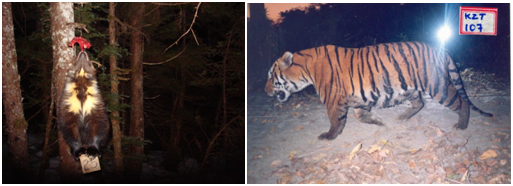
\includegraphics[width=5in]{Ch1/figs/wolverinetiger.png}
\end{center}
\caption{
Left: Wolverine being encounter by a
camera trap ({\it Photo credit: Audrey Magoun}).
Right: Tiger encountered by
camera trap ({\it Photo credit: Ullas Karanth}).
}
\label{fig.wolverinetiger}
\end{figure}

In camera trapping studies, cameras are often situated along trails or at
baited stations and individual animals are photographed and
subsequently identified either manually by a person sitting behind a
computer, or sometimes now using specific identification
software. Camera trapping methods are widely used for species that
have unique stripe or spot patterns such as tigers
\citep{karanth:1995, karanth_nichols:1998}, ocelots ({\it Leopardus
  pardalis }; \citep{trolle_kery:2003,trolle_kery:2005}), leopards
({\it Panthera pardus}; \citep{balme_etal:2010}), and many other cat
species.  Camera traps are also used for other species such as
wolverines ({\it Gulo gulo};
\citep{magoun_etal:2011,royle_etal:2011jwm}), and even species that
are less easy to identify uniquely such as mountain lions ({\it Puma
  concolor}, \citep{sollmann_etal:inprepjapplecol}) and coyotes ({\it
  Canis latrans}, \citep{kelly_etal:2008}).  We note that even for
species that are not readily identified by pelage patterns, it might
be efficient to use camera traps in conjunction with spatial
capture-recapture models to estimate density (see
Chapts.~\ref{chapt.scr-unmarked} and \ref{chapt.partialID}).
%, if an initial sample of individuals can be collared
%or tagged in some way so that subsequent encounter by camera-traps can
%yield individual information. In this way, the probability of
%encounter can be estimated from the camera traps based on the
%pre-marked individuals, and this is applied to the frequencies of
%unmarked individuals to estimate density.







\subsection{DNA sampling}

DNA obtained from hair, blood or scat is now routinely used to obtain
individual identity and encounter history information about
individuals \citep{taberlet_bouvent:1992, kohn_etal:1999,
  woods_etal:1999, mills_etal:2000, schwartz_monfort:2008}.  A common
method is based on the use of ``hair snares'' (Fig. \ref{fig.bearcat})
which are widely used to study bear populations
\citep{woods_etal:1999, garshelis_etal:2006,
  kendall_etal:2009,gardner_etal:2010jwm}.  A sample of hair is obtained as individuals
pass under or around barbed-wire (or other physical mechanism) to take
bait. Hair snares and scent sticks have also been used to sample felid
populations \citep{garciaalaniz_etal:2010, kery_etal:2010} and other
species. Research has even shown that DNA information can be extracted
from urine deposited in the wild (e.g., in snow; see
\cite{valiere_taberlet:2000}) and as a result this may prove another
future data collection technique where SCR models are useful.

\begin{figure}
\begin{center}
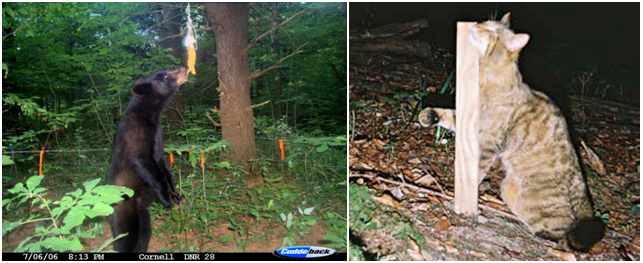
\includegraphics[width=5in]{Ch1/figs/bearcat}
\end{center}
\caption{Left:  Black bear in a hair snare ({\it Photo credit: M. Wegan})
Right: European wildcat loving on a scent stick ({\it Photo credit: Darius
Weber
%, Hintermann \& Weber AG, Ecological Consultancy, Planning \&
%Research, Switzerland
})
}
\label{fig.bearcat}
\end{figure}


\begin{figure}
\begin{center}
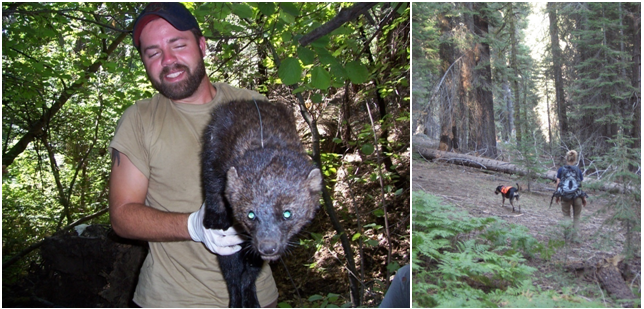
\includegraphics[width=5in]{Ch1/figs/beardog}
\end{center}
\caption{Left:
A wildlife research technician for the USDA Forest Service
  holding a male fisher  captured as part of the Kings River Fisher
  Project in the Sierra National Forest, California.
Right: A dog handler surveying for fisher scat in the Sierra National Forest.
{\it Photo credit: Craig Thompson}.}
%, USDA Forest Service,
%Pacific Southwest Research Station.}}
\label{fig.fisherscatdog}
\end{figure}


\subsection{Acoustic sampling}

Many studies of birds \citep{dawson_efford:2009}, bats, and whales
\citep{marques_etal:2009} now collect data using devices that record
vocalizations. When vocalizations can be identified by individual from
multiple recording devices, spatial encounter histories are produced
that are amenable to the application of SCR models
\citep{dawson_efford:2009, efford_etal:2009ecol}. Recently, these
ideas have been applied to data on direction  or distance to
vocalizations by multiple simultaneous observers and related problems
(D. Borchers, ISEC 2012 presentation).


\subsection{Search-encounter methods}

There are other methods which don't fall into a nice clean taxonomy of
``devices''. Spatial encounter histories are commonly obtained by
conducting manual searches of geographic sample units such as
quadrats, transects or road or trail networks.  For example, DNA-based
encounter histories can be obtained from scat samples located along
roads or trails or by specially trained dogs \citep{mackay_etal:2008}
searching space (Fig. \ref{fig.fisherscatdog}). This method has been
used in studies of martens, fishers \citep{thompson_etal:2012},
lynx, coyotes, birds \citep{kery_etal:2010}, and many other species.
A similar data structure arises from the use of standard territory or
spot mapping of birds \cite{bibby_etal:1992} or area sampling in which
space is searched by observers to physically capture individuals.
This is common in surveys that involve reptiles and amphibians, e.g.,
we might walk transects picking up box turtles \citep{hall_etal:1999},
or desert tortoises \citep{zylstra_etal:2010}, or search space for
lizards \citep{royle_young:2008}.

These methods don't seem like normal capture-recapture in the sense
that the encounter of individuals is not associated with specific trap
location, but SCR models are equally relevant for analysis of such
data as we discuss in Chapt. \ref{chapt.search-encounter}.




\section{Capture-Recapture for Modeling Encounter Probability}

We briefly introduced techniques used for the study of animal
populations. These methods produce individual encounter history data,
a record of where and when each individual was captured. We refer to
this as a {\it spatial encounter history}. Historically, auxiliary
spatial information has been ignored, and encounter history data have
been {\it summarized} to simple ``encounter or not'' for the purpose
of applying ordinary CR models.  The basic problem with these ordinary
(or ``non-spatial'') capture-recapture models is they don't have any
sense of space in them, the spatial information is summarized out of
the data set, so we aren't able to use such models for studying things
such as movement, or resource selection, etc..  Instead, ordinary
capture-recapture models usually resort to models of ``encounter
probability,'' which is a nuisance parameter, seldom of any ecological
relevance.  We show an example here that is in keeping with the
classical application of ordinary capture-recapture models.

%In terms of density estimation,  there is no
%linkage {\it in the model} between the quantity being informed by the
%data (i.e., $N$) and any stated or prescribed ``area'', $A$.



\subsection{Example: Fort Drum bear study}

Here we confront the simplest possible capture-recapture problem,
estimating density from a standard capture-recapture study, but one of
applied interest. We use this as a way to introduce some concepts
and motivate the need for spatial capture-recapture models by
confronting technical and conceptual problems that we encounter. The
data come from a study to estimate black bear abundance on the Fort
Drum Military Installation in upstate New York ( \citet{wegan:2008}, see
also Chapt. \ref{chapt.closed} for more details). The specific data used
here are encounter histories on 47 individuals obtained from an array
of 38 baited ``hair snares'' during June and July 2006. The study area
and locations of the 38 hair snares are shown in
Fig. \ref{fig.hairsnares}.  Barbed wire traps (see
Fig. \ref{fig.bearcat}) were baited and checked for hair samples each
week for eight weeks.  Analysis of these data appears in \citet{gardner_etal:2009} and
\citet{gardner_etal:2010jwm}, and we use the data in a number of
analyses in later chapters.

\begin{figure}[ht]
\begin{center}
\includegraphics[height=3in]{Ch1/figs/hairsnares}
\end{center}
\caption{Locations of hair snares on Fort Drum, New York, operated
  during the summer of 2006 to sample black bears.}
\label{fig.hairsnares}
\end{figure}

Although each bear was captured, or not, in each of the 38 hair
snares, we start by treating this data set as a standard capture-recapture data
set and summarize to an encounter history matrix with 47 rows and 8
columns with entries $y_{ik}$, where $y_{ik}=1$ if individual $i$ was
captured, at any trap, in sample occasion $k$ and $y_{ik}=0$
otherwise. There is a standard closed population model, colloquially
referred to as ``model $M_0$'' (see Chapt. \ref{chapt.closed}), which
assumes that encounter probability $p$ is constant for all individuals
and sample periods.  We fitted model $M_0$ to the Fort Drum data using
traditional likelihood methods, yielding the maximum likelihood
estimate (MLE) of $\hat{N} = 49.19$ with an asymptotic standard error
(SE) of $1.9$.

The key issue in using such a closed population model regards how we
should interpret this estimate of $N=49.19$ bears. Does it represent
the entire population of Fort Drum? Certainly not -- the trapping
array covers less than half of Fort Drum as we see in
Fig. \ref{fig.hairsnares}. So to get at the total bear population size
of Fort Drum, we would have to convert our $\hat{N}$ to an estimate of
density and extrapolate. To get at density, then, should we assert
that $N$ applies to the southern half of Fort Drum below some
arbitrary line? Surely bears move on and off of Fort Drum without
regard to hypothetical boundaries. Without additional information
there is simply no way of converting this estimate of $N$ to density,
and hence it is really not meaningful biologically. To resolve this
problem, we will adopt the customary approach of converting $N$ to $D$
by buffering the convex hull around the trap array. The convex hull
has area $157.135$ $km^2$. We follow \citet{bales_etal:2005} in
buffering the convex hull of the trap array by the radius of the mean
female home range size.


%%%%\footnote{Did Bales et al. actually do this?}.
%HERE IS WHAT BALES DID:  First, we created a 95% minimum convex polygon
%for all radiolocations of adult females used in homerange
%analyses (Figure 1). Second,we buffered the
%100% minimum convex polygon for trapping locations
%with the approximate radius of the average
%95% minimum convex polygon home range of adult
%females (n = 13) using ArcView (ESRI, Redlands,
%Calif.).

The mean female home range radius was estimated \citep{wegan:2008} for
this study region to be $2.19$ km,
%\footnote{Is this number right out of Wegan's disseration?}
% YES, this is straight out of his thesis.
and the area of the convex hull buffered by $2.19$ km is $277.01$
km$^2$. ({\bf R} commands to compute the convex hull, buffer it, and
compute the area are given in the {\bf R} package \mbox{\tt scrbook}
which accompanies the book).  Hence, the estimated density here is
approximately $0.178$ bears/km$^2$ using the estimated population size
obtained by model $M_0$.  We could assert that the problem has been
solved, go home, and have a beer.  But then, on the other hand, maybe
we should question the use of the estimated home range radius -- after
all, this is only the female home range radius and the home ranges
change for many reasons. Instead, we may decide to rely on a buffer
width based on one-half mean maximum distance moved (MMDM) estimated
from the actual hair snare data as is more customary
\citep{dice:1938}. In that case the buffer width is $1.19$ km, and the
resulting estimated density is increased to $0.225$ bears/km$^2$ about
27 \% larger.  But wait -- some studies actually found the full MMDM
\citep{parmenter_etal:2003} to be a more appropriate measure of
movement (e.g \citet{soisalo_cavalcanti:2006}). So maybe we should use
the full MMDM which is $2.37$ km, pretty close to the telemetry-based
estimate and therefore providing a similar estimate of density
($0.171$ bears/km$^2$). So in trying to decide how to buffer our trap
array we have already generated 3 density estimates. The crux of the
matter is obvious: Although it is intuitive that $N$ should scale with
area -- the number of bears should go up as area increases and go down
as area decreases -- in this ad hoc approach of accounting for animal
movement $N$ remains the same, no matter what area we assert was
sampled. The number of bears and the area they live in are not
formally tied together within the model, because estimating $N$ and
estimating the area $N$ relates to are two completely independent
analytical steps which are unrelated to one another by a formal model.

Unfortunately, our problems don't end here. In thinking about the use
of model $M_0$, we might naturally question some of the basic
assumptions that go into that model. The obvious one to question is
that which declares that $p$ is constant. One obvious source of
variation in $p$ is variation {\it among individuals}. We expect that
individuals may have more or less exposure to trapping due to their
location relative to traps, and so we try to model this
``heterogeneous'' encounter probability phenomenon.
To illustrate
this phenomenon,  here are the
number of traps that each individual
was encountered in:
\begin{verbatim}
 # traps:  1   2  3  4  5  6  9
 # bears: 23  13  6  2  1  1  1
\end{verbatim}
meaning, for example, 23 bears were captured in only 1 trap, and 1
bear was captured in 9 distinct traps. The variation in trap-encounter
frequencies suggests quite a range in traps exposed to bears in the
sampled population.
%%% #bears: 19 15  5  2  2  1  1  1  1
% But, being captured in different numbers of traps is {\it not}
% inconsistent with a non-spatial model.  That is if individuals
% roamed randomly over space with no ``home range'' then you should
% expect them to be captured in varying numbers of traps also.....
Historically, researches try to reduce spatial heterogeneity in
capture probability by placing $>1$ trap per home range
\citep{otis_etal:1978, williams_etal:2002}. This seems like a sensible
idea but it is difficult to do in practice since you don't know where
all the home ranges are and so we try to impose a density of traps
that averages something $>1$ per home range.  An alternative solution
is to fit models that allow for individual heterogeneity in $p$
\citep{karanth:1995}. Such models have the colloquial name of ``model
$M_h$'' \citep{otis_etal:1978}.  We fitted this model (see
Chapt. \ref{chapt.closed} for details) to the Fort Drum data using
each of the 3 buffer widths previously described (telemetry, 1/2 MMDM
and MMDM), producing the estimates reported in Table
\ref{intro.tab.fdests}. While we can tell by the models' AIC that
$M_h$ is clearly favored by more than 30 units, we might still not be
entirely happy with our results. Clearly there is information in our
data that could tell us something about the exposure of individual
bears to the trap array -- where they were captured, and how many
times -- but since space has no representation in our model, we can't
make use of this information. Model $M_h$ thus merely accounts for
what we observe in our data (some bears were more frequently captured
than others) rather than explicitly accounting for the processes that
generated the data.

So what are we left with?  Our density estimates span a range from
$0.17$ to $0.43$ bears/km$^2$ depending on which estimator of $N$ we
use and what buffer strip we apply. Should we feel strongly about one
or the other?  Which buffer should we prefer?  AIC favors model $M_h$,
but did it adequately account for the differences in exposure of
individuals to the trap array? Are we happy with a purely
phenomenological model for heterogeneity?  It assumes that all
individuals are independent and identically distributed ($iid$) draws
from some distribution, but does not account for the explicit
mechanism of induced heterogeneity. And, further, we have information
about that (trap of capture) which model $M_h$ ignores.
% Moreover, we could find more variations of model Mh to choose among,
% but see \citep{link:2003}.
And if we choose one type of buffer, how do we compare our density
estimates to those from other studies that may opt for a different
kind of buffer?  The fact that $N$ does not scale with $A$, as part of
the model, renders this choice arbitrary.



\begin{table}[ht]
\centering
\caption{Table on estimates of density ($D$, bears/$km^2$) for the Fort Drum data
using models $M_0$ and $M_h$ and different buffers. Model $M_h$ here
is a logit-normal mixture \citep{coull_agresti:1999}.}
\begin{tabular}{ll|cc}
\hline \hline
Model & Buffer &  $\hat{D}$ & SE \\ \hline
$M_0$   & telemetry &  0.178 & 0.178 \\
$M_0$    & MMDM     &  0.171 & 0.171\\
$M_0$   & 1/2 MMDM  &  0.225 & 0.225\\
$M_h$ & telemetry &0.341 & 0.144\\
$M_h$ & MMDM    &  0.327 & 0.138\\
$M_h$ & 1/2 MMDM & 0.432 & 0.183\\ \hline
\end{tabular}
\label{intro.tab.fdests}
\end{table}


\subsection{Inadequacy of non-spatial capture-recapture}

The parameter $N$ (population size) in an ordinary capture-recapture
model is functionally unrelated to any notion of sample area, and so
we are left taking arbitrary guesses at area, and matching it up with
estimates of $N$ from different models that do not have any explicit
biological relevance.  Clearly, there is not a compelling solution to
be derived from this ``estimate $N$ and conjure up a buffer'' approach
and we are left not much wiser about bear density at Fort Drum than we
were before we conducted this analysis, and certainly not confident in
our assessments.  Closed population models are not integrated with any
ecological theory, so our $N$ is not connected to the specific
landscape in any explicit way.

The capture-recapture models that we used apply to truly closed
populations -- a population of goldfish in a fish bowl. Yet here we
are applying them to a population of bears that inhabit a rich
two-dimensional landscape of varied habitats, exposed to trapping by
an irregular and sparse array of traps. It seems questionable that the
same model that is completely sensible for a population of goldfish in
a bowl, should also be the right model for this population of bears
distributed over a broad landscape.  Ordinary capture-recapture
methods are distinctly non-spatial. They don't admit spatial indexing
of either sampling (the observation process) or of individuals (the
ecological process). This leads immediately to a number of practical
deficiencies: (1) Ordinary CR models do not provide a coherent basis
for estimating density, a problem we struggled with in the black bear
study.  (2) Ordinary CR model and sampling methods {\it induce} a form
of heterogeneity that can only at best be approximated by classical
models of latent heterogeneity. SCR models formally accommodate
heterogeneity due to the juxtaposition of individuals with the
encounter devices.  (3) Ordinary CR models do not accommodate
trap-level covariates which exist in a large proportion of real
studies; (4) Ordinary CR models do not accommodate formal
consideration of any spatial process that gives rise to the observed
data.

In subsequent chapters of this book, we resolve these specific
technical problems related to density, model-based linkage of N and A,
covariates, spatial variation, and related things all within a
coherent unified framework for spatial capture-recapture.


\section{ Historical Context: A Brief Synopsis}

Spatial capture-recapture is a relatively new methodological
development, at least with regard to formal estimation and
inference. However, the basic problems that motivate the need for
formal spatially-explicit models have been recognized for decades and
quite a large number of ideas have been proposed to deal with these
problems. We review some of these ideas here.

\subsection{Buffering}

The standard approach to estimating density even now is to estimate
$N$ using conventional closed population models \citep{otis_etal:1978}
and then try to associate with this estimate some specific sampled
area, say $A$, the area which is contributing individuals to the
population for which $N$ is being estimated. The strategy is to define
$A$ by placing a buffer of say $W$ around the trap array or some
polygon which encloses the trap array. The historical context is
succinctly stated by \citep{obrien:2011} from which we draw this
description:

\begin{quote}
  ``At its most simplistic, $A$ may be described by a concave polygon
  defined by connecting the outermost trap locations ($A_{tp}$;
  \citet{mohr:1947}).  This assumes that animals do not move from
  outside the bounded area to inside the area or vice versa. Unless
  the study is conducted on a small island or a physical barrier is
  erected in the study area to limit movement of animals, this
  assumption is unlikely to be true. More often, a boundary area of
  width $W$ ($A_{w}$) is added to the area defined by the polygon
  $A_{tp}$ to reflect the area beyond the limit of the traps that
  potentially is contributing animals to the abundance estimate
  \citep{otis_etal:1978}. The sampled area, also known as the
  effective area, is then $A(W) = A_{tp} + A_{w}$. Calculation of the
  buffer strip width ($W$) is critical to the estimation of density
  and is problematic because there is no agreed upon method of
  estimating $W$. Solutions to this problem all involve ad hoc methods
  that date back to early attempts to estimate abundance and home
  ranges based on trapping grids
  \citep[see][]{hayne:1949}. \citet{dice:1938} first drew attention to
  this problem in small mammal studies and recommended using one-half
  the diameter of an average home range. Other solutions have included
  use of inter-trap distances \citep{blair:1940, burt:1943}, mean
  movements among traps, maximum movements among traps
  \citep{holdenried:1940, hayne:1949}, nested grids
  \citep{otis_etal:1978}, and assessment lines
  \citep{smith_etal:1971}.''
\end{quote}

The idea of using 1/2 mean maximum distance moved
\citep[``MMDM''][]{wilson_anderson:1985a} to create a buffer strip
seems to be the standard approach even today, presumably justified by
Dice's suggestion to use 1/2 the home range diameter, with the mean
over individuals of the maximum distance moved being an estimator of
home range diameter. Alternatively, some studies have used the full
MMDM (e.g. \citet{parmenter_etal:2003}), because the trap array might
not provide a full coverage of the home range (home ranges near the
edge should be truncated) and so 1/2 MMDM should be biased smaller
than the home range radius.  And, sometimes home range size is
estimated by telemetry \citep{karanth:1995, bales_etal:2005}.
% \footnote{Is this correct cite for this?}.  Karanth used some
% technique, it's hard to tell for sure....but he mentions using 1
% female that is collared to estimate effective trap area.  Bales does
% it too, so I added it for extra value!
Use of MMDM summaries to estimate home range radius is usually
combined with an AIC-based selection from among the closed-population
models in \citet{otis_etal:1978} which most often suggests
heterogeneity in detection (model $M_h$).  Almost all of these early
methods were motivated by studies of small mammals using classical
``trapping grids'' but, more recently, their popularity in the study
of wildlife populations has increased with the advent of new
technologies, especially related to non-invasive sampling methods such
as camera trapping. In particular, the series of papers by Karanth and
Nichols \citep{karanth:1995, karanth_nichols:1998,
  karanth_nichols:2002} has led to fairly widespread adoption of these
ideas.

\begin{comment}
Some of the heuristic ideas based on buffer strips do have some
technical justification in the sense of estimating parameters of an
underlying movement model from observed movements. For example, if we
let $x$ be a random variable indicating movement outcomes of an
individual about its  home range center, and suppose that $x$ has pdf
$g(x)$ then we can understand properties of MMDM by studying the
properties of the sample order statistics, as the maximum distance
moved is the sample range based on a sample of observations of
individual locations.
\end{comment}


%As an illustration, imagine a 1-dimensional
%system where individuals have a home range that amounts to a line
%segment. Then suppose that individual movements are $\mbox{uniform}(0,A)$. It
%can be shown that the sampling distribution of the sample range, R,
%scaled by $A$, say $R/A$ has a beta distribution, $\mbox{beta}(n-1,2)$
%\citep[][p. 235]{casella_berger:2002}
%and thus the diameter of the home range, i.e. $A$, is
%estimated (biasedly) by$ R/( (n-1)/(n+1) )$. For large $n$ we could then
%say that the sample range, i.e., ''maximum distance moved'' seems like a good estimator of home range diameter and, therefore, $R/2$ is an estimator of home-range radius.

%There are a number of technical issues that arise in attempting to use
%such heuristics to justify the application in practice. For one, the
%moments of the sample order statistics are strongly affected by sample
%size, which is typically quite small (per individual encountered) and
%thus, in general, are biased and estimated with variable precision
%depending on sample size. For example, the expected value of MMDM is
%$k(n)*A$ , i.e., the true home range diameter is related to observed
%MMDM by some function of sample size, $k(n)$, that increases to 1. In
%the case where the underlying movement model is uniform, $k(n) =
%(n-1)/(n+1)$ (from above) which motivates a formula for ``adjusting''
%observed MMDM for small sample size. We suspect that many such
%formulae are obtainable depending on the assumed movement distribution
%\citep[e.g., formula 6.16 in][]{obrien:2011}. We might also think about taking
%the {\it maximum} (over individuals) of the maximum distance moved
%because under the specific model considered here (iid uniform) then
%all individuals have the same home range radius. This increases our
%sample size ($n$) and thus the observed sample range should be more
%accurate.


%%Another issue of somewhat more importance (and less easy to
%rectify) is that the {\it observation} of movement outcomes is biased
%by the locations of traps. We cannot observe movements ``off the
%trapping grid'' (or between traps) and thus our observed movements
%will generally be smaller than expected under any particular model
%(the uniform in this case). Moreover, the trap spacing also induces a
%discreteness to the movements that causes a further level of
%approximation based on hypothetical movement
%distributions. Nevertheless, formal analysis of `` buffering''
%strategies based on sample order statistics under specific models for
%movement does at least provide some heuristic support for specific
%choices.  The interested reader should ponder the distribution of the
%sample minimum, maximum and range under other distributions such as a
%normal (and bivariate normal), exponential distribution and perhaps
%others. In addition, contemplate the effect of censoring of movements
%to some arbitrary limit ($B<A$) to mimic bias in observed movement
%outcomes due to a finite trap grid.
\begin{comment}
\subsection{Trapping webs}

The use of buffer strips is conventional and widespread due to the
heuristic appeal of that idea and its easy implementation, but other
conceptual approaches exist to address specific problems motivated by
the spatial context of capture-recapture data. D.R. Anderson came up
with the idea of the ``trapping web'' \citep{anderson_etal:1983} which
does not seem to have been widely adopted in practice.
% although there
%is a clear mathematical formalization to the trapping web design
%\citep{link_barker:1994}.
One reason for this is the design is somewhat restrictive in the sense
that it requires a large number of traps be organized in close
proximity to one another.
\end{comment}

\subsection{Temporary emigration}

Another intuitively appealing idea is that by \citet{white_shenk:2000}
who discuss ``correcting bias of grid trapping estimates'' by
recognizing that the basic problem is like random temporary emigration
\citep{kendall_etal:1997,
  chandler_etal:2011,ivan_etal:2013a,ivan_etal:2013b} where
individuals flip a coin with probability $\phi$ to determine if they
are ``available'' to be sampled or not.  White and Shenk's idea was to
estimate $\phi$ from radio telemetry, as the proportion of time an
individual spends in the study area. They obtain the estimated
``super-population'' size by using standard closed population models
and then obtain density by $\hat{D} = \hat{N}\hat{\phi}/A$ where $A$
is the nominal area of the trapping array (e.g., minimum convex hull).
A problem with this approach is that individuals that were radio
collared represent a biased sample i.e., you fundamentally have to
sample individuals randomly from the population {\it in proportion to
  their exposure to sampling} and that seems practically impossible to
accomplish. In other words, ``in the study area'' has no precise
meaning itself and is impossible to characterize in almost all
capture-recapture studies.  Deciding what is ``in the study area'' is
effectively the same as choosing an arbitrary buffer which defines who
is in the study area and who isn't.  That said, the temporary
emigration analogy is a good heuristic for understanding SCR models
and has a precise technical relevance to certain models.

Another interesting idea is that of using some summary of ``average
location'' as an individual covariate in standard capture-recapture
models. \citet{boulanger_mclellan:2001} use distance-to-edge (DTE) as
a covariate in the Huggins-Alho type of model. \citet{ivan:2012} uses
this approach in conjunction with an adjustment to the estimated $N$
obtained by estimating the proportion of time individuals are ``on the
area formally covered by the grid'' using radio telemetry.  We do not
dwell too much on these different variations but we do note that the
use of DTE as an individual covariate amounts to some kind of
intermediate model between simple closed population models and fully
spatial capture-recapture models, which we address directly in
Chapt. \ref{chapt.closed}.
%We note that no adjustment
%based on telemetry information is necessary if one were simply to
%place a prior distribution on the individual covariate (which is not
%to say that telemetry data isn't useful, just that the same objective
%can be achieved without telemetry data).

While these procedures are all heuristically appealing, they are also
essentially ad hoc in the sense that the underlying model remains
unspecified or at least imprecisely characterized and so there is
little or no basis for modifying, extending or generalizing the
methods. These methods are distinctly {\it not} model-based
procedures.  Despite this, there seems to be an enormous amount of
literature developing, evaluating and ``validating'' these literally
dozens of heuristic ideas that solve specific problems, as well as
various related tweeks and tunings of them and really it hasn't led to
any substantive breakthroughs that are sufficiently general or
theoretically rigorous.



%A classical argument in favor of the HA model is
%that it ``doesn't require assumptions about the covariate'' but the
%assumption is explicit in capture-recapture models and thus it is
%natural to attack inference based on the ``joint likelihood''
%\citep{borchers_etal:2002}. This has proven necessary in certain other
%classes of individual covariate models in which natural models arise
%for the individual covariate, such as time-varying individual
%covariates \citep{bonner_schwarz:2006}, or covariates with measurement
%error (e.g., distance sampling; see
%\citet[][ch. 7]{royle_dorazio:2008}).
%The model-based formulation is easily adapted to standard
%individual covariate models as well \citep{royle:2008}. Throughout
%this book we rely heavily on Bayesian inference of the joint
%likelihood, using the formulation based on data-augmentation
%\citep{royle_etal:2007, royle_young:2008, royle:2009} though we also
%discuss the development of likelihood-based inference in chapter 5 and
%apply those methods in some cases.






\section{Extension of Closed Population Models}



The deficiency with classical closed population models is that they
have no spatial context. $N$ is just an integer parameter that applies
equally well to estimating the number of unique words in a book, the
size of some population that exists in a computer, or a bucket full of
goldfish.  The question of {\it where} the $N$ items belong is central
both to interpretation of data and estimates from all
capture-recapture studies and, in fact, to the construction of spatial
capture-recapture models considered in this book.  Surely it must
matter whether the $N$ items exist as words in a book, or goldfish in
a bowl, or tigers in a patch of forest! That classical closed
population models have no spatial context leads to a number of
conceptual and methodological problems or limitations as we have
encountered previously. More important, ecologists seldom care only
about $N$ -- space is often central to objectives of many population
studies -- movement, space usage, resource selection, how individuals
are distributed in space and in response to explicit factors related
to landuse or habitat. Because space is central to so many real
problems, this is probably the number 1 reason that many ecologists
don't bother with capture-recapture. They haven't seen
capture-recapture methods as being able to solve their problems.

Thus, the essential problem is that classical closed population models
are too simple - they ignore the spatial attribution of traps and
encounter events, movement and variability in exposure of individuals
to trap proximity, and, because ordinary closed population models
possess no notion of ``area'', they do not yield estimates of {\it
  density}, a model of movement or space-usage, or how density varies
over space. These problems can be addressed formally by the
development of more general models.



\subsection{Towards spatial explicitness: Efford's formulation}

%Spatial capture-recapture models are
%statistical and mathematical models that extend non-spatial
%``ordinary'' capture-recapture models to accommodate the spatial
%structure inherent in sampling animal populations - i.e., trap
%locations, individual locations, and individual use of space.

The solution to the various issues that arise in the application of
ordinary capture-recapture models is to extend the closed population
model so that $N$ becomes spatially explicit.
%A natural way is to
%define a point process \citep{efford:2004} that describes how
%individuals are organized in space and that, when points are
%aggregated over space, the value $N$ is derived in a meaningful way.
%Thus, in this book, we adopt the view that the locations of the $N$
%individuals in the population are a {\it realization of a spatial
%  point process}.
\citet{efford:2004} was the first to formalize an explicit model for
spatial capture-recapture problems in the context of trapping arrays.
He adopted a Poisson point process model to describe the distribution
of individuals and essentially a distance sampling formulation of the
observation model which describes the probability of detection as a
function of individual location, regarded as a latent variable
governed by the point process model. While earlier (and contemporary)
methods of estimating density from trap arrays have been ad hoc in the
sense of lacking a formal description of the spatial model, Efford
achieved a formalization of the model, describing explicit mechanisms
governing the spatial distribution of individuals and how they are
encountered by traps, but adopted a more or less ad hoc framework for
inference under that spatial model using a simulation based method
known as inverse prediction \citep{gopalaswamy:2012}.

Recently, there has been a flurry of effort devoted to formalizing
inference under this model-based framework for the analysis of spatial
capture-recapture data
\citep{royle_gardner:2011,borchers:2011,gopalaswamy:2012}.  There are
two distinct lines of work which adopt the model-based formulation in
terms of the underlying point process but differ primarily by the
manner in which inference is achieved. One approach
\citep{borchers_efford:2008} uses classical inference based on
likelihood (see Chapt. \ref{chapt.mle}), and the other
\citep{royle_young:2008} adopts a Bayesian framework for inference
(Chapts. \ref{chapt.scr0} and \ref{chapt.mcmc}).

\begin{comment}
To motivate the origins and relevance of these approaches, we note
that, fundamentally, spatial capture-recapture models are related to
classical ``individual covariate'' models (colloquially referred to as
Huggins-Alho models) in capture-recapture \citep{huggins:1989,
  alho:1990}.  In particular, the individual covariate\footnote{have
  we mentioned what the individual covariate is, yet?} is observed in
these classical individual covariate models whereas it is not directly
observed in SCR models.  To accommodate that, a prior distribution for
the individual covariate is required.
%In essence then, SCR models are
%similar to a fully model-based formulation of classical Huggins-Alho
%models (see \citet{royle:2009}).
Likelihood analysis
\citep{borchers_efford:2008} proceeds by removing the random effect
from the likelihood by integration whereas Bayesian analysis
\citep{royle_young:2008} proceeds by analyzing the conditional model
directly, usually by methods of Markov chain Monte Carlo (MCMC).
\end{comment}



\subsection{Abundance as the aggregation of a point process}

Spatial point process models represent a major methodological theme in
spatial statistics \citep{cressie:1992} and they are widely applied as
models for many ecological phenomena
\citep{stoyan_penttinen:2000,illian_etal:2008}. Point process models
apply to situations in which the random variable in question
represents the locations of events or objects: trees in a forest,
weeds in a field, bird nests, etc.  As such, it seems natural to
describe the organization of individuals in space using point process
models. SCR models represent the extension of ordinary
capture-recapture by augmenting the model with a point process to
describe individual locations.

Specifically, let ${\bf s}_{i}; i=1,2,\ldots,N$ be the locations of
all individuals in the population.  One of the key features of SCR
models is that the point locations are latent, or unobserved, and we
only obtain imperfect information about the point locations by
observing individuals at trap or observation locations.  Thus, the
realized locations of individuals represent a type of ``thinned''
point process, where the thinning mechanism is not random but, rather,
biased by the observation mechanism.  It is also natural to think
about the observed point process as some kind of a compound or
aggregate point process with a set of ``parent'' nodes being the
locations of individual home ranges or their centroids, and the
observed locations as ``offspring'' - i.e., a Poisson cluster process
(PCP). In that context, density estimation in SCR models is analogous
to estimating the number of parents of a Poisson cluster process
\citep{chandler_royle:2012}.
% Other types of point
% process models for the realized locations have direct relevance to SCR
% models (See \citet{chandler_royle:2012}, discussed in chapter XYZ).

Most of the recent developments in modeling and inference from spatial
encounter history data, including most methods discussed in this book,
are predicated on the view that individuals are organized in space
according to a relatively simple point process model. More
specifically, we assume that the collection of individual activity
centers are independent and identically distributed random variables
distributed uniformly over some region. This is consistent with the
assumption that the activity centers represent the realization of a
Poisson point process or, if the total number of activity centers if
fixed, then this is usually referred to as a binomial point process.


\subsection{The activity center concept}

In the context of SCR models, and because most animals we study by
capture-recapture are not sessile, there is not a unique and precise
mathematical definition of the point locations ${\bf s}$.  Rather, we
imagine these to be the centroid of individuals home ranges, or the
centroid of an individual's activities during the time of sampling, or
even it's average location measured with error (e.g., from a long
series of telemetry measurements). In general, this point is unknown
for any individual but if we could track an individual over time and
take many observations then we could perhaps get a good idea of where
that point is.  We'll think of the collection of these points as
defining the spatial distribution of individuals in the population.

%%I think we could shorten the home range paragraph; I like the definition
%%'the centroid of an individual's
%%% activities during the time of sampling'. I think the definition of
%% home range is something like the colleciton of points/sites/areas
%% an animal uses over the course of its lifetime so it's vague anyway
%% and what that definition means for the different forms of home
%%ranges - territory, migratory species etc - is pretty much left open.

We use the terms home range or activity center interchangeably. The
term ``home range center'' suggests that models are only relevant to
animals that exhibit behavior of establishing home ranges or
territories, or central place foragers, and since not all species do
that, perhaps the construction of SCR models based on this idea is
flawed. However, the notion of a home range center is just a
conceptual device and we don't view this concept as being strictly
consistent with classical notions of animal territories. Rather our
view is that a home range or territory is inherently dynamic,
temporally, and thus it is a transient quantity - where the animal
lived during the period of study, a concept that is completely
analogous to the more conventional notion of utilization
distributions.  Therefore, whether or not individuals of a species
establish home ranges is irrelevant because, once a precise time
period is defined, this defines a distinct region of space that an
individual must have occupied.



\subsection{The state-space}

Once we introduce the collection of activity centers, ${\bf s}_{i};
i=1,2,\ldots,N$, then the question ``what are the possible values of
${\bf s}$?'' needs to be addressed because the individual ${\bf
  s}_{i}$ are {\it unknown}. As a technical matter, we will regard
them as random effects and in order to apply standard methods of
statistical inference we need to provide a distribution for these
random effects.  In the context of the point process model, the
possible values of the point locations referred to as the
``state-space'' of the point process and this is some region or set of
points which we will denote by ${\cal S}$. This is analogous to what
is sometimes called the {\it observation window} for ${\bf s}$ in the
point process literature.  The region ${\cal S}$ serves as a prior
distribution for ${\bf s}_{i}$ (or, equivalently, the random effects
distribution).
%%Don't think prior has come up yet; maybe not that important here?
In animal studies, as a description of where individuals that could be
captured are located, it includes our study area, and should
accommodate all individuals that could have been captured in the study
area.  In the practical application of SCR models, in most cases
estimates of density will be relatively insensitive to choice of
state-space which we discuss further in Chapt. \ref{chapt.scr0} and
elsewhere.


\subsection{Abundance and density}

When the underlying point process is well-defined, including a precise
definition of the state-space, this in turn induces a precise
definition of the parameter $N$, ``population size'', as the number of
individual activity centers located within the prescribed state-space,
and its direct linkage to density, $D$. That is, if $A({\cal S})$ is
the area of the state-space then
\[
 D = \frac{N}{ A({\cal S})}.
\]
A deficiency with some classical methods of ``adjustment'' is they
attempted to prescribe something like a state-space - a ``sampled
area'' - except absent any precise linkage of individuals with the
state-space. SCR models formalize the linkage between individuals and
space and, in doing so, provide an explicit definition of $N$
associated with a well-defined spatial region, and hence density. That
is, the provide a model in which $N$ scales, as part of the model,
with the size of the prescribed state-space. In a sense, the whole
idea of SCR models is that by defining a point process and its
state-space ${\cal S}$, this gives context and meaning to $N$ which
can be estimated directly for that specific state-space. Thus, it is
fixing ${\cal S}$ that resolves the problem of ``unknown area'' that
we have previously discussed.



\section{Characterization of SCR models}

Formulation of capture-recapture models conditional on the latent
point process is the critical and unifying element of {\it all} SCR
models.

SCR models differ in how the underlying process model is formulated,
or its complexity.  Most of the development and application of SCR
models has focused on their use to estimate density and touting the
fact that they resolve certain specific technical problems related to
the use of ordinary capture-recapture models. This is achieved with a
simple process model being a basic point process of independently
distributed points.  At the same time, there are models of CR data
that focus exclusively on {\it movement} modeling, or models with
explicit dynamics \citep{ovaskainen:2004,
  ovaskainen_etal:2008}. Conceptually, these are akin to spatial
versions of so-called Cormack-Jolly-Seber (CJS) models in the
traditional capture-recapture literature, except they involve explicit
mathematical models of movement based on diffusion or Brownian motion.
Finally, there are now a very small number of papers that focus on
{\it both} movement and density simultaneously
\citep{royle_young:2008, royle_etal:2011mee, royle_chandler:2012} or
population dynamics and density \citep{gardner_etal:2010jwm}.

A key thing is that these models, whether focused just on density, or
just on movement, or both, are similar models in terms of the
underlying concepts, the latent
structure, and the observation model. They are rather just different
in what the ecological focus is.

It is great to focus on elaborate models of movement....  but a strict
focus on developing elaborate movement models will be limited by two
practical considerations: (1) most capture-recapture data e.g., by
camera trapping or whatever, produces only a few observations of each
individual (between 1-5 would be typical). So there is not too much
information about complex movement models.  (2) Typically people have
an interest in density of individuals and therefore you need models
that can be extrapolated from the sample to the unobserved part of the
population.  My sense in looking at some of the movement modeling
papers is that they are focused on "what is this individual doing in
relation to the space it has available" and there is no formal attempt
to extrapolate a sample to the population.  That said, there are
clearly some cases where more elaborate movement models should come
into play. If one has some telemetry data in addition to SCR then
there is additional info on fine-scale movements that should be
useful.



























\begin{comment}

\subsection{Why is density so important? }

Knowledge of population size is a fundamental piece of information in
conservation. Since the risk of a species/population going extinct is
a function of how many individuals of that species there are, much of
conservation-related research revolves around abundance. Consider, for
example, the concept of minimum viable population size � to assess
whether a population has a good chance of persistence over some time
frame we need to know how big it is to begin with. The idea of a
minimum viable population is reflected in many applied conservation
efforts. For example, in a range-wide assessment of the jaguar�s
population status, researchers were asked to delineate Jaguar
Conservation Units (JCU�s), of which one criterion was ``holding at
least 50 jaguars'' � a number considered a substantial population
\citep{sanderson_etal:2002}.

While the importance of abundance is indisputable, there are some
major issues associated with this measure. First, you cannot compare
mere values of abundance unless they refer to a specific area. If you
look at the IUCN Red List of Endangered Species entry for the
population status of the tiger, it will tell you that there are an
estimated 1700 tigers in India but only about 20 in Cambodia
\citep{chundawat_etal:2011}. Now, this will not automatically make you
lament the state of tiger conservation in Cambodia as compared to
India (although seeing these numbers you might well lament the state
of the tiger in general), because you know these numbers refer to
countries that are extremely different in size. Rather, if you wanted
to know something about where tigers are currently doing better,
you�d probably divide the number of tigers by the countries�
areas and compare tiger densities (turns out India�s tigers are
still doing better, not by a factor of 85, as mere abundances suggest,
but by a factor of 5). Although abundance and density are obviously
directly related to each other, they are different in their
applicability. Particularly, density as a scaled measure lets us
compare results across sites (as we just demonstrated for the tiger
example). In addition, some concepts incorporated in conservation
biology explicitly deal with density. For example, population growth
rate, home ranges or the probability of epidemics/disease spread are
density-dependent; the Allee effect links individual reproductive
success to population density in low-density populations.

Second, going back to the tiger example once more, we may wonder how
researchers even came up with these numbers for total population
size. Tiger abundance can be estimated using camera-traps, because
individuals have distinct stripe patterns so that photographic data
can be analyzed with capture-recapture models. But surely, no-one ever
camera-trapped the whole of India. This is a typical situation, even
on a much smaller scale. Ecologists generally sample only a small
fraction of the area used by a species or population, but want to
estimate total population size, i.e. the number of individuals
occurring in sampled {\it and unsampled} areas. If we can use the data
from sampled area to obtain a density estimate, explicit predictions
of abundance can be made to regions of any size (assuming that density
is constant across the region we are inferring to and equal to density
in the sampled area)\footnote{Note that the way total tiger abundance
  estimates are derived for India is much more complex than just
  looking at tiger density somewhere in India and then extrapolating
  it to the entire country (for details, see \citep{jhala_etal:2011});
  we merely use these numbers here to illustrate the general
  problem.}.

To summarize, density not only influences several ecological
processes, but also allows us to compare population status among
different sites; even where total abundance is of primary interest,
density can help us arrive at a total population estimate even when
we�re unable to survey the total population. Capture-recapture
models were designed to estimate abundance, but they generally cannot
be used to formally estimate density. This limitation of non-spatial
CR models has long been recognized (REF) and several ad hoc approaches
to overcome this problem have been devised. We will discuss those and
their shortcomings in XXX. The great advantage of SCR models over
non-spatial capture-recapture models is that they formally link
abundance and area so that they actually estimate density.


\end{comment}









\section{Summary and Outlook}


Spatial capture-recapture models are an extension of traditional
capture-recapture models to accommodate the spatial organization of
both individuals in a population and the observation mechanism (e.g.,
locations of traps).  They resolve problems which have been recognized
historically and for which various ad hoc solutions have been
suggested: heterogeneity in encounter probability due to the spatial
organization of individuals relative to traps, the need to model
trap-level effects on encounter, and that a well-defined sample area
does not exist in most studies, and thus estimates of $N$ using
ordinary capture-recapture models cannot be related directly to
density.

As we have shown already, SCR models are not simply an extension of a technique to
resolve certain technical problems.  Rather, they provide a coherent, flexible
framework for making ecological processes explicit in models of
individual encounter history data, and for studying animal populations
processes such as individual movement, resource selection or space
usage, population dynamics, and density. Historically, researchers studied
these questions independently, using ostensibly unrelated study designs
and statistical procedures. For example, resource selection function
(RSF) models for resource selection, state-space models for movement,
density using closed capture-recapture methods, and population
dynamics with various ``open'' capture-recapture models.  SCR can
bring all of these problems together into a single unified framework
for modeling and inference.
%, which will enable ecologists to test
%theories of space usage and environmental effects, social behavior and
%other important theories.
Most importantly, spatial capture-recapture models promise the ability
to integrate explicit ecological theories directly into the models so
that we can directly test hypotheses about either space usage (e.g.,
Chapt. \ref{chapt.rsf}), landscape connectivity
(Chapt. \ref{chapt.ecoldist}), movement, or spatial distribution
(Chapt. \ref{chapt.state-space}). We imagine that, in the near future,
SCR models will include point process models that allow for
interactions among individuals such as inhibition or clustering
\citep{reich_etal:2012}.  Thus, SCR models are capture-recapture
models that enable ecologists to explicitly integrate biological
context and theory with encounter history data.
%, which is something
%that has always been the focus of ``open population'' models but
%never, until very recently, has been considered formally in closed
%population models.

In the following chapters we develop a comprehensive synthesis and
extension of spatial capture-recapture models as they presently
exist, and we suggest areas of future development and needed research.


\begin{comment}
 Roughly the first
third of the book is introductory material -- In
Chapt. \ref{chapt.glms} we provide the basic analysis tools to
understand and analyze SCR models - namely generalized linear models
(GLMs) with random effects, and their analysis in {\bf R} and {\bf
  WinBUGS}.  This is important material because
we find that SCR models are essentially
variations of generalized linear mixed models (GLMMs). This in a
sense makes them consistent with many important methodologies used in
ecology (e.g., see \citet{zuur_etal:2009, kery_etal:2010}), and
because of the connection with standard modeling concepts, we believe
that the material presented in this book can be understood and used by
most ecologists with some modeling experience.

Because SCR models represent extensions of basic closed
population models, we cover ordinary closed population models in
Chapt. \ref{chapt.closed} wherein, along with
Chapts. \ref{chapt.scr0}, \ref{chapt.mle}, \ref{chapt.covariates},
and \ref{chapt.poisson-mn} provides the basic
introduction to capture-recapture models and their spatial extension.
We cover some important problems along the way, including model
selection and goodness-of-fit assessment (Chapt. \ref{chapt.gof}) and
sampling design (Chapt. \ref{chapt. delve more deepling into the details of both likelihood
 (Chapt. \ref{chapt.mle}) and Bayesian analysis
(Chapt. \ref{chapt.mcmc}) of SCR models.
In the last third of the book,
we address more advanced stuff including modeling space usage in the
encounter process (Chapt. \ref{chapt.ecoldist}), modeling state-space
covariates, covariates that affect density,
(Chapt. \ref{chapt.state-space}), open population models
(Chapt. \ref{chapt.open}), models that include unmarked individuals
either entirely (Chapt. \ref{chapt.scr-unmarked}) or partially marked
samples (Chapt. \ref{chapt.partialID}). This last third of the book is
largely based on research that has only very recently been published
in the primary literature but we feel is important to provide a full
picture of the importance of SCR models.

\end{comment}








\chapter{
%Basic Statistical Concepts
%Basic Statistical Concepts and Statistical Description of SCR Models
%Basic Statistical Concepts and the Hierarchy of SCR Models
Hierarchical Modeling and SCR
}
\markboth{Modeling}{}
\label{chapt.modeling}


\vspace{.3in}

In the previous chapter we described the basics of capture-recapture
methods and the advantages that spatial models have over
traditional non-spatial models. In doing so, we avoided statistical
terminology. Although it is critical to
understand the non-technical motivation for this broad class of
models, it is impossible to fully appreciate them, and apply them to
real data, without a solid grasp of the fundamentals of statistical
inference.

In this chapter, we present a brief overview of the key
statistical concepts that are referenced throughout the remainder of
this book. Emphasis is placed on the definition of a random variable,
the common probability distributions used to model random variables,
and how hierarchical models can be used to describe conditionally
related random variables. For some readers, this material will be
familiar, perhaps even elementary, and thus you may want to skip to the next
chapter. However, our experience is that many basic statistics courses
taken by ecologists do not emphasize the important subjects covered in
this chapter. Instead, there seems to be much attention paid to pedantics
such as
computing the number of degrees of freedom in
various $F$-tests which, although useful in some contexts, do not
provide the basis for drawing conclusions from data and evaluating
scientific hypotheses. %---the objectives of statistical inference.

The material in the
beginning of this chapter is explained in numerous other
texts. %\citet{casella_burger:2002}
Technical treatments that emphasize ecological
problems are given by
\citet{williams_etal:2002}, \citet{royle_dorazio:2008} and
\citet{link_barker:2010}, to name just a few. A very accessible introduction to some of the
topics covered in this chapter is presented in Chapt. 3 of
\citet{mackenzie_etal:2006}. With all these sources, one
might wonder why we bother rehashing these concepts here. Our motivation is
two-fold: first, we wish to develop this material using examples
relevant to spatial capture-recapture, and second, we find that most
introductory texts are not accompanied by code that can
be helpful to the novice. We therefore attempt to present simple \R~code
throughout this chapter so that those who struggle with equations and
mathematical notation can learn by doing. As mentioned in the Preface,
we rely on \R~because it provides tremendous flexibility for analyzing
data and because it is free. We do not, however, try to explain how to
use \R~because there are so many good references already, including
\citet{venables_ripley:2002,bolker:2008,venables_etal:2012}.

After covering some basic concepts of hierarchical modeling, we end the
chapter by describing spatial capture-recapture models using
hierarchical modeling notation. This makes the concepts outlined in
the previous chapter more precise, and it provides the basis for describing
variations on the basic them of combining models of the ecological
process of interest with models describing how the observations are
thought to arise conditional on the actual state of the system.

% Following our introduction to basic statistical concepts, we lay out our
% philosophy of modeling ecological data, including spatial
% capture-recapture data. We also introduce hierarchical
% models, and discuss why they are relevant to so many problems in
% ecology. Finally, we address the common concerns levied against the
% hierarchical modeler, {e.g.} assumptions are bad.

\section{Random Variables and Probability Distributions}

\subsection{Stochasticity in ecology}

%{\bf XXXXX We need to talk about use of X vs use of x. The usage here
%  is correct but we don't do this throughout the book XXXXX}

Few ecological processes can be described using purely deterministic
models, and thus we need a formal method for drawing conclusions from data while
acknowledging the stochastic nature of ecological systems and their observation. This is the role of statistical inference,
which is founded on the laws of probability. For our purposes, it
suffices to be familiar with a small number of concepts from
probability theory. The most important of which is the concept of a random
variable, say $X$. We wish to know the probability that a realization
of $X$ takes on some value $x$, %. That is, we want to be able to describe
$\text{Pr}(X=x)$, or perhaps the probability that $x$ lies within some
range of values. An approach for achieving such goals is to develop a
statistical model for $X$ and then estimate the parameters of the
model by fitting it to data collected during an experiment.

To clarify the concept of a random variable, let $X$ be the number of
American shad (\emph{Alosa sapidissima}) caught after $K=20$ casts at
the shad hole on Deerfield River in Massachusetts. Suppose that
we had a good day and caught $x=7$ fish. If there were no random
variation at play, we would say that the probability of catching a
fish, denoted $p$, is $p=7/20=0.35$, and therefore might think we would always catch 7 shad after 20
casts. In other words, our deterministic model is $x =
0.35\times K$. In reality, however, we can be pretty sure that this
deterministic model would not be very good. Even if we knew for
certain $p \equiv 0.35$, we would expect some variation in the number
of fish caught on repeated fishing outings. To describe this
variation, we need a model that acknowledges uncertainty (i.e.,
stochasticity), and specifically we need a model that describes the
probability of catching $x$ fish given $K$ and $p$,
$\text{Pr}(X=x|K,p)$.

To specify a model for $\text{Pr}(X=x|K,p)$ we need a specific type of
function known as a probability mass function (pmf). Or, in the case
where $X$ is a continuous random variable, we need a probability
density function (pdf). We will generically refer to these as
probability distributions.
Statisticians make things easier for themselves,
and more complicated for everyone else, by using different notation
for probability distributions. Sometimes you will see
$\text{Pr}(X=x|K,p)$ expressed as $f(X|K,p)$ or $f(X; K,p)$ or
$p(X|K,p)$ or $\pi(X|K,p)$ or $\mathbb{P}(X|K,p)$ or $[X|K,p]$ or even
just $[X]$! Just remember that these expressions all have the same
meaning---they are all probability distributions that tell us the
probability of observing any possible realization of the random
variable $X$.

In this book, we will almost always use bracket notation (the last two
examples above) to represent arbitrary probability distributions.
Hence, from here on out, when you see $[X|K,p]$, just remember that
this is equivalent to the more traditional (but perhaps less popular)
expression $\text{Pr}(X=x|K,p)$. Note that this probability distribution
could be virtually anything: Poisson, Gaussian, beta, etc $\dots$
In addition,
from here on, to achieve a more concise presentation, we will no longer use uppercase letters to denote
random variables and lowercase letters for realized values. Rather, we
will define a random variable by some symbol ($x$, $N$, $\theta$,
etc..) and let the context determine whether we are talking about the
random variable itself, or realized values of it.
%One reason
%for this is that we find it more convenient to let $N$ represent
%population size and $n$ represent a count statistic,
In some, limited, cases, we will want upper-
and lower-case letters to represent different variables. For example,
$N$ (population size)  and $n$ (sample size) is a typical example.
%We favor $[X|K,p]$ over
%$\text{Pr}(X=x|K,p)$ simply because the former is more concise and
%because we do not think it adds clarity to distingare that the former is more concise and is
%Hence, we will

When
we wish to be specific about a probability distribution, we will do
so in one of two ways, one mathematically precise and one symbolic. Before explaining
these two options, let's choose a specific distribution as a model for
the data in our example. In this case, the natural choice for
$[x|K,p]$ is the binomial distribution, the mathematically precise representation of
which is
%this distribution will be shown as:
\begin{equation}
  [x|K,p] = %\text{Bin}(K,p) =
             \binom{x}{K}p^x(1-p)^{K-x}.
  \label{modeling.eq.bin}
\end{equation}
The right-hand side of this equation is the binomial pmf (described in
more detail in Sec.~\ref{sec.modeling.distributions}), and plugging in
values for the parameters $K$, and $p$ will return the probability of
observing any realized value of the random variable $x$. This is precise, but it is also
cumbersome to write repetitively, and it may make the eyes glaze over
when seen too often. Thus, we will
often simplify Eq.~\ref{modeling.eq.bin} using the symbolic notation:
%{\bf XXXXX below -- little x or big X?? XXXXX}
\begin{equation}
  x \sim \text{Binomial}(K, p)
  \label{modeling.eq.binsym}
\end{equation}
%In cases where $x$ is continuous, we refer to
%$[x]$ as a probability density functions (pdf), or when
%$x$ is discrete, we call $[x]$ a probability mass functions (pmf).
%In parametric inference, we assume a particular distribution for $x$, which in
%this case would naturally be the binomial distribution, $x \sim
%\text{Binomial}(K, p)$, where $p$ is the
%probability of catching a shad on a particular cast and $K$ is the
%binomial size parameter.
The ``$\sim$'' symbol is meant to represent a stochastic relationship, and
can be read ``is distributed as.''
%We  will use this notation to complement the bracket notation, which will
%be reserved for generic probability distributions. Thus, we could
%refer to the distribution of $x$ as
%$[x]$, with possible options being $x \sim \text{Binomial}(K,p)$ or $x \sim
%\text{Poisson}(Kp)$.
Another reason for using this notation is that
it resembles the syntax of the \bugs~language, which we will
frequently use to conduct Bayesian inference.

Note that once we choose a probability distribution, we have chosen a
model. In our example, we have specified our model as $x \sim
\text{Binomial}(K,p)$, and because we are assuming that the parameters are
known, we can make probability statements about future
outcomes. Continuing with our fish example, we might want to know what
the probability of catching $x=7$ again on a future fishing outing
assuming that we know $p=0.35$. Evaluating the binomial pmf returns a
probability of approximately 0.18, as show using this bit of \R~code:
\begin{verbatim}
> dbinom(7, 20, 0.35)
[1] 0.1844012
\end{verbatim}
By definition, the pmf allows us to evaluate the probability of observing
any $x$ given $K=20$ and $p=0.35$, thus the distribution %can be visualed
can be visualized by evaluating it for all values of $x$ that have
non-negligible probabilities, as can be easily done in \R:
\begin{verbatim}
plot(0:20, dbinom(0:20, 20, 0.35), type="h", ylab="Probability",
     xlab="Number of shad caught (X)")
\end{verbatim}
the result of which is shown in Fig.~\ref{modeling.fig.bin} with some extra details.
\begin{figure}%[ht!]
  \centering
  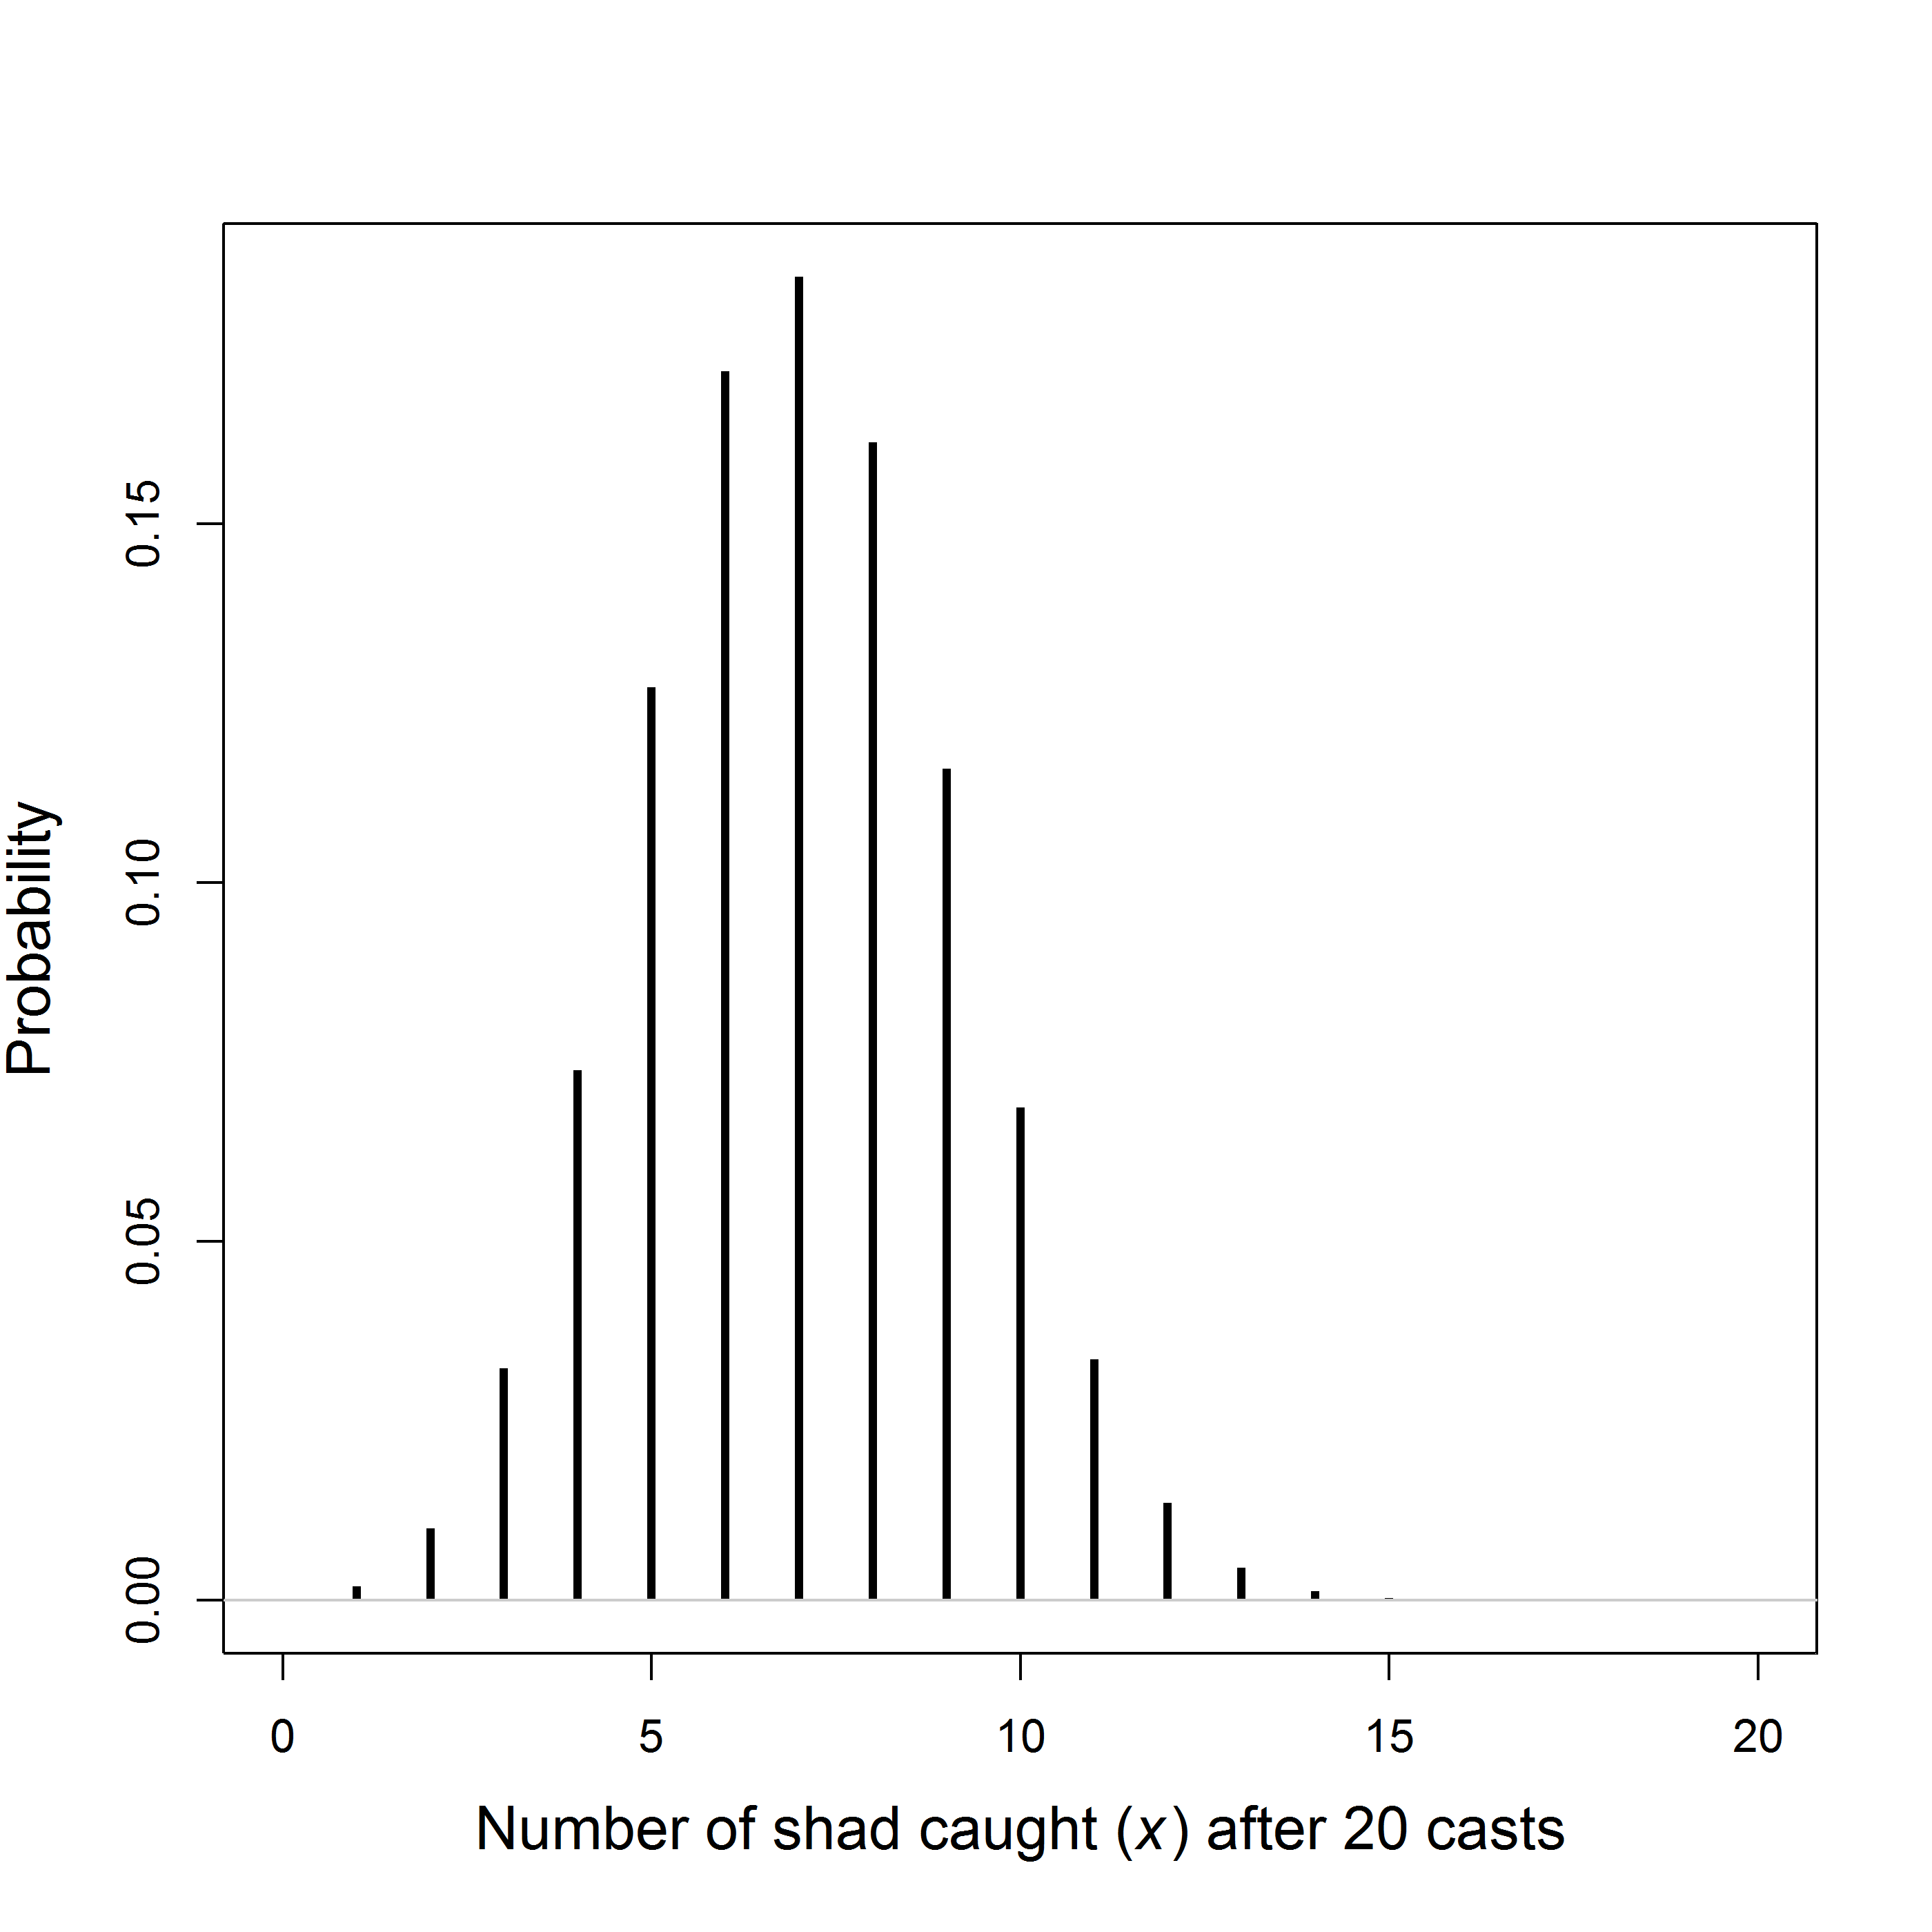
\includegraphics[width=0.65\textwidth]{Ch2/figs/bin}
\caption{The binomial probability mass function with $N=20$ and
  $p=0.35$. }
\label{modeling.fig.bin}
\end{figure}

The purpose of this little example is to show that once we specify a
model for the random variable(s) being studied, we can begin drawing
conclusions, i.e. making inferences, about the processes of interest,
even in the face of uncertainty. Probability distributions are
essential to this process, and thus we need to
understand them in more depth.


%%%% XXXX Add support??
% XXXX Make sideways table?
%\begin{table}%[t!]
\begin{sidewaystable}%[t!]
%  \small
  \caption{Common probability density functions (pdfs) and probability
    mass functions (pmfs) used throughout this book.}
  \begin{tabular}[t]{lcp{4.3cm}ccc}
    \hline
    Distribution & Notation & pmf or pmf & Support & Mean & Variance  \\
                 & & & & $\mathbb{E}(x)$ & Var($x$) \\
    \hline
    \multicolumn{5}{c}{Discrete random variables} \\
    Poisson & $x \sim \text{Pois}(\lambda)$ &
    $\exp(-\lambda)\lambda^x/x!$ & $x \in \{0,1,\ldots\}$ & $\lambda$ & $\lambda$ \\
    Bernoulli & $x \sim \text{Bern}(p)$ & $p^x(1-p)^{1-x}$ & $x \in \{0,1\}$ & $p$ &
    $p(1-p)$  \\
    Binomial & $x \sim \text{Bin}(N, p)$ & $\binom{x}{N}p^x(1-p)^{N-x}$
    & $x \in \{0,1,\ldots,N\}$ & $Np$ & $Np(1-p)$  \\
    Multinomial & $\mathbf{x} \sim \text{Multinom}(N, \bm{\pi})$ &
    $\binom{N}{x_1 \cdots x_k}\pi_1^{x_1} \cdots \pi_k^{x_k}$ & $x_k
    \in \{0,1,\ldots,N\}$ & $N\pi_k$ & $N\pi_k(1-\pi_k)$ \\
    \multicolumn{5}{c}{Continuous random variables} \\
    Normal & $x \sim \text{N}(\mu, \sigma^2)$ & $\frac{1}{\sigma\sqrt{2\pi}}
      \exp(-\frac{(x-\mu)^2}{2\sigma^2})$ & $x \in [-\infty,\infty]$ & $\mu$ & $\sigma^2$  \\
    Uniform & $x \sim \text{Unif}(a, b)$ & $1/(b-a)$ & $x \in [a,b]$ & $(a+b)/2$ &
    $(b-a)^2/12$  \\
%    2D-Uniform & $\mathbf{x} \sim \text{Unif}(\mathcal{S})$ & $1/A(\mathcal{S})$ & &  \\
    Beta & $x \sim \text{Beta}(a, b)$ &
    $\frac{\Gamma(a+b)}{\Gamma(a)+\Gamma(b)}x^{a-1}
    (1-x)^{b-1}$ & $x \in [0,1]$ & $a/(a+b)$ & $\frac{ab}{(a+b)^2(a+b+1)}$ \\
    Gamma & $x \sim \text{Gamma}(a,b)$ &
    $\frac{b^a}{\Gamma(a)}x^{a-1}\exp(-bx)$ & $x\in [0,\infty]$ & $a/b$ & $a/b^2$  \\
    Multivariate Normal & $\mathbf{x} \sim \text{N}(\bm{\mu}, \bm{\Sigma})$ &
    $(2\pi)^{-\frac{k}{2}}|\bm{\Sigma}|^{-\frac{1}{2}}\exp(-\frac{1}{2}(\mathbf{x}-\bm{\mu})'\times\bm{\Sigma}^{-1}(\mathbf{x}-\bm{\mu}))$
    & $x_k \in [-\infty,\infty]$ & $\bm{\mu}$ & $\bm{\Sigma}$ \\
    \hline
  \end{tabular}
  \label{modeling.tab.pdfs}
\end{sidewaystable}
%\end{table}




\subsection{Properties of probability distributions}

A pdf or a pmf is a function like any other function
%Probability distributions are functions like any other functions
in the sense that it has one or more arguments whose values determine
the result of the function. However, probability functions have a few
properties that distinguish them from other functions.
The first is that the function
must be non-negative for all possible values of the random variable,
i.e. $[x] \geq 0$. The second requirement is that the integral of
a pdf must be unity, $\int_{-\infty}^{\infty} [x]\, \text{d}{x} = 1$, and similarly
for a pmf, the summation over all possible values is unity, $\sum_x [x]
= 1$. The following \R~code demonstrates
this for the normal and binomial distributions:
%\begin{samepage}
\begin{verbatim}
> integrate(dnorm, -Inf, Inf, mean=0, sd=1)$value
[1] 1
> sum(dbinom(0:5, size=5, p=0.1))
[1] 1
\end{verbatim}
%\end{samepage}
This requirement is important to remember when one  develops a
non-standard probability distribution. For example, in Chapt.
\ref{chapt.state-space} and \ref{chapt.rsf},
we work with resource selection functions whose probability
density function is not one that is pre-defined in software packages
such as \R~or \bugs.

Another feature of probability distributions is that they can be used
to compute important summaries of random variables. The two most
important summaries are the expected value, $\mathbb{E}(x)$,
and the variance $\text{Var}(x)$. The expected value
can be thought of as the average
of a very large sample from the specified distribution. For
example,
one way of approximating the expected values of a binomial
distribution with $K=20$ trials and $p=0.35$ can be implemented in \R~using:
\begin{verbatim}
> mean(rbinom(10000, 20, 0.3))
[1] 6.9865
\end{verbatim}
For most probability distributions used in this book, the expected
values are known exactly, as shown in Table~\ref{modeling.tab.pdfs}, and
thus we don't need to resort to such Monte Carlo approximations. For instance, the
expected value of the binomial distribution is exactly $\mathbb{E}(X) = Kp =
20 \times 0.35 = 7$. In this case, it happens to take an integer
value, but this is not a necessary condition, even for discrete random
variables.

A more formal definition of an expected value is the average of all
possible values of the random variable, weighted by their
probabilities. For continuous random variables, this weighted average
is found by integration: %{\bf XXXX here I put a * for
%  multiplication. Maybe could have a hard space in there to seperate
%  the two pieces XXXXX}
\begin{equation}
  \mathbb{E}(x) = \int_{-\infty}^{\infty} x \times [x] \, \text{d}{x}.
  \label{modeling:eq:EXc}
\end{equation}
For example, if $[x]$ is normally distributed with mean 3 and unit
variance, we could find the expected value using the following code.
\begin{verbatim}
> integrate(function(x) x*dnorm(x, 3, 1), -Inf, Inf)
3 with absolute error < 0.00033
\end{verbatim}
Of course, the mean \textit{is} the expected value of the normal
distribution, so we didn't need to compute the integral but, the
point is, that Eq.~\ref{modeling:eq:EXc} is generic. For discrete
random variables, the expected value is found by summation rather than
integration: %{\bf XXXX same here XXXXX}
\begin{equation}
  \mathbb{E}(x) = \sum_{x} x \times [x]
  \label{modeling:eq:EXd}
\end{equation}
where the summation is over all possible values of $x$.
Earlier we
approximated the expected value of the binomial distribution
with $K=20$ trials and $p=0.35$ by taking a Monte Carlo
average. Eq.~\ref{modeling:eq:EXd} let's
find the exact answer,  using this bit of \R~code:
\begin{verbatim}
> sum(dbinom(0:100, 20, 0.35)*0:100)
[1] 7
\end{verbatim}
This is great. But of what use is it? One very
important concept to understand is that when we fit
%(generalized linear)
models, we are often modeling changes in the expected value of some random
variable. For example, in Poisson regression, we model its expected
value, say $\lambda$,
which may be a function
of environmental variables.

The ability to model the expected value of a random variable gets us
very far, but we also need sometimes a model for the variance of the random
variable. The variance %is itself a type of expected value; one that
describes the amount of variation around the expected
value. Specifically, $\text{Var}(x) = \mathbb{E}((x -
\mathbb{E}(x))^2)$. Clearly, if the variance is zero, the variable is
not random as there is no uncertainty in its outcome.
For some distributions, notably the normal distribution, the variance
is a parameter to be estimated. Thus, in ordinary linear regression,
we estimate both the expected value $\mu=\mathbb{E}(x)$,
which may be a function of covariates, and the variance
$\sigma^2$, or similarly the residual standard error $\sigma$. For
other distributions, the variance is not an explicit parameter to be
estimated, and instead, the mean to variance ratio is fixed. In the
case of the Poisson distribution, the mean is equal to the
variance, $\mathbb{E}(x) = \text{Var}(x) = \lambda$.
%This is often viewed as a restriction because in ecology
%count data often have a variance greater than the mean. However, much
%of this variation can be ``explained'' by modeling the mean as a
%function of covarites. Still, in cases where extra-Poisson variation
%exists, other distributions such as the negative binomial or
%zero-inflated Poisson distribution may be required.
A similar
situation is true for the binomial distribution---the variance is
determined by the two parameters $K$ and $p$, $\text{Var}(x) = Kp(1-p)$. Thus
in our earlier example with $K=20$ and $p=0.35$, the variance is
4.55. Toying around with these ideas using random number generators
may be helpful. Here is some code to illustrate some of these basic concepts:
\begin{verbatim}
> 20*0.35*(1-0.35)             # Exact variance, Var(x)
[1] 4.55
> x <- rbinom(100000, 20, 0.35)
> mean((x-mean(x))^2)          # Monte Carlo approximation
[1] 4.545525
\end{verbatim}



\section{Common Probability Distributions}
\label{sec.modeling.distributions}

We got a little ahead of ourselves in the previous sections by using
the binomial and Poisson distributions without describing them in detail.
A solid understanding of the binomial, Poisson, multinomial, uniform,
and normal (or Gaussian)
distributions is absolutely essential throughout the
remainder of the book. We will occasionally make use of other
distributions such as the %normal (or Gaussian),
beta, log-normal, %multivariate-normal,
gamma, Dirichlet, etc$\dots$ that can be helpful when
modeling capture-recapture data, but these distributions can be
readily understood once you are comfortable with the more commonly
used distributions described in this section.

\subsection{The binomial distribution}

The binomial distribution plays a critical role in ecology. It is
used for purposes as diverse as modeling count data, survival
probability, occurrence probability, and capture probability, just to
name a few.
To describe the properties of the binomial distribution, and related
distributions, we will introduce a new example.
Suppose we are conducting a bird survey at a site in which $N=10$
chestnut-sided warblers (\textit{Stetophaga pensylvanica}) occur, and
each of these individuals has a detection probability of $p=0.5$. The
binomial distribution is the natural choice for describing the number
of individuals that we would expect to detect ($n$) in this
situation, and using our notation, we can write the model as: $n \sim
\text{Binomial}(10, 0.5)$. Note that if $p \equiv 1$ and we visit the
site on $K$ occasions, the observations $\{n_1, \ldots, n_K\}$
would not be random outcomes---we would always observe
$n_k=10$. That is, the observed data would exactly equal the expected
value and the variance would be zero.
However, when $p<1$, we can expect that we will observe
a different number of warblers on each replicate visit. To see this,
we can simulate data under this simple model with $K=3$ survey occasions
\begin{verbatim}
> n <- rbinom(3, size=10, prob=0.5) # Generate 3 binomial outcomes
> n                                 # Display the 3 values
[1] 6 4 8
\end{verbatim}
The vector of counts will typically differ each time you issue this
command; however, we know the probability of observing any value of
$n_k$ because it is defined by the binomial pmf. As we demonstrated
earlier, in \R~this probability can be found using the \verb+dbinom+
function. For example, the probability of observing $n_k=5$ is given by:
\begin{comment}
  Without knowing a thing about probability distributions, most people
  would recognize that the expected value of $x_j$ is $10 \times 0.5 =
  5$. That is, the most likely number of chestnut-sided warblers that
  we would expect to detect is 5. In this case, however, we did not
  observe a single 5, but rather observed counts of 6, 4, and 8
  chestnut-sided warblers on the first, second, and third surveys
  respectively. If 5 is the most likely outcome, how likely was it to
  observe these data? And what is the actual probability of observing
  a 5? These questions can all be answered by the probability mass
  function (pmf) for the binomial distribution.

  The probability of
  observing a 5 (or any other number) when $N=10$ and $p=0.5$ can be
  computed in \R~by issue the following command:
\end{comment}
\begin{verbatim}
dbinom(5, 10, 0.5)
\end{verbatim}
This simply evaluates the function shown in
Table~\ref{modeling.tab.pdfs}. We could do the same more transparently, but
less efficiently, using any of the following:
\begin{verbatim}
n <- 5; N <- 10; p <- 0.5
factorial(N)/(factorial(n)*factorial(N-n))*p^n*(1-p)^(N-n)
exp(lgamma(N+1) - (lgamma(n+1) + lgamma(N-n+1)))*p^n*(1-p)^(N-n)
choose(N, n)*p^n*(1-p)^(N-n)
\end{verbatim}
Note that the last three lines of code differ only in how they compute the
binomial coefficient $\binom{N}{n}$, which is the number of different ways
we could observe $n=5$ of the $N=10$ chestnut-sided warblers at the site. The
binomial coefficient, which is read ``N choose n'' is defined as
\begin{equation}
  \label{eq:1}
  \binom{N}{n} = \frac{N!}{n!(N-n)!}.
\end{equation}

Now that we know how to simulate binomial data and compute the
probabilities of observing any particular outcome $n$, conditional on the
parameters $N$ and $p$, we can contemplate the relevance of the
binomial distribution in spatial capture-recapture models. One
important application of the binomial distribution is as a model encounter
frequencies. Indeed, one of the most important encounter models in SCR
will be referred to as the ``binomial encounter model'', in which
% For example, suppose that we operate an array of hair snares for
% $K=4$ survey occasions. In this case, an individual can be
% encountered at most once at a snare during a single occasion (because
% multiple distinct hair deposits cannot be distinguished), but the
% individual can be encountered at multiple snares during an occasion as
% it moves about its home range. If there are no time-varying, or
% occasion-specific, covariates then a natural model for
the number of times individual $i$ is captured at ``trap'' $j$ after
$K$ survey occasions is
modeled as $y_{ij} \sim \text{Binomial}(K, p_{ij})$. Here, $p_{ij}$ is the
encounter probability determined, in part, by the distance between an
animal's activity center and the trap location, as will be described
more fully in subsequent chapters. The important point to note is
that $y_{ij}=0$ if individual $i$ is never encountered at trap $j$,
and $y_{ij}=4$ if it is encountered on all four occasions. This
binomial encounter model is
described in detail in Sec.~\ref{scr0.sec.binomial}.
Another important application of the binomial distribution is as a
prior for the population size parameter in Bayesian analyses, as is
discussed in Chapt.~\ref{chapt.closed}.
% , is somewhat advanced, but
% here we simply note that one must choose a prior distribution for $N$.
% In likelihood analysis a Poisson prior is often used, but when
% conducting a Bayesian analysis, we typically use a practice known as
% data augmentation that results in the prior distribution: $N \sim
% \text{Binomial}(M, \psi)$ where $M$ is an arbitrarily large integer,
% and




\subsection{The Bernoulli distribution}

%{\bf XXXX Should this come before the binomial? XXXXX}
% ANDY, I guess it could go either way, but I prefer going from
% general to specific in this case. Same goes for multinomial -> categorical

Above, we showed three alternatives to \verb+dbinom+ for evaluating the
binomial pmf. These three commands differed only in how they computed
the binomial coefficient, which we needed because of the numerous ways
in which we could observe $n=5$ given $N=10$. To conceptualize
this, let $y_i$ be a binary variable indicating if individual $i$
was detected or not. Hence, given that 5 individuals were detected,
the vector of individual detections could be something like
$\mathbf{y}=(0,0,1,1,1,1,1,0,0,0)$, which would indicate
that we detected individuals 3-7 but not 1-2 or 8-10. For $N=10$ and
$n=5$, the binomial coefficient tells us that there
are 252 possibilities of vectors $\mathbf{y}$ that have 5 ones. However, when $N \equiv 1$, this term
drops from the pmf and the result is the pmf for the Bernoulli
distribution. That is, the Bernoulli distribution is simply the
binomial distribution when $N \equiv 1$. Alternatively, we could say that the binomial
distribution is the outcome of $N$ $iid$ Bernoulli trials. We use the
standard term ``$iid$'' to mean {\it independent, identicially distributed}.
%% DEFINE iid here?

The utility of the Bernoulli distribution is evident when we imagine
that not all of the chestnut-sided warblers have the same detection
probability. Thus, if some individuals can be detected with
probability 0.3 and others have a 0.7 detection probability, then the
model $n \sim \text{Binomial}(N, p)$ is no longer an accurate
description of system since $p$ is no
longer constant for all individuals. %%%%a scalar, i.e. a single value.

%% FIXME: Need to clean up notation of $J$ visits

To properly account for variation in $p$, we could redefine our model
for the %our notation
%describing how the
counts of chestnut-sided warblers as
%are generated. Our model now is
\begin{gather}
y_{ik} \sim \text{Bernoulli}(p_i) \nonumber \\% \;\; \text{for} \; i=1,2,\dots,N \\
n_k = \sum_{i=1}^N y_{ik}
\label{modeling.eq.Bern}
\end{gather}
This  states that individual $i$ is detected with probability
$p_i$, and the observed count is the sum of the $N$ Bernoulli
outcomes.

An important point is that the individual-specific data $y_{ik}$ can only be
observed  {\it if} the individuals are uniquely distinguishable, such as when they
are marked by biologists with color bands, or by boy-biologists with
paint-ball guns.
%Indeed, this is one of the important
%motivations for capture-recapture studies.
In such cases, the Bernoulli distribution allows us to
model variation in detection probability among individuals and thus
would be preferable to the binomial distribution, which assumes that each
of the $N$ individuals have the same $p$.
For this reason, the Bernoulli
distribution, as simple as it is, is of paramount importance in
capture-recapture models, including spatial capture-recapture models
in which there is virtually always substantial and important variation in capture probability
among individuals. Indeed, it could be said the Bernoulli model is the
canonical model in capture-recapture studies, and most of the
different flavors of capture-recapture models differ primarily in how $p_i$ is
specified. % and how $N$ is estimated.

The Bernoulli pmf is given by  $p^n(1-p)^{1-n}$ and hence we do not need canned
functions to facilitate its evaluation. Of course, if you wanted to, you
could always use \verb+dbinom+ with the \verb+size+ argument set to
1, e.g. \verb+dbinom(1, 1, 0.3)+ returns the Bernoulli probability of
observing $n=1$ given $p=0.3$.

\subsection{The multinomial and categorical distributions}
\label{modeling.sec.multinom}

The binomial distribution is used
when we are accumulating a binary response -- that is, one in which
there are two possible categories, such as success/failure or
captured/not-captured.
The multinomial distribution is a multivariate extension of
the binomial used when there are $G>2$ categories.
The multinomial distribution can be thought of as a model for placing
$N$ items in the $G$ categories, which are also called bins or cells. Each bin has
its own probability $\pi_g$ and these probabilities must sum to one.
In ecology, $N$ is often population size or the number of individuals
detected, but the definition of the $G$ bins varies among
applications. For example, in distance sampling, when the distance
data are aggregated into intervals,
the bins are the distance intervals, and the cell probabilities are
functions of detection probability in each interval \citep{royle_etal:2004}.

The multinomial distribution is widely used to model data from traditional,
non-spatial capture-recapture studies.
Earlier we let $y_{ik}$ denote a binary random variable indicating if
warbler $i$ was detected on survey $k$. The vector of observations for an
individual, $\mathbf{y}_i$, is often referred to as the individual's
``encounter history''. The number of possible encounter
histories depends on the number of survey occasions. Specifically,
there are $2^K$
possible encounter histories\footnote{When $N$ is unknown, we can
  never observe the ``all-0'' encounter history, corresponding
to an individual that is not
  detected, and thus the number of ``observable'' encounter histories
  is $2^{K-1}$}.
If we tabulate the number of individuals with each encounter history,
the frequencies can be modeled using the multinomial
distribution. %, as we will soon explain.

Going back to our
chestnut-sided warbler example, suppose the 10 individuals are marked
and we make $K=2$ visits to the site such that there are $2^K = 4$ possible encounter
histories: $(11, 10, 01, 00)$, where, for example,  ``10'' is the
encounter history for an individual detected on the first visit but not
the second. If $p=1$, then the
encounter history for each of the 10 individuals must  be ``11''. That
is, we would detect each individual on both occasions. In this case,
we could format our data as $\mathbf{h} = (10, 0, 0, 0)$. The
corresponding cell probabilities would be $\bm{\pi} = (1, 0, 0,
0)$. What about the situation where $p<1$, e.g. $p=0.3$? In this case, the
probability of observing the capture history ``11'' (detected on both
occasions) is $p \times p = 0.3 \times 0.3 = 0.09$. The probability of
observing ``10'' is $p \times (1-p) = 0.21$. Following this logic, the vector
of cell probabilities is $\bm{\pi} = (0.09, 0.21, 0.21, 0.49)$. We can
simulate data under this model as follows:
\begin{verbatim}
> caphist.probs <- c("11"=0.09, "10"=0.21, "01"=0.21, "00"=0.49)
> drop(rmultinom(1, 10, caphist.probs))
11 10 01 00
 0  3  2  5
\end{verbatim}
(the \verb+drop+ function simply converts the matrix to a vector).
The
result of our simulation is that zero individuals were observed with
the capture history ``11'' and 5 individuals were observed with the
capture history ``00''. The other 5 individuals were observed one out
of the two occasions. This is not such a surprising outcome given
$p=0.3$.
%Note that the a single outcome of a multinomial distribution
%is a vector, and hence it is a multivariate distribution in contrast
%to the univariate distributions discussed so far.

As in non-spatial capture-recapture studies, the multinomial
distribution turns out to be very important in spatial
capture-recapture studies. However, $N$ is not defined as population
size. Rather, we use the multinomial distribution when an individual
can only be captured in a single trap during an occasion. Thus
$N=1$ and the cell probabilities are the probabilities of
being captured in each trap. A thorough discussion of this point can
be found in Chapt.~\ref{chapt.poisson-mn}. Another application of the
multinomial distribution in SCR models is discussed in
Chapt.~\ref{chapt.state-space} where we discuss how to model the
probability that an individual's activity center is located in one of
the cells of a raster defining the spatial region of interest.

%It is worth noting that,
Just as the Bernoulli distribution is the elemental form of the
 binomial distribution (being the case $N=1$), the
categorical distribution is essentially equivalent to
%special case of
the multinomial distribution with size parameter
$N\equiv1$. The only difference is that, rather than returning a
vector with a single element equal to 1, it returns the element number
where the 1 occurs. For example, if $\mathbf{y}=(0,0,1,0)$ is an outcome of a
multinomial distribution with $N=1$, then the categorical outcome
would be 3 because the 1 is located in third position in the vector. Thus, in spatial
capture-recapture models, we might use either the multinomial
distribution with $N=1$ or %we can just as well use
the categorical distribution. %They are equivalent.
The various {\bf BUGS} engines describe the categorical distribution
by the declaration \mbox{\tt dcat} and, in {\bf R}, we can simulate
categorical outcomes using the function \mbox{\tt sample}.


\subsection{The Poisson distribution}


The Poisson distribution is the canonical model for count data in
ecology.  More generally, the
Poisson distribution is a model for random variables taking on
non-negative, integer values.  Although it is a simple model having just one
parameter, $\lambda = \mathbb{E}(x) = \text{Var}(x)$, its applications
are highly diverse, including
as a model of spatial variation in abundance or as a model for the
frequency of behaviors over time.  Just as logistic regression is the
standard generalized linear model (GLM) used to model binary data, Poisson
regression is the default GLM for modeling count data and variation in
$\lambda$.

The Poisson distribution is related to
both the binomial and multinomial distributions, and the following two
bits of trivia are occasionally worth knowing. First, it is the limit of the binomial
distribution as $N \to \infty$ and $p \to 0$, which means that for
high values of $N$ and low values
of $p$, $\text{Poisson}(N\times p)$ is approximately equal to $\text{Binomial}(N,
p)$. Second, if $\{n_1 \sim \text{Poisson}(\lambda_1),
%n_k \sim \text{Poisson}(\lambda_k),
\dots, n_K \sim \text{Poisson}(\lambda_K)\}$
then the vector of counts is multinomial, $\{n_1, \dots, n_K\}
\sim \text{Multinomial}(\sum_k n_k, \{\frac{\lambda_1}{\sum_k \lambda_k},
%\frac{\lambda_k}{\sum_{n_k} \lambda_k},
\dots, \frac{\lambda_K}{\sum_k \lambda_k}
\})$.

The Poisson distribution has two important uses in spatial
capture-recapture models: (1) as a prior distribution for the
population size parameter $N$, and (2) as a model for the frequency of
captures in a trap. In the first context, the Poisson prior for $N$
results in a Poisson point process for the location of the $N$
activity centers in the region of interest. This topic is discussed
in-depth in Chapt.~\ref{chapt.scr0} and Chapt~\ref{chapt.state-space}.
% point process model, which is a
% spatially-explicit extension of the simple Poisson model.
% If $N$ individuals are uniformly distributed in some region
% $\mathcal{S}$ with area $A$, and $N$ is a Poisson
% random variable, we call this the homogeneous Poisson point process
% whose intensity parameter is $\lambda = 1/A$. The intensity parameter
% is defined as the expected number of points that one would find in an
% infinitesimally small area. Often, the intensity parameter is not
% constant, but rather it takes on different values for each location
% $x$ in the region $\mathcal{S}$. The inhomogeneous Poisson point
% process model can be useful in such cases, and typically, the
% intensity is modeled as a log-linear function of spatially-referenced
% environmental covariates. Thus, rather than $\lambda$, the intensity
% parameter is now $\lambda(x)$. Inhomogeneous Poisson point process
% models have a long history of applications in forestry, and are now
% being increasingly used to model species distributions. They are also
% extremely important in spatial capture-recapture as we will soon see.
% Under the homogeneous Poisson point process model,
% the number of individuals occurring in some
% region $B \in A$ is Poisson distributed with expectation
% $\lambda = N/A$. As before, $\lambda$ might vary among regions, which
% might be distinct habitat patches or arbitrarily-defined survey plots or
% quadrats and Poisson regression could be used for inference.
The second use of the Poisson distribution in spatial capture-recapture is
to describe data from sampling methods in which an
individual can be detected multiple times at a trap during a single
occasion. For example, in camera trapping studies we might obtain
multiple pictures of the same individual at a trap during a single sampling
occasion. Thus, $\lambda$ in this case would be defined as the
expected number of detections or captures per occasion.


\subsection{The uniform distribution}

The %first continuous distribution we will describe is the
lowly uniform distribution is a continuous distribution whose
only two parameters are the lower and upper bounds that restrict the
possible values of the random variable $x$. These bounds
are almost always known, so there is typically nothing to
estimate. Nonetheless, the uniform
distribution is one of the most widely used distributions,
especially among Bayesians who frequently use it to as a ``non-informative''
prior distribution for a parameter. For example, if we
have a capture probability parameter $p$ that we wish to estimate, but
we have no prior knowledge of what value it may take in the range
[0,1], we will often use the prior $p \sim \text{Uniform}(0,1)$. This
states that $p$ is equally likely to take on any value between
zero and one.

Another common usage of the uniform distribution is as a prior for the
%x- and y-
coordinates of points in the real plane, i.e. in two-dimensional
space. Such a use of the uniform distribution implies that a point process is
``homogeneous'', meaning that the location of one point does not
affect the location of another point and that the expected density of
points is constant throughout the region. Thus, to simulate a
realization from a homogeneous Poisson point process in the unit square
$[0,1] \times [0,1]$, we could use the following \R~code:
\begin{verbatim}
D <- 100    # points per unit area
A <- 1      # Area of unit square
N <- rpois(1, D*A)
plot(s <- cbind(runif(N), runif(N)))
\end{verbatim}
where \verb+s+ is a matrix of coordinates with $N$ rows and 2 columns. We
will often represent the uniform point process using the following notation:
\begin{equation}
  {\bf s} \sim \text{Uniform}(\mathcal{S})
\end{equation}
where ${\cal S}$ is some specific unit of space called the state-space
of the random variable ${\bf s}$.
It would be more correct to somehow distinguish this
two-dimensional uniform distribution for the univariate one. That is,
it might be more clear to use notation such as
${\bf s} \sim \text{Uniform}_2(\mathcal{S})$ instead, but this is somewhat
cumbersome, so we will opt for the former expression.


%\subsection{The Normal and Bivariate Normal Distributions}
\subsection{Other distributions}

The other continuous distributions that are regularly encountered in SCR
models are
primarily used as priors in Bayesian analyses, and thus we will avoid
a lengthy discussion of their properties. %The  we will briefly
%cover here are the beta and gamma distributions, which are
%particularly useful as priors for probabilities and positive-valued
%parameters respectively. Although we will keep it very brief, note that
%Table~\ref{modeling.tab.pdfs} includes
%the pdfs, expected values, and variances of these distributions.
%A more thorough treatment of
%these distributions can be found in \citet{link_barker:2010}.
%This might seem odd given that
%standard statistics courses taken by ecologists focus heavily on the normal
%distribution. However, in capture-recapture studies, we rarely observe
%random variables that are continuous,
%and hence, we will just briefly
%mention the normal, beta, and gamma distributions.
%Once upon a time, ecologists modeled just about everything as normally
%distributed. One reason for this is that methods such a linear
%regression and $t$-tests were all that were available in many
%primitive stats software programs. Another reason why
The normal distribution, also called the Gaussian
distribution, is perhaps the most widely recognized and applied probability model in
statistics, but it plays only a minor role in SCR models although it
has been used as a model for signal strength in acoustic SCR models
\citep{efford_etal:2009ecol,dawson_efford:2009}, and see Sec. \ref{poisson-mn.sec.acoustic}. %The reason
%being that many of the random variables in SCR models are discrete,
%and distinctly not normally distributed.
Nonetheless, it
is the canonical prior for any continuous random variable with
infinite support, and thus it is often used as a prior when applying Bayesian
methods. One common usage is as a prior for the $\beta$
coefficients of a linear model defining some parameter as a function
of covariates (usually on a transformed scale). An example, including a
cautionary note, is provided in Sec.~\ref{glms.sec.choice}.
Be aware that although the normal distribution is typically
parameterized in terms of the variance parameter $\sigma^2$, in
the \bugs~language, the inverse of the variance, or precision, is used
instead, $\tau = 1/\sigma^2$.

The bivariate normal distribution is a generalization of the
normal distribution and a special case of the multivariate normal
distribution whose pdf is shown in Table~\ref{modeling.tab.pdfs}. The
bivariate normal distribution is used to model two (possibly) dependent
continuous variables whose symmetric variance-covariance matrix is
denoted $\bm{\Sigma}$.
%The parameter $\rho$ is two off-diagonals of this matrix are
In SCR models, we most often use this model as
a rudimentary description of movement outcomes about a home range
center. If there is there is no correlation, then the model reduces to
two independent normal draws along the coordinate axes. The following code generates bivariate normal
outcomes with no correlation ($\rho=0$, the object \verb+X1+) and with
$\rho=0.9$, the object \verb+X2+.
\begin{verbatim}
library(mvtnorm)
set.seed(3)
mu <- c(0,0)
Sigma <- matrix(c(1, .9, .9, 1), 2, 2)
X1 <- cbind(rnorm(50, mu[1], Sigma[1,1]), # No correlation (rho=0)
            rnorm(50, mu[2], Sigma[2,2]))
X2 <- rmvnorm(50, mu, Sigma)              # rho=0.9
\end{verbatim}
Fig.~\ref{modeling.fig.bvn} shows the simulated points.
\begin{figure}
  \centering
  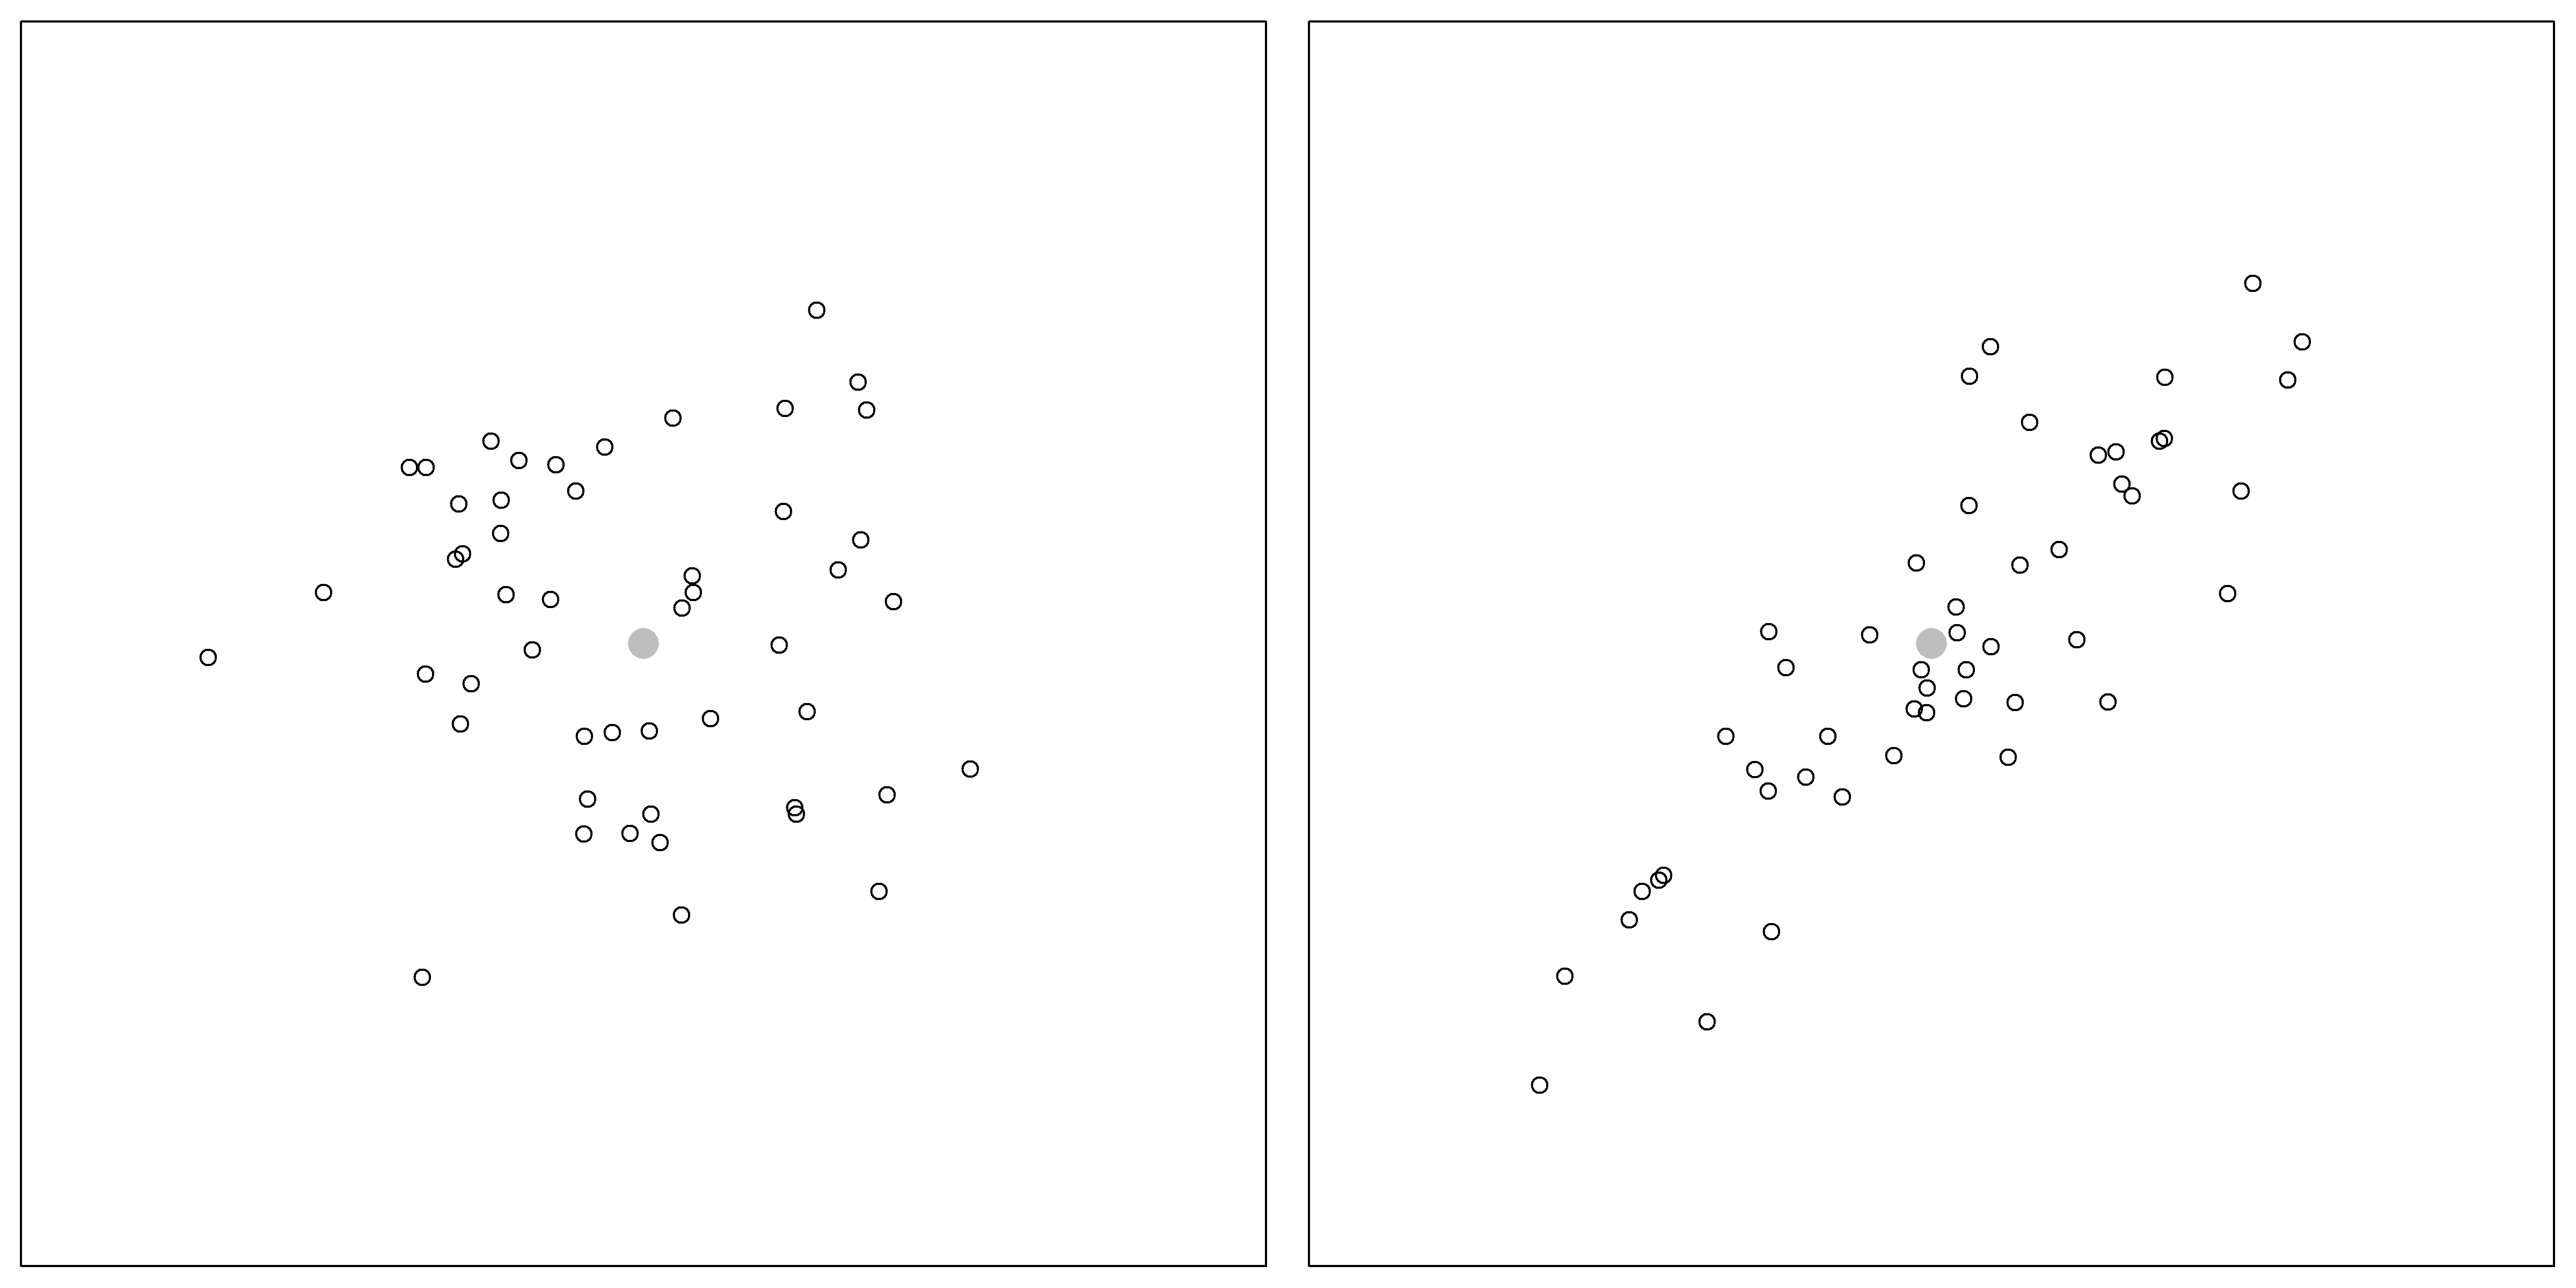
\includegraphics[width=0.9\textwidth]{Ch2/figs/bvn}
  \caption{Two realized point patterns from the bivariate normal distribution. }
  \label{modeling.fig.bvn}
\end{figure}

Several of the parameters in capture-recapture models do not have
infinite support, but are instead are
probabilities restricted to the range $[0,1]$, or are positive valued
living between zero and $\infty$. The beta distribution is the
standard prior used for probabilities because it can be used to express either a
lack of knowledge or very precise knowledge about a
parameter. For example, a $\text{Beta}(1,1)$ distribution is
equivalent to a $\text{Uniform}(0, 1)$ distribution. However, unlike the
the uniform distribution, the beta distribution can be used as an
informative prior; for example if published estimates of detection
probability exist we can choose parameters of the beta distribution to
reflect that. To gain some familiarity with the beta
distribution, execute the following \R~commands:
\begin{verbatim}
curve(dbeta(x, 1, 1), col="black", ylim=c(0,5))
curve(dbeta(x, 10, 10), col="blue", add=TRUE)
curve(dbeta(x, 10, 20), col="darkgreen", add=TRUE)
\end{verbatim}

Other parameters in SCR models are continuous but
positive-valued and can be modeled using the gamma distribution. As
with the beta distribution, the gamma distribution is typically
favored over the uniform distribution when one is interested in using
an informative prior. It is also frequently used as a vague prior for
the inverse of
variance parameters, but it is wise to compare this prior to a uniform
to assess its influence on the posterior.

\section{Statistical Inference and Parameter Estimation}

If the parameters of a statistical model were known with absolute
certainty, then it would be possible to
%could ignore statistial inference a
use pdfs and pmfs to make direct
probability statements about unknowns such as future outcomes. However, we
almost never know the actual values of parameters, and instead we have
to estimate them from observations (i.e., data). Our inferences must then acknowledge the uncertainty
associated with our imperfect knowledge of the parameters. Doing so is
most often accomplished using one of two approaches:
classical (frequentist) inference or Bayesian
inference.
%Both types of statistical inference make heavy use of
%probability distributions.
These two modes of inference
regard the uncertainty about parameters in
entirely different ways. In the next chapter, we will review some of
the important concepts in Bayesian inference, so here, we will
focus on the frequentist perspective.

%In classical inference, if
Suppose  we count oak trees at
$J$ sites, and the resulting data $\{y_1, \ldots, y_J\}$ can be
assumed to be iid outcomes from some %  we want to know the average number of oaks
%per site. We might assume that the counts are distributed according to some
distribution, such as the Poisson with unknown parameter $\lambda$. We
want to estimate this parameter. %,
%which is the parameter we need to estimate.
In classical inference, the only uncertainty about $\lambda$ %that we are concerned with
is that attributable to
sampling. For instance, we can imagine repeatedly sampling the
population (sites in this example) and obtaining sample-specific estimates of
$\lambda$. Typically, we entertain the idea that there are an infinite
number of possible samples and so we could obtain an infinite
number of estimates: \{$\hat{\lambda}_1, \hat{\lambda}_2, \hdots,
\hat{\lambda}_\infty\}$. If
these estimates are produced using the method of maximum likelihood,
the distribution of estimates, called the sampling distribution, will
be normally distributed with $\mathbb{E}(\hat{\lambda})=\lambda$. The
standard deviation of the sampling distribution is called the standard
error, which can  be estimated as part of the maximum likelihood
procedure. Given $\hat{\lambda}$ and an estimate of its standard
deviation, we can construct a confidence interval
that will include the true value of $\lambda$  with some prescribed
coverage probability.
%which will tend toward zero as the sample size $J$ increases toward
%infinity. In other words, if the sample size is large, the estimate
%will always be close to the actual parameter value. Maximum likelihood
%is a method of estimating both $\lambda$ and the standard error (or
%variance) of lambda.
%variance of the sampling distribution
%{\bf XXXX not sure sampling distribution was defined yet XXXXX}
%will approach zero as the size of the sample increases towards
%infinity.
Note that there is
no uncertainty associated with the actual parameter---it is regarded
as a fixed value, and hence probability is only used to characterize
the estimator via its sampling distribution.

Maximum likelihood is heuristically a method of finding the most ``likely''
value of $\lambda$, given the observed data, and of characterizing the
variance of the sampling distribution. Of course, it also applies to
cases where the observations are multivariate, or the probability
distribution is a function of multiple parameters. Endless numbers of
textbooks and online resources are available for those interested in a
detailed explanation of maximum likelihood. For our purposes, we wish
to keep it simple and focus on \textit{how} to do it. The first step
is to define the likelihood function, which is
is the joint distribution of the data regarded as a function of
the parameter(s). If the joint distribution of the observations is
denoted by $[y_1, y_2, \dots, y_n | \lambda]$, we usually denote the
likelihood by flipping the arguments:
$\mathcal{L}(\lambda | \mathbf{y}) = [\lambda | y_1, y_2, \dots, y_n]$.

If the observations are $iid$, the likelihood simplifies to
\begin{equation}
  \mathcal{L}(\lambda | \mathbf{y}) = \prod_i [y_i | \lambda].
  \label{modeling.eq.like}
\end{equation}
where $[y_i | \lambda]$ is a probability distribution, like those
discussed in the previous sections. For example, if $y_i$ is
Poisson distributed, then
$[y_i | \lambda] = \text{Poisson}(\lambda) = \frac{\lambda^{y_i}e^{-\lambda}}{y_i!}$.
Although likelihoods are typically shown on the natural scale, we
almost always maximize the logarithm of the likelihood to
avoid computational problems that arise when multiplying very small
probabilities. Thus, we rewrite~\ref{modeling.eq.like} as
\begin{equation}
  \ell(\lambda | \mathbf{y}) = \sum_i \log(f(y_i | \lambda))
  \label{modeling.eq.like2}
\end{equation}
Here is some simple \R~code to simulate independent Poisson outcomes
and estimate $\lambda$ (as though we did not know it) using the
method of maximum likelihood. Actually, we will minimize the negative
log-likelihood because it is equivalent and is the default for \R's
optimizers like \verb+optim+ and \verb+nlm+.
\begin{verbatim}
> lambda <- 3                 # Actual parameter value
> y1 <- rpois(100, lambda)    # Realized values (data)
> negLogLike1 <- function(par) -sum(dpois(y1, par, log=TRUE))
> starting.value <- c(`lambda'=1)
> optim(starting.value, negLogLike1)$par # MLE
  lambda
3.039844
\end{verbatim}
Explicitly maximizing the likelihood, numerically, isn't actually
necessary here because the MLE of
$\lambda$ is given by the  mean of the observations. A more interesting
example is when there are
covariates of $\lambda$. For example, suppose $\lambda$ is a function
of elevation and vegetation height according to: $\log(\lambda_i) =
\beta_0 + \beta_1\texttt{ELEV}_i + \beta_2\texttt{VEGHT}_i$. This is a
standard Poisson regression problem, with likelihood:
\begin{equation}
  \mathcal{L}(\bm{\beta} | \mathbf{y}) = \prod_i \text{Poisson}(y_i | \lambda_i)
  \label{modeling.eq.like3}
\end{equation}
This likelihood is almost identical to the previous one except
that $\lambda$ is now a function, and so we need to estimate the
parameters of the function, i.e. the $\beta$'s. %This class of models is
%known as Poisson regression, a form of a generalized linear model that
%we alluded to earlier.
Some code to fit this model to simulated data is shown here:
\begin{verbatim}
> nsites <- 100
> elevation <- rnorm(100)
> veght <- rnorm(100)
> beta0 <- 1
> beta1 <- -1
> beta2 <- 0
> lambda <- exp(beta0 + beta1*elevation + beta2*veght)
> y2 <- rpois(nsites, lambda)
> negLogLike2 <- function(pars) {
+     beta0 <- pars[1]
+     beta1 <- pars[2]
+     beta2 <- pars[3]
+     lambda <- exp(beta0 + beta1*elevation + beta2*veght)
+     -sum(dpois(y2, lambda, log=TRUE))
+ }
> starting.values <- c('beta0'=0, 'beta1'=0, 'beta2'=0)
> optim(starting.values, negLogLike2)$par
      beta0       beta1       beta2
 0.98457756 -1.03025173 -0.01218292
\end{verbatim}
We see that the maximum likelihood estimates (MLEs) are very close to
the true parameter values.

\begin{comment}
  There are a couple of other basic points to make with respect to
  this example. First, note that, although the log-link is the most commonly used link
  funciton in Poisson regression, many other functions can be
  considered that map the linear predictor (i.e. the righthand side of
  the equation) to the admissible values of the parameter. For example,
  in logistic regression common link distributions include the logit,
  probit, and complementary log-log links. In spatial
  capture-recapture models we often model model capture probability
  using the logit link, although many other options are routinely
  considered. A second think to note is that categorical variables can
  be easily included in the model as covariates. To do so, we simply
  need to create ``dummy variables'' which are combinations of binary
  indicator variables that code each level of the variable.
\end{comment}

In these examples, the parameters we estimated are called fixed
effects by frequentists. Fixed effects are parameters that are not
%themselves
regarded as being random variables.
%\footnote{Thus, technically speaking, there are no such
%  things as fixed effects in Bayesian inference}.
A random effect, in
contrast, is a parameter that can be regarded as the outcome of
a random variable. For instance,
we could entertain the idea that the intercept of our GLM differs
among locations, and that it's actual value is an outcome of a normal
distribution with parameters $\mu$ and $\sigma^2$. In this case,
$\beta_i$ would be a random effect, and our model could be written:
\begin{gather*}
y_i \sim \text{Poisson}(\lambda_i) \\
\log(\lambda_i) = \beta_i + \beta_1\text{ELEV}_i + \beta_2\text{VEGHT}_i \\
\beta_i \sim \text{Normal}(\mu, \sigma^2)
\end{gather*}
This is an example of a mixed effects model or a hierarchical
model. How do we estimate the parameters of a model that includes
random effects? Earlier the likelihood function was written as the
product of probabilities determined by a single pmf or pdf,
$[y|\lambda]$, but now we have an additional random variable, and we
are forced to think about conditional relationships, because $y$
depends upon $\beta_i$ and $\beta_i$ depends upon other parameters,
specifically $\mu$ and $\sigma^2$.
This type of conditional dependence among parameters is the essence of hierarchical
models, and statistical analysis of hierarchical models requires that
we discuss joint distributions, marginal distributions and conditional
distributions.




\section{Joint, Marginal, and Conditional Distributions}

So far we have restricted our attention to situations in which we wish
to make inference about a single random variable.
However, in ecology, we often are interested in multiple random
variables and how they are related.
Let $Y$ be a random variable
%whose realized values
that may or may not be independent of $X$ (here again we will
distinguish between random variables and realized values for
conceptual clarity). Inference
about these two random variables can be made using the joint,
marginal, or conditional distributions---or, we may make use of all of
them depending on the question being asked. In the case of
discrete random variables, the joint
distribution is the probability that $X$ takes on the value $x$
\textit{and} that $Y$ takes on the value $y$, which is written
$[X=x,Y=y]$. To clarify this concept, let's go back to our original
example where $X$ was the number of fish caught after 20 casts, which
we said was an $iid$
binomial random variable. Now,
let's suppose that $X$ depends on the random variable $Y$, which is
the number of other fisherman at the hole. Specifically, let's say
that the probability of catching a fish $p$ is related to $X$
according to $\text{logit}(p) = -0.6 + -2y$. Furthermore, let's
make the intuitive assumption that the number of fishermen at the hole
is a Poisson random variable with mean $0.6$, i.e. $X \sim
\text{Poisson}(0.6)$. Our model is now fully specified, and so we can
answer the question: ``what is the probability of catching $x$ fish
\textit{and} of there being $y$ fishermen at the hole''. This joint
distribution is given by the product of the binomial pmf (with $p$
determined by $y$) and the Poisson pmf with $\lambda=0.6$. The
following \R~code creates the joint distribution.
\begin{small}
\begin{verbatim}
> X <- 0:20  # All possible values of X
> Y <- 0:10  # All possible values of Y
> lambda <- 0.6
> p <- plogis(-0.62 + -2*Y) # p as function of Y
> round(p,2)
 [1] 0.35 0.07 0.01 0.00 0.00 0.00 0.00 0.00 0.00 0.00 0.00
> joint <- matrix(NA, length(X), length(Y))
> rownames(joint) <- paste("X=", X, sep="")
> colnames(joint) <- paste("Y=", Y, sep="")
>
> # Joint distribution [X,Y]
> for(i in 1:length(Y)) {
+     joint[,i] <- dbinom(X, 20, p[i]) * dpois(Y[i], lambda)
+ }
> round(joint,2)
      Y=0  Y=1  Y=2  Y=3 Y=4 Y=5 Y=6 Y=7 Y=8 Y=9 Y=10
X=0  0.00 0.08 0.08 0.02   0   0   0   0   0   0    0
X=1  0.00 0.12 0.02 0.00   0   0   0   0   0   0    0
X=2  0.01 0.08 0.00 0.00   0   0   0   0   0   0    0
X=3  0.02 0.04 0.00 0.00   0   0   0   0   0   0    0
X=4  0.04 0.01 0.00 0.00   0   0   0   0   0   0    0
X=5  0.07 0.00 0.00 0.00   0   0   0   0   0   0    0
X=6  0.09 0.00 0.00 0.00   0   0   0   0   0   0    0
X=7  0.10 0.00 0.00 0.00   0   0   0   0   0   0    0
X=8  0.09 0.00 0.00 0.00   0   0   0   0   0   0    0
X=9  0.06 0.00 0.00 0.00   0   0   0   0   0   0    0
X=10 0.04 0.00 0.00 0.00   0   0   0   0   0   0    0
X=11 0.02 0.00 0.00 0.00   0   0   0   0   0   0    0
X=12 0.01 0.00 0.00 0.00   0   0   0   0   0   0    0
X=13 0.00 0.00 0.00 0.00   0   0   0   0   0   0    0
X=14 0.00 0.00 0.00 0.00   0   0   0   0   0   0    0
X=15 0.00 0.00 0.00 0.00   0   0   0   0   0   0    0
X=16 0.00 0.00 0.00 0.00   0   0   0   0   0   0    0
X=17 0.00 0.00 0.00 0.00   0   0   0   0   0   0    0
X=18 0.00 0.00 0.00 0.00   0   0   0   0   0   0    0
X=19 0.00 0.00 0.00 0.00   0   0   0   0   0   0    0
X=20 0.00 0.00 0.00 0.00   0   0   0   0   0   0    0
\end{verbatim}
\end{small}
This matrix tells us the probability of all possible combinations of
$x$ and $y$, and we see that the most likely value is $(X=1,Y=1)$,
i.e. we will catch 1 fish and there will be 1 other fisherman. This
matrix also demonstrates the law of total probability, which dictates
that the sum of of these probabilities must equal 1.

Perhaps most fisherman don't care about joint distributions, but a
question that might be asked is ``what is the probability
of catching 1 fish today?'' We know that this depends on the
number of fisherman, but we don't know how many will show up
today, so this is a different question than ``what is most likely
value of $X$ and $Y$''. This brings us to the marginal distribution, which is defined by
%{\bf XXXX I think these are wrong. $[X] = \int_{y} [X,Y] = \int_{y}
%  [X|Y][Y]$ etc... XXXXX} %%% FIXED
\begin{equation*}
  [X] = \sum_Y [X,Y] \qquad
  [Y] = \sum_X [Y,X]
\end{equation*}
for discrete random variables, and
\begin{equation*}
  [X] = \int_{-\infty}^\infty [X,Y] \, \mathrm{d}Y \qquad
  [Y] = \int_{-\infty}^\infty [Y,X] \, \mathrm{d}X
\end{equation*}
for continuous random variables. The key idea here is that to get the
marginal distribution of $X$, we have to contemplate all possible
values of $Y$. Computing marginal distributions is a key step in
maximizing likelihoods involving random effects, as will be
demonstrated in Chapt.\ref{chapt.mle}. Here is some \R~code to compute
the marginal distribution of $X$, i.e. the probability of catching
$X=x$ fish:
\begin{verbatim}
> margX <- rowSums(joint)
> round(margX, 2)
 X=0  X=1  X=2  X=3  X=4  X=5  X=6  X=7  X=8  X=9 X=10 X=11 X=12 X=13 X=14
0.18 0.14 0.09 0.05 0.05 0.07 0.09 0.10 0.09 0.06 0.04 0.02 0.01 0.00 0.00
X=15 X=16 X=17 X=18 X=19 X=20
0.00 0.00 0.00 0.00 0.00 0.00
\end{verbatim}
Bad news---the most likely value is $X=0$. However, the chances of
catching 1 fish is pretty similar.

The last type of question we can ask about these two random variables
relates to their conditional distributions. The
conditional probability distribution is the distribution of one
variable, given a realized value of the other. In the case of two discrete random
variables, the conditional distribution may be written as
$[X=x|Y=y]$, i.e. the probability of $X$ taking on the value $x$
given the realized value of $Y$ being $y$. For simplicity, we will
write this as $[X|Y]$. Conditional distributions are defined as follows:
\begin{equation*}
  [X|Y] = \frac{[X,Y]}{[Y]} \qquad [Y|X] = \frac{[X,Y]}{[X]}.
\end{equation*}
That is, the conditional distribution of $X$ given $Y$ is the joint
distribution divided by the marginal distribution of $Y$.
\begin{verbatim}
> XgivenY <- joint/matrix(margY, nrow(joint), ncol(joint), byrow=TRUE)
> round(XgivenY, 2)
      Y=0  Y=1  Y=2  Y=3 Y=4 Y=5 Y=6 Y=7 Y=8 Y=9 Y=10
X=0  0.00 0.25 0.82 0.97   1   1   1   1   1   1    1
X=1  0.00 0.36 0.16 0.03   0   0   0   0   0   0    0
X=2  0.01 0.25 0.02 0.00   0   0   0   0   0   0    0
X=3  0.03 0.11 0.00 0.00   0   0   0   0   0   0    0
X=4  0.07 0.03 0.00 0.00   0   0   0   0   0   0    0
X=5  0.13 0.01 0.00 0.00   0   0   0   0   0   0    0
X=6  0.17 0.00 0.00 0.00   0   0   0   0   0   0    0
X=7  0.18 0.00 0.00 0.00   0   0   0   0   0   0    0
X=8  0.16 0.00 0.00 0.00   0   0   0   0   0   0    0
X=9  0.12 0.00 0.00 0.00   0   0   0   0   0   0    0
X=10 0.07 0.00 0.00 0.00   0   0   0   0   0   0    0
X=11 0.03 0.00 0.00 0.00   0   0   0   0   0   0    0
X=12 0.01 0.00 0.00 0.00   0   0   0   0   0   0    0
X=13 0.00 0.00 0.00 0.00   0   0   0   0   0   0    0
X=14 0.00 0.00 0.00 0.00   0   0   0   0   0   0    0
X=15 0.00 0.00 0.00 0.00   0   0   0   0   0   0    0
X=16 0.00 0.00 0.00 0.00   0   0   0   0   0   0    0
X=17 0.00 0.00 0.00 0.00   0   0   0   0   0   0    0
X=18 0.00 0.00 0.00 0.00   0   0   0   0   0   0    0
X=19 0.00 0.00 0.00 0.00   0   0   0   0   0   0    0
X=20 0.00 0.00 0.00 0.00   0   0   0   0   0   0    0
\end{verbatim}
Note that we have 11 probability distributions for $X$, one for each
possible value of $Y$, and each pmf sums to unity as it should. Note
also that if you show up at the hole and there are $>2$
fisherman, your chance of catching a fish is very low. Go home.
%Why is this? Well, remember that capture probability
%declined as a function of the the number of fisherman.
These concepts are explained in more detail %, and with more attention
%to detail,
in other texts such as \citet{casella_berger:2002} and \citet{link_barker:2010}, but hopefully, the
code shown here complements the equations and makes it easier for
non-statisticians to understand these concepts.

The last point we wish
to make in the section is that this simple example \textit{is}
a hierarchical model, and we can put the pieces together using
the following notation:
\begin{gather}
  Y \sim \text{Poisson}(0.6) \\
  \text{logit}(p) = -0.6 + -2Y \\
  X|Y \sim \text{Binomial}(20, p)
\end{gather}
From here on out, when you see such notation, you should immediately
grasp the fact that $Y$ is a random variable independent of $X$, but
$X$ depends upon $Y$ through $p$. Now you have the tools to make
probability statements about the random variables in this system. The
one caveat faced in reality is that we typically do not know the
values of the parameters, and instead we have to estimate them. %[DETAILS]



\section{Hierarchical Models and Inference}

The term hierarchical modeling (or hierarchical model) has become
something of a buzzword over the last decade with hundreds of papers
published in ecological journals using that term.  So then, what
exactly is a hierarchical model, anyhow? Obviously, this term stems
from the root ``hierarchy'' which means:

\vspace{.1in}

{\flushleft
Definition: {\it hierarchy} (noun) -- a series of ordered groupings of people or things within a system;
}

\vspace{.1in}

In the case of a hierarchical model (hierarchical being the adjective
form of hierarchy), the ``things'' are probability distributions, and
they are ordered according to their conditional probability structure.
Thus, a hierarchical model is {\it an ordered series of models,
  ordered by their conditional probability structure}.

If we declare that the random variable $y = $ number of times an
individual is encountered in a trap out of $K=10$ days has a
$\mbox{Binomial}(10, p)$ distribution then this is but a single model and,
thus, not a hierarchical model. If, however, we declare that
\[
y \sim \mbox{Binomial}(10,p)
\]
{\it and}
\[
p \sim \mbox{Beta}(1,1)
\]
which is the same as the previous model but with a ``flat'' prior
distribution on $p$, then this is kind of a cheap pedestrian
hierarchical model according to our definition although it is barely
more interesting than the previous non-hierarchical model.
%% I think here in the intro you could remove this 'pedestrian hierarchical model'
%% For the readers who are not familiar (yet) with distributions and what a prior is, I think it would be mroe helpful
%% to only use the following example and explain briefly what the
%% p_{i}\sim \mbox{beta}(\mu, \tau) stands for
On the
other hand, suppose we have some meaningful group structure in this
problem such that the data arise by observing repeated Bernoulli
trials on {\it individuals}, e.g., they are eggs hatching from a
common nest (or parentage). So let $y_{i}$ be the outcomes for
individuals $i=1,2,...,N$ with
\[
y_{i} \sim \mbox{Binomial}(K, p_{i})
\]
 and
\[
p_{i}\sim \mbox{Beta}(\mu, \tau).
\]
Because of the meaningful group structure, this is a more interesting
hierarchical model. In fact, in the context of capture-recapture this
is a specific version of ``model $M_h$'' (see Chapt.~\ref{chapt.closed} and
\citet{dorazio_royle:2003}).  We should consider this a type of a
hierarchical model although we will make a further conceptual
distinction shortly that further dichotomizes the space of
hierarchical models.

A canonical hierarchical model in ecology is this
elemental model of species occurrence or distribution
\citep{mackenzie_etal:2002, tyre_etal:2003, kery:2011}:
\[
y_{i}|z_{i} \sim \mbox{Binomial}(K,z_{i} \,  p)
\]
\[
z_{i} \sim \mbox{Bernoulli}(\psi)
\]
where  $y_{i} = $ observation of presence/absence at a site $i$ and
$z_{i} = $ occurrence status ($z_{i}=1$ if a species occurs at  site
$i$ and $z_{i}=0$ if not).  This model has an important conceptual
distinction between the hierarchical model shown just previously
(model $M_h$) and also other types of classical multi-level models such
as repeated measures on subjects, in that $z_{i}$ is an actual state
of nature. In that sense, $z$ is a random variable that is the outcome of a
``real'' process.   \citet{royle_dorazio:2008} used the term {\it
  explicit} hierarchical model to describe this type of model to
distinguish from hierarchical models ({\it implicit} hierarchical
models) where the latent variables don't
correspond to an actual state of nature -- but rather just soak up
variation that is unmodeled by explicit elements of the model.
At best, latent variables in such models
are surrogates for something of ecological relevance
(``time effects'', ``space effects'' etc.).


With these examples,
we expand on our definition of a hierarchical model as we will use it
in this book: \newline
{\flushleft {\bf Definition}: {\it Hierarchical Model}: A model with
  explicit component models that describe variation in the data due to
  (spatial/temporal) variation in {\it ecological process}, and due to
  {\it imperfect observation} of the process.
}



%\subsection{Anatomy of a hierarchical model}
%Interesting hierarchical models in ecology typically
%contain the following components:
%\begin{itemize}
%\item[{\bf 1.}] {\it Observations}, $y(s,t)$ -- ``data''
%\item[{\bf 2.}] {\it Observation model} $[y|z,\theta_1]$
%\item[{\bf 3.}] {\it State variable}, $z(s,t)$: outcome of ecological {\it process} of interest
%\item[{\bf 4.}] {\it Process model}  $[z|\theta_2]$
%\item[{\bf 5.}] {\it Parameters}, $\theta_1$, $\theta_2$, that govern
%  the observation and state processes
%\end{itemize}











\subsection{Spatial capture-recapture models as hierarchical models}

Most models considered in this book describe the encounter of
individuals conditional on the ``activity center'' of the individual,
which is a latent variable (i.e., unobserved random effect).
The definition of an activity center will be context-dependent as
discussed in Chapt.~\ref{chapt.scr0}, but
often it can be thought of as an individual's home range center.
The collection of these latent variables represents the outcome of an
ecological process describing how individuals distribute themselves
over the landscape. Moreover, how individuals are encountered in traps
is, in some cases, the result of a model governing movement.  As such,
these models are examples of hierarchical models that contain formal
model components representing both ecological process and also the
observation of that process. That is, they are explicit hierarchical
models \citep{royle_dorazio:2008} as opposed to implicit hierarchical
models.




\section{Characterization of SCR Models}
\label{modeling.sec.characterization}

For the purposes of this book, an SCR model is any ``individual
encounter model'' (not just ``capture-recapture''!) where auxiliary
spatial information is also obtained. To be more precise we could as
well use the term ``Spatial capture and/or recapture'' but that is
slightly unwieldy and, besides, it also abbreviates to SCR. The class
of SCR models includes traditional capture-recapture models with
auxiliary spatial information and even some
models that do not even require ``recapture'' (e.g., distance
sampling).  There is even a class of models (Chapt. \ref{chapt.scr-unmarked})
which don't require capture or unique
identification of individuals.

Conceptually, SCR models involve a collection of random
variables, ${\bf s}$, ${\bf u}$ and $y$ where ${\bf s}$ is the
activity or home range center, ${\bf u}$ is the location of the
individual at the time of sampling,
%(i.e., where the observer records the animal)
which we may think of as a realization from some movement
model, and $y$ is the ``response variable''---what the observer
records. For example, $y=1$ means ``detected'' and $y=0$ means ``not
detected'', but many other types of responses are possible
(Chapt~\ref{chapt.poisson-mn}).
A broad class of models for estimating density are unified by a
hierarchical model involving explicit models for
animal activity centers ${\bf s}$, movement outcomes ${\bf u}$, and
encounter data $y$.  In some cases, we don't observe $y$ but rather
summaries of $y$, say $n(y)$, yet it might be convenient in such cases
to retain an explicit focus on $y$ in terms of model construction.
We thus introduce a sequence of models---a hierarchical model---to
relate these random variables, which can be written as
%and it goes something like this:
% {\small
% \begin{verbatim}
% # NEED A graphic made out of this somehow
% # possibly a Directed Acyclic Graph with some parameters,
% # Fixed nodes, and stochastic nodes, might look cool.
%
% Home range center    movement model   observation model  [data summarization]
%    g(s)                  h(u|s)            f(y|u)	        n(y)
% \end{verbatim}
% }
% Thus, models covered in this book all have distinct
% characteristics related to the following decomposition as a
% hierarchical model:
\begin{equation}
[n(y)|y][y|{\bf u}][{\bf u}|{\bf s}][{\bf s}].
\label{modeling.eq.nyus}
\end{equation}
%Not shown here is a model for the number of activity centers,
%i.e. population size, $N$. In
Every model we talk about in this book has
%either all of these components or
a subset of these components   %%% (Table~\ref{modeling.tab.fam}),
although we never fit the
full model because we have not encountered a situation requiring that
we do so. However,
a detailed  description of this model and its various components
is the subject of this book, and we will not pretend to
condense hundreds of pages of material into the next few
paragraphs. However, we give a cursory overview here to whet the appetite and provide some
indication of where we are going. Don't worry if some of this material
doesn't sink in just yet---we will walk through it
slowly in the subsequent chapters.

Let's begin with the model $[{\bf s}]$ that describes the
distribution of the activity centers of each animal in the
spatial region $\mathcal{S}$ (the state-space as we called it previously).
As will be explained in Chapt.~\ref{chapt.scr0} and
Chapt.~\ref{chapt.state-space}, $[{\bf s}]$ defines  a spatial point process, which may be
inhomogeneous if there exists spatial variation in density, or it may
be homogeneous if density is constant throughout $\mathcal{S}$. In the
later case, we can write $[{\bf s}] = \text{Uniform}(\mathcal{S})$, which
is to say that the $N$ activity centers are uniformly distributed in
the polygon $\mathcal{S}$. A point process is also a model for the
number of individuals in the population $N$. So
%, to be precise, we should
we could write $[{\bf s}|\mu]$ where $\mu$ is an intensity
parameter defined as the number of points per unit area. In other
words, $\mu$ is population density, and we often model population size
as either $N \sim \text{Poisson}(\mu A(\mathcal{S}))$, where
$A(\mathcal{S})$ is the area of the state-space; or,
$N \sim \text{Binomial}(M, \psi)$ where $\psi = \mu A(\mathcal{S}) / M$ and
$M$ is some large integer used simply as a convenience measure when
conducting Bayesian analysis. As it turns out, there is very little
practical difference in the Poisson prior versus a binomial models for
$N$ (Chapt.~\ref{chapt.state-space}).

The model $[\mathbf{u}|\mathbf{s}]$ describes the locations of
animals conditional on their activity center. In the original
formulation of SCR models \citep{efford:2004}, this model component
was intentionally ignored. Indeed when movement is not of direct
interest, or when $\bf s$ is defined in a way not related to a home
range center, it may be preferable to ignore this model component
\citep{borchers:2011}. In other cases, we might use an explicit model,
such as the bivariate normal model \citep{royle_young:2008}.

The third component of the model, $[y|{\bf u}]$, describes how the
observed data---the so-called capture-histories---arise conditional on
the locations of animals. However, as mentioned previously, most SCR
models do not contain a movement model, and thus, we typically entertain
the model $[y|{\bf s}]$ instead of $[y|{\bf u}]$.
%\textit{either} $\mathbf{s}$ or $\bf u$.
This encounter model
generally has at least two parameters, say $p_0$ and $\sigma$, describing the probability of
capturing or detecting an individual given the distance between $\bf
s$ and the trap. The most basic model is
often called the half-normal model, although we typically refer to it as the
Gaussian model since, in two-dimensional space, it is the kernel of a
bivariate normal distribution. The model is
$p_{ij} = p_0\exp(-\|{\bf x}_j - {\bf s}_i\| / (2\sigma^2)$ where
$p_0$ is the capture probability when the activity center occurs at
the trap location ${\bf x}_j$, and $\sigma$ is a spatial scale
parameter determining how rapidly capture probability declines with
distance. One common design leads to the model
$[y_{ij}|{\bf s_i}] =  \text{Bernoulli}(p_{ij})$. Chapt.~\ref{chapt.scr0} and
Chapt.~\ref{chapt.poisson-mn} describe many other possible encounter models.

When individuals are marked by biologists or have natural markings
permitting individual recognition, $y_{ij}$ is the observed
data. However, some or all of the individuals cannot be uniquely
identified, then we cannot record this individual-specific encounter
history data. Instead, the data might be simply the number of
detections at a trap or perhaps binary detection/non-detection data at
each trap on each survey occasion. We call this reduced information data $n(y)$, and
Chapt.~\ref{chapt.scr-unmarked} and Chapt.~\ref{chapt.partialID} describe
models for $[n(y)|y]$ that still allow for density estimation. The
basic strategy is to view $y$ as ``missing
data'' and to use the spatial correlation in the counts, or other
sources of information, to provide information about these latent
encounter histories.

Eq.~\ref{modeling.eq.nyus} is a compact description of the the basic components of a
SCR model, but it is also rather vague. The previous four paragraphs
added enough extra detail so that we can now describe a specific SCR
model. Perhaps the simplest SCR model is this:
\begin{gather}
N \sim \text{Poisson}(\mu A(\mathcal{S})) \nonumber \\
{\bf s}_{i} \sim \mbox{Uniform}({\cal S}) \label{modeling.eq.scr0} \\
%{\bf u}_{ik} | {\bf s}_{i} \sim \mbox{Normal}({\bf s}_{i}, \sigma)
%\nonumber \\
y_{ijk} | {\bf s}_{i} \sim \mbox{Bernoulli}(p(\| {\bf x}_j - {\bf s}_{i} \|) \nonumber
\end{gather}
These ``assumptions'' are statistical statements of three basic hypotheses
that (1) population size $N$ is Poisson distributed
(2) activity centers are uniformly distributed in two-dimensional
space,
%(2) movements are bivarate normal outcomes around the activity centers
and (3) capture probability is a funciton of the distance
between the activity and the trap. Each of these model components can be
modified as needed to match specific hypotheses, study designs, and data
structures. For example, spatial variation in abundance or density can
be easily modeled as a function of habitat covariates
(Chapt.~\ref{chapt.state-space}). %, and movement outcomes can be modeled explicitly.
%\begin{comment}

We realize that many the model description in Eq.~\ref{modeling.eq.scr0} may not be
self-evident to some ecologists. However, it is absolutely essential
that one can understand such a model description---not just for being
able to read this book, but also for understanding any statistical
model in ecology. One of the best ways of familiarizing oneself with
this notation is to translate it into \R~code that simulates outcomes
from the model. The following code is an example.
\begin{small}
\begin{verbatim}
set.seed(36372)
Area <- 1                               # area of state-space (unit square)
x <- cbind(rep(seq(.1,.9,.2), each=5),  # trap locations
           rep(seq(.1,.9,.2), times=5))
p0 <- 0.3                               # baseline capture probability
sigma <- 0.05                           # Gaussian scale parameter
mu <- 50                                # population density
N <- rpois(1, mu*Area)                  # population size
s <- cbind(runif(N, 0, 1),              # activity centers in unit square
           runif(N, 0, 1))
K <- 5
y <- matrix(NA, N, nrow(x))             # capture data
for(i in 1:N) {
  d.ij <- sqrt((x[,1] - s[i,1])^2 +     # distance between x and s[i]
               (x[,2] - s[i,2])^2)
  p.ij <- p0*exp(-d.ij^2 / (2*sigma^2)) # capture probability
  y[i,] <- rbinom(nrow(x), K, p.ij)     # capture history for animal i
}
\end{verbatim}
\end{small}
Fig. \ref{modeling.fig.fig1} shows the results of this simulation from a
basic, yet very useful, SCR model.
% The crosses
% in the figure are trap locations, the circles are the locations
% of each animal's activity center, which are filled for individual's
% that were actually detected.  The resulting plot not only
% illustrates a simple state model for animal distribution and movement,
% but it also hints at the potential influence of the distance between
% animals and traps on the detection process. One would expect that the
% traps in the northern part of the study area would capture more
% animals than those in the south because fewer animals occur in the
% south and movements are small. Clearly the encounter rate will also
% depend upon the methods used to capture the animals, which we describe
% in the next section.  Spatial capture-recapture models provide a
% statistical formalization of these considerations.

\begin{figure}
\begin{center}
%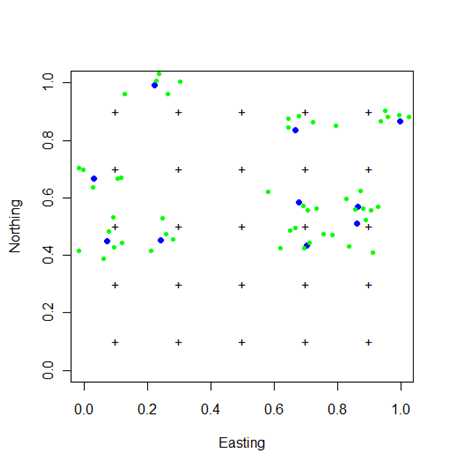
\includegraphics[height=3in]{Ch1/figs/northingeasting}
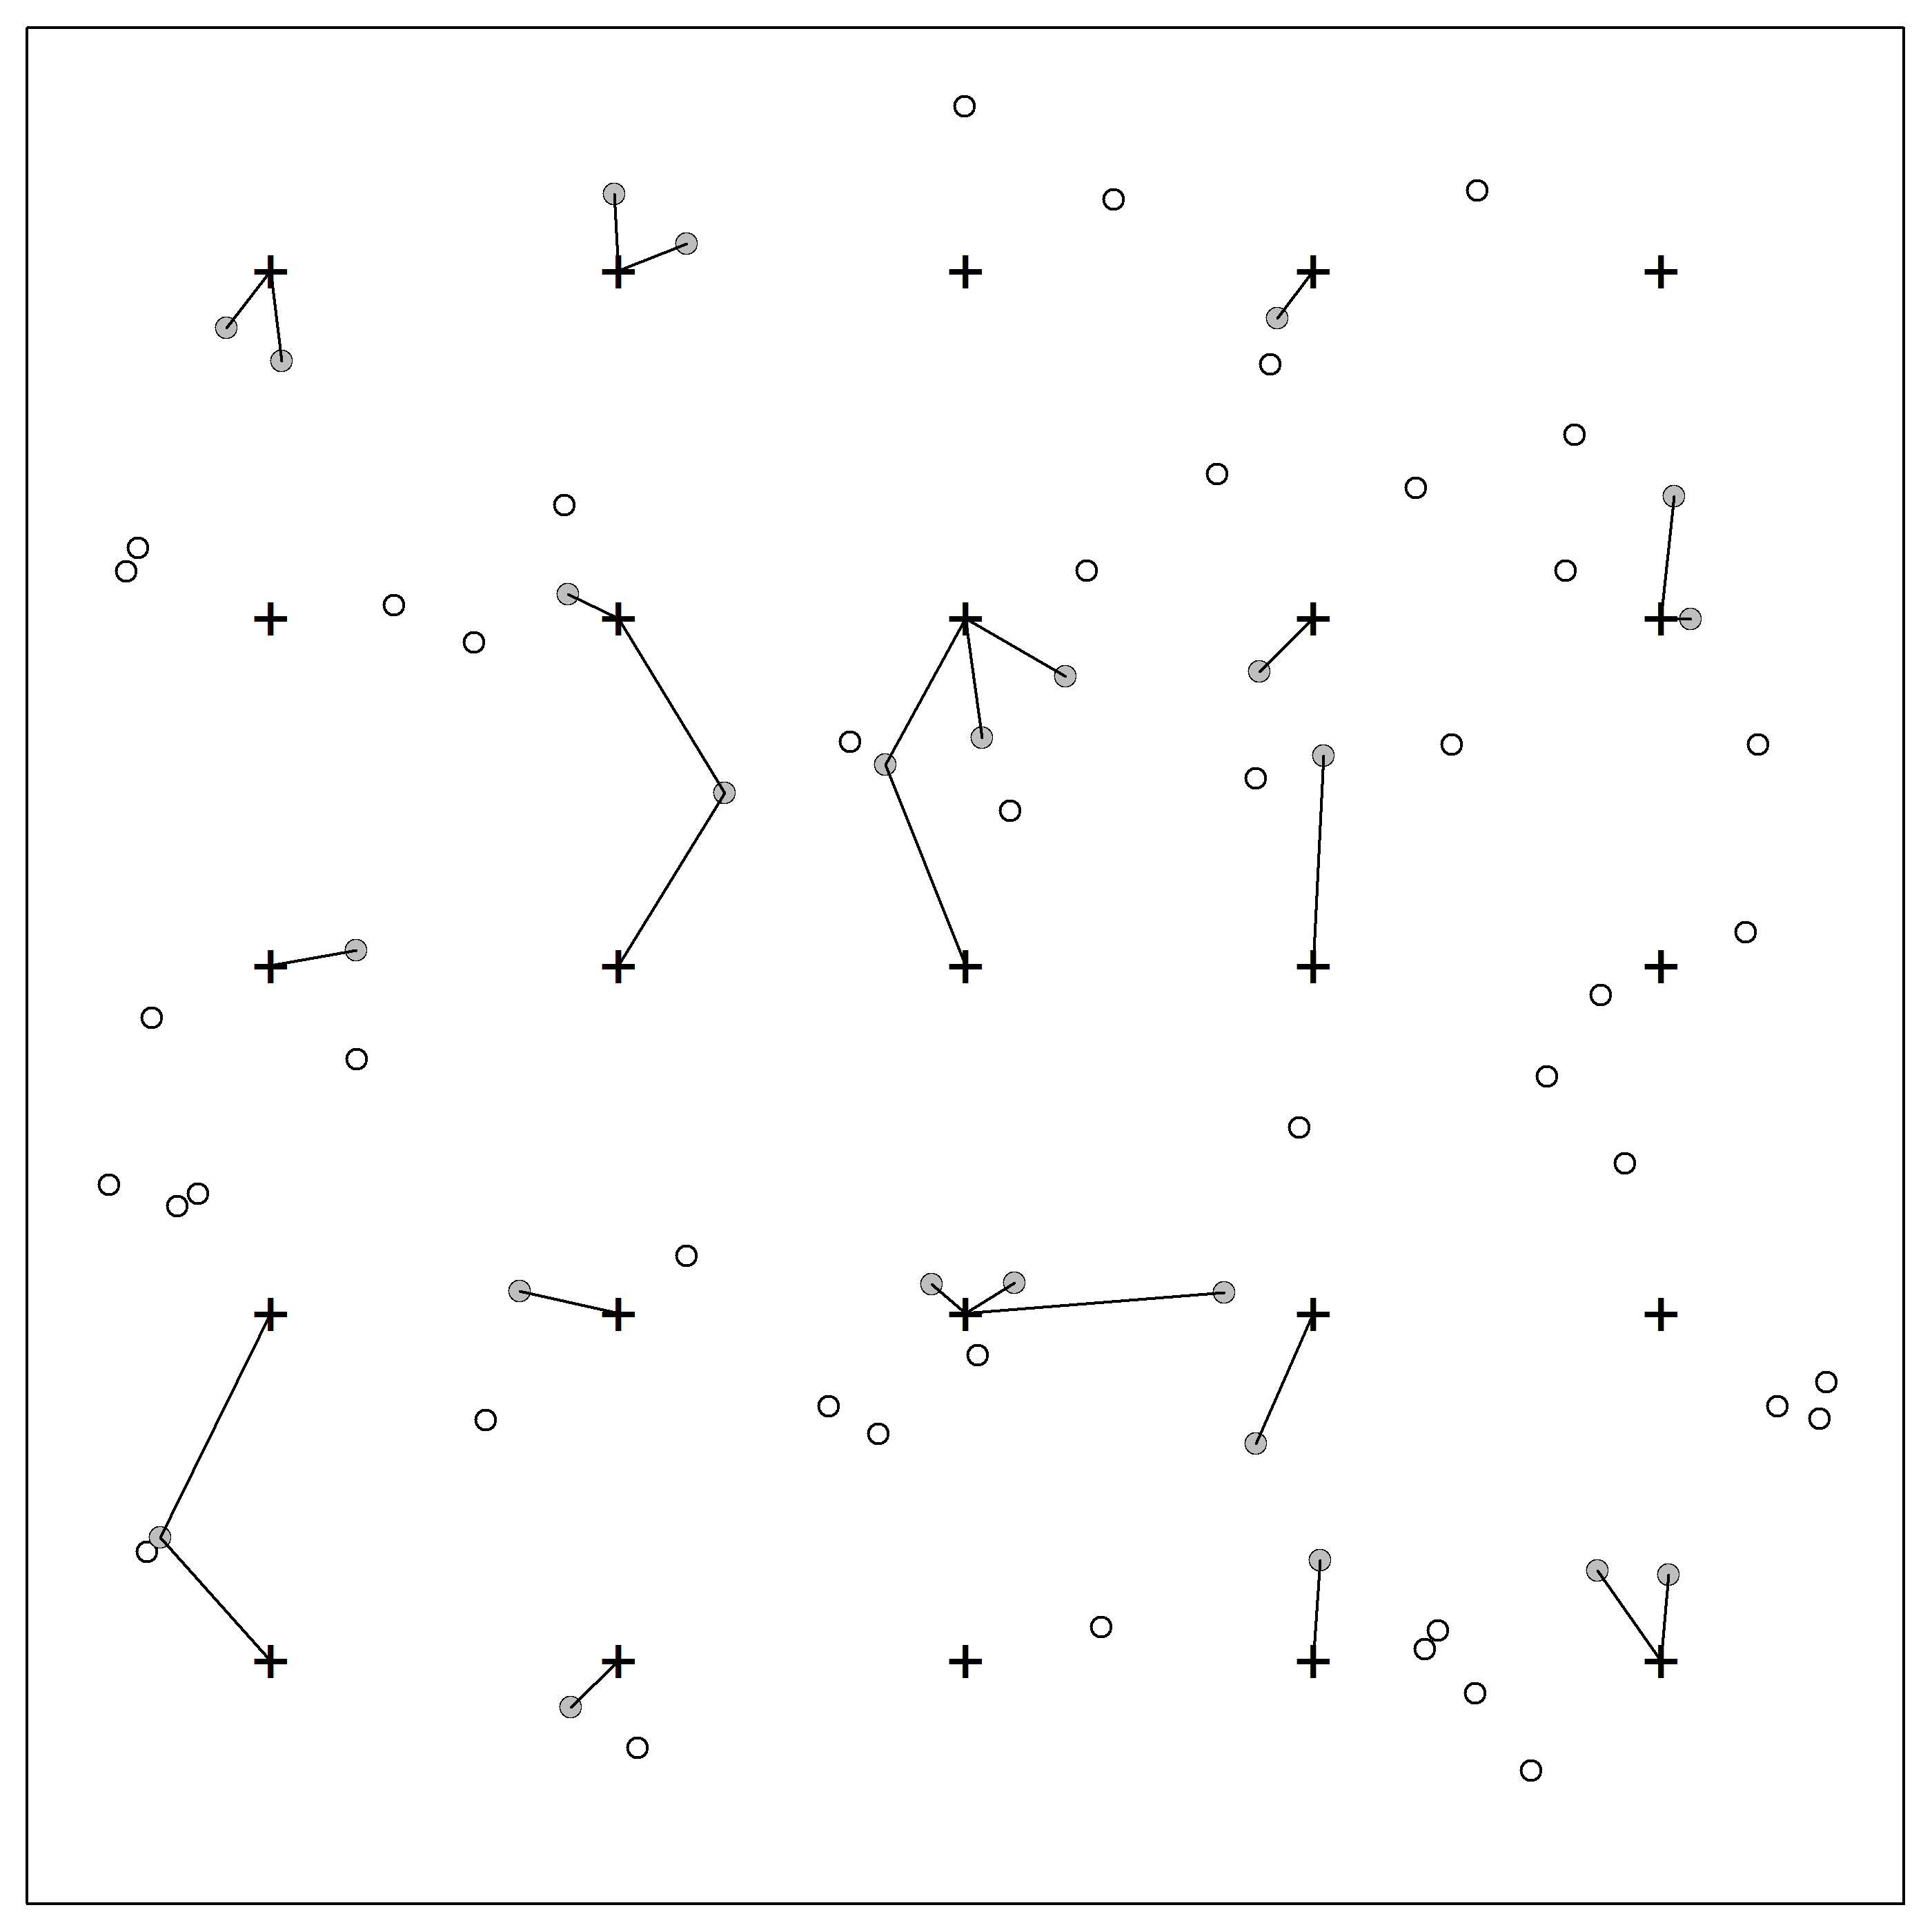
\includegraphics[width=0.5\textwidth]{Ch2/figs/SCR0}
\end{center}
\caption{Population of $N=69$ home-range centers ($\bf s$,
  circles) and 25 trap locations ($\bf x$, crosses). Lines connect
  activity centers to the traps where the individuals were
  detected. As in many SCR models, movement outcomes ($\bf u$)
  are ignored.}
\label{modeling.fig.fig1}
\end{figure}

\subsection{Variations on the SCR theme}

Having now briefly explained each of the model components in
Eq.~\ref{modeling.eq.nyus}, and having
shown how a subset of these components results in a basic SCR model,
we can now discuss other relevant arrangements.
%Although the full model including $u$ and $s$ fully describes the
%ecological process, in practice we usually work with reduced forms of
%this model.
Examples include:
(1) Classical distance sampling \citep{buckland_etal:2001, borchers_etal:2002},
(2) Spatial capture-recapture models with fixed arrays of traps
    \citep{efford:2004, borchers_efford:2008, royle_etal:2009ecol,
           royle_etal:2009jae,
           gardner_etal:2010ecol,royle_etal:2011jwm}, and
(3) Search-encounter models \citep{royle_young:2008,
  royle_etal:2011mee}. %, and
%(4) Capture-recapture distance-sampling \citep{borchers_etal:1998}.
%The constituent pieces of these models are listed in
%Table~\ref{modeling.tab.fam}.
We will now elaborate on some of these distinctions.
%of such models are:
% \begin{enumerate}
%   \item Classical distance sampling \citep{buckland_etal:2001, borchers_etal:2002}
%   \item Spatial capture-recapture models with fixed arrays of traps
%     \citep{efford:2004, borchers_efford:2008, royle_etal:2009ecol,
%            royle_etal:2009jae, gardner_etal:2010ecol,royle_etal:2011jwm}
%   \item Search-encounter models \citep{royle_young:2008, royle_etal:2011mee}.
%   \item Capture-recapture distance-sampling \citep{borchers_etal:1998}.
% \end{enumerate}
% In some classes of models, components for ${\bf u}$ and ${\bf s}$ will be confounded.
% e.g., if ${\bf s}$ are uniform in space and ${\bf u}$ is
% a random draw from some distribution centered at ${\bf s}$, then we might as
% well define ${\bf u}^{*}=\Pr({\bf u})=\int_{s} [{\bf u}|{\bf s}][{\bf
%   s}]ds$ which will itself be uniform
% for reasonable choices of $[{\bf u}|{\bf s}]$.  Some examples
% of typical spatial capture-recapture models and how
% these various model components are manifest in specific cases is
% described as follows:
\begin{enumerate}
\item {\bf Distance sampling}. The last 2 stages of the hierarchy
  are confounded (implicitly) and so analysis is based on the model
  $[y|{\bf u}*] [{\bf u}*]$. The ``process model'' is that of ``uniformity'': ${\bf u}^{*}
  \sim \text{Uniform}({\cal S})$.
%  Sometimes it is argued that distance sampling
%  estimators are ``pooling robust'' which is a way of saying they are
%  (or may be)
%  relatively insensitive to this assumption. That may be true, but the
%  construction of distance sampling estimators makes explicit the
%  uniformity assumption as a mathematical fact.

\item {\bf Spatial capture-recapture model with a fixed array of traps}.
SCR models appear to have little in common with distance sampling
because observations are made only at a pre-defined set of discrete
locations---where traps are placed. However, the models are closely
related in terms of our hierarchical representation above
%\footnote{Really
%they're kind of like point-count distance sampling where the identity
%of individuals is preserved across point samples , and distance is a
%latent variable. i.e., SCR-DS. I feel like this point should be
%emphasized somehow. Here? Later?}.
In SCR models based on fixed arrays, we cannot estimate both
$\Pr(y=1|{\bf u})$ and $\Pr({\bf u}|{\bf s})$---the probability that
an individual ``moves to ${\bf u}$'' cannot be separated from the
probability that it is detected given that it moves to ${\bf u}$,
because of the fact that the observation locations are fixed by
design.
Formally, such SCR models confound $[y|{\bf u}]$  with $[{\bf
  u}|{\bf s}]$ so that the observation model arises as:
\[
 [y|{\bf s}] = \int_{\bf u} [y|{\bf u}][{\bf u}|{\bf s}] \mathrm{d}{\bf u}
\]
This confounding happens because SCR sampling is spatially
biased---restricted to a fixed pre-determined set of locations.
Conversely,
distance sampling confounds $[{\bf u}|{\bf s}][{\bf s}]$ because, essentially, there is
only a single realization of the encounter process.
It is probably
reasonable to assume that $\Pr(y=1|{\bf u})=1$ or at least it is locally
constant for most devices (e.g., cameras, etc..), and thus the
detection model will have the interpretation in terms of movement (see
Chapt. \ref{chapt.rsf} and \ref{chapt.ecoldist}).

\item {\bf Search-encounter models}. What we call
  ``search-encounter'' models \citep{royle_young:2008,royle_etal:2011mee}
  are kind of a hybrid model combining features of SCR models and
  features of distance sampling. Like distance sampling they allow for
  encounters in continuous space which provide direct observations
  from $[{\bf u}|{\bf s}]$. Thus, the
  hierarchical model is fully identified.

  \begin{comment}
  \item {\bf Capture-recapture/distance-sampling}. See
    \citet{borchers_etal:1998}. As with the search-encounter models
    the full hierarchical model is identified: $[y|{\bf u}][{\bf
      u}|{\bf s}][{\bf s}]$ but the quantities don't really mean the
    same thing as before.

    To understand this, we expand the model to accommodate imperfect
    measurements of ${\bf u}$. Let ${\bf u}_{obs}$ be an observation
    of ${\bf u}$ (i.e., made with error). A larger hierarchical model
    is this:
    \[ [y|{\bf u}][{\bf u}_{obs}|{\bf u}][{\bf u}|{\bf s}][{\bf s}]
    \]
    If we make replicate ``instantaneous'' observations of location,
    then information is provided about $[{\bf u}_{obs}|{\bf u}]$
    (i.e., measurement error). However, in a normal distance sampling
    application, with instantaneous sampling, we don't learn anything
    about $[{\bf u}|{\bf s}]$, in effect, we are again confounding
    $[{\bf u}|{\bf s}]$ and $[{\bf s}]$: ${\bf u}^{*} = \int_{s} [{\bf
      u}|{\bf s}][{\bf s}] ds$. So the CR-DS model focuses on:
    \[ [y|{\bf u}^{*}][{\bf u}_{obs}|{\bf u}^{*}][{\bf u}^{*}].
    \]
    Structurally, this is the same basic model as the search-encounter
    model notwithstanding (1) that it is usually talked about in terms
    of repeated measures of distance instead of location and (2) the
    2nd component of the hierarchy is not movement (an ecological
    process) but rather ``measurement error'' and (3) the third
    component is not a home range center but rather a movement outcome
    (``instantaneous location'').  Thus, while the models are
    structurally identically, the meaning and interpretation of
    quantities are distinct.
  \end{comment}

\end{enumerate}


\begin{comment}
\begin{table}
  \centering
  \caption{Spatial capture-recapture models and allies.}
  \begin{tabular}{lll}
    \hline
    Description & Notation & Chapters \\
    \hline
    Full Monte            & $[n(y)|y][y|{\bf u}][{\bf u}|{\bf s}][{\bf s}]$ & --- \\
%    Distance sampling SCR hybrid & $[y|{\bf u}][{\bf u}|{\bf s}][{\bf s}]$ & --- \\
    Standard SCR         & $[y|{\bf s}][{\bf s}]$ & \ref{chapt.scr0} \\
    Distance sampling    & $[y|{\bf u}][{\bf u}]$ & --- \\
    Search-encounter SCR & $[y|{\bf u}][{\bf u}|{\bf s}]$ & \ref{chapt.search} \\
%    Mark-resight SCR     & $[n(y)|y][y|{\bf s}][{\bf s}]$ & \ref{chapt.scr-unmarked,chapt.partialID} \\
    \hline
  \end{tabular}
  \label{modeling.tab.fam}
\end{table}
\end{comment}


%These are
%mostly all semantic and conceptual distinctions which are easy to
%define in a convenient table:
%\begin{table}[ht]
%\centering
%\title{What things mean in each model.}
%\begin{tabular}{c|cc}
%           &   Search encounter models     &  CR-DS  \\  \hline
%  $\sigma$    &  movement       &   measurement error  \\
% ${\bf s}$ & activity center & instaneous location \\
%\end{tabular}
%\end{table}


\begin{comment}

\section{Analysis of spatial capture-recapture models}

\subsection{Models don't have political views!}

Whereas hierarchical modeling is a conceptual framework for
formulating models, the method of inference is independent of model
formulation. Hierarchical models can be analyzed by Bayesian and
non-Bayesian methods. A model is not Bayesian or frequentist -- what
you do to that model is Bayesian or frequentist!
\[
\bullet \mbox{"Hierarchical model"} \ne  \mbox{"Bayesian"}!!!
\]
Thus, analysis of hierarchical models is easily achieved using either
Bayesian or classical (likelihood, frequentist) methods. By
``analysis'' we mean any type of estimation, characterization of
uncertainty, prediction, model selection, or evaluation and we are not
dogmatic about our choice of inference methods. That said, we do
recognize a benefit of the Bayesian approach which is that it
emphasizes model construction and not the construction of
procedures. The Nobel prize\footnote{called something else besides
  Nobel, officially} winning econometrician Christopher Sims (Slides
from the Hotelling Lecture 6/29/2007 at Duke University - cite his
webpage) said it this way: ``Bayesian inference is a way of thinking,
not a basket of 'Methods''' Conversely, ecologistis that are subjected
to a classical statistical curriculum often have only a vague sense of
what the model is that any particular procedure is employing.  We
agree with \citet{little:2006}
that there should be more emphasis on understanding statistical
modeling, and less emphasis on statistical methods.  Toss the ``basket
of methods'' out the window and learn how to model!


We rely strictly on principles and procedures of {\it parametric
  inference} in our analysis of hierarchical models in general and,
specifically, of spatial capture-recapture models. Parametric
inference is that in which we make explicit probability assumptions
about how the data were generated. Inference procedures are then
developed under the assumption that the model is truth, because formal
parametric inference procedures that we understand the joint
probability distribution of everything that is a realization of a
random variable. {\bf There is something missing in the previous sentence. require, maybe?}There are two popular flavors of parametric
inference: {\bf Classical inference}: The joint probability distribution
of observations is the {\bf likelihood}. We maximize it to obtain MLEs
and do other fun things to it. We evaluate procedures by thinking
about what would happen over replicate realizations of data to which
our procedures are applied.  {\bf Bayesian inference} is based on the
posterior distribution, which is the joint probability distribution of
the data and also parameters and possibly other quantities including
latent variables or random effects.

Because SCR models contain a collection of latent variables - random
effects -- a natural framework for classical analysis of the models is
based on integrated likelihood \citep{laird_ware:1982,berger_etal:1999}. That is, while
the observation model is conceptualized conditional on the random
effects (the locations of individuals), classical inference is
formally based on the likelihood constructed from the {\it marginal}
probability distribution of the observations (i.e., {\it
  unconditional} on the random effect). The random effects are removed
from the conditional likelihood by integration (which is accomplished
numerically in spatial capture-recapture models). This approach to
inference has been formalized in the context of SCR models by
\citet{borchers_efford:2008, efford:2011}, and implemented for some
classes of models in the software package {\bf DENSITY} \citep{efford:2004}
and the {\bf R} package \mbox{\tt secr} \citep{efford:2011}.

Bayesian analysis is another natural framework for the analysis of
models containing latent variables or random effects.  Under this
approach, analysis of the model is based on Monte Carlo simulation
from the posterior distribution, which is the product of the
conditional likelihood, the distribution of the random effects, and
perhaps other distributions.  This approach was developed by
\citet{royle_young:2008}, and was motivated by work focused on
modeling individual effects in capture-recapture models. In
particular, a convenient reparameterization of individual covariate
models can be obtained using a method known as data augmentation
\citep{royle_etal:2007}, see \citet{royle:2008} for an application to
classical individual covariate models in \citet{royle:2008}. The close
similarity between individual covariate models and spatial
capture-recapture models, with the individual's activity center ${\bf
  s}$ being the individual covariate, led to the application of the
data augmentation method described by \citet{royle_young:2008} and subsequent papers.

These two technical formulations (classical inference based on
integrated likelihood and Bayesian inference) both provide rigorous solutions to
the inference problems posed by spatial capture-recapture data.  There
are also minor distinctions to be aware of. For example,
as a technical matter, \citet{borchers_efford:2008} and related work, assume
a Poisson point process that is unconditional on $N$ whereas Royle and
Young (2008) and related work assume a binomial point process model
which is conditional on $N$.
%More importantly, Borchers and Efford
%develop the analysis in a way that is unconditional on the point
%process (which is removed from the conditional likelihood by
%integration).  Conversely, the analysis of \citet{royle_young:2008} is
%conditional on the underlying point process. As a technical matter,
%Bayesian analysis allows us to analyze the model that is conditional
%on the underlying point process and will otherwise have more
%flexibility - open populations, using telemetry data, etc.. as will be
%demonstrated in later chapters.

We tend to favor Bayesian inference for conceptual and philosophical
reasons but we also think that  integrated likelihood
for complex point process models may prove difficult. On the other
hand, we suspect that Bayesian
analysis by MCMC
of the model that is conditional on the underlying point process will
prove to be more versatile and generalizable for complex point process
models. We say this only
tentatively and throughout this book we are not exclusive in our views
of inference and use Bayesian and classical methods of inference
interchangeable and opportunistically in this book.
We don't want to get too much into the technical foundations of
Bayesian analysis because there are many good books now including
\citet{link_barker:2010}.  \citet{kery:2010, mccarthy:2007,
  king_etal:2009} and probably others by the time this book is
finished. That said,  Bayesian analysis is introduced at a
level required to get through this book in Chapter 2.


\section{Criticisms of Hierarchical Models}

\hl{If we keep this, remove all SCR references b/c Andy will address
  those in Chapt 5}

We have frequently used the terms
``assumptions'' and ``priors'', which make some people feel
uneasy. Our view is that expressed eloquently by Link (ADD
QUOTE). Furthermore, we note that hierarchical models allow us to
modify any assumption deemed too
restrictive. That is, we can always generalize our models given enough
data. Chapter is a classic example because it addresses
perhaps the most common criticism of SCR, that ``real animals'' don't
have symmetric home ranges. In fact people have written entire papers
beating up on SCR because they \emph{assume} that this the bivariate
normal model for the encounter processes is a rigid requirement of SCR
methods. Although we believe this assumption is quite reasonable in
many contexts, Chapter \ref{chapt.ecoldist} clearly illustrates that
alternatives exist, and that SCR provides a rigorous framework for
testing for departures from this assumption, and even evaluating
hypotheses that may explain why animals move the way they do.


\end{comment}





\section{Summary and Outlook}


Spatial capture-recapture models are hierarchical models, and hierarchical
models are models of multiple random variables that are conditionally
related. It is therefore important that the basic rules of
modeling random variables are understood, and we hope that this chapter
has made some of the basic concepts accessible to ecologists with
rudimentary background in statistics. If some of this material still
seems difficult to grasp, we recommend working with the
provided \R~code, which is perhaps the best way of making the
equations more tangible.

In some respects, it is possible
to understand the jist of SCR without knowing anything about marginal
and conditional relationships. One can always fit models using canned
software and interpret the output without understanding the guts of
the model or the details of the estimation process. For some applied
ecologists, this may be perfectly fine, and this book is meant to be
useful for both statistical novices and ecologists with more advanced
quantitative skills. In most chapters, we begin with a basic conceptual
discussion, then we explain
the technical details that require an understanding of the concepts in
this chapter, and finally we end with one or more worked examples. For
those not interested in the technical details, we recommend focusing
on the chapter introductions and the examples. However, taking the
time to understand the concepts presented in this chapter can only
increase one's ability to tackle the unique and complex problems that
often present themselves when modeling spatial and temporal aspects of
population dynamics.



\chapter{
 GLMs and Bayesian Analysis
}
\markboth{Bayesian Analysis of GLMMs}{}
\label{chapt.glms}

\vspace{.3in}

%%%% STUFF TO DO
%%% 1. Prior lack of invariance to transformation stuff: Reference and Figure
%%% 4. reference for sampling from f() with bounded support
%%% 6. Check Bayesian p-value definition
%%% 8. spell check this document

%%% NEW STUFF TO DO
%%% add bugs model for BBS Poisson regression?
% XXX Should DIC/selection/FIT material go into Chapter 8? XXXXXXX

%%% some ref chapters need filling in; eg section 3.8; section 3.8.2
%%% Once Ch2 is ready, ask Richard to go over the sections on Poisson and Binommial GL(M)Ms to make sure there isn't too much redundancy between Ch2 and 3
%XXXX I commented out those sections that we agreed should be moved to Ch2, some stuff on Bayesian p value calculation

A major theme of this book is that spatial capture-recapture models
are, for the most part, just generalized linear models (GLMs) wherein
the covariate, distance between trap and home range center, is
partially or fully unobserved  -- and therefore regarded as
a random effect. Outside of capture-recapture, such models
are usually referred to as generalized linear mixed models (GLMMs)
and, therefore, SCR models can be thought of as a specialized type of
GLMM. Naturally then, we should consider analysis of these slightly
simpler models in order to gain some experience and, hopefully,
develop a better understanding of spatial capture-recapture models.

In this chapter, we consider classes of GL(M)Ms -- Poisson and
binomial (i.e., logistic regression) models -- that will prove to be
enormously useful in the analysis of capture-recapture models of all
kinds. Many readers are likely familiar with these models already because
they are among
the most useful models in ecology and, as
such, have received considerable attention in many introductory and
advanced texts. We focus on them here in order to introduce the
readers to the analysis of such models in {\bf R} and {\bf WinBUGS} or
{\bf JAGS},
which we will
translate directly to the analysis of SCR models in subsequent
chapters.

Bayesian analysis is convenient for analyzing GL(M)Ms because it allows
us to work directly with the conditional model -- i.e., the model that
is conditional on the random effects, using computational methods
known as Markov chain Monte Carlo (MCMC). Learning how to do Bayesian
analysis of GLMs and GLMMs using the {\bf BUGS} language is, in part, the purpose
of this chapter. We focus here on the use of {\bf WinBUGS} because it
is the most popular ``{\bf BUGS} engine''. However, later in the book
we transition to another popular {\bf BUGS} engine known as {\bf
  JAGS} \citep{plummer:2009} which stands for {\it Just Another Gibbs
  Sampler}. For most of our purposes, the specification of models in
either platform is the same, but {\bf JAGS} is under active
development at the present time while {\bf WinBUGS} no longer is,
having transitioned to 
{\bf OpenBUGS} \citep{lunn_etal:2009} which is still in active
development.  
 While we use {\bf BUGS} of one sort or another to do the Bayesian
computations, we organize and summarize our data and execute {\bf
  WinBUGS} or {\bf JAGS} from within {\bf R} using the packages 
\mbox{\tt
  R2WinBUGS} \citep{sturtz_etal:2005}, \mbox{\tt R2jags} \citep{su_yajima:2011} or \mbox{\tt rjags} \citep{plummer:2009}.  \citet{kery:2010}, and
\citet{kery_schaub:2011} provide excellent and accessible introductions to the basics
of Bayesian analysis and GL(M)Ms using {\bf WinBUGS}.
We don't want to
be too redundant with those books and so we avoid a detailed
treatment of Bayesian methodology and software usage - instead just providing a cursory
overview so that we can move on and attack the problems we're most
interested in related to spatial capture-recapture.  In addition,
there are a number of texts that provide general introductions to
Bayesian analysis, MCMC, and their applications in ecology including
\citet{mccarthy:2007}, \citet{kery:2010}, \citet{link_barker:2010}, and
\citet{king_etal:2008}.


While this chapter is about Bayesian analysis of GL(M)Ms, such models
are routinely analyzed using likelihood methods too.
Later in
this book (Chapt. \ref{chapt.mle}), we will use likelihood methods to analyze SCR models but,
for now, we concentrate on providing a basic introduction to Bayesian
analysis because that is the approach we will use in a majority of
cases in later chapters.

%Richard will move this section to previous chapter
% \section{ Notation}

% We will sometimes use conventional ``bracket notation'' \index{bracket
%   notation} to refer to
% probability distributions. If $y$ is a random variable then $[y]$
% indicates its distribution or its probability density/mass function
% (pdf, pmf) depending on context. If $x$ is another random variable
% then $[y|x]$ is the conditional distribution of $y$ given $x$, and
% $[y,x]$ is the joint distribution of $y$ and $x$. To differentiate
% specific distributions in some contexts we might label them $g(y)$,
% $g(y|\theta)$, $f(x)$, or similar. We will also write $y \sim
% \mbox{Normal}(\mu,\sigma^{2})$ to indicate that $y$ ``is distributed as'' a normal
% random variable with parameters $\mu$ and $\sigma^{2}$. The expected value
% or mean of a random variable is $E[y] = \mu$ ,and $Var[y] = \sigma^{2}$ is
% the variance of $y$.   To indicate specific observations we'll use an
% index such as ``$i$''. So, $y_{i}$ for $i=1,2,\ldots,n$ indicates
% observations for $n$ individuals. Finally, we write $\Pr(y)$ to indicate specific probabilities, i.e., of events ``$y$'' or similar.


% To illustrate these concepts and notation, suppose $z$ is a binary
% outcome (e.g., species occurrence) and we might assume the model: $z
% \sim \mbox{Bern}(p)$ for observations.  Under this model $\Pr(z=1) =
% \psi$, which is also the expected value $E[z] = \psi$. The variance is
% $Var[z] = \psi*(1-\psi)$ and the probability mass function (pmf) is $[z]
% = \psi^{z} (1-\psi)^{1-z}$. Sometimes we write $[z|\psi]$ when it is
% important to emphasize the conditional dependence of $z$ on $\psi$. As
% another example, suppose $y$ is a random variable denoting whether or
% not a species is detected if an occupied site is surveyed. In this
% case it might be natural to express the pmf of the observations $y$
% {\it conditional} on $z$. That is, $[y|z]$. In this case, $[y|z=1]$ is
% the conditional pmf of $y$ given that a site is occupied, and it is
% natural to assume that $[y|z=1] = \mbox{Bern}(p)$ where $p$ is the
% ``detection probability'' - the probability that we detect the
% species, given that it is present. The model for the observations $y$
% is completely specified once we describe the other conditional pmf
% $[y|z=0]$. For this conditional distribution it is sometimes
% reasonable to assume $\Pr(y=1|z=0) = 0$ (\citet{mackenzie_etal:2002};
% see also \citet{royle_link:2006}). That is, if the species is absent,
% the probability of detection is 0. This implies that
% $\Pr(y=0|z=0)=1$. To allow for situations in which the true state $z$
% is unobserved, we  assume that $[z]$ is Bernoulli with parameter
% $\psi$.  In this case, the marginal distribution of $y$ is
% \[
%  [y] = [y|z=1]Pr(z=1) + [y|z=0]Pr(z=0)
% \]
% because $[y|z=0]$ is a point mass at $y=0$, by assumption, the marginal
% probability that $y=1$ is
% \[
% \Pr(y=1) = p \psi
% \]
% and the marginal probability that $y=0$ is
% \[
% \Pr(y=0) = (1-p)*\psi + (1-\psi)
% \]
%END of section Richard will move to previous chapter

\section{
GLMs and GLMMs}
\label{glms.sec.glmms}
We have asserted already that SCR models work out most of the time to
be variations of GL(M)Ms. You might therefore ask: What
are these GLM and GLMM models, anyhow?   These models are covered extensively in
many very good applied statistics books and we refer the reader
elsewhere for a detailed introduction.  The
classical references for GLMs are \citet{nelder_wedderburn:1972} and
 \citet{mccullagh_nelder:1989}. In addition, we think \citet{kery:2010},
\citet{kery_schaub:2011}, and \citet{zuur_etal:2009} are all
accessible treatments.
Here, we'll give the 1
minute
treatment of GL(M)Ms, not trying to be complete but rather only
to preserve a coherent organization to the book.


The GLM is an extension of standard linear
models allowing the response
variable to have some distribution from the exponential family of
distributions. This includes the normal
distribution but also others such as the Poisson, binomial,
gamma, exponential, and many more. In addition, GLMs allow the
response variable to be related to the predictor variables (i.e.,
covariates) using a link function, which is usually nonlinear.  
%Finally, GLMs typically
% accommodate a relationship between the mean and variance.
% The GLM consists of three components:
% \begin{itemize}
% \item[1.] A probability distribution for the dependent variable $y$,
% from the exponential family of probability distributions.
%\item[2.] A ``linear predictor'' $\eta = {\bf x}'{\bm \beta}$  .
% \item[2.] A ``linear predictor'' $\eta = \beta_0 + x \beta_1$, where $x$ is the predictor variable.
% \item[3.] A link function $g$ that relates $E[y]$ to the linear predictor, $E[y] = \mu = g^{-1}(\eta)$. Therefore $g(E[y]) = \eta$.
% \end{itemize}
% XXXX ISNT THIS REDUNDANT? XXXXXXXXX
% The dependent variable $y$ is assumed to be an outcome from a
% distribution of the exponential family. The mean of the distribution of $y$ is assumed to depend on predictor variables $x$ according to
% \[
%  %g(E[y]) = {\bf x}'{\bm \beta}
%  g(E[y]) =\beta_0 + x \beta_1
% \]
% where $E[y]$ is the expected value of $y$, and ${\bf x}'{\bm \beta}$
% is termed the {\it linear predictor}, i.e., a linear function of the
% predictor variables ${\bf x}$ with unknown parameters ${\bm \beta}$ to be
% estimated.  
% The function $g$ is the link function. In standard GLMs,
% the variance of $y$ is a function $V$ of the mean of $y$: $Var(y) =
% V(\mu)$ (see below for examples).
% XXXXXXXXXXXXXXXXXXXXXXXXXXXXXXXXXXXXX SEEMS REDUNDANT UP TO HERE XXXXXXXXXXXXXXXX
The GLM consists of three components:
\begin{itemize}
\item[1.] A probability distribution for the dependent (or response) variable $y$,
from the exponential family of probability distributions.
\item[2.] A ``linear predictor'' $\eta = \beta_0 + x \beta_1$, where
  $x$ is a predictor variable (i.e., a covariate).
\item[3.] A link function $g$ that relates the expected value of $y$, $\mathbb{E}(y)$, to the linear predictor, $\mathbb{E}(y) = \mu = g^{-1}(\eta)$. Therefore $g(\mathbb{E}(y)) = \eta = \beta_0 + x \beta_1$ .
\end{itemize}
A key aspect of GLMs is that 
$g(\mathbb{E}(y))$ is assumed to be a linear function of the
predictor variable(s), here $x$, with unknown parameters, here $\beta_0$ and $\beta_1$, to be
estimated. In standard GLMs,
the variance of $y$ is a function $V$ of the mean of $y$: $\mbox{Var}(y) =
V(\mu)$ (see below for examples).
As an example, a Poisson GLM posits that $y \sim \mbox{Poisson}(\lambda)$ with $\mathbb{E}(y)
=\lambda$ and usually the model for the mean is specified using the
{\it log link function} by
\[
\log(\lambda_{i}) = \beta_0 + \beta_{1}  x_{i}
\]
The variance function is $\mbox{V}(y_{i}) = \lambda_{i}$.  
To see how a Poisson GLM works, use the {\bf R} code below to simulate
some data and then estimate the parameters:
{\small
\begin{verbatim}
> set.seed(13)
> n <- 100            # set sample size
> beta0 <- -2         # set intercept term
> beta1 <- 1.5        # set coefficient
> x <- rnorm(n, 0,1)  # generate a predictor variable, x

> linpred <- beta0 + beta1*x  # calculate linear predictor of E(y)
> y <- rpois(n, exp(linpred))   # generate observations from model
\end{verbatim} }
The {\bf R} function {\tt glm()} fits a GLM to the data we just
generated and returns estimates of $\beta_0$ and $\beta_1$, which we
see are fairly close to the data generating values above:
\begin{alltt}
> glm(y \(\sim\) 1 + x, family='poisson')      # the fit model
\end{alltt}
This produces the output:
\begin{alltt}
Call:  glm(formula = y \(\sim\) 1 + x, family = "poisson")

Coefficients:
(Intercept)            x  
     -2.007        1.446  

[... some output deleted ...]
\end{alltt}
In this summary output, the maximum likelihood estimates (MLEs) of the
regression parameters  $\beta_0$ and $\beta_1$ are labeled ``\mbox{\tt
  Coefficients}.'' We see that these are not too different from the
data-generating values (-2 and 1.5, respectively). 


The
binomial GLM posits that $y_{i} \sim \mbox{Binomial}(K,p)$ where $K$
is the fixed sample size parameter and $\mathbb{E}(y_{i}) = K \times p_{i}$. Usually
the model for the mean is specified using the {\it logit link
  function} according to
\[
 \text {logit}(p_{i}) = \beta_{0} + \beta_{1}  x_{i}
\]
Where $\text {logit}(p) = \text {log}(p/(1-p))$.  The inverse-logit function,
consequently, is $\text {logit}^{-1}(p) =
\text {exp}(p)/(1+\text {exp}(p))$.

A GLMM is the extension of GLMs to accommodate ``random
effects''. Often this involves adding a normal random effect to the
linear predictor. One simple example is using a random intercept,  ${\bm \alpha}$:
\[
 \log(\lambda_{i}) = \alpha_{i} + \beta_{1} x_{i}
\]
where
\[
 \alpha_{i} \sim \mbox{Normal}(\mu,\sigma^{2})
\]
Many other probability distributions and formulations of the linear
predictor might be considered.  GLMMs are enormously useful in
ecological modeling applications for modeling variation due to 
subjects, observers, spatial
or temporal stratification, clustering, and dependence that arises
from any kind of group structure and, of course, because SCR models
prove to be a type of GLM with a random effect, but one that does not
enter the mean linearly. 

%It is not widely appreicated that
%the link function and
%distribution of the random effect interact directly to affect the
%implied probability distribution of the linear predictor. For the
%Poisson case just considered, $\lambda_{i}$ has a log-normal
%distribution. However, if we set $\lambda_{i} = \alpha_{i}exp(\beta*x_{i})$
%where $\alpha_{i}$ has a Gamma distribution, then $\lambda_{i}$ has
%similarly a gamma distribution with modified scale parameter.  These
%different model assumptions are seldom evaluated formally in practice
%although in many practical situations (in ecology), they imply
%specific things about the ecological process being studied
%(e.g., see \citet{royle_dorazio:2008} section XYZ on occupancy
%logit/cloglog etc..).



\section{Bayesian Analysis}

Bayesian analysis is less familiar to many ecological researchers because
they are often educated only in the classical
statistical paradigm of frequentist inference. But advances in
technology and increasing exposure to the benefits of Bayesian analysis
are fast making Bayesians out of people or at least making Bayesian
analysis an acceptable, general alternative to classical, frequentist
inference.

Conceptually, the main thing about Bayesian inference is that it uses
probability directly to characterize uncertainty about things we don't
know.  ``Things'', in this case, are parameters of models and, just as
it is natural to characterize uncertain outcomes of stochastic
processes using probability, it seems natural also to characterize
information about unknown parameters using probability. At least
this seems natural to us and, we think, most ecologists either
explicitly adopt that view or tend to fall into that point of view
naturally.  Conversely, frequentists use probability in many different
ways, but never to characterize uncertainty about
parameters\footnote{To hear this will be shocking to some readers
  perhaps.}. Instead, frequentists use probability to characterize the
behavior of {\it procedures} such as estimators or confidence
intervals (see below). It is surprising that people readily
adopt a philosophy of statistical inference in which the things you
don't know (i.e., parameters) should {\it not} be regarded as random
variables, so that, as a consequence, one cannot use probability to
characterize one's state of knowledge about them.


\subsection{Bayes' Rule}

As its name suggests, Bayesian analysis makes use of Bayes' rule in
order to make direct probability statements about model
parameters. Given two random variables $z$ and $y$, Bayes' rule relates
the two conditional probability distributions $[z|y]$ and $[y|z]$ by
the relationship:
\begin{equation}
[z|y] = [y|z][z]/[y].
\label{glms.eq.bayes}
\end{equation}
Bayes' rule itself is a mathematical fact and there is no debate in
the statistical community as to its validity and relevance to many
problems. Generally speaking, these distributions are characterized as
follows: $[y|z]$ is the conditional probability distribution of $y$
{\it given} $z$, $[z]$ is the marginal distribution of $z$ and $[y]$
is the marginal distribution of $y$. In the context of Bayesian
inference we usually associate specific meanings in which $[y|z]$ is
thought of as ``the likelihood'', $[z]$ as the ``prior'' and so on. We
leave this for later because here the focus is on this expression of
Bayes' rule as a basic fact of probability.

As an example of a simple application of Bayes' rule,
consider the problem of determining species presence at a sample
location based on imperfect survey information. Let $z$ be a binary
random variable that denotes species presence $(z=1)$ or absence
$(z=0)$, let $\Pr(z=1) = \psi$ where $\psi$ is usually called
occurrence probability, ``occupancy'' \citep{mackenzie_etal:2002} or ``prevalence''.
Let $y$ be the {\it observed} presence
($y=1$) or absence ($y=0$) (or, strictly speaking, detection and non-detection), and let $p$ be the probability that a
species is detected in a single survey at a site given that it is
present. Thus, $\Pr(y=1|z=1)=p$. The interpretation of this is that,
if the species is present, we will only observe it with
probability $p$. In addition, we assume here that $\Pr(y=1|z=0) =
0$. That is, the species cannot be detected if it is not present which
is a conventional view adopted in most biological sampling problems (but
see \citet{royle_link:2006}).
If we survey a site $K$ times but never detect the species,
then this clearly does not imply that the species is not present
($z=0$) at this site but that we failed to observe it. 
Rather, our degree of belief in $z=0$ should be
made with a probabilistic statement, namely the conditional probability
$\Pr(z=1|y_1=0,\ldots,y_{K}=0)$. If the $K$ surveys are independent so
that we might regard $y_{k}$ as $iid$ Bernoulli trials, then the total
number of detections, say $y$, is Binomial with probability $p$, and
we can use Bayes' rule to compute the probability that the species is present
given that it is not detected in $K$ samples, i.e., $\Pr(z=1|y_{1} =
0, \ldots, y_{K} = 0)$. In words, the expression
we seek is:
\[
\Pr(\mbox{present} | \mbox{not detected}) = \frac{\Pr(\mbox{not detected} |
  \mbox{present})\Pr(\mbox{present})}{\Pr(\mbox{not detected})}
\]
Mathematically, this is
\begin{eqnarray*}
\Pr(z=1|y=0) &= &\frac{\Pr(y=0|z=1)\Pr(z=1)}{\Pr(y=0) } \\
             &= & \frac{(1-p)^{K} \psi}{ (1-p)^K \psi + (1-\psi) }.
\end{eqnarray*}
The denominator here, 
the probability of not detecting the species, 
is composed of two parts: (1) not observing the species given that it
is present (this occurs with probability $(1-p)^{K} \psi$) and (2) the
species is not present (this occurs with probability $1-\psi$).
To apply this result,
suppose that $K=2$ surveys are done at a wetland for a species of
frog, and the species is not detected there. Suppose further that $\psi
= 0.8$ and $p = 0.5$ are obtained from a prior study.  Then the
probability that the species is present at this site, even though it
was not detected, is
$(1-0.5)^2 \times 0.8/((1-0.5)^2 \times 0.8 + (1-0.8)) = 0.5$. 
That is, there is a
50/50 chance that the site is occupied despite the fact that the
species wasn't observed there.

In summary, Bayes' rule provides a simple linkage between the
conditional probabilities $[y|z]$ and $[z|y]$, which is useful whenever
we need to deduce one from the other.

\subsection{Principles of Bayesian Inference}

Bayes' rule as a basic fact of probability is not disputed.
What is controversial to some is the scope and manner in which Bayes'
rule is applied by Bayesian analysts. Bayesian analysts assert that
Bayes' rule is relevant, in general, to all statistical problems by
regarding all unknown quantities of a model as realizations of random
variables -- this includes data, latent variables, and also
parameters. Classical (non-Bayesian) analysts sometimes object to
regarding parameters as outcomes of random variables. Classically,
parameters are thought of as ``fixed but unknown'' (using the
terminology of classical statistics).
Indeed, a common misunderstanding on the distinction between Bayesian and
frequentist inference goes something like this ``in frequentist
inference parameters are fixed but unknown but in a Bayesian analysis
parameters are random.'' At best this is a sad caricature of the
distinction and at worst it is downright wrong. 
In Bayesian analysis the
parameters are also unknown and, in fact, there is a single data-generating
value of each parameter, and so they are also fixed.
The difference is that the fixed
but unknown values are  regarded as having been generated from some
probability distribution. Specification of that probability
distribution is necessary to carry out Bayesian analysis, but it is not
required in classical frequentist inference.


To see the general relevance of Bayes' rule in the context of
statistical inference, let $y$ denote observations - i.e., data -
and let $[y|\theta]$ be the observation model (often colloquially
referred to as the ``likelihood'').  Suppose $\theta$ 
is a parameter of
interest having (prior) probability distribution $[\theta]$ (also simply referred to as the prior). These are
combined to obtain the posterior distribution using Bayes' rule, which
is:
\[
 [\theta|y]= [y|\theta][\theta]/[y]
\]
Asserting the general relevance of Bayes' rule to all statistical
problems, we can conclude that the two main features of Bayesian
inference are that: (1) parameters, $\theta$, are regarded as realizations of
a random variable and, as a result, (2) inference is based on the
probability distribution of the parameters given the data,
$[\theta|y]$,
which is
called the posterior distribution. This is the result of using Bayes'
rule to combine the ``likelihood'' and the prior distribution.  The
key concept is regarding parameters as realizations of a random
variable because, once you admit this conceptual view, this leads
directly to the posterior distribution, a very natural quantity upon
which to base inference about things we don't know -  including
parameters of statistical models.  In particular, $[\theta|y]$ is a
probability distribution for $\theta$ and therefore we can make direct
probability statements to characterize uncertainty about
$\theta$.

The denominator of our invocation of Bayes' rule, $[y]$,
is the marginal distribution of the data $y$.  We note without further
remark right now that, in many practical problems, this can be an
enormous pain to compute. The main reason that the Bayesian paradigm
has become so popular in the last 20 years or so is because methods
have been developed
for characterizing the posterior distribution that do not
require that we possess a mathematical understanding of $[y]$. This means
we never have to compute it or know what it looks like, or know
anything specific about it.

%A Bayesian
%assumes, just like a frequentist, that there was a single
%data-generating value of that parameter - a fixed, and unknown value
%that produced the given data set.
%The distinction between Bayesian and frequentist approaches is that
%Bayesians regard the parameter as a random variable, and its value as
%the outcome of a random variable, on par with the observations. 


While we can understand the conceptual basis of Bayesian inference
merely by understanding Bayes' rule -- that's really all there is to it
-- it is not so easy to understand the basis of classical
frequentist inference. 
% which is mostly like
% \footnote{as characterized by Christopher A. Sims, winner of the 
% Sveriges Riksbank Prize in Economic Sciences in Memory of Alfred Nobel
% in his
% Hotelling Lecture 6/29/2007 at Duke University - 
% \url{http://sims.princeton.edu/yftp/EmetSoc607/AppliedBayes.pdf}:
% ``Bayesian inference is a way of thinking,
% not a basket of 'Methods'''} a ``basket of
% methods'' with little coherent organization. 
What is mostly coherent
in frequentist inference is the manner in which procedures are evaluated -- the performance of a given procedure is
evaluated by ``averaging over'' hypothetical realizations of $y$,
regarding the {\it estimator} as a random variable. For example, if
$\hat{\theta}$ is an estimator of $\theta$ then the frequentist is
interested in $\mathbb{E}_{y}(\hat{\theta}|y)$ which is used to characterize
bias. If the expected value of $\hat{\theta}$, when averaged over
realizations of $y$, is equal to $\theta$, then $\hat{\theta}$ is
unbiased.

The view of parameters as being random variables 
allows Bayesians to use probability to make direct probability
statements about parameters. Frequentist inference procedures do not
permit direct probability statements to be made about parameter
values.
Instead, 
the view of parameters as fixed constants and estimators as random variables
leads to interpretations that are not so straightforward. For
example confidence intervals having the interpretation ``95\%
probability that the interval contains the true value'' and p-values
being ``the probability of observing an outcome of the test statistic as extreme or more than
the one observed.'' These are far from intuitive interpretations to
most people.  Moreover, this is conceptually problematic to some
because we will never get to observe the hypothetical realizations that characterize the
performance of our procedure.

While we do tend to favor Bayesian inference for the conceptual
simplicity (parameters are random, posterior inference), we mostly
advocate for a pragmatic non-partisan approach to inference because,
frankly, some of the frequentist methods are actually very
convenient in certain situations, and will generally yield very
similar inferences about parameters, as we will see in later chapters.


\subsection{Prior distributions}
%add paper richard mentioned in the meeting...

The prior distribution $[\theta]$ is an important feature of Bayesian
inference. As a conceptual matter,
the prior distribution characterizes ``prior beliefs'' or ``prior
information'' about a parameter. Indeed,
an oft-touted benefit of Bayesian analysis is the ease with which
prior information can be included in an analysis. 
However, more commonly, the prior is chosen to
express a lack of prior information, even if previous studies have
been done and even if the investigator does in fact know quite a bit
about a parameter.
This is because
the manner in which prior information is embodied in a prior (and the
amount of information) is
usually very subjective and thus the result can wind up being very
contentious; e.g., different investigators might report different
results based on subjective assessments of prior information. Thus it is usually
better to ``let the data speak'' and use priors that reflect absence
of information beyond the data set being analyzed. An example for an
uninformative prior is a $\mbox{Uniform}(0,1)$ for a probability, or a
\mbox{Uniform}(-$\infty$, $\infty$) (also called a ``flat'' or
``improper'' prior) for an unbounded continuous
parameter. Alternatively, people use ``diffuse priors''; these contain
some information, but (ideally) not enough to exert meaningful
influence on the posterior. An example for a diffuse prior could be a normal distribution with a large standard deviation.

But still the need occasionally arises to embody prior information or
beliefs about a parameter formally into the estimation scheme.
 In SCR models we often have a parameter that is closely linked
to ``home range size'' and thus auxiliary information on the home
range size of a species can be used as prior information, which may improve parameter estimation (e.g., see
\citet{chandler_royle:2012}; also Chapt. \ref{chapt.scr-unmarked}).

At times the situation arises where a prior can inadvertently impose
substantial effect on the posterior of a parameter, and that is not desirable.
For example, we use data augmentation
to deal with the fact that the population size $N$ is an unknown parameter
 \citep{royle_etal:2007} which is equivalent to imposing a $\mbox{Binomial}(M,\psi)$
 prior on $N$ for some integer $M$ (see Sec. \ref{closed.sec.da}). One has to take care to make sure
 that $M$ is sufficiently large so as to not affect the posterior
 distribution on $N$ (see Fig. \ref{mcmc.fig.timeseries2}, and also
 \citet[][Ch. 5]{kery_schaub:2011}).
Another situation that we have
 to be careful of is that
prior 
distributions are {\it not} invariant to transformation of the
parameter,
and therefore neither are posterior distributions
\citep[][Sec. 6.2.1]{link_barker:2010}. Thus, a prior that is ostensibly
non-informative on one scale, may be very informative on another
scale. 
For example, if we have a flat prior on $\mbox{logit}(p)$ for some probability
parameter $p$, this is very different from having a 
$\mbox{Uniform}(0,1)$ prior 
on $p$. We show an example where this makes a difference in
Chapt. \ref{chapt.scr0}. Nonetheless, it is always possible to assess
the influence of prior choice, and it is often the case (with
sufficient data and a structurally identifiable model) that the
influence of priors is negligible. 

\subsection{Posterior Inference}

In Bayesian inference, we are not focusing on estimating a single
point or interval but rather on characterizing a whole distribution --
the posterior distribution -- from which one can report any summary of
interest. A point estimate might be the posterior mean, median, mode,
etc..  In many applications in this book, we will compute 95\%
Bayesian confidence intervals using the 2.5\% and 97.5\% quantiles of the
posterior distribution. For such intervals, it is correct to say
$\Pr(L < \theta < U) = 0.95$. That is, ``the probability that $\theta$
lies between $L$ and $U$ is $0.95$". 

As an
example, suppose we conducted a Bayesian analysis to estimate
detection probability ($p$) of some species at a study site, and we
obtained a posterior distribution of beta(20,10) for the parameter
$p$. The following {\bf R} commands demonstrate how we make inferences based
upon summaries of the posterior distribution:
\begin{verbatim}
> post.median <- qbeta(0.5, 20, 10)
[1] 0.6704151
> post.95ci <- qbeta(c(0.025, 0.975), 20, 10)
[1] 0.4916766 0.8206164
\end{verbatim}
Thus, we can state that there is a 95\% probability that $\theta$ lies
between 0.49 and 0.82. Fig. \ref{densityvsdetection.fig} shows the
posterior along with the summary statistics.
It is not a subtle thing that such statements 
cannot be made using frequentist methods, although people tend to say
it anyway and not really understand why it is wrong or even that it is
wrong. 
%This is  because
%frequentists have not been successful in convincing people to
%over-ride their natural inclination on how to use probability.  As a
%frequentist, you simply cannot use probability in the manner that you
%would like to.

\begin{figure}
\begin{center}
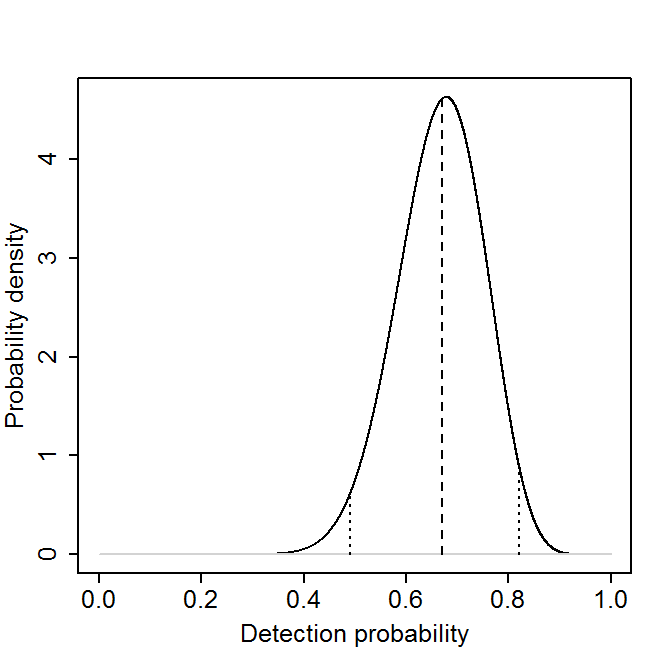
\includegraphics[height=2.5in]{Ch3-Bayes/figs/densityvsdetection}
%get figure file from Ch7 folder
\end{center}
\caption{Probability density plot of a hypothetical
 posterior distribution of beta(20,10); dashed lines 
 indicate mean and upper and lower 95\% interval}
\label{densityvsdetection.fig}
\end{figure}

%%XXX Andy - I think this paragraph is a bit harsh
%% can we tone it down just a pinch?



% As a conceptual matter, Bayesian inference based on the posterior
% allows us 
%  to make an inference conditional on the data that we
% actually observed, i.e., what we actually know.  To us, this seems
% logical - to condition on what we know. Conversely, frequentist
% inference is based on considering average performance over
% hypothetical unobserved data sets (i.e., the ``relative frequency''
% interpretation of probability).  Frequentists know that their
% procedures work well when averaged over all hypothetical, unobserved,
% data sets but no one ever really knows how well they work for the
% specific data set analyzed. That seems like a relevant question to
% biologists who oftentimes only have their one, extremely valuable,
% data set. 
\begin{comment}
 This distinction comes into play a lot in exposing
philosophical biases in the peer review of statistical analyses in
ecology in the sense that, despite these opposing conceptual views to
inference (i.e., conditional on the data you have, or averaged over
hypothetical realizations), those who conduct a Bayesian analysis are
often (in ecology, almost always) required to provide a frequentist
evaluation of their Bayesian procedure.
\end{comment}


\subsection{Small sample inference}

The posterior distribution is an exhaustive summary of the
state-of-knowledge about an unknown quantity. It is {\it the}
posterior distribution - not an estimate of that thing. It is also
not, usually, an approximation except to within Monte Carlo error (in
cases where we use simulation to calculate it, see
Sec. \ref{glms.sec.convergence}).  One of the great virtues of
Bayesian analysis which is not widely appreciated is that posterior
inference is not ``asymptotic'', which is to say, valid in a limiting
sense as the sample size tends to infinity. Rather, posterior
inference is valid for {\it any} sample size and, in particular, {\it
  the} sample size on-hand.  Conversely, almost all frequentist
procedures are based on asymptotic approximations to the procedure
which is being employed.

There seems to be a prevailing view in statistical ecology that
classical likelihood-based procedures are virtuous because of the
availability of simple formulas and procedures for carrying out
inference, such as calculating standard errors, doing model selection
by Akaike information criterion (AIC), and assessing goodness-of-fit.  In large samples, this may be
an important practical benefit, but the theoretical validity of these
procedures cannot be asserted in most situations involving small
samples.  This is not a minor issue because it is typical in many
wildlife sampling problems -- especially in surveys of carnivores or
rare/endangered species -- to wind up with a small, sometimes extremely
small, data set, that is nevertheless extremely valuable
\citep{foster_harmsen:2012}. For examples: A recent paper
 \citep{hawkins_racey:2005}
 on the fossa
(\emph{Cryptoprocta ferox}), estimated
an adult density of 0.18 adults per sq. km based on a sample size of 20 animals captured
over 3 years. 
\citet{sepulveda_etal:2007}
 estimated density of the 
endangered southern river otter (\emph{Lontra provocax})
based on 12 individuals captured over 3
years,  
 \citet{gardner_etal:2010ecol} estimated 
density from a study of the Pampas cat (\emph {Leopardus colocolo}), a species for which very little
is known, based on only 22 captured individuals over 
a two year study period,   \citet{trolle_kery:2005} reported only 9 individual
ocelots captured and \citet{jackson_etal:2006} captured 6 individual
snow leopards (\emph{Panthera uncia}) using camera trapping. 
Thus, almost all likelihood-based
analysis of data on rare and/or
secretive carnivores necessarily and flagrantly violate one of Le
Cam's Basic Principles: ``If you need to use asymptotic
arguments, do not forget to let your number of observations tend to
infinity'' \citep{lecam:1990}.

The biologist thus faces a dilemma with such data. On one hand, these
data sets, and the resulting inference, are often criticized as being
poor and unreliable. Or, even worse\footnote{Actual quote from a
  referee}, ``the data set is so small, this is a poor analysis.''  On
the other hand, such data may be all that is available for species
that are extraordinarily important for conservation and management.
The Bayesian framework for inference provides a valid, rigorous, and
flexible framework that is theoretically justifiable in arbitrary
sample sizes. This is not to say that one will obtain precise
estimates of density or other parameters, just that your inference is
coherent and justifiable from a conceptual and technical statistical
point of view. That is, for example when we estimate the density $D$ of some animal population, we report the posterior probability
$\Pr(D|data)$ which is easily interpretable and just what it is
advertised to be and we don't need to do a simulation study to
evaluate how well the reported $\Pr(D|data)$ deviates from the
``true'' $\Pr(D|data)$ because they are the same quantity.

\begin{comment}
% note this is a distinction between SCR and CR not Bayes and non-BAyes
SCR better than ordinary CR 
for analysis of all
CR data sets because they more efficiently use the available information 
that is inherent in almost all capture-recapture studies.
\end{comment}


\section{Characterizing posterior distributions by MCMC simulation}

In practice, it is not really feasible to ever compute the marginal
probability distribution $[y]$, the denominator resulting from
application of Bayes' rule
(Eq. \ref{glms.eq.bayes}). For decades (even centuries!) this impeded the adoption of
Bayesian methods by practitioners. Or, the few Bayesian analyses done
were based on asymptotic normal approximations to the posterior
distribution. While this was useful from a theoretical and
technical standpoint and, practically, it allowed people to make the
probability statements that they naturally would like to make, it was
kind of a bad joke around the Bayesian water-cooler to, on one hand,
criticize classical statistics for being, essentially, completely ad
hoc in their approach to things but then, on the other hand, have to
devise various approximations to what they were trying to
characterize. The advent of Markov chain Monte Carlo (MCMC) methods
has made it easier to calculate posterior distributions for just about
any problem to sufficient levels of precision.

Broadly speaking, MCMC is a class of methods for drawing random
samples
(i.e., simulating from or just ``sampling'') from the target posterior
distribution.  Thus, even though we might not recognize the posterior
as a named distribution or be able to analyze its features
analytically, e.g., devise mathematical expressions for the mean and
variance, we can use these MCMC methods to obtain a large sample from
the posterior and then use that sample to characterize features of the
posterior. What we do with the sample depends on our intentions --
typically we obtain the mean or median for use as a point estimate,
and take a confidence interval based on Monte Carlo estimates of the
quantiles. 
\begin{comment}
% tried to make point here about difference between approximations
% but failed
 These are estimates, but not like frequentist
estimates. Rather, they are Monte Carlo estimates with an associated
Monte Carlo error which is largely determined arbitrarily by the
analyst. They are not estimates qualified by a sampling distribution
as in classical statistics. If we run our MCMC long enough then our
reported value of $\mathbb{E}(\theta|y)$ or any feature of the posterior
distribution is precisely what we say it is. There is no ``sampling
variation'' in the frequentist sense of the word.  In summary, the
MCMC samples provide a Monte Carlo characterization of {\it the}
posterior distribution.
\end{comment}


\subsection{What Goes on Under the MCMC Hood}

We will develop and apply MCMC methods in some detail for spatial
capture-recapture models in Chapt. \ref{chapt.mcmc}. Here we provide
a simple illustration of some basic ideas related to the practice of MCMC.

A type of MCMC method relevant to most problems is Gibbs sampling 
\citep{geman_geman:1984} which we address in more detail in Chapt. \ref{chapt.mcmc}.
Gibbs sampling 
involves 
iterative simulation from the ``full
conditional''
distributions (also called conditional posterior
distributions). The full conditional distribution for an unknown
quantity is the conditional distribution of that quantity given every
other random variable in the model - the data and all other
parameters (see Sec. \ref{glms.sec.rules} for rules of how to construct full conditionals).
For example, for a normal regression model
\footnote{We center the 
independent variable here so that things look more familiar in the result} with $y \sim
\mbox{Normal}(\beta_0 + \beta_1 (x-\bar{x}) , \sigma^{2})$
where lets say $\sigma^{2}$ is known, the full conditionals are, using
 ``bracket notation'',
\[
[\beta_0|y,\beta_1]
\]
 and
\[
[\beta_1|y,\beta_0].
\]
We might use our knowledge of probability to identify these
mathematically. In particular, by Bayes' Rule, $[\beta_0|y,\beta_1] =
[y|\beta_0,\beta_1][\beta_0|\beta_1]/[y|\beta_1]$ and similarly for
$[\beta_1|y,\beta_0]$. For example, if we have priors for 
$[\beta_0] = \mbox{Normal}(\mu_{\beta_0}, \sigma^{2}_{\beta_0})$ 
and 
$[\beta_1] = \mbox{Normal}(\mu_{\beta_1}, \sigma^{2}_{\beta_1})$ then
some algebra reveals that 
\begin{equation}
[\beta_0|y,\beta_1] = \mbox{Normal}\left(w \bar{y} + (1-w)\mu_{\beta_0},
(\tau n + \tau_{\beta_0})^{-1} \right)
\label{glms.eq.alpha}
\end{equation}
where $\tau = 1/\sigma^{2}$ and $\tau_{\beta_0} = 1/\sigma^{2}_{\beta_0}$
(the inverse of the variance is sometimes called {\it precision}), and
$w = \tau n/(\tau n + \tau_{\beta_0})$. We see in this case that the
posterior mean is a {\it precision-weighted} sum of the sample mean
$\bar{y}$ and the prior mean $\mu_{\beta_0}$, and the posterior {\it precision} 
is the sum of the precision of the likelihood and that of the
prior. These results are typical of many
classes of problems. In particular, note that as the prior precision
tends to 0, i.e., $\tau_{\beta_0} \rightarrow 0$, then the posterior of
$\beta_0$ tends to  $\mbox{Normal}(\bar{y}, \sigma^{2}/n)$. We recognize the 
variance of this distribution as that of the variance of the sampling
distribution of $\bar{y}$ and its mean is in fact the MLE of $\beta_0$
for this model. 
The conditional posterior of $\beta_1$ has a very similar form:
\begin{equation}
 [\beta_1|y,\beta_0]  = \mbox{Normal}\left(
\frac{ \tau (\sum_{i} y_{i}(x_{i}-\bar{x}) ) + \tau_{\beta_1} \mu_{\beta_1}}
{ \tau \sum_{i} (x_{i}-\bar{x})^{2} + \tau_{\beta_1}},
(\tau \sum_{i} (x_{i}-\bar{x})^{2} + \tau_{\beta_1} )^{-2} \right)
\label{glms.eq.beta}
\end{equation}
which might look slightly unfamiliar, but note that if $\tau_{\beta_1} = 0$, 
then the mean of this distribution is the familiar $\hat{\beta_1}$, and
the variance is, in fact, the sampling variance of $\hat{\beta_1}$. 
\begin{comment}Andy, you use a slightly different representation of the full conditionals then I do in Ch7; might be good to reconcile, or maybe I can just point out in Ch7 that I'm using a slightly different representation so that people don't get confused. Let me know what you'd prefer.\end{comment}
The MCMC algorithm for this model has us simulate in succession,
repeatedly, from those two distributions. See \citet{gelman_etal:2004}
for more examples of Gibbs sampling for the normal model, and we also
provide another example in Chapt. \ref{chapt.mcmc}. A
conceptual representation of the MCMC algorithm for this simple model
is therefore:

\vspace{.1in}

\parbox[h]{6in}{
{\tt Algorithm}: Gibbs Sampling for linear regression

\vspace{.1in}

\hspace{.25in}
     {\tt  0. Initialize} $\beta_0$ {\tt and} $\beta_1$

\vspace{.1in}


\hspace{.25in}
     {\tt  Repeat} $\{$

\vspace{.1in}
   
\hspace{.45in}
        {\tt 1. Draw a new value of} $\beta_0$ {\tt from Eq.} \ref{glms.eq.alpha}

\vspace{.1in}

\hspace{.45in}
        {\tt 2. Draw a new value of} $\beta_1$  {\tt from Eq.} \ref{glms.eq.beta}

\vspace{.1in}

\hspace{.25in}
     $\}$
}

\vspace{.1in}

As we just saw for this simple ``normal-normal'' model, it is sometimes
possible to specify the full conditional distributions
analytically. In general, when certain so-called conjugate prior
distributions are used, which have an analytic form that, in a
statistical
sense, ``matches'' the likelihood, then the form of the full conditional distributions
is also similar to that of the observation model. In this normal-normal
case, the normal distribution for the mean parameters is the conjugate
prior for the normal observation model, and thus the full-conditional
distributions are also normal. This is convenient because, in such
cases, we can simulate directly from them using standard methods (or
{\bf R}
functions).  But, in practice, we don't really ever need to know such
things because most of the time we can get by using a simple
algorithm, called the Metropolis-Hastings (henceforth ``MH'')
algorithm, to obtain samples from these full conditional distributions
without having to recognize them as specific, named, distributions.
This gives us enormous freedom in developing models
and analyzing them without having to resolve them mathematically
because to implement the MH algorithm we need only identify the full
conditional distribution up to a constant of proportionality, that
being the marginal distribution in the denominator (e.g., $[y|\beta_1]$
above).

We will talk about the Metropolis-Hastings algorithm shortly, and we
will use it extensively in the analysis of SCR models (e.g., Chapt.
\ref{chapt.mcmc}).

\subsection{Rules for constructing full conditional distributions}
\label{glms.sec.rules}

The basic strategy for constructing full-conditional distributions for
devising MCMC algorithms can be reduced conceptually to a couple of
basic steps summarized as follows:

\begin{description}
\item[   (step 1)] Identify all stochastic components of the model and
  collect their probability distributions;
\item[   (step 2)] Express the full conditional in question
  as proportional to the product of all probability distributions
  identified in step 1;
\item[   (step 3)] Remove the ones that don't have the focal parameter in them.
\item[   (step 4)] Do some algebra on the result in order to identify
  the resulting probability distribution function (pdf) or mass
  function (pmf).
\end{description}

% {\flushleft (step 1)} Collect all stochastic components of the model;
% {\flushleft (step 2)} Recognize and express the full conditional in question
%   as proportional to the product of all components;
% {\flushleft (step 3)} Remove the ones that don't have the focal parameter in them.
% {\flushleft (step 4)} Do some algebra on the result in order to identify the resulting pdf or pmf.

Of the 4 steps, the last of those is the main step that requires quite
a bit of statistical experience and intuition because various
algebraic tricks can be used to reshape the mess into something
recognizable -- i.e., a standard, named distribution. But step 4 is not
necessary if we decide instead to use the Metropolis-Hastings algorithm
as described below.

In the context of our simple linear regression model that we've been 
working with, to characterize $[\beta_0|y,\beta_1]$ we first apply step 1
and identify the model components as: $[y|\beta_0, \beta_1]$, with
prior distributions $[\beta_0]$
and $[\beta_1]$. Step 2 has us write $[\beta_0|y,\beta_1] \propto
[y|\beta_0,\beta_1][\beta_0][\beta_1]$.  Step 3: We note that $[\beta_1]$ is not a
function of $\beta_0$ and therefore we remove it to obtain $[\beta_0|y,\beta_1]
\propto [y|\beta_0,\beta_1][\beta_0]$. Similarly, applying step 2 and 3 for $\beta_1$ we obtain $[\beta_1|y,\beta_0]
\propto [y|\beta_0,\beta_1][\beta_1]$. We apply step 4 and manipulate
these algebraically to arrive at the result (which we provided in
Eqs. \ref{glms.eq.alpha} and \ref{glms.eq.beta}) or, alternatively, we can
sample them indirectly using the Metropolis-Hastings algorithm, which we 
discuss now.


\subsection{Metropolis-Hastings algorithm}

The Metropolis-Hastings (MH) algorithm is a completely generic method for
sampling from any distribution, say $[\theta]$. In our applications,
$[\theta]$ will typically be the full conditional distribution of
$\theta$.
While we sometimes use Gibbs sampling, we seldom
use ``pure'' Gibbs sampling because full conditionals do not always take the form of known distributions we can sample from directly. In such cases, we use MH to sample from the full conditional distributions.
When the MH algorithm is used to sample from  full
conditional distributions of a Gibbs sampler the resulting hybrid algorithm is
called
 {\it Metropolis-within-Gibbs}.
In Sec. \ref{GLMM.sect.mcmc} we will
 construct such an algorithm for a simple class of models. We discuss both the Gibbs and the MH algorithm, as well as their hybrid in more depth in Chapt. \ref{chapt.mcmc}.

The MH algorithm generates candidate values for the parameter(s) we want to estimate from some
proposal or candidate-generating distribution that may be conditional
on the current value of the parameter, denoted by
$h(\theta^{*}|\theta^{t-1})$. Here, $\theta^{*}$ is the {\it candidate}
or proposed
value and $\theta^{t-1}$ is the value of $\theta$ at the previous time step, i.e., at iteration $t-1$ of
the MCMC algorithm.  The proposed value
is accepted with probability

\[
r = \frac{ [\theta^{*}] h(\theta^{t-1}|\theta^{*})}
    { [\theta^{t-1}] h(\theta^{*}|\theta^{t-1}) }
\]
which is called the MH acceptance probability.
This ratio can sometimes be $>1$ in which case we set it equal to
1. It is useful to note that $h()$ can be any probability distribution.


In the context of using the MH algorithm to do MCMC (in which case
the target distribution is a full-conditional or posterior distribution), an
important fact is, no matter
the choice of $h()$, we can compute the MH acceptance probability
directly because 
the marginal distribution of $y$ cancels from both the numerator and
denominator of $r$. This is the magic of the MH algorithm.


\section{Bayesian Analysis using the BUGS language}

We won't be too concerned with devising our own MCMC algorithms for
every analysis, although we will do that a few times for fun.  More
often, we will rely on the freely available software package {\bf
  WinBUGS} or {\bf JAGS} for doing this.  We will always execute these
{\bf BUGS} engines from within {\bf R} using the \mbox{\tt R2WinBUGS}
\citep{sturtz_etal:2005} or, for {\bf JAGS}, the \mbox{\tt R2jags}
\citep{su_yajima:2011} or \mbox{\tt rjags} \citep{plummer:2009}
packages.  {\bf WinBUGS} and {\bf JAGS} are MCMC black boxes that take
a pseudo-code description (i.e., written in the {\bf BUGS} language)
of all of the relevant stochastic and deterministic elements of a
model and generate an MCMC algorithm for that model. But you never get
to see the algorithm. Instead, {\bf WinBUGS}/{\bf JAGS} will run the
algorithm and return the Markov chain output - the posterior samples
of model parameters.

The great thing about using the {\bf BUGS} language is that it forces
you to become intimate with your statistical model - you have to write
each element of the model down, admit (explicitly) all of the various
assumptions, understand what the actual probability assumptions are
and how data relate to latent variables and data and latent variables
relate to parameters, and how parameters relate to one another.

While we normally use {\bf WinBUGS}, we note that {\bf OpenBUGS} is
the current active development tree of the {\bf BUGS} project. See
\citet[][]{kery:2010} and \citet[][especially
Appendix 1]{kery_schaub:2011} for more on practical analysis in {\bf
  WinBUGS}.  
Those books should be consulted for a more comprehensive
introduction to using {\bf WinBUGS}.  Recently we have migrated many
of our analyses to {\bf JAGS} \citep{plummer:2009}, which we adopt
later in the book. You can refer to \citet{hobbs:2011} for an
ecological introduction to {\bf JAGS}.  Next, we provide an example of
a Bayesian analysis using {\bf WinBUGS}.

\subsection{Linear Regression in WinBUGS}
\label{GLMM.sect.linear}

We provide a brief introductory example of a normal regression model
using a small simulated data set. The following commands are executed
from within your {\bf R} workspace.
First, simulate a covariate $x$ and observations $y$ having
prescribed intercept, slope and variance:
\begin{verbatim}
 > x <- rnorm(10)
 > mu <- -3.2 + 1.5*x
 > y <- rnorm(10,mu,sd=4)
\end{verbatim}
The {\bf BUGS} model specification for a normal regression model is
written within {\bf R} as a character string input to the command
\mbox{\tt cat()} and
then dumped to a text file named \mbox{\tt normal.txt}:
\begin{alltt}
> cat("
 model\{ 
   for (i in 1:10)\{ 
      y[i] \(\sim\) dnorm(mu[i],tau)         # the likelihood
      mu[i] <- beta0 + beta1*x[i]     # the linear predictor
    \}
   beta0 \(\sim\) dnorm(0,.01)               # prior distributions
   beta1 \(\sim\) dnorm(0,.01)
   sigma \(\sim\) dunif(0,100)
   tau <- 1/(sigma*sigma)             # tau is the precision
\}				       #   and a derived parameter
",file="normal.txt")
\end{alltt}
Alternatively, you
can write the model specifications directly within a text file and
save it in your current working directory, but we do not usually take
that approach in this book.

The {\bf BUGS} dialects\footnote{We use this to mean {\bf WinBUGS},
  {\bf OpenBUGS} and {\bf JAGS}} parameterize the normal distribution
in terms of the mean and inverse-variance, called the precision. Thus,
\mbox{\tt dnorm(0,.01)} implies a variance of 100.  We typically use
diffuse normal priors for mean parameters, $\beta_0$ and $\beta_1$ in
this case, but sometimes we might use uniform priors with suitable
bounds $-B$ and $+B$.  Also, we typically use a $\text{Uniform}(0,B)$
prior on standard deviation parameters \citep{gelman:2006}.  But
sometimes we might use a gamma prior on the precision parameter
$\tau$.  In a {\bf BUGS} model file, every variable referenced in the
model description has to be either data, which will be input (see
below), a random variable which must have a probability distribution
associated with it using the tilde character ``$\sim$'' (a.k.a. ``twiddle'')
or it has to be a derived parameter connected to variables
and data using an assignment arrow: ``\mbox{\tt <-}''.


To fit the model, we need to describe various data objects to {\bf
  WinBUGS}. In particular,
we create an {\bf R} list object called \mbox{\tt data} which
are the data objects identified in the {\bf BUGS} model file.
 In the example, the
data consist of two objects which exist as $y$ and $x$ in the {\bf R}
workspace and also in the {\bf WinBUGS} model definition.
 We also create an {\bf R} function
that produces a list of starting values, \mbox{\tt inits}, that get sent to
{\bf WinBUGS}. In general, starting
values are optional. We recommend to always provide reasonable
starting values where possible, both for structural parameters and
also random effects\footnote{While {\bf WinBUGS} is reasonably robust to a
  wide range of more or less plausible starting values, {\bf JAGS} is
  a lot more sensitive and especially with more complex models you
  might actually have to spend some time thinking about how to specify
  good starting values to get the model running (Appendix 1); we
  will come back to this issue when we use {\bf JAGS}}. 
 Finally, we identify
the names of the parameters (labeled correspondingly in the {\bf WinBUGS}
model specification) that we want {\bf WinBUGS} to save the MCMC output
for. In this example, we will ``monitor'' the parameters
$\beta_0$, $\beta_1$, $\sigma$ and $\tau$.
{\bf WinBUGS} is executed using the {\bf R} command
\mbox{\tt bugs()}.
We set the option \mbox{\tt debug=TRUE} if we want the {\bf WinBUGS}
GUI to stay open (useful for analyzing MCMC output and looking at the
{\bf WinBUGS} error log). Also, we set \mbox{\tt working.dir=getwd()}
so that {\bf WinBUGS} output files and the log file are saved in the
current {\bf R} working directory (note that sometimes you will need to specify the place where you installed {\bf WinBUGS} within the \mbox{\tt bugs()} call, using the \mbox{\tt bugs.directory} argument).
  All of these activities together look like this:
  
 
{\small
\begin{verbatim}
 > library(R2WinBUGS)    # "load" the R2WinBUGS package
 > data <- list( y=y, x=x)
 > inits <- function()
 > list ( beta1=rnorm(1),beta0=rnorm(1),sigma=runif(1,0,2) )
 > parameters <- c("beta0","beta1","sigma","tau")
 > out <- bugs(data, inits, parameters, "normal.txt", n.thin=1, n.chains=2,
             n.burnin=2000, n.iter=6000, debug=TRUE,working.dir=getwd())
\end{verbatim}
}

Note that the previously created objects defining data, initial values
and parameters to monitor are passed to the function \mbox{\tt
  bugs()}.  In addition, various other things are declared: The number
of parallel Markov chains (\mbox{\tt n.chains}), the thinning rate
(\mbox{\tt n.thin}), the number of burn-in iterations (\mbox{\tt
  n.burnin}) and the total number of iterations (\mbox{\tt n.iter}).
To develop a detailed understanding of the various parameters and
settings used for MCMC, consult a basic reference such as
\citet{kery:2010}. We also come back to these issues in the following
section (\ref{GLMM.sec.practical}) and in Chapt. \ref{chapt.mcmc}.
A common question is ``how should my data be formatted?'' That depends
on how you describe the model in the {\bf BUGS} language, and how your
data are input into {\bf R}. There is no unique way to describe any
particular model and so you have some flexibility. We talk about data
format further in the context of capture-recapture models and SCR
models in Chapt. \ref{chapt.scr0} and elsewhere. 


You should execute all of the commands given above and then
close the {\bf WinBUGS} GUI, and the data will be
read back into {\bf R} (or specify \mbox{\tt debug=FALSE} in the 
\mbox{\tt bugs()} call).  We don't
want to give instructions on how to navigate and use the GUI -- but you
can fire up {\bf WinBUGS} and read the help files, or see Chapt. 4 from
\citet{kery:2010} for a brief introduction.
The print command applied to the object \mbox{\tt out} prints some
basic summary output (this is slightly edited):

{\small
\begin{verbatim}
> print(out,digits=2)
Inference for Bugs model at "normal.txt", fit using WinBUGS,
 2 chains, each with 6000 iterations (first 2000 discarded)
 n.sims = 8000 iterations saved
          mean   sd  2.5%   25%   50%   75% 97.5% Rhat n.eff
beta0    -6.62 1.64 -9.77 -7.63 -6.64 -5.63 -3.29    1  4200
beta1     0.81 1.20 -1.63  0.09  0.80  1.54  3.24    1  5100
sigma     4.99 1.56  2.93  3.92  4.66  5.70  8.85    1  8000
tau       0.05 0.03  0.01  0.03  0.05  0.07  0.12    1  8000
deviance 58.72 3.21 55.06 56.35 57.85 60.26 67.15    1  6200

For each parameter, n.eff is a crude measure of effective sample size,
and Rhat is the potential scale reduction factor (at convergence, Rhat=1).

DIC info (using the rule, pD = Dbar-Dhat)
pD = 2.5 and DIC = 61.3
\end{verbatim}
}

% Inference for Bugs model at "normal.txt", fit using WinBUGS,
%  2 chains, each with 6000 iterations (first 2000 discarded), n.thin = 2
%  n.sims = 4000 iterations saved
%           mean   sd  2.5%   25%   50%   75% 97.5% Rhat n.eff
% beta0    -2.43 1.84 -6.21 -3.50 -2.42 -1.34  1.27    1  4000
% beta1     2.62 1.54 -0.42  1.68  2.62  3.57  5.67    1  4000
% sigma     5.29 1.66  3.11  4.14  4.95  6.05  9.39    1  4000
% tau       0.05 0.02  0.01  0.03  0.04  0.06  0.10    1  4000
% deviance 59.85 3.24 56.18 57.47 59.00 61.37 68.32    1   840

% For each parameter, n.eff is a crude measure of effective sample size,
% and Rhat is the potential scale reduction factor (at convergence, Rhat=1).

% DIC info (using the rule, pD = Dbar-Dhat)
% pD = 2.6 and DIC = 62.4

 In the {\bf WinBUGS} output you see a column called ``\mbox{\tt
   Rhat}'', as well as one called ``\mbox{\tt
   n.eff}''. These are convergence diagnostics (the $\hat{R}$ or Brooks-Gelman-Rubin statistic and the effective sample size) and we will discuss those in the following section, \ref{glms.sec.convergence}. DIC is the
deviance information criterion (\citet{spiegelhalter_etal:2002}, see section \ref{glms.sec.modsel})
 which
some people use in a manner similar to AIC although it is recognized
to have some problems in hierarchical models \citep{millar:2009}. We
consider use of DIC in the context of SCR models in Chapt. \ref{chapt.gof}.

%Richard will move and write this section into Ch2
% \subsection{Modeling categorical variable effects with dummy
%   variables}
% \label{glms.sec.dummy}

% Make point here that we often have categorical variables -- with
% nominal levels these are ``factors'', and we model these using dummy
% variables but sometimes in \bugs we use ``index variables''.
%end of section Richard will develop in Ch2



\section{Practical Bayesian Analysis and MCMC}
\label{GLMM.sec.practical}

The mere execution of a Bayesian analysis using the {\bf BUGS} language, as demonstrated with the linear regression example, is fairly straight forward. There are, however, a number of really important practical issues to be
considered in any Bayesian analysis and we cover some of these briefly
here before we move on to implementing slightly more complex GL(M)Ms in a Bayesian framework.

\subsection{Choice of prior distributions}
\label{glms.sec.choice}

Bayesian analysis requires that we choose prior distributions for all
of the structural parameters of the model (we use the term structural
parameter to mean all parameters that aren't customary thought of as
latent variables). We will strive to use priors that are meant to
express little or no prior information - default or customary
``non-informative'' or diffuse priors. This will be
$\mbox{Uniform}(a,b)$ priors for parameters that have a natural
bounded support and, for parameters that live on the real line we use
either (1) diffuse normal priors, as we did in the linear regression example above; (2) improper uniform priors which
have unbounded support, e.g., $[\theta] \propto 1$, or (3) sometimes
even a bounded $\mbox{Uniform}(a,b)$ prior, if that greatly improves
the performance of {\bf WinBUGS} or other software doing the MCMC for
us.  In {\bf WinBUGS} a prior with low precision, $\tau$, where $\tau
= 1/\sigma^2$, such as $\mbox{Normal}(0,.01)$ will typically be
used. Of course $\tau = 0.01$ ($\sigma^{2} = 100$) might be very
informative for a regression parameter depending on its magnitude and
scaling of $x$.  Therefore, we recommend that predictor variables (covariates) {\it
  always} be standardized to have mean 0 and variance 1. 

{\bf Lack of invariance of priors to transformation.} Clearly there
are a lot of choices for ostensibly non-informative priors, and the
degree of non-informativeness depends on the parameterization. For
example, a natural non-informative prior for the intercept of a
logistic regression
\[
\mbox{logit}(p_{i}) = \beta_0 + \beta_1 x_{i}
\]
would be a very diffuse normal prior,
$[\beta_0] = \mbox{Normal}(0,\mbox{Large})$ or even
 $\beta_0 \sim
\mbox{Uniform}(-\mbox{Large},\mbox{Large})$.
However, we might also use a prior on the parameter $p_0
= \mbox{logit}^{-1}(\beta_0)$, which is $\Pr(y=1)$ for the value $x=0$. 
Since $p_0$ is a
probability a natural choice is $p_0 \sim \mbox{Uniform}(0,1)$. 
These priors are very different in their implications. For example, if
we choose the normal prior for $\beta_0$ with variance
$\mbox{Large} = 5^2$ and look at the implied prior for $p_{0}$
we have the result shown in Fig. \ref{glms.fig.impliedprior}
which looks nothing like a $\mbox{Uniform}(0,1)$ prior.
\begin{figure}[ht]
\begin{center}
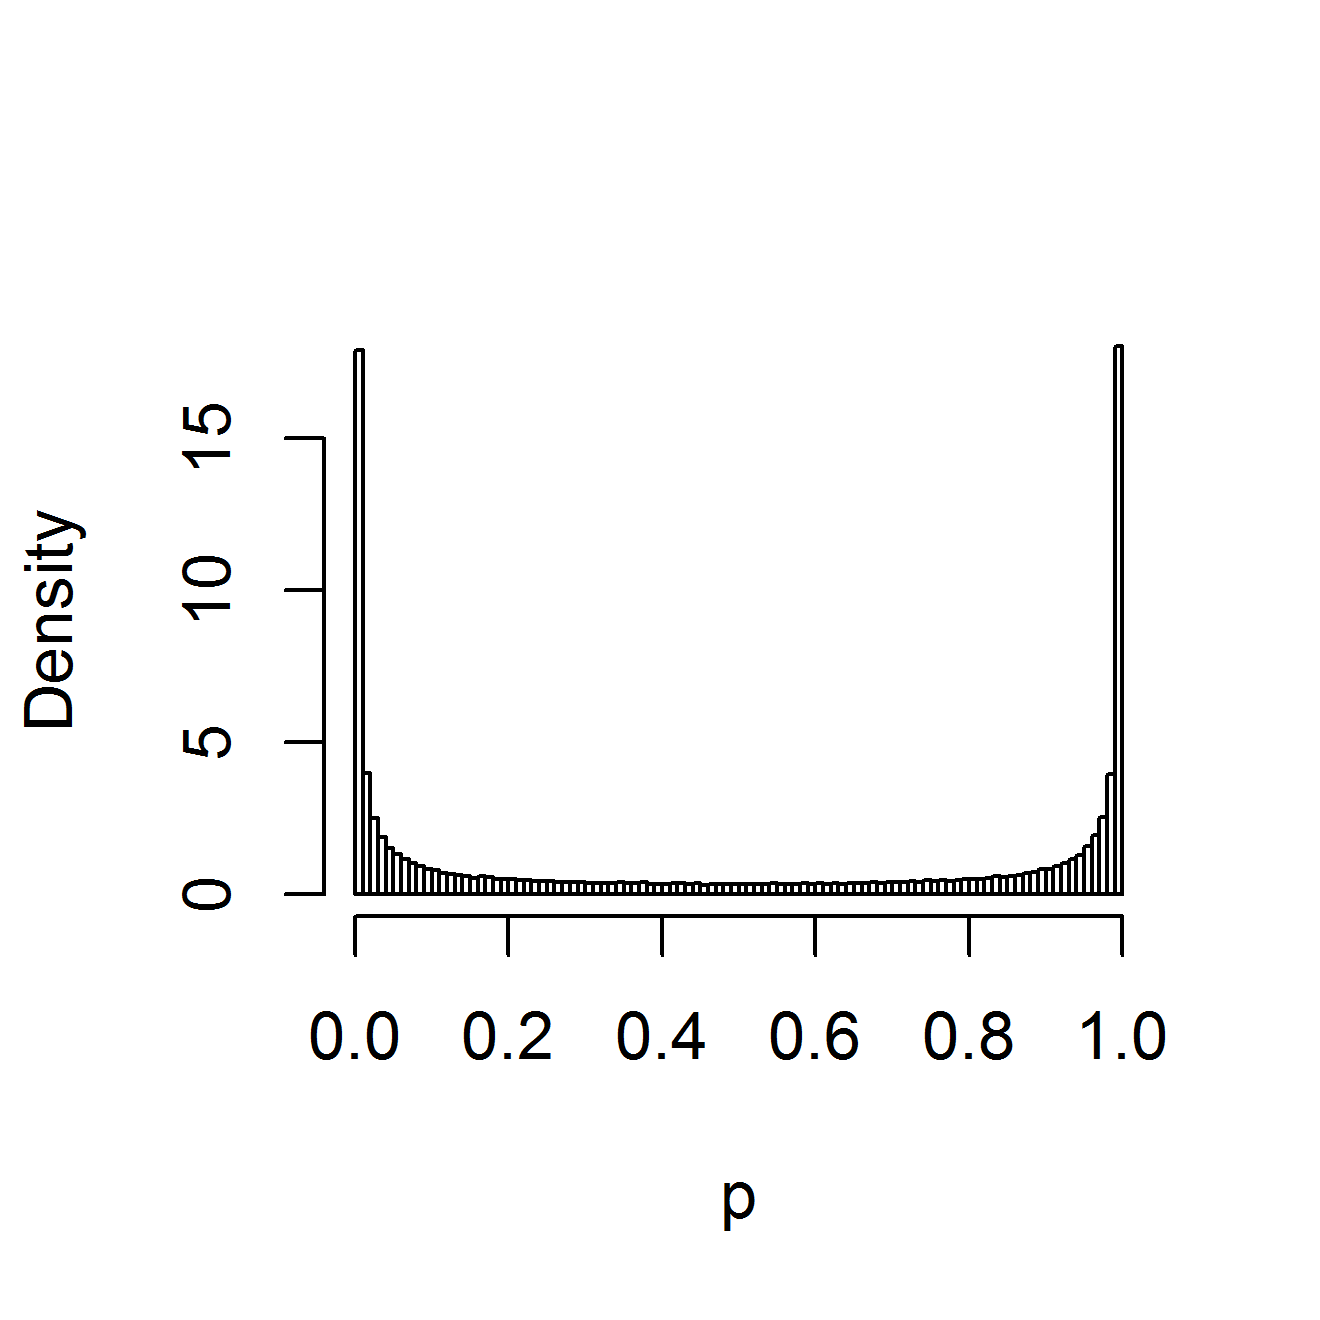
\includegraphics[height=3.0in,width=3.0in]{Ch3-Bayes/figs/implied_prior}
\end{center}
\caption{Implied prior for $p_{0} = \exp(\beta_0)/(1+\exp(\beta_0))$ 
if $\beta_0 \sim \mbox{Normal}(0, 5^2)$.}
\label{glms.fig.impliedprior}
\end{figure}
These two priors can affect results (see Sec. \ref{closed.sec.Mhbear}
for an illustration of this for a real data set), yet they are both
sensible non-informative priors. Despite this, it is often the case
that priors will have little or no impact on the results.
Choice of priors and parameterization
is very much problem-specific and often largely subjective. Moreover,
it also affects the behavior of MCMC algorithms and therefore the
analyst needs to pay some attention to this issue and possibly try
different things out.  Most standard Bayesian analysis books address
issues related to specification and effect of prior distribution
choice in some depth. Some good references include
\citet{kass_wasserman:1996}, \citet{gelman:2006} and
\citet{link_barker:2010}.


\subsection{Convergence and so-forth}
\label{glms.sec.convergence}

Once we have carried out an analysis by MCMC, there are many other
practical issues that we have to confront. One characteristic of MCMC sampling is that Markov chains take some time to converge to their stationary distribution - in our case the posterior distribution for some parameter given data, $[\theta|y]$. Only when the Markov chain has reached
its stationary distribution, the generated samples can be used to
characterize the posterior distribution. Thus, one of the most important issues we need to address 
is ``have the chains converged?'' Since we do not know what the
stationary posterior distribution of our Markov chain should look like
(this is the whole point of doing an MCMC analysis), we
effectively have no means to assess whether or not it has truly converged to
this desired distribution. Most MCMC algorithms only guarantee
that, eventually, the samples being generated will be from the target
posterior distribution, but no-one can tell us how long this will
take. Also, you only know the part of your posterior distribution that
the Markov chain has explored so far -- for all you know the chain
could be stuck in a local maximum, while other maxima remain
completely undiscovered.  Acknowledging that there is truly nothing we
can do to ever prove convergence of our MCMC chains, there are several
things we can do to increase the degree of confidence we have about
the convergence of our chains. Some problems are easily detected using
simple plots, such as a time-series plot, where parameter values of each MCMC iteration are plotted against the number of iterations.  Fig. \ref{glms.fig.linreg} shows the time series plots for the three parameters -- $\beta_0$, $\beta_1$ and $\sigma$ -- from our linear regression example, taken from the {\bf WinBUGS} GUI before closing it to return to {\R}. 

\begin{figure}[ht]
\begin{center}
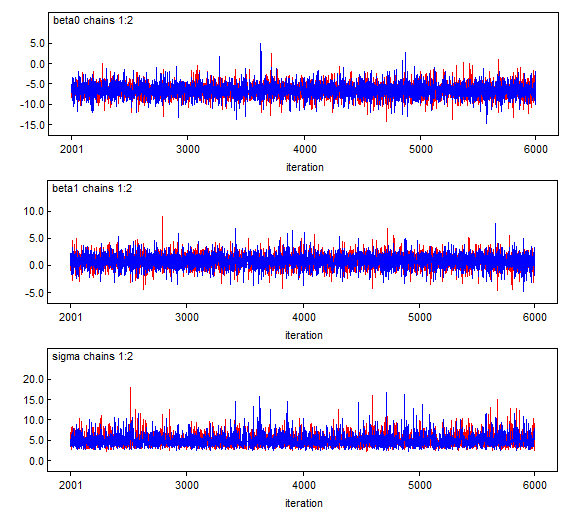
\includegraphics[height=3in]{Ch3-Bayes/figs/BUGSchains}
\end{center}
\caption{
Time-series plots for parameters from a linear regression run in {\bf WinBUGS} using two parallel Markov chains.}
\label{glms.fig.linreg}
\end{figure}

Typically a period of transience is observed in the
early part of the MCMC algorithm, and this is usually discarded as the
``burn-in'' period. In our linear regression example, within the {\tt bugs()} call we set the burn-in period as 2000 iterations so these are automatically removed by {\bf WinBUGS} and are not part of the output (but Fig. \ref{glms.fig.poissonmcmc2} shows a time-series plot that starts at iteration 0 with a clearly visible burn-in period). The quick diagnostic to whether convergence has
been achieved is that your Markov chains look ``grassy'' -- this seems a reasonable statement for the plots in Fig. \ref{glms.fig.linreg}.  Another way to check convergence is to
update the parameters some more and see if the posterior changes. If
the chains have converged to the posterior, 
the posterior mean,
confidence intervals, and other summaries should be relatively static
as we continue to run the algorithm.  Yet
another option, and one generally implemented in {\bf WinBUGS}, is to
run several Markov chains and to start them off at different initial
values that are over-dispersed relative to the posterior
distribution. Such initial values help to explore different areas of
the parameter space simultaneously; if, after a while, all chains
oscillate around the same average value, chances are good that they
indeed converged to the posterior distribution.
\begin{comment}
%%%%%\footnote{Running
  several parallel chains is computationally expensive. But extra
  computational demands are not the only and by no means the major
  concern some people voice when it comes to running several parallel
  MCMC chains to assess convergence. Again, consider the fact that we
  do not know anything about the true form of the posterior
  distribution we are trying to approximate. How do we, then, know how
  to pick over-dispersed initial values? We don't. All we can do is
  pick over-dispersed values relative to our expectations of what the
  posterior should look like. To use a quote from the home page of
  Charlie Geyer, a Bayesian statistician from the University of
  Minnesota, ``If you don't know any good starting points [...], then
  restarting the sampler at many bad starting points is [...] part of
  the problem, not part of the solution.''
  (\url{''http://users.stat.umn.edu/~charlie/mcmc/diag.html''}). His suggestion
  is that your only chance to discover a potential problem with your
  MCMC sampler is to run it for a very long time. But again, there is
  no way of knowing how long is long enough.  It is up to you to
  decide, which school of thoughts appeals more to you, one long
  versus several parallel Markov chains. Irrespectively, part of
  developing an MCMC sampler should be to make sure (within reasonable
  limits) that you are not missing regions of high posterior density
  because of the way you specify your starting values. Once you have
  explored the behavior of your chain under a reasonable range of
  starting values, you may feel comfortable enough to run only one
  long chain.}
\end{comment}
Gelman and Rubin came up with the so-called ``R-hat''
statistic ($\hat{R}$) or Brooks-Gelman-Rubin statistic that
essentially compares within-chain and between-chain variance to check
for convergence of multiple chains \citep{gelman_etal:1996}. The R-hat statistic
should be close to 1 if the Markov chains have converged and
sufficient posterior samples have been obtained. For the linear regression example, we ran two parallel chains (also specified in the {\tt bugs()} call) and {\bf WinBUGS} returns the $\hat{R}$ statistic for us as part of the summary model output. If you look back to Sec. \ref{GLMM.sect.linear} you see that $\hat{R} = 1$ for all parameters of the linear model.
In practice, $\hat{R}
\leq 1.2$ may be good enough for some problems.  For some models you
can't actually realize a low $\hat{R}$. E.g., if the posterior is a
discrete mixture of distributions then you can be misled into thinking
that your Markov chains have not converged when in fact the chains are
just jumping back and forth in the posterior state-space. This happens
in some of indicator variable model selection discussed in Chapt. \ref{chapt.gof}.
%So, for example, model
%selection methods (section XYZ) sometimes suggests non-convergence.
Often, when there is little information about a parameter in the data,
or when parameters are on the boundary of the parameter space,
convergence will appear to be poor also.
These kinds of situations 
are normally ok and you need to think really hard about
the context of the model and the problem before you conclude that your
MCMC algorithm is ill-behaved.

Some models exhibit ``poor mixing'' of the Markov chains (or ``slow
convergence'') in which case the samples might well be from the
posterior (i.e., the Markov chains have converged to the proper
stationary distribution) but simply mix or move around the posterior
rather slowly. Poor mixing can happen for many reasons -- when
parameters are highly correlated (even confounded), or barely
identified from the data, or the algorithms are very terrible and
probably other reasons as well.

Slow mixing equates to high autocorrelation in the Markov chain - the
successive draws are highly correlated, and thus we need to run the
MCMC algorithm much longer to get an effective sample size that is
sufficient for estimation, or to reduce the MC error (see below) to a
tolerable level.  A strategy often used to reduce autocorrelation is
``thinning'', where only every $m^{th}$ value of the Markov
chain output is kept. However, thinning is necessarily inefficient from the
stand point of inference - you can always get more precise posterior
estimates by using all of the MCMC output regardless of the level of
autocorrelation \citep{maceachern_berliner:1994,
  link_eaton:2011}. Practical considerations might necessitate
thinning, even though it is statistically inefficient. For example, in
models with many parameters or other unknowns being tabulated, the
output files might be enormous and unwieldy to work with. In such
cases, thinning is perfectly reasonable. In many cases, how well the
Markov chains mix is strongly influenced by parameterization,
standardization of covariates, and the prior distributions being
used. Some things work better than others, and the investigator should
experiment with different settings and remain calm when things don't
work out perfectly.
% MCMC is an art, as much as it is a science.


{\bf Is the posterior sample large enough?}  The subsequent samples
generated from a Markov chain are not {\it independent} samples from the
posterior distribution, due to the correlation among samples
introduced by the Markov process\footnote{In case you are not familiar
  with Markov chains, for $T$ random samples $\theta^ {(1)}$,
  ... $\theta^{(T)}$ from a Markov chain the distribution of
  $\theta^{(t)}$ depends only on the immediately preceding value,
  $\theta^{(t-1)}$.} and the sample size has to be adjusted to account
for the autocorrelation in subsequent samples (see Chapt. 8 in
\citet{robert_casella:2010} for more details). This adjusted sample
size is referred to as the effective sample size. Checking the degree
of autocorrelation in your Markov chains and estimating the effective
sample size your chain has generated should be part of evaluating your
model output. {\bf WinBUGS} will automatically return the effective
sample size for all monitored parameters, as we saw in our linear regression example (the ``n.eff'' column of the summary output). If you find that your
supposedly long Markov chain has only generated a very short effective
sample, you should consider a longer run. What exactly constitutes a
reasonable effective sample size is hard to say. A more palpable
measure of whether you've run your chain for enough iterations is the
time-series or Monte Carlo error - the ``noise'' introduced into your
samples by the stochastic MCMC process. The MC error is printed by default in summaries produced in the {\bf
  WinBUGS} GUI, which can be reproduced in {\bf R} using {\tt bugs.log('log.txt')\$stats} (note that ``log.txt'' refers to a model log file that {\bf
  WinBUGS} automatically creates in the working directory; it is overwritten with every new model you run unless you save it under a different name).
 
{\small
\begin{verbatim}
> bugs.log('log.txt')$stats
$stats
             mean      sd   MCerror    2.5%   median   97.5% start sample
beta0    -6.64700 1.60300 0.0179400 -9.7140 -6.70800 -3.2730  2001   8000
beta1     0.82100 1.19000 0.0116800 -1.4900  0.82560  3.1800  2001   8000
deviance 58.66000 3.08800 0.0506800 55.0700 57.93000 66.8400  2001   8000
sigma     4.96800 1.52300 0.0248300  2.9350  4.68100  8.7410  2001   8000
tau       0.05074 0.02677 0.0003651  0.0131  0.04564  0.1162  2001   8000
\end{verbatim}
}
  When using {\bf JAGS} the \mbox{\tt summary} command will automatically produce the MC error (which is called ``Time-series SE'' in {\bf
  JAGS}). You want the MC error to be smallish relative to the magnitude of
the parameter and what smallish means will depend on the purpose of
the analysis. For a preliminary analysis you might settle for a few
percent whereas for a final analysis then certainly less than 1\% is
called for. You can run your MCMC algorithm as long as it takes to
achieve that. A consequence of the MC error is that even for the exact
same model, results will usually be slightly different. Thus, as a good rule of
thumb, you should avoid reporting MCMC results to more than 2 or 3
significant digits!
\begin{comment}
% another attempt to address this issue ineffectively 
Note that MC error in summaries of the
posterior is not the same as having an ``approximate'' solution in a
standard likelihood analysis or similar.  The approximate SE in
likelihood inference is actually wrong in its actual value.... XYZ.
\end{comment}

\subsection{Bayesian confidence intervals}

The 95\% Bayesian confidence interval based on percentiles of the
posterior is not a unique interval - there are many of them. The 
so-called ``highest posterior density'' (HPD) interval is an
alternative, defined as the
narrowest interval that contains {\it at least} 95\% of the posterior
mass.  As a result (of the {\it at least} clause), for discrete
parameters, the 95\% HPD is not often exactly 95\% but usually
slightly more conservative than nominal.

\subsection{Estimating functions of parameters}

A benefit of analysis by MCMC is that we can seamlessly estimate
functions of parameters by simply tabulating the desired function of
the simulated posterior draws. For example, if $\theta$ is the
parameter of interest and let $\theta^{(i)}$ for $i=1,2,\ldots,M$ be
the posterior samples of $\theta$. Let $\eta = \exp(\theta)$, then a
posterior sample of $\eta$ can be obtained simply by computing
$\exp(\theta^{(i)})$ for $i=1,2,\ldots,M$. 
Almost all SCR models in this book involve at least 1 derived
parameter. For example, density $D$ is a derived parameter, being a
function of population size $N$ and the area $A$ of the underlying
state-space of the point process (see Chapt. \ref{chapt.scr0}).

{\bf Example: Finding the optimum value of a covariate.}
As another example of estimating functions of model parameters, suppose that the
normal regression model from Sec. \ref{GLMM.sect.linear} had a quadratic response function of the
form
\[
	\mathbb{E}(y_i) = \beta_0 + \beta_1 x_i + \beta_2 x_{i}^{2}.
\]
Then the optimum value of $x$, i.e., that corresponding to the optimal
expected response, can be found by setting the derivative of
this function to 0 and solving for $x$. We find that
\[
df/dx = \beta_1 +
2*\beta_2 x = 0
\]
yields that $x_{opt} = -\beta_1/(2*\beta_2)$.  We can just
take our posterior draws for $\beta_1$ and $\beta_2$ and obtain a
posterior sample of $x_{opt}$ by this simple calculation applied to
the posterior output. As an exercise, take
the normal model above and simulate a quadratic response and then
describe the posterior distribution of $x_{opt}$.


\section{Poisson GLMs}
\label{glms.sec.poisson}

The Poisson GLM (also known as ``Poisson regression'') is probably the
most relevant and important class of models in all of ecology. The
basic model assumes observations $y_{i}; i=1,2,...,n$ follow a Poisson
distribution with mean $\lambda$ which we write
\[
 	y_{i} \sim \mbox{Poisson}(\lambda)
\]
Commonly $y_{i}$ is a count of animals or plants at some point in
space (``site'') $i$, and $\lambda$ might vary over sites as well. For example, $i$ might index point
count locations in a forest, survey route centers, or sample quadrats, or
similar, and we are interested in how $\lambda$ depends on site
characteristics such as habitat.  If covariates are available it is typical to model them as
linear effects on the log mean. If $x_i$ is some measured covariate
associated with observation $i$, then,
\[
 	\log(x_i) = \beta_0  + \beta_1 x_i
\]

While we only specify the mean of the Poisson model directly, the
Poisson model (and all GLMs) has a ``built-in'' variance which is
directly related to the mean. In this case, $\mbox{Var}(y) = \mathbb{E}(y) =
\lambda$. Thus the model accommodates a linear increase in variance
with the mean.

%Richard: move to Ch2
% \subsection{Important properties of the Poisson distribution}
% \label{glms.sec.properties}

% There are two properties of the Poisson distribution
% that make it extremely useful in ecology. First
% is the property of {\it compound additivity}. If $y_1$ and $y_2$ are
% Poisson random variables with means $\lambda_1$ and $\lambda_2$,
% then their sum $N=y_1+y_2$ is Poisson with mean $\lambda_1+\lambda_2$. Thus,
% if the observations can be viewed as an aggregate of counts over some
% finer unit of measurement, then the Poisson mean aggregates in a corresponding
% manner. This comes in hand in some ecological applications
% where we have counts, $y_{i}$, made on sample units with different but known areas $A_{i}$. 
% Then, we might assume 
% the counts have a Poisson distribution with mean $A_{i}\lambda$. On the log-scale we see that 
% $log(A_{i})$ enters as an additive constant -- usually referred to as the ``offset'' in GLM
% lingo. 
% A second useful property of the Poisson distribution is its
% direct relationship to the multinomial.
% If $y_1$ and $y_2$ are $iid$ Poisson then,
% conditional on their sum $N = y_1 + y_2$, their joint distribution is multinomial
%  with sample size $N$ and cell probabilities
% $\lambda_1/(\lambda_1+\lambda_2)$ and
% $\lambda_2/(\lambda_1+\lambda_2)$.  As a result of this, most
% multinomial models can be analyzed as a Poisson GLM and {\it vice versa}.
%END section moved to Ch2

\subsection{Example: Breeding Bird Survey Data}

As an example we consider a classical situation in ecology where
counts of an organism are made at a collection of spatial
locations. In this particular example, we have mourning dove 
({\it Zenaida macroura})
counts
made along North American Breeding Bird Survey (BBS) routes in
Pennsylvania, USA. A route consists of 50 stops separated by 0.5
miles. For the purposes here we are defining $y_i$ = route total count
and the sample location will be marked by the center point of the BBS
route.  The survey is run annually and the data set we analyze is
1966-1998. BBS data can be obtained online at \mbox{\tt
  http:\//\//www.pwrc.usgs.gov\//bbs\//}, but the particular chunk of
data we will be using here is also included in the {\tt scrbook}
package ({\tt data(bbsdata)}).
We will make use of the whole data set shortly but for now we're going
to focus on a specific year of counts (1990) for the sake of
building a simple model.
In 1990 there were 77 active routes; this data set contains rows which index the unique route, column 1 is the
route ID, columns 2-3 are the route coordinates (longitude/latitude),
column 4 is a habitat covariate ``forest cover'' (standardized, see
below) and the remaining columns are the yearly counts. Years for
which a survey was not conducted on a route are coded as ``\mbox{\tt NA}'' in the data matrix. We
imagine that this will be a typical format for many ecological
studies, perhaps with more columns representing covariates.  To read
in the data and display the first few elements of the data frame containing the counts, do
this:
{\small
\begin{verbatim}
> data(bbsdata)               #  loads data frame 'bbs'
> bbsdata$counts[1:2,1:6]

      X     lon    lat    habitat X66 X67
1 72002 -80.445 41.501 -0.3871372  NA  24
2 72003 -80.347 41.214 -1.0171629  NA  NA
\end{verbatim}
}

It is useful to display the spatial pattern in the observed
counts. For that we use a spatial dot plot -- where we plot the
coordinates of the observations and mark the color of the plotting
symbol based on the magnitude of the count.  We have a special
plotting function for that which is called \mbox{\tt spatial.plot()}
and it is available with the supplemental {\bf R} package \mbox{\tt
  scrbook}.  Actually, what we want to do here is plot the log-counts
(+1 of course) which (Fig. \ref{glms.fig.padovecounts}) display a
notable pattern that could be related to something. The {\bf R}
commands for obtaining this figure are: 
{\small
\begin{verbatim}
> library(scrbook)
> data(bbsdata)
> library(maps)

> y <- bbsdata$counts[,"X90"]  # pick out 1990
> notna <- !is.na(y)
> y <- y[notna]
> locs <- bbsdata$counts[notna,c("lon","lat")]
> sz <- y/max(y)

> par(mar=c(3,3,3,6))
> plot(locs,pch=" ",axes=FALSE,xlim=range(locs[,1])+c(-.3,+.3),
     ylim=c(range(locs[,2]) + c(-.6,.6)), xlab=" ",ylab=" ")
> map('state', regions='pennsylvania', add=TRUE, lwd=2)
> spatial.plot(bbsdata$counts[notna,2:3], y, cx=1+sz*6, add=TRUE)
\end{verbatim}
}
We can ponder the potential effects that
might lead to dove counts being high - corn fields, telephone wires,
barn roofs along with misidentification of pigeons, these could all
correlated reasonably well with the observed count of mourning doves.
Unfortunately we don't have any of that information.
\begin{figure}[ht]
\begin{center}
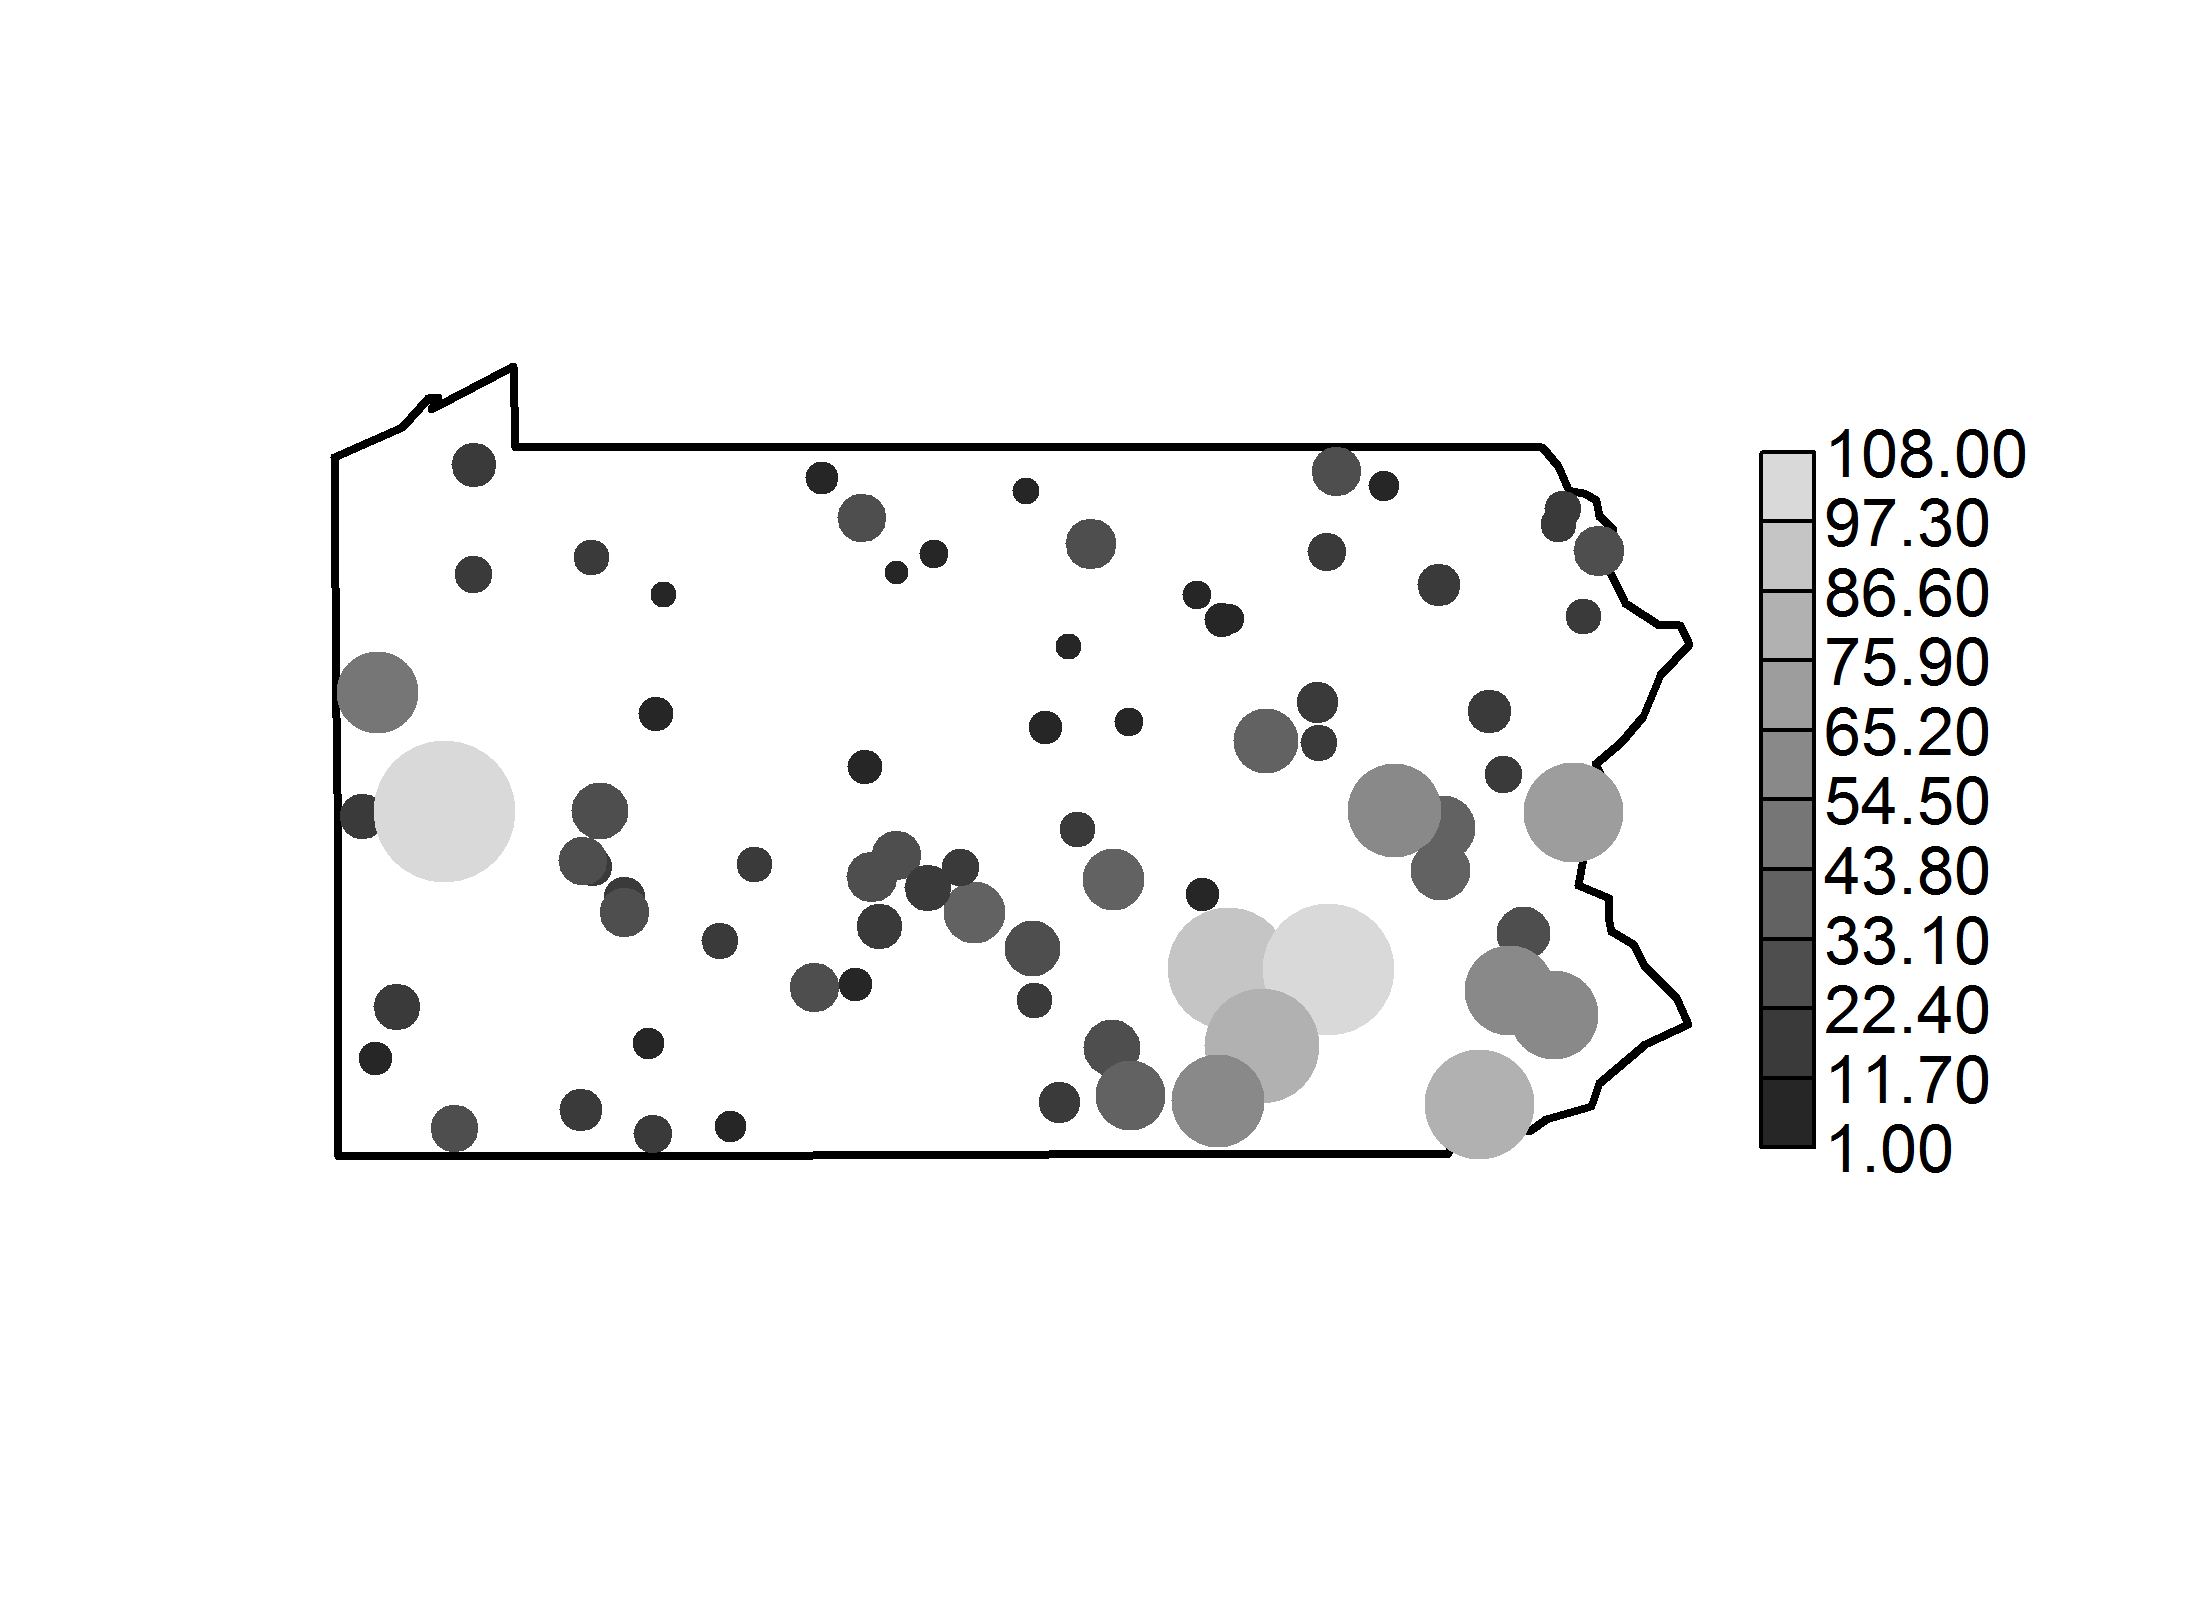
\includegraphics[height=2.75in]{Ch3-Bayes/figs/pacounts}
\end{center}
\caption{ Mourning dove counts along North American Breeding Bird
  Survey routes in Pennsylvania (year = 1990). Plot symbol shading and
  circle size is proportional to raw count. }
\label{glms.fig.padovecounts}
\end{figure}
However, we do have a measure of forest cover (provided in the data frame
\mbox{\tt bbsdata\$habitat}) which can be plotted using the 
\mbox{\tt spatial.plot} function with the following {\bf R} commands
{\small
\begin{verbatim}
>habdata<-bbsdata$habitat
>map('state',regions="penn",lwd=2)
>I<-matrix(NA,nrow=30,ncol=40)
>I<- matrix(habdata[,"dfor"],ncol=40,byrow=FALSE)
>ux<-unique(habdata[,2])
>uy<-sort(unique(habdata[,3]))

>par(mar=c(3,3,3,6))
>plot(locs,pch=" ",axes=FALSE,xlim=range(locs[,1])+c(-.3,+.3),
     ylim=c(range(locs[,2]) + c(-.6,.6)),xlab=" ",ylab=" ")
>image(ux,uy,rot(I),add=TRUE,col=gray(seq(3,17,,10)/20) )
>map('state',regions='pennsylvania',add=TRUE,lwd=3,col="white")
>image.scale(I,col=gray(seq(3,17,,10)/20) )
>points(locs,pch=20,col="white")
\end{verbatim}
}
{\flushleft The} result appears in Fig. \ref{glms.fig.paforest}.
We see a prominent pattern that indicates high forest coverage in the
central part of the state and low forest cover in the SE.  Inspecting
the previous figure of the raw counts suggests a relationship between
counts and forest cover which is perhaps not surprising.
\begin{figure}
\begin{center}
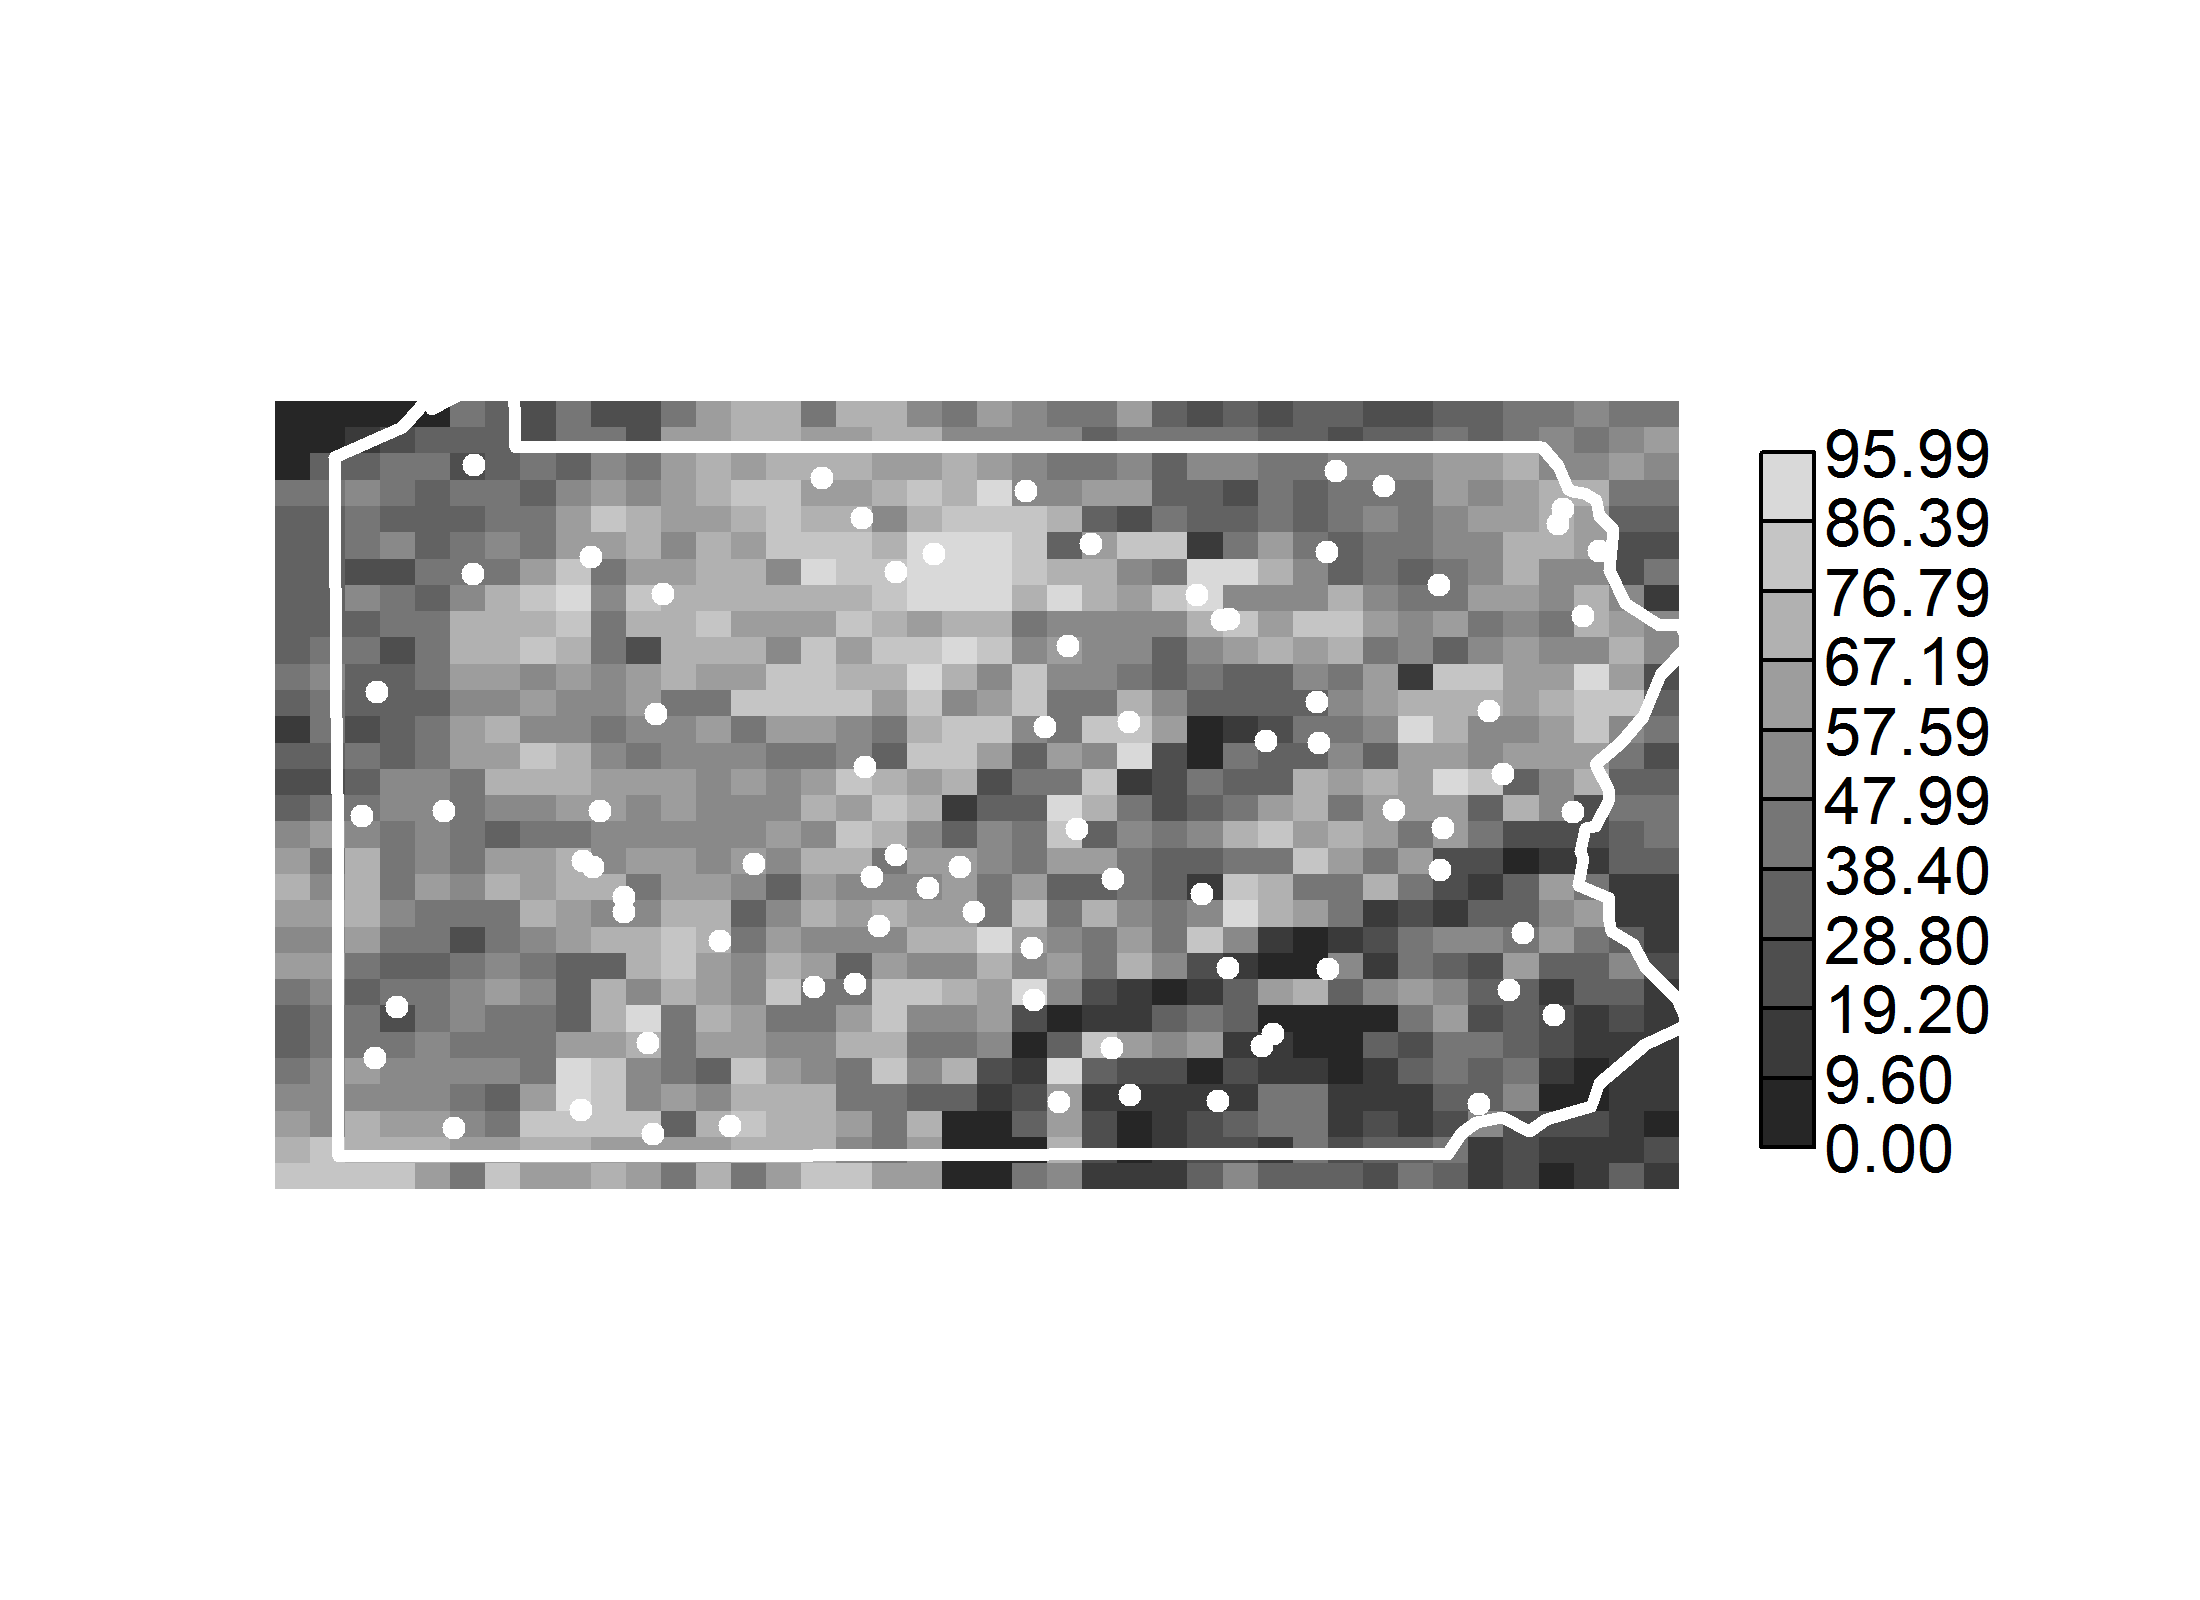
\includegraphics[height=2.75in]{Ch3-Bayes/figs/paforest}
\end{center}
\caption{Forest cover (percent deciduous) in Pennsylvania. BBS route
  locations are shown by white dots. }
\label{glms.fig.paforest}
\end{figure}

\subsection{Doing it in WinBUGS}

Here we demonstrate how to fit a Poisson GLM in {\bf WinBUGS} using the
covariate $x_{i} =$ forest cover along BBS route $i$. It is advisable that $x_i$ be
standardized in most cases as this will improve mixing of the Markov
chains. We have pre-standardized the forest cover covariate for the
BBS route locations,
 and so we don't have to worry about that
here.  To read the BBS data into {\bf R} and get things set up for
{\bf WinBUGS}
we issue the following commands:
{\small
\begin{verbatim}
> library(scrbook)
> data(bbsdata)

> y <- bbsdata$counts[,"X90"]               # pick out 1990
> notna <- !is.na(y)
> y <- y[notna]
## forest cover already standardized here:
> habitat <- bbsdata$counts[notna,"habitat"]
> M <- length(y)

> library(R2WinBUGS)                        # load R2WinBUGS
> data <- list (y=y, M=M, habitat=habitat)  # bundle data for WinBUGS
\end{verbatim}
}
Now we write out the Poisson model specification in {\bf WinBUGS}
pseudo-code, provide initial values, identify parameters to be
monitored and then execute {\bf WinBUGS}:
{\small
\begin{alltt}
> cat("
model\{
    for (i in 1:M)\{
      y[i] \(\sim\) dpois(lam[i])
      log(lam[i]) <- beta0+beta1*habitat[i]
     \}
 beta0 \(\sim\) dunif(-5,5)
 beta1 \(\sim\) dunif(-5,5)
\}
",file="PoissonGLM.txt")
\end{alltt}
}
{\small
\begin{verbatim} 
> inits <- function()  list ( beta0=rnorm(1),beta1=rnorm(1) )
> parameters <- c("beta0","beta1")
> out <- bugs(data, inits, parameters, "PoissonGLM.txt", n.thin=2,n.chains=2,
          n.burnin=2000,n.iter=6000,debug=TRUE,working.dir=getwd())
\end{verbatim}
}
%Note the close correspondence in how the model is
%specified here compared with the normal regression model
%previously. As an exercise you should discuss the specific differences
%between the {\bf BUGS} model specifications for the normal and Poisson
%models. 

% Model output is summarized in table \ref{glms.tab.poisreg}. 
% \begin{table}
% \caption{Inference for Poisson GLM, fit using WinBUGS,
%  2 chains, each with 6000 iterations (first 2000 discarded), n.thin = 2
%  n.sims = 4000 iterations saved.}
%    \scriptsize
%   \begin{tabular}{lccccccccc}
%     \hline
%         \hline
%  Parameter &    mean   & sd   &  2.5\%    &  25\%  &    50\%   &   75\%  &  97.5\% & Rhat & n.eff \\
%      \hline
% beta0  &     3.152 & 0.025  &  3.103  &  3.135  &  3.152  &  3.168 &  3.199 & 1.001 & 4000 \\
% beta1  &    -0.497 & 0.021 & -0.537 &  -0.511 &  -0.497 &  -0.484 &  -0.456 & 1.001 & 4000 \\
% deviance & 1116.576 & 1.997 & 1115.000 & 1115.000 & 1116.000 & 1117.000 & 1122.000 & 1.002 & 4000 \\
%     \hline
%   \end{tabular}
%   \label{glms.tab.poisreg}
% \vspace{0.5cm}
% \end{table}
% since I guess this is the first BUGS analysis we might keep the actual output here. 

{\flushleft The} {\bf WinBUGS} output can be viewed in {\bf R} using the {\tt print} command:
{\small
\begin{verbatim}
print(out,digits=2)
Inference for Bugs model at "PoissonGLM.txt", fit using WinBUGS,
 2 chains, each with 6000 iterations (first 2000 discarded), n.thin = 2
 n.sims = 4000 iterations saved
            mean   sd    2.5%     25%     50%     75%   97.5% Rhat n.eff
beta0       3.15 0.02    3.10    3.13    3.15    3.17    3.20    1  4000
beta1      -0.50 0.02   -0.54   -0.51   -0.50   -0.48   -0.46    1  4000
deviance 1116.56 1.95 1115.00 1115.00 1116.00 1117.00 1122.00    1  4000
\end{verbatim}
}

% We might wonder whether this model provides an adequate fit to our
% data.  To evaluate that, we used a Bayesian p-value analysis with fit
% statistic based on the Freeman-Tukey residual by replacing the model
% specification above with this:
% {\small
% \begin{verbatim}
% cat("
% model {
%     for (i in 1:M){
%       y[i]~dpois(lam[i])
%       log(lam[i])<- beta0+beta1*habitat[i]
%       d[i]<-  pow(pow(y[i],0.5)-pow(lam[i],0.5),2)   #

%       ynew[i]~dpois(lam[i])
%       dnew[i]<-pow( pow(ynew[i],0.5)-pow(lam[i],0.5),2)

%      }
%  fit<-sum(d[])
%  fitnew<-sum(dnew[])
%  beta0~dunif(-5,5)
%  beta1~dunif(-5,5)
% }
% ",file="PoissonGLM.txt")
% \end{verbatim}
% }
% The Bayesian p-value is the proportion of times $fitnew > fit$ which,
% for this data set, is 0. This suggests that the basic Poisson model does 
% not fit well.

\subsection{ Constructing your own MCMC algorithm}
\label{GLMM.sect.mcmc}

At this point it might be helpful to suffer through an example
building a custom MCMC algorithm. Here, we develop an MCMC algorithm
for the Poisson regression model, using a Metropolis-within-Gibbs
sampling framework.  Building MCMC algorithms is covered in more
detail in Chapt. \ref{chapt.mcmc} where you can also find step-by-step
instructions for Metropolis-within-Gibbs samplers, should the
following section move through all this material too quickly.

We will assume that the two parameters, $\beta_0$ and $\beta_1$,have diffuse
normal priors, say $[\beta_0] = \mbox{Normal}(0,100)$ and
$[\beta_1]=\mbox{Normal}(0,100)$ where each has {\it standard deviation}
100 (recall that {\bf WinBUGS} parameterizes the normal in terms of $1/\sigma^{2}$).
We need to assemble the relevant elements of the model which are these
two prior distributions and the
likelihood $[{\bf y}|\beta_0,\beta_1] = \prod_{i} [y_i|\beta_0 \beta_1] $ which is,
mathematically, the product of the Poisson pmf evaluated at each $y_i$,
given particular values of $\beta_0$ and $\beta_1$.
Next, we need to identify the full conditionals
$[\beta_0|\beta_1, {\bf y}]$ and $[\beta_1|\beta_0,{\bf y}]$.  We use the all-purpose
rule for constructing full conditionals
(section \ref{glms.sec.rules})
 to discover that:
\[
 [\beta_0|\beta_1,{\bf y}] \propto \left\{ \prod_{i} [y_{i}|\beta_0,\beta_1]\right\}[\beta_0]
\]
Mathematically, the full conditional is of the form
\[
 [\beta_0|\beta_1,{\bf y}] \propto
\left\{ \prod_{i} 
\exp(-\exp(\beta_{0} + \beta_{1} x_{i}))
\exp(\beta_{0} + \beta_{1} x_{i})^{y_{i}}
\right\}
\exp(-\frac{\beta_{0}^2}{2*100})
\]
which you can program as an {\bf R} function with arguments
$\beta_{0}$, $\beta_{1}$ and ${\bf y}$ without difficulty.
The full-conditional for $\beta_{1}$ is:
\[
 [\beta_1|\beta_0,{\bf y}] \propto \left\{ \prod_{i}
   [y_{i}|\beta_0,\beta_1]\right\} [\beta_1]
\]
which has a similar mathematical representation except the prior is
expressed in terms of $\beta_{1}$ instead of $\beta_{0}$.
Remember, we could replace the ``$\propto$'' with ``$=$'' if we
put $[y|\beta_1]$ or $[y|\beta_0]$ in the denominator. But, in general,
$[y|\beta_0]$ or $[y|\beta_1]$ will be quite a pain to compute and, more
importantly, it is a constant as far as the operative parameters
($\beta_0$ or $\beta_1$,
respectively) are concerned. Therefore,
the MH acceptance probability will be the ratio of the
full-conditional evaluated at a candidate draw to that evaluated at the
current value, and so the denominator required to change $\propto$ to $=$
winds up canceling from the MH acceptance probability.

Here we will
use the so-called random walk candidate generator, which is a Normal proposal distribution, so that, for example,
 $\beta_0^{*} \sim \mbox{Normal}(\beta_0^{t},\delta)$ where $\delta$ is
 the standard-deviation of the proposal distribution, which is just a
 tuning parameter that is set by the user and adjusted to achieve
 efficient mixing of chains (see Sec. \ref{mcmc.sec.mh}).
We remark also that calculations are often done on the log-scale to
preserve numerical integrity of things when quantities evaluate to
small or large numbers, so keep in mind, for example,
$a*b = \exp(\log(a) + \log(b))$ for two positive numbers $a$ and $b$.
 The ``Metropolis within
Gibbs'' algorithm for a Poisson regression turns out to be remarkably
simple and is given in Panel \ref{glms.panel.poisreg}. It is also part
of the {\tt scrbook} package and you can run 1000 iterations of it by
calling {\tt PoisGLMBBS(y=y, habitat=habitat, niter=1000)} (note that
{\tt y} = point count data and {\tt habitat} = forest cover have to
be defined in your {\bf R} workspace as shown in  the previous
analysis of these data).

\begin{panel}[htp]
\centering
\rule[0.15in]{\textwidth}{.03in}
%\begin{minipage}{2.5in}
{\small
\begin{verbatim}
>set.seed(2013)  # so we all get the same result

>out<-matrix(NA,nrow=1000,ncol=2)   # matrix to store the output
>beta0<- -1                         # starting values
>beta1 <- -.8

# begin the MCMC loop ; do 1000 iterations
>for(i in 1:1000){

# update the beta0 parameter
lambda<- exp(beta0+beta1*habitat)
lik.curr<- sum(log(dpois(y,lambda)))
prior.curr<- log(dnorm(beta0,0,100))
beta0.cand<-rnorm(1,beta0,.05)         # generate candidate
lambda.cand<- exp(beta0.cand + beta1*habitat)
lik.cand<- sum(log(dpois(y,lambda.cand)))
prior.cand<- log(dnorm(beta0.cand,0,100))
mhratio<- exp(lik.cand +prior.cand - lik.curr-prior.curr)
if(runif(1)< mhratio)
     beta0<-beta0.cand

# update the beta1 parameter
lik.curr<- sum(log(dpois(y,exp(beta0+beta1*habitat))))
prior.curr<- log(dnorm(beta1,0,100))
beta1.cand<-rnorm(1,beta1,.25)
lambda.cand<- exp(beta0+beta1.cand*habitat)
lik.cand<- sum(log(dpois(y,lambda.cand)))
prior.cand<- log(dnorm(beta1.cand,0,100))
mhratio<- exp(lik.cand + prior.cand - lik.curr - prior.curr)
if(runif(1)< mhratio)
     beta1<-beta1.cand

out[i,]<-c(beta0,beta1)             # save the current values
}

>plot(out[,1],ylim=c(-1.5,3.3),type="l",lwd=2,ylab="parameter value",
     xlab="MCMC iteration")
>lines(out[,2],lwd=2,col="red")
\end{verbatim}
}
%\end{minipage}
\rule[-0.15in]{\textwidth}{.03in}
\caption{
{\bf R} code to run a Metropolis sampler on a simple Poisson regression model.
}
\label{glms.panel.poisreg}
\end{panel}

The first 300 iterations of the MCMC history of each parameter
are shown in Fig. \ref{glms.fig.poissonmcmc2}. These chains are
not very appealing but a couple of things are evident: 
We see
that the burn-in takes about 250 iterations and that after that chains seem to mix 
reasonably well, although this is not so clear given the scale of the
y-axis, which we have chosen to get both variables on the same graph.
We generated 10,000 posterior samples,
discarding the first 500 as burn-in, and the result is shown in
Fig. \ref{glms.fig.grassy}, this time on separate panels for each
parameter.
The ``grassy''
look of the MCMC history is diagnostic of Markov chains that are
well-mixing and we would generally be very satisfied with results that
look like this.

\begin{figure}
\begin{center}
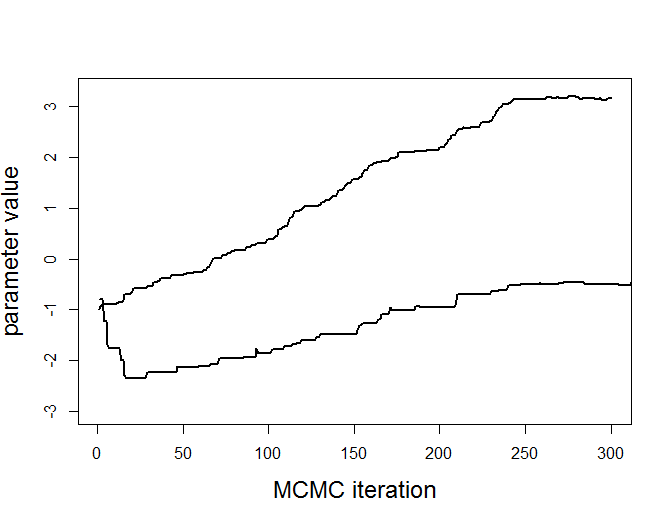
\includegraphics[width=3.5in]{Ch3-Bayes/figs/poissonmcmc2}
\end{center}
\caption{First 300 MCMC iterations for the Poisson GLM model
  parameters $\beta_0$ (top)
and $\beta_1$ (bottom) using
a Metropolis-Hastings tuning parameter of
 $\delta = 0.05$.}
\label{glms.fig.poissonmcmc2}
\end{figure}

\begin{figure}[ht]
\begin{center}
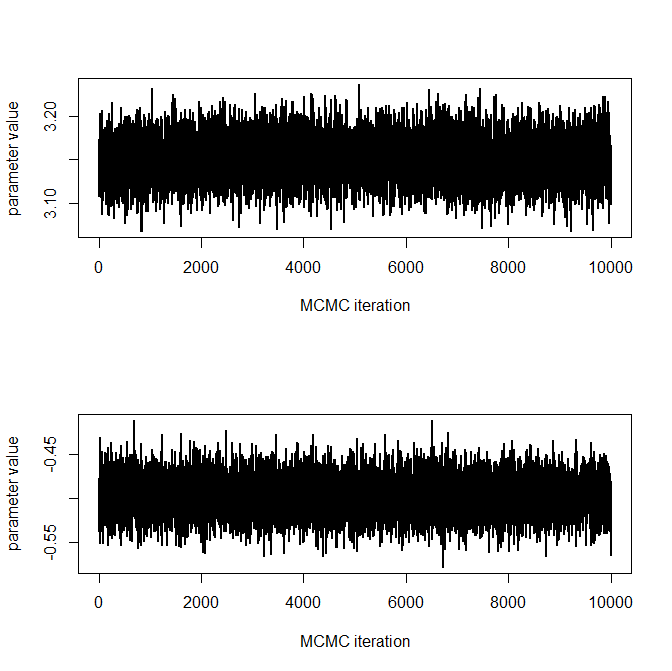
\includegraphics[height=4in,width=5in]{Ch3-Bayes/figs/poissonmcmc3}
\end{center}
\caption{Nice grassy plots of 10,000 MCMC iterations for the Poisson
  GLM model parameters $\beta_0$ (top) and $\beta_1$ (bottom) using a
  Metropolis-Hastings tuning parameter of $\delta = 0.05$.}
\label{glms.fig.grassy}
\end{figure}

Note that we used a specific set of starting values for these
simulations. It should be clear that starting values closer to the
mass of the posterior distribution might cause burn-in to occur
faster. 
%Further, for the diffuse normal prior distributions
%here we could leave the prior contribution out of the full conditional
%evaluation since it is locally constant, i.e., constant in the vicinity of
%the posterior mass, and thus has no practical effect. Removing the
%prior contribution from the MH acceptance probability is equivalent to
%saying that the parameters have an improper uniform prior, i.e.,
%$\beta_0 \sim \mbox{const}$, which is commonly used for mean parameters
%in practice.
Note also that we have
used a different prior than in our {\bf WinBUGS} model specification
given previously. We encourage you to evaluate 
 whether this seems to affect the result.

\section{Poisson GLM with Random Effects}

In most of this book, we will be dealing with random
effects in GLM-like models -- similar to what
are usually referred to as generalized
linear mixed models (GLMMs). We provide a brief introduction of such a
model by way of
example, extending our Poisson regression model to include a random effect.


{\bf The Log-Normal mixture:} The classical situation involves a GLM
with a normally distributed random effect that is additive on the
linear predictor. For the Poisson case, we have:
\[
 	\log(\lambda_{i}) = \beta_0  + \beta_1 x_{i} + \eta_{i}
\]
where $\eta_{i} \sim \mbox{Normal}(0,\sigma^{2})$. In this context, $\eta$ could represent an error term capturing variation in $\lambda_{i}$ not accounted for by the covariates, or overdispersion. 
%A natural
%alternative is to have multiplicative gamma-distributed noise,
%$exp(\eta_{i}) \sim \mbox{Gamma}(a,b)$ which would correspond to a
%negative binomial kind of over-dispersion, implying a different
%mean/variance relationship to the log-normal mixture (the interested
%reader should work that out).  Choosing between such possibilities is
%not a topic we will get into here because it doesn't seem possible to
%provide general guidance on it.   
%% For this model we carried-out a
%% goodness-of-fit evaluation using the Bayesian p-value based on a
%% Pearson residual statistic. See also \citep[][ch. 18]{kery:2010} for
%% an example involving a binomial mixed model\footnote{Kery has noticed
%%   that such tests probably have 0 power. Should use the marginal
%%   frequency of the data}. 
It is really amazingly simple to
express this model in the {\bf BUGS} language and have {\bf WinBUGS}
(or {\bf JAGS}, etc..) draw
samples from the posterior distribution. The code for analysis of the
BBS dove counts is given as follows:
{\small
\begin{alltt}
> library(scrbook)
### grab the BBS Data as before
> data(bbsdata)
### set random seed so that results are repeatable
> set.seed(2013)
### dump the BUGS model into a file
> cat("
model\{
  for (i in 1:M)\{   # observation model, linear predictor, etc..
     y[i] \(\sim\) dpois(lam[i])
     log(lam[i]) <- beta0+ beta1*habitat[i] + eta[i]
     frog[i] <- beta1*habitat[i] + eta[i]
     eta[i] \(\sim\) dnorm(0,tau)
   \}
 ## Prior distributions:
 beta0 \(\sim\) dunif(-5,5)
 beta1 \(\sim\) dunif(-5,5)
 sigma \(\sim\) dunif(0,10)
 tau <- 1/(sigma*sigma)
\}
",file="model.txt")
\end{alltt}
}
{\small
\begin{verbatim}
> data <- list ("y","M","habitat")  # define the data 
> inits <- function()               # inits and parameters to monitor
  list ( beta0=rnorm(1), beta1=rnorm(1), sigma=runif(1,0,4))
> parameters <- c("beta0","beta1","sigma","tau")

> library(R2WinBUGS)                # load and run R2WinBUGS 
> out <- bugs (data, inits, parameters, "model.txt", n.thin=2,n.chains=2,
               n.burnin=1000, n.iter=5000, debug=TRUE)
\end{verbatim}
}

This produces the posterior summary statistics given in table \ref{glms.tab.bbspoisreg}. 
One thing we notice is
that the posterior standard deviations of the regression parameters
are much higher, a result of the extra-Poisson variation allowed for
by this model. We would also
notice much less precise predictions of hypothetical new
observations.



\begin{table}
\caption{Posterior summaries for Poisson GLMM containing a normal random effect
and a  habitat effect for mourning
  dove counts across BBS routes in PA, 1990. Model was fit using 
{\bf WinBUGS},
 2 chains, each with 5000 iterations (first 1000 discarded), n.thin = 2
 n.sims = 4000 iterations saved.}
   \scriptsize
  \begin{tabular}{lrrrrrrrrr}
    \hline
        \hline
 Parameter &    Mean   & SD   &  2.5\%    &  25\%  &    50\%   &   75\%  &  97.5\% & Rhat & n.eff \\
     \hline
$\beta_0$   &   2.98 & 0.08 &  2.82 &  2.93  & 2.98 &  3.03 &  3.12 & 1.00 & 1400 \\
$\beta_1$   &  -0.53 & 0.07 & -0.68 & -0.58 & -0.53 & -0.49 & -0.38 & 1.01 &  350 \\
$\sigma$   &   0.60 & 0.06 &  0.49 &  0.56 &  0.59 &  0.64 &  0.73 & 1.00 & 2000 \\
$\tau$     &   2.88 & 0.57 &  1.88 &  2.47 &  2.86 &  3.24 &  4.12 & 1.00 & 2000 \\
deviance & 445.94 & 12.18 & 424.00 & 437.40 & 445.20 & 453.90 & 471.50 & 1.00 & 4000 \\
    \hline
  \end{tabular}
  \label{glms.tab.bbspoisreg}
\vspace{0.5cm}
\end{table}


% {\small
% \begin{verbatim}
% print(out,digits=2)
% Inference for Bugs model at "model.txt", fit using WinBUGS,
%  2 chains, each with 5000 iterations (first 1000 discarded), n.thin = 2
%  n.sims = 4000 iterations saved
%            mean    sd   2.5%    25%    50%    75%  97.5% Rhat n.eff
% beta0      2.98  0.08   2.82   2.93   2.98   3.03   3.12 1.00  1400
% beta1     -0.53  0.07  -0.68  -0.58  -0.53  -0.49  -0.38 1.01   350
% sigma      0.60  0.06   0.49   0.56   0.59   0.64   0.73 1.00  2000
% tau        2.88  0.57   1.88   2.47   2.86   3.24   4.12 1.00  2000
% deviance 445.94 12.18 424.00 437.40 445.20 453.90 471.50 1.00  4000

% [... some output deleted ...]
% \end{verbatim}
%}
% The Bayesian p-value for this model is
% \begin{verbatim}
% > mean(out$sims.list$fit>out$sims.list$fitnew)
% [1] 0.4815
% \end{verbatim}
% indicating a pretty good fit. Given the site-level random effect, it
% would be surprising for this model to not fit! 




\section{Binomial GLMs}

Another extremely important class of models in ecology are
binomial models. We use binomial models for count data whenever the
observations are counts or frequencies and it is natural to condition
on a ``sample size'', say $K$, the maximum frequency possible in a sample.
 The random variable, $y \le K$, is then the
frequency of occurrences out of $K$ ``trials''. The parameter of the binomial
models is $p$, often called ``success probability'' which is related
to the expected value of $y$ by $\mathbb{E}(y) = pK$. Usually we are interested
in modeling covariates that affect the parameter $p$, and such models
are called binomial GLMs, binomial
regression models or logistic regression, although logistic regression
 really only applies when the logistic link is used to model
the relationship between $p$ and covariates (see below).

One of the most typical binomial GLMs occurs when the sample size
equals 1 and the outcome, $y$, is ``presence'' ($y=1$) or ``absence''
($y=0$) of a species. In this case, $y$ has a Bernoulli distribution. 
This is a classical species distribution
modeling situation. A special situation occurs when presence/absence
is observed with error \citep{mackenzie_etal:2002,tyre_etal:2003}.
In that case, $K>1$ samples
are usually needed for effective estimation of model parameters.

 In standard binomial regression problems the sample size
is fixed by design but interesting models also arise when the sample
size is itself a random variable. These are the $N$-mixture models
\citep{royle:2004biom, kery_etal:2005, royle_dorazio:2008, kery:2010}
and related models (in this case, $N$ being the sample size,
which we labeled $K$ above)\footnote{Some of the jargon is actually a little
bit confusing here
because the binomial index is customarily referred to as ``sample size''
but in the context of $N$-mixture models $N$ is actually the
``population size''}.
Another
situation in which the binomial sample size is ``fixed'' is closed
population capture-recapture models in which a population of
individuals is sampled $K$ times.  The number of times each individual
is encountered is a binomial outcome with parameter (encounter
probability) $p$, based on a sample of size $K$.  In addition, the
total number of unique individuals observed, $n$, is also a binomial
random variable based on population size $N$.  We consider such
models in Chapt. \ref{chapt.closed}.


\subsection{Binomial regression}

In binomial models, covariates are modeled on a suitable
transformation (the link function) of the binomial success
probability, $p$.  Let $x_{i}$ denote some measured covariate for
sample unit $i$ and let $p_{i}$ be the success probability for unit or
subject $i$.
The standard choice is the logit link function (\ref{glms.sec.glmms})
but there are many other possible link functions. 
%However, ecologists seem
%to adopt the logit link function without question in most
%applications\footnote{a notable exception is distance sampling, which
%  is all about choosing among link functions}.  
We sometimes use the
complementary log-log (= ``cloglog'') link function in ecological
applications because it is natural in some cases when the response
should scale in relation to area or effort
\citep[][p. 150]{royle_dorazio:2008}. As an example, the
``probability of observing a count greater than 0'' under a Poisson
model is $\Pr(y>0) = 1-\exp(- \lambda)$. In that case, for the
$i^{th}$ observation,
\[
\mbox{cloglog}(p_{i}) = \log(- \log(1-p_{i})) = \log(\lambda_{i})
\]
so that if you have covariates in your linear predictor for $\mathbb{E}(y)$
under a Poisson model then they are linear on the complementary
log-log link of $p$.
In models of species occurrence it seems natural to view occupancy as
being derived from local abundance $N$
\citep{royle_nichols:2003,royle_dorazio:2006,dorazio:2007}.
Therefore,
models of local abundance in which $N_{i} \sim \mbox{Poisson}(A_{i} \lambda_{i})$
for a habitat patch of area $A_{i}$ implies a model for occupancy $\psi_{i}$
of the form
\[
 \mbox{cloglog}(\psi_{i}) = \log(A_{i}) + \log(\lambda_{i}).
\]
We will use the cloglog link in some analyses of
SCR models in Chapt. \ref{chapt.scr0} and elsewhere.


\subsection{ Example: Waterfowl Banding Data}

The standard binomial modeling problem in ecology is that of 
modeling species distributions, 
 where $K=1$ and the outcome is occurrence ($y=1$) or not
($y=0$) of some species. Such examples abound in books (e.g.,
\citet[][ch. 3]{royle_dorazio:2008}; \citet[][ch. 21]{kery:2010};
\citet[][ch. 13]{kery_schaub:2011}) and in the literature.
Therefore, instead, we will
consider an example involving band returns of waterfowl in the upper great plains including some Canadian provinces, which were
analyzed by \citet{royle_dubovsky:2001}.

For these data, $y_{it}$ is the number of mallard ({\it Anas platyrhynchos}) bands recovered out
of $B_{it}$ birds banded at some location ${\bf s}_{i}$ in year $t$. In this case $B_{it}$ is
fixed. Thinking about recovery rate as being proportional to harvest
rate, we use these data to explore geographic gradients in recovery rate
resulting from variability in harvest pressure experienced by different
populations. 
As such, we fit a
basic binomial GLM with a linear response to geographic coordinates
(including an interaction term). 
% The data ({\tt mallarddata}) are provided with the {\bf
%   R} package \mbox{\tt scrbook}. XXX MAYBE ADD LATER XXXX
Here we
 provide the part of the script for creating the model and fitting the
 model in
{\bf WinBUGS}.
There are few structural differences between this model and the
Poisson GLM fitted previously. The main things are due to the data
structure (we have a matrix here instead of a vector) and otherwise we
change the  distributional assumption to binomial (specified with
\mbox{\tt dbin}) and then use the \mbox{\tt logit} function to relate
the parameter $p_{it}$ to the covariates.  

{\flushleft \bf Dummy variables in BUGS: }
% In
%Chapt. \ref{chapt.modeling} we introduced the concept of categorical
%variables and how to display them in model formulas in the form of
%``dummy variables''. 
In the mallard example, we model the band
recovery probability $p_{it}$ not only as a linear function (on the logit
scale) of geographic location, but also allow for variation in $p_{it}$
with year, $t$; $t=1,2,...T$. In this particular example there are
$T=5$ years of data and we could describe the full mallard
model with a formula in terms of ``dummy variables.'' Dummy variables
are binary
variables, one variable for each level of the categorical variable
they describe, such that variable for level $t$ takes on the value 1
if the observation belongs with level $t$ and 0 otherwise. So, the
mallard model in terms of dummy variables for ``year'' looks like this:
\begin{eqnarray*}
y_{it} &\sim & \mbox{Binomial}(p_{it}, B_{it}) \\
\mbox{logit}(p_{it}) &=& \beta_0 + \beta_1 x_{2,it}+ \beta_2 x_{3,it} +
\beta_3 x_{4,it} + \beta_4 x_{5,it} + 
\beta_5 \mbox{\tt Lat}_i + \beta_6 \mbox{\tt Lon}_i + \beta_7
\mbox{\tt Lat}_i \mbox{\tt Lon}_i
\end{eqnarray*}
Here, $x_{2}$ to $x_{5}$ are the dummy variable vectors of length $T$
that take on the value of 1 when $t$ corresponds to the respective
year and 0 otherwise; $\beta_0$ is the common intercept term and
corresponds to $t=1$; $\beta_1$ - $\beta_4$ describe the difference in
$p_{it}$ for each $t$ relative to $t=1$.

There is a more concise way of implementing such a model with a
categorical covariate in {\bf BUGS}, namely, by using indexing instead
of dummy variables\footnote{Actually, in some cases a model may mix or
  converge better depending on whether you choose a dummy variable or
  an indexing description of it, although they are structurally
  equivalent \citep{kery:2010}}. Essentially, instead of estimating
the difference in $p$ relative to category 1, we estimate a separate
intercept term for each category, so that we have 5 different $\beta_0$
parameters indexed by $t$. This reduces the linear predictor to:
\[
\mbox{logit}(p_{it}) = \beta_{0t} +  \beta_5 \mbox{\tt Lat}_i + \beta_6
\mbox{\tt Lon}_i + \beta_7 \mbox{\tt Lat}_i \mbox{\tt Lon}_i
\]
The model can be implemented in the {\bf BUGS} language for the
mallard banding data using the following {\bf R} script, provided in
the \mbox{\tt scrbook} package (see \mbox{\tt help(mallard)}): 
{\small
\begin{alltt}
> library(scrbook)
> data(mallard)    # load mallard data

> cat("
model\{
 for(t in 1:5)\{
    for (i in 1:nobs)\{
       y[i,t] \(\sim\) dbin(p[i,t], B[i,t])
       pl[i,t] <- beta0[t]+beta1*X[i,1]+beta2*X[i,2]+beta3*X[i,1]*X[i,2]
       p[i,t] <- exp(pl[i,t])/(1+exp(pl[i,t]))
     \}
 \}
	beta1 \(\sim\) dnorm(0,.001)
	beta2 \(\sim\) dnorm(0,.001)
	beta3 \(\sim\) dnorm(0,.001)
	for(t in 1:5)\{
 	beta0[t] \(\sim\) dnorm(0,.001)  
        \}
\}
",file="BinomialGLM.txt")
\end{alltt}
}
{\small
\begin{verbatim}
> library(R2WinBUGS)
> data <- list(B=mallard$bandings, y=mallard$recoveries,
             X=mallard$locs, nobs=nrow(mallard$locs))
> inits <- function(){ list(beta0=rnorm(5),beta1=0,beta2=0,beta3=0) }
> parms <- list('beta0','beta1','beta2','beta3')
> out <- bugs(data, inits, parms,"BinomialGLM.txt", n.chains=3,
              n.iter=2000, n.burnin=1000, n.thin=2, debug=TRUE)
\end{verbatim}
}

\begin{table}
\caption{Posterior summaries for the binomial GLM of mallard band
  recovery rate.  Model contains year-specific intercepts
  ($\beta_{0t}$) and a linear response surface with interaction. 
Model was fit using {\bf WinBUGS}, and posterior summaries are based 
on 3 chains, each with 2000 iterations (first 1000 discarded), n.thin = 2
 n.sims = 1500 iterations saved.
   }
%   \scriptsize
  \begin{tabular}{lrrrrrrr}
    \hline
        \hline
 Parameter &    Mean   & SD   &  2.5\%   &    50\%   &   97.5\% & Rhat & n.eff \\
     \hline
beta0[1] &  -2.346& 0.036&   -2.417&   -2.346&   -2.277& 1.001&  1500\\
beta0[2] &  -2.356& 0.032&   -2.420&   -2.356&   -2.292& 1.001&  1500\\
beta0[3] &  -2.220& 0.035&   -2.291&   -2.219&   -2.153& 1.001&  1500\\
beta0[4] &  -2.144& 0.039&   -2.225&   -2.143&   -2.068& 1.000&  1500\\
beta0[5] &  -1.925& 0.034&   -1.990&   -1.924&   -1.856& 1.004&   570\\
beta1    &  -0.023& 0.003&   -0.028&   -0.023&   -0.018& 1.001&  1500\\
beta2    &   0.020& 0.006&    0.009&    0.020&    0.031& 1.001&  1500\\
beta3    &   0.000& 0.001&   -0.002&    0.000&    0.002& 1.001&  1500\\
deviance &1716.001& 4.091& 1710.000&  1715.000&  1726.000& 1.001&  1500\\
    \hline
  \end{tabular}
  \label{glms.tab.mallard}
\vspace{0.5cm}
\end{table}



Look at the posterior summaries of model parameters in Table
\ref{glms.tab.mallard}. The basic result suggests a negative east-west
gradient and a positive south to north gradient of band recovery
probabilities, but no interaction. A map of the response surface is
shown in Fig. \ref{glms.fig.bandrecovery}.
%  We did an additional MCMC run where we saved the binomial
% parameter $p$ and computed the Bayesian p-value (double use of ``p''
% here is confusing, but I guess that happens sometimes!)
% using a fit statistic based on the Freeman-Tukey
% statistic (see Sec. \ref{glms.sec.gof}
% above). The result indicates that the
% linear response surface model does not provide an adequate fit of the
% data. The reader should contemplate whether this invalidates the basic
% interpretation of the result.


\begin{figure}[ht]
\begin{center}
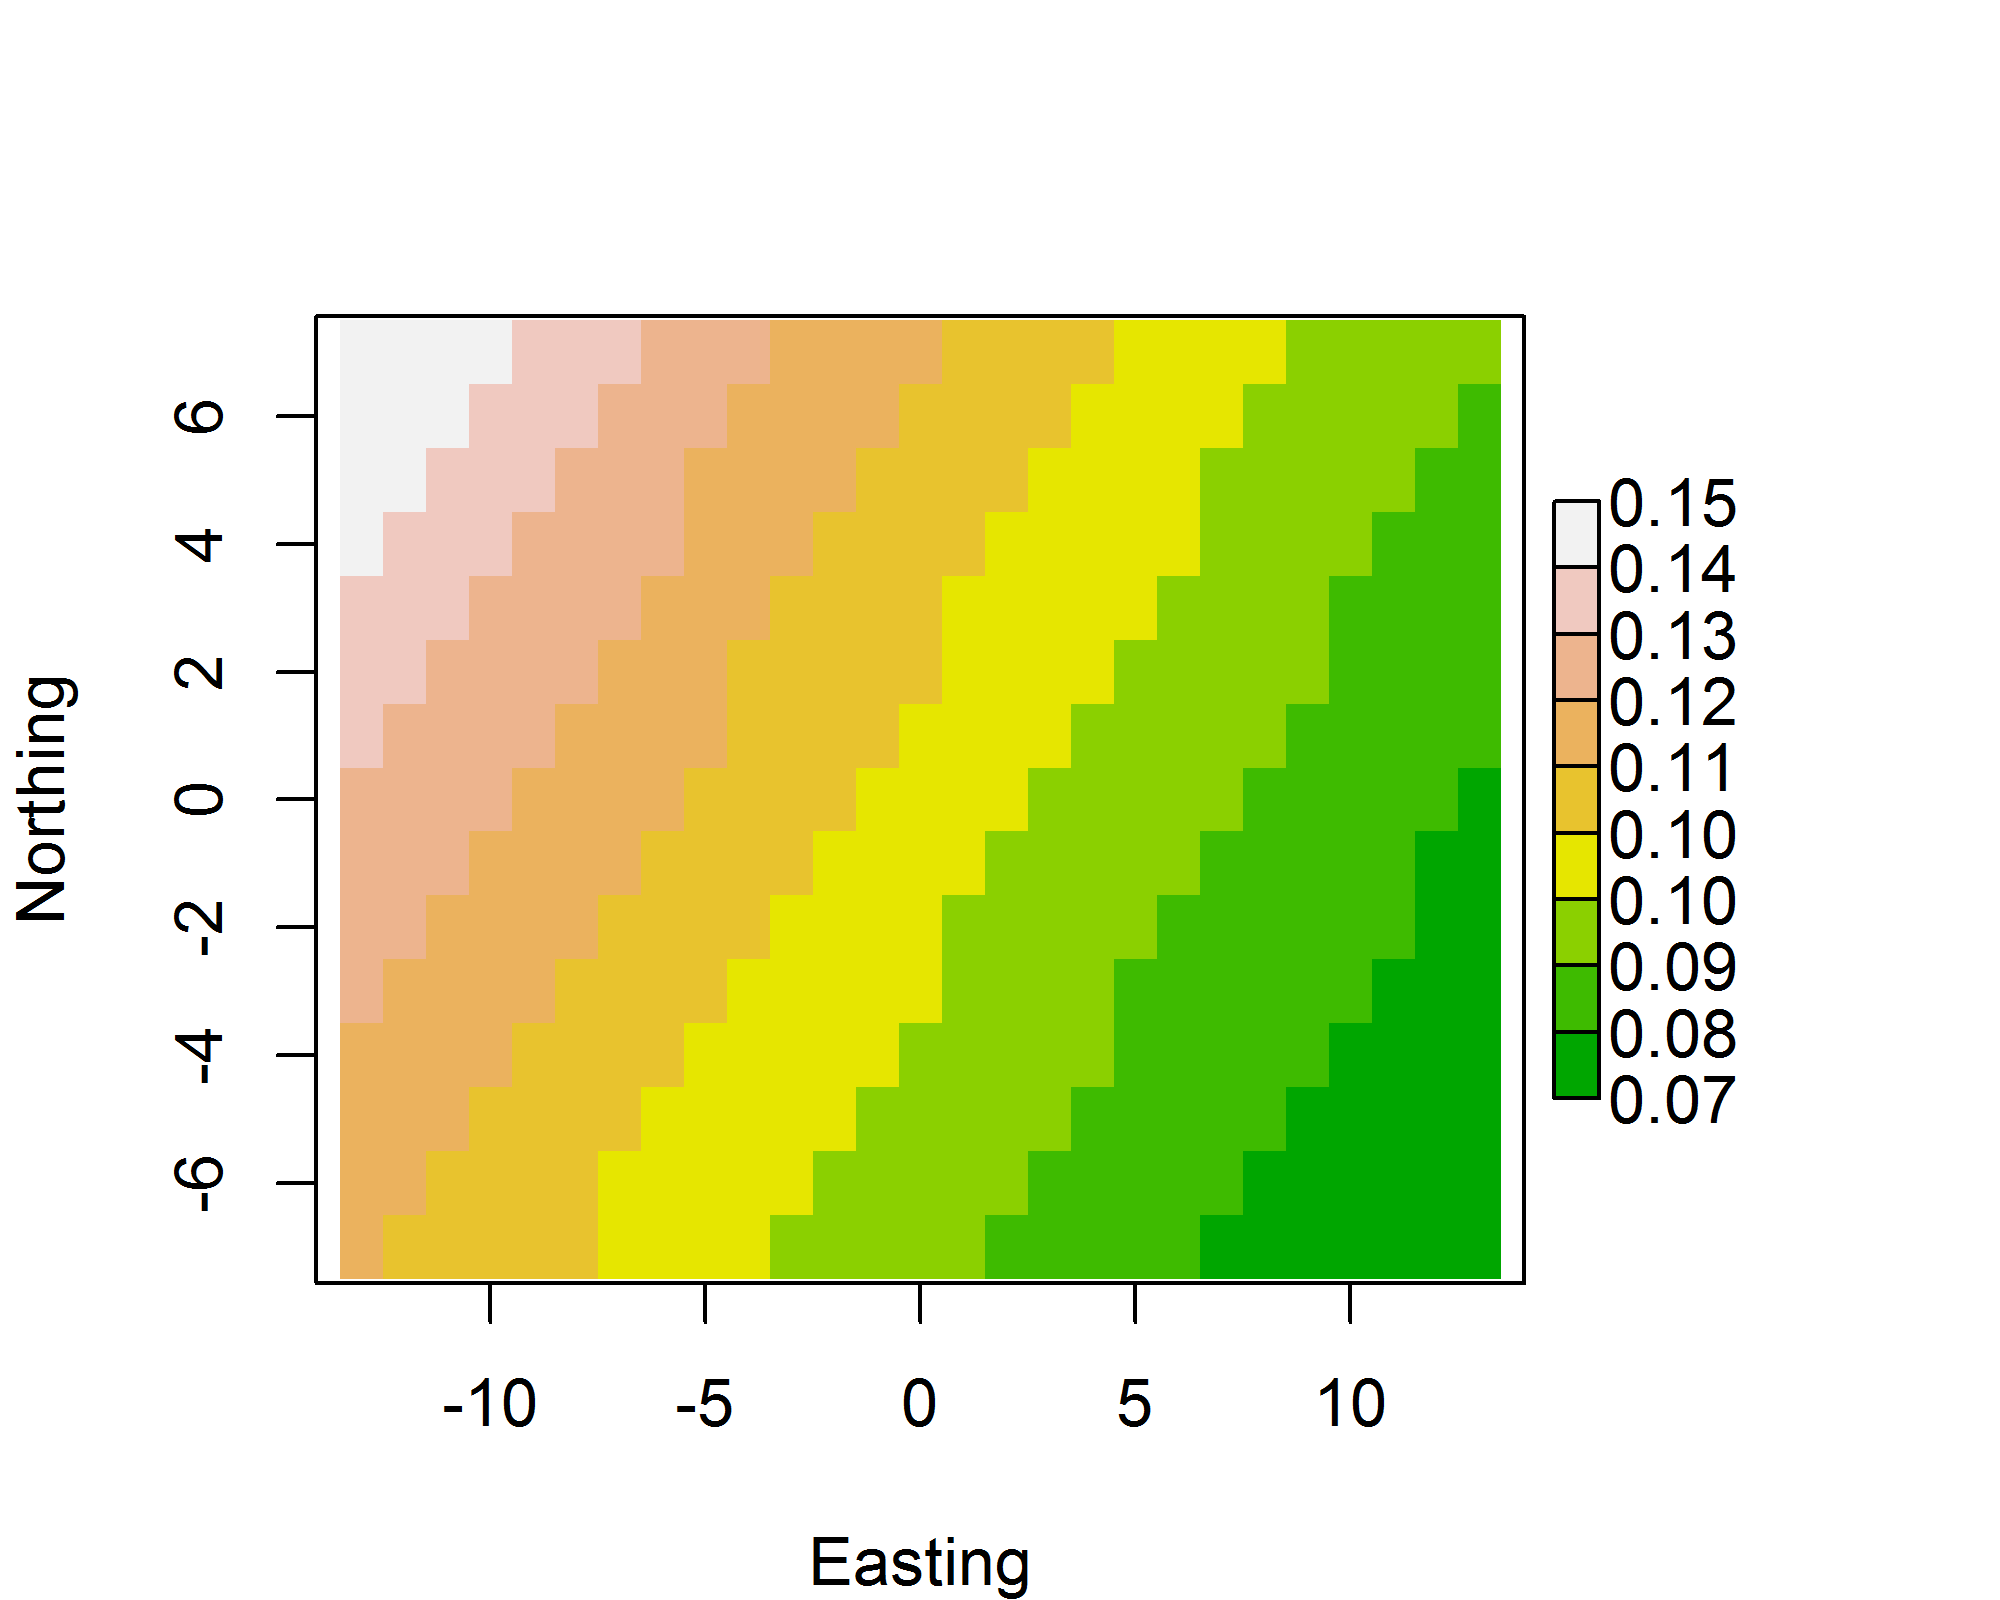
\includegraphics[height=2.5in,width=5in]{Ch3-Bayes/figs/mallard_gradient}
\end{center}
\caption{Predicted recovery rates of mallard bands in the upper great
  plains of North America. Note the negative gradient from the NW to
  the SE.}
\label{glms.fig.bandrecovery}
\end{figure}

\section{Bayesian Model Checking and Selection}
\label{glms.sec.modsel}

In general terms,  model checking -- or assessing the adequacy of the
model -- and model selection are quite thorny issues and, despite
contrary and, sometimes, strongly held belief among practitioners, there are not
really definitive, general solutions to either problem. We're against
dogma on these issues and think people need to be open-minded about
such things and recognize that models can be useful whether or not
they pass certain statistical tests. Some models are intrinsically
better than others because they make more biological sense or foster
understanding or achieve some objective that some  bootstrap
or other goodness-of-fit test can't decide for you. That said, it
gives you some confidence if your model seems adequate in a purely statistical
sense.
We provide a very brief overview of concepts here, but provide more
detailed coverage in Chapt. \ref{chapt.gof}.
See also coverage of these topics in
\citet[][]{kery:2010} and
\citet[][]{link_barker:2010}
for specific context related to Bayesian
model checking and selection.

\subsection{Goodness-of-fit}
\label{glms.sec.gof}

Goodness-of-fit testing is an important element of any analysis
because our model represents a general set of hypotheses about the
ecological and observation processes that generated our data. Thus, if
our model ``fits'' in some statistical or scientific sense, then we
believe it to be consistent with the hypotheses that went into the
model. More formally, we would conclude that the data are {\it not
  inconsistent} with the hypotheses, or that the model appears
adequate. If we have enough data, then of course we will reject any
set of statistical hypotheses.  Conversely, we can always come up with
a model that fits by making the model extremely complex. Despite this
paradox, it seems to us that simple models that you can understand
should usually be preferred even if they don't fit, for example if
they embody essential mechanisms central to our understanding of
things, or if we think that some contributing factors to lack-of-fit
are minor or irrelevant to the scientific context and intended use of
the model.  In other words, models can be useful irrespective of
whether they fit according to some formal statistical test of fit.
Yet the tension is there to obtain fitting models, and this comes
naturally at the expense of models that can be easily interpreted and
studied and effectively used.  Unfortunately, conducting a
goodness-of-fit test is not always so easy to do. And, moreover, it is
never really easy (or especially convenient) to decide if your
goodness-of-fit test is worth anything. It might have 0 power!
Despite this, we recommend attempting to assess model fit in real
applications, as a general rule, and we provide some basic guidance
here and some more specific to SCR models in Chapt. \ref{chapt.gof}.

To evaluate goodness-of-fit in Bayesian analyses, we will most often
use the Bayesian p-value \citep{gelman_etal:1996}.  The basic idea is to define
a fit statistic or ``discrepancy measure'' and compare the posterior distribution of that
statistic to the posterior predictive distribution of that statistic
for hypothetical perfect data sets for which the model is known to be correct. For
example, with count frequency data, a standard measure of fit is the
sum of squares of the ``Pearson residuals'',
\[
D(y_i,\theta) = \frac{(y_i - \mathbb{E}(y_i))}{\sqrt{\mbox{Var}( y_{i} )}}
\]
The fit statistic based on the squared residuals computed from the
observations is 
\[
T({\bf y}, \theta) = \sum_{i} D(y_{i},\theta)^{2}
\]
which can be computed at each iteration of a MCMC algorithm given the
current values of parameters that determine the
 response distribution.  At the same time (i.e., at each MCMC
 iteration),
the equivalent statistic is computed for a
``new'' data set, say ${\bf y}^{new}$, 
simulated using the current parameter values. From the new data set,
we compute the same fit statistic:
\[
T({\bf y}^{new}, \theta) = \sum_{i} D(y_{i}^{new},\theta)^{2}
\]
and 
the
Bayesian p-value is simply the posterior probability $\Pr(T({\bf
  y}^{new})  >  T({\bf y}))$
 which should be close to $0.50$ for a good model -- one that
 ``fits'' in the sense that the observed data set is
 consistent with realizations simulated under the model being fitted
 to the observed data. In practice
we judge ``close to 0.50'' as being ``not too close to 0 or 1'' and,
as always, closeness is somewhat subjective. We're happy with anything
$>.1$ and $<.9$ but might settle for $>.05$ and $<0.95$. 
Another useful fit statistic is the Freeman-Tukey
statistic, in which
\[
D({\bf y},\theta) = \sum_{i} ( \sqrt{y_{i}} - \sqrt{\mathbb{E}(y_{i})} )^2
\]
\citep{brooks_etal:2000}, where $y_{i}$ is the observed value of
observation $i$ and $\mathbb{E}(y_{i})$ its expected value. In contrast to a
Chi-square discrepancy, the Freeman-Tukey statistic removes the need
to pool cells with small expected values.
In summary, you can see that 
the Bayesian p-value is easy to compute,
and it is widely used as a result.


\subsection{Model Selection }

In ecology, scientific hypotheses are often manifest as different models or parameters
 of a model, and so
evaluating the importance of different models is fundamental 
to many ecological studies.
For Bayesian model selection we typically use three different methods: First
is, let's say, common sense. If a variable should plausibly be
relevant to explaining the data-generating processes, and it has 
 posterior mass
concentrated away from 0, then it seems like it should be regarded as
important - that is, it is ``significant.''  This approach seems to
have fallen out of favor in ecology over the last 10 or
15 years but in many situations it is a reasonable thing to do.

For regression problems we sometimes use the indicator variable method
of \citet{kuo_mallick:1998}, in 
which we introduce a set of binary variables $I_{k}$ for variable
$k$, and express the model as, e.g., for a single covariate model:
 \[
 \mathbb{E}(y_i) = \beta_0 + I_{1} \beta_1 x_{i}
\]
where $I_{1}$ is given a Bernoulli prior distribution with some prescribed
probability. E.g., $I_{1} \sim \mbox{Bernoulli}(0.50)$ to provide a prior probability
of 0.50 that variable $x$ should be an element of the linear
predictor. The posterior probability of the event $I_{1}=1$ is a gage of
the importance of the variable $x$. i.e., high values of $\Pr(I_{1}=1)$
indicate stronger evidence to support that ``$x$ is in the model''
whereas values of $\Pr(I_{1}=1)$ close to 0 suggest that $x$ is less
important.  Expansion of the model to include the binary variable
$I_{1}$ defines a set of 2 distinct models for which we can directly
compute the posterior probabilities for, merely by tallying up the
posterior frequency of $I_{1}$. See
\citet[][Chapt. 3]{royle_dorazio:2008} for an example in the context
of logistic regression. 

This approach seems to even work sometimes
with fairly complex hierarchical models of a certain form. E.g.,
\citet{royle:2008} applied it to a random effects model to evaluate
the importance of the random effect component of the model.  The main
problem, which is really a general problem in Bayesian model
selection, is that its effectiveness and results will
typically be highly sensitive to the prior distribution on the
structural parameters (e.g., see \citet[][table 3.6]{royle_dorazio:2008}).
The reason for this is obvious: If $I_{1} = 0$ for the current
iteration of the MCMC algorithm, so that $\beta$ is sampled from the
prior distribution, and the prior distribution is very diffuse, then
extreme values of $\beta$ are likely. Consequently, when the current value of
$\beta$ is
far away from the mass of the posterior when $I_{1}=1$, then the Markov
chain may only jump from $I_{1}=0$ to $I_{1}=1$ infrequently.  One seemingly
reasonable solution to this problem 
is to fit the full
model to obtain posterior distributions for all parameters, and then
use those as prior distributions in a ``model selection'' run of the
MCMC algorithm \citep{aitkin:1991}.  This seems preferable to more-or-less arbitrary restriction of
the prior support to improve the performance of the MCMC algorithm.

A third method that we advocate is subject-matter context. It seems
that there are some situations -- some models -- where one should not
have to do model selection because a specific model may be 
necessitated by the biological 
context of the problem, thus rendering a formal hypothesis test
pointless \citep{johnson:1999}.  Certain aspects of SCR models are
such an example. In SCR models, we will see that ``spatial location''
of individuals is an element of the model. The simpler, reduced, model
is an ordinary capture-recapture model which is not spatially explicit
(i.e., Chapt. \ref{chapt.closed}), but it seems silly and pointless to
think about actually using the reduced model even if we could concoct
some statistical test to refute the more complex model.  The simpler
model is manifestly wrong but, more importantly, not even a plausible
data-generating model!  Other examples are when effort, area or sample
rate is used as a covariate. One might prefer to have such things in
models regardless of whether or not they pass some statistical litmus
test.
%That said, 
%although one can always find referees to argue for pedantic procedure
%over thinking.

Many problems can be approached using one of these methods.
In later chapters (especially Chapt. \ref{chapt.gof}) we
will address model selection in specific contexts and we hope those
will prove useful for a majority of the situations you might
encounter.



\section{ Summary and Outlook}

GLMs and GLMMs are the most useful statistical methods in all of
ecology. The principles and procedures underlying these methods are
relevant to nearly all modeling and analysis problems in every branch
of ecology. Therefore, understanding how to analyze these models is
an essential skill for the quantitative ecologist to possess.
 If you understand and
can conduct classical likelihood and Bayesian analysis of Poisson and
binomial GL(M)Ms, then you will be successful analyzing and
understanding more complex classes of models that arise. We will see
shortly that spatial capture-recapture models are a type of GL(M)M
and thus having a basic
understanding of the conceptual origins and formulation of GL(M)Ms and
their analysis is extremely useful.

We note that GL(M)Ms are routinely
analyzed by likelihood methods but we have focused on Bayesian
analysis here in order to develop the tools that are less familiar to
most ecologists, and that we will apply in much of the remainder of the book.  In particular, Bayesian analysis of models with random
effects is relatively straightforward because the models
are easy to analyze conditional on the random effect, using 
MCMC.  Thus, we will often analyze SCR models in later chapters by
MCMC, explicitly adopting a Bayesian inference framework.
In that regard, the various {\bf BUGS} engines ({\bf WinBUGS}, {\bf
  OpenBUGS}, {\bf JAGS}; see also Appendix 1) are enormously useful because they
provide an accessible platform for
carrying out  analyses by MCMC by just
describing the model, and not having to worry about how to actually
build MCMC algorithms.  That said, the {\bf BUGS} language is more important
than just to the extent that it enables one to do MCMC - it is useful
as a modeling tool because it fosters understanding, in the sense that
it forces you to become intimate with your model. You have to think
about and write
down all of the probability assumptions, and the relationships between
observations and latent variables and parameters in a way that is
ecologically sensible and statistically coherent. Because of this,
it focuses your thinking on {\it model construction}, 
as M. K\'{e}ry says
in his {\bf WinBUGS} book \citep{kery:2010}, ``{\bf WinBUGS}   frees
the modeler in you.''


While we have emphasized Bayesian analysis in this chapter, and make
primary use of it through the book, we
we will provide an introduction to likelihood analysis in Chapt.
\ref{chapt.mle} and use those  methods also from time to time.
 Before getting to that, however, it will be useful to
talk about more basic, conventional closed population
capture-recapture models and such models are the topic of the next chapter.


\chapter{
 Closed Population Models
}
\markboth{Closed Population Capture-Recapture Models}{}
\label{chapt.closed}


\begin{comment}
XXXXXXXXXXXXXXXXXXXXXXXXXXXX
XXXXXXXXXXXXXXXXXXXXXXXXXXXX
- put posterior summaries in actual tables
- condense some of the DA material, it is a bit redundant and long
- use the same table structure (perhaps with hline at top and bottom)
- For the Bayesian analysis of model Mh where you find high prior
sensitivity, perhaps investigate if the likelihood surface is flat,
which would indicate that the problem is one affecting both classical
and Bayesian analyses.
XXXXXXXXXXXXXXXXXXXXXXXXXXXXXXXXXXXXX
XXXXXXXXXXXXXXXXXXXXXXXXXXXXXXXXXXXXXXXX
\end{comment}


\vspace{.3in}

In this chapter we introduce ordinary {\it non-spatial}
capture-recapture (CR) models for estimating population size in closed
populations. A closed population is one whose size, $N$, does not
change during the study. Two forms of closure are often discussed:
demographic closure, meaning that no births or deaths occur, and
geographic closure, which states that no individuals move onto or off
of the sampled area during the study.  Although few populations are actually
closed except during very short time intervals, closed population
CR models serve as the basis for the development of the rest of the
models presented in this book, including the models for open
populations discussed in Chapt. \ref{chapt.open}.

We begin with the most basic
capture-recapture model, colloquially referred to as ``model $M_0$''
\citep{otis_etal:1978}, in which encounter probability is strictly
constant in all respects (across individuals, and replicates).  This
allows us to highlight the basic structure of closed population models
as binomial GLMs.  We then consider some important extensions of
ordinary closed population models that accommodate various types of
``individual effects'' --- either in the form of explicit, observed
covariates (sex, age, body mass) or unstructured ``heterogeneity'' in
the form of an individual random effect, which represent effects of
unobserved or unmeasured covariates.  A special type of individual
covariate models is distance sampling, which could be thought of as
the most primitive spatial capture-recapture model.  All of these
different types of closed population models are closely related to
binomial (or logistic) regression-type models. In fact, when $N$ is
known, they are precisely logistic regression models.


%Because of the paramount importance of this concept,
%we focus mainly on fairly simple models in which the observations are
%individual encounter frequencies, $y_{i}$ = the number of encounters
%of individual $i$ out of $K$ replicate samples of the population
%which, for the models we consider here, is the outcome of a binomial
%random variable.


%We will be exposed to our first
%primitive spatial capture-recapture models which arise as relatively
%minor variations of so-called ``individual covariate models'' (of the
%\citet{huggins:1989} and \citet{alho:1990} variety).

We emphasize Bayesian analysis of capture-recapture models and we
accomplish this using a method related to classical ``data
augmentation'' from the statistics literature
\citep[e.g.,][]{tanner_wong:1987}.  This is a general concept in
statistics but, in the context of capture-recapture models where $N$
is unknown, it has a consistent implementation across classes of
capture-recapture models and one that is really convenient from the
standpoint of doing MCMC
\citep{royle_etal:2007,royle_dorazio:2012}. We use data augmentation
throughout this book and thus emphasize its conceptual and technical
origins and demonstrate applications to closed population models.  We
refer the reader to \citet[][ch. 6]{kery_schaub:2011} for an
accessible and complementary development of Bayesian analysis of
ordinary, i.e., nonspatial closed population models.


\section{The Simplest Closed Population Model: Model $M_0$}

To start looking at the simplest capture-recapture model, let's suppose
there exists a population of $N$ individuals which we
subject to repeated sampling, say over $K$ ``occasions'', such as trap nights, where individuals
are captured, marked, released, and subsequently recaptured.  We suppose that
individual encounter histories are obtained, and these are of the form
of a sequence of 0's and 1's indicating capture $(y=1)$ or not $(y=0)$
during any sampling occasion.
As an example, suppose
$K=5$ sampling occasions, then an individual captured during occasion
2 and 3 but not otherwise would have an encounter history of the form
${\bf y}=(0,1,1,0,0)$. Thus, the observation ${\bf y}_{i}$ for each
individual $(i=1,2,\hdots,N)$ is a vector having elements denoted by $y_{ik}$ for
$k=1,2,\hdots,K$. Usually this is organized as a row of a matrix with
elements $y_{ik}$, see Table \ref{closed.tab.3.1}. Except where noted
explicitly, we suppose that observations are independent within
individuals and among individuals.  Formally, this allows us to say
that $y_{ik}$ are independent and identically distributed (``$iid$'')
Bernoulli random variables and we may write $y_{ik}
\sim \mbox{Bern}(p)$.  Consequently, for this very simple model in
which $p$ is constant (i.e., there are no individual or temporal
covariates that affect $p$) the original binary detection variables
can be aggregated into total encounter frequencies for each individual
(total number of captures), $y_{i} = \sum_{k} y_{ik}$, and the
observation model changes from a Bernoulli distribution to a
binomial distribution based on a sample of size $K$. That is
\[
y_{i}  = \sum_{k} y_{ik} \sim \mbox{Binomial}(p,K)
\]
for every individual in the population $i=1,2,\ldots,N$, where $N$ is
the number of individuals in the population (i.e., population size).

We emphasize the central importance of the basic Bernoulli encounter model
-- an individual is either encountered in a sample, or not --
 which forms
the cornerstone of almost all of classical
capture-recapture models, including many spatial capture-recapture
models discussed in this book.

Evidently, the basic capture-recapture model is a simplistic version
of a logistic-regression model with only an intercept term
($\mbox{logit}(p) = \mbox{constant}$).  To say that all
capture-recapture models are just logistic regressions is a 
slight over-simplification. In fact, we are proceeding here as if we knew
$N$.  In practice we don't, of course, and estimating $N$ is actually
the central objective.  But, by proceeding as if $N$ were known, we
can specify a simple model and then deal with the fact that $N$ is
unknown using standard methods that you are already familiar with
(i.e., GLMs - see Chapt. \ref{chapt.glms}).
\begin{table}[ht]
\centering
\caption{A toy capture-recapture data set with $n=6$ observed
  individuals and $K=5$ sample occasions. Under a model with constant encounter
  probability, the binary detection history data can be summarized in the detection frequency (the total number of detections, $y_i$), which is shown in the right-most column.
}
\begin{tabular}{r|ccccc|c}
\hline
&  \multicolumn{5}{c}{Sample occasion} &  \\ \hline
 indiv $i$ &  1 & 2 & 3 & 4 & 5 & $y_{i}$ \\ \hline
  1 &     1 & 0 & 0 & 1 & 0  & 2   \\
  2 &     0 & 1 & 0 & 0 & 1  & 2   \\
  3 &     1 & 0 & 0 & 1 & 0  & 2   \\
  4 &     1 & 0 & 1 & 0 & 1  & 3   \\
  5 &     0 & 1 & 0 & 0 & 0  & 1   \\
  $n=6$ & 1 & 0 & 0 & 0 & 0  & 1   \\ \hline
\end{tabular}
\label{closed.tab.3.1}
\end{table}


Assuming individuals in the population are encountered
 independently, the
joint probability distribution of the observations is the product of
$N$ binomials
\begin{equation}
  \Pr(y_1, \ldots, y_N | p) = \prod_{i=1}^N  \mathrm{Binomial}(y_i | K, p).
  \label{closed.eq.binNknown}
\end{equation}
We emphasize that this expression is conditional on $N$, in which
case we get to observe the $y_i=0$ observations and the resulting data
are just $iid$ binomial counts. Because this is a binomial regression
model of the variety described in Chapt. \ref{chapt.glms}, fitting this model using
a {\bf BUGS} engine poses no difficulty.

Equation~\ref{closed.eq.binNknown} can be simplified even further if
we reformat the 
observations as encounter
 frequencies.
Specifically, let $n_k$ denote the number
of individuals captured exactly $k$ times after $K$ survey occasions, $n_k = \sum_{i=1}^N
1(y_i = k)$ where $1()$ is the indicator function evaluating to 1 if its
argument is true and 0 otherwise. For sake of illustration,
we converted the data from Table~\ref{closed.tab.3.1} to this
format (Table~\ref{closed.tab.3.1.nk}). What is important to note is
that if we know $N$, then we know $n_0$, i.e. the number of
individuals not captured. In this case, an alternative and equivalent expression to
Eq.~\ref{closed.eq.binNknown} is
\begin{equation}
  \Pr(y_1, \ldots, y_N | p) = \prod_{k=0}^K  \pi_{k}^{n_k}
  \label{closed.eq.multiNknown}
\end{equation}
where $\pi_{k} = \mathrm{Pr}(y=k)$ under the binomial model with
parameter $p$ and sample size $K$.
\begin{table}[ht]
\centering
\caption{Data from Table~\ref{closed.tab.3.1} formatted as capture
  frequencies. Since $N$ is unknown, the number of individuals not
  captured ($n_0$) is also unknown.}
\begin{tabular}{lcccccc}
\hline
& \multicolumn{6}{c}{$k$} \\
\cline{2-7}
 & 0  & 1 & 2 & 3 & 4 & 5 \\
\hline
Number of individuals captured $k$ times ($n_k$) & $N\; - \; 6$ & 2 & 3 & 1 & 0 & 0 \\
\hline
\end{tabular}
\label{closed.tab.3.1.nk}
\end{table}
The essential problem in capture-recapture, however, is that $N$ is
{\it not} known because the number of uncaptured
individuals ($n_0$)
%(i.e., those in the zero cell that occur with probability $\pi_0$)
is unknown. % I added some text here, which is kind of clunky but this
            % section was moving too fast I think.
Consequently, the observed capture frequencies $n_k$ are no
longer independent because $n_0$ is a function of the other
frequencies, $n_0 = N-\sum_{k=1}^K n_k$. Hence, their joint distribution is multinomial
(e.g., see \citet[][p. 61]{illian_etal:2008}):
%\hl{Andy, I changed this from n_1, n_2 to n_0, n_1. Isn't that right?}
\begin{equation}
    n_0, n_1, \ldots, n_K \sim \mathrm{Multinomial}(N, \pi_0, \pi_1, \ldots, \pi_K)
\label{closed.eq.multinomial4m0}
\end{equation}
We gave a general overview of the multinomial distribution in
Sec. \ref{sec.modeling.distributions}. The multinomial distribution is
the standard model for discrete responses that can fall into a fixed
number ($K+1$ in this case) of possible categories. In the context of
capture-recapture, the multinomial posits a population of $N$
individuals with $K+1$ possible outcomes defined by the possible
encounter frequencies: encountered $y=1,2,\ldots,K$ times or not encountered
at all. These possible outcomes occur with
probabilities $\pi_{k}$, which we refer to as ``cell probabilities''
or in the specific context of capture-recapture, encounter history
probabilities.
%We denote the number of uncaptured/missing individuals
%by $n_0$, and the total number of distinct individuals encountered in
%the $K$ samples by $n = \sum_{k=1}^K n_k$.  Note that $n_{0}$ appears
%in the likelihood as a component of $N = n + n_{0}$.


To fit the model in which $N$ is {\it unknown}, we can regard $n_{0}$ as a
parameter and maximize the multinomial likelihood directly.
Direct likelihood analysis of the multinomial model is
straightforward, but that is not always sufficiently useful in practice
because we seldom are concerned with models for the aggregated
encounter history frequencies, which entail that capture probabilities are the
same for all individuals. In many instances, including for
spatial capture-recapture (SCR) models, we require a formulation of
the model that can accommodate individual-level
covariates to account for
differences in detection among individuals, which we
address subsequently in this chapter, and also in Chapt. \ref{chapt.covariates}.



\begin{comment}
\subsection{The Spatial Context of Capture-Recapture}

XXX I WOULD CHANGE THE SECTION HEADING TO SOMETHING LIKE 'POPULATION CLOSURE AND THE SPATIAL
CONTEXT OF CAPTURE-RECAPTURE XXX

A common assumption made is that of population ``closure'' which is
really just a colloquial way of saying (in part) the Bernoulli
assumptions stated explicitly above. In the biological context,
closure means, strictly, no additions or subtractions from the
population during study. This is manifest by the statement that the
encounters are independent and identically distributed (iid) Bernoulli
trials.  In practice, closure is usually interpreted by the manner in
which potential violations of that assumption arise. In particular,
two important elements of the closure assumption are ``demographic''
and ``geographic'' closure. If an individual dies then subsequent
values of $y_{ik}$ are clearly no longer Bernoulli trials with the
same parameter $p$; since the probability of capturing that individual becomes 0. If there is no mortality or recruitment in the
population, then we say that demographic closure is
satisfied. Similarly, animals may emigrate or immigrate. If they do
not, then geographic closure is satisfied. Sometimes a distinction is
made between temporary and permanent emigration or immigration. That
is a relevant distinction in spatial capture-recapture models, because
SCR models explicitly accommodate ``temporary emigration'' of a
certain type, due to individuals moving about their home range.
In contrast, ordinary capture-recapture models cannot explicitly deal
with the fact that, unless we're sampling a fenced enclosure or an
island, individuals are bound to move ``off the trapping grid''
(whatever that means).  The
demographic closure assumption can also be relaxed using SCR models,
but we will save that discussion for Chapt. \ref{chapt.scr0}.

XXXX I FEEL LIKE THIS SECTION STILL NEEDS A SENTENCE THAT MAKES THE POINT - SPATIAL CONTEXT; POP CLOSURE AND SCR;
BUT I AM HAVING TROUBLE PUTTING THAT INTO A FEW WORDS RIGHT NOW XXXX

\end{comment}

\subsection{The Core Capture-Recapture Assumptions}

This  basic capture-recapture model -- model $M_{0}$ -- comes with it
a host of specific biological and statistical assumptions.
In addition to the basic assumption of population closure,
\citet{otis_etal:1978} list the following:
\begin{enumerate}
  \item animals do not lose their marks during the experiment,
  \item all marks are correctly noted and recorded at each trapping
    occasion, and
  \item each animal has a constant and equal probability of capture on
    each trapping occasion.
\end{enumerate}
The remainder of their classic work is dedicated to relaxing
assumption 3. While assumptions 1 and 2 are undoubtedly necessary for
inference from basic CR methods to be valid, and while they are
also assumed by most of the models we present in the following
chapters, we refrain from repeatedly making such statements. Our
opinion is that all model assumptions are apparent when a model is
clearly specified, and it is both redundant and impossible to list all
the things not allowed by the model. For example, closed population
models also assume that other sources of data entry do not occur, but
it is not necessary to enumerate each possibility. Rather, it is
necessary to make clear statements such as
\[
y_i \stackrel{iid}{\sim} \text{Bernoulli}(p) \quad \: \text{for}\: i=1,\ldots,N.
\]
This simple model description carries a tremendous amount of
information, and it leaves very little left to say with respect to
assumptions. Although we will not always show the $iid$ symbol, it
will be assumed unless otherwise noted, and this assumption is
critical for valid inference. It implies that the encounter of one
individual does not affect the encounter of another
individual, and encounter does not effect future encounter. Under this assumption, it is  easy to write down the
likelihood of the parameters and obtain parameter estimates; however,
whether or not it is true depends upon biological and sampling
issues. If this assumption is deemed false, the model can be discarded
in favor of a more realistic alternative. However, once we have
settled on our model, statistical inference proceeds by assuming the
model is truth---not an approximation to truth---but actual
truth.
%; yet as with every model assumption ever made in the history of
%statistics, the core capture-recapture assumptions are not correct. This might
%come as a major shock to some people.

In spite of the fact that we assume that all models are truth, but we
acknowledge that all models are wrong due to their assumptions,
assumptions should not be viewed as a necessary evil. In fact, one way
to view assumptions is as embodiments of our ecological hypotheses. If
we make these assumptions too complex or too specific, then we will
never be able to study general phenomenon that hold true across space
and time. Furthermore, in practice, we will rarely have enough data to estimate the
parameters of highly complex models.



\begin{comment}
then there is not much more to say with respect to assumptions. For
example, if animals lost their marks, then clearly this statement would
not apply because we would not be able to know which individual we
encountered. The same is true concerning assumption 2---if marks are
not correctly recorded, then there is measurement error not accounted
for by our model.

The point of the above discussion is that all of the assumptions are
embodied in a clear statement of the model. More generally, %and this
%is a point not usually understood by people
%who use capture-recapture models, %is that
we assume that {\it the model is properly specified} which means everything that is {\it not}
in the model. In reality, there are infinite things not covered by the model, and
therefore we think being specific about what it {\it does} assume,
explicitly identified by the model, is preferred.



Encounter events of the same individual are independent of one
another. Usually this is not, but we can build models that contain
covariates.
Of course spatial location is a sensible covariate for encounter
probability and the whole point of SCR models is to induce a certain
type of non-independence as a result of individual location relative
to traps.
\end{comment}



\subsection{Conditional likelihood}

%%%%% xxxxx Drop that section title and simply go on explaining
%%%%% things. Replace title with a topical sentence: for instance, ?a
%%%%% typical analysis of this model is based on conditional
%%%%% likelihood (plus some references)?

We saw that the closed population model is a simple logistic
regression model if $N$ is known and, when $N$ is unknown, the model
is multinomial with index or sample size parameter $N$. This
multinomial model, being conditional on $N$, is sometimes referred to
as the ``joint likelihood'' the ``full likelihood'' or the
``unconditional likelihood'' (sometimes
``model'' in place of ``likelihood'')
\citep{sanathanan:1972,borchers_etal:2002}. This
formulation differs from the so-called ``conditional likelihood''
approach in which the likelihood of the observed encounter histories
is devised conditional on the event that an individual is captured at
least once.  To construct this likelihood, we have to recognize that
individuals appear or not in the sample based on the value of the
random variable $y_{i}$, that is, if and only if
$y_{i}>0$.  The observation model is therefore based on $\Pr(y|y>0)$.
For the simple case of model $M_0$, the resulting conditional
distribution is a ``zero truncated'' binomial distribution which
accounts for the fact that we cannot observe the value $y=0$ in the
data set. % \citep[see][sec. 5.1]{royle_dorazio:2008}.
 Both the
conditional and unconditional models are legitimate modes of analysis
in all capture-recapture types of studies. They provide equally
valid descriptions of the data and, for many practical purposes provide
equivalent inferences, at least in large sample sizes
\citep{sanathanan:1972}.

In this book we emphasize Bayesian analysis of capture-recapture
models using data augmentation
(described in Sec. \ref{closed.sec.da} below), which
produces yet a third distinct formulation of capture-recapture models
based on the zero-{\it inflated} binomial distribution that we
describe in the next section.  Thus, there are 3 distinct formulations
of the model -- or modes of analysis -- for analyzing all
capture-recapture models based on the (1) binomial model for the joint
or unconditional specification; (2) zero-truncated binomial that
arises ``conditional on $n$''; and (3) the zero-inflated binomial that
arises under data augmentation.  Each formulation has distinct
model parameters (shown in Table \ref{tab.3.modes} for
model $M_0$).


\begin{table}[ht]
\centering
\caption{Modes of analysis of capture-recapture models. Closed
  population models can be analyzed using the joint or ``full
  likelihood'' which contains $N$ as an explicit parameter, the
  conditional likelihood which does not involve $N$, or by data
  augmentation which replaces $N$ with $\psi$. Each approach yields a
  distinct likelihood.}
\begin{tabular}{ccc}
\hline \hline
Mode of analysis & parameters in model & statistical model \\ \hline
Joint likelihood                &	$p$, $N$	&	multinomial with index $N$\\
Conditional likelihood 		&	$p$	&	zero-truncated binomial \\
Data augmentation		&	$p$, $\psi$	&
zero-inflated binomial\\
\hline
\end{tabular}
\label{tab.3.modes}
\end{table}



\section{Data Augmentation }
\label{closed.sec.da}

We consider a method of analyzing closed population models using
parameter-expanded data augmentation (PX-DA), which we abbreviate to
``data augmentation'' or DA, which is useful for Bayesian analysis
and, in particular, analysis of models using the various \bugs~engines
and other Bayesian model fitting software.  Data augmentation is a
general statistical concept that is widely used in statistics in many
different settings. The classical reference is
\citet{tanner_wong:1987}, but see also \citet{liu_wu:1999}.  Data
augmentation can be adapted to provide a very generic framework for
Bayesian analysis of capture-recapture models with unknown $N$. This
idea was introduced for closed populations by \citet{royle_etal:2007},
and has subsequently been applied to a number of different contexts
including individual covariate models \citep{royle:2009}, open
population models \citep{royle_dorazio:2008,royle_dorazio:2012,
  gardner_etal:2010ecol}, spatial capture-recapture models
\citep{royle_young:2008, royle_etal:2009ecol, gardner_etal:2009}, and many
others. \citet[][Chapts. 6 and 10]{kery_schaub:2011} provide a good
introduction to data augmentation in the context of closed and open population
models.



Conceptually, the technique of data augmentation represents a
reparameterization of the ``complete data'' model -- i.e., that
conditional on $N$. The reparameterization is achieved by embedding
this data set into a larger data set having $M> N$ ``rows''
(individuals) and re-expressing the model conditional on $M$ instead
of $N$. The great thing about data augmentation is that we do not need
to know $N$ for this reparameterization.  Although this has a whiff of
arbitrariness or even outright ad hockery to it, in the choice of $M$,
it is always possible, in practice, to choose $M$ pretty easily for a
given problem and context and results will be insensitive to choice of
$M$\footnote{Unless the data set is sufficiently small that parameters
  are weakly identified}.  Then, under data augmentation, analysis is
focused on the ``augmented data set.'' That is, we analyze the bigger
data set - the one having $M$ rows - with an appropriate model that
accounts for the augmentation. This is achieved by a Bernoulli
sampling process that determines whether an individual in $M$ is also
a member of $N$.  Inference is focused directly on estimating the
proportion $\psi = E[N]/M$, instead of directly on $N$, where $\psi$
is the ``data augmentation parameter.''


\subsection{DA links occupancy models and closed population models}


There is a close correspondence between so-called ``occupancy'' models and closed
population models \citet[see][sec. 5.6]{royle_dorazio:2008}.
In occupancy models \citep{mackenzie_etal:2002, tyre_etal:2003} the
sampling situation is that $M$ sites, or patches, are sampled multiple
times to assess whether a species occurs at the sites.  This yields
encounter data such as that illustrated in the left panel of Table
\ref{closed.tab.occ}. The important problem is that a species may
occur at a site, but go undetected, yielding an all-zero encounter
history for the site, which in the case of occupancy studies, are {\it
  observed}. However, some of the zero vectors will typically correspond
to sites where the species in fact {\it does} occur. Thus, while the
zeros are observed, there are too many of them and, in a sense, the
inference problem is to partition the zeros into ``structural''
(fixed) and ``sampling'' (or stochastic) zeros, where the former are
associated with unoccupied and the latter with occupied sites where
the species went undetected. More
formally, inference is focused on the parameter $\psi$, the
probability that a site is occupied.

In contrast to occupancy studies, in classical closed
population studies, we observe a data set as in the middle panel of
Table \ref{closed.tab.occ} where {\it no} zeros are observed. The
inference problem is, essentially, to estimate how many sampling zeros
there are -- or should be -- in a ``complete'' data set. This objective
(how many sampling zeros?) is precisely the same for both types of
problems if an upper limit $M$ is specified for the closed population
model. The only distinction being that, in occupancy models, $M$ is
set by design (i.e., the number of sites in the sample), whereas a natural
choice of $M$ for capture-recapture models may not be
obvious. However, the choice of $M$ induces a uniform prior for $N$ on
the integers $[0,M]$ \citep{royle_etal:2007}. Then, one can analyze
capture-recapture models by adding $M-n$ all-zero encounter histories
to the data set and regarding the augmented data set, essentially, as
a site-occupancy data set, where the occupancy or data augmentation parameter ($\psi$) takes
the place of the abundance parameter ($N$).

Thus, the heuristic motivation of data augmentation is to fix the size
of the data set by adding {\it too many} all-zero encounter histories
to create the data set shown in the right panel of Table
\ref{closed.tab.occ}, and then analyze the augmented data set using an
occupancy type model which includes both ``unoccupied sites'' (in
capture-recapture, augmented individuals that are not members of the
real population that was sampled) as well
as ``occupied sites'' (in capture-recapture, individuals that are
members of the population but that were undetected by sampling) at which detections did not occur. We call these
$M-n$ all-zero histories ``potential individuals'' because they exist
to be recruited (in a non-biological sense) into the population, for
example during an analysis by MCMC.

To analyze the augmented data set, we recognize that it is a
zero-inflated version of the known-$N$ data set. That is, some of the
augmented all-zero rows are sampling zeros (corresponding to actual
individuals that were missed) and some are ``structural'' zeros, which
do not correspond to individuals in the population. For a basic
closed-population model, the resulting likelihood under data
augmentation - that is, for the data set of size $M$ -- is a simple
zero-inflated binomial likelihood.  The zero-inflated binomial model
can be described ``hierarchically'', by introducing a set of binary
latent variables, $z_{1},z_{2},\ldots, z_{M}$, to indicate whether
each individual $i$ is ($z_i=1$) or is not ($z_i=0$) a member of the
population of $N$ individuals exposed to sampling. We assume that
$z_{i} \sim \mbox{Bernoulli}(\psi)$ where $\psi$ is the probability that an
individual in the data set of size $M$ is a member of the sampled
population -- in the sense that $1-\psi$ is the probability of
a
``structural zero'' in the augmented data set.  The
zero-inflated binomial model which arises under data augmentation can
be formally expressed by the following set of assumptions (we include
typical priors for a Bayesian analysis):
\begin{eqnarray*}
 y_{i}|{z_{i}=1} & \sim  &\mbox{Binomial}(K, p) \\
 y_{i}|{z_{i}=0} & \sim &  1(y=0)  \\
 z_{i} & \stackrel{iid}{\sim} & \mbox{Bernoulli}(\psi) \\
 \psi & \sim & \mathrm{Uniform}(0,1) \\
 p & \sim & \mathrm{Uniform}(0,1)
\end{eqnarray*}
for $i=1, \ldots, M$, where $1(y=0)$ is a point mass at
$y=0$.
It is sometimes convenient to express the conditional-on-$z$
observation model concisely in
just one step:
\[
 y_{i}|z_{i}  \sim  \mbox{Binomial}(K, z_{i} p) \\
\]
and we understand this to mean, if $z_{i}=0$, then $y_{i}$ is
necessarily 0 because its success probability is $z_{i} p = 0$.

Note that, under data augmentation, $N$ is no longer an explicit
parameter of this model. In its place, we estimate $\psi$ and
functions of the latent variables $z$. In particular, under the
assumptions of the zero-inflated model, $z_{i} \stackrel{iid}{\sim}
\mbox{Bern}(\psi)$; therefore, $N$ is a function of these latent
variables:
 \[
 N = \sum_{i=1}^{M} z_{i}.
\]
Further, we note that the latent $z_i$ parameters {\it can be} removed
 from
the model by integration, in which case the joint probability of the
data is
\begin{equation}
  \Pr(y_1, \ldots, y_M | p, \psi) = \prod_{i=1}^M  \left( 
\psi *\mathrm{Binomial}(y_i | K, p) +  1(y_i=0) (1-\psi) \right)
\end{equation}
Interpreted as a likelihood, we can directly maximize this expression
to obtain the MLEs of the structural parameters $\psi$ and $p$ or
those of other more complex models \citep[e.g., see][]{royle:2006}. We
could estimate these parameters and then use them to obtain an
estimator of $N$ using the so-called ``Best unbiased predictor''
\citep[see][]{royle_dorazio:2012}. Normally, however, we will analyze
the model in its ``conditional-on-$z$'' form using methods of MCMC
either in the {\bf BUGS} engines or using our own MCMC algorithms (see
Chapt. \ref{chapt.mcmc}).

\begin{table}[ht]
\centering
\caption{Hypothetical occupancy data set (left), capture-recapture data
 in standard form (center), and capture-recapture data augmented with
 all-zero capture histories (right). }
\begin{tabular}{cccc|cccc|cccc}
\hline
\multicolumn{4}{c}{Occupancy data}    &
\multicolumn{4}{c}{Capture-recapture} &
\multicolumn{4}{c}{Augmented C-R}     \\ \hline
site    & k=1 & k=2 & k=3 & ind & k=1 &k=2  & k=3 & ind & k=1 & k=2 & k=3           \\ \hline
1  & 0   & 1   & 0   & 1   & 0   & 1  & 0   & 1   & 0   & 1   & 0                   \\
2  & 1   & 0   & 1   & 2   & 1   & 0 & 1    & 2 & 1 & 0 & 1 \\
3  & 0   & 1   & 0   & .   & 0   & 1 & 0    & 3 & 1 & 0 & 1 \\
4  & 1   & 0   & 1   & .   & 1   & 0 & 1    & 4 & 1 & 0 & 1 \\
5  & 0   & 1   & 1   & .   & 0   & 1 & 1    & 5 & 1 & 0 & 1 \\
.  & 0   & 1   & 1   & .   & 0   & 1 & 1    & . & 0 & 1 & 1 \\
.  & 1   & 1   & 1   & .   & 1   & 1 & 1    & . & 0 & 1 & 1 \\
.  & 1   & 1   & 1   & .   & 1   & 1 & 1    & . & 1 & 1 & 1 \\
   & 1   & 1   & 1   & .   & 1   & 1 & 1    & . & 1 & 1 & 1 \\
n  & 1   & 1   & 1   & n   & 1   & 1 & 1    & n & 1 & 1 & 1 \\
.  & 0   & 0   & 0   &     &     &   &      & . & 0 & 0 & 0 \\
.  & 0   & 0   & 0   &     &     &   &      & . & 0 & 0 & 0 \\
   & 0   & 0   & 0   &     &     &   &      &   & 0 & 0 & 0 \\
   & 0   & 0   & 0   &     &     &   &      &   & 0 & 0 & 0 \\
   & 0   & 0   & 0   &     &     &   &      &   & 0 & 0 & 0 \\
   & 0   & 0   & 0   &     &     &   &      & N & 0 & 0 & 0 \\
.  & 0   & 0   & 0   &     &     &   &      & . & 0 & 0 & 0 \\
.  & 0   & 0   & 0   &     &     &   &      &   & 0 & 0 & 0 \\
M  & 0   & 0   & 0   &     &     &   &      & . & 0 & 0 & 0 \\
   &     &     &     &     &     &   &      & . & . & . & . \\
   &     &     &     &     &     &   &      & . & . & . & . \\
   &     &     &     &     &     &   &      & . & . & . & . \\
   &     &     &     &     &     &   &      & M & 0 & 0 & 0 \\
\hline
\end{tabular}
\label{closed.tab.occ}
\end{table}


\subsection{Model $M_0$ in BUGS}

It is helpful to understand data augmentation by seeing what its
effect is on implementing model $M_0$. For this model,
 in which we can aggregate the encounter data to
individual-specific encounter frequencies, the augmented data are
given by the vector of frequencies $(y_{1}, \ldots, y_{n}, 0, 0,
\ldots, 0)$ where the augmented values of $y=0$ represent the encounter
frequency  for potential individuals $y_{n+1},\ldots,y_{M}$.
The zero-inflated model of the augmented data combines
the model of the latent variables, $z_{i} \sim \mbox{Bern}(\psi)$ with
the conditional-on-$z$ binomial model:
\[
y_{i}|z_{i}   \sim \mbox{Binomial}(K,z_{i} p)
\]
so that, if $z_{i}=0$, the success probability of the binomial
distribution is identically 0 whereas, if $z_{i}=1$, the success
probability is $p$. This is useful in describing the model in the {\bf
  BUGS} language, as shown in Panel \ref{closed.panel.da4m0}.
 The last line of the model
specification  provides the expression for computing $N$ from the
data augmentation variables $z_{i}$. Note that, to improve readability of code
snippets (especially of large ones), we will sometimes deviate from our
standard notation a bit. In this case we use \mbox{\tt nind} for $n$
(the number of encountered individuals), and \mbox{\tt M = nind + nz}
is the total size of the augmented data set. In other cases we might
also use \mbox{\tt nperiods} in place of $K$ and \mbox{\tt ntraps} in
place of $J$. We find that word definitions make code easier to
understand, especially without having to read surrounding text.

\begin{panel}[ht]
\centering
\rule[0.15in]{\textwidth}{.03in}
%\begin{minipage}{5in}
{\small
\begin{verbatim}
model{
p  ~ dunif(0,1)
psi~dunif(0,1)

# nind = number of individuals captured at least once
#   nz = number of uncaptured individuals added for DA
for(i in 1:(nind+nz)) {
    z[i]~dbern(psi)
   mu[i]<-z[i]*p
    y[i]~dbin(mu[i],K)
 }

N<-sum(z[1:(nind+nz)])
}
\end{verbatim}
}
%\end{minipage}
\rule[-0.15in]{\textwidth}{.03in}
\caption{Model $M_{0}$ under data augmentation. Here \mbox{\tt y},
  \mbox{\tt K}, \mbox{\tt n} and \mbox{\tt nz} are provided as
  data. The population size, $N$, is computed as a function of
the data augmentation variables $z$. }
\label{closed.panel.da4m0}
\end{panel}





Specification of a more general model in terms of the individual
encounter observations $y_{ik}$ is not much more difficult than for
the individual encounter frequencies.  We define the
observation model by a double loop and change the indexing of quantities
accordingly, i.e.,
{\small
\begin{verbatim}
for(i in 1:(nind+nz)) {
    z[i]~dbern(psi)
  for(k in 1:K){
      mu[i,k]<-z[i]*p
      y[i,k]~dbin(mu[i,k],1)
  }
}
\end{verbatim}
}
In this manner, it is straightforward to incorporate covariates on $p$
for both individuals and sampling occasions
(see discussion of this below and also Chapt. \ref{chapt.covariates})
as well as to devise other extensions of the model, including models
for open populations (see Chapt. \ref{chapt.open}).

\subsection{Formal development of data augmentation (DA) }

Use of parameter-expanded data augmentation (PX-DA), or DA for short, for solving inference problems with unknown $N$ can be
justified as originating from the choice of a uniform prior on $N$.  The
$\mathrm{Uniform}(0,M)$ prior for $N$ is innocuous in the sense that the
posterior associated with this prior is equal to the likelihood for
sufficiently large $M$.  One way of inducing the $\mathrm{Uniform}(0,M)$
prior on $N$ is by assuming the following hierarchical prior:
\begin{eqnarray}
\label{closed.eq.NgivenM}
  N &\sim& \mathrm{Binomial}(M, \psi) \\ \nonumber
  \psi &\sim& \mathrm{Uniform}(0,1)
\end{eqnarray}
which includes a new model parameter $\psi$
(note that we have seen $\psi$ in the previous section as the proportion $E[N]/M$).
This parameter denotes
the probability that an individual in the super-population of size $M$
is a member of the population of $N$ individuals exposed to sampling.
The model assumptions, specifically the multinomial model
(Eq. \ref{closed.eq.multinomial4m0})
and Eq. \ref{closed.eq.NgivenM}, may be combined to yield a
reparameterization of the conventional model that is appropriate for
the augmented data set of known size $M$:
\begin{equation}
\label{closed.eq.multinomial4DA}
    (n_1, n_2, \ldots, n_K) \sim \mathrm{Multinomial}(M, \psi  \pi_{1}, \psi \pi_{2}, \ldots, \psi \pi_{K})
\end{equation}
This expression arises by removing $N$ from Eq. \ref{closed.eq.multinomial4m0} by
integrating
over the binomial prior distribution for $N$. Thus, the models we
analyze under data augmentation arise formally by removing the
parameter $N$ from the ordinary closed-population model---the model
conditional on $N$---by integrating over a binomial prior distribution
for $N$.

Note that the $M-n$ unobserved individuals in the augmented data set
have probability $\psi \pi(0) + (1-\psi)$, indicating that these
unobserved individuals are a mixture of individuals that are sampling
zeros ($\psi \pi_0$), and belong to the population of size $N$, and
others that are ``structural zeros'' (occurring in the augmented data
set with probability $1 - \psi$). In Eq.~\ref{closed.eq.multinomial4DA} $N$
has been eliminated as a formal parameter of the model by
marginalization (integration) and replaced with the new parameter
$\psi$, the data augmentation parameter.
However, the full likelihood containing both $N$ and $\psi$ can also be
analyzed \citep[see][]{royle_etal:2007}.


\subsection{Remarks on Data Augmentation}
\label{closed.sec.remarks}

Data augmentation may seem like a strange and mysterious black-box,
and likely it is unfamiliar to most people, even to many of those with substantial
experience with capture-recapture models. However, it really is just a
formal reparameterization of capture-recapture models in which $N$ is
marginalized out of the ordinary (conditional-on-$N$) model (by
summation over a binomial prior).
%In the case of model $M_0$, data augmentation produces the zero-inflated
%binomial which is distinct from the original model, but
%only in the sense that it embodies, explicitly, the $\mbox{Unif}(0,M)$
%prior for $N$.
As a result, we could refer to the resulting model as the
``binomial-integrated likelihood'' to reflect that an estimator could
be obtained from the ordinary likelihood, integrated over a binomial
prior. Other such ``integrated likelihood'' models are sensible. For
example, we could place a Poisson prior on $N$ with mean $\Lambda$ and
marginalize $N$ over the Poisson prior. This produces a likelihood in
which $\Lambda$ replaces $N$, instead of $\psi$ replacing $N$.  We
note that this type of marginalization (over a Poisson prior) is done by
the {\bf R} package \mbox{\tt secr} for analysis of spatial
capture-recapture models (see Sec. \ref{mle.sec.secrguts}).


We emphasize the motivation for data augmentation being that it
produces a data set of fixed size, so that the parameter dimension in
any capture-recapture model is also fixed.  As a result, MCMC is a
relatively simple proposition using standard Gibbs Sampling.  And, in
particular, capture-recapture models become trivial to implement in
{\bf BUGS}. Consider the simplest context---analyzing model $M_0$
using the occupancy-type model. In this case, DA converts model $M_0$
to a basic occupancy model, and the parameters $p$ and $\psi$ have
known full-conditional distributions (in fact, beta distributions)
that can be sampled from directly.  Furthermore, the data augmentation
variables, i.e., the collection of $z$'s, can be sampled from
Bernoulli full conditionals. MCMC is not much more difficult for
complicated models---sometimes the hyperparameters need to be sampled
using a Metropolis-Hastings step (e.g., Chapt. \ref{chapt.mcmc}), but
nothing more sophisticated than that is required.

Potential sensitivity of parameter estimates (especially of $N$) might
be cause for some concern.
The guiding principle is
that it should be chosen large enough so that the posterior for $N$ is
not truncated, but it should not be too large due to the increased
computational burden. It seems likely that the properties of the
Markov chains should be affected by $M$ and so some optimal choice of
$M$ might exist \citep{gopalaswamy:2012}.
Formal analysis of this is needed.

There are other approaches to analyzing models with unknown $N$, using
reversible jump MCMC (RJMCMC) or other so-called ``trans-dimensional''
(TD) algorithms \citep{king_brooks:2001, durban_elston:2005,
  king_etal:2008, schofield_barker:2008, wright_etal:2009}.  What
distinguishes DA from RJMCMC and related TD methods is that DA is used
to create a distinctly new model that is unconditional on $N$ and we
(usually) analyze the unconditional model. The various TD/RJMCMC
approaches seek to analyze the conditional-on-$N$ model in which the
dimension of the parameter space is a function of $N$, and will
therefore typically vary at each iteration of the MCMC
algorithm. TD/RJMCMC approaches might appear to have the advantage
that one can model $N$ explicitly or consider alternative priors for
$N$. However, despite that $N$ is removed as an explicit parameter in
DA, it is possible to develop hierarchical models that involve
structure on $N$ \citep{converse_royle:2012, royle_etal:2012arXiv, royle_converse:2013} which
we consider in Chapt. \ref{chapt.hscr}. Furthermore, data augmentation
is often easier to implement than RJMCMC, and the details of the
DA implementation are the same for all capture-recapture problems.


\subsection{Example: Black Bear Study on Fort Drum}

To illustrate the analysis of model $M_0$ using data augmentation, we use
a data set collected at Fort Drum Military Installation in upstate New
York by P.D. Curtis and M.T Wegan of Cornell University and
their colleagues at the Fort Drum Military Installation.
These data have been analyzed in various forms by
\citet{wegan:2008,gardner_etal:2009} and \citet{gardner_etal:2010jwm}.
The specific data used here are encounter histories on 47 individuals
obtained from an array of 38 baited ``hair snares''
(Fig. \ref{closed.fig.fortdrum}) during June and July 2006.  Barbed wire
traps were baited and checked for hair samples each week for eight
weeks, thus we distinguished $K=8$ weekly sample intervals. The data are provided
in the {\bf R} package \mbox{\tt scrbook}, can be loaded by typing
\mbox{\tt load(beardata)},
and the analysis can be set up and run as
follows (see \mbox{\tt ?beardata} for the commands to do the
analysis).
Here, the data were augmented with 128
all-zero encounter histories, resulting in a total sample size of $M=175$.

\begin{figure}[ht]
\centering
\includegraphics[height=3in,width=2.28in]{Ch4-Closed/figs/hairsnares.png}
\caption{Fort Drum Black bear study area and the 38 baited hair snare
  locations operated for 8 weeks during June and July, 2006.}
\label{closed.fig.fortdrum}
\end{figure}

{\small
\begin{verbatim}
library(scrbook)
data(beardata)              # load the bear data and extract components
trapmat <- beardata$trapmat
nind <- dim(beardata$bearArray)[1]
K <- dim(beardata$bearArray)[3]
ntraps <- dim(beardata$bearArray)[2]

M=175
nz <- M-nind
Yaug <- array(0, dim=c(M,ntraps,K))

Yaug[1:nind,,] <- beardata$bearArray
y <- apply(Yaug,c(1,3),sum) # summarize by ind x rep
y[y>1] <- 1                 # toss out multiple encounters per occasion
                            #    b/c traditional CR models ignore space
\end{verbatim}
}


The raw data object, \mbox{\tt beardata\$bearArray} is a 3-dimensional
array $\mbox{\tt nind} \times \mbox{\tt ntraps} \times K$ of
individual encounter events (i.e., $y_{ijk} = 1$ if individual $i$ was
encountered in trap $j$ during occasion $k$, and 0 otherwise).  For
fitting model $M_{0}$ (or $M_{h}$, see below), it is sufficient to
reduce the data to individual encounter frequencies which we have
re-labeled "\mbox{\tt y}" above.  The {\bf BUGS} model file along with
commands to fit the model are as follows:

{\small
\begin{verbatim}
set.seed(2013)                # to obtain the same results each time
library(R2WinBUGS)            # load R2WinBUGS, set-up:
data0 <- list(y=y,M=M,K=K)           # data ....
params0 <- list('psi','p','N')          # parameters .... 
zst <- c(rep(1,nind),rbinom(M-nind, 1, .5)) # inits .....
inits <- function() {  list(z=zst, psi=runif(1), p=runif(1)) }

cat("
model {

psi~dunif(0, 1)
p~dunif(0,1)

for (i in 1:M){
   z[i]~dbern(psi)
   for(k in 1:K){
     tmp[i,k]<-p*z[i]
     y[i,k]~dbin(tmp[i,k],1)
      }
     }
N<-sum(z[1:M])
}
",file="modelM0.txt")

## Run the model:
fit0 <- bugs(data0, inits, params0, model.file="modelM0.txt",n.chains=3,
       n.iter=2000, n.burnin=1000, n.thin=1,debug=TRUE,working.directory=getwd())
\end{verbatim}
}
This produces the following posterior
 summary statistics:
{\small
\begin{verbatim}
> print(fit0,digits=2)
Inference for Bugs model at "modelM0.txt", fit using WinBUGS,
 3 chains, each with 2000 iterations (first 1000 discarded)
 n.sims = 3000 iterations saved
           mean    sd   2.5%    25%    50%    75%  97.5% Rhat n.eff
psi        0.29  0.04   0.22   0.26   0.29   0.31   0.36    1  3000
p          0.30  0.03   0.25   0.28   0.30   0.32   0.35    1  3000
N         49.94  1.99  47.00  48.00  50.00  51.00  54.00    1  3000
deviance 489.05 11.28 471.00 480.45 488.80 495.40 513.70    1  3000

[... some output deleted ...]
\end{verbatim}
}
{\bf WinBUGS} did well in choosing an MCMC algorithm for this model --
we have $\hat{R} = 1$ for each parameter, and an effective sample size
of 3000, equal to the total number of posterior samples\footnote{This is even a little
suspicious....}.
We see that the posterior mean of $N$ under this
model is $49.94$ and a 95\% posterior interval is $(48,54)$.  We
revisit these data later in the context of more complex models.

In order to obtain an estimate of density, $D$, we need an area to
associate with the estimate of $N$, and in Chapt.  \ref{chapt.intro}
we already went through a number of commonly used procedures to
conjure up such an area, including buffering the trap array by the
home range radius, often estimated by the mean maximum distance moved
(MMDM) \citep{parmenter_etal:2003}, $1/2$ MMDM \citep{dice:1938} or
directly from telemetry data \citep{wallace_etal:2003}
\begin{comment}
I HAVE SEEN 2 PAPERS CITING OTIS ET AL 1978 IN THIS CONTEXT
BUT I ONLY FOUND THE SECITON WHERE THEY SUGGEST USING INFORMATION ON ANIMAL HOME RANGE AS
OBTAIN FROM TRAPPING DATA; I GUESS THIS DICE GUY SAID TO USE THE HOME RANGE RADIUS
AND PEOPLE JUST TRY TO GET AT THIS WHICHEVER WAY THEY CAN; BE IT RECAPTURES OR OTHER HOME RANGE INFORMATION XXXXX).
\end{comment}
Typically, the trap array is defined by the convex hull around the
trap locations, and this is what we applied a buffer to. We computed
the buffer by using an estimate of the mean female home range radius
(2.19 km) estimated from telemetry studies \citep{bales_etal:2005}
instead of using an estimate based on our relatively more sparse
recapture data.  For the Fort Drum study, the convex hull has an area
of $157.135$ km$^2$, and the buffered convex hull has an area of $277.011$
km$^2$.  To create this we used functions contained in the {\bf R}
package \mbox{\tt rgeos} and created a utility function \mbox{\tt
  bcharea} which is in our {\bf R} package \mbox{\tt scrbook}. The
commands are as follows:
\begin{verbatim}
library(rgeos)

bcharea <- function(buff,traplocs){
p1 <- Polygon(rbind(traplocs,traplocs[1,]))
p2 <- Polygons(list(p1=p1),ID=1)
p3 <- SpatialPolygons(list(p2=p2))
p1ch <- gConvexHull(p3)
 bp1 <- (gBuffer(p1ch, width=buff))
 plot(bp1, col='gray')
 plot(p1ch, border='black', lwd=2, add=TRUE)
 gArea(bp1)
}

bcharea(2.19,traplocs=trapmat)
\end{verbatim}
The resulting buffered convex hull is shown in Fig. \ref{closed.fig.bch}.
\begin{figure}[ht]
\begin{center}
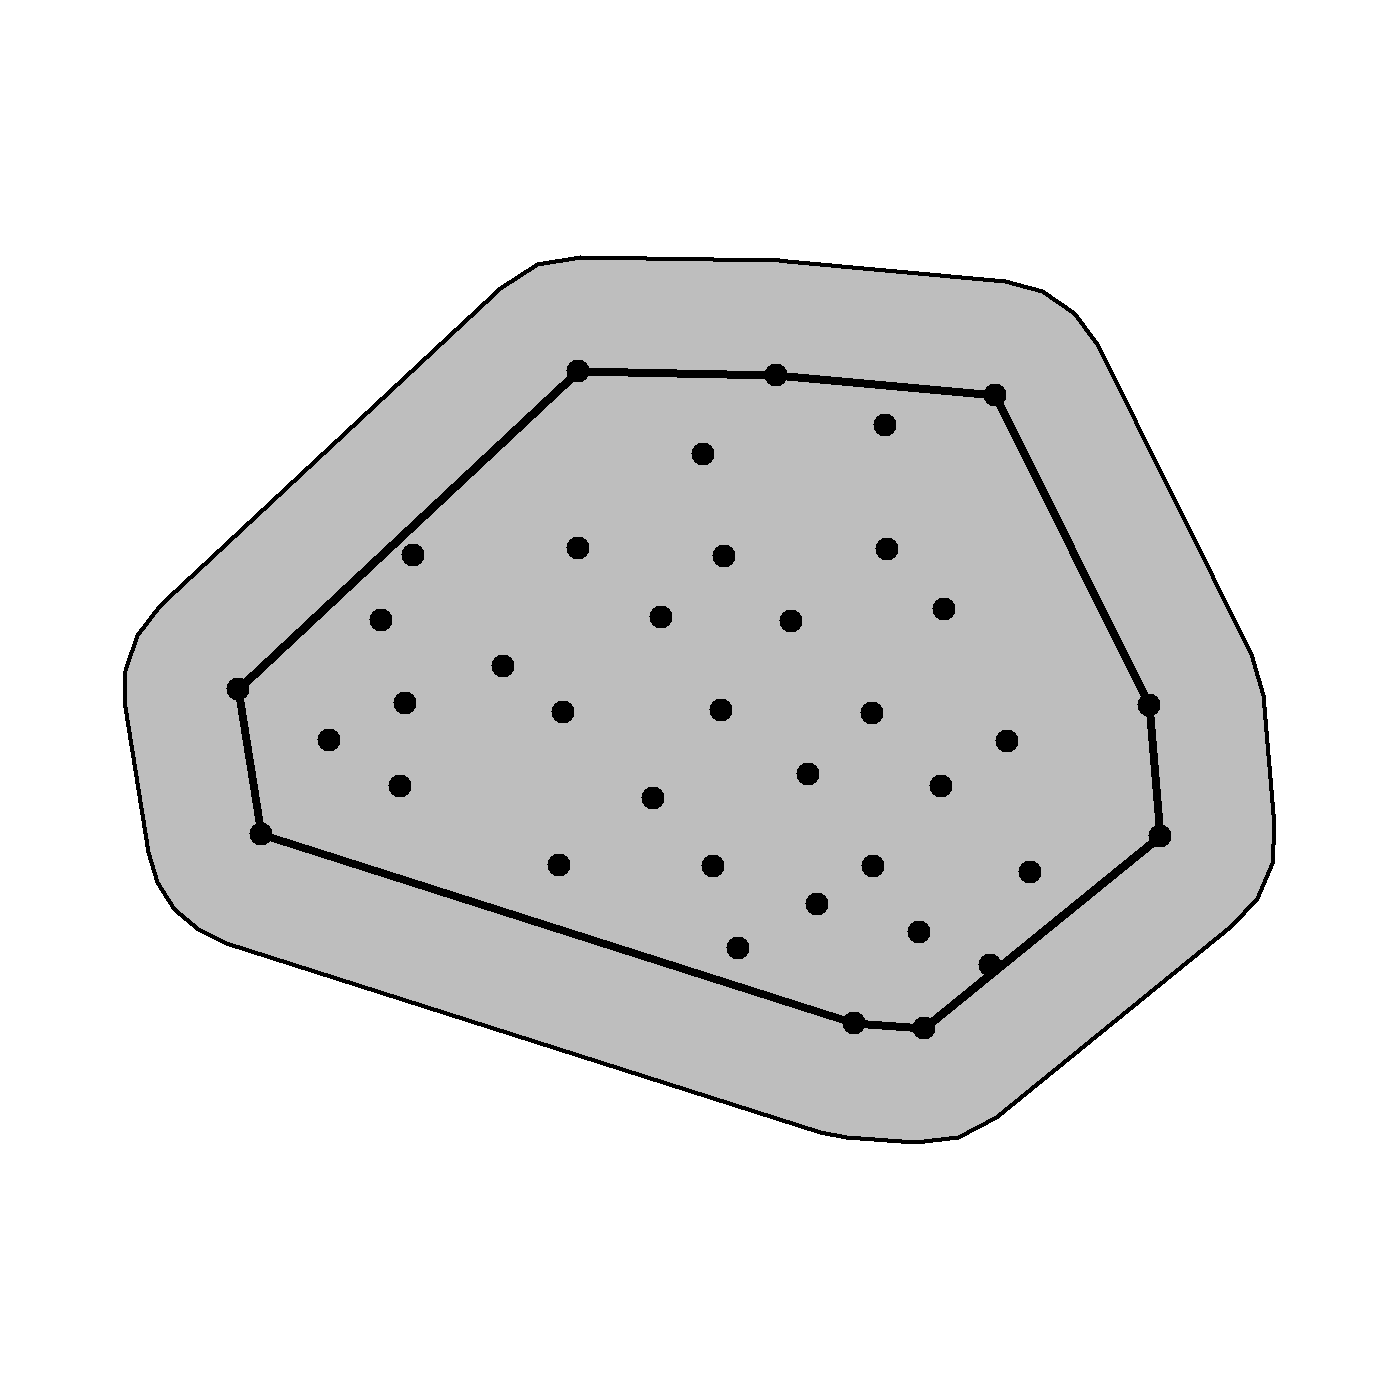
\includegraphics[height=3in,width=3in]{Ch4-Closed/figs/bufferedCH}
\end{center}
\caption{Convex hull of the bear hair snare array at Fort Drum, NY buffered by mean female
home range radius (2.19 km).}
\label{closed.fig.bch}
\end{figure}

To conjure up a
density estimate under model $M_0$, we compute the appropriate
posterior summary of the ratio of $N$ and the prescribed area ($277.011$ km$^2$):
{\small
\begin{verbatim}
> summary(fit0$sims.list$N/277.011)
   Min. 1st Qu.  Median    Mean 3rd Qu.    Max.
 0.1697  0.1733  0.1805  0.1803  0.1841  0.2130

> quantile(fit0$sims.list$N/277.011,c(0.025,0.975))
     2.5%     97.5%
0.1696684 0.1949381
\end{verbatim}
}
{\flushleft which } yields a density estimate of about $0.18$ ind/km$^2$, and a $95\%$ Bayesian
confidence interval of $(0.170, 0.195)$.

Our estimate of density should be reliable if we have faith in our
stated value of the ``sample area''. Clearly though this is largely
subjective, and not something we can formally evaluate (or estimate)
from the data based on model $M_{0}$.  More importantly, what exactly is the meaning of this
area -- in what quantitative sense is it the ``effective sample
area''? -- and, in this context, how do we gauge bias and/or variance
of ``estimators'' of it? These are questions that, to the best of our
knowledge, have not been addressed in any generality.
%\footnote{We note that \citet{karanth_nichols:1998} and
%  possibly others have computed
%  the variance of an estimated buffer strip, but do not provide a
%  quantitative definition of effective sample area.}.

\begin{comment}
How certain are we of this area? Can
we quantify our uncertainty about this quantity?
 More important, what exactly is
the meaning of this area and, in this context, how do we gauge bias
and/or variance of ``estimators'' of it? (i.e., what is it
estimating?).\footnote{Mention the delta approximation from
KARANTH AND NICHOLS (1998)?}
There is no theory to guide us in trying to answer these important questions.
\end{comment}

\section{Temporally varying and behavioral effects}
\label{closed.sec.timebehavefx}

The purpose of this chapter is mainly to emphasize the central
importance of the binomial model in capture-recapture and so we have
considered models for individual encounter frequencies---the number of
times individuals are captured out of $K$ occasions.  Sometimes we
can't aggregate the encounter data for each individual, such as when
encounter probability varies over time among samples.  Time-varying
responses that are relevant in many capture-recapture studies are
``effort'' such as amount of search time, number of observers, or trap
nights, or encounter probability varying over time, as a function of
date or season \citep{kery_etal:2010} due to species behavior.  A
common situation in many animal studies is that in which there exists
a ``behavioral response'' to trapping (even if the animal is not
physically trapped).
%For example, individuals might exhibit
%``trap happiness'' in response to baited traps. Conversely, individuals might learn
%to avoid traps (trap shyness) if the capture experience produces some negative
%stimulus.

Behavioral response is an important concept in animal studies
because individuals might learn to come to baited traps or avoid traps
due to trauma related to being encountered.  There are a number of
ways to parameterize a behavioral response to encounter. The
distinction between persistent and ephemeral was made by
\citet{yang_chao:2005} who considered a general behavioral response
model of the form:
\[
\mbox{logit}(p_{ik}) = \alpha_{0} + \alpha_{1} y_{i,k-1} + \alpha_{2} x_{ik}
\]
where $x_{ik}$ is a covariate indicator variable of previous capture
(i.e., $x_{ik} = 1$ if captured in any previous period). Therefore,
encounter probability changes depending on whether an individual was
captured in the immediate previous period (a Markovian or ephemeral behavioral
response; \citep{yang_chao:2005}), described by the term
$\alpha_{1} y_{i,k-1}$ or in {\it any} previous period (persistent behavioral
response), described by the term  $\alpha_{2} x_{ik}$.
%The former probably models a behavioral response due to
%individuals moving around their territory relatively slowly over time
%and the latter probably accommodates trap happiness due to baiting or
%shyness due to trauma.
Because spatial capture-recapture models allow us to include
trap-specific covariates, we can describe a 3rd type of behavioral
response---a local behavioral response that is trap-specific
\citep{royle_etal:2011jwm}. In this local behavioral response, the
encounter probability is modified for an individual trap depending on
previous capture in that trap.
Models with temporal effects are easy to describe and analyze in the {\bf BUGS} language
and we provide a number of examples in
Chapt. \ref{chapt.covariates} and elsewhere.


\section{ Models with individual heterogeneity}
\label{closed.sec.modelmh}

Models in which encounter probability varies by individual have a long
history in capture-recapture and, indeed, this so-called ``model
$M_h$'' is one of the elemental capture-recapture models in
\citep{otis_etal:1978}. Conceptually, we imagine that the
individual-specific encounter probability parameters, $p_{i}$, are
random variables distributed according to some probability
distribution, $[\theta]$. We denote this basic model assumption as
$p_{i} \sim [\theta]$. This type of model is similar in concept to
extending a GLM to a GLMM but in the capture-recapture context $N$ is
unknown.  The basic class of models is often referred to as ``model
$M_h$'' ('h' for heterogeneity), but really this is a broad class of
models, each being distinguished by the specific distribution assumed
for $p_{i}$.  There are many different varieties of model $M_{h}$
including parametric and various non-parametric approaches
\citep{burnham_overton:1978, norris_pollock:1996, pledger:2000}. One
important practical matter is that estimates of $N$ can be extremely
sensitive to the choice of heterogeneity model
\citep{fienberg_etal:1999, dorazio_royle:2003, link:2003}. Indeed,
\citet{link:2003} showed that in some cases it's possible to find
models that yield precisely the same expected data, yet produce wildly
different estimates of $N$. In that sense, $N$ for most practical
purposes is not identifiable across classes of different heterogeneity
models, and this should be understood before fitting any such
model. One solution to this problem is to seek to model explicit
factors that contribute to heterogeneity, e.g., using individual
covariate models (See \ref{closed.sec.indcov} below). Indeed, spatial
capture-recapture models seek to do just that, by modeling
heterogeneity due to the spatial organization of individuals in
relation to traps or other encounter mechanism.  For additional
background and applications of model $M_{h}$ see
\citet[][Chapt. 6]{royle_dorazio:2008} and
\citet[][Chapt. 6]{kery_schaub:2011}.

We will work with a specific type of model $M_{h}$ here which is a
natural extension of
the basic binomial observation model of model $M_{0}$ so
that
\[
\mbox{logit}(p_{i}) = \mu + \eta_{i}
\]
where $\mu$ is a fixed parameter (the mean) to be estimated, and
$\eta_{i}$ is an individual random effect assumed to be normally distributed:
\[
\eta_{i} \sim \mbox{Normal}(0, \sigma_{p}^2)
\]
We could as well combine these two steps and write $\mbox{logit}(p_{i}) \sim \mbox{Normal}(\mu,\sigma_{p}^2)$.
This ``logit-normal mixture'' was analyzed by
\citet{coull_agresti:1999} and elsewhere. It is a natural extension of
the basic model with constant $p$, as a mixed GLMM, and similar models
occur throughout statistics. It is also natural to consider a beta
prior distribution for $p_{i}$ \citep{dorazio_royle:2003} and
so-called ``finite-mixture'' models are also popular
\citep{norris_pollock:1996, pledger:2000}. In the latter, individuals
are assumed to belong to a finite number of latent classes, each of
which has its own capture probability.


Model $M_{h}$ has important historical relevance to spatial
capture-recapture situations \citep{karanth:1995} because
investigators recognized that the juxtaposition of individuals with
the array of trap locations should yield heterogeneity in encounter
probability, and thus it became common to use some version of model
$M_h$ in spatial trapping arrays to estimate $N$.  While this doesn't
resolve the problem of not knowing the effective sample area, 
it does yield an estimator that accommodates the heterogeneity in $p$
induced by the spatial aspect of capture-recapture studies.
To see how this juxtaposition induces heterogeneity, we have to
understand the relevance of movement in capture-recapture models.
Imagine a quadrat that can be uniformly searched by a crew of
biologists for some species of reptile (see \citet{royle_young:2008}).
Figure \ref{closed.fig.quadrat} shows a sample quadrat searched
repeatedly over a period of time. Further, suppose that the species
exhibits some sense of spatial fidelity in the form of a home range or
territory, and individuals move about their home range (home range
centroids are given by the blue dots) in some kind of random fashion.
%It is natural to think about it in terms of a
%movement process and sometimes that movement process can be modeled
%explicitly using hierarchical models \citep{royle_young:2008,
%  royle_etal:2011mee}.
Heuristically, we imagine that each individual in
the vicinity of the study area is liable to experience variable
exposure to encounter due to the overlap of its home range with the
sampled area - essentially the long-run proportion of times the
individual is within the sample plot boundaries, say $\phi$. We
might model the exposure or {\it availability} of an individual to 
capture by supposing that
$a_{i} = 1$ if individual $i$ is available to be captured (i.e.,
within the survey plot) during any sample, and $0$ otherwise. Then,
$\Pr(a_{i}=1) = \phi$.  In the context of spatial studies, it is
natural that $\phi$ should depend on {\it where} an individual lives,
i.e., it should be individual-specific $\phi_{i}$
\citep{chandler_etal:2011}. This system describes, precisely, that of
``random temporary emigration'' \citep{kendall_etal:1997} where $\phi_{i}$
is the individual-specific probability of being ``available'' for
capture.

Conceptually, SCR models aim to deal with
this problem of variable exposure to sampling due to movement in the
proximity of the trapping array explicitly and formally with auxiliary
spatial information.  If individuals are detected with probability
$p_{0}$, {\it conditional} on $a_{i} = 1$, then the marginal
probability of detecting  individual $i$ is
\[
 p_{i} = p_{0}\phi_{i}
\]
so we see clearly that individual heterogeneity in encounter
probability is induced as a result of the juxtaposition of individuals
(i.e., their home ranges) with the sample apparatus and the movement
of individuals about their home range.

\begin{figure}[ht]
\begin{center}
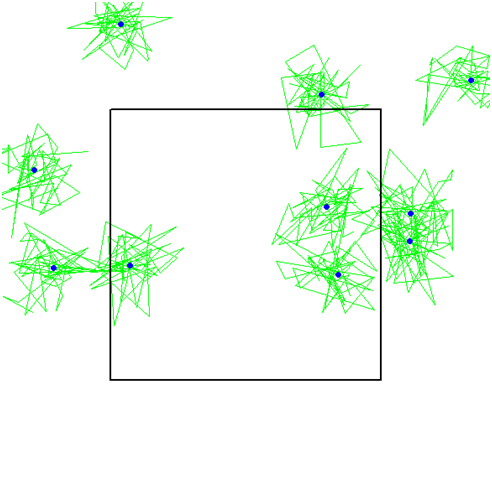
\includegraphics[height=3in]{Ch4-Closed/figs/quadrat}
\end{center}
\caption{A quadrat searched for lizards over some period of time
  (simulated data). The locations of encounter for each of 10 lizards are
  connected by lines---the dots are activity centers.}
\label{closed.fig.quadrat}
\end{figure}







\subsection{Analysis of Model $M_h$}

If $N$ is known, it is worth taking note of the essential simplicity
of model $M_h$ as a binomial GLMM.  This is a type of model that is
widely applied throughout statistics using
standard methods of inference based either on integrated likelihood
\citep{laird_ware:1982, berger_etal:1999}, which we discuss in
Chapt. \ref{chapt.mle}, or standard Bayesian
methods. However, because $N$ is not known, inference is somewhat more
challenging. We address that here using Bayesian analysis based on
data augmentation. Although we use data augmentation in the context of
Bayesian methods here, we note that
heterogeneity models formulated under DA are easily analyzed by
conventional likelihood methods as zero-inflated binomial mixtures
\citep{royle:2006} and more traditional analysis of model $M_h$ based on
integrated likelihood, without using data augmentation, has been
considered by \citet{coull_agresti:1999}, \citet{dorazio_royle:2003},
and others.

As with model $M_{0}$, we have the Bernoulli model for the
zero-inflation variables: $z_{i} \sim \mbox{Bern}(\psi)$ and the model
of the observations expressed conditional on these latent variables
$z_{i}$. For $z_{i}=1$, we have a binomial model with
individual-specific $p_{i}$:
\[
y_{i}|{z_{i} \! = \! 1} \sim \mbox{Binomial}(K,p_{i})
\]
and otherwise $y_{i} |{ z_{i} \! = \! 0} \sim 1(y=0)$, i.e., a point
mass at $y=0$ . Further, we
prescribe a distribution for $p_{i}$. Here we assume
\[
\mathrm{logit}(p_{i}) \sim \mbox{Normal}(\mu,\sigma^2)
\]
For prior distributions we assume
$p_{0} = \mbox{logit}^{-1}(\mu) \sim
\mbox{Uniform}(0,1)$ and, for the standard deviation
$\sigma \sim \mbox{Uniform}(0,B)$ for some large $B$.
\begin{comment}
The basic {\bf BUGS} description for this model is given as follows:
{\small
\begin{verbatim}
model{

p0 ~ dunif(0,1)       # prior distributions
mup<- log(p0/(1-p0))
sigmap ~ dunif(0,10)
taup<- 1/(sigmap*sigmap)
psi~dunif(0,1)

for(i in 1:(nind+nz)){
  z[i]~dbern(psi)     # zero inflation variables
  lp[i] ~ dnorm(mup,taup) # individual effect
  logit(p[i])<-lp[i]
  mu[i]<-z[i]*p[i]
  y[i]~dbin(mu[i],K)  #  observation model
 }

N<-sum(z[1:(nind+nz)])  # N is a derived parameter
}
\end{verbatim}
}
\end{comment}
Another common default prior is to assume
$\tau = 1/\sigma^{2} \sim \mbox{Gamma}(.1,.1)$, although we usually
choose  $\sigma \sim \mbox{Uniform}(0,B)$.



\subsection{Analysis of the Fort Drum data with model $M_{h}$}
\label{closed.sec.Mhbear}

Here we provide an analysis of the Fort Drum bear survey data using
the
 logit-normal heterogeneity model, and we
used data augmentation to produce a data
set of $M=700$ individuals.
%We note that
%the model runs effectively in {\bf WinBUGS} but sometimes with apparently
%inefficient mixing for reasons that may be related to bad starting
%values. In some cases this was resolved if we supplied starting values
%for the $\mbox{logit}(p_{i})$ parameters and $\tau$.
We have so far mostly used {\bf WinBUGS} but we are now transitioning
to the use of {\bf JAGS} run from within {\bf R} using the useful
packages \mbox{\tt R2jags} or \mbox{\tt rjags}.  The function
\mbox{\tt jags} from the \mbox{\tt R2jags} package runs essentially
like the \mbox{\tt bugs} function which we demonstrate here for
setting up and running model $M_{h}$ for the Fort Drum bear data:
{\small
\begin{verbatim}
[... get data as before ....]

set.seed(2013)

cat("
model{
p0 ~ dunif(0,1)       # prior distributions
mup<- log(p0/(1-p0))
sigmap ~ dunif(0,10)
taup<- 1/(sigmap*sigmap)
psi~dunif(0,1)

for(i in 1:(nind+nz)){
  z[i]~dbern(psi)     # zero inflation variables
  lp[i] ~ dnorm(mup,taup) # individual effect
  logit(p[i])<-lp[i]
  mu[i]<-z[i]*p[i]
  y[i]~dbin(mu[i],K)  #  observation model
 }

N<-sum(z[1:(nind+nz)])
}
",file="modelMh.txt")

data1 <- list(y=y, nz=nz, nind=nind,K=K)
params1 <- c('p0','sigmap','psi','N')
inits <- function() {list(z=as.numeric(y>=1), psi=.6, p0=runif(1),
          sigmap=runif(1,.7,1.2),lp=rnorm(M,-2)) }
library(R2jags)
wbout <- jags(data1, inits, params1, model.file = "modelMh.txt", n.chains = 3,
            n.iter = 1010000, n.burnin =10000, working.directory = getwd())
\end{verbatim}
}

We provide an {\bf R} function \mbox{\tt modelMhBUGS} in the package
\mbox{\tt scrbook} which will fit the model using either {\bf JAGS} or
{\bf WinBUGS} as specified by the user.  In addition, for fun, we
construct our own MCMC algorithm using a Metropolis-within-Gibbs
algorithm for model $M_{h}$ in Chapt. \ref{chapt.mcmc}, where we also
develop MCMC algorithms for spatial capture-recapture models.  Using
the {\bf WinBUGS} option in \mbox{\tt modelMhBUGS}, we ran 3 chains of 1
{\it million} iterations (mixing is poor for this model and this data
set), which produced the posterior distribution for $N$ shown in
Fig. \ref{closed.fig.bearMh}. Posterior summaries of parameters are
given in Table \ref{closed.tab.bear}.


\begin{table}[ht]
  \caption{
    Posterior summaries from model $M_h$ fitted to the Fort Drum black
    bear data. Results 
    were obtained using {\bf WinBUGS}
    running 3 chains, each with 1010000 iterations, discarding the
    first 10000 for a total of three {\it million} posterior samples. 
%\footnote{The reported \mbox{\tt n.sims} printed appears
%  to be an error in the \mbox{\tt R2WinBUGS} package}: 
}
\begin{tabular}{crrrrrrr} \hline \hline
 parameter &  mean   &  sd    &   2.5\% &  50 \%  &   97.5\% &Rhat& n.eff  \\ \hline
$p_0$      &   0.072 & 0.056  &   0.002 &  0.060  &   0.203  &1.008 &
540  \\ 
$\sigma_p$ &    2.096&  0.557 &   1.215 &  2.025  &   3.373  &1.003 &
820 \\ 
$\psi$     &    0.176&  0.101 &   0.084 &  0.147  &   0.458  & 1.006&
650 \\ 
$N$        & 122.695 &69.897  &  62.000 & 102.000 & 319.000  &1.006 &
630 \\ \hline
%deviance 187.089 17.998 155.400   185.900  225.700 1.002  3600
\end{tabular}
\label{closed.tab.bear}
\end{table}


We used $M=700$ for this analysis and we
note that  while the posterior mass of $N$ is concentrated away from this
upper bound (Fig. \ref{closed.fig.bearMh}), the posterior has an
extremely long right tail, with some MCMC draws at the upper
boundary $N=700$, suggesting that an even higher value of $M$ may be
called for.
%To make this plot and summarize the posterior distribution
%of model parameters, we have to grab the output from running {\bf
%  JAGS} in a slightly different manner -- the returned object is a
%list which contains {\bf R2WinBUGS}-like output in the list \mbox{\tt
%  BUGSoutput}. XXXX OBSOLETE? XXXXX
To characterize the posterior distribution of density we produce the
relevant summaries of the posterior distribution of $D  = N/277.11$
(recall
the buffered area of the convex hull is 277.11 $km^2$):
{\small
\begin{verbatim}
> summary(wbout$sims.list$N/277.11)
   Min. 1st Qu.  Median    Mean 3rd Qu.    Max.
 0.1696  0.2959  0.3681  0.4428  0.4944  2.5260

> quantile(wbout$sims.list$N/277.11,c(0.025,0.50,0.975))
     2.5%       50%     97.5%
0.2237379 0.3680849 1.1511674
\end{verbatim}
}
{\flushleft Therefore}, the point estimate, characterized by the posterior median, is around
$0.37$ bears per square km and a 95\% Bayesian credible interval is
$(0.224, 1.151)$.


\begin{figure}[ht]
\centering
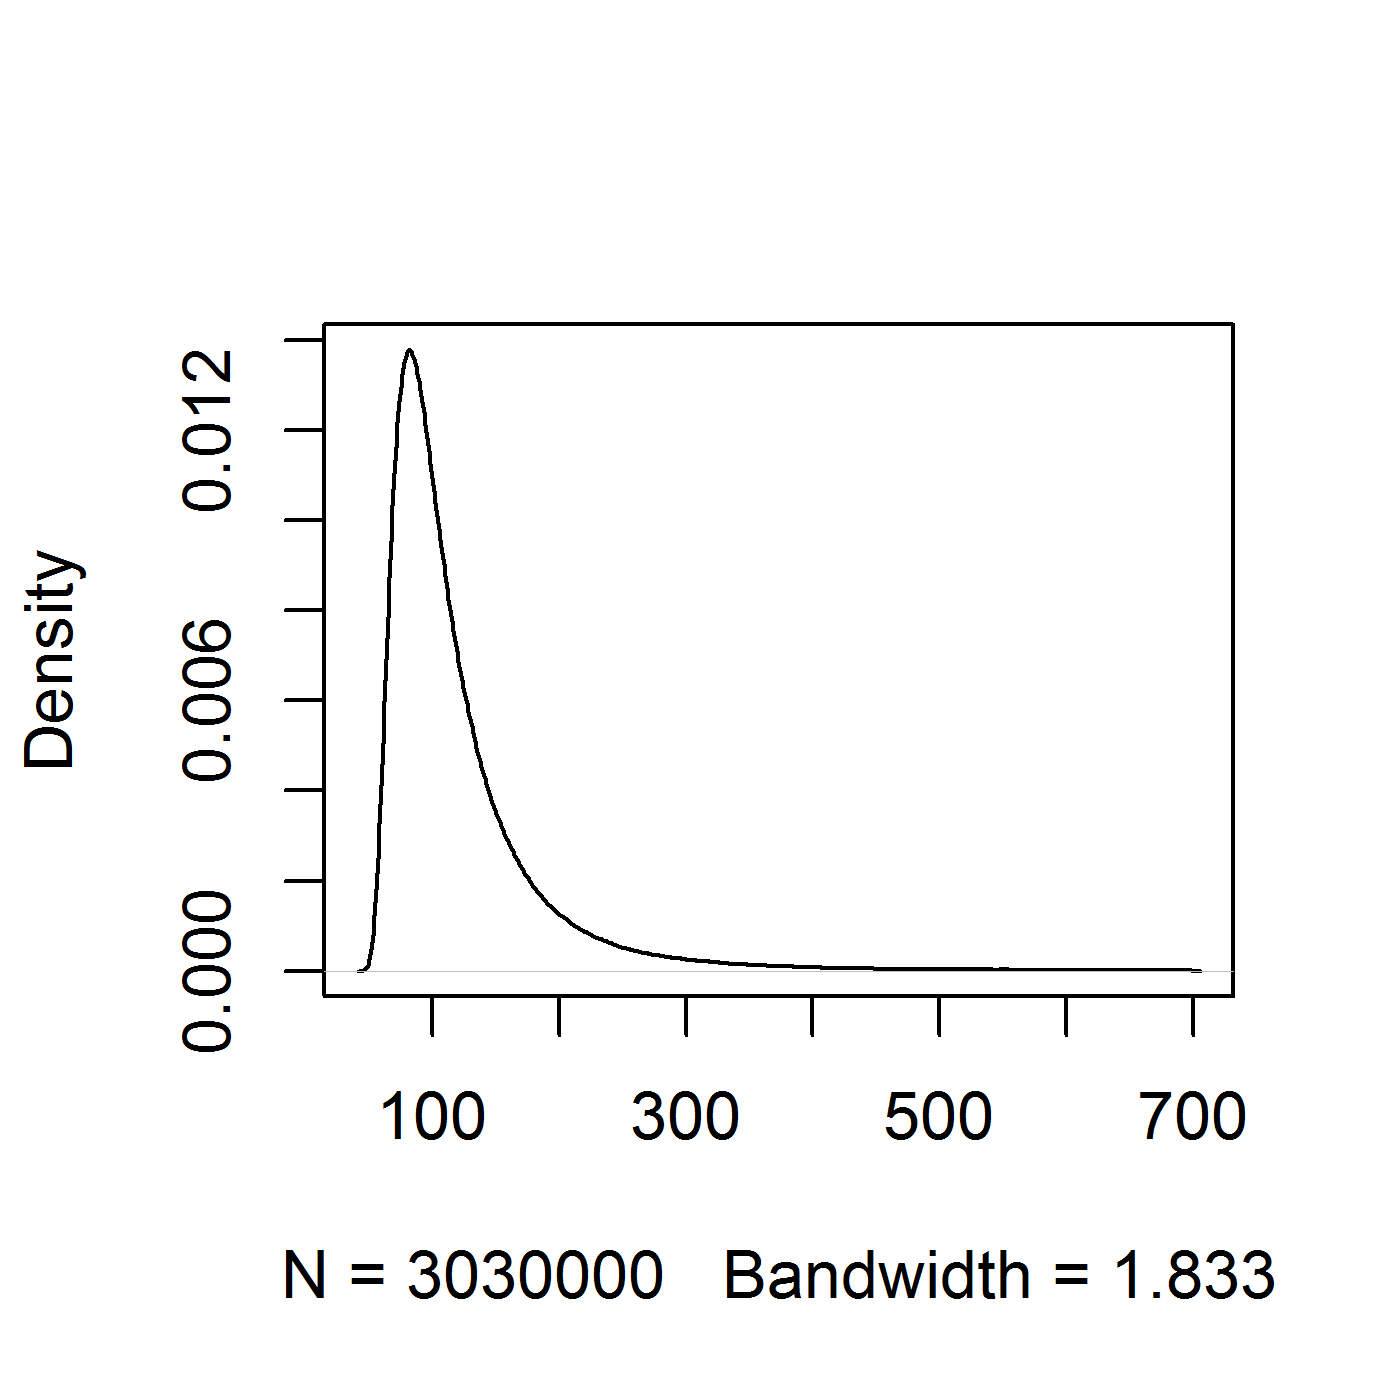
\includegraphics[height=3.5in,width=3.5in]{Ch4-Closed/figs/bear-modelMh-post-v2}
\caption{Posterior of $N$ for Fort Drum bear study data under the
logit-normal version of model $M_h$.
}
\label{closed.fig.bearMh}
\end{figure}

\subsection{Comparison with MLE}

The posterior of $N$ is highly skewed; therefore, we see that the
posterior mean
($N=122.7$) is considerably higher than the posterior median
($N=102$).
Further, it may be surprising that these posterior
summaries do not compare well with the MLE.
We used
the {\bf R} code contained in Panel 6.1 from
\citet{royle_dorazio:2008} to obtain the
MLE of $\log(n_{0})$, the logarithm of the number of uncaptured
individuals, is $\widehat{\log(n0)} = 3.86$ and therefore $\hat{N} =
\exp(3.86)+47 = 94.47$, much higher than the mode
shown in Fig. \ref{closed.fig.bearMh}.
To see this, we compute the posterior mode\index{posterior mode,
  calculation of} by finding
the posterior value of $N$ with the highest mass.
 Because $N$ is discrete, we can  use
the \mbox{\tt table()} function in {\bf R} and find the most frequent value
\footnote{For a continuous random variable we can use the function
 \mbox{\tt
    density()} to smooth the posterior samples and obtain the mode.}.
% Here are the
%commands for doing this:
%\begin{verbatim}
% N<-table(jout$BUGSoutput$sims.list$N)
% N[N==max(N)]
%   84
% 41961
%\end{verbatim}
If we want to smooth out some of the Monte
Carlo error a bit, we can use a smoother of some sort applied to the tabled
posterior frequencies of $N$. Here we use a smoothing spline ({\bf R}
function \mbox{\tt smooth.spline}) with the
degree of smoothing chosen by cross-validation (the \mbox{\tt cv=TRUE}
argument):
{\small
\begin{verbatim}
> N <- table(jout$BUGSoutput$sims.list$N)
> xg <- as.numeric(names(N))

> sp <- smooth.spline(xg,N,cv=TRUE)

> sp

Call:
smooth.spline(x = xg, y = N, cv = TRUE)

Smoothing Parameter  spar= 0.09339815  lambda= 8.201724e-09 (17 iterations)
Equivalent Degrees of Freedom (Df): 121.1825
Penalized Criterion: 2544481
PRESS: 5903.4
\end{verbatim}
}
We obtain the mode of the smoothed frequencies as follows:
\begin{verbatim}
sp$x[sp$y==max(sp$y)]
[1] 82
\end{verbatim}
%The \mbox{\tt df} argument controls the degree of smoothing and we can
%play around with that value or choose it using some method such as cross-validation
%find in this case that the modal value (i.e., 82) is not too sensitive
%to the smoothing parameter but this should be checked in any specific
%instance\footnote{we need to give examples of using \mbox{\tt
%    density()} to obtain modes}.


\begin{comment}
We note that any scalar summary of the posterior distribution is
pretty inconsistent with the MLE.
We used
the {\bf R} code contained in Panel 6.1 from
\citet{royle_dorazio:2008} to obtain the
MLE of $\log(n_{0})$, the logarithm of the number of uncaptured
individuals, is $\widehat{\log(n0)} = 3.86$ and therefore $\hat{N} =
\exp(3.86)+47 = 94.47$ which is considerably higher than the mode
shown in Fig. \ref{closed.fig.bearMh}.
%\footnote{We note that the result is inconsistent with Gardner et
%  al. (2009) who reported an MLE of 104.1 ($density = 0.437
%  inds/km^2$) although we do not know the reason for this at the
%  present time.}
%To convert this to density we use the buffered area
%as computed above (255.3 $km^2$)\footnote{WRONG \#} and perform the
%required summary analysis on the posterior samples of $N$, which
%results in about $0.37$ individuals/$km^2$. The reader should carry
%out this analysis to confirm the estimates, and also obtain the $95\%$
%confidence interval.
\end{comment}


We don't dwell too much on the difference between the MLE and features
of the posterior, 
 but we do note here that
the posterior distribution for the parameters of this model, for the
Fort Drum data set, are very sensitive to the prior
distributions. While MLEs are invariant to transformation of the
parameters, the posterior distribution definitely is {\it not}
invariant. In the present case, the use of a $\mbox{Uniform}(0,1)$
prior for $p_{0} = \mbox{logit}^{-1}(\mu)$ is somewhat
informative---in particular, it is not at all ``flat'' on the scale of
$\mu$, and this affects the posterior.  We generally always recommend
use of a $\mbox{Uniform}(0,1)$ prior for $\mbox{logit}^{-1}(\mu)$ in
such models. That said, we were surprised at this result, and we
experimented with other prior configurations including putting a flat
prior on $\mu$ directly. 
%That specific prior suggests the possibility
%that the posterior distribution may be improper for that prior
%specification. 
This kind of small sample instability has been widely
noted in model $M_h$ \citep{fienberg_etal:1999, dorazio_royle:2003},
as has extreme sensitivity to the specific form of model $M_{h}$
\citep{link:2003}.  In summary, while the mode is well-defined, the
data set is relatively sparse and hence inferences are poor and
sensitive to model choice.






\begin{comment}

\subsection{Exercises related to model $M_h$}

\begin{itemize}
\item[(1)] Enclose the MCMC algorithm in an R function and provide
  arguments for some of the parameters of the function that a user
  might wish to modify.
\item[(2)] Execute the function and compare the results to those
  generated from WinBUGS in the previous section
\item[(3)] Note that the prior distribution for the ``mean'' parameter
  is given on $p_0=\exp(\mu)/(1+exp(\mu))$.  Reformulate the algorithm
  with a flat prior on $\mu$ and see what happens. Contemplate this.
\item[(4)] Using Bayes rule, figure out the full conditional for
  $z_{i}$ so that you don't have to use MH for that one. It might be
  more efficient. Is it?
\item[(5)] Modify the MCMC algorithm so that the prior for $\mu_{p}$
  is an improper flat prior. i.e., $[\mu_{p}] \propto 1$. Describe the
  posterior distribution of $N$.
\end{itemize}

\end{comment}



\section{Individual Covariate Models: Toward Spatial Capture-Recapture}
\label{closed.sec.indcov}


A standard situation in capture-recapture models is when a covariate
which is thought to influence encounter probability is measured for
each individual. These are often called ``individual covariate
models'' but, in keeping with 
the classical nomenclature on closed
population models, \citet{kery_schaub:2011} 
referred to this class of models as ``model $M_{x}$'' (the $x$ here
being an explicit covariate).
 As with other closed population models, we begin
with the basic binomial observation model:
\[
y_{i} \sim \mbox{Binomial}(K, p_{i}).
\]
To model the covariate, we use a logit model for encounter probability
of the form:
\begin{equation}
 \mbox{logit}(p_{i}) = \alpha_0 + \alpha_1 x_{i}
\label{closed.eq.ha}
\end{equation}
where $x_i$ is the covariate value for individual $i$ and the
parameters $\bm{\alpha}= (\alpha_0, \alpha_1)$ are the regression coefficients. Classical
examples of covariates influencing detection probability are type of
animal (juvenile/adult or male/female), a continuous covariate such as
body mass \citep[e.g.,][Chapt. 6]{royle_dorazio:2008}, or a discrete covariate
such as group or cluster size. For example, in models of aerial survey
data, it is natural to model the detection probability of a group as a
function of the observation-level individual covariate, ``group size''
\citep{royle:2008, royle:2009, langtimm_etal:2011}.

Model $M_{x}$ is similar in structure to model
$M_{h}$, except that the individual effects are {\it observed} for the
$n$ individuals that appear in the sample. These models are important
here because spatial capture-recapture models can be described
precisely as a form of model $M_{x}$, where the covariate
describes {\it where} the individual is located in relation to the
trapping array.  Specifically, SCR models {\it are} individual
covariate models, but where the
individual covariate is only observed imperfectly (or partially
observed) for each 
captured individual.  Unlike model $M_h$, in model $M_{x}$
 (and SCR models) we do have some direct information about the
latent variable, which comes from the spatial locations/distribution
of individual recaptures.

Traditionally, estimation of $N$ in model $M_{x}$ is
achieved using methods based on ideas of unequal probability sampling
(i.e., Horvitz-Thompson estimation\footnote{For a  quick summary of
  the idea see: \\
  \url{http://en.wikipedia.org/wiki/Horvitz-Thompson_estimator}};
\citet{huggins:1989},
\citet{alho:1990} and \citet{borchers_etal:2002}). An estimator of $N$ is
\[
\hat{N} = \sum_{i=1}^{n} \frac{1}{\tilde{p}_{i}}
\]
where $\tilde{p}_{i}$ is the probability that individual $i$ appeared
in the sample.  That is, $\tilde{p}_{i} = \Pr(y_{i}>0)$
where, in closed population capture-recapture models,
\[
\Pr(y_{i}>0) = 1- (1-p_{i})^K
\]
where $p_{i}$ is a function of parameters $\alpha_{0}$ and $\alpha_{1}$
according to Eq. \ref{closed.eq.ha}.  In practice, parameters are
estimated from the conditional-likelihood of the observed encounter
histories which is, for observation $y_{i}$,
\begin{equation}
{\cal L}_{c}( {\bm \alpha} | y_{i}) = \frac{ \mbox{Binomial}(y_{i}|{\bm \alpha}) } { \tilde{p}_{i}}.
\label{closed.eq.cond}
\end{equation}
This derives from a straightforward application of the law of total
probability. Conceptually, we partition $\Pr(y)$ according to
$\Pr(y) = \Pr(y|y>0)\Pr(y>0) + \Pr(y|y=0)\Pr(y=0)$. For any positive
value of $y$ the 2nd term is necessarily 0, and so we rearrange to
obtain
$\Pr(y|y>0) = \Pr(y)/\Pr(y>0)$ which, in the specific case where
$\Pr(y)$ is the
binomial probability mass function (pmf) produces Eq. \ref{closed.eq.cond}.


Here we take a formal model-based approach to Bayesian analysis of
such models based on the joint likelihood using data augmentation
\citep{royle:2009}. Classical likelihood analysis of the so-called
``full likelihood'' is covered by \citet{borchers_etal:2002}.  For
Bayesian analysis of model $M_{x}$, because the 
individual covariate is unobserved for the $n_{0} = N-n$ uncaptured
individuals, we require a model to describe variation among
individuals, essentially allowing the sample to be extrapolated to the
population.  For example, if we have a continuous trait measured on
each individual, then we might assume that $x$ has a normal distribution:
\[
x_{i} \sim \mbox{Normal}(\mu,\sigma^{2})
\]
Data augmentation can be applied directly to this class of models. In
particular, reformulation of the model under DA yields a basic
zero-inflated binomial model of the following form, for each
$i=1,2,\ldots, M$:
\begin{eqnarray*}
z_{i} &\sim& \mbox{Bernoulli}(\psi)  \\
y_{i}|{z_{i}\! =\! 1} &\sim& \mbox{Binomial}(K,p_{i}(x_{i})) \\
y_{i} |{ z_{i}\! =\! 0} &\sim& 1(y=0)  \\
x_{i} & \sim & \mbox{Normal}(\mu,\sigma^{2})
\end{eqnarray*}
Fully spatial capture-recapture models use this formulation with a
latent covariate that is directly related to the individual detection
probability (see next section). As with the previous models,
implementation is trivial in the {\bf BUGS} language. The {\bf BUGS}
specification is very similar to that for model $M_h$, but we require
the distribution of the covariate to be specified, along with priors
for the parameters of that distribution.


\subsection{Example: Location of capture as a covariate.}

Here we consider a special type of model $M_{x}$ that is
especially relevant to spatial capture-recapture.  Intuitively, some
measure of distance from home range center to traps for an individual
should be a reasonable covariate to explain heterogeneity in encounter
probability, i.e., individuals with more exposure to traps should have
higher encounter probabilities and vice versa. So we can imagine {\it
  estimating} such a quantity, say average distance from home range
center to ``the trap array'', and then using it as an individual
covariate in capture-recapture models.  A version of this idea was put
forth by \citet{boulanger_mclellan:2001} (see also \citet{ivan:2012}),
but using the Huggins-Alho estimator and with covariate ``distance
from home range center to edge'' of the trapping array, where the home
range center is estimated by the average capture location.  This is
intuitively appealing because we can imagine, in some kind of an ideal
situation where we have a dense grid of traps over some geographic
region, that the average location of capture would be a decent
estimate (heuristically) of an individual's home range center.  We
provide an example of this type of approach
using a fully model-based analysis of the version of model $M_{x}$  
 described above, 
analyzed by data augmentation. We take a slightly different approach
than that adopted by \citet{boulanger_mclellan:2001}. By analyzing the
full likelihood and placing a prior distribution on the individual
covariate, we will resolve the problem of having an ill-defined
sample area.  After you read later chapters of this book, it will be
apparent that SCR models represent a formalization of this heuristic
procedure.


% A practical limitation of using sample estimates of individual covariates such
% as this is that it induces other statistical problems. Namely,
%it does not readily accommodate the
%inherent and heterogeneous variation of the  measured covariate, nor
%does it  provide a solution to the problem that the trap area
%is not well-defined.


For our purposes here, we define the individual covariate $x_{i} =
||{\bf s}_{i} - {\bf x}_{0}||$ where ${\bf s}_{i}$ is the average
encounter location of individual $i$ and ${\bf x}_{0}$ is the centroid
of the trap array.  In practice, people have used distance from edge
of the trap array but that is less easy to quantify, as ``edge''
itself is not precisely defined.  Conceptually, individuals in the
middle of the array should have a higher probability of encounter and,
as $x_{i}$ increases, $p_{i}$ should therefore decrease. We note that
we have defined ${\bf s}_{i}$ in terms of a sample quantity---the
observed mean encounter location---which, while ad hoc, is consistent
with the use of individual covariate models in the literature.  For an
expansive, dense trapping grid we might expect the sample mean
encounter location to be a good estimate of home range center but,
clearly this is biased for individuals that live around the edge (or
off) the trapping array.


A key point is that ${\bf s}_{i}$ is missing for each individual that
is not encountered and so $x_{i}$ is also missing. Therefore, it is a
latent variable, and we need to specify a probability distribution for
it.  As a measurement of distance we know it must be positive-valued,
and it seems sensible that an individual located extremely far from
the array of traps would not be captured.  Therefore, let's assume
that $x_{i}$ is uniformly distributed from $0$ to some large number,
say $B$, beyond which it would be difficult to imagine an individual
being captured by the trap array:
\[
 x_{i} \sim \mbox{Uniform}(0,B)
\]
where $B$ is a specified constant, which we may choose to be
arbitrarily large.
For example, $B$ should be at least a home
range diameter past the furthest trap from the centroid of the array.


\subsection{Fort Drum Bear Study}


We have to do a little bit of data processing to fit this individual
covariate model to the Fort Drum data.  We need to compute the
individual covariate ${\bf x}_{i}$ (distance from the centroid of the
trapping array) using the {\bf R} function \mbox{\tt spiderplot}
provided in \mbox{\tt scrbook}. This function also produces the keen
plot shown in Fig. \ref{closed.fig.spiderplot} which we call a
``spider plot''.  The {\bf R} commands for obtaining the individual
covariate ``distance from trap centroid'' (the variable \mbox{\tt
  xcent} returned by \mbox{\tt spiderplot}) and making the spider plot
are as follows:
\begin{verbatim}
library(scrbook)
data(beardata)
toad <- spiderplot(beardata$bearArray,beardata$trapmat)
xcent <- toad$xcent
\end{verbatim}

\begin{figure}[ht]
\centering
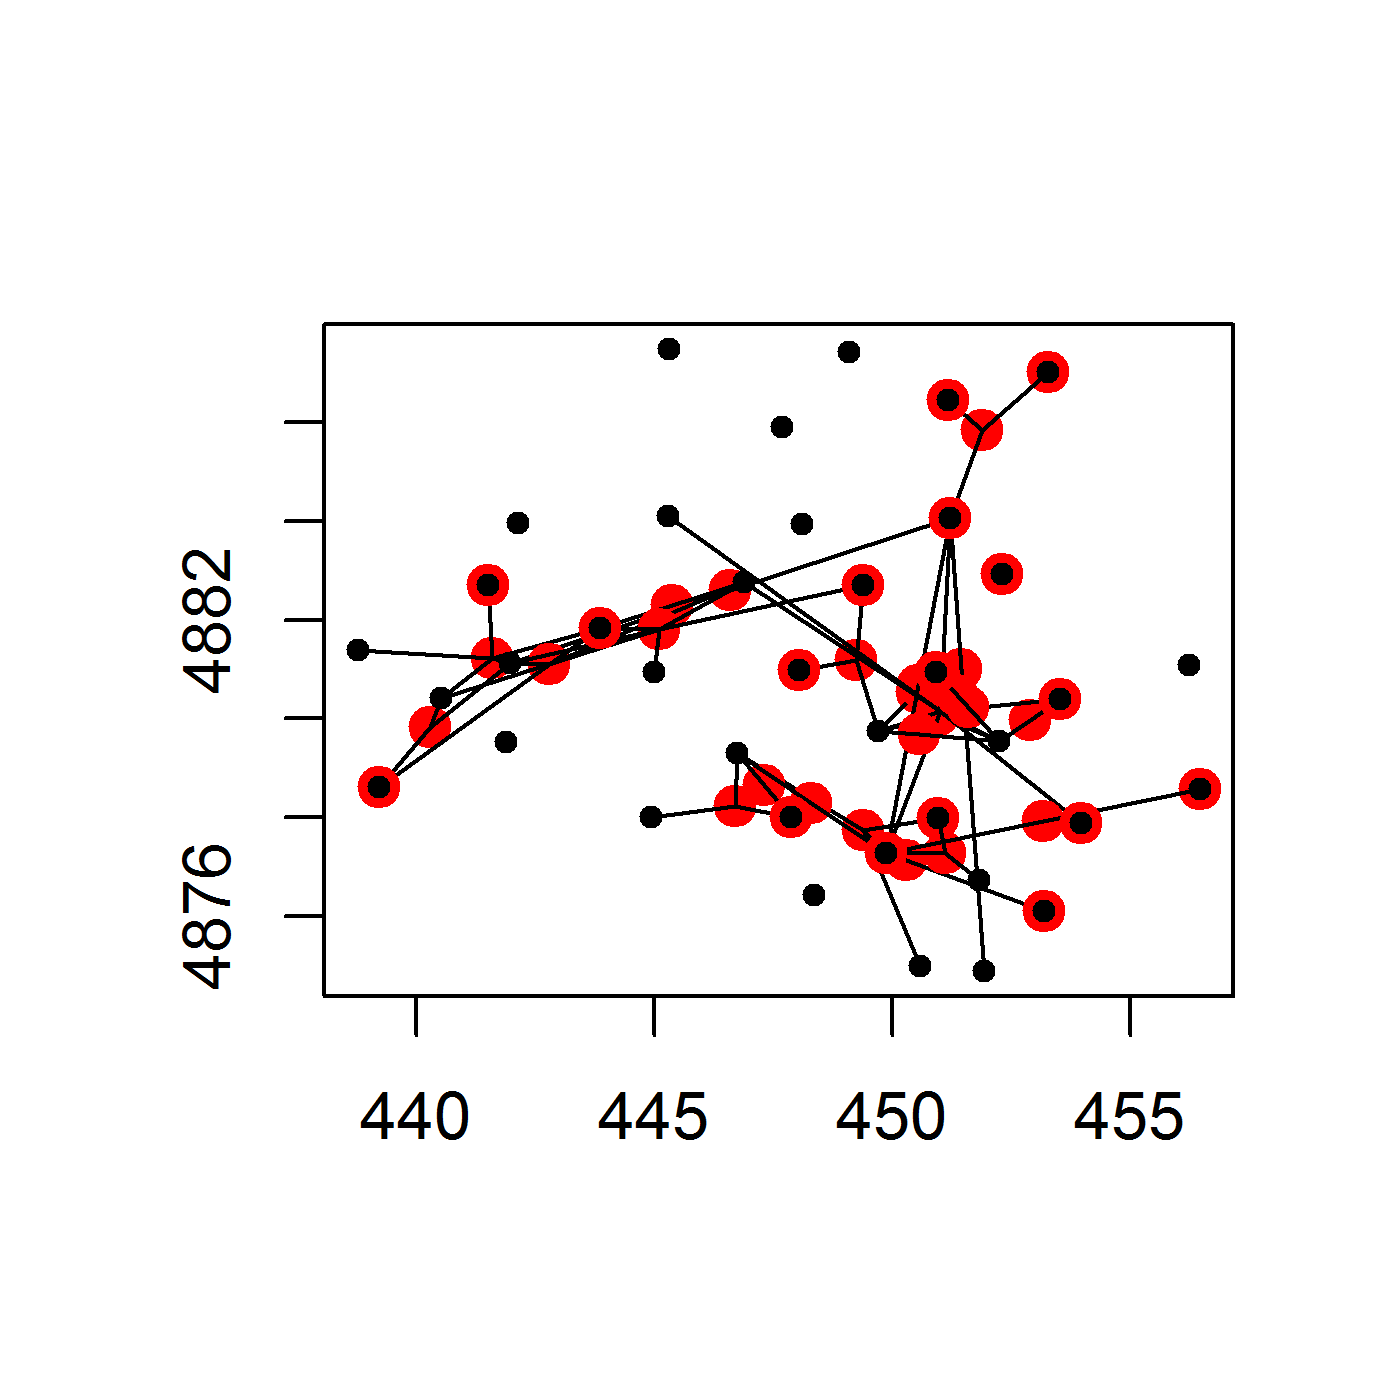
\includegraphics[height=3.5in,width=3.5in]{Ch4-Closed/figs/bear_spiderplot.png}
\caption{Spider plot of the Fort Drum study data.
The black dots represent the 47 trap locations with larger red dots
being the average capture location of each bear. i.e., its estimated home
range center. All traps in which a bear was captured are connected to
its estimated home range center with a line.
{\bf XXX note to Andy: change one of the dots to an X or something
  XXXXX }
}
\label{closed.fig.spiderplot}
\end{figure}

For the analysis of these data using the individual covariate
``distance from centroid'' we used $x_{i} \sim \mbox{Uniform}(0,B)$
with $B = 11.5$ $km^2$, which is about the distance from the array
center to the furthest trap.  Once we choose a value for $B$, the direct
implication is that the population size parameter, $N$, applies to the area
within 11.5 units of the trap centroid. Therefore, the model
associates a precise area within which the population of $N$ individuals
resides. 
We will see shortly that $N$
does, in fact, scale with our choice of $B$ to reflect the changing
area over which the $N$ individuals of the model reside.  The {\bf
  BUGS} model specification and {\bf R} commands to package the data
and fit the model are as follows:
{\small
\begin{verbatim}
cat("
model{
p0 ~ dunif(0,1)       # prior distributions
alpha0<- log(p0/(1-p0))
psi~dunif(0,1)
beta~dnorm(0,.01)

for(i in 1:(nind+nz)){
  xcent[i]~dunif(0,B)
  z[i]~dbern(psi)     # DA variables
  lp[i] <- alpha0 + beta*xcent[i] # individual effect
  logit(p[i])<-lp[i]
  mu[i]<-z[i]*p[i]
  y[i]~dbin(mu[i],K)  #  observation model
 }
N<-sum(z[1:(nind+nz)])
}
",file="modelMcov.txt")

data2 <- list(y=y,nz=nz,nind=nind,K=K,xcent=xcent,B=11.5)
params2 <- list('p0','psi','N','beta')
inits <- function() {list(z=zst, psi=psi, p0=runif(1),beta=rnorm(1) ) }
fit2 <-  bugs(data2, inits, params2, model.file="modelMcov.txt",
         n.chains=3, n.iter=11000, n.burnin=1000, n.thin=1)
\end{verbatim}
}
This produces the posterior summary statistics given in Table \ref{closed.tab.bear2}.

\begin{table}[ht]
  \caption{
    Posterior summaries from the individual covariate model (model
    $M_{x}$) with
    covariate ``distance from the centroid of the trap array'', 
 fitted to the Fort Drum black
    bear data. Results 
    were obtained using {\bf WinBUGS}
    running 3 chains, each with 11000 iterations, discarding the
    first 1000 for a total of 30000 posterior samples. 
}
\begin{tabular}{crrrrrrr} \hline \hline
 parameter &  mean&  sd  &   2.5\% &  50 \%  &   97.5\% &Rhat& n.eff  \\ \hline
p0         &0.54  &0.07  & 0.40   &  0.54  &  0.67  &  1 & 1100  \\
psi        &0.34  &0.05  & 0.25   &  0.34  &  0.44  &  1 & 3500 \\
N          &58.92 & 5.49 & 50.00  &  58.00 &  71.00 &   1&  1900 \\
beta       &-0.25 & 0.06 & -0.36  &  -0.25 &  -0.12 &   1&   780 \\ \hline
%deviance 459.51 13.21 435.80  458.80  487.40    1  2600
\end{tabular}
\label{closed.tab.bear2}
\end{table}



We note that the estimated $N$ is much lower than obtained by model
$M_h$ but there is a good explanation for this which we discuss in the
next section.
That issue notwithstanding, it is worth pondering how
this model could be an improvement (conceptually or technically) over
some other model/estimator including $M_0$ and $M_h$ considered
previously. Well, for one, we have accounted formally for
heterogeneity due to spatial location of individuals relative to
exposure to the trap array, characterized by the centroid of the
array. Moreover, we have done so using a model that is based on an
explicit mechanism, as opposed to a phenomenological one such as model
$M_h$. In addition, and importantly, using our new model, {\it the estimated
  N applies to an explicit area which is defined by our prescribed
  value of $B$}. That is, this area is a fixed component of the model
and the parameter $N$ therefore has explicit spatial context, as the
number of individuals with home range centers less than $B$ from the
centroid of the trap array. As such, the implied ``effective area'' of
the trap array for a given $B$ is a precisely defined quantity---it is
that of a circle with with radius $B$.


\subsection{Extension of the Model}

The model developed in the previous section is not a very good model
for one important reason: Imposing a uniform prior distribution on $x$
implies that density is {\it not constant} over space. In particular,
this model implies that density {\it decreases} as we move away from the
centroid of the trap array.  That is, $x_{i} \sim \mbox{Uniform}(0,B)$
implies constant $N$ in each distance band from the centroid but
obviously the {\it area} of each distance band is increasing.  This is
one reason we have a lower estimate of density than that obtained
previously from model $M_h$ (Sec. \ref{closed.sec.Mhbear}) and also
why, if we were to increase $B$, we would see density continue to
decrease.

Fortunately, we are not
restricted to use of this specific distribution for the individual
covariate. Clearly, it is a bad choice and, therefore, we should think
about whether we can choose a better distribution for $B$---one that
doesn't imply a decreasing density as distance from the centroid
increases.  Conceptually, what we want to do is impose a prior on
distance from the centroid, $x$, such that density is proportional to
the amount of area in each successive distance band as you move
farther away from the centroid.  In fact, theory exists which tells us
we should choose $[x] = 2x/B^2$. This can be derived
by noting that $F(x) = \Pr(X<x) = (\pi x^2)/(\pi*B^{2})$ . Then, $f(x)
= dF/dx = 2*x/(B^{2})$. This is a sort of triangular distribution in
density induced because the incremental area in each additional
distance band increases linearly with radius (i.e., distance from
centroid). This can be verified empirically as follows:
{\small
\begin{verbatim}
 u <- runif(10000,-1,1)
 v <- runif(10000,-1,1)
 d <- sqrt(u*u+v*v)
 hist(d[d<1])
 hist(d[d<1],100)
 hist(d[d<1],100,probability=TRUE)
 abline(0,2)
\end{verbatim}
}

It would be useful if we could describe this distribution directly in {\bf
  BUGS} but there is not a built-in way to do so. However, we can
implement a discrete version of the pdf\footnote{We might
also be able to use what is referred to in {\bf WinBUGS} jargon as the
``zeros trick'' (see {\it Advanced BUGS tricks} in the manual)
although we haven't pursued this approach.}. To do this,
we break $B$ into $L$
distance classes of width $\delta$, with probabilities proportional to
$2*x$. In particular, if we denote the cut-points by $g_{1}=0,g_{2},
\ldots, g_{L+1}=B$ and the interval midpoints are $m_{i} =
g_{i+1}-\delta$.
Then the interval probabilities are, approximately\footnote{This is
  just length $\times$ width, the area of small rectangles approximating the integral.}, $p_{i} =
\delta (2 m_{i} /B^{2})$, which we can compute once and then
pass them to {\bf BUGS} as data.
The {\bf R} commands for doing all of this (noting that we have
already loaded and processed the Fort Drum bear data) are given in the
following {\bf R}/{\bf BUGS} script:
% andy changed Dgrid to "midpts" and "Dmax" to "B" on 1/13/2013
% needs changed in repo!
{\small
\begin{verbatim}
delta <- .2
xbin <- xcent%/%delta  + 1               # put x in bins
midpts <- seq(delta,Dmax,delta)
xprobs <- delta*(2*midpts/(B*B))
xprobs <- xprobs/sum(xprobs)

cat("
model{
p0 ~ dunif(0,1)                        # prior distributions
alpha0<- log(p0/(1-p0))
psi~dunif(0,1)
beta~dnorm(0,.01)

for(i in 1:(nind+nz)){
  xbin[i]~dcat(xprobs[])
  z[i]~dbern(psi)                      # DA variables
  lp[i] <- alpha0 + beta*xbin[i]*delta # individual covariate model
  logit(p[i])<-lp[i]
  mu[i]<-z[i]*p[i]
  y[i]~dbin(mu[i],K)                   #  observation model
 }

N<-sum(z[1:(nind+nz)])                 # N is derived
}
",file="modelMcov.txt")
\end{verbatim}
}
In the model description the variable $x$ (observed distance
from centroid of the trap array) has been rounded or binned so that the discrete
version of the pdf of $x$ can be used as described previously. The new
variable labeled \mbox{\tt xbin} is then the {\it integer category}
in units of $\delta$ from 0. Thus, to convert back to distance in the
expression for \mbox{\tt lp[i]}, \mbox{\tt xbin[i]} has to be multiplied by
$\delta$.
To fit the model, keeping in mind that the data objects
required below have been defined in previous analyses of this chapter,
we do this:
{\small
\begin{verbatim}
data2 <- list(y=y,nz=nz,nind=nind,K=K,xbin=xbin,xprobs=xprobs,delta=delta)
params2 <- list('p0','psi','N','beta')
inits <- function() {list(z=z, psi=psi, p0=runif(1),beta=rnorm(1) ) }
fit <- bugs(data2, inits, params2, model.file="modelMcov.txt",
          working.directory=getwd(), debug=FALSE, n.chains=3, n.iter=11000,
          n.burnin=1000, n.thin=2)
\end{verbatim}
}

By specification of $B$,
this model
induces a clear definition of area
in which the population of $N$ individuals reside.
The parameter $N$ of the model is the
population size that applies to the particular value of $B$ and,
as such, we will see that $N$ scales with our choice of $B$.
This might be disconcerting to some---we can get whatever value of
$N$ we want by changing $B$!
Fortunately, we find empirically, that while $N$ is
highly sensitive to the prescribed value of $B$, density appears
invariant to $B$ as long as $B$ is sufficiently
large. We fit the model for a random of values of $B$ from $B=12$ (restricting
values of $x$ to be in close proximity to
the trap array) on up to 20. The results are given in Table
\ref{closed.tab.Dmax}.

\begin{table}[ht]
\centering
\caption{Analysis of Fort Drum bear hair snare data using the
  individual covariate model, for different values of $B$, the upper
  limit of the uniform distribution of `distance from centroid of the
  trap array'. ``Density'' is the posterior mean of density.}
\begin{tabular}{ccc}
\hline \hline
 $B$ & Density (post. mean) & Posterior SD \\ \hline
  12& 0.230 & 0.038 \\
  15& 0.244 &0.041 \\
  17& 0.249 &0.044 \\
  18& 0.249 &0.043\\
  19& 0.250 &0.043\\
  20& 0.250 &0.044 \\
\hline
\end{tabular}
\label{closed.tab.Dmax}
\end{table}


We see that the posterior mean and SD of density (individuals per
square km) appear insensitive to choice of $B$ once we reach about
$B=17$ or so.
The estimated density of
0.25 per km$^2$ is actually quite a bit lower than we reported using
model $M_h$ for which no relevant ``area'' quantity is explicit in the
model (and so we had to make it up).  Using MLEs of $N$ in conjunction with buffer strips (see Tab.
\ref{intro.tab.fdests}) our estimates were in the range of
$0.32-0.43$ and see Sec.  \ref{closed.sec.modelmh} above.  On the
other hand our estimate of $\hat{D} = 0.25$ here (based on the
posterior mean) is higher than that reported from model $M_0$ using
the buffered area ($\hat{D} = 0.18$). There is no basis really for comparing or
contrasting these various estimates.
In
particular, application of models $M_0$ and $M_h$ are distinctly {\it
  not} spatially explicit models---the area within which the
population resides is not defined under either model. There is
therefore no reason at all to think that the estimates produced under
either closed population model, based on a buffered ``trap area'', are
justifiable by any theory. In fact, we would get exactly the same
estimate of $N$ no matter what we declare the area to be. On the other
hand, the individual covariate model uses an explicit model for
 ``distance from centroid'' that is a reasonable and
standard null model---it posits, in the absence of direct information,
that individual home range centers are randomly distributed in space
and that probability of detection depends on the distance between home
range center and the centroid of the trap array. Under this definition
of the system, we see that density is invariant to the choice of area,
which seems like a desirable feature.


\subsection{Invariance of density to $B$}

Under model $M_{x}$, and also under models that we
consider in later chapters, a general property of the estimators is
that while $N$ increases with the prescribed area of the model
(defined by $B$ in this model),
 we expect that density estimators should be
invariant to this area. In the model used above, we note that
$\mbox{Area}(B) = \pi B^{2}$ and $\mathbb{E}(\mbox{N}(B)) = \lambda
\mbox{Area}(B)$ and thus $\mathbb{E}(\mbox{Density}(B)) = \lambda$,
i.e., constant. This should be interpreted as the {\it prior}
density. Absent data, then realizations under the model will have
density $\lambda$ regardless of what $B$ is prescribed to be.  As we
verified empirically above,  posterior summaries of density are also invariant to
$B$ as long as the prescribed area is sufficiently large.
%large enough so
%that the data no longer provide information about density (i.e., ``far
%away'').

\subsection{Toward Fully Spatial Capture-recapture Models}

While the use of an individual covariate model  resolves two important problems
inherent in almost all capture-recapture studies (induced
heterogeneity and absence of a precise relationship between $N$ and
area), is not ideal for all purposes because it does not make full use
of the spatial information in the data set, i.e., the trap locations
and the locations of each individual encounter, so that we cannot use
this model to model trap-specific effects (e.g., trap effort or type).
Moreover, we applied this model for ``data'' being the average
observed encounter location,
and equated that summary to the home range center ${\bf s}_{i}$. Intuitively, taking
the average encounter location as an estimate of home range center
makes sense but more so when the trapping grid is dense and expansive
relative to typical home range sizes which might not be reasonable in
practice.
Moreover, this approach also
ignored the variable precision with which each ${\bf s}_{i}$ is
estimated. Finally, it ignores that  estimates of ${\bf s}_{i}$
around the ``edge'' (however we define that) are biased because the
observations are truncated---we can only observe locations interior to
the array.

However, there is hope to extend this model in order to resolve
these remaining deficiencies.  In the next chapter we provide a further
extension of this individual covariate model that definitively
resolves the {\it ad hoc} nature of the approach we
took here. In that chapter we build a model in which ${\bf s}_{i}$ are
regarded as latent variables and the observation locations (i.e., trap
specific encounters) are linked to those latent variables with an
explicit model. We note that the model fitted previously could be
adapted easily to deal with ${\bf s}_{i}$ as a latent variable, simply
by adding a prior distribution for ${\bf s}_{i}$.  This is actually
easier, and less ad hoc in a number of respects, and you should try it out.



\section{Distance Sampling: A Primitive SCR Model}

Distance sampling is a class of methods for estimating animal density
from measurements of distance from an observer to individual animals
(or groups). The basic assumption is that detection probability is
 a function of distance.
Distance sampling is one of the most popular methods for estimating
animal abundance \citep{burnham_etal:1980, buckland_etal:2001,
  buckland_etal:2004book} because, unlike ordinary closed population models,
distance sampling provides explicit estimates of {\it density}.
 In terms of
methodological context, the distance sampling model is a special case
of a closed population model with an individual covariate. The
covariate in this case, $x$, is the distance between an
individual's location say ${\bf u}$ and the observation location or transect. In
fact, distance sampling is precisely an
individual-covariate model, except
that observations are made at only $K=1$ sampling occasion. Thus, in
that sense, distance sampling is a spatial capture-recapture model,
% XXXX I'm not sure the reader quite understands how it is a "spatial"
% model at this point
but without the ``recapture.''  Distance sampling  eliminates the need to
explicitly identify individuals (except they need to be {\it
  distinguished} from other individuals) repeatedly and so distance
sampling can be applied to unmarked populations.
This first and most basic spatial
capture-recapture model has been used routinely for decades and,
formally, it is a spatially-explicit model in the sense that it
describes, explicitly, the spatial organization of individual
locations (although this is not always stated explicitly) and, as a
result, somewhat general models of how individuals are distributed in
space can be specified \citep{hedley_etal:1999, royle_etal:2004,
  johnson_etal:2010, niemi_fernandez:2010, sillett_etal:2012}.
% XXXX The Johnson et al 2010 Ref is missing coauthors

As with other models we've encountered in this chapter, the distance sampling model, under data augmentation,
includes a set of $M$ zero-inflation variables $z_{i}$ and a
binomial observation model expressed conditional on $z$ (binomial for $z=1$, and
fixed zeros for $z=0$).  In distance sampling we pay for having only a
single sample occasion (i.e., $K=1$) by requiring constraints on the model of
detection probability, normally imposed as the assumption that
detection probability is $1.0$ when distance equals 0.  A standard
model for detection probability is the ``half-normal'' model:
\[
p_{i} = \exp(-\alpha_{1} x_{i}^{2})
\]
for $\alpha_{1} > 0$, 
where $x_i$ denotes the distance at which the $i$th
individual is detected relative to some reference location where
perfect detectability ($p=1$) is assumed. This encounter probability
model is more often written with
$\alpha_{1} =
1/2\sigma^{2}$.  If $K>1$ then an intercept in this model, say $\alpha_{0}$, is
identifiable and such models are usually called ``capture-recapture
distance sampling''\citep{alpizar_pollock:1996,borchers_etal:1998}.

As with previous examples, we require a distribution for the
individual covariate $x_{i}$. The customary choice is
\[
x_{i} \sim \mbox{Uniform}(0,B)
\]
wherein $B>0$ is a known constant, being the upper limit of data
recording by the observer (i.e., the point count radius, or transect
half-width). In practice, this is sometimes asserted to be infinity,
but in such cases the distance data are usually truncated.
% XXXX Could cut previous sentence b/c I think people do use B=inf
% fairly often
Specification of this distance sampling model in the {\bf BUGS}
language  is
shown in Panel \ref{closed.panel.distance}, taken from \citet{royle_dorazio:2008}.


\begin{panel}[ht]
\centering
\rule[0.15in]{\textwidth}{.03in}
\begin{minipage}{5in}
\begin{verbatim}
alpha1~dunif(0,10)
psi~dunif(0,1)

for(i in 1:(nind+nz)){
   z[i]~dbern(psi)             # DA variables
   x[i]~dunif(0,B)             # B=strip width
   p[i]<-exp(logp[i])          # Detection function
   logp[i]<-   - alpha1*(x[i]*x[i])
   mu[i]<-z[i]*p[i]
   y[i]~dbern(mu[i])           # Observation model 
 }

N<-sum(z[1:(nind+nz)])         # N is a derived parameter
D<- N/striparea                # D = N/total area of transects
\end{verbatim}
\end{minipage}
\rule[-0.15in]{\textwidth}{.03in}
\caption{Distance sampling model in {\bf BUGS} for a line transect situation, using a half-normal
detection function.}
\label{closed.panel.distance}
\end{panel}

As with the individual covariate model in the previous section, the
distance sampling model can be equivalently specified by putting a
prior distribution on individual {\it location} instead of distance
between individual and observation point (or transect).  Thus we can
write the general distance sampling model as
\[
p_{i} = h(||{\bf u}_{i} - {\bf x}_0||,\alpha_{1})
\]
along with
\[
 {\bf u}_{i} \sim \mbox{Uniform}({\cal S})
\]
where ${\bf x}_{0}$ is a fixed point (or line) and ${\bf u}_{i}$ is
the individual's location,  which is observed for the sample of $n$ individuals. In
practice it is easier to record distance instead of location.  Basic
math can be used to argue that if individuals have a uniform
distribution in space, then the distribution of Euclidean distance is
also uniform. In particular, if a transect of length $L$ is used and $x$
is distance to the transect then $F(x) = \Pr(X\le x) = L*x/L*B = x/B$ and
$f(x) = dF/dx = (1/B)$. For measurements of radial distance, we
provided the analogous argument in the
previous section.


The preceding paragraph makes it clear that distance sampling is a
special case of spatial capture-recapture models, such as those
derived from model $M_{x}$ of the previous section, where the
encounter probability is related directly to {\it distance}, which is
a reduced information summary of {\it location}, ${\bf u}$.  Some
intermediate forms of SCR/DS models can be described
\citep{royle_etal:2011mee}.  In the context of our general
characterization of SCR models
(Chapt. \ref{modeling.sec.characterization}), we suggested that every
SCR model can be described, conceptually, by a hierarchical model of
the form:
\[
 [y|{\bf u}][{\bf u}|{\bf s}][{\bf s}].
\]
Distance sampling ignores the part of the model pertaining to ${\bf
  s}$, and deals only with the model components for the observed
data  ${\bf u}$\footnote{Equivalently, we could also say that $[{\bf u}]$ in
  the distance sampling model is $[{\bf u}] = \int [{\bf u}|{\bf s}][{\bf s}]
  d{\bf s}$}. Thus, we are left with a hierarchical model of the form
\[
[y|{\bf u}][{\bf u}].
\]
In contrast, as we will see in the next chapters, many  SCR models
(Chapt. \ref{chapt.scr0}) ignore ${\bf u}$ and condition on ${\bf s}$,
which is not observed:
\[
[y|{\bf s}][{\bf s}]
\]
Since $[{\bf u}]$ and $[{\bf s}]$ are both assumed to be uniformly
distributed, these are equivalent models! The main differences have to
do with interpretation of model components and whether or not the
latent variables are observable (in distance sampling they are).

So why bother with SCR models when distance sampling yields density
estimates and accounts for spatial heterogeneity in detection? For
one, imagine trying to collect distance sampling data on species such
as jaguars or tigers!  Clearly, distance sampling requires that one
can collect large quantities of distance data, which is not always
possible. For tigers, it is much easier, efficient, and safer to
employ camera traps or tracking plates and then apply SCR
models. Furthermore, as we will see in Chapt.
\ref{chapt.search-encounter}, SCR models can use distance data,
allowing us to study distribution, movement, and density. Thus, SCR
models are more general and versatile than distance sampling models
(which clearly are a special case), and can accommodate data from
virtually all animal survey designs.

\subsection{Example: Sonoran Desert Tortoise Study}

We illustrate the application of distance sampling models using data
on the Sonoran desert tortoise ({\it Gopherus agassizii}), shown in
Fig. \ref{closed.fig.tortoise}, collected along transects
in southern Arizona (see \citet{zylstra_etal:2010} for
details). The data are from 120 square transects having four 250 m sides,
 although we ignore this detail in our analysis here and regard
them as 1 km transects, and we pooled the detection data from all
120 transects. The histogram of encounter distances from the 65
encountered individuals is
shown in Fig. \ref{closed.fig.tortoisehist}
\begin{figure}[ht]
\centering
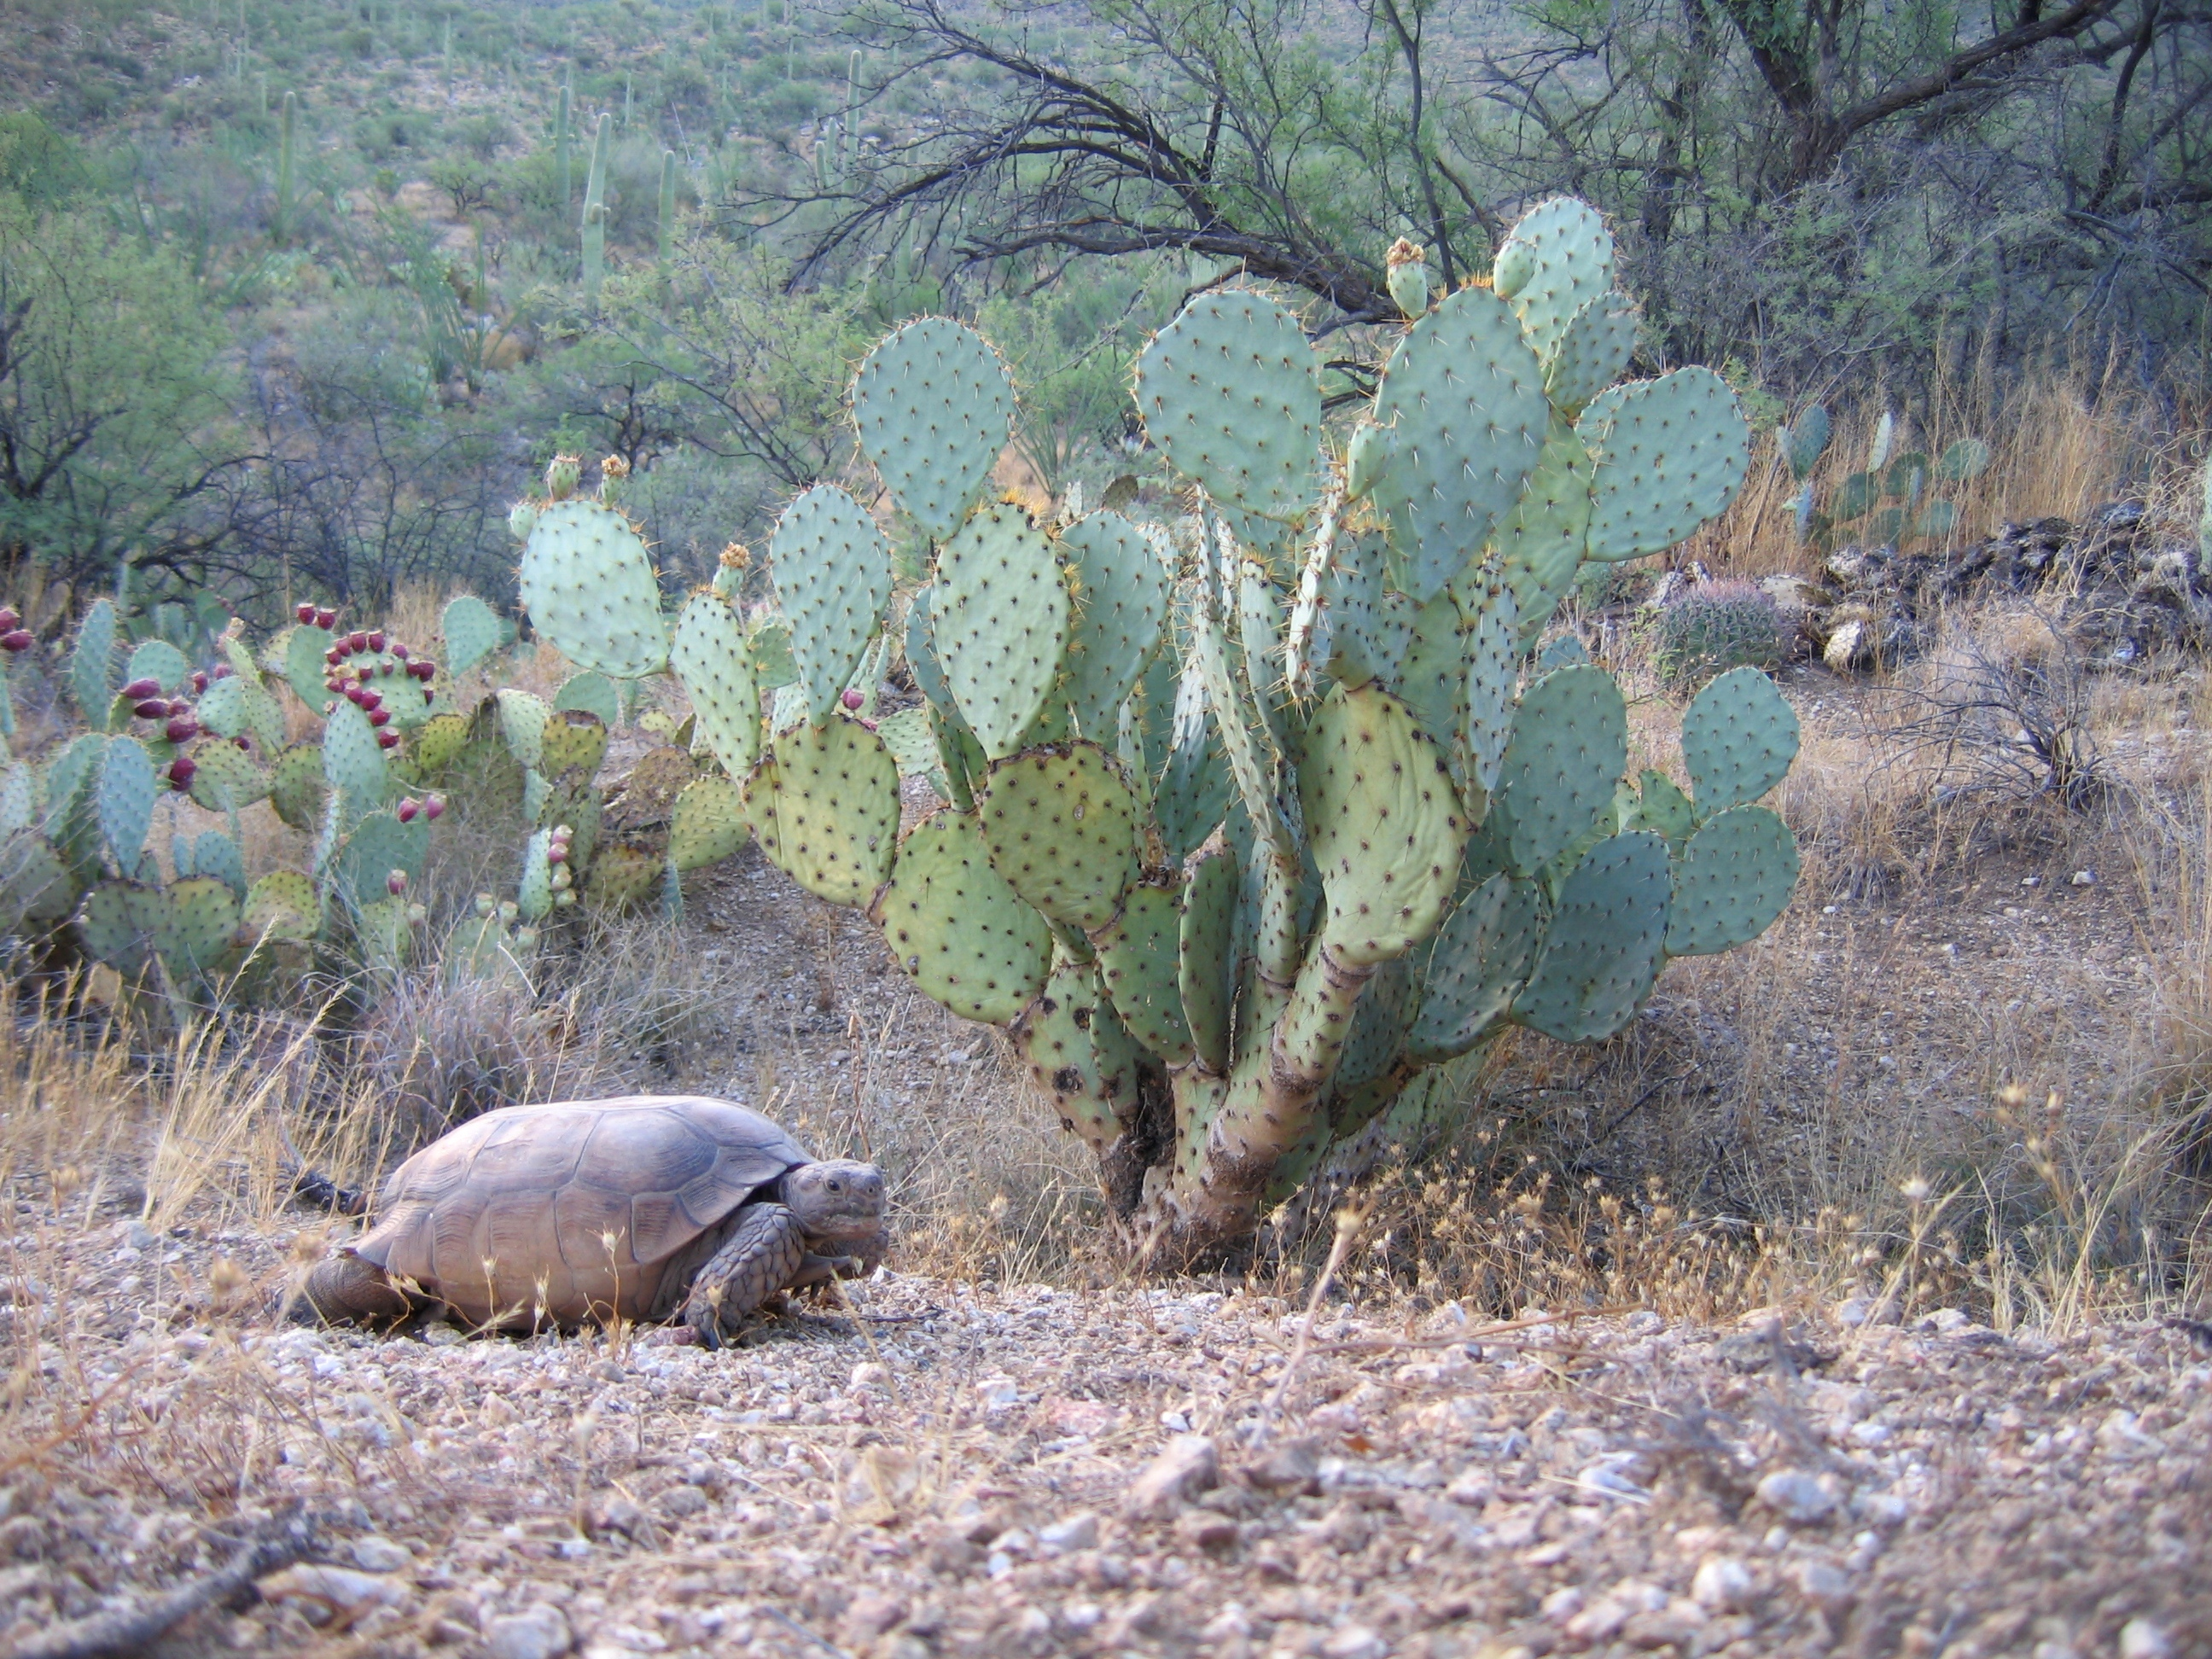
\includegraphics[height=3in,width=4in]{Ch4-Closed/figs/Erin_Zylstra_2.jpg}
\caption{Desert tortoise in its native habitat ({\it Photo credit: Erin
  Zylstra, Univ. of Arizona}).}
\label{closed.fig.tortoise}
\end{figure}

\begin{figure}[ht]
\centering
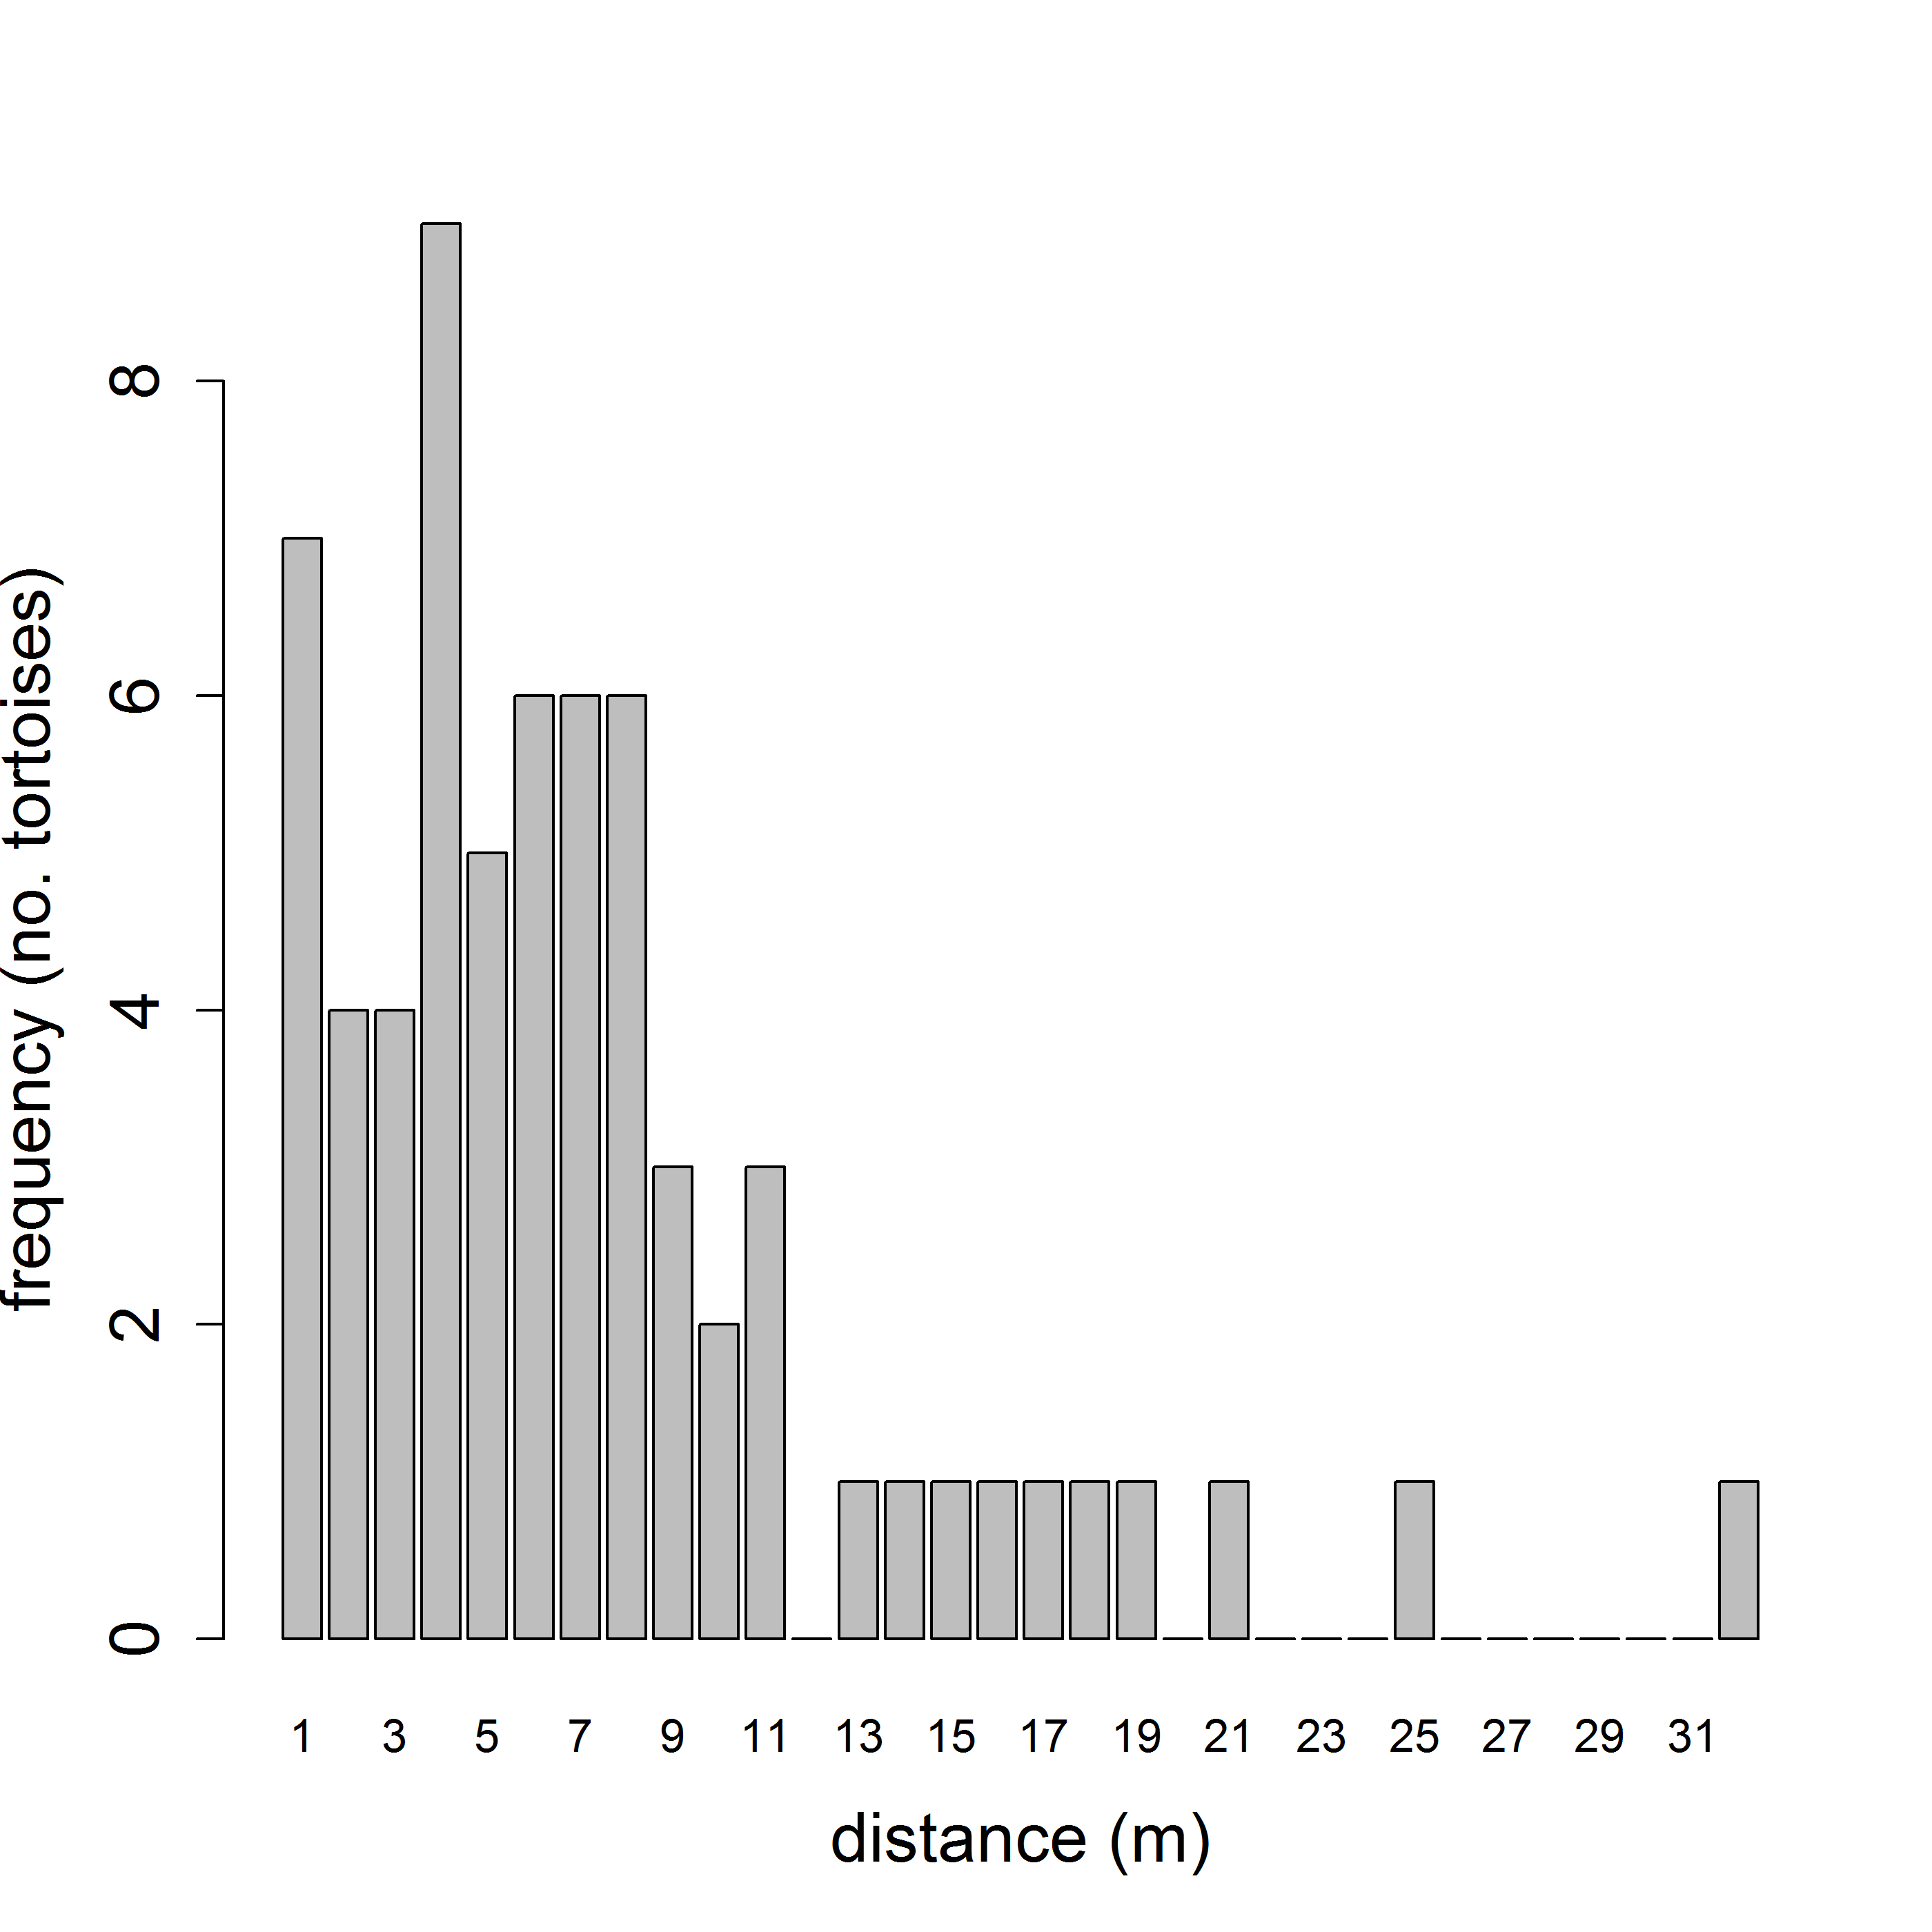
\includegraphics[height=2.8in,width=2.8in]{Ch4-Closed/figs/tortoise.png}
\caption{
Distance histogram of $n=65$ Sonoran desert tortoise detections from a
total of 120 km of
survey transect. }
\label{closed.fig.tortoisehist}
\end{figure}

Commands for reading in and organizing the data for analysis using {\bf
  WinBUGS} are given in the help file \mbox{\tt ?tortoise} provided
with the \mbox{\tt scrbook} package. 
To compute density, the total sampled area of the transects \mbox{\tt
  striparea} is input as data, and computed as: $120$ (transects)
multiplied by the length ($1000$ m) and half-width ($B=40$ m), then
multiplied by 2, and  divided by $10000$ to convert to
units of individuals per ha. 
We also provide commands for 
analyzing the data with \mbox{\tt unmarked}
\citep{fiske_chandler:2011} using hierarchical distance sampling
models \citep{royle_etal:2004}.

\begin{comment}
The full script is provided with the
\mbox{\tt scrbook} {\bf R} package (see \mbox{\tt ?tortoise}), where  
we also give some commands for
analyzing the data with \mbox{\tt unmarked}
\citep{fiske_chandler:2011} using hierarchical distance sampling
models \citep{royle_etal:2004}.
{\small
\begin{verbatim}
data(toroise)
x<-tortoise[,"Dist"]
nind<-sum(!is.na(x))

y<-rep(1,nind)        # create encounter vector
nz<-700               # data augmentation
y<-c(y,rep(0,nz))     # add 0s to the encounter vector
x<-c(x,rep(NA,nz))    # pad distance vector with NA
z<-y                  # starting vals for data augmentation variables

cat("
model{
alpha1~dunif(0,10)
sigma<- sqrt(1/(2*alpha1))
psi~dunif(0,1)

for(i in 1:(nind+nz)){
   z[i]~dbern(psi)      # DA Variables
   x[i]~dunif(0,B)      # B=strip width
   p[i]<-exp(logp[i])   # DETECTION MODEL
   logp[i]<-   -alpha1*(x[i]*x[i])
   mu[i]<-z[i]*p[i]
   y[i]~dbern(mu[i])    # OBSERVATION MODEL
 }

N<-sum(z[1:(nind+nz)])
D<- N/striparea  # area of transects
}
",file="dsamp.txt")
\end{verbatim}
}
After creating the model file, next
we bundle the data,
provide initial values, indicate which parameters to monitor, and then
pass those things to {\bf WinBUGS}:
{\small
\begin{verbatim}
library(R2WinBUGS)

# density to be reported in units of ind/ha
data<-list(y=y,x=x,nz=nz,nind=nind,B=40,striparea=(120*1000*40*2/10000))
params<-list('alpha1','sigma','N','D','psi')
inits =  function() {list(z=z, psi=runif(1), alpha1=runif(1,0,.02) )}
fit = bugs(data, inits, params, model.file="dsamp.txt",working.directory=getwd(),
       debug=FALSE, n.chains=3, n.iter=3000, n.burnin=1000, n.thin=2)
\end{verbatim}
}
\end{comment}

Posterior summaries for the tortoise data are given in Tab. \ref{closed.tab.dsamp}.
Estimated density (posterior mean) is $0.54$ individuals
  per ha and the estimated scale parameter of the distance function
(posterior mean) is $\sigma=9.12$ meters.  The Rhat statistics of
around $1.02$ suggest that slightly longer MCMC simulations might be
called for. The posterior mass of the data augmentation parameter $\psi$
is located away from the upper-bound $\psi=1$ and so the degree of
data augmentation appears sufficient.

\begin{table}[ht]
  \caption{
    Posterior summaries from the tortoise distance sampling data. Results
    were obtained using {\bf WinBUGS}
    running
    3 chains, each with 3000 iterations and the first 1000 discarded,
    thinning by 2.
  }
\begin{tabular}{crrrrrrr} \hline \hline
 parameter &mean &   sd  & 2.5\%   &  50 \%  &   97.5\% &Rhat& n.eff
 \\ \hline
$\alpha_1$ &  0.01&  0.00 &   0.00 &  0.01   &   0.01 &1.02&   130   \\
$\sigma$  &   9.12&  0.77 &   7.77 &   9.07  &  10.77& 1.02&   130  \\
$N$       & 516.67& 54.71 & 415.00 & 516.00  & 632.00& 1.02&   100  \\
$D$       &   0.54&  0.06 &  0.43  & 0.54    &   0.66 &1.02&   100 \\
$\psi$    &   0.61&  0.07 &  0.49  & 0.61    &   0.75 &1.02&    96  \\ \hline
\end{tabular}
\label{closed.tab.dsamp}
\end{table}



\section{Summary and Outlook}

Traditional closed population capture-recapture models are closely
related to binomial generalized linear models.  Indeed, the only real
distinction is that in capture-recapture models, the population size
parameter $N$ (corresponding also to the size of a hypothetical
``complete'' data set) is unknown.  This requires special
consideration in the analysis of capture-recapture models. The
classical approach to inference recognizes that the observations don't
have a standard binomial distribution but, rather, a truncated
binomial (from which which the so-called {\it conditional likelihood}
derives) since we only have encounter frequency data on observed
individuals. If instead we analyze the models using data augmentation,
which arises under a $\mbox{Uniform}(0,M)$ prior for $N$,
the observations can be modeled using a zero-inflated binomial
distribution. When we deal with the unknown-$N$ problem using
data augmentation then we are left with zero-inflated GLMs and GLMMs
instead of ordinary GLMs or GLMMs. The analysis of such zero-inflated
models is practically convenient, especially using the
{\bf BUGS} variants.

Spatial capture-recapture models that we will consider in the rest of
the chapters of this book are closely related to
individual covariate models (model $M_{x}$). Naturally, spatial capture-recapture
models arise by defining individual covariates based on observed
locations of individuals---we can think of using some function of
mean encounter location as an individual covariate. We did this in a
novel way, by using distance to the centroid of the trapping array as
a covariate. We analyzed the {\it full likelihood} using data
augmentation, and placed a prior distribution on the individual
covariate which was derived from an assumption that individual
locations are, a priori, uniformly distributed in space. This
assumption provides for invariance of the density estimator to the
choice of population size area (induced by maximum distance from the
centroid of the trap array). The model addressed some important problems in the
use of closed population models: it allows for heterogeneity in
encounter probability due to the spatial juxtaposition of individuals
with the array of traps, and it 
also provides a direct estimate of density because area is a feature
of the model (via the prior on the individual covariate). The model is
still not completely general, however, because it does not make full use of
the spatial encounter histories, which provide direct
information about the locations and density of individuals.  

A specific individual covariate model that is in widespread use is
classical distance sampling. The model underlying distance
sampling is precisely a special kind of SCR model---but one without
replicate samples. Understanding distance sampling and individual
covariate models more broadly provides a solid basis for understanding
and analyzing spatial capture-recapture models. In fact if, instead of
placing an explicit model on {\it distance} in the classical distance
sampling model, we were to place the prior distribution on {\it
  location}, ${\bf s}$, of each individual, then the form of the
distance sampling model more closely resembles the SCR model we
introduce in the next chapter.





\part{Basic SCR Models}

%%% TO DO  as of 12/29/11

 %%% Spell check document
 %%% ?all-zero? should be all-zero and not all zero ?all zero? ?all 0? etc..
 %%% Fix up R scripts and consolidate for R package
 %%% R commands to process wolverine data need included in that section

 %%%  For discrete state-space stuff, convert BUGS output to JAGS and
 %%%  figure out MC errors
 %%%



\chapter{Fully Spatial Capture-Recapture Models}
\markboth{Basic SCR Model}{}
\label{chapt.scr0}

\vspace{.3in}

In the previous chapter, we discussed models that could be viewed as
primitive spatial capture-recapture models. We looked at a basic
distance sampling model, and we also considered a classical individual
covariate modeling approach in which we defined a covariate to be the
distance from the (estimated) home range center to the center of the
trap array. The individual covariate model that we conjured up
was ``spatial'' in the sense that it included some
characterization of where individuals live but, on the other hand,
only a primitive or no characterization of trap location.  That said,
there is only a small step from this model to spatial
capture-recapture models that we consider in this chapter, which fully
recognize the spatial attribution of both individual animals {\it and}
the locations of encounter devices.

Capture-recapture models must accommodate the spatial organization of
individuals and the encounter devices because the encounter process
occurs at the level of individual traps.  Failure to consider the
trap-specific data is one of the key deficiencies with classical ad-hoc
approaches which aggregate encounter information to the resolution of
the entire trap array. We have previously addressed some problems that
this causes including induced heterogeneity in encounter probability,
imprecise notation of ``sample area'' and not being able to
accommodate trap-specific effects or trap-specific missing values.  In
this chapter we resolve these issues by developing our first fully
spatial capture-recapture model. This model is not too different from
that considered in Sec.~\ref{closed.sec.indcov} but, instead of
defining the individual covariate to be distance to the centroid of
the array we define $J$ individual covariates - the distance to {\it
  each} trap. And, instead of using estimates of individual locations
${\bf s}$, we consider a fully hierarchical model in which we regard
${\bf s}$ as a latent variable and impose a prior distribution on it.

In this chapter we investigate the basic
spatial capture-recapture model, which we refer to as ``model SCR0'',
and address some important considerations related to its analysis in
{\bf BUGS}.  We demonstrate how to summarize posterior output for the
purposes of producing density maps or spatial predictions of density.
The key aspect of the SCR models considered in this chapter is the
formulation of a model for encounter probability that is a function of
distance between individual home range center and trap locations.  We
also discuss how encounter probability models are related to explicit
models of space usage or ``home range area.'' Understanding this
allows us to compute, for example, the area used by an individual
during some
prescribed time.  While it is intuitive that SCR models
should be related to some model of space usage, this has not been
discussed much in the literature (but see \citet{royle_etal:2012mee}
which we address further in Chapt. \ref{chapt.rsf}).


\section{Sampling Design and Data Structure}

In our development here, we will assume a standard sampling design in
which an array of $J$ traps is operated for $K$ sample occasions (say,
nights) producing encounters of $n$ individuals.  Because sampling
occurs by traps and also over time, the most general data structure
yields 
temporally {\it and} spatially indexed
encounter histories for {\it each individual}.
 Thus a typical data set will
include an encounter history {\it matrix} for each individual
indicating which trap the individual was captured, during each sample
occasion.  For example, suppose we sample 
at 4 traps over 3 nights. A plausible data set for a
single individual captured one time in trap 1 on the first night and
one time in trap 3 on the 3rd night is:
\begin{verbatim}
       night1 night2 night3
 trap1    1     0     0
 trap2    0     0     0
 trap3    0     0     1
 trap4    0     0     0
\end{verbatim}
This data structure would be obtained for {\it each} of the
$i=1,2,\ldots,n$ captured individuals.

We develop models in this chapter for passive detection devices such
as ``hair snares'' or other DNA sampling methods
\citep{kery_etal:2010, gardner_etal:2010jwm} and related types of
sampling devices in which (i) devices (``traps'') may
capture any number of individuals (i.e., they don't fill up); (ii) an
individual may be captured in more than one trap during each occasion
but (iii) individuals can be encountered at most 1 time by each trap
during any occasion.  Hair snares for sampling DNA from bears and
other species function according to these rules. An individual bear
wandering about its territory might come into contact with $>1$
devices; a device may encounter multiple bears; however, in practice,
it will often not be possible to attribute multiple visits of the same
individual during a single occasion (e.g., night) to distinct
encounter events. Thus, an individual may be captured at most 1 time
in each trap during any occasion.  While this model, which we refer to
as SCR0, is most
directly relevant to hair snares and other DNA sampling methods for
which multiple detections of an individual are not distinguishable, we
will also make use of the model for data that arise from
camera-trapping studies. In practice, with camera trapping,
individuals might be photographed several times in a night but it is
common to distill such data into a single binary encounter event for
reasons discussed later in Chapt. \ref{chapt.poisson-mn}.

The statistical assumptions we make to build a model for these data
are that individual encounters within and among traps are independent,
and this allows us to regard individual- and trap-specific encounters
as {\it independent} Bernoulli trials (see next section).  These basic
(but admittedly at this point somewhat imprecise) assumptions define
the basic spatial capture-recapture model, SCR0.
We will make things more precise as
we develop a formal statistical definition of the model shortly.


\section{The binomial observation model}
\label{scr0.sec.binomial}

We begin by considering the simple model in which there are
no time-varying covariates that influence encounter, there are no
explicit individual-specific covariates, and there are no covariates
that influence density. In this case, we can aggregate the binary
encounters over the $K$ sample occasions and record the total number
of encounters out of $K$. We will denote these individual- and
trap-specific encounter frequencies by $y_{ij}$ for $i=1,2,\ldots,n$
captured individuals and $j=1,2,\ldots,J$ traps.  For example, suppose
we observe 6 individuals in sampling at 4 traps over 3 nights of
sampling then a plausible data set is the $6 \times 4$ matrix of
encounters (out of 3 sampling occasions)  shown in Table \ref{scr0.tab.data}.
\begin{table}
\centering
\caption{Hypothetical spatial capture-recapture data set showing 6
  individuals captured in 4 traps.
Each entry is the number of captures out of
 $K=3$ nights of sampling.
}
\begin{tabular}{ccccc}
\hline \hline
individual &  trap 1 & trap 2 & trap 3 & trap 4 \\ \hline
1  &   1  &   0  &   0  &   0 \\
2  &   0  &   2  &   0  &   0 \\
3  &   0  &   0  &   0  &   1 \\
4  &   0  &   1  &   0  &   0 \\
5  &   0  &   0  &   1  &   1 \\
6  &   1  &   0  &   1  &   0 \\ \hline
\end{tabular}
\label{scr0.tab.data}
\end{table}
We assume that $y_{ij}$ are
 mutually independent outcomes of a binomial random variable which we
 express as:
\begin{equation}
	y_{ij} \sim \mbox{Binomial}(K, p_{ij})
\label{scr0.eq.bin}
\end{equation}
This is the basic model underlying standard closed population models
(Chapt. \ref{chapt.closed}) except that, in the present case, the
encounter frequencies are individual- {\it and} trap-specific, and encounter probability $p_{ij}$ depends on both individual {\it and}
trap.
%In a sense, then, we can think of each {\it trap} as producing individual
%level encounter history data of the classical variety - an $\mbox{\tt
%  nind} \times \mbox{\tt nreps}$ matrix of 0's and 1's (this is the
%``encountered at most 1 time'' assumption).


As we did in Sec.~\ref{closed.sec.indcov}, we will make explicit the
notion that $p_{ij}$ is defined conditional on {\it where} individual
$i$ lives. Naturally, we think about defining an individual home range
and then relating $p_{ij}$ explicitly to a summary of its location
relative to each trap. For example, the centroid of the
individuals home range, or its center of activity \citep{efford:2004,
  borchers_efford:2008, royle_young:2008}.  In what follows, we define ${\bf
  s}_{i}$, a two-dimensional spatial coordinate, to be the home range
or activity center of individual $i$. Then, the SCR model postulates
that encounter probability, $p_{ij}$, is a decreasing function of
distance between ${\bf s}_{i}$ and the location of trap $j$, ${\bf
  x}_{j}$ (also a two-dimensional spatial coordinate).  
Naturally, if we think of modeling binomial counts using
logistic regression, with a model for $p_{ij}$ such as:
\begin{equation}
	\mbox{logit}(p_{ij}) = \alpha_{0} + \alpha_1 ||{\bf x}_{j}-{\bf s}_{i} ||
\label{scr0.eq.logit}
\end{equation}
where, here, $||{\bf x}_{j}-{\bf s}_{i}||$ is the distance between
${\bf s}_{i}$ and ${\bf x}_{j}$. We sometimes write $||{\bf
  x}_{j}-{\bf s}_{i}|| = \mbox{dist}({\bf x}_{j},{\bf s}_{i}) =
d_{ij}$.  We probably expect that the parameter $\alpha_{1}$ in
Eq. \ref{scr0.eq.logit} or \ref{scr0.eq.norm} should be negative, so
that the probability of encounter decreases with distance between the
trap and individual home range center.  Alternatively, a popular model
is
\begin{equation}
p_{ij} = p_{0}\exp(-\frac{1}{2\sigma^{2}}||{\bf x}_{j}-{\bf s}_{i}||^2)
\label{scr0.eq.norm}
\end{equation}
which is similar to the ``half-normal'' model in distance sampling,
except with an intercept $p_{0} \le 1$ which can be estimated in SCR
studies.  Because it is the kernel of a bivariate normal, or Gaussian,
probability density function for the random variable ``individual
location'' we will refer to it as the ``(bivariate) normal'' or
``Gaussian'' model although the distance sampling term ``half-normal''
is widely used.
%However, we adopt the
%Gaussian/bivariate normal nomenclature here because the model {\it is}
%the kernel of a bivariate density for the random variable ``individual
%location''.
In the context of 2-dimensional space, the model is
clearly interpretable as a primitive model of movement outcomes or
space usage (we discuss this in Sec. \ref{scr0.sec.implied}).


There are a large number of standard detection models commonly used
(see Chapt. \ref{chapt.covariates}).  All other standard models that
relate encounter probability to ${\bf s}$ will also have a parameter
that multiplies distance in some non-linear function.  To be
consistent with parameter naming across models, we will sometimes
parameterize any encounter probability model so that the coefficient
on distance (or distance squared) is $\alpha_{1}$. So, for the
Gaussian model, $\alpha_{1} = 1/(2\sigma^{2})$.  A characteristic of
the common parametric forms is they are monotone decreasing with
distance, but vary in their characteristic behavior as they approach
distance = 0.  We show the standard Gaussian, Gaussian hazard,
negative exponential and logistic models in
Fig. \ref{scr0.fig.detfuncs}.  The negative exponential model has
$p_{ij} = p_{0}\exp(-\alpha_{1} ||{\bf x}_{j}-{\bf s}_{i}||)$ and the
Gaussian hazard model has 
$p_{ij} = 1-\exp(-\lambda_{0} k({\bf x}_{j},{\bf s}_{i}))$ 
where $k({\bf x}_{j}, {\bf s}_{i})$ is the Gaussian
kernel.
\begin{figure}[ht]
\begin{center}
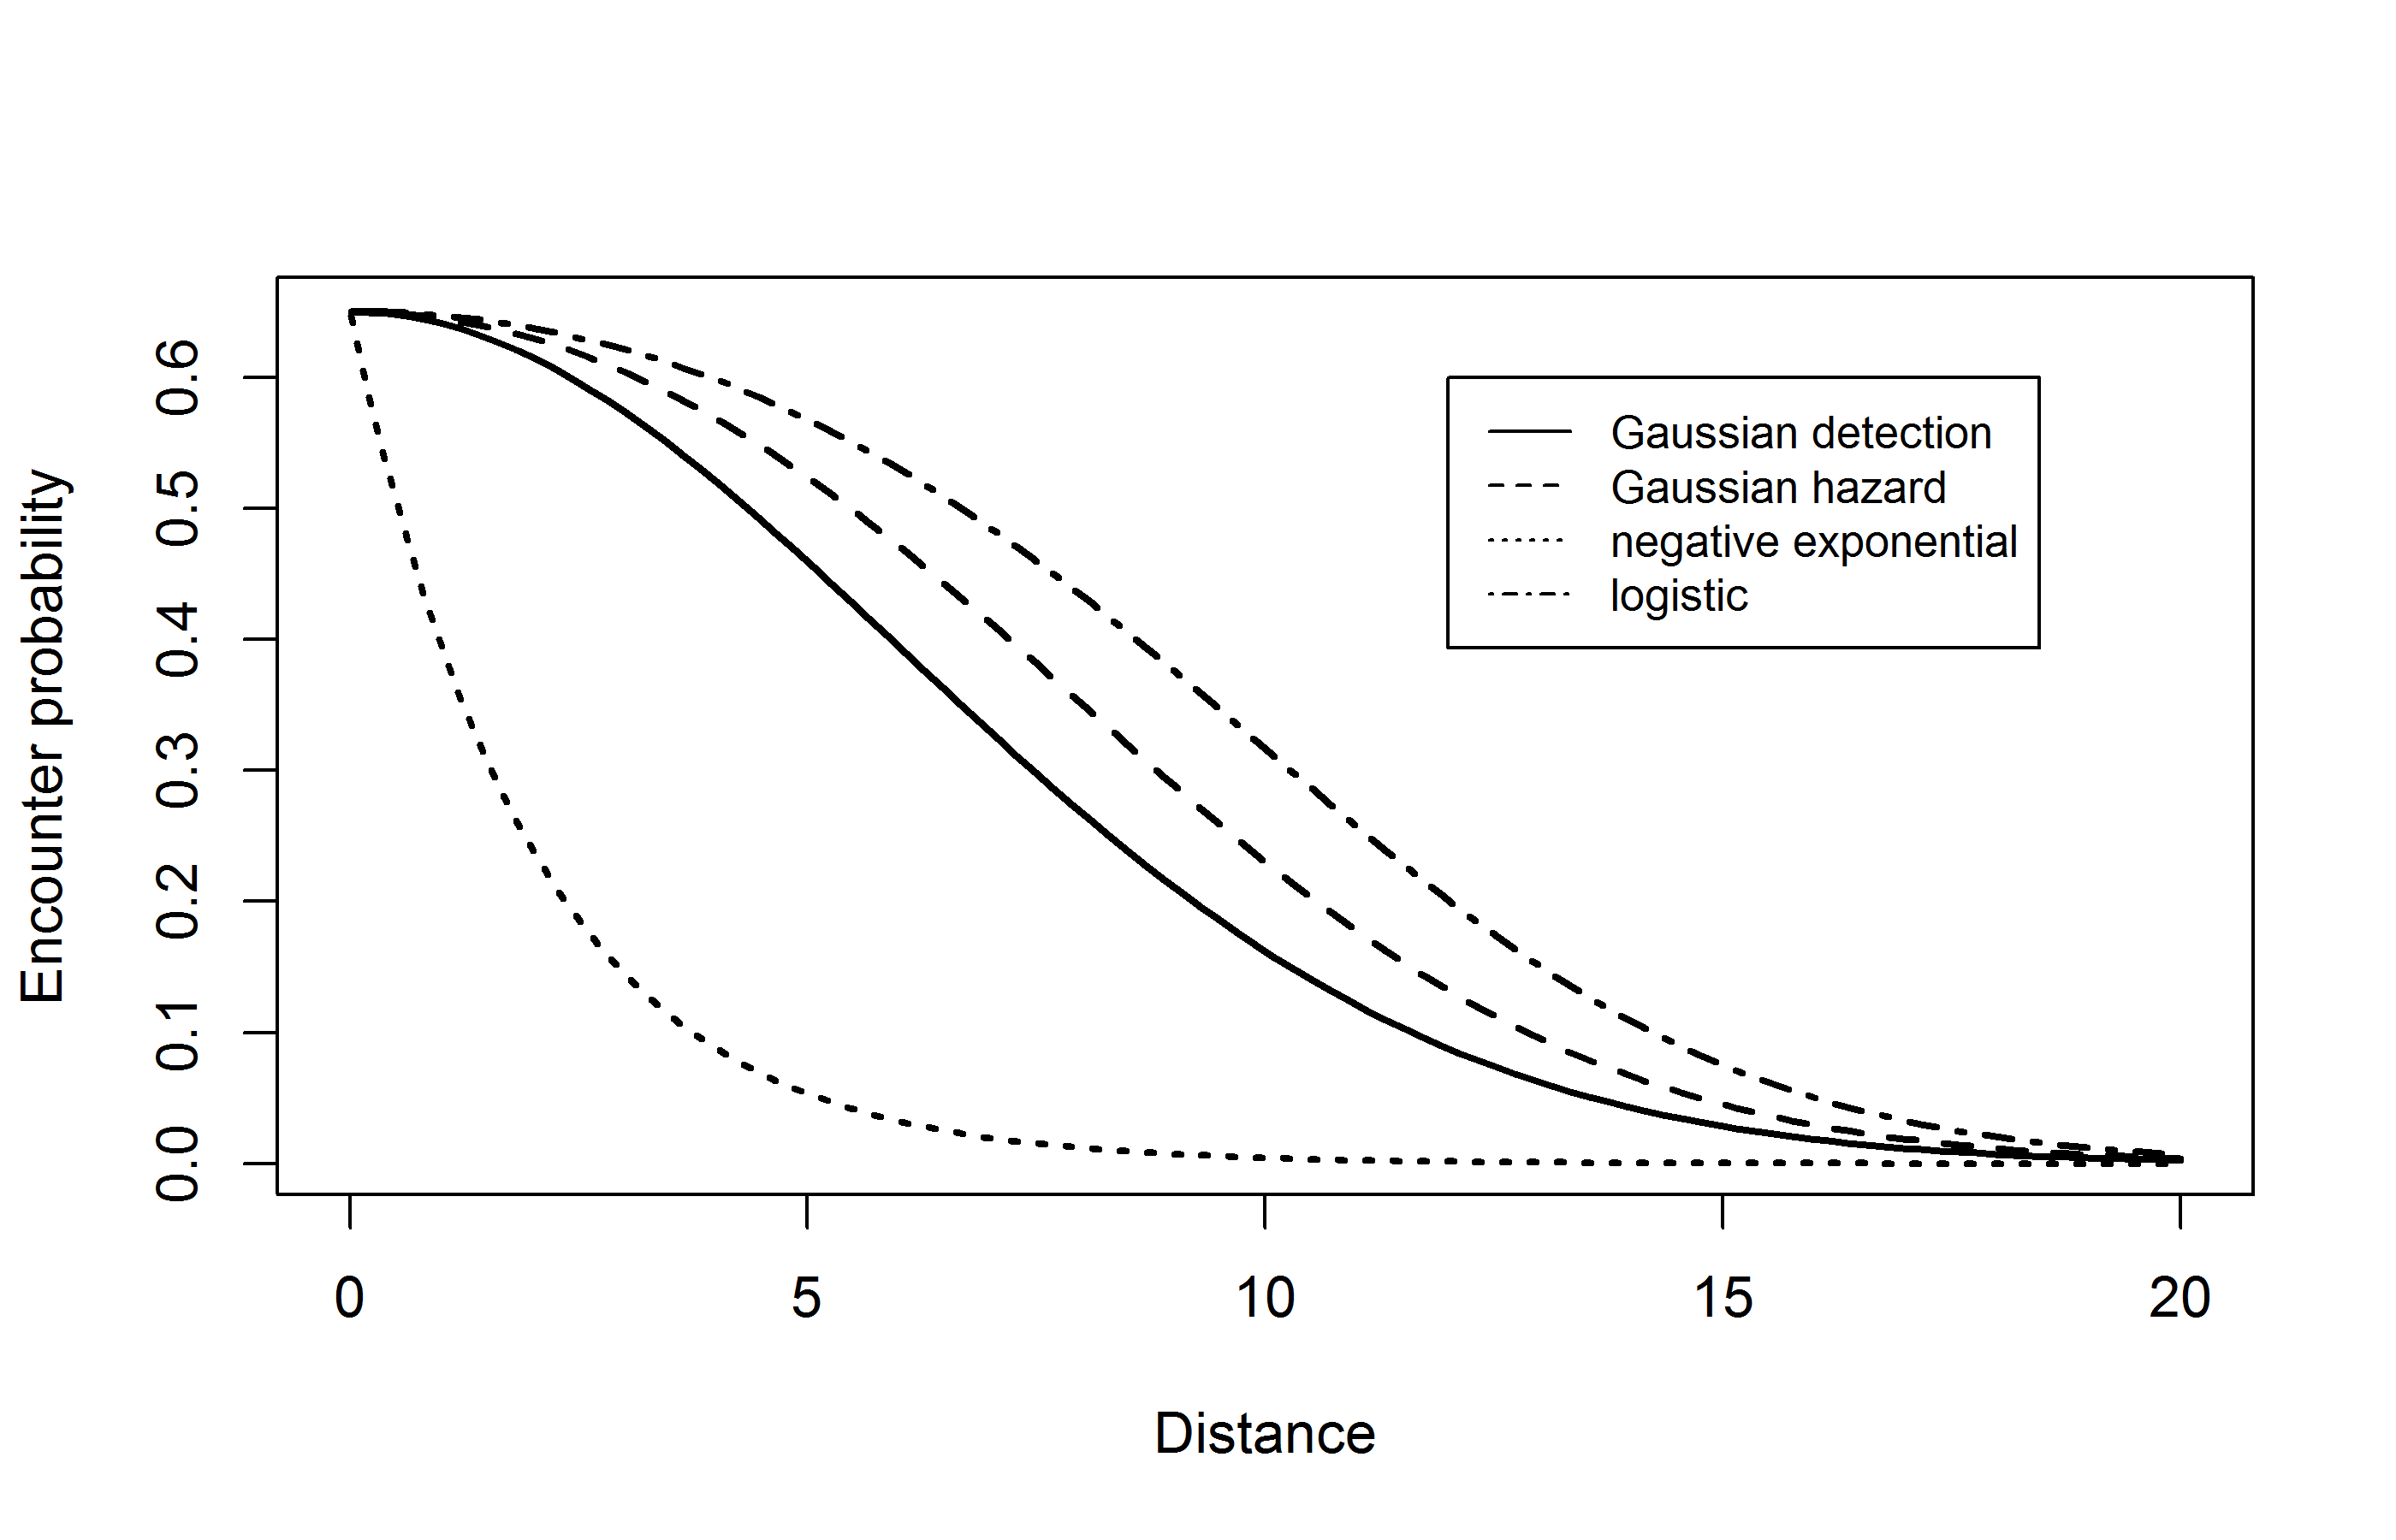
\includegraphics[height=2.75in]{Ch5-SCR0/figs/det_functions}
\end{center}
\caption{Some common encounter probability models showing the
  characteristic monotone decrease of encounter probability with
  distance between activity center and trap location.
{\bf  XXXX Suggest capitalizing axis labels. Why do they have
   different intercepts? XXXX }
}
\label{scr0.fig.detfuncs}
\end{figure}
% XXXX I think we should have a table that lists the standard
% encounter models and their definitions. This needs to stand out and
% be very clear so that people can easily reference this stuff XXXX
% Note that the bivariate normal model
%is equivalently represented as
%\begin{equation}
%\log(p_{ij})  = \log(p_{0}) - \alpha_{1} *||{\bf s}_{i}-{\bf x}_{j}||^2
%\label{scr0.eq.norm}
%\end{equation}
%which we make use of sometimes in specifying the model in the \bugs language.
%We would always like to be clear that encounter probability depends on individual activity
%centers {\it and} trap locations {\it and} parameter(s) $\theta$, and
%so it would be ideal to write $p({\bf s}_{i},{\bf x}_{j}; \theta)$ or
%something similar. However, this can be extremely unwieldy and
%clutter up what are otherwise extremely simple mathematical
%expressions and formulae. As such, we will usually abbreviate these
%various dependencies by writing $p_{ij}$ or sometimes $p_{\theta,ij}$,
%understanding that $p_{ij}$ is actually a function of the various important
%quantities.
Whatever model we choose for encounter probability, we should always
keep in mind that the activity center for individual $i$, ${\bf
  s}_{i}$, is an unobserved random variable.  To be precise about this
in the model, we should express the observation model as
\[
y_{ij}|{\bf s}_{i} \sim \mbox{Binomial}(K, p({\bf s}_{i};\alpha_{1}))
\]
but sometimes, for notational simplicity, we abbreviate this by
omitting some of the arguments to $p$.




\subsection{Definition of home range center}

We define an individual's home range as {\it the area used by an
  organism during some time period} which has a clear meaning for most
species regardless of their biology.
%Some will be offended by our use of the concept of ``home range
%center'' and question whether such notions as home ranges are useful
%for some (or perhaps {\it any}) particular species.  Indeed, the idea
%of a home range is a vague and purely phenomenological construct
%anyway.  Despite this, it doesn't really matter whether or not a home
%range makes sense for a particular species - individuals of any
%species inhabit {\it some} region of space and
We therefore define the
home range center (or activity center) to be the center of the space that individual
was occupying (or using) during the period in which traps were
active. Thinking about it in that way, it could even be observable
(almost) as the centroid of a very large number of radio fixes over
the course of a survey period or a season.  Thus, this practical
version of a home range center in terms of space usage is a
well-defined construct regardless of whether one thinks the home range
itself is a meaningful concept.
  We use the terms home range center and
activity center interchangeably, and we recognize that this is a
transient thing which applies only to a well-defined period of study.


\subsection{Distance as a latent variable}

If we knew precisely every ${\bf s}_{i}$ in the population (and
population size $N$), then the model specified by
Eqs. \ref{scr0.eq.bin} and \ref{scr0.eq.logit} would be just an
ordinary logistic regression-type of a model (with covariate $d_{ij}$)
which we learned how to fit using {\bf WinBUGS} previously
(Chapt. \ref{chapt.glms}).  However, the activity centers are
unobservable even in the best possible circumstances. In that case,
$d_{ij}$ is an unobserved variable, analogous to the situation in
classical random effects models.  We need to therefore extend the
model to accommodate these random variables with an additional model
component -- the random effects distribution.  The customary
assumption is the so-called ``uniformity assumption,'' which is to
assume that the ${\bf s}_{i}$ are uniformly distributed over space
(the obvious next question: ``which space?'' is addressed below).  This
uniformity assumption amounts to a uniform prior distribution on ${\bf
  s}_{i}$, i.e., the pdf of ${\bf s}_{i}$ is constant, which we may
express
\begin{equation}
	\Pr({\bf s}_{i}) \propto \mbox{constant}
\label{scr0.eq.sprior}
\end{equation}
 As it turns out, this assumption is usually not precise
enough to fit SCR models in practice for reasons we discuss
shortly.  We will give another way to represent this prior
distribution that is more concrete, but depends on specifying the
``state-space'' of the random variable ${\bf s}_{i}$. The term
state-space is a technical way of saying ``the space of all possible
outcomes'' of the random variable.

\begin{comment}
To summarize the preceding model developing, a basic SCR model is
defined by 3 essential components:
\begin{itemize}
\item[(1)] Observation model: $y_{ij}|{\bf s}_{i} \sim \mbox{Bin}(K, p_{ij})$
\item[(2)] Encounter probability model, such as:
$p_{ij} = p_{0}*\exp(-\alpha_{1} *||{\bf s}_{i}-{\bf x}_{j}||^2)$
\item[(3)] Point process model: $\Pr({\bf s}_{i} ) \propto \mbox{\tt const}$
\end{itemize}
Therefore, the SCR model is little more than an ordinary
capture-recapture model for closed populations. It is such a model,
but augmented with a set of ``individual effects'', ${\bf s}_{i}$,
which relate some sense of individual location to encounter
probability.
\end{comment}



































\section{ The Binomial Point Process Model}
\label{scr0.sec.bpp}

In the SCR model, the individual activity centers are unobserved and thus we
treat them as random effects. Specifically,
the collection of individual activity centers ${\bf s}_{1},\ldots,
{\bf s}_{N}$ represents a realization of a {\it binomial point process}
\citep[][p. 61]{illian_etal:2008}.  The binomial point process (BPP)
is analogous to a Poisson point process in the sense that it
represents a ``random scatter'' of points in space -- except that the
total number of points is {\it fixed}, whereas, in a Poisson point
process, it is random (having a Poisson distribution).  As an example,
we show in Fig. \ref{scr0.fig.bpp} locations of 20 individual activity
centers (black dots) in relation to a grid of 25 traps. For a Poisson
point process the number of such points in the prescribed state-space
would be random whereas often we will simulate fixed numbers of
points, e.g., for evaluating the performance of procedures such as how
well does our estimator perform with $N=50$?
\begin{figure}[ht]
\begin{center}
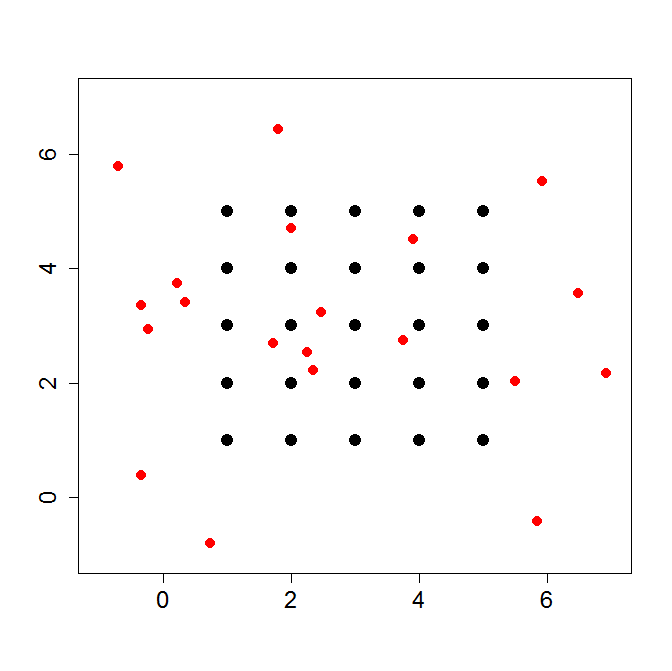
\includegraphics[height=2.5in]{Ch5-SCR0/figs/binomialpoint}
\end{center}
\caption{Realization (small dots) of a binomial point process with $N=20$. The
  large dots represent trap locations.
}
\label{scr0.fig.bpp}
\end{figure}

It is natural to consider a binomial point process in the context of
capture-recapture models because it preserves $N$ in the model and thus
preserves the linkage directly with closed population models. In fact,
under the binomial point process model, model $M_0$ and other closed
models are simple limiting cases of SCR models, i.e., they arise as the
coefficient on distance ($\alpha_1$ above) tends to 0.

While we often will express SCR models ``conditional-on-$N$'', it will
sometimes be convenient to impose specific prior distributions on
$N$. By assuming $N$ has a binomial distribution, we can make use of
data augmentation, our preferred tool, for Bayesian analysis of the
models as in Chapt. \ref{chapt.closed}, thus yielding a
methodologically coherent approach to analyzing the different classes
of models. We might also assume that $N$ has a Poisson distribution in
some cases (see Chapt. \ref{chapt.hscr}). Of course, the two
assumptions are closely related in the usual limiting sense.
% XXXX Suggest citing Efford and Fewster (2012) here, as well as Sandland and
% Cormack (1984). And elaborate on distinction between modeling E[N]
% and N XXXX

One consequence of having fixed $N$ in the BPP model is that the model
is not strictly a model of ``complete spatial randomness''. This is
because if one forms counts $n(A_{1}),\ldots, n(A_{k})$ in any set of
disjoint regions of the state-space, say $A_{1}, \ldots, A_{k}$, then
these counts are {\it not} independent.  In fact, they have a
multinomial distribution \citep[see][p. 61]{illian_etal:2008}. Thus,
the BPP model introduces a slight bit of dependence in the
distribution of points. However, in most situations this will have no
practical effect on any inference or analysis and, as a practical
matter, we will usually regard the BPP model as one of spatial
independence among individual activity centers because each activity
center is distributed independently of each other activity
center. Despite this implicit independence we see in
Fig. \ref{scr0.fig.bpp} that {\it realizations} of randomly
distributed points will typically exhibit distinct
non-uniformity. Thus, independent, uniformly distributed points will
almost never appear regularly, uniformly or systematically
distributed. For this reason, the basic binomial (or Poisson) point
process models are enormously useful in practical settings since they
allow for a range of distribution patterns without violating the
assumption of spatial randomness.  More relevant for SCR models is
that we actually have a little bit of data for some individuals and
thus the resulting posterior point pattern can deviate strongly from
uniformity, a point we come back to repeatedly in this book.  The
uniformity hypothesis is only a {\it prior} distribution which is
directly affected by the quantity and quality of the observed data, to
produce a posterior distribution which may appear distinctly
non-uniform.  In addition, we can build more flexible models for the
point process, which we take up in Chapt. \ref{chapt.state-space}.


\subsection{The state-space of the point process}

Shortly we will focus on Bayesian analysis of the model SCR0 with $N$
known so that we can gain some basic experience with important
elements of the model.  To do this, we note that the individual
activity centers ${\bf s}_{i},\ldots, {\bf s}_{N}$ are unknown
quantities and we will need to be able to simulate each ${\bf s}_{i}$
in the population from the posterior distribution.  In order to
simulate the ${\bf s}_{i}$, it is necessary to describe precisely the
region over which they are distributed. This is the quantity referred
to above as the state-space, which is sometimes called the {\it
  observation window} in the point process literature. We denote the
state-space henceforth (throughout this book) by ${\cal S}$ , which is
a region or a set of points comprising the potential values (the
support) of the random variable ${\bf s}$. Thus, an equivalent
explicit statement of the ``uniformity assumption'' is
\[
{\bf s}_{i} \sim \mbox{Uniform}({\cal S})
\]
where ${\cal S}$ is a precisely defined region. e.g., in Fig.
\ref{scr0.fig.bpp}, ${\cal S}$ is the square defined by $[-1,7] \times
[-1, 7]$. Thus each of the $N=20$ points were generated by randomly
selecting each coordinate on the line $[-1, 7]$. When points are
distributed uniformly
over some region, the point process is usually called a {\it
  homogeneous point process}.



\subsubsection{Prescribing the state-space}
\label{scr0.sec.ss}
% XXXX Somewhere we should mention that the state-space is often
% called the "observation window" in spatial point process
% literature. It could also be called the "support" for s. And in
% secr, it is called a "mask". XXXX

Evidently, we need to define the state-space, ${\cal S}$. How can we
possibly do this objectively? Prescribing any particular ${\cal S}$
seems like the equivalent of specifying a ``buffer'' which we
have criticized as being ad hoc. How is it, then, that the
choice of a state-space is {\it not} ad hoc?
As we observed in Chapt. \ref{chapt.closed}, it is true
that $N$ increases with ${\cal S}$, but only at the same rate as the
area of ${\cal S}$ increases under the prior assumption of constant
density. As a result, we say that density is invariant to ${\cal S}$
{\it as long as ${\cal S}$ is sufficiently large}. Thus, while choice of
${\cal S}$ is (or can be) essentially arbitrary, once ${\cal S}$ is
chosen, it defines the population being exposed to sampling, which
scales appropriately with the size of the state-space.

For our simulated system developed previously in this chapter, we
defined the state-space to be a square within which our trap array was
centered. For many practical situations this might be an acceptable
approach to defining the state-space, i.e., just a rectangle around
the trap array.
%We provide an example
%of this in sec. \ref{scr0.sec.wolverine} below in which the trap array is
%irregular and also situated within a realistic landscape that is
%distinctly irregular.
%In general, it is most practical to define the
%state-space as a regular polygon (e.g., rectangle) containing the trap
%array without differentiating unsuitable habitat.
Although defining the state-space to be a regular polygon has
computational advantages (e.g., we can implement this more efficiently
in {\bf BUGS} and cannot for irregular polygons), a regular polygon
induces an apparent problem of admitting into the state-space regions
that are distinctly non-habitat (e.g., oceans, large lakes, ice
fields, etc.).  It is difficult to describe complex regions in
mathematical terms that can be used in {\bf BUGS}. As an alternative,
we can provide a representation of the state-space as a discrete set
of points which the {\bf R} package \mbox{\tt secr}
\citep{efford:2011} permits (\mbox{\tt secr} uses the term ``mask''
for what we call the state-space).  Defining the state-space by a
discrete set of points is handy because it allows specific points to
be deleted or not, depending on whether they represent available or
suitable habitat (see Sec.  \ref{scr0.sec.discrete}).  We can also
define the state-space as an arbitrary collection of polygons stored
as a GIS shapefile which can be analyzed easily by MCMC in {\bf R}
(see Sec. \ref{mcmc.sec.state-space}), but not so easily in the {\bf
  BUGS} engines.  In what follows below we provide an analysis of the
wolverine camera trapping data, in which we define the state-space to
be a regular continuous polygon (a rectangle).


\subsubsection{Invariance to the state-space}
\label{scr0.sec.invariance}

% XXXX Suggest shortening this paragraph to just say that p=0 at d=B
% when B is large enough. I don't think there is a need to bring up
% the multinomial likelihood XXXX
We will assert for all models we consider in this book that density is
invariant to the size and extent of ${\cal S}$, if ${\cal S}$ is
sufficiently large, and as long as our model relating $p_{ij}$ to
${\bf s}_{i}$ is a decreasing function of distance.  We can prove this
easily by drawing an analogy with a 1-d case involving distance
sampling.  Let $y_{j}$ be the number of individuals captured in some
interval $[d_{j-1},d_{j})$, and define $d_{J} = B$ for some large
value of $B$.
 The observations from a survey are $y_{1},\ldots,y_J$
and the likelihood is a multinomial likelihood, so the log-likelihood
is of the form
\[
\mbox{logL}(y_{1},\ldots,y_{J}) = \sum_{j=1}^{J} y_{j} \log( \pi_{j} )
\]
where $\pi_{j}$ is the probability of detecting an individual in
distance class $j$, which depends on parameters of the detection
function (the manner of which is not relevant for the present
discussion).  Choosing $B$ sufficiently large guarantees that
$\mathbb{E}(y_{J}) = 0$ and therefore the observed frequency in the
``last cell'' contributes nothing to the likelihood, in regular
situations in which the detection function decays monotonically with
distance and prior density is constant.  We can think of $B$ as being
related to the state-space in an SCR model; $B \times L$, $L$ being
the length of the transect, defines a rectangular state-space, ${\cal
  S}$. Thus, if we choose $B$ large enough, then we ensure that the
expected trap-frequencies beyond $B$ will be 0, and thus contribute
nothing to the likelihood.

Sometimes our estimate of density can be affected by choosing ${\cal
  S}$ too small. However, this might be sensible if ${\cal S}$ is
naturally well-defined. As we discussed in Chapt.~\ref{chapt.intro},
{\it choice of ${\cal S}$ is part of the model}, and thus it is
sensible that estimates of density might be sensitive to its
definition in problems where it is natural to restrict ${\cal S}$.
One could imagine, however, that in specific cases where you're
studying a small population with well-defined habitat preferences,
that a problem could arise because changing the state-space around
based on differing opinions and GIS layers might have substantial
changes on the density estimates and hence those of population
size. But this is a real biological problem and a natural consequence
of the spatial formalization of capture-recapture models -- a feature,
not a bug or some statistical artifact -- and it should be resolved
with better information, research, and thinking.  For situations where
there is not a natural choice of ${\cal S}$, we should default to
choosing ${\cal S}$ to be very large in order to achieve invariance
or, otherwise, evaluate sensitivity of density estimates by trying a
couple of different choices of ${\cal S}$. This is a standard
``sensitivity to prior'' argument that Bayesians always have to be
conscious of.  We demonstrate this in our analysis of section
\ref{scr0.sec.wolverine} below. As an additional practical
consideration, we note that the area of the state-space ${\cal S}$
affects data
augmentation. If you increase the size of ${\cal S}$, then there are more
individuals to account for and therefore the size of the augmented
data set $M$ must increase. This has computational implications.

\subsection{Connection to model $M_h$ and distance sampling}
 \label{scr0.sec.scrmh}

SCR models are closely related to  ``model
$M_h$'' and also distance sampling.  In SCR models,
heterogeneity in encounter probability is induced by both the effect
of distance in the model for detection probability and also from
specification of the state-space. Hence, the state-space  is an
explicit element of the model.
To understand this, suppose activity centers have the uniform distribution:
\[
{\bf s} \sim \mbox{Uniform}({\cal S})
\]
and encounter probability is a function of ${\bf s}$, denoted by
 $p({\bf s}) = p(y=1|{\bf s})$.
For example, under Eq. \ref{scr0.eq.logit}
we have that
\[
p({\bf s}) = \mbox{logit}^{-1} ( \alpha_{0} + \alpha_1 ||{\bf
  x}_{j}-{\bf s}_{i} || )
\]
and we can work out, either analytically or empirically, what is the
implied distribution of $p$ for a population of individuals.
Fig. \ref{scr0.fig.buffereffect} shows a
histogram of $p$ for a hypothetical population of 100000 individuals
on a state-space enclosing our $5 \times 5$ trap array above, under
the logistic model for distance given by Eq. \ref{scr0.eq.logit}
with
 buffers of 0.2, 0.5
and 1.0. We see the mass shifts to the left as the buffer increases,
implying more individuals with lower encounter probabilities, as their
home range centers increase in distance from the trap array.

% XXXX Would be nice if x-axes were the same XXXX
\begin{figure}[ht]
\begin{center}
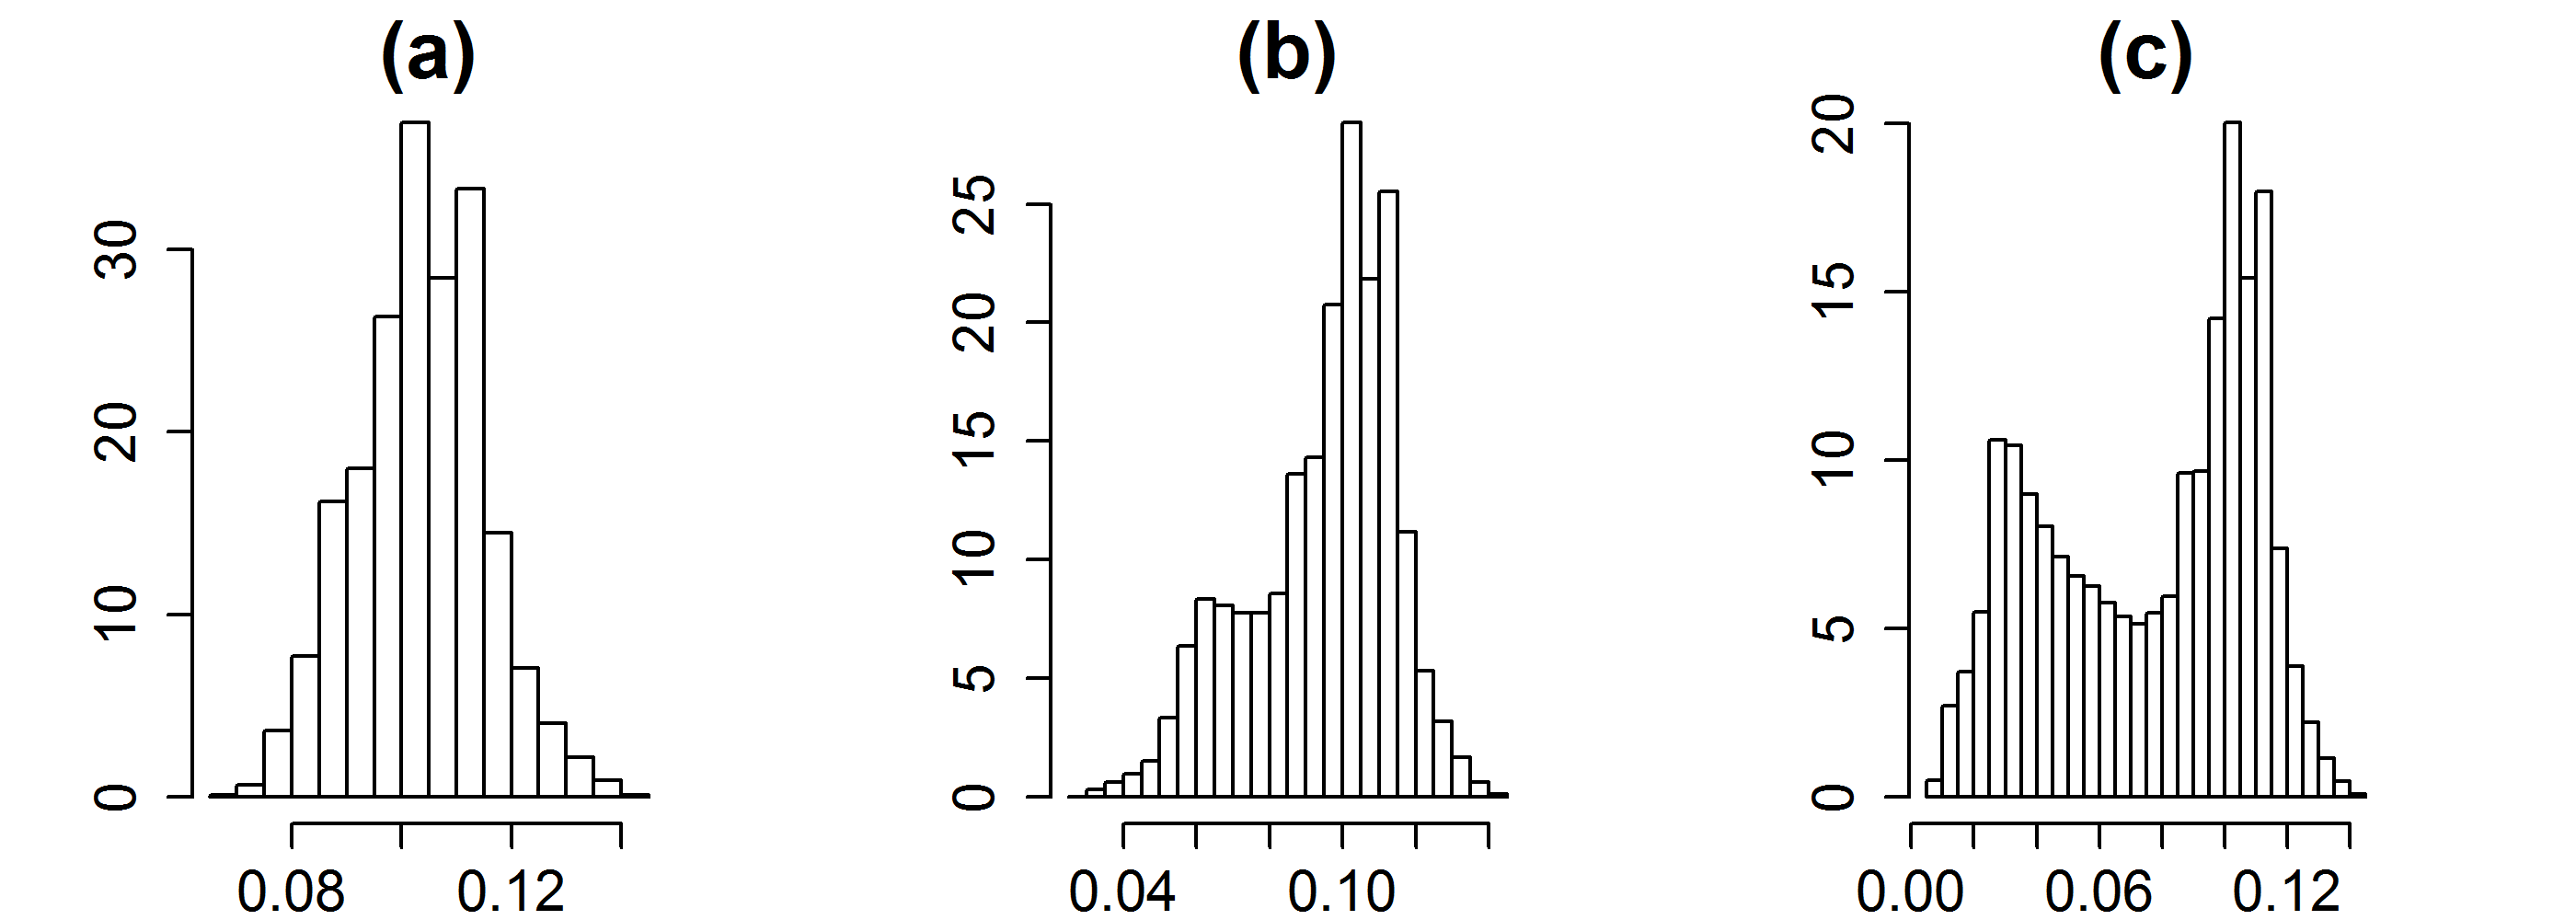
\includegraphics[width=4.5in,height=1.6in]{Ch5-SCR0/figs/Mh_buffer}
\end{center}
\caption{Implied distribution of $p_{i}$ for a population
  of individuals as a function of the size of the state-space buffer
around the trap array. The state-space buffer is 0.2, 0.5 and 1.0 for
panels (a), (b), (c), respectively.
In each case, the trap array is fixed and centered within a
  square state-space.
}
\label{scr0.fig.buffereffect}
\end{figure}

Another way to understand this is by representing ${\cal S}$ as a set
of discrete points on a grid. In the coarsest possible case where
${\cal S}$ is a single arbitrary point, then every individual has
exactly the same $p$. As we increase the number of points in ${\cal
  S}$,  more distinct values of $p$ are possible. Indeed, when
${\cal S}$ is characterized by discrete points then SCR models are
precisely a type of finite-mixture model \citep{norris_pollock:1996,
  pledger:2000}, except, in the case of SCR models, we have some information about which
group an individual belongs to (i.e., where their activity center is), as
a result of which traps they're captured in.
\begin{comment}
This context suggests the problem raised by \citet{link:2003}. He
showed that in most practical situations $N$ may not be identifiable
across classes of mixture distributions which in the context of SCR
models is the pair $(g, {\cal S})$.  With SCR models, however,
we do obtain some direct information about ${\bf s}$ for the
encountered individuals and,
therefore, it may be reasonable to expect that
$N$ is identifiable across models characterized by $(g,{\cal
  S})$.
\end{comment}


It is also worth re-emphasizing that the basic SCR encounter model is a binomial
encounter model in which distance is a covariate. As such, it is
strikingly similar to classical distance sampling models
\citep{buckland_etal:2001}. Both have distance as a covariate but in
classical distance sampling problems the focus is on the distance
between the observer and the animal at an instant in time, not the
distance between a trap and an animal's home range center. As a
practical matter, in distance sampling, ``distance'' is {\it observed}
for those individuals that appear in the sample. Conversely, in SCR
problems, it is only imperfectly observed (we have partial information
in the form of trap observations).  Clearly, it is preferable to
observe distance if possible, but distance sampling requires field
methods that are not practical in many situations, e.g. when
studying carnivores such as bears or large cats. Furthermore, SCR
models allow us to relax many of the assumptions made in classical
distance sampling, such as perfect detection at distance zero, and SCR
models allow for estimates of quantities other than density, such as
home range size, and space usage (see Chapts. \ref{chapt.rsf} and
\ref{chapt.ecoldist}).
















\section{The Implied Model of Space Usage}
\label{scr0.sec.implied}


% bivariate normal a null model for "central place forager" but even
% for a non-central place foragter, the activity center is a transient
% thing so it produces an approximation over a short period.
% whilt it is a simple model we only have sparse movement observations
% in virtually all practical c-r situations
We developed the basic SCR model in terms of a latent variable, ${\bf
  s}$, the home range center or activity center.  Surely then, the
encounter probability model, which relates encounter of individuals in
specific traps to ${\bf s}$ must somehow imply a certain model for
home range geometry and size -- ``space usage''.  Here we explore the
nature of that relationship and we argue that any given detection
model implies a model of space usage -- i.e., the amount and extent of
area used some prescribed percentage of the time. So we might say,
for example, 95\% of animal movements are within some distance from an
individual's activity center.  While we have used the term ``home
range'' or similar, what we really mean to imply is something that
would be more clearly identified as
resource selection or space usage (the latter term meaning resource
selection, when the resource is only homogeneous space).
%If the resource is only
%homogeneous space, i.e., all space is equally suitable to the animal,
%then we mean space usage is a more descriptive term but,
%otherwise (Chapt. \ref{chapt.rsf}) we take on the more genereal
%problem of modeling resource selection.

Intuitively, the detection function of SCR models is related to home
range area or space usage of individuals.  Indeed, it is natural
to interpret the detection model as the composite of two processes:
movement of an individual about its home range i.e., how it uses space
within its home range (``space usage''), and detection {\it
  conditional on use} in the vicinity of a trapping device.
It is natural to decompose encounter probability according to:
\[
 \Pr(\mbox{encounter at } {\bf x}|{\bf s})
 = \Pr(\mbox{encounter}| \mbox{usage of } {\bf x}, {\bf s})
\Pr(\mbox{usage of } {\bf x}|{\bf s}).
\]
In practice it might make sense to think about the first component, \newline
i.e., $\Pr(\mbox{encounter} | \mbox{usage of } {\bf x}, {\bf s})$ as
being a constant (e.g., if traps are located within arbitrarily small
grid cells) and then, in that case, the encounter probability model is
directly proportional to this model for individual movements about
their home range center determining the use frequency of each ${\bf x}$.
This is a sensible heuristic model for what ecologists would call a
central place forager although, as we have stated previously, it may
be meaningful as a description of transient space usage as well (that
is, the space usage during the period of sampling).

To motivate a specific model for space usage, imagine
the area we are interested in consists of some large
number of small pixels (i.e. we're looking at a discrete
representation of space), and that we have some kind of
perfect observation device (e.g., continuous telemetry) so that we
observe every time an individual moves into a pixel. After a long
period of time we observe an enormous sample size of ${\bf x}$
values. We tally those up into each pixel, producing the frequency
$m({\bf x},{\bf s})$, which is something like the ``true'' usage of
pixel ${\bf x}$ by individual with activity center
${\bf s}$.  So, then, the usage model
should be regarded as a probability mass function for these counts
and, naturally, we regard the counts $m({\bf x},{\bf s})$ as a
multinomial observation with probabilities $\pi({\bf x}|{\bf s})$ and
prescribe a suitable model for $\pi({\bf x}|{\bf s})$ that describes
how use events should accumulate in space. A natural null model for
$\pi({\bf x}|{\bf s})$ has a decreasing probability of use as ${\bf
  x}$ gets far away from ${\bf s}$; i.e., animals spend more time
close to their activity centers than far away.  We can regard points
used by the individual with activity center ${\bf s}$ as the
realization of a point process with conditional intensity:
\begin{equation}
\pi({\bf x}|{\bf s}) =  \frac{ k({\bf x},{\bf s}) }{ \sum_{x} k({\bf
    x},{\bf s}) }
\label{scr0.eq.ud}
\end{equation}
where $k({\bf x},{\bf s})$ is any positive function.
In continuous space, the equivalent representation would be:
\[
\pi({\bf x}|{\bf s}) =  \frac{ k({\bf x},{\bf s}) }{ \int k({\bf
    x},{\bf s}) dx }.
\]
%If we represent our landscape by discrete pixels, then this is the
%equivalent form is:
%In continuous
%space, we would just replace the denominator with an integral, but the
%discrete space formulation of this is relevant to most practical
%problems.
%This is the
%conditional intensity function of a point processes
% looks like a
% type of resource selection function (RSF)
%\citep[e.g.,][Ch. 8]{manly_etal:2001}.
Clearly the space used by an individual will be proportional
to whatever kernel, $k({\bf x},{\bf s})$, we plug-in for the numerator.
If we use a negative exponential function, then this produces a
standard
resource selection function (RSF) model
\citep[e.g.,][Ch. 8]{manly_etal:2002}.
But, here we use a Gaussian kernel, i.e.,
\[
 k({\bf x},{\bf s})= \exp(  -d({\bf x},{\bf s})^{2}/(2\sigma^{2}))
\]
so that contours of the probability of space usage resemble a
bivariate normal or Gaussian probability distribution function.

To apply this model of space-usage to SCR problems we  allow for imperfect
detection by introducing a constant ``thinning rate'' of the true
counts $m({\bf x},{\bf s})$. Then, this
yields, precisely, our Gaussian encounter probability model where the
thinning rate is our baseline encounter probability $p_0$.
The main take-away point here is that underlying most SCR models is
some kind of model of space-usage, implied by the
specific choice of $k({\bf x},{\bf s})$.
Whether or not we have perfect sampling devices, the function we use
in the encounter probability model equates to some conditional
distribution of points, a utilization distribution,
 as in
Eq. \ref{scr0.eq.ud}, from which we can compute effective home range
area, i.e., the area that contains some percent of the mass of a
probability distribution proportional to
 $k({\bf x},{\bf
  s})$; e.g.,  95\% of all space used by an individual with activity
center ${\bf s}$.


\begin{comment}
Whether or not a
point $x$ is {\it used} (at all) depends on some unknown rate of use
by the individual over whatever period of time the devices are
active. This is something we can't hope to estimate or model in most
cases but we imagine that over a period of time usage is characterized
by a rate of usage $\lambda_{0}$ so that amount of usage -- the number
of times individual $s$ enters $x$, is:
\[
m({\bf x},{\bf s}) = Poisson(\lambda_{0} \pi(x|s) )
\]
which isn't really an important assumption because note that by
conditioning on the total again it retains the (natural) multinomial
distribution.
Moreover, if our detection devices are {\it imperfect} then all this
does is introduce another constant into the above expression that we
might as well confound with $\lambda_{0}$. Thus a background use or
movement rate, and a time interval over which use accumulates, is
completely confounded with efficacy of our sampling devices that
measures space usage.

If our sampling devices do not record total visits during a period but
rather just ``whether or not'' an individual visits,
then observe a binary observation $y$ which we can think of as being
related to the {\it latent} counts $m(x,s)$ by $Pr(y=1) = Pr(m(x,s)>0)$
which occurs with probability:
\begin{equation}
\Pr(y=1) = 1-exp(-\lambda_{0} \pi(x|s))
\label{scr0.eq.hazard}
\end{equation}
which is called the ``hazard-rate model'' in classical distance sampling
applications \citep{buckland_etal:2002}.
This is why we like the cloglog link function in \citep{royle_etal:2009ecol}.
So this all comes about by introducing a latent process of ``usage''
accumulating over time.
We could just as well say $Pr(y=1) \propto \pi(x|s)$ which is the
half-normal model (See Chapt. \ref{chapt.poisson-mn}).
\end{comment}


\subsection{Bivariate normal case}

One encounter model that allows direct analytic computation
of home range area is the Gaussian encounter probability model
\[
p({\bf x},{\bf s}) = p_{0} \exp(-\frac{1}{2\sigma^2} ||{\bf x}-{\bf s}||^2).
\]
For this model, encounter probability is proportional to the kernel of
a bivariate normal (Gaussian) pdf and so the natural interpretation is
that in which movement outcomes (or successive locations of an
individual) are draws from a bivariate normal distribution with
standard deviation $\sigma$. We say that use of this model implies a
 bivariate normal model of space usage.
Under this model we can compute precisely the effective home range
area. In particular, if use outcomes are bivariate normal, then
$||{\bf x}-{\bf s}||^2$ has a chi-square distribution with 2 d.f. and
the quantity $B(\alpha)$ that encloses $(1-\alpha)$\% of all realized
distances i.e., $\Pr(d\le B(\alpha)) = 1-\alpha$, is $B(\alpha) =
\sigma*\sqrt{q(\alpha,2)}$ where $q(\alpha,2)$ is the $0.05$
chi-square critical value on $2$ df. For example, to compute $q(.05,
2)$ in {\bf R} we execute the command \mbox{\tt qchisq(.95,2)} which
is $q(2,\alpha) = 5.99$. Then, for $\sigma=1$, $B(\alpha) =
1*\sqrt{5.99} = 2.447$.  Therefore 95\% of the points used will be
within 2.447 (standard deviation) units of the home range center. So,
in practice, we can estimate $\sigma$ by fitting the bivariate normal
encounter probability model to some SCR data, and then use the
estimated $\sigma$ to compute the ``95\% radius'', say $r_{.95} =
\sigma \sqrt{5.99}$, and convert this to the {\it 95\% use area} --
the area around ${\bf s}$ which contains 95\% of the movement outcomes
-- according to $A_{.95} = \pi r_{.95}^{2}$.

An alternative bivariate normal model is the bivariate normal hazard
rate model:
\begin{equation}
p({\bf x},{\bf s}) = 1-\exp(-\lambda_{0}*\exp(-\frac{1}{2\sigma^{2}} ||{\bf x}-{\bf s}||^2))
\label{scr0.eq.hazard}
\end{equation}
We use $\lambda_{0}$ here because this parameter, the baseline
encounter {\it rate}, can be $>1$.  This arises by assuming the latent
``use frequency'' $m({\bf x},{\bf s})$ is a Poisson random variable
with intensity $\lambda_0 k({\bf x},{\bf s})$. The model is distinct
from our Gaussian encounter model $p({\bf x},{\bf s}) = p_0 k({\bf
  x},{\bf s})$ used previously, although we find that they produce
similar results in terms of estimates of density or 95\% use area, as
long as baseline encounter probability is low.  We discuss these two
formulations of the bivariate normal model further in
Chapt. \ref{chapt.poisson-mn}.

\subsection{Empirical analysis}

For any encounter model we can compute space usage quantiles
empirically by taking a fine grid of points and either simulating
movement outcomes with probabilities proportional to $p({\bf x},{\bf
  s})$ and accumulating area around ${\bf s}$, or else we can do this
precisely by varying $B(\alpha)$ to find that value within which 95\%
of all movements are concentrated, i.e., the set of all ${\bf x}$ such
that $||{\bf x}-{\bf s}|| \le B(q)$.  Under any detection model,
movement outcomes will occur in proportion to $p({\bf x},{\bf s})$, as
long as the probability of encounter is constant, {\it conditional on
  use}, and so we can define our space usage distribution according
to:
\[
 \pi({\bf x}|{\bf s}) =\frac{p({\bf x},{\bf s})}{\sum_{x} p({\bf
     x},{\bf s}) }
\]
Given the probabilities $\pi({\bf x},{\bf s})$ for all ${\bf x}$ we
can find the value of $B(q)$, for any $q$, such that
\[
\sum_{{\bf x}
  \ni ||x-s|| \le B(q) } \pi({\bf x},{\bf s}) \le 1-q
\]
(here, we use $\ni$ to mean ``such that'').
We have a function called \mbox{\tt hra} in the \mbox{\tt scrbook}
package that computes the home range area for any encounter model and
prescribed parameter values. The help file for \mbox{\tt hra} has an
example of simulating some data.  The following commands illustrate
this calculation for two different bivariate normal models of space
usage:
% XXXX Can you add comments to this code? In the text, you have not been
% using "D" for distance, so you might consider changing this XXXX
{\small
\begin{verbatim}
##
## Define encounter probability model as R function
##
> pGauss2 <- function(parms,Dmat){
    a0 <- parms[1]
    sigma <- parms[2]
    lp <-  parms[1] -(1/(2*parms[2]*parms[2]))*Dmat*Dmat
    p <- 1-exp(-exp(lp))
    p
 }

> pGauss1 <- function(parms,Dmat){
    a0 <- parms[1]
    sigma <- parms[2]
    p <- plogis(parms[1])*exp( -(1/(2*parms[2]*parms[2]))*Dmat*Dmat )
    p
 }

##
## execute hra with sigma = .3993
##
> hra(pGauss1,parms=c(-2,.3993),plot=FALSE,xlim=c(0,6),ylim=c(0,6),
      ng=500,tol=.0005)

[1] 0.9784019
radius to achieve 95% of area:  0.9784019
home range area:  3.007353
[1] 3.007353


##  analytic solution
##  true sigma to produce area of 3
> sqrt(3/pi)/sqrt(5.99)
[1] 0.3992751
\end{verbatim}
}
What this means is that $B(q) = 0.978$ is the radius that
encloses about 95\% of all movements under the standard bivariate
normal encounter model.  Therefore, the area is about $\pi*.978*.978 =
3.007$ spatial units.  You can change the intercept of the model and
find that it has no effect.
The
true (analytic)
 value of $\sigma$ that produces a home range area of 3.0 is
$0.3993$ which is the value we initially plugged in to the \mbox{\tt
  hra} function. We can improve on the numerical approximation to home range
area (get it closer to $3.0$) by increasing
the resolution of our spatial grid (increase the \mbox{\tt
  ng} argument) along with the \mbox{\tt tol} argument.
%%%%  XXX note: tol and ng are redundant to some extent XXXX
%%%%%

We can also reverse this process, and find, for any detection model,
the parameter values that produce a certain $(1-q)$\% home range
area, which we imagine would be useful for doing simulation studies.
The function \mbox{\tt hra} will compute the value of the scale parameter
that achieves a certain target $(1-q)\%$ home range area, by
simply providing a non-null value of the variable \mbox{\tt
  target.area}. Here we use \mbox{\tt target.area = 3.00735} (from
above) to obtain a close approximation to the value $\sigma$ we
started with (the parameter argument is meaningless here):
{\small
\begin{verbatim}
> hra(pGauss1,parms=c(-2,.3993),plot=FALSE,xlim,ylim,ng=500,
       target.area=3.00735,tol=.0005)

Value of parm[2] to achieve 95% home range area of  3.00735:  0.3993674
\end{verbatim}
}

\subsection{Relevance of understanding space usage}

One important reason that we need to be able to deduce ``home range
area'' from a detection model is so that we can compare different
models with respect to a common biological currency.
Many encounter probability models have some ``scale parameter'', which
we might call $\sigma$ no matter the model, but this
relates to 95\% area in a different manner under each model.
Therefore, we want to be able to convert different models to the
same currency.
Another reason to understand the relationship between models of
encounter probability and space usage is that it opens the door to
combining traditional resource selection data from telemetry with
spatial capture-recapture data.  In Chapt. \ref{chapt.rsf} we consider
this problem, for the case in which a sample of individuals produces
encounter history data suitable for SCR models and, in addition, we
have telemetry relocations on a sample of individuals. This is
achieved by regarding the two sources of data as resulting from the
same underlying process of space usage but telemetry data produce
``perfect'' observations, like always-on camera traps blanketing a
landscape.  We use this idea to model the effect of a measured
covariate at each pixel, say $C({\bf x})$, on home range size and geometry
and, hence, the probability of encounter in traps.



\subsection{Contamination due to behavioral response}

Interpretation of encounter probability models as models
of animal home range and space usage can be complicated by a number of
factors, including whether traps are baited or not. In the case of
baited traps, this might lead to a
behavioral response (Sec. \ref{covariates.sec.behavior}) which could
 affect animal space usage. For example, if traps attract
animals from a long distance, it could make typical home ranges appear
larger than normal.
 More likely, in our view, it wouldn't
change the typical size of a range but would change how individuals
use their range e.g., by moving from baited trap to baited trap, so
that observed movement distances of individuals are typically larger
than normal. 

In other cases, the reliance on Euclidean distance in models for
encounter probability might be unrealistic, and can lead to biased
estimates of density \citep{royle_etal:2012ecol}.  For example,
animals might concentrate their movements along trails, roads, or
other landscape features. In this case, models that accommodate other
distance metrics can be considered. We present models based on
least-cost path in Chapt. \ref{chapt.ecoldist}. 


















\section{Simulating SCR Data}
\label{scr0.sec.simulating}

It is always useful to simulate data because it allows you to
understand the system that you're modeling and also calibrate your
understanding with specific values of the model parameters.
That is, you can
simulate data using different parameter values until you obtain data
that ``look right'' based on your knowledge of the specific situation
that you're interested in. Here we provide a simple script to
illustrate how to simulate spatial encounter history data. In this
exercise we simulate data for 100 individuals and a 25 trap array laid
out in a $5 \times 5$ grid of unit spacing.  The specific encounter
model is the Gaussian model given above and we used this code to
simulate data used in subsequent analyses.  The 100 activity centers
were simulated on a state-space defined by a $8 \times 8$ square
within which the trap array was centered (thus the trap array is
buffered by 2 units). Therefore, the density of individuals in this
system is fixed at $100/64$.

{\small
\begin{verbatim}
> set.seed(2013)
# create 5 x 5 grid of trap locations with unit spacing
> traplocs <- cbind(sort(rep(1:5,5)),rep(1:5,5))
> ntraps <- nrow(traplocs)
# Compute distance matrix:
> Dmat <- e2dist(traplocs,traplocs)


# Define state-space of point process. (i.e., where animals live).
# "buffer" just adds a fixed buffer to the outer extent of the traps.
#
> buffer <- 2
> xlim <- c(min(traplocs[,1] - buffer),max(traplocs[,1] + buffer))
> ylim <- c(min(traplocs[,2] - buffer),max(traplocs[,2] + buffer))

> N <- 100   # population size
> K <-  20   # number nights of effort

> sx <- runif(N,xlim[1],xlim[2])    # simulate activity centers
> sy <- runif(N,ylim[1],ylim[2])
> S <- cbind(sx,sy)
# Compute distance matrix:
> D <- e2dist(S,traplocs)  # distance of each individual from each trap

> alpha0 <- -2.5      # define parameters of encounter probability
> sigma <- 0.5        # scale parameter of half-normal
> alpha1 <- 1/(2*sigma*sigma) # convert to coefficient on distance

# Compute Probability of encounter:
#
> probcap <- plogis(-2.5)*exp( - alpha1*D*D)    

# Generate the encounters of every individual in every trap
> Y <- matrix(NA,nrow=N,ncol=ntraps)
> for(i in 1:nrow(Y)){
   Y[i,] <- rbinom(ntraps,K,probcap[i,])
  }
\end{verbatim}
}
We remind the reader that, in presenting {\bf R} or other code snippets
throughout the book, we will deviate from our standard variable
expressions for some quantities.
In particular, we sometimes
substitute words for integer variable designations:
\mbox{\tt nind} (for $n$), \mbox{\tt ntraps} (for $J$), and \mbox{\tt
 nperiods} (for $K$). In our opinion this leaves less to be inferred
by the reader in trying to understand code snippets.

 Subsequently we will generate data using this code packaged in an
 {\bf R} function called \mbox{\tt simSCR0} in the package
 \mbox{\tt scrbook} which takes a number of arguments including
 \mbox{\tt discard0} which, if \mbox{\tt TRUE}, will return only the
 encounter histories for captured individuals.  A second argument is
 \mbox{\tt array3d} which, if \mbox{\tt TRUE}, returns the 3-d
 encounter history array instead of the aggregated \mbox{\tt nind}
 $\times \mbox{\tt ntraps}$ encounter frequencies (see below). Finally
 we provide a random number seed, \mbox{\tt rnd = 2013} to ensure
 repeatability of the analysis here. We obtain a data set as above
 using the following command:
\begin{verbatim}
> data <- simSCR0(discard0=TRUE, array3d=FALSE, rnd=2013)
\end{verbatim}
The {\bf R} object \mbox{\tt data} is a list, so let's take a look at
what's in the list and then harvest some of its elements for further
analysis below.
{\small
\begin{verbatim}
> names(data)
[1] "Y"      "traplocs" "xlim"     "ylim"   "N"    "alpha0"   "beta"
[8] "sigma"    "K"

## grab encounter histories from simulated data list
> Y <- data$Y
## grab the trap locations
> traplocs <- data$traplocs
\end{verbatim}
}

\subsection{Formatting and manipulating real data sets}
\label{scr0.sec.formats}

Conventional capture-recapture data are easily stored and manipulated
as a 2-dimensional array, an $\mbox{\tt nind} \times \mbox{\tt
  K}$ (individuals by sample occasions) matrix, which is maximally informative for any
conventional capture-recapture model, but not for spatial
capture-recapture models.  For SCR models we must preserve the spatial
information in the encounter history information. We will routinely
analyze data from 3 standard formats:
\begin{itemize}
\item[(1)] The basic 2-dimensional data format, which is an \mbox{\tt
    nind} $\times$ \mbox{\tt ntraps} encounter frequency matrix such
  as that simulated previously. These are the total number of encounters in each
  trap, summed over the $K$ sample occasions.
\item[(2)] The maximally informative 3-dimensional array, for which we
  establish here the convention that it has dimensions \mbox{\tt nind}
  $\times$ \mbox{\tt K} $\times$ \mbox{\tt ntraps}.
\item[(3)] We use a compact format -- the ``encounter data file'' -- which
  we describe below in Sec. \ref{scr0.sec.wolverine}.
\end{itemize}
To simulate data in the most informative format - the ``3-d array'' -
we can use the {\bf R} commands given previously but replace the last
4 lines with the following:
{\small
\begin{verbatim}
> Y <- array(NA,dim=c(N,K,ntraps))

> for(i in 1:nrow(Y)){
    for(j in 1:ntraps){
      Y[i,1:K,j] <- rbinom(K,1,probcap[i,j])
    }
  }
\end{verbatim}
}

We see that a collection of $K$ binary encounter events are
generated for {\it each} individual and for {\it each} trap.  The
probabilities of those Bernoulli trials are computed based on the
distance from each individual's home range center and the trap (see
calculation above), and those are housed in the matrix \mbox{\tt
  probcap}. Our data simulator function \mbox{\tt simSRC0} will
return the full 3-d array if \mbox{\tt array3d=TRUE} is specified in
the function call.  To recover the 2-d matrix from the 3-d array, and
subset the 3-d array to individuals that were captured, we do this:
{\small
\begin{verbatim}
# Sum over the ``replicates'' dimension (2nd margin of the array)
> Y2d <- apply(Y,c(1,3),sum)

# Compute how many times each individual was captured
> ncaps <- apply(Y2d,1,sum)

# Keep those individuals that were captured
> Y <- Y[ncaps>0,,]
\end{verbatim}
}

\section{Fitting Model SCR0 in BUGS}
\label{scr0.sec.winbugs1}

Clearly if we somehow knew the value of $N$ then we could fit this
model directly because, in that case, it is a special kind of logistic
regression model, one with a random effect (${\bf s}$) that enters into the
model in a peculiar fashion, and also with a distribution (uniform)
which we don't usually think of as standard for random effects models.
So our aim here is to analyze the known-$N$ problem, using our
simulated data, as an incremental step in our progress toward fitting
more generally useful models.

To begin, we use our simulator to grab a data set and then harvest the
elements of the resulting object for further analysis.
\begin{verbatim}
> data <- simSCR0(discard0=FALSE,rnd=2013)
> y <- data$Y
> traplocs <- data$traplocs

# in this case nind=N because we're doing the known-N problem
> nind <- nrow(y)
> X <- data$traplocs
> J <- nrow(X)   # number of traps
> K <- data$K
> xlim <- data$xlim
> ylim <- data$ylim
\end{verbatim}

Note that we specify \mbox{\tt discard0 = FALSE} so that we have a
``complete'' data set, i.e., one with the all-zero encounter histories
corresponding to uncaptured individuals. Now, within an {\bf R} session, we
can create the {\bf BUGS} model file and fit the model using the following
commands.
{\small
\begin{verbatim}
cat("
 model{
 alpha0 ~ dnorm(0,.1)
 logit(p0) <- alpha0
 alpha1 ~ dnorm(0,.1)
 sigma <- sqrt(1/(2*alpha1))
 for(i in 1:N){     # note N here -- N is KNOWN in this example
    s[i,1] ~ dunif(xlim[1],xlim[2])
    s[i,2] ~ dunif(ylim[1],ylim[2])
    for(j in 1:J){
      d[i,j] <- pow(pow(s[i,1]-X[j,1],2) + pow(s[i,2]-X[j,2],2),0.5)
      y[i,j] ~ dbin(p[i,j],K)
      p[i,j] <- p0*exp(- alpha1*d[i,j]*d[i,j])
    }
  }
}
",file = "SCR0a.txt")
\end{verbatim}
}
This model describes the half-normal detection model but it
would be trivial to modify that to various others including the
logistic described above. One consequence of using the half-normal is
that we have to constrain the encounter probability to be in $[0,1]$
which we do here by defining \mbox{\tt alpha0} to be the logit of the
intercept parameter \mbox{\tt p0}. Note that the distance covariate is
computed within the {\bf BUGS} model specification given the matrix of trap
locations, \mbox{\tt X}, which is provided to {\bf WinBUGS} as data.

Next we do a number of organizational activities including bundling
the data for {\bf WinBUGS}, defining some initial values, the parameters to
monitor and some basic MCMC settings.  We choose initial values for
the activity centers ${\bf s}$ by generating uniform random numbers in
the state-space but, for the observed individuals, we replace those
values by each individual's mean trap coordinate for all encounters
{\small
\begin{verbatim}
### starting values for activity centers, s
> sst <- cbind(runif(nind,xlim[1],xlim[2]),runif(nind,ylim[1],ylim[2]))
> for(i in 1:nind){
      if(sum(y[i,])==0) next
      sst[i,1] <- mean( X[y[i,]>0,1] )
      sst[i,2] <- mean( X[y[i,]>0,2] )
  }

> data <- list (y=y, X=X, K=K, N=nind, J=J, xlim=xlim, ylim=ylim)
> inits <- function(){
     list (alpha0=rnorm(1,-4,.4),alpha1=runif(1,1,2),s=sst)
  }

> library(R2WinBUGS)
> parameters <- c("alpha0","alpha1","sigma")
> out <- bugs (data, inits, parameters, "SCR0a.txt", n.thin=1, n.chains=3,
              n.burnin=1000,n.iter=2000,debug=TRUE,working.dir=getwd())
\end{verbatim}
}
There is little to say about the preceding operations other than to
suggest that you might explore the output and investigate additional
analyses by running the \mbox{\tt simSCR0} script provided in the
{\bf R} package \mbox{\tt scrbook}.

For purposes here, we ran $1000$ burn-in and $1000$ post-burn-in
iterations, and 3 chains,
to obtain 3000 posterior samples.  Because we know $N$ for this
particular data set we only have 2 parameters of the detection model
to summarize (\mbox{\tt alpha0} and \mbox{\tt alpha1}), along with the
derived parameter $\sigma$, the scale parameter of the Gaussian
kernel, i.e., $\sigma = \sqrt{1/(2\alpha_{1})}$.  When the
object \mbox{\tt out} is produced we print a summary of the results as
follows:
{\small
\begin{verbatim}
> print(out,digits=2)
Inference for Bugs model at "SCR0a.txt", fit using WinBUGS,
 3 chains, each with 2000 iterations (first 1000 discarded)
 n.sims = 3000 iterations saved
           mean    sd   2.5%    25%    50%    75%  97.5% Rhat n.eff
alpha0    -2.50  0.22  -2.95  -2.65  -2.48  -2.34  -2.09 1.01   190
alpha1     2.44  0.42   1.64   2.15   2.44   2.72   3.30 1.00   530
sigma      0.46  0.04   0.39   0.43   0.45   0.48   0.55 1.00   530
deviance 292.80 21.16 255.60 277.50 291.90 306.00 339.30 1.01   380

...
 [some output deleted]
...
\end{verbatim}
}
We know the data were generated with \mbox{\tt alpha0} $= -2.5$ and
\mbox{\tt alpha1 = 2}. The estimates look reasonably close to those
data-generating values and we probably feel pretty good about the
performance of the Bayesian analysis and MCMC algorithm that {\bf WinBUGS}
cooked-up based on our sample size of 1 data set.  It is worth noting
that the
\mbox{\tt Rhat} statistics indicate reasonable convergence but, as a
practical matter, we might choose to run the MCMC algorithm for
additional time to bring these closer to 1.0 and to increase the
effective posterior sample size (\mbox{\tt n.eff}). Other summary output includes
``deviance'' and related things including the deviance information
criterion (DIC). We discuss general issues of convergence and other
MCMC considerations in Chapt. \ref{chapt.mcmc}, and DIC and model
selection in
Chapt. \ref{chapt.gof}.


\section{Unknown N}
\label{scr0.sec.unknownN}

In all real applications $N$ is unknown.
 We handled this
important issue in Chapt. \ref{chapt.closed} using the method of data augmentation
(DA) which we apply here to achieve a realistic analysis of model SCR0. As
with the basic closed population models considered previously, we
formulate the problem  by augmenting our observed data set with a
number of ``all-zero'' encounter histories - what we referred to in
Chapt. \ref{chapt.closed} as potential individuals. If $n$ is the number of observed
individuals, then let $M-n$ be the number of potential individuals in
the data set. For the basic $y_{ij}$ data structure ($n$ individual $\times$
$J$ traps encounter frequencies) we simply add additional rows of all-zero
observations to that data set. Because such
``individuals'' are unobserved, they  therefore necessarily have
$y_{ij}=0$ for all $j$.  A data set, say with 4 traps and 6 individuals,
augmented with 4 pseudo-individuals therefore might look like this:
% XXXX Change to real table? XXXX
{\small
\begin{verbatim}
      trap1 trap2 trap3 trap4
 [1,]     1     0     0     0
 [2,]     0     2     0     0
 [3,]     0     0     0     1
 [4,]     0     1     0     0
 [5,]     0     0     1     1
 [6,]     1     0     1     0
 [7,]     0     0     0     0
 [8,]     0     0     0     0
 [9,]     0     0     0     0
[10,]     0     0     0     0
\end{verbatim}
}
We typically have more than 4 traps and, if we're fortunate, many more
individuals in our data set.

For the augmented data, we introduce a set of binary latent variables
(the data augmentation variables), $z_{i}$, and the model is extended
to describe $\Pr(z_{i} = 1)$ which is, in the context of this problem,
the probability that an individual in the augmented data set is a
member of the population of size $N$ that was exposed to sampling. In
other words, if $z_{i}=1$ for one of the all-zero encounter histories,
this is implied to be a sampling zero whereas observations for which
$z_{i}=0$ are ``structural zeros'' under the model.  Under DA, we also
express the Binomial observation model {\it conditional on} $z_{i}$ as
follows:
\[
	y_{ij} \sim \mbox{Binomial}(K, z_{i} p_{ij})
\]
where we see that the binomial probability evaluates to 0 if $z_{i}=0$
(so $y_{ij}$ is a fixed 0 in that case)
and evaluates to $p_{ij}$ if $z_{i} = 1$.

How big does the augmented data set have to be? We discussed this
issue in Chapt. \ref{chapt.closed} where we noted that the size of the
data set is equivalent to the upper limit of a uniform prior
distribution on $N$.  Practically speaking, it should be sufficiently
large so that the posterior distribution for $N$ is not truncated. On
the other hand, if it is too large then unnecessary calculations are
being done. An approach to choosing $M$ by trial-and-error is
indicated.
%You can take a ballpark estimate of the probability that an
%individual is captured at all during the study, say $\tilde{p}$, which
%is related to the ``per sample'' encounter probability, $p$, by
%$\tilde{p} = 1-(1-p)^{K}$, obtain $N$ as $n/\tilde{p}$, and then set
%$M = 2*N$, as a first guess.
Do a short MCMC run and then consider
whether you need to increase $M$. See Chapt. \ref{chapt.mcmc} for an
example of this. \citet[][ch. 6]{kery_schaub:2011} provide an
assessment of choosing $M$ in closed population models.
The useful thing about DA
is that it removes $N$ as an explicit parameter of
the model. Instead, $N$ is a derived parameter, computed by $N=
\sum_{i=1}^{M} z_{i}$. Similarly, {\it density}, $D$, is also a
derived parameter computed as $D=N/\mbox{area}({\cal S})$.


% XXXX I would distinguish between realized and expected values of N
% and density here. E[D] = (M*phi)/area, right? XXXX

\subsection{Analysis using data augmentation in WinBUGS}

We provide a complete {\bf R} script for simulating and organizing a
data set, and analyzing the data in {\bf WinBUGS}.
As before we begin by obtaining a data set using our \mbox{\tt
  simSCR0} routine and then harvesting the required data objects
from the resulting data list.  Note that we use the \mbox{\tt
  discard0=TRUE} option this time so that we get a ``real looking'' data set
with no all-zero encounter histories:

{\small
\begin{verbatim}
##
## Simulate the data and extract the required objects
##
> data <- simSCR0(discard0=TRUE,rnd=2013)
> y <- data$Y
> nind <- nrow(y)
> X <- data$traplocs
> K <- data$K
> J <- nrow(X)
> xlim <- data$xlim
> ylim <- data$ylim
\end{verbatim}
}
 After harvesting the data we
 augment the data matrix \mbox{\tt y}
with $M-n$ all-zero encounter histories, and create starting
values for the variables $z_{i}$ and also the activity centers ${\bf
  s}_{i}$ of which, for each, we require $M$ values.
 One thing to take care of in using the {\bf BUGS}
engines is the starting values for the activity centers. It is usually
helpful to start the ${\bf s}_{i}$ for each observed individual at or
near the trap(s) it was captured. All of this happens as follows:
{\small
\begin{verbatim}
## Data augmentation
> M <- 200
> y <- rbind(y,matrix(0,nrow=M-nind,ncol=ncol(y)))
> z <- c(rep(1,nind),rep(0,M-nind))

## starting values for s
> sst <- cbind(runif(M,xlim[1],xlim[2]),runif(M,ylim[1],ylim[2]))
> for(i in 1:nind){
     sst[i,1] <- mean( X[y[i,]>0,1] )
     sst[i,2] <- mean( X[y[i,]>0,2] )
  }
\end{verbatim}
}
Next, we write out the {\bf BUGS} model specification and save it to
an external file called \mbox{\tt SCR0b.txt}. The model
 specification  now includes $M$
encounter histories including the augmented potential individuals, the
data augmentation parameters $z_{i}$, and the data augmentation
parameter $\psi$:
{\small
\begin{verbatim}
> cat("
model{
 alpha0 ~ dnorm(0,.1)
 logit(p0) <- alpha0
 alpha1 ~ dnorm(0,.1)
 sigma <- sqrt(1/(2*alpha1))
 psi ~ dunif(0,1)

 for(i in 1:M){
    z[i] ~ dbern(psi)
    s[i,1] ~ dunif(xlim[1],xlim[2])
    s[i,2] ~ dunif(ylim[1],ylim[2])
     for(j in 1:J){
       d[i,j] <- pow(pow(s[i,1]-X[j,1],2) + pow(s[i,2]-X[j,2],2),0.5)
       y[i,j] ~ dbin(p[i,j],K)
       p[i,j] <- z[i]*p0*exp(- alpha1*d[i,j]*d[i,j])
    }
 }
 N <- sum(z[])
 D <- N/64
}
",file = "SCR0b.txt")
\end{verbatim}
}
The remainder of the code for bundling the data, creating initial
values and executing {\bf WinBUGS} looks much the same as before
except with more or differently named arguments:
{\small
\begin{verbatim}
> data <- list (y=y, X=X, K=K, M=M, J=J, xlim=xlim, ylim=ylim)
> inits <- function(){
    list (alpha0=rnorm(1,-4,.4),alpha1=runif(1,1,2),s=sst,z=z)
    }

> library(R2WinBUGS)
> parameters <- c("alpha0","alpha1","sigma","N","D")
> out <- bugs (data, inits, parameters, "SCR0b.txt", n.thin=1,n.chains=3,
         n.burnin=1000,n.iter=2000,debug=TRUE,working.dir=getwd())
\end{verbatim}
}

Note the differences in this new {\bf WinBUGS} model with that
appearing in the known-$N$ version -- there is not much!  The loop
over individuals goes up to $M$ now, and there is a model component
for the DA variables $z$. We are also computing some derived
parameters: population size $N({\cal S})$ is computed by summing up
all of the data augmentation variables $z_{i}$ (as we've done
previously in Chapt. \ref{chapt.closed}) and density, $D$, is also a
derived parameter, being a function of $N$.  The input data has
changed slightly too, as the augmented data set has more rows to
include excess all-zero encounter histories. Previously we knew that
$N=100$ but in this analysis we pretend not to know $N$, but think
that $N=200$ is a good upper bound;
This analysis can be run directly using the \mbox{\tt SCR0bayes}
function  once the \mbox{\tt scrbook} package is loaded,
by issuing the following commands:
\begin{verbatim}
> library(scrbook)
> data <- simSCR0(discard0=TRUE,rnd=2013)
> out1 <- SCR0bayes(data,M=200,engine="winbugs",ni=2000,nb=1000)
\end{verbatim}
Summarizing the output from {\bf WinBUGS} produces:
{\small
\begin{verbatim}
> print(out1,digits=2)
Inference for Bugs model at "SCR0b.txt", fit using WinBUGS,
 3 chains, each with 2000 iterations (first 1000 discarded)
 n.sims = 3000 iterations saved
           mean    sd   2.5%    25%    50%    75%  97.5% Rhat n.eff
alpha0    -2.57  0.23  -3.04  -2.72  -2.56  -2.41  -2.15 1.01   320
alpha1     2.46  0.42   1.63   2.16   2.46   2.73   3.33 1.02   120
sigma      0.46  0.04   0.39   0.43   0.45   0.48   0.55 1.02   120
N        113.62 15.73  86.00 102.00 113.00 124.00 147.00 1.01   260
D          1.78  0.25   1.34   1.59   1.77   1.94   2.30 1.01   260
deviance 302.60 23.67 261.19 285.47 301.50 317.90 354.91 1.00  1400

[...some output deleted...]

\end{verbatim}
}
\begin{comment}
The column labeled ``MC error'' (see sec. \ref{glms.sec.convergence})
XXXXX this is only shown in WinBUGS?
own log file, but not in the above table produced by
R2WinBUGS XXXX. Apparently, this is what ?Time-series SE? and ?Naive SE? in
the output from ?rjags? by JAGS means, but I never understood this
before XXXXXX XXXX is this out of place? Where is first occurrence of
WinBUGS output XXXXXXXXX
is the Monte Carlo error - the error
inherent in the attempt to compute these posterior summaries by
MCMC
(see secs.  for discussion of this quantity
\ref{glms.sec.convergence} \ref{mcmc.sec.mcmcsummary}).
It is desirable to run the Markov chain algorithm long enough so
as to reduce the MC error to a tolerable level. What constitutes
tolerable is up to the investigator. Certainly less than 1\% is called
for.
\end{comment}
The \mbox{\tt Rhat} statistic (discussed in Secs. \ref{glms.sec.convergence} and
\ref{mcmc.sec.mcmcsummary}) for this analysis indicates satisfactory
convergence.
%As a general rule, Rhat gets closer to 1 (and Monte Carlo error decreases)
%as the number of iterations increases.
We see that the
estimated parameters ($\alpha_0$ and $\alpha_1$) are comparable to the
previous results obtained for the known-$N$ case, and also not too
different from the data-generating values. The posterior of $N$
overlaps the data-generating value substantially.


\begin{comment}
We note that these results were obtained from a fit of the actual
data-generating model, i.e., that based on the half-normal detection
model, to a single simulated data set. Sometimes it is useful to
investigate how various {\it wrong} models perform.  Therefore, for
fun and excitement, we fit the logistic-linear detection model
(Eq. \ref{scr0.eq.logit}), to the same data set. This is easily
achieved by modifying the {\bf WinBUGS} model specification above,
although we provide the {\bf R} script \mbox{\tt SCR0bayes} in the
{\bf R} package \mbox{\tt scrbook}.  Those results are given below. We
see that the estimate of $N$, the main parameter of interest, is not
too dissimilar from that obtained under the correct model, convergence
is worse (as measured by \mbox{\tt Rhat}) which may not have anything to do with
the model being wrong, and the posterior deviance favors the correct
model (it is smaller) while, interestingly, the DIC does not.  We
consider the effectiveness of DIC for carrying out model selection in
Chapt.  \ref{chapt.gof}.
{\small
\begin{verbatim}
Inference for Bugs model at "SCR0a.txt", fit using WinBUGS,
 3 chains, each with 2000 iterations (first 1000 discarded)
 n.sims = 3000 iterations saved
           mean    sd   2.5%    25%    50%    75%  97.5% Rhat n.eff
alpha0    -0.47  0.17  -0.80  -0.58  -0.48  -0.36  -0.11 1.05    49
alpha1     3.86  0.44   3.08   3.56   3.82   4.15   4.87 1.03    84
N        118.29 19.15  86.00 105.00 117.00 129.00 163.00 1.01   270
D          1.85  0.30   1.34   1.64   1.83   2.02   2.55 1.01   270
deviance 310.44 22.85 268.50 294.50 310.00 324.90 358.50 1.02   100

For each parameter, n.eff is a crude measure of effective sample size,
and Rhat is the potential scale reduction factor (at convergence, Rhat=1).

DIC info (using the rule, pD = var(deviance)/2)
pD = 256.0 and DIC = 566.4
DIC is an estimate of expected predictive error (lower deviance is better).
\end{verbatim}
}
\end{comment}

\subsubsection{Use of other \textbf{BUGS} engines: {\bf JAGS}}

There are two other popular {\bf BUGS} engines in widespread use: {\bf
  OpenBUGS} \citep{thomas_etal:2006} and {\bf JAGS}
\citep{plummer:2003}. Both of these are easily called from {\bf
  R}. {\bf OpenBUGS} can be used instead of {\bf WinBUGS} by changing
the package option in the \mbox{\tt bugs} call to \mbox{\tt
  package=``OpenBUGS''}.  {\bf JAGS} can be called using the function
\mbox{\tt jags()} in package \mbox{\tt R2jags} which has nearly the
same arguments as \mbox{\tt bugs()}.  Or, it can be executed from
the {\bf R}
package
 \mbox{\tt rjags} \citep{plummer:2011} which has a slightly
different implementation that we demonstrate here as we reanalyze the
simulated data set in the previous section (note: the same {\bf R}
commands are used to generate the data and package the data, inits and
parameters to monitor). The function \mbox{\tt jags.model} is used to
initialize the model and run the MCMC algorithm for an adaptive period
during which tuning of the MCMC algorithm might take place.  These
samples cannot be used for inference.  Then the Markov chains are
updated using \mbox{\tt coda.samples()} to obtain posterior samples
for analysis, as follows:
{\small
\begin{verbatim}
> jinit <- jags.model("SCR0b.txt", data=data, inits=inits,
                   n.chains=3, n.adapt=1000)
> jout <- coda.samples(jinit, parameters, n.iter=1000, thin=1)
\end{verbatim}
} 
These commands can be executed using the function \mbox{\tt
  SCR0bayes} provided with the {\bf R} package \mbox{\tt
  scrbook}. \citet{hobbs:2011} provides a good introduction to
ecological modeling with {\bf JAGS} which we recommend.


\subsection{Implied home range area}

Here we apply the method described in Sec. \ref{scr0.sec.implied} to
compute the effective home range area under some different encounter
probability models fit to simulated data.  We simulated data from the
Gaussian kernel model as in Sec. \ref{scr0.sec.unknownN} and then we
fitted 4 models to it: (1) the true data-generating model; (2) the
``hazard'' or complementary log-log link model
(Eq. \ref{scr0.eq.hazard}); (3) the negative exponential model and (4)
the logit model (Eq. \ref{scr0.eq.logit}).  We modified the function
\mbox{\tt SCR0bayes} for this purpose which you should be able to do
with little difficulty. We fit each model to the same simulated data
set using {\bf WinBUGS}, based only on 1000 post-burn-in samples and 3
chains, which produced the posterior summaries given in Table
\ref{scr0.tab.implied}.
\begin{comment}
XXXXXX
We could use the MCMC histories of parameters to compute the posterior
mean of the ehra too.....
XXXXXX
\end{comment}
The main thing we see is that, while the implied home range area can
vary substantially, there
are smaller differences in the estimated $N$ and hence $D$.


\begin{table}
\centering
\caption{
Posterior mean of model parameters for 4 different models fitted to a
single simulated data set,
  and the effective home range area under each detection model.
}
\begin{tabular}{crrrr}
\hline \hline
     &  Gaussian & cloglog &exponential & logit \\  \hline
$\alpha_0$  &  -2.57 &  -2.60 & -1.51 & -0.47 \\
$\alpha_1$  &  2.46  & 2.56  & 3.59  & 3.86 \\
N           & 113.62& 114.16 &119.69& 118.29 \\
D           & 1.78  & 1.78  & 1.87  & 1.85 \\
%$\sigma$    & 0.46  & 0.45 &  0.28  &  -- \\
hra         & 3.85  & 3.78 &  5.51  & 2.64 \\
\hline
\end{tabular}
\label{scr0.tab.implied}
\end{table}


\subsection{Realized and  expected density}

In Bayesian analysis of the SCR model, we estimate a parameter $N$
which is the size of the population for the prescribed state-space
(presumably the state-space is defined so as to be relevant to where
our traps were located, so $N$ can be thought of as the size of the
sampled population). In the context of \citet{efford_fewster:2012}
this is the {\it realized} population size. Conversely, sometimes we
see estimates of {\it expected} population size reported, which are
estimates of $\mathbb{E}(N)$,
the expected size of some hypothetical,
unspecified population.  Usually the distinction between realized
and expected population size is not made in SCR models, because almost
everyone only cares about  actual populations -- and their realized
population size.

If you do likelihood analysis of SCR models, then the distinction between realized and
expected is often discussed by whether the estimator is ``conditional on $N$''
(realized) or not (expected). The naming arises because in obtaining
the MLE of $N$, its properties are evaluated
{\it conditional} on $N$ --
in particular, if the estimator is unbiased then $\mathbb{E}(\hat{N}|N) = N$ and
$\mbox{Var}(\hat{N}|N) = \tilde{\sigma}_{N}^{2}$
is the sampling variance.
This 
%if we need to predict a new
%population that was not sampled (see below), then we need to
% predict a new random variable ``unconditionally'', then we
%have to do some gyrations to cook-up estimates and variances (see
%below).  Nor does this nomenclature
does not conform to any concept or quantity that is relevant to
Bayesian inference.  If we care about $N$ for the population that we
sampled it is understood to be a
realization of a random variable, but the relvance of ``conditional on
$N$'' is hard to see. Bayesian analysis will provide a prediction of
$N$ that is based on the posterior $[N|y,\theta]$ -- which is
certainly {\it not} conditional on $N$.

There is a third type of inference objective that is relevant
in pratice and that is prediction of $N$ for a population that was not
sampled -- i.e., a ``new'' population.
To elaborate on this, consider a situation in which we are
concerned about the tiger population in 2 distinct reserves in India.
We do a camera trapping study on one of the reserves to estimate
$N_{1}$ and you think the reserves are similar and homoegeneous so
you're willing to apply a density estimate based on $N_{1}$ to the 2nd
reserve. For the 2nd reserve, do we want a prediction of the realized
population size, $N_{2}$, or do we want an estimates of its expected
value? We believe the former is the proper quantity for inference
about the population size in the 2nd reserve. An estimate of $N_{2}$
should include the uncertainty with which the mean is estimated (from
reserve 1) and it should also include ``process variation'' for making
the prediction of the latent variable $N_{2}$.

To do a bayesian analysis of this you could just define the
state-space to be the union of the two state-spaces, increase $M$ so
that the posterior of the total population size is not truncated, and
then have MCMC generate a posterior sample of individuals on the joint
state-space. You can tally-up the ones that are on ${\cal S}_{2}$ as
an estimate of $N_{2}$. Alternatively, we can define $\mu = \psi M/A_{1}$
and then simulate posterior samples of $N_{s} \sim \mbox{Binomial}(M,
\mu A_{2}/M)$ for the new state-space area,  $A_{2}$. 

To carry out a classical likelihood analysis of this 2nd type of
problem, what should we do?
The argument for making a prediction of a new value of $N$
would go something like this: If you obtian an MLE of $N$, say
$\hat{N}$, then the inference procedure tell us the variance of this
{\it conditional} on $N$. i.e., $Var(\hat{N}|N)$. This is fine, if we
care about the specific value of $N$ in question.  However, if we
don't care about the specific one in question then we want to
``uncondition'' on $N$ to introduce a new variance component. Law of
total variance says:
\[
 \mbox{Var}(\hat{N}) = \mathbb{E}[ \mbox{Var}( \hat{N}|N)] +  \mbox{Var}[ \mathbb{E}( \hat{N} |N)]
\]
If $\hat{N}$ is unbiased then we say
\[
 \mbox{Var}(\hat{N}) = \sigma^{2}(\hat{N}) + \mbox{Var}(N)
\]
The first part is estimation error and the 2nd part is process error.
\begin{comment}
  XXXX Here is what Murray has to say about this on the help page for
  region.N():

Realised N is given by R(N) = n + integral_over_B (1 - p.(X))D(X) dX
(the second term represents undetected animals). This definition
strictly holds only when region B is at least as large as the region
of integration used to fit the model; only with this condition can we
be sure all n detected animals have centres within B. The sampling
variance of R(N), technically a mean square prediction error (Johnson
et al. 2010), is approximated by summing the expected Poisson variance
of the true number of undetected animals and a delta-method estimate
of its sampling variance, obtained as for E(N).
\end{comment}
%In practice, we need to make some adjustment for having observed part
%of the population size $N=n+n_{0}$ but this is a technical detail not
%really an important conceptual one.  So the Var(N) part decreases with
%the magnitude of $n_{0}$ and, as $n_{0}$ approaches $N$ then .......
%......... not sure where i'm going here .................

%Frequentists have a tough time with the idea of predicting
%random variables and this is a good illustration of that.


The considerations for estimating density are the same. Density can be
$N/\mbox{area}$ where $N$ is the realized population -- we understand it to
be that, or else we would put an expectation operator around it like
$\mathbb{E}(N)/\mbox{area}$.
Classically, density is thought of as being defined
as the expected value of $N$ but, clearly, it is not -- because it
depends on whether you're talking about the realized density, of an
actual population, or expected density for some hypothetical
unspecified population.
However, the formula for obtaining ``expected density''
is slightly different depending on
whether we assume $N$ has  a Poisson distribution or whether we do
this by data augmentation. In the latter case $\psi$ is related to the
point process intensity (see Chapt. \ref{chapt.state-space}) in the
sense that, under the binomial point process model
\[
\mathbb{E}(N) = M \times \psi
\]
whereas, under the Poisson point process model
\[
\mathbb{E}(N) = D \times A
\]
so what we think of as ``density'', $D$, is $ D = M \psi /\mbox{area}$.


In summary, there are 3 basic inference problems:
\begin{itemize}
\item[(1)] What is the value of $N$ for some population that was
  sampled.  This is what Efford and Fewster call "realized N" In
  general, you want the uncertainty to reflect having to estimate
  $n_{0}$, the part of the population not seen.
\item[(2)] You need to estimate $N$ for some population that you didn't
  sample but it is ``similar'' to the population that you have
  information on.  In this case, you have to account for both
  variation in having to estimate parameters of the distribution of N
  and you have to account for process variation in N (i.e., due to the
  stochastic model of N).
\item[(3)] In some extremely limited cases you might care about
  estimating the expected value of $N$, $\mathbb{E}(N) = \lambda$ or
  $\psi*M$ under data augmentation.  This is only useful as a
  hypothetical statement that you might use, e.g., if you put a new 1
  million ha refuge in somewhere then you might say its expected
  population size is 200 tigers.
\end{itemize}
% XXXX This is good stuff, but rather subtle. Is it true that the
% predition for (2) and (3) will be the same, but the variance will be
% different? Isn't this the same distinction between a "prediction
% interval" and a "confidence interval"?
If you do Bayesian analysis then how to compute variances properly
doesn't really matter. You
decide if you care about $N$ or its expected value, or predictions of
some ``new'' $N$,  and you tabulate
the correct posterior distribution.




\section{The Core SCR Assumptions}

It's always a good idea to sit down and reflect on the meaning of any
particular model, its various assumptions, and what they mean in a
specific context.  From the statistician's point of view, the basic
assumption, the omnibus assumption, as in all of statistics, and for
every statistical model, is that ``the model is correctly
specified''. So, naturally, that precludes everything that isn't
explicitly addressed by the model.  To point this out to someone seems
to cause a lot of anxiety, so we enumerate here what we think are the
most important statistical assumptions of the basic SCR0 model:

\begin{itemize}
\item[$\bullet$] {\bf Demographic closure}. The model does not allow
  for demographic processes.  There is no recruitment or entry into
  the sampled population. There is no mortality or exit from the
  sampled population.
\item[$\bullet$] {\bf Geographic closure}.  We assume no permanent
  emigration or immigration from the state-space. However, we allow
  for ``temporary'' movements around the state-space and variable
  exposure to encounter as a result. 
The whole point of SCR models
  is to accommodate this dynamic. In ordinary capture-recapture models
  we have to assume geographic closure to interpret $N$ in a
  meaningful way.
\item[$\bullet$] {\bf Activity centers are randomly distributed}. That
  is, uniformity and independence of the underlying point process
  ${\bf s}_{1},\ldots, {\bf s}_{N}$ (see next section).
\item[$\bullet$] {\bf Detection is a function of distance}.  A
  detection model that describes how
  encounter probability declines as a function of distance from an
  individual's home range center.
\item[$\bullet$] {\bf Independence of encounters} among
  individuals. Encounter of any individual is independent of encounter
  of each other individual.
\item[$\bullet$] {\bf Independence of encounters} of the same
  individual. Encounter of an individual in any trap is independent of
  its encounter in any other trap, and
  subsequent sample occasion.
\end{itemize}
It's easy to get worried and question the whole SCR enterprise just
on the grounds that these assumptions combine to form such a simplistic model, one
that surely can't describe the complexity of real populations.  On
this sentiment, a few points are worth making. First, you don't
have inherently fewer assumptions by using an ordinary
capture-recapture model but, rather, the SCR model relaxes a number of
important assumptions compared to the non-spatial counterpart.  For
one, here, we're not assuming that $p$ is constant for all individuals
but rather that $p$ varies substantially as a matter of the spatial
juxtaposition of individuals with traps. So maybe the manner in which
$p$ varies isn't quite right, but that's not an argument that supports
doing less modeling.  Fundamentally a distance-based model for $p$ has
some basic biological justification in virtually every
capture-recapture study.  Secondly, for some of these core
assumptions such as uniformity, and
independence of individuals and of encounters, we expect a fair amount
of robustness to departures. They function primarily to allow us to
build a model and an estimation scheme and we don't usually think they represent
real populations (of course, no model does!).
Third, we can extend these assumptions
in many different ways and we do that to varying extents in this book,
and more work remains to be done in this regard.  Forth, we can also
evaluate the reasonableness of the assumptions formally in some cases
using standard methods of assessing model fit
(Chapt. \ref{chapt.gof}).

%We also note that having made these assumptions we shouldn't regard
%them as completely definitive and necessary. For example, {\it your}
%inability to relax these
%assumptions by generalizing the model should not be interpreted as
%an an inability that applies to SCR models in general.

% XXXX This next paragraph seems important to me. Maybe we should
% uncomment it XXXX

Finally, we return back to our sentiment about the omnibus assumptions
which is that the model is properly specified. This precludes {\it
  everything} that isn't in the model. Sometimes you see in
capture-recapture literature statements like ``we assume no marks are
lost'', ``marks are correctly identified'' and similar things. We
might as well also assume that, a shopping mall is not built, or a
meteor does not crash down into our study area, the sun does not go
super-nova, and so forth. Our point is that we should separate
statistical assumptions about model parameters or aspects of the
probability model from what are essentially logistical or operational
assumptions about how we interpret our data, or based on our ability
to conduct  the study.
It is pointless to enumerate all of the possible
explanations for apparent {\it departures}, because there are an
infinity of such cases.













\section{Wolverine Camera Trapping Study}
\label{scr0.sec.wolverine}

We provide an analysis here of camera trapping data from a study of
wolverines \emph{Gulo gulo}
\citep{magoun_etal:2011, royle_etal:2011jwm}. The study took place in
SE Alaska (Fig. \ref{scr0.fig.wolverinelocs}) where 37 cameras were
operational for variable periods of time (min = 5 days, max = 108
days, median = 45 days).  A consequence of this is that the binomial
sample size $K$ (see Eq. \ref{scr0.eq.bin}) is variable for each
camera. Thus, we must provide a matrix of sample sizes as data to {\bf
  BUGS} and modify the model specification in
Sec.
\ref{scr0.sec.unknownN} accordingly. Our treatment of the data
here is based on the analysis of \citet{royle_etal:2011jwm}.

\begin{figure}[ht]
\begin{center}
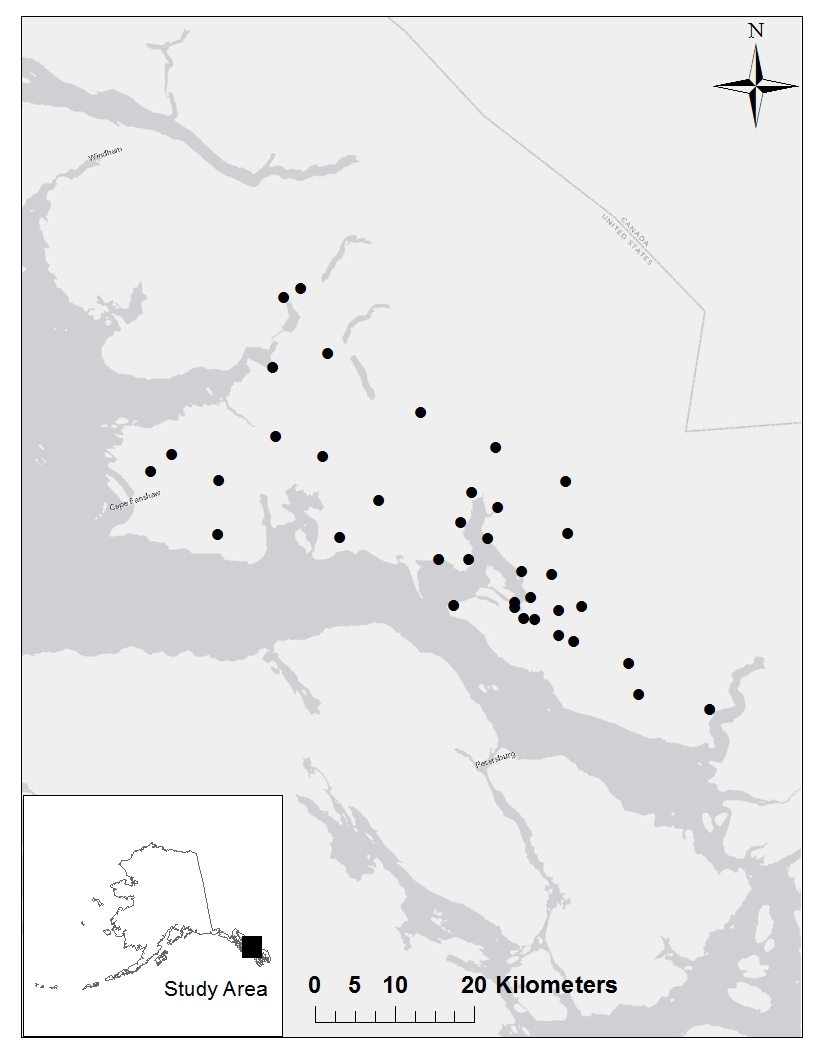
\includegraphics[height=4.22in,width=3.2in]{Ch5-SCR0/figs/Wolverines_cameratrap}
\end{center}
\caption{
Wolverine camera trap locations (black dots) from a study that took
place in SE Alaska. See
\citet{magoun_etal:2011} for details.
}
\label{scr0.fig.wolverinelocs}
\end{figure}


\subsection{Practical data organization}

To carry out an analysis of these data, we require the matrix of trap
coordinates and the encounter history data.  We usually store data in
2 distinct data files which contain all the information needed for an
analysis. These files are
\begin{itemize}
\item[$\bullet$] The encounter data file (EDF) containing a record of which
  traps and when each individual encounter occurred.
\item[$\bullet$] The trap deployment file (TDF) which contains the
  coordinates of each trap, along with information
 indicating which sample
  occasions each trap was operating.
\end{itemize}

{\flushleft \bf Encounter Data File (EDF)} --
We store the encounter data in the
an efficient file format which is easily manipulated in {\bf R} and
easy to create in  Excel and other spreadsheets which are widely used
for data management.
The file
structure is a simple matrix with 4 columns, those being: (1)
\mbox{\tt session ID}: the trap
{\it session} which usually corresponds to a year or a primary period
in the context of a Robust Design situation, but it could also
correspond to a distinct spatial unit (see
Sec. \ref{mle.sec.multisession} and Chapt. \ref{chapt.hscr}).
For a single-year study (as considered here) this
should be an integer  that is constant for all records; (2) \mbox{\tt
  individual ID}: the
individual identity, being an integer from $1$ to $n$ (repeated for
multiple captures of the same individual) indicating which
individual the record (row) of the matrix belongs to; (3) \mbox{\tt
  occasion ID}: The integer sample
occasion which generated the record, and (4) \mbox{\tt trap ID}: the
trap identity, an
integer from 1 to $J$, the number of traps.  The structure of the EDF
is the same as used in the \mbox{\tt secr} package \citep{efford:2011}
and similar to that used
in the {\bf SPACECAP} \citep{gopalaswamy_etal:2012mee}, and
\mbox{\tt SCRbayes} \citep{russell_etal:2012} packages, both of which
have a 3-column format (\mbox{\tt trapID}, \mbox{\tt indID}, \mbox{\tt
  sampID}). We note that the naming of the columns is irrelevant as
far as anything we do in this book, although \mbox{\tt secr} and other
software may have requirements on variable naming. 

To illustrate this format, the wolverine data are available in the
package \mbox{\tt scrbook} by typing:
\begin{verbatim}
data(wolverine)
\end{verbatim}
which contains a list having elements \mbox{\tt wcaps} (the EDF) and
\mbox{\tt wtraps} (the TDF).  We see that \mbox{\tt wcaps} has 115
rows, each representing a unique encounter event including the trap
identity, the individual identity and the sample occasion index
(\mbox{\tt sample}).  The first 5 rows of \mbox{\tt wcaps} are:
{\small
\begin{verbatim}
> wolverine$wcaps[1:5,]
     year individual day trap
[1,]    1          2 127    1
[2,]    1          2 128    1
[3,]    1          2 129    1
[4,]    1         18 130    1
[5,]    1          3 106    2
\end{verbatim}
}
To reiterate the structure, the variable \mbox{\tt year} is in
integer indicating the year or session of the encounter. All these
data come from a single year (2008) and so \mbox{\tt year} is set to
1. Variable \mbox{\tt individual} is an integer identity of each
individual captured, \mbox{\tt day} is the sample occasion of capture
(in this case, the sample occasions correspond to days), and \mbox{\tt
  trap} is the integer trap identity.
Often, the variable \mbox{\tt trapid} will have to
correspond to the row of a matrix containing the trap coordinates - in
this case the TDF file \mbox{\tt wtraps} which we describe further below.

\begin{comment}
{\bf
I THINK WE SHOULD PUT ALL THIS INFO INTO A DATA CLASS WITH SOME
  CONSTRUCTOR FUNCTION. I WILL WORK ON THAT. EDF, TDF + State-space +
  K(reps) + ??? -- "scr" data type.
}
\end{comment}

Note that the information provided in this encounter data file
\mbox{\tt wcaps} does not represent a completely informative summary
of the data. For example, if no individuals were captured in a certain
trap or during a certain period, then this compact data format will
have no record. Thus we will need to know $J$, the number of traps,
{\it and} $K$, the number of sample occasions
when reformatting this SCR data format into a 2-d
encounter frequency matrix or 3-d array. In addition, the encounter
data file does not provide information about which periods each trap
was operated. This additional information is also necessary as the
trap-specific sample sizes must be passed to {\bf BUGS} as data. We
provide this information along with trap
coordinates, in the ``trap deployment file'' (TDF)
 which is described below.

For our purposes we need to convert the \mbox{\tt wcaps} file into the
 $n \times J$ array of
binomial encounter frequencies, although more general models might
require an encounter-history formulation of the model which requires a
full 3-d array.  To obtain our encounter frequency matrix, we do this
the hard way by first converting the encounter data file into a 3-d
array and then summarize to trap totals. We have a handy function
\mbox{\tt SCR23darray} which takes the compact encounter data file,
and
converts it to a 3-d array, and then we use the {\bf R} function
\mbox{\tt apply} to summarize over the sample occasion dimension (by
convention here, this is the 2nd dimension). To apply this to the
wolverine data in order to compute the 3-d array we do this:
{\small
\begin{verbatim}
y3d <- SCR23darray(wolverine$wcaps,wolverine$wtraps)
y <- apply(y3d,c(1,3),sum)
\end{verbatim}
}
See the help file for more information on \mbox{\tt SCR23darray}.
The 3-d array is necessary to fit certain types of models (e.g.,
behavioral response) and this is why we sometimes will require this
maximally informative 3-d data format but, here, we analyze the
summarized data.


{\flushleft \bf Trap Deployment File (TDF)} -- The other important
information needed to fit SCR models is the ``trap deployment file''
(TDF) which provides the additional information not contained in the
encounter data file. The traps file has $K + 3$ columns. The first
column is assumed to be a trap identifier, columns 2 and 3 are the
easting and northing coordinates (assumed to be in a Euclidean
coordinate system), and columns 4 to $K + 3$ are binary indicators of
whether each trap was operational during each sample occasion. The
first 10 rows (out of 37) and 10 columns (out of 167) of the trap
deployment file for the wolverine data are shown as follows:
{\small
\begin{verbatim}
wolverine$wtraps[1:10,1:10]

   Easting Northing 1 2 3 4 5 6 7 8
1   632538  6316012 0 0 0 0 0 0 0 0
2   634822  6316568 1 1 1 1 1 1 1 1
3   638455  6309781 0 0 0 0 0 0 0 0
4   634649  6320016 0 0 0 0 0 0 0 0
5   637738  6313994 0 0 0 0 0 0 0 0
6   625278  6318386 0 0 0 0 0 0 0 0
7   631690  6325157 0 0 0 0 0 0 0 0
8   632631  6316609 0 0 0 0 0 0 0 0
9   631374  6331273 0 0 0 0 0 0 0 0
10  634068  6328575 0 0 0 0 0 0 0 0
\end{verbatim}
}
This tells us that trap 2 was operated in periods (days) 1-7 but the
other traps were not operational during those periods. It is extremely
important to recognize that each trap was operated for a variable
period of time and thus the binomial ``sample size'' is different for
each, and this needs to be accounted for in the {\bf BUGS} model
specification.  To compute the vector of sample sizes $K$, and extract
the trap locations, we do this:
\begin{verbatim}
traps <- wolverine$wtraps
traplocs <- traps[,1:2]
K <- apply(traps[,3:ncol(traps)],1,sum)
\end{verbatim}
This results in a matrix \mbox{\tt traplocs} which contains the
coordinates of each trap and a vector $K$ containing the number of
days that each trap was operational. We now have all the information
required to fit a basic SCR model in {\bf BUGS}.



Summarizing the data for the wolverine study, we see that 21
unique individuals were captured a total of 115 times. Most
individuals were captured 1-6 times, with 4, 1, 4, 3, 1, and 2
individuals captured 1-6 times, respectively.  In addition, 1
individual was captured each 8 and 14 times and 2 individuals each
were captured 10 and 13 times.  The number of unique traps that
captured a particular individual ranged from 1-6, with 5, 10, 3, 1, 1,
and 1 individual captured in each of 1 to 6 different traps, respectively, for a
total of 50 unique wolverine-trap encounters.  These numbers might be
hard to get your mind around whereas some tabular summary is often
more convenient. For that it seems natural to tabulate individuals by
trap and total encounter frequencies. The spatial information in SCR
data is based on multi-trap captures,
%\footnote{I will add more context
%  here on revision about spatial recaptures, lost recaptures, ordinary
%  recaptures. Function \mbox{\tt SCRsmy} in \mbox{\tt scrbook}. {\bf
%    XXXX THIS NEEDS WRITTEN XXXXX}  },
 and so, it is informative to understand how many unique traps each
individual is captured in. At the same time, it is useful to
understand how many total captures we have of each individual because
this is, in an intuitive sense, the effective sample size.  So, we
reproduce Table 1 from \citet{royle_etal:2011jwm} which shows,
in Table \ref{scr0.tab.wolverine}, the trap
and total encounter frequencies.



\begin{table} [htp]
  \caption{Individual frequencies of capture for wolverines captured
    in camera traps in Southeast Alaska in 2008. Rows index unique
    traps of capture for each individual
and columns represent total number of captures
    (e.g., we captured 4 individuals 1 time, necessarily in only 1
    trap; we captured 3 individuals 3 times but in 2 different traps).
%% Kimmy confirmed table is same as in JWM paper
}
\centering
\begin{tabular}{c c c c c c c c c c c}
\hline
 & \multicolumn{10}{c}{No. of captures} \\ \hline
No. of traps & 1 & 2 & 3 & 4 & 5 & 6 & 8 & 10 &13 &14 \\
\hline
1 & 4 & 1 & 0 & 0 & 0 & 0 & 0 & 0 & 0 & 0 \\
2 & 0 & 0 & 3 & 2 & 0 & 2 & 1 & 2 & 0 & 0 \\
3 & 0 & 0 & 1 & 1 & 0 & 0 & 0 & 0 & 0 & 1 \\
4 & 0 & 0 & 0 & 0 & 0 & 0 & 0 & 0 & 1 & 0 \\
5 & 0 & 0 & 0 & 0 & 1 & 0 & 0 & 0 & 0 & 0 \\
6 & 0 & 0 & 0 & 0 & 0 & 0 & 0 & 0 & 1 & 0 \\
\hline
\end{tabular}
\label{scr0.tab.wolverine}
\end{table}


\subsection{Fitting the model in WinBUGS}

For illustrative purposes here we fit the simplest SCR model with the
Gaussian distance function although we revisit these data with more
complex models in later chapters. The model is summarized by the
following 4 elements:
\begin{itemize}
\item[(1)] $y_{ij}|{\bf s}_{i} \sim \mbox{Binomial}(K, z_{i}\; p_{ij})$
\item[(2)] $p_{ij} = p_{0} \exp(-\alpha_{1} \; ||{\bf x}_{j}-{\bf s}_{i}||^2)$
\item[(3)] ${\bf s}_{i} \sim \mbox{Uniform}({\cal S})$
\item[(4)] $z_{i} \sim \mbox{Bernoulli}(\psi)$
\end{itemize}
We assume customary flat priors on the structural (hyper-) parameters
of the model, $\alpha_{0} = \mbox{logit}(p_{0})$, $\alpha_{1}$ and
$\psi$.

It remains to define the
state-space ${\cal S}$. For this, we nested the trap array (Fig.
\ref{scr0.fig.wolverinelocs}) in a
 rectangular state-space extending $20$ km beyond the traps in each cardinal
direction.  We also considered larger state-spaces up to 50 km to
evaluate that choice.  The buffer of the state space should be large
enough so that individuals beyond the state-space boundary are not
likely to be encountered
(Sec. \ref{scr0.sec.ss}).
Thus, some knowledge of typical space usage
patterns of the species is useful to establish the model state-space.  For the analysis,
we scaled the coordinate system
so that a unit distance was equal to $10$ km, producing a rectangular
state-space of dimension $9.88 \times 10.5$ units ($area = 10374$ km$^2$)
within which the trap array was nested. As a general rule, we
recommend scaling the state-space so that it is defined near the
origin $(x,y)=(0,0)$. While the scaling of the coordinate system is
theoretically irrelevant, a poorly scaled coordinate system can
produce Markov chains that mix poorly.  For the scaled coordinate
system we fit models for various choices of a rectangular state-space
based on
buffers from 1.0 to 5.0 units (10 km to
50 km). In the {\bf R} package \mbox{\tt scrbook} we provide a
function
\mbox{\tt wolvSCR0} which will fit the basic SCR model. For
example, to fit the model in
{\bf WinBUGS} using data augmentation with $M=300$ potential individuals,
using 3 Markov chains each of 12000 total iterations, discarding the
first 2000 as burn-in, we execute the following {\bf R} commands:
{\small
\begin{verbatim}
> library(scrbook)
> data(wolverine)
> traps <- wolverine$wtraps
> y3d <- SCR23darray(wolverine$wcaps,wolverine$wtraps)
> toad <- wolvSCR0(y3d,traps,nb=2000,ni=12000,buffer=1,M=300)
\end{verbatim}
}
The argument \mbox{\tt buffer} determines the buffer size of the
state-space.  Note that this analysis takes between 1-2 hours on many
machines (in 2013) 
so we recommend trying it out with lower values of $M$ and
fewer iterations.  The posterior summaries are shown in
Table \ref{scr0.tab.wolverine-results}.


\begin{comment}
\footnote{Final as of 1/11/2012.
output saved in \mbox{\tt wolv-buffer-study.txt}}
\end{comment}

\begin{table}
{\small
\centering
\caption{
Posterior summaries of SCR model parameters for the wolverine camera
trapping data from SE Alaska.
Each analysis was based on 3 chains, 12000 iterations, 2000 burn-in,
for a total of 30000 posterior samples.
}
\begin{tabular}{cllrllrllr}
Buffer &\multicolumn{3}{c}{sigma} & \multicolumn{3}{c}{N} & \multicolumn{3}{c}{D} \\
\hline \hline
   & mean &	sd	&n.eff&	mean &	sd   &n.eff&	mean&	sd&	n.eff \\ \hline
10&	0.65&	0.06&	1800&				39.63&	6.70& 7100&	5.97&	1.00&	7100 \\
15&	0.64&	0.06&	510&				48.77&	9.19&	3300&	5.78&	1.09&	3300\\
20&	0.64&	0.06&	1200&				59.84&	11.89&	20000&	5.77&	1.15&	20000\\
25&	0.64&	0.05&	3600&				72.40&	14.72&	2700&	5.79&	1.18&	2700\\
30&	0.63&	0.05&	5600&				86.42&	17.98&	3900&	5.82&	1.21&	3900\\
35&	0.63&	0.05&	4500&				101.79&	21.54&	30000&	5.85&	1.24&	30000\\
40&	0.64&	0.05&	410&				118.05&	26.17&	410&	5.87&	1.30&	450\\
45&	0.64&	0.05&	10000&				134.43&	28.68&	3300&	5.83&	1.24&	3300\\
50&	0.63&	0.05&	4700&				151.61&	31.65&	3400&	5.79&	1.21&	3400\\
55&	0.64&	0.05&	1600&				169.28&	35.81&
260&	5.73&	1.21&	260\\ \hline
\end{tabular}
}
\label{scr0.tab.wolverine-results}
\end{table}



\begin{comment}
{\small
\begin{verbatim}
All based on 3 chains, 12k iters, 2k burn, 30k total
Buffer = 10 km
           mean    sd   2.5%    25%    50%    75%  97.5% Rhat n.eff
psi        0.13  0.03   0.08   0.11   0.13   0.15   0.20    1 10000
sigma      0.65  0.06   0.55   0.61   0.64   0.68   0.76    1  1800
p0         0.06  0.01   0.04   0.05   0.06   0.06   0.08    1 20000
N         39.63  6.70  29.00  35.00  39.00  44.00  54.00    1  7100
D          5.92  1.00   4.33   5.22   5.82   6.57   8.06    1  7100
alpha1     1.23  0.21   0.85   1.08   1.22   1.36   1.66    1  1800
deviance 410.05 12.06 388.70 401.50 409.20 417.80 435.60    1 22000

Buffer = 15 km
 n.sims = 30000 iterations saved
           mean    sd   2.5%    25%    50%    75%  97.5% Rhat n.eff
psi        0.16  0.04   0.10   0.14   0.16   0.19   0.25    1  3800
sigma      0.64  0.06   0.54   0.60   0.64   0.67   0.76    1   510
p0         0.06  0.01   0.04   0.05   0.06   0.06   0.08    1 17000
N         48.77  9.19  34.00  42.00  48.00  54.00  69.00    1  3300
D          5.78  1.09   4.03   4.98   5.69   6.40   8.18    1  3300
alpha1     1.25  0.21   0.86   1.10   1.24   1.39   1.70    1   510
deviance 411.00 12.16 389.50 402.40 410.30 418.70 437.00    1  5400

Buffer = 20 km
           mean    sd   2.5%    25%    50%    75%  97.5% Rhat n.eff
psi        0.20  0.05   0.12   0.17   0.20   0.23   0.30    1 16000
sigma      0.64  0.06   0.54   0.60   0.63   0.67   0.76    1  1200
p0         0.06  0.01   0.04   0.05   0.06   0.06   0.08    1  1900
N         59.84 11.89  40.00  51.00  59.00  67.00  86.00    1 20000
D          5.77  1.15   3.86   4.92   5.69   6.46   8.29    1 20000
alpha1     1.26  0.21   0.87   1.11   1.25   1.40   1.71    1  1200
deviance 411.01 12.36 389.10 402.30 410.20 418.80 437.50    1  1500

Buffer = 25 km
           mean    sd   2.5%    25%    50%    75%  97.5% Rhat n.eff
psi        0.24  0.05   0.15   0.20   0.24   0.28   0.36    1  3400
sigma      0.64  0.05   0.54   0.60   0.63   0.67   0.75    1  3600
p0         0.06  0.01   0.04   0.05   0.06   0.06   0.08    1  5000
N         72.40 14.72  47.00  62.00  71.00  81.00 105.00    1  2700
D          5.79  1.18   3.76   4.96   5.67   6.47   8.39    1  2700
alpha1     1.26  0.21   0.88   1.12   1.25   1.40   1.71    1  3600
deviance 411.35 12.23 389.70 402.70 410.55 419.20 437.20    1 30000

Buffer = 30 km
           mean    sd   2.5%    25%    50%    75%  97.5% Rhat n.eff
psi        0.29  0.06   0.18   0.24   0.28   0.33   0.43    1  3100
sigma      0.63  0.05   0.54   0.60   0.63   0.67   0.75    1  5600
p0         0.06  0.01   0.04   0.05   0.06   0.06   0.08    1 11000
N         86.42 17.98  56.00  74.00  85.00  97.00 126.02    1  3900
D          5.82  1.21   3.77   4.98   5.72   6.53   8.49    1  3900
alpha1     1.27  0.21   0.88   1.12   1.26   1.41   1.71    1  5600
deviance 411.06 12.37 389.20 402.50 410.20 418.90 437.60    1 10000

Buffer = 35 km
           mean    sd   2.5%    25%    50%    75%  97.5% Rhat n.eff
psi        0.34  0.08   0.21   0.29   0.34   0.39   0.50    1 30000
sigma      0.63  0.05   0.54   0.60   0.63   0.67   0.75    1  4500
p0         0.06  0.01   0.04   0.05   0.06   0.06   0.08    1 24000
N        101.79 21.54  65.00  87.00 100.00 115.00 148.00    1 30000
D          5.85  1.24   3.74   5.00   5.75   6.61   8.51    1 30000
alpha1     1.27  0.21   0.89   1.12   1.25   1.40   1.70    1  4500
deviance 411.10 12.20 389.50 402.40 410.30 418.90 437.20    1 22000

Buffer = 40 km
           mean    sd   2.5%    25%    50%    75%  97.5% Rhat n.eff
psi        0.39  0.09   0.24   0.33   0.39   0.45   0.60 1.01   480
sigma      0.64  0.05   0.54   0.60   0.63   0.67   0.75 1.01   410
p0         0.06  0.01   0.04   0.05   0.06   0.06   0.08 1.00 21000
N        118.05 26.14  75.00 100.00 116.00 133.00 178.00 1.01   450
D          5.87  1.30   3.73   4.97   5.76   6.61   8.84 1.01   450
alpha1     1.27  0.21   0.89   1.12   1.25   1.40   1.72 1.01   410
deviance 411.37 12.35 389.30 402.60 410.60 419.30 437.50 1.00  9700

Buffer = 45 km
           mean    sd   2.5%    25%    50%    75%  97.5% Rhat n.eff
psi        0.45  0.10   0.28   0.38   0.44   0.51   0.66    1  3600
sigma      0.64  0.05   0.54   0.60   0.63   0.67   0.75    1 10000
p0         0.06  0.01   0.04   0.05   0.06   0.06   0.08    1  8100
N        134.43 28.68  85.00 114.00 132.00 153.00 196.00    1  3300
D          5.83  1.24   3.68   4.94   5.72   6.63   8.50    1  3300
alpha1     1.26  0.21   0.88   1.11   1.24   1.39   1.69    1 10000
deviance 411.36 12.19 389.60 402.70 410.60 419.10 437.30    1  9400

Buffer = 50 km
           mean    sd   2.5%    25%    50%    75%  97.5% Rhat n.eff
psi        0.51  0.11   0.31   0.43   0.50   0.57   0.74    1  3200
sigma      0.63  0.05   0.54   0.60   0.63   0.67   0.75    1  4700
p0         0.06  0.01   0.04   0.05   0.06   0.06   0.08    1  3300
N        151.61 31.65  96.00 129.00 149.00 172.00 221.00    1  3400
D          5.79  1.21   3.66   4.92   5.69   6.56   8.43    1  3400
alpha1     1.27  0.21   0.89   1.12   1.25   1.40   1.70    1  4700
deviance 410.81 12.18 389.20 402.30 410.10 418.50 436.70    1 30000

Buffer = 55 km
           mean    sd   2.5%    25%    50%    75%  97.5% Rhat n.eff
psi        0.56  0.12   0.35   0.48   0.55   0.64   0.82 1.01   260
sigma      0.64  0.05   0.54   0.60   0.63   0.67   0.76 1.00  1600
p0         0.06  0.01   0.04   0.05   0.06   0.06   0.08 1.00 30000
N        169.28 35.81 108.00 143.00 166.00 192.00 247.00 1.01   260
D          5.73  1.21   3.66   4.84   5.62   6.50   8.36 1.01   260
alpha1     1.25  0.21   0.88   1.11   1.24   1.39   1.69 1.00  1600
deviance 411.28 12.38 389.40 402.60 410.50 419.10 437.50 1.00 26000
\end{verbatim}
}
\end{comment}


% XXXX It would be nice to remind people what the posterior summaries
% mean. i.e what does the 2.5 percentile tell us? XXXX

\subsection{Summary of the wolverine analysis}

We see that the estimated density is roughly consistent as we increase
the state-space buffer from $15$ to $55$ km. We do note that the data
augmentation parameter $\psi$ (and, correspondingly, $N$) increase with
the size of the state space in accordance with the deterministic
relationship $N= D*A$. However, density is more or less constant as we
increase the size of the state-space beyond a certain point.  For the
10 km state-space buffer, we see a slight effect on the posterior
distribution of $D$ because the state-space is not sufficiently large.
The full results from the analysis based on 20 km state-space buffer
are given in Table \ref{scr0.tab.wolverine-results2}.

\begin{table}
\centering
\caption{
Posterior summaries of SCR model parameters for the wolverine camera
trapping data from SE Alaska. The model was run with the trap array
centered in a state-space with a $20$ km
rectangular buffer.
}
\begin{tabular}{crrrrrrrc}
\hline \hline
parameter & mean & SD & 2.5\% & 25\% & 50\% & 75\% & 97.5\% &\mbox{\tt
  Rhat}  \\
\hline
$\psi$  &      0.20&  0.05&   0.12&   0.17&   0.20&   0.23&   0.30 &   1 \\
$\alpha_1$ &     1.26&  0.21&   0.87&   1.11&   1.25&   1.40&   1.71 &   1 \\
$\sigma$&      0.64&  0.06&   0.54&   0.60&   0.63&   0.67&   0.76 &   1 \\
$p_0$   &      0.06&  0.01&   0.04&   0.05&   0.06&   0.06&   0.08 &   1 \\
$N$    &     59.84& 11.89&  40.00&  51.00&  59.00&  67.00&  86.00 &   1 \\
$D$    &      5.77&  1.15&   3.86&   4.92&   5.69&   6.46&   8.29 &
1 \\ \hline
\end{tabular}
\label{scr0.tab.wolverine-results2}
\end{table}

Our point estimate of wolverine density from this study, using the
posterior mean from the state-space based on the 20 km buffer, is
approximately $5.77$ individuals/1000 km$^2$ with a 95\% posterior
interval of $[3.86, 8.29]$. Density is estimated imprecisely which
might not be surprising given the low sample size ($n=21$
individuals!). This seems to be a basic feature of carnivore studies
although it should not (in our view) preclude the study of their
populations by capture-recapture nor attempts to estimate density or vital rates.


It is worth thinking about this model, and these estimates, computed
under a rectangular state space roughly centered over the trapping
array (Fig. \ref{scr0.fig.wolverinelocs}).  Does it make sense to
define the state-space to include, for example, ocean? What are the
possible consequences of this? What can we do about it?  There's no
reason at all that the state space has to be a regular polygon -- we
defined it as such here strictly for convenience and for ease of
implementation in {\bf WinBUGS} where it enables us to specify the
prior for the activity centers as uniform priors for each coordinate.
While it would be possible to define a more realistic state-space
using some general polygon GIS coverage, it might take some effort to
implement that in the {\bf BUGS} language but it is not difficult to
devise custom MCMC algorithms to do that (see
Chapt. \ref{chapt.mcmc}).  Alternatively, we recommend using a
discrete representation of the state-space -- i.e., approximate ${\cal
  S}$ by a grid of $G$ points. We discuss this in Sec.
\ref{scr0.sec.discrete}.

\subsection{Wolverine space usage}

The parameter $\alpha_{1}$ is related to the home range radius
(Sec. \ref{scr0.sec.implied}).  For the Gaussian kernel model we
interpret the scale parameter $\sigma$, related to $\alpha_1$ by
$\alpha_1 = 1/(2\sigma^2)$, as the radius of a bivariate normal model
of space usage.  In this case $\sigma = 0.64$ standardized units ($10$
km), which corresponds to $0.64 \times 10 = 6.4$ km.  It can be
argued then that 95\% of space used by an individual is within $6.4
\mbox{km} \times \sqrt{5.99} = 15.66$ km of the home range center. The
effective ``home range area'' is then the area of this circle, which is
$\pi \times 15.66^2 = 770.4$ $\mbox{km}^{2}$
Using our handy function \mbox{\tt hra} we do this:
\begin{verbatim}
 hra(pGauss1,parms=c(-2,1/(2*.64*.64)),xlim=c(-1,7),ylim=c(-1,7))

[1] 7.731408
\end{verbatim}
which is in units of 100 km$^2$, so 773.1. The difference in this case
is due to numerical approximation of our all-purpose tool \mbox{\tt
  hra}. This home range size is
relatively huge for measured home ranges, which range between
100 and 535 km$^2$ \citep{whitman_etal:1986}.

\citet{royle_etal:2011jwm} reported estimates for $\sigma$ in the
range
$6.3-9.8$
km depending on the model, which isn't too different than
here\footnote{ \citet{royle_etal:2011jwm} expressed the model as
  $\mbox{cloglog}(p_{ij}) = \alpha_{0} - (1/\sigma^2)*d_{ij}^2$, but
  the estimates of $\sigma$ reported in their Table 2 are actually
  based on the model according to $\mbox{cloglog}(p_{ij}) = \alpha_{0}
  - \frac{1}{2\sigma^{2}}*d_{ij}^2$, and so the estimates of $\sigma$
  they report in units of km are consistent to what we report here
  except based on the complementary log-log link instead (Gaussian
  hazard) of the Gaussian encounter probability model. }.  However,
these estimates are larger than the typical home range sizes suggested
in the literature.  One possible explanation is that if a wolverine is
using traps as a way to get yummy chicken, so it's moving from trap to
trap instead of adhering to ``normal'' space usage patterns, then the
implied home range size might not be worth much biologically.  Thus,
interpretation of detection models in terms of home range area depends
on some additional context or assumptions, such as that traps don't
effect individual space usage patterns. As such, we caution against
direct biological interpretations of home range area based on
$\sigma$, although SCR models can be extended to handle more general,
non-Euclidean, patterns of space usage. See Chapts.~\ref{chapt.ecoldist}
and \ref{chapt.rsf}.

We can calibrate the desired size of the state-space by looking at the
estimated home range radius of the species. We should target a buffer
of width $2-3 \times \sigma$ in order that the probability of
encountering an individual is very close to 0 beyond the prescribed
state-space. Essentially, by specifying a state-space, we're setting
$p=0$ for individuals beyond the prescribed state-space. For the
wolverine data, with $\sigma$ in the range of 6-9 km, a state-space
buffer of 20 km is sufficiently large.


\section{Using a Discrete Habitat Mask}
\label{scr0.sec.discrete}

The SCR model developed previously in this chapter assumes that
individual activity centers are distributed uniformly over the
prescribed state-space. Clearly this will not always be a reasonable
assumption. In Chapt. \ref{chapt.state-space} we talk about developing
models that allow explicitly for non-uniformity of the activity
centers by modeling covariate effects on density. A simplistic method
of
affecting the distribution of activity centers, which we address here,
is to modify the shape and organization of the state-space
explicitly. For example, we might be able to classify the state-space
into distinct blocks of habitat and non-habitat. In that case we can
remove the non-habitat from the state-space and assume uniformity of
the activity centers over the remaining portions judged to be suitable
habitat.  There are several ways to approach this: We can use a
 grid of points to represent the state-space, i.e., by the set
of coordinates ${\bf s}_1, \ldots, {\bf s}_{G}$, and assign equal
probabilities to each possible value. Alternatively, we can retain the
continuous formulation of the state-space but attempt to describe
constraints analytically, or we can use polygon clipping methods to
enforce constraints on the state-space in the MCMC analysis. We focus
here on the formulation of the basic SCR model in terms of a discrete
state-space but in Chapt. \ref{chapt.mcmc}
we demonstrate the latter approach based on using polygon
operations to define an irregular state-space.
Use of a discrete state-space can be computationally expensive in {\bf
  WinBUGS}. That said, it isn't too difficult to perform the MCMC
calculations in {\bf R} (discussed in Chapt.
\ref{chapt.mcmc}). The {\bf R} package {\tt SPACECAP}
\citep{gopalaswamy_etal:2012mee} arose from the {\bf R} implementation of
the SCR model in \citet{royle_etal:2009ecol}.
%As we will see in
%Chapt. \ref{chapt.mle}, we must prescribe the state-space by a
%discrete mesh of points in order to do integrated likelihood and so if
%we are using a discrete state-space this can be accommodated directly
%in our code for obtaining MLEs.

While clipping out non-habitat seems like a good idea, we think
investigators should go about this very cautiously.  We might prefer
to do it when non-habitat represents a clear-cut restriction on the
state-space such as a reserve boundary or a lake, ocean or river. But,
having the capability to do this also causes people to start defining
``habitat'' vs. ``non-habitat'' based on their understanding of the
system whereas it can't be known whether the animal being studied has
the same understanding.  Moreover, differentiating the landscape by
habitat or habitat quality must affect the geometry and morphology of
home ranges (see Chapt. \ref{chapt.rsf}) much more so than the
plausible locations of activity centers. That is, a home range
centroid could, in actual fact, occur in a shopping mall parking lot if
there is pretty good habitat around the shopping mall, so there is probably no
sense preclude it as the location for
an activity center.  It would generally be better to include some
definition of habitat quality in the model for the detection
probability \citep{royle_etal:2012ecol} which we address in
Chapts. \ref{chapt.rsf} and \ref{chapt.ecoldist}.


\subsection{Evaluation of coarseness of habitat mask}

The coarseness of the state-space should not really have much of an
effect on estimates if the grain is sufficiently fine relative to
typical animal home range sizes.  Why is this?  We have two analogies
that can help us understand. First is the relationship to model
$M_{h}$.  As noted in Sec. \ref{scr0.sec.scrmh} above, we can think
about SCR models as a type of finite mixture
\citep{norris_pollock:1996, pledger:2000} where we are fortunate to be
able to obtain direct information about which group individuals belong
to (group being location of activity center).  In the standard finite
mixture models we typically find that a small number of groups (e.g.,
2 or 3 at the most) can explain  high levels of heterogeneity
and are adequate for most data sets of small to moderate sample
sizes. We therefore expect a similar effect in SCR models when we
discretize the state-space.  We can also think about discretizing the
state-space as being related to numerical integration where we find
(see Chapt. \ref{chapt.mle}) that we don't need a very fine grid of
support points to evaluate the integral to a reasonable level of
accuracy. We demonstrate this here by reanalyzing simulated data using
a state-space defined by a different number of support points.  We
provide an {\bf R} script called \mbox{\tt SCR0bayesDss} in the
{\bf R} package \mbox{\tt scrbook}.  We note that for this comparison
we generated the actual activity centers as a continuous random
variable and thus the discrete state-space is, strictly speaking, an
approximation to truth. That said, we regard all state-space
specifications as approximations to truth in the sense that they
represent a component of the SCR model.
% Thus the use of any specific
%discrete state-space is not intrinsically more ``wrong'' than any
%specific continuous representation.
% XXXX Hmmm, I'm not sure I buy this last sentence. XXXX
%%% Fair enough

As with our {\bf R} function \mbox{\tt SCR0bayes}, the modification
\mbox{\tt SCR0bayesDss} will use either {\bf WinBUGS} or {\bf
  JAGS}. In addition, it requires a grid resolution argument
(\mbox{\tt ng}) which is the dimension of 1 side of a square state-space.
To execute this function we do, for example:
{\small
\begin{verbatim}
> library(scrbook)
> data <- simSCR0(discard0=TRUE,rnd=2013)   # generate data set

# run with JAGS
> out1 <- SCR0bayesDss(data,ng=8,M=200,engine="jags",ni=2000,nb=1000)

# run with WinBUGS
> out2 <- SCR0bayesDss(data,ng=8,M=200,engine="winbugs",ni=2000,nb=1000)
\end{verbatim}
}
We fit this model to the same simulated data set for $6 \times 6$,
$9 \times 9$, $12 \times 12$, $15\times 15$ state-space grids.  For
{\bf WinBUGS}, we used 3 chains of 5000 total length with 1000
burn-in, which yields 12000 total posterior samples.  Summary results
are shown in Table \ref{scr0.tab.discrete}.  The results are broadly
consistent except for the $6\times 6$ case.  We see that the run time
increases with the size of the state-space grid (not unexpected), such
that we imagine it would be impractical to run models with more than a
few hundred state-space grid points.  We found (not shown here) that
the runtime of {\bf JAGS} is much faster and, furthermore, relatively
{\it constant} as we increase the grid size.  We suspect that {\bf
  WinBUGS} is evaluating the full-conditional for each activity center
at all $G$ possible values whereas it may be that {\bf JAGS} is
evaluating the full-conditional only at a subset of values or perhaps
using previous calculations more effectively.  While this might
suggest that one should always use {\bf JAGS} for this analysis, we
found in our analysis of the wolverine (next section) that {\bf JAGS}
could be extremely sensitive to starting values, producing MCMC
algorithms that often simply do not work for some problems, so be
careful when using {\bf JAGS}. To improve its performance, always
start the latent activity centers at values near where individuals
were captured.
The performance of either should improve if we compute the full
distance matrix outside of {\bf BUGS} and pass it as data, although we
haven't fully evaluated this approach.



\begin{table}
\centering
\caption{
Comparison of the
effect of state-space grid coarseness on estimates of $N$ for a
simulated data set. Posterior
summaries and run time are given. Results obtained  using
{\bf WinBUGS} run from {\tt R2WinBUGS}.
}
\begin{tabular}{crrrrrrrc} \hline \hline
grid  & Mean & SD &   NaiveSE & Time-seriesSE &  runtime (sec) \\ \hline
6     &    111.6699& 16.61414& 0.1516657 &  0.682008 &     2274 \\
9     &    114.2294& 17.99109& 0.1642355 &  0.833291 &    4300 \\
12    &    115.9806& 17.3843 & 0.1586964 &  0.762756 &    7100 \\
15    &    115.379 & 17.93721& 0.1637436 &  0.832483 &   13010 \\
\hline
\end{tabular}
\label{scr0.tab.discrete}
\end{table}


\begin{comment}
\begin{verbatim}
Table XYZ.Effect of grid coarseness on estimates of N using JAGS and
WinBUGS.

$I would only show results from one engine. COuld simply say in the text that WB was about 5x slower$
JAGS run from rjags
             Mean       SD    NaiveSE  Time-seriesSE  runtime
6    N     109.7717 15.98959 0.0923160    0.377737    1239
9    N     114.4621 16.72025 0.0965344    0.468659    1267
12   N     115.4309 17.12403 0.098866     0.464830    1576
15   N     114.7699 17.0242  0.0982894    0.425238    1638
20   N     116.0370 17.10686 0.0987665    0.486867    1647
25   N     116.3228 16.98323 0.0980527    0.465527    1661
30   N     116.4252 17.4078  0.100504     0.533735    1806
WinBUGS run from R2WinBUGS
             Mean       SD    NaiveSE  Time-seriesSE  runtime
6    N     111.6699 16.61414 0.1516657   0.682008     2274
9    N     114.2294 17.99109 0.1642355   0.833291     4300
12   N     115.9806 17.3843  0.1586964   0.762756     7100
15   N     115.379  17.93721 0.1637436   0.832483    13010

Note: WinBUGS based on fewer samples too!
\end{verbatim}
\end{comment}



\subsection{Analysis of the wolverine camera trapping data}
\label{scr0.sec.wolvgrid}

We reanalyzed the wolverine data using discrete state-space grids with
points spaced by 2, 4 and 8 km (see
Fig. \ref{scr0.fig.wolvgrids}). These were constructed from a 40 km
buffered state-space, and deleting the points over water
\citep[see][]{royle_etal:2011jwm}.  Our interest in doing this was to
evaluate the relative influence of grid resolution on estimated
density because the coarser grids will be more efficient from a
computational stand-point and so we would prefer to use them, but
only if there is no strong influence on estimated density.
The posterior summaries  for the 3 habitat grids are given in Table \ref{scr0.tab.wolvgrids}.
We see that the density estimates are quite a bit larger than obtained in our
analysis
(Table \ref{scr0.tab.wolverine-results})
based on a rectangular, continuous state-space.
We also see that there are slight differences depending on the
resolution of the state-space grid.
Interestingly, the
effectiveness of the MCMC algorithms, as measured by effective sample
size (\mbox{\tt n.eff}) is pretty remarkably
different. Furthermore, the finest grid resolution ($2$ km spacing) took about
6 days to run and thus it would not be practical for large problems or
with many models.

\begin{figure}[ht]
\begin{center}
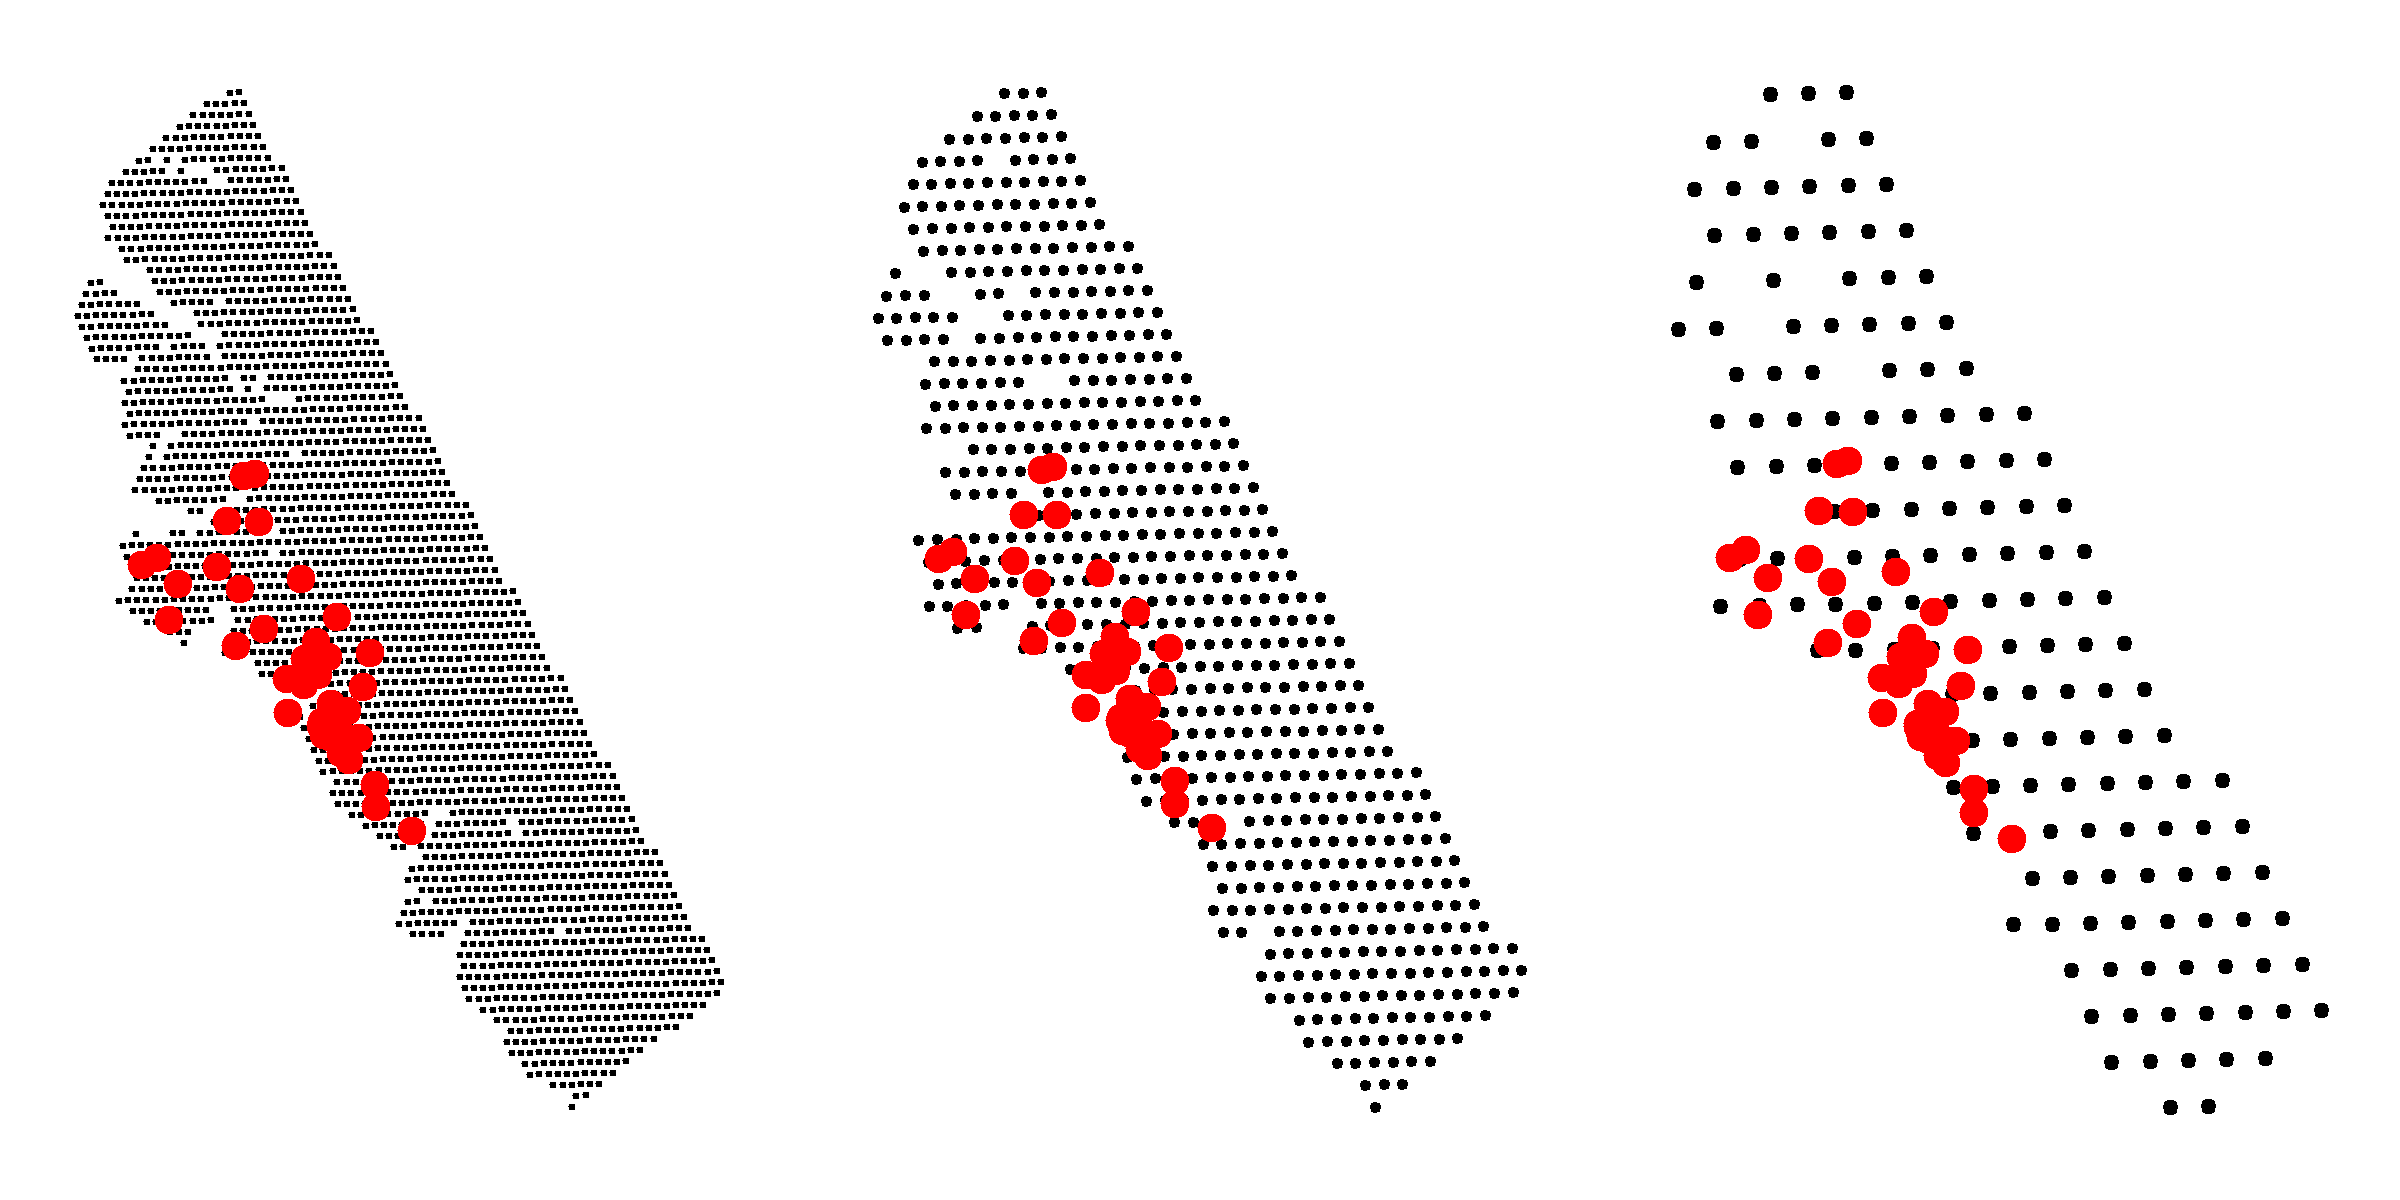
\includegraphics[height=2.5in,width=5in]{Ch5-SCR0/figs/wolvgrids}
\end{center}
\caption{Three habitat mask grids used in the comparison of the effect of pixel size on the estimated
  density surface of wolverines.  The 3 cases are
2 (left), 4 (center) and 8 (right) km spacing of state-space points, extending
40 km from the vicinity of the trap array. }
\label{scr0.fig.wolvgrids}
\end{figure}

%% KIMMY PUT THESE IN TABLE
%%  Insert in comment before editing

\begin{table}[ht]
\centering
\caption{
Posterior summaries for the wolverine camera trapping data, using
model SCR0, with a Gaussian hazard encounter probability model, and a discrete habitat mask of 3 different resolutions: 2,
4 and 8 km. Parameters are $\lambda_{0}$ = baseline encounter rate,
$p_{0} = 1-\exp(-\lambda_{0})$, $\sigma$ is the scale parameter of the
Gaussian kernel, $\psi$ is the data augmentation parameter, $N$ and
$D$ are population size and density, respectively.
Models fitted using {\bf WinBUGS}, 
  3 chains, each with 11000 iterations (first 1000 discarded)
producing  30000 posterior samples. 
}
\begin{tabular}{l r r r r r r r r r}
  \hline \hline
  2km spacing & & & & & & & & &\\
  \hline
  &   mean &   sd &  2.5\% &  25\% &  50\% &  75\% &  97.5\% &  Rhat &
  n.eff \\ \hline
  $\sigma$ &  0.62 &  0.05 &  0.54 &  0.59 &  0.62 &  0.65 &  0.73 &  1.01 &  160 \\
  $\lambda_0$ & 0.05 & 0.01 &  0.04 &  0.04 &  0.05 &  0.06 & 0.07 &  1.01 & 320 \\
  $p_0$  &  0.05 &  0.01 & 0.03 & 0.04 & 0.05 & 0.05 &  0.06 & 1.01 & 320 \\
  $\psi$ &   0.43 &  0.09 &  0.27 &  0.37 &  0.43 &  0.49  &  0.63 &  1.00 &  560 \\
  N & 86.56 & 16.94 & 57.00 & 75.00 & 85.00 & 97.00 & 124.00 & 1.00 & 510 \\
  D & 8.78 &  1.72 & 5.78 & 7.60 & 8.62 & 9.83 & 12.57 & 1.00 & 510 \\
  \hline
  4km spacing & & & & & & & & &\\
  \hline
  &   mean &   sd &  2.5\% &  25\% &  50\% &  75\% &  97.5\% &  Rhat &
  n.eff \\ \hline
  $\sigma$ & 0.61 & 0.04 & 0.53 & 0.58 & 0.61 &  0.64 &  0.71 &   1 & 1600 \\
  $\lambda_0$ &  0.05 & 0.01 & 0.04 & 0.05 & 0.05 &  0.06 &  0.07 &   1 & 2500 \\
  $p_0$  &   0.05 & 0.01 & 0.03 & 0.04 & 0.05 &  0.05 &  0.07 &   1 & 2500 \\
  $\psi$ &   0.45 & 0.09 & 0.28 & 0.38 & 0.44 &  0.50 &  0.64 &   1 & 1300 \\
  N  &   89.25 & 17.44 &  59.00 & 77.00 & 88.00 & 100.00 & 127.00  &  1 & 1100 \\
  D  &    9.01 & 1.76 & 5.96 & 7.77 & 8.88 & 10.10 & 12.82  &  1 & 1100 \\
  \hline
  8km spacing & & & & & & & & &\\
  \hline
  &   mean &   sd &  2.5\% &  25\% &  50\% &  75\% &  97.5\% &  Rhat &
  n.eff \\ \hline 
  $\sigma$ & 0.68 & 0.05 & 0.59 & 0.64 & 0.67 & 0.71 &  0.77 & 1.01 &  220 \\
  $\lambda_0$ &  0.05 & 0.01 & 0.03 & 0.04 & 0.05 & 0.05 &  0.06 & 1.00 &  560 \\
  $p_0$  &   0.05 & 0.01 & 0.03 & 0.04 & 0.04 & 0.05 &  0.06 & 1.00 &  560 \\
  $\psi$  &  0.42 & 0.09 & 0.26 & 0.36 & 0.41 & 0.47 &  0.61 & 1.00 &  940 \\
  N  &   83.18 & 16.14 & 56.00 & 72.00 & 82.00 & 93.00 & 119.00 & 1.00 &  700 \\
  D   &   8.28 & 1.61 & 5.57 & 7.17 & 8.16 & 9.26 & 11.84 & 1.00 &  700 \\
  \hline
\end{tabular}
\label{scr0.tab.wolvgrids}
\end{table}


\begin{comment}
{\small
\begin{verbatim}
> print(out.2km,digits=2)
Inference for Bugs model at "modelfile.txt", fit using WinBUGS,
 3 chains, each with 11000 iterations (first 1000 discarded)
 n.sims = 30000 iterations saved
       mean    sd  2.5%   25%   50%   75%  97.5% Rhat n.eff
psi    0.43  0.09  0.27  0.37  0.43  0.49   0.63 1.00   560
sigma  0.62  0.05  0.54  0.59  0.62  0.65   0.73 1.01   160
lam0   0.05  0.01  0.04  0.04  0.05  0.06   0.07 1.01   320
p0     0.05  0.01  0.03  0.04  0.05  0.05   0.06 1.01   320
N     86.56 16.94 57.00 75.00 85.00 97.00 124.00 1.00   510
D      8.78  1.72  5.78  7.60  8.62  9.83  12.57 1.00   510

> print(out.4km,digits=2)
Inference for Bugs model at "modelfile.txt", fit using WinBUGS,
 3 chains, each with 11000 iterations (first 1000 discarded)
 n.sims = 30000 iterations saved
       mean    sd  2.5%   25%   50%    75%  97.5% Rhat n.eff
psi    0.45  0.09  0.28  0.38  0.44   0.50   0.64    1  1300
sigma  0.61  0.04  0.53  0.58  0.61   0.64   0.71    1  1600
lam0   0.05  0.01  0.04  0.05  0.05   0.06   0.07    1  2500
p0     0.05  0.01  0.03  0.04  0.05   0.05   0.07    1  2500
N     89.25 17.44 59.00 77.00 88.00 100.00 127.00    1  1100
D      9.01  1.76  5.96  7.77  8.88  10.10  12.82    1  1100

> print(out.8km,digits=2)
Inference for Bugs model at "modelfile.txt", fit using WinBUGS,
 3 chains, each with 11000 iterations (first 1000 discarded)
 n.sims = 30000 iterations saved
       mean    sd  2.5%   25%   50%   75%  97.5% Rhat n.eff
psi    0.42  0.09  0.26  0.36  0.41  0.47   0.61 1.00   940
sigma  0.68  0.05  0.59  0.64  0.67  0.71   0.77 1.01   220
lam0   0.05  0.01  0.03  0.04  0.05  0.05   0.06 1.00   560
p0     0.05  0.01  0.03  0.04  0.04  0.05   0.06 1.00   560
N     83.18 16.14 56.00 72.00 82.00 93.00 119.00 1.00   700
D      8.28  1.61  5.57  7.17  8.16  9.26  11.84 1.00   700

For each parameter, n.eff is a crude measure of effective sample size,
and Rhat is the potential scale reduction factor (at convergence, Rhat=1).
\end{verbatim}
}
\end{comment}


\begin{comment}
We did the analysis in JAGS also. The results are shown below. {\bf Note}: I
am going to run these again but for longer to finalize the results.

{\small
\begin{verbatim}
 ### 01/10/2012 -- need to rerun these JAGS runs but use more
iterations and check results.


2km
Iterations = 7001:13000
Thinning interval = 1
Number of chains = 3
Sample size per chain = 6000

          Mean        SD  Naive SE Time-series SE
N     86.28522 16.950626 1.263e-01      0.4878973
lam0   0.04807  0.007512 5.599e-05      0.0002199
p0     0.04581  0.006820 5.083e-05      0.0001996
psi    0.28904  0.062117 4.630e-04      0.0017481
sigma  0.62769  0.043596 3.249e-04      0.0018724

4km
          Mean        SD  Naive SE Time-series SE
N     85.53139 16.998966 1.267e-01      0.5181297
lam0   0.04636  0.007542 5.621e-05      0.0002382
p0     0.04425  0.006867 5.118e-05      0.0002172
psi    0.28650  0.061922 4.615e-04      0.0018276
sigma  0.64281  0.048321 3.602e-04      0.0022911

8km
          Mean        SD  Naive SE Time-series SE
N     83.97039 16.508146 1.230e-01      0.4548782
lam0   0.04519  0.006919 5.157e-05      0.0001738
p0     0.04319  0.006319 4.710e-05      0.0001589
psi    0.28146  0.060653 4.521e-04      0.0016555
sigma  0.66956  0.040989 3.055e-04      0.0015070
\end{verbatim}
}
\end{comment}


\section{Summarizing Density and Activity Center Locations}

One of the most useful aspects of SCR models is that they are
parameterized in terms of individual locations -- i.e., {\it where}
each individual lives -- and, thus, we can compute many useful and
interesting summaries of the activity centers obtained from an MCMC
simulation, including maps of density (the number of activity centers
per unit area), estimates of $N$ for any well-defined polygon, or
estimates of where the activity centers for specific individuals
reside. In Bayesian analysis, obtaining such summaries entails no
added calculations,
 when we do analysis by MCMC, because we need only
post-process the output for the individual activity centers to obtain
the desired summaries. We demonstrate that in this section.
Note that you have to be sure to
retain the MCMC history for the ${\bf s}$
variables and also the data augmentation variables z in order to do
some of the following analyses.



\subsection{Constructing density maps}
\label{scr0.sec.mapping}

Because SCR models are spatially-explicit, it is natural to want to
summarize the results of fitting a model by producing a map of
density.  Using Bayesian analysis by MCMC, it is most easy to make a
map of {\it realized} density.  We can do this by tallying up the
number of activity centers ${\bf s}_{i}$ in pixels of arbitrary size
and then producing a nice multi-color spatial plot of the result.
Specifically, let $B({\bf x})$ indicate a pixel centered at ${\bf x}$
then
\[
N({\bf x})=\sum_{i=1}^{M} I({\bf s}_{i} \in B({\bf x}))
\]
(here, $I(arg)$ is the indicator function which evaluates to 1 if
$arg$ is true, and 0 otherwise)
is the population size of pixel  $B({\bf x})$, and $D({\bf x}) = N({\bf
  x})/||B({\bf x})||$ is the local density.
Note that these $N({\bf x})$ parameter are just ``derived
parameters'' as we normally obtain from posterior output using the
appropriate Monte Carlo average (see Chapt.  \ref{chapt.glms}).
% XXXX Another good time to discuss realized vs expected N (or D) and
% reference the recent Efford and Fewster paper. XXXX

One thing to be careful about, in the context of models in which $N$
is unknown, is that, for each MCMC iteration $m$, we only tabulate
those activity centers which correspond to individuals in the sampled
population, i.e., for which the data augmentation variable $z_{i} =
1$.  In this case, we take all of the output for MCMC iterations
$m=1,2,\ldots,\mbox{\tt niter}$ and compute this summary:
\[
   N({\bf x},m) = \sum_{i: z_{i,m}=1} I({\bf s}_{i,m} \in B({\bf x}))
\]
Thus, $N({\bf x},1),N({\bf x},2),\dots,$ is the Markov chain for
parameter $N({\bf x})$.  In what follows we will provide a set of {\bf
  R} commands for doing this calculation and making a basic image
plot from the MCMC output.

{\flushleft \bf Step 1:} Define the center points of each pixel $B({\bf
  x})$, or point at which local density will be estimated:
\begin{verbatim}
> xg <- seq(xlim[1],xlim[2],,50)
> yg <- seq(ylim[1],ylim[2],,50)
\end{verbatim}

{\flushleft \bf Step 2:} Extract the MCMC histories for the activity
centers and the data augmentation variables.  Note that these are each
$N \times \mbox{\tt niter}$ matrices. Here we do this assuming that
{\bf WinBUGS} was run producing the {\bf R} object named \mbox{\tt out}:
\begin{verbatim}
> Sxout <- out$sims.list$s[,,1]
> Syout <- out$sims.list$s[,,2]
> z <- out$sims.list$z
\end{verbatim}

{\flushleft \bf Step 3:} We associate each coordinate with the proper
pixel using the {\bf R} command \mbox{\tt cut()}. Note that we keep only
the activity centers for which $z=1$ (i.e., individuals that belong to
the population of size $N$):
\begin{verbatim}
> Sxout <- cut(Sxout[z==1],breaks=xg,include.lowest=TRUE)
> Syout <- cut(Syout[z==1],breaks=yg,include.lowest=TRUE)
\end{verbatim}

{\flushleft \bf Step 4:} Use the \mbox{\tt table()} command to tally
up how many activity centers are in each $B({\bf x})$:
\begin{verbatim}
> Dn <- table(Sxout,Syout)
\end{verbatim}

{\flushleft \bf Step 5:} Use the \mbox{\tt image()} command to display
the resulting matrix.
\begin{verbatim}
> image(xg,yg,Dn/nrow(z),col=terrain.colors(10))
\end{verbatim}

It is worth emphasizing here that density maps will not usually appear
uniform despite that we have assumed that activity centers are
uniformly distributed. This is because the observed encounters of
individuals provide direct information about the location of the
$i=1,2,\ldots,n$ activity centers and thus their ``estimated''
locations will be affected by the observations. In a limiting sense,
were we to sample space intensely enough, every individual would be
captured a number of times and we would have considerable information
about all $N$ point locations. Consequently, the uniform prior would
have almost no influence at all on the estimated density surface in
this limiting situation. Thus, in practice, the influence of the
uniformity assumption decreases as the fraction of the population
encountered, and the total number of encounters per individual, increases.

{\bf On the non-intuitiveness of \mbox{\tt image()} } -- the {\bf R}
function \mbox{\tt image()}, invoked for a matrix $M$ by \mbox{\tt image(M)}, might
not be very intuitive to some -- it plots $M[1,1]$ in the lower left
corner. If you want $M[]$ to be plotted ``as
you look at it'' then $M[1,1]$ should be in the upper left corner.  We
have a function \mbox{\tt rot()} which does that. If you do \mbox{\tt image(rot(M))} then it
puts it on the monitor as if it was a map you were looking at.  You
can always specify the $x$ and $y-$ labels explicitly as we did above.

{\bf Spatial dot plots } -- A cruder version of the density map can be
made using our
``spatial dot map'' function \mbox{\tt spatial.plot} (in
\mbox{\tt scrbook}).
This function requires, as input, point
locations and the value to be displayed. A simplified
version of this function is as follows:
\begin{verbatim}
> spatial.plot <- function(x,y){
 nc <- as.numeric(cut(y,20))
 plot(x,pch=" ")
 points(x,pch=20,col=topo.colors(20)[nc],cex=2)
 image.scale(y,col=topo.colors(20))
 }
#
# To execute the function do this:
#
> spatial.plot(cbind(xg,yg), Dn/nrow(z))
\end{verbatim}

\subsection{Example: Wolverine density map}

We return to the wolverine study which took place in 2008 in SE Alaska
(Fig. \ref{scr0.fig.wolverinelocs}) and we produce a density map of
wolverines from that analysis. We include the function \mbox{\tt
  SCRdensity} which requires a specific data structure as shown
below. In particular, we have to package up the MCMC history for the
activity centers and the data augmentation variables $z$ into a
list. This also requires that we add those variables to the
parameters-to-be-monitored list when we pass things to {\bf BUGS}.

We used the posterior output from the wolverine model fitted
previously to compute a relatively coarse version of a density map,
using 100 pixels in a $10 \times 10$ grid (Fig. \ref{scr0.fig.density}
top panel) and using 900 pixels arranged in a $30 \times 30$ grid
(Fig. \ref{scr0.fig.density} lower panel) for a fine-scale map. The
{\bf R} commands for producing such a plot (for a short MCMC run) are as
follows:
{\small
\begin{verbatim}
> library(scrbook)
> data(wolverine)
> traps <- wolverine$wtraps
> y3d <- SCR23darray(wolverine$wcaps,wolverine$wtraps)

# this takes 341 seconds on a standard CPU circa 2011
> out <- wolvSCR0(y3d,traps,nb=1000,ni=2000,buffer=1,M=100,keepz=TRUE)

> Sx <- out$sims.list$s[,,1]
> Sy <- out$sims.list$s[,,2]
> z  <- out$sims.list$z
> obj <- list(Sx=Sx,Sy=Sy,z=z)
> tmp <- SCRdensity(obj,nx=10,ny=10,scalein=100,scaleout=100)
\end{verbatim}
In these figures density is
expressed in units of individuals per $100$ km$^2$, while the area of
the pixels is about 103.7 $km^2$ and 11.5 km$^2$, respectively. That
calculation is based on:
\begin{verbatim}
> total.area <- (ylim[2]-ylim[1])*(xlim[2]-xlim[1])*100
> total.area/(10*10)
[1] 103.7427
> total.area/(30*30)
[1] 11.52697
\end{verbatim}
%The {\bf R} commands for producing density maps from MCMC output of
%spatial capture-recapture models is provided in the {\bf R} function
%\mbox{\tt SCRdensity} in the package \mbox{\tt scrbook}.

A couple of things are worth noting: First is that as we move away
from ``where the data live'' -- away from the trap array -- we see
that the density approaches the mean density. This is a property of
the estimator as long as the detection function decreases sufficiently
rapidly as a function of distance.  Relatedly, it is also a property
of statistical smoothers such as splines, kernel smoothers, and
regression smoothers -- predictions tend toward the global mean as the
influence of data diminishes.  Another way to think of it is that it
is a consequence of the prior -- which imposes uniformity, and as you
get far away from the data, the predictions tend to the expected
constant density under the prior.  The other thing to note about this
map is that density is not $0$ over water (although the coastline is
not shown). This might be perplexing to some who are fairly certain
that wolverines do not like water. However, there is nothing about the
model that recognizes water from non-water and so the model predicts
over water {\it as if} it were habitat similar to that within which
the array is nested. But, all of this is OK as far as estimating
density goes and, furthermore, we can compute valid estimates of $N$
over any well-defined region which presumably wouldn't include water
if we so wished. Alternatively, areas covered by water could be masked
out, which we discuss in the next section.

\begin{figure}
\begin{center}
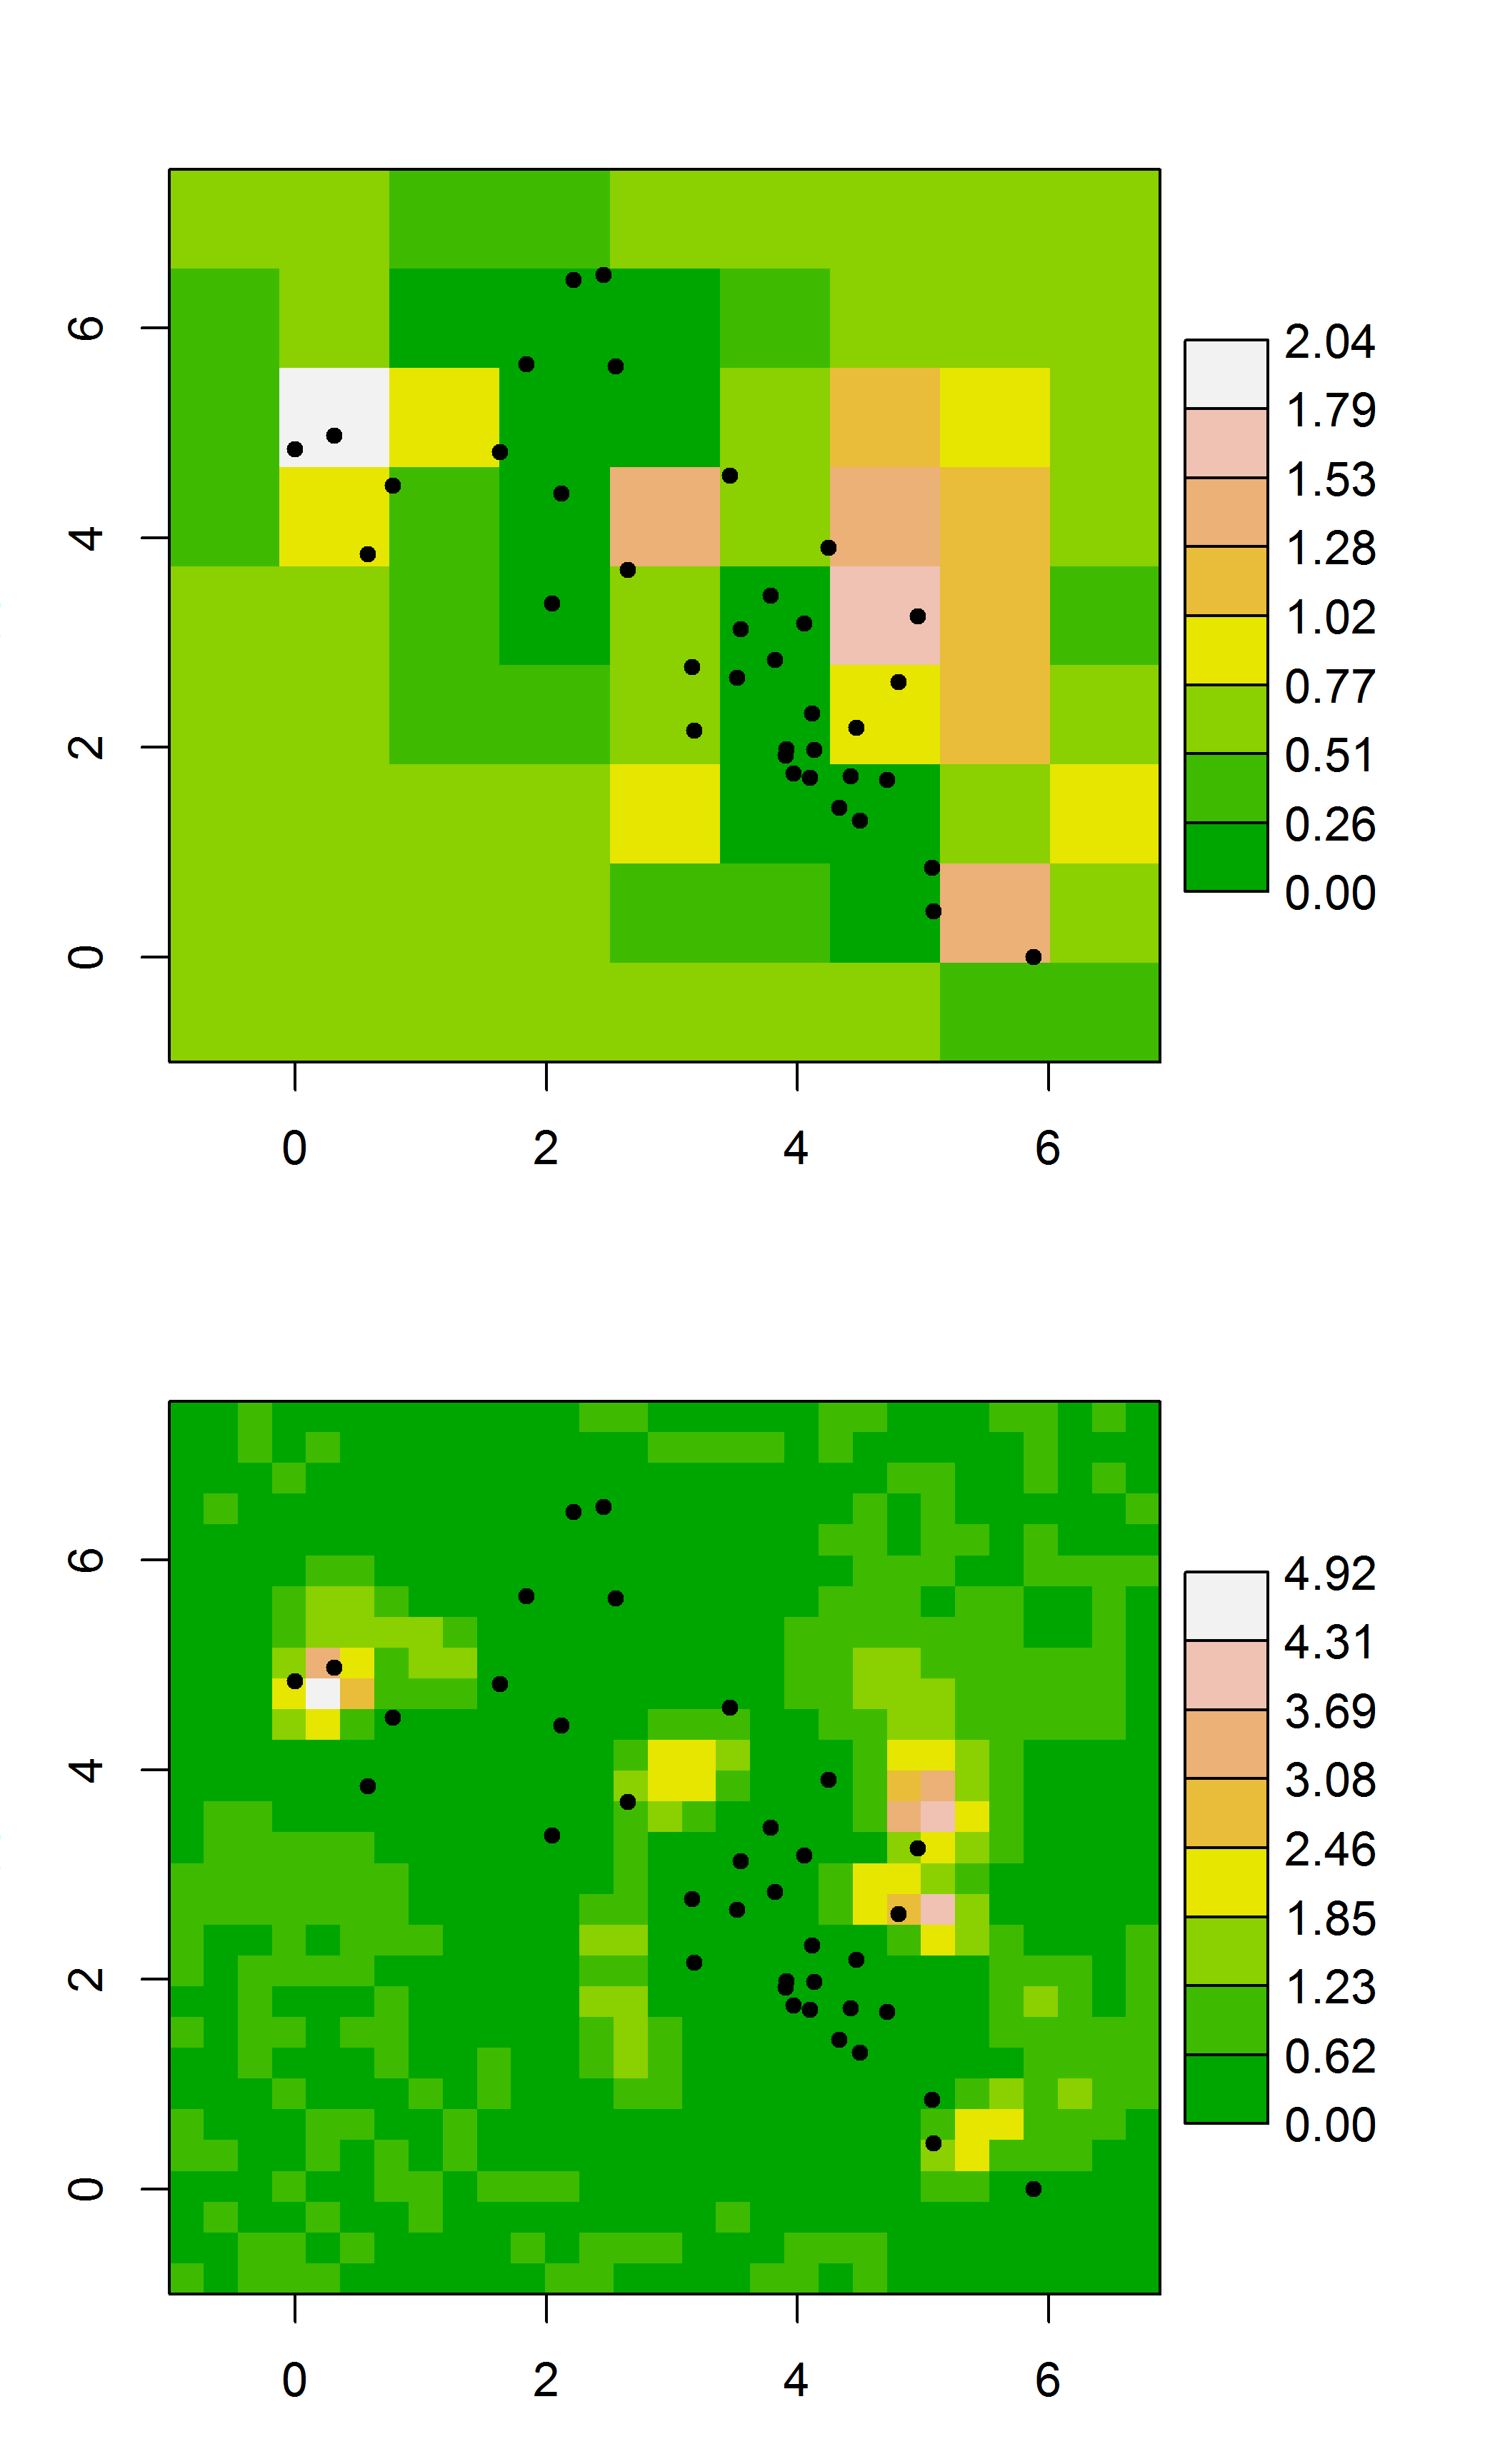
\includegraphics[height=5.75in,width=3.5in]{Ch5-SCR0/figs/wolvDensity}
\end{center}
\caption{Density of wolverines (individuals per 100 km$^2$) in SE Alaska in 2007 based on
  model SCR0. Map grid cells are about 103.7 km$^2$ (top panel) and
11.5 km$^2$ (bottom panel) in area. Dots are the trap locations.}
\label{scr0.fig.density}
\end{figure}



\begin{comment}
\begin{figure}
\begin{center}
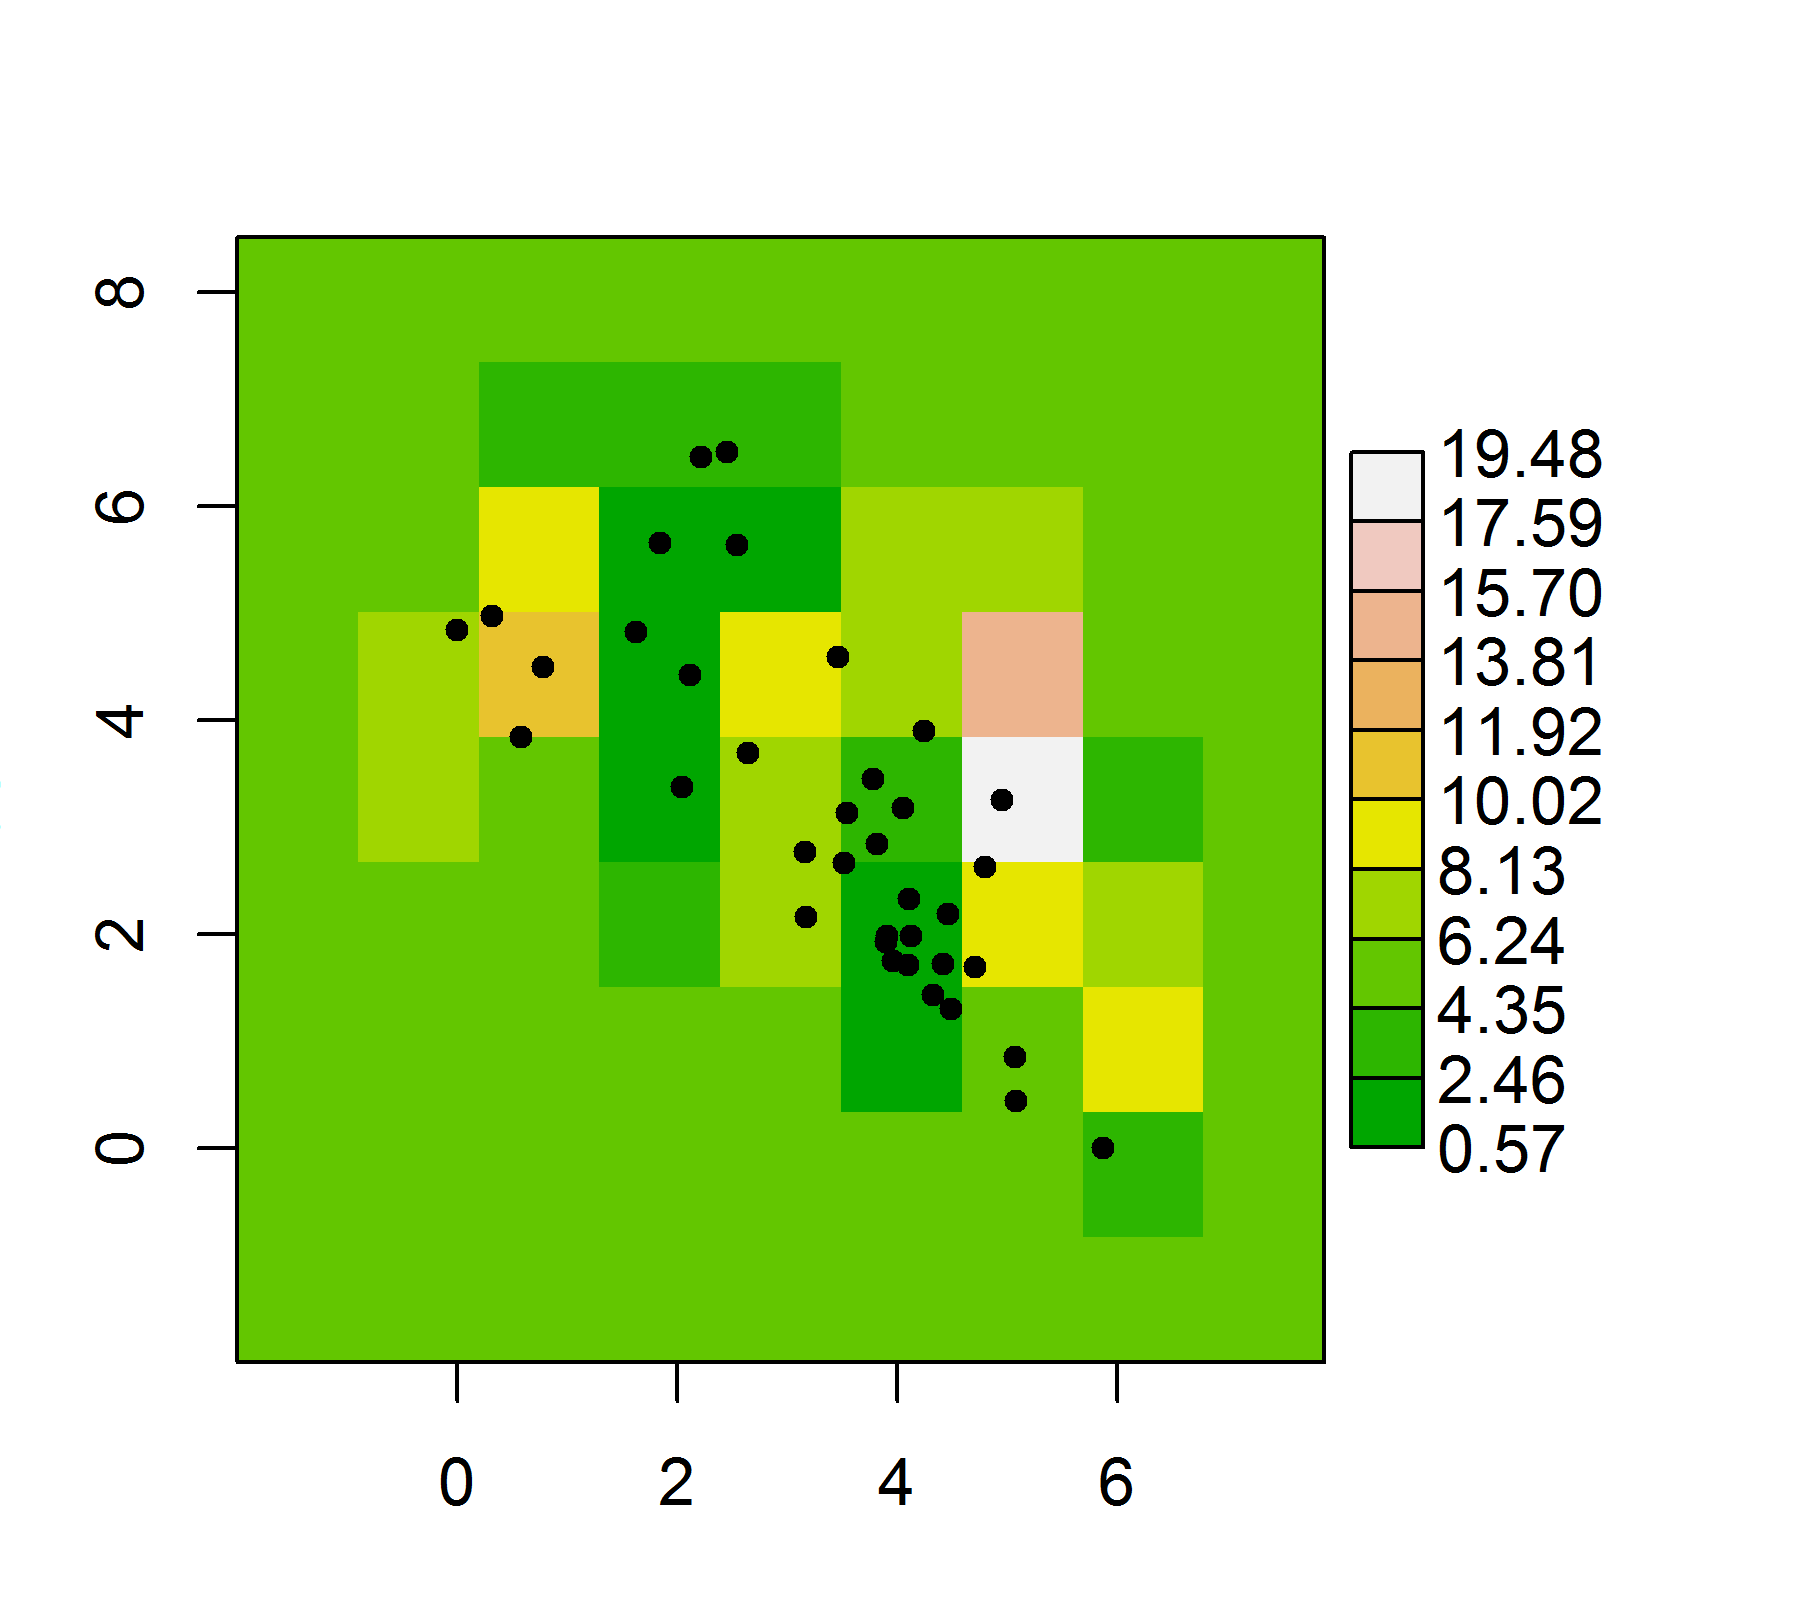
\includegraphics[height=3in,width=3.375in]{Ch5-SCR0/figs/density10x10}
\end{center}
\caption{Density of wolverines (individuals per 100 km$^2$) in SE
  Alaska in 2007 based on model SCR0. Map grid cells are about 103.7
  km$^2$ in area. Dots are the estimated activity centers of the
  observed individuals.}
\label{scr0.fig.density10x10}
\end{figure}

\begin{figure}
\begin{center}
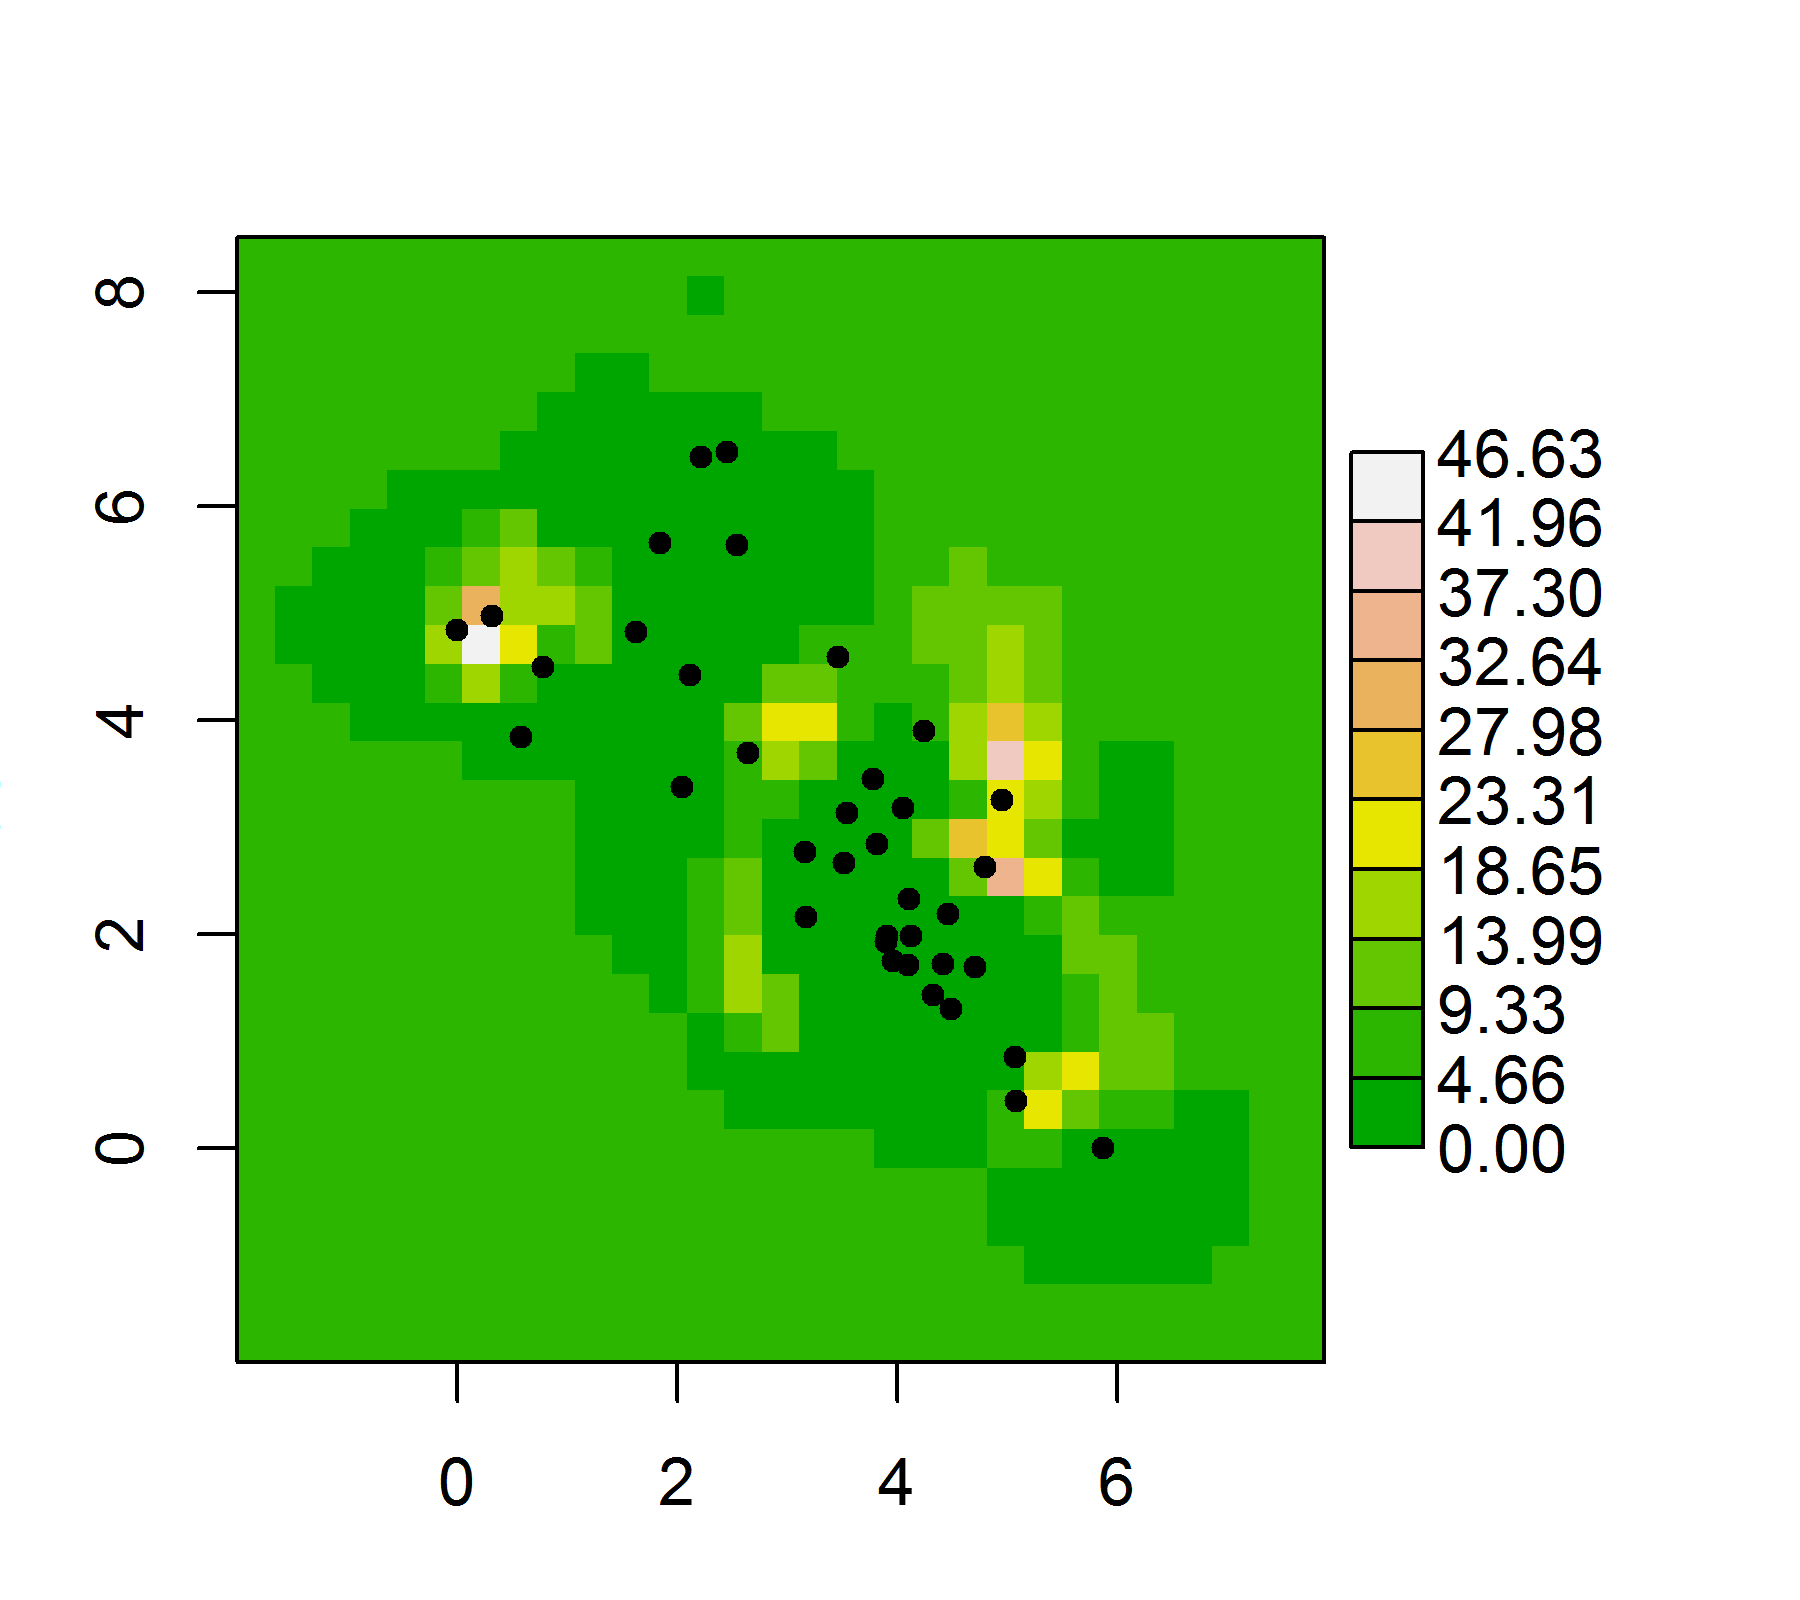
\includegraphics[height=3in,width=3.375in]{Ch5-SCR0/figs/density30x30}
\end{center}
\caption{Density of wolverines (individuals per 100 km$^2$) based on
  model SCR0. Map grid cells are about 11.5 km$^2$.
\label{scr0.fig.density20x20}
\end{figure}
\end{comment}


\subsection{Predicting  where an individual lives}
\label{scr0.sec.post_s}

The density maps in the previous section show the expected number of
individuals per unit area.  A closely related problem is that of
producing a map of the probable location of a specific individual's
activity center.  For any observed encounter history, we can easily
generate a posterior distribution of ${\bf s}_{i}$ for individual $i$.
In addition, for an individual that is {\it not} captured, we can use
the MCMC output to produce a corresponding plot of where such an
individual might live, say ${\bf s}_{n+1}$.  Obviously, all such
uncaptured individuals (for $i=n+1,\ldots,N$) should have the same
posterior distribution.  To illustrate, we show the posterior
distribution of ${\bf s}_{1}$, the activity center for the individual
labeled 1 in the data set, in Fig. \ref{scr0.fig.guy1}. This
individual was captured a single time at trap 30 which is circled in
Fig. \ref{scr0.fig.guy1}.  We see that the posterior distribution is
affected by traps of capture {\it and} traps of non-capture in fairly
intuitive ways.  In particular, because there are other traps in close
proximity to trap 30 which individual 1 was {\it not} captured, the
model pushes it's activity center away from the trap array.  The help
file for \mbox{\tt SCRdensity} shows how to calculate
Fig. \ref{scr0.fig.guy1}.


\begin{figure}[ht]
\begin{center}
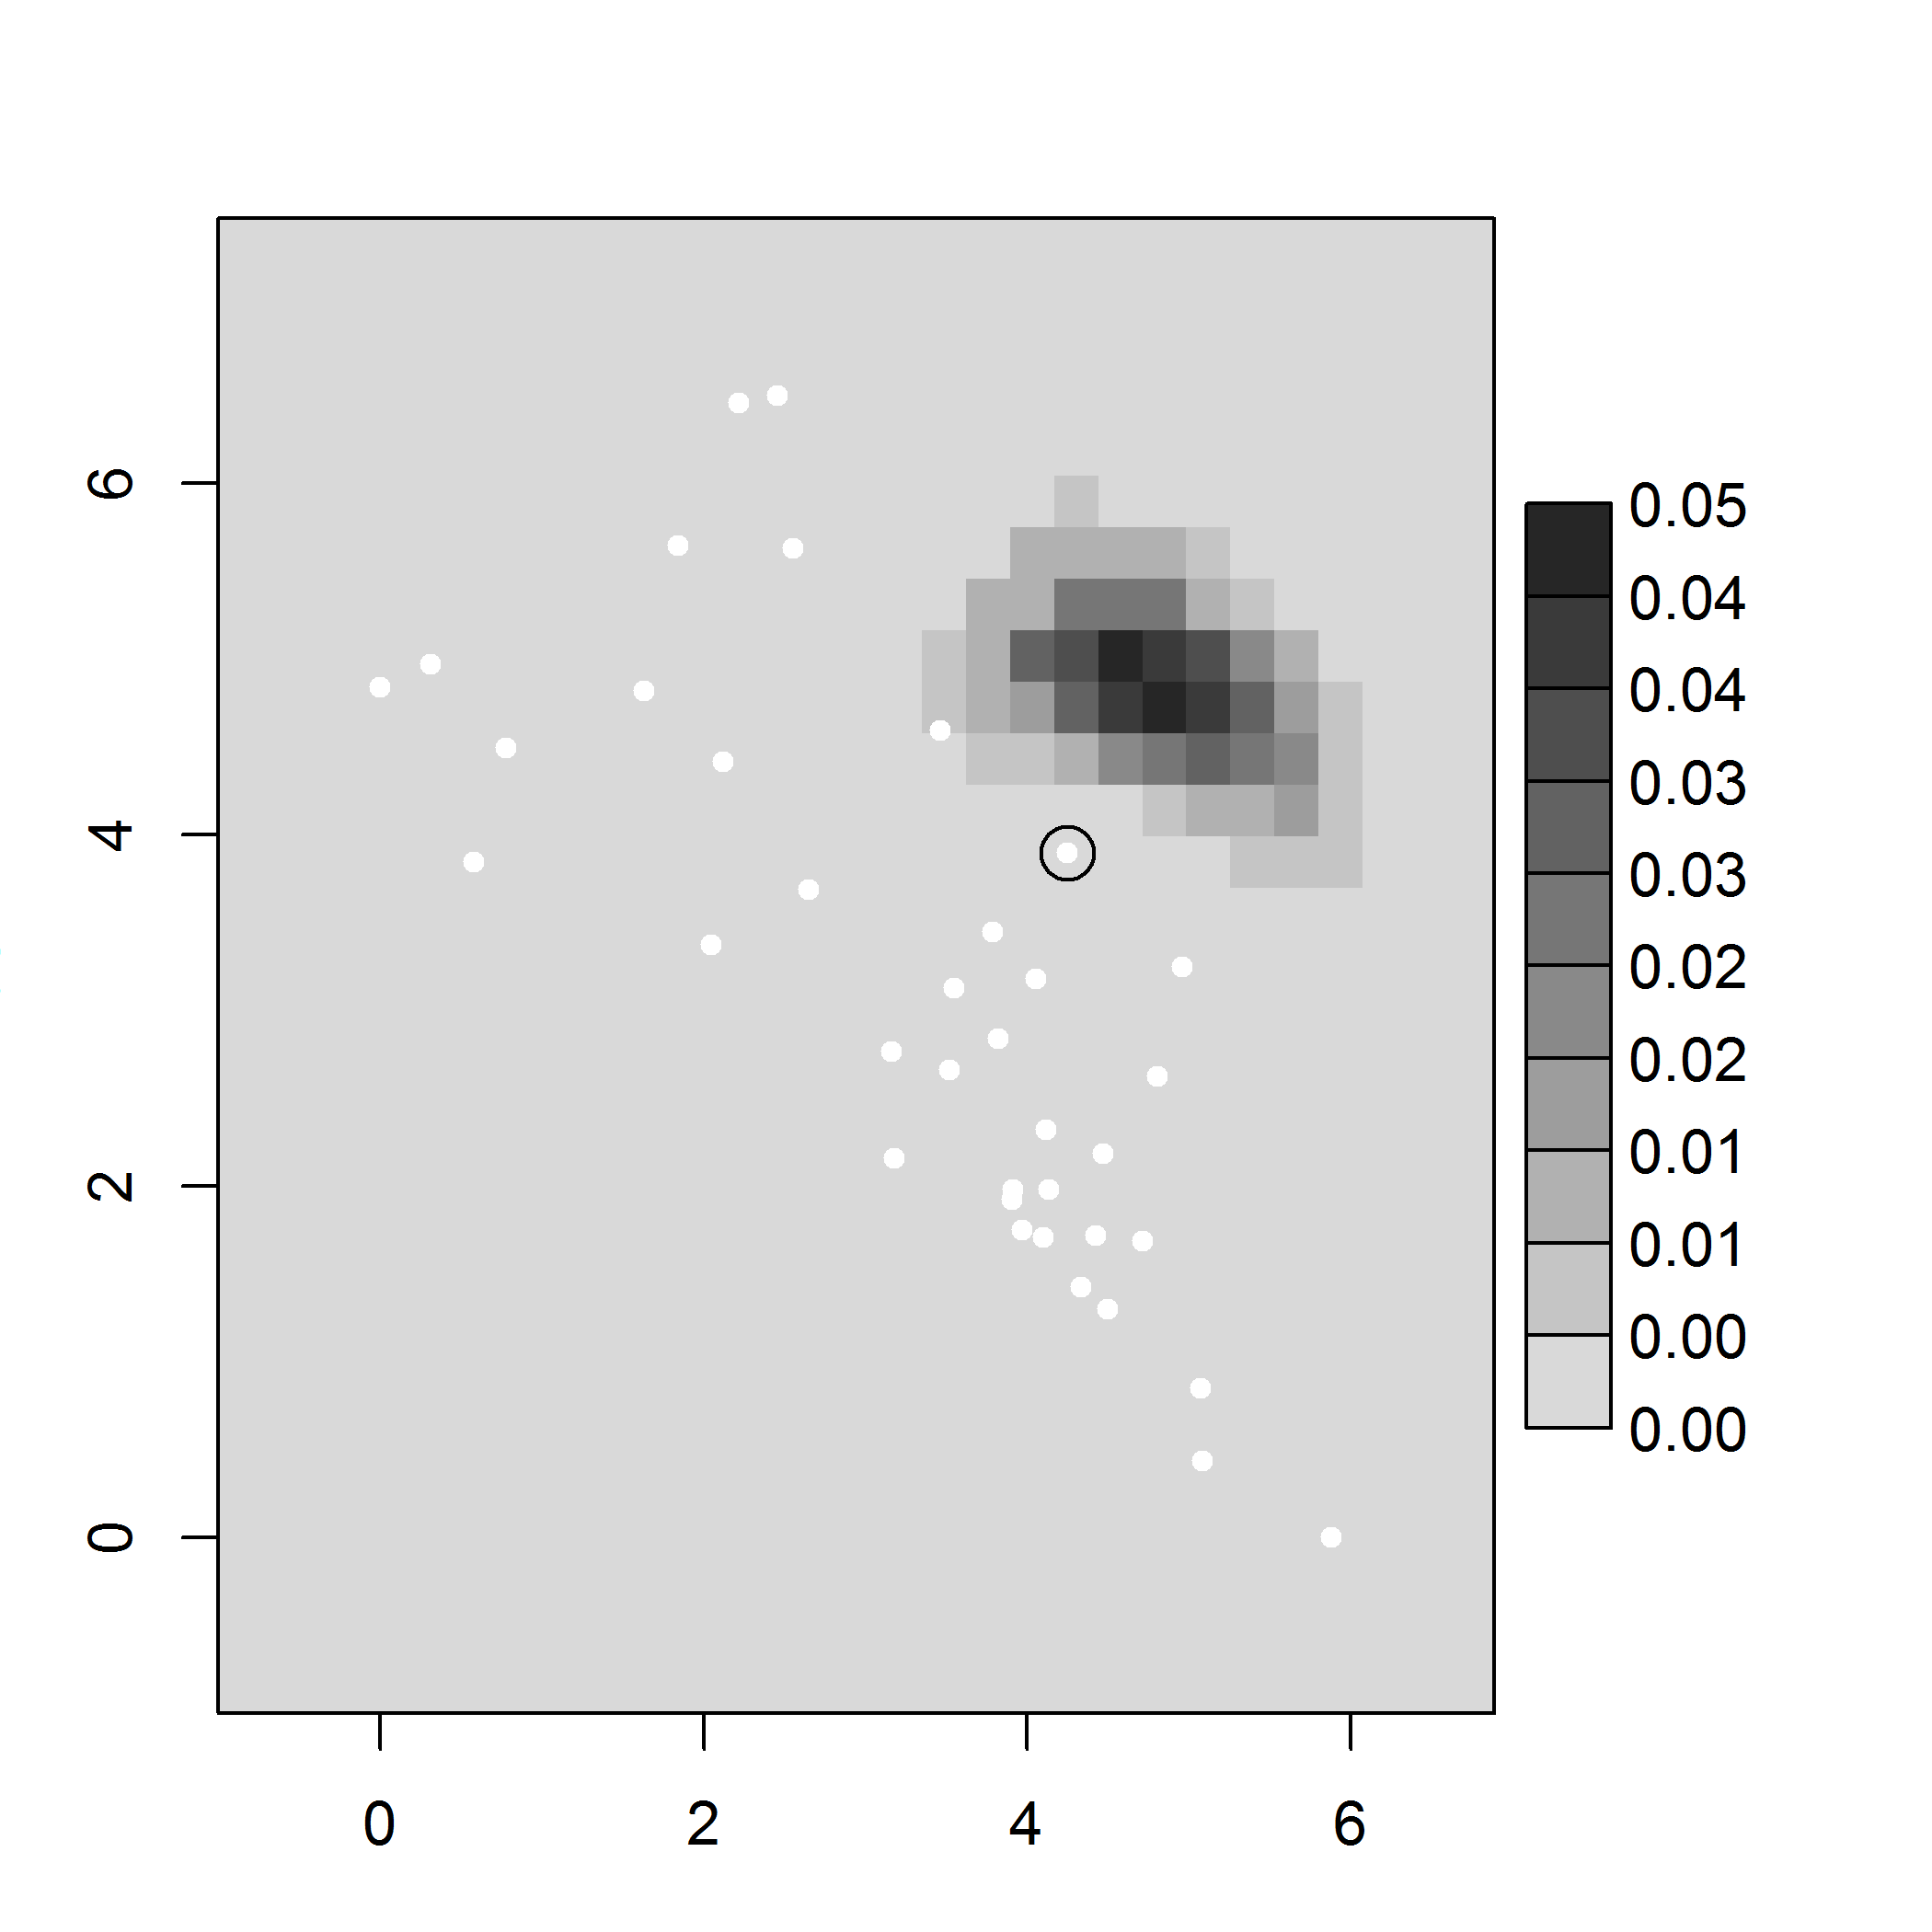
\includegraphics[height=4.25in,width=4.25in]{Ch5-SCR0/figs/wolv_post_s}
\end{center}
\caption{
Posterior probability distribution of ${\bf s}_{1}$, the activity
center for individual 1 in the wolverine data set. This individual was
captured a single time in one trap (trap 30) which is circled. White
dots are trap locations.
}
\label{scr0.fig.guy1}
\end{figure}


\section{Effective Sample Area}
\label{scr0.sec.esa}


\begin{comment}
(1) I think the most general definition of ESA is ESA = \int_S D(x)p(x) where D(x) is the point process intensity at x and p(x) is the capture prob at x. Do you agree with this?


(2) I like your explanation of ESA, but I think we need to note that your formulation assumes that density is constant (a homogeneous point process) such that D = D(x). Also, I think we need to address whether D is the realized D or the expected D. I think it should be the latter, right? So would we defined E[D] = E[N] / Area(S) = (M*phi) / Area(S) ?
\end{comment}


One of the key issues in using ordinary capture recapture models which
we've brought up over and over again is this issue that the area which
is sampled by a trapping array is unknown -- in other words, the $N$
that is estimated by capture-recapture models does not have an
explicit region of space associated with it.  Classically this has
been addressed in the ad hoc way of prescribing an area that contains
the trap array,  usually by adding a buffer of some width, which is not
estimated as part of the capture-recapture model.  In SCR models we
avoid the problem of not having an explicit linkage between $N$ and
``area'', by prescribing explicitly the area within which the
underlying point process is defined -- the state-space of the point
process.  This state-space is {\it not} the ``effective sampled area'' (ESA)
-- it is desirable that it be somewhat larger than the ESA, whatever
that may be, in the sense
that individuals at the edge of the state-space have no probability of
being captured, but as part of the SCR model we don't need to try to
estimate or otherwise characterize the ESA explicitly.

However, it is possible to provide a characterization of effective
sampled area under any SCR model.  This is directly analogous to the
calculation of ``effective strip width'' in distance sampling
\citep{buckland_etal:2001, borchers_etal:2002}.  The conceptual
definition of ESA follows from equating density to ``apparent
density'' -- ESA is the magic number that satisfies that equivalence:
\[
 D = N/A   = n/ESA
\]
In other words, the ratio of $N$ to the area of the state-space should be
equal to the ratio of the observed sample size $n$ to this
number
ESA. Both of these should equal density.
So, to compute ESA for a model, we  substitute $\mathbb{E}(n)$ for $n$
into the above equation, and solve for $ESA$, to get:
\[
 ESA = \mathbb{E}(n)/D.
\]
Our following development assumes that $D$ is constant, but these
calculations can be generalized to allow for $D$ to vary spatially.
% XXXX Shouldn't D be E[D]? Where E[D]=E[N]/Area? I think we also need
% to note that your development assumes that D is constant. Would be
% good show more general definition of ESA too, ie ESA = \int_S
% D(x)p(x), and perhaps reference the IPP chapter. XXXX
%These are good points. You can do this with N/A or E[N]/A it doesn't matter
% -- one is realized, the other is expected. Right?
% About D(x) -- I agree. We could have that generality. But is it necessary?
Imagine our habitat mask for the wolverine data, or the bins we just
used to produce a density map, then we can write $\mathbb{E}(n)$
according to
\[
\mathbb{E}(n) = \sum_{s}  \Pr(\mbox{encounter} | {\bf s}) \mathbb{E}(N({\bf s}) )
\]
where if we prefer to think of this more conceptually we could replace
the summation with an integration (which, in practice, we would just
replace with a summation, and so we just begin there).
In this expression note that
$\mathbb{E}(N({\bf s}))$ is the expected population size at pixel
${\bf s}$  which is the
density times the area of the pixel, i.e., $\mathbb{E}(N({\bf s}))=
D*a$.
% XXXX I think we need to say something about D being the intensity
% parameter.  that D = lambda(x) = 1/ XXXX
Therefore
\[
 \mathbb{E}(n) = D*a* \sum_{s} \Pr(\mbox{encounter} | {\bf s})
\]
and (plugging this into the expression above for ESA)
\[
 ESA = \frac{D*a*\sum_{s} \Pr(\mbox{encounter} | {\bf s}) }{D}
\]
We see that $D$ cancels and we have
$\mbox{ESA} = a*\sum_{s} \Pr(\mbox{encounter} | {\bf s})$
So what you have to do here is substitute in $\Pr(\mbox{encounter}|
{\bf s})$ and just sum them up over all pixels.  For the Bernoulli
model of model SCR0
\[
\Pr(\mbox{encounter}|{\bf s}) =    1-(1-p({\bf s}))^{K}
\]
with slight modifications when encounter probability depends on
covariates. Thus,
\begin{equation}
ESA = a  \sum_{s}   1-(1-p({\bf s}))^{K}
\label{scr0.eq.esa}
\end{equation}
Clearly the calculation of ESA is affected by the use of a
habitat mask, because the summation in Eq. \ref{scr0.eq.esa} only occurs over pixels
that define the state-space.

For the wolverine camera trapping data, we used the
$2 \times 2$ km habitat mask and the posterior means of $p_{0}$ and $\sigma$ (see
Sec. \ref{scr0.sec.wolvgrid}) to compute the
probability of encounter for each ${\bf s}$ of the mask points. The
result is shown graphically in Fig. \ref{scr0.fig.esa}. The ESA
is the sum of the values plotted in that figure multiplied by 4, the
area of each pixel. For the wolverine study, the result is
2507.152 km$^2$. We note that the probability of encounter declines
rapidly to 0 as we move away from the periphery of the camera traps,
indicating the state-space constructed from a 40 km buffered trap
array was indeed sufficient for the analysis of these data.
An {\bf R} script for producing this figure is in the \mbox{\tt
  wolvESA} function of the  \mbox{\tt
  scrbook} package.

\begin{figure}[ht]
\begin{center}
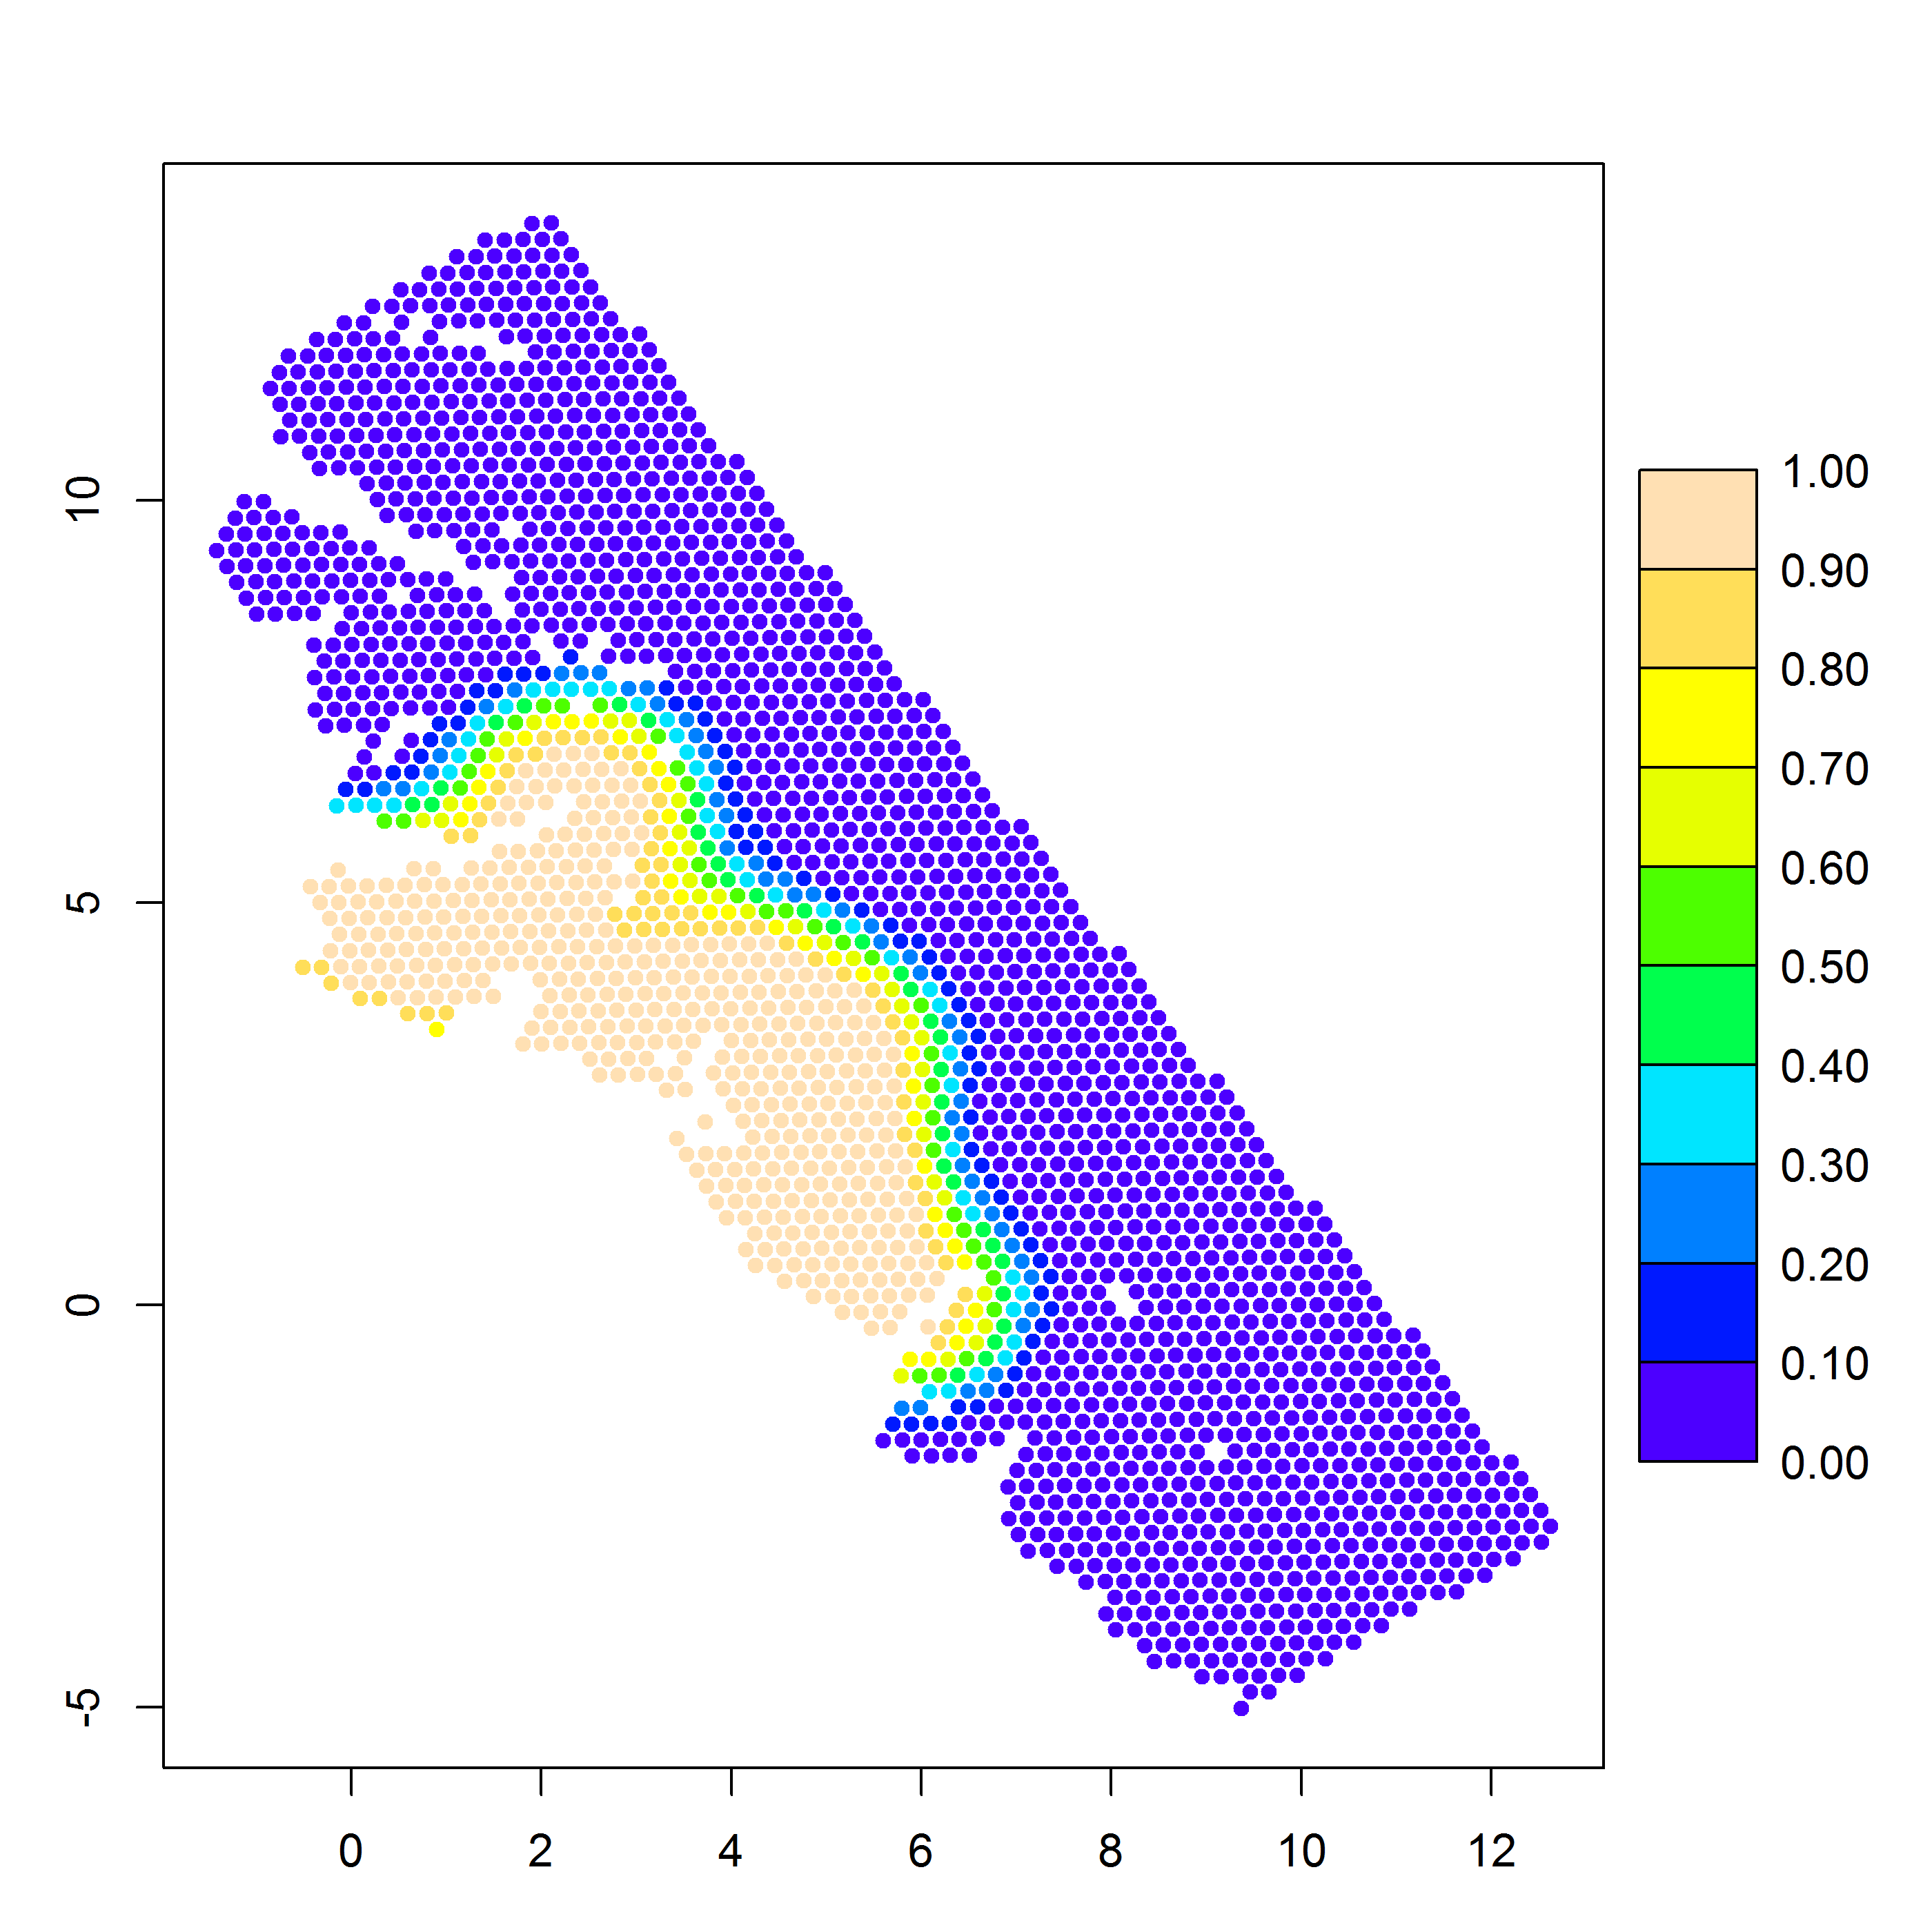
\includegraphics[height=3in]{Ch5-SCR0/figs/wolv_esa}
\end{center}
\caption{Probability of encounter used in computing effective sampled
  area for the wolverine camera trapping array, using the parameter
  estimates (posterior means) for the $2 \times 2$ km habitat mask.  }
\label{scr0.fig.esa}
\end{figure}

















\begin{comment}
\subsection{SCR models as multi-state models}

While we invoke a discrete state-space artificially, by griding the
underlying continuous state-space, sometimes the state-space is more
naturally discrete. Consider a situation in which discrete patches of
habitat are searched using some method and it might be convenient (or
occur inadvertently) to associate samples to the patch level instead
of recording observation locations. In this case we might use a model
${\bf s}_{i} \sim dcat(probs[])$  where $probs[]$ are the probabilities that
an individual inhabits a particular patch. We consider such a case
study in Chapt. XX Poisson XXX from \citet{mollet_etal:2012} who
obtained a population size estimate of a large grouse species known as
the capracaillie. Forest patches were searched for scat which was
identified to individual by DNA analysis.
Even when space is {\it not}
naturally discrete, measurements are often made at a fairly coarse
grain (e.g., meters or tens of meters along a stream), or associated
with spatial quadrats for scat searches and therefore the state-space
may be effectively discrete in many situations.

This discrete formulation of SCR models suggests that SCR models are
related to ordinary multi-state models \citep[][ch. 9]{kery_schaub:2011}
which are also parameterized in terms of a discrete state
variable which is often defined as a spatially-indexed state related
either to location of capture or breeding location. While many
multi-state models exist in which the state variable is not related to
space, multi-state models have been extremely useful in development
models of movements among geographic states and indeed this type of
problem motivated their early developments by \citet{arnason:1972,
  arnason:1973} and \citet{hestbeck_etal:1991}.  We pursue this
connection a little bit more in chapter XXX XYZ.

\end{comment}



\section{ Summary and Outlook }

In this chapter, we introduced the simplest SCR model -- ``model
SCR0'' -- which is an ordinary capture-recapture model like model
$M_0$, but augmented with a set of latent individual effects, ${\bf
  s}_{i}$, which relate encounter probability to some sense of
individual location using a covariate, ``distance'', from ${\bf
  s}_{i}$ to each trap location.  Thus, individuals in close proximity
to a trap will have a higher probability of encounter, and {\it vice
  versa}.  The explicit modeling of individual locations and distance
in this fashion resolves classical problems related to estimating
density: unknown sample area, and heterogeneous encounter probability
due to variable exposure to traps.

SCR models are closely related to 
classical individual covariate models (``model $M_{x}$'', as introduced in
Chapt. \ref{chapt.closed}), but with imperfect information about the
individual covariate. Therefore, 
they are also not too dissimilar from standard GLMMs used throughout
statistics and, as a result, we 
find that they are  easy to analyze using standard MCMC
methods encased in black boxes such as {\bf WinBUGS} or {\bf JAGS}.
We will also see that they are easy to analyze using
likelihood methods, which we address in Chapt. \ref{chapt.mle}.

Formal consideration of the collection of individual locations $({\bf
  s}_{1}, \ldots, {\bf s}_{N})$ is fundamental to all of the models
considered in this book. In statistical terminology, we think of the
collection of points $\{ {\bf s}_{i} \}$ as a realization of a point
process.  Because SCR models formally link individual encounter
history data to an underlying point process, we can obtain formal
inferences about the point process. For example, we showed how to
produce a density map (Fig. \ref{scr0.fig.density}). We can do
traditional point process analyses such as testing for ``complete
spatial randomness'' (CSR) (see Chapt.  \ref{chapt.gof}), and related
point process summaries \citep{illian_etal:2008}.

Part of the promise, and ongoing challenge, of SCR
models is to develop models that reflect interesting biological
processes, for example interactions among points or temporal dynamics
in point locations.  In this chapter  we considered the simplest possible point
process model in which points are independent and uniformly
(``randomly'') distributed over space. Despite the simplicity of this
model, it should suffice in many applications of SCR models,
although we do address generalizations in later
chapters. Moreover, even though the {\it prior} distribution on the
point locations is uniform, the realized pattern may deviate markedly
from uniformity as the observed encounter data provide information to
impart deviations from uniformity. Thus,  estimated density maps
will typically appear distinctly non-uniform (as we saw in the
wolverine example).
In
applications of the basic SCR model, we find that this simple {\it a priori}
model can effectively reflect or adapt to complex realizations of the
underlying point process.  For example, if individuals are highly
territorial then the data should indicate this in the form of
individuals not being encountered in the same trap -- the resulting
posterior distribution of point locations should therefore reflect
non-independence.  Obviously the complexity of posterior estimates of
the point pattern will depend on the quantity of data, both number of
individuals and captures per individual.  Because the point process is
such an integral component of SCR models, the state-space of the point
process plays an important role in developing SCR models. As we
emphasized in this chapter, the state-space is part of
the model. It can have an influence on parameter estimates and other
inferences, such as model selection (see chapter \ref{chapt.gof}).


One concept we introduced in this chapter, which has not
 been discussed much in the literature on SCR models,
is the manner in which the encounter probability model relates to a
model of space usage by individuals. The standard SCR models of
encounter probability can all be motivated as simplistic models of
space usage and movement, in which individuals make random use
decisions from a probability distribution proportional to the
encounter probability model. This both clarifies the simplicity of the
underlying model of space usage and also suggests a direct extension
to produce more realistic models, which we discuss in
Chapt. \ref{chapt.rsf}.
We consider some other important extensions of the basic SCR model in
later chapters.
For example, we consider models that include covariates
that vary by individual, trap, or over time (Chapt.
\ref{chapt.covariates}), spatial covariates on density (Chapt.
\ref{chapt.state-space}), open populations (Chapt. \ref{chapt.open}),
and methods for model assessment and selection
(Chapt. \ref{chapt.gof}) among other topics.  We also consider
technical details of
 maximum likelihood (Chapt.  \ref{chapt.mle}) and
Bayesian (Chapt.  \ref{chapt.mcmc}) estimation,
so that the interested
reader can develop or extend methods to suit their own needs.


\begin{comment}
xxxxx$I would tone down the next paragraph. Also, after having read this chapter (and understood at least the main things in it), this question does not strike me as very obvious anymore$ xxxxxAn obvious question that might be floating around in your mind is why
should we ever go through all of this trouble when we could just use
{\bf MARK} or {\bf CAPTURE} xxx$this bold face is intrusive on the eye$ xxxxxto get an estimate of $N$ and apply $1/2$
MMDM methods?  The main reason is that these conventional methods are
predicated on models that represent explicit misspecifications of both
the observation and ecological process - they are wrong!  Not just
wrong, because of course all models are wrong, but they're not even
{\it plausible} models! Thus while we might be able to show adequate
fit or whatever, we think as a conceptual and philosophical model one
should not be using models that are not even plausible data-generating
models -- even if the plausible ones don't fit!  Perhaps more
charitably, these ordinary non-spatial models are models of the wrong
system. They do not account for trap identity. They don't account for
spatial organization or clustering of individual encounters in
space. And, density is not estimable from such models because
it has no meaning absent an explicit representation of space. If
we do define space explicitly, e.g., as a buffered minimum convex
hull, then the normal models ($M_{0}$, $M_{h}$, etc..) assume that
individual capture-probability is not related to space, no matter how
we define the buffer.  Conversely, the SCR model is a model for
trap-specific encounter data - how individuals are organized in space
and interact with traps. SCR models provide a coherent framework for
inference about density or population size and also, because of the
formality of their derivation, can be extended and generalized to a
large variety of different situations, as we demonstrate in subsequent
chapters.
\end{comment}


\chapter{
Likelihood Analysis of Spatial Capture-Recapture Models
}
\markboth{Likelihood Estimation}{}
\label{chapt.mle}

\vspace{.3in}

We have so far mainly focused on Bayesian analysis of spatial
capture-recapture models. And, in the previous chapters we learned how
to fit some basic spatial capture-recapture models using a Bayesian
formulation of the models analyzed in {\bf BUGS} engines including {\bf
  WinBUGS} and {\bf JAGS}.  Despite our focus on Bayesian analysis, it
is instructive to develop the basic concepts and ideas behind
classical analysis based on likelihood methods and frequentist
inference for SCR models. This has been the approach taken by
\citet{borchers_efford:2008, dawson_efford:2009} and related papers.
Therefore, in this chapter, we provide some conceptual and technical
foundation for likelihood-based analysis of spatial capture-recapture
models. We recognized earlier (Chapt. \ref{chapt.scr0}) that SCR
models are versions of binomial (or other) GLMs, but with random
effects (i.e., GLMMs). 
Throughout statistics, such models 
are routinely analyzed by
likelihood methods. In particular, likelihood analysis is based on the
integrated or marginal likelihood in which the random effects are removed, by
integration, from the conditional-on-${\bf s}$ likelihood. 


We will show here that it is straightforward to compute the maximum
likelihood estimates (MLE) for SCR models by integrated 
likelihood. We develop the MLE framework using {\bf R}, and we also
provide a basic introduction to an {\bf R} package \mbox{\tt secr}
\citep{efford:2011} which mostly does likelihood analysis of SCR
models (see also the the stand-alone package {\bf DENSITY}
\citep{efford_etal:2004}).  To set the context for likelihood analysis
of SCR models, we first analyze the SCR model here when $N$ is known
because, in that case, analysis is no different at all than a standard
GLMM.
We generalize the model to allow for unknown $N$
using both conventional ideas based on the ``joint likelihood''
\citep[e.g.,][]{borchers_etal:2002} and also using a formulation based
on data augmentation.  We obtain the MLEs for the SCR model from the
wolverine camera trapping study \citep{magoun_etal:2011} analyzed in
previous chapters to compare/contrast the results.

\section{MLE with known N}

We noted in Chapt. \ref{chapt.scr0} that, with $N$ known, the basic SCR model is a
type of binomial regression with a random effect. For such models we
can  obtain maximum likelihood estimators of model parameters
based on integrated likelihood. The integrated likelihood is based on
the marginal distribution of the data $y$ in which the random effects
are removed by integration from the conditional-on-${\bf s}$ distribution of the
observations. See Chapt. \ref{chapt.modeling} for a
review of marginal, conditional and joint distributions.
Conceptually, any SCR model begins with a specification
of the conditional-on-${\bf s}$ model $[y|{\bf s},{\bm \alpha}]$ and we have
a ``prior distribution'' for ${\bf s}$, say $[{\bf s}]$. Then, the
marginal distribution of the data $y$ is
\[
[y|{\bm \alpha}] =  \int_{\bf s} [y|{\bf s},{\bm \alpha}][{\bf s}] d{\bf s}.
\]
When viewed as a function of ${\bm \alpha}$ for purposes of estimation, the
marginal distribution $[y|{\bm \alpha}]$ is often referred to as the {\it
  integrated likelihood}.

It is worth analyzing 
the simplest SCR model with known-$N$ in order to understand the
underlying mechanics and basic concepts. These are directly relevant to
the manner in which many capture-recapture models are classically
analyzed, such as model $M_h$, and individual covariate models (see
Chapt. \ref{chapt.closed}).

 To develop the integrated
likelihood for SCR models, we first identify the conditional-on-${\bf s}$
likelihood. 
The observation model for each encounter observation $y_{ij}$, for
individual $i$ and trap $j$,
specified conditional on ${\bf s}_{i}$, is 
\begin{equation}
y_{ij}| {\bf s}_{i} \sim \mbox{Binomial}(K, p_{\alpha}({\bf x}_{j},{\bf s}_{i}))
\label{mle.eq.cond-on-s}
\end{equation}
where we have indicated the dependence of $p_{ij}$ on ${\bf s}$ and
parameters ${\bm \alpha}$
explicitly. For example, $p_{ij}$ might be the Gaussian model given by
\[
 p_{ij} = \mbox{logit}^{-1}(\alpha_{0})\exp( -\alpha_{1} ||{\bf x}_{j} - {\bf s}_{i}||)
\]
where $\alpha_{1} = 1/(2\sigma^2)$.
%Further, the distribution of the random effect is ${\bf s}_{i} \sim  \mbox{Uniform}({\cal
%%  S})$.
The joint distribution of the data for individual $i$ is the product
of $J$ such terms (i.e., contributions from each of $J$ traps).
\[
  [{\bf y}_{i} | {\bf s}_{i} , {\bm \alpha}] = 
  \prod_{j=1}^{J} \mbox{Binomial}(K, p_{\alpha}({\bf x}_{j},{\bf s}_{i}) )
\]
We note this assumes that encounter of individual $i$ in each
trap is independent of encounter in every other trap, conditional on
${\bf s}_{i}$, this is the fundamental property of the basic model SCR0.


The marginal likelihood is computed by removing
${\bf s}_{i}$, by integration (hence also {\it integrated} likelihood), from the conditional-on-${\bf s}$
likelihood and regarding the {\it marginal} distribution of the data
as 
the likelihood. That
is, we compute:
\[
  [{\bf y}|{\bm \alpha}] = 
\int_{{\cal S}}  [ {\bf y}_{i} |{\bf s}_{i}, {\bm \alpha}] [{\bf s}_{i}] d{\bf s}_{i}
\]
In most SCR models, $[{\bf s}] = 1/A({\cal S})$ where $A({\cal S})$ is
the area of the prescribed state-space ${\cal S}$ (but see Chapt. \ref{chapt.state-space} for
alternative specifications of $[{\bf s}]$).

The joint likelihood for all $N$ individuals, assuming independence of
encounters among individuals, is the product of $N$ such terms:
\[
{\cal L}({\bm \alpha} | {\bf y}_{1},{\bf y}_{2},\ldots, {\bf y}_{N}) =     \prod_{i=1}^{N}
[{\bf y}_{i}|{\bm \alpha}]
\]
We emphasize that two independence assumptions are explicit in this
development: independence of trap-specific encounters within
individuals and also independence among individuals. In particular,
this would only be valid when individuals are not physically
restrained or removed upon capture, and when traps do not ``fill up''
(i.e., this is model SCR0, from Chapt. \ref{chapt.scr0}).

The key operation for computing the likelihood is solving a
2-dimensional integration problem. There are some general purpose {\bf
  R} packages that implement a number of 
 multi-dimensional integration routines
including \mbox{\tt adapt} \citep{genz_etal:2007} and \mbox{\tt R2cuba}
\citep{hahn_etal:2011}.  In practice, we won't rely
on these extraneous {\bf R} packages (except see
Chapt. \ref{chapt.state-space} for an application of \mbox{\tt R2cuba})
but instead will use perhaps less
efficient methods in which we replace the integral with a summation
over an equal area mesh of points on the state-space ${\cal S}$ and explicitly
evaluate the integrand at each point. We invoke the rectangular rule
for integration here\footnote{e.g., 
\url{http://en.wikipedia.org/wiki/Rectangle_method}
} in which we
evaluate the
integrand on a regular grid of points of equal area and compute the
average of
the integrand over that grid of points. 
Let $u=1,2,\ldots,nG$ index a grid of
$nG$ points, ${\bf s}_{u}$,  where the area of grid cells is
constant, say $A$.
In this case, the integrand, i.e., the marginal pmf of 
${\bf y}_{i}$, is approximated by  
\begin{equation}
         [{\bf y}_{i}|{\bm \alpha}] = \frac{1}{nG} \sum_{u=1}^{nG}  [ {\bf
            y}_{i} |{\bf s}_u, {\bm \alpha}]
\label{mle.eq.intlik}
\end{equation}

This is a specific case of the general expression that could be used
for approximating the integral for any arbitrary 
distribution $[{\bf s}]$. The general case is
\[
[{\bf y}|{\bm \alpha}]  = \frac{A({\cal S})}{nG} \sum_{u=1}^{nG} [y|{\bf s}_{u},{\bm \alpha}] [{\bf s}_{u}]
\]
Under the uniformity assumption,
 $[{\bf s}] = 1/A({\cal S})$
and thus the grid-cell area cancels in the above
expression to yield eq. \ref{mle.eq.intlik}.
The rectangular rule for integration can be seen as an application of
the Law of Total Probability for a discrete random variable ${\bf
  s}$, having $nG$ 
unique values with equal probabilities $1/nG$.


\subsection{Implementation (simulated data)}

Here we will illustrate how to carry out this integration and
optimization based on the integrated likelihood using simulated data
 (i.e., see Sec. \ref{scr0.sec.simulating}). Using \mbox{\tt simSCR0}
 we simulate data for 100 individuals and an array of 25 traps
laid out in a $5 \times 5$ grid of traps having unit spacing.  The specific encounter
model is the Gaussian model. The 100 activity centers were
simulated on a state-space defined by an $8 \times 8$ square 
within which the
trap array was centered (thus the trap array is buffered by 2
units). Therefore, the density of individuals in this system is fixed
at $100/64$.
In the following set of {\bf R} commands we generate the data and 
then harvest the required data objects:
{\small
\begin{verbatim}
  ## simulate a complete data set (perfect detection)
> data <- simSCR0(discard0=FALSE,rnd=2013)
  ## extract the objects that we need for analysis
> y <- data$Y
> traplocs <- data$traplocs
> nind <- nrow(y)  ## in this case nind=N
> J <- nrow(traplocs)
> K <- data$K
> xlim <- data$xlim
> ylim <- data$ylim
\end{verbatim}
}
{\flushleft Now } we need to define the integration grid, say
\mbox{\tt G}, which we do with
the following set of {\bf R} commands (here, \mbox{\tt delta} is the grid spacing):
{\small
\begin{verbatim}
> delta <- .2
> xg <- seq(xlim[1]+delta/2,xlim[2]-delta/2,by=delta) 
> yg <- seq(ylim[1]+delta/2,ylim[2]-delta/2,by=delta) 
> npix <- length(xg)          # valid for square state-space only
> G <- cbind(rep(xg,npix),sort(rep(yg,npix)))
> nG <- nrow(G)
\end{verbatim}
}
{\flushleft In this case}, the integration grid is set up as a grid with spacing
$\delta = 0.2$ which produces, for our example, a $40 \times 40$ grid of points for evaluating the
integrand if the state-space buffer is set at 2. We note that the
integration grid is set-up here to correspond exactly to the
state-space used in simulating the data. However, in practice, we
wouldn't know this, and our estimate of $N$ (for the unknown case, see
below) would be sensitive to choice of the extent of the integration
grid. As we've discussed previously, density, which is $N$
standardized by the area of the state-space, will not be so sensitive
in most cases. 

We are now ready to  compute the conditional-on-{\bf s} likelihood and
carry out the marginalization described by Eq. \ref{mle.eq.intlik}.
We need to do this by defining an {\bf R} function that computes the
likelihood for the integration grid, as a function of the data objects \mbox{\tt y} and
\mbox{\tt traplocs} which were created above. However,
it is a bit untidy to store the grid information in your workspace,
and define the likelihood function in a way that depends on these things that
exist in your workspace.  Therefore, we build the {\bf R} function so
that it computes the integration grid {\it within} the function, thereby
avoiding potential problems if our trapping grid locations change, or
if we want to modify the state-space buffer easily.  We therefore
define the function, called \mbox{\tt intlik1}, to which we pass the data
objects and other information necessary to compute the marginal
likelihood.  This function is available in the \mbox{\tt scrbook}
package (use {\tt ?intlik1} at the {\bf R} prompt).  The code is
reproduced here:

{\small 
\begin{verbatim}
intlik1 <- function(parm,y=y,delta=.2,X=traplocs,ssbuffer=2){

Xl<-min(X[,1]) - ssbuffer   ## these lines of code are setting up the 
Xu<-max(X[,1]) + ssbuffer   ## support for the integration which is
Yu<-max(X[,2]) + ssbuffer   ## the same as the state-space of "s"
Yl<-min(X[,2]) - ssbuffer
xg<-seq(Xl+delta/2,Xu-delta/2,,length=npix) 
yg<-seq(Yl+delta/2,Yu-delta/2,,length=npix) 
npix<-length(xg)

G<-cbind(rep(xg,npix),sort(rep(yg,npix)))
nG<-nrow(G)
D<- e2dist(X,G)  

alpha0<-parm[1]
alpha1<-exp(parm[2])  # alpha1 restricted to be positive here
                      # for convenience (it is negated below)
probcap<- plogis(alpha0)*exp(-alpha1*D*D)
Pm<-matrix(NA,nrow=nrow(probcap),ncol=ncol(probcap))
                    # all zero encounter histories
n0<-sum(apply(y,1,sum)==0) 
                    # encounter histories with at least 1 detection
ymat<-y[apply(y,1,sum)>0,] 
ymat<-rbind(ymat,rep(0,ncol(ymat)))
lik.marg<-rep(NA,nrow(ymat))
for(i in 1:nrow(ymat)){
 ## next line: log conditional likelihood for ALL possible values of s
Pm[1:length(Pm)]<- 
      (dbinom(rep(ymat[i,],nG),K,probcap[1:length(Pm)],log=TRUE))
 ## next line: sum the log conditional likelihoods, exp() result
 ## same as taking the product
lik.cond<- exp(colSums(Pm))
 ## take the average value == computing marginal
lik.marg[i]<- sum( lik.cond*(1/nG))  
}
 ## n0 = number of all-0 encounter histories
nv<-c(rep(1,length(lik.marg)-1),n0)
-1*( sum(nv*log(lik.marg)) )
}
\end{verbatim}
}


The function \mbox{\tt intlik1} accepts as input the encounter history
matrix, \mbox{\tt y}, the
trap locations, \mbox{\tt X}, and the state-space buffer. This allows us to
vary the state-space buffer and easily evaluate the sensitivity of the
MLE to the size of the state-space.  Note that we have a peculiar
handling of the encounter history matrix \mbox{\tt y}. In particular, we remove
the all-zero encounter histories from the matrix and tack-on a single
all-zero encounter history as the last row which then gets weighted by
the number of such encounter histories (\mbox{\tt n0}). This is a bit
long-winded and strictly unnecessary when $N$ is known, but we did it
this way because the extension to the unknown-$N$ case is now
transparent (as we demonstrate in the following section).  The matrix
\mbox{\tt Pm} holds the log-likelihood contributions of each encounter
frequency for each possible state-space location of the individual.
The log contributions are summed up and the result exponentiated on
the next line, producing lik.cond, the conditional-on-${\bf s}$
likelihood (Eq. \ref{mle.eq.cond-on-s} above). The marginal likelihood
(\mbox{\tt lik.marg}) sums up the conditional elements weighted by the probabilities
$[{\bf s}]$ (Eq. \ref{mle.eq.intlik} above).  This is a fairly
primitive function which doesn't allow much flexibility in the data
structure. For example, it assumes that $K$, the number of replicates,
is constant for each trap. Further, it assumes that the state-space is
a square. We generalize this to some extent later in this chapter.

Here is the {\bf R} command for maximizing the likelihood using
\mbox{\tt nlm} (the function \mbox{\tt optim} could also be used) and saving the
results into an object called \mbox{\tt frog}.  The output is a list of the
following structure and these specific estimates are produced using
the simulated data set:

{\small 
\begin{verbatim}
# should take 15-30 seconds

> starts <- c(-2,2)
> frog <- nlm(intlik1,starts,y=y,delta=.1,X=traplocs,ssbuffer=2,hessian=TRUE)
> frog

$minimum
[1] 297.1896

$estimate
[1] -2.504824  2.373343

$gradient
[1] -2.069654e-05  1.968754e-05

$hessian
          [,1]      [,2]
[1,]  48.67898 -19.25750
[2,] -19.25750  13.34114

$code
[1] 1

$iterations
[1] 11
\end{verbatim}
} 
Details about this output can be found on the help page for
\mbox{\tt nlm}. We note briefly that \mbox{\tt frog\$minimum} is the
negative log-likelihood value at the MLEs, which are stored in the
\mbox{\tt frog\$estimate} component of the list. The Hessian is the
observed Fisher information matrix, which can be inverted to obtain
the variance-covariance matrix using the command:
\begin{verbatim}
> solve(frog$hessian)
\end{verbatim}

It is worth drawing attention to the fact that the estimates are slightly
different than the Bayesian estimates reported previously in
Sec. \ref{scr0.sec.winbugs1}.   There are several reasons
for this.  First Bayesian inference is based on the posterior
distribution and it is not generally the case that the MLE should
correspond to any particular value of the posterior distribution. If
the prior distributions in a Bayesian analysis are uniform, then the
(multivariate) mode of the posterior is the MLE, but note that
Bayesians almost always report posterior {\it means} and so there will
typically be a discrepancy there. Secondly, we have implemented an
approximation to the integral here and there might be a slight bit of
error induced by that. We will evaluate that shortly. Third, the
Bayesian analysis by MCMC is itself subject to some amount of Monte Carlo
error which the analyst should always be aware of in practical
situations.  All of these different explanations are likely
responsible for some of the discrepancy. Accounting for these, we see
general consistency between the two estimates.

\begin{comment} 
To compute the integrated likelihood we used a discrete representation
of the state-space so that the integral could be approximated as a
summation over possible values of ${\bf s}$ with each value being
weighted by its probability of occurring, which is $1/nG$ under the
assumption that ${\bf s}$ is uniform on the state-space ${\cal
  S}$. Recall
in Chapt. \ref{chapt.scr0} we 
used a discrete state-space in developing a Bayesian analysis of the
model in order to be able to modify the state-space in a flexible
manner. In that case, we could use the discretized state-space as the
integration grid and just feed it into our integrated likelihood
routine. 
\end{comment}

In summary, for the basic SCR model, integrated
likelihood is a really easy calculation when $N$ is known. Even for $N$
unknown it is not too difficult, and we will do that shortly.
However, if you can solve the known-$N$ problem then you should be able
to do a real analysis, for example by considering different values of
$N$ and computing the results for each value and then making a plot of
the log-likelihood or AIC and choosing the value of $N$ that produces
the best log-likelihood or AIC. As a homework problem we suggest that
the reader take the code given above and try to estimate $N$ without
modifying the code by just repeatedly applying it for 
different values of $N$ in attempt to deduce the best value.
We will formalize the unknown-$N$ problem next.

%The
%software package {\bf DENSITY} \citep{efford_etal:2004} implements
%certain types of SCR models using integrated likelihood methods, and
%\mbox{\tt secr} \citep{efford:2011} is an {\bf R} package with similar functionality.
%We provide an analysis of some data using \mbox{\tt secr} shortly along
%with a discussion of its capabilities, and we use \mbox{\tt secr} in
%later chapters for likelihood analysis of other SCR models.


\section{MLE when N is Unknown} 
\label{mle.sec.Nunknown}

Here we build on the previous introduction to integrated likelihood
but we consider now the case in which $N$ is unknown. We will see that
adapting the analysis based on the known-$N$ model is 
straightforward for the more general problem. The main distinction is
that we don't observe the all-zero encounter history so we have to
make sure we compute the probability for that encounter history which
we do by tacking a row of zeros onto the encounter history matrix. In
addition, we include the number of such all-zero encounter histories
(that is, the number of individuals {\it not} encountered)
as an unknown parameter of the model. Call that unknown quantity
$n_{0}$. Then, $N=n_{0}+n$. We will usually parameterize the
likelihood in terms of $n_{0}$ because optimization over a parameter
space in which $\log(n_{0})$ is unconstrained is preferred to a
parameter space in which $N$ must be constrained $N\ge n$.
With $n_{0}$ unknown, we have to be sure to include a combinatorial term to
account for the fact that of the $n$ observed individuals there are
${N \choose n}$ 
ways to realize a sample of size $n$. The
combinatorial term involves the unknown $n_{0}$ and thus it must be
included in the likelihood. In evaluating the  log-likelihood, we
have to compute terms such as the log-factorial $\log(N!) = \log((n_{0}+n)!)$. 
We do this in {\bf R} by making use of the log-gamma function
(\mbox{\tt lgamma}) and the identity
\[
 \log(N!) = \mbox{\tt lgamma}(N+1).
\]

Therefore, to compute the likelihood, we require 
the following 3 components: (1) The marginal
probability of each ${\bf y}_{i}$ as before,
\[
  [{\bf y}_{i}|{\bm \alpha}] = 
\int_{{\cal S}} [{\bf y}_{i} |{\bf s}_{i}, {\bm
  \alpha}] [{\bf s}_{i}] d{\bf s}_{i}.
\]
(2) We compute
the probability of an all-0 encounter history:
\[
\pi_{0} = [{\bf y} = {\bf 0} | {\bm \alpha}] = 
\int_{{\cal S}} \mbox{Binomial}({\bf 0} |{\bf s}_{i}, {\bm \alpha})[{\bf s}_{i}] d{\bf s}_{i}
\]
(3) The combinatorial term: ${N \choose n}$. Then, 
 the marginal likelihood has this form:
\begin{equation}
 {\cal L}({\bm \alpha}, n_{0}| {\bf y})  = \frac{N!}{n! n_{0}!}
 \left\{ \prod_{i=1}^{n}  [{\bf y}_{i}|{\bm \alpha}] \right\}
\pi_{0}^{n_{0}}.
\label{mle.eq.binomialform}
\end{equation}
This is discussed in \citet[][p. 379]{borchers_efford:2008} as the
conditional-on-$N$ form of the likelihood -- we might also call it
the ``binomial form'' because of its appearance. 

Operationally, things proceed much as before: 
We compute the marginal probability of each observed ${\bf y}_{i}$,
i.e., by removing the latent ${\bf s}_{i}$ by integration. In
addition, we 
 compute the marginal probability of the ``all-zero'' encounter
history ${\bf y}_{n+1}$, and make sure to weight it $n_{0}$ times. We
accomplish this by ``padding'' the data set with a single encounter
history having $y_{n+1,j}=0$ for all traps $j=1,2,\ldots,J$. Then we
be sure to include the combinatorial term in the likelihood or
log-likelihood computation. We demonstrate this shortly.
To analyze a specific case, we'll read in our fake data set (simulated
using the parameters given above). To set some things up in our
workspace we do this:
\begin{verbatim}
data <- simSCR0(discard0=TRUE,rnd=2013)  # obtain a simulated data set
  ## extract the items we need for analysis
y <- data$Y
nind <- nrow(y)
traplocs <- data$traplocs
J <- nrow(traplocs)
K <- data$K
\end{verbatim}
Recall that these data were generated with $N=100$, on an $8 \times 8$ unit
state-space representing the trap locations  buffered by 2 units.

As before, the likelihood is defined in the {\bf R} workspace as an
{\bf R}
function, \mbox{\tt intlik2}, 
 which takes an argument being the unknown parameters of the
model and additional arguments as prescribed. In particular, 
 we provide the encounter history matrix ${\bf y}$, the trap locations
\mbox{\tt traplocs}, the spacing of the integration grid (argument
\mbox{\tt delta}) and the
state-space buffer. Here is the new likelihood function: 
{\small
\begin{verbatim}
intlik2 <- function(parm,y=y,delta=.3,X=traplocs,ssbuffer=2){

Xl<-min(X[,1]) - ssbuffer
Xu<-max(X[,1]) + ssbuffer
Yu<-max(X[,2]) + ssbuffer
Yl<-min(X[,2]) - ssbuffer

xg<-seq(Xl+delta/2,Xu-delta/2,delta) 
yg<-seq(Yl+delta/2,Yu-delta/2,delta) 
npix.x<-length(xg)
npix.y<-length(yg)
area<- (Xu-Xl)*(Yu-Yl)/((npix.x)*(npix.y))
G<-cbind(rep(xg,npix.y),sort(rep(yg,npix.x)))
nG<-nrow(G)
D<- e2dist(X,G) 
    # extract the parameters from the input vector
alpha0<-parm[1]
alpha1<-exp(parm[2])
n0<-exp(parm[3])  # note parm[3] lives on the real line
probcap<- plogis(alpha0)*exp(-alpha1*D*D)
Pm<-matrix(NA,nrow=nrow(probcap),ncol=ncol(probcap))
ymat<-rbind(y,rep(0,ncol(y)))

lik.marg<-rep(NA,nrow(ymat))
for(i in 1:nrow(ymat)){
Pm[1:length(Pm)]<- (dbinom(rep(ymat[i,],nG),K,probcap[1:length(Pm)],log=TRUE))
lik.cond<- exp(colSums(Pm))
lik.marg[i]<- sum( lik.cond*(1/nG) )  
}                                                 
nv<-c(rep(1,length(lik.marg)-1),n0)
 ## part1 here is the combinatorial term. 
 ## math: log(factorial(N)) = lgamma(N+1)
part1<- lgamma(nrow(y)+n0+1) - lgamma(n0+1)
part2<- sum(nv*log(lik.marg))
 -1*(part1+ part2)
}
\end{verbatim}
} 
To execute this function for the data that we created with \mbox{\tt
  simSCR0}, we execute the following command (saving the result in our
friend \mbox{\tt frog}).  This results in the usual output, including
the parameter estimates, the gradient, and the numerical Hessian which
is useful for obtaining asymptotic standard errors (see below):
\begin{verbatim}
> starts <- c(-2.5,0,4)
> frog <- nlm(intlik2,starts,hessian=TRUE,y=y,X=traplocs,delta=.2,ssbuffer=2)

Warning message:
In nlm(intlik2, starts, hessian = TRUE, y = y, X = traplocs, delta = 0.2,  :
  NA/Inf replaced by maximum positive value

> frog
$minimum
[1] 113.5004

$estimate
[1] -2.538333  0.902807  4.232810

[... additional output deleted ...]
\end{verbatim}
Executing \mbox{\tt nlm} here
 usually produces one or more {\bf R} warnings due to numerical
calculations happening on extremely small or large numbers
(calculation of $p$ near the
edge of the state-space), and they also happen if a poor
parameterization is used which produces evaluations of the objective
function beyond the boundary of the parameter space (e.g., $n_{0} <
0$). Such numerical warnings can often be minimized or avoided
altogether by picking judicious starting values of parameters or
properly transforming or scaling the parameters.
You will see from the \mbox{\tt nlm} output that can be reproduced that the
algorithm performed satisfactory in minimizing the objective function.
The estimate of population size for the state-space (using the default 
state-space buffer) is
\begin{verbatim}
nrow(y)+exp(4.2328)
[1] 110.9099
\end{verbatim}
Which differs from the data-generating value ($N=100$) as we might
expect for a single realization. We usually will present an estimate of uncertainty associated
with this MLE which we can obtain by inverting the Hessian. Note that
$\mbox{Var}(\hat{N}) = n + \mbox{Var}(\hat{n}_{0})$.
Since we
have parameterized the model in terms of log($n_{0}$) we use the delta
method\footnote{
We found a good set of notes on the delta approximation on Dr. David
Patterson's ST549 notes: 
\url{http://www.math.umt.edu/patterson/549/Delta.pdf}
}
described in 
\citet[][Appendix F4]{williams_etal:2002}  \citep[see also][]{verhoef:2012}
 to obtain the variance on the scale of $n_{0}$ as
follows:
\begin{verbatim}
(exp(4.2328)^2)*solve(frog$hessian)[3,3]
[1] 260.2033
> sqrt(260)
[1] 16.12452
\end{verbatim}
Therefore, the asymptotic ``Wald-type'' confidence interval for $N$ is
$110.91 \pm 1.96 \times 16.125 = (79.305, 142.515)$. To report this in
terms of density, we scale appropriately by the area of the prescribed
state-space which is $64$ units of area (i.e., an $8 \times 8$ square).
Our MLE of $D$ is $\hat{D} = 110.91/64  = 1.733$ individuals per
square unit.



\begin{comment}

\subsection{Exercises}

{\flushleft 
{\bf 1.}	
Run the analysis with different state-space buffers and comment on the result. 
}


{\flushleft 
{\bf 2.} Conduct a brief simulation study using this code by
  simulating 100 data sets and obtain the MLEs for each data set. Do
  things seem to be working as you expect?  }

{\flushleft 
{\bf 3.} 
Further extensions: It should be straightforward to
  generalize the integrated likelihood function to accommodate many
  different situations. For examples, if we want to include more
  covariates in the model we can just add stuff to the object \mbox{\tt probcap},
 and add the relevant parameters to the argument that gets
  passed to the main  function.  For the simulated data, make up a
  covariate by generating a Bernoulli covariate (``trap type'', perhaps
  baited or not baited) randomly and try to modify the likelihood to
  accommodate that.  }

{\flushleft {\bf 4.}  We would probably be interested in devising the
  integrated likelihood for the full 3-d encounter history array so
  that we could include temporally varying covariates. This is not
  difficult but naturally will slow down the execution
  substantially. The interested reader should try to expand the
  capabilities of this basic {\bf R} function.  }
\end{comment}




\subsection{Integrated Likelihood  under data augmentation } 
\label{mle.sec.intlikDA}

The likelihood analysis developed in the previous sections
is based on the likelihood
in which $N$ (or $n_{0}$) is an explicit parameter. This is usually called
the ``full likelihood'' or sometimes ``unconditional likelihood''
\citep{borchers_etal:2002} because it is the likelihood for all
individuals in the population, not just those which have been
captured, i.e., not that which is {\it conditional on capture}.
It is also possible to 
express an alternative unconditional  likelihood using data augmentation, replacing the
parameter $N$ with $\psi$ \citep[e.g., see Sec. 7.1.6][for an example]{royle_dorazio:2008}.
We don't go into detail here, but we note that the
likelihood under data augmentation is a zero-inflated binomial
mixture -- precisely an occupancy type model \citep{royle:2006}.
Thus, while it is possible to carry out likelihood analysis of
models under data augmentation, we primarily advocate data
augmentation for Bayesian analysis.


\subsection{ Extensions}

We have only considered basic SCR models with no additional
covariates. However, in practice, we are interested in other types of
covariate effects including ``behavioral response'', 
sex-specificity of parameters, and potentially other effects. Some of
these  can be added directly to the likelihood if the covariate is fixed
and known for all individuals captured or not. An example is a
behavioral response, which amounts to having a covariate $x_{ik}=1$ if
individual $i$ was captured prior to occasion $k$ and $x_{ik}=0$
otherwise. For uncaptured individuals, $x_{ik}=0$ for all $k$.
 \citet{royle_etal:2011jwm} called this a global behavioral
response because the covariate is defined for all traps, no matter the
trap in which an individual was captured. We could also define a {\it
  local} behavioral response which occurs at the level of the trap,
i.e., $x_{ijk}=1$ if individual $i$ was captured in trap $j$ prior to
occasion $k$, etc.. 
Trap-specific covariates such as trap type or status, or
time-specific covariates such as date, are easily accommodated as
well. As an example, \citet{kery_etal:2010} develop a model for the
European wildcat \emph{Felis silvestris}  in which traps are either baited or not (a
trap-specific covariate with only 2 values), and also encounter
probability varies over time in the form of a quadratic seasonal response.
We consider models with behavioral response or fixed covariates in
Chapt. \ref{chapt.covariates}.
The integrated likelihood routines we provided above can be
modified directly for such cases, which we leave to the interested
reader to investigate. 

Sex-specificity is more difficult to deal with since sex is not known
for uncaptured individuals (and sometimes not even for all captured
individuals).  To analyze such models, we do Bayesian analysis of the
joint likelihood using  data augmentation
\citep{gardner_etal:2010jwm,russell_etal:2012}, discussed further in
Chapt. \ref{chapt.covariates}. For such covariates (i.e., that are
not fixed and known for all individuals), it is somewhat more
challenging to do MLE based on the joint likelihood as we
have developed above. Instead it is more conventional to use what is
colloquially referred to as the ``Huggins-Alho'' type model which is
one of the approaches taken in the software package \mbox{\tt secr}
\citep[][]{efford:2011} which we describe
in Sec. \ref{mle.sec.secr} below. This idea is
motivated by thinking about unequal probability sampling methods known
as Horvitz-Thompson sampling \citep[e.g.,
see][]{overton_stehman:1995}.  



\section{Classical model selection and assessment}

In most analyses, one is interested in choosing from among various
potential models, or ranking models, or something else to do with
assessing the relative merits of a set of models. A good thing about
classical analysis based on likelihood is we can apply AIC methods
\citep{burnham_anderson:2002} without difficulty. 
%There are two
%distinct contexts for model-selection that we think are relevant to
%SCR models. First is, and AIC selecting among models that represent
%distinct biological hypotheses (e.g., covariates affecting encounter
%probability or density). 
AIC is convenient for assessing the relative
merits of these different models although if there are only a few
models it is not objectionable to use hypothesis tests or confidence
intervals to determine importance of effects. 
The second model
selection context has to do with choosing among various detection
models, although, as a general rule, we don't recommend this
application of model selection.  This is because there is hardly ever
(if at all) a rational subject-matter based reason motivating specific
distance functions. As a result, we believe that doing too much model
selection will invariably lead to over-fitting and thus over-statement
of precision. This is the main reason that we haven't loaded you down
with a basket of models for detection probability so far, although we
discuss many possibilities in Chapt. \ref{chapt.covariates}.


{\bf Goodness-of-fit or model-checking} -- For many standard capture-recapture models,
it is possible to identify goodness-of-fit statistics 
based on the
multinomial likelihood,
\citep[][Chapt. 5]{cooch_white:2006},
 and evaluate model adequacy using formal
statistical tests. Similar strategies can be applied to SCR models
using expected cell-frequencies based on the marginal distribution of
the observations. Also, because computing MLEs is somewhat more
efficient in many cases compared to Bayesian analysis, it is 
sometimes feasible to use bootstrap methods. At the present time,
we don't know of any applications of goodness-of-fit testing for SCR
models based on likelihood inference, although we discuss the use of
Bayesian p-values for assessing model fit in Chapt. \ref{chapt.gof}. An
important practical problem in trying to evaluate  goodness-of-fit is
that, in realistic sample sizes, fit tests often lack the power to
detect departures from the model under consideration and so they may
not be generally useful in practice. 


%Bayesian goodness-of-fit, which we take up in more detail in
%Chapt. \ref{chapt.gof}, is almost always addressed with Bayesian
%p-values or some other posterior predictive check
%(sec. \ref{glms.sec.gof}, \citet[][sec. 2.6]{kery:2010}).
%\citet{royle_etal:2011mee} suggested checking model fit for SCR models
%by decomposing fit into two components: (1) That of the encounter
%process model, evaluated by the expected encounter frequencies
%computed {\it conditional} on ${\bf s}$; and, (2) That of the spatial
%point process model (``spatial randomness'').


\section{Likelihood analysis of the wolverine camera trapping data}
\label{mle.sec.wolverine}


Here we compute the MLEs for the wolverine data using an expanded
version of the function we developed in the previous section. To
accommodate that each trap might be operational a variable number of
nights, we provided an additional argument to the likelihood function
(allowing for a vector ${\bf K}= (K_{1},\ldots,K_{J})$), which requires also a modification to the
construction of the likelihood.  In addition,
we accommodate  the state-space is a general rectangle, and
we included a line in the code to compute the state-space area which
we apply below for computing density.  The more general function
(\mbox{\tt intlik3}) is given in the {\bf R} package \mbox{\tt scrbook}. 
%It has a general
%purpose wrapper named \mbox{\tt scr}\footnote{Not written yet} which
%has other capabilities too.
Incidentally, this function also returns the area of the state-space for a given set
of parameter values, as an attribute to the function value, which will
be used in converting $\hat{N}$ to $\hat{D}$.
To use this function to obtain the MLEs for the wolverine camera trap
study, we execute the following commands (note: these are in the help
file and will execute if you type \mbox{\tt example(intlik3)}:
{\small
\begin{verbatim}
> library(scrbook)
> data(wolverine)
 
> traps <- wolverine$wtraps
> traplocs <- traps[,2:3]/10000
> K.wolv <- apply(traps[,4:ncol(traps)],1,sum)

> y3d <- SCR23darray(wolverine$wcaps,traps)
> y2d <- apply(y3d,c(1,3),sum)

> starts <- c(-1.5,0,3)

> frog <- nlm(intlik3,starts,hessian=TRUE,y=y2d,K=K.wolv,X=traplocs,
+             delta=.2,ssbuffer=2)

> frog
$minimum
[1] 220.4313

$estimate
[1] -2.8176120  0.2269395  3.5836875

[.... output deleted ....]
\end{verbatim}
}
Of course we're interested in obtaining an estimate of population size
for the prescribed state-space, or density, and associated measures of
uncertainty which we do using the delta method
\citep[][Appendix F4]{williams_etal:2002}.
To do all of that we need to manipulate the output of
\mbox{\tt nlm} since we have our  estimate in terms of $\mbox{\tt
  log(n0)}$. We execute the following commands:
{\small 
\begin{verbatim}
> frog <- nlm(intlik3,starts,hessian=TRUE,y=y2d,K=K.wolv,X=traplocs,delta=.2,
+             ssbuffer=2)
> Nhat <- nrow(y2d)+exp(frog$estimate[3])
> area <- attr(intlik3(starts,y=y2d,K=K.wolv,X=traplocs,delta=.2,ssbuffer=2), 
+              "SSarea")
> Dhat <- Nhat/area

> Dhat
[1] 0.5494947

> SE <- (1/area)*exp(frog$estimate[3])*sqrt(solve(frog$hessian)[3,3])

> SE
[1] 0.1087073
\end{verbatim}
} 
So our estimate of density is $0.55$ individuals per ``standardized
unit'' which is 100 $km^2$, because we divided UTM coordinates by
10000.  So this is about 5.5 individuals per 1000 $km^2$,
with a SE of around 1.09
individuals.  This compares closely with $5.77$
reported in
Sec. \ref{scr0.sec.wolverine} based on Bayesian
analysis of the model.


The effect of approximating the integral by a discrete mesh of points
is that it induces some numerical error in evaluation of the integral
and, further, that error increases as the
coarseness of the mesh increases. 
To evaluate the effect (or sensitivity) of the integration grid density, 
we obtained the MLEs for a state-space buffer of 2 (standardized
units) and for integration grid with spacing $\delta = .3, .2, .1,
.05$. The MLEs for these 4 cases including the relative runtime are
given in Table \ref{mle.tab.integration}.
We see the results change only slightly as the fineness of the
integration grid increases. Conversely, the runtime on the platform of
the day for the 4 cases increases rapidly. 
These runtimes could be regarded in
relative terms,  across platforms, for gaging the decrease in
speed as the fineness of the integration grid increases.


\begin{table}[ht]
\centering
\caption{Run time and MLEs for different integration grid resolutions
  for the wolverine camera trapping data.}
\begin{tabular}{crccc}
\hline \hline
$\delta$ &   & \multicolumn{3}{c}{Estimates} \\ \hline
         &  runtime (sec)       & $\hat{\alpha}_0$ & $\hat{\alpha}_1$ &  $\widehat{\log(n_0)}$ \\ \hline
 0.30   &  9.9  &  -2.819786 & 1.258468 & 3.569731  \\
 0.20   & 32.3  &  -2.817610 & 1.254757 & 3.583690 \\
 0.10  & 115.1  &  -2.817570 & 1.255112 & 3.599040 \\
 0.05 &  407.3 &   -2.817559&  1.255281&  3.607158 \\ \hline
\end{tabular}
\label{mle.tab.integration}
\end{table}


We studied the effect of the state-space buffer on the MLEs,
using a fixed $\delta = .2$ for all analyses. The results are show in Table \ref{mle.tab.buff}. 
We used state-space buffers
of 1 to 4 units stepped by .5. As we can see in Table \ref{mle.tab.buff}, 
the estimates of $D$ stabilize rapidly and the incremental difference
is within the numerical error associated with approximating the
integral.  

\begin{table}[ht]
\centering
\caption{Results of the effect of the state-space buffer on the MLE. 
Given here are the state-space buffer (buff), area of the state-space (area), the
MLE of $N$ ($\hat{N}$) for the prescribed state-space and the corresponding MLE of
density ($\hat{D}$).}
\begin{tabular}{crcc}
\hline \hline
buff    & area & $\hat{N}$ & $\hat{D}$ \\ \hline
 1.0 & 66.98212 & 37.73338 & 0.5633352  \\
 1.5 & 84.36242 & 46.21008 & 0.5477567  \\
 2.0 &103.74272 & 57.00617 & 0.5494956  \\
 2.5 &125.12302 & 69.03616 & 0.5517463  \\
 3.0 &148.50332 & 82.17550 & 0.5533580  \\ 
 3.5 &173.88362 & 96.44018 & 0.5546249  \\
 4.0 &201.26392 &111.83524 & 0.5556646  \\  \hline
\end{tabular}
\label{mle.tab.buff}
\end{table}


\subsection{Using a habitat mask (Restricted state-space)}
\label{mle.sec.shapefile}

In Sec. \ref{scr0.sec.discrete} we used a discrete representation of
the state-space in order to have control over its extent and
shape. This makes it easy to do things like clip out non-habitat, or
create a {\it habitat mask} which defines suitable habitat.  Clearly
that formulation of the model is relevant to the calculation of the
marginal likelihood in the sense that the discrete state-space is
equivalent to the integration grid.  Thus, for example, we could
easily compute the MLE of parameters under some model with a
restricted state-space merely by creating the required state-space at
whatever grid resolution is desired, and then inputting that
state-space into the likelihood function above, instead of computing
it in the function itself. We can easily create an explicit
state-space grid for integration from arbitrary polygons or GIS
shapefiles which we demonstrate here. Our approach
is to create the integration grid (or state-space grid) outside of the
likelihood evaluation, and then determine which points of the grid lie
in the polygon defined by the shapefile using functions in the {\bf R}
packages \mbox{\tt sp} and \mbox{\tt maptools}.  For each point in the
state-space grid (object \mbox{\tt G} in the code below which is
assumed to exist), we determine whether it is inside the
polygon\footnote{We perform this check using the {\tt over}
  function. This function takes as its second argument (among others)
  an object of the class ``SpatialPolygons'' or
  ``SpatialPolygonsDataFrame'', which can hold additional information
  for each polygon, and the output value of the function differs
  slightly for these two classes: if using a ``SpatialPolygons''
  object, the function returns a vector of length equal to the number
  of points (e.g., in the example above), but if using a
  ``SpatialPolygonsDataFrame'' it returns a data frame
  (e.g., see Sec. \ref{mcmc.sec.state-space} in
  Chapt. \ref{chapt.mcmc}). If you use the {\tt over} function, make
  sure you know the class of your second argument so that when
  processing the function output you index it correctly.}, identifying
such points with a value of \mbox{\tt mask=1} and \mbox{\tt mask=0}
for points that are {\it not} in the polygon.  We load the shapefile
which originates by an application of the \mbox{\tt readShapeSpatial}
function. We have saved the result into an {\bf R} data object called
\mbox{\tt SSp} which is in the \mbox{\tt scrbook} package.  Here are
the {\bf R} commands for doing this (see the helpfile \mbox{\tt
  ?intlik4}): {\small
\begin{verbatim}
> library(maptools)
> library(sp)
> library(scrbook)

    #### If we have the .shp file in place, we would use this command:
    ####  SSp <- readShapeSpatial('Sim_Polygon.shp')
    #### data(fakeshapefile) has SSp stored as an R data file
> data(fakeshapefile)  
> Pcoord <- SpatialPoints(G)
> PinPoly <- over(Pcoord,SSp)  ### determine if each point is in polygon
> mask <- as.numeric(!is.na(PinPoly[,1]))  ## convert to binary 0/1
> G <- G[mask==1,]
\end{verbatim}
}
We created  the function \mbox{\tt intlik4} which accepts the integration
grid as an explicit argument, and this function is also available in
the package  \mbox{\tt scrbook}.

We apply this modification to the wolverine camera trapping
study. \citet{royle_etal:2011jwm} created 2, 4 and 8 km state-space
grids so as to remove ``non-habitat'' (mostly ocean, bays, and large
lakes). We previously analyzed the model using {\bf JAGS} and {\bf WinBUGS} in
Chapt. \ref{chapt.scr0}.  To set up the wolverine data and fit the
model using maximum likelihood 
we execute the following commands:
{\small 
\begin{verbatim}
> library(scrbook)
> data(wolverine)

> traps <- wolverine$wtraps
> traplocs <- traps[,2:3]/10000
> K.wolv <- apply(traps[,4:ncol(traps)],1,sum)

> y3d <- SCR23darray(wolverine$wcaps,traps)
> y2d <- apply(y3d,c(1,3),sum)
> G <- wolverine$grid2/10000

> starts <- c(-1.5,0,3)
> frog <- nlm(intlik4,starts,hessian=TRUE,y=y2d,K=K.wolv,X=traplocs,G=G)

> frog

$minimum
[1] 225.8355

$estimate
[1] -2.9955424  0.2350885  4.1104757

[... some output deleted ...]
\end{verbatim}
}

Next we convert the parameter estimates to estimates of total
population size for the prescribed state-space, and then obtain an
estimate of density (per 1000
$\text{km}^2$) using the area computed as the number of pixels in the
state-space grid \mbox{\tt G} multiplied by the area per grid cell. In
the present case (the calculation above) we used a state-space grid
with $2 \text{km} \times 2 \text{km}$ pixels.  Finally, we compute
a standard errors using the delta approximation: 
\begin{verbatim}
area <- nrow(G)*4
Nhat <- 21+exp(frog$estimate[3])
SE <-  exp(frog$estimate[3])*sqrt(solve(frog$hessian)[3,3])
D <- (Nhat/(nrow(G)*area))*1000
SE.D <- (SE/(nrow(G)*area))*1000
\end{verbatim}
We did this for each the 2 $km$, 4 $km$ and 8 $km$ state-space grids
which produced the estimates summarized in Table \ref{mle.tab.wolv}.
These estimates compare with the 8.6 (2 km grid) and 8.2 (8 km grid)
reported in 
\citet{royle_etal:2011jwm} based on a clipped state-space as described
in Sec. \ref{scr0.sec.discrete}.

\begin{table}
\centering
\caption{MLEs for the wolverine camera trapping data using 2, 4 and 8 km state-space grids.}
\begin{tabular}{cccccccc}
\hline \hline
grid &  $\alpha_0$  &  $\alpha_1$ &   $log(n_0)$  & $N$   &  SE & D(1000) &  SE \\ \hline
2  &  -3.00 & 1.27 &4.11  &81.98& 16.31 &8.31 &1.65\\
4  &  -2.99 & 1.34  &4.16 &84.88& 16.76 &8.57& 1.69\\
8   & -3.05 & 1.08 &4.06  &78.89& 15.31 &7.85& 1.52\\   \hline
\end{tabular}
\label{mle.tab.wolv}
\end{table}


\begin{comment}
\subsection{
Exercises
}

{\flushleft
1.	Compute the 95\% confidence interval for wolverine density,
somehow. Comment on the practical implication of this level of precision.
}

{\flushleft
2.	Compute the AIC of this model and modify \mbox{\tt intlik3}
 to consider alternative link functions (at least one additional) and
 compare the  AIC of the different models and the estimates. Comment. 
}
\end{comment}


\section{DENSITY and the R package \mbox{\tt secr} }
\label{mle.sec.secr}

{\bf DENSITY} is a software program developed by \citet{efford:2004}
for fitting spatial capture-recapture models based mostly on classical
maximum likelihood estimation and related inference methods.
\citet{efford:2011} has also released an {\bf R} package called
\mbox{\tt secr}, that contains much of the functionality of {\bf
  DENSITY} but also incorporates new models and features.  Here, we
briefly introduce the \mbox{\tt secr} package which we prefer to use
instead of {\bf DENSITY} because it allows us to remain in the {\bf R}
environment for data processing and summarization. We provide a brief
introduction to \mbox{\tt secr} and some of its capabilities here, and
we also use it for doing some analysis in other parts of this book.

To install
and run models in \mbox{\tt secr}, you must download the package and
load it in
{\bf R}.
\begin{verbatim}
 install.packages("secr")
 library(secr)
\end{verbatim}
\mbox{\tt secr} allows the user to simulate data and fit a suite of models with
various detection functions and covariate responses. It also contains
a number of helpful constructor functions for creating objects of the
proper class that are recognized by other \mbox{\tt secr}
functions. We provide a brief overview of the capabilities here, but
the \mbox{\tt secr} help manual can be accessed with the command:
\begin{verbatim}
 RShowDoc("secr-manual", package = "secr")
\end{verbatim}
We note that \mbox{\tt secr} has many capabilities that we will not
cover or do so only sparingly. We encourage you to read through the
manual, the extensive documentation, and the vignettes, in order
to get a better understanding of what the package is capable of. We
also cover certain capabilities of \mbox{\tt secr} in many other
chapters. 

The main model-fitting function in   \mbox{\tt secr} is called
\mbox{\tt secr.fit}, which 
makes use of the
standard {\bf R} model specification framework with tildes. 
As an example, the equivalent of the
basic model SCR0  is fitted as follows: 
{\small
\begin{verbatim}
 secr.fit(capturedata, model = list(D  ~ 1, g0 ~ 1, sigma ~ 1), buffer = 20000)
\end{verbatim}
}
{\flushleft where} \mbox{\tt capturedata} is the  object created by \mbox{\tt secr}
containing the encounter history data and the trap information, and
the model expression \verb#g0~1# indicates the intercept-only (i.e.,
constant) model.  Note that we use $p_{0}$ for the baseline encounter
probability parameter, which is $g_{0}$ here (but the meaning of
$g_{0}$ changes depending on the model). Possible predictors for detection probability
include both pre-defined variables (e.g., \mbox{\tt t} and \mbox{\tt
  b} corresponding to ``time'' and ``behavior''), and user-defined
covariates of several kinds.  For example, to include a global
behavioral response, this would be written as \verb#g0~b#.  The
discussion of this (global versus local trap-specific behavioral
response) and other covariates is developed more in
Chapt. \ref{chapt.covariates}.  We can also model covariates on
density in \mbox{\tt secr}, which we discuss in Chapt. \ref{chapt.state-space}.

Before we can fit the models, the data must first be packaged properly
for 
\mbox{\tt secr}.  
We require data files that contain two types of information:
trap layout (location and
identification information for each trap), which is equivalent to our
trap deployment file (TDF) described in sec. \ref{scr0.sec.wolverine}
and the capture data file containing 
sampling {\it session}, animal identification, trap day, and trap
location,  equivalent in information content to our encounter data file (EDF).
Sample session can be thought of as primary period identifier in a
robust design like framework -- it could represent a yearly sample or
multiple sample periods within a year, each of them producing data on
a closed population. We discuss ``multi-session'' models in more
detail below, in Sec. \ref{mle.sec.multisession} and Chapt. \ref{chapt.hscr}.


There are three important constructor functions that help package-up
your 
data for use in \mbox{\tt secr}:
\mbox{\tt read.traps},
\mbox{\tt make.capthist} and
\mbox{\tt read.mask}. 
We provide a brief description of each here, but apply them to our
wolverine camera trapping data in the next section:
\begin{itemize}
\item[(1)] 
\mbox{\tt read.traps}: This function points to an external file {\it or}
{\bf R} data object containing the trap coordinates, and other
information, and also requires specification of the type of encounter
devices (described in the next section). A typical application of this
function looks like the following, invoking the \mbox{\tt data=} option 
when there is an existing {\bf R} object
containing the trap information:
\begin{verbatim}
trapfile <- read.traps(data=traps,detector="proximity")
\end{verbatim}
\item[(2)] \mbox{\tt make.capthist}: This function takes the EDF and combines it
with trap information, and the number of sampling occasions. A typical
application looks like this:
\begin{verbatim}
capturedata <- make.capthist(enc.data,trapfile,fmt="trapID",noccasions=165)
\end{verbatim}
See \mbox{\tt ?make.capthist} for definition of distinct file
formats. Specifying  \mbox{\tt fmt = trapID}  is equivalent to our EDF format.
\item[(3)] \mbox{\tt read.mask}: If there is a habitat mask
  available 
(as described in sec. \ref{mle.sec.shapefile}), then this function
will organize it so that \mbox{\tt secr.fit} knows what to do with it.
The function accepts either an external file name (see \mbox{\tt
  ?read.mask} for details of the structure) or a $nG \times 2$ {\bf R}
object, say \mbox{\tt mask.coords},
containing the coordinates of the mask. A typical application looks
like the following:
\begin{verbatim}
grid <- read.mask(data=mask.coords)
\end{verbatim}
\end{itemize}
These constructor functions produce output that can then be used in
the fitting of models using \mbox{\tt secr.fit}.

\subsection{Encounter device types and detection models}

The \mbox{\tt secr} package requires that you specify the type of
encounter device.  Instead of describing models by their statistical
distribution (Bernoulli, Poisson, etc..), \mbox{\tt secr} uses certain
operational classifications of detector types including 'proximity',
'multi', 'single', 'polygon' and 'signal'.  For camera trapping/hair
snares we might consider `proximity' detectors or `count' detectors.
The `proximity' detector type allows, at most, one detection of each
individual at a particular detector on any occasion (i.e., it is
equivalent to the Bernoulli or binomial encounter process model, or
model SCR0).  The `count' detector designation allows repeat
encounters of each individual at a particular detector on any
occasion.  There are other detector types that one can select such as:
`polygon' detector type which allows for a trap to be a sampled
polygon \citep{royle_young:2008} which we discuss further in
Chapt. \ref{chapt.search-encounter}, and 'signal' detector which
allows for traps that have a strength indicator, e.g., acoustic arrays
\citep{dawson_efford:2009}.
%The detector types `single' and
%'multi' can be confusing as 'multi' seems like it would appropriate
%for something like a camera trap, but instead 
The detector types 'single' and 'multi' 
refer to traps that retain individuals, thus precluding the ability
for animals to be captured in other traps during the sampling
occasion.  The 'single' type indicates trap that can only catch one
animal at a time (single-catch traps), while 'multi' indicates traps that may catch more
than one animal at a time (multi-catch). These are both variations of
the multinomial encounter models described in
Chapt. \ref{chapt.poisson-mn}.

As with all SCR models, \mbox{\tt secr} fits a detection function relating
the probability of detection to the distance of a detector from an
individual activity center. \mbox{\tt secr} allows the user to specify one of a
variety of detection functions including the commonly used
half-normal (``Gaussian''), hazard rate (``Gaussian hazard''), and
(negative) exponential models.  There are 12 different
functions as of version 2.3.1 (see Table \ref{covariates.tab.detmodels} in Chapt. \ref{chapt.covariates}), but
some are only available for simulating data.
%, and one
%should be cautious when using different detection functions as the
%interpretation of the parameters, such as $\sigma$, may not be consistent
%across formulations.  
The different detection functions are defined in
the \mbox{\tt secr} manual and can be found by calling the help function for the
detection function:
\begin{verbatim}
 ?detectfn
\end{verbatim}
It is useful to note that \mbox{\tt secr} requires the buffer distance to be
defined in meters and density will be returned as number of animals
per hectare.  Thus to make comparisons between \mbox{\tt secr} and
output from other programs, 
we will often have to convert the density to the same units.

Most of the detection functions available in \mbox{\tt secr} contain
some kind of a scale parameter which is usually labeled $\sigma$.  The
units of this parameter default to meters in the \mbox{\tt secr}
output.  We caution that the meaning of this parameter depends on the
specific detection model being used, and it should not be directly compared as a
measure of home-range size across models. Instead, as we noted in
Sec. \ref{scr0.sec.implied} every encounter probability model implies
a model of space-usage and fitted encounter models should be converted
to a common currency such as ``area used.''


\subsection{Analysis using the \mbox{\tt secr} package}
\label{mle.sec.wolvsecr}

To demonstrate the use of the \mbox{\tt secr} package, we will show
how to do the same analysis on the wolverine study as shown in
sec. \ref{scr0.sec.wolverine}. To use the \mbox{\tt secr} package, the
data need to be formatted in a similar but slightly different manner
than we use in {\bf WinBUGS}.

For example, in sec. \ref{scr0.sec.wolverine} we introduced a standard
data format for the encounter data file (EDF) and trap deployment file
(TDF). The EDF shares the same format as that used by the \mbox{\tt
  secr} package with 1 row for every encounter observation and 4
columns representing trap session ('Session'), individual identity
('ID'), sample occasion ('Occasion'), and trap identity ('trapID').
For a standard closed population study that takes place during a
single season, the 'Session' column in our case is all 1s, to indicate
a single primary sampling occasion.  In addition to providing the
encounter data file (EDF), we must tell \mbox{\tt secr} information
about the traps, which is formated as a matrix with column labels
'trapID', 'x' and 'y', the last two being the coordinates of each
trap, with additional columns representing the operational state of
each trap during each occasion (1=operational, 0=not).

We demonstrate these differences now by walking through an analysis of
the wolverine camera trapping data using \mbox{\tt secr}.  To read in
the trap locations and other related information, we make use of the
constructor function \mbox{\tt read.traps} which also requires that we
specify the detector type.  The detector type is important because it
will determine the likelihood that \mbox{\tt secr} will use to fit the
model.  Here, we have selected ``proximity'' which corresponds to the
Bernoulli encounter model in which individuals are captured at most
once in each trap during each sampling occasion: 
{\small
\begin{verbatim}
library(secr)
library(scrbook)
data(wolverine)

traps <- as.matrix(wolverine$wtraps)
dimnames(traps) <- list(NULL,c("trapID","x","y",paste("day",1:165,sep="")))
traps1 <- as.data.frame(traps[,1:3])
trapfile1 <- read.traps(data=traps1,detector="proximity")
\end{verbatim}
}
Here we note that trap coordinates are extracted from the wolverine
data but we do {\it not} standardize them. This is because
\mbox{\tt secr} defaults to coordinate scaling of meters which is the
extant scaling of the wolverine trap coordinates. Note that we add a 'trapID' column to
the trap coordinates and provide appropriate column labels to the
'traps' matrix. 
An important aspect of the
wolverine study is that while the camera traps were operated over a
165 day period, each trap was operational during only a portion of
that period. We need to provide the trap operation information which
is contained in the columns to the right of the trap coordinates in
our standard trap deployment file (TDF). Unfortunately, this is less easy to do in \mbox{\tt
  secr}, which requires an external file with a single long string of
1's and 0's indicating the days in which each trap was operational (1)
or not (0). The \mbox{\tt read.traps} function will not allow for this
 information on trap operation if the data exists as an {\bf R} object
 -- instead, we can create this external file and then read it back in
with \mbox{\tt read.traps} using these commands:
\begin{verbatim}
hold <- rep(NA,nrow(traps))
for(i in 1:nrow(traps)){
hold[i] <- paste(traps[i,4:ncol(traps)],collapse="")
}
traps1 <- cbind(traps[,1:3],"usage"=hold)

write.table(traps1, "traps.txt", row.names=FALSE, col.names=FALSE)
trapfile2 <- read.traps("traps.txt",detector="proximity") 
\end{verbatim}
These operations can be accomplished using the function \mbox{\tt
  scr2secr} which is provided in the {\bf R} package \mbox{\tt scrbook}.

After reading in the trap data, we now need to create the encounter matrix
or array using the
\mbox{\tt make.capthist} command, where we provide the capture
histories in EDF format, which is the existing format of
the data input file \mbox{\tt wcaps}.
In creating the capture history, we provide also the trapfile created
previously, the format (e.g., here EDF format is \mbox{\tt fmt=
  ``trapID''}), 
and finally, we provide the number of occasions. We also set up a
habitat mask using the $2 \times 2$ $km$ grid which we used previously
in the analysis of the wolverine data and then pass the relevant
objects to \mbox{\tt secr.fit} as follows:
{\small 
\begin{verbatim}
#
# grab the encounter data file and format it:
#
wolv.dat <- wolverine$wcaps 
dimnames(wolv.dat) <- list(NULL,c("Session","ID","Occasion","trapID"))
wolv.dat <- as.data.frame(wolv.dat)
wolvcapt2 <- make.capthist(wolv.dat,trapfile2,fmt="trapID",noccasions=165)

# grab the habitat mask (2 x 2 km) and format it:
#
gr2 <- (as.matrix(wolverine$grid2))
dimnames(gr2) <- list(NULL,c("x","y"))
gr2 <- read.mask(data=gr2)
# To fit the model we use secr.fit:
#
wolv.secr2 <- secr.fit(wolvcapt2,model=list(D ~ 1, g0 ~ 1, sigma ~ 1), 
                     buffer=20000,mask=gr2)
\end{verbatim}
}
We are using the 
basic ``proximity detector'' model (SCR0), so we do not need to make any specifications in
the command line because we have specified the detector type using the
constructor function \mbox{\tt read.traps},
except to provide the buffer size (in $m$).  To
specify different models, you can change the default
\verb#D~1, g0~1, sigma~1#, which the interested reader can do with
very little difficulty. We provide all of these commands and
additional analyses in the \mbox{\tt scrbook} package with the
function called \mbox{\tt secr\_wolverine}. Printing the output object
produces the following (slightly edited):

{\small
\begin{verbatim}
wolv.secr2

secr 2.3.1, 15:52:45 29 Aug 2012

Detector type     proximity 
Detector number   37 
Average spacing   4415.693 m 
x-range           593498 652294 m 
y-range           6296796 6361803 m 
N animals       :  21  
N detections    :  115 
N occasions     :  165 
Mask area       :  987828.1 ha 

Model           :  D ~ 1 g0 ~ 1 sigma ~ 1 
Fixed (real)    :  none 
Detection fn    :  halfnormal 
Distribution    :  poisson 
N parameters    :  3 
Log likelihood  :  -602.9207 
AIC             :  1211.841 
AICc            :  1213.253 

Beta parameters (coefficients) 
           beta    SE.beta       lcl       ucl
D     -9.390124 0.22636698 -9.833795 -8.946452
g0    -2.995611 0.16891982 -3.326688 -2.664535
sigma  8.745547 0.07664648  8.595323  8.895772

Variance-covariance matrix of beta parameters 
                  D            g0        sigma
D      0.0512420110 -0.0004113326 -0.003945371
g0    -0.0004113326  0.0285339045 -0.006269477
sigma -0.0039453711 -0.0062694767  0.005874683

Fitted (real) parameters evaluated at base levels of covariates 
       link     estimate  SE.estimate          lcl          ucl
D       log 8.354513e-05 1.915674e-05 5.360894e-05 1.301982e-04
g0    logit 4.762453e-02 7.661601e-03 3.466689e-02 6.509881e-02
sigma   log 6.282651e+03 4.822512e+02 5.406315e+03 7.301037e+03
\end{verbatim}
}

The object returned by \mbox{\tt secr.fit} provides extensive default
output when printed. Much of this is basic descriptive information
about the model, the traps, or the encounter data. We focus here on
the parameter estimates.
Under the fitted (real) parameters, we find $D$, the density, given in
units of individuals/hectare (1 hectare = 10000 $m^2$).  To convert this
into individuals/1000 km$^2$, we multiply by 100000, thus our density
estimate is 8.35 individuals/1000 km$^2$.  The parameter $\sigma$ is given in units of
meters, and so this corresponds to
 $6.283$ km.  Both of these estimates are very similar to those
obtained in our likelihood analysis summarized in Table \ref{mle.tab.wolv}
which, for the $2 \times 2$ km grid, we obtained $\hat{D} = 8.31$
with a SE of $100000 \times 
1.915674e-05 = 1.9156$
and, accounting for the scale difference (1 unit = 10000 $m$ in the
previous analysis), $\hat{\sigma} = \sqrt{1/(2\hat{\alpha}_{1})}*10000
= 6.289$ km. 
The difference in the MLE between Table \ref{mle.tab.wolv} and those
produced by \mbox{\tt secr} are likely due to subtle differences in  internal
tuning of optimization algorithms, starting values or other numerical
settings. In addition, see the next section.
On the other hand, the SE is slightly larger based on \mbox{\tt secr}
which is due to a subtle difference in the interpretation of $D$ under
the \mbox{\tt secr} model (See below). 






\begin{comment}
As an
exercise, run this analysis for 30 and 40 km buffers and compare those
found in section 4.6 under {\bf WinBUGS}.  
NOTE: The function \mbox{\tt
  secr.fit} 
will return a
warning when the buffer size appears to be too small.  This is useful
particularly with the different units being used between programs and
packages.
\end{comment}

\subsection{Likelihood Analysis in the \mbox{\tt secr} Package}
\label{mle.sec.secrguts}

The \mbox{\tt secr} package does likelihood analysis of SCR models for
most classes of models as developed by
\citet{borchers_efford:2008}. Their formulation deviates slightly from
the binomial form we presented in sec.  \ref{mle.sec.Nunknown} above
(though \citet{borchers_efford:2008} mention the binomial form).
Specifically, the likelihood that \mbox{\tt secr} implements is that
based on removing $N$ from the likelihood by integrating the binomial
likelihood (Eq.  \ref{mle.eq.binomialform} above) over a Poisson prior
for $N$ -- what we will call the {\it Poisson-integrated likelihood} as
opposed to the conditional-on-$N$ ({\it binomial-form}) considered
previously.

To develop the Poisson-integrated likelihood 
we compute the marginal
probability of each ${\bf y}_{i}$ and the probability of an all-0
encounter history, $\pi_{0}$, as before, 
to arrive at the  marginal likelihood in the binomial-form:
\[
 {\cal L}({\bm \alpha},n_{0} | {\bf y})  = \frac{N!}{n! n_{0}!} 
 \left\{ \prod_{i}  [{\bf y}_{i}|{\bm \alpha}] 
\right\}
 \pi_{0}^{n_{0}}
\]
Now, what \citet{borchers_efford:2008} do is
assume that $N \sim \mbox{Poisson}(\Lambda)$ and they do a further level
of marginalization over this prior distribution:
\[
\sum_{n_{0}=0}^{\infty}  
\frac{N!}{n! n_{0}!} 
 \left\{ \prod_{i}  [{\bf y}_{i}|{\bm \alpha}] \right\}
 \pi_{0}^{n_{0}}
\frac{\exp(-\Lambda) \Lambda^{N}}{N!}
\]
In Chapt. \ref{chapt.state-space} we write $\Lambda = \mu ||{\cal
  S}||$ where $||{\cal S}||$ is the area of the state-space, and $\mu$
is the density (``intensity'') of the point process. 
Carrying out the summation above produces exactly this marginal likelihood:
\[
{\cal L}_{2}({\bm \alpha}, \Lambda | {\bf y}) = 
 \left\{ \prod_{i}  [{\bf y}_{i}|{\bm \alpha}] \right\}  \Lambda^{n}   \exp( - \Lambda (1-\pi_{0}) )
\]
which is Eq. 2 of \citet{borchers_efford:2008} except for notational
differences. It also resembles the binomial-form of the likelihood in
Eq. \ref{mle.eq.binomialform} except with 
$\Lambda^{n}   \exp( - \Lambda \pi_{0} )$ replacing the combinatorial
term and the $\pi_{0}^{n_{0}}$ term. 
We emphasize there are two marginalizations
 going on here: (1) the
integration to remove the latent variables ${\bf s}$; and, (2) 
summation to remove the parameter $N$. 
We provide a function for
computing this in the \mbox{\tt scrbook} package called \mbox{\tt
  intlik3Poisson}. The help file for that function shows how to
conduct a small simulation study to compare the MLE under the
Poisson-integrated likelihood with that from the binomial form. 

The essential distinction between our MLE and Borchers and Efford
as implemented in \mbox{\tt secr}
is whether you keep $N$ in the model or remove it by
integration over a Poisson prior. If you have prescribed a state-space
explicitly with a sufficiently larger buffer, then we imagine there
should be hardly any difference at all between the MLEs obtained by
either the Poisson-integrated likelihood or the binomial-form of the
likelihood which retains $N$.
There is a subtle distinction in the sense that under the binomial
form, we estimate the realized population size $N$ for the state-space
whereas, for the Poisson-integrated form we estimate the {\it prior} 
expected value which would apply to a hypothetical new study of a
similar population.


Both models (likelihoods) assume ${\bf s}$ is uniformly distributed
over space, but for the binomial model we make no additional
assumption about $N$ whereas we assume $N$ is Poisson using the
formulation in \mbox{\tt secr} from \citep{borchers_efford:2008}.
Using data augmentation we could do a similar kind of integration but
integrate $N$ over a binomial ($M,\psi$) prior -- which we referred to
as the binomial-integrated likelihood in
sec. \ref{closed.sec.remarks}. So obviously the two approaches (data
augmentation and Poisson-integrated likelihood) are approximately the
same as $M$ gets large. However, doing a Bayesian analysis by MCMC, we
obtain an estimate of both $N$, the {\it realized population size},
and the parameter controlling its expected value $\psi$ which are, in
fact, both identifiable from the data even using likelihood analysis
\citep{royle_etal:2007}.  That said we can integrate $N$ out
completely and just estimate $\psi$ as we noted in sec.
\ref{mle.sec.intlikDA} above.  And we could make a prediction for a
new study which would be based on the posterior distribution of $M
\psi$ which, we imagine, should have slightly larger uncertainty
associated with it.










\subsection{Multi-Session Models in \mbox{\tt secr}}
\label{mle.sec.multisession}

In practice we will often deal with SCR data that have some meaningful
stratification or group structure.  For example, we might conduct
mist-netting of birds on $K$ consecutive days, repeated, say, $T$
times during a year, or perhaps over $T$ years. Or we might collect
data from $R$ distinct trapping grids.  In these cases, we have $T$ or
$R$ groups which we might reasonably regard as being samples of
indepdent populations.  While the groups might be distinct sites,
year, or periods within years, they could also be other biological
groups such as sex or age.  Conveniently, \mbox{\tt secr} fits a
specific model for stratified populations -- referred to as {\it
  multi-session} models. These models build on the Poisson assumption
which underlies the integrated likelihood used in \mbox{\tt secr} (as
described in the previous section).  To understand the technical
framework, let $N_{g}$ be the population size of group $g$ and {\it
  assume}
\[
 N_{g} \sim \mbox{Poisson}(\Lambda_{g}).
\]
Naturally, we model group-specific covariates on $\Lambda_{g}$:
\[
 \log(\Lambda_{g}) = \beta_{0} + \beta_{1} z_{g}
\]
where $z_{g}$ is some group-specific covariate such as a categorical index to the group, or a trend variable, or a spatial 
covariate, such as treatment effect or habitat structure, if the groups
represent spatial units. 
Under this model,  we can marginalize {\it all} $N_{g}$ parameters out
of the likelihood to concentrate the likelihood on the parameters
$\beta_{0}$ and $\beta_{1}$ precisely as discussed in the previous
section. This Poisson hierarchical model 
is the basis of the multi-session models in \mbox{\tt secr}.

To implement a multi-session model (or stratified population model) in
\mbox{\tt secr},
we provide the relevant stratification information in the 
 'Session' variable of the input encounter data file (EDF). If
 'Session' has multiple values then a
``multi-session'' object is created by default and session-specific variables can
be described in the model. For example, if the session has 2 values
for males and females then we have sex-specific densities , and
baseline encounter probability $p_{0}$ (named $g_{0}$  in \mbox{\tt
  secr}) by just doing this (see Chapt. \ref{chapt.gof} for the {\bf
  R} code to set this up):
\begin{verbatim}
> out <- secr.fit(capdata, model=list(D ~ session, g0 ~ session, sigma~ 1),
+                buffer=20000)
\end{verbatim}
More detailed analysis is given in Sec. \ref{gof.sec.aic} where we fit
a number of different models and apply methods of model selection to
obtain model-averaged estimates of density.

We can also easily implement stratified population models in the
various {\bf BUGS} engines using data augmentation
\citep{converse_royle:2012,royle_converse:2013} which we discuss, with
examples,  in Chapt. \ref{chapt.hscr}.


\subsection{Some additional capabilities of \mbox{\tt secr}}

The \mbox{\tt secr} package has capabilities to do complete analysis
of SCR data sets, including model fitting, selection, and many summary
analyses. In the previous sections, we've given a basic overview, and
we do more in later chapters of this book.  Here we mention a few of
these other capabilities that you should know about as you use
\mbox{\tt secr}. Of course, you should skim through the
associated documentation (\mbox{\tt ?secr}) to see more of whats available.

\subsubsection{Alternative observation models}
\mbox{\tt secr} fits a wide range of alternative observation models
besides the Bernoulli encounter model, including multinomial encounter
models for ``multi-catch'' and ``single catch'' traps, models for
sound attenuation from acoustic detection devices, and many others. We
discuss many of these other methods in in
Chapt. \ref{chapt.poisson-mn} and elsewhere in the book.

\subsubsection{Summary Statistics} 
\mbox{\tt secr} provides a useful default summary of the data, but it
also has summary statistics about animal movement including
mean-maximum distance moved (the function \mbox{\tt MMDM}). For example, see the help page \mbox{\tt
  ?MMDM} which lists a number of other summary functions which take a
\mbox{\tt capthist} object:
\begin{verbatim}
moves(capthist)
dbar(capthist)
RPSV(capthist)
MMDM(capthist, min.recapt = 1, full = FALSE)
ARL(capthist, min.recapt = 1, plt = FALSE, full = FALSE)
\end{verbatim}
The function \mbox{\tt moves} returns the observed distances moved,
\mbox{\tt dbar} returns the average distance moved, 
\mbox{\tt RPSV} produces a measure of dispersion about the home-range
center, 
and \mbox{\tt ARL} gives the {\it 
Asymptotic Range Length} which is the asymptote of an exponential
model fit to a scatter plot of observed range length vs. the number of
detections of each individual 
\citep{jett_nichols:1987}.




\subsubsection{State-space buffer}
\mbox{\tt secr} 
will produce a warning if the state-space buffer is chosen too
small. For example, in fitting the wolverine data as in
Sec. \ref{mle.sec.wolvsecr} but with a 1000 m buffer, 
and we see the following warning message:
{\small
\begin{verbatim}
Warning message:
In secr.fit(wolvcapt2, model=list(D ~ 1, g0 ~ 1, sigma ~ 1), buffer=1000):
  predicted relative bias exceeds 0.01 with buffer = 1000
\end{verbatim}
}
This should cause you to contemplate modifying the state-space buffer
if that is a reasonable thing to do in the specific application.


\subsubsection{Model selection and averaging}
\mbox{\tt secr} does likelihood ratio tests to compare nested models
using the function \mbox{\tt LR.test}.  You can create model selection
tables based on AIC or AICc, and obtain model-averaged parameter
estimates using \mbox{\tt model.average} (See Chapt. \ref{chapt.gof}
for examples).


\subsubsection{Population closure test}
\mbox{\tt secr} has a population closure test with the function
\mbox{\tt closure.test} which implements the tests of
\citet{stanley_burnham:1999} or \citet{otis_etal:1978}. The function
is used like this: \newline
\mbox{\tt closure.test(object, SB = FALSE)}.
Here \mbox{\tt object} is a 
capthist object and \mbox{\tt SB} is a logical variable that, if
\mbox{\tt TRUE},
produces the 
\citet{stanley_burnham:1999} test. 


\subsubsection{Density mapping and effective sample area}
\mbox{\tt secr} produces likelihood versions of the various summaries
of posterior density and effective sample area that we discussed in
Chapt. \ref{chapt.scr0}. For example, while
\mbox{\tt secr} reports estimates of density directly in the summary
output from fitting a model, you can use 
the function \mbox{\tt region.N} to produce estimates of $N$ for any
given region.  In addition,
\mbox{\tt secr} 
has functions  for creating maps of detection contours for individuals
traps, or for the entire trap array. See the 
function \mbox{\tt pdot.contour}, and also
 \mbox{\tt fxi.contour} for computing the 2-dimensional pdf of 
 the locations of one or more individual activity centers (as in
 Sec. \ref{scr0.sec.post_s}). In the context of likelihood analysis, estimation of a
 random effect ${\bf s}$ is based on kind of a plug-in application of
 Bayes' Rule.
When ${\bf s}$ has a uniform distribution, and we use a
discrete evaluation of the integral, can be computed
simply by renormalizing the likelihood:
\[
 [{\bf s}| {\bf y},\theta] = \frac{ [{\bf y} | {\bf s},\theta]  }{ \sum_{s} [{\bf y} | {\bf s},\theta]  }.
\]
Any of the \mbox{\tt intlik} functions given previously in this
chapter can be easily modified to return the posterior distribution of
${\bf s}$ for 
any, or all, individuals, or an individual that is not encountered. 

\mbox{\tt secr} can calculate the effective sampled area (see Sec. \ref{scr0.sec.esa}) using
\mbox{\tt esa} (and see also \mbox{\tt esa.plot}). 

\subsubsection{Covariate models}
\mbox{\tt secr} has many capabilities for modeling 
covariates. It has a number of built-in models that allow certain
covariates on encounter probability, which we cover to a large
extent in
 Chapt. \ref{chapt.covariates}, and also see
Chapt. \ref{chapt.gof} for more examples. 
%The multi-session models can handle discrete covariates such as
%sex (see Chapt. \ref{chapt.covariates}) and you can also
%specify any arbitrary covariate in a model, using the standard model
%specification syntax.
%
\mbox{\tt secr} also allows covariates to be built into the density
model (see Chapt. \ref{chapt.state-space}).  It has some built in
response surface models, allowing for the fitting of linear or
quadratic response surfaces. This is done by modifying the density
model in \mbox{\tt secr.fit}. For example, $\mbox{\tt D} \sim 1$ is a
constant density surface, and $\mbox{\tt D} \sim \mbox{\tt x + y}$
fits a linear response surface, etc...  See the manual on \mbox{\tt
  secr-densitysurfaces.pdf} for the details.

There are a number of ways to model your own ``custom'' covariates (as
opposed to pre-specified models).  One way is to use the \mbox{\tt
  addCovariates} function and supply it a \mbox{\tt mask} or \mbox{\tt
  traps} object along with some ``spatialdata.''  Or, if you have
covariates at each trap location then it will extrapolate to all
points on the habitat mask.  There's also a method by which the user
can create a function of geographic coordinates, \mbox{\tt userDfn},
which seems to provide additional flexibility, although we haven't
used this method.  There is a handy function \mbox{\tt
  predictDsurface} for producing density maps under the specified
model for density.




\section{Summary and Outlook}

In this chapter, we discussed basic concepts related to classical
analysis of SCR models based on likelihood methods. Analysis is based
on the so-called integrated or marginal likelihood in which the
individual activity centers (random effects) are removed from the
conditional-on-{\bf s} likelihood by integration. We showed how to
construct the integrated likelihood and fit some simple models in the
{\bf R} programming language.  In addition, likelihood analysis for
some broad classes of SCR models can be accomplished using the {\bf R}
library \mbox{\tt secr} \citep{efford:2011} which we provided a brief
introduction to. In later chapters we provide more detailed analyses
of SCR data using likelihood methods and the \mbox{\tt secr} package.

\begin{comment}
To compute the marginal (integrated) likelihood we have to precisely describe the
state-space of the underlying point process. In practice, this leads
to a ``buffer'' around the trap array. We note that this is not really a
``buffer strip'' in the sense of \citet{wilson_anderson:1985a},  
but it is somewhat more general here. In particular,
it establishes the support of the integrand and, 
in SCR models, it is an element of the model that
provides an explicit
linkage between population size $N$ and density $D$.
As a practical 
matter, it will typically be the case that, while estimates of $N$
increase with the area of the state-space (as they should!), estimates of density
stabilize. This is not a feature of the classical methods based on
using model $M_0$ or model $M_h$ and buffering the trap array.
\end{comment}

Why or why not use likelihood inference exclusively? For certain
specific models, it is may be more computationally efficient to
produce MLEs (for an example see Chapt. \ref{chapt.ecoldist}).  And,
likelihood analysis makes it easy to do model-selection by AIC and
compute standard errors or confidence intervals.  However, {\bf BUGS}
is extremely flexible in terms of describing models and
we can devise models in the {\bf
  BUGS} language easily that we cannot fit in \mbox{\tt secr}. For
example, in Chapt \ref{chapt.open} we consider open population models
which are straightforward to develop in {\bf BUGS} but, so far, there
is no available platform for doing MLE of such models.
We can also fit models in {\bf BUGS} that
accommodate missing covariates in complete generality (e.g.,
unobserved sex of individuals), and we can adopt SCR models to include
auxiliary data types. For example, we might have camera trapping and
genetic data and we can describe the models directly in {\bf BUGS} and
fit a joint model \citep{gopalaswamy_etal:2012ecol}. For the MLE we
have to write a custom new piece of code for each model or hope
someone has done it for us, although you should be able to do this
with the tools we have provided in this chapter. 

%In summary, basic SCR models are easy to implement by either
%likelihood or Bayesian methods but some users might
%realize more flexibility in certain problems using one or the other.
%Therefore, it is useful to have a working knowledge of likelihood
%analysis as it relates to SCR models.


\begin{comment}
In summary, basic SCR models are easy to implement by either
likelihood or Bayesian methods but some users might
realize much more flexibility in model development using existing
platforms for Bayesian analysis. While these tend to be slow
(sometimes excruciatingly slow), this will probably not be an
impediment in most problems, especially at some near point in the
future as computers continue to improve.  
Since we spent a lot of time here talking about specific
technical details on how to implement likelihood analysis of SCR
models, we provided a corresponding treatment in the next chapter on
how to devise MCMC algorithms for SCR models. This is a bit more
tedious and requires more coding, but is not technically challenging
(except perhaps to develop highly efficient algorithms which we don't
excel at).
\end{comment}





\chapter{
Modeling Encounter Probability
%%%%Modeling Covariate Effects in SCR Models
}
\markboth{Encounter probability}{}
\label{chapt.covariates}

\vspace{.3in}

\begin{comment}
XXXXXXXXXXXXXXXXXXXXXXXXXXXX
XXXXXXXXXXXXXXXXXXXXXXXXXXXX
- check on section for ``see sec. gof.sec.XXXXX'' comment
XXXXXXXXXXXXXXXXXXXXXXXXXXXXXXXXXXXXX
XXXXXXXXXXXXXXXXXXXXXXXXXXXXXXXXXXXXXXXX
\end{comment}


\section{Introduction}

% In previous chapters we showed how to fit basic spatial
% capture-recapture models using Bayesian analysis (in {\bf WinBUGS} or
% {\bf JAGS};
% Chapt. \ref{chapt.scr0}) or by classical likelihood methods
% (Chapt. \ref{chapt.mle} or using \mbox{\tt secr}).  These basic models involved only constant
% parameter values that did not vary in response to covariates of any
% type.  However, in practice, investigators are invariably concerned
% with explicit factors or covariates that might influence variation in
% parameters. Traditionally, in the non-spatial capture recapture
% literature, such models were called ``model $M_t$'', ``model
% $M_h$'', or ``model $M_b$'', identifying models that account for
% variation in detection probability as a function of time, ``individual
% heterogeneity'' or ``behavior'', where behavior describes
% whether or not an individual had been previously captured.  In SCR
% models, more complex covariate models are possible because we might
% also have trap-specific covariates, or covariates that vary spatially
% over the landscape.

% So far, we have only covered 
% how to use only the basic model in various software packages and 
% the suite of possible encounter models
% (e.g., the Binomial, Poisson, and Multinomial encounter models) for
% dealing with different types of sampling.  However, we have not
% considered different detection functions or covariates that can affect
% the parameters of the detection function, including those that may
% arise from the individual or the trap device.
% Most detection functions include a baseline encounter
% rate termed $\lambda_0$ (or $g_0$ for the detection probability when
% we use a logit link for the detection function) and a shape parameter
% termed $\sigma$, which takes on different interpretations depending on
% the selected function.  Such covariates
% include time (e.g., day of year, or season), behavior (e.g., has the
% individual been previously captured), sex of the individual, and trap
% type (e.g., various camera types, or different constructions for hair
% snares).


In previous chapters we showed how to fit basic spatial
capture-recapture models using Bayesian analysis (in {\bf WinBUGS} or
{\bf JAGS};
Chapt. \ref{chapt.scr0}) or by classical likelihood methods
(Chapt. \ref{chapt.mle} or using \mbox{\tt secr}). We covered a suite of possible encounter models
(e.g., the Binomial, Poisson, and Multinomial) for
dealing with different types of sampling. We have not, however,
described a general framework for modeling covariates that might
influence encounter probability of individuals, traps or over time.
In practice, 
investigators are invariably concerned
with explicit factors or covariates that might influence variation in
parameters. Such covariates
include time (e.g., day of year, or season), behavior (e.g., is there an 
effect of trapping on subsequent capture probabilities), sex of the individual, and trap
type (e.g., various camera types, or different constructions for hair
snares). Traditionally, in the non-spatial capture recapture
literature, such models were called ``model $M_t$'', ``model
$M_h$'', or ``model $M_b$'', identifying models that account for
variation in detection probability as a function of time, ``individual
heterogeneity'' or ``behavior'', where behavior describes
whether or not an individual had been previously captured. In SCR
models, more complex covariate models are possible because we might
also have trap-specific covariates, or covariates that vary spatially
over the landscape, and because we generally have more than one 
parameter describing the detection function:
Most detection functions include a baseline encounter
rate ($\lambda_0$) or probability ($p_0$) parameter, and a shape parameter
($\sigma$), which takes on different interpretations depending on
the specific encounter probability function under consideration. 

In this chapter, we generalize the basic SCR model to accommodate both 
alternative detection functions as well as
many different kinds of covariates. We focus on the binomial encounter
model used throughout Chapts. \ref{chapt.scr0} and \ref{chapt.mle} and
the Gaussian encounter model (also called the ``half-normal'' model in
the distance sampling literature), 
but the extension to other encounter and detection models is
straightforward (and other distance functions are considered in sec. \ref{covs.sec.detfunc}). 
Specifically, we consider three distinct types of
covariates -- those which are fixed, partially observed or completely
unobserved (latent).  Fixed covariates are those that are fully
observed; for example, the date of all sampling occasions.  Partially
observed covariates are those which are not known for all
observations; for example, the sex of an individual cannot always be
determined from photos taken during camera trapping.  Even if we are
able to observe the sex of all individuals sampled, we cannot know it
for those individuals never observed during the study.  And finally,
unobserved covariates are those which we cannot observe at all, for
example, the home range size of individuals, or unstructured random
``individual effects''.


We will see that models containing these different types of
covariates are relatively easy to describe in {\bf WinBUGS} or
{\bf JAGS}, and
therefore to analyze using Bayesian analysis of the joint likelihood
based on data augmentation thus providing a coherent and flexible
framework for inference for all classes of SCR models.  Throughout the
chapter, we will continue to develop the analysis of the black bear
study introduced in Chapt. \ref{chapt.closed}, using the software
\jags.  We also
consider the likelihood analysis of many of these models; to do so, we
will demonstrate the use of the {\bf R} package \secr~ and how to do model
comparison with AIC (sec. \ref{likelihood.secr} at the end of the chapter).
There are other types of covariates that we do {\it not} cover in this
chapter; for example, covariates that vary across the
landscape might affect density, and we consider these covariates in
Chapt. \ref{chapt.state-space}.
Alternatively, these landscape covariates might affect the way individuals use
space. There are probably very few circumstances under which animals use all 
space uniformly and we develop more realistic models of encounter
probability in which covariates affect space usage in Chapt. \ref{chapt.ecoldist}.


\section{Encounter Probability Models}
\label{covs.sec.detfunc}

In Chapt. \ref{chapt.scr0}, we developed a basic spatial capture
recapture model using a standard distance function based on the kernel
of a normal (Gaussian) probability distribution:
\[
p_{ij} = p_{0} \exp(-\alpha_{1} *||{\bf x}_{j}-{\bf s}_{i}||^2)
\]
where $||{\bf x}_{j}-{\bf s}_{i}||$ is the distance between ${\bf
  x}_{j}$ and ${\bf s}_{i}$ and
$\alpha_{1} = 1/(2*\sigma^2)$.
We argued (see Sec. \ref{scr0.sec.implied}) that this model corresponds to
an explicit model of space usage -- namely, that individual locations
are draws from a bivariate normal distribution. We also mentioned that
other detection models are possible, including a logit model of the
form:
\begin{equation}
	\mbox{logit}(p_{ij}) = \alpha_{0} + \alpha_1 ||{\bf x}_{j}-{\bf s}_{i} ||.
\label{covariates.eq.logit}
\end{equation}
However, there's nothing preventing us from constructing a myriad of
other models for encounter probability as a function of distance.
The most
commonly used encounter probability models
 are also those used in the distance
sampling literature: the half-normal (Gaussian), the hazard, and the negative
exponential.  The negative exponential model is: 
\[
p_{ij} = p_{0}*\exp(-\alpha_{1} *||{\bf x}_{j}-{\bf s}_{i}||)
\]
where we define
$\alpha_{1} = 1/\sigma$.
We could use the general power model \citep{russell_etal:2012}: 
\[
p_{ij} = p_0*\exp(-\alpha_{1} *||{\bf x}_{j}-{\bf s}_{i}||^{\theta} )
\]
of which the
Gaussian and exponential models are special cases.  Another model that
could be considered is the Gaussian hazard rate model \citep{hayes_buckland:1983}:

\[
p_{ij} = 1-\exp(-\lambda_{0}* \exp(-\alpha_{1} *||{\bf x}_{j}-{\bf
  s}_{i}||^{2}) )
\]
which was previously discussed in Sec. \label{scr0.sec.binomial}.


In each of the cases, the relationship of $\alpha_1$ to $\sigma$ varies and must
be properly specified.  The {\bf R} package
{\tt secr} allows the user to access 12 different detection models, of which
some are only used for simulating data (see Table \ref{covariates.tab.detmodels}). These detection
functions can also be implemented in {\bf R}, {\bf WinBUGS},
{\bf JAGS} etc..


\begin{table}[ht]
\centering
\caption{
  Basic encounter probability models (``distance functions'')
 available in \mbox{\tt secr}.  (Table taken from
  the 
\mbox{\tt secr}
  help files). Notation deviates from that used in the text.
  In this table $g_{0}$ is the baseline encounter rate or probability
  parameter used in \secr~ but this is equivalent to our $p_{0}$ or
  $\lambda_{0}$ depending on context. $d$ is distance defined as we have done throughout,
  as the distance between the activity center and the trap.
  One can read more on this specific table by loading the \secr~ package and using the
  {\tt help} command in {\bf R} ({\tt ?detectfn}).
}
\begin{tabular}{cccl}
\hline \hline
 & Name & Params & Function  \\ \hline
 \\
0 & half-normal &$g_0$, $\sigma$          &  $g(d) = g_0 e^{-d^2 / (2  \sigma^2)}$  \\
1 &hazard rate  & $g_0$, $\sigma$, z      &  $g(d) = g_0 (1 - e^{-(d / \sigma) ^{-z} })$ \\
2 &exponential   &$g_0$, $\sigma$    &  $g(d) = g_0 e^{- d / \sigma}$ \\
3 &compound half-normal  & $g_0$, $\sigma$, z & $g(d) = g_0 [1 - \{1 - e^{-d^2 /(2 \sigma^2)}\}^z]$ \\
4 &uniform     & $g_0$, $\sigma$     &
\parbox[t]{2in}{ $g(d) = g_{0}, d \leq \sigma$; \\
                 $g(d)= 0$, otherwise
} \\
5 &w exponential            & $g_0$, $\sigma$, w &
\parbox[t]{2in}{ $g(d) = g_{0}, d < w$; \\
                 $g(d) = g_{0} e^{(- (d - w) / \sigma)}$, otherwise
} \\
6 &annular normal           & $g_0$, $\sigma$, w & $g(d) = g_0 e^{(-(d-w)^2 / (2 \sigma^2))}$ \\
7 &cumulative lognormal     & $g_0$, $\sigma$, z & $g(d) = g_0 [1 -F{(d-\mu)/s)}]$  \\
8 &cumulative gamma         & $g_0$, $\sigma$, z  & $g(d) = g_0 \{ 1 - G (d; k,  \theta) \}$  \\
9 &binary signal strength   & $b_0$, $b_1$       & $g(d) = 1 - F \{- (b_0 + b_1 d) \}$ \\
10&signal strength          & $\beta_0$, $\beta_1$,S  &
  $g(d) = 1 - F[ \{c - (\beta_0 + \beta_1 d)\} / S]$  \\
11&signal strength spherical&  $\beta_0$, $\beta_1$,S & 
\parbox[t]{2in}{ $g(d) = 1 - F[\{c - (\beta_0 + \beta_1(d-1)- 10 * log_{10} ( d^2 ) ) \} / S]$ 
} \\ \hline
%$g(d) = 1 - F[\{c - (\beta_0 + \beta_1 * (d-1)$ \\ 
%& & & $- 10 * log10 ( d^2 ) ) \} / sdS ]$ \\
\end{tabular}
\label{covariates.tab.detmodels}
\end{table}


Insofar as all these encounter probability models
are symmetric and stationary, they are pretty
crude descriptions of space usage by real animals. This is not to
say they are inadequate descriptions of the data and, as we discuss in
Chapts. \ref{chapt.rsf} and \ref{chapt.ecoldist}, we can use them as the
basis for producing more realistic models of space usage.  

By changing the encounter probability model
and the specification of
$\alpha_1$, we can basically create any distance function for the
data. It is important to note that $\sigma$ is not comparable under
these different encounter probability models
and should not be
regarded as ``home range radius'' in general.  While there is
generally a relationship between $\sigma$ and home range size, that
relationship varies depending on the model under consideration. We
demonstrate how to fit different encounter probability models
 in the Bayesian
framework here, and then provide a section on the likelihood analysis
(in \secr) in a separate section below.

\subsection{Bayesian Analysis with {\tt bear.JAGS}}

To demonstrate how to incorporate various types of covariates into
models for encounter probability using {\bf JAGS}, we return to the
data collected during the Fort Drum bear study.  This data set was first
introduced in Chapt. \ref{chapt.closed}, but, to refresh your memory,
there were 38 baited hair snares that were operated between June and
July 2006.  The snares were checked each week for a total for $K=8$
sample occasions and $n=47$ individual bears were encountered at least
once.  The data are provided in the {\bf R} package \mbox{\tt scrbook}
and an {\bf R} function called {\tt bear.JAGS} allows the user to
easily pick which model to analyze.  The function {\tt bear.JAGS} will
set up the data, write the model, define the MCMC specifications
(e.g., initial values, etc.) and, finally, run the selected model in
{\bf JAGS}. In addition to choosing which model to run, the user can
also specify the number of chains, iterations and length of the
burn-in phase. Calling the function will provide all the code to
implement the models independently as well.  In the following sections
we will present the model code and output for the most commonly
employed models; for all analyses we ran 3 chains with a burn-in of
500 iterations and 20000 saved iterations.

\subsection{Bayesian Analysis of encounter probability models}
% We start here by presenting the basic SCR model with no covariates and
% the half normal distance function.

In Panel \ref{covariates.panel.basicSCR}, we present the basic SCR
model and show how to specify the negative exponential encounter
probability model.
  To call each of these from the function {\tt bear.JAGS} set
{\tt model='SCR0'} or {\tt model='SCRexp'} in the function call,
respectively.  To reduce repetition of the R coding, we include the
basic code here and then only show modifications when necessary throughout
the chapter.  All of the R coding can be found within the {\tt bear.JAGS}
function as well.   To begin, the required R libraries are installed and 
then we attached the Ft. Drum bear dataset.  The bear dataset includes 
a 3-d data array (called \mbox{\tt bearArray} in our code), 
with dimensions $\mbox{\tt nind} \times \mbox{\tt ntraps} \times \mbox{\tt nreps}$ 
representing the capture histories of $\mbox{\tt nind}$ captured individuals at
$\mbox{\tt ntraps}$ trap locations.  In the Bayesian analysis, data augmentation is
used to estimate $N$ and therefore the \mbox{\tt bearArray} data must be augmented with
$M - \mbox{\tt nind}$ all zero encounter histories.  In models without time dependence,
the augmented \mbox{\tt bearArray} (called \mbox{\tt Yaug} in the code) will be reduced
to a 2 dimensional array (denoted \mbox{\tt y} in the code) that has dimensions 
 $\mbox{\tt M} \times \mbox{\tt ntraps}$.

\begin{verbatim}
>library(rjags)  #load the necessary libraries
>library(scrbook)

>data(beardata)   #attach the bear data for Ft. Drum
>ymat<-beardata$bearArray
>trapmat<-beardata$trapmat
>nind<-dim(beardata$bearArray)[1]
>K<-dim(beardata$bearArray)[3]
>ntraps<-dim(beardata$bearArray)[2]
>M=650
>nz<-M-nind

  #create augmented array
>Yaug <- array(0, dim=c(M,ntraps,K))
>Yaug[1:nind,,]<-ymat
>y<-apply(Yaug,1:2, sum)

\end{verbatim}


The function {\tt bear.JAGS} also establishes the upper 
and lower limits on the state space by centering the trap
array coordinates (which are imported with the {\tt beardata}
and saved in the code above as {\tt trapmat}) and then buffering by 20km.  


\begin{panel}[htp]
\centering
\rule[0.1in]{\textwidth}{.03in}
{\small
\begin{verbatim}
model{
alpha0 ~ dnorm(0,.1)                         # Prior distributions
logit(p0)<- alpha0
alpha1<-1/(2*sigma*sigma)
sigma ~ dunif(0, 15)
psi ~ dunif(0,1)

for(i in 1:M){
 z[i] ~ dbern(psi)
 s[i,1] ~ dunif(xlim[1],xlim[2])
 s[i,2] ~ dunif(ylim[1],ylim[2])
for(j in 1:J){
  d[i,j]<- pow(pow(s[i,1]-X[j,1],2) + pow(s[i,2]-X[j,2],2),0.5)
  y[i,j] ~ dbin(p[i,j],K)
  p[i,j]<- z[i]*p0*exp(- alpha1*d[i,j]*d[i,j])  # Gaussian model
 #p[i,j]<- z[i]*p0*exp(- alpha1*d[i,j])         # exponential model
 }
}
N<-sum(z[])
D<-N/area
}
\end{verbatim}
}

\rule[-0.1in]{\textwidth}{.03in}
\caption{
\jags~ model specification for a basic SCR model with Gaussian
distance 
function and the alternative exponential distance function.}
\label{covariates.panel.basicSCR}
\end{panel}

Applying the SCR model with Gaussian encounter probability model
 provides an
estimate (posterior mean) of $D = 0.167$ bears per $km^2$ and with the
negative exponential encounter probability model
the posterior mean  is virtually the
same $D = 0.167$.  In distance sampling, the use of different
encounter probability models
 often results in very different estimates of density
(especially when using the negative exponential model).  There are
two main reasons why the different models  may have less of
an impact on the density estimates under the SCR models.  First, we
can estimate the baseline encounter probability
 parameter ($p_0$).  
%%%
%%% BETH: I feel like the point (or maybe both points) made below 
%%% are not extremely clear. Is it possible to clarify this point a little?
%%% I agree it needs to be said but it seems a bit vague-ish now
In most
distance sampling models, detection at distance 0 is set to 1.  In
Table \ref{covariates.tab.SCR0exp}, the posterior mean of $p_0$ is
0.11 under the Gaussian  model and 0.34 under the negative
exponential model.  The larger baseline encounter probability
 under the negative
exponential model reduces the impact of the having ``no shoulder".
Secondly, the distance function here is governing 'movement' of
individuals (which we have more information on than in distance
sampling), not the whole detection process, so the shape of the
distance function does not impact the density estimation as much.

In all analyses it is important to check that the size of the
augmented data set ($M$) is sufficiently large and does not impact 
the estimate of $N$.  Here, the 97.5\%
percentile for $N$ is 628 (Table \ref{covariates.tab.SCR0exp}), thus not reaching our $M=650$ value.
We could also increase
$M$ and compare the posterior of $N$ under the different scenarios as another check 
that the data augmentation is sufficient.  

\begin{table}[ht]
\centering
\caption{Posterior summaries of SCR model parameters having 
  different encounter probability models, for the Fort Drum black bear data.}
\begin{tabular}{crrrr}
\hline \hline
Parameter & Mean & SD & 2.5 & 97.5 \\
\hline

Gaussian  &   &      &           &        \\
\hline
$D$    &   0.17   & 0.022     &  0.122 & 0.207  \\
$N$    &  500.63 & 66.652  & 371.000   & 628.000       \\
$p_0$  &    0.11  & 0.014   & 0.081& 0.135     \\
$\psi$  &   0.77  & 0.104    & 0.566 & 0.966    \\
$\sigma$ &  1.99 & 0.131  &1.762 & 2.275     \\

Exponential &   &      &          &        \\
\hline
$D$  &   0.17 &  0.022 &	0.130		& 	0.210	 \\
$N$   &  512.06 &  65.771  &	382.000		& 	634.000	 \\
$p_0$  &    0.34 &   0.056  &	0.246	& 0.465		 \\
$\psi$  &   0.79  &  0.102  &	0.584		& 	0.974	 \\
$\sigma$ &  1.12  & 0.095  &	0.951		& 	1.323	 \\ \hline
\end{tabular}
\label{covariates.tab.SCR0exp}
\end{table}

A very important consideration when using different distance functions is the
interpretation of $\sigma$.  The estimate of $\sigma$ under the negative exponential model is
$1.12$, which is distinct from our
estimate of $\sigma$ under the Gaussian model, $\sigma = 1.996$.
The interpretation
of $\sigma$ in the two models is really quite distinct. In the normal
model it can be interpreted as the standard deviation of a bivariate
normal movement model whereas the manner in which $\sigma$ relates to
``area used'' for the negative exponential model has nothing to do
with a bivariate normal model of movement.  This highlights that it is
important for the user to know what distance function is used and what
the interpretation of $\sigma$ might be in relation to the home range size.
This relationship was discussed in Sec. \ref{scr0.sec.implied}.

We  now move onto incorporating
covariates into the model using the {\bf JAGS}
language.  For this part, we will stick with the Gaussian encounter
probability model
 shown in the Panel \ref{covariates.panel.basicSCR} above.
%%%


\section{Modeling Covariate Effects}

The basic strategy for modeling covariate effects is to include them
on the baseline encounter rate or probability parameter, $p_{0}$ (or
$\lambda_{0}$), or the scale parameter of the encounter model,
$\sigma$, or in some cases, both parameters.

Broadly speaking, we recognize (here) 3 types of covariates. Fixed
covariates that are fully observable and might vary by trap alone
(e.g., type of trap, baited or not, disturbance regime, even habitat),
sample occasion (e.g., day of season or weather conditions), or both
(e.g., behavior, weather - if over a large region).  Another class
of covariates are those which vary at the level of the individual (and
possibly also over time).  As a technical matter, and as noted before,
these are different from fixed covariates because we cannot see all of
the individuals and the covariates are almost always incompletely
observed (if at all).  The lone exception is the behavioral response
to capture which is known for all individuals, captured or not (an
animal never captured/observed has never been captured before).  We
noted may times before that space itself (i.e., the activity centers)
is a type of individual covariate and this notion actually helped us
derive the fully spatial capture-recapture model from the traditional,
non-spatial model (Chapt. \ref{chapt.closed}). We do not get to observe
the activity center for any individuals, but for individuals that are
encountered we get to observe some information about it in the form of
which traps the individual was encountered in.  And finally, we have
completely unobserved covariates such as heterogeneity in home range
size.  We consider heterogeneity in a separate section below since 
alone there are 
a suite of models for describing  latent heterogeneity. 

\begin{table}[ht]
\centering
\caption{Examples of different types of covariates in SCR models.}
\begin{tabular}{cr}
\hline \hline
Covariate type & Examples \\
\hline
individual & sex, age, home range \\
trap  &  baited/not, habitat (see also Chapter \ref{chapt.rsf}) \\
time  &  season, shedding,  weather  \\
individual x time    &    global behavioral response \\
trap x time     &       trap failures  \\ 
individual x trap x time  &   local behavioral response  \\ \hline
\end{tabular}
\label{covariates.tab.covclass}
\end{table}


To develop covariate models, we assume a standard sampling design in which an
array of $J$ traps is operated for $K$ sample occasions, which produces
encounter histories for $n$ individuals.  For the null model, there
are no time-varying covariates that influence encounter, there are no
explicit individual-specific covariates, and there are no covariates
that influence density.  For fixed effects, those which we observe
fully, we can easily incorporate these into the encounter probability
model, just as we would do in any standard GLM or GLMM, on some
suitable scale for the encounter probability, $p_{ijk}$. For example,
\begin{eqnarray*}
\mbox{logit}(p_{0,ijk}) &=& \alpha_0 + \alpha_2*C_{ijk} \\
p_{ijk} &=& p_{0,ijk} \exp(- \alpha_1*||{\bf x}_{j}-{\bf s}_{i}||^2) 
\end{eqnarray*}
where $C_{ijk}$ is some covariate that varies (potentially) by
individual ($i$), trap ($j$) and occasions ($k$), and
$\alpha_2$ is the coefficient to be estimated.
 How we define specific covariates (e.g., trap specific
versus individual specific) will influence exactly how we include them
in the model. Table \ref{covariates.tab.covclass} shows examples of covariates by
type -- trap, individual, and time -- and also gives examples of some combined types.
These are the types of covariates we will specifically address in this chapter demonstrating
how to analyze the different
 types in the following sections.  
%For example, $C$ might vary by
%individual, trap, sampling occasion or combinations of these.

\subsection{Date and Time}

Often, researchers are interested in modeling the effect of date or
chronological time on 
encounter probability. For example, in a long term hair snare study,
we may expect that seasonal shedding \citep{wegan_etal:2012} will
influence encounter probabilities directly. Or, we may expect
behaviors such as denning, mating, etc., to influence the encounter of
certain species at certain times of year \citep{kery_etal:2011}.
There are two common ways to incorporate date or time information into
a model for encounter probability. For cases with a small number of
sampling occasions we can fit a time-specific intercept (analogous to
``model $M_{t}$'' in classical capture-recapture
\citep{otis_etal:1978}). In this model, there are $K$ sampling
occasion-specific parameters to reflect potential variation in
sampling effort or other factors that might vary across samples.
Alternatively, we can model parametric functions of date or time such
as polynomial or sinusoidal functions.

In the first case, we allow each sampling occasion, $k$, to have its
own baseline encounter probability, e.g.,
\[
\mbox{logit}(p_{0,k}) = \alpha_{0,k}
\]
so that
\[
p_{ijk} = p_{0,k} \exp(- \alpha_1*||{\bf x}_{j}-{\bf s}_{i}||^2).
\]
This description of the model includes $k$ occasion-specific baseline
encounter probabilities.  Thus, if there were 4 sampling occasions, then
there are 4 different baseline encounter probabilities.  We imagine
that complete time-specificity of $p_{0}$ 
(i.e., one distinct value for each sample occasion)
would be most useful in situations
where there are just a few sampling occasions (if there are many, this
formulation will dramatically increase the number of parameters to be
estimated) or we do not expect systematic patterns over time (e.g.,
explainable by a polynomial function).

To implement this in \jags, $\alpha_0$ has to be
estimated for each time period $k$ either using an index vector or
dummy variables (as described in Chapt. \ref{chapt.modeling} and Sec. 
\ref{closed.sec.timebehavefx})and this can be done by only 
changing only a few lines in Panel \ref{covariates.panel.basicSCR}.

\begin{verbatim}
alpha0[k] ~ dnorm(0,.1)
logit(p0[k])<- alpha0[k]
.......
.......
y[i,j,k] ~ dbin(p[i,j,k],K)
p[i,j,k]<- z[i]*p0[k]*exp(- alpha1*d[i,j]*d[i,j])
\end{verbatim}

Since the model contains a parameter for each time period, the
encounter histories must be time-dependent.  Thus, a 3-d data array
(called \mbox{\tt bearArray} in our code), with dimensions $\mbox{\tt
  nind} \times \mbox{\tt ntraps} \times \mbox{\tt nreps}$ is
required (recall that we use the 3-d augmented array called {\tt Yaug}
with dimensions $\mbox{\tt M} \times \mbox{\tt ntraps} \times \mbox{\tt nreps}$
for the Bayesian analysis). In addition to using the 3-d data array, the initial values
must be updated so that there are $K$ values generated for $\alpha_0$.
And finally, this means that another nested for loop is needed
in the code to account for the $K$ sample occasions.  A side note: the
computation time will increase quite a bit (this model for the bear
data may take up to 15 hours or more on your machine to obtain a
sufficient posterior sample).

Running this model with the function {\tt bear.JAGS} by setting {\tt
  model=SCRt}, returns estimates of density similar to those from the model 
  without covariates (see Table \ref{covariates.tab.SCRt}), but
now we have a characterization of variation in encounter probability
over time.  Encounter probability seems to increase for the first few
time periods before stabilizing around $0.14$, dropping off again at
the end of the study.  The differences in encounter probability from
the first time periods to the others might actually be due to
something like a behavioral response (see below) or possibly seasonal
differences in the efficiency of the sampling technique.  Researchers
have found that hair snares are more effective at different times of
the year (even within season) due to shedding
\citep{wegan_etal:2012}.  In this particular example, our density
estimates are similar to the base model, likely because the
differences in encounter probability
 between occasion were not that large.  In a
longer term study or in one with greater variation in the encounter
probability, the implication of such differences might have a bigger
impact on the estimates of density and $\sigma$.

\begin{table}[ht]
\centering
\caption{Posterior summaries of parameter estimates from a SCR model with time-dependent baseline 
encounter probability
 for the Ft. Drum black bear data set.}
\begin{tabular}{crrrr}
\hline \hline
Parameter & Mean & SD & 2.5 & 97.5 \\
\hline
$D$           &    0.17     &  0.02    & 0.13 & 0.21 \\
$N$           &   509.24 &  66.13  & 381  & 632  \\
$p_0 (t=1)$  &    0.06     & 0.02     & 0.03  & 0.10  \\
$p_0 (t=2)$  &    0.05  & 0.02  &      0.02 & 0.09  \\
$p_0 (t=3)$  &    0.15 &  0.03  &     0.09 & 0.22  \\
$p_0 (t=4)$  &    0.14 &  0.03  &     0.09 & 0.21  \\
$p_0 (t=5)$  &    0.15 &  0.03  &    0.09 &  0.22  \\
$p_0 (t=6)$  &    0.12 &  0.03  &    0.07 & 0.19  \\
$p_0 (t=7)$  &    0.15 &  0.03  &    0.09 & 0.22  \\
$p_0 (t=8)$  &    0.08 &  0.02  &    0.04 & 0.13  \\
$\psi$  &   0.78 &  0.10  &  0.58 & 0.97  \\
$\sigma$ & 1.96 &  0.12  &   1.73 & 2.22  \\ \hline
\end{tabular}
\label{covariates.tab.SCRt}
\end{table}

The 
occasion specific intercepts (basline encounter probability) model might not be the most
appropriate for all scenarios (and could require the estimation of
many parameters if we had many sampling occasions, take the wolverine
example from Chapt. \ref{scr0.sec.wolverine} where there were 165
daily sampling occasions).  Particularly in such a case, variation in
the encounter process over time is to be expected. For
example, if a camera trap study is conducted for an entire year, it is
expected that there would be behavioral patterns in individuals due to 
mating or denning. Instead of fitting a model with $K$ baseline
encounter probabilities, we can include date as a linear (or
quadratic, \ldots) effect. An example can be found in
\citet{kery_etal:2011} who incorporated a day-of-year covariate, both
as a linear and a quadratic effect, into their SCR model of European
wildcats; the data had been collected over a year-long period and cat
behavior was expected to vary seasonally thus influencing the
probability of encounter.  In these cases, we would specifically
incorporate day of year (variable ``\mbox{\tt Date}'') as a numeric
covariate as:
\begin{eqnarray*}
\mbox{logit}(p_{0,ijk}) &=& \alpha_0 + \alpha_2*\mbox{\tt Date}_{k} \\
p_{ijk} &= &p_{0, ijk} \exp(- \alpha_1*||{\bf x}_{j}-{\bf s}_{i}||^2)
\end{eqnarray*}
or a quadratic effect of day-of-year:
\begin{eqnarray*}
\mbox{logit}(p_{0,ijk})& =& \alpha_0 + \alpha_2*\mbox{\tt Date}_{k}
 + \alpha_3*\mbox{\tt Date}_{k}^{2} \\
p_{ijk} &= &p_{0,ijk} \exp(- \alpha_{1}*||{\bf x}_{j}-{\bf s}_{i}||^2)
\end{eqnarray*}
where the variable $\mbox{\tt Date}$ is an integer coding of
day-of-year, indexed to some arbitrary start point in time.



\subsection{Trap-specific covariates}

In some studies it makes sense to model encounter probability as a
function of local or trap-specific covariates. These can be one of two
types: genuine trap covariates that describe the trap or encounter site,
such as whether a trap is baited or not, or how many traps were set at a sampling location,
or what kind of bait was used, etc., or local covariates that
describe the likelihood that an animal would use the habitat in the
vicinity of the trap (see Chapt. \ref{chapt.rsf} for more on this situation).
We imagine that these covariates, of either type, should affect
baseline encounter probability.
%There are a variety reasons that traps may have a different baseline
%detection probability including if the trap is baited or not, if trap
%type varies (e.g., different camera models are used in a camera
%trapping study), or because of the habitat type (e.g., if the trap is
%located on a road/trail).  
For example, \citet{sollmann_etal:2011}
found a large difference in the encounter probability of jaguars due to traps
being located on roads, which the animals were using to travel along, as
opposed to traps placed off of roads.  In this case, the trap
type is a binary variable -- on/off road,
(another binary variable could be baited/non-baited).  We can write
this 
as:
\begin{eqnarray*}
\mbox{logit}(p_{0,j}) &= &\alpha_{0,type_j}  \\
p_{ijk}  & = & p_{0,j} \exp(- \alpha_1*||{\bf x}_{j}-{\bf s}_{i}||^2).
\end{eqnarray*}
Here, we use an index variable, ``type'', an integer 
value for the trap-specific covariate. 
Thus for our example of on/off
road, we would have $type_j = 1$ if trap $j$ is on a road and $type_j =
2$ otherwise, and we would estimate two separate $\alpha_{0}$
parameters -- one for
on-road and one for off-road cameras.  This general set up also allows
for more than 2 categories, say if  4 different camera models were
used in a study, we would use a set of 3 binary dummy variables to
allow for
estimation of the different encounter rates (i.e., the intercept). 
To express the model in terms of dummy variables using 
the 2-category example above, we would
specify our ``type'' vector as $\mbox{\tt Type}_j = 0$ if trap $j$ is on a road and
$\mbox{\tt Type}_j = 1$ otherwise, and write our model as
\[
\mbox{logit}(p_{0,ijk}) = \alpha_{0} + \alpha_{2} * \mbox{\tt Type}_{j}
\]
Now, $\alpha_{0}$ is the baseline encounter probability (on the logit
scale) for traps on a road ($\mbox{\tt Type}_j = 0$) and $\alpha_{2}$ is the effect on
baseline encounter probability 
of a trap being of $\mbox{\tt Type} = 1$. While these models are
equivalent, and should
yield identical results, sometimes one parameterization might work
better than the other in {\bf WinBUGS} or {\bf JAGS}
\citep{kery:2010}.

\subsection{Behavior or Trap Response by Individual}
\label{covariates.sec.behavior}

One of the most basic of encounter models is that which accommodates a
change in encounter probability as a result of initial encounter.
This is colloquially referred to as ``trap happiness'' or ``trap shyness'', or in other words, a
behavioral response of individuals to being captured \citep{otis_etal:1978}.
If a trap is baited
with a food source, an individual might come back for
more. On the other hand, if being captured is traumatic then an
individual might learn to avoid traps. Both of these types of
responses can occur in most species depending on the type of encounter
mechanisms being employed. Moreover, behavioral response can be either
global \citep{gardner_etal:2010jwm} or local  \citep{royle_etal:2011jwm}.
The local response is a trap-specific response 
%which likely makes more sense in most spatial situations. 
while a global response suggests that initial capture provides a net
increase or decrease in subsequent probabilities of capture (across
all traps). A behavioral response does not need to be enduring (i.e., persist
for the entire study after the individual has been captured/observed
for the first time) but can also be ephemeral, if, for example, an
animal only avoids a trap on the occasion immediately after it was
captured \citep{yang_chao:2005, royle:2008}. While we will focus the
examples in this chapter on enduring behavioral effects, extending
such a model to the case of an ephemeral response should not pose any
difficulties.

To describe these behavioral models we need to create a binary matrix that indicates
if an individual has been captured previously.  For the global
behavioral response, define the $n \times K$ matrix,
${\bf C}$, where $C_{ik} =1$
if individual $i$ was captured at least once prior to session
$k$, otherwise $C_{ik} = 0$.
\begin{eqnarray*}
\mbox{logit}(p_{0,ik})& =& \alpha_{0} + \alpha_{2}*C_{ik} \\
p_{ijk} &= &p_{0,ik} \exp(- \alpha_{1}*||{\bf x}_{j}-{\bf s}_{i}||^2)
\end{eqnarray*}
For the local behavioral response, which is trap specific, we create
an array, $C_{ijk}$, that indicates if an individual $i$ has been
previously captured in trap $j$ at time $k$.  We then include this in
the model in the exact same form as above (with the sole difference that both $C$ and $p$ 
are now also indexed by $k$):
\begin{eqnarray*}
\mbox{logit}(p_{0,ijk}) &= &\alpha_{0} + \alpha_{2}*C_{i,j,k} \\
          p_{ijk} &= &  p_{0,ijk} \exp(- \alpha_{1}*||{\bf x}_{j}-{\bf s}_{i}||^2)
\end{eqnarray*}

Since the behavioral response is occasion specific, to implement either the local or global 
response model in \jags~, we will have to use the 3-d array of the augmented
capture histories ($\mbox{\tt M} \times \mbox{\tt ntraps} \times
\mbox{\tt nreps}$) as we did for the time-varying encounter probability
model above. The code must loop over each sampling occasion, but otherwise, the model
varies only a little from the basic SCR model shown in Panel \ref{covariates.panel.basicSCR}.  
Here is the specification of the the occasion specific ($k$) loop:

{\small
\begin{verbatim}
for(k in 1:K){
  logit(p0[i,j,k])<- alpha0 + alpha2*C[i,j,k]
  y[i,j,k] ~ dbin(p[i,j,k],1)
  p[i,j,k]<- z[i]*p0[i,j,k]*exp(- alpha1*d[i,j]*d[i,j])
}
\end{verbatim}
}

Despite the minor changes to the {\bf BUGS} code, this model can require quite a 
bit of time and computational 
effort to carry out the behavior response models.  Implementing the behavioral 
models with the function {\tt bear.JAGS} by setting {\tt
model=SCRb or model=SCRB} for the local or global model respectively, 
returns the results, shown in Table \ref{covariates.tab.SCRb}.  
There is a strong
global behavior response suggested by the posterior mean of $\alpha_2 = 0.90$.  
The estimate of $N$ and subsequently $D$ are larger 
than under the model wihout a behavioral response, here we estimate $N = 577.56$ and in 
the SCR0 model, we estimated $N = 500$. 
This makes sense given the large estimate of $\alpha_2$, which suggests that bears
are trap happy.  In situations where animals are trap happy, 
the model tends to over estimate encounter probability
 (i.e., the bears that are 
never observed have a lower encounter 
probability than those that 
have been captured in the study) and thereby reduce the 
estimate of $N$.  We do not include the results here, but 
the estimates were similar under the local behavioral response
model.  

\begin{table}[ht]
\centering
\caption{Posterior summaries of parameter estimates from the SCR model with a 
global behavioral response of encounter for the Fort Drum black bear data set.}
\begin{tabular}{crrrr}
\hline \hline
Parameter & Mean & SD & 2.5\% & 97.5\% \\
\hline
$D$           &    0.19     &  0.02    & 0.15 & 0.21 \\
$N$           &   577.56 &  54.30  & 452  & 648  \\
$\alpha_0$  &    -2.81     & 0.24    & -2.91  & -2.36  \\
$\alpha_2$  & 0.90  &  0.23   & 0.45  &  1.35 \\
$\psi$  &   0.88 &  0.08  &  0.69 & 0.99  \\
$\sigma$ & 2.00 &  0.13  &   1.77 & 2.28  \\ \hline
\end{tabular}
\label{covariates.tab.SCRb}
\end{table}


\subsection{Individual Covariates}
\label{covariates.sec.sex}


Individual covariates are those which are measured (or measurable) on
individuals, so we get to observed them only for the captured
individuals. Sex is a simple example of an individual covariate, but
one of the most commonly used in capture-recapture studies. 
% It can be the
% case that it is missing for some captured individuals because
% frequently, in practice, we only imperfectly determine gender of many
% species.  
The sex of an individual can influence many aspects of its ecology and
behavior, including, for example, its home range size, frequency of
movement, and seasonal behavior. This is common in studies of
carnivores where females often have smaller home ranges than males
\citep{gardner_etal:2010jwm, sollmann_etal:2011}. Additionally, we may
find differences in the baseline encounter probability
 between males and females
because females may move around less frequently, or possibly because
they are less likely to use landscape structures that researchers may
target with sampling devices in order to increase sample size, such as
roads \citep[e.g.][]{salom-perez_etal:2007}.
Therefore, 
we can imagine that sex may impact both the baseline encounter
probability $\alpha_{0}$ and the typical home range
size, so that
$\alpha_{1}$ might also be sex-specific also.  The fully sex-specific model is:
\begin{eqnarray*}
\mbox{logit}(p_{0,i}) &= &\alpha_{0,sex_{i}}  \\
p_{ijk} &= &p_{0,i} \exp(- \alpha_{1, sex_{i}}*||{\bf x}_{j}-{\bf s}_{i}||^2)
\end{eqnarray*}
where $sex_{i}$ is a vector indicating the sex of
each individual (1 = male, 2 = female).  While we might know the sex of all
individuals observed in the study, we will never know the
sex of individuals that are not observed,
resulting in missing values \citep{gardner_etal:2010jwm}.
It is also possible that we may not be able to determine the sex of
individuals that are observed during the study. For example photographic
captures do not necessary result in pictures that allow the sex to be absolutely
determined, thus sometimes resulting in missing values of this covariate for animals
captured in the study.   We deal with this slightly differently
depending on the inference framework 
that we adopt (Bayesian or likelihood).  Here we demonstrate the Bayesian implementation 
and we discuss the likelihood approach using \secr~ in detail
below in Sec. \ref{covariates.secr.sex}.
Before proceeding with that, we note that it would be possible also to
model covariates directly on the parameter $\sigma$ (or its
logarithm), e.g., $\log(\sigma_{i}) = \theta_{1} + \theta_{2}
\mbox{\tt sex}_{i}$ (see Sec. \ref{gof.sec.aic}). 
One or the other (or perhaps {\it some} other)
parameterization may yield a better performing MCMC algorithm or provide a
more natural or preferred interpretation.
In the context of Bayesian analysis, given that priors are not
invariant to transformation of the parameters, this may be a
consideration in choosing the particular parameterization.


Specifying a fully sex-specific model for {\bf JAGS} is similar to the
time-specific model shown above. We need to use an index or dummy
variable to let $\alpha_0$ and/or $\alpha_1$ be defined separately for
males and females. The main difference in this sppecification is that we do
not observe sex for the augmented individuals. Therefore, we have
missing observations of the covariate for those individuals. As a
result, sex is regarded as a random variable and so the missing values
can be estimated along with the other structural parameters of the
model.    

Because we are regarding sex as a random variable, 
we have to specify a distribution for it.  
With only two possible outcomes, it is natural to suppose that
$\mbox{\tt Sex}_{i} \sim
\mbox{Bernoulli}(\psi_{sex})$ where the parameter $\psi_{sex}$ is the sex ratio of the
population.  
We assume our default non-informative prior for this parameter:
$\psi_{sex} \sim \mbox{Uniform}(0,1)$.  The model
specification in Panel \ref{covariates.panel.SCRsex} demonstrates how
to incorporate a partially observed covariate (i.e., ``sex'').
It is important to note that in the previous equation,
$sex_{i}$ is a vector with two categories indicating the sex of
each individual (e.g., 1 = male, 2 = female).  This corresponds
directly to having a binary indicator of sex 
(e.g., $\mbox{\tt Sex}_{i} = 1$ if individual $i$ is female, and 0 otherwise).
In the Bayesian formulation of the model, we use 
both the binary indicator ({\tt Sex}) and a categorical
indicator ($\mbox{\tt Sex2} = \mbox{\tt Sex} + 1$).  The former (termed {\tt Sex} in 
Panel \ref{covariates.panel.SCRsex}) allows us to specify the \mbox{Bernoulli} 
distribution for the random variable, and the latter (termed {\tt Sex2}) allows
us to use the dummy or indicator variable specification in the model.


In both {\bf JAGS} or {\bf BUGS} missing data are indicated by  {\tt
  NA} in the data objects passed to the program through the \mbox{\tt
  bugs} or \mbox{\tt jags} functions in {\bf R}. To set up the data,
we need to create a 
vector of length $M$ with the first $n$ elements being 0 if individual
$i$ is a female, or 1 if $i$ is a male (for the Fort Drum black bear
data the function {\tt bear.JAGS} extracts this information
automatically from the {\tt beardata} object), and the subsequent
$M-n$ elements being {\tt NA}.  It is generally a good idea to provide
starting values for the missing data, but we cannot provide starting
values for observed data; in this case where one vector (or other
object) contains both observed and missing data, initial values for
the observed data have to be specified as {\tt NA}.  The code snippet
below shows you how to set up the data including the {\tt Sex} vector
and the initial values function(the remainder of the code is identical to what we've
shown before).  

{\small
\begin{verbatim}
>sex<-beardata$sex  #the sex data for captured individual
>Sex<-c(sex-1, rep(NA, nz)) #sex enters as 1/2, this recodes it to 0/1
                            #so we can use Bernoulli distribution 

>data<-list(y=y,Sex=Sex, M=M,K=K, J=ntraps, xlim=xlim, ylim=ylim,area=areaX)
>params<-c('psi','p0','N', 'D', 'sigma', 'psi.sex')
>inits =  function() { list(z=c(rep(1,nind), rbinom(nz,1,0.5)),psi=runif(1), 
           s=cbind(runif(M, xlim[1],xlim[2]), runif(M,ylim[1],ylim[2])),
           psi.sex=runif(1),Sex=c(rep(NA, nind), rbinom(nz,1,0.5)), 
           sigma=runif(2,2,3),alpha0=runif(2)) }
\end{verbatim}
}
{\flushleft The} {\bf BUGS} model specification is shown in Panel 
\ref{covariates.panel.sexSCR}.

%%% BETH: NOTE: in this panel below I made a lot of notational changes
%%%  We need to catch these in the R package LATER this summer
 
\begin{panel}[htp]
\centering
\rule[0.1in]{\textwidth}{.03in}
{\small
\begin{verbatim}
model {

psi~dunif(0,1)                            # Prior distributions
psi.sex~dunif(0,1)
for(t in 1:2){                             
  alpha0[t]~dnorm(0,.1)
  logit(p0[t])<- alpha0[t]
  alpha1[t]<-1/(2*sigma[t]*sigma[t])
  sigma[t]~dunif(0, 15)
}

for(i in 1:M){
 z[i] ~ dbern(psi)
 Sex[i]~dbern(psi.sex)                    # Sex is binary
Sex2[i]<-Sex[i] + 1                       # Convert to categorical
 s[i,1]~dunif(xlim[1],xlim[2])
 s[i,2]~dunif(ylim[1],ylim[2])

for(j in 1:J){
d[i,j]<- pow(pow(s[i,1]-X[j,1],2) + pow(s[i,2]-X[j,2],2),0.5)
y[i,j] ~ dbin(p[i,j],K)
p[i,j]<- z[i]*p0[Sex2[i]]*exp(-alpha1[Sex2[i]]*d[i,j]*d[i,j])
}
}
N<-sum(z[])
D<-N/area
}
\end{verbatim}
}

\rule[-0.1in]{\textwidth}{.03in}
\caption{
\jags~ model specification for an SCR model with sex specific 
encounter probability parameters.}
\label{covariates.panel.sexSCR}
\end{panel}

Our estimate of density under the fully sex-specific model is still
very similar to the previous models (Table
\ref{covariates.tab.SCRsex}), and while the baseline detection was not
very different between males and females, we can see that they had
very different $\sigma$ estimates (note that the BCIs do not overlap).
As usual, you can reproduce this analysis by calling the function 
{\tt bear.JAGS} and set {\tt model='SCRsex'}.

\begin{table}[ht]
\centering
\caption{Posterior summaries of parameter estimates from sex specific SCR models for the Fort Drum black bear data set.}
\begin{tabular}{crrrr}
\hline \hline
Parameter & Mean & SD & 2.5 & 97.5 \\
\hline
$D$  &     0.168 & 0.022 & 0.12 & 0.21  \\
$N$   &   509.982 & 66.355 & 376 & 631 \\
$p_{0, female}$ & 0.136 & 0.025 & 0.09 & 0.19 \\
$p_{0, male}$ & 0.092 & 0.017 & 0.06 & 0.13 \\
$\psi_{sex}$ &  0.310 & 0.068 & 0.19 & 0.45 \\
$\psi$  & 0.784 & 0.103 & 0.58 & 0.97 \\
$\sigma_{female}$ & 1.542 &  0.132 & 1.31 & 1.83 \\
$\sigma_{male}$ & 2.682 & 0.389 & 2.09 & 3.62 \\ \hline
\end{tabular}
\label{covariates.tab.SCRsex}
\end{table}



\section{Individual heterogeneity}

Here we consider SCR models with individual heterogeneity.
Capture-recapture models with individual
heterogeneity in detection probability, so-called model $M_{h}$, have
a long history in classical capture recapture models and they have
special relevance to SCR (Sec. \ref{closed.sec.modelmh}). 
%As we noted
%there, the use of model $M_h$
%has been called into question by
%\citet{link:2004euring} who noted that $N$ may not be identifiable across
%arbitrary classes of mixture models.  One possible way to get around
%this problem is to identify explicit sources of heterogeneity in
%detection probability and model those directly. For example, we can do
%this by using individual covariate models (e.g.,
%sec. \ref{closed.sec.indcov}). Of course, spatial capture-recapture
%models are such a class of models which seek to explain heterogeneity
%in detection by describing the underlying mechanism explicitly. In
%particular, that mechanism is the juxtaposition of individuals with
%traps and the resulting heterogeneity that is induced by heterogeneity
%in exposure to trapping.
While the advent of SCR models may appear to have rendered the use of
classical model $M_h$ obsolete (because the heterogeneity is being
accounted for explicitly) we may still wish to consider
heterogeneity models for other biological reasons.
It is reasonable
to expect in real populations that there exists
heterogeneity in home range size and so we think that $\alpha_{1}$
could exhibit heterogeneity among individuals.  As we noted
previously, it may be advantageous or desirable in some cases to model
heterogeneity directly in terms of the scale parameter of the distance
function $\sigma$ or
some other transformation of the ``distance coefficient'', perhaps
even 95\% home range area.

In this section, we describe a class of spatial capture-recapture
models to allow for individual heterogeneity in encounter
probability.  In particular, one class of models we propose explicitly
admits individual heterogeneity in home range {\it size}. In addition,
we consider a standard representation for heterogeneity in which an
additive individual-specific random effect is included in the linear
predictor for baseline encounter probability.  

\subsection{Models of Heterogeneity}
\label{covariates.sec.heterogeneity}

An obvious extension to the SCR model is to include an additive
individual effect, analogous to classical ``model $M_{h}$''. We'll
call this model ``SCR+Mh'':
\begin{eqnarray*}
\mbox{logit}(p_{0,i})& =& \alpha_0 + \eta_{i} \\
p_{ijk}& = &p_{0,i} \exp(- \alpha_1*||{\bf x}_{j}-{\bf s}_{i}||^2)
\end{eqnarray*}
where $\eta_{i}$ is an individual random effect having distribution
$[\eta|\sigma_{p}]$.  A popular class of models arises by assuming
$\eta_{i} \sim \mbox{Normal}(0,\sigma_{p}^{2})$ \citep{coull_agresti:1999,
dorazio_royle:2003}. 
We show how to implement this specific SCR + Mh model in 
Panel \ref{covariates.panel.SCRMhjags}, although
many other random effects
distributions are possible. A popular one is the finite-mixture of
point masses
\citep{norris_pollock:1996, pledger:2000} which 
we demonstrate how to fit using \secr~ in
Sec. \ref{covariates.sec.secrH2}.  
% However, it seems more natural to think of heterogeneity as
% continuous, unless one expects the heterogeneity to be due to
% meaningful biological groupings (for example, adults/juveniles or
% males/%females)
% in which case such information would normally
%be collected if possible.  Even so the more likely scenario is that 
% heterogeneity 
% is due to a lot of different sources contributing independent
% components 
% of variation, 
% and so the normal model seems sensible in that regard.  

\begin{panel}[htp]
\centering
\rule[0.1in]{\textwidth}{.03in}
{\small
\begin{verbatim}
model{

alpha0 ~ dnorm(0,.1)                       # Prior distributions
alpha1<-1/(2*sigma*sigma)
sigma ~ dunif(0, 15)
psi ~ dunif(0,1)
tau_p ~ dgamma(.001,.001)

for(i in 1:M){
  eta[i] ~ dnorm(0, tau_p)                 # Individual level variables
    z[i] ~ dbern(psi)
  s[i,1] ~ dunif(xlim[1],xlim[2])
  s[i,2] ~ dunif(ylim[1],ylim[2])

   for(j in 1:J){                          # The "likelihood" etc..
   d[i,j]<- pow(pow(s[i,1]-X[j,1],2) + pow(s[i,2]-X[j,2],2),0.5)
   y[i,j] ~ dbin(p[i,j],K)
 logit(p0[i,j])<-alpha0 + eta[i]
    p[i,j]<- z[i]*p0[i,j]*exp(- alpha1*d[i,j]*d[i,j])
  }
}
N<-sum(z[])                                # N, D are derived
D<-N/area
}

\end{verbatim}
}

\rule[-0.1in]{\textwidth}{.03in}
\caption{
\jags~ model specification for the SCR + Mh model with Gaussian
encounter 
probability model and additive normal random effect.
}
\label{covariates.panel.SCRMhjags}
\end{panel}




\subsection{Heterogeneity Induced by Variation in Home Range Size} 
\label{covariates.sec.heterogeneityHR}

An alternative heterogeneity model, one that has more of a direct
biological motivation and interpretation, describes heterogeneity in
home range size among individuals.
To model heterogeneity in home range
area, we can  assume a distribution for
a transformation of the scale
parameter of the encounter  probability model such as $\sigma^{2}$, or
$\log(\sigma^2)$, etc..
We call this 
``model SCR + Ah'' (Ah here for area-induced heterogeneity).

Consider the following log-normal model for individual scale parameter
of the Gaussian encounter probability model, $\sigma_{i}^{2}$:
\[
 \log(\sigma^{2}_{i}) \sim \mbox{Normal}(\mu_{hra}, \tau^{2}_{hra})
\]
then the 95\% home range area has a scaled
log-normal distribution with mean 
\[
6 \pi \exp(\mu_{hra} + \tau^{2}_{hra}/2). 
\]
The variance is slightly more complicated, but you
can look-up  the variance of a log-normal distribution and combine it
with the 95\% home range area calculation in
Sec. \ref{scr0.sec.implied} to work out the implied variance of home
range area under this model.
We show two examples of the implied {\it population} distribution of
home range area under this log-normal model that implies 
 a mean home range area of about 6.9 area units (Figure
\ref{covariates.fig.one}). The left panel shows a standard deviation
in home range area of 2.88 units and the right panel shows a standard
deviation in home range area of 0.70 units. The two cases were
generated by tweeking the $\mu_{hra}$ and $\tau^{2}_{hra}$ parameters
of the log-normal distribution to achieve a constant expected value of
home range area, but modify the standard deviation. 




\begin{figure}[ht]
\begin{center}
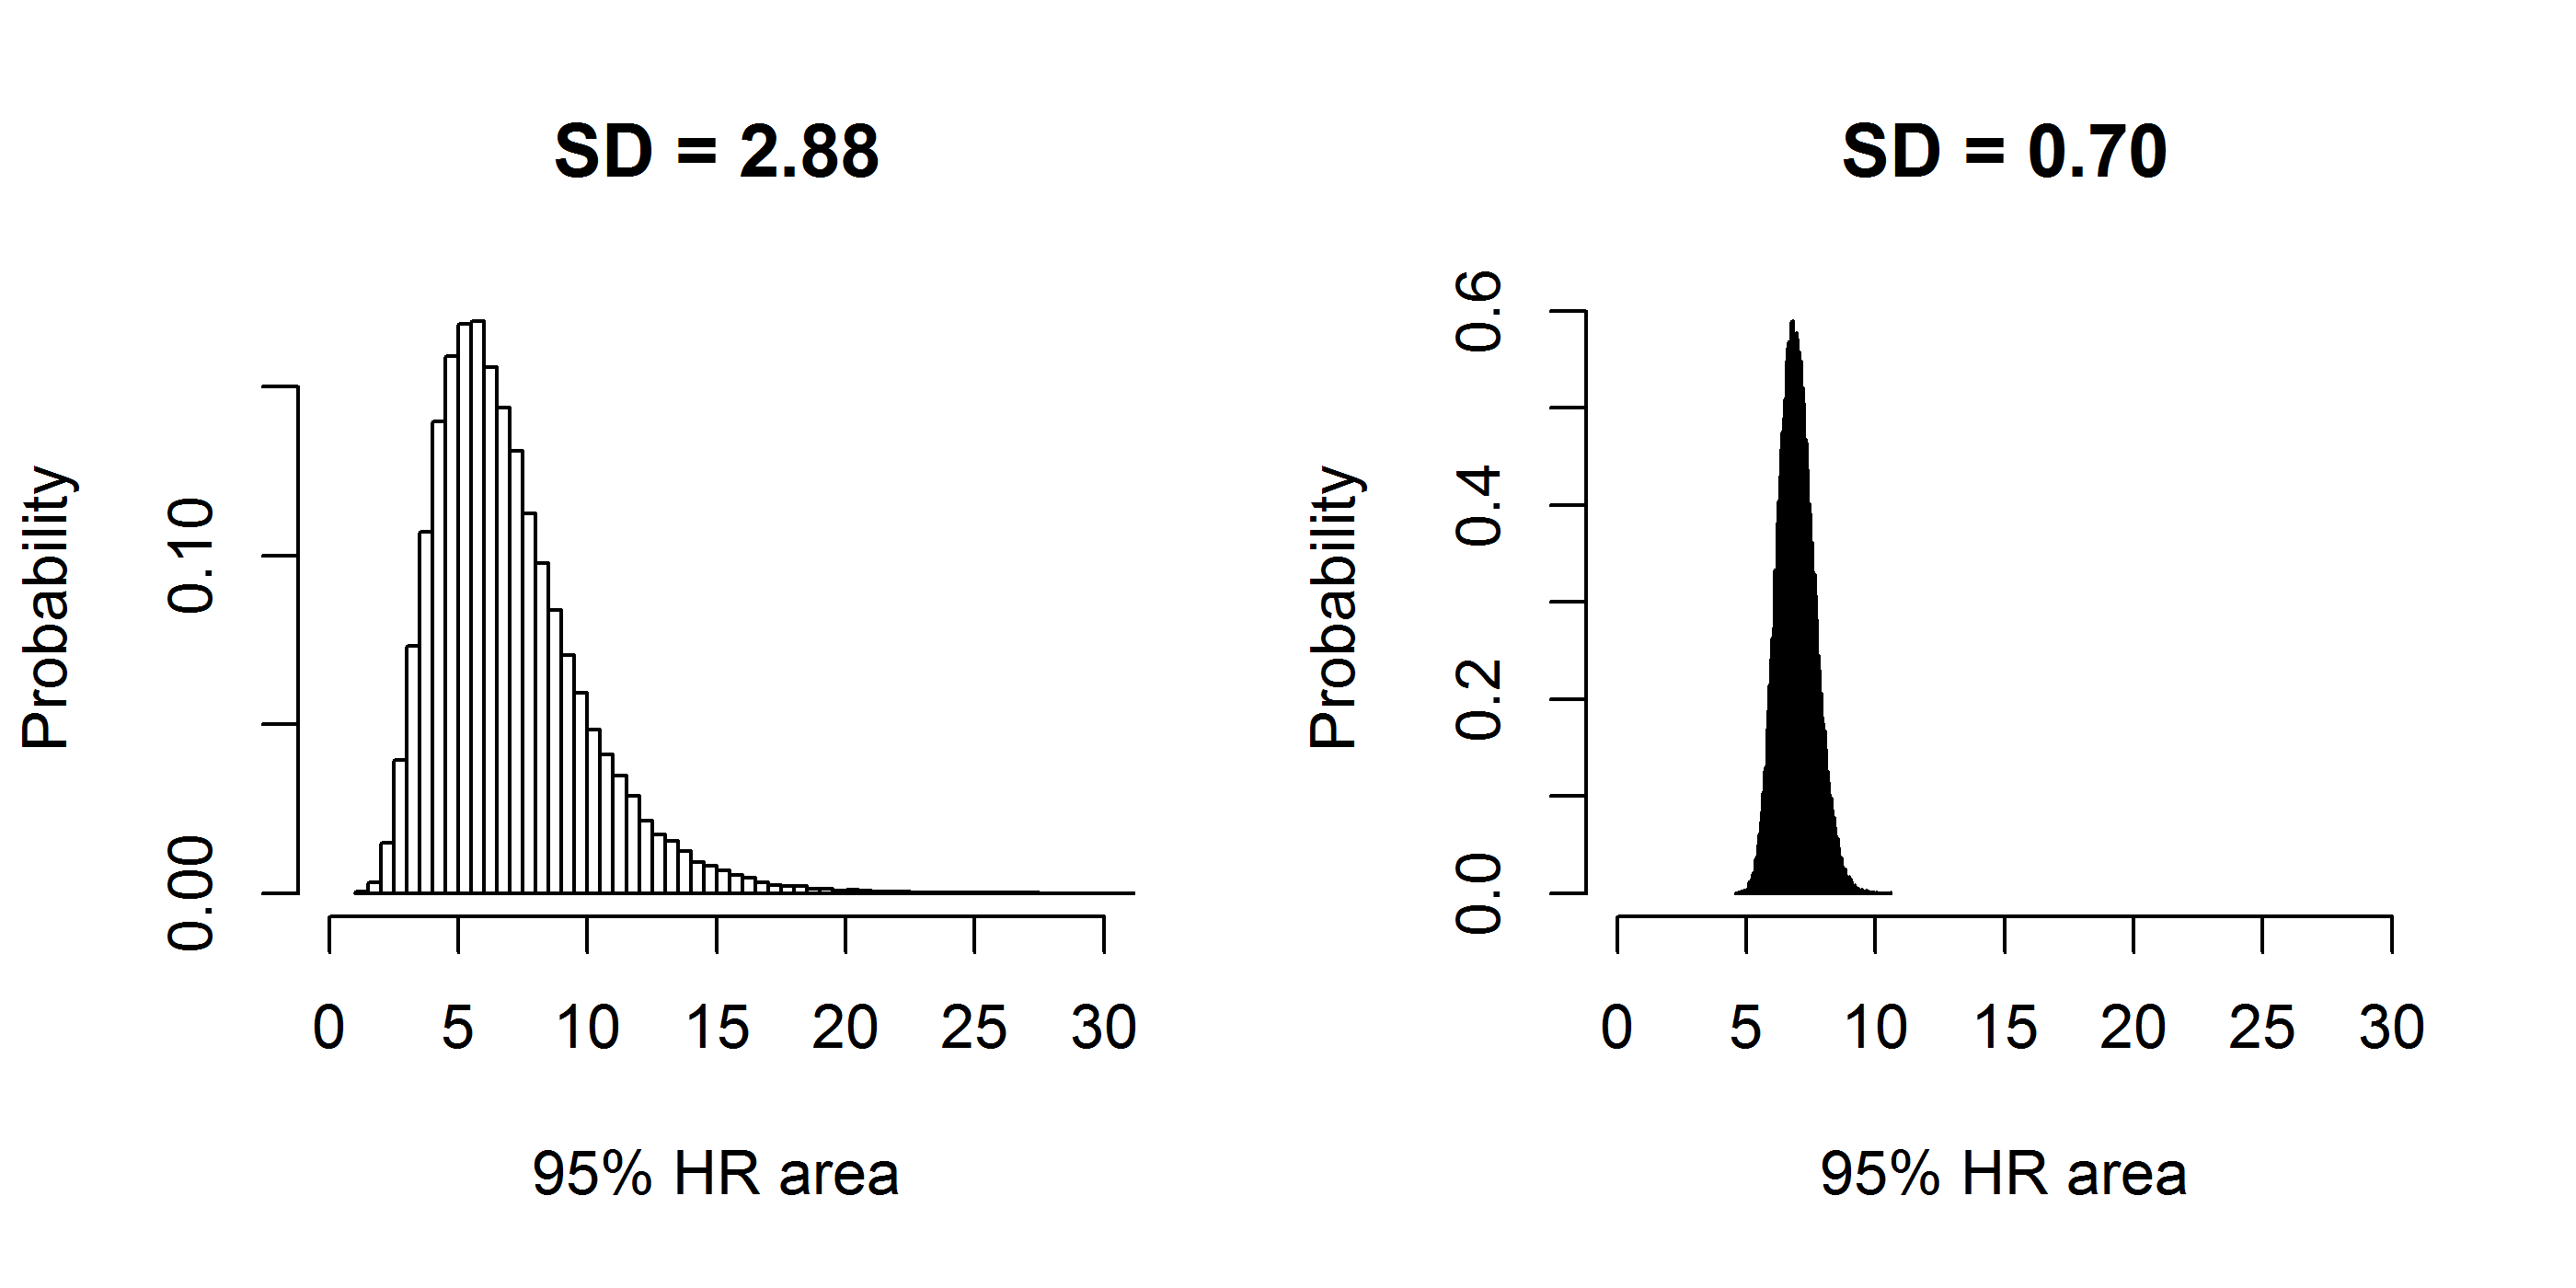
\includegraphics[height=2.5in,width=5in]{Ch8-Covariates/figs/area_heterogeneity.png}
\end{center}
\caption{
Population distribution of home range area for a model in which
$\log(\sigma^{2})$ has a normal distribution with mean $\mu_{hra}$ and
variance $\tau^{2}_{hra}$. The parameters were chosen to yield a
constant expected value of about 6.9 units of area, but to produce two
different levels of heterogeneity: A population standard deviation of
2.88 units (left panel) and 0.70 units (right panel). 
}
\label{covariates.fig.one}
\end{figure}



\section{Likelihood analysis in \secr}
\label{likelihood.secr}

Previously, in Chapt. \ref{chapt.mle}, we introduced the {\bf R}
package \secr~ and described the likelihood based inference approach taken
by that package (see Sec. \ref{mle.sec.secrguts}).  Here we discuss how
to implement some standard covariate models in \secr~ and provide an
example of model selection using AIC.   As we saw in
Chapt. \ref{chapt.mle}, \secr~ uses the standard \R~ model
specification syntax, defining the dependent and independent
variable relationship using tildes (e.g., \Verb+y ~ x+).  Thus, in
\secr~ we might have \verb+g0 ~ behavior+ or
\verb+sigma ~ time+; when left unspecified or set to 1 (e.g.,
\verb+g0 ~ 1+), this will default to a model with no covariates (i.e.,
constant parameter values).  A number of default model formulas for
the baseline and scale parameter of the encounter probability model
are available in \mbox{\tt secr}.
Additionally, \secr~ allows us to specify
covariates on density (we cover this in
Chapt. \ref{chapt.state-space}), which are set for
example as \verb+D ~ habitat+.

To demonstrate
 models with various types of covariates using \secr, we
continue using the Fort Drum black bear data. 
We include in the \scrbook package a function called {\tt secr.bear}
that will format the data (see Chapt. \ref{chapt.mle} for the \secr
data format) and then fit and compare 8 models (details shown in Panel
\ref{covariates.panel.secrfn} ).  We have described all of these
models in the previous sections, so we only briefly comment here on
how to fit certain models in \secr and compare them using AIC, and
give a few helpful notes.
% Below, 
% we have a few subsections on the sex-specific effects, heterogeneity,
% and AIC which describe in more detail how we fit these models within
% \secr.

\subsection{Notes for fitting standard models}

In the \secr package, the encounter probability model is called the
``detection function'' and it is specified 
by changing the ``\mbox{\tt detectfn}'' option (an integer code)
within the \mbox{\tt secr.fit} command.  Table
\ref{covariates.tab.detmodels} shows the possible encounter
probability models 
that \mbox{\tt secr} allows; the default is that based on the kernel
of a bivariate normal probability distribution function
(hence we call this the Gaussian model, but it is referred to as
``half-normal'' 
in \mbox{\tt secr}) and the
(negative) exponential is \mbox{\tt detectfn = 2}.  See model 2 in 
Panel \ref{covariates.panel.secrfn} for how to fit the exponential 
model to the Fort Drum bear dataset. 

The \mbox{\tt secr} package easily fits a range of SCR equivalents of standard capture-recapture models.
The package has pre-defined versions of the classic
model $M_{t}$ where each
occasion has its own encounter
 probability, as well as a linear
trend in baseline encounter probability 
over occasions (in a spatial modeling framework $\sigma$ could also be
an occasion specific parameter, but having encounter probability 
 change with time seems like the more common case). For the classical
time-effects type of model with $K$ distinct parameters \secr~ uses 't' to denote
this in the model specification formula (see model 3 in 
panel \ref{covariates.panel.secrfn}); whereas, for a linear
trend over occasions \secr~ uses 'T'.

The global trap response model (what we called model $M_{B}$), 
or a local trap-specific behavioral response (model $M_{b}$)
can be fitted in \mbox{\tt secr} using formulae with
 ``b'' for the global response model and
 ``bk'' for the local trap response model
(see models 4 and 5 in 
Panel \ref{covariates.panel.secrfn}; note that to fit the trap specific behavioral response model you need version 2.3.1 or newer of \secr).

\begin{panel}[htp]
\centering
\rule[0.1in]{\textwidth}{.03in}
{\small
\begin{verbatim}
1. null model with a bivariate normal encounter probability  model
bear_0=secr.fit(bear.cap, model=list(D ~ 1, g0 ~ 1, sigma ~ 1))

2. null model with an exponential encounter probability model
bear_0exp=secr.fit(bear.cap, model=list(D ~ 1, g0 ~ 1, sigma ~ 1),
          detectfn=2)

3. model with fixed time effects
bear_t=secr.fit(bear.cap, model=list(D ~ 1, g0 ~ t, sigma ~ 1))

4. global behavioral model
bear_B=secr.fit(bear.cap, model=list(D ~ 1, g0 ~ b, sigma ~ 1))

5. trap specific behavioral response
bear_b=secr.fit(bear.cap, model=list(D ~ 1, g0 ~ bk, sigma ~ 1))

6. global behavior model with fixed time effects
bear_bt=secr.fit(bear.cap, model=list(D ~ 1, g0 ~ b+t, sigma ~ 1))

7. sex-specific model
bear_sex=secr.fit(bear.cap, model=list(D ~ session, g0 ~ session, 
         sigma ~ session))

8. heterogeniety model
bear_h2=secr.fit(bear.cap, model=list(D ~ 1, g0 ~ h2, sigma ~ h2))
\end{verbatim}
}

\rule[-0.1in]{\textwidth}{.03in}
\caption{
Models called from \mbox{\tt secr.bear} function. All models use \mbox{\tt buffer = 20000}}
\label{covariates.panel.secrfn}
\end{panel}


\subsection{Sex Effects}
\label{covariates.secr.sex}

Incorporating sex effects into
models with \secr~ can be done a few different ways, but there are not
pre-defined models for this.  A limitation of fitting models with sex
effects in \mbox{\tt secr} is that it does not accommodate missing
values of the sex variable. Thus, in all cases,
individuals that are of unknown sex must be removed from the dataset
(recall that in a Bayesian framework we can keep these individuals in
the data set by specifying a distribution for the individual covariate
``sex'').
In \mbox{\tt secr}, the easiest way to include sex effects is 
to code sex as a  ``session'' variable using the multi-session models
(see Sec. \ref{mle.sec.multisession} for a description
of the multi-session models), providing two sessions, one representing
males and one for females (see model 7 in Panel
\ref{covariates.panel.secrfn}).  This method provides two separate
density estimates, which can then be combined into a total density.

\begin{comment}
There are a few ways that one could
specify the model with sex-specific parameters  in \mbox{\tt secr} (M. Efford, pers. comm).  One way is that we could
list sex as a categorical individual covariate in a Huggins-Alho type
model \citep{borchers_efford:2008}.
 A similar approach is to treat males and 
females as groups (in \secr~ denoted by ``g''), specify the
model as $model = list(D~g, g0~g, \sigma~g)$ and list \mbox{\tt groups = 'sex'}
where we have specified sex as a 2-level individual covariate.    The \secr~ manual suggests that for many purposes,
using the `session' implementation is equivalent to the 'groups' with the caveat that the latter is often simpler
to implement partially due to the fact that multi-session models require the detector array and mask to be 
specified separately for each session.
\end{comment}


\subsection{Individual heterogeneity}
\label{covariates.sec.secrH2}

To incorporate heterogeneity, \secr fits a set of 
finite mixture models \citep{norris_pollock:1996,
  pledger:2000}. These are expensive in terms of parameters but 
they have been widely adopted because they are easy to analyze using
likelihood methods, as the marginal distribution of the data is just a
sum of a small number of components.
Using \secr,  individual heterogeneity can be incorporated
into the encounter probability model using default models for 
 either a 2- or 3-component finite
mixture model 
using the  ``\mbox{\tt h2}'' or
``\mbox{\tt h3}'' model terms.
 The 2-part mixture is shown in model 8 of panel
\ref{covariates.panel.secrfn} and the 3-part mixture can easily be fit by
substituting \mbox{\tt h3} for \mbox{\tt h2}.  
The finite-mixture model 
can be fit in \jags~ or \bugs, but we only showed
the SCR + Mh logit-normal mixture in the version above (see
Sec. \ref{covariates.sec.heterogeneity}).



\subsection{Model selection in \secr~ with AIC}

One practical advantage to using the \secr~ package, or likelihood
inference in general, is the convenience of automatic model selection
using AIC \citep{burnham_anderson:2002}. The \mbox{\tt secr} package
has a number of convenient functions for computing AIC and producing
model selection tables, or doing model-averaging (as described in
 Chapt. \ref{chapt.gof}).
Running the function {\tt secr.bear}, which calls all of the models we
have described, will return, in addition to all model results, 
an AIC table with all of the summarized results including the AIC values,
delta AIC, and model weights (see Table \ref{covariates.tab.secrAIC}
or reproduce results in {\tt R} using {\tt out<- secr.bear(); out\$AIC.tab}). 


It is important to note that AIC is not comparable 
between a multi-session model and a model that is not a multi-session model.
Therefore, to compare the sex-specific model (which uses ``sessions") with all the other models
including the null, time, and behavioral models, we coded the dataset as a 
multi-session design when first loading it to \secr.  This results in 
all the model outputs listing separate parameter estimates for each session, even the null model
with no covariates; however, the estimates are the same for both ``sessions''
in all but the sex specific model. 


\begin{table}[ht]
\centering
\caption{Log-likelihood, AIC, deltaAIC and AIC weight for several models run in secr for the Fort Drum black bear data set.}
\begin{tabular}{crrrrr}
\hline \hline
model     &  logLik   &   AIC    &   AICc   & dAICc  & AICwt \\ \hline
bear.b    & -641.7215 & 1291.443 & 1292.395 & 0.000  &  1 \\
bear.h2   & -653.8382 & 1319.676 & 1321.776 & 29.381 &  0 \\
bear.0exp & -663.9152 & 1333.830 & 1334.389 & 41.994 &  0 \\
bear.B    & -677.6175 & 1363.235 & 1364.187 & 71.792 &  0 \\
bear.bt   & -668.3044 & 1358.609 & 1366.152 & 73.757 &  0 \\
bear.sex  & -677.7151 & 1367.430 & 1369.530 & 77.135 &  0 \\
bear.t    & -674.4134 & 1368.827 & 1374.938 & 82.543 &  0 \\
bear.0    & -686.2455 & 1378.491 & 1379.049 & 86.654 &  0 \\ \hline
\end{tabular}
\label{covariates.tab.secrAIC}
\end{table}


The results from this AIC analysis are straightforward to interpret; the model
with a local trap response of encounter probability, ``bk'', has a model weight of 1 and thus, according to AIC, 100\% support.
The 2-part finite mixture model for $g_0$ and $\sigma$ has the second lowest
AIC, but considering the large dAICc compared to the local trap response model we would probably not consider it any further.  
% Using the AIC provides a fast and convenient mechanism for
% conducting model comparisons. 


\section{Summary and Outlook}

There are endless covariates and encounter probability models that can
be defined and our goal in this chapter was to introduce basic types
of covariate models and demonstrate how to implement them in {\bf
  BUGS} and \mbox{\tt secr}.  Essentially, SCR's are GLMMs and
therefore we develop covariate models in much the same way, using a
suitable transformation (link function) of the parameter(s). In SCR
models, we typically have 2 parameters of the encounter probability
model for which we might specify covariate models -- the baseline
encounter probability (or rate) parameter, and a scale parameter that
is related in many cases to the home range size of the species.  A few
examples of different covariate models are given in Table
\ref{covariates.tab.covclass}.  We can also consider covariates by
their classification as fixed, partially observed, or unobserved (see
Table \ref{covariates.tab.covobs}). This classification of covariate
types can be important because the MLE and Bayesian approaches to
dealing with partially and unobserved covariates is often different.
This was seen above in how the covariate \mbox{\tt Sex} was handled in
the two frameworks.

\begin{table}[ht]
\centering
\caption{Examples of different covariate classifications.}
\begin{tabular}{cr}
\hline \hline
Covariate class & Examples \\
\hline 
Fixed & baited, weather, habitat\\
Partially observed & sex, age, \\
Unobserved &  home range size, ind. effects  \\ \hline
\end{tabular}
\label{covariates.tab.covobs}
\end{table}

While the move to spatially explicit models in capture-recapture
studies has largely rendered the basic CR models
\citep{otis_etal:1978} obsolete, we continue to find this
classification useful for categorizing the {\it spatial} extensions of
these standard CR models.  The extended models include the standard
$M_0$, $M_t$, $M_b$, and $M_h$, but also new models that allow for
trap-specific information such as "baited/not-baited" or "on/off
road".  In addition, in Chapts. \ref{chapt.ecoldist}, \ref{chapt.rsf}
and \ref{chapt.state-space}, we explore additional models for
explaining variation in encounter probability and density based on
spatial covariates that describe variation in landscape or habitat
conditions.

%Researchers are often concerned with describing the factors or
%covariates that influence variation in detection or encounter
%probability, particularly as this can directly influence other
%parameters in the model such as density.  These covariates have
%various levels -- specific to individual, trap, sampling occasion and
%can be fully or partially observed as well as completely latent.  In
%SCR models, these more complex covariate models are fairly easy to
%fit, though one should take caution not to over parameterize the
%models particularly when a study yields a sparse data set.


\begin{comment}
Different detection models: We can make up detection models {\it all fucking
day}, to no end, with no point, and with no biological justification for
any single model. To us this would be bad practice and so we think it is
perfectly fine to pick a model ahead of time and stick with it.

we note that underlying these different models is basically something
to do with the 2nd moment structure of some correlated spatial process...
i.e., correlation functions (Higdon et al. 1998; etc...) and , insofar
as choosing detection functions is like choosing a correlation function,
it probably wont have much affect on inferences.
\end{comment}


\begin{comment}
XXXX Andy sez: probably not -- we can stop here at a basic
description of the models XXXX

XXX Andy, do you still think this is necessary? XXX
It is interesting to consider alternative distributions for $\alpha_{1,i}$, here we 
use a Normal prior which might result in a negative value for $\alpha_{1,i}$ which is
not expected but also not entirely nonsensical.  We could also use the the Inverse-Gamma
distribution, but it is not conjugate in the present context and so
there is no compelling reason to do that.  Also important to note is that if A[i] 
is the home range area of individual $i$, and we have related area to $\sigma$ through a specified
function, then we can move back and forth between distributions for
A[i], $\sigma_i$, and $\alpha_{1,i}$.


{\bf Approximation: }
Note that ``SCR + Mh'' might be a good approximation to ``SCR + Ah''.  If we write $\alpha_{1,i} =
\alpha_{1} + \eta_{i}$ then
we can take the expectation over  $\alpha_{i}$ to arrive at
\[
\mbox{logit}(p0) = \alpha_0 
p_{ijk} = p0 \exp(- \alpha_{1}*||{\bf s}_{i}-{\bf x}_{j}||^2) +  \eta_{i}*||{\bf s}_{i}-{\bf x}_{j}||^2)
\]

Which has this additive individual effect that varies also by trap. It might be that approximating
this by SCR+Mh is better than nothing and it could also be viewed as suggesting an 
over-dispersed count model for encounter frequencies.

XXXXXXXXXXXXXXXXX above commented out 

\end{comment}
%\chapter{Modeling Encounter Probability}
%\label{chapt.covariates}

%\chapter{Goodness of Fit and stuff}
%\label{chapt.gof}
\chapter{
Model Selection and Assessment
}
\markboth{Model Assessment}{}
\label{chapt.gof}

\vspace{.3in}

% XXXX Great opener XXXX
Our purpose in life is to analyze models. By that, we mean one or more
of the following basic 4 tasks: (1) estimate parameters, (2) make predictions
of unobserved random variables, (3) evaluate the
relative merits of different models or choosing a best model (model
selection), and (4)  checking whether a specific model appears to provide a
reasonable description of the data or not (model checking, assessment,
or ``goodness-of-fit'').  In previous chapters we
addressed the problems of estimation of model parameters, 
and also making
predictions of latent variables, ${\bf s}$ or $z$, or
functions of these variables such as density or population size.
In this chapter, we focus on the last two of these basic
inference tasks: model selection (which model or models should be
favored), and model assessment (do the data appear to be consistent
with a particular model).


In this chapter we review  basic strategies of model selection 
using both likelihood methods (as
implemented in the \mbox{\tt secr} package) and Bayesian
analysis.
Specifically,
we review a number of standard methods of model selection that apply
to ``variable selection'' problems, when our set of models
consists of distinct covariate effects and they represent constraints
of some larger model.
For classical analysis based on likelihood, model selection by Aikaike Information
Criterion (AIC) is the standard approach \citep{burnham_anderson:2002}.  For
Bayesian analysis we rely on a number of different methods.  We
demonstrate the use of the deviance information criterion (DIC)
\citep{spiegelhalter_etal:2002} for variable selection problems
although it has deficiencies when applied to hierarchical models in
some cases \citep{millar:2009}. 
We use the
Kuo and Mallick indicator variable selection approach
\citep{kuo_mallick:1998} which
produces direct statements
of posterior model probabilities which we think are the most useful,
and leads directly to model-averaged estimates of density.  There is a
good review paper recently by \citet{ohara_sillanpaa:2009} that discusses
these and many other related ideas for variable selection.
 In addition to \citet{ohara_sillanpaa:2009} we
also recommend \citet[][Chapt. 7]{link_barker:2010} for general
information on model selection and assessment.

 To check model adequacy in a Bayesian framework, or whether a
specific model provides a satisfactory description of our data set,
we rely exclusively on the Bayesian
p-value framework \citep{gelman_etal:1996}.  For assessing fit of 
SCR models, part of the challenge is coming up with good measures of
model fit, and there does not appear much definitive guidance 
in the literature on this point.  Following \citet{royle_etal:2011mee}, we break the
problem up into 2 components which we attack separately: (1)
Conditional on the underlying point process, does the encounter model
fit? (2) Do the uniformity and independence assumptions appear
adequate for the point process model of activity centers? The latter
component of model fit has a considerable precedence in the
ecological literature as it is analogous to the classical problem of
testing ``complete spatial randomness'' \citep{cressie:1992, illian_etal:2008}.


We apply some of these methods to the wolverine camera trapping
data first introduced in Chapt. \ref{chapt.scr0}
to investigate sex specificity of model parameters and whether
there is a behavioral response to encounter. We note that individuals
are drawn to the camera trap devices by bait and therefore it
stands to reason that once an individual discovers a trap, it  might
be more likely to return subsequently, a response termed
``trap happiness". We evaluate whether certain models for encounter
probability  appear to be
adequate descriptions of the data, and we evaluate the uniformity
assumption for the underlying point process.



\begin{comment}
A basic problem with these two objectives of model selection and model
assessment is their simultaneous use implies a kind of contradiction
which we call the {\it model selectors paradox}: Inferences are always
achieved using standard paradigms of parametric inference (Bayesian or
% XXXX Perhaps we should be open to non-parametric methods. Bob
% Dorazio seems to interested in non-parameteric approaches.
frequentist) which assert that the model is properly specified. That
is, we assume that the model is truth. This is paradoxical because we
all know that ``all models are wrong'' but, possibly, ``some are
useful.'' In fact, the notion that an ``assumption'' could even be
correct is itself something of an oxymoron.
\end{comment}

\begin{comment}
%XXX I love this quote -- would be nice to use it somewhere: XXXX
  Therefore we don't expect
or hope to make assumptions that are ``correct'' in any way. Gelman
and Shalizi (2010) say it this way: ``there is general agreement that,
in this domain, all models in use are wrong -- not just merely
falsifiable, but actually false.''  We should therefore refrain from
over-stating the relevance of any model.  [not sure where I was going
with this point]
\end{comment}



% XXXX Suggest un-commenting this material
\begin{comment}
A few specific questions to resolve:
\begin{itemize}
\item[(1)]  Can AIC or DIC choose among detection models and does it matter?
\item[(2)]  Can AIC or DIC choose among more substantial models?  We should
 assume it does. Can we rig up a test?  Suggest: (1) trap level
 covariate and trying DIC; (2) Model Mb vs. not
\item[(3)] Simultaneous to above, see if we can do that.......
Posterior model probabilities: Can we demo this?   With detection models?
 Don't do much analysis of the situation, just demo it maybe?
\item[(4)]  Basic framework for Bayesian GoF. Power under alternatives.
(clustering, regularity, uniformity) and misspecified encounter models
-- do they show a lack of fit?
\end{itemize}
\end{comment}



\begin{comment}
\subsection{The Role of model assumptions}

{\bf XXXXX NOTE THIS IS COMMENTED OUT XXXXXXXXXXXXXXXXXXXXXXXXXXX}

Referees are quick to point out that bivariate normal distributions as
models for home range are simply wrong. As if using wrong models
somehow invalidates something. (is that a statistical paradigm that I
missed?). The issues are whether its an adequate model, whether we can
refute it, whether resulting inferences are sensitive to it, and
whether the model is useful for its intended purpose regardless.
If  we really wanted a great description of a home range then we would do
something different besides conduct an SCR study. The purpose of most
SCR models is not to study home range geometry and morphology but, rather,
to estimate density and possibly other vital rates such as survival and
recruitment. In addition, it is my experience that the same people who
criticize models as implying overly simple models actually cannot describe
alternative models except using jargon and procedures like "kernel
smoothing", "utilization distributions" and "neural networks". So, on
the one hand, the bivariate normal distribution is overly simple, and
therefore we should use "neural networks"?  What irritates me even more
is referees who emphatically assert that "real home ranges aren't bivariate
normal" and then they go on to cite references who somehow "proved" they
are not. These people have no clue what statistics is good for and what
the point of SCR models is, nor can they grasp the relevance of the home
range model - namely, as a model for explaining heterogeneity in
capture-probability. To be sure, the bivariate normal model is an
over-simplification but so far it has not been shown to be ineffective
in SCR problems, and besides  substantially more flexible models have been
developed \citep{royle_etal:2012ecol}.

What we care about in models of capture-recapture data is whether the
bivariate normal (or any model) provides an adequate description of the
encounter process. That is the question we will evaluate here.
\end{comment}





\begin{comment}

%\section{Strategies for Model Selection}

We review a number of standard methods of model selection that apply
to ``variable selection'' problems. That is, when our set of models
consists of distinct covariate effects and they represent constraints
of some larger model.
For classical analysis based on likelihood, model selection using 
the Akaike information criterion (AIC)
is the standard approach \citep{burnham_anderson:2002}.  For
Bayesian analysis we rely on a number of different methods.  We
demonstrate the use of the deviance information criterion (DIC)
\citep{spiegelhalter_etal:2002} for variable selection problems
although it has deficiencies when applied to hierarchical models in
some cases \citep{millar:2009}. 
We use the
Kuo and Mallick indicator variable selection approach
\citep{kuo_mallick:1998} which
produces direct statements
of posterior model probabilities which we think are the most useful,
and leads directly to model-averaged estimates of density.  There is a
good review paper recently by \citet{ohara_sillanpaa:2009} that hits
on these and many more related ideas for variable selection.
 In addition to \citet{ohara_sillanpaa:2009} we
also recommend \citet[][Chapt. 7]{link_barker:2010} for general
information on model selection and assessment.

%  We have not done a comprehensive evaluation of different methods for
%  effect and efficiency.

\end{comment}

\begin{comment}
\subsection{Scope of the model selection problem}

There are two distinct classes of problems that we encounter in SCR
models which might require some type of model selection or ranking
effort: (1) Choosing among models that represent distinct, meaningful
biological hypotheses; and, (2) choosing among different parametric
encounter probability models. We believe that the importance of model
selection depends on which type of problem we have.

{\flushleft {\bf Choosing among biological models:}}
SCR models that represent extensions of the basic null model by
including specific covariates or other effects often represent
explicit biological hypotheses. Examples include models with a
behavioral response, or seasonal variation in encounter probability,
or sex-specificity of model parameters.
We anticipate that such basic biological factors
could be important, and therefore it can be useful to choose among (or
rank) a set of models that represent these hypotheses.

{\flushleft {\bf Choosing among models for encounter probability:}} In
Sec. \ref{scr0.sec.implied} we introduced the notion that encounter
probability models imply specific models of space usage, an idea we
expand on and generalize in Chapt. \ref{chapt.rsf}. Because of this
linkage between the model for encounter probability and space usage,
it is tempting to want to choose among the models believing them to be
biological models.  Our feeling is that
% XXXX Should we say "most" enc models are not biologiacal constructs?
% Otherwise it seems as though we are having it both
% ways. i.e. sometimes we think they are related to movement, and
% sometimes not. Also, Murray has a few models that allow for "sound
% attenuation due to spherical spreading" XXXX
the encounter probability
models are not biological constructs (not motived by biological
considerations) but, rather, purely phenomenological descriptions of
home range. Moreover, as the standard models are all stationary and
isotropic they are simply unrealistic models. Therefore, it seems to
us that choosing among a dozen or more arbitrary parametric forms that
have no biological motivation should tend to lead to an over-fitting.
So we will apply ideas of model selection to some problems below (and
elsewhere in this book) but we avoid the problem of choosing among
detections functions and we discourage people from doing that.
\end{comment}



\section{Model Selection by AIC}
\label{gof.sec.aic}

Using classical analysis based on likelihood, model selection
is easily accomplished using AIC \citep{burnham_anderson:2002}
which we demonstrate below. The AIC of a model is simply twice the
negative log-likelihood evaluated at the MLE, penalized by the number of parameters
($np$) in the model:
\[
 \mbox{AIC} = -2 \mbox{logL}(\hat{\bm \theta}|{\bf y})  + 2 np
\]
Models with small values of AIC are preferred.
It is common to use a modified (``corrected'') AIC referred to as $AIC_{c}$ for small
sample sizes which is
\[
 \mbox{AIC}_{c}  =
-2 \mbox{logL}(\hat{\bm \theta}|{\bf y})  + \frac{2 np
  (np+1)}{n-np-1}
\]
where $n$ is the sample size.  Two important problems with the use of
AIC and AIC$_{c}$ are that they don't apply directly to hierarchical
models that contain random effects, unless they are computed directly
from the marginal likelihood (for SCR models we can do this, see
Chapt. \ref{chapt.mle}). Moreover, it is not clear what should be the
effective sample size $n$ in calculation of AIC$_{c}$, as there can be
covariates that affect individuals, that vary over time, or space.
We do not offer strict guidelines as to when to use a small sample
size adjustment.

The {\bf R} package \mbox{\tt secr} computes and outputs AIC
automatically for each model fitted and it provides some capabilities
for producing a model selection table (function \mbox{\tt AIC}) and
also doing model-averaging (function \mbox{\tt model.average}), which
we recommend for obtaining estimates of density from multiple models.

\subsection{AIC analysis of the wolverine data}

We provide an example of model selection for the wolverine camera
trapping data using \mbox{\tt secr}.
 We consider a model set with  distinct models to accommodate
various types of sex specificity of model parameters:
\hspace{.5in} \begin{itemize}
\item[] Model 0: model SCR0 with constant density and constant
  encounter model parameters;

\item[] Model 1: model SCR0 with constant parameter
values for both male and female wolverines but with sex-specific
density only;

\item[] Model 2: Sex-specific density, sex-specific $p_{0}$ but constant $\sigma$;

\item[] Model 3: Sex-specific density, sex-specific $\sigma$ but constant
$p_{0}$;

\item[] Model 4: Sex-specific density, sex-specific $p_{0}$ and sex-specific $\sigma$.
\end{itemize}

To model sex-specific abundance (density), we  use the multi-session models  provided by
\mbox{\tt secr} (introduced in Sec. \ref{mle.sec.multisession}), which
allow one to model session-specific effects on density, baseline
encounter probability, $p_{0}$ (labeled $g_{0}$ in \mbox{\tt secr}), and also the scale
parameter $\sigma$ of the encounter probability model. Using this
formulation, we define the ``Session'' variable to be a {\it
  categorical} sex code having value 1 or 2 (demonstrated below) and
thus {\it session}-specific parameters represent {\it sex}-specific parameters.
For example, if we model session-specific density, $D$, then this
corresponds to Model 1 in our list above.  We note that ``Model 0'' in
our list corresponds to a model where all of the encounter
histories have the same session ID. This model is one of constant
density, which implies that the population sex ratio is fixed at 0.5, i.e.,
$\psi_{sex} = 0.5$. 

\begin{comment}

% XXX moved this section to the BUGS section
For fitting these models in {\bf BUGS} we use dummy variables. We
model  covariates on $p_{0}$ on
the logit-scale, and covariates on $\sigma$ on the
log-scale.
 Thus,  we will express  models allowing for sex-specificity
using a dummy variable \mbox{\tt Sex} and new parameters
($\alpha_{sex}$, $\beta_{sex}$) which
represent the {\it effect} of \mbox{\tt Sex} at level 1:
\[
 \mbox{logit}(p_{0,i}) = \alpha_{0} + \alpha_{sex} \mbox{\tt Sex}_{i}
\]
and
\[
 \mbox{log}(\sigma_{i}) = \log(\sigma_{0}) + \beta_{sex} \mbox{\tt Sex}_{i}
\]
In these expressions, the sex variable $\mbox{\tt Sex}_{i}$ is a
binary variable where $\mbox{\tt Sex}_{i}= 0$ corresponds to female,
and $\mbox{\tt Sex}_{i} = 1$ corresponds to male. 

\end{comment}

Although \mbox{\tt
  secr} also uses the logit/log linear predictors as the default for
modeling covariates on baseline encounter probability and the scale
parameter, respectively, \mbox{\tt secr} does something different with
the multi-session models. It reports estimates in a {\it session mean}
parameterization (equivalent to, in {\bf BUGS}, using an index
variable instead of a set of dummy variables), and not the {\it
  session effect} (i.e., deviation from the intercept) which arises
from the use of dummy variables.  We show this \bugs~ model description 
in Sec. \ref{gof.sec.dicwolverine}. 


To fit these models using \mbox{\tt secr}, 
we load the wolverine data and do 
a slight bit of formatting to prepare the data objects for analysis by
\mbox{\secr}. The key difference from our analysis in
Chapt. \ref{chapt.mle} is, here, we use the wolverine sex information
(\mbox{\tt wolverine\$wsex}) which is a binary 0/1 variable (1=male) 
and we add
1 so that we can define a categorical  ``Session'' variable (having
values 1 or 2). We also have a function \mbox{\tt scr2secr} which
converts a standard trap-deployment file (TDF) matrix into a \mbox{\tt secr}
object of class ``\mbox{\tt traps}.''
The {\bf R} commands are as follows (contained in the help file
\mbox{\tt ?secr\_wolverine}): 
% XXXX Should we try to force R code chunks to be on 1 page? If so,
% there is a "samepage" environement that does this, but it seems to
% occassionally create odd-looking spacing.
{\small
\begin{verbatim}

> library(secr)
> library(scrbook)
> data(wolverine)
> traps <- as.matrix(wolverine$wtraps)

## Name variables as required by secr
> dimnames(traps) <- list(NULL,c("trapID","x","y",paste("day",1:165,sep="")))
## Convert trap information to a secr "traps" object
> trapfile <- scr2secr(scrtraps=traps,type="proximity")

## Grab the wolverine state-space grid (2km here)
> gr <- as.matrix(wolverine$grid2)
> dimnames(gr) <- list(NULL,c("x","y"))
> gr2 <- read.mask(data=gr)

## Grab the encounter data, and re-name variables
> wolv.dat <- wolverine$wcaps
> dimnames(wolv.dat) <- list(NULL,c("Session","ID","Occasion","trapID"))

## Convert binary 0/1 sex variable to categorical 1/2 for "session"
> wolv.dat[,1] <- wolverine$wsex[wolv.dat[,2]]+1
> wolv.dat <- as.data.frame(wolv.dat)

## Convert to capthist object
> wolvcapt <- make.capthist(wolv.dat,trapfile,fmt="trapID",noccasions=165)
\end{verbatim}
}

Once the data have been prepared in this way, we use the
\mbox{\tt secr} model fitting function \mbox{\tt secr.fit} to fit the
different models, and then the function \mbox{\tt AIC} to
package the models together and summarize them in the form of an AIC
table, with rows of the table ordered from best to worst. The function
\mbox{\tt model.average} performs AIC-based model-averaging of the
parameters specified by the \mbox{\tt realnames} variable (below this
is demonstrated for the parameter density, $D$).  Because this
% XXXX Earlier, AIC was in math-mode. Should we stick with $AIC_c$?
function defaults to averaging by AIC$_c$, we slightly modified
this function (called \mbox{\tt model.average2}) to do model averaging
by either  AIC or AIC$_c$ as specified by the user. The model fitting
commands look like this (for Model 0 and Model 1):
{\small
\begin{alltt}
> model0 <- secr.fit(wolvcapt, model=list(D\(\sim\)1, g0\(\sim\)1, sigma\(\sim\)1), 
                  buffer=20000)
> model1 <- secr.fit(wolvcapt, model=list(D\(\sim\)session, g0\(\sim\)1, sigma\(\sim\)1), 
                  buffer=20000)
\end{alltt}
}
Next we use the function \mbox{\tt AIC}, passing the fit objects from
all 5 models, and that produces the following output (abbreviated
horizontally to fit on the page):
{\small
\begin{verbatim}
> AIC (model0,model1,model2,model3,model4)
            model         ... npar  logLik    AIC     AICc dAICc  AICwt
model0  D~1 g0~1 sigma~1  ...  3 -627.2603 1260.521 1261.932 0.000 0.5831
model2      ..            ...  5 -624.9051 1259.810 1263.810 1.878 0.2280
model1      ..            ...  4 -627.2365 1262.473 1264.973 3.041 0.1275
model4      ..            ...  6 -624.6632 1261.326 1267.326 5.394 0.0393
model3      ..            ...  5 -627.2358 1264.472 1268.472 6.540 0.0222
\end{verbatim}
}
Model averaging the results is done as follows:
{\small 
\begin{verbatim}
> model.average (model0,model1,model2,model3,model4,realnames="D")
              estimate  SE.estimate          lcl          ucl
session=1 2.707190e-05 7.913577e-06 1.544474e-05 4.745224e-05
session=2 2.927423e-05 8.270402e-06 1.700631e-05 5.039193e-05
\end{verbatim}
}
As usual, estimates and standard errors of the individual model
parameters can be obtained from the \mbox{\tt secr.fit} summary output
of any of the \mbox{\tt modelX} objects shown above.
The default output of estimated density is in individuals per ha, so
we have to scale this up to something more reasonable. To get into
units of per 1000 km$^2$, we need to first multiply by 100 to get to units of
km$^2$ and then multiply by 1000. This produces an estimated density of
about 2.71 for \mbox{\tt session=1} (females) and 2.93 for
\mbox{\tt session=2} (males).  We can use the generic {\bf R} function
\mbox{\tt predict} applied to the \mbox{\tt secr.fit} output to obtain
 specific information about the MLEs on the natural scale.

 We don't necessarily agree with the use of AIC$_c$ here and think its
 better to use AIC, in general. This is because, as noted previously,
 it is not clear what the effective sample size is for most
 capture-recapture problems. While we have 21 individuals in the data
 set, most of the model structure has to do with encounter probability
 samples and for that there are hundreds of observations. We do note
 that the AIC and AIC$_c$ results are not entirely consistent.  By
 looking at the best model by AIC (Table \ref{gof.tab.aic}), we find
 that the model with sex specfic density and sex specific baseline
 encounter probability, $p_{0}$, is preferred (Model 2). This is just
 slightly better than the null model (Model 0) with no sex effects at all
 and hence an implied fixed sex ratio of $\psi_{sex} = 0.50$).


\begin{table}[ht]
\centering
\caption{
  Model selection results for the  wolverine models of sex-specificity,
  with/without habitat mask.  Fitting was done 
  using  \mbox{\tt secr} with a half-normal (Gaussian) encounter probability
  model. Models are ordered by
  $AIC$. Density, $D$, is
  reported in units of individuals per 1000 km$^2$. Model abbreviations
  indicate which parameters are sex-specific in order $D/p_{0}/\sigma$.
}
\begin{tabular}{lccccccccc}
\hline \hline
\multicolumn{10}{c}{NO HABITAT MASK} \\ \hline
        &      &     &      & \multicolumn{3}{c}{Female} & \multicolumn{3}{c}{Male} \\ 
  model & npar & AIC & AICc & D & $p_0$ & $\sigma$ & D & $p_0$ &  $\sigma$  \\ \hline
2: sex/sex/1    &  5&  1259.8& 1263.8 &2.45& 0.08& 6435.51& 3.16& 0.04& 6435.51\\
0: 1/1/1        &  3&  1260.5& 1261.9 &2.83& 0.06& 6298.66& 2.83& 0.06& 6298.66\\
4: sex/sex/sex  &  6&  1261.3& 1267.3 &2.59& 0.08& 6080.70& 2.99& 0.04& 6833.16\\
1: sex/1/1      &  4&  1262.5& 1265.0 &2.69& 0.06& 6298.69& 2.96& 0.06& 6298.69\\
3: sex/1/sex    &  5&  1264.5& 1268.5 &2.70& 0.06& 6280.49& 2.95& 0.06& 6319.03\\
\hline \hline
\multicolumn{10}{c}{WITH HABITAT MASK} \\ \hline
        &      &     &      & \multicolumn{3}{c}{Female} & \multicolumn{3}{c}{Male} \\ 
  model & npar & AIC & AICc & D & $p_0$ & $\sigma$ & D & $p_0$ &  $\sigma$ \\ \hline
2: sex/sex/1   &  5& 1268.1& 1272.1 &  3.64& 0.07& 6382.88& 4.73& 0.03& 6382.88 \\
4: sex/sex/sex &  6& 1268.7& 1274.7 &3.87& 0.07& 5859.40& 4.41& 0.03& 7039.09\\
0: 1/1/1       &  3& 1271.2& 1272.6 &4.18& 0.05& 6282.62& 4.18& 0.05& 6282.62\\
1: sex/1/1     &  4& 1273.1& 1275.6 &3.98& 0.05& 6282.65& 4.38& 0.05& 6282.65\\
3: sex/1/sex   &  5& 1275.1& 1279.1 &3.93& 0.05& 6357.26& 4.41& 0.05& 6220.22\\
\hline
\end{tabular}
\label{gof.tab.aic}
\end{table}


We fit the same models but now using a modified state-space which
excludes the ocean (this is a habitat mask in \mbox{\tt secr}).
 Results are shown in Table \ref{gof.tab.aic} along with
the previous models without a mask.  We see AIC values are smaller for
the model without the mask. It is probably acceptable to compare these
different fits (with and without habitat mask) by AIC because we
recognize the mask as having the effect of modifying the random
effects distribution (i.e., of the activity centers, ${\bf s}$) and
the results should be sensitive to choice of the distribution for
${\bf s}$. That said, we tend to prefer the mask model because it
makes sense to exclude the areas of open water from the state-space of ${\bf
  s}$.  For females the model-averaged density is 3.88 individuals per
1000 km$^2$ and for males the model-averaged density estimate is 4.46
individuals per 1000 km$^2$ as we see here:
{\small
\begin{verbatim}
> model.average (model0b,model1b,model2b,model3b,model4b,realnames="D")

              estimate  SE.estimate          lcl          ucl
session=1 3.876615e-05 1.189102e-05 2.153795e-05 6.977518e-05
session=2 4.459658e-05 1.323696e-05 2.523280e-05 7.882022e-05
\end{verbatim}
}
This is quite a bit higher than that based on the rectangular state-space
(i.e., not specifying a habitat mask). This is not surprising given
that {\bf the state-space is part of the model} and the specific
state-space modification we made here, which reduces the area from the
rectangular state-space, should be extremely important
from a biological standpoint (i.e., wolverines are not actively using 
open ocean). 

\begin{comment}
\begin{verbatim}
             without mask
                              female?            male?
    model                   D    p0  sigma    D   p0   sigma
D(sex),g0(sex),\sigma      2.45 0.08 6435.51 3.16 0.04 6435.51
D,g0,\sigma                2.83 0.06 6298.66 2.83 0.06 6298.66
D(sex),g0,\sigma           2.69 0.06 6298.69 2.96 0.06 6298.69
D(sex),g0(sex),\sigma(sex) 2.59 0.08 6080.70 2.99 0.04 6833.16
D(sex),g0, \sigma(sex)     2.70 0.06 6280.49 2.95 0.06 6319.03


             with mask
                              female?            male?
    model                   D    p0  sigma    D   p0   sigma
D(sex),g0(sex),\sigma      3.64 0.07 6382.88 4.73 0.03 6382.88
D(sex),g0(sex)\sigma(sex)  3.87 0.07 5859.40 4.41 0.03 7039.09
D, g0, \sigma              4.18 0.05 6282.62 4.18 0.05 6282.62
D(sex),g0,\sigma           3.98 0.05 6282.65 4.38 0.05 6282.65
D(sex),g0,\sigma(sex)      3.93 0.05 6357.26 4.41 0.05 6220.22
\end{verbatim}
\end{comment}




\section{Bayesian Model Selection}

Model selection is somewhat less straightforward as a Bayesian, and
there is no canned all-purpose method like AIC. As such we
recommend a pragmatic approach, in general, for all problems,
based on a number of basic considerations:
% XXXX Somewhere I think we should mention cross-validation and the
% papers of Stone, which compare AIC with x-validation. I realize that
% there a variety of different discrepancy stats that one could use,
% but I still think this is probably the gold-standard in terms of
% model selection... if you want a model that is good for prediction.
\begin{itemize}
\item[(1)] For a small number of fixed effects we think it is
  reasonable to adopt a conventional ``hypothesis testing'' approach
  -- i.e., if the posterior for a parameter overlaps zero
  substantially, then it is probably reasonable to discard that
  effect from the model.
\item[(2)] Calculation of posterior model probabilities: In some cases
  we can implement methods which allow calculation of posterior model
  probabilities. One such idea is the indicator variable selection
  method from \citet{kuo_mallick:1998}.  For this, we introduce a latent
  variable $w \sim \mbox{Bern}(.5)$ and expand the model to include
  the variable $w$ as follows:
\[
 \mbox{logit}(p_{ijk}) = \alpha_{0} + w*\alpha_{1}*C_{ijk}.
\]
The importance of the covariate $C$ is then measured by the posterior
probability that $w=1$.
\item[(3)] The Deviance Information Criterion (DIC): Bayesian model
  selection is now routinely carried out using DIC (\citep{spiegelhalter_etal:2002}),
  although its
  effectiveness in hierarchical models depends very much on the manner
  in which it is constructed \citep{millar:2009}.  We recommend using
  it if it leads to sensible results, but we think it should be
  calibrated to the extent possible for specific classes of models.
  This has not yet been done in the literature for SCR models, to our knowledge.
\item[(4)] Logical argument: For something like sex-specificity of
  certain parameters, it seems to make sense to leave an extra
  parameter in the model no matter what because, biologically, we might
 expect a difference (e.g., home range size).
In some cases failure to apply logical argument leads to
  meaningless tests of gratuitous hypotheses \citep{johnson:1999}.
\end{itemize}
In all modeling activities, as in life itself, the use of logical argument should not be under-utilized.

\subsection{Model selection by DIC }

The availability of AIC makes the use of likelihood methods convenient
for problems where likelihood estimation is achievable.  For Bayesian
analysis, DIC seemed like a
general-purpose equivalent, at least for a brief period of time after
its invention.  However, there seem to be many variations of DIC, and
a consistent version is not always reported across computing
platforms.
%Our own experience with
%calibration has indicated highly variable effectiveness of DIC.
Even statisticians don't have general agreement on practical issues
related to the use of DIC \citep{millar:2009}.
% XXXX Martyn Plummer has a paper or two worth citing here
Despite this, it is
still widely reported. We think DIC is probably reasonable for certain
classes of models that contain only fixed effects, or for which the
latent variable structure is the same across models so that only the
fixed effects are varied (this covers many SCR model selection
problems).  However, it would be useful to see some calibration of DIC
for some standardized model selection problems.

Model deviance is defined as negative twice the log-likelihood;
i.e., for a given model with parameters $\theta$: $\mbox{Dev}(\theta) =
-2*\mbox{logL}(\theta|{\bf y})$.  The DIC is defined as the
posterior mean of the deviance, $\overline{\mbox{Dev}}(\theta)$, plus a measure of model complexity,
$p_{D}$:
\[
 \mbox{DIC} = \overline{\mbox{Dev}}(\theta) + p_{D}
\]
The standard definition of $p_{D}$ is
\[
 p_{D} = \overline{\mbox{Dev}}(\theta) - \mbox{Dev}(\bar{\theta})
\]
where the 2nd term is the deviance evaluated at the posterior mean of
the model parameter(s), $\bar{\theta}$. The $p_{D}$ here is interpreted as the effective
number of parameters in the model.  \citet{gelman_etal:2004} suggest a
different version of $p_{D}$ based on one-half the posterior variance
of the deviance:
\[
 p_{V} = \mbox{Var}(\mbox{Dev}(\theta)|{\bf y})/2.
\]
% XXXX From what I have read, there isn't much theory to justify
% Gelman's method.
This is what is produced from {\bf WinBUGS} and {\bf JAGS} if they are
run from \mbox{\tt R2WinBUGS} or \mbox{\tt R2jags}, respectively.  It
is less easy to get DIC summaries from \mbox{\tt rjags}, so we 
used \mbox{\tt R2jags} in our analyses below.


\subsection{DIC analysis of the wolverine data}
\label{gof.sec.dicwolverine}


We repeated the analysis of the wolverine models with sex-specificity,
but this time doing a Bayesian analysis paralleling the likelihood
analysis we did above in \mbox{\tt secr}, using the logit/log
parameterization of the model parameters.  To do so in \bugs, we 
used dummy variables.
Thus, we can express models allowing for sex-specificity
using a dummy variable \mbox{\tt Sex} and new parameters
($\alpha_{sex}$, $\beta_{sex}$) which
represent the {\it effect} of \mbox{\tt Sex} at level 1:
\[
 \mbox{logit}(p_{0,i}) = \alpha_{0} + \alpha_{sex} \mbox{\tt Sex}_{i}
\]
and
\[
 \mbox{log}(\sigma_{i}) = \log(\sigma_{0}) + \beta_{sex} \mbox{\tt Sex}_{i}.
\]

In these expressions, the sex variable $\mbox{\tt Sex}_{i}$ is a
binary variable where $\mbox{\tt Sex}_{i}= 0$ corresponds to female,
and $\mbox{\tt Sex}_{i} = 1$ corresponds to male. 

Unlike the multi-session model in \mbox{\tt secr}, we carry out the
analysis of the sex-specific model here by putting all of the data
into a single data set, and explicitly accounting for the covariate
'sex' in the model by assigning it a Bernoulli prior distribution with
$\psi_{sex}$ being the proportion of males in the population. In this
case, we produce ``Model 0'' above, the model with no sex effect on
density, by setting the population proportion of males at one-half: $\psi_{sex} = 0.5$
(see also Sec. \ref{covariates.sec.sex}).
%This parallels our treatment of
%the ovenbird data in Sec. \ref{poisson-mn.sec.ovenbird} (see also
%Sec. \ref{covariates.sec.sex}).  
As usual, handling of missing values
of the sex variable is done seamlessly which might be a practical
advantage of Bayesian analysis in situations where sex is difficult to
record in the field which may lead to individuals of unknown sex
(i.e., missing values).  

The {\bf BUGS} model specification for the
most complex model, Model 4, is shown in Panel
\ref{gof.panel.sexmodel}.  This model has sex-specific intercept,
scale parameter, $\sigma$, and density.  We provide an {\bf R} script named
\mbox{\tt wolvSCR0ms} in the \mbox{\tt scrbook} package which will fit
each model.  The function uses {\bf JAGS} by default for the fitting,
using the \mbox{\tt R2jags} package.  The kernel of this function is
the model specification in Panel \ref{gof.panel.sexmodel}, which gets
modified depending on the model we wish to fit using a command line
option \mbox{\tt model}. For example, \mbox{\tt model = 1} fits the
model with constant parameter values for males and females, but
sex-specific population sizes (\mbox{\tt model = 0} constrains the
male probability parameter, $\psi_{sex}$, to be $0.5$).  The {\bf R} function
fits each of the 5 models using a binary indicator variable to turn
`on' or `off' each effect.  Here is how we obtain the MCMC output for
each of the 5 models: {\small
\begin{verbatim}
> toad0 <- wolvSCR0ms(nb=1000,ni=21000,buffer=2,M=200,model=0)
> toad1 <- wolvSCR0ms(nb=1000,ni=21000,buffer=2,M=200,model=1)
> toad2 <- wolvSCR0ms(nb=1000,ni=21000,buffer=2,M=200,model=2)
> toad3 <- wolvSCR0ms(nb=1000,ni=21000,buffer=2,M=200,model=3)
> toad4 <- wolvSCR0ms(nb=1000,ni=21000,buffer=2,M=200,model=4)
\end{verbatim}
}



\begin{panel}[tp]
\centering
\rule[0.15in]{\textwidth}{.03in}
%\begin{minipage}{5in}
{\small
\begin{alltt}
alpha.sex \(\sim\) dunif(-3,3)            ## Prior distributions 
beta.sex  \(\sim\) dunif(-3,3)
sigma0 \(\sim\) dunif(0,50)
alpha0 \(\sim\) dnorm(0,.1)
psi \(\sim\) dunif(0,1)                   ## Data augmentation parameter
psi.sex  \(\sim\) dunif(0,1)              ## Probability of ``male''

for(i in 1:M)\{                      ## DA loop
  wsex[i] \(\sim\) dbern(psi.sex)         ## Latent sex state (male = 1)
  z[i] \(\sim\) dbern(psi)                ## DA variables
  s[i,1] \(\sim\) dunif(Xl,Xu)
  s[i,2] \(\sim\) dunif(Yl,Yu)
  logit(p0[i]) <- alpha0 + alpha.sex*wsex[i]
  log(sigma.vec[i]) <- log(sigma0) + beta.sex*wsex[i]
  alpha1[i] <- 1/(2*sigma.vec[i]*sigma.vec[i])
  for(j in 1:ntraps)\{
    mu[i,j] <- z[i]*p[i,j]
    y[i,j] \(\sim\) dbin(mu[i,j],K[j])
    dd[i,j] <- pow(s[i,1] - traplocs[j,1],2)  + pow(s[i,2] - traplocs[j,2],2)
    p[i,j]  <-  p0[i]*exp( - alpha1[i]*dd[i,j] )
   \}
 \}
\end{alltt}
}
%\end{minipage}
\rule[-0.15in]{\textwidth}{.03in}
\caption{
Part of the {\bf BUGS} specification for a complete sex-specificity of model
parameters. This is a simplified version of the model contained in the 
\mbox{\tt wolvSCR0ms} script, because it does not contain the on/off
switches for creating the various sub-models. 
}
\label{gof.panel.sexmodel}
\end{panel}


We fitted the 5 models to the wolverine data and summarize
the DIC computation results in Table \ref{gof.tab.DIC}. 
The model rank has model 0, model 2, model 1, model 4, model 3.
Interestingly, this is the same order as the models based on AIC$_c$
which we found above
(see Table \ref{gof.tab.aic}).
The posterior mean and SD of model parameters under the 5 models are
given in Table \ref{gof.tab.dic}. 

\begin{table}[ht]
%%%%%XXX 01/17/2013 -- updated 
\centering
\caption{
DIC results for the 5 models of sex-specificity fitted to the
wolverine camera trapping data, using the function
\mbox{\tt wolvSCR0ms}. Results are based on 3 chains of length 61000
yielding 180000 posterior samples. 
}
\begin{tabular}{ccccc} \hline \hline
      &  meandev  &  pd   &    DIC  &   rank \\ \hline
Model 0&  441.01 & 77.09&518.10&    1 \\
Model 1& 441.78 &77.504 &519.28&    3\\
Model 2& 440.12 &78.440 &518.56&    2\\
Model 3& 443.31 &79.478 &522.79&    5\\
Model 4& 441.24 &80.078 &521.32&    4\\
\end{tabular}
\label{gof.tab.DIC}
\end{table}

\begin{comment}
\begin{verbatim}
DIC info (using the rule, pD = var(deviance)/2)
pD = 80.1 and DIC = 521.3
DIC is an estimate of expected predictive error (lower deviance is better).
            mean    sd   mean    sd   mean    sd   mean    sd   mean    sd
D           5.79  1.15   5.81  1.15   5.72  1.15   5.75  1.15   5.66  1.13
N          60.02 11.91  60.24 11.93  59.37 11.97  59.67 11.97  58.77 11.75
alpha0     -2.81  0.18  -2.82  0.17  -2.44  0.25  -2.82  0.18  -2.43  0.25
alpha.sex   0.00  1.73   0.00  1.73  -0.75  0.34   0.00  1.73  -0.79  0.36
%%beta        1.25  0.21   1.26  0.21   1.19  0.21   1.24  0.29   1.30  0.32
beta.sex    0.00  1.73  -0.01  1.73   0.01  1.74  -0.01  0.17   0.10  0.18
sigma0       0.64  0.06   0.64  0.05   0.66  0.06   0.65  0.08   0.63  0.09
psi         0.30  0.07   0.30  0.07   0.30  0.07   0.30  0.07   0.30  0.07
psi.sex     0.50  0.29   0.52  0.10   0.56  0.10   0.52  0.11   0.54  0.11
deviance  441.01 12.42 441.78 12.45 440.12 12.53 443.31 12.61 441.24 12.66
\end{verbatim}
\end{comment}

\begin{table}[ht]
\centering
\caption{
Posterior summaries of model parameters for models with varying
sex-specificity of model parameters. Model 0 = no sex specificity,
model 4 = fully sex specific (see text). Models are based on the 
 Gaussian encounter probability model, each with 21000 iterations,
 1000 burn-in, 3 chains for a total of 60000 posterior samples. }
{\tiny
\begin{tabular}{crrrrrrrrrr} \hline \hline
parameter & \multicolumn{2}{c}{model 0} &
\multicolumn{2}{c}{model 1} &
\multicolumn{2}{c}{model 2} &
\multicolumn{2}{c}{model 3} &
\multicolumn{2}{c}{model 4}  \\
          &    Mean &   SD &      Mean &   SD &      Mean &   SD &
          Mean&     SD  & Mean & SD \\ \hline
$N$       &  60.02& 11.91&  60.24& 11.93&  59.37& 11.97&  59.67& 11.97&  58.77& 11.75\\
$D$       &   5.79&  1.15&   5.81&  1.15&   5.72&  1.15&   5.75&  1.15&   5.66&  1.13\\
$\alpha_0$&  -2.81&  0.18&  -2.82&  0.17&  -2.44&  0.25&  -2.82&  0.18&  -2.43&  0.25\\
$\alpha_{sex}$ &   0.00&  1.73&   0.00&  1.73&  -0.75&  0.34&   0.00&  1.73&  -0.79&  0.36\\
%%%$\beta$        1.25&  0.21&   1.26&  0.21&   1.19&  0.21&   1.24&  0.29&   1.30&  0.32\\
$\sigma_0$    &  0.64&  0.06&   0.64&  0.05&   0.66&  0.06&   0.65&  0.08&   0.63&  0.09\\
$\beta_{sex} $ &  0.00&  1.73&  -0.01&  1.73&   0.01&  1.74&  -0.01&  0.17&   0.10&  0.18\\
$\psi$         &0.30&  0.07&   0.30&  0.07&   0.30&  0.07&   0.30&  0.07&   0.30&  0.07\\
$\psi_{sex}$    & 0.50&  0.29&   0.52&  0.10&   0.56&  0.10&   0.52&  0.11&   0.54&  0.11\\
deviance   &441.01& 12.42& 441.78& 12.45& 440.12& 12.53& 443.31& 12.61&441.24& 12.66 \\
%\end{tabular}
%\begin{tabular}{crrrrrrrrrr}
& \multicolumn{2}{c}{pD = 77.1} &\multicolumn{2}{c}{pD = 77.5} & \multicolumn{2}{c}{pD = 78.4}& \multicolumn{2}{c}{pD =79.5}  & \multicolumn{2}{c}{pD =80.1}  \\
& \multicolumn{2}{c}{DIC = 518.1} & \multicolumn{2}{c}{DIC = 519.3} &\multicolumn{2}{c}{DIC = 518.6} &    \multicolumn{2}{c}{DIC = 522.8} &\multicolumn{2}{c}{DIC = 521.3} \\ \hline
\end{tabular}
}
%\hline
\label{gof.tab.dic}
\end{table}





\begin{comment}
\begin{verbatim}
          beta param                  unif -3, 3 prior  dnorm(0,.1) prior
                                     sigma param        sigma param
           dev  np     dic         dev    np     dic    dev    np     dic
Model 1  441.78 78.3  520.0       441.73 78.1   519.8  441.74  77.5 519.2
Model 2  440.97 82.4  523.4       439.81 78.3   518.1  440.38  79.5 519.9
Model 3: 443.68 80.9  524.6       443.29 79.9   523.2  443.18  79.3 522.5
Model 4: 441.07 77.3  518.3       441.27 81.1   522.4  441.69  80.6 522.3

beta param:   4 1 2 3
sigmaparma1   2 1 4 3
sigmaparm2    1 2 4 3

dev     2  4  1  3 only
DIC1:   4, 1, 2, 3
DIC2:   2, 1, 4, 3

AIC:    2, 4, 1, 3
AICc    2, 1, 4, 3
AICmask 4  2  3  1
AICcmsk 2  4  1  3
\end{verbatim}
\end{comment}













\begin{comment}
\subsubsection{Checking some things}

XXXXXXXXXXXXXXXXXXXXXXXXXXXXXXXXX
check priors
A final point: We have dunif(-3,3) priors. Check normal prior and
check dunif(-5,5).

status: running dunif(0,.1)
[see results above and model weights below]

XXXXXXXXXXXXXXXXXXXXXXXXXXXXXXXXXXXX
Check WinBUGS too.  Got this job queued up ....
RESULT: Pretty similar overall and in terms of DIC. Probably things
are working right.
model selection results:
a
   00    01    10    11
22599  1328 33535  2538
> table(a)/length(a)
a
        00         01         10         11
0.37665000 0.02213333 0.55891667 0.04230000


XXXXXXXXXXXXXXXXXXXXXXXXXXXXXXXXXXXXXX
\end{comment}



\begin{comment}
As is pointed out in one of those posts, it's interesting to me that
both AIC and DIC are attempts at mimicking leave-one-out
cross-validation. Perhaps we could make the point that if DIC cannot
be trusted then one could always implement their own x-val
procedure... assuming it doesn't take months to complete.

Richard

On Thu, May 24, 2012 at 9:57 AM, Jeffrey Royle <jaroyle@gmail.com> wrote:
> hi all -- DIC is a hopeless black hole with, I think, no real possibility of
> making it seem reasonable to people.
> There is some good discussion on Gelman's blog, along with a number of
> papers (all cited there)
> http://andrewgelman.com/2006/07/number_of_param/
> http://andrewgelman.com/2011/06/plummer_on_dic/
> http://andrewgelman.com/2011/06/deviance_dic_ai/
>
> I gather that there are 3 version of DIC. The original one, and then
> Plummer's version which seems to be in JAGS and then the dumb version based
> on .5*var(deviance) which, I gather, you should never use -- I guess it
> sucks.
>
> I still can't compute Plummer's version using JAGS -- I think maybe I need
> to update my JAGS version or something.
\end{comment}





\subsection{Bayesian model averaging with indicator variables}

A convenient way to deal with model selection and averaging problems
in Bayesian analysis by MCMC is to use the method of model indicator
variables \citep{kuo_mallick:1998}. Using this approach, we expand the
model to include a set of prescribed models as specific reductions of
a larger model.  This has been demonstrated in some specific
capture-recapture models in \citet[][Sec. 3.4.3]{royle_dorazio:2008},
and \citet{royle:2009} and in the context of SCR by
\citet{tobler_etal:2012}.  A useful aspect of this method is that
model-averaged parameters are produced by default. We emphasize the
need to be careful of reporting model-averaged parameters that don't
have a common interpretation in the different models because they are
meaningless (averaging apples and oranges....).
For example, if a regression parameter is in a specific
model then the posterior is informed by the data and a specific MCMC
draw is from the appropriate posterior distribution. On the other
hand, if the regression parameter is not in the model then the MCMC
draw is obtained directly from the prior distribution, and so we need
to think carefully about whether it makes sense to report an average
of such a thing (in the vast majority of cases the answer is no). But
some parameters like $N$ or density, $D$, do have a consistent
interpretation and we support producing model-averaged results of
those parameters. % XXXX Model averaging is therefore a useful endeavor in
% spatial capture-recapture problems.

To implement the Kuo and Mallick approach, we expand the model to
include the latent indicator variables, say $w_{m}$, for variable $m$
in the model, such that
% XXXX Some of this was stated earlier. Suggest removing the details
% from above, and explaining them here.
\begin{eqnarray*}
w_{m} = \left\{
\begin{array}{cl} 1 &  \mbox{ linear predictor includes  covariate $m$} \\
                  0 &  \mbox{ linear predictor does not
                                include covariate $m$}
 \end{array}
\right.
\end{eqnarray*}
We assume that the indicator variables $w_{m}$ are mutually
independent with
\[
w_m \sim \mbox{Bernoulli}(0.5)
\]
for each variable $m=1,2,\ldots,$ in the model. For example,
with 2 variables, the 
expanded model has the linear predictor:
\[
\mbox{logit}(p_{ijk}) = \alpha_{0} + \alpha_{1}w_{1} C_{1,i} + \alpha_{2}w_{2} C_{2,ijk}
\]
where, let's suppose, $C_{1,i}$ is an individual covariate such
as sex, and $C_{2,ijk}$ is a behavioral response covariate which is
individual-, trap-, and occasion-specific.  We can assume a parallel
model specification on the parameter $\sigma$ which is liable to vary
by individual level covariates such as sex:
\[
 \log(\sigma_{i}) = \beta_{0} + \beta_{1} w_{3} C_{1,i}.
\]

Using this indicator variable formulation of the model selection
problem we can characterize unique models by the sequence of $w$
variables. In this case, each unique sequence $(w_{1},w_{2},w_{3})$
represents a model, and we can tabulate the posterior frequencies of
each model by post-processing the MCMC histories of
$(w_{1},w_{2},w_{3})$, as we demonstrate shortly.

Conceptually, analysis of this expanded model within the data
augmentation framework does not pose any additional difficulty. One
broader, technical consideration is that posterior model probabilities
are well known to be sensitive to priors on parameters
\citep{aitkin:1991, link_barker:2006}. See also 
\citet[][Sec. 3.4.3]{royle_dorazio:2008} and
\citet[][Sec. 7.2.5]{link_barker:2010}.  What might normally be viewed
as vague or non-informative priors, are not usually innocuous or
uninformative when evaluating posterior model probabilities. The use
of AIC seems to avoid this problem largely by imposing a specific and
perhaps undesirable prior that is a function of the sample size
\citep{kadane_lazar:2004}. One solution is to compute posterior model
probabilities under a model in which the prior for parameters is fixed
at the posterior distribution under the full model
\citep{aitkin:1991}. At a minimum, one should evaluate the sensitivity
of posterior model probabilities to different prior specifications.
%It was recently suggested to us by W.A. Link (see
%\citet{link_barker:2012inpress}) that a reasonably general solution to
%the ``prior sensitivity'' issue can be achieved by using a two-stage
%prior construction in which, when a parameter is not in the model, a
%different prior distribution is used, and one that is reasonably we


\subsubsection{Analysis of the wolverine data}

The {\bf R} script \mbox{\tt wolvSCR0ms} in the package \mbox{\tt scrbook}
provides the model indicator variable implementation for the fully
sex-specific SCR model.  It is run by setting \mbox{\tt model=5} in
the function call. We note again that it is not very useful to report most
parameter estimates from this model because their marginal posterior
is a mixture from the prior (when a value of the indicator variable of
0 is sampled) and draws informed by the data (i.e., from the
posterior, when a 1 is drawn for the indicator variable $w$).
 On the other hand, the parameters
$N$ and density $D$ should be reported and they represent marginal
posteriors over all models in the model set. In effect, model
averaging is done as part of the MCMC sampling.  The variable `mod'
contains the two binary indicator variables ($w$ above) which
pre-multiply the 'sex' term in each of the $p_{0}$ and $\sigma$ model
components, like this:
\[
 \mbox{logit}(p_{0,i}) = \alpha_{0} + \mbox{\tt mod}[1] \alpha_{sex} \mbox{\tt sex}_{i}
\]
and
\[
 \mbox{log}(\sigma_{i}) = \log(\sigma_{0}) + \mbox{\tt mod}[2] \beta_{sex} \mbox{\tt sex}_{i}
\]
The third element of \mbox{\tt mod} determines whether the
$\psi_{sex}$ parameter is estimated or fixed at $\psi_{sex} =
0.5$ which is accomplished with the line of {\bf BUGS} code as
follows:
\newline 
\mbox{\tt sex.ratio <- psi.sex*mod[3] + .5*(1-mod[3])}.
The MCMC output for `mod' was post-processed to obtain the
model-weights using the following  {\bf R} commands:
\begin{verbatim}

>  mod <- toad5$BUGSoutput$sims.list$mod
>  mod <- paste(mod[,1],mod[,2],mod[,3],sep="")
>
>  table(mod)
mod
  000   001   010   011   100   101   110   111
17181  4935  1057   296 25211  8337  2275   708

> round( table(mod)/length(mod) , 3)
mod
  000   001   010   011   100   101   110   111
0.286 0.082 0.018 0.005 0.420 0.139 0.038 0.012

\end{verbatim}
We see that the best model is that labeled \mbox{\tt 100} which,
according to our construction above, has \mbox{\tt mod[1]=1},
\mbox{\tt mod[2]=0} and \mbox{\tt mod[3]=0}. This is the model 
having sex-specific baseline
encounter probability $p_{0}$, and $\psi_{sex} = 0.5$. This model has 
posterior model probability $0.420$. The model with no sex-specificity
at all (the model with label \mbox{\tt 000}) has
posterior probability $0.286$ and the remaining posterior mass is
distributed over the other six models. We could arrive at a
qualitatively similar conclusion using a more ad hoc approach based
on looking at the posterior mass for each parameter under the
full model (model 4; see Table \ref{gof.tab.dic}, in part). Considering
the sex-specific intercept, it appears to be very important as its
posterior mass is mostly away from 0.  On the other hand, the
coefficient on log-sigma is concentrated around 0, and the estimated
$\psi_{sex}$ (probability that an individual is a male) is $0.54$ with
a large posterior standard deviation.  We might therefore be inclined
to discard the sex effect on $\log(\sigma)$ based on classical
thinking-like-a-hypothesis-testing-guy and settle for the model with a
sex-specific intercept in the encounter probability model. This is consistent with our indicator variable
approach which found that model (1,0,0) has posterior probability of
0.420. So we're not really misled too much in looking at the
posteriors for each parameter to thin the model down.  We can obtain model-averaged estimates
from the indicator variable approach, which produces direct
model-averaged estimates of $N$ and $D$:
% done 12/12/2012
{\small
\begin{verbatim}
   mu.vect sd.vect    2.5%     25%     50%     75%   97.5%  Rhat n.eff
D    5.695   1.133   3.759   4.916   5.591   6.362   8.193 1.002  3600
N   59.077  11.758  39.000  51.000  58.000  66.000  85.000 1.002  3600
\end{verbatim}
}
We obtain a model-averaged estimate (posterior mean) for density of $D=5.695$
which is hardly any different from our
model specific estimates (Table \ref{gof.tab.dic}) and, in particular, from model 2
which has only a sex-specific intercept.



\begin{comment}
XXXX MIGHT BE GOOD TO HAVE THIS BUT OPTIONAL XXXXXXXXXXX
\subsection{Sensitivity to prior distributions}

{\bf XXXXXXXXXXX TO BE DONE XXXXXXXXXX}

Discussion of sensitivity to prior ......
Results of DIC and model indicator variable analyses were based on
unif(-3,3) priors for the parameters. This keeps them in the ballpark
when they are not in the model. We tried a different prior:
normal(0,.1) which you can do just by editing the function
 \mbox{\tt wolvSCR0ms}.
Doing the DIC analysis changes the result to XXXXXXXXXXXXX

The indicator variable analysis was rerun and that produces XXXXXXXXXXXXXXX
We modified
 the {\bf R} script to run the same model
but with \mbox{\tt dnorm(0,.1)} prior distributions, producing the
following results:  {\bf XXXXX RERUN THIS XXXXXXX}
\begin{verbatim}
> mod <- toad5$BUGSoutput$sims.list$mod
> mod <- paste(mod[,1],mod[,2])
> table(mod)/length(mod)

mod
       0 0        0 1        1 0        1 1
0.43945000 0.02185000 0.50708333 0.03161667
\end{verbatim}
\end{comment}

\subsection{Choosing among detection functions}


Another approach to implementing model indicator variables is to
introduce a categorical ``model identity'' variable which is itself
 a parameter of the model. Using this approach, then each 
distinct model is associated with a unique set of covariates or
other set of model features. This is convenient especially when we
cannot specify the linear predictor as some general model that reduces
to various alternative sub-models simply by switching binary variables
on or off. In the context of SCR models, choosing among different
encounter probability models would be an example.  For this case we do
something like this \mbox{\tt mod  $\sim$  dcat(probs[])}
where \mbox{\tt probs} is a vector with elements $1/(\# models)$, and
the encounter probability matrix is filled in depending on the value
 of \mbox{\tt mod}.
In particular, instead of a 2-dimensional array
 \mbox{\tt p[i,j]},  we build \mbox{\tt p[i,j,m]} for each of
$m=1,2,\ldots,M$ models. An example with 3 distinct models is:
{\small
\begin{alltt}
  mod  \(\sim\) dcat(probs[])
\#\#
\#\# Using a double loop construction fill-in p[,,] for each model:
\#\#
  p[i,j,1] <-  p0[1]*exp( - alpha1[1]*dist2[i,j] )
  p[i,j,2] <-  1-exp(-p0[2]*exp( - alpha1[2]*dist2[i,j] ) )
  logit(p[i,j,3]) <- p0[3] - alpha1[3]*dist2[i,j]

  mu[i,j] <- z[i]*p[i,j,mod]
  y[i,j] \(\sim\) dbin(mu[i,j],K[j])
\end{alltt}
}
% XXXX Should you show mod ~ dcat(probs[]) in the code above?
% XXXX Isn't this reversible-jump MCMC? We should probably use that
% term (and cite Green, and possibly R. King) or else some num-nut
% like Gelfand will say: "the authors
% apparently did not know about RJMCMC.
%% my sense is that it is not RJMCMC but, rather, plain vanilla gibbs
%% sampling or MH-within-Gibbs


As before the posterior probabilities can be highly sensitive to
priors on the different model parameters and sometimes mixing is
really poor and, in general, we've experienced mixed success trying to
carry out model selection using this construction.
We do provide a template {\bf R}/{\bf JAGS} script (\mbox{\tt
  wolvSCR0ms2}) in the \mbox{\tt scrbook} package which has an
example of choosing among 3 different encounter probability
models:
% shown in Panel
%\ref{gof.panel.modsel}:
The Gaussian encounter probability, Gaussian hazard, and logistic
model with the square of distance (defined in Sec. \ref{scr0.sec.binomial}). The key things to note are that
there are 3 intercepts and 3 different `\mbox{\tt alpha1}' parameters
(the coefficient on distance). The parameters should not be regarded
as equivalent across the models, so it is important to have them
separately defined (and estimated) for each model.  In our analysis we
used a vague normal prior (precision = 0.1) for the intercept
parameter (either log or logit-scale of baseline encounter probability
$p_{0}$) and a \mbox{\tt Uniform}(0,5) prior for one-half the inverse of the
coefficient on distance-squared.
In the {\bf BUGS} model specification the priors look like this:
\begin{alltt}
 for(i in 1:3)\{
   alpha0[i] \(\sim\) dnorm(0,.1)
   sigma[i] \(\sim\) dunif(0,5)
   alpha1[i] <- 1/(2*sigma[i]*sigma[i])
 \}
\end{alltt}
Then,  we create a probability of encounter for each
individual, trap {\it and} model so that the holder object ``\mbox{\tt p}'' in the
model description is a 3-dimensional array (sometimes this would have to be a 4
or 5-d array in more complex models with time effects, etc..), so that
construction of the encounter probability models look like this:
\begin{verbatim}
 p[i,j,1]       <-  p0[1]*exp( - alpha1[1]*dist2[i,j] )
 p[i,j,2]       <-  1-exp(-p0[2]*exp( - alpha1[2]*dist2[i,j] ) )
 logit(p[i,j,3])<- p0[3] - alpha1[3]*dist2[i,j]
\end{verbatim}
where
\begin{verbatim}
 logit(p0[1]) <- alpha0[1]
   log(p0[2]) <- alpha0[2]
       p0[3]  <- alpha0[3]
\end{verbatim}
You can experiment with the \mbox{\tt wolvSCR0ms2} script to
investigate the importance of different models of encounter
probability and whether they have an affect on the inferences.
%Results of fitting the multiple-encounter probability model to the
%wolverine camera trapping data are summarized as follows:









\begin{comment}

{\bf XXXX OLD VERSION. CHANGED PRIOR SPECIFICATION XXXXX}

\begin{panel}[htp]
\centering
\rule[0.15in]{\textwidth}{.03in}
%\begin{minipage}{5in}
{\small
\begin{verbatim}
model {
for(i in 1:3){
  alpha0[i] ~ dnorm(0,.1)
  alpha1[i] ~ dunif(0,2)
  mod.probs[i] <- 1/3
}
psi ~ dunif(0,1)
psi.sex  ~ dunif(0,1)
catmod~dcat(mod.probs[])

for(i in 1:M){
 w[i]~dbern(psi)
 s[i,1]~dunif(Xl,Xu)
 s[i,2]~dunif(Yl,Yu)
 logit(beta0.vec[i,1])<- alpha0[1]
 log(beta0.vec[i,2])<- alpha0[2]
 beta0.vec[i,3]<- alpha0[3]

 log(alpha1.vec[i,1])<- log( alpha1[1] )
 log(alpha1.vec[i,2])<- log( alpha1[2] )
 log(alpha1.vec[i,3])<- log( alpha1[3] )

 for(j in 1:ntraps){
   dd[i,j]<- pow(s[i,1] - traplocs[j,1],2)  + pow(s[i,2] - traplocs[j,2],2)

   p[i,j,1]  <-  beta0.vec[i,1]*exp( - alpha1.vec[i,1]*dd[i,j] )
   p[i,j,2] <-  1-exp(-beta0.vec[i,2]*exp( - alpha1.vec[i,2]*dd[i,j] ) )
   logit(p[i,j,3])<- beta0.vec[i,3] - alpha1.vec[i,3]*dd[i,j]

   mu[i,j]<-w[i]*p[i,j,catmod]
   ncaps[i,j]~ dbin(mu[i,j],K[j])
  }
}
N<-sum(w[1:M])
D<-N/area
}
\end{verbatim}
}
%\end{minipage}
\rule[-0.15in]{\textwidth}{.03in}
\caption{
Part of the BUGS specification
of the indicator variable idea to choose among
  different detection models. A template {\bf R} script that fits this model
  to the wolverine data is called \mbox{\tt wolvSCR0ms2}.
}
\label{gof.panel.modsel}
\end{panel}
\end{comment}



\begin{comment}

{\bf XXXXXXXXXXXXXXXXXXXXXXXXXXXXXXXX IF TIME PERMITS I WILL ADD
  FURTHER ANALYSIS OF THE WOLVERINE DATA SET USING A BEHAVIORAL
  RESPONSE MODEL..... AND REPEATE THE AIC/DIC/MODEL WEIGHTS ANALYSIS
  GIVEN ABOVE XXXXXXXXXXXXXXXXXXXXXXXXXXXXXXXXXXX}


\subsection{Further analysis of the wolverine data}



We did a bunch of analysis previously with models that involved
sex-specific parameters. Here we expand the model set to include a
behavioral response. This is a little more difficult doing Bayesian
analysis because we have to do the 3-d version of the model which can
be a time-consuming task in WinBUGS. But lets do it anyway.
There are in this case 8 models (right?)


4 models with sex: DIC, model weights, AIC.

expanded model with behavioral response...... DIC , model weights, AIC......

\begin{verbatim}
Node statistics
      node	 mean	 sd	 MC error	2.5%	median	97.5%	start	sample
	D	5.894	1.009	0.0171	4.18	5.822	8.062	1001	6600
	N	39.48	6.755	0.1145	28.0	39.0	54.0	1001	6600
	X1new	8.996	2.711	0.03361	4.551	8.695	15.15	1001	6600
	X1obs	11.87	3.354	0.05475	6.382	11.49	19.53	1001	6600
	X3new	13.15	3.232	0.03914	7.725	12.92	20.4	1001	6600
	X3obs	21.43	2.115	0.03256	17.8	21.24	26.07	1001	6600
	Xnew	61.78	6.517	0.1004	49.48	61.7	75.22	1001	6600
	Xobs	88.97	5.972	0.08912	78.08	88.63	101.5	1001	6600
	alpha.sex	-0.4506	1.158	0.02228	-2.571	-0.6846	2.594	1001	6600
	beta	2.423	4.111	0.3034	0.06847	1.165	17.51	1001	6600
	beta.sex	0.07415	1.761	0.1045	-2.85	0.0155	2.868	1001	6600
	deviance	439.3	12.16	0.2192	418.0	438.4	465.5	1001	6600
	logitp0	-2.577	0.2909	0.0114	-3.079	-2.597	-1.979	1001	6600
	mod[1]	0.6236	0.4845	0.01885	0.0	1.0	1.0	1001	6600
	mod[2]	0.5035	0.5	0.03697	0.0	1.0	1.0	1001	6600
	psi	0.2657	0.05634	8.482E-4	0.1653	0.2617	0.3855	1001	6600
	psi.sex	0.5449	0.1044	0.00231	0.336	0.5472	0.7417	1001	6600
	sigma	0.8442	0.6291	0.0507	0.1698	0.6551	2.704	1001	6600

run 2

Node statistics
	 node	 mean	 sd	 MC error	2.5%	median	97.5%	start	sample
	D	5.939	1.009	0.01712	4.18	5.822	8.211	1001	27000
	N	39.78	6.756	0.1147	28.0	39.0	55.0	1001	27000
	X1new	9.006	2.701	0.02151	4.603	8.699	15.18	1001	27000
	X1obs	11.98	3.396	0.04019	6.437	11.61	19.69	1001	27000
	X3new	13.13	3.218	0.01885	7.748	12.84	20.26	1001	27000
	X3obs	21.4	2.116	0.02102	17.83	21.2	26.11	1001	27000
	Xnew	61.54	6.483	0.0668	49.39	61.26	74.8	1001	27000
	Xobs	88.74	6.003	0.06467	77.85	88.46	101.4	1001	27000
	alpha.sex	-0.4355	1.192	0.01962	-2.624	-0.6607	2.605	1001	27000
	beta	1.257	2.088	0.1191	0.06376	1.036	6.652	1001	27000
	beta.sex	0.5605	1.675	0.06955	-2.723	0.7576	2.92	1001	27000
	deviance	438.9	12.25	0.1858	417.0	438.0	464.9	1001	27000
	logitp0	-2.598	0.287	0.01129	-3.088	-2.624	-1.998	1001	27000
	mod[1]	0.5939	0.4911	0.01784	0.0	1.0	1.0	1001	27000
	mod[2]	0.5251	0.4994	0.02614	0.0	1.0	1.0	1001	27000
	psi	0.3312	0.06925	0.001093	0.2101	0.3264	0.4776	1001	27000
	psi.sex	0.5425	0.1038	0.002119	0.3366	0.5443	0.7389	1001	27000
	sigma	1.045	0.6963	0.04014	0.2743	0.6947	2.801	1001	27000
\end{verbatim}

\end{comment}




\section{Evaluating Goodness-of-Fit}

In practical settings, we estimate parameters of a desirable model, or
maybe fit a bunch of models and report estimates from all of them or a
model-averaged summary of density.  An important question is: Is our
model worth anything?  In other words, does the model appear to be an
adequate description of our data?
%Put another way, we might ask, are
%the data we have consistent with realizations from the model which we
%just fitted and upon which our inferences are based?
Formal assessment of model adequacy or goodness-of-fit is a
challenging problem and there are no all-purpose algorithms for doing
this in either frequentist or Bayesian paradigms. Moreover, there are
some philosophical challenges to evaluating model fit, such as, if we
do model averaging then should all of the models have to fit? Or
should the averaged model have to fit? What if none of the models fit?
We don't know the answers to these questions and we won't try to
answer them. Instead, we will provide what guidance we can on taking
the first steps to evaluating fit, of a single model, as if it were a
cherished family heirloom of great importance.  We suggest that if you
have a model that you really like, a single model, then it is a
sensible thing to check that the model is a good fit to your data. If
it is not, we do not imagine that the model is useless but just that
some thought should be put into why the model doesn't fit so that,
perhaps, some remediation might happen as future data are
collected. After all, you may have spent 2, 3 or many more years of
your life collecting that data set, perhaps thousands of hours, and
therefore it seems a reasonable proposition to expect to do some
estimation and analysis of the model regardless of model fit. You can
still learn something from a model that does not pass some technical
litmus test of model fit.
% XXXX Say something about the problems associated with a model that
% doesn't fit. Namely, that it isn't likely to yield good
% predictions.... with good coverage or whatever

Conceptually, we can think of evaluation of model fit as follows: if
we simulate data under the model in question, do the simulated
realizations resemble the data set that we actually have?  For either
Bayesian or classical inference, the basic strategy to assessing model
fit is to come up with a fit statistic that depends on the parameters
and the data set, which we denote by $T({\bf y}, \theta)$, and then we
compute this for the observed data set, and compare its value to that
computed for perfect data sets simulated under the correct model.  In
the case of classical inference, we will often rely on the standard
practice of parametric bootstrapping \citep{dixon:2002}, where we
simulate data sets conditional on the MLE $\hat{\theta}$ and compare
realizations with what we've observed.  The {\bf R} package \mbox{\tt
  unmarked} \citep{fiske_chandler:2011} contains generic bootstrapping
methods for certain hierarchical models, including distance sampling
\citep[e.g., see][for an application]{sillett_etal:2012}.  In simple
cases, using classical inference methods, it is sometimes possible to
identify a test statistic of theoretical merit, perhaps with a known
asymptotic distribution.  For examples from capture-recapture see
\citet{burnham_etal:1987}, \citet{lebreton_etal:1992}, and Chapt. 5 of
  \citet{cooch_white:2006}.  For Bayesian analysis we use the Bayesian
  p-value method \citep{gelman_etal:1996} (we introduced the Bayesian
  p-value in sec. \ref{glms.sec.gof}).  Using this approach, data sets
  are simulated based on a posterior sample of the model parameters
  $\theta$ and some fit statistic for the simulated data sets, usually
  based on the discrepancy of the observed data from its expected
  values, is compared to that for the actual data.  In most cases,
  whether Bayesian or frequentist, the main idea for assessing model
  fit is the same: We compare data sets from the model we're
  interested in with the data set we have in hand. If they appear to
  be consistent with one another, then our faith in the model
  increases, at least to some extent, and we say ``the model fits.''


To date, we are unaware of any goodness-of-fit applications based on
likelihood analysis of SCR models. For 
Bayesian analysis of SCR models, there has not been a definitive or
general proposal for a fit statistic or even a class of fit
statistics, although a few specialized implementations of Bayesian
p-values have been provided \citep{royle:2009,royle_etal:2011mee,
  gopalaswamy_etal:2012mee,gopalaswamy_etal:2012ecol,russell_etal:2012}.
While we universally adopt the Bayesian p-value approach, and suggest
some fit statistics in the following text, we caution that there is
no general expectation to support how well they should do.
As such, one might consider doing some kind of custom
evaluation or calibration when using such methods, if the power of the
test (ability to reject under specific departures from the model) is
of paramount interest.  We note that this uncertain power or
performance of the Bayesian p-value is not a weakness of the Bayesian
approach because the same issue applies in using bootstrap approaches
applied to classical analysis of models, if we were to devise such
methods.



\section{The Two Components of Model Fit}

For most SCR models, there are at least two distinct components of
model fit, and we propose to evaluate these two distinct components
individually.  First, we can ask, are the data consistent with the
 {\it
  observation} model, conditional on the underlying point process?
We can evaluate this based on the encounter frequencies of individuals
{\it conditional} on (posterior samples of) the underlying point
process ${\bf s}_{1}, \ldots, {\bf s}_{N}$.  We discuss some potential
fit statistics for addressing this in the next section.  Second, we
can evaluate whether the data appear consistent with the
{\it state} process model (i.e., the ``uniformity'' assumption of 
the point process).  For the simple
model of independence and uniformity, this is similar to the
assumption of {\it complete spatial randomness} (CSR) which we
consider in Sec. \ref{gof.sec.csr} below. Actually, this is not
strictly the assumption of CSR because of the binomial assumption on
$N$ under data augmentation, so we instead use the term {\it spatial
  randomness}.
% but we refer to it as CSR because it is
%practically equivalent in most cases and CSR is more concise than
%saying ``independent and uniformly distributed''.


\subsection{Testing uniformity or spatial randomness}
\label{gof.sec.csr}


Historically, especially in ecology, there has been an extraordinary
amount of interest in whether a realization of a point process
indicates ``complete spatial randomness,'' i.e., that the points are
distributed uniformly and independently in space.  A good reference
for such things is \citet[][Ch. 8]{cressie:1992} and
\citet{illian_etal:2008}\footnote{We also like Tony Smith's lecture
  notes (Univ. of Penn. ESE 502), which can be found at
  \url{http://www.seas.upenn.edu/~ese502/NOTEBOOK/Part_I/3_Testing_Spatial_Randomness.pdf}.
  XXXX
Kimmy: look this up make sure still active put access date here
  XXXXX.  }. In the context of animal capture-recapture studies, the
spatial randomness hypothesis is manifestly false, purely on
biological grounds. Typically individuals will be clustered, or more
uniform (for territorial species), than expected under spatial
randomness and heterogeneous habitat will generate the appearance of
clustering even if individuals are distributed independently of one
another. While we recommend modeling spatial structure explicitly when
possible (Chapts. \ref{chapt.state-space}, \ref{chapt.ecoldist},
\ref{chapt.rsf}), the uniformity assumption may be an adequate
description of data sets in some situations. Further, we find that it
is generally flexible enough to reflect non-uniform patterns in the
data, because we do observe some direct information about some of the point locations.


%Before proceeding with the development of a framework for evaluating
%adequacy of the point process model we note that, if $N$ is fixed, the resulting
%point process is not, strictly speaking, one of "complete spatial
%randomness". This is because when $N$ is fixed, a slight bit of
%correlation is induced in the number of points within any particular
%subset of the state-space. That said, this is negligible for most
%purposes and, besides, we use a simulation based approach to testing
%in which we simulate under the appropriate model.  But the point is
%that CSR is not really the conventional term for a binomial point
%process, but it does imply independent and uniformity.

The basic technical framework for evaluating the spatial randomness
hypothesis is based on counts of activity centers in cells or bins.
For that we use any standard goodness-of-fit test statistic, based on
griding (binning) the state-space of the point process into
$g=1,2,\ldots,G$ cells or bins,
% XXXX cells, bins, or quadrats?
and we tabulate $N_{g} \equiv N({\bf
  x}_{g})$ the number of activity centers in bin $g$, centered at
coordinate ${\bf x}_{g}$.
Specifically, let $B({\bf x})$ indicate a bin centered at
coordinate ${\bf x}$, then\footnote{$1(arg)$ is the indicator function
  which evaluates to 1 if $arg$
  is true, otherwise 0} $N({\bf x})=\sum_{i=1}^{N} 1({\bf s}_{i} \in
B({\bf x}))$ is the population size of bin $B({\bf x})$.
In
Sec. \ref{scr0.sec.mapping}, we used the summaries $N({\bf x})$
for producing density maps from MCMC output. Here, we use them for
constructing a fit statistic.
We have used the 
Freeman-Tukey statistic of this form:
\[
T({\bf N}, \theta) =  \sum_{g}  (\sqrt{N_{g}} - \sqrt{\mathbb{E}(N_{g})})^{2}
\]
where $\mathbb{E}(N_{g})$ is estimated by the mean bin count.  An
alternative conventional assessment of fit is based on the following
statistic: Conditional on $N$, the total number of activity centers in
the state-space ${\cal S}$, the bin counts $N_{g}$ should have a
binomial distribution.  It will usually suffice to approximate the
binomial cell counts by Poisson cell counts, in which case we can use
the classical ``index-of-dispersion'' test
\citep[][p. 87]{illian_etal:2008}, based on the variance-to-mean ratio:
\[
   I =  (G -1)*s^2/\bar{N}
\]
where $s^{2}$ is the sample variance of the bin counts and $\bar{N}$
is the sample mean. When the point process realization is {\it
  observed}, as in classical point pattern modeling (but not in SCR),
this statistic has approximately a Chi-square distribution on $(G- 1)$ 
degrees-of-freedom under the spatial randomness
hypothesis.  If $s^2/\bar{N} > 1$, clustering is suggested whereas,
$s^2/\bar{N} <1$ suggests the point process is too regular.


Whatever statistic we choose as our basis for assessing spatial
randomness, {\it the} important technical issue is that we don't
observe the point process and so the standard statistics for
evaluating spatial randomness cannot be computed directly.  However,
using Bayesian analysis, we do have a posterior sample of the
underlying point process and so we suggest computing the posterior
distribution of any statistic in a Bayesian p-value framework.
For a given
posterior draw of all model parameters, $N$ is known, based on the
value of the data augmentation variables $z_{i}$, and so we can obtain
a posterior sample of $N({\bf x})$ by taking all of the output for
MCMC iterations $m=1,2,\ldots,$ and doing this:
\[
   N({\bf x})^{(m)} = \sum_{z_{i}^{(m)}=1} 1({\bf s}_{i}^{(m)} \in B({\bf x}))
\]
Thus, $N({\bf x})^{(1)}, N({\bf x})^{(2)}, \ldots,$ is the Markov
chain for the derived parameter $N({\bf x})$.

In addition to computing the bin counts for each iteration of the MCMC
algorithm, at the same time we generate a realization of the activity
centers ${\bf s}_{i}$ under the spatial randomness model, and we
obtain bin counts for these ``new'' data, $\tilde{N}({\bf x})$. For each of
the posterior samples -- that of the real data, and that of the
posterior simulated data, we compute the fit-statistic. The fit 
statistic based on the actual data is:
\[
T({\bf N},\theta) = \sum_{x}  (\sqrt{N({\bf x})} - \sqrt{ \bar{N}({\bf x})})^2
\]
whereas the fit statistic based on a simulated realization of points under the
spatial randomness hypothesis is:
\[
T(\tilde{\bf N},\theta) = \sum_{x}  (\sqrt{\tilde{N}({\bf x})} - \sqrt{
  \bar{N}({\bf x})})^2
\]
And we compute the Bayesian p-value by tallying up the proportion of
times that $T(\tilde{\bf N},\theta)$ is larger than $T({\bf
  N},\theta)$, as an estimate of: $p = \Pr(T(\tilde{\bf N},\theta) >
T({\bf N},\theta))$.  The {\bf R} function {\tt SCRgof} in our package
\mbox{\tt scrbook} will do this, given
the output from {\bf JAGS}
(see below).



\subsubsection{Sensitivity to bin size}

Evaluating fit based on bin counts in point process models are
sensitive to the number of bins \citep[][p. 87-88]{illian_etal:2008}.
This is related to the classical problem of fit testing for binary
regression because in a point process model, as the number of grid
cells gets small, the grid cell counts go to 0 or 1 and standard fit
statistics (e.g., based on deviance or Pearson residuals) are known
not to be very useful.  There is some good discussion of this in
\citet[][Sec. 4.4.5]{mccullagh_nelder:1989}.
 What it boils down to is, using
the example of the Pearson residual statistic considered by
\citet{mccullagh_nelder:1989}, the fit statistic is exactly a
deterministic function of the sample size only, which clearly should
not be regarded as useful for model fit. This is why, in order to do a
check of model fit when you have a binary response, one must always
aggregate the data in some fashion.  In the context of testing spatial
randomness, computing the test statistic we described above has us chop up the
region ${\cal S}$ into bins, and tally up $N_{g}$, the
frequency of activity centers in each bin $g$.  % XXXX In testing CSR the
% investigator has to choose the bin size and s XXXX
Suppose that we choose the
bin size to be extremely small such that % XXXX.  In this case,
$\mathbb{E}(N_{g})$
tends to $N/G$ ($N$ being the number of activity centers).  Further,
$N_{g}$ tends to a binary outcome. Therefore the fit statistic has $N$
components that have value $N_{g} = 1$, and it has
 $G-N$
components that have value $N_{g} = 0$. Therefore, the fit statistic
resembles:
\[
T({\bf N},\theta) = \sum_{g \ni N_{g} = 1}^{N}  (1 - \sqrt{N/G})^2 +
\sum_{g \ni N_{g} = 0}^{G-N} (N/G)^2
 = N(1 + (G-N)/G)
\]
(here $\ni$ means ``such that''). If $G$ is huge
relative to $N$, then we see that this tends to about $2*N$, which
does not provide any meaningful assessment of model fit.  So if you
look at this in the limit in which the bin counts become binary, the
fit statistic loses all its variability to the specific model used and
is just a deterministic function of $N$. As a practical matter, it
probably makes sense to restrict the number of bins to {\it fewer}
than the number of observed individuals in the sample size. In typical
SCR
applications this will therefore result, usually, in very large (and
few) bins, and presumably not much power.

%The analysis of fit
%for SCR models has barely begun, and we think there is considerable
%research to be done on this problem which .

There are some extensions that help resolve the issue of sensitivity
to bin size. We can construct fit statistics based not just
on quadrat counts but also the neighboring quadrat counts -- this is
the Greig-Smith method \citep{greig-smith:1964}.
In addition, there are a myriad of ``distance
methods'' for evaluating point process models,
% XXXX Perhaps list a few
 and we believe that many
of these can (and will) be adapted to SCR models.
% XXXX Suggest reworking the next two sentences
Again the main
feature is that the point process on which inference is focused is
completely latent in SCR models -- so this makes the fit assessment
slightly different than in classical point processes. That said, the
methods should be adaptable, e.g., in a Bayesian p-value kind of way.


\subsubsection{Sensitivity to state-space extent}

An issue that we have not investigated is that any model assessment
that applies to a {\it latent} point process is probably sensitive to
the size of the state-space. As the size of the state-space increases
then the cell counts (far away from the data) {\it are} independent
binomial counts with constant density, and so we can overwhelm the fit
statistic with extraneous ``data'' simulated from the posterior, which
is equal to the prior as we move away from the data, and therefore
uninformed by the observed data  that live in the vicinity of the trap array.
Therefore we recommend computing these goodness-of-fit statistics in the vicinity
of the trap array only. Perhaps, as a rule-of-thumb, less than the
average trap spacing from the rectangle enclosing the trap array.
For example, if the average trap spacing is, say,
10 km, then the bins used to obtain the observed and predicted
activity centers should not extend any further from the traps than 5
km.
% XXXX This seems too ad hoc to be very useful. Perhaps we should say
% that it is a subject for future research. One idea could be to
% weight each point by encounter probability... so points far away
% from traps don't contribute to the fit-stat.




\subsection{Assessing  fit of the observation model}
\label{gof.sec.obsfit}

In evaluating the spatial randomness hypothesis, we could draw on
well-established ideas from point process modeling. On the other hand, 
it is less clear how to approach goodness-of-fit evaluation of the
observation model.  For most SCR problems, we have a 3-dimensional
data array of {\it binary} observations, $y_{ijk}$ for individual $i$,
trap $j$ and sample occasion $k$. As  discussed
in the previous section, we need to construct fit statistics based on
observed and expected frequencies that are aggregated in some fashion.
In practice, the data will be too sparse to have much power, unless
the 
data are highly aggregated. We recommend focusing on summary
statistics that represent aggregated versions of $y_{ijk}$ over 1 or 2
of the dimensions. We describe 3 such fit statistics below.  We
recognize that, depending on the model, some information about model
fit will be lost by summarizing the data in this way. For example if
there is a behavioral response and we aggregate over time to focus on
the individual and trap level summaries then some information about
lack of fit due to temporal structure in the data is lost.

{\bf Fit statistic 1: individual x trap frequencies} We summarize the
data by individual and trap-specific counts $y_{ijk}$
% XXXX I would call this something other than "y". Perhaps "C" or "n".
aggregated over
all sample occasions. Using standard ``dot notation'' to represent
summed quantities, we express that as:
$y_{ij.} = \sum_{k=1}^{K} y_{ijk}$.
 Conditional on ${\bf s}_{i}$, the expected value
under any encounter model is:
\[
 \mathbb{E}(y_{ij.}) = p_{ij} K
\]
(or $K_{j}$ if the traps are operational for variable periods). If
there is time-varying structure to the model, then expected values
would have to be computed according to $\mathbb{E}(y_{ij.}) = \sum_{k} p_{ijk}$.
Then we can define a fit statistic from the Freeman-Tukey residuals
according to:
\[
 T_{1}({\bf y}, \theta) = \sum_{i}\sum_{j} (\sqrt{ y_{ij.} } - \sqrt{ \mathbb{E}(y_{ij.}) })^2
\]
where we use $\theta$ here to represent the collection of all
parameters in the model.  This is conditional on ${\bf s}$ as well as
on the data augmentation variables ${\bf z}$. We compute this
statistic for {\it each} iteration of the MCMC algorithm for the
observed data set and also for a new data set simulated from the posterior
distribution, say $\tilde{\bf y}$.

We could also use a similar fit statistic derived from summarizing
over traps to obtain an \mbox{\tt nind} $\times$ $K$ matrix of count
statistics.  We imagine that either summary of the data will probably
be too disaggregated (have mostly values of 0) in most practical settings to have much power.


{\bf Fit statistic 2: Individual encounter frequencies. } SCR models
represent a type of model for heterogeneous encounter probability, like model $M_h$, but with an explicit
factor (space) that explains part of the heterogeneity. For model $M_h$, the
individual encounter frequencies are the sufficient statistic for
model parameters, and so it makes intuitive sense to provide some kind
of omnibus fit assessment of the core heuristic that SCR model is
adequately explaining the heterogeneity using a model $M_h$-like
statistic based on individual encounter frequencies.  So, we build a
fit statistic based on the individual total encounters
\citep{russell_etal:2012}, $y_{i..} = \sum_{j} \sum_{k} y_{ijk}$. In
addition, the expected value is a similar summary over traps and
occasions: $\mathbb{E}(y_{i..}) = \sum_{j} \sum_{k}
p_{ijk}$. Then, we define statistic $T_{2}$ according to:
\[
 T_{2}({\bf y}, \theta) = \sum_{i} (\sqrt{ y_{i..} } - \sqrt{ \mathbb{E}(y_{i..}) })^2
\]
We imagine this test statistic should provide an omnibus test of
extra-binomial variation and should therefore capture some effect of
variable exposure to encounter of individuals, although we have not
carried out any evaluations of power under specific alternatives.
Obviously, in using this statistic, we lose information on departures
from the model that might only be trap- or time-specific.


{\bf Fit Statistic 3: Trap frequencies. } We construct an analogous
statistic based on aggregating over individuals and replicates to form
trap encounter frequencies: $y_{.j.} = \sum_{i} \sum_{k} y_{ijk}$
\citep{gopalaswamy_etal:2012ecol} and the expected value is a similar
summary over individuals and occasions: $\mathbb{E}(y_{.j.}) = \sum_{i}
\sum_{k} p_{ijk}$.  Then statistic $T_{3}$ is:
\[
 T_{3}({\bf y}, \theta) = \sum_{j} (\sqrt{ y_{.j.} } - \sqrt{ \mathbb{E}(y_{.j.}) })^2
\]
This seems like a sensible fit statistic because we can think of SCR
models as 
spatial models for counts
\citep{chandler_royle:2012}. Therefore, we should seek models that
provide good predictions of the observable spatial data, which are the
trap totals.  In this context, it might even make sense to pursue
cross-validation based methods for model selection.  Cross-validation 
is a standard method of evaluating models such as in kriging or spline
smoothing, so we could as well develop such ideas based on the
trap-specific frequencies.
% OK, cool, but I think something about x-val should be said above, in
% the model selection sections.

\subsection{Does the SCR model fit the wolverine data?}

We use the ideas described in the previous section to evaluate
goodness-of-fit of the SCR model to the wolverine camera trapping data.


We consider first whether the simple model of spatial randomness of
the activity centers is adequate.  We think that the
 encounter model shouldn't have a large  effect on
whether the spatial randomness assumption is adequate or not, so we
fit ``Model 0'' (in which parameters are {\it not} sex specific)
using an {\bf R} script provided
in the function \mbox{\tt wolvSCR0gof} which will default to fitting
the model in {\bf JAGS}.  This is the same script as \mbox{\tt
  wolvSCR0ms} except that it saves the MCMC output for the activity
centers ${\bf s}$ and the data augmentation variables $z$, which are
required in order to compute the Bayesian p-value test of spatial randomness.

The MCMC output is processed with  the {\bf R} function
\mbox{\tt SCRgof} which
computes the test of spatial randomness based on bin counts, using the 
Bayesian p-value calculation. The function \mbox{\tt SCRgof} requires
 a few things as inputs: (1) the output from a
{\bf BUGS} run (in particular, the activity center coordinates and the
data augmentation variables); (2) the number of bins to create for
computing spatial frequencies of activity centers;  (3) the trap
locations and, (4) the buffer
around the trap array to use in computing the bin counts.  This buffer could be that used
in defining the state-space for the model fitting, but we think it should be
relatively tighter to the trap array than the state-space used in
model-fitting. For the wolverine analysis,  where we're using 10-km grid cells
(1 unit = 10 km) and a 20 km buffer for model fitting, we'll use a
state-space buffer of  0.4 units (4 km) for
computing the fit statistic.
The {\bf R} code to fit the model and obtain the goodness-of-fit
result is as follows:
%%%RUN on 12/20/2012
%%%%%This is wolvSCR0gof-testing.R script off of desktop. Needs put in package.
{\small
\begin{verbatim}
> toad1 <- wolvSCR0gof(nb=1000,ni=6000,buffer=2,M=200,model=0)

> bugsout <- toad1$BUGSoutput$sims.list

> traplocs <- wolverine$wtraps[,2:3]
> traplocs[,1] <- traplocs[,1] - min(traplocs[,1])
> traplocs[,2] <- traplocs[,2] - min(traplocs[,2])
> traplocs <- traplocs/10000

> set.seed(2013)   # set seed so Bayesian p-value is the same each time

> SCRgof(bugsout,5,5,traplocs=traplocs,buffer=.4)

Cluster index observed:  1.099822
Cluster index simulated:  1.000453
P-value  index of dispersion:  0.408
P-value2 freeman-tukey:  0.6842667
\end{verbatim}
}
The output produced by \mbox{\tt SCRgof} is the cluster index based on
the ratio of the variance to the mean
(see above), which is computed as the posterior mean index of
dispersion for the latent point process, and also the average value
for simulated data. If this value is $>1$ then clustering is
suggested, which we see a (very) minor amount of evidence for here. Two
Bayesian p-values are produced: the first is based on the cluster
index, and the 2nd is based on the Freeman-Tukey statistic calculated
as described in Sec. \ref{gof.sec.csr}.  Because our p-values aren't
close to 0 or 1, we judge that the model of spatial randomness
provides an adequate fit to the data. You can verify that a similar result is obtained if
we use the model with fully sex-specific parameters (Model 4).

Next, we did a Bayesian p-value analysis of the observation component
of the model, using the 3 fit statistics
described
in Sec. \ref{gof.sec.obsfit}.
These statistics can be calculated as part of
the {\bf BUGS} model specification or by post-processing the MCMC
output returned from a {\bf BUGS} run.
The {\bf R} script \mbox{\tt wolvSCR0gof} contains the relevant
calculations.  For example, to compute fit statistic 1, we have to add
some commands to the {\bf
  BUGS} model specification such as this (note: this is only a
fraction of the model specification):
\begin{alltt}
.......
for(j in 1:ntraps)\{
 mu[i,j] <- w[i]*p[i,j]

 y[i,j] \(\sim\) dbin(mu[i,j],K[j])
ynew[i,j] \(\sim\) dbin(mu[i,j],K[j])

err[i,j] <-  pow(pow(y[i,j],.5) - pow(K[j]*mu[i,j],.5),2)
errnew[i,j] <- pow(pow(ynew[i,j],.5) - pow(K[j]*mu[i,j],.5),2)
\}

T1obs <- sum(err[,])
T1new <- sum(errnew[,])
.......
\end{alltt}
Similar calculations are carried out to obtain the posterior samples
of test statistics 2 (individual totals) and 3 (trap totals). For the
wolverine data, the Bayesian p-value calculations produce:
{\small
\begin{verbatim}
> mean(toad1$BUGSoutput$sims.list$T1new>toad1$BUGSoutput$sims.list$T1obs)
[1] 0

> mean(toad1$BUGSoutput$sims.list$T2new>toad1$BUGSoutput$sims.list$T2obs)
[1] 0.17

> mean(toad1$BUGSoutput$sims.list$T3new>toad1$BUGSoutput$sims.list$T3obs)
[1] 0.02066667
\end{verbatim}
}
Based on statistic  $T_2$, we might conclude that the model
is adequate for explaining individual heterogeneity although the other
two statistics 
 suggest a general lack of fit of the observation model.
A similar result is obtained using the fully sex-specific
model.
We 
note that one individual was captured 8 times in one trap, which is
pretty extreme under a model which assumes independent Bernoulli
trials. We summarize that the trap-counts simply are not
well-explained by this model.

\begin{comment}
This produces:
\begin{verbatim}
fully sex-specific model:
>  mean(toad4$BUGSoutput$sims.list$T1new>toad4$BUGSoutput$sims.list$T1obs)
[1] 0
>  mean(toad4$BUGSoutput$sims.list$T2new>toad4$BUGSoutput$sims.list$T2obs)
[1] 0.234
>  mean(toad4$BUGSoutput$sims.list$T3new>toad4$BUGSoutput$sims.list$T3obs)
[1] 0.02133333
\end{verbatim}
which doesn't improve fit very much at all.
\end{comment}

In attempt to resolve this problem, we extended the model to include a
local (trap-specific)
behavioral response (following \citet{royle_etal:2011jwm}) which can
be fitted using the sample {\bf R} script \mbox{\tt
  wolvSCRMb}. 
To fit a model using {\bf WinBUGS}, and then compute the
Bayesian p-values we do this:
%%%{\bf NOTE: THIS IS SCRIPT  wolverine_GOF_behave.R  in R script and
%%%%utilities directory/Chapter8 - GoF-Modelsel }
\begin{verbatim}
> wolv.Mb <- wolvSCRMb(nb=1000,ni=6000,buffer=2,M=200)

> mean(wolv.Mb$sims.list$T1new>wolv.Mb$sims.list$T1obs)
[1] 0.9666667

> mean(wolv.Mb$sims.list$T2new>wolv.Mb$sims.list$T2obs)
[1] 0.3644667

> mean(wolv.Mb$sims.list$T3new>wolv.Mb$sims.list$T3obs)
[1] 0.4990667
\end{verbatim}
Given that this model seems to fit better, we might prefer reporting
estimates under this model, which we do in Table \ref{gof.tab.wolvMb}.
(the behavioral response parameter is labeled $\alpha_2$ in the
Table).  Estimated density is about 1 individual higher per 1000
km$^2$ compared with the various models that lack a behavioral
response.  It might be useful to try these fit assessment exercises
using the habitat mask as described in
Sec. \ref{scr0.sec.discrete}. That takes an extremely long time to run
in \mbox{\bf BUGS} though, especially for the behavioral response
model.



\begin{table}[ht]
\centering
\caption{
Posterior summary statistics for local (trap-specific) behavioral
response model $M_{b}$ fitted to the wolverine camera trapping data
using {\bf WinBUGS}. The parameter $\alpha_{2}$ is the local
(trap-specific) behavioral
response parameter. $T_{x}()$ are the posterior summaries of fit
statistics $x=1,2,3$ used in the Bayesian p-value analysis (See text for
definitions). Results are based on
 3 chains, each with 6000 iterations (first 1000 discarded) for a
 total of 15000 posterior samples. 
}
\begin{tabular}{lrrrrrrr} \hline \hline 
Parameter   & Mean  & SD  & 2.5\% & 50\% & 97.5\% & Rhat &n.eff \\ \hline
$N$          & 71.32 &19.07 &42.00 &69.00 &114.02 &1.00  &2100 \\
$D$          &  6.87 & 1.84 & 4.05 & 6.65 & 10.99 &1.00  &2100\\ \hline
$\sigma$    &  0.88 & 0.13 & 0.68 & 0.86 & 1.17  &1.00  & 730 \\
$p_0$        &  0.01 & 0.00 & 0.01 & 0.01 & 0.02  &1.01  & 530\\
$\alpha_1$   &  0.69 & 0.19 & 0.37 & 0.67 &  1.10 &1.00  & 730\\
$\alpha_2$   &  2.50 & 0.27 & 1.99 & 2.50 &  3.04 &1.00  & 700\\
$\psi$       &  0.36 & 0.10 & 0.20 & 0.35 & 0.58  &1.00  &2600  \\
$T_{1}^{obs}$  & 54.71 & 6.12 &43.69 &54.39 & 67.47 &1.00  &3900\\
$T_{1}^{new}$  & 64.73 & 7.62 &50.93 &64.39 & 80.96 &1.00  &3900\\
$T_{2}^{obs}$  & 13.93 & 4.07 & 7.25 &13.53 & 23.04 &1.00  &5700\\
$T_{2}^{new}$  & 12.65 & 3.35 & 6.93 &12.36 & 20.07 &1.00  &2000\\
$T_{3}^{obs}$  & 12.80 & 1.74 & 9.80 &12.64 & 16.61 &1.00  &2400\\
$T_{3}^{new}$  & 12.94 & 3.05 & 7.77 &12.67 & 19.58 &1.00 &15000\\ \hline
%deviance  1128.02 15.38 1101.00 1127.00  1161.00 1.00   640
\end{tabular}
\label{gof.tab.wolvMb}
\end{table}

\section{Quantifying Lack-of-fit and Remediation}

\citet{kery_etal:inreview} used a strategy for assessing model
fit in dynamic occupancy models \citep{royle_kery:2007} similar to that which we suggested above.
They constructed a fit statistic based on aggregating the data over
replicate samples ($k$), to obtain the total detections per site $i$
and year $j$.  They used a Bayesian p-value analysis based on a
Chi-squared test statistic \citep[also
see][Chapt. 12]{kery_schaub:2011}.  Their analysis suggested a model
that didn't fit, and, so they computed the ``lack-of-fit ratio''
\cite[see][Sec. 12.3]{kery_schaub:2011} -- the ratio of the fit
statistic computed for the actual data to that of the replicate data
sets.  They interpret this analogous to the over-dispersion coefficient
in generalized linear models \citep{mccullagh_nelder:1989}, usually
called the c-hat statistic in capture-recapture literature
\citep[see][Chapt. 5]{cooch_white:2006}.  \citet{kery_etal:inreview}
reported the lack-of-fit ratio for their model to be 1.14 which
suggests a minor lack-of-fit, compared to perfect data having a value
of 1, because the posterior standard deviations will be too small by a
factor of $\sqrt{1.14} = 1.07$.
In classical capture-recapture
applications of goodness-of-fit assessment, inference for non-fitting
models is dealt with by inflating the resulting SEs (of the non-fitting model),
by the square-root of c-hat. 
We believe that these ideas related to quantifying lack-of-fit and
understanding its effect could also be applied to SCR models, although
we have not yet explored this. 


\begin{comment}
actually, we used that idea of quantifying the degree of lack of fit using some c-hat-like statistic in the BPA book in the comparison of the series of Nmix models in section 12.3. (p. 396 and later). We call this a "lack of fit ratio": e.g., p. 401 in the middle, and then later on p. 404 and 407. I think that this makes sense intuitively, but I wonder whether there is some more theoretical foundation for it ?
\end{comment}


\section{ Summary and Outlook  }



In this chapter, we offered some general strategies for model
selection and model checking, or assessment of model fit.  We think
the strategies we outlined for model selection are fairly standard
and can be effectively applied to many SCR modeling problems.
Some technical issues of Bayesian analysis need to be addressed (in
general) before Bayesian methods are more generally useful and
accessible.  For one thing, Bayesian model selection based on the
indicator variable approach of \citet{kuo_mallick:1998} can be
tediously slow even for small data sets, and so improved computation
will improve our ability to do Bayesian model selection in practical
situations.  Also, and most importantly, sensitivity to prior
distributions is an important issue. Further research and practice
might identify preferred prior configurations for SCR that provide a
good calibration in relevant model selection problems.
Finally, we believe that 
cross-validation should prove to be a useful method in model
assessment and selection, 
as SCR models are a form of spatial model of counts, and so it is
natural to pick models that predict the observable spatial counts
(i.e., at trap locations) well.

For Bayesian model assessment, or goodness-of-fit checking, we
suggested a framework based on independent testing of the spatial
model of independence and uniformity, and testing fit of the
observation model conditional on the underlying point process.  These
ideas are based on mostly {\it ad hoc} attempts in a number of
published applications \citep[e.g.,]{royle_etal:2009ecol,
  royle_etal:2011mee, gopalaswamy_etal:2012ecol, russell_etal:2012}.
While we think this general strategy should be fruitful, we know of no
studies on the power to detect various model departures, and so the
ideas should be viewed as experimental. We have not discussed
assessment of model fit for SCR models using likelihood methods,
although we imagine that standard bootstrapping ideas should be
effective, perhaps based on the fit statistics (or similar ones) we
suggested here for computing Bayesian p-values.

Clearly there is much research to be done on assessment of model fit
in SCR models. For testing the spatial randomness hypothesis, we used
a classical approach based on count frequencies, in which point
locations are put into spatial bins. Other approaches from spatial
point process modeling should be pursued including nearest-neighbor
methods or distance-based methods. In addition, studies to evaluate
the power to detect relevant departures from the standard
assumptions, and the robustness of inferences about $N$ or density,
need to be conducted.  If the spatial randomness model appears
inadequate, 
it is possible to fit models that allow for a non-uniform
distribution of points (see Chapt. \ref{chapt.state-space}) and even
point process models that allow for interactions among points
\citep{reich_etal:2012}. On the other hand, we expect that most of
these Bayesian p-value tests will have low power in typical data
sets consisting of a few to a few dozen individuals. As such, failure
to detect a lack of fit may not be that meaningful. But, on the other
hand, it may not make a difference in terms of density estimates
either.  We think inference about density should be relatively
insensitive to departures from spatial randomness, because we get to
observe direct information on some component of the population,
component of density is {\it observed}. For those activity
centers, the assumed model of the point process should exert little
influence on 
the placement of the activity centers.  Conversely, as is the case
with classical closed population models \citep{otis_etal:1978,dorazio_royle:2003,
  link:2003}, inferences may be somewhat more sensitive to
bad-fitting models for the observation process.

% XXXX I may have missed it, but did you mention inhomogenenous point
% process models? We should recommend that these be fitted if one
% fails the "spatial randomness" test.














\chapter{Alternative Models for the Encounter Process}
\markboth{Encounter Models}{}
\label{chapt.poisson-mn}

\vspace{.3in}



In the previous chapter we considered a very specific
 observation model consisting of
two elements: First a description of the encounter process by
which individuals are detected in traps and, secondly, a parametric
model that relates encounter probability to an individual's activity
center.  We consider alternative parametric forms of the encounter
probability model in Chapt. \ref{chapt.covariates} and elsewhere.
Here, we focus on developing additional models for the encounter
process.  The encounter process could be thought of as being
determined by the type of device -- or the type of ``detector'' using
the terminology of \mbox{\tt secr} \citep{efford:2011}.  In the
previous chapter we considered the Bernoulli encounter process model
(the {\it proximity detector} in \mbox{\tt secr}) which assumed that
individual and trap-specific encounters were independent Bernoulli
trials.

In this chapter, we consider alternative models of the encounter
process that do not require independence, and accommodate observed
data that are not only binary.  In particular, we consider models for
encounter {\it frequencies}, and encounter process models based on the
multinomial distribution. For example, if sampling devices can detect
an individual some arbitrary number of times during an interval, then
it is natural to consider observation models for encounter
frequencies, such as the Poisson model. Another type of encounter
device is the ``multi-catch'' device \citep{efford_etal:2009euring}
which is a physical device that can capture and hold an arbitrary
number of individuals. A typical example is a mist-net for birds
\citep{borchers_efford:2008}.  It is natural to regard observations
from these kinds of studies as independent multinomial observations.
A related type of device that produces {\it dependent} multinomial
observations are the so-called {\it single-catch} traps
\citep{efford:2004, efford_etal:2009euring}. The canonical example are
small-mammal live traps \citep{converse_etal:2006ea} which catch and
hold a single individual. Competition among individuals for traps
induces a complex dependence structure among individual encounters. To
date, no formal inference framework has been devised for this method
although it stands to reason that the independent multinomial model
should be a good approximation in some situations
\citep{efford_etal:2009euring}.

We analyze a number of examples of these different observation models
using {\bf JAGS} and also the {\bf R}
package \mbox{\tt secr} \citep{efford:2011}.




\section{Poisson Observation Model}
\label{poisson-mn.sec.poisson}

The models we analyze in Chapt. \ref{chapt.scr0} assumed binary
observations -- i.e., standard encounter history data -- so
that individuals are captured at most one time in a trap on any given
sample occasion.  This makes
sense for many types of DNA sampling (e.g., based on hair snares)
because distinct visits to sampled locations or devices cannot be
differentiated. However, for some encounter devices, or methods, the
potential sample size is {\it not} fixed, and so it is
possible to encounter an individual some arbitrary number of times
during any particular sampling episode.
That is, we might observe
encounter frequencies $y_{ijk}>1$
for individual $i$, trap $j$ and
sampling interval $k$.  As an example, if a camera device is
functioning properly it may be programmed to take photos every few
seconds if triggered.  For a second example, suppose we are searching
a quadrat or length of trail for scat, we may find multiple samples from the same
individual.
Therefore, we seek observation models that accommodate such encounter
frequency data.  In general, any discrete probability mass function
could be used for this purpose, including the standard models for
count data used throughout ecology, the Poisson and negative
binomial.  Here we focus on using the Poisson
model only although other count frequency models are possible for SCR models
\citep{efford_etal:2009ecol}.

Let $y_{ijk}$ be the frequency of encounter for
individual $i$, in trap $j$, during occasion $k$, then assume:
\[
 y_{ijk} \sim \mbox{Poisson}(\lambda_{ij})
\]
where the expected encounter frequency $\lambda_{ij}$ depends on both
individual and trap. As we did in the binary model of
Chapt. \ref{chapt.scr0}, we
now seek to model the expected value of the observation (which was
$p_{ij}$ in Chapt \ref{chapt.scr0}) as a function of the individual activity center
${\bf s}_{i}$.
We propose
\[
 \lambda_{ij} = \lambda_{0}  k({\bf x}_{j},{\bf s}_{i})
\]
% XXXX You might note that secr refers to baseline par as "g0"
% DONE
Where $k({\bf x},{\bf s})$ is any positive valued function,
% XXXX typically decreasing???
% IDEALLY BUT NOT NECESSARILY
such as
the negative exponential or the bivariate Gaussian kernel, and
$\lambda_{0}$ is the baseline encounter rate -- the expected number of
encounters if a trap is placed precisely at an individuals home range
center (note: in \mbox{\tt secr} the notation for this is $g_{0}$).
Then, $\lambda_{0}k({\bf x}_{j},{\bf s}_{i})$ is the expected encounter rate in trap
${\bf x}_{j}$ % XXXX Suggest keeping the subscripts to be consistent with previous equation
for an individual having activity center ${\bf s}_{i}$.
% XXXX Might be good to speak in layman's terms a bit more here. The
% equation:text ratio might be too high for this basic material. Can
% you add a couple of sentences explaining lam0 in more detail.
% DONE
Note that
\[
 \log(\lambda_{ij}) = \log(\lambda_{0}) + \log(  k({\bf x}_{j},{\bf
   s}_{i}) ).
\]
Equating $\alpha_{0} \equiv \log(\lambda_{0})$, and, if
$k({\bf x},{\bf s}) \equiv \exp(-  d({\bf x},{\bf s})^2 /(2\sigma^2))$
(i.e., the Gaussian model), then:
\begin{equation}
 \log(\lambda_{ij}) = \alpha_{0} + \alpha_{1} d({\bf x}_{j},{\bf s}_{i})^{2}
\label{poisson-mn.eq.lp}
\end{equation}
where $\alpha_{1} = -1/(2\sigma^2)$,
which is the same linear predictor as we have seen for the Bernoulli
model in Chapt. \ref{chapt.scr0}.  This Poisson SCR model is therefore
a type of Poisson generalized linear mixed model (GLMM).

We can accommodate covariates at the level of individual-, trap- or
sample occasion by including them on the baseline encounter rate
parameter $\lambda_{0}$. For example, if $C_{j}$ is some covariate
that depends on trap only, then we express the relationship between
$\lambda_{0}$ and $C_{j}$ as:
\[
\log(\lambda_{0,ijk}) = \alpha_{0} + \alpha_{2} C_{j}
\]
and therefore covariates on the logarithm of baseline encounter
probability appear also as linear effects on $\lambda_{ij}$. The
parameter $\alpha_{1}$ might also vary in response to explicit
covariates (e.g., sex of individual). We don't get into too much
discussion of general covariate models here, but see
Chapt. \ref{chapt.covariates} for a more comprehensive development of
covariate models along with examples.


For models in which we do not have covariates that vary across the
sample occasions $k$, we can aggregate the observed data by the
property of compound additivity of the Poisson distribution (if $x$
and $y$ are $iid$ Poisson with mean $\lambda$ then $x+y$ is Poisson
with mean $2\lambda$). Therefore,
\[
y_{ij} = (\sum_{k=1}^{K} y_{ijk}) =  \mbox{Poisson}(K  \lambda_{0}
k({\bf x}_{j},{\bf s}_{i}) )
\]
We see that $K$ and $\lambda_{0}$ serve the same role as affecting the
base encounter rate. Since the observation model is the same,
probabilistically speaking, for all values of $K$, evidently we need
only $K=1$ ``survey'' from which to estimate model parameters
\citep{efford_etal:2009ecol}. We know this intuitively as sampling by
multiple traps serves as replication in SCR models.  This has great
practical relevance to the conduct of capture-recapture studies and
the use of SCR models. For example, if individuality is obtained by
genetic information from scat sampling, one should only have to
carry-out a single spatial sampling of the study area. However, one
must be certain that sufficient spatial recaptures will be obtained
so that effective estimation is possible.
%% DONE (see above)
% XXXX This is a big deal, so maybe increase the hype-factor. Also,
-% remind people when you can get away with this and when you
% can't. For example, people shouldn't plan on using K=1 unless they
% are sure that they will get enough spatial recaps.

\subsection{Poisson model of space usage}

It is natural to interpret the Poisson encounter model as a model of
space usage resulting from movement of individuals about their home
range (Sec. \ref{scr0.sec.implied}).  Imagine we have
perfect samplers in every pixel of the landscape so that whenever an
% XXXX pixel, or grid cell, or quadrat??
individual moves from one pixel to another, we can record it.  Let
$m_{ij}$ be the number of times individual $i$ was recorded in pixel
$j$ (i.e., it selected or used pixel $j$). Then, we might think of the
Poisson model for the observed {\it use} frequencies:
\[
m_{ij} \sim  \mbox{Poisson}( \lambda_{0} k({\bf x}_{j},{\bf s}_{i}) )
\]
where $\lambda_{0}$ is related to the baseline movement rate of the
animal (how often it moves). This model of space usage gives rise to
the standard resource selection function (RSF) models (see
Chapt. \ref{chapt.rsf}).  But now suppose our samplers are not perfect
but, rather, record only a fraction of the resulting visits. A
sensible model is
\[
 y_{ij}|m_{ij} \sim \mbox{Binomial}(m_{ij}, p).
\]
The marginal distribution of $y_{ij}$ is:
\[
 y_{ij} \sim \mbox{Poisson}(p_{0} k({\bf x}_{j},{\bf s}_{i}) ).
\]
where $p_0$ is a composite of the movement rate and conditional
detection probability $p$. Therefore, we see that encounters
accumulate in proportion to the frequency of outcomes of an individual
using space (or ``selecting resources'').

We introduced an interpretation of SCR models in terms of movement
and space usage in Sec. \ref{scr0.sec.implied}, and it is one of the
main underlying concepts of SCR models that is not present in ordinary
capture-recapture models. As we noted there, the underlying model of
space usage is only as complex as the encounter probability model
which has been, so far in this book, only symmetric and stationary
(does not vary in space). We generalize this model of space usage
substantially in Chapt. \ref{chapt.rsf}.
% XXXX This is how I think about SCR models, but we need to be aware
% that people like Borchers don't view "movement" as a necessary
% component of the model. He doesn't even like to think of s as an
% activity center or home range center. So, I guess we somehow need to
% acknowlege that... perhaps prior to this chapter


\subsection{Poisson relationship to the Bernoulli model}
\label{poisson-mn.sec.approx}

There is a sense in which the Poisson and Bernoulli models can be
viewed as consistent with one another. Note that under the Poisson
model, the relationship between the expected count and the probability
of counting ``at least 1'', is given by
% XXXX Need more plain English for young grad-student types
\begin{equation}
 \Pr(y>0) = 1-\exp(-\lambda)
\label{eq.cloglog}
\end{equation}
where $\mathbb{E}(y) = \lambda$.
Therefore, if we equate the event ``encountered'' with the event that
the individual was captured at least 1 time under the Poisson model,
i.e., $y>0$, then it would be natural to set $p_{ij} = \Pr(y>0)$
according to Eq. \ref{eq.cloglog}. % XXXX Do we need "Eq." before number?

In fact, as $\lambda$ gets small, the Poisson model is a close
approximation to the Bernoulli model in the sense that outcomes
concentrate on $\{0,1\}$, i.e., $\Pr(y\in \{0,1\}) \rightarrow 1$ as
$\lambda \rightarrow 0$.  Indeed, under the Poisson model, $\Pr(y>0)
\rightarrow \lambda$ for small values of $\lambda$.  This phenomenon
is shown in Fig.  \ref{poisson-mn.fig.poissonbern} where the left
panel shows a plot of $\lambda_{ij}=\lambda_{0}k({\bf x}_{j},{\bf
  s}_{i})$ vs. distance and superimposed on that is a plot of
$p_{ij}=1-\exp(-\lambda_{ij})$ vs. distance, for values $\lambda_{0} =
0.1$ and $\sigma = 1$, and the right panel shows a plot of $\Pr(y>0)$
vs. $\mathbb{E}(y)$. We see that the two quantities are practically
indistinguishable.

This is convenient in some cases because the Poisson model might be
more tractable to fit (or even vice versa). For an example, see the
models described in Chapt. \ref{chapt.scr-unmarked}, and we also
consider another case in Sec. \ref{poisson-mn.sec.singlecatch}
below. To evaluate the closeness of the approximation, you can use the
following {\bf R} commands which we used to produce
Fig. \ref{poisson-mn.fig.poissonbern}:
\begin{samepage} % XXXX Consider using this to force code onto 1 page
{\small
\begin{verbatim}
x<-seq(0.001,5,,200)
lam0<- .1
sigma<- 1
lam<- lam0*exp(-x*x/(2*sigma*sigma))

par(mfrow=c(1,2))
p1<- 1-exp(-lam)
plot(x,lam,ylab="E[y] or Pr(y>0)",xlab="distance",type="l",lwd=2)
lines(x,p1,lwd=2,col="red")
plot(lam,p1,xlab="E[y]",ylab="Pr(y>0)",type="l",lwd=2)
abline(0,1,col="red")
\end{verbatim}
}
\end{samepage}

To summarize, if $y$ is Poisson then, as $\lambda$ gets small,
\begin{eqnarray*}
\Pr(y>0)  & \approx & \mathbb{E}(y)  \\
1-\exp(-\lambda_{0} k({\bf x},{\bf s})) &\approx &  \lambda_{0} k({\bf
  x},{\bf s})
\label{poisson-mn.eq.cloglog-inverse}
\end{eqnarray*}
What all of this suggests it that if we have very few observations
$>1$ in our SCR data set, then we wont lose much information by using
the Bernoulli model. On the other hand, the Poisson model may have
some advantages in terms of analytic or numerical tractability in some
cases. Further, this approximation explains the close correspondence
we have found between these two versions of the Gaussian encounter
probability model (Sec. \ref{scr0.sec.implied}).  Namely, the Gaussian
hazard model and the Gaussian encounter probability model are close
approximations because $1-\exp(-\lambda) \approx \lambda$ if $\lambda$
is small.



\begin{figure}
\centering
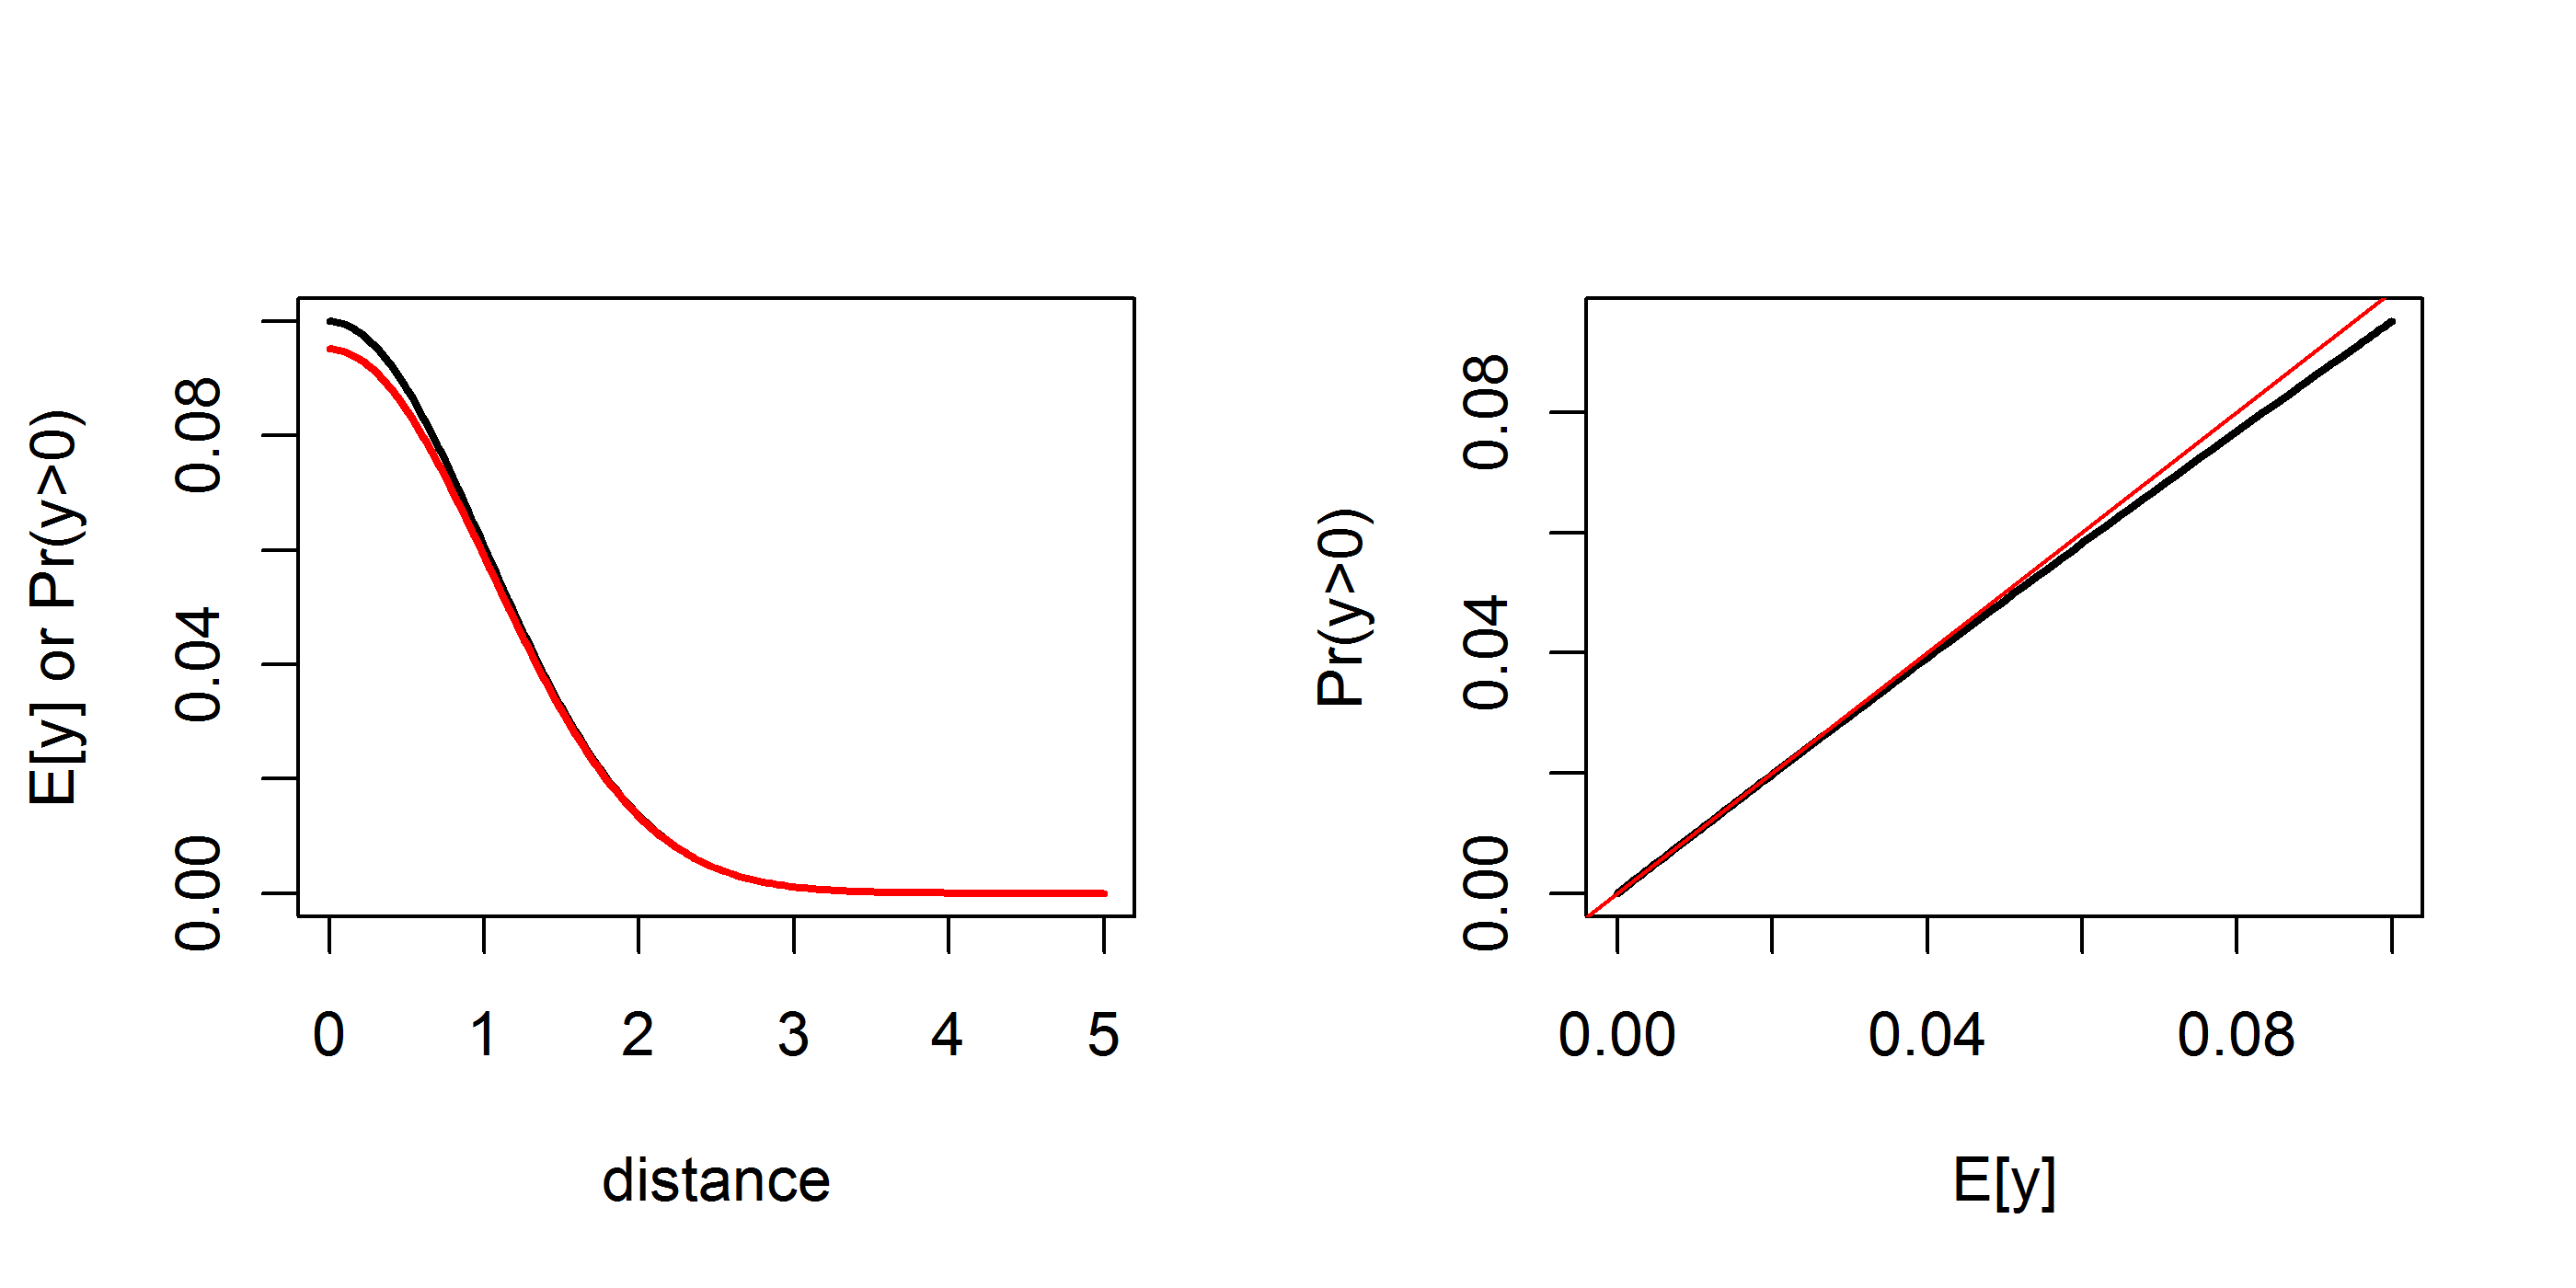
\includegraphics[width=5in,height=2.5in]{Ch9-PoisMn/figs/Poisson-Bern.png}
\caption{
Poisson approximation to the binomial. As the Poisson mean
approaches 0, then $\Pr(y>0)$ under the Poisson model approaches
$\lambda$ and therefore $y \sim \mbox{Poisson}(\lambda)$ is
well-approximated by a Bernoulli model with parameter $\lambda$.  }
\label{poisson-mn.fig.poissonbern}
\end{figure}

Even in such cases
where the Poisson and
Bernoulli models are
not quite
equivalent, we might choose to truncate
individual encounter frequencies to binary observations anyhow
(transforming counts to 0/1 is called ``quantizing'').  We might do
this intentionally in some cases, such as when the distinct encounter events are
highly dependent as often happens in camera trap studies when the same
individual moves back-and-forth in front of a camera during a short
period of time.
But sometimes,
truncation is a feature of the sampling. For example, in the case of
bear hair snares, the number of encounters might be well approximated
by a Poisson distribution but we cannot determine unique visits and so
only get to observe the binary event ``$y>0$''. Similarly for scat
sampling problems it will not generally be possible to diagnose
distinct ``independent'' scat samples. Under this model the data are
only binary encounters and we might therefore choose to model
encounter probability
using Eq. \ref{poisson-mn.eq.cloglog-inverse}.
Note that this is equivalent to using the complementary log-log link:
\[
\mbox{ cloglog}(p_{ij}) = \log(\lambda_{0})  + \log(k({\bf x},{\bf s}))
\]
where $\mbox{cloglog}(u) = \log(-\log(1-u))$.
\begin{comment}
This example shows us that the choice of link function is typically
directly related to a specific encounter frequency model and,
furthermore, the choice of link function is equivalent to choice of
``detection function.''
\end{comment}

\subsection{A cautionary note on modeling encounter frequencies}

Other models for counts might be appropriate. For example, ecologists
are especially fond of negative binomial models for count data
\citep{verhoef_boveng:2007,white_bennetts:1996,kery_etal:2005}
but other models for excess-Poisson variation are possible. For
example, we might add a normally distributed random effect to
the linear predictor \citep{coull_agresti:1999}.

As a general rule we favor the Bernoulli observation model even if
encounter frequencies are obtained by sampling.  The main reason is
that, with frequency data, we are forced to confront a model choice
problem (i.e., Poisson, negative binomial, log-normal mixture) that is
wholly unrelated to the fundamental space usage process that underlies
the genesis  % XXXX Again, Borchers might view this as too
             % narrow. i.e. it doesn't fit into his monkey counting
             % problem, or his frog counting using microphones
of many types of SCR data.
Repeated encounters over short time intervals
are not likely to be the result of independent encounter events. E.g.,
an individual moving back and forth in front of a camera yields a
cluster of observations that is not informative about the underlying
spatial structure of the population. Similarly in scat surveys dogs
are used to locate scats which are processed in the lab for
individuality \citep{kohn_etal:1999, mackay_etal:2008,
  thompson_etal:2012}.  The process of local scat deposition is not
strictly the outcome of movement or space usage but rather the outcome
of complex behavioral considerations as well as dependence in
detection of scat by dogs.
For example, dogs find (or smell) one scat and
then are more likely to find one or more nearby ones, if present, or
they get into a den or latrine area and find many scats.  The
additional assumption required to model variation in observed
frequencies (i.e., conditional on location) provides relatively no
information about space usage and density, and we feel that the model
selection issue should therefore be avoided.

To elaborate on this, we suppose that an individual with activity
center ${\bf s}$ visits a
particular pixel ${\bf x}$
% XXXX This notation might confuse people: "an individual s". ie, I think
% we have to be careful when we switch from s being an individual's
% activity center to s being an individual. Same goes for x being the
% location of a trap to x being a pixel.
with some probability $p({\bf x}, {\bf
  s})$, and then, once there, deposits a number of scat, or visits
a camera some number of times with frequency $y({\bf x},{\bf s}) \ge
0$.  We describe the outcome of this movement/usage process with a two-level
hierarchical model of the form: $[y|z][z|p({\bf x},{\bf s})]$ where
$z({\bf x},{\bf s})$ is a binary variable that indicates whether the
individual with activity center ${\bf s}$ used pixel ${\bf x}$
during some interval, and let $z({\bf x},{\bf s}) \sim
\mbox{Bernoulli}(p({\bf x},{\bf s}))$. If we suppose  encounter frequency
$y$ is independent of ${\bf x}$ and ${\bf s}$ conditional on the
use variable  $z$, then  we see that
the model for $y$ (amount of use) does not depend on ${\bf s}$.


\begin{comment}
Moreover, consideration of encounter frequency data could lead to
important identifiability problems along the lines of \citet{link:2003}. The
basic Poisson model can be over-dispersed in a number of ways to
produce different models of over-dispersion.  i.e., gamma noise,
normal noise, exponential noise, etc..  Thus we have different models
of heterogeneity, analogous to the class of models considered by
\citet{link:2003},
\end{comment}

\subsection{Analysis of the Poisson SCR model in BUGS}

We consider the simplest possible model here in which we have no
covariates that vary over sample occasions  $k=1,2,\ldots,K$
so that we work with
the aggregated individual- and trap-specific encounters:
\[
y_{ij} = (\sum_{k=1}^{K} y_{ijk}) =  \mbox{Poisson}(K  \lambda_{0}
k({\bf x}_{j},{\bf s}_{i}) )
\]
and we consider the bivariate normal form of $k({\bf x},{\bf s})$:
\[
k({\bf x},{\bf s}) = \exp( -d({\bf x}, {\bf
  s})^{2} /(2\sigma^{2}))
\]
so that
\[
\log( \lambda_{ij})  =\alpha_{0} + \alpha_{1} d({\bf x}_{j}, {\bf s}_{i})^2
\]
where $\alpha_{0} = \log(\lambda_{0})$ and $\alpha_1 = -1/(2\sigma^2)$.


As usual, we approach Bayesian analysis of these models using data
augmentation (Sec. \ref{closed.sec.da}).  Under data augmentation, we
introduce a collection of all-zero encounter histories to bring the
total size of the data set up to $M$, and a corresponding set of data
augmentation variables $z_{i} \sim \mbox{Bern}(\psi)$. Then the
observation model is specified conditional on $z$ according to:
\[
y_{ij} \sim  \mbox{Poisson}(z_{i} K  \lambda_{ij})
\]
% XXXX Do we want to call the augmented data "yz"?
which evaluates to a point mass at $y=0$ if $z=0$.  In other words,
the observation model under data augmentation is a zero-inflated
Poisson model which is easily analyzed by Bayesian methods, e.g., in
one of the {\bf BUGS} dialects or, alternatively, using likelihood
methods, which we neglect here although the same principles as in
Chapt. \ref{chapt.mle} apply.


\subsection{Simulating Data and Fitting the Model}


Simulating a sample SCR data set under the Poisson model requires only
a couple minor modifications to the procedure we used in
Chapt. \ref{chapt.scr0} (see the function \mbox{\tt simSCR0}). In
particular, we modify the block of code which defines the model to be
that of $\mathbb{E}(y)$ and not $\Pr(y=1)$, and we change the random
variable generator from \mbox{\tt rbinom} to \mbox{\tt rpois}:
\begin{samepage}
{\small
\begin{verbatim}
##
## S =activity centers and traplocs defined as in simSCR0()
##
D<- e2dist(S,traplocs) # Distance between activity centers and traps

## Define parameter values:
alpha0<- -2.5
sigma<- 0.5
alpha1<- 1/(2*sigma*sigma)

## Encounter probability model:
muy <-  exp(alpha0)*exp(-alpha1*D*D)

## Now generate the encounters of every individual in every trap
Y<-matrix(NA,nrow=N,ncol=ntraps)
for(i in 1:nrow(Y)){
 Y[i,]<-rpois(ntraps,K*muy[i,])
}
\end{verbatim}
}
\end{samepage}

We modified our simulation code from Chapt. \ref{chapt.scr0} to
simulate Poisson encounter frequencies for each trap and then we
analyze an ideal data set using {\bf BUGS}. This Poisson simulator
function {\tt simPoissonSCR} is available in the \mbox{\tt scrbook}
package (it can produce 3-d encounter history data too, although we
don't do that here).  Here is an example of simulating a data set and
harvesting the required data objects, and doing the data augmentation:

\begin{samepage}
{\small
\begin{verbatim}
data<-simPoissonSCR(discard0=TRUE,rnd=2013)
y<-data$Y
nind<-nrow(y)
X<-data$traplocs
K<-data$K
J<-nrow(X)
xlim<-data$xlim
ylim<-data$ylim

## Data augmentation
M<-200
y<-rbind(y,matrix(0,nrow=M-nind,ncol=ncol(y)))
z<-c(rep(1,nind),rep(0,M-nind))
\end{verbatim}
}
\end{samepage}

The process for fitting
the model in {\bf WinBUGS} or {\bf JAGS} is identical to what we've done
previously in Chapt. \ref{chapt.scr0}. In particular, we set up some
starting values, package the data and inits, identify the parameters
to be monitored, and then send everything off to our MCMC engine. Here
it all is for fitting the Poisson observation model (these commands
are shown in the help file for \mbox{\tt simPoissonSCR}):

{\small
\begin{verbatim}
sst<-X[sample(1:J,M,replace=TRUE),] # starting values for s
for(i in 1:nind){
if(sum(y[i,])==0) next
sst[i,1]<- mean( X[y[i,]>0,1] )
sst[i,2]<- mean( X[y[i,]>0,2] )
}
sst<-sst + runif(nrow(sst)*2,0,1)/8
data <- list (y=y,X=X,K=K,M=M,J=J,xlim=xlim,ylim=ylim)
inits <- function(){
  list (alpha0=rnorm(1,-2,.4),alpha1=runif(1,1,2),s=sst,z=z,psi=.5)
}
parameters <- c("alpha0","alpha1","N","D")

cat("
model {
alpha0~dnorm(0,.1)
alpha1~dnorm(0,.1)
psi~dunif(0,1)

for(i in 1:M){
 z[i] ~ dbern(psi)
 s[i,1]~dunif(xlim[1],xlim[2])
 s[i,2]~dunif(ylim[1],ylim[2])
for(j in 1:J){
d[i,j]<- pow(pow(s[i,1]-X[j,1],2) + pow(s[i,2]-X[j,2],2),0.5)
y[i,j] ~ dpois(lam[i,j])
lam[i,j]<- z[i]*K*exp(alpha0)*exp(- alpha1*d[i,j]*d[i,j])
}
}
N<-sum(z[])
D<- N/64
}
",file = "SCR-Poisson.txt")

library(R2WinBUGS)
out1 <- bugs (data, inits, parameters, "SCR-Poisson.txt", n.thin=1,n.chains=3,
 n.burnin=1000,n.iter=2000,working.dir=getwd(),debug=TRUE)
\end{verbatim}
}
{\flushleft Or, using {\bf JAGS} via \mbox{\tt rjags} we would do
  something like this:}
{\small
\begin{verbatim}
library(rjags)
jm <- jags.model("SCR-Poisson.txt", data=data, inits=inits, n.chains=3, n.adapt=1000)
out2 <- coda.samples(jm, parameters, n.iter=1000, thin=1)
\end{verbatim}
}
{\flushleft
Summarizing } the output from the {\bf WinBUGS}  run produces the following:
{\small
\begin{verbatim}
> print(out1,digits=2)
Inference for Bugs model at "SCR-Poisson.txt", fit using WinBUGS,
 3 chains, each with 2000 iterations (first 1000 discarded)
 n.sims = 3000 iterations saved
           mean    sd   2.5%    25%    50%    75%  97.5% Rhat n.eff
alpha0    -2.57  0.19  -2.95  -2.69  -2.57  -2.44  -2.19 1.00  2600
alpha1     2.34  0.36   1.69   2.08   2.32   2.57   3.12 1.00  3000
N        114.13 15.25  87.97 103.00 113.00 124.00 147.00 1.01   370
D          1.78  0.24   1.37   1.61   1.77   1.94   2.30 1.01   370
deviance 329.95 21.92 290.00 314.20 329.50 344.40 375.80 1.00  1700
...
[..some output deleted..]
...
\end{verbatim}
}

%We don't provide a real example of a Poisson SCR model here although
%we use this observation model for an analysis of some data in Chapt.
%\ref{chapt.searchencounter}. {\bf XXXX DO WE DO THIS ANYWHERE? XXXXX}


\subsection{Analysis of the Wolverine Study Data}

We reanalyzed the data from the wolverine camera trapping study that
were first introduced in Sec. \ref{scr0.sec.wolverine}.  We modified
the {\bf R} script from the function \mbox{\tt wolvSCR0} to fit the
Poisson model (see the help file for \mbox{\tt
  wolvSCR0pois}). Executing this function produces the results shown
in Tab. \ref{poisson-mn.tab.wolverine}.
\begin{table}
\centering
\caption{Results of fitting the SCR model with Poisson encounter
  frequencies to the wolverine camera trapping data.
Posterior summaries were obtained using {\bf WinBUGS} with
 3 chains, each with 6000 iterations, discarding the first 1000 as
 burn-in, to yield a total of 15000 posterior samples.
}
% XXXX Capitalize first letter of column headings?
\begin{tabular}{crrrrrrr} \hline \hline
 Parameter & mean &  sd & 2.5\% & 50\%  & 97.5\% &Rhat& n.eff \\ \hline
$\psi$     &  0.30& 0.07& 0.19 &  0.30 & 0.45& 1 &  650 \\
$\sigma$   &  0.64& 0.06& 0.54 &  0.64 & 0.76& 1 &  730 \\
$\lambda_{0}$& 0.06& 0.01& 0.04 &  0.06 & 0.08& 1&  5000\\
$\log(p_0)$  &-2.89& 0.17& -3.22& -2.89& -2.57& 1&  5000\\
$N$        & 60.12&11.91& 40.00& 59.00& 87.00& 1&   630\\
$D$        &  5.80& 1.15& 3.86 & 5.69 & 8.39 & 1&   630\\ \hline
%%%$\beta$  & 1.24& 0.21& 0.86 & 1.23 & 1.69 & 1&   730\\
\end{tabular}
\label{poisson-mn.tab.wolverine}
\end{table}
The results are almost indistinguishable from the Bernoulli model
fitted previously, where we had a posterior mean for $N$ of
 $59.84$,  $\sigma$ it was
$0.64$. The {\bf R}
script is provided in the  \mbox{\tt scrbook} package which you can
use to modify the model or obtain more posterior samples.
%In addition we did a basic assessment of Goodness-of-fit using a
%Bayesian p-value and statistic 1 as described in sec. XXXXX.

\subsection{Count detector models in the  \mbox{\tt secr} package}

The {\bf R} package \mbox{\tt secr} will fit Poisson or negative
binomial encounter frequency models. The formatting of data and
structure of the analysis proceeds in a similar fashion to the
Bernoulli model described in Sec. \ref{mle.sec.secr}, except that
we specify the \mbox{\tt detector=``count''} option when the traps
object is created. The set-up proceeds as follows:
\begin{samepage}
{\small
\begin{verbatim}
library(secr)
library(scrbook)
data(wolverine)

traps<-as.matrix(wolverine$wtraps)
dimnames(traps)<-list(NULL,c("trapID","x","y",paste("day",1:165,sep="")))
traps1<-as.data.frame(traps[,1:3])
trapfile1<-read.traps(data=traps1,detector="count")
\end{verbatim}
}
\end{samepage}
You can proceed with analysis of these data and compare/contrast with
the Bayesian analysis given above, or the results of the Bernoulli
model fitted in Chapt. \ref{chapt.mle}.



\section{Independent Multinomial Observations}
\label{poisson-mn.sec.multinomial}

Several types of encounter devices yield multinomial observations in
which an individual can be caught in a single trap during a particular
encounter occasion, but traps might catch any number of individuals.
Mist netting is the canonical example of such a ``multi-catch'' traps
\citep{efford_etal:2009euring}. Also some kinds of bird or mammal
cage-traps hold multiple animals, as do pit-fall traps which are
commonly used for many types of herptiles.  Another type of sample
method that might be viewed (in some cases) as a multi-catch device
are area-searches of, for example, reptiles where we think of a small
polygon as the ``trap'' -- we could get multiple individuals (turtles,
lizards) in the same plot but not, in the same sample occasion, at
different plots.  The key features of this model are: (1) capture of
an individual in a trap is {\it not} independent of its capture in
other traps, because initial capture precludes capture in any other
trap and (2) individuals behave independently of one another, so
whether a trap captures some individual doesn't have an affect on
whether it captures another.  A type of model in which the 2nd
assumption is violated are the ``single catch'' trap systems which we
address in Sec. \ref{poisson-mn.sec.singlecatch} below. In general we
could imagine non-independence being important in any multi-catch
situation but to the best of our knowledge a general model that
encompasses complete dependence (i.e., single-catch) and complete
independence (multi-catch) of individuals has not been proposed.  So
we treat the cases individually and, in this section, we address the
multi-catch situation wherein individuals behave independently.


In this case we assume the observation ${\bf y}_{ik}$ for individual
$i$ during sample occasion $k$ is a multinomial observation which
consists of a sequence of 0's and  a single 1 indicating the
trap of capture, or ``not captured''. For the ``not captured'' event
we define an additional outcome, by convention element $J+1$ of the
vector.  As an example, if we capture an individual in trap 2 during
some occasion of a
6 sample period study then the multinomial observation has length $J+1
= 7$, and the observation is ${\bf y}_{i} = (0,1,0,0,0,0,0)$. An
individual not captured at all would have the observation vector
$(0,0,0,0,0,0,1)$.  If we sample for 5 occasions
in all and the
individual is also caught in trap 4 during occasion 3, but otherwise
uncaptured, then the 5 encounter observations for that individual are
as follows:
% XXXX Suggest emphasizing (again) that column 7 is not a trap, but
% indicates "not captured"
\begin{verbatim}
occassion  |-------trap -------| "not captured"
           1   2   3   4   5   6      7
           ------------------------------------
   1       0   1   0   0   0   0      0
   2       0   0   0   0   0   0      1
   3       0   0   0   1   0   0      0
   4       0   0   0   0   0   0      1
   5       0   0   0   0   0   0      1
\end{verbatim}
Statistically we regard the {\it rows} of this data matrix as {\it
  independent} multinomial trials.

Analogous to our previous Bernoulli and Poisson models, we seek to
construct the multinomial cell probabilities for each individual, as a
function of {\it where} that individual lives, through its center of
activity ${\bf s}$. Thus we suppose that
\begin{equation}
 {\bf y}_{ik}|{\bf s}_{i} \sim \mbox{Multinom}(1, {\bm \pi}({\bf s}_{i}) )
\label{poisson-mn.eq.mn}
\end{equation}
where ${\bm \pi}({\bf s}_{i})$ is a vector of length $J+1$, where
$\pi_{i,J+1}$, the last cell, corresponds to the probability of the
event ``not captured''.  Now we have to construct these cell
probabilities in some meaningful way that depends on each individual's
${\bf s}$.  We use the standard multinomial logit with distance as a
covariate:
\[
 \pi_{ij} = \frac{  \exp(\alpha_{0} + \alpha_{1} d_{ij}) }{ 1+ \sum_{j}
   \exp(\alpha_{0} + \alpha_{1} d_{ij})}
\]
for $j=1,2,\ldots,J$ and, for $J+1$, i.e., ``not captured'',
\[
 \pi_{i,(J+1)} = \frac{  \exp(0) }
                    { 1+ \sum_{j} \exp(\alpha_{0} + \alpha_{1} d_{ij})}
\]
or, more commonly, we use $d_{ij}^{2}$ to correspond to our Gaussian
kernel model for encounter probability. Whatever function of distance
we use in the construction of multinomial probabilities will have a
direct correspondence to the standard encounter probability models we
used in the Bernoulli or Poisson models as well (see
Sec. \ref{scr0.sec.implied}).

It is convenient to express these multinomial models short-hand as
follows, e.g., for the Gaussian encounter probability model:
\[
\mbox{mlogit}( \pi_{ij} ) = \alpha_{0} + \alpha_{1} d_{ij}^{2}
\]
In this way we can refer to models with covariates in a more concise
way. For example, a model with a trap-specific covariate, say $C_{j}$, is:
\[
\mbox{mlogit}( \pi_{ij} ) = \alpha_{0} + \alpha_{1} d_{ij}^{2} + \alpha_{2} C_{j}
\]
or we could include occasion-specific covariates too, such as
behavioral response.

A statistically equivalent distribution to the multinomial is the {\it
  categorical} distribution.  If ${\bf y}$ is a multinomial trial with
probabilities ${\bm \pi}$ than the {\it position} of the non-zero
element of ${\bf y}$ is a categorical random variable with
probabilities ${\bm \pi}$.  We express this for SCR models as
\[
{\bf y}|{\bf s} \sim \mbox{Categorical}( {\bm \pi}({\bf s})) )
\]
In the SCR context, the categorical version of the multinomial trial
corresponds to the {\it trap of capture}.  Using our example above
with 6 traps then we could as well say $y_{ik}$ is a categorical
random variable with possible outcomes $(1,2,3,4,5,6,7)$ where outcome
$y=7$ corresponds to ``not captured.'' Obviously, how this is
organized or labeled is completely irrelevant, although it is
convenient to use the integers $1$ to $(J+1)$ where $J+1$ is the event
not captured.  Therefore, for our illustration in the previous table,
$y_{i1} = 2$, $y_{i2} = 7$, $y_{i3} = 4$ and so on.

For simulating and fitting data in the {\bf BUGS} engines we will
typically use the categorical representation of the model because it
is somewhat more convenient.  We have found that fitting multinomial
models in {\bf WinBUGS} is less efficient than {\bf JAGS}
\citep{royle_converse:2013}, which we use in the subsequent examples
involving multinomial observation models.


\subsection{Multinomial  Resource Selection Models}

The multinomial probabilities in Eq. \ref{poisson-mn.eq.mnprobs}
look similar to the
multinomial resource selection function (RSF) model for telemetry data
\citep{manly_etal:2002, lele_keim:2006}.  This suggests how we might
model landscape or habitat covariates using such methods -- i.e., by
including them as explicit covariates in a larger multinomial model
for ``use'' -- which, if we take the product of use with encounter
produces a model for the observable encounter data. This
leads naturally to the development of models that integrate RSF data
from telemetry studies with SCR data
\citep{royle_etal:2012mee},
which is the topic of  Chapt. \ref{chapt.rsf}.



\subsection{Simulating data and analysis using JAGS}

We're going to show the nugget of a simulation function which is
used in the function \mbox{\tt simMnSCR} found in the {\bf R} package
\mbox{\tt scrbook}.  The first lines of the following {\bf R} code
make use of some things that you need to define, but we omit them here
(e.g., \mbox{\tt xlim}, \mbox{\tt ylim} are the boundaries of the
state-space, \mbox{\tt N} is the population size, etc..):
% XXXX Okay, but briefly explain Xl, Xu, ...
\begin{samepage}
{\small
\begin{verbatim}
##
## Simulate random activity centers:
## (first define N, xlim, ylim, etc..)
##
S<-cbind(runif(N,xlim[1],xlim[2]),runif(N,ylim[1],ylim[2]))

## Distance from each individual to each trap
D<- e2dist(S,traplocs)

## Set paramter values
sigma<- 0.5
alpha0<- -1
alpha1<- -1/(2*sigma*sigma)

## make an empty data matrix and fill it up with data
Ycat<-matrix(NA,nrow=N,ncol=K)
for(i in 1:N){
  for(k in 1:K){
    lp<- alpha0 + alpha1*D[i,]*D[i,]
    cp<- exp(c(lp,0))
    cp<- cp/sum(cp)
    Ycat[i,k]<- sample(1:(ntraps+1),1,prob=cp)
  }
}
\end{verbatim}
}
\end{samepage}
The resulting data matrix in this case has the maximal dimension $N$
and so, for analysis, to mimic a real situation, we would have to
discard the uncaptured individuals.  The function \mbox{\tt
  simMnSCR} in the package \mbox{\tt scrbook} will also simulate
data that includes a behavioral response
%(the parameter
%labeled \mbox{\tt alpha2} shown in the {\bf R} code below),
 which will be the
typical situation in small-mammal trapping problems
\citep[see][for details]{converse_royle:2012}.

Here we use our function \mbox{\tt simMnSCR} to simulate a data set
with $K=7$ occasions.
We'll run the model using \mbox{\tt JAGS}
which we have found is much more effective for this class of models.
We get the data set-up for analysis by augmenting the size of the data
set to $M=200$. In addition we choose starting values for ${\bf s}$
and the data augmentation variables $z$.  For starting values of ${\bf
  s}$ we cheat a little bit here and use the true values for the
observed individuals and then augment the $M \times 2$ matrix ${\bf
  S}$ with $M-n$ randomly selected activity centers. Our function
\mbox{\tt spiderplot} returns the mean observed location of
individuals for use as starting values.  The parameters input to
\mbox{\tt simMnSCR} are the intercept $\alpha_{0}$, $\sigma =
\sqrt{1/(2\alpha_{1})}$ for the Gaussian encounter probability model,
and $\alpha_{2}$ is the behavioral response parameter. The data
simulation and set-up proceeds as follows:
\begin{samepage}
{\small
\begin{verbatim}
set.seed(2013)
parms<-list(N=100,alpha0= -.40, sigma=0.5, alpha2= 0)
data<-simMnSCR(parms,K=7,ssbuff=2)
nind<-nrow(data$Ycat)

M<-200
Ycat<-rbind(data$Ycat,matrix(nrow(data$X)+1,nrow=(M-nind),ncol=data$K))
Sst <-rbind(data$S,cbind(runif(M-nind,data$xlim[1],data$xlim[2]),
                         runif(M-nind,data$ylim[1],data$ylim[2])))
zst<-c(rep(1,160),rep(0,40))
\end{verbatim}
}
\end{samepage}

The model specification is not much more complicated than the binomial
or Poisson models given previously. The main consideration is that we
define the cell probabilities for each trap $j=1,2,\dots,J$ and then
define the last cell probability, $J+1$, for ``not captured'', to be
the complement of the sum of the others. The code is shown in Panel
\ref{poisson-mn.panel.mn}.  In the last lines of code here we specify
$N$ and density, $D$, as derived parameters.

% XXXX Sometimes you use "xlim" and sometimes "Xl" and "Xu". Okay,
% people shouldn't be idiots but there we need to simplify the sea of notation
%% ANDY: RIGHT -- TRYING TO USE/(convert to) "xlim" "ylim" throughout.
\begin{panel}[htp]
\centering
\rule[0.15in]{\textwidth}{.03in}
{\small
\begin{verbatim}
cat("
model {
psi ~ dunif(0,1)
alpha0 ~ dnorm(0,10)
sigma ~dunif(0,10)
alpha1<-  -1/(2*sigma*sigma)

for(i in 1:M){
  z[i] ~ dbern(psi)
  S[i,1] ~ dunif(xlim[1],xlim[2])
  S[i,2] ~ dunif(ylim[1],ylim[2])
  for(j in 1:ntraps){
    #distance from capture to the center of the home range
    d[i,j] <- pow(pow(S[i,1]-X[j,1],2) + pow(S[i,2]-X[j,2],2),1)
  }
  for(k in 1:K){
    for(j in 1:ntraps){
      lp[i,k,j] <- exp(alpha0 + alpha1*d[i,j])*z[i]
      cp[i,k,j] <- lp[i,k,j]/(1+sum(lp[i,k,]))
    }
    cp[i,k,ntraps+1] <- 1-sum(cp[i,k,1:ntraps])  # last cell = not captured
    Ycat[i,k] ~ dcat(cp[i,k,])
  }
}

N <- sum(z[1:M])
A <- ((xlim[2]-xlim[1])*trap.space)*((ylim[2]-ylim[1])*trap.space)
D <- N/A
}
",file="model.txt")

\end{verbatim}
}
\rule[-0.15in]{\textwidth}{.03in}
\caption{
{\bf BUGS} model specification for the independent multinomial
observation model. For data simulation and model fitting see the
help file \mbox{\tt ?simMnSCR} in the {\bf R} package \mbox{\tt scrbook}.
}
\label{poisson-mn.panel.mn}
\end{panel}

To fit the model, we need to package everything up (inits, parameters,
data) and send it off to \mbox{\bf JAGS} to build an MCMC simulator
for us (these commands are executed in the help file for \mbox{\tt
  simMnSCR}). In addition to the usual data objects, we also pass
the limits of the assumed rectangular state-space (\mbox{\tt ylim},
\mbox{\tt xlim}, both $1 \times 2$ vectors) and the scale of the
standardized units, called \mbox{\tt trap.space} here because we
typically will define the trap coordinates to be an integer grid. If
the trap spacing is 10 $m$ and we want units of density computed in
terms of individuals {\it per} meter, then we input \mbox{\tt
  trap.space=10}. The analysis is carried out as follows:
\begin{samepage}
{\small
\begin{verbatim}
inits <- function(){  list (z=zst,sigma=runif(1,.5,1) ,S=Sst) }

# parameters to monitor
parameters <- c("psi","alpha0","alpha1","sigma","N","D")

# bundle the data. Note this reuses "data"
data <- list (X=data$X,K=data$K, trap.space=1,Ycat=Ycat,M=M,
        ntraps=nrow(data$X),ylim=data$ylim,xlim=data$xlim)

library(R2jags)
out <- jags (data, inits, parameters, "model.txt", n.thin=1,
        n.chains=3, n.burnin=1000, n.iter=2000)
\end{verbatim}
}
\end{samepage}

The posterior summaries are provided in the following {\bf R}
output (recall that
$N=100$, $\alpha_{0}= -.40$, and $\sigma=0.5$):
{\small
\begin{verbatim}
Inference for Bugs model at "model.txt", fit using jags,
 3 chains, each with 2000 iterations (first 1000 discarded)
 n.sims = 3000 iterations saved
         mu.vect sd.vect    2.5%     25%     50%     75%   97.5%  Rhat n.eff
D          1.873   0.189   1.531   1.750   1.859   2.000   2.250 1.006  1300
N        119.867  12.107  98.000 112.000 119.000 128.000 144.000 1.006  1300
alpha0    -0.435   0.151  -0.738  -0.535  -0.439  -0.331  -0.146 1.004   580
alpha1    -2.195   0.286  -2.785  -2.372  -2.180  -2.004  -1.658 1.003  2800
psi        0.599   0.069   0.465   0.552   0.599   0.645   0.739 1.006  1400
sigma      0.480   0.032   0.424   0.459   0.479   0.500   0.549 1.003  2400
deviance 892.164  21.988 850.922 877.417 891.561 906.246 937.728 1.003   950

[... output deleted ....]
\end{verbatim}
}


\subsection{Multinomial Relationship to Poisson}

The multinomial is related to the Poisson encounter rate
model by a conditioning argument. Let $y_{ij}$ be the number of
encounters for individual $i$ in trap $j$. If $y_{ij} \sim
\mbox{Poisson}(\lambda_{ij})$,
then,
conditional on the {\it total}
number of captures (i.e., across all traps), $y_{i} = \sum_{j}
y_{ij}$, the trap encounter frequencies are multinomial with
probabilities
\[
 \pi_{ij} =  \frac{ \lambda_{ij} } { \sum_{j} \lambda_{ij} }
\]
for $j=1,2,\ldots,J$.
Or equivalently the {\it trap of
  capture} is categorical with probabilities $\pi_{ij}$ as given above.
Under the Gaussian kernel model, these probabilities are:
\begin{equation}
\pi_{ij} =  \frac{ \exp(  \alpha_{1}  d({\bf x}_{i},{\bf s}_{i})^2 ) }  {
   \sum_{j} \exp( \alpha_{1} d({\bf x}_{i},{\bf s}_{i})^2)}
\label{poisson-mn.eq.mnprobs}
\end{equation}
where, we note, the intercept $\alpha_{0}$ has canceled from both the
numerator and denominator. This makes sense because, here, these
probabilities describe the trap-specific capture probabilities {\it
  conditional on capture}.  Therefore, the model is not completely
specified, absent a model for the ``overall'' probability of encounter
or the expected frequency of captures, say $\phi_{i}$. Depending on
how we specify a model for this quantity $\phi_{i}$, we can reconcile
it directly with the Poisson model.
% or the Bernoulli model of
%Chapt. \ref{chapt.scr0}.
Let $y_{i.}$ be the total number of encounters for individual $i$ and
suppose $y_{i.}$ has a Poisson distribution with mean $\phi_{i}$.
Then, marginalizing Eq. \ref{poisson-mn.eq.mn} over the Poisson
distribution for $y_{i.}$ produces the original set of
$iid$ % XXXX I have been using "i.i.d." Should I change to $iid$?
Poisson
frequencies with probabilities:
\[
 \lambda_{ij} = \phi_{i} \pi_{ij}
\]
for $j=1,2,\ldots,J$.
In particular, if we suppose that
$\phi_{i} = \sum_{j} \exp(\alpha_{0} + \alpha_{1} d({\bf x},{\bf s})^2)$
then the marginal distribution of $y_{ij}$ is Poisson with mean $\exp(
\alpha_{0} + \alpha_{1} d({\bf x},{\bf s})^2 )$, equivalent to
Eq. \ref{poisson-mn.eq.lp}.
%An alternative choice of $\phi_{i}$ under the assumption that $y_{i}$ is
%binomial will produce individual- and trap-specific probabilities
%consistent with the binomial model SCR0.
\begin{comment}
  Suppose, instead, that $y_{i}$ is Binomial with sample size $K$ and
  probability $\phi_{i}$. How should we parameterize $\phi_{i}$?  One
  possibility is
\[
\phi_{i} = \lambda_{0} \exp(-\alpha_{1} \sum_{j} d_{ij}^2)
\]
%this is not unnatural we can think of hazard to capture in each trap
%as independent and then sum up the hazards and this is (the
%complement) of the ``mortality function''.
\end{comment}

In summary, the Poisson and multinomial models are equivalent in how
they model the distribution of captures among traps.
 It stands to reason that, if the encounter
rate of individuals is low, we could use the Poisson and multinomial
models interchangeably. In fact, based on our discussion in Sec.
\ref{poisson-mn.sec.approx}
above we could use any of the binomial/Poisson/multinomial models with
little ill-effect when encounter rate is low.



%So we can think of this multinomial model as arising naturally
%by having Poiosson encounters and then conditioning on the total.
%It is a sensible model to have anyhow, as it just allocates captures
%to traps in proportion to the square of distance.  We could try other
%models here too (Note: What do Borchers and Efford 2008 do?).

%People might think this multinomioal model is somehow more general
%than assuming Poisson encounter frequencies since we might cook up the
%multinomioal without having to specify a distribution for
%$y_{i}$. That said, we note that it arises under
%If we now uncondition on the total.....
%$y_{ij}$ is Poisson with mean $\sum_{j}$ stuff... we have a product of
%Poissons, i.e., the model we started with.

\begin{comment}
The interpretation of this formulation of the multinomial model merits
some discussion. That is, {\it given that an individual is captured},
the probabilities given by Eq. \ref{poisson-mn.eq.mnprobs} determine
the probability distribution of ``trap of capture''.  The probability
that individual $i$ is captured in trap $j$ is the product of two
components
\[
\pi_{ij} = \Pr(\mbox{individual} i \mbox{captured in trap} j) =
 \Pr(\mbox{captured in trap} j | \mbox{captured at all})\Pr(\mbox{captured at all})
\]
To fully specify the model, we have to model the probability that an
individual is captured at all, say $p_0$. Then the unconditional
multinomial probabilities are $p_{0} \pi_{ij}$ for $j=1,\ldots,J$ and
$\pi_{i,J+1} = (1-p_{0})$.  It hardly makes sense that $p_{0}$ should
be constant.  Instead, it is natural to think that total probability
of capture should be related to the average distance to traps like
this:
\[
 p_{i} = p_{0} \exp(-\beta \sum_{j} D_{ij}^2)
\]
the argument to justify this is that the total hazard to capture, if
traps function independently, is the sum of that due to each trap, i.e.,
\[
 h_{i} = \sum_{j} h_{ij}
\]
so we set $h_{ij} = \propto D_{ij}^{2}$ which I think is the Gompertz
hazard model.
%Then
%the the survival function $S=exp(-H)$ so we equate $p$ to ``survival'' (hardly makes sense
%but, hey, thats the model that people use).
Then we have the marginal probability of capture in trap $j$ is
(multiplying $p_{i}$ with $\pi_{ij}$):
\[
\pi_{ij} =   p_{0}  \exp(-\beta D_{ij}^2)
\]
and then the probability of not being captured at all is
\[
 \pi_{i,J+1} =  1-p_i
\]
Therefore the multinomial trial ${\bf y}_{i}$ of length  $(J+1)
XXXX problem here -- do those add up to 1? XXXXX
XXX
\times 1$ has those probabilities.  One issue: This induces a
constraint on $p_{0}$ because the sum of the multinomial probabilities
has to be 1 and therefore
\[
p_{0} \sum_{j} p_{ij} \le 1.
\]
References to Royle et al. 2009a and Gardner et al. 2010 need to go
here because those papers used this type of model. (misspecified
multinomial).
This is not the ``multivariate logit'' that
we use in the BUGS model above which more naturally admits the
restriction on the cell probabilities, see Eq. XXXX above.


In summary, there is a coherent linkage between the Poisson,
multinomial, and the Binomial model. If trap-level encounter
histories are $iid$ Poisson random variables with $\lambda_{ij} =
\lambda_{0}exp(-\alpha_{1} d^{2})$, then the trap-of-capture,
conditional on the total number of captures, has a multinomial
distribution with cell probabilities $\pi_{ij} =
\lambda_{ij}/(\sum_{j} \lambda_{ij})$ and then if the hazard to
capture is proportion to $d^{2}$, and the traps are independent, then
$\pi_{ij} = p_{0} exp(-\alpha_{1} d_{ij}^{2})$ with a restriction on
$p_{0}$.  So those models are all
equivalent to some extent, for their appropriate observation model.

\end{comment}



\section{Avian Mist-Netting Example}
\label{poisson-mn.sec.ovenbird}

We analyze data from a mist-netting study of ovenbirds, conducted
at the
Patuxent Wildlife Research Center, Laurel MD, by DK Dawson and MG
Efford. The data from this study are available in the \mbox{\tt secr}
package, and have been analyzed previously by
\citet{efford_etal:2004}, see also \citet{borchers_efford:2008}.
Forty-four mist nets spaced 30 m apart on the perimeter of a 600-m x
100-m rectangle
were operated on 9 or 10 non-consecutive
days in late May and June for 5 years from 2005-2009.  From the
\mbox{\tt secr} documentation of this data set we take this:
\begin{quote}
{\it
  Netting was passive (i.e. song playback was not used to lure birds
  into the nets). Birds received individually numbered bands, and both
  newly banded and previously banded birds were released at the net
  where captured. Sex was determined in the hand from the presence of
  a brood patch (females) or cloacal protuberance (males).}
\end{quote}
The ovenbird
data can be loaded as follows:
\begin{verbatim}
library(secr)
data(ovenbird)
\end{verbatim}
The dataset consists of adult ovenbirds caught during sampling in each
of 5 years, 2005-2009. (one ovenbird was killed in 2009, indicated by
a negative net number in the encounter data file)\index{loss-on-capture}.
As with most mist-netting studies, nets are checked multiple times
during a day (e.g., every hour during a morning session). However, for
this data set, the within-day recaptures are not included so each bird
has at most a single capture per day. Therefore the multinomial model
(detector type `multi' in \mbox{\tt secr}) is appropriate.
 Although
several individuals were captured in more than one year, this
information is not used in the models presently offered in \mbox{\tt
  secr}, but we do make use of it in the development of open models in
Chapt. \ref{chapt.open}.
%
%{\it
%  An analysis of the data for males in the first four years showed
%  that they tended to avoid nets after their first capture within a
%  season (Dawson and Efford 2009). While the species was present
%  consistently, the number of detections in any one year was too small
%  to give reliable estimates of density; pooling of detection
%  parameters across years helped to improve precision.
%}


\subsection{Multiple Sample Sessions}

Up to this point we have only dealt with a basic closed population
sampling situation consisting of repeated sample occasions of a single
population of individuals using a single array of traps. In practice,
many studies produce repeated samples over time, or at different
locations -- we adopt the \mbox{\tt secr} terminology of {\it session}
for such replication by groups of time or space, and the models are
{\it multi-session} models, although we think of such models as being
relevant to any stratified population (see Chapt. \ref{chapt.hscr}).
We introduced \mbox{\tt secr}'s
multi-session models in Sec. \ref{mle.sec.multisession}.  In the case
of the ovenbird data, sampling was carried out in multiple years, with
a number of sample occasions within each year (9 or 10), a type of
data structure commonly referred to as ``the robust
design''\index{robust design} \citep{pollock:1982}.  In this context,
it stands to reason that there is recruitment and mortality happening
across years. In Chapt. \ref{chapt.open} we model these processes
explicitly but, here, we provide an analysis of the data that does not
require explicit models for recruitment and survival, regarding the
yearly populations as independent strata, and fitting a multi-session
model.

What exactly is the multi-session model that \mbox{\tt secr} fits? The
model can be thought of as a type of open population model, either
with explicit time periods that represent sessions, or by equating
spatial units to sessions.  A special case of open models arises when
we assume $N_{t}$ (time-specific population sizes) are independent
from one time period or session to the next -- this can be thought of
as a ``random temporary emigration'' model of the
\citet{kendall_etal:1997} variety, and this is essentially the
multi-session model implemented in \mbox{\tt secr}.  In particular, by
assuming that $N_{t}$ is Poisson with mean $\Lambda_{t}$ one can model
variation in abundance among sessions based on the Poisson-integrated
likelihood in which parameters of $\Lambda_{t}$ appear directly in the
likelihood as we noted in Sec. \ref{mle.sec.multisession}.  We provide
an analysis (below) of the ovenbird data here using the multi-session
models in \mbox{\tt secr}.  We formalize the multi-session model
approach from a Bayesian perspective using data augmentation in
Chapt. \ref{chapt.hscr}, based on \citet{converse_royle:2012} and
\citet{royle_converse:2013}.

A 3rd way to develop multi-session models which is convenient for {\bf
  BUGS} is to regard the data from each session as an independent data
set with its own $N_{t}$ parameter, and do $T$ distinct data augmentations. Because each $N_{t}$ is regarded
as a free parameter, independent of the other parameters, we'll call
this the nonparametric multi-session model.
We can analyze this model
in the normal context of data augmentation by augmenting each year
separately in the same {\bf BUGS} model specification. This approach
avoids making explicit model assumptions about the $N_{t}$
parameters.  This is distinct from the model implemented in \mbox{\tt
  secr} in that \mbox{\tt secr} is removing the $N_{t}$ parameters by
integrating the conditional-on-$N_{t}$ likelihood over the Poisson
prior for $N_{t}$.
% XXXX Are you sure that this is what secr is doing? Where is the
% documentation explaining how secr fits multi-session models? They
% never actually sum over all possible values of N, right?

We
demonstrate all of the 3 approaches with the ovenbird data: In the
following section we provide the nonparametric model with
unconstrained $N_{t}$,
 and we demonstrate  the model-based
multi-session models from \mbox{\tt secr} both here (following section) and in
Chapt. \ref{chapt.hscr} from a Bayesian standpoint.
We address the fully open ``Spatial Jolly-Seber''
model in Chapt. \ref{chapt.open},


\subsection{Analysis in JAGS}

The ovenbird data are provided as a multi-session \mbox{\tt capthist}
object \mbox{\tt ovenCH} which, by regarding years as independent
strata, allows for the fitting of the multi-session model.  For doing
a Bayesian analysis in one of the {\bf BUGS} engines (we use {\bf
  JAGS} here) there are a number of ways to structure the data and
describe the model.  We can analyze either a 2-d data set with all
years (data augmented) ``stacked'' into a data set of dimension $(5*M)
\times 10$ (5 years, $M=$ size of the augmented data set, $K=10$
replicate sample occasions). Or, we could produce a 3-d array ($M \times J
\times K$). We adopted the former approach, analyzing the data as a
2-d array and creating an additional indicator variable for ``year''
to indicate which stratum (year) each record goes with.  There was a
single loss-on-capture which we accounted for by fixing $p=0$ for all
subsequent encounters of that individual (indicated by the binary
variable \mbox{\tt dead}, as shown in Panel
\ref{poisson-mn.panel.ovenbird}).  We have an {\bf R} script in
\mbox{\tt scrbook} package called \mbox{\tt SCRovenbird}, so you can
see how to set-up the data and run the model.  Executing the script
\mbox{\tt SCRovenbird} produces the posterior summaries given in Table
\ref{scrovenbird.results}. Here, density is in units of birds per ha.


Data on individual sex is included
with \mbox{\tt secr}, but  we provide an analysis of a single model
for all adults, constant $\sigma$ across years, constant $p_{0}$, and
year-specific values of $N_{t}$ (and hence $D_{t}$).
 There is a habitat mask provided with the data but the mask
appears to just be a modified rectangle around the net locations,
clipped to have rounded corners, and so we don't use it here.






\begin{panel}[htp]
\centering
\rule[0.15in]{\textwidth}{.03in}
%\begin{minipage}{2.5in}
{\small
\begin{verbatim}
model {
 alpha0 ~ dnorm(0,.1)
 sigma ~dunif(0,200)
 alpha1<- 1/(2*sigma*sigma)

 A <- ((xlim[2]-xlim[1]))*((ylim[2]-ylim[1]))
 for(t in 1:5){
  N[t] <- inprod(z[1:bigM],yrdummy[,t])
  D[t] <- (N[t]/A)*10000  # put in units of per ha
  psi[t] ~ dunif(0,1)
 }
# bigM = total size of jointly augmented data set
 for(i in 1:bigM){
   z[i] ~ dbern(psi[year[i]])
   S[i,1] ~ dunif(xlim[1],xlim[2])
   S[i,2] ~ dunif(ylim[1],ylim[2])
# X = trap locations, S = activity centers
 for(j in 1:ntraps){
    d2[i,j] <- pow(pow(S[i,1]-X[j,1],2) + pow(S[i,2]-X[j,2],2),1)
  }
 for(k in 1:K){
   Ycat[i,k] ~ dcat(cp[i,k,])
   for(j in 1:ntraps){
     lp[i,k,j] <- exp(alpha0 - alpha1*d2[i,j])*z[i]*(1-dead[i,k])
     cp[i,k,j] <- lp[i,k,j]/(1+sum(lp[i,k,1:ntraps]))
   }
   cp[i,k,ntraps+1] <- 1-sum(cp[i,k,1:ntraps])  # last cell = not captured
 } }  }
\end{verbatim}
}
%\end{minipage}
\rule[-0.15in]{\textwidth}{.03in}
\caption{
{\bf BUGS} model specification for the non-parametric multi-session
model in which each $N_{t}$ is independent of the other. The implied
prior (by data augmentation) is that $N_{t} \sim
\mbox{Uniform}(0,100)$.
To fit this model to the ovenbird data, see
 \mbox{\tt ?SCRovenbird} in the {\bf R} package \mbox{\tt scrbook}.
}
\label{poisson-mn.panel.ovenbird}
\end{panel}


\begin{table}[t!]
\centering
  \small
  \caption{Inference for the ovenbird mist-netting data using the
    independent multinomial observation model. MCMC was done using
    {\tt jags} with 3 chains, each with 5000 iterations, discarding
    the first 1000, for a total of 12000 posterior samples.}
  \begin{tabular}[t]{crrrrrrr}
    \hline \hline
parameter   &  mu.vect &  sd.vect &  2.5\%  &  50\%  &  97.5\%  & Rhat &  n.eff \\
    \hline
D[1] &   1.056  &  0.177 &  0.778 &  1.037 &  1.469 &  1.001 & 12000 \\
D[2] &    1.109 &  0.174 &  0.835 &  1.095 &  1.498 &  1.002 &  1600 \\
D[3] &    1.302 &  0.187 &  0.979 &  1.296 &  1.728 &  1.002 &  2700 \\
D[4] &    0.959 &  0.159 &  0.691 &  0.951 &  1.296 &  1.001 &  8000 \\
D[5] &    0.811 &  0.146 &  0.576 &  0.807 &  1.152 & 1.002  &  2000 \\
N[1] &   36.666 &  6.132 &  27.000 &  36.000 &  51.000 &  1.001 &  12000 \\
N[2] &   38.513 &  6.056 & 29.000  &  38.000 &  52.000 & 1.002 &  1600 \\
N[3] &   45.197 &  6.501 & 34.000 &  45.000  &  60.000 &  1.002 & 2700 \\
N[4] &   33.279 &  5.511 & 24.000 &  33.000  &  45.000 &  1.001 &  8000 \\
N[5] &   28.145 &  5.071 &  20.000 &  28.000 &  40.000 &  1.002 &  2000 \\
alpha0 &  -3.528 &   0.164 & -3.853 &  -3.530 &  -3.208 &  1.002 &  1700 \\
alpha1 &  0.000 &  0.000 &  0.000 &  0.000 &  0.000 &  1.002 &  2400 \\
psi[1] &  0.369 &  0.077 &  0.235 &  0.363 &   0.535 &  1.001 &  12000 \\
psi[2] &  0.388 &  0.076 &  0.252 &  0.382 &  0.549 &  1.002 &  2400 \\
psi[3] &  0.453 &  0.080 &  0.307 &  0.448 &  0.622 &  1.001 &  3300 \\
psi[4] &  0.336 &  0.071 &  0.210 &  0.332 &  0.488 &  1.001 &  12000 \\
psi[5] &  0.286 &  0.066 &  0.170 &  0.281 &  0.429 &  1.002  &  1600 \\
sigma  &  75.781 &  6.016 &  65.443 &  75.359 &  88.993 &  1.002 &  2400 \\
\hline
  \end{tabular}
  \label{scrovenbird.results}
\end {table}


\subsection{Analysis in \mbox{\tt secr} }


Included with the ovenbird data are a number of  models fitted as
examples. Those include:
{\small
\begin{verbatim}
ovenbird.model.1   fitted secr model -- null
ovenbird.model.1b  fitted secr model -- g0 net shyness
ovenbird.model.1T  fitted secr model -- g0 time trend within years
ovenbird.model.h2  fitted secr model -- g0 finite mixture
ovenbird.model.D   fitted secr model -- trend in density across years
\end{verbatim}
}
The model fits provided in \mbox{\tt secr} use a habitat mask which is
provided in that \mbox{\tt secr} package.
However, we
refit all of the models here because we chose not to use the mask in
our {\bf JAGS} analysis of the previous section.
The re-analysis proceeds as follows:
{\small
\begin{verbatim}
## fit constant-density model
ovenbird.model.1 <- secr.fit(ovenCH)
## fit net avoidance model
ovenbird.model.1b <- secr.fit(ovenCH, model =   list(g0~b))
## fit model with time trend in detection
ovenbird.model.1T <- secr.fit(ovenCH, model =    list(g0 ~ T))
## fit model with 2-class mixture for g0
ovenbird.model.h2 <- secr.fit(ovenCH, model =    list(g0~h2))
## fit a model with session (year)-specific Density
ovenbird.model.DT <- secr.fit(ovenCH, model =    list(D~session))
\end{verbatim}
}

All of these can be fitted easily in {\bf JAGS} but
we only fitted the first one in the previous section, so we will
compare our results from {\bf JAGS} to the
model {\tt ovenbird.model.1}, the null model with no covariates.
The \mbox{\tt secr} %printed
output is extensive % XXXX little bit unwieldy
and so we
do not reproduce it completely here. By default, it summarizes the
trap information for each year, encounter information, and then output for
each year. Here is an abbreviated version for the null model:
{\small
\begin{verbatim}
> ovenbird.model.1

secr.fit( capthist = ovenCH )
secr 2.3.1, 21:58:26 20 Sep 2012

$`2005`
Object class      traps
Detector type     multi
Detector number   44
Average spacing   30.27273 m
x-range           -50 49 m
y-range           -285 285 m

[... deleted ....]


           2005 2006 2007 2008 2009
Occasions     9   10   10   10   10
Detections   35   42   52   30   33
Animals      20   22   26   19   16
Detectors    44   44   44   44   44

[... deleted ....]

 session = 2005
       link    estimate SE.estimate         lcl        ucl
D       log  1.25448819 0.137674225  1.01234988  1.5545422
g0    logit  0.02384623 0.003647758  0.01765135  0.0321441
sigma   log 76.58675001 5.911524450 65.84900819 89.0754536

[... deleted ...]
\end{verbatim}
}

To do model selection  we use the handy helper-function \mbox{\tt AIC}
as follows (output edited to fit on the page):
{\small
\begin{verbatim}
 AIC (ovenbird.model.1, ovenbird.model.1b, ovenbird.model.1T,
     ovenbird.model.h2,ovenbird.model.D)

                   model  detectfn npar logLik    AIC     AICc     dAICc
ovenbird.model.1T  [edited output]  4 -1113.429 2234.858 2235.266  0.000
ovenbird.model.1b  [edited output]  4 -1120.161 2248.323 2248.731 13.465
ovenbird.model.h2  [edited output]  5 -1119.337 2248.674 2249.293 14.027
ovenbird.model.D   [edited output]  4 -1120.747 2249.495 2249.903 14.637
ovenbird.model.1   [edited output]  3 -1122.650 2251.299 2251.542 16.276
\end{verbatim}
}
We see that the null model is way down at the bottom of the list, and
the model with year-specific density is just ahead of that. Instead,
the model with a time-trend (within-season) in detection probability
is preferred, followed by a behavioral response. We encourage you to
adapt the {\bf JAGS} model specification for such models which is easily
done (see Chapt. \ref{chapt.covariates} for many examples).
We provide the summary results for the model having \mbox{\tt D $\sim$
  session} as follows:
{\small
\begin{verbatim}
Results for "D[session]" model:

 session = 2005, Session = 0
       link    estimate SE.estimate         lcl         ucl
D       log  1.03219052 0.199449228  0.70923143  1.50221386
g0    logit  0.02760077 0.004042557  0.02069122  0.03673114
sigma   log 78.57955355 6.387162285 67.02478446 92.12631245

 session = 2006, Session = 1
       link    estimate SE.estimate         lcl         ucl
D       log  0.96834386 0.187112197  0.66536156  1.40929367
g0    logit  0.02760077 0.004042557  0.02069122  0.03673114
sigma   log 78.57955355 6.387162285 67.02478446 92.12631245

 session = 2007, Session = 2
       link    estimate SE.estimate         lcl         ucl
D       log  0.90844647 0.175538278  0.62420529  1.32212111
g0    logit  0.02760077 0.004042557  0.02069122  0.03673114
sigma   log 78.57955355 6.387162285 67.02478446 92.12631245

 session = 2008, Session = 3
       link    estimate SE.estimate         lcl         ucl
D       log  0.85225406 0.164680271  0.58559476  1.24034065
g0    logit  0.02760077 0.004042557  0.02069122  0.03673114
sigma   log 78.57955355 6.387162285 67.02478446 92.12631245

 session = 2009, Session = 4
       link    estimate SE.estimate         lcl         ucl
D       log  0.79953746 0.154493890  0.54937251  1.16361876
g0    logit  0.02760077 0.004042557  0.02069122  0.03673114
sigma   log 78.57955355 6.387162285 67.02478446 92.12631245
\end{verbatim}
}
The point estimates (MLEs) of density are uniformly lower than the Bayesian estimates
(posterior means). We expect some difference in this direction due to
small-sample skew of the posterior, although for year 2 and 3 the
difference is even in the opposite relative direction which is
strange. % XXXX Try to explain or de-emphasize
The estimated $\sigma$ is very similar between the {\bf JAGS}
analysis and \mbox{\tt secr}.
Finally, you will find that these estimates from \mbox{\tt secr}
 are a bit different from those obtained by
using the habitat mask. This is surprising because the mask
is a rectangle with the corners
rounded which we would not imagine should influence the results\footnote{
Possibly the habitat mask is not sufficiently extensive.}.


\begin{comment}
\section{SCR Models are Multi-State Models}

{\bf XXXXXX THIS IS ALL COMMENTED OUT XXXXXXXX} % XXXX Why? Did you
                                % move it somewhere? It seems important.

The multinomial observation model suggests that SCR models are closely
related to classical multi-state models
\citep[][Chapt. 9]{kery_schaub:2011}.
%but where the state variable is static and represents a
%geographic location.
Multi-state models are extremely useful for modeling movements among
geographic states and indeed this type of problem motivated their
early developments by \citet{arnason:1972,arnason:1973} and
\citet{hestbeck_etal:1991} albeit in the context of a dynamic state
variable.  In the context of the simple SCR models, the
state-variable, corresponding to trap identity, which individuals
either belong to or not, and therefore we can formulate SCR models as
multi-state models with spatially structured transition probabilities.
For some observations, individuals can appear in $>1$ states,
simultaneously, and therefore the analogy is not complete.

SCR models are really a multi-state model with temporary
emigration. Traps are states, and an individual can be in one trap or
not in any trap (not captured).

We think about this relationship in the context of classical
multi-state models where we model movements among discrete patches.
Let ${\bf s}$ denote the individual activity
center and suppose its state-space is discrete having, lets just say,
3 values: ${\bf s}_{1},{\bf s}_{2}, {\bf s}_{3}$.
Now let ${\bf u}_{i,t}$ be
the patch in which individual $i$ was observed during sample $t$. Then
a simplistic movement model is that the successive movement outcomes
are $iid$
\[
{\bf u}_{it} \sim  \mbox{Categorical}( {\bm \Psi}({\bf s}_{i}) )
\]
Now, conditional on the patch in which individual $i$ is located, we
observe that individual with probability $p_{0}$. That is:
\[
 \Pr(y_{it} = 1| {\bf u}_{it} )  = p_{0}
\]
Or, if some patches are not surveyed, let ${\cal X}$ denote the set of
surveyed patches ${\cal X} = ({\cal X}_{1},\ldots,{\cal X}_{n})$,
then we might modify this to be
\[
 \Pr(y_{i,t} = 1| {\bf u}_{it} )  = p_{0}1({\bf u}_{it} \in {\cal X}).
\]
This is the observation model of a standard multi-state model construction with a type of
temporary emigration -- if the individual is unavailable, i.e., not in
the surveyed patches, then its probability of detection is 0.

We wrote the state-model above in which the state-transition
probabilities are constant, conditional on ${\bf s}$.
It might be reasonable to imagine them as being Markovian, so that
they depend on the immediately prior state, such as:
\[
{\bf u}_{it} \sim  \mbox{Categorical}( {\bm \Psi}({\bf u}_{i,t-1}) )
\]


these have different biological interpretations but might be
equivalent over short time periods..........
Interpretation: this u variable is the outcome of movement,
we're saying that a guy's movement outcome is proportional to distance
from x to s.

In classical multi-state applications, sometimes a fully parameterized
state-transition matrix is used, so that $\psi$ is distinct between
any two states.

So in the context of SCR we can write the joint distribution of y {\it
  and} u as the product
\[
p_{0} Pr(u[i,t]|u[i,t-1]) = p_{0} \psi( ||u[i,t]-u[i,t-1]||)
\]
and again we see this same form that the multinomial probabilities are
explicitly  related to a constant rate of encounter and the outcome of
a movement process or space usage.

Here we're just asserting that it is a sensible model for movement to use in
the context of SCR. In fact, these similarities suggest also that we might
expand the model of movement, here just a function of distance, to include
other covariates of geography as in Chapt. \ref{chapt.rsf}.

Clearly this dcat model arises by thinking about a discrete
approximation to a continuous space
gaussian movement model.

\end{comment}






\section{Single-catch traps}
\label{poisson-mn.sec.singlecatch}

The classical animal trapping experiment is based on a physical trap
which captures a single animal and holds that individual until
subsequent molestation by a biologist.
This type of observation model -- the ``single-catch'' trap --
was the original situation considered in the context of spatial
capture-recapture  by
\citet{efford:2004}. Nowadays, capture-recapture data are more often
obtained by other methods (DNA from hair snares, or scat sampling,
camera traps etc...) but nevertheless the single-catch traps are still
widely used in small mammal studies \citep{converse_etal:2006ea,
  converse_royle:2012} and other situations.

The single-catch model is basically a multinomial model but one in
which the number of available traps is reduced as each individual is
captured. As such, the constraints on the joint likelihood for the
sample of $n$ encounter histories are very complicated.
 As a
result, at the time of this writing, there has not been a formal
development of either likelihood or Bayesian analysis of this model
and applications of SCR models to single-catch systems have used the
independent multinomial model as an approximation (see below).

Nevertheless, we can make some progress to describing the basic
observation model
formally. In particular, if we imagine that all of the individuals
captured queued up at the beginning of the capture session to draw a
number indicating their order of capture, then there is a nice conditional structure
resulting from a ``removal process'' operating on the traps.  The
first individual captured has the multinomial observation model:
\[
{\bf y}_{1} \sim \mbox{Multinom}({\bm \pi}_{1})
\]
whereas the 2nd guy captured also has a multinomial encounter
probability model but with the trap which captured the first
individual removed. We might express this as:
\[
{\bf y}_{2} \sim \mbox{Multinom}({\bm \pi}_{2})
\]
where
\[
 \pi_{2j}  = \frac{ (1-y_{1j}) * \exp( \alpha_{0} + \alpha_{1}   d_{ij}^{2}) }
{ \sum_{j} (1-y_{1j}) * \exp( \alpha_{0} + \alpha_{1}   d_{ij}^{2}) }
\]
and so on for $i=3,4,\ldots,n$.
 In a certain way, this model is a type of local behavioral
response model but where the response is to other individuals being
captured.
Evidently, the {\bf order of capture} is relevant to the
construction of these multinomial cell probabilities. More generally,
the {\it time} of capture of an individual in any trapping interval
will affect the encounter probability of subsequently captured
individuals, but we think that %maybe
order of capture might lead to a
practical approximation to the single-catch process (this is how we
simulate the data in our function \mbox{\tt simScSCR}).
%\footnote{actually order of
%  capture might be more realistic because individuals aren't
%  continually exposed to traps -- they wander about their home range
%  and if they encounter a trap they have some chance of being captured
%  in it or not, depending on if the trap happens to be full. }
In the
simulation of single catch data, we randomly ordered the population of
individuals for each sample occasion,
and then cycled through them, turning off each trap if an individual
was captured in it.


\subsection{Inference for single-catch systems}

For the single-catch model, we argued that the observations
have a multinomial type of observation model, but the
multinomial observations have a unique conditional dependence
structure among them owing to the ``removal'' of traps as they fill-up
with individuals.
Thus,
competition for single-catch traps renders the independence
assumptions for the independent multinomial model invalid.  However, as
\citet{efford_etal:2009euring} noted, we expect ``bias to be small
when trap saturation (the proportion of traps occupied) is low.  Trap
saturation will be higher when population density is high...''
relative to trap density, or when net encounter probability is high.
\citet{efford_etal:2009euring} did a limited simulation study and found essentially no
effective bias and concluded that estimators of density from the
misspecified independent multinomial model are robust to the mild
dependence induced when trap saturation is low.  Naturally then, we
expect that the
Poisson model could also be an effective approximation under the same set
of circumstances.

In the {\bf R} package \mbox{\tt scrbook} we provide a function for
simulating data from a single-catch system (function \mbox{\tt
  simScSCR}) and fitting the misspecified model (\mbox{\tt
  example(simScSCR)}) in {\bf JAGS} so that you can
evaluate the effectiveness of this misspecified model for
situations that interest you.


\subsection{Analysis of Efford's possum trapping data}

We provide an analysis here of data from a study of brushtail possums
in New Zealand. The data are available with the {\bf R} package
\mbox{\tt secr} \citep{efford_etal:2009euring}; see the help file
\mbox{\tt ?possum} after loading the \mbox{\tt secr} package.
Originally the data were analyzed by \citet{efford_etal:2005}, and a
detailed description of the data set is available in the help file,
from which we summarize:
\begin{quote}
{\it Brushtail possums (Trichosurus vulpecula) are an unwanted invasive
species in New Zealand. Although most abundant in forests, where they
occasionally exceed densities of 15/ha, possums live wherever there
are palatable food plants and shelter}.
\end{quote}
To load the possum data, execute the following commands:
\begin{verbatim}
library(secr)
data(possum)
\end{verbatim}

The study area encompasses approximately 300 ha, and 180 live traps
were
organized in 5 distinct grids, shown in  Fig. \ref{poisson-mn.fig.possum}.
%which shows the spiderplot (see \mbox{\tt ?spiderplot} in the {\bf R}
%package \mbox{\tt scrbook}) for the possum data. The black lines
%connect recaptures of the same individual (trap locations in black)
%with the mean location of capture (red dots) of each individual).
Each square arrangement of traps consisted of
36 traps with a spacing of 20 m. Thus the squares are 180 m on a
side.
Individuals were captured, tagged, and released over 5 days during
April, 2002.
%An interesting aspect of this study is that something
%close to truth exists based on an extensive removal study
%conducted after the live-trapping study \citep{efford_etal:2005}. This
%produced a density estimate of 2.26 possums/ha.
A noteworthy aspect of this study is that it involves replicated
grids selected in some fashion
from within a prescribed region.
% From
%an inference standpoint, the fact that we have replicated grids, and
%how they were selected, is immaterial because inference by SCR models
%is purely model-based and so it wouldn't matter if the grids were
%chosen randomly, systematically, opportunistically, or
%arbitrarily.
From an analysis standpoint, we could adopt the use of the
multi-session models which we used previously to analyze the ovenbird
data. This would be useful if we had covariates at the trapping grid
level that we wanted to model.   Alternatively, we could pool the data
from all of the grids and analyze them jointly as if they were based
on a single trapping grid which is clearly a reasonable view in this case.
In doing this sort of pooling, there is
an implicit assumption that $N_{t}$ is Poisson distributed, with
constant mean \citep{royle:2004abc, royle_etal:2012arXiv} which we also
address in Chapt. \ref{chapt.hscr}.


\begin{figure}
\centering
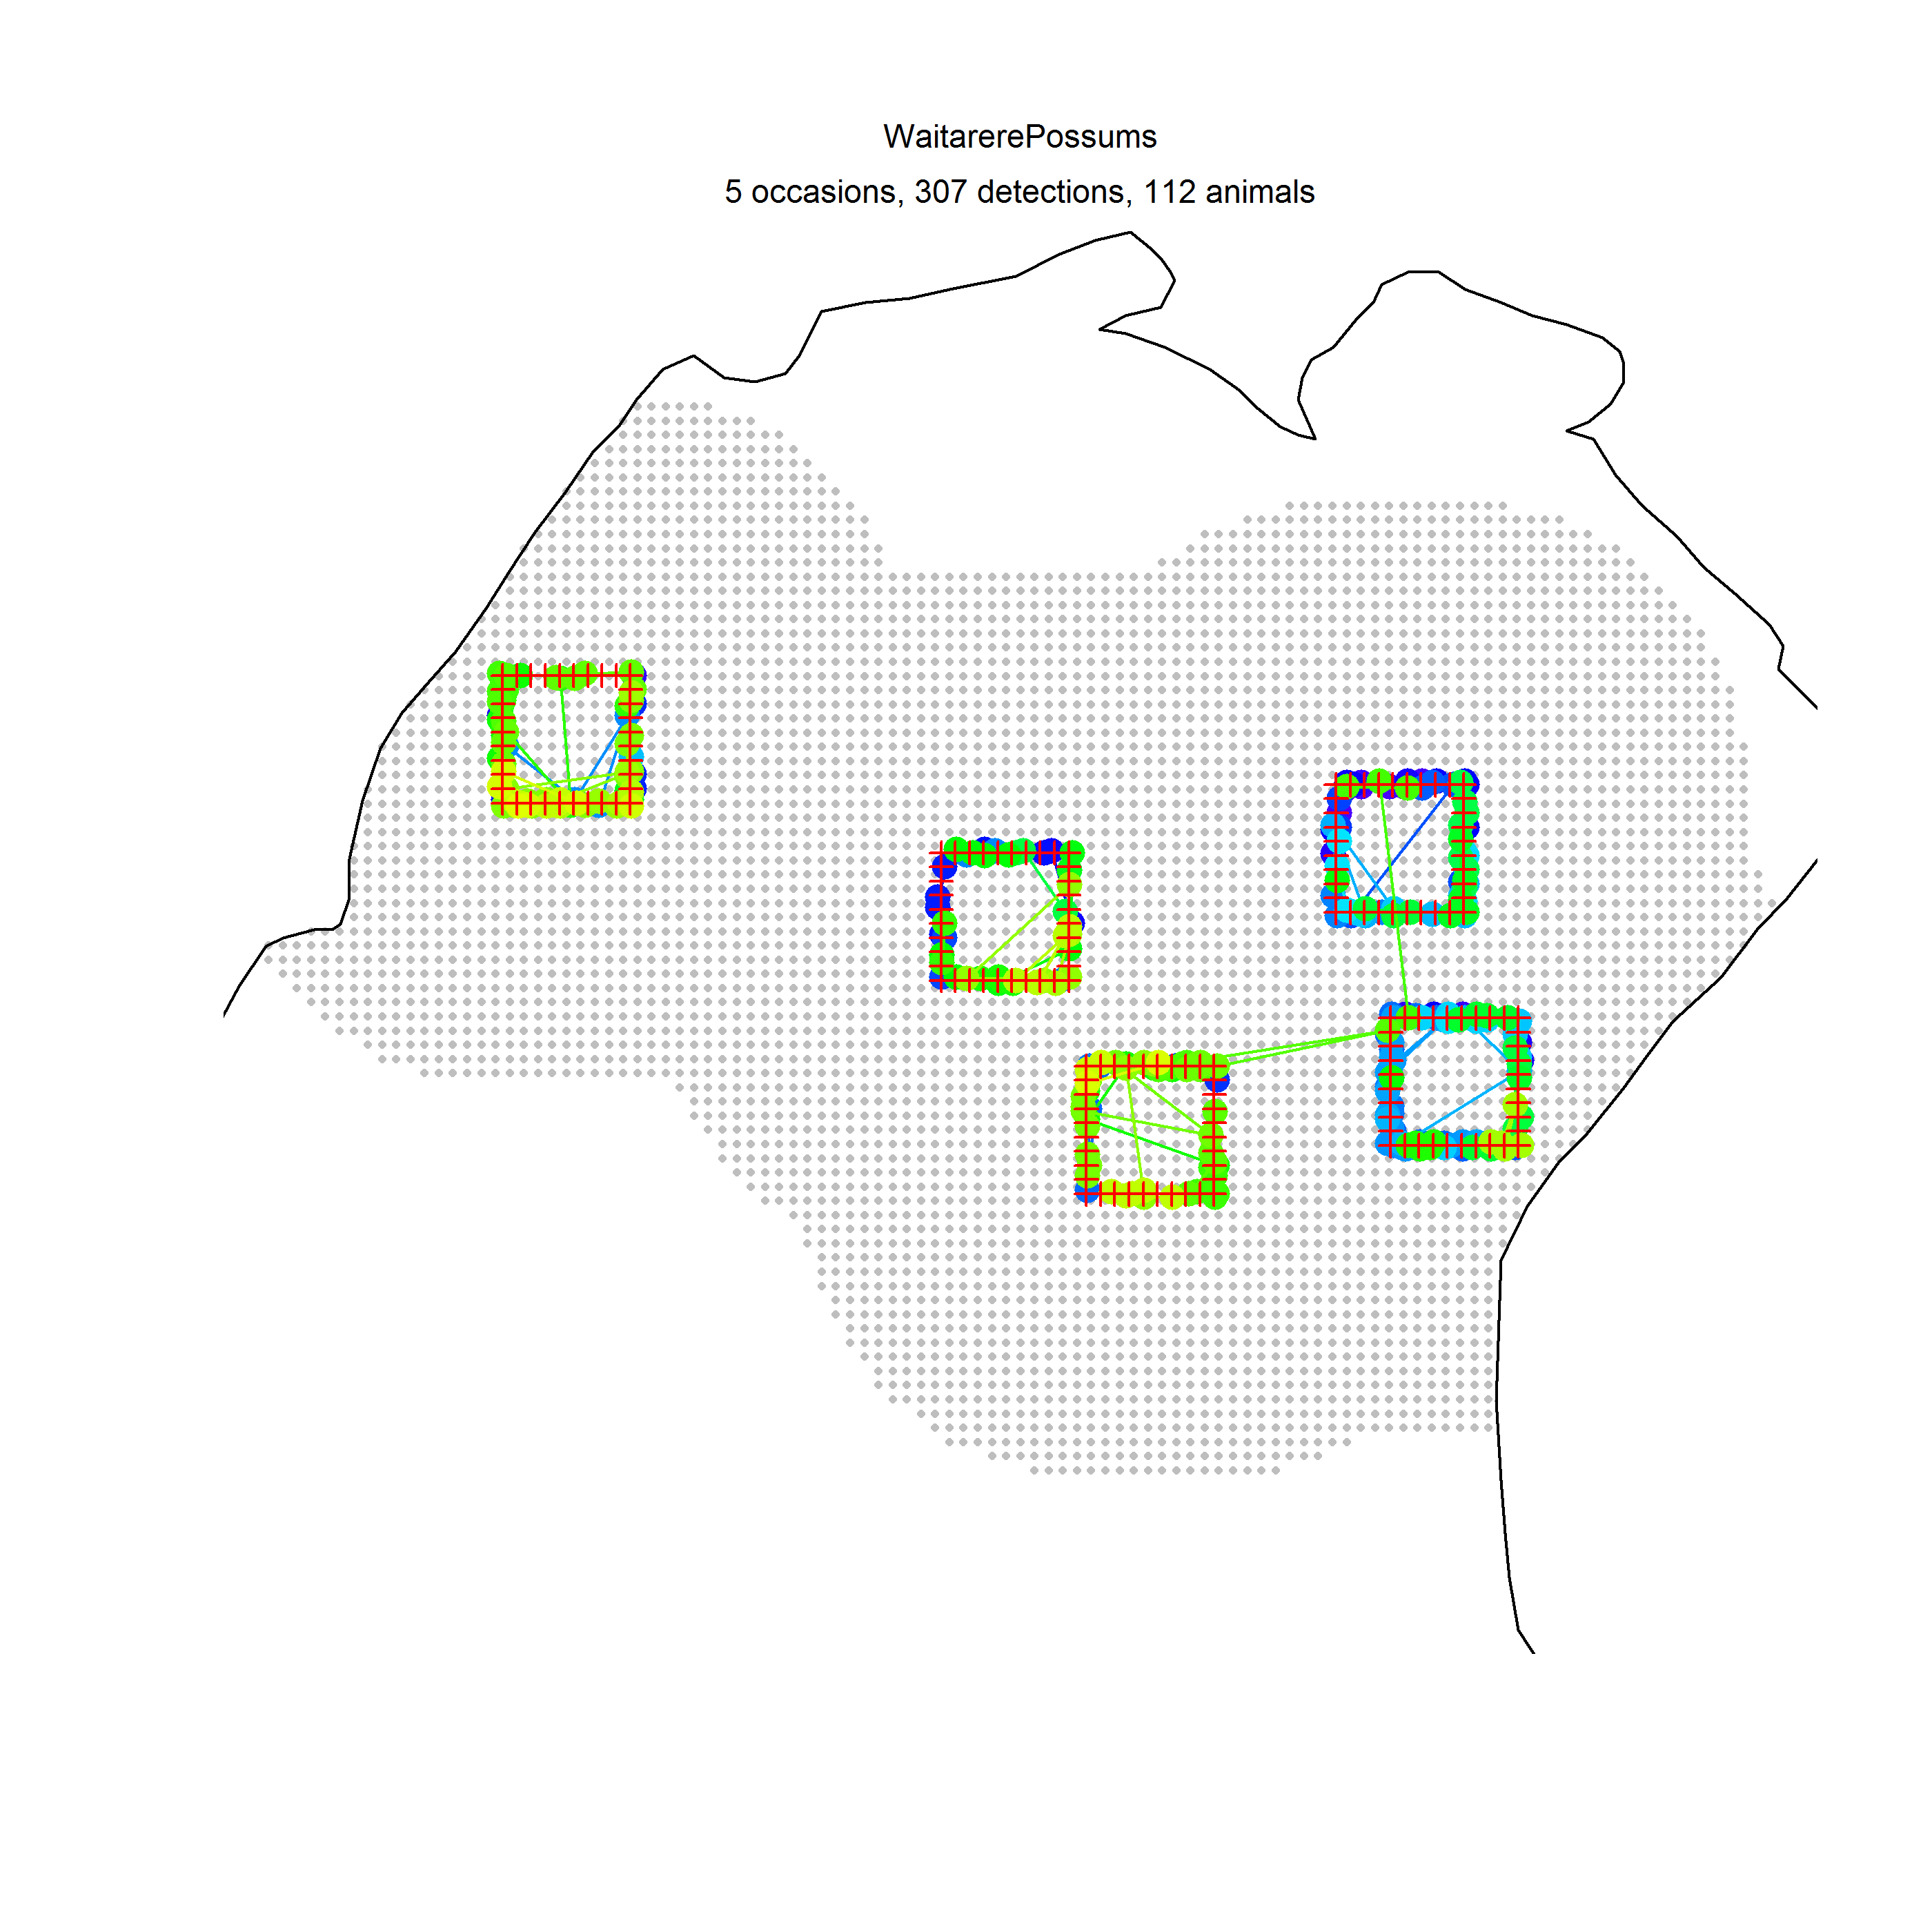
\includegraphics[width=5in]{Ch9-PoisMn/figs/possum.png}
\caption{Trapping grids used in possum study from
  \citet{efford_etal:2005}, data are contained in the \R
package \mbox{\tt secr}
\citep{efford:2011}, refer to the help file \mbox{\tt ?possum} for
additional details of this study.}
\label{poisson-mn.fig.possum}
\end{figure}

The data file \mbox{\tt possumCH} contains 112 encounter histories,
and we analyze those here although the last 8 of those are recaptures
treated as new individuals\footnote{M. Efford, personal communication}.
%Trapping produced
%46 adult females, 33 adult males, 10 immature females and 11
%immature males; sex and/or age were not recorded for 4 individuals
%(M. Coleman unpubl. data).
The encounter process is not strictly a single-catch multinomial process because,
as noted in the \mbox{\tt possum} help file
 ``One female possum was twice captured at two
sites on one day, having entered a second trap after being released;
one record in each pair was selected arbitrarily and discarded.''
which is a similar situation to what might happen in bird mist net
studies, as a bird might fly into a net upon release from another.
If this was a significant problem then it might be worth describing a
model for $n_{ik} = $ the number of captures of individual $i$ during
sample occasion $k$ to make use of all captures. By discarding the two
extra-capture events, we can satisfactorily view these data as
single-catch data, for which \mbox{\tt secr} uses the independent
multinomial likelihood (M. Efford, pers. comm.).

For our Bayesian analysis here, we used a rectangular state-space which
doesn't account for any geographic boundaries of the survey region, but
we note that a habitat mask is included in {\tt secr} and it could be
used in a Bayesian analysis.
%, and we analyze the
%data using that mask in Chapt. \ref{chapt.mle}.
Whether or not we use the mask is
probably immaterial as long as we understand the predictions of $N$ or
$D$ over the water don't mean anything biological and we probably
wouldn't report such predictions. Shortly we will show how to make a
density map that is suitably restricted. The {\bf JAGS} model
specification is based on that of the ovenbird analysis given
previously, and so we don't reproduce the model here. The {\bf R/JAGS}
script called \mbox{\tt SCRpossum} which is in our \mbox{\tt scrbook}
package.
The results are summarized in Tab. \ref{poisson-mn.tab.possum}.



\begin{table}[ht]
\centering
\caption{Results of fitting the independent multinomial observation
  model to the possum trapping data. Strictly speaking, the trapping
  device is a ``single-catch'' trap, and the model represents an intentional
  misspecification.
Posterior summaries were obtained using {\bf JAGS} with
 3 chains, each with 2000 iterations, discarding the first 1000 as
 burn-in, to yield a total of 3000 posterior samples.
}
\begin{tabular}{crrrrrrr} \hline \hline
 parameter & mean &  sd   & 2.5\% & 50\%  & 97.5\% &Rhat& n.eff \\ \hline
D        &  0.000 &  0.000&   0.000 &  0.000 &  0.000 &1.009 &  340\\
Dha      & 1.549  &  0.115&   1.343 &  1.547 &  1.777 &1.009 &  340\\
N        & 235.407&  17.435& 204.000& 235.000& 270.000& 1.009&   340\\
alpha0   &-0.935  &  0.167 & -1.270 & -0.934 &  -0.605& 1.007&   870\\
alpha1   &0.000   & 0.000  & 0.000  & 0.000  &   0.000& 1.001&  2800\\
psi      &0.783   & 0.062  & 0.666  & 0.782  &   0.903& 1.008&   340\\
sigma   &52.020   & 2.675  &47.067  & 51.933 &  57.585& 1.001&  2800
\\ \hline
\end{tabular}
\label{poisson-mn.tab.possum}
\end{table}


The estimated density (posterior mean) is about 1.53 possums/ha.
To obtain the \mbox{\tt secr} results for the equivalent null model, we execute the following command
\begin{verbatim}
secr.fit( capthist = possumCH, trace = F )
\end{verbatim}
which produces (edited) summary output:
\begin{verbatim}
[... some output deleted ...]

Fitted (real) parameters evaluated at base levels of covariates
       link   estimate SE.estimate        lcl        ucl
D       log  1.6988930  0.17352645  1.3913904  2.0743547
g0    logit  0.1968542  0.02256272  0.1563319  0.2448321
sigma   log 51.4689114  2.59981905 46.6204139 56.8216500

[... some output deleted ...]
\end{verbatim}
As we've discussed previously, there are many reasons for why there
might be differences between Bayesian and likelihood estimates.  But
even among likelihood estimates -- any time you run a model there is
some numerical integration going on which requires some specific
choices of how to do the integration (see Chapt. \ref{chapt.mle}).
For now we just observe that the estimated density is certainly in the
ballpark and so too is the estimated $\sigma$.

%%%{\bf XXX RERUN WITH LARGER STATE SPACE XXXX}
%%%%{\bf XXXX TO DO XXXXXX Density MAP XXXXXX}


\section{Acoustic sampling}
\label{poisson-mn.sec.acoustic}

The last decade has seen an explosion of technology that benefits the
study of animal populations. This includes DNA sampling methods that
allow for identification from hair or scat, camera trapping and
identification software that allow efficient sampling of many
carnivores, and the resulting statistical technology that helps us to
make sense of such data \citep{borchers_efford:2008,
  royle_young:2008,efford_etal:2009ecol, gopalaswamy_etal:2012ecol,
  sollmann_etal:2012ecol, chandler_royle:2012}.  One other extremely
promising technology area is that of acoustic sampling using
microphones or recording devices.  That is, instead of having cameras
record data, or humans pick up scat, we can establish an array of
(usually) electronic recording devices which, instead of establishing
a visual identity of individuals, they record a vocal expression of
each individaul.  In this context, \citet{efford_etal:2009ecol}
referred to audio recorders as ``signal strength proximity detectors''
to distinguish them from other types of proximity detections,
including camera traps, which are {\it visual} proximity detector.
Using audio records, the spatial pattern of the {\it signal strength}
at the different microphones can be used for inference about density
\citep{dawson_efford:2009,efford_etal:2009ecol} in the same way as the
spatial pattern of detections is used in the types of SCR models we
have discussed so far.
% XXXX Here you might say that an important distinction is that
% density in this case is "sound sources"
% per area, rather than activity centers per area.
The basic technical formulation of these
models comes from \citet{efford_etal:2009ecol}, and it was applied to
field study of birds by \citet{dawson_efford:2009}. In that study,
recording devices were organized in groups of 4 (in a cross pattern),
% XXXX plot(signalCH) makes it look like a square pattern
with an array of $5 \times 15$ such cross-patterns, seperated by 100 m
(300 total recorder locations).  This data set,
called \verb+signalCH+, % XXXX
is provided with the
\mbox{\tt secr} package along with some sample analyses and help
files.
See \citet{efford_dawson:2010}, a version of the document
\mbox{\tt secr-sound.pdf} that comes with the \mbox{\tt secr} package,
which you can access directly from the main help file (\mbox{\tt
  ?secr}).

Our development here mostly follows \citet{efford_etal:2009ecol}, but
we change some notation to be consistent with our previous material.
Let $S({\bf x}, {\bf u})$ be the strength of a signal emanating from
signal % XXXX
location ${\bf u}$, as recorded by a device at location ${\bf x}$.
Just as ordinary SCR models represent a model of {\it encounter
  frequency} as a function of distance, in acoustic models, the
acoustic SCR model is a model of sound attenuation as a function of
distance.  In particular, the acoustic models assumes that $S$ (or a
suitable transformation) declines with distance $d$ from the origin of
the sound, to the recording device. In the context of spatial sampling
of animals, the origin is the actual location of some individual
animal, and the recording device is something we nailed to a tree, or
put on a stick somewhere, or whatever.  For example, a model of sound
attenuation used by \citet{dawson_efford:2009} is the following:
\begin{equation}
S({\bf x},{\bf u})  = \alpha_{0} + \alpha_{1} d({\bf x},{\bf u}) + \epsilon
\label{poisson-mn.eq.signal}
\end{equation}
% XXXX Does epsilon need a subscript?
where $\epsilon \sim \mbox{Normal}(0, \sigma_{s}^{2})$. In many standard
situations, $S$ will be measured in decibels, which can be any value
on the real line.  In the conduct of acoustic sampling and the
development of custom models for your own situation, it would probably
be helpful to know something about sound dynamics and signal
processing, although we don't know much.  In this model, the
parameters $\alpha_0$, $\alpha_1$ and $\sigma_{s}^{2}$ are to be
estimated. We abbreviate the set of parameters by $\bm \theta$ for short.

We assert that an individual is detected if $S$ exceeds a threshold,
$c$. The reason for introducing this threshhold $c$ is that sound
recorders will always record some
background % XXXX
sound, and so effective use of the
acoustic SCR models requires specification of the threshold of
measured signal below which the record is censored (non-detection
occurs) because the recorded sound it assumed to be background noise.
So we assert that an individual is detected if $S>c$ which occurs with
probability $\Pr(S > c)$, the encounter probability.  To expand on and
formalize this, let $S_{ij}$ be the observed value of $S$ for animal $i$ at
detector $j$.  The encounter probabiliy is $\Pr(S_{ij}>c)$ which is
$\Pr(S_{ij}>c) = 1- \Pr(S_{ij} < c)$, so that, if we standardize the
variate we have
\[
1-\Pr\left( \frac{ (S_{ij}- \mathbb{E}(S))}{\sigma_{s}}  <  \frac{
(c -  \mathbb{E}(S)) }{\sigma_{s}} \right)
\]
This probability % XXXX This sentence is somewhat hard to follow
calculation is the CDF  of a standard normal variate
say $\eta = (S_{ij}- \mathbb{E}(S))/\sigma_{s}$ is
less than the quantity
$\gamma({\bm \theta}) = (c -  \mathbb{E}(S))/\sigma_{s}$
which is a function of all the parameters $\alpha_{0}$, $\alpha_{1}$,
$\sigma_{s}^{2}$ and also the individual location ${\bf u}$ and trap location
${\bf x}$.
We'll identify it by
$\gamma({\bm \theta},{\bf x},{\bf u})$ when we need to be explicit
about those things.
 We can compute
$\Pr(S_{ij}>c) = 1-\Pr(  \eta <
\gamma({\bm \theta}, {\bf x},{\bf u}))$ easily using any software
package including {\bf R} which has a standard function, \mbox{\tt
  pnorm}, for computing the normal cdf.
To be more precise, we'll use the $\Phi()$ to represent the normal
cdf. Therefore, an individual is encountered whenever $S_{ij}>c$ which
happens with probability
$\Pr(S_{ij}>c) = 1-\Phi( \gamma({\bm \theta}, {\bf x},{\bf u}) )$.

Naturally this quantity should depend on {\it where} an individual is
located at the time of recording
-- what we call it's instantaneous location, say ${\bf u}$, to
distinguish it from it's
 home-range center ${\bf s}_{i}$ (but we outline a model below that
 contains both ${\bf u}$ and ${\bf s}$),
and also the trap ${\bf x}$, so we
 index the quantity $\gamma$ by those two quantities, in
addition to the parameters $\alpha_{0}$, $\alpha_{1}$ and $\sigma_{s}$.
The probability of detection is therefore
\[
p_{ij} = p(\alpha_0, \alpha_1, \sigma | {\bf x}_{j}, {\bf u}_{i} ) = 1- \Phi( \gamma(\cdot))
\]
where
 ${\bf u}_{i}$ is the instantaneous location of individual $i$ and
${\bf x}_{j}$ is the location of trap $j$.  We'll suppose here that
the random variables ${\bf u}_{i}$ have state-space ${\cal S}$.

How do we interpret this probability? Well, two things have to happen
for an individual to be encountered by a trap:
(1)  it has to  vocalize; (2)
the microphone has to record a signal $>c$. These two things
together are a product of biological and environmental factors which
could include time of day, wind direction and speed, or maybe rain,
humidity and other things. The bottom line is a lot of factors are
balled up in whether or not the microphone records a sound greater
than the threshhold.  In addition,
we have to suppose that the vocalizations
are reconcilable and reconciled successfully by the
investigator.

The observations from an acoustic survey are the signal strength
measurements, and
the likelihood of the observed signal strength
from individual $i$ at detection
device $j$ can be specified by noting that
the
likelihood is the normal pdf for the observed signal {\it if} the
signal strength is $>c$ and, otherwise, the contribution to the
likelihood is $\Phi(\gamma(\cdot))$ (see Eq. 8 from \citet{efford_etal:2009ecol}):
\[
\Pr(S_{ij}| {\bf u}_{i} ) = \Phi( \gamma( \cdot) )^{1-1(S_{ij}>c)}
\mbox{Normal}(S_{ij};\alpha_{0},\alpha_{1},\sigma_{s},{\bf x}_{j},{\bf
u}_{i})^{1(S_{ij}>c)}
\]
\begin{comment}
XXXX Note: I think this formula is wrong. Why shouldn't this be a
  truncated-Normal PDF? XXXXXX i.e., $Pr(S|S>c)$? It should be, but
  then by ``capturing'' the guy, this happens with probability Pr(S>c)
and so that cancels from the denominator.
i.e., the likelihood is really:
Pr(S|S>c and S>c) =
[ Pr(S)/Pr(S>c) ] * Pr(S>c)    = Pr(S)

I don't think Efford et al. explained the origins of this formula very well!
\end{comment}

We can use this as the basis for constructing the binomial-form of the
likelihood as we did in Chapt. \ref{chapt.mle}, which involves the
number of individuals not encountered, $n_{0}$.  The probability that
an individual is {\it not} captured is equal to the probability that
its signal strength doesn't exceed $c$ at any microphone.  The
probability of not being captured at a microphone ${\bf x}_{j}$ is:
\[
1-p_{{\bf u},j} = \Phi( \gamma(\cdot) )
\]
and therefore the probability of not being captured at any microphone is:
\[
\Pr(\mbox{all } S < c | {\bf u}) = \prod_{j=1}^{J} ( 1-p_{{\bf u},j} )
= \prod_{j=1}^{J} \Phi( \gamma(\cdot, {\bf x}_{j}, {\bf u}) )
\]
and therefore the marginal probability of not being captured is
\[
\pi_{0} = [ \mbox{all }  S < c | {\bm \alpha}] =
\int_{{\cal S}}
 \left\{
\prod_{j=1}^{J} \Phi( \gamma( {\bm \theta}, {\bf x}_{j}, {\bf u}) )
 \right\}
 d{\bf u}
\]
which can be used to construct the binomial form of the likelihood as
we did in Chapt. \ref{chapt.mle} (see Eq. \ref{mle.eq.binomialform}).




\begin{comment}


The probability that signal strength exceeds ``c'' at one or more
detectors is:
\begin{verbatim}
p_{dot}(X) = 1- \prod_{k=1}^{K}(   1-\phi(  gamma(X,k)) )
\end{verbatim}

\end{comment}

\subsection{Implementation in \mbox{\tt secr}}

Fitting acoustic encounter models in \mbox{\tt secr} is no more
difficult than other SCR models. There is a handy manual (\mbox{\tt
  secr-sound.pdf}) with examples \citep{efford_dawson:2010} which
comes with the \mbox{\tt secr} package.  The basic process is that
\mbox{\tt make.capthist} will make a \mbox{\tt capthist} object from a
3-d % XXXX I wonder if I write 3D sometimes?? I'll check
encounter array -- which is a binary array indicating whether each
individual was detected or not at each recorder/microphone. In the
case of acoustic data, \# occasions = 1 because the recorders obtain
data for a single interval.  The ``signal'' attribute of the \mbox{\tt
  capthist} object contains the signal strength in decibels.  The best
way to include the signal attribute is to use \mbox{\tt make.capthist}
in the usual way, providing it with the encounter data and trap data
and, in addition, the variable ``cutval'' (which is $c$ in our
notation above) and then provide the signal strength data as an extra
column of the \mbox{\tt capthist} object.  See \mbox{\tt
  ?make.capthist} for details.
\begin{comment}
``Signal strengths may be
provided in the fifth (fmt = trapID) or sixth (fmt = XY)
columns. Detections with signal strength missing (NA) or below
'cutval' are discarded.''


The ``ovensong'' data set in \mbox{\tt secr} has an example (\mbox{\tt
  ?ovensong}) which is from \citep{dawson_efford:2009}.

You have to set the \mbox{\tt cutval}..... which we called $c$ above.
Otherwise fitting a model in \mbox{\tt secr} goes the same as for any
other model. For the \mbox{\tt ovensong} example in \mbox{\tt secr}
has the following code:


## apply signal threshold
signalCH.525 <- subset(signalCH, cutval = 52.5)

## Not run:
## models with and without spherical spreading
omask <- make.mask(traps(signalCH), buffer = 200)
ostart <- c(log(20), 80, log(0.1), log(2))
ovensong.model.1 <- secr.fit( signalCH.525, mask = omask,
    start = ostart, detectfn = 11 )
ovensong.model.2 <- secr.fit( signalCH.525, mask = omask,
    start = ostart, detectfn = 10 )

\end{comment}



\subsection{Implementation in {\bf BUGS}}

We don't know of any Bayesian applications of acoustic SCR models,
although we imagine that implementation of such models in the {\bf
  BUGS} engines should be achievable.  It seems easy enough to write
down a general hierarchical model that would accomomdate sampling on
repeated occassions. Let ${\bf s}_{i}$ be the home range center, and
let ${\bf u}_{ik}$ the instantaneous location of individual $i$ during
sample occasion $k$ (see Chapt. \ref{chapt.search-encounter} for
similar models). The model for ${\bf u}_{ik}$ can be specified
conditional on ${\bf s}_{i}$. For example, we could assume that ${\bf
  u}_{ik}$ are bivariate normal draws with mean ${\bf s}_{i}$ and some
variance $\sigma_{u}^{2}$. Then, conditional on ${\bf u}_{ik}$ an
individual produces a signal according to the signal attenuation model
(Eq. \ref{poisson-mn.eq.signal}), or perhaps some other model. Then we
generate the binary encounter data by truncating the observed signal
at $c$. This general model then is an example of an SCR model in which
parameters of a movement model are identifiable
(see Sec. \ref{modeling.sec.characterization})
 because
there is direct information about movement outcomes from the sampling
method, unlike other types of encounter methods (e.g., camera traps)
for which animal locations are restricted to a set of fixed, pre-determined
points where traps are located.  Other types of SCR methods allow for
movement information too, including some of the search-encounter
models (Chapt. \ref{chapt.search-encounter}).


Instead of developing a Bayesian version of this model here,
we leave it to the reader to
explore simulating data and devising a Bayesian implementation of the
acoustic model in one of the {\bf BUGS} engines.
% XXXX I wonder if we could show some generic BUGS code for this,
% without supplying simulated data? Below is a hack at this:
Note that for a
single occasion, you can simulate the data using the two stage model
(having both ${\bf s}$ and ${\bf u}$) or you can simulate ${\bf u}$
uniformly at the start.

\begin{comment}
# ANDY, is this about right???
model {
  # ignoring loops
  u[i,1] ~ dunif(xlim[1], xlim[2])
  u[i,2] ~ dunif(ylim[1], ylim[2])
  mu[i,j] <- alpha0 + alpha1*d[i,j]
  S[i,j] ~ dnorm(mu[i,j], 1/sigma^2)T(c,Inf) # JAGS has this T() truncation feature
  gamma[i,j] <- (c - mu[i,j])/sigma
  p[i,j] <- 1 - pnorm(gamma[i,j], 0, 1) # JAGS has pnorm() function
  y[i,j] ~ dbern(p[i,j])
}
\end{comment}


\begin{comment}
  XXXX It seems like there are a lot of general considerations that
  the practitioner will need to think about. For example, these
  acoustic models assume that the survey is conducted during an
  ``instant'' in time right? You offered a way of dealing with
  movement, but what if a bird sings twice during a time interval?
  If they are different songs, wouldn't this model incorrectly think
  that they are two distinct birds?

  Another biggie is how do you interpret this density estimate? It
  doesn't account for the probability that an individual vocalizes
  right? Don't we somehow need an estimate of that if we want
  animals/area instead of sounds/area? I don't think alpha0 can be
  interpretted in this way, right?

  I guess Dawson and Efford get at some of this in their abstract, where
  they say ``The method requires that
  individuals detected at the same place are acoustically
  distinguishable and all individuals vocalize
  during the recording interval, or that the per capita rate of
  vocalization is known.'' We should probably mention this.

  Two other things: (1) We need to briefly discuss ``spherical
  spreading''. D and E say this about Eq1: The second term describes the spherical spread of sound energy,
and the final term represents log-linear attenuation from all other
causes (b1 < 0).We set lS = b0 for d < 1,when spherical spreading
generally does not apply (Wiley & Richards 1982), thus avoiding
computational problems at d = 0.

And (2) we need to cite some of Tiago's papers on this stuff.
\end{comment}


\subsection{Other types of acoustic data}

\citet{efford_dawson:2010} noted that various other types of acoustic
data might arise for which SCR-like models would be
useful\footnote{Some of the following is also related to material
  presented by D.L. Borchers at the ISEC 2012 conference in Norway.}.
For example, we could have devices that measure the {\it time of
  arrival} of a queue of some sort.
Another example is that where we measure {\it direction} to a queue
from multiple devices and do, effectively, a type of statistical
triangulation to the multiple but unknown number of sources.  This has
direct relevance to types of double or multiple-observer sampling that
people do in field studies of birds. Normally 2 observers stand in
close proximity and record birds, reconciling their detections after
data collection. An SCR-based formulation of the double-observer
method has two observers (or more) standing some distance apart, e.g.,
50 or 100 meters,  and marking individual birds on a map (or at
least a direction) and a time of detection.  The SCR/double-observer
method could be applied to such data.



\section{Summary and Outlook}

In this chapter we extended SCR models to accommodate alternative
observation models, including Poisson and multinomial models.  Along
with the binomial model described in Chapt. \ref{chapt.scr0}, this
sequence of models will accommodate a substantial majority of
contemporary spatial capture-recapture problems, including
the 4 main types of encounter data:
binary encounters, multinomial trials from ``multi-catch'' and
``single-catch'' \citep{efford:2004, efford:2011, royle_gardner:2011}
trap systems, and Poisson encounter frequency data from devices that can
record multiple encounters of the same individual at a device.  We
summarize the standard observation models and the corresponding
\mbox{\tt secr} terminology in Table \ref{poisson-mn.tab.models}.  What
we refer to as search-encounter (or area-search) models (see
Chapt. \ref{chapt.search-encounter}) are distinct
from most of the other classes in that the observation location can
also be random (in contrast to traps, where the location is fixed by
design). This auxiliary data is informative about an intermediate
process related to movement \citep{royle_young:2008}.

\begin{table}[ht]
\centering
\caption{
Different observation models, where we discuss then in this
  book, and what the corresponding \mbox{\tt secr} terminology is
}
\begin{tabular}{lll}
\hline \hline
observation model & Where in this book?  &  \mbox{\tt secr} name  \\ \hline
Bernoulli         & Chapt. \ref{chapt.scr0}    &   \mbox{\tt proximity} \\
Poisson           & Sec. \ref{poisson-mn.sec.poisson} & \mbox{\tt count} \\
Multinomial (ind) & Sec. \ref{poisson-mn.sec.multinomial} & \mbox{\tt  multi-catch} \\
Multinomial (dep) & Sec. \ref{poisson-mn.sec.singlecatch} & \mbox{\tt  single-catch} \\
Acoustic          & Sec. \ref{poisson-mn.sec.acoustic}
   &  \mbox{\tt signal}  \\
Search-encounter      & Chapt. \ref{chapt.search-encounter}  &
\mbox{\tt polygon} (in part) \\ \hline
\end{tabular}
\label{poisson-mn.tab.models}
\end{table}

There is a need for other types of encounter models that arise in practice. We
identify a few of them here, although we neglect a detailed
development of them at the present time or, in some cases, put that
off until later chapters: (1) Removal systems -- Sometimes traps kill
individuals and SCR models can handle that. This can be viewed as a
kind of open model, with mortality only, and we handle such models (in
part) in % XXXX Except, no recaptures can occur, so this seems
         % impossible in SCR. Or, it seems like an interesting
         % research avenue.
Chapt. \ref{chapt.open};  (2) There are models for which only specific
summary statistics are observable
\citep{chandler_royle:2012,sollmann_etal:2012ecol} which we cover in
Chapts. \ref{chapt.scr-unmarked}- \ref{chapt.partialID}; (3) We can
have multiple observation methods working together as in
\citet{gopalaswamy_etal:2012ecol} which we summarize in Sec. XXXXX.

There remains much research to be done to formalize models for certain
observation systems. For example, while we think one will usually be
able to analyze single-catch systems using the multi-catch model, or
even the Bernoulli model if encounter probability is sufficiently low,
a formalization of the single-catch model would be a useful
development and, we believe, it should be achievable using one or
another of the {\bf BUGS} engines.  In addition, classical ``trapping
webs'' \citep{anderson_etal:1983, wilson_anderson:1985b,
  jett_nichols:1987, parmenter_etal:1989,link_barker:1994}
have been around for quite
some time and it seems like they are amenable to formulation as a type
of SCR model although we have not pursued that development simply
because trapping webs are rarely used in practice.




\chapter{
Sampling Design
}
\markboth{Sampling design}{}
\label{chapt.design}

\vspace{.3in}


Statistical design is recognized as an important component of animal
population studies \citep{morrison_etal:2008,
  williams_etal:2002}. There are probably few to no field biologists
who have never been in the situation where a problem with data could
be traced back to some flaw in study design.  Commonly, design is
thought of in terms of number of samples to take, when to sample,
methods of capture, desired sample size (of individuals), power of
tests, and related considerations.  In the context of spatial sampling
problems, where populations of mobile animals are sampled by an array
of traps or devices, there are a number of critical design elements.
Two of the most important ones are the spacing and configuration of
traps (or sampling devices) within the array.  While conceptual and
heuristic design considerations have been addressed by a number of
authors (e.g., \citealp{nichols_karanth:2002}, Chapt. 11), little
formal analysis focused on spatial design of arrays has been carried
out. \citet{bondrup-nielsen:1983} investigated the effect of trapping
grid size (relative to animal home range area) on density estimates using a simulation
study and some authors have addressed trap spacing and configuration
by sensitivity ``re-analysis'' (deleting traps and reanalyzing;
\citealp{wegge_etal:2004, tobler_etal:2008}). The scarcity of
simulation-based studies looking at study design issues is surprising,
as it seems natural to evaluate prescribed designs by Monte Carlo
simulation in terms of their accuracy and precision.

Theoretically optimal (or extremely good) designs are useful to study
in order to understand how factors influence the design
problem. However, often field studies face logistic difficulties,
especially when dealing with wide-ranging, rare and cryptic species
like large carnivores. The need to sample large areas with limited
resources often forces researchers to compromise between a study
design that is optimized for statistical inference and a study design that is
logistically viable or efficient. In such studies, traps are often placed along
roads or rivers where a large number of traps can be accessed with
relative ease. Unless the study site is crossed by a network of roads
or waterways, this will lead to a sampling design that is much more
'linear' compared to an area-based design where traps are spread out
uniformly over the study site.

In this chapter we recommend a general framework for evaluating
specific design choices for SCR studies based on Monte Carlo
simulation of specific design scenarios based on trade-offs between
available effort, funding, logistics and other practical
considerations -- what we call {\it scenario analysis}.  Many study
design related issues such as how long to survey in order to obtain
sufficient data, can be addressed with preliminary field studies that
will give you an idea of how much data you can expect to collect
within a unit of effort (a camera trap day or a point count survey,
for example).  But it is also always useful to perform scenario
analysis based on simulation before conducting the actual field survey
not only to evaluate the design in terms of its ability to generate
useful estimates of things, but also so that you have an expectation
of what the data will look like as they are being collected. This
gives you the ability to recognize some pathologies and possibly
intervene to resolve issues before they render a whole study
worthless. Suppose you design a study to place 40 camera traps based
on your expectations of parameter values you obtained from a careful
review of the literature, and simulation studies suggest that you
should get 3-5 captures of individuals per night of sampling. In the
field you find that you're realizing 0 or 1 captures per night and
therefore you have the ability to sit down and immediately question
your initial assumptions and possibly take some remedial
action. Simulation evaluation of design {\it a priori} is therefore a
critical element of any field study.

%Yet another design that has been
%proposed for regular capture-recapture studies is that of a trapping
%web (DESCRIBE). {\bf XXXX Maybe not? XXXX} In the second part of this
%chapter we look into the performance of these trap arrangements.


While we recommend scenario analysis as a general tool to understand
your {\it expected data} before carrying out a spatial
capture-recapture study, it is possible to develop some heuristics and
even analytic results related to the
broader problem of model-based spatial design
\citep{muller:2007} using an explicit objective function based on the
inference objective.  We outline an approach in this chapter where we
identify a variance criterion that depends on the configuration of
trap locations, and we optimize that variance criterion over the
design space (the collection of all possible designs of a given
size). While there is much work to be done on developing this idea, we
believe that it provides a general solution to any type of design
problem where the space of candidate trap locations is well-defined. 
% XXXX RC says: I would beef this paragraph up. You write a lot about the
% simulation-based scenario-analysis, but just 1 sentence about the
% analytical approach which seems very promising.


% XXXX RC says: Doesn't Murray have some paper where he discuss design
% issues? Or where did the 2sigma rule come from? Also, you might want
% to cite Rahel/Beth's paper on design here.

\section{General Considerations}

Many biologists have experience with the design of natural resource
surveys from a classical perspective
\citep{thompson:2002,cochran:2007}, a key feature of which involves
sampling space. That is, we identify a sample frame comprised of
spatial units and we sample randomly (or by some other method, such as
generalized random tesselation stratified (GRTS) sampling \citep{stevens_olsen:2004})
those units and measure some attribute. The resulting inference
applies to the attribute of the sample frame. There are some distinct
aspects of the design of SCR studies which many people struggle with
in their attempts to reconcile SCR design with classical survey design
problems.

\begin{comment}
\subsection{Model-based not design-based}

{\bf XXX ANDY: I find this little subsection hard to understand; maybe it needs some mroe elaborating. I really like the following one though. XXXXXX

XXX Reply: Andy sez: I agree, not worth going here.
}
We take a model-based approach to the design of SCR studies. That is,
we seek design features -- spatial arrangements of samples -- which we
expect to produce estimators of model parameters that have a
satisfactory desired level of precision.

Classical finite-population sampling is often ``design-based'' which
means properties of estimators (bias, variance) are evaluated over
repeated realizations of the {\it sample}. The sample is random, but
the attribute being observed is not. However, in the SCR modeling
framework properties of our estimators are distinctly model-based.  We
evaluate estimators (usually) or care only about a {\it fixed} sample,
averaged over realizations of the underlying process and data we might
generate. This is a classical parametric frequentist idea which we
think makes as much sense as a Bayesian too.
\end{comment}



\subsection{Sampling space or sampling individuals?}

A fundamental question in any sampling problem is what is the sample
frame -- or the population we are hoping to extrapolate too. In the
context of capture-recapture studies, it is tempting to think of the
sample frame as being spatial (the space within ``the study area'',
tiled into quadrats perhaps).  Clearly SCR models involve a type of
spatial sampling -- we have to identify spatial locations for traps,
or arrays of traps.  However, unlike conventional natural resource
sampling the attribute we measure is {\it not} directly relevant to
the {\it sample location}, such as where we place a trap and,
therefore, it may not be sensible to think of the sample frame as
being comprised of spatial units.
% XXXX RBC says: I think it is worth discussing the situation in which
% a researcher wants to know density (or variation in density) within
% some well-defined area, like a park or on an island. In that case,
% they very well might want to think about sampling some finite
% space. RBC says later: Okay, see that you discuss this issue in
% depth below, but you might want to briefly say something about it
% here too XXXX
On the other hand,
capture-recapture studies clearly obtain a sample of {\it individuals}
and SCR models are models of {\it individual} encounter and space use.
Therefore, it is more natural to think of the sample frame as a list
of $N$ individuals, deterimined by the definition of the state-space,
or a subset of the state-space, i.e., the study-area, but the number
$N$ is unknown.
%You can think of it this way: the study
%area deterimines the collection of individuals that we care about for
%management or whatever, but additional individuals might be exposed to
%sampling.

Spatial sampling in SCR studies is important, but only as a device for
accumulating individuals in the sample from which we can learn about
their inclusion probability. That is, we're not interested in any
sample unit attribute directly but, rather, we use spatial units as a
means for sampling individuals and obtaining individual level
encounter histories.
It makes sense in this context
that we should want to choose a set of spatial sample units that
provides an adequate sample size of individuals, perhaps as many as
possible. The key technical consideration as it relates to spatial
sampling and SCR is that arbitrary selection of sample units has a
side-effect that it induces unequal probabilities of inclusion into
the sample and so we must also learn about these unequal probabilities
of sample inclusion as we obtain our sample.

The fact that SCR sampling induces unequal probabilities of sampling
is consistent with the classical sampling idea of Horvitz-Thompson
estimation (see
\url{http://en.wikipedia.org/wiki/Horvitz%E2%80%93Thompson_estimator})
which has motivated capture-recapture models similar to SCR
\citep{huggins:1989, alho:1990}.  In the Horvitz-Thompson framework,
the sample inclusion probabilities are usually fixed and
known. However, in all real animal sampling problems they are
unknown because we never know precisely where each individual lives
and therefore cannot characterize its encounter probability.
Therefore, we have to estimate the sample inclusion probabilities
using a model.  SCR models achieve this effect formally, using a
fully model-based 
approach based on a model that accounts for the
organization of individual activity centers and trap locations.
This notion of Horvitz-Thompson estimation suggests that perhaps we
should consider designing SCR studies based on the H-T variance
estimator as a design criterion. We discuss this a little bit later
in this chapter.

\subsection{Focal population vs. state-space}

In SCR models we make a distinction between the focal population --
the population of individuals we care about -- and those
of the state-space,
which we are required to prescribe in order to fit SCR models.
These are not the same thing. The geographic scopt of the population
of inference is
region within which animals live that you care about in your study --
let's call this ``the study area''.  This is often prescribed for
political reasons or legal reasons (e.g. a National Park). To intitiate a study, or perhaps
motivating the study, you have to draw a line on a map to delineate a
study area, although often it is difficult to draw this line, and
where you draw it is not so much a statistical/SCR issue.  On the
other hand, you need to prescribe the state-space to define and fit an
SCR model. This is the region that contains individuals that you {\it
  might} capture. This is different from the study area in most cases.
To design a study, you need a well-defined study area, but the
state-space will also be relevant to efficient distribution of traps,
and other considerations.

% XXXX RBC says: the next two paragraphs are great
It is helpful to think about this distinction operationally. We define
our study area a priori.  As a conceptual device, we might think of
this as the area that, given an infinite amount of resources, we might
wall-off so that we can study a real closed population. This 'study
area' should exist independent of any model or estimator of some
population quantity. i.e., the subject-matter context should determine
what the study area is. Given a well-defined study area, we use some
method to arrange data collecting devices within this study area. The
method of arrangement can be completely arbitrary but, naturally, we
want to choose arrangements of traps that are better in terms of
obtaining statistical information from the data we wind up collecting.

Lets face it -- It's quite a nuisance that animals move around and
this makes the idea of a spatial study area kind of meaningless in
terms of management in most cases. Wherever you draw a line on a map,
there will be animals who live mostly beyond that line that will
sometimes be subjected to your study.  One of the benefits of SCR
models is they formalize the exposure and contribution of these
individuals to your study. That is a good thing. Thus, you can
probably be a bit sloppy or practical in your definition of ``the
study area'' and not worry too much.



\section{Study design for (spatial) capture-recapture}

The importance of adequate trap spacing and overall configuration of
the trapping array has long been discussed in the capture-recapture
literature.  A heuristic based on recognizing the importance of
typical home range sizes \citep{dice:1938, dice:1941} and thus being
able to obtain information about home range size is that traps should
be spaced such that the array of available traps exposes as many
individuals as possible but, at the same time, individuals should be
captureable in multiple traps. Thus, good designs should generate a
high sample size $n$
(i.e., the number of individuals captured) % XXXX RBC add this
and a large number of spatial recaptures.  These
two considerations trade-off in building designs.  On one hand, having
a lot of traps very close together should produce the most spatial
recaptures but produce very few unique individuals captured (assuming
that studies are limited in the total number of sampling devices they
can deploy). On the other hand, spreading the traps out as much as
possible, in a nearly systematic or regular design, should yield the
most unique individuals.  We will formalize this trade-off later, when
we consider formal model-based design of SCR studies.


Traditional CR models require that all individuals in the study area
have a probability $>$ 0 of being captured, which means that the trap
array must not contain ``holes'' large enough to contain an animal's
entire home range \citep{otis_etal:1978}. This ``assumption'' is
imposed in order that a precise area can be used for defining the
population, and for calculation of density. 
% XXXX The non-spatial CR assumption of "no holes" should be
% emphasized heavily. I suggest adding a few sentence about why
% non-spatial models require this assumption, and what the
% consequences of violating it are. And then talk about how hard it is
% to enforce when studing big animals.
As a consequence, trap
spacing should be on the same order as the radius of a typical home
range (e.g., \citealp{dillon_kelly:2007}).  For example, imagine a
camera trap study implemented in South America with the objective to
survey populations of both jaguars and the much smaller
ocelots
({\it Leopardus pardalis}). % XXXX What's our policy on scientific names?
Ocelots also have much smaller home ranges and therefore
should require closer trap spacing than the large wide-ranging
jaguars.  Where approaches such as MMDM are used in combination with
traditional CR models to obtain density estimates (see
Chapt. \ref{chapt.closed}), trap spacing also has a major effect on
movement estimates, since it determines the resolution of the
information on individual movement \citep{parmenter_etal:2003,
  wilson_anderson:1985b}. If trap spacing is too wide, there is little
to no information on animal movement because most animals will only be
captured at one trap \citep{dillon_kelly:2007}. In addition, only a
trapping grid that is large relative to individual movement can
capture the full extent of such movements, and researchers have
suggested that the grid size should be at least four times that of
individual home ranges to avoid positive bias in estimates of density
\citep{bondrup-nielsen:1983}.  This recommendation originated in small
mammal trapping, and it should be relatively easy to follow when
dealing with species covering home ranges $<$ 1 ha. However, translated
to large mammal research, this can entail having to cover several
thousands of square kilometers -- a logistical and financial challenge
that few projects could realistically tackle.

Holes in the study area are of no concern in SCR studies.  As a
practical matter, some animals within the study area might have
vanishingly small probability of being included in the sample, i.e.,
$p \approx 0$, the nice thing about SCR models is that $N$ is
explicitly tied to the state-space, and not the traps which expose
them to encounter.  Within an SCR model, extending inference from the
sample to individuals that live in these holes represents an
extrapolation (prediction of the model outside the range of the data),
but one that the model is capable of producing because we have
explicit declarations, in the model, that it applies to any area
within the state-space (the state-space is a part of the model!), even
to areas where we can't capture individuals because we happened to not
put a trap near them. Conversely, ordinary capture-recapture models
only apply to individuals that have encounter probability that is
consistent with the model being considered. Presumably, the existence
of a hole in the trap array would introduce individuals with $p=0$,
which is not accommodated in those models.


Whereas traditional CR studies are concerned with the number of
individuals and recaptures and with satisfying the model assumption of
all individuals having some probability of being captured, in spatial
capture-recapture we are looking at an additional level of
information: We need spatially spread out captures and
recaptures. That means, it is not enough to recapture an individual,
but we need to recapture at least some individuals at several
traps. Therefore, in general, design of SCR studies boils down to
obtaining three bits of information: total unique
individuals captured,
total number of recaptures
informative about baseline encounter
rate, and spatial recaptures, informative about $\sigma$. Most SCR
design choices wind up trading these three things against each other
to achieve some optimal (or good) mix. So for example if we sample a
very small number of sites a huge number of times then we can get a
lot of recaptures but only very few spatial ones, and few unique
individuals etc.  This need for spatial recaptures may appear as an
additional constraint on study design, but actually, SCR studies are
much less restricted than traditional CR studies, because of the way
animal movement is incorporated into the model: $\sigma$ is estimated
as a specified function of the ancillary spatial information collected
in the survey and the capture frequencies at those locations and this
function is able to make a prediction across distances even when these
are latent, including distances larger than the extent of the trap
array. When there is enough data across at least some range of
distances, the model will do well at making predictions at unobserved
distances. The key here is that there needs to be `enough data across
some range of distances', which induces some constraint on how large
our overall trap array must be to provide this range of distances
(e.g., \citealp{marques_etal:2011}). We will review the flexibility of
SCR models in terms of trap spacing and trapping grid size in the
following section.


\section{Trap spacing and array size relative to animal movement}


% XXXX RBC says: Hard-core Bayesians might want you to say that you
% did a frequentist evaluation of a Bayesian estimator.
Using a simulation study, \citet{sollmann_etal:2012} investigated how
trap spacing and array size relative to animal movement influence SCR
parameter estimates and we will summarize their study here. They
simulated encounter histories on an $8 \times 8$ trap array with
regular spacing of 2 units, using a binomial 
observation model with
Gaussian hazard encounter model, across a 
range of values for the movement parameter $\sigma^*$. We refer to the
movement parameter as $\sigma^*$ here, because
\citet{sollmann_etal:2012} use a slightly different parametrization of
SCR models, in which $\sigma^*$ corresponds to $\sigma\times\sqrt{2}$.

{\bf XXXX ANDY: I am totally blanking here: We formulated the model so
  that the distance function was d2/sig2. That means $\sigma^*$ =
  $\sigma\times\sqrt{2}$, right? It was different before but I think
  now it's right. If I got it wrong, let me know and I'll fix
  it. Sorry!! XXXXXXXXXXXXXXXXXXXXXXXXXXXXXXXXXX }
{\bf XXX Andy sez: I think this is right!}

In Sec. \ref{scr0.sec.implied} we pointed out that under the bivariate
normal (or half-normal) detection model $\sigma$ can be converted into
an estimate of the 95 \% home range or ``use area'' around
$s_i$. Based on this transformation, values for $\sigma^*$ were chosen
so that there was a scenario where
the trap array was smaller than a single individual's home range,
i.e. trap spacing was narrow relative to individual movements
($\sigma^*$ = 5), a scenario where spaces between traps were large
enough to contain entire home ranges ($\sigma^*$ = 0.5), and two
intermediate scenarios and where sigma was smaller ($\sigma^*$ =1
unit) and larger ($\sigma^*$ = 2.5 units) than the trap spacing,
respectively.  $N$ was 100 and the baseline trap encounter rate
$\lambda_0$ was 0.5 for all four scenarios, and trap encounters were
generated over 4 occasions. Table \ref{design.tab.simres} shows the
results as the average over 100 simulations.

 \begin{table}[ht]
  \centering
  \caption{
Mean, relative root mean squared error (rrmse) of the mean, mode, 2.5
\% and 97.5 \% quantiles, relative bias of mean (RB) and 95\%BCI
coverage (BCI) for spatial capture-recapture parameters across 100
simulations for four simulation scenarios, define by the input value
of movement parameter $\sigma^*$. $N$ = number of individuals in the
state space; $\lambda_0$ = baseline trap encounter rate.}
    \begin{tabular}{l*{7}{c}}
    \hline
    Scenario & Mean  & rrmse & Mode  & 2.5\% & 97.5\% & RB    & BCI \\     \hline
    \multicolumn{2}{ l }{\bf $\sigma^*$ = 1 ($\sigma$ = 0.71)}  & {\it } & {\it } & {\it } & {\it } & {\it } & {\it } \\
    $N$ & 108.497 & 0.172 & 104.099 & 78.977 & 143.406 & 0.085 & 96 \\
    $\lambda_0$ & 0.518 & 0.248 & 0.477 & 0.303 & 0.752 & 0.035 & 94 \\
    $\sigma^*$ & 1.008 & 0.093 & 0.990 & 0.857 & 1.195 & 0.008 & 94 \\
    \multicolumn{2}{ l }{\bf $\sigma^*$ = 2.5 ($\sigma$ = 1.77)} & {\bf } & {\bf } & {\bf } & {\bf } & {\bf } & {\bf } \\
    $N$ & 100.267 & 0.105 & 98.456 & 82.086 & 121.878 & 0.003 & 97 \\
    $\lambda_0$ & 0.507 & 0.118 & 0.500 & 0.409 & 0.623 & 0.014 & 92 \\
    $\sigma^*$ & 2.501 & 0.046 & 2.491 & 2.267 & 2.690 & $<$ 0.001 & 92 \\
    \multicolumn{2}{ l }{\bf $\sigma^*$ = 5 ($\sigma$ = 3.54)} & {\bf } & {\bf } & {\bf } & {\bf } & {\bf } & {\bf } \\
    $N$ & 102.859 & 0.137 & 100.756 & 77.399 & 130.020 & 0.029 & 88 \\
    $\lambda_0$ & 0.505 & 0.075 & 0.501 & 0.435 & 0.580 & 0.011 & 93 \\
    $\sigma^*$ & 5.023 & 0.039 & 5.001 & 4.687 & 5.431 & 0.005 & 97 \\ \hline
    \end{tabular}
  \label{design.tab.simres}
\end{table}


\begin{table}[ht]
  \centering
  \caption{Summary statistics of 100 simulated data sets for four
    simulation scenarios, defined by the input value of movement
    parameter $\sigma^*$. Individual detection histories were
    simulated on an 8 x 8 trap array with regular trap spacing of 2
    units.}
    \begin{tabular}{l p{2.1cm} p{2.3cm}p{2.1cm}p{2.3cm}}
    \hline
    Scenario & Inds. \newline captured & Total \newline captures & Inds. \newline recaptured & Inds. captured  \newline at $>$ 1 trap \\ \hline
    {$\sigma^*$ = 0.5} & 18.29 (3.84) & 25.38 (5.86) & 5.52 (2.03) & 0.72 (0.95) \\
    {$\sigma^*$ = 1.0} & 37.70 (13.44) & 69.35 (26.05) & 19.48 (7.68) & 11.87 (5.43) \\
    {$\sigma^*$ = 2.5} & 44.19 (4.67) & 231.78 (33.98) & 36.60 (4.76) & 35.21 (4.73) \\
    {$\sigma^*$ = 5.0} & 40.51 (5.15) & 427.77 (79.09) & 33.09 (4.63)
    & 32.60 (4.76) \\ \hline
    \end{tabular}
  \label{design.tab.simdat}
\end{table}

All model parameters were
%%identifiable % XXXX RBC says: Suggest explaining what you mean by
             % identifiable here. Was the posterior the same as the prior?
%%% Andy edited: I removed this phrase
% and 
estimated with relatively
low bias ($<$ 10 \%) and high to moderate precision (RRMSE $<$ 25 \%)
for all scenarios of $\sigma^*$, except $\sigma^*$ = 0.5 units
(therefore excluded % XXXX RBC says: might be worth showing anyway
from Table \ref{design.tab.simres}). Data for the
latter case mostly differed from the other scenarios in that fewer
animals were captured and very few of the captured animals were
recorded at more than 1 trap (Table \ref{design.tab.simdat}). For
$\sigma^*$ = 0.5, abundance ($N$) was not identifiable in 88\% of the
simulations, and when identifiable, was underestimated by
approximately 50\%. This shows that a wide trap spacing that is
considerably too large may be problematic in SCR studies

Estimates (posterior means) % XXXX Posterior point estimates? XXX Andy
                            % added (posterior means) which he thinks
                            % is right.....
of $N$ were least biased and most precise under the
$\sigma^*$ = 2.5 scenario, and in general, all parameters were
estimated best under the $\sigma^*$ = 2.5 or the $\sigma^*$ = 5
scenario. All estimates had the highest relative bias and the lowest
precision under the $\sigma^*$ = 1 scenario.  These results clearly
demonstrate that SCR models can successfully handle a range of trap
spacing to animal movement ratios, and even when using a trapping
array smaller than an average home range: at $\sigma^*$ = 5, the home
range of an individual was approximately 235 $units^2$, while the
trapping grid only covered 196 $units^2$. Still, the model performed
very well.

An important consideration in this simulation study is that all but
the $\sigma^*$ = 0.5 units scenarios provided reasonably large amounts
of data, including 20 + individuals being captured on the trapping
grid. When dealing with real-life animals that are often territorial
and may have lower trap encounter rates, a very small grid compared to
an individual's home range may result in the capture of few to no
individuals. In that case, the sparse data will limit the ability of
the model to estimate parameters \citep{marques_etal:2011}, which is true
of most models.


To further explore
the effects of %the relationship between
trap spacing and movement
on %on one hand, and
bias and precision of estimates of $N$,  %on the other hand,
we expanded %a modified version of
the simulation study of %by
\citet{sollmann_etal:2012}: we considered a regular $7 \time 7$ grid,
with trap spacing ranging from $0.5 \times \sigma$ to $4 \times
\sigma$. XXXXX ANDY:SIMULATION DETAILS XXXXX. For each trap spacing
scenario we simulated and analyzed 500 data sets and calculated the
RRMSE
and relative bias for the estimates of $N$. Figure
\ref{design.fig.rmse} shows the results of this set of simulations. We
see that there is clearly an optimal
trap spacing, especially in terms
of precision, which is highest at a trap spacing of $1.5 - 2.5 \times
\sigma$. \citet{efford:2012wbbw} 
reported similar results and highlighted the
trade-off between the number of individuals captured 
and
the number of spatial recpatures 
-- intuitively, the former goes up with an increase in trap spacing,
whereas the latter goes down. In summary, in small trap spacing
scenarios, the small sample size leads to imprecise estimates, whereas
in large trap spacing scenarios, lack of spatial recaptures leads to
imprecise and biased estimates.

\begin{figure}[ht]
\centering
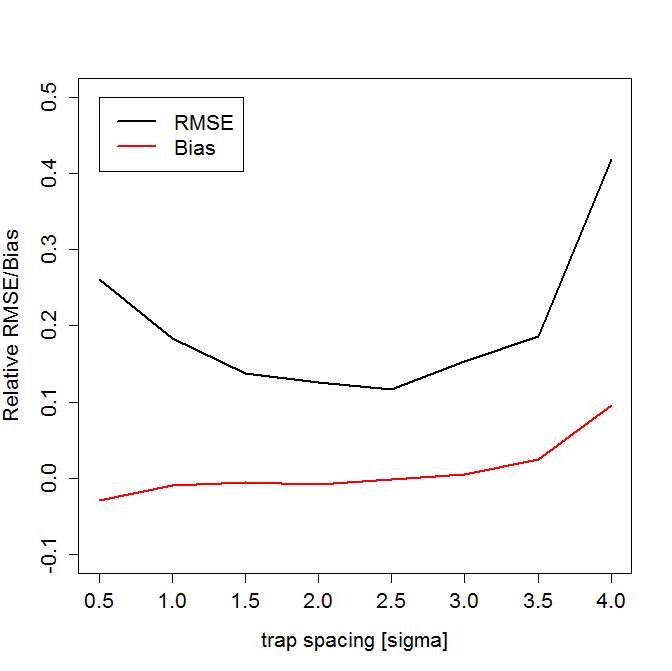
\includegraphics[width=3in]{Ch10-Design/figs/RMSE.png}
\caption{Fort Drum Black bear study area and the 38 baited hair snare
  locations operated for 8 weeks during June and July, 2006.}
\label{design.fig.rmse}
\end{figure}



% In summary, SCR models performed best when $\sigma^*$ was slightly
% larger than trap spacing (or in other words, when $\sigma$ was
% slightly smaller) and did well as long as $\sigma^*$ was at least 0.5
% times the average distance between traps (which corresponds to
% $\sigma$ being 0.35 times the average distance between
% traps). Although at this trap spacing to movement ratio, most
% individuals are captured at one trap only (see
% Tab. \ref{design.tab.simdat}), parameter estimates exhibited low bias
% and remained relatively precise (see simulation results for $\sigma^*$
% = 1 in Tab. \ref{design.tab.simres}). Below this trap spacing to
% movement ratio the spatial information in the simulated data
% apparently was not sufficient to inform SCR model parameters.


\subsection{Example: Black bears from Pictured Rocks National Lakeshore }

To see how trap array size influences parameter estimates from spatial
capture-recapture models in the real world, \citet{sollmann_etal:2012}
also looked at a black bear data set from Pictured Rocks National
Lakeshore, Michigan, collected using 123 hair snares distributed over
an area of 440 $km^2$ along the shore of Lake Superior in May-July
2005 \citep{belant_etal:2005}.  The SCR model for the bear data
included sex-specific
encounter rate parameters, and an occasion-specific baseline encounter
rate.
%and
%$\sigma^*$ between males and females, and $\lambda_0$ varied across
%occasions.
This was motivated by a) the lower average number of
detections for male bears, b) the decreasing number of detections
over time in the raw data, and c) the fact that male black bears are
known to move over larger areas than females (e.g.,
\citealp{gardner_etal:2010jwm, koehler_pierce:2003}).

To address the impact of a smaller trap array on the parameter
estimates, models fitted to the full data set were compared to
models fitted to data subsets.
The first subset retained only those 50\% of the traps
closest to the grid center. In the second, only the southern 20\% of
the traps were retained \ref{design.tab.bears}.

\begin{table}[ht]
  \centering
  \caption{Posterior summaries of SCR model parameters for black
    bears, modified from \citet{sollmann_etal:2012}.}
    \begin{tabular}{lcccc}
%    \addlinespace
	\hline
          & Mean (SE) & Mode  & 2.5\% & 97.5\% \\ \hline
    {\bf Full data set} &       &       &       &       \\
    {\it D } & 10.556 (1.076) & 10.448 & 8.594 & 12.792 \\
    $\sigma^*$ (males) & 7.451 (0.496) & 7.323 & 6.579 & 8.495 \\
    $\sigma^*$ (females) & 2.935 (0.143) & 2.939 & 2.671 & 3.226 \\
    {\bf 50\% of traps} &       &       &       &      \\
    {\it D } & 12.648 (1.838) & 12.205 & 9.307 & 16.713 \\
    $\sigma^*$ (males)  & 5.354 (0.511) & 5.248 & 4.472 & 6.473  \\
    $\sigma^*$ (females) & 3.318  (0.277) & 3.262 & 2.841 & 3.910 \\
    {\bf 20\% of traps} &       &       &       &        \\
    {\it D } & 6.752 (1.611) & 5.953 & 4.000 & 10.218  \\
    $\sigma^*$(males)  & 9.881 (3.572) & 7.566 & 5.121 & 18.447 \\
    $\sigma^*$ (females)  & 2.686 (0.391) & 2.657 & 2.121 & 3.404  \\
    \hline
    \end{tabular}
  \label{design.tab.bears}
\end{table}

Reducing the area of the trap array by 50\% created a grid polygon of
144 $km^2$, which was smaller than an estimated male black bear home
range and only 50\% larger than a female black bear home range --
approximately 260 $km^2$ and 100 $km^2$, respectively, when converting
estimates of $\sigma^*$ to home range size. Table
\ref{design.tab.bears} shows that this did not greatly influence model
results, compared to the full data set. The observed smaller
differences in parameter estimates may be due to individual
differences in detection and movement that manifest themselves when
only a smaller portion of the overall population is sampled. By
reducing the number of traps we effectively reduced the size of the
overall data set estimates were based on (both in terms of individuals
captured and recaptures).
% XXXX RBC says: the previous 2 sentences were not so clear.
This was reflected in overall higher SE and
wider confidence intervals. In spite of these differences, density
estimates %-\226 the main objective of applying SCR models -�
%remained largely constant.
were similar.
Removing 80\% of the traps and thereby % XXXX begin new paragraph?
reducing the area of the trap array to 64 $km^2$ -- well below the
average black bear home range -- had a great effect on sample size
(only 25 of the original 83 individuals sampled) and parameter
estimates. Particularly, male black bear movement was overestimated
and imprecise. The combination of the low baseline trap encounter rate
of males and the considerable reduction in sample size led to a low
level of information on male movement: 5 of the 12 males were captured
at one trap only. Although they moved over smaller areas, owing to
their higher trap encounter rate females were, on average, captured at
more traps (3.4 traps per individual compared to 2.6 for males) so
that their movement estimate remained relatively
accurate. Overestimated male movements and female trap encounter rates
resulted in an underestimate of density of almost 40\%. This effect
is contrary to what we would expect to see in non-spatial CR models,
where too small an area % XXXX RBC says: this isn't so clear. Do you
                        % mean, using an ad hoc value of effective
                        % sample area that is too small?
leads to underestimated movement and
overestimated density \citep{bondrup-nielsen:1983, dillon_kelly:2007,
  maffei_noss:2008}. While this example again demonstrates the ability
of SCR models to deal with a range of trapping grid sizes, it also
clearly shows that your study design needs to consider the amount of
data you can expect to collect.

\subsection{Summary thoughts on trap spacing and array size in SCR models}
% XXXX RBC says: In what way is this "final"?
%XXX Andy: I changed the heading but that doesn't resolve the problem
% XXX Maybe we need to rethink the intent of this subsection

When designing a capture-recapture study for a single species, trap
spacing and the size of the array can (and should) be tailored to the
spatial behavior of that species to ensure adequate data
collection. However, some trapping devices like camera traps may
collect data on more than one species and researchers may want to
analyze these data, too. Independent of the trapping device used,
study design will in most cases face a limit in terms of the number of
traps available or logistically manageable. As a consequence,
researchers need to find the best compromise between trap spacing and
the overall grid area. In the following sections we consider both
practical approaches to this trade-off and a model-based approach to
derive such an optimal study design.

Particularly for large mammal research, SCR models have much more
realistic requirements in terms of area coverage than non-spatial CR
models, under which density estimates can be largely inflated with
small trapping grids relative to individual movement
\citep{maffei_noss:2008}.
% XXXX RBC says: I agree with this previous sentence, but I'm not sure
% tha tthe reader fully understands why this is so, at this point.
How large the spatial survey effort needs to
be does not only depend on the extent of movement of the target
species, but also on the temporal effort, density and detection
probability \citep{marques_etal:2011} -- in summary, the amount of
data that can be collected with any given trap array. For low-density
species, like the black bears in the above example, small trapping
grids bear % XXXX No pun intended!?
the risk of not collecting enough data for parameter
estimation. Simulation studies can help you assess how effective a
certain study design is given a set of parameters. Alternatively,
\citet{efford_etal:2009ecol} provide a mathematical procedure to
determine the expected number of individuals captured and recaptures
for a given detector array and set of model parameters.
% XXXX Perhaphs efford_etal:2009ecol should have been mentioned earlier

% XXXX RBC says: This paragraph seems pretty redundant with previous material
Overall, while there are limits to the flexibility in spatial trap
array design for SCR modeling, the method is fairly robust to changes
in trap array size and spacing relative to animal movement. Trapping
grids with an extent of approximately a home range diameter can, %�
in theory, %-
adequately estimate density and home range size. However,
these results should not encourage researchers to design non-invasive
trap arrays based on minimum area and spacing requirements. Study
design should still strive to expose as many individuals as possible
to sampling and obtain adequate data on individual movement. Large
amounts of data do not only improve precision of parameter estimates
(the density estimate for the full black bear data set has narrower
confidence intervals than estimates from the reduced data sets), they
also allow including potentially important covariates (such as gender
or time effects in the black bear example) into SCR models to obtain
density estimates that reflect the actual state of the studied
population.



\section{Sampling Over Large Areas}

Trap spacing is an essential aspect of design of SCR studies. However,
it is only the most important aspect if one can uniformly cover a
study area with traps.   In many practical situations where the study
area is large relative to effort that can be expended, one has to
consider other strategies which deviate from a strict focus on trap
spacing. There are two general strategies that have been suggested
which we think are useful in practice, either by themselves or
combined: Sampling based on {\it clusters} of traps and sampling based
on {\it rotating} groups of traps over the landscape.

\citet{karanth_nichols:2002} describe 3 approaches of moving traps to
achieve coverage of a larger study area, geared towards traditional
capture-recapture analysis. Say, to sample the entire area of interest
requires sampling $J$ sites.

{\flushleft \bf (1)} For every day/sampling occasion, randomly choose
$x$ out of your $J$ sites, where $x$ is the number of trapping devices
you have at hand. Obviously, this requires the logistics of moving
traps to be quite easy.  \newline
{\flushleft \bf (2)} Move blocks of traps
that are close to each other in space daily. For example, if you
divide your total study area into 4 blocks, sample block 1 for a day,
then move traps to block 2 for a day, and so forth, and repeat until
each block has been sampled for a sufficient amount of time. \newline
{\flushleft \bf (3)} If moving blocks of traps daily is too
challenging, logistically, then you can sample each block for a
certain number of days/occasions before moving cameras to the next
block. In this fashion, you only need to move traps to each block
once.

In traditional CR we collapse data across traps and assume all
individuals in the study area have some probability $>0$ of being
detected. For our data that means that, under scenario (2) the first
occasion is defined as the time it takes to sample all 4 blocks once,
the second occasion consists of the second round of sampling all
blocks, etc. Under scenario (3), we have to combine data from day 1 in
each of the blocks to form occasion 1, data from day 2 in each of the
blocks forms occasion 2, and so on. Especially scenario 3 makes
modeling time-dependent detection difficult, since occasion 1 does no
longer refer to an actual day or continuous time interval.
We do not have that problem in SCR, where accounting for trap site
specific sampling effort is straight forward, as we first demonstrated
for the wolverine example in Sec. \ref{scr0.sec.wolverine}. Because we
are dealing with detection at the trap level, even for design (3) in a
spatial framework, we can still look at variation in detection over
time. As such, we don't think that one of the above designs is
superior for SCR models than the other, but rather, all of them will
produce adequate SCR data, as long as overall sample size requirements
are met.

\citet{efford_fewster:2012} looked at the performance of different
spatial study designs for abundance estimation from traditional and
spatial capture-recapture models, including a clustered design, where
groups of detectors are spaced throughout the larger region of
interest. They found that this design performed well, although there
were indications of a slight positive bias in estimates of $N$. Such a
clustered design enables researchers to increase area coverage without
having to increase the number of traps. \citet{efford_fewster:2012}
note that distribution of clusters has to be spatially representative
-- for example, systematic with a random origin. 
\citet{efford_etal:2009ecol} suggest a clustered type of design for
acoustic detectors (see Chapt. \ref{poisson-mn.sec.acoustic}, suggesting a design comprised of multiple small
(e.g., $2 \times 2$) clusters distributed in a probabilistic fashion
across the region of interest.
The issue of
spatially representative designs is not limited to SCR and an
extensive treatment of the topic can be found in the distance sampling
literature \citep{buckland_etal:2001}. Further, the authors stress
that, if distances among clusters are large and individuals are
unlikely to show up in several clusters, then the method relies on
spatial recaptures {\emph within} clusters, meaning that spacing of
detectors within clusters has to be appropriate to the movements of
the species under study.

In practice, employing both of these strategies -- clustering and
rotating traps -- might be necessary or advantageous. Especially for
clustered designs, further research on optimal detector configurations
is called for \citep{efford_fewster:2012}. More generally, work on
formalizing and generalizing these ideas of spatial study design is
needed.  We believe the model-based spatial design approach, which we
introduce below, is the way to do that.


\citet{sun:2013} used a simulation study to investigate different trap
arrangements (Fig. \ref{design.fig.sun}) for a black bear study based
on hair snares distributed over 2625 km$^2$ study area. She simulated
populations of bears for 3 trap arrangements including a regular
(uniform) coverage of traps, clusters of size 4 traps each with a gap
between clusters, and a design in which the clusters of size 4 were
moved mid-way through the study to fill the gap (we'll call this a
``rotating'' design).  She found that the precision and accuracy of of
$N$ estimates generally decreased when changing from uniform to
cluster to rotating design.


\begin{figure}[ht]
\centering
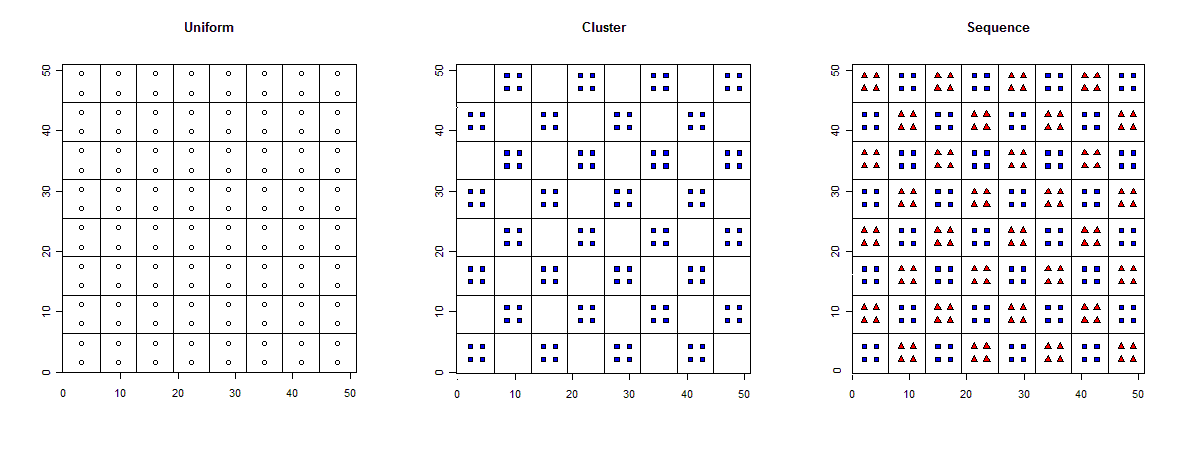
\includegraphics[width=5in,height=1.94in]{Ch10-Design/figs/catsun_designs.png}
\caption{Three designs evaluated by Sun XXXXX.  }
\label{design.fig.sun}
\end{figure}





\section{Model-Based Spatial Design}

A point we have stressed in previous chapters is that SCR models are
basically glorified versions of generalized linear models (GLMs) with
a random effect that represents a latent spatial attribute of
individuals, the activity center or home
range center.  This formulation makes analysis of the models readily
accessible in freely available software and also allows us to adapt
and use concepts from this broad class of models to solve problems in
spatial capture recapture. In particular, we can exploit
well-established model-based design concepts 
\citep{kiefer:1959,
box_draper:1959,
box_draper:1987,
fedorov:1972,
sacks_etal:1989,
hardin_sloane:1993,
fedorov_hackl:1997}
to develop a framework for designing
spatial trapping arrays for capture-recapture studies.
\citet{muller:2007} provides a recent monograph level treatment of the subject
that is very accessible.

In the following sections, we adapt these classical methods for
constructing optimal designs to obtain the configuration of traps (or
sampling devices) in some region (the design space, ${\cal X}$), that
minimizes some appropriate objective function based on a compromise
between the variance of estimating $N$ for a prescribed
state-space. We show that this criterion -- based on the variance of
an estimator of $N$ -- represents a formal compromise between
minimizing the variance of the MLEs of the detection model parameters
and obtaining a {\it high} expected probability of capture.
Intuitively, if our only objective was to minimize the variance of
parameter estimates than all of our traps should be in one or a small
number of clusters where we can recapture a small number of
individuals many times each. Conversely, if our objective was only to
maximize the expected probability of encounter then the array should
be highly uniform so as to maximize the number of individuals being
exposed to capture.  By seeking to minimize the variance of of an
estimator of $N$, our objective function is, formally, a compromise
between these two objectives and the resulting designs are not always
highly regular nor clustered.

% Existing theory (Sanathanan 1972) suggests that such designs
%should also be optimal for estimating density or abundance.

\subsection{Formalization of the Design Problem for SCR Studies}

Let ${\cal X}$, the {\it design space}, denote some region within
which sampling could occur and let ${\bf X} = {\bf x}_{1},\ldots, {\bf
  x}_{J}$ denote the {\it design}, the set of sample locations (e.g.,
of camera traps), normally we just call these ``traps.''  The design
space ${\cal X}$ must be prescribed (a priori).  Operationally, we
could equate ${\cal X}$ to the study area itself (which is of
management interest) but, in practical cases, there will be parts of
the study area that we cannot sample. Those areas need to be excluded
from ${\cal X}$.  While ${\cal X}$ may be continuous, in practice it
will be sufficient to represent ${\cal X}$ by a discrete collection of
points which is what we do here.  This is especially convenient when
the geometry of ${\cal X}$ is complicated and irregular, which would
be the case in most practical applications).  The technical problem
addressed subsequently is how do we choose the locations ${\bf X}$ in
a manner that is statistically efficient for estimating abundance or
density, or perhaps some other variance-based criterion?

As usual, we regard the population of $N$ such individual ``activity
centers'' as the outcome of a point process distributed independently
over the state-space ${\cal S}$.  The relevance and importance of
${\cal S}$ has been established repeatedly in this book, as it 
defines a population of individuals (i.e., activity
centers) and, in practice, it is not usually the same as ${\cal X}$
due to the fact that animals move freely over the landscape and the
location of traps is typically restricted by policies, ownership and
other considerations.  The objective we pursue here is: Given (1)
${\cal X}$, (2) a number of design points, $J$; (3) the state-space
${\cal S}$, and (4) an SCR model, and (5) a design criterion $Q({\bf
  X})$, we want to choose {\it which} $J$ design points we should
select in order to obtain the {\it optimal} design under the chosen
model, where the optimality is with respect to $Q({\bf X})$. We will
describe some possible choices for $Q({\bf X})$ below, but it makes
sense that they should relate to the variance of estimators of one or
more parameters of the SCR model.

To motivate the approach we're going to take in a simplified situation,
suppose for the moment that we know ${\bf
  s}$ for a single  individual.  In this case, its vector of counts of
encounter in each trap ${\bf y}$ are either binomial or Poisson
counts, and the model has this form:
\begin{equation}
g( \mathbb{E}({\bf y})  ) =  \alpha_0  + \alpha_1 ||{\bf x}-{\bf s}||^2.
\label{eq.linearpredictor}
\end{equation}
Or based on some other encounter probability model. In vector form we
write this as:
\[
g( \mathbb{E}({\bf y})  ) =  {\bf M}'{\bm \alpha}
\]
where ${\bf M}$ is the $J \times 2$ design matrix where the 2nd column
contains the squared pairwise distances between each individual $i$
and trap $j$, and thus it depends on both ${\bf X}$ and ${\bf s}$.  A
simpler model is the normal linear model, of the form:
\[
{\bf y} = {\bf M}({\bf X},{\bf s})'{\bm \alpha} + \mbox{error}
\]
The variance-covariance matrix of $\hat{\bm \alpha}$ is, supressing
the dependence on ${\bf X}$, 
\[
 \mbox{Var}( {\bm \alpha},{\bf X}) = ({\bm M}({\bf s})'{\bm M}({\bf s}))^{-1}
\]
Note that the design points ${\bf x}_{j}$ appear explicitly (in the
2nd column of {\bf M}).  In considering design for estimation in such
models it is natural to choose design points, corresponding to values
of ${\bf x}$, such that the variance of $\hat{\bm \alpha}$ is
minimized.  In particular, for a population of $N$ individuals, if we
know {\it all} $N$ values of ${\bf s}$ we could now easily find the
design ${\bf X}$ that optimizes some function of the
variance-covariance matrix, whatever function we want.  If we don't
know ${\bf s}$ then we might consider minimizing  the expected variance:
\[
  E_{{\bf s}}\left\{ \mbox{Var}({\bm \alpha},{\bf X}) \right\} = \sum_{s \in
    {\cal S}}  ({\bf M}'({\bf s}){\bf M}({\bf s}))^{-1}
\]
but this is not the expected variance based on sampling a population of $N$
individuals, just for a single individual having unknown ${\bf
  s}$. Because of the matrix inverse in this expression, it is not
sufficient to use a variance criterian that weights this variance by
$N$ or even the expected sample size. 
As an alternative, 
we can maximize the expected {\it information} which is probably more
appealing from an analytic point of view.
The information matrix is:
\[
 \mbox{Inf}({\bm \alpha},{\bf X}) = 
 ({\bf M}'({\bf s}){\bf M}({\bf s}))
\]
and, for a population of individuals, let ${\bf M}_{i}$ be the design
matrix for individual with 
activity center ${\bf s}_{i}$, the total information is:
\[
 \mbox{Inf}({\bm \alpha},{\bf M}_{1},\ldots,{\bf M}_{N}) = 
 \sum_{i=1}^{N}  ({\bf M}_{i}'({\bf s}_{i}){\bf M}_{i}({\bf s}_{i}))
\]
Now, because we don't know ${\bf s}_{i}$ we can compute the integrated
information, over all possible values of ${\bf s}_{i}$, and for {\it
  each} ${\bf s}_{i}$, which is an $N$-fold summation:
\[
E_{ {\bf s}_{1}, \ldots, {\bf s}_{N}}
\left\{  \mbox{Inf}({\bm \alpha},{\bf M}_{1},\ldots,{\bf M}_{N}) \right\} = 
 \sum_{i=1}^{N}  \sum_{s \in {\cal S}} ({\bf M}_{i}'({\bf s}_{i}){\bf M}_{i}({\bf s}_{i}))
\]
which, if the activity centers are independent, is just $N$ copies of
the integrated (spatially averaged) information:
\[
E_{ {\bf s}_{1}, \ldots, {\bf s}_{N}}
\left\{  \mbox{Inf}({\bm \alpha},{\bf M}_{1},\ldots,{\bf M}_{N}) \right\} = 
N  \sum_{s \in {\cal S}} ({\bf M}_{i}'({\bf s}_{i}){\bf M}_{i}({\bf s}_{i})).
\]

It therefore seems sensible to 
 base design of SCR studies on some criterion that is a
function of this  integrated information matrix. E.g., maximize the diagonals, or the determinant.
This can be done for any number of design points ${\bf x}_{1},\ldots,
{\bf x}_{J}$ using standard exchange algorithms
\citep[see][Chapt. 3]{muller:1997} and we discuss this below
in Sec. \ref{design.sec.exchange}.
%which always improve the criterion but will not necessarily yield {\it
%  the} optimal design. 

It is worth noting that asymptotic formulae for
$\mbox{Var}( {\bm \alpha})$ can be cooked up for any type of GLM.
For the Poisson GLM, the asymptotic
variance-covariance matrix of $\hat{\bm \alpha}$, considering a single
individual having location ${\bf s}$, is\footnote{ e.g., see
  some appendix in the back of McCullogh and Nelder XXXXX or Agresti XXXX for
  example -- this is basic GLM theory that derives from the fact that
  the Poisson is a member of the natural exponential family of
  distributions.}
\begin{equation}
  \mbox{Var}(\hat{\bm \beta}|{\bf X},{\bf s}) 
=  ({\bf M}({\bf s})' {\bf D}({\bm \beta},{\bf s}){\bf M}({\bf s}))^{-1}.
\label{eq.varbeta}
\end{equation}
This is a 
 function of the design ${\bf X}$ as well as ${\bf s}$ both of which
 are balled-up in ${\bf M}$ --
the regression design matrix, and the matrix ${\bf D}$ which is a diagonal
matrix having elements $\mbox{Var}( y_{j}|{\bf s}) = \exp({\bf
  m}'{\bm \beta})$ for $y_{j}$ the frequency of encounter in trap $j$.

To summarize the main point: If we know where the guys live, we can
pick he optimal design directly. But we don't! So what do we do?




\subsection{An Optimal Design Criterion for SCR}

There are a number of appealing directions to pursue for deriving a
variance-based criterion upon which to devise designs for capture
recapture studies.  For one, we could formulate the problem as a
Huggins-Alho type of problem and follow along their analysis for
computing variances, and that might be fruitful. But the calculus is
a bit tedious for that.  Instead, a more fruitful area is to consider
the MLEs based on the marginal  Poisson or Binomial likelihoods, and then we
could possibly compute the variance-covariance matrix of the MLEs
directly.  This merits further investigation.   We take an easier
approach here, for illustrative purposes, devising 
a variance criteria based on
a conditional estimator of $N$ of the form
\[
  \tilde{N}  =  \frac{n}{\bar{p}}
\]
where $\bar{p}$ is the probability that an individual appears in the
sample of $n$ unique individuals. In SCR models an individual with activity center
${\bf s}_{i}$ is captured if it is
captured in {\it any} trap and therefore, under the Bernoulli model,
\[
 \bar{p}({\bf s}_{i}, {\bf X}) = 1 - \prod_{j=1}^{J} (1- p_{ij}({\bf
   x}_{j}, {\bf s}_{i}))
\]
and, under the Poisson model, we have:
\[
 \bar{p}({\bf s}_{i},{\bf X}) = 1 -  \exp(-\lambda_{0} \sum_{j}
 \exp(\beta* d({\bf x}_{j}, {\bf s}_{i})^2 ))
\]
where here we emphasized that this is conditional on ${\bf s}_{i}$ and
also the design -- the trap locations ${\bf x}_{j}$.
 The {\it
  marginal} probability of encounter, averaging over all possible
locations of ${\bf s}$ is:
\begin{equation}
 \bar{p}({\bf X}) = 1 - \int_{\bf s}    \bar{p}({\bf s}_{i},{\bf X})    d{\bf s}.
\label{design.eq.pbar}
\end{equation}
It is important to note that this can be calculated directly {\it
  given} the design ${\bf X}$. This is handy because we see that it is
used in the variance formulae given subsequently.

The approach we take here is we develop the variance of $\tilde{N}$
conditional on knowing the locations of all $N$ individuals and then
we suggest to unconditon on the realized point process by taking a
Monte Carlo average over realizations of ${\bf s}$ under a suitable
model for ${\bf s}$. The variance criterion we propose here is based
on a delta approximation $Var(n/\bar{p})$:
\begin{equation}
 Var(\tilde{N}(\bm \alpha) ) =
\frac{N^{2} Var(\bar{p})}{\bar{p}^{2}}  + N\frac{(1-\bar{p})}{\bar{p}}
\label{design.eq.theQ}
\end{equation}
This is a really intuitive-looking criterion upon which to base
designs. In particular, it is the sum of two components
which are
essentially those due to (1) estimation of $\bar{p}$ from the sample
and (2) the variance of $n$. We see that generally this criterion is improved
(decreases) as we do a better job estimating $\bar{p}$ and also as $n$
approaches $N$, i.e., as $\bar{p}$ increases to 1. Thus, good designs
should generate information about detection probability {\it and}
produce large samples of individuals.  The other way to look at this
is that the variance of estimating $N$ is due to the variance of
estimating $\bar{p}$ with a {\it penalty} due to have a low value of
$\bar{p}$ (the 2nd term being the penalty, which increases as
$\bar{p}$ goes to 0).  We suggest, therefore, that designs for
capture-recapture studies should seek to minimize
Eq. \ref{design.eq.theQ}, or perhaps generalizations of this to
account for other features of the model.



In order to work with this expersssion we will
have to do some analysis of $\mbox{Var}(\bar{p})$ which we take up now.
We note that $\bar{p}$ is itself a deterministic function of the
parameters that we need to estimate, ${\bm \alpha}$. Therefore, as a
general rule,  we could use
a delta approximation to  express $\mbox{Var}(\bar{p})$ in terms of the variance of
the MLE $\hat{\bm \alpha}$.  However, we stated above that our intent
is to work with the Poisson observation model, and we did that because
the technical argument that follows is somewhat easier for that
case. In particular, we first express the integral in Eq.
\ref{design.eq.pbar} by a summation over a fine mesh of points so that:
\[
 \bar{p}({\bf X}) = \sum_{{\bf s}} 1 -    \bar{p}({\bf s}_{i},{\bf X})
\]
which under the Poisson model is, in a simplified notation:
\[
 \bar{p}({\bf X}) = \sum_{{\bf s}} \left\{
1 -  \exp(-\lambda_{0} \sum_{j}
 exp(\beta* d({\bf x}_{j}, {\bf s})^2))
\right\}
\]
To compute the variance of this expression, we note that the variance
operature can move inside the summation over ${\bf s}$, and the
subtraction from 1 doesn't count anything, so we have
\[
Var( \bar{p}({\bf X}) )  = \sum_{{\bf s}}
 Var \left(
 \exp(-     \sum_{j}   exp(\alpha_{0} + \alpha_{1}  d({\bf x}_{j}, {\bf s})^2))
   \right)
\]
At this point we apply the Delta approximation to produce
\[
Var( \bar{p}({\bf X}) )  = \sum_{{\bf s}}
\left( exp( - \sum_{j} exp(\alpha_{0} + \alpha_{1}  d({\bf x}_{j}, {\bf  s})^2) )
\right)
 Var \left(    \sum_{j}   exp(\alpha_{0} + \alpha_{1}  d({\bf x}_{j}, {\bf     s})^2)    \right)
\]
we're going to simplify things a bit and write $\lambda({\bf
  x}_{j},{\bf s}) =   exp(\alpha_{0} + \alpha_{1}  d({\bf x}_{j}, {\bf
  s})^2)$
and also $\lambda_{\bf s} = \sum_{j=1}^{J} \lambda({\bf x}_{j},{\bf
  s})$. Then
\[
Var( \bar{p}({\bf X}) )  = \sum_{{\bf s}}
\left( exp( - \lambda_{\bf s} )  \right)
 Var \left(    \sum_{j}   exp(\alpha_{0} + \alpha_{1}  d({\bf x}_{j}, {\bf     s})^2)    \right)
\]
We have to do a 2nd application of the Delta approximation to find
that:
\[
Var( \bar{p}({\bf X}) )  =
\sum_{{\bf s}} \left( exp( - \lambda_{\bf s} )  \right)
\left(    \sum_{j}  \lambda({\bf x}_{j},{\bf s})^{2} Var( \hat{\alpha}_{0} + \hat{\alpha}_{1}  d({\bf x}_{j}, {\bf    s})^2)
  \right)
\]
(note: need to comment on why $\alpha$ has hats on it somewhere but
not elsewhere)
The final step is we assume $\hat{\alpha}_{0}$ and $\hat{\alpha}_{1}$
are independent which is not true in practice but makes life slightly
easier here (but is not necessary, in general). The variance of
$\bar{p}$ becomes:
\[
Var( \bar{p}({\bf X}) )  =
\sum_{{\bf s}} \left( exp( - \lambda_{\bf s} )  \right)
\left(    \sum_{j}  \lambda({\bf x}_{j},{\bf s})^{2} (
 Var( \hat{\alpha}_{0}) +
  d({\bf x}_{j}, {\bf    s})^4
Var( \hat{\alpha}_{1})  )
  \right)
\]



The big picture is this: For a given design ${\bf X}$, we can compute
the $\mbox{Var}(\bar{p}({\bf X}))$ -- its just a calculation involving sum's
over all points in the state-space and design points -- provided we
know the variance of the estimator of ${\bm \alpha}$,
$Var(\hat{\bm \alpha})$.
However, it is not so easy to write down the analytic form of this matrix.
 Some calculus would have to be done on the
conditional likelihood (e.g., from \citet{borchers_efford:2008}) to figure
out the asymptotic form of this matrix.  For our purposes,  a good heuristic is
to approximate the matrix, using the analogous result from a Poisson or Binomial GLM assuming
that $N$ is known,
since we have conveneint formulas for those.  In particular, if we knew the
activity centers of all individuals then the resulting data $y(x,s)$
are Poisson counts. The asymptotic variance-covariance matrix of ${\bm
  \alpha}$ in that case is:
\begin{equation}
  \mbox{Var}(\hat{\bm \alpha}|{\bf X},{\bf s})
=  ({\bf M}({\bf s})' {\bf D}({\bm \alpha},{\bf s}){\bf M}({\bf s}))^{-1}.
\label{eq.varbeta}
\end{equation}
where ${\bf M}$ is a matrix which has a column of 1's and a column of
$N \times J$ entries that are the distances between each individual
and each trap and the matrix ${\bf D}$ is a diagonal matrix having
elements $\mbox{Var}( y_{j}|{\bf s}) = exp({\bf m}'{\bm \alpha})$ for
$y_{ij}$ the frequency of encounter in trap $j$.  Thus, the variance
is a function of the design ${\bf X}$ as well as ${\bf s}$ both of
which are balled-up in ${\bf M}$ -- the regression design matrix and
the matrix ${\bf D}$.

This is conditional on ${\bf s}$...... what do we do?  Well , we look
at it this way: What is the {\it expected} information obtained from a
particular realization of $N$ individuals?  Clearly that should be:
\[
I(N) =  M_{1}' D_{1} M_{1} + .... M_{N}D_{N} M_{N}
\]
so we can average this over all possible collections of $N$ values of
${\bf s}$. clearly, if {\it individual activity centers are
  independent}
 this is exactly the same as taking a single MC
average over {\it all} elements of the state-space weighted by $N$:
\[
E[{\bf I} ] = N  \sum_{{\bf s}}  M({\bf s})'D({\bf s}) M({\bf s})
\]





Therefore we have a design criterion which is obtained by plugging
$\bar{p}$ from Eq. XXXX {\it and} the variance expression
xxxx   nto Eq. \ref{design.eq.theQ}.
 This is a function of the design ${\bf  X}$ and also the ballpark
 guess of the model parameters................





\subsection{Optimization of the criterion}
\label{design.sec.exchange}

To build spatial designs that optimize the criterion,
we need to come up with a ballpark guess of the model
parameters so that the criterion can be evaluated. i.e., what are ${\bm
  \alpha}$ and $N$? If we do that, and specify
the state-space ${\cal S}$ then, we can, in
theory, optimize the variance criterion over all possible
configurations of $J$ traps.

In formulating the optimization problem note that we have $J$ sample
locations corresponding to rows of ${\bf X}$.  The problem is a $2J$
dimensional optimization problem which, for $J$ small, could be solved
using standard numerical optimization algorithms as exist in almost
every statistical computation environment.  However, $J$ will almost
always be large enough so as to preclude effective use of such
algorithms. This is a common problem in experimental design, design
for response surface estimation, computer experiments, spatial
sampling designs and other disciplines for which sequential exchange
or swapping algorithms can be used \citep[e.g.,][]{wynn:1970,
fedorov:1972, mitchell:1974, meyer_nachtsheim:1995}.
 The basic idea is to pose the problem as a sequence
of 1-dimensional optimization problems in which the objective function
is optimized over 1 or several coordinates at a time.
In the present case, we consider swapping out ${\bf x}_{j}$ for some
point in ${\cal X}$ that is nearby ${\bf x}_{j}$ (e.g., a 1st order
neighbor). The objective function is evaluated for all possible swaps
(at most 4 in the case of 1st order neighbors) and whichever point
yields the biggest improvement is swapped for the current value.  The
algorithm is iterated over all $J$ design points and this continues
until convergence is achieved. Such algorithms may yield local optima
and optimization for a number of random initial designs can yield
incremental improvements. We implemented this swapping algorithm in
{\bf R}, using the basic strategy employed elsewhere (e.g., Nychka et
al. 1997; Royle and Nychka 1998).  A version of a swapping
algorithm used to optimize a space-filling criterion is implemented
in the {\bf R} package {\bf
  fields} (Fields Development Team 2006).  We developed an
  implementation that operates on
a discrete representation of ${\cal S}$ (an aribtrary matrix of
coordinates).
For each point in ${\bf X}$, only
the nearest neighbors (the number is specified) are considered for
swapping into the design during each iteration.

While swapping algorithms are convenient to implement, and efficient
at reducing the criterion in very high dimensional problems, they do
not always yield the global optimum.  In practice, as in the examples
below, it is advisable to apply the algorithm to a large number of
random starting designs.  Our experience is that essentially
meaningless improvements are realized after searching through a few
dozen random starts.



\subsection{Illustration}

Because the algorithm operates on a discrete version of ${\cal S}$,
it is trivial to apply to situations in which the
state-space is arbitrary in extent and geometry. However, we consider
a simplified situation here in order to illustrate the calculation of
optimal designs and how they look for an intuitive situation.


Consider designing a study for camera traps in a square region defined
by the square $[10,20] \times [10, 20]$ and with ${\cal X} = {\cal
  S}$.  For this illustration I assumed $\beta_{0} = log(\lambda_{0})
= -2.7$ and $\beta_{1} = 1/(\sigma^{2}) = 1/4$, $1/9$ and $1/16$, so
$\sigma = 2,3,4$. (this was dumb - note that $\sigma$ is really 2
times the standard deviation of a normal distribution. Oh well!).
Designs of size 9 and 10 were computed for each value of $\sigma$
using many random starting designs.  The putative optimal designs
(henceforth ``best'') are shown\footnote{My intention is to provide
  many of these results in an Appendix in order to reduce the length
  of the paper.} in Figure \ref{fig.fig1}.  For J=9, $\sigma =2$, the
best design was produced in 180 out of 1000 random starts.  For
$\sigma = 3$ (row 2, left panel) the best design was produced in about
88\% of all optimizations from random starting values.
%reason is that there are a lot of points in the interior that interact
%relatively little with the design and these ``holes'' tend to cause
%the algorithm to get caught in a local optimum (my interpretation) of
%the objective function.  Or, consider this, with sigma = small the
%design can probably be translated a little bit in space .... this is
%what I think happens.
For $J=10$, and $\sigma =2$ (row 1, right panel), the best design was
found about 24\% of the time (from random starts).
The $\sigma = 3$ best design (row 2, right
panel; 14\% of random starts) clusters 2 points in the center.
Finally, consider the $\sigma =4$ case (last row of
Fig. \ref{fig.fig1}).  We have two irregular looking designs and
the design points cluster in various ways.
% For $J=9$ this was produced
%only 1 time whereas only 8 instances of 1000 produced the
%best design for $J=10$.  We might thus have little confidence in that
%result\footnote{subsequent analyses have failed to find a better
%  design.}.

I computed the best designs using the same settings but inreasing the
size of ${\cal S}$ relative to ${\cal X}$.  In particular, I nested
${\cal X}$ into $[9,21] \times [9,21]$ (Figure \ref{fig.fig2})
 and then $[8,22]^{2}$ (Figure \ref{fig.fig3}).
The obvious effect of this is
that the best designs move points toward the edge of the design space
${\cal X}$ so as to provide more exposure to points in ${\cal S}$.
The effect is more pronounced, obviously, as you provide more area
outside of ${\cal X}$ that is allowed to influence the design.

As a final example,
consider placing 20 camera traps in this region. Where do they
go? Look at the 3 buffers, 3 values of sigma, thats 9 total designs
(use a single panel).
An interesting feature of the designs is that they are not
regular. Traps occur in clusters of several traps close together
with the clusters more widely spaced.



\subsection{Density covariate models}

Many capture-recapture studies will involve one or more landscape or
habitat covariates that are thought to affect density, with the idea
of using the methods described in Chapt. \ref{chapt.state-space} for
modeling and inference.  We imagine that it should be possible to
extend the model-based framework described previously to accomodate
uncertainty due to having to estimate ${\bm \beta}$, and this could be
included as a feature of the design criterion.

In this case, we can think
of the captures in a trap being Poisson random variables with mean
$\lambda({\bf x},{\bf s})*D({\bf s})$ and we think the same arguments
as given above can be used to devise design criteria and optimzie
them. However, in this case we might not only care about estimating
$N$ but also (or instead) inference about the parameters ${\bm
  \beta}$. Thus, we might choose designs that are good for $N$ or
perhaps only good for estimating ${\bm \beta}$ or perhaps both.
Intutively, we think these two design objectives conflict with one
another to some extent.  Model-based approaches should favor areas of
higher density, but the design pionts need to realize variation in the
landscape covariates too.



\section{Temporal aspects of study design}

The spatial configuration of traps is one of the most important
aspects of sampling design for capture-recapture studies. Indeed, as
we discussed in the previous section, design under SCR models can be
thought of as being analogous to classical model-based spatial design,
and the concepts and methods from that field can be brought to bear on
the design of capture-recapture studies.
However, there are other aspects of sampling design that should be
considered in capture-recapture studies, including the frequency or
length of temporal samples. We discuss some of these issues here,
although without a detailed or formal analysis.

\subsection{Total sampling duration and population closure}

Study design issues for SCR surveys are not restricted to planning the
spatial arrangement of detectors. Another frequent question is for how
long to sample a population. All the models we have discussed so far
are {\emph closed population} SCR models, i.e., models that assume
that the population remains constant during our survey. Traditionally,
two different levels of closure have been considered in the
capture-recapture literature -- demographic and geographic closure
(see also Chapt. \ref{chapt.closed}). Demographic closure refers to
the absence of births and deaths, while geographic closure refers to
the absence of immigration and emigration during a study. In
traditional capture-recapture, the geographic closure assumption
prohibited (in theory, not in field praxis, of course) any movement
off the trapping grid.  \citet{kendall:1999} explored a range of
scenarios of closure violation, focusing on different kinds of
movement in and out of the study area, and found that several of these
scenarios caused bias abundance estimates from traditional
capture-recapture models.


As discussed in Chapt. \ref{chapt.scr0}, one main objective of SCR
models is to relax the geographic closure assumption -- the model
explicitly allows for movements of individuals about their activity
centers, which may have them off the trapping grid for parts of the
time, even if the activity center itself is on the grid. SCR models
do, however, assume no permanent emigration or immigration from the
state-space. The interpretation of demographic closure remains the
same in SCR models as it is in traditional CR models.

We have not explored effects of closure violation on SCR abundance and
density estimates. Conceptually, we expect estimates to be biased high
when births or immigrations happen during our study. For one, the
total number of individuals at the study site during the course of the
study would be higher than at any particular point in time and
correspond to a {\emph cumulative} number of individuals in our study
area. Further, because some individuals are not available for
detection for the entire study (they only become available when they
are recruited) we would expect detection to be underestimated,
potentially leading to further positive bias in estimates of
abundance. Death or emigrations during a study do not inflate the
number of individuals actually on the study area, but as animals die
and become unavailable for detection, we can again imagine a negative
bias in baseline detection and, consequently, some positive bias in
$N$.

To avoid such bias in population estimates, closed population models
should typically be applied to short surveys, where short is relative
to the life history of the species under study. For example, for small
mammals, that might mean a few days, whereas for large, long-lived
species with a slow population turnover, several weeks or even a
couple of months can still be considered short. In practice, we have
no means of ever guaranteeing a closed population -- even if we sample
animals for a day, one of the individuals we record may be eaten by a
predator later that day, or a dispersing individual may arrive just as
we turn our backs. On the other hand, we are faced with the need to
collect sufficient data, which, especially for elusive species, pushes
us to sample over longer rather than shorter time periods. If we do
not have enough sampling devices to cover the entire area of interest
at once, rotating study designs (see sec. \ref{}) can require even
longer sampling to accumulate sufficient captures and recaptures. So
clearly, in temporal study design we have to strive for a compromise
between collecting enough data while still approximating a closed
population.  For some species we may be able to avoid seasons where
violation of demographic closure is particularly likely -- for example
migration seasons in migratory birds, or specific breeding seasons (or
collective suicide season in lemmings). But for many species such
biological seasons might be less clear cut. For example, in warm
climates tigers and other large cats can breed year round
\citep{nowak:1999}. As a consequence, guidelines as to what time frame
adequately approximates a closed population are generally vague and
arm-wavy. Unfortunately, we do not have much more to offer on the
subject of how to decide on the length of a study, other that to urge
you to think about the biology of your study species {\emph before the
  study} and choose a time window that seems appropriate for that
purpose.

\subsection{Diagnosing and dealing with lack of closure}

Once a field study has been conducted, you may wonder whether the
collected data contain any evidence that the closure assumption has
been met or violated. Relatively few tests for population closure in
traditional capture-recapture have been developed, mostly due to the
fact that behavioral variation in detection is indistinguishable from
violation of demographic closure \citep{otis_etal:1978,
  white_etal:1982}. \citet{otis_etal:1978} developed a test for
population closure that can handle heterogeneity in detection
probability, but does not perform well in the presence of time or
behavioral variation in $p$. \citet{stanley_burnham:1999} developed a
closure test for model $M_t$ (time variation in detection), which
works well when there is permanent emigration and a large number of
individuals migrate. Both tests are implemented in the program {\bf
  CloseTest} \citet{stanley_richards:2005}.

There are no specific population closure tests for SCR models, for the
same reasons that violation of other model assumptions cannot
necessarily be distinuished from a lack of population closure. If you
are worried that closure might have been violated in your study, one
approach of dealing with this problem is to fit an open population
model. You can subdivide your study into several periods and
fit a spatial version of Pollock's robust design capture-recapture
model, which can estimate population size/density for each of these
periods
 (in this context also called primary periods) using models of
 demographic closure. 
%(Chapt. \ref{chapt.multi-session})
Alternatively, we may consider  fully dynamic models which
contain explicit parameters of survival and recruitment (Chapt. \ref{chapt.optn}).
These models can be quite time consuming, and if you wanted a faster
check you could alternatively fit a spatial Cormack-Jolly-Seber model
that only estimates survival. The magnitude of the survival estimates
gives you some partial information about population closure in your
study -- if survival is close to 1 at least there is little evidence
of losses of individuals, either through permanent emigration or
death. These and other open population models are presented in detail
in Chapt. \ref{chapt.open}. Finally, if your data are too sparse to
fit a full-blown open population model, you can subdivide your study
into $t=1,2,...,T$ primary periods and estimate abundance separately
for each period's worth of data, possibly sharing the detection
parameters across periods, if you can safely assume they remain
constant. You can do that by either letting $N_t$ be independet from
each other, or by specifying an underlying distribution for all $N_t$
in a multi-session framework as described in Chapt. \ref{chapt.hscr}.

\section {Summary and Outlook}

Design of capture-recapture studies in the context of {\it spatial}
models is an important problem, but solutions to this problem are
mostly ad hoc or incomplete at the present time. As a general rule, we
always recommend {\it scenario analysis} by Monte Carlo simulation
\citep{efford_fewster:2012, sollmann_etal:2012, sun:2013}.  This takes
a lot of time but it guarantees forward progress, or at least not
doing the dumbest from among several dumb things.  We discussed some
examples of that from the literature that assess trap spacing and
evaluate trap clustering and
rotating coverage strategies for sampling  large areas.

Conceptually, the information in SCR studies comes in two parts:
Recaptures of individuals at different traps (spatial recaptures) and
the total sample size of individuals.
Maximizing both of these things as
objectives induces a sort of trade-off. We need designs that are good for estimating
$\bar{p}$ and also designs that obtain a high sample size of
$n$. Designs that are only good for one or the other will produce bad
SCR designs, or designs in which $N$ is not estimable.
One exception is when telemetry is available. These provide
information on $\sigma$ or other parameters of the detection model and
this changes the whole situation so that trap arrays should be more
spread out.

Things to think about:
If you can saturate an area ....RMSE for estimating N as a function of
trap density..... this is important..... and trap
spacing........ should be in units of $\sigma$. We don't know anything
about trap density.
Other things that are important: In large landscapes you cannot
achieve saturation and so you have to do other things. It is necessary
to do some kind of clustering.....
Having RSF data from telemetry should affect the design problem but we
don't have a good understanding of this.
And when sampling is restricted by landscape features.....


We should always do a simulation study. this allows us to learn what
to expect as we start collecting real data.  plus we can simulate for
any complex situation that we desire.

However formal model-based design of SCR models has great potential
and we think this is where things will be going. SCR models are
amenable to some degree of analytic study using classical spatial
design ideas. We have just barely scratched the surface here, showing
how to formulate a criterion that is a function of the design, and
then  optimizing the criterion over all possible designs. We beliee
this approach merits more attention.


In Chapt. \ref{chapt.rsf} we discussed SCR models that integrate
 auxiliary information on resource selection obtained by
 telemetry. Telemetry data are directly informative about the
 coefficient of the distance term
($\sigma$ or $\alpha_{1}$) and, in fact, can be
estimated from telemetry data alone. It stands to
 reason that, when telemetry data are available, this should affect
 considerations related to trap spacing. Conceivably even, one might
 be able to build SCR designs that don't yield any formal spatial
 recaptures because all of the information about $\sigma$ is provided
 by the telemetry data.
We have done limited evaluations of the trap spacing problem in the
presence of telemetry data, and the results suggest that, while
efficient designs have a larger trap spacing than without telemetry
data, the realization of some spatial recaptures is important even
when  telemetry data are available. With the {\bf R} code we provided
in Chapt. \ref{chapt.rsf}, you should be able to carry out your own
custom evaluation of these types of design problems.











%%%\chapter{Sampling design for spatial capture-recapture studies }


%%%\part{Spatial Processes in SCR}


\part{Advanced SCR Models}

\chapter{
Modeling Spatial Variation in Density
}
\markboth{Spatial Variation in Density}{}
\label{chapt.state-space}

\vspace{0.3cm}

Underlying every spatial capture-recapture models is a point process
that describes the number and distribution of animal activity
centers within the state-space ($\cal{S}$).
%, which is
%typically a two-dimensional polygon defining the study area.
A spatial point process is characterized by %$\mathcal{S}$ and by
an intensity parameter defined at each location in $\mathcal{S}$; and
in the case of SCR models, this intensity parameter is population
density. If the intensity is constant, density is constant throughout
$\mathcal{S}$ and the point process is said to be homogeneous.
Thus far we have focused our attention on homogeneous %binomial
point processes whose realized values are the locations of the $N$
activity centers within the state-space. When a Poisson prior is
placed on $N$, we have a homogeneous Poisson point process, which
is referred to as a model of ``complete spatial randomness.''
%because the point process intensity is constant
%and the activity centers do not interact with one another.
A similar model, that we often use in conjunction with data
augmentation and MCMC, places a binomial prior on $N$. This is also a
model of spatial randomness, and in this chapter we will compare and
contrast the two.

The spatial randomness assumption is often viewed as restrictive
because ecological processes such as
territoriality and habitat selection can result in non-uniform
distributions of organisms. We have argued, however, that this
assumption is less restrictive than may be recognized because a
homogeneous point process actually allows for infinite
possible ``point patterns'', or realized configurations of activity
centers. Furthermore, given enough data,
the uniform prior will have very little influence on the estimated
locations of activity centers. Nonetheless, a homogeneous point
process does not allow one to model population density using
covariates, which is an important objective in much ecological research.
For example, even when assuming a homogeneous point process model for
the activity centers, an estimated density surface may strongly
suggest that individuals are more abundant in one habitat than
another; however, such results do not provide the basis for formally testing
hypotheses about spatial variation in density, and they could not be
used to make predictions about habitat-specific abundance in other
regions. A more direct approach is to replace the homogeneous model
with an inhomogeneous model in which the point process intensity
is allowed to vary spatially.

In this chapter, we cover methods % we present a method
for fitting inhomogeneous Poisson and binomial
spatial point process models by treating the intensity parameter as a
function of covariates, in much the same way as is done in generalized linear
models. The covariates we consider differ
from those covered in previous chapters, which were typically
attributes of the animal (e.g. sex or age) or the trap (e.g. baited or
not) and were used to model movement or encounter
rate. In contrast, here we wish to model covariates that are defined
at all points in $\cal S$, which we will refer to as
state-space covariates or density covariates. These may
include continuous covariates such as elevation, or discrete
covariates such as habitat type. Such covariates are often formatted
as raster images with a prescribed resolution and extent.

Inhomogeneous Poisson point process models were discussed in the original
formulation of SCR models by \citet{efford:2004} and were described in
more detail by \citet{borchers_efford:2008}. We will show that an
inhomogeneous binomial point process is quite similar to the Poisson
model, but is more easily implemented in MCMC algorithms. To do so, we
will define the data augmentation parameter $\psi$ in terms of the point
process intensity function, and we will replace the uniform prior on the
activity centers with a prior that is also derived from the intensity
function. Development of this prior, which does not have a
standard form, is a central component of this chapter. First we
begin with a review of homogeneous point process models.


\section{Homogeneous point process revisited}

The homogeneous Poisson point process is \textit{the} model of complete
spatial randomness and is often used in ecology as a null model
to test for departures from randomness
\citep{cressie:1992, diggle:2003, illian_etal:2008}.
%Given its central role in spatial ecology, it is helpful to describe it briefly and
%compare it with the binomial model that we use in when conducting
%Bayesian analysis of SCR models.
The Poisson model asserts that the number of points in $\mathcal{S}$ is
Poisson distributed: $N \sim \text{Poisson}(\mu|\mathcal{S}|)$ where $\mu>0$ is
the intensity parameter and $|\mathcal{S}|$ is the area of the
state-space. The intensity parameter $\mu$
is the density of points, and thus multiplying the intensity by the area
of some region yields the expected number of points in that region.
As with all homogeneous point process models, the $N$ points are
distributed uniformly, which implies that they do not interact with each other in
any way---for example, they neither attract nor repel one another.

Unlike the Poisson point process, the
binomial point process assumes that $N$ is fixed, not random.
%In other words, the binomial point process conditions on $N$,
The distinction is illustrated by this simple \R~code that generates
realizations from Poisson and binomial point processes in the unit
square ($\mathcal{S} = [0,1]\times[0,1]$):

\begin{samepage}
\begin{verbatim}
Area <- 1                          # Area of unit square
muP <- 4                           # intensity
nP <- rpois(1, muP*Area)           # number of points: random
PPP <- cbind(runif(nP), runif(nP)) # Poisson point pattern

nB <- 4                            # number of points: fixed
muB <- nB/Area                     # intensity
BPP <- cbind(runif(nB), runif(nB)) # binomial point pattern
\end{verbatim}
\end{samepage}

{\flushleft Both of these models are homogeneous because the intensity parameter
is constant ($\mu=4$ in both cases) and the $N$ points do not interact
with each other. This results from the fact that the locations of the
points follow a uniform distribution on the plane. The key distinction
is that $N$ is random in the former and fixed in the latter.}

Another difference between the Poisson and binomial models is that if the
state-space is divided into $K$ disjunct regions, the number of points in each
region $n(B_k): k=1,\dots,K$; are independent and identically
distributed (i.i.d.) under the Poisson model but not under the
binomial model. In the Poisson case,
the counts are simply distributed as $n(B_k) \sim
\text{Poisson}(\mu|B_k|)$, where $|B_k|$ is the area of the region
$B_k$. For the binomial case, $n(B_k) \sim
\text{Binomial}(N, \pi(B_k))$ where $\pi(B_k)$ is the proportion of
the state-space in $B_k$; however, these counts are not
i.i.d. because the number of points in one region is informative
about the number of points in another region. For example, if
$N=10$, which would be known for a binomial point process, and if we
know that there are 7 points outside the region $B_1$,
then we can say with certainty that $B_1 = 10 - 7 = 3$.

Fig.~\ref{state-space.fig.homo} is meant to further illustrate the characteristics
of the binomial model. The left panel shows a point pattern
realized from a
homogeneous binomial point process with $N=50$. The right panel shows
the same realization, except that the state-space has been discretized
into 25 equally-sized disjunct regions, or pixels, and the counts in each pixel
are shown. Since the pixels are the same
size, $\pi(B_k) = 1/25$, the expected number of point in each
pixel is 2: $\mathbb{E}(n(B_k)) = N\pi(B_k) = 50/25$, which
happens to be the empirical mean in this instance. However, as
previously stated, these counts are not
independent realizations from a binomial distribution since $\sum_k
n(B_k) = N$. Rather, the model for the entire vector is multinomial:
$\{n(B_1), n(B_2), \dots, n(B_k)\} \sim \mbox{Multinomial}(N, \{p(B_1), p(B_2), \dots,
p(B_K) \})$ \citep{illian_etal:2008}. If you need a refresher on the
multinomial distribution, refer to Sec.~\ref{modeling.sec.multinom}, and
consider the following \R~code, which generates counts such as those
seen in Fig.~\ref{state-space.fig.homo}:
\begin{verbatim}
n.Bk <- rmultinom(1, size=50, prob=rep(1/25, 25))
matrix(n.Bk, 5, 5)
\end{verbatim}

\begin{figure}%[ht!]
\centering
%\includegraphics[width=5in,height=2.5in]{Ch13-Statespace/figs/homoPlots}
\includegraphics[width=\textwidth]{Ch11/figs/homoPlots}
\label{state-space.fig.homo}
\caption{Homogeneous binomial point process with $N$=50 points
  represented in continuous and discrete space.}
\end{figure}

The dependence among counts has virtually
no practical consequence when the number of pixels is large. For
example, if there are 100 pixels, the number of points in one pixels
carries very little information about the expected number of points in another
pixel. However, if there are only 2 pixels, then clearly the number of
points in one pixel allows one to determine how many points will occur in the
remaining pixel.

The discrete representation of space shown in
Fig.~\ref{state-space.fig.homo} is not only helpful for understanding
the properties of a point process, it is also of practical importance
when fitting SCR models because spatial covariates are almost always
represented as rasters, i.e. grids with predetermined extent and
resolution. In such cases, the definition of the prior for
the point locations can be changed from the probability that a point
occurs at some location in space to the probability that it occurs in
some pixel of the raster. As we will explain in
Sec.~\ref{modeling.sec.discrete}, this typically involves changing the
prior from a uniform distribution to a multinomial or categorical
distribution.

Up to this point in this chapter we have sketched out the basic characteristics
of homogeneous Poisson and binomial point process models. Now we need
to speak more specifically about their relevance to SCR models before we move on
to the inhomogeneous models. %Much of this has already been in previous
%chapters, but we feel it is important enough to review here.
In a SCR model with a homogeneous point process, the intensity
parameter $\mu$ is interpreted as population density, and $N$ is
interpreted as population size\footnote{Strictly speaking, $N$ is the
  number of activity centers in $\mathcal{S}$}. These interpretations
are true regardless of whether we consider the
Poisson model or the binomial model, but since $N$ is always unknown, one
might wonder why we are discussing the binomial model at all. %Indeed,
%the binomial model was not mentioned by \citet{efford:2004} or
%\citet{borchers_efford:2008}. Instead, they focused exclusively on the
%Poisson model and estimation of $\mu$, with $N$ being regarded as a
%derived parameter.

In our work, we typically adopt the binomial model simply
because it is easy to implement using MCMC and data
augmentation. And while $N$ is truly unknown, we use an upper bound $M$
which is fixed. Thus, the standard point process we use Bayesian in
analyses can be
regarded in two ways. First, it is a binomial point process with $M$
points. Second, in terms of $N$, it is a thinned binomial point
process, where $\psi$ is the thinning parameter.
\hl{XXXX Is this thinned point process also binomial, even though N is
  no longer fixed? XXXX}.
With this in mind,
the only real difference between the Poisson and binomial models, as
implemented in SCR contexts, is that in the former, we have
$N \sim \text{Poisson}(\mu|\mathcal{S})$, and in the latter we have
$N \sim \text{Binomial}(M, \psi)$. In other words, we just have a
different prior on $N$, and when using MCMC, the binomial prior is
much more convenient because it fixes the size of the parameter space
and makes it easy to extend the model in each of the ways discussed in
this book. It is also worth remembering that the Poisson
distribution is the limit of the binomial distribution when $M$ is
very high and $\psi$ is very low (Chapt.~\ref{chapt.modeling}), and
thus the two models are much more similar than may appear.

You might have noticed that the intensity parameter $\mu$ was not shown for the
binomial prior $N \sim \text{Binomial}(M, \psi)$. Instead, we see the
data augmentation parameter $\psi$, which has been used throughout
this book, but without much mention of the point process
intensity. What then is the relationship between $\psi$ and $\mu$?
As first discussed in Chapt.\ref{chapt.scr0}, under data augmentation,
the expected value of $N$ is $\mathbb{E}[N] = M\psi$. But, from this
chapter, we also know that the
expected value of $N$ can be written in terms of $\mu$ as
$\mathbb{E}[N] = \mu|\mathcal{S}|$. Therefore,
$\psi = \mu|\mathcal{S}| / M$ and hence we can directly estimate $\mu$
rather than $\psi$ if we so desire---and we will so desire in the next
section where the objective is to model $\mu$ as a function of
spatially-referenced covariates. First, as an exercise, execute the
following \R~commands to familiarize yourself with some of the
concepts we just covered:
\begin{small}
\begin{verbatim}
Area <- 1                  # Area of state-space
M <- 100                   # Data augmentation size
mu <- 10                   # Intensity (points per area)
psi <- (mu*Area)/M         # Data augmentation parameter (thinning rate)
N <- rbinom(M, 1, psi)     # Realized value of N under binomial prior
cbind(runif(N), runif(N))  # Point pattern from thinned binomial model
\end{verbatim}
\end{small}
%This code illustrates the fact that $\psi$ can be expressed as a
%function of the point process intensity $\mu$. Thus each and every
%MCMC algorithm used in this book could have been parameterized in
%terms of $\mu$ rather than $\psi$. However, you might have noticed
%that the above code does not include the indicator variables

\begin{comment}
  We conclude this section by pointing out
  Table\ref{state-space.tab.pvb}, which highlights the differences of
  the homogeneous Poisson and binomial point process models as they
  relate to SCR. % XXXX Need to fill in this table XXXX

\begin{table}
  \centering
  \caption{Characteristics of homogeneous point
    processes. Table~\ref{state-space.tab.hetero} describes the
    inhomogeneous models.}
  \begin{tabular}{lccc}
    \hline
    & Prior & $\mathbb{E}[N]$    & $\mu$   \\
    \hline
    Poisson  & $N \sim \text{Poisson}(\mu|\mathcal{S}|)$   &  &  \\
    Binomial & $N \sim \text{Binomial}(M, $   & $M\psi = $   &  &  \\
    \hline
  \end{tabular}
  \label{state-space.tab.homo}
\end{table}
\end{comment}


\section{Inhomogeneous point processes}

The principal difference between homogeneous and inhomogeneous point
processes is that the intensity parameter $\mu$ is allowed to vary spatially
in the latter. Thus, rather than $\mu$ being a fixed constant,
it is now a function defined at each point $\mathbf{s} \in
\mathcal{S}$. A vast number of options exist for modeling spatial
variation in the intensity of a point process
\citep{cox:1955,stoyan_penttinen:2000,illian_etal:2008}, but here we
focus on modeling $\mu$ as a function of
spatially-referenced covariates and a vector of regression
coefficients $\bm \beta$; a function we will denote $\mu(\mathbf{s},
\bm{\beta})$. To be clear, $\mu(\mathbf{s}, \bm{\beta})$, is a
function that returns the expected density of activity centers at
location $\bf s$, given the covariate values at $\bf s$.  Since the
intensity must be positive, and because the natural logarithm is the
canonical link function of the Poisson generalized linear model
\citep{mccullagh_nelder:1989}, it is natural to consider the following model:
\begin{equation}
  \log(\mu(\mathbf{s}, {\bm \beta})) = \beta_0 + \sum_{v=1}^V \beta_v z_v(\mathbf{s})%, \quad  \mathbf{s} \in \cal{S}
  \label{state-space.eq.loglin}
\end{equation}
which says that there are $V$ covariates and $\beta_v$ is the
regression coefficient for covariate $z_v(\mathbf{s})$. This
covariate, $z_v(\mathbf{s})$, could be any variable defined at all points
in the state-space, such as habitat type or elevation.
Eq.~\ref{state-space.eq.loglin} should look familiar because it is the
standard linear predictor used in Poisson regression. As with other
GLMs, one could consider alternative link functions.

Recall from the previous section that for a homogeneous point process,
the expected number of points in the state-space was simply the
intensity parameter multiplied by area: $\mathbb{E}[N] =
\mu|\mathcal{S}|$. But now that we are regarding the intensity as a
function, rather than a scalar, this equation is not very useful. So
what is $\mathbb{E}[N]$ for an inhomogeneous point process?
%And why do
%we care? Well, hopefully you remember that the reason we need a
%the reason we care is that we want a model that
Contemplating a discrete state-space is useful for figuring this
out. Imagine that the state-space is represented as a raster with many
tiny pixels. In this case, we will associate
$\bf s$ with pixel ID, i.e. $\bf s$ just references some pixel with
$V$ covariates values associated with it. The expected number of
individuals in this pixel, say $\mathbb{E}[n(\mathbf{s})]$, can intuitively be
found by evaluating the intensity function
(Eq.~\ref{state-space.eq.loglin}) and multiplying it by the area of
the pixel. In other words, we compute the expected number of
individuals in a pixel by multiplying the expected value of density
for that pixel by the area of the pixel. If we do this for each pixel in the state-space, then
summing up these values gives us what we are after, the expected value
of $N$. Specifically,
$\mathbb{E}[N] = \sum_{\mathbf{s} \in \mathcal{S}}
\mathbb{E}[n(\mathbf{s})]$.
As the area of the pixels approaches zero, such that we move from discrete
space back to continuous space, the summation must be replaced
with an integration of the form:
\begin{equation}
\mathbb{E}[N] = \int_{\mathcal{S}} \mu(\mathbf{s}, {\bm \beta}) \mathrm{d}\mathbf{s}.
\label{state-space.eq.EN}
\end{equation}
Together, Eqs.~\ref{state-space.eq.loglin} and \ref{state-space.eq.EN}
describe a model for spatial variation in density as well as
population size. The key task in fitting such inhomogeneous point
process models is to estimate the $\bm \beta$
parameters.

We have now described an approach for modeling the point process
intensity, yet in order to define the likelihood or to develop an MCMC
algorithm for the inhomogeneous model, we need to specify the prior
distribution for the activity centers. Recall that under the
homogeneous point process, the prior was
$\mathbf{s}_i \sim \text{Uniform}(\mathcal{S})$, for $i=1,\dots,N$, or
equivalently:
\begin{equation}
  \label{state-space.eq.uprior}
  [\mathbf{s}_i] = 1/|\mathcal{S}|
\end{equation}
where once again $|\mathcal{S}|$ denotes the area of the
state-space. This simply indicates that an activity center is equally
likely to occur at any location in the state-space.
However, if animals exhibit habitat selection or simply
occur in one region more often than another, it would be preferable to
replace this prior with one describing the spatial variation in
density. Clearly this prior should be determined in some way by the
spatially-varying intensity function $\mu(s, \bm{\beta})$.
%The key to determining this prior is to recall that
Since
the integral of a probability density function (pdf) must be unity,
we can convert $\mu(\mathbf{s}, \bm{\beta})$ into a pdf by dividing it by a
normalizing constant. In this case, the normalizing constant is found by integrating
$\mu(s, \bm{\beta})$ over the entire state-space.
The probability density function of the new prior is therefore:
\begin{equation}
[\mathbf{s}_i | \bm{\beta}] = \frac{\mu(\mathbf{s}_i, \bm{\beta})}{\int_{\mathcal{S}} \mu(\mathbf{s}, \bm{\beta})\, \mathrm{d}\mathbf{s}}
\label{state-space.eq.pdf.hetero}
\end{equation}
Substituting the uniform prior with this new distribution
allows us to fit inhomogeneous binomial point process
models to spatial capture-recapture data.
%We can also use this
%distribution to obtain the expected number of individuals in any given
%region $B \in \mathcal{S}$. Specifically, the proportion of $N$ expected to occur in
%$B$ is $\pi(B) = \int_B [\mathbf{s} | \bm{\beta}]\, \mathrm{d}x$. These are
%also the conditional-on-$N$ multinomial cell probabilities if the regions are
%disjoint and compose the entire state-space. We provide an example in
%the next section, and in Fig.\ref{state-space.fig.hetero}.

As a practical matter, note that the integral in the
denominator of Eq.~\ref{state-space.eq.pdf.hetero} is evaluated over
space, and since we always regard space as two-dimensional (the
state-space is planar), this is a two-dimensional integral that can
be approximated using the methods discussed in
Chapter~\ref{chapt.poisson-mn}, which include
Monte Carlo integration and Gaussian quadrature. Alternatively, if
our state-space covariates are in raster format, i.e. they are
in discrete space, the integral can be replaced with a summation over
all the pixels in the raster,
\begin{equation}
[\mathbf{s}_i | \bm{\beta}] = \frac{\mu(\mathbf{s}_i, \bm{\beta})}{\sum_{\mathbf{s} \in \mathcal{S}} \mu(\mathbf{s}, \bm{\beta})}
\label{state-space.eq.pdf.hetero.d}
\end{equation}
where $\bf s$ is now defined as ``pixel ID'' rather than a point in space.

Although the discrete space approach is standard practice, it is
technically unjustified because covariate values must be known for all
points in space. This same problem is present anytime that we have a
sample of the spatial covariates, rather than a function defining
their value for all points in space. In such cases, it may be necessary to
interpolate the values of the covariates for points in space where
they were not measured. One option would be to use a Kriging
interpolator, as demonstrated by \citet{rathbun:1996}. Another option
is to sample the spatial covariates using probabilistic sampling
methods, which allow for design-based estimators of their values for
the entire study area \citep{rathbun_etal:2007}. Either option could
be implemented within maximum likelihood or MCMC estimation methods;
however,
%even though such approaches are technically necessary,
we do not demonstrate them here
because it seems likely that they will be inconsequential in most
cases where the raster data are of high resolution, such that the loss
of information is negligible when going from continuous space to
discrete space. Furthermore, the validity of this assertion, and the
level of resolution required to adequately approximate continuous
space can often be assessed by checking the consistency of the
parameter estimates among varying levels of resolution, as was
demonstrated in Chapt.~\ref{chapt-scr0}.

We now have all the tools needed to fit inhomogeneous point process
models. Likelihood-based inference for inhomogeneous Poisson point
process models was described by \citet{borchers_efford:2008} and
reviewed in Chapt.~\ref{chapt.mle}. Another example is demonstrated in
the next section, but first we focus on the binomial
model that we favor when conducting Bayesian inference. In the
previous section we noted that the data augmentation parameter $\psi$
can be expressed in terms of the intensity parameter $\mu$. The same
is true for inhomogeneous models. Specifically, rather than
$\mathbb{E}[N] = \psi M$ as before, we use the expected value of $N$ shown
in Eq.~\ref{state-space.eq.EN} which results in
\begin{equation}
\psi = \frac{\int_{\mathcal{S}} \mu(\mathbf{s},
  \bm{\beta}) \, \mathrm{d}\mathbf{s}}{M}
\label{state-space.eq.psimu}
\end{equation}
Note that the data augmentation limit $M$ must be high enough so that
it is greater than the numerator---i.e. the expected value
of $N$ must be less than $M$.

If we refer to the distribution $[\mathbf{s}_i | \bm{\beta}]$ as
``IPP'', we can write a hierarchical description of a SCR model with a
Binomial encounter process and a half-normal, or Gaussian, detection function as
\begin{gather*}
w_i \sim \mbox{Bernoulli}(\psi) \\
{\bf s_i} \sim \mbox{IPP}(\mu(\mathbf{s},\beta)) \\
p_{ij} = p_0 \exp(-\|{\bf s_i} - {\bf x_{j}}\|^2/(2\sigma^2)) \\
y_{ij} \sim \mbox{Binomial}(K, p_{ij} w_i)
\end{gather*}
The new prior for $\mathbf{s}_i$ and Eq.~\ref{state-space.eq.psimu}
%use of $\mbox{IPP}(\mu(s, \beta))$ instead of
%$\mbox{Uniform}(\cal{S})$ is the
are the key differences between homogeneous an inhomogeneous
models.

\begin{comment}
The IPP for the activity centers
results in another IPP for the observation process, $\lambda(s)$, the
expected number of captures for a trap
at point. As was true for the homogeneous model, this
intensity function is a product of the point process intensity
and the encounter rate function, $\lambda(s) = \mu(s, {\bm \beta})
\lambda_{ij}$.
\end{comment}

In the next sections we walk through a few examples, building up from
the simplest case where we actually observe the activity centers as
though they were data. In the second example, we fit our new model to simulated
data in which density is a function of a single continuous
covariate. To build upon the developments in the previous chapter, we
further consider the plausible case where a state-space covariate is also a
covariate of ecological distance. A small simulation study indicates
that both effects can be estimated. A fourth example shows an analysis in discrete space using
both \secr~\citep{efford:2011} and \jags~\citep{plummer:2003}. In the
fifth and final example, we model the intensity of
activity centers for a real dataset collected on jaguars
(\emph{Panthera onca}) in Argentina.

\section{Observed Point Processes}

In SCR models, the points (activity centers) are not directly
observed, but in other contexts they are. Examples include the
locations of disease outbreaks, the locations of trees in a forest, or
the locations of radio-tracked animals. In such cases, it is
straightforward to fit inhomogeneous point process models and estimate the
%Indeed Eq.~\ref{eq.pdf.ipp}
%has been used extensively in the radio-telemetry literature to model
%so-called ``resource selection functions''
%\citep{manly_etal:2002,lele_keim:2006}. When the point locations are
%directly observed, estimating
the parameters $\bm \beta$ from Eq.~\ref{state-space.eq.loglin}, as we
will do in the following example. % is
%straight-forward as demonstrated in the following example.
%This example also illustrates the fundamental process that we will
%later embed in our MCMC algorithm used to fit SCR models that include
%an inhomogeneous point process.

Suppose we knew the locations of $N$ animal activity
centers, perhaps as the result of an extensive telemetry study. %To
%estimate the intensity surface $\mu(\mathbf{s}, \bm{\beta})$ underlying these
%points, we need to derive the likelihood for the data under this
%model.
If we assume $N$ is Poisson distributed and the points are
mutually independent of one another, we can fit the
inhomogeneous Poisson point process model whose likelihood is
the product of $N$ densities given by
Eq.~\ref{state-space.eq.pdf.hetero} \citep[pg. 104]{diggle:2003}. The
log-likelihood is thus:
\[
\ell({\bm \beta} | \{{\bf s}_i\}) = \sum_{i=1}^N
\log(\mu(\mathbf{s}_i, \bm{\beta})) - \int_{\mathcal{S}} \mu(\mathbf{s}, \bm{\beta}) \, \mathrm{d} \mathbf{s} .
\]
Having defined the likelihood we could choose a prior distribution for
$\bm \beta$ and obtain the posterior distribution %of $\bm \beta$
using Bayesian methods, or we can find the maximum likelihood
estimates (MLEs) using standard numerical methods as is demonstrated
below.

First, we simulate some data under the model $\mu(\mathbf{s},
\bm{\beta}) = \beta_0 + \beta_1\mathrm{ELEV}(\mathbf{s})$, where
$\mathrm{ELEV}(\mathbf{s})$ is a spatial covariate, say
elevation, and $\beta_0=5$ and $\beta_1=2$. It is worth emphasizing
that a spatial covariate must be defined at any location $\bf s$,
which is demonstrated by the following \R~code.
%\begin{samepage}
  \begin{small}
\begin{verbatim}
elev.fn <- function(s) {          # spatial covriate
    s <- matrix(s, ncol=2)        # Force s to be a matrix
    (s[,1] + s[,2] - 100) / 40.8  # Returns (standardized) "elevation"
}
# intensity function
mu <- function(s, beta0, beta1) exp(beta0 + beta1*elev.fn(s=s))
beta0 <- -6 # intercept of intensity function
beta1 <- 1  # effect of elevation on intensity
# Next line computes integral
EN <- cuhre(2, 1, mu, beta0=beta0, beta1=beta1,
            lower=c(0,0), upper=c(100,100))$value
\end{verbatim}
  \end{small}
%\end{samepage}
The function \texttt{elev.fn} returns the value of elevation at any
location, which can be either a two-dimensional vector for the
coordinates of a single point, or it can be matrix with two columns
for a collection of points. The standardization bit is not necessary,
but helps with the model fitting below. The next lines of the code define the
intensity function $\mu(\mathbf{s}, \bm{\beta})$ in terms of elevation
and the regression coefficients. The last line uses the \verb+cuhre+ function in
the {\tt R2Cuba} package \citep{hahn_etal:2011} to compute the
expected value of $N$ in a $[0,100]\times[0,100]$ square state-space, which is the
two-dimensional integral of Eq.~\ref{state-space.eq.pdf.hetero}. This
integral could also be computed using a fine grid of points as we have done in previous
chapters, but it is useful to gain familiarity with more efficient
integration functions in \R.

The \R~code above demonstrates how to obtain the expected value
of $N$ given a spatial covariate and the coefficients defining the
intensity function. Now we need to generate a realized value of $N$
and distribute the $N$ points in proportion to the intensity
function. This is not as simple as it was to simulate data from a homogeneous point process
because the points are no longer uniformly distributed within the
state-space. Instead one must resort to methods such as rejection sampling, which involves
simulating data from a standard distribution and then accepting or
rejecting each point using probabilities defined by the distribution
of interest. For more information, readers should consult an
accessible text such as \citet{robert_casella:2010}. In our example, we
simulate from a uniform distribution and then accept or reject using
the (scaled) probability density function
$[\mathbf{s}_i | \bm{\beta}]$
(Eq.~\ref{state-space.eq.pdf.hetero}). The following \R~commands
demonstrate the use of
rejection sampling to simulate an inhomogeneous point process for the
elevation covariate depicted in
Fig.~\ref{state-space.fig.hetero}.
%\begin{samepage}
  \begin{small}
\begin{verbatim}
set.seed(31025)
N <- rpois(1, EN)     # Realized N
s <- matrix(NA, N, 2) # This matrix will hold the coordinates
elev.min <- elev.fn(c(0,0))
elev.max <- elev.fn(c(100, 100))
Q <- max(c(exp(beta0 + beta1*elev.min),  # max of intensity function
           exp(beta0 + beta1*elev.max)))
counter <- 1
while(counter <= N) { # begin rejection sampling
  x.c <- runif(1, 0, 100); y.c <- runif(1, 0, 100)
  s.cand <- c(x.c,y.c) # proposed activity center
  pr <- mu(s.cand, beta0, beta1)
  if(runif(1) < pr/Q) { # Typically rejected if pr is low
    s[counter,] <- s.cand
    counter <- counter+1
    }
  }
\end{verbatim}
  \end{small}
%\end{samepage}
Similar methods are also
implemented in the \R~package \texttt{spatstat} \citep{baddeley_turner:2005}.
\begin{figure}%[ht]
\centering
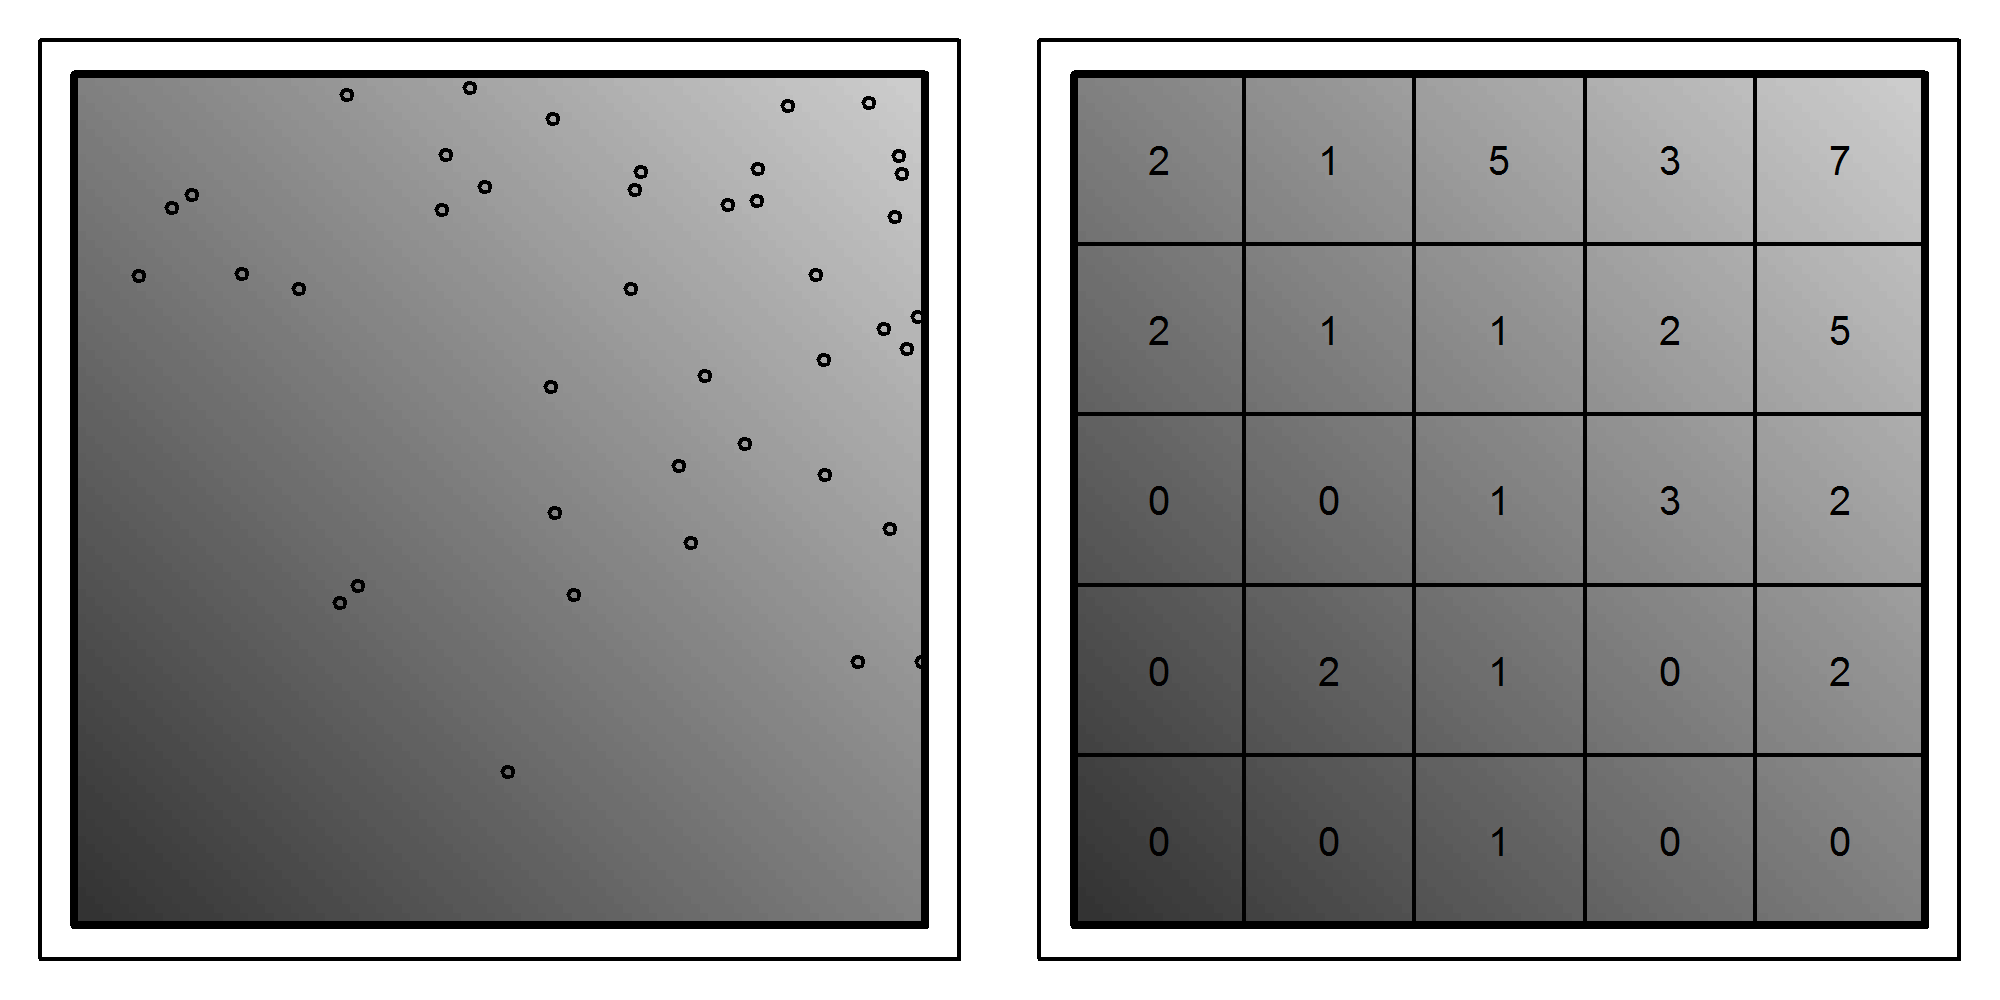
\includegraphics[width=\textwidth]{Ch13-Statespace/figs/heteroPlots}
\label{state-space.fig.hetero}
\caption{An example of a spatial covariate, say elevation, and a
  realization from an inhomogeneous Poisson point process with
  $\mu(\mathbf{s}, \bm{\beta}) = \exp(\beta_0 + \beta_1
  \mbox{ELEV}(\mathbf{s}))$ where $\beta_0=-6$ and $\beta_1=1$.}
\end{figure}

The 41 simulated points are shown in
Fig~\ref{state-space.fig.hetero}. High elevations
are represented by light gray and low elevations are darker. The
density of points in apparently higher in lighter regions
suggesting that these simulated animals prefer high
elevations.  %Perhaps they are mountain goats.
%The underlying model describing this preference is
%$\log(\mu(s)) = \exp(\beta \times elev(s))$
%where $\beta=2$ is the parameter to be estimated.
Given these points, we will now estimate $\beta_0$ and $\beta_1$ by
minimizing the negative-log-likelihood using \R's \verb+optim+
function.

\begin{samepage}
\begin{small}
\begin{verbatim}
nll <- function(beta) { # negative log-likelihood
    beta0 <- beta[1]
    beta1 <- beta[2]
    EN <- cuhre(2, 1, mu, beta0=beta0, beta1=beta1)$value
    -(sum(beta0 + beta1*elev.fn(s)) - EN)
}
starting.values <- c(0, 0)
fm <- optim(starting.values, nll, hessian=TRUE)
cbind(Est=fm$par, SE=sqrt(diag(solve(fm$hessian)))) # estimates and SEs
\end{verbatim}
\end{small}
\end{samepage}
Maximizing the likelihood took a fraction of a second, and we
obtained estimates of $\hat{\beta}_0=-5.93$ and $\hat{\beta}_1=0.95$,
which are very close to the data generating values. The 95\% confidence
interval for $\hat{\beta}_1$ is [0.61, 1.3] and since it does not
include zero, the null hypothesis that $\beta_1=0$, i.e. that there is
no effect of elevation on density, can be rejected. In addition to testing
hypotheses, these results can be used to predict population size in
new regions or create predicted density surface maps by plugging the
parameter estimates into Eqs.~\ref{state-space.eq.loglin} and~\ref{state-space.eq.EN}.

This example demonstrates
that if we had the data we wish we had, i.e. if we knew the
coordinates of the activity centers, we could easily estimate the
parameters governing the underlying point process and make inferences
about spatial variation in density and abundance. Unfortunately, in
virtually all animal ecology studies, including
SCR, the locations of the $N$ animals, or the $N$ activity centers,
cannot be directly observed. Thus we need
extra information to estimate the locations of these unobserved
points. In SCR, this information comes from the locations where each
animal is captured.

\section{Fitting inhomogeneous point process SCR models}

\subsection{Continuous space}

% One of the nice things about hierarchical models is that they
% %allow us to
% break a complex problem up into a series of simpler conditional
% sub-models. The problem faced in the analysis of SCR data is that the
% underlying point process is not observed, and so an
% observation model is needed to describe how the observed data result from
% the latent activity centers. Thus, in SCR, we can simply add the methods described above into a likelihood
% function or an MCMC algorithm to simulate the posterior distributions of $\beta$ conditional on the
% simulated values of $\mathbf{s}$.

In this example, we will use the same set of points simulated in the
previous section to generate spatial capture-recapture
data. Specifically, we overlay a grid of 49
traps on the map shown in Fig.~\ref{state-space.fig.hetero} and
simulate capture histories conditional upon the activity
centers. Then, we will attempt to estimate the activity center
locations as though we did not know where they were, as is the case in
real applications. We will also estimate $\beta_0$ and $\beta_1$ as
before and see how the estimates compare when the points are not
actually observed. The following \R~code simulates encounter histories under a
Poisson observation model (see Chapt. \ref{chapt.poisson-mn}), which could be appropriate in camera
trapping studies or when using other methods in which animals could
be detected multiple times at a trap during a single occasion.

\begin{samepage}
\begin{small}
\begin{verbatim}
xsp <- seq(20, 80, by=10); len <- length(xsp)
X <- cbind(rep(xsp, each=len), rep(xsp, times=len)) # traps
ntraps <- nrow(X); noccasions <- 5
y <- array(NA, c(N, ntraps, noccasions)) # capture data
sigma <- 5  # scale parameter
lam0 <- 1   # basal encounter rate
lam <- matrix(NA, N, ntraps)
set.seed(5588)
for(i in 1:N) {
    for(j in 1:ntraps) {
        # The object "s" was simulated in previous section
        distSq <- (s[i,1]-X[j,1])^2 + (s[i,2] - X[j,2])^2
        lam[i,j] <- exp(-distSq/(2*sigma^2)) * lam0
        y[i,j,] <- rpois(noccasions, lam[i,j])
    }
}
# data augmentation
nz <- 80; M <- nz+nrow(y)
yz <- array(0, c(M, ntraps, K))
yz[1:nrow(y),,] <- y # Fill data augmentation array
\end{verbatim}
\end{small}
\end{samepage}

Now that we have a simulated capture-recapture dataset \texttt{y} and we have
augmented it to create the new data object \texttt{yz}, we can
estimate the parameters using MCMC.  A commented Gibbs sampler written
in \R~is available in the accompanying \R~package \scrbook~(see
\texttt{?scrIPP}). This function is not meant to be an all purpose
tool for fitting SCR models using MCMC---instead, it is presented so
that interested readers can better understand the computational
aspects of the problem and can modify it for their purposes.
The function can be used as so:
%\begin{samepage}
\begin{small}
\begin{verbatim}
set.seed(3434)
fm1 <- scrIPP(yz, X, M, 10000, xlims=c(0,100), ylims=c(0,100),
              space.cov=elev.fn,
              tune=c(0.4, 0.2, 0.3, 0.3, 7))
plot(mcmc(fm1$out))
\end{verbatim}
\end{small}
%\end{samepage}
which requests 10000 posterior samples and estimates the effect of the
spatial covariate, elevation, on density. Currently, the function
places uniform priors on the parameters $\sigma$, $\lambda_0$,
$\beta_0$ and $\beta_1$, although this could easily be modified. Note that any spatial
covariate that returns a real value for any location in the
state-space can be supplied using the \texttt{space.cov} argument. The resulting
trace plots of the Markov chains and the posterior distributions for
three parameters are
shown in Fig.~\ref{state-space.fig.fm1post}. The chains appear to
converge rapidly but may need to be run longer to reduce Monte Carlo
error.

\begin{figure}
  \centering
  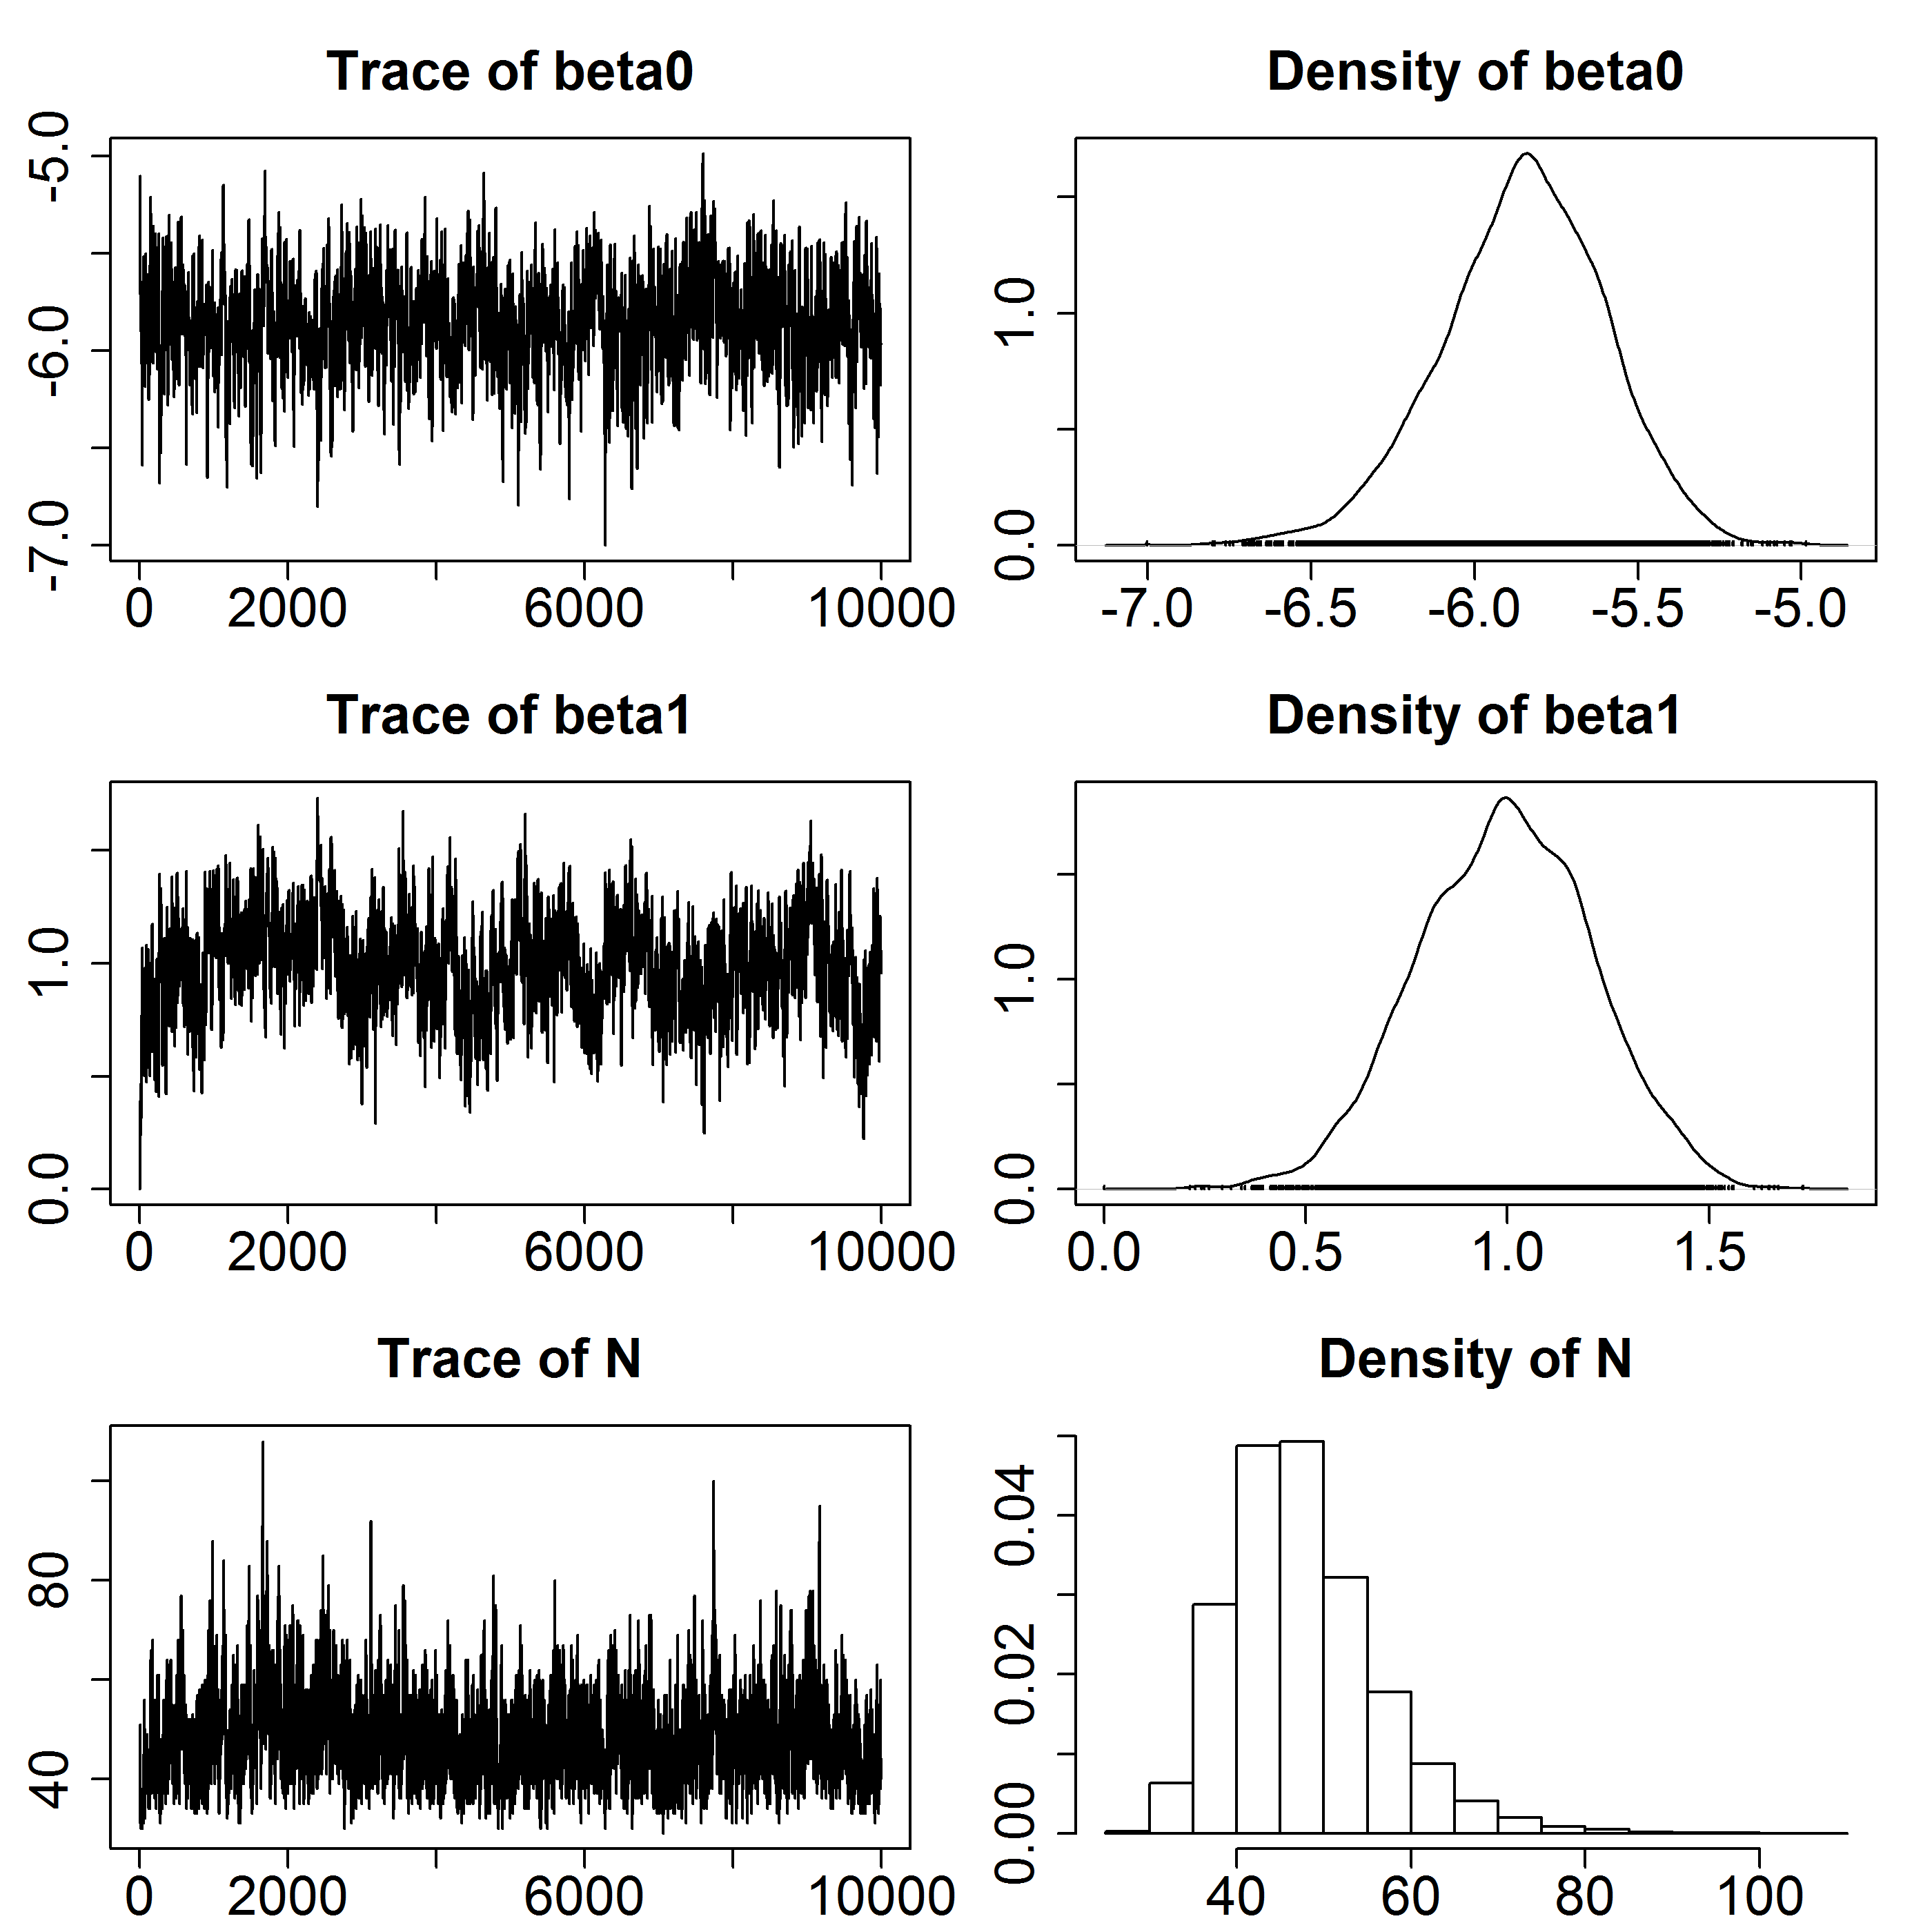
\includegraphics[width=0.8\textwidth]{Ch13-Statespace/figs/fm1p}
  \caption{Trace plots and posterior distributions from MCMC analysis
    of SCR model with inhomogeneous point process. Analysis was
    conducted using the \texttt{scrIPP} function in the accompanying
    \R~package \scrbook.}
  \label{state-space.fig.fm1post}
\end{figure}
%For comparison, we also fit this model using $\texttt{secr}$. See the
%help file \texttt{Ch-IPP} in \scrbook~ for \R~commands necessary to
%prepare the data for \secr.

\begin{table}%[b]
\centering
\caption{Summary of posterior distributions from SCR model with
  inhomogeneous point process. }
\begin{tabular}{lrrrr}
\hline
Parameter 	 	& Mean  	& SD    	& 2.5\% 	& 97.5\% \\
\hline
 $\sigma=5$ 	 	&  5.232 	&  0.310 	&  4.681 	&  5.858 \\
 $\lambda_0=1$ 	 	&  0.802 	&  0.119 	&  0.595 	&  1.049 \\
 $\beta_0=-6$ 	 	& -5.856        & 0.2542        & -6.376        & -5.393 \\
 $\beta_1=1$ 	 	&  0.985 	&  0.209 	&  0.575 	&  1.378 \\
 $N=41$ 	 	& 47.615 	&  8.041 	& 35.000 	& 66.000 \\
 $\mathbb{E}[N]=39.9$ 	& 47.551 	& 10.992 	& 29.837 	& 71.332 \\
\hline
\end{tabular}
\label{state-space.tab.simIPP}
\end{table}

Summaries of the posterior distributions are presented in
Table~\ref{state-space.tab.simIPP}. The posterior means for $\beta_0$
and $\beta_1$ are quite similar to MLEs from the analysis in the
previous section in which we assumed no observation error. However, we
see that the confidence intervals are wider. With respect to the other
parameters in the model, we see that all of the data
generating parameter fall within the 95\% credible intervals. One
interesting thing to note is that, although the point estimates for
the expected and realized values of $N$ are quite similar, the
estimate is more precise for the realized value. This is to be
expected because the uncertainty associated with the realized value of
$N$ is entirely determined by the encounter rate parameters. That is,
if we could perfectly detect all of the individuals in $\cal S$, there
would be no uncertainty about $N$. In contrast, the variance for
expected value of $N$ is affected by the variance of all the parameters
in the model, not just the encounter rate parameters. See
\citet{efford_fewster:2012} for additional discussion on the
difference between realized and expected values of abundance.
%, and we see that the point
%estimates and confidence/credible intervals are quite similar from the
%MCMC and maximum likelihood (ML) analyses. One exception is that the
%confidence intervals for $N$ and the expected value of $N$ are
%somewhat different. This may result from the fact that the MCMC
%analysis assumed a binomial prior for $N$, whereas the ML analysis
%assumed a Poisson prior.


Fitting continuous space inhomogenous point process models is somewhat
difficult in \bugs~because the ``IPP'' prior $[\mathbf{s}_i | \bm
\beta]$---unlike the uniform prior---is not one of the
available distributions that comes with the software. It is
possible to add new distributions in \bugs, but it is somewhat
cumbersome.  \secr~allows
users to fit continuous space models using linear or polynomial functions of the x- and y-
coordinates, but it does not accept truly continuous covariates that
are functions of space. However, these
are not really important limitations because discrete
space versions of the model are straight-forward, and virtually all spatial
covariates are, or can be, defined as such.

\subsection{Discrete space}
\label{modeling.sec.discrete}

To fit inhomogeneous point process models using covariates in discrete
space, i.e. in raster format, we follow the same steps
as outlined in Chapter~\ref{chapt.poisson-mn}---we define ${\bf s}_i$ as
pixel ID, and we use the categorical distribution as a prior. This
effectively changes the problem from estimating the coordinates of an
activity center, to estimating the pixel in which an activity center is
located. As pixel size approaches zero, these two become equivalent. A good
example is found in \citep{mollet_etal:2012}. Here we present
an analysis of the simulated data shown in the %right panel of
Fig.~\ref{state-space.fig.hetero}. The spatial covariate, let's call it
forest canopy height (CANHT), was simulated
using using the code shown on the help page
\verb+ch11+ in \scrbook. The points are the number of
activity centers in each pixel, generated from a single realization of
the inhomogeneous point process model with intensity
$\mu(\mathbf{s}, \bm{\beta}) = \exp(\beta_0 + \beta_1
\text{CANHT}({\bf s}))\times\text{pixelArea}$,
where $\beta_0 = -6$ and $\beta_1 = 1$.
\begin{figure}[ht]
\centering
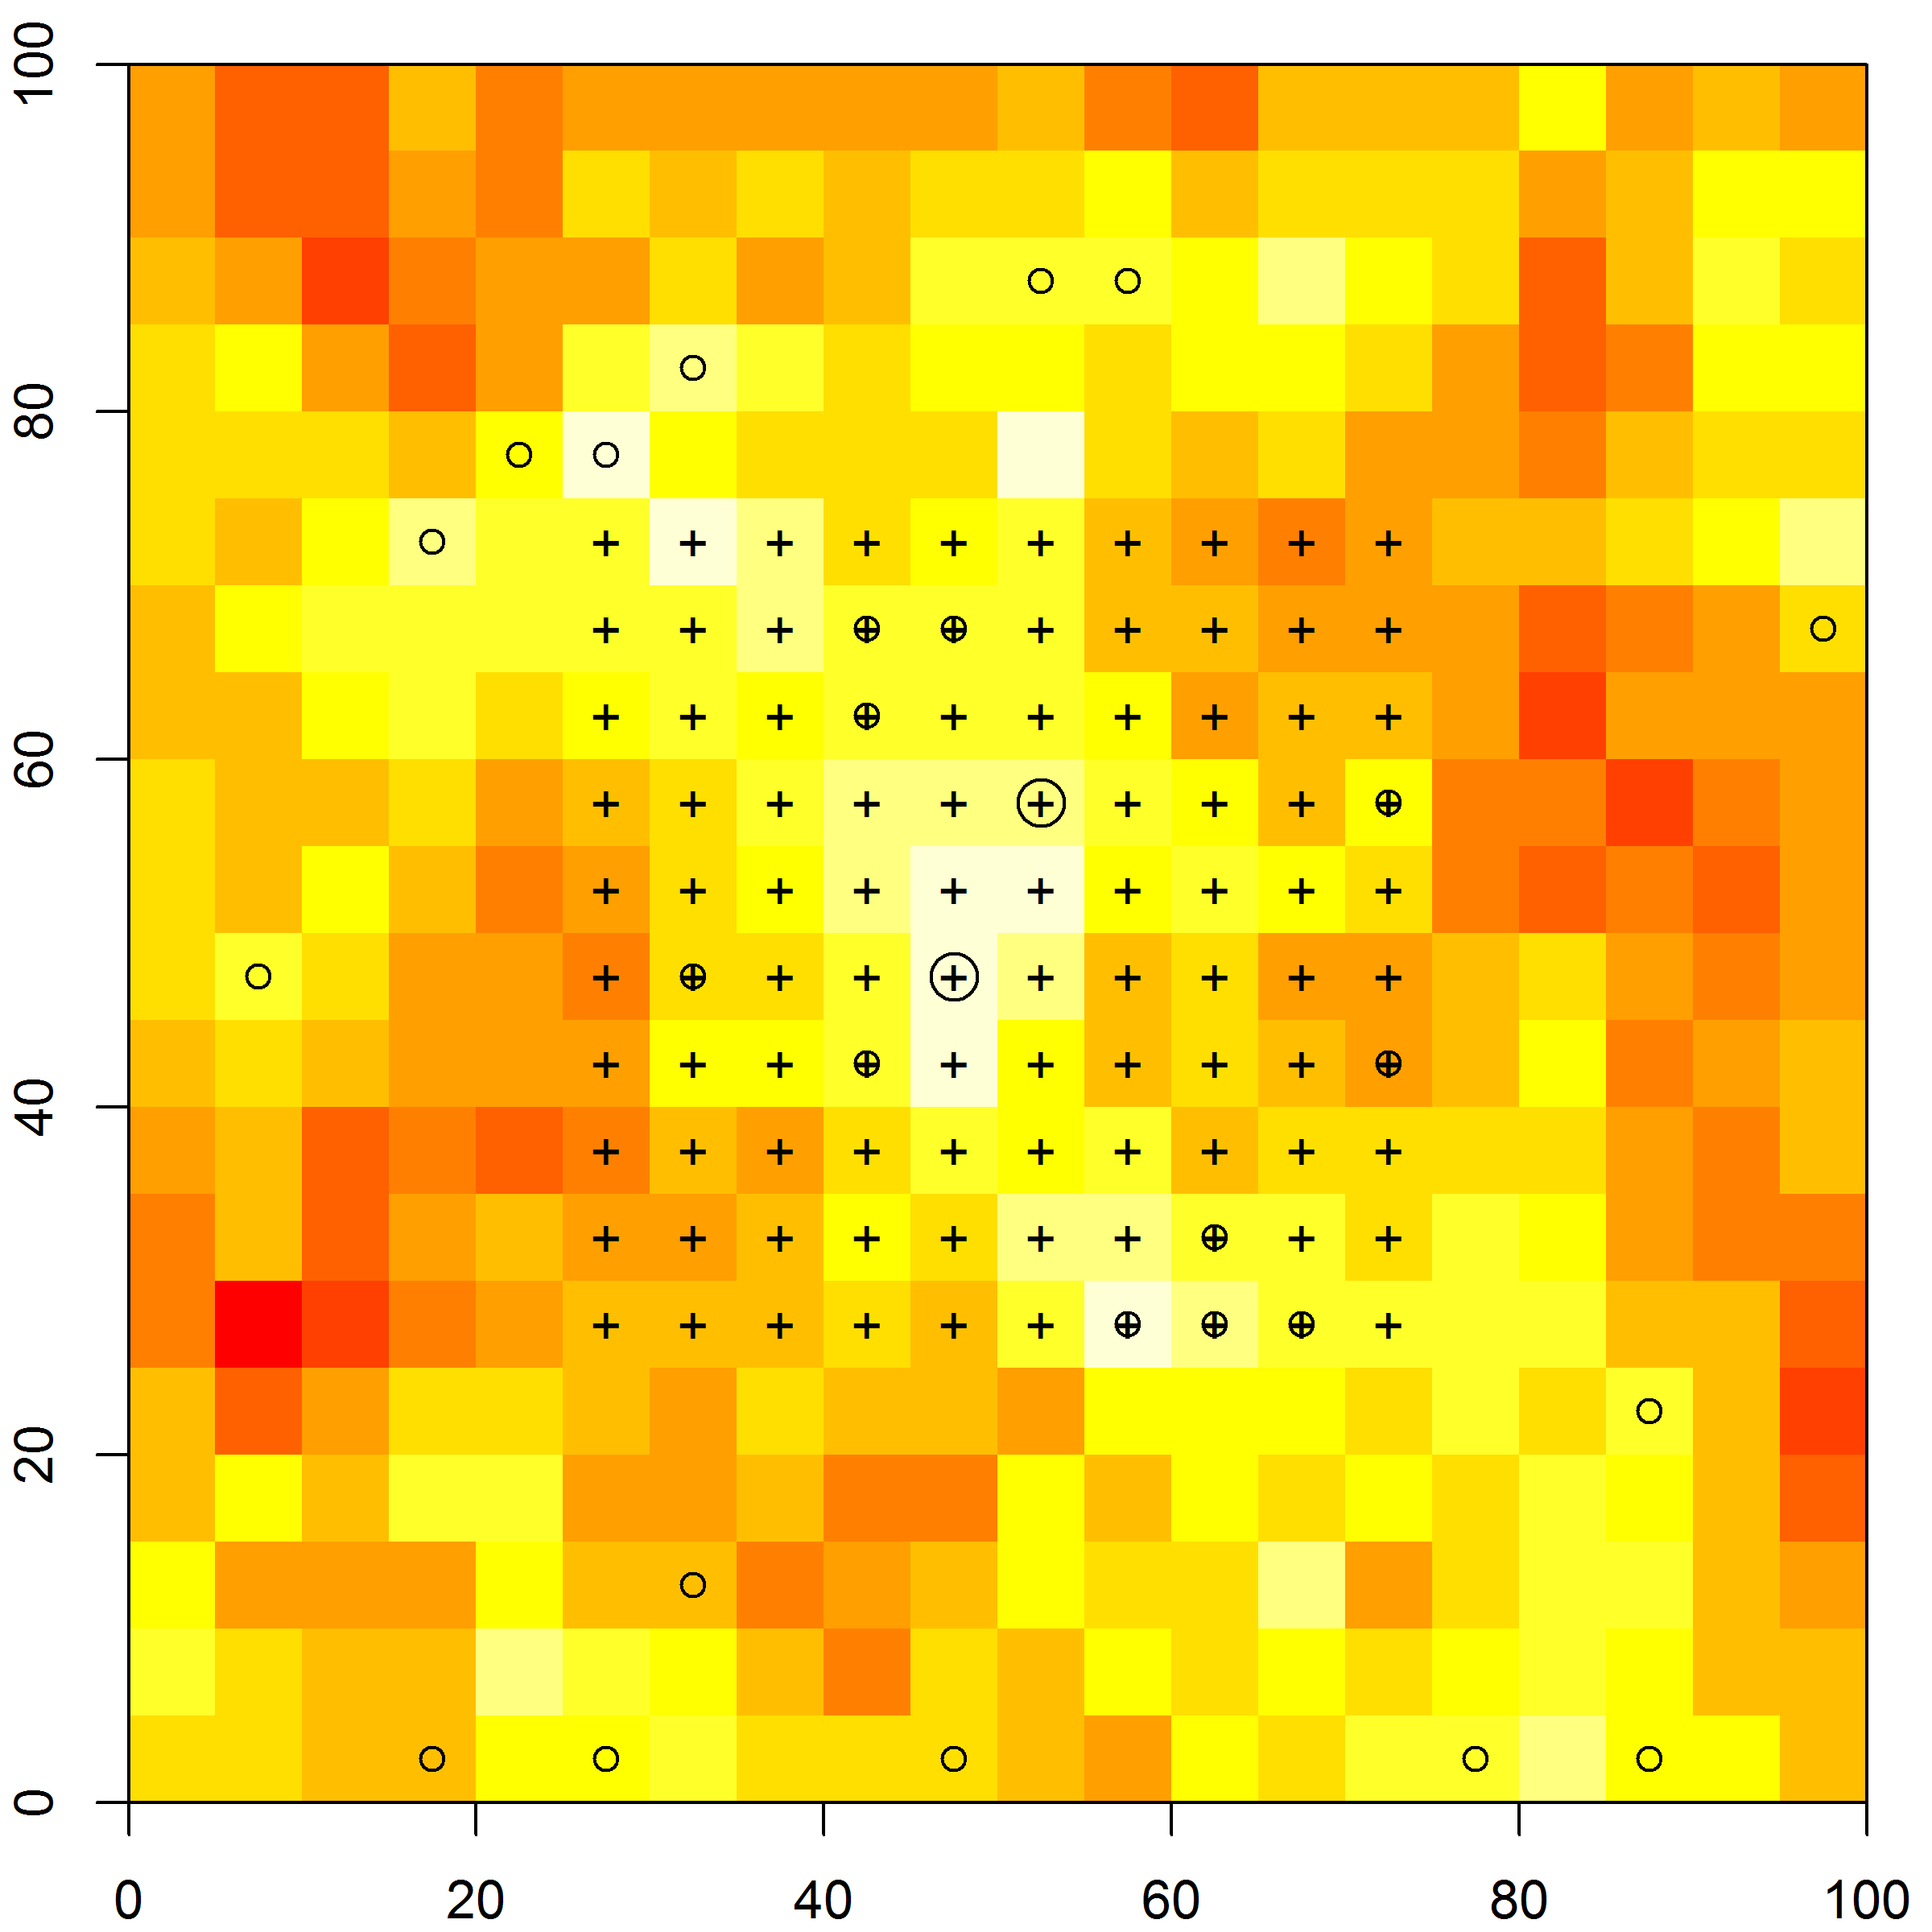
\includegraphics[width=0.6\textwidth]{Ch13-Statespace/figs/discrete}
\label{state-space.fig.discrete}
\caption{Simulated activity centers in discrete space. The spatial
  covariate, canopy height, is highest in the lighter areas and
  density increases with canopy height. A single
  activity center is shown as a small circle, and larger circles
  represent two activity centers in a pixel. Trap locations
  are shown as crosses.}
\end{figure}

The \bugs~description of the model is shown in
panel~\ref{state-space.panel1}. The vector \verb+probs[]+ is the prior
probability defined by Eq.~\ref{state-space.eq.pdf.hetero.d}, which is
the probability that an individual's activity center is located at
pixel $\bf s$. \verb+Sgrid+ is the matrix of coordinates for each pixel.

\begin{panel}%[h!]
\centering
\rule[0.15in]{\textwidth}{.03in}
\begin{small}
\begin{verbatim}
model{
sigma ~ dunif(0, 20)
lam0 ~ dunif(0, 5)
beta0 ~ dunif(-10, 10)
beta1 ~ dunif(-10, 10)
for(j in 1:nPix) {
  mu[j] <- exp(beta0 + beta1*CANHT[j])*pixArea
  probs[j] <- mu[j]/EN
}
EN <- sum(mu[]) # Expected value of N, E[N]
psi <- EN/M
for(i in 1:M) {
  w[i] ~ dbern(psi)
  s[i] ~ dcat(probs[])
  x0g[i] <- Sgrid[s[i],1]
  y0g[i] <- Sgrid[s[i],2]
  for(j in 1:ntraps) {
    dist[i,j] <- sqrt(pow(x0g[i]-traps[j,1],2) + pow(y0g[i]-traps[j,2],2))
    lambda[i,j] <- lam0*exp(-dist[i,j]*dist[i,j]/(2*sigma*sigma)) * w[i]
    y[i,j] ~ dpois(lambda[i,j])
    }
  }
N <- sum(w[]) # Realized value of N
}
\end{verbatim}
\end{small}
\rule[0.15in]{\textwidth}{.03in}
\caption{\bugs~code for fitting inhomogeneous point process model in
  discrete space.}
\label{state-space.panel1}
\end{panel}

This model can also be fit in \secr, which refers
to the raster data as a ``habitat mask''. \R~code to format the data
and fit the models using \secr~and \jags~is available in \scrbook---see
\verb#help(ch9secrYjags)#. Results of the
comparison are shown in Table \ref{state-space.tab.jagsVsecr} and are
similar as expected. The differences that do exist can be
explained by a variety of reasons. For one, there exists some Monte
Carlo error in the Bayesian posterior summaries. There is also the
fact that posterior summaries can be computed in numerous ways---for
example, we could have presented posterior modes or medians instead of
means---or, we could have shown highest posterior density credible
intervals instead of simple percentiles. The posteriors would also
differ if we chose more informative priors than the uniform
distributions used here. We see no reason why these
issues should be seen as limitations of the Bayesian analysis, rather
we would argue that the posterior distribution, which describes the
probability that the parameter equals any particular value, is a
better descriptor uncertainty than any particular point estimator or
confidence interval. %Futhermore, most of these differences are minor,
%and hardly worth mention.
% The only exception is that the estimates of
% the expected and realized values of $N$ are closer to the data
% generating values in the Bayesian analysis, and the Bayesian credible
% intervals are narrower than the frequentist confidence intervals. This
% is likely a result of the fact that the Bayesian analysis assumed
% that $N$ was binomial whereas the frequentist analysis
% assumed a Poisson prior for $N$, and the variance of the binomial will
% always be less than or equal to the variance of Poisson distribution
% for a shared expectation.

\begin{table}%[h!]
\centering
\caption{Comparison of \secr~and \jags~results. Point estimates from
  the Bayesian analysis are posterior means. Intervals are lower and
  upper 95\% CIs.}
\begin{tabular}{lrlrrrr}
\hline
Parameter 	& Truth 	& Software 	& Mean 	& SD 	& 2.5\% & 97.5\% \\
\hline
 $\lambda_0$ 	&  1.00 	& \textbf{JAGS} 	&  1.04 	& 0.087 	&  0.88 	&  1.22 \\
  	&  1.00 	& \texttt{secr} 	&  1.08 	& 0.089 	&  0.92 	&  1.27 \\
 $\sigma$ 	& 10.00 	& \textbf{JAGS} 	& 10.16 	& 0.373 	&  9.46 	& 10.94 \\
  	& 10.00 	& \texttt{secr} 	&  9.84 	& 0.350 	&  9.18 	& 10.55 \\
 $\beta_1$ 	&  1.00 	& \textbf{JAGS} 	&  1.20 	& 0.350 	&  0.50 	&  1.88 \\
  	&  1.00 	& \texttt{secr} 	&  1.09 	& 0.316 	&  0.47 	&  1.71 \\
 $N$ 	& 30.00 	& \textbf{JAGS} 	& 26.63 	& 2.585 	& 23.00 	& 33.00 \\
  	& 30.00 	& \texttt{secr} 	& 28.19 	& 3.037 	& 24.49 	& 37.39 \\
 $\mathbb{E}[N]$ 	& 32.30 	& \textbf{JAGS} 	& 26.39 	& 5.048 	& 17.25 	& 36.96 \\
  	& 32.30 	& \texttt{secr} 	& 28.19 	& 6.117 	& 18.52 	& 42.93 \\
\hline
\end{tabular}
\label{state-space.tab.jagsVsecr}
\end{table}


\section{Ecological Distance and Density Covariates}

Habitat characteristics that affect spatial variation in density can
also affect home range size and movement behavior. For example, a
species that occurs at high density in a forest may be reluctant to
venture from a forest patch into an adjacent field. Thus, even if a
trap placed in a field is located very close to an animal's activity
center, the probability of capture may be very
low. In this case, forest cover is a covariate of
both density and encounter probability,
and we could model it as such by combining the methods described in
this chapter with those described in Chapter~\ref{chapt.ecoldist}.

To demonstrate, we continue with our analysis of the data shown in
Fig~\ref{state-space.fig.discrete}. Once again, we suppose that density
increases with canopy height, but this time, we also make the
assumption that home range size decreases as density increases. This
commonly-observed phenomenon can be explained by numerous factors such
as intra-specific competition \citep{sillett_etal:2004} or optimal
foraging behavior \citep{tufto_etal:1996,said_servanty:2005}. To model
this effect, we
introduce the parameter $\theta$, which determines the ``cost'' of
moving between pixels. If $\theta=0$, then the animal perceives
distance as Euclidean. If $\theta>0$, then least-cost distance (LCD)
is greater than than Euclidean distance (ED). In most cases, we would
not expect,
or should not even consider the possibility of $\theta<0$ because this
implies that LCD$<$ED, which would mean that an animal could view
1000km as 1m. In addition to the fact that this is not biologically
justifiable, it also suggests that the area of the state-space could
be infinitely large. Thus, one may want to enforce the constraint that
$\theta$ is $\geq 0$. See Chapter~\ref{chapt.ecoldist} for
more details.

A question that arises is: Is possible to estimate $\bm \beta$
and $\theta$ using standard SCR data? In other words, can we model
spatial variation in density and connectivity at the same time,
using standard SCR data? Currently, it is not possible to
model least-cost distance using \jags~or \secr, so we wrote our own
function, \verb+scrDED+, to fit the model using maximum likelihood. An
example analysis is provided on the help page for the function in our
\R~package \scrbook. We briefly note here that the function requires
the capture history data, the trap locations, and the raster data
formatted using the {\tt raster} package
\citep{hijmans_vanetten:2012}. The linear model for the
intensity parameter $\mu(\mathbf{s}, \beta)$ and the least-cost distance
function $\text{lcd}(\theta)$ are specified using \R's formula interface. A
simple function call is
\begin{verbatim}
fm <- scrDED(y, traplocs=X, den.formula=~elev, dist.formula=~elev,
             rasters=elev.raster)
\end{verbatim}
To assess the possibility of estimating both $\bm \beta$ and $\theta$, we
conducted a small simulation study, generating 500 datasets from the
model with both parameters set to 1, which corresponds to the
conditions described above. The results indicate that it is
possible to estimate both parameters
(Fig~\ref{ch9.fig.sim}).

\begin{figure}[ht]
\centering
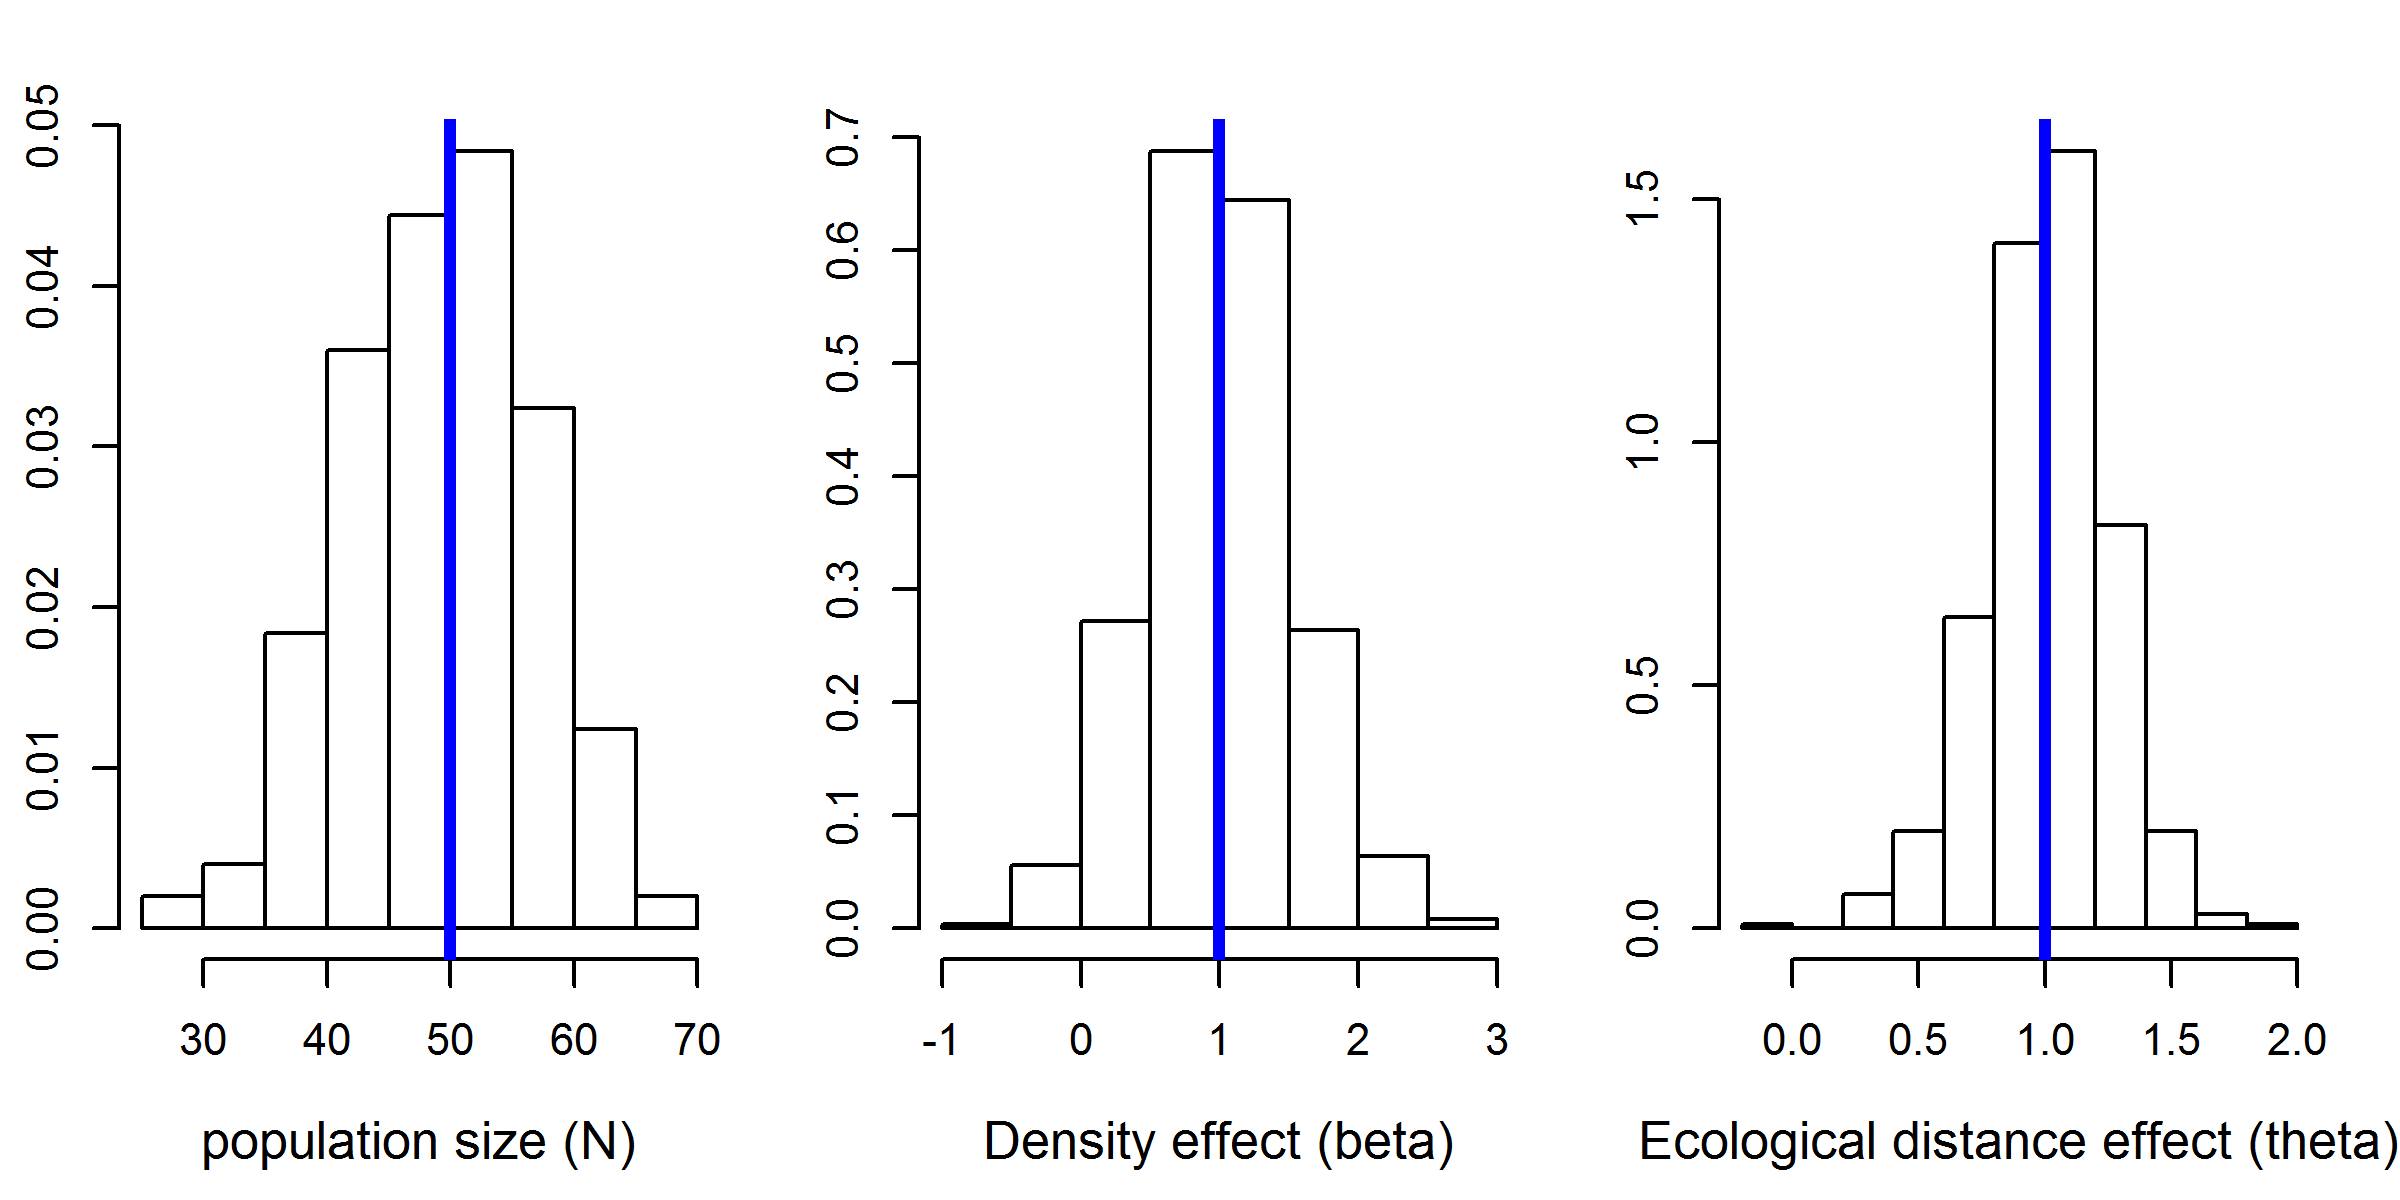
\includegraphics[width=4in,height=2in]{Ch13-Statespace/figs/scrDEDsim}
\caption{Histograms of parameter estimates from 500 simulations under
  the model in which both density and ecological distance are affected
by the same covariate, canopy height. The vertical lines indicate the
data-generating value.}
\label{ch9.fig.sim}
\end{figure}


\section{The Jaguar Data}

Estimating density of large felines has been a priority for many
conservation organizations, but few robust methodologies existed before
the advent of SCR. Distance sampling is not feasible for such rare and
cryptic species, and traditional capture-recapture methods yield
estimates that are highly sensitive to the subjective choice of the
effective survey area. SCR models provide a powerful alternative
because density can be estimated directly and data can be collected
using non-invasive methods such as camera traps or hair snares.

In this example, we demonstrate how readily density can be estimated
for a globally imperiled species using SCR. Furthermore, we show how
inhomogeneous point process models can be used to test important
hypotheses regarding the factors affecting density.
The data come from an 8-year camera-trapping study designed to assess the impacts of poaching
on jaguar density in Argentina, near the borders of Brazil and
Paraguay. Additional information about the study is presented in
\citet{paviolo_etal:2008} and \citet{paviolo_etal:2009}. Although
jaguars themselves are occasionally killed by
poachers, the larger concern is the influence of poaching on prey
species. To protect jaguars and related species, protected areas have
been established and three levels of protection are
recognized as depicted in Fig.~\ref{state-space.fig.jaguarCts}. The dark green
area is the Iguaz\'{u} National Park that is patrolled regularly by law enforcement
officials. The light green areas are officially protected, but due to
resource limitations, are not patrolled as often. The beige areas are
not protected at all, and the gray areas are large soybean
monocultures, which provide no habitat.

To test for differences in
density between the three regions, we modeled the point process intensity parameter
as a function of protection status (PROTECT), which we treated as an
ordinal variable: $\mu(\mathbf{s}, \bm{\beta}) = \exp(\beta_0 +
\beta_1\text{PROTECT}(\mathbf{s}))$. We hypothesized that $\beta_1 > 0$
indicating that jaguar density increases with protection status. In
addition to modeling spatial variation in density, we also modeled the
scale parameter of the half-normal or Gaussian encounter model as
sex-specific, since male cats typically have larger home ranges than
females \citep{sollmann_etal:2011}. Since sex is an
individual-specific covariate, and not observed for the individuals
that were not captured, a prior is required for the sex of uncaptured
individuals. We used an Bernoulli prior with probability 0.5 to
describe our uncertainty about sex ratio.

\begin{figure}%[ht]
\centering
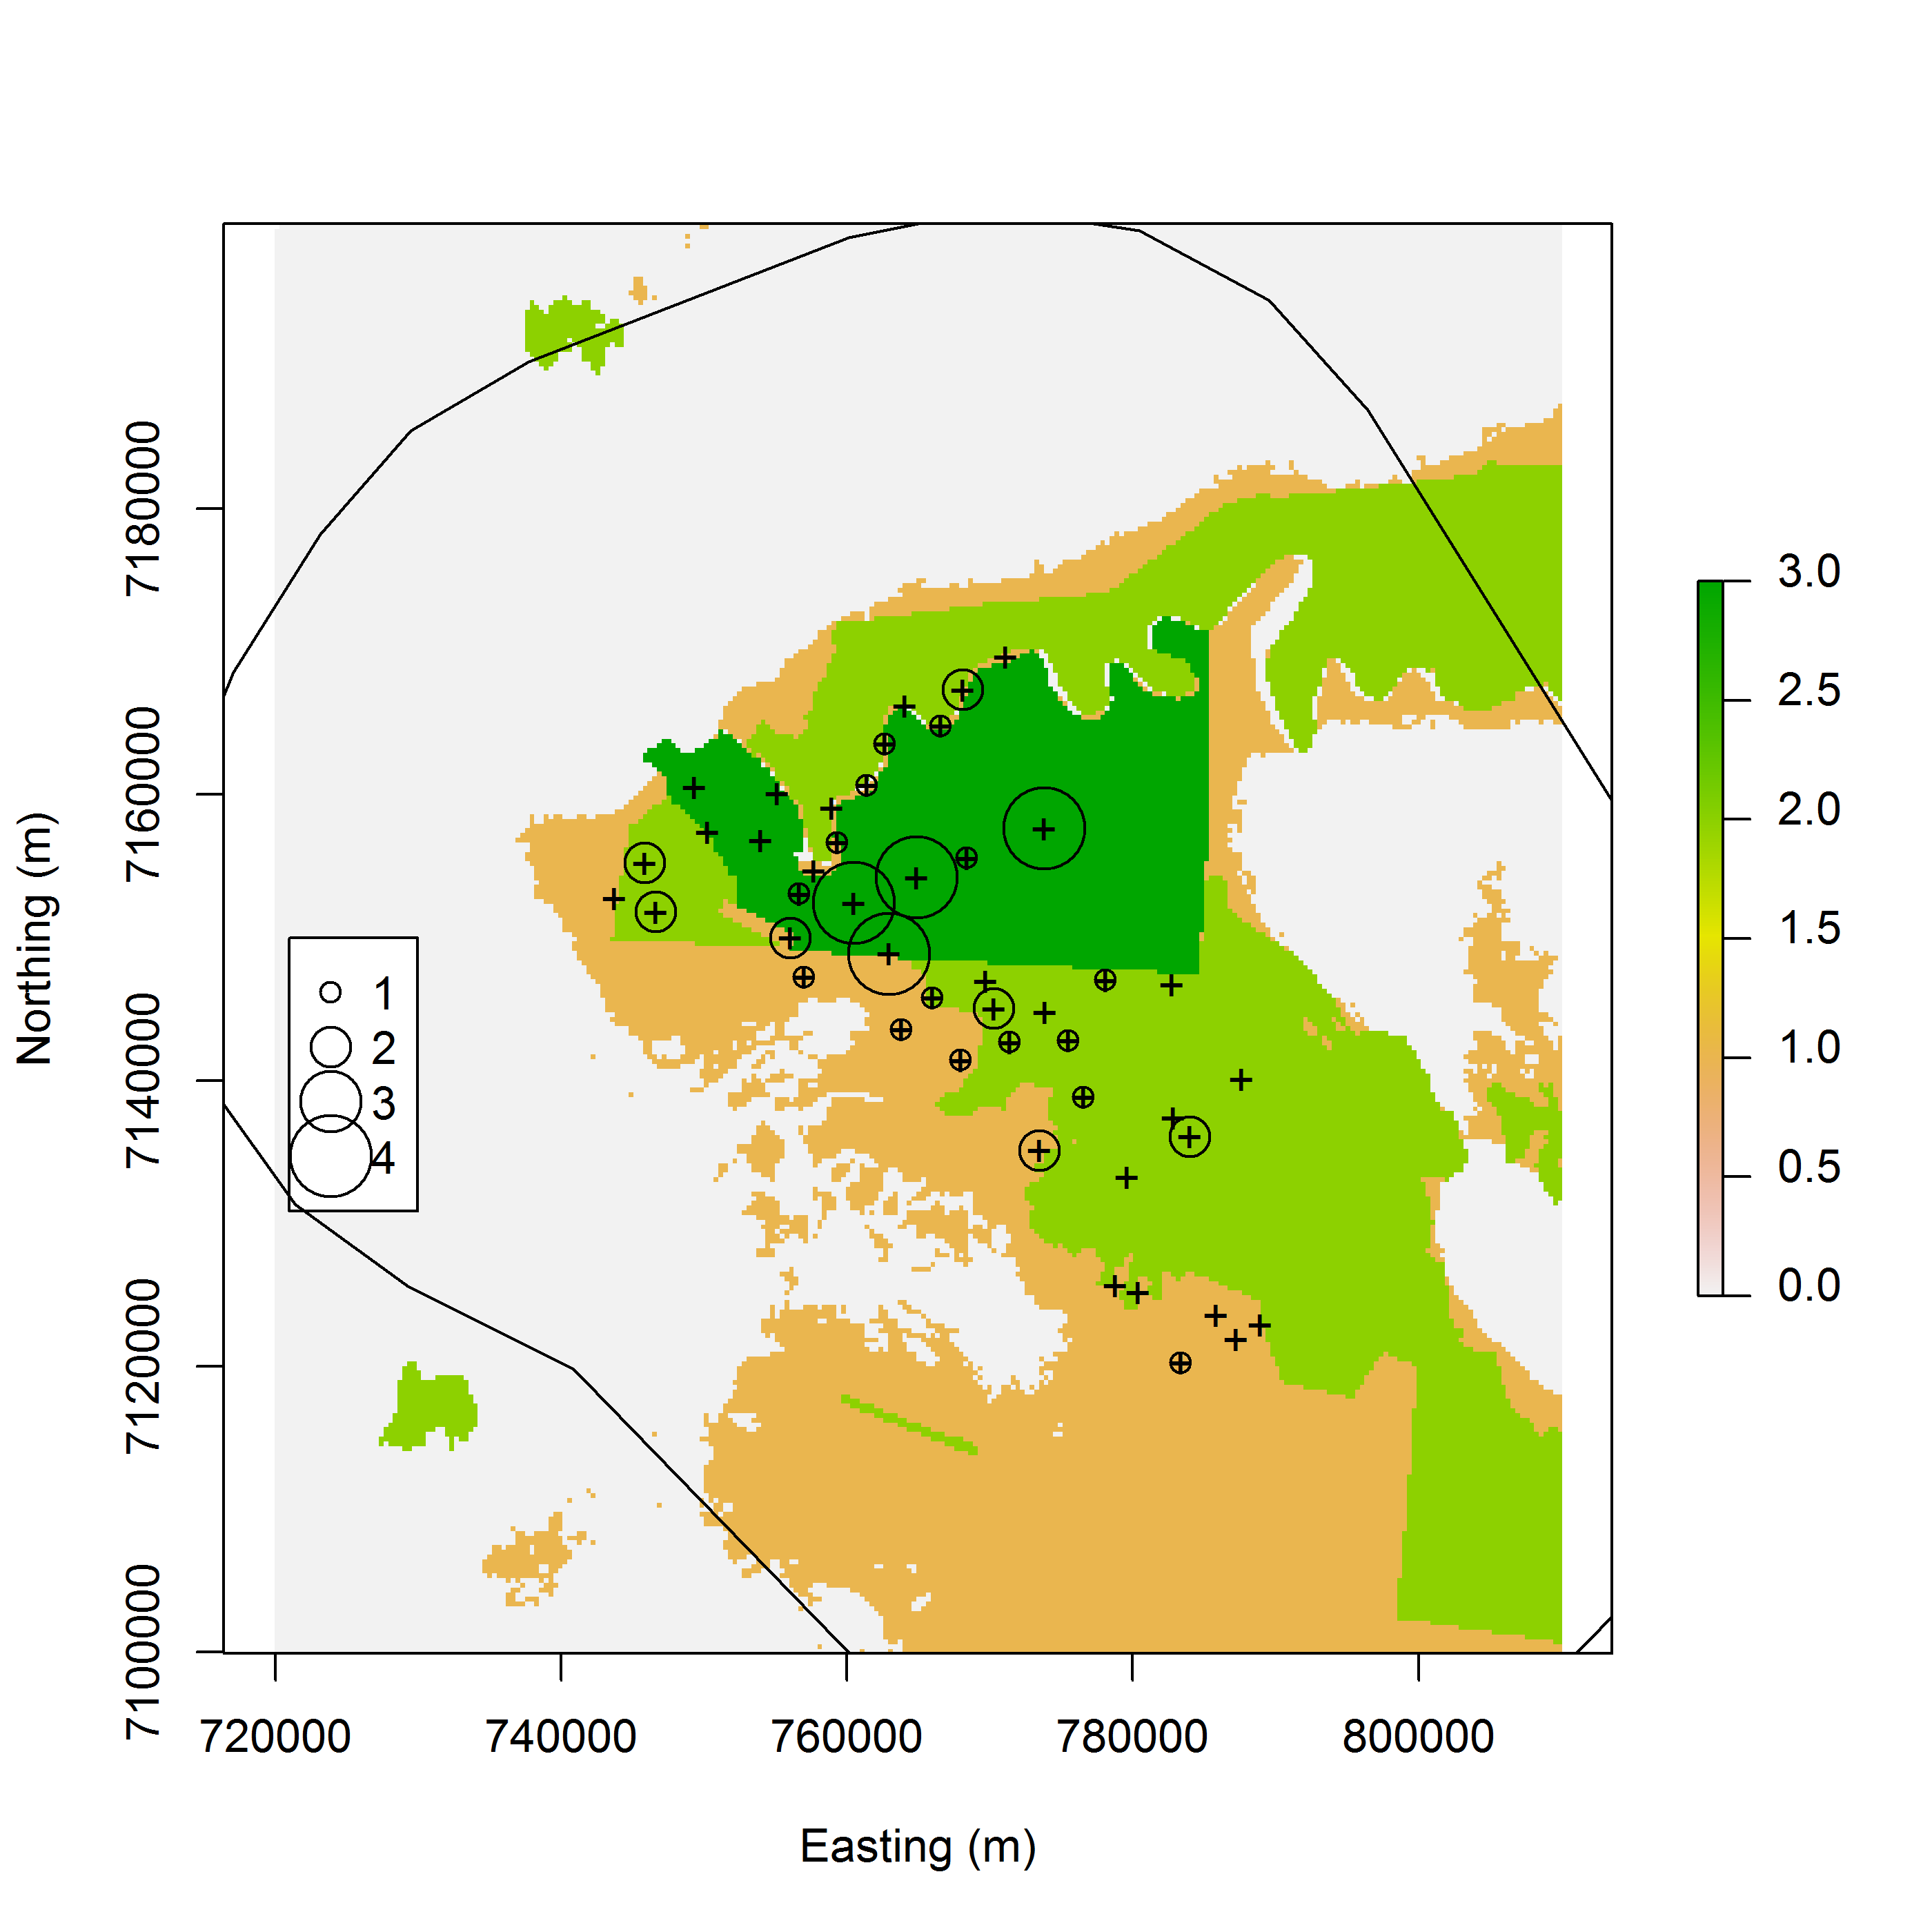
\includegraphics[width=0.6\textwidth]{Ch13-Statespace/figs/jaguarCountMap}
\label{state-space.fig.jaguarCts}
\caption{Jaguar detections at 46 camera trap stations. The three levels of
  protection status are no protection (beige), some protection (light
  green), and Iguaz\'{u} National Park (dark green). Non-habitat
  (soybean monocultures) is shown in gray. }
\end{figure}

The geometry of the state-space differs greatly from the simple square
regions that we have considered throughout this chapter, which raises
a few questions. First, how would one integrate
Eq.~\ref{state-space.eq.pdf.hetero} over a
complex spatial region? Earlier we used the function \verb+cuhre+ in
\R~for the two-dimensional integration, but its \verb+lower+ and
\verb+upper+ arguments essentially assume that the state-space is
square. There are methods of transforming the state-space to make this
work, but once again we find that it is most convenient to work in
discrete space and sum over all the pixels defining
$\mathcal{S}$. In this example, we restricted the state-space to exclude the large
soybean monocultures surrounding the study area, and we only
considered area south of the Iguaz\'{u} River, which runs along the northern border
of the park shown in dark green in
Fig.~\ref{state-space.fig.jaguarCts}. Rather than restricting the
state-space, we could have modeled the permeability of the river using
the methods described in the previous section and in
Chapter~\ref{chapt.ecoldist}; however, no sampling was conducted on
the northern side of the river, and ancillary data indicates that
jaguars rarely forge the waterway.

We fit the model to data from a single year of data from 46
camera stations, each consisting of a pair of cameras placed along
roads or small trails. Forty-five detections of 16 jaguars (8 males and 8
females) were made over a 95-day sampling period. The mean number of
sampling days at each camera station was 48.2. The raw capture data
shown in Fig.~\ref{state-space.fig.jaguarCts} suggest that the highest
number of captures was in the national park, but there were also
several traps in the park with no captures. Furthermore, few cameras
were placed far from the protected areas, making it somewhat difficult
to detect differences in density. \R~code to fit the model is
available in \scrbook  on the help page \verb+jaguarDataCh9+.
Parameter estimates are shown in Table\ref{state-space.tab.jagposts}.


% To assess the influence of poaching on jaguar density, we treated
% protection status as an ordinal variable with 3 levels: no protection,
% some protection, and high protection (national parks). Clearly these
% are ordered, and our
% hypothesis is that poaching pressure should decrease and jaguar
% density should increase with the level of
% protection. Thus, $\beta$ in this example is a ``slope''
% parameter describing the degree to which protection status affects
% jaguar density. We also hypothesized that males would have larger home
% ranges than females  and that the sex ratio may not be
% 1:1.


\begin{table}
\centering
\caption{Summaries of posterior distributions from the model of jaguar
  density. $\sigma$ is the scale parameter of
  the half-normal detection function. $\lambda_0$ is base-line encounter rate. $\beta_1$ is the
  effect of protection status on jaguar density. $\rho$ is the
  sex-ratio.  $N$ is population size. The last three parameters are the density estimates
  (jaguars/100km$^2$) for the three levels of protection.}
\begin{tabular}{lrrrr}
\hline
& Mean & SD & 2.5\% & 97.5\% \\
\hline
 $\sigma_\text{female}$ 	& 5434.886 	& 883.7433 	& 4093.6069 	& 7549.062 \\
 $\sigma_\text{male}$ 	& 6208.341 	& 822.6217 	& 4881.4060 	& 8093.759 \\
 $\lambda_0$ 	&    0.013 	&   0.0036 	&    0.0068 	&    0.021 \\
 $\beta_0$ 	&   -4.667 	&   0.2866 	&   -5.2527 	&   -4.093 \\
 $\beta_1$ 	&    0.196 	&   0.3672 	&   -0.5179 	&    0.961 \\
 $\rho$ 	&    0.541 	&   0.0551 	&    0.4286 	&    0.644 \\
 $N$ 	        &   36.428 	&   9.6986 	&   23.0000 	&   61.000 \\
 $D_\text{low}$ 	&    0.921 	&   0.3851 	&    0.3789 	&    1.894 \\
 $D_\text{med}$ 	&    0.775 	&   0.3006 	&    0.2653 	&    1.503 \\
 $D_\text{high}$ &    1.444 	&   0.3325 	&    0.8791 	&    2.110 \\
 \hline
\end{tabular}
\label{state-space.tab.jagposts}
\end{table}

The results indicate that efforts to protect jaguars by reducing
poaching in protected areas are not working as well as hoped
for. The
posterior probability that $\beta_0 > 0$ was 0.705, and
the posterior mean of realized density was only 58\% higher in the national park than in the
unprotected area. Fig.~\ref{state-space.fig.Dsurface} shows the estimated
density surfaces. The first map is the expected density (posterior mean) in each of
the three values, which was computed by plugging in the posterior mean
values of $\beta_0$ and $\beta_1$ into the log-linear intensity
function. The second map is the realized density surface. Conditional
on the $N$, this is the probability distribution for the
number of activity centers in each pixel of the rasterized
state-space---here shown as the posterior mean. The expected values
would be used if we were interested in making inferences about other
areas or time periods, whereas the realized map is the best
description of the system during the study period.

\begin{figure}%[ht]
\centering
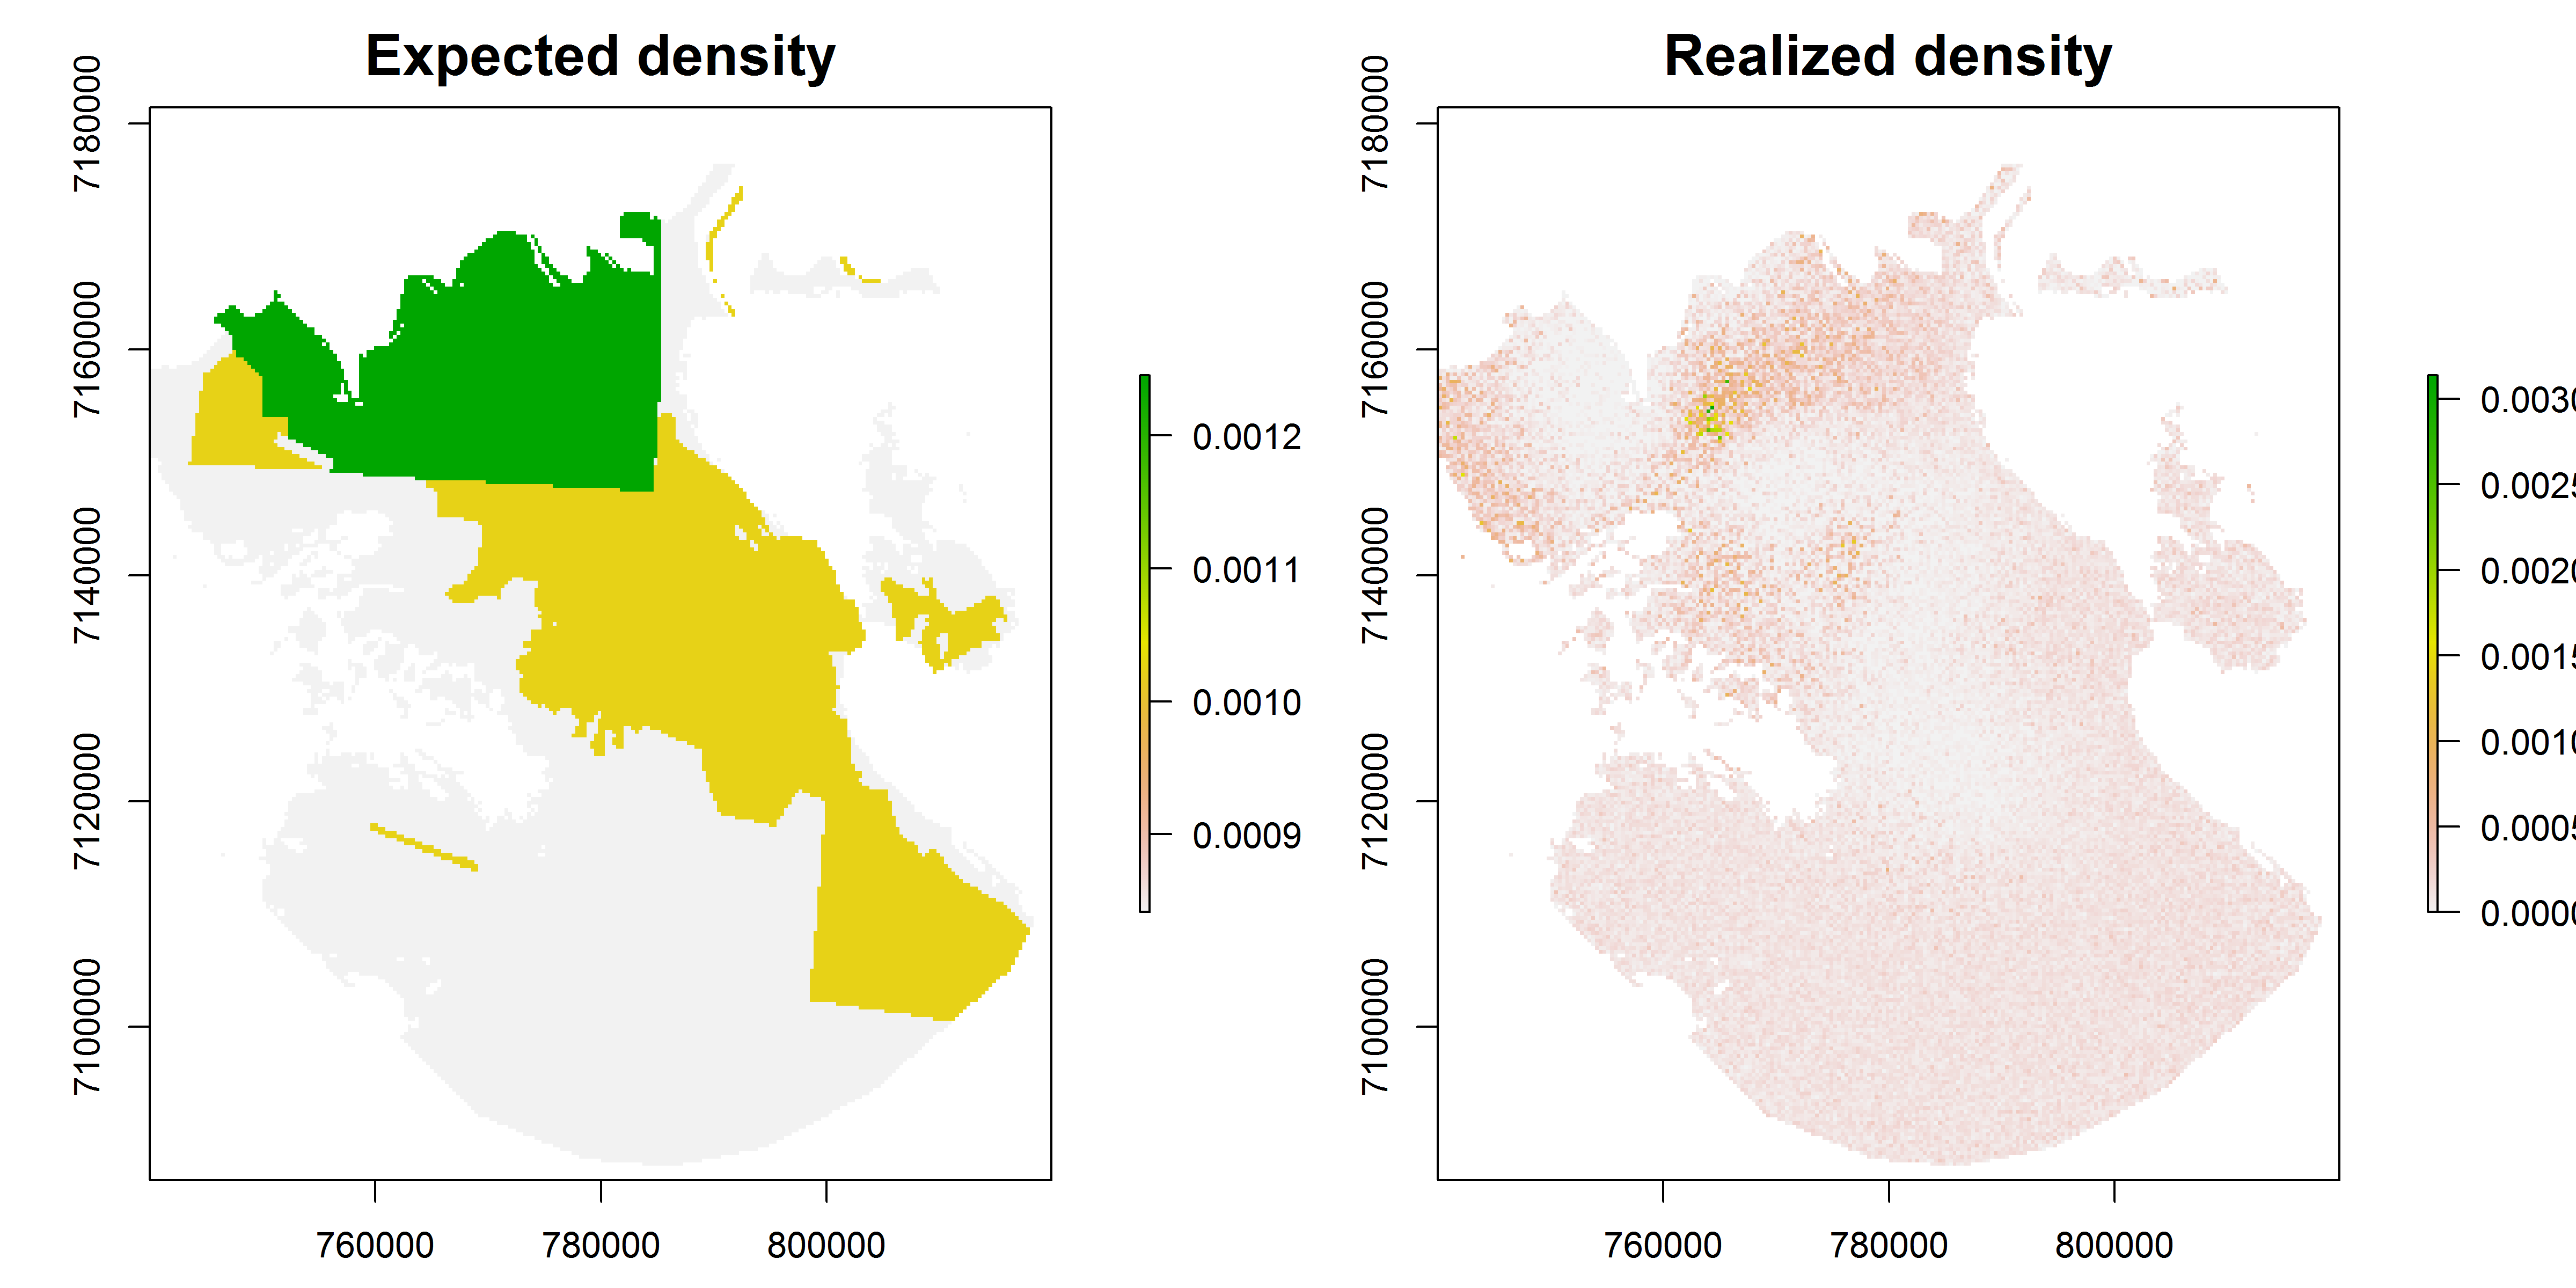
\includegraphics[width=\textwidth]{Ch13-Statespace/figs/reD}
\label{state-space.fig.Dsurface}
\caption{Estimated density surfaces from the analysis of the jaguar data.}
\end{figure}

We note that there is room for improvement in our analysis and our
results should be considered preliminary. The
political boundaries used to demarcate protected areas are not as
concrete as we might like. In reality poaching pressure is likely
higher near remote park boundaries than in well-guarded park
interiors. One option for addressing this would be to use a continuous
measure of poaching pressure such as distance from the nearest town,
or some other accessibility metric. It would also be interesting to
model density separately for each sex. Many of the detections outside
of the park were of males, and thus it is possible that the sexes use
habitat differently \citep{conde_etal:2010}. Other extensions worth
investigation include treating PROTECT as a categorical, rather than
ordinal, variable; and, it would interesting to assess the effects of
roads and trails on jaguar movement using the methods described in
Chapt.~\ref{chapt-ecoldist}. Developing models for these extensions
could be readily accomplished by modifying the fitting functions found
in the \R~package \scrbook.



\section{Summary and Outlook}

One of the distinguishing features of spatial capture-recapture models
is that they allow for inference about spatial variation
in density without relying on ad hoc approaches for determining the
amount of area surveyed. The approach described
in this chapter involves modeling the locations of activity centers as outcomes
of an inhomogeneous point process with intensity determined by
covariates defined at all locations in the state-space. Covariate
effects can be evaluated in exactly the same way as is done in
generalized linear models, making it easy to interpret the results.

All the examples in this section included a single state-space
covariate, but this was for simplicity only. Including multiple
covariates poses no additional challenges. Similarly, additional model
structure such sex-specific encounter rate parameters or behavioral
responses can be accommodated and fit using \secr, \bugs, or by
extending the functions in \scrbook. It is also possible to consider
covariates that affect both density and ecological
distance. The ramifications of this are enormous for applied
ecological research and conservation efforts because %, for instance,
researchers can use capture-recapture data to identify areas where
both density and landscape connectivity are high
\citep{royle_etal:2012ecol}. Addressing such questions
is simply not possible using standard, non-spatial capture-recapture
methods. %Accomplishing these goals will of course require more data
%than is needed to estimate the parameters of a basic SCR model.

% When maximum likelihood is used,
% it is convenient to replacing the uniform prior on
% the activity centers with a prior based on the point process intensity
% function of covariates. This distribution has been widely used in
% ecology to model point processes as well as resource selection
% probability functions \citep{manly_etal:2002,lele_keim:2006}. In the SCR
% context, use of this new prior results in
% a model for the inhomogeneous point process describing the
% location of activity centers, which can be used to test hypotheses
% about spatial variation in density. In
% rare cases, these covariates are truly continuous in the sense that
% they are defined as a function of space. More often, covariates are
% represented as rasters, which simplifies the analysis. Fitting these
% models can be accomplished using \bugs, \secr, or the custom \R~code
% presented in this chapter and found in the package \scrbook.
% %However,
% %at the time this book was written, \scrbook is only software available
% %for fitting models with covariates of both density and ecological
% %distance.

Although we focused on modeling the point process intensity as a
function of covariates, other options for fitting inhomogeneous model
exist \citet{illian_etal:2008}. Cox processes are  models in which the
intensity parameter is a function of spatial random effects. Such
methods are useful for accommodating overdispersion, but it seems unlikely that
most SCR datasets could support such complexity. Gibbs processes
are another important class of models that are distinguished by the
interactions of points. Although little work has been done on such
models in the context of SCR studies \citep{reich_etal:2012}, we
expect they will receive more
attention because they can be used to model processes such
territoriality (points repel one another) or aggregation (points
attract one another). Neyman-Scott processes are another option for
modeling aggregation or clustering, and could be useful for studying
gregarious species.



\chapter{
%Modeling Animal space-usage with
%Detection Models based on Ecological Distance
%Ecological Distance Models in Spatial Capture-Recapture
Modeling Landscape Connectivity
}
\markboth{Ecological Distance}{}
\label{chapt.ecoldist}


\vspace{.3in}


Every spatial capture-recapture model that we have considered so far
has expressed encounter probability as function of the Euclidean
distance between individual activity centers ${\bf s}$ and trap
locations ${\bf x}$.  As a practical matter, models based on Euclidean
distance imply circular, symmetric, and stationary home ranges of
individuals, and these are not often biologically realistic.  While
these simple encounter probability models will often be sufficient for
practical purposes, especially in small data sets, sometimes
developing more complex models of the detection process as it relates
to space usage of individuals will be useful.  Animals may not judge
distance in terms of Euclidean distance but, rather, according to
the configuration of habitat patches, quality of local habitat, %landscape connectivity,
perceived mortality
risk, and other considerations. % affecting movement behavior.
Together, the degree to which these factors facilitate or impede
movement determines landscape connectivity
\citep{tischendorf_fahrig:2000}, which is widely recognized to be an
important component of population viability
\citep{with_crist:1995,compton_etal:2007}.
Moreover, because encounter probability and the distance metric upon which it is
based represent outcomes of individual movements about their home
range, ecologists might have explicit hypotheses about how
environmental variables affect the distance metric, and it is
therefore desirable to incorporate these hypotheses directly into SCR
models so that they may be formally evaluated statistically.

%Assessing the impacts of habitat fragmentation and habitat loss on
%population density and landscape connectivity are high priorities in
%applied ecological research.  %Landscape connectivity is defined as the
%degree to which landscape structure impedes or facilitates movement
%\citep{tischendorf_fahrig:2000} and is widely recognized to be an
%important component of population viability
%\citep{with_crist:1995}.
Although much theory has been developed to
predict the effects of decreasing connectivity, few empirical studies
have been conducted to test these predictions due to the paucity of
formal methods for estimating connectivity parameters
\citep{cushman_etal:2010}. Instead, ecologists often rely on expert
opinion or \textit{ad hoc} methods of specifying connectivity values,
even in important applied settings
\citep{adriaensen_etal:2003,beier_etal:2008,zeller_etal:2012}. In
addition, no methods are available for simultaneously estimating
population density and connectivity parameters, in spite of theory
predicting interacting effects of density and connectivity on
population viability \citep{tischendorf_etal:2005,cushman_etal:2010}.
In this chapter, following \citet{royle_etal:2012ecol}, we provide a
framework for modeling landscape connectivity using SCR models, by
parameterizing models for encounter probability based on ``ecological
distance''.  A natural candidate framework for modeling ecological
distance is the least-cost path which is used widely in landscape
ecology for modeling connectivity, movement and gene flow
\citep{adriaensen_etal:2003,manel_etal:2003,mcrae_etal:2008}.  In
practical applications, variables that influence landscape
connectivity, or the effective cost of moving across the landscape,
include things like highways \citep[e.g.,][]{epps_etal:2005},
elevation \citep{cushman_etal:2006}, ruggedness
\citep{epps_etal:2007}, snow cover \citep{schwartz_etal:2009},
distance to escape terrain \citep{shirk_etal:2010}, range limitations
\citep{mcrae_beier:2007}, or distance from urban areas, highways,
human disturbance or other factors that animals might avoid.


\citet{royle_etal:2012ecol} provided an SCR
framework based on least-cost path for modeling landscape
connectivity. They parameterized encounter probability
based not on Euclidean distance but, rather,
on the least-cost path between an individual's activity center and a
trap location. This is parameterized in terms of one or more
parameters that relate the {\it resistance} of the landscape to
explicit covariates.  In this way, SCR models can explicitly accommodate
landscape structure and account for connectivity of the landscape.
%For these models based on least-cost path, it is convenient to use a
%likelihood-based inference framework which we follow here in this
%chapter.
Using this
methodological extension of SCR models, it is possible to make formal
statistical inferences about movement and connectivity from
capture-recapture studies that generate sparse individual encounter
history data without subjective prescription of resistance or cost
surfaces. %, which is commonly done in practice. XXXX already said
While we believe there
should be much ecological interest in developing SCR models that
account for landscape connectivity, it is also important for obtaining
more accurate estimates of density; under simple models of landscape
connectivity, incorrectly fitting the basic model SCR0 produces
substantial bias in estimates of $N$ and hence density  \citep{royle_etal:2012ecol}.


\section{Shortcomings of Euclidean Distance Models}

In the standard SCR models, encounter probability is modeled as a
function of Euclidean distance. For example, using the binomial
observation model (Chapt. \ref{chapt.scr0}), let $y_{ij}$ be
individual- and trap-specific binomial counts with sample size $K$ and
probabilities $p_{ij}$. The Gaussian model is
\[
p_{ij} = p_{0} \exp(-  d_{ij}^2 /(2\sigma^{2}) )
\]
where $d_{ij} = ||{\bf x}_{j} - {\bf s}_{i}||$ is Euclidean
distance. As usual, we will sometimes adopt the log-scale
parameterization based on $\log(p_{ij})= \alpha_{0} + \alpha_{1}
d_{ij}^{2}$ where where $\alpha_{0} = \log(p_{0})$ and $\alpha_{1} =
-1/(2\sigma^2)$.

The main problem with the Euclidean distance metric in this encounter
probability model is that it is unaffected by habitat or landscape
structure, and it implies that the space used by individuals is
stationary and symmetric, which may be unreasonable assumptions for
some species. By stationary %here
we mean in the formal sense of
invariance to translation. That is, the properties of an individual
home range centered at some point ${\bf s}$ are exactly the same as
any other point say ${\bf s}'$.  As an example, if the common
detection model based on a bivariate normal probability distribution
function is used, then the implied space usage by {\it all}
individuals, no matter their location in space or local habitat
conditions, is symmetric with circular contours of usage intensity.

In the framework of \citet{royle_etal:2012ecol}, SCR models explicitly
incorporate information about the landscape so that a unit of distance
is variable depending on identified covariates, say
$C({\bf x})$. %$z({\bf x})$.
Thus, where an individual lives on the landscape, and the state of the
surrounding landscape, will determine the character of its usage of
space. In particular, they suggest distance metrics, based on
least-cost path, that imply irregular, asymmetric and non-stationary
home ranges of individuals. As an example, Fig. \ref{fig.distort}
shows a typical symmetric home range (left panel), and a compressed
home range (right panel) resulting from the effect of an environmental
variable (center panel) on an animal's movement behavior. We might
think of the environmental variable as representing an elevation
gradient of a valley and so, for a species that avoids high elevation,
space usage will be concentrated in flatter terrain at lower
elevations and therefore producing the elliptical home range shape.
%We reproduce the application from \citet{royle_etal:2012ecol} later in
%this chapter, in addition to providing an alternative applied context
%that involves computing distances within odd-shaped landscape patches
%(Sec. \ref{ecoldist.sec.buffer}).


\begin{figure}[h]
\centering
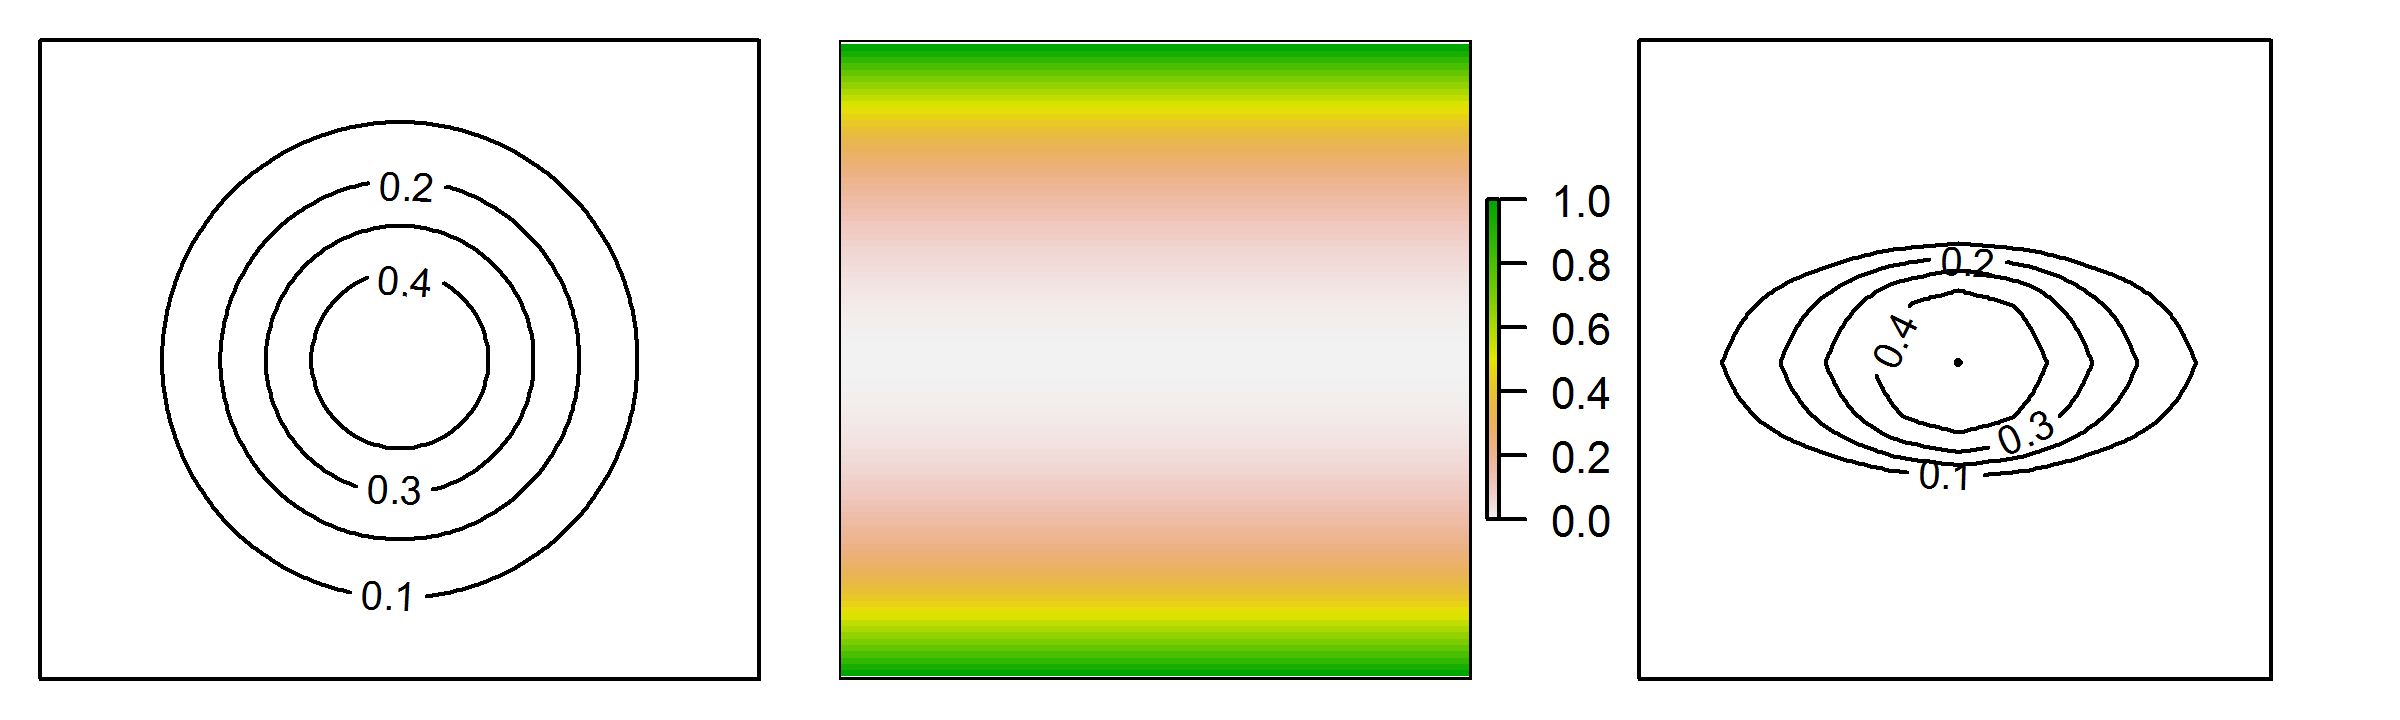
\includegraphics[width=5in,height=1.3in]{Ch12-EcolDist/figs/distort}
\caption{A symmetric home range (left), a habitat variable (center)
  such as representing an elevation gradient,
  and a non-symmetric home range (right) resulting from the cost imposed on
  movement by the habitat variable.}
\label{fig.distort}
\end{figure}


\section{Least-Cost Path Distance}

We adopt a cost-weighted distance metric here which defines the
effective distance between points by accumulating pixel-specific costs
determined using a cost function defined by the user.  The idea of
cost-weighted distance to characterize animal use of landscapes is
widely used in landscape ecology for modeling connectivity, movement
and gene flow \citep{beier_etal:2008}. For reasons of computational
tractability we consider a discrete landscape defined by a raster of
some prescribed resolution. The distance between any two points ${\bf
  x}$ and ${\bf x}'$ can be represented by a sequence of line segments
connecting neighboring pixels, say ${\bf l}_{1},{\bf
  l}_{2},\ldots,{\bf l}_{m}$. Then the cost-weighted distance between
${\bf x}$ and ${\bf x}'$ is
\begin{equation}
 d({\bf x},{\bf x}')
  =  \sum_{i=1}^{m-1} \mbox{cost}({\bf l}_{i},{\bf l}_{i+1})||{\bf l}_{i} - {\bf l}_{i+1}||
\label{eq.costweighted}
\end{equation}
where $\mbox{cost}({\bf l}_{i},{\bf l}_{i+1})$ is the user-defined cost to
move from pixel ${\bf l}_{i}$ to neighboring pixel ${\bf l}_{i+1}$ in
the sequence.  Given the cost of each pixel, it is a simple matter to
compute the cost-weighted distance between any two pixels, along {\it
  any} path, simply by accumulating the incremental costs weighted by
distances.  In the context of spatial capture-recapture models (and,
more generally, landscape connectivity) we are concerned with the {\it
  minimum} cost-weighted distance, or the {\it least-cost path},
between any two points which we will denote by $d_{lcp}$, which is the
sequence ${\cal P} = ({\bf l}_{1},{\bf l}_{2},\ldots,{\bf l}_{m})$
that minimizes the objective function defined by
Eq. \ref{eq.costweighted}. That is,
\begin{equation}
 d_{lcp}({\bf x},{\bf x}')
  =  \min_{{\cal P}} \sum_{i=1}^{m-1} \mbox{cost}({\bf l}_{i},{\bf l}_{i+1})||{\bf l}_{i} - {\bf l}_{i+1}||
\label{eq.lcp}
\end{equation}
The least-cost path distance can be calculated in
 many geographic information systems and other software packages,
including the {\bf R} package \mbox{\tt
  gdistance} \citep{vanetten:2011} which we use below.

The key ecological aspect of least-cost path modeling is the
development
of models for pixel-specific cost.
%In this paper we
A natural approach is to
model cost as a function of one or more covariates
defined on every pixel of the according raster. For example, using a
single covariate $C({\bf x})$ we define the cost of moving from some pixel
${\bf x}$ to neighboring pixel ${\bf x}'$ as
\begin{equation}
\log(  cost({\bf x},{\bf x}'))=  \alpha_{2}\left( \frac{C({\bf
      x})+C({\bf x}')}{2}
\right)
\label{ecoldist.eq.cost}
\end{equation}
Thus, if $\alpha_{2} = 0$ then substituting $\mbox{cost}({\bf x},{\bf x}')
=\exp(0) = 1$ into
Eq. \ref{eq.lcp} will produce the ordinary Euclidean distance
between points. Here we assume the covariate $C$ is positive-valued,
and we constrain $\alpha_{2}\ge 0$ so as to avoid
negative costs. While not necessarily problematic from a mathematical
standpoint, negative costs are unrealistic biologically.

The use of least-cost path models to model landscape connectivity has
been around for a long time. And, although $\alpha_{2}$ is rarely
known, conservation biologists design linkages that require this
resistance value as input \citep[see][and articles cited
therein]{beier_etal:2008}.  However, formal inference (e.g.,
estimation) of parameters is not often done.  Instead, in many
existing applications of least-cost path analysis, the parameter
$\alpha_{2}$ is fixed by the investigator, or based on expert opinion
\citep{beier_etal:2008}, although recently researchers have begun to
define costs based on resource selection functions\footnote{We address the integration of resource
selection models based on telemetry data with SCR models in
Chapt. \ref{chapt.rsf}.},
animal movement
\citep{tracy:2006, fortin_etal:2005}, or genetic distance data (e.g.,
\citet{gerlach_musolf:2000}; \citet{epps_etal:2007};
\citet{schwartz_etal:2009}.


To formalize the use of cost-weighted distance in SCR models, we
substitute Eq. \ref{eq.lcp} in the expression for encounter
probability (Eq. \ref{eq.encounter}) and maximize the resulting
likelihood (see  below). In doing so, we can directly
estimate parameters of the least-cost path model, evaluate how
landscape covariate influence connectivity, and test explicit hypotheses
about these things using only individual level encounter history data
from capture-recapture studies.


\subsection{Example of Computing Cost-weighted distance}

As an example of the cost-weighted distance calculation consider the
following landscape comprised of 16 pixels with unit spacing
identified as follows, along with the pixel-specific cost:
\begin{center}
\begin{verbatim}
      pixel ID                 Cost
     4 8 12 16            100   1   1  1
     3 7 11 15            100 100   1  1
     2 6 10 14            100 100 100  1
     1 5  9 13            100 100   1  1
\end{verbatim}
\end{center}
We assume the scale is such that the distance between neighboring
pixels in any cardinal direction is 1 unit, and the distance between
neighbors on a diagonal is $\sqrt{2}$ units.  We assigned low cost of
1 to ``good habitat'' pixels (or pixels we think of as ``highly
connected'' by virtue of being in good habitat) and, conversely, we
assign high cost (100) to ``bad habitat''.  This simple cost raster is
shown in Fig. \ref{ecoldist.fig.raster}.  The {\bf R} commands for
creating this simple example are as follows (which can be run using
the {\bf R} script \mbox{\tt SCRed} -- see the help file for that):
\begin{verbatim}
> library(raster)
> library(gdistance)
> r<-raster(nrows=4,ncols=4)
> projection(r)<- "+proj=utm +zone=12 +datum=WGS84" # Sets the projection
> extent(r)<-c(.5,4.5,.5,4.5) #sets the extent of the raster
> costs1<- c(100,100,100,100,1,100,100,100,1,1,100,1,1,1,1,1)
> values(r)<-matrix(costs1,4,4,byrow=FALSE) #assign the costs to the raster
> par(mfrow=c(1,1))
> plot(r)
\end{verbatim}
This produces Fig. \ref{ecoldist.fig.raster}.

\begin{figure}[h]
\begin{center}
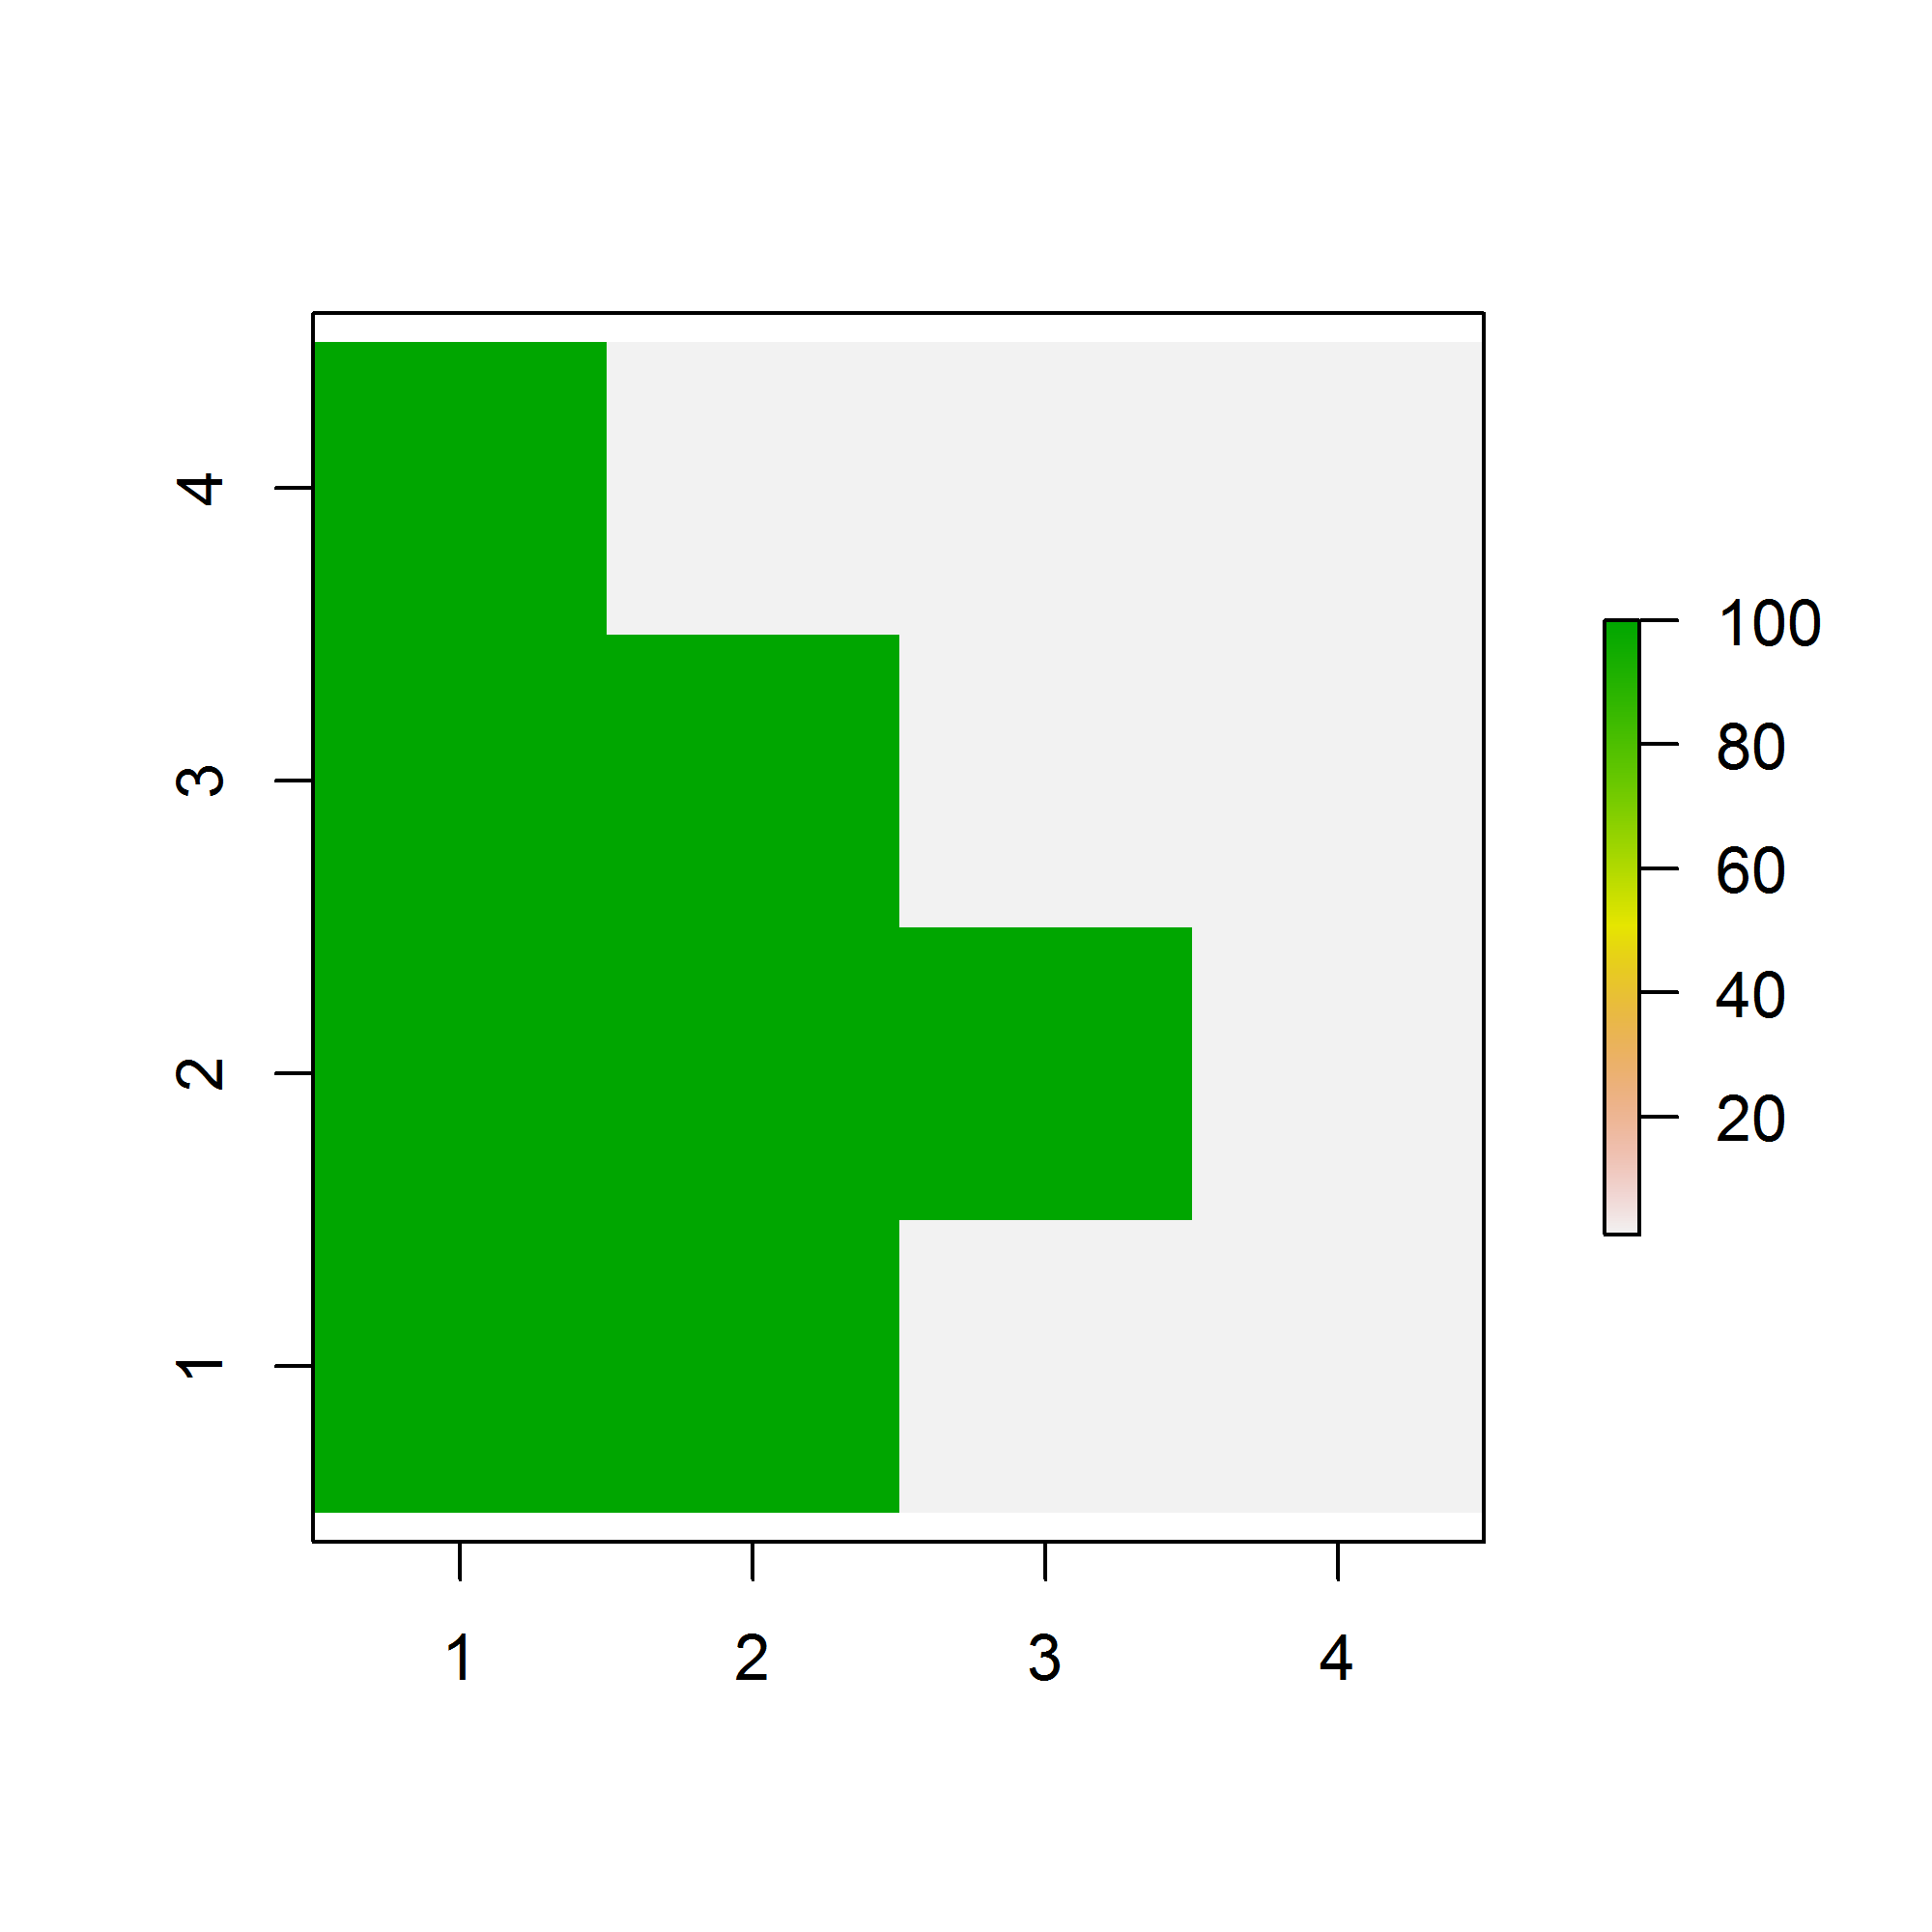
\includegraphics[height=3.25in,width=3.25in]{Ch12-EcolDist/figs/raster_2values}
\end{center}
\caption{A $4 \times 4$ raster depicting a binary cost surface, with cost = 1 (white) or 100 (shaded) to represent ease of movement across a pixel.}
\label{ecoldist.fig.raster}
\end{figure}

For this simple case we
 can easily compute the shortest cost-weighted distance between any
pixels ``by eye''.  For example, the shortest cost-weighted distance between
pixels 5 and 9 in this example is 50.5 units: $1*(100+1)/2 = 50.5$,
the shortest distance between pixels 4 and 8 is also 50.5, while the
shortest cost-distance between 4 and 12 is 51.5.  What is the shortest
distance between 7 and 16? Suppose an individual at pixel 7 can move
diagonal (which has distance $\sqrt{2}$) and pay $\sqrt{2}(100+1)/2$,
and then move once to the right to pay $1$ additional unit cost, for a
total of $72.4$. However, if the individual instead moved one unit to
the right, to pixel 11, and then diagonally, the total cost is
$51.914$ which is the minimum cost-weighted distance in getting from
pixel 7 to 16. These two ways of moving from 7 to 16 have the same
Euclidean distance, but different cost-weighted distances according to
our cost function.

The least-cost path distances can be
computed with just a couple {\bf R} commands, and these commands can
be inserted directly into the likelihood construction for an ordinary
spatial capture-recapture model. The {\bf R} package
\mbox{\tt gdistance} calculates least-cost path using  Dijkstra's algorithm
\citep{dijkstra:1959} (from the \mbox{\tt igraph} package
\citep{csardi:2010}).
%Using \mbox{\tt gdistance}, we
%define the incremental cost of moving from one pixel to another as the
%distance-weighted {\it average} of the 2 pixel costs. We demonstrate
%how to do this subsequently.
To compute the least-cost path, or the minimum cost-weighted distances
between every pixel and every other pixel, we make use of the helper
function \mbox{\tt transition}, which calculates the cost of moving
between neighboring pixels.  It operates on the inverse-scale
(``conductance''), and so the \mbox{\tt transitionFunction} argument
is given as $1/mean(x)$.  The function \mbox{\tt geoCorrection}
modifies this object depending on the projection of the coordinate
system (e.g., it corrects for curvature of the earth's surface if
longitude/latitude coordinates are used).  The result is fed into the
function \mbox{\tt costDistance} to compute the pair-wise distance
matrix. For that, we define the center points of each raster, here
these are just integers on $[1,4] \times [1,4]$.  The commands
altogether are as follows: {\small
\begin{verbatim}
> tr1<-transition(r,transitionFunction=function(x) 1/mean(x),directions=8)
> tr1CorrC<-geoCorrection(tr1,type="c",multpl=FALSE,scl=FALSE)
> pts<-cbind( sort(rep(1:4,4)),rep(4:1,4))
> costs1<-costDistance(tr1CorrC,pts)
> outD<-as.matrix(costs1)
\end{verbatim}
}
Now we can look at the result and see if it makes sense to us. Here we
produce the first 5 columns of this distance matrix to illustrate a
couple of examples of calculating the minimum cost-weighted distance
between points:
\begin{center}
{\small
\begin{verbatim}
> outD[1:5,1:5]
         1        2        3        4        5
1   0.0000 100.0000 200.0000 205.2426 100.0000
2 100.0000   0.0000 100.0000 200.0000 141.4214
3 200.0000 100.0000   0.0000 100.0000 126.1604
4 205.2426 200.0000 100.0000   0.0000 105.2426
5 100.0000 141.4214 126.1604 105.2426   0.0000
\end{verbatim}
}
\end{center}
An interesting case is that between point 1 and 4. Note that simply
taking the shortest Euclidean distance, weighted by cost, produces a
cost-weighted distance of $100 \times 1$ to move from pixel 1 to pixel
2, and similarly from 2 to 3 and 3 to 4, producing a total
cost-weighted distance of $300$. However, the actual {\it least-cost
  path} has cost-weighted distance $205.2426$. See if you can figure
out the shortest path by inspection.

The key point here is that, once we can compute this distance matrix,
we can use it as the distance matrix in computing the encounter
probability between acctivity centers and traps, and we can use our
existing MLE technology (Chapt. \ref{chapt.mle}) to fit models that
are based on ecological distance.



\section{Simulating SCR Data using Ecological Distance}
\label{ecoldist.sec.simulating}

\citet{royle_etal:2012ecol} simulated capture-recapture data
%in the presence of
such that landscape connectivity was governed by %using
a cost function having a
single covariate, and they considered two hypothetical covariate
landscapes
(Fig. \ref{ecoldist.fig.raster100}).
%typical of how
%cost-weighted distance models might be used in real capture-recapture
%problems.
The landscape here is a $20 \times 20$ pixel raster, with
extent = $[0.5, 4.5] \times [0.5, 4.5]$.
For example, think of each pixel as
representing, say, a $1 \times 1$ km grid cell with something like
``percent developed'' or ``trail/road density'' representing the
covariate. For sampling by capture-recapture, imagine
that 16 camera traps are established at the integer coordinates
$(1,1), (1,2), \ldots, (4,4)$.
The two covariates were constructed as follows (see \mbox{\tt
  ?make.EDcovariates} for the {\bf R} commands):
First is an increasing trend from
the NW to the SE (``systematic covariate''), where $C({\bf x})$ is defined as
$C({\bf x}) = row({\bf x}) + col({\bf x})$ and $row({\bf x})$ and $col({\bf x})$ are just the row and
column, respectively, of the raster.  This might mimic something
related to distance from an urban area or a gradient in habitat
quality due to land use, or environmental conditions such as
temperature or precipitation gradients.  In the second case we make up
a covariate by generating a field of spatially correlated noise to
emulate a typical patchy habitat covariate (``patchy covariate'') such as
tree or understory density.

For both covariates we use a
cost function in which transitions from pixel ${\bf x}$ to ${\bf x}'$
is given by:
\[
 \log(\mbox{cost}({\bf x},{\bf x}'))=  \alpha_2 \left( \frac{C({\bf
       x}) + C({\bf x}')}{2} \right)
\]
where $\alpha_2 = 1$ for simulating the observed data.
 Remember that with $\alpha_2=0$ the
model reduces to one in which the cost of moving across each pixel is
constant, and therefore Euclidean distance is operative.
In the left panel of
Fig. \ref{ecoldist.fig.raster100}, a sample realization of
$N=100$ activity centers is shown. While encounter probability is
assumed to be related to landscape connectivity according to the
single-variable cost function, individual activity centers are
assumed to be uniformly distributed, although we can modify this
assumption (See Sec.~\ref{chapt.ecoldist.sec.ssed} below).


\begin{figure}[h]
\begin{tabular}{ll}
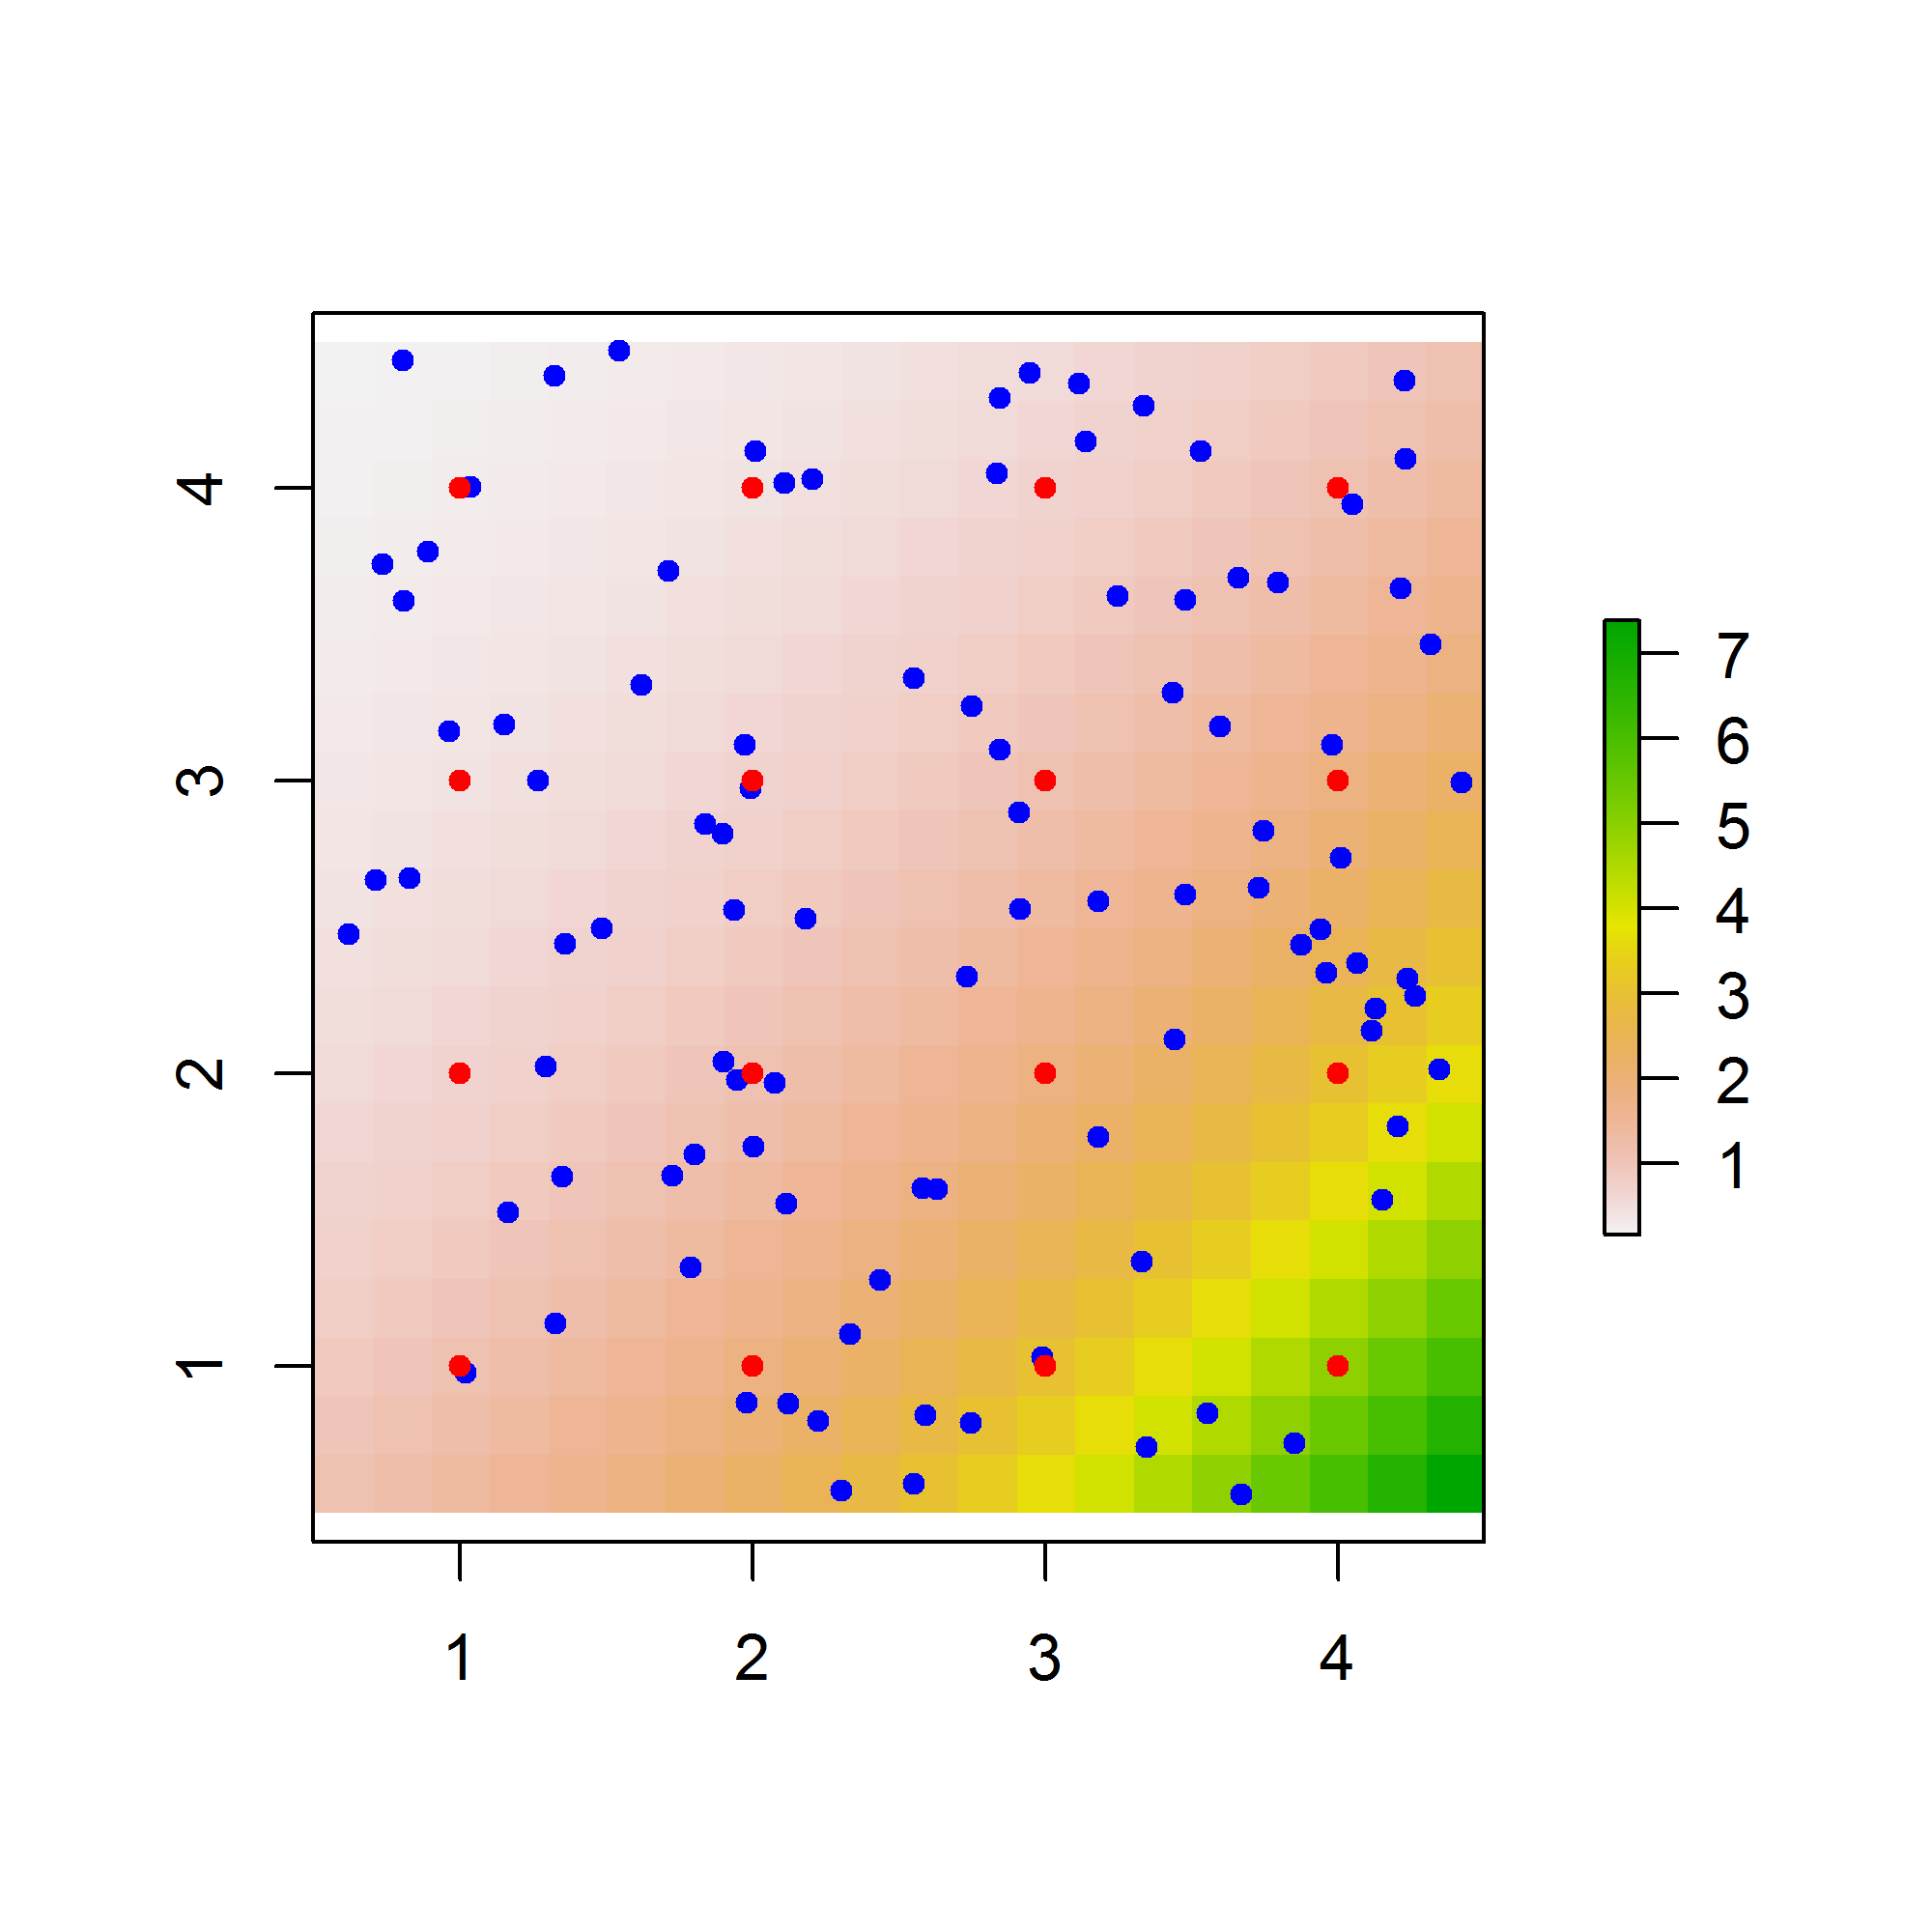
\includegraphics[height=2.5in,width=2.5in]{Ch12-EcolDist/figs/raster_withN100}
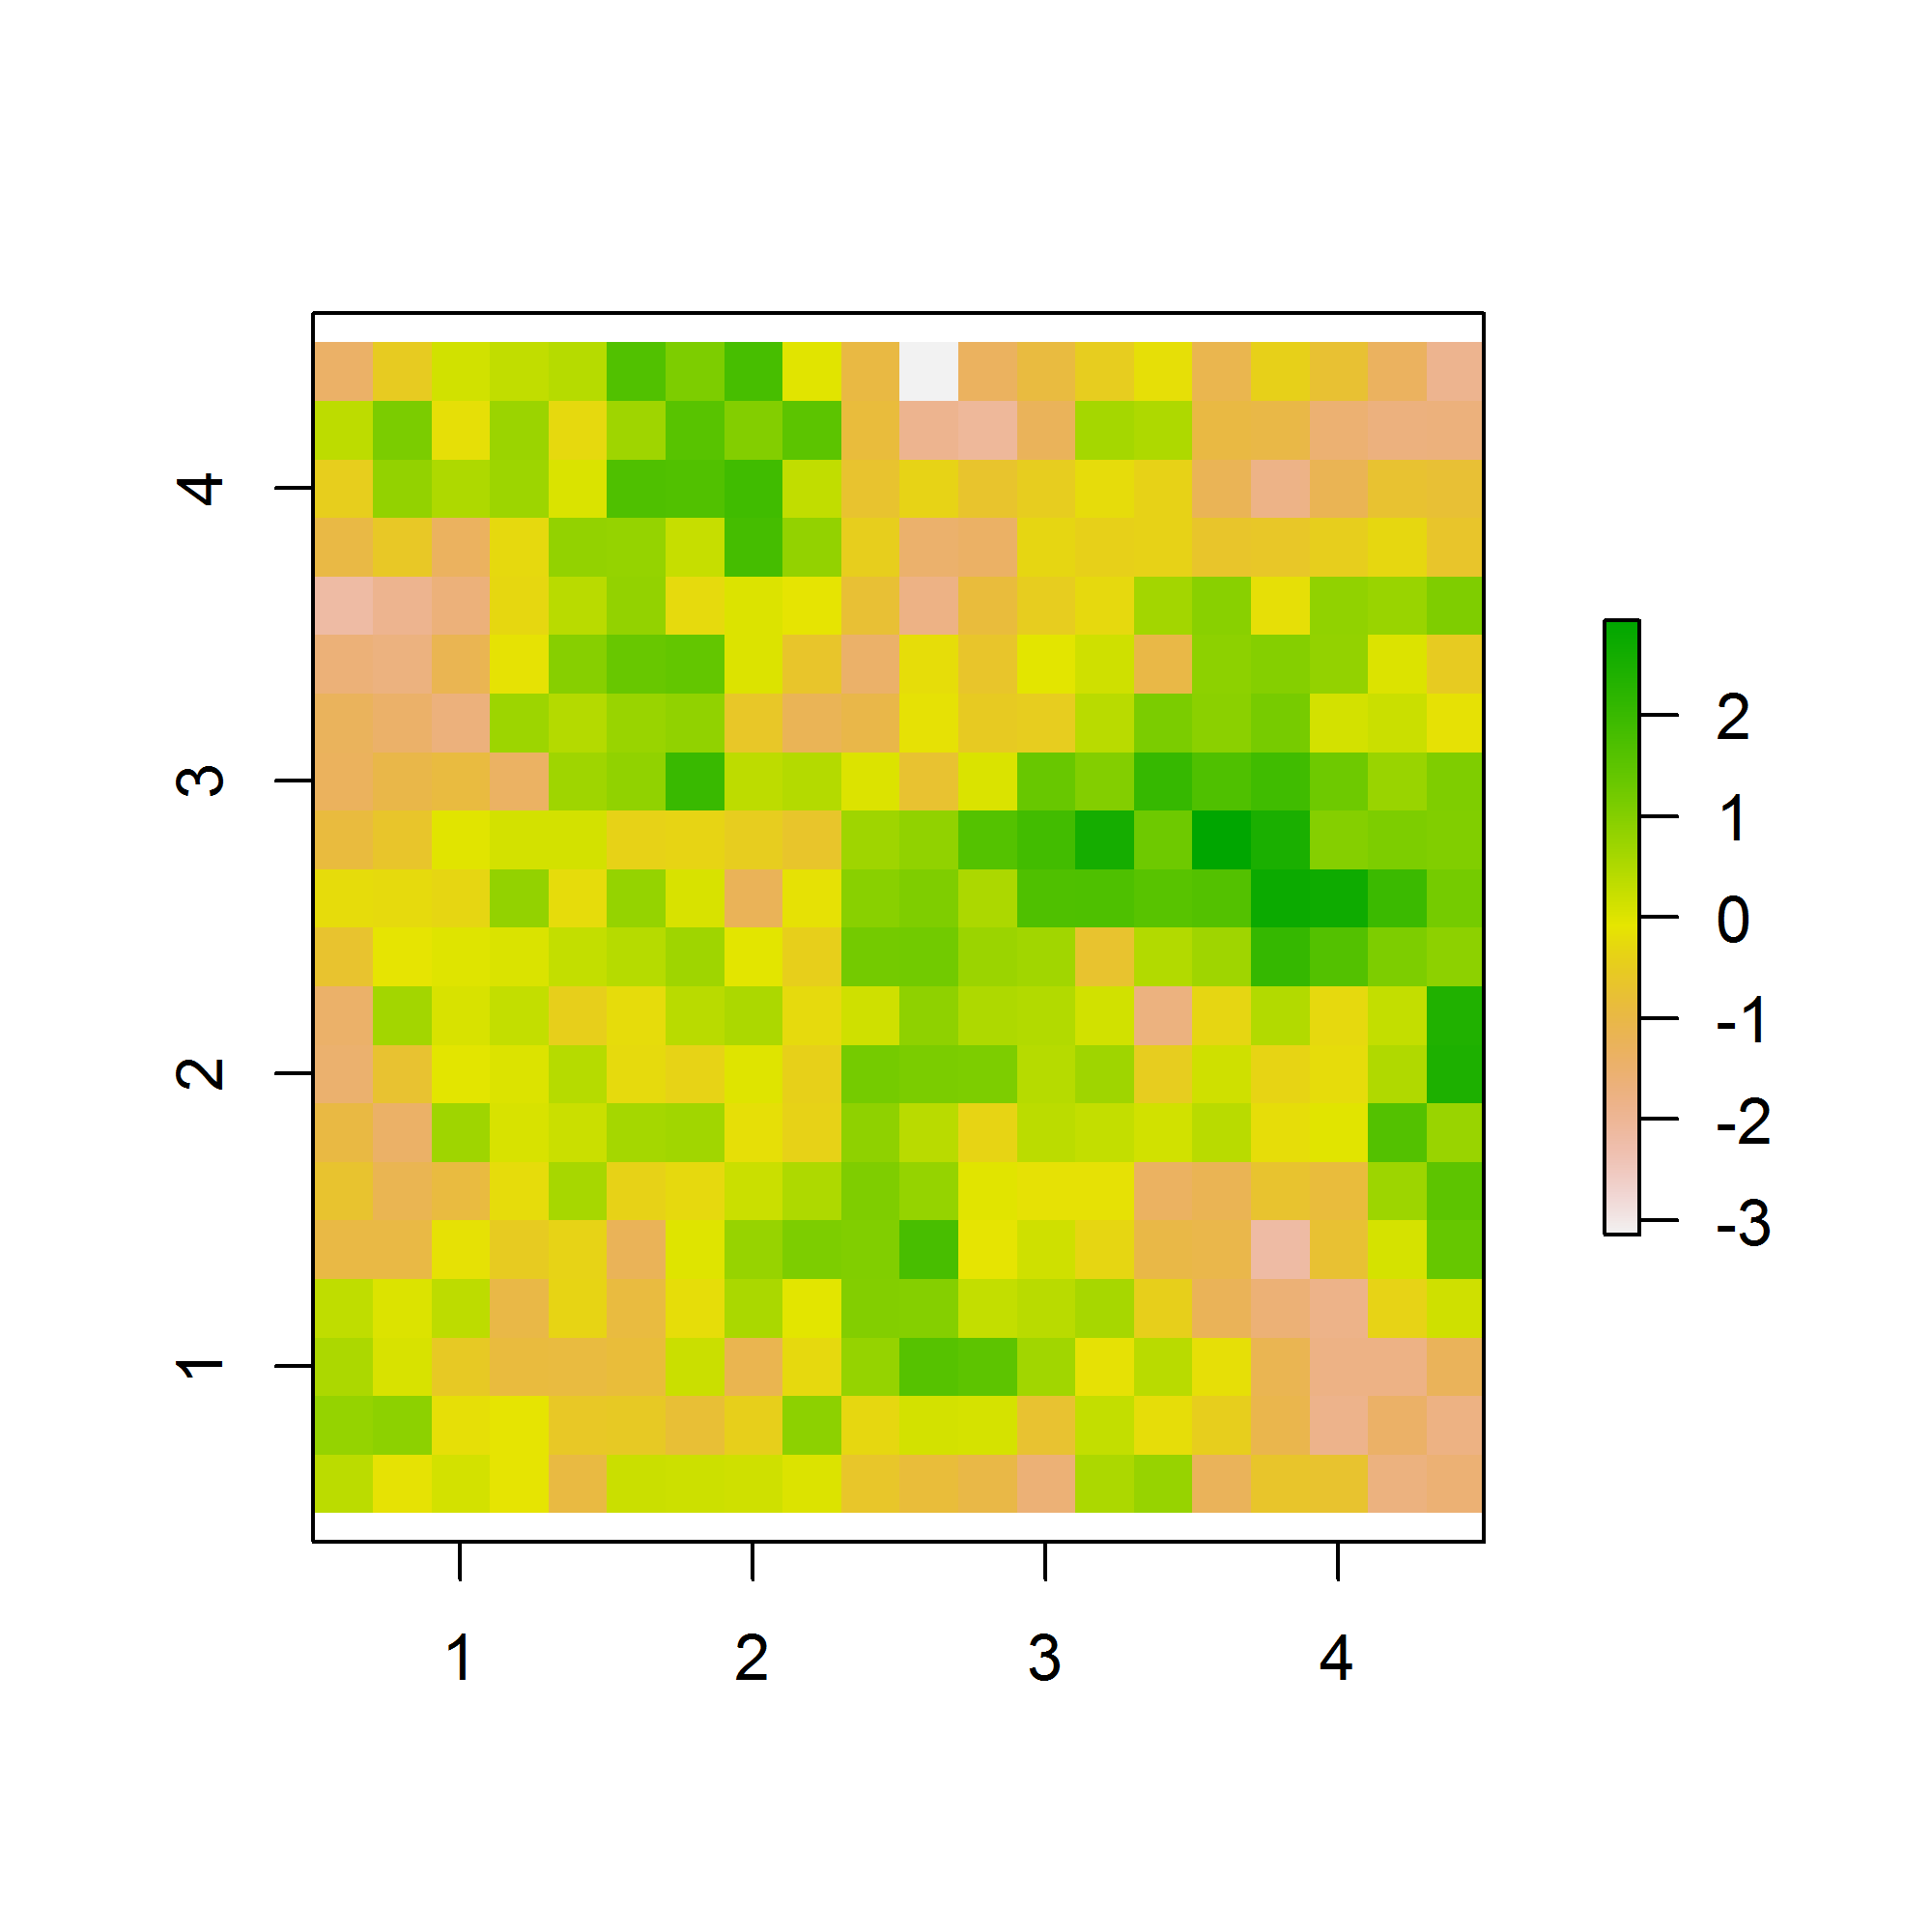
\includegraphics[height=2.5in,width=2.5in]{Ch12-EcolDist/figs/raster_krige} &
\end{tabular}
\caption{Two covariates (defined on a $20 \times 20$ grid) used in simulations.
 Left panel shows a covariate with systematic structure meant
to mimic distance from some feature, and the right panel shows a ``patchy'' covariate.
A hypothetical realization of $N=100$ activity centers (blue dots) is superimposed
  on the left figure, along with 16 trap locations. }
\label{ecoldist.fig.raster100}
\end{figure}


When distance is defined by the cost-weighted distance metric given
by Eq. \ref{eq.lcp} then individual space-usage varies
spatially in response to the landscape covariate(s) used in the
distance metric.  As a consequence, home range contours are no longer
circular, as in SCR models based on Euclidean distance.
For example, using one of the covariates we use in
our simulation study below (Fig. \ref{ecoldist.fig.raster100}, right
panel) with a Gaussian
%pdf detection function
encounter model but having distance
metric defined by Eq. \ref{eq.lcp}, produces home ranges such
as those shown in Fig. \ref{fig.homeranges}.


\begin{figure}
\begin{center}
\includegraphics[height=6in,width=3.75in]{Ch12-EcolDist/figs/home_ranges}
\end{center}
\caption{
Typical home ranges for 6 individuals based on the cost surface shown in the right panel of
  Fig. \ref{ecoldist.fig.raster100} with $\alpha_{2}=1$. The black dot indicates the home
  range center and the pixels around each home range center are shaded
according to the probability of encounter, if a trap were located in
that pixel.
}
\label{fig.homeranges}
\end{figure}

To simulate data,
 we have to load the \mbox{\tt
scrbook} package and call the function \mbox{\tt make.EDcovariates} to generate
our raster covariates (see the help file for how that is done). We
process the covariate into a least-cost path distance
matrix, and then simulate observed encounter data using standard methods
which we have used many times previously in this book. The complete set
of {\bf R} commands is:
{\small
\begin{verbatim}
### Grab a covariate
library(scrbook)
set.seed(2013)
out<-make.EDcovariates()
covariate<-out$covariate.patchy

### prescribe some settings
N<-200
alpha0<- -2
sigma<- .5
alpha1<- 1/(2*sigma*sigma)
alpha2<-1
K<- 5
S<-cbind(runif(N,.5,4.5),runif(N,.5,4.5))

# make up some trap locations
xg<-seq(1,4,1); yg<-4:1
traplocs<-cbind( sort(rep(xg,4)),rep(yg,4))
points(traplocs,pch=20,col="red")
ntraps<-nrow(traplocs)

### make a raster and fill it up with the "cost"
r<-raster(nrows=20,ncols=20)
projection(r)<- "+proj=utm +zone=12 +datum=WGS84"
extent(r)<-c(.5,4.5,.5,4.5)
cost<- exp(alpha2*covariate)

### compute least-cost path distance
tr1<-transition(cost,transitionFunction=function(x) 1/mean(x),directions=8)
tr1CorrC<-geoCorrection(tr1,type="c",multpl=FALSE,scl=FALSE)
D<-costDistance(tr1CorrC,S,traplocs)
probcap<-plogis(alpha0)*exp(-alpha1*D*D)

# now generate the encounters of every individual in every trap
# discard uncaptured individuals
Y<-matrix(NA,nrow=N,ncol=ntraps)
for(i in 1:nrow(Y)){
 Y[i,]<-rbinom(ntraps,K,probcap[i,])
}
Y<-Y[apply(Y,1,sum)>0,]
\end{verbatim}
}


\section{Likelihood Analysis of Ecological Distance Models}
\label{ecoldist.sec.mle}

Throughout much of this book we rely on Bayesian analysis by MCMC
mostly using {\bf BUGS}, but sometimes (as in Chapt. \ref{chapt.mcmc})
developing our own implementations. However, occasionally we prefer to
use likelihood estimation, such as when we can compare a set of models
directly by likelihood either to do a direct hypothesis test of a
parameter, or to tabulate a bunch of AIC values. For the class of
models that use least-cost path, we also prefer likelihood methods not
because they have any conceptual or methodological benefit, but simply
because they are more computationally efficient to implement
\citep{royle_etal:2012ecol}.

There are no technical considerations in adapting our formulation of
maximum likelihood estimation \citep{borchers_efford:2008} from
Chapt. \ref{chapt.mle} for the class of models based on least-cost
path (see the appendix in \citet{royle_etal:2012ecol} for complete details).
Likelihood analysis is really just a straightforward adaptation in which we
replace the Euclidean distance with least-cost path.  Consider the
Bernoulli model in which the individual- and trap-specific
observations have a binomial distribution conditional on the latent
variable ${\bf s}_{i}$:
\begin{equation}
  y_{ij}| {\bf s}_{i} \sim \mbox{Binomial}(K, p_{\bm \alpha}(d_{lcp}({\bf x}_{j},{\bf s}_{i};\alpha_{2}); \alpha_{0}, \alpha_{1})
\label{ecoldist.eq.cond-on-s}
\end{equation}
where we have indicated the dependence of $p$ on the parameters
${\bm \alpha} =(\alpha_{0},\alpha_{1},\alpha_{2})$, and also $d_{lcp}$ which
itself depends on $\alpha_{2}$, and the latent variable ${\bf s}_i$.
We note that the only difference between likelihood analysis of this
model and the standard Bernoulli model, is the use of $d_{lcp}$ here.
For the random effect we have ${\bf s}_{i} \sim  \mbox{Uniform}({\cal
  S})$, we can easily compute the integrated (marginal) likelihood of
an encounter history.
The likelihood is given in the {\tt scrbook} package as the function
\mbox{\tt intlik3ed}. The help file
provides an example of its usage and for simulating data.
To use this function the cost covariate $C({\bf x})$ has to be of class
\mbox{\tt RasterLayer} which requires packages \mbox{\tt sp} and
\mbox{\tt raster} to manipulate.


\subsection{Example of SCR with least-cost path}

Now we use the {\bf R} function \mbox{\tt nlm} along with
our \mbox{\tt intlik3ed} function to  obtain the MLEs of the
model parameters for the data simulated
in Sec. \ref{ecoldist.sec.simulating}.
 We'll do that for both the standard Euclidean distance
and then for the ecological distance based on the ``patchy''
covariate using the following commands:
{\small
 \begin{verbatim}
> frog1<-nlm(intlik3ed,c(alpha0,alpha1,3)),hessian=TRUE,y=Y,K=K,X=traplocs,
               distmet="euclid",covariate=covariate,alpha2=1)

> frog2<-nlm(intlik3ed,c(alpha0,alpha1,3,-.3),hessian=TRUE,y=Y,K=K,X=traplocs,
               distmet="ecol",covariate=covariate,alpha2=NA)
\end{verbatim}
}
The summary output for the two model fits is shown in Table \ref{ecoldist.tab.results1}.
The model based on least-cost path (the data generating model) appears
to be much preferred in terms of negative log-likelihood.
The output parameter order is $(\alpha_{0}, \alpha_{1}, \log(n_{0}), \text{and}
\log(\alpha_{2}))$ (remember, we want to keep $\alpha_{2}$
positive, so it's logarithm is estimated).
The data generating parameter values were
$\alpha_{0} = - 2$,
$\alpha_{1} = 2$ and $\log(\alpha_{2}) = 0$.
The simulated sampling produced a sample of 96 individuals and so the
number of individuals not captured is
$n_{0} = 104$, and $\log(n_{0}) = 4.64$. We see that the
 MLEs of the least-cost path model are pretty close whereas they are
 not so close under the misspecified model based on Euclidean distance.



\begin{table}
\caption{
Summary output of fitting models based on Euclidean and least-cost
path distance to simulated data using the
 \mbox{\tt intlik3ed} function (see \mbox{\tt ?intlik3ed}). Data were
 simulated based on the least-cost path model using the ``patchy''
 covariate shown in Fig. \ref{ecoldist.fig.raster100}.
}
\begin{tabular}{cccccc} \hline \hline
Distance metric &  -loglik &     $\alpha_0$  & $\alpha_1$  &\mbox{log}($n_{0}$) &  $\alpha_2$ \\ \hline
True value      &          &         -2      &    2       &   4.644 & 1 \\
Euclidean   &133.495&  -1.885 &    1.247 &    3.549 &      -- \\
Least-cost path (truth) & 70.119& -1.780 &  2.471    &    4.459 &
0.046  \\ \hline
\end{tabular}
\label{ecoldist.tab.results1}
\end{table}






\section{Bayesian Analysis}

While implementation of these ecological distance SCR models is
reasonably straightforward, the model cannot be fitted
in the  {\bf BUGS} engines because least-cost path distance cannot be computed.
It would be possible to fit the models
in {\bf BUGS} if the parameter $\alpha_{2}$ was fixed. In that case,
one could compute the distance matrix ahead of time and reference the
required elements for a given ${\bf s}$.
Alternatively, it would be possible to write a custom MCMC routine
using the methods we present in Chapt. \ref{chapt.mcmc}, although we
have not yet developed our own MCMC implementation of SCR models with
ecological distance metrics.


\section{Simulation Evaluation of the MLE}

\citet{royle_etal:2012ecol}
carried-out a limited simulation study to evaluate the
general statistical performance of the density estimator under
this new model, the effect of mis-specifying the model with a
normal Euclidean distance metric, and evaluate the general bias and
precision properties of the MLE using the systematic and patchy
landscapes shown in
Fig. \ref{ecoldist.fig.raster100}.

Their results showed extreme
bias in estimates of $N$ when the misspecified Euclidean distance is
used, and only negligible small-sample
 bias of 3-5\% in the MLE of $N$ using the
least-cost distance which becomes negligible as the expected seample
size increases (either due to increasing $K$, or larger population sizes).
The performance of estimating the other parameters, including the
cost parameter $\alpha_{2}$ mirrors
the results for estimating $N$.
We reproduce a subset of the results from \citet{royle_etal:2012ecol}
%here,
in Table \ref{ecoldist.tab.simresults}.

\begin{table}[htp]
\label{tab.results1}
{\small
\caption{
Simulation results for estimating population size $N$ for a prescribed state-space with
$N=100$ or $N=200$ and various levels of replication ($K$)
using the ``patchy'' landscape shown in Fig.
 \ref{ecoldist.fig.raster100}.
For each simulated
data set, the SCR model was fitted by maximum likelihood with
standard Euclidean distance (``euclid''), or least-cost path
(``lcp''), which was the true data-generating model.
The summary statistics of the
sampling distribution reported are the mean, standard deviation
(``SD'') and quantiles (0.025, 0.50, 0.975).
}
\begin{tabular}{l|rrrrr}
  \hline
         & \multicolumn{5}{c}{N=100  }  \\ \hline
         &   mean &  SD  & 0.025 & 0.50  & 0.975   \\ \hline
$K=3$      &        &      &       &       &         \\
euclid   &  78.68 & 18.12& 49.40 & 76.34 & 125.47  \\
lcp      & 110.96 & 28.65& 69.55 &106.98 & 181.84  \\
$K=5$     &        &      &       &       &         \\
euclid   &  77.85 & 11.55& 59.17 & 77.44 & 101.14  \\
lcp      & 104.44 & 15.79& 78.38 &101.47 & 139.55  \\
$K=10$     &        &      &       &       &         \\
euclid   &  78.01 & 5.26 & 68.00 & 77.96 & 87.81   \\
lcp      & 100.42 & 7.56 & 86.72 &100.34 & 115.47  \\ \hline
        & \multicolumn{5}{c}{N=200   }  \\ \hline
$K=3$      &        &      &       &       &         \\
euclid  154.34& 33.74& 107.00& 146.34& 221.43\\
lcp     208.77& 49.29& 141.68& 197.89& 325.77\\
$K=5$           &      &       &       &        \\
euclid   153.39& 15.57& 129.31& 149.54& 185.38\\
lcp      200.91& 20.78& 164.42& 200.47& 246.46\\
$K=10$           &      &       &       &       \\
euclid   156.27&  8.51& 142.17& 156.05& 174.55\\
lcp      198.45& 11.44& 180.06& 198.04& 219.52\\ \hline
\end{tabular}
}
\label{ecoldist.tab.simresults}
\end{table}














\begin{comment}
For population sizes of 100 and 200, individuals with activity
centers randomly distributed on the $20 \times 20$ landscape, they
subjected individuals
to encounter by 16 traps arranged in a $4\times 4$ grid
using a Gaussian
encounter model with least-cost path distance metric:
\[
\log(p_{ij})= \alpha_{0} + \alpha_{1} d_{lcp}({\bf x}_{j},{\bf
  s}_{i}; \alpha_{2})^{2}
\]
where  $\alpha_{0} = -2$ and $\alpha_{1} = 2$, the latter value
corresponding to $\sigma = 0.5$ of a stationary bivariate normal home
range model.  Different numbers of replicate samples were considered,
$K=3,5,10$
(e.g., nights in a camera trapping study), in order
to produce varying sample
sizes.
For each of the ``systematic'' and ``patchy'' landscapes defined
previously, 200 data sets were simulated and, for each of those, two
different models were fitted: the misspecified Euclidean distance
model; and (ii) the true data-generating model but estimating the
relative cost parameter by maximum likelihood.
\end{comment}


%%%%%%%%%%%% \subsection{Simulation Results}
\begin{comment}
For both landscapes and all simulation conditions (levels of $K$ and
$N$) the average sample sizes of individuals captured are given in
Tab. \ref{tab.samplesize}.
\begin{table}[h]
\centering
\caption{
Expected sample sizes of captured individuals under each configuration of
$N$ (population size for the prescribed state-space) and $K$ (number of replicate samples).
}
\begin{tabular}{l|rrrr}
 & \multicolumn{2}{c}{Systematic} & \multicolumn{2}{c}{Patchy}  \\
    & N=100 &  N=200  &   N=100 &  N=200  \\ \hline
K=3 &  38.69 &   78.17  &   37.30 &   74.93  \\
K=5 &  51.10 &  103.18  &   51.89 &  103.71 \\
K=10&  65.81 &  132.39  &   69.44 &  138.76 \\
\end{tabular}
\label{tab.samplesize}
\end{table}
The simulation results for estimating $N$
for the prescribed state-space are presented in Tab.
\ref{tab.results1}.  For the ``patchy'' landscape we see extreme
bias in estimates of $N$ when the Euclidean distance is used. There is
moderate small sample bias of 3-5\% in the MLE of $N$ using the
least-cost distance which becomes negligible as $K$ increases. For
$N=200$ the bias is on the order of 2\% for the lowest sample size
case ($K=3$) but negligible otherwise.  Interestingly, for the
landscape exhibiting systematic structure, there is a persistent bias
in the MLE of $N$ of 1-3\% even for the highest level of $K$.
As noted by \citet{royle_etal:2012ecol},
this is due to the fact that
the state-space is small relative to the extent of the trapping grid and
sensitivity to a state-space that is too small is expected because the
support of the integrand is truncated. In the particular case of the
systematic landscape, we find that, in the NW corner of the raster
where cost of movement is low, individuals use large areas of space,
and the fitted model is under-stating the apparent
heterogeneity in encounter probability for the prescribed raster.  \citet{royle_etal:2012ecol}
found that the issue is resolved when the traps are moved away from
the boundary (results shown in Tab. \ref{tab.results3}).

The performance of estimating the cost parameter $\alpha_{2}$ mirrors
the results for estimating $N$ for the prescribed state space. In the
patchy landscape where we don't expect a systematic gradient in space
usage around the edge of the state-space, we see
(Table \ref{tab.results2}) that $\alpha_{2}$ is estimated with
diminishing bias as the sample size increases, but with persistent
bias due to truncation of the likelihood under the systematic
landscape which, as with the MLE of $N$, is resolved by moving the
traps away from the edge of the raster. Equivalently, in practice,
this could be resolved by expanding the raster away from the trap
locations so that all regions used by animals exposed to capture are
included in the state-space.
















\begin{table}[htp]
\label{tab.results1}
{\small
\caption{Simulation results for estimating population size $N$ for a prescribed state-space with
$N=100$ or $N=200$ and various levels of replication ($K$) chosen to affect the observed sample
size of individuals (Tab. \ref{tab.samplesize}). For each simulated
data set, the SCR model was fitted by maximum likelihood with
standard Euclidean distance (``euclid''), or least-cost path
(``lcp''), which was the true data-generating model.
The summary statistics of the
sampling distribution reported are the mean, standard deviation
(``SD'') and quantiles (0.025, 0.50, 0.975).
}
{\bf Systematic trend raster:} \\
\begin{tabular}{l|rrrrr|rrrrr}
         & \multicolumn{5}{c}{N=100   } & \multicolumn{5}{c}{N=200  }  \\
         &   mean &  SD  & 0.025 & 0.50 & 0.975  & mean  & SD   & 0.025 & 0.50  & 0.975 \\ \hline
K=3      &        &      &       &      &        &       &      &       &       &       \\
euclid   &   63.65& 12.62& 44.77 & 61.17&  90.98 & 126.68& 17.05&  98.93& 124.49& 168.26 \\
lcp      &  101.93& 21.68& 67.95 &101.56& 156.21 & 201.58& 28.14& 154.96& 200.15& 263.20\\
K=5      &        &      &       &      &        &       &      &       &       &        \\
euclid   &  64.60 & 7.11 & 51.52 & 63.86&  77.33 & 130.02& 10.25& 113.48& 128.96& 151.32\\
lcp      &  98.94 &12.97 & 74.68 & 99.00& 123.88 & 198.80& 19.60& 166.87& 197.97& 239.46\\
K=10     &        &      &       &      &        &       &      &       &       &       \\
euclid   &  69.24 & 4.83 & 59.37 & 69.47&  79.18 & 139.83&  7.62& 125.65& 139.65& 154.82\\
lcp      &  97.53 & 8.18 & 82.02 & 97.62& 113.16 & 195.19& 13.28& 171.63& 194.58& 217.96\\ \hline
\end{tabular}
\\
{\bf Patchy ``random'' raster: } \\
\begin{tabular}{l|rrrrrrrrrr}
         & \multicolumn{5}{c}{N=100  } & \multicolumn{5}{c}{N=200   }  \\
         &   mean &  SD  & 0.025 & 0.50  & 0.975  & mean  & SD   & 0.025 & 0.50  & 0.975 \\ \hline
K=3      &        &      &       &       &        &       &      &       &       &       \\
euclid   &  78.68 & 18.12& 49.40 & 76.34 & 125.47 & 154.34& 33.74& 107.00& 146.34& 221.43\\
lcp      & 110.96 & 28.65& 69.55 &106.98 & 181.84 & 208.77& 49.29& 141.68& 197.89& 325.77\\
K=5      &        &      &       &       &        &       &      &       &       &        \\
euclid   &  77.85 & 11.55& 59.17 & 77.44 & 101.14 & 153.39& 15.57& 129.31& 149.54& 185.38\\
lcp      & 104.44 & 15.79& 78.38 &101.47 & 139.55 & 200.91& 20.78& 164.42& 200.47& 246.46\\
K=10     &        &      &       &       &        &       &      &       &       &       \\
euclid   &  78.01 & 5.26 & 68.00 & 77.96 & 87.81  & 156.27&  8.51& 142.17& 156.05& 174.55\\
lcp      & 100.42 & 7.56 & 86.72 &100.34 & 115.47 & 198.45& 11.44& 180.06& 198.04& 219.52\\ \hline
\end{tabular}
}
\end{table}

















\begin{table}[htp]
\centering
\caption{
Mean of sampling distribution of the cost function parameter
$\alpha_{2}$ for the different simulation
conditions.
}
\begin{tabular}{l|rrrr}
 & \multicolumn{2}{c}{Patchy} & \multicolumn{2}{c}{Systematic} \\
    & N=100 &  N=200  &   N=100 &  N=200  \\ \hline
$K=3$  &   1.05&    1.03 &     1.17 & 1.14 \\
$K=5$  &   1.02&    1.01 &     1.12 &1.12 \\
$K=10$ &   1.01&    1.00 &     1.10 &1.08 \\
\end{tabular}
\label{tab.results2}
\end{table}




\begin{table}[htp]
{\tiny
\caption{Simulation results for estimating population size $N$ for a prescribed state-space with
$N=100$ or $N=200$ and various levels of replication ($K$) chosen to affect the observed sample
size of individuals. These results correspond to those of the
systematic landscape in Table XXXXXXX  except with the traps
moved 0.5 units in from the boundary of the landscape.
Each grouping of 2 rows (for a given value of $K$) summarizes the
performance of $\hat{N}$ under models based on
Euclidean distance  (``euclid'') and
a model based on least-cost path, which was the true data-generating model.
The summary statistics of the
sampling distribution reported are the mean, standard deviation
(``SD'') and quantiles (0.025, 0.50, 0.975).
}
\begin{tabular}{l|rrrrr|rrrrr}
         & \multicolumn{5}{c}{N=100   } & \multicolumn{5}{c}{N=200  }  \\
         &   mean &  SD  & 0.025 & 0.50 & 0.975  & mean  & SD   & 0.025 & 0.50  & 0.975 \\ \hline
K=3      &        &      &       &      &        &       &      &       &       &       \\
euclid   &   84.48& 20.42& 51.16 & 81.51& 140.62 &163.70 &24.55 &126.64 &157.67 &223.63 \\
lcp      &  105.90& 26.19& 65.95 &103.40& 182.30 &201.34 &29.54 &161.88 &192.36 &268.98\\
K=5      &        &      &       &      &        &       &      &       &       &       \\
euclid   & 81.21  &11.33 &61.35  &79.20 & 98.86  &163.27 &13.06 &140.21 &162.97 &185.94\\
lcp      & 100.84 &13.15 &79.96  &99.51 &119.08  &200.25 &16.53 &168.88 &199.29 &227.39\\
K=10     &        &      &       &      &        &       &      &       &       &       \\
euclid   &  80.10 & 7.81 &66.45  &79.14 &93.33   &158.40 & 9.25 &142.74 &157.86 &173.18\\
lcp      & 100.10 & 9.88 &82.31  &100.91&116.27  &197.52 &13.03 &169.49 &200.68 &217.82\\ \hline
\end{tabular}
}
\label{tab.results3}
\end{table}




\end{comment}









\section{Distance In an Irregular Patch}
\label{ecoldist.sec.buffer}

We provide another illustration of how to employ ecological distance
calculations in SCR models. This example is meant to mimic
a situation where we have something like a hard habitat boundary
such as a habitat corridor or park unit or some other block
of relatively homogeneous good-quality habitat for some species. This
particular system (shown in Fig. \ref{ecoldist.fig.corridor}) could
be habitat surrounded by a suburban wasteland of McDonuts and
Beer-Marts, much less hospitable habitat for most species.  For our
purposes, we suppose that individuals live within the buffered
``f-shaped''
region, although we could also imagine the negative of the
situation in which individuals live outside of the region, so that the
polygon represents a barrier (a lake) or bad habitat (an urban area)
or similar.  We describe the steps for creating this landscape
shortly, so that you can use a similar process to generate more
relevant landscapes for your own problems.

In this case we're not going to estimate any parameters of the cost
function (though you could adapt the analyses of the previous sections
to do that) but instead we're going to use ecological
distance ideas only to constrain movement within (or to avoid)
landscape features. Note that, normally, distance ``as the crow
flies'' would not be suitable for irregular habitat patches such as
that shown in Fig. \ref{ecoldist.fig.corridor}.


\subsection{Basic Geographic Analysis in R}

In practical applications our landscape will contain %one more more
polygons which delineate good or bad habitat or other important
characterisetics of the landscape.  These might exist as GIS
shapefiles or merely as a text file with coordinates defining polygon
boundaries. To work with polygons in the context of SCR models we need
to create a raster, overlay the polygon and assign values to each pixel
depending on whether pixels are in the polygon or not, or how far they
are from polygon boundaries. These operations are relatively easy to
do within a GIS system but we need to be able to do them in ${\bf R}$
in order to compute the least-cost paths needed in the likelihood
evaluation. Some additional geographic analyses have been discussed in
Secs. \ref{ecoldist.sec.shapefile} and \ref{mcmc.sec.state-space}
where we talked about reading in the shapefile and doing SCR calculations
on that.

Often we will have GIS shapefiles that define polygons but, here, we
 create a set of polygons by
buffering and joining some line segments.
In the {\bf R} package \mbox{\tt scrbook}, we provide
 a function \mbox{\tt make.seg} which allows you to make such
 lines segments given a
specific trap region.  To use %involve
\mbox{\tt make.seg} we first
create a plot region and then call \mbox{\tt make.seg} which has a
single argument being the number of points used to define the line
segment. The user will click on the visual display until the required
number of points has been obtained by \mbox{\tt make.seg}.
In the following set of commands we generate two line
segments, \mbox{\tt l1} consisting of 9 points and \mbox{\tt l2}
consisting of 5 points, and these reside in a geographic region
enclosedd by $[0,10] \times [0,10]$:
{\small
\begin{verbatim}
library(scrbook)
library(sp)
plot(NULL,xlim=c(0,10),ylim=c(0,10))
l1<-make.seg(9)
plot(l1)
l2<-make.seg(5)
plot(l1)
lines(l2)
\end{verbatim}
}

We used this function as above to create a habitat corridor compose of
line segments of class
\mbox{\tt SpatialLines} from the {\bf R} package \mbox{\tt sp}. The
corridor can be loaded from \mbox{\tt scrbook} by typing the command
\mbox{\tt data(fakecorridor)}.
This data list has 2 line files in it (\mbox{\tt l1} and \mbox{\tt l2}) and a
trap locations file (\mbox{\tt traps}).
We use some functions from the {\bf R} packages \mbox{\tt sp} and
\mbox{\tt rgeos} to join and
buffer (by 0.5 units) the two segments. The commands are as follows
and the result is shown in Fig. \ref{ecoldist.fig.corridor}.

{\small
\begin{verbatim}
data(fakecorridor)
library(sp)
library(rgeos)

buffer<- 0.5
par(mfrow=c(1,1))
aa<-gUnion(l1,l2)
plot(gBuffer(aa,width=buffer),xlim=c(0,10),ylim=c(0,10))
pg<-gBuffer(aa,width=buffer)
pg.coords<- pg@polygons[[1]]@Polygons[[1]]@coords

xg<-seq(0,10,,40)
yg<-seq(10,0,,40)

delta<-mean(diff(xg))
pts<- cbind(sort(rep(xg,40)),rep(yg,40))
points(pts,pch=20,cex=.5)

in.pts<-point.in.polygon(pts[,1],pts[,2],pg.coords[,1],pg.coords[,2])
points(pts[in.pts==1,],pch=20,col="red")
\end{verbatim}
}

\begin{figure}[h]
\begin{center}
\includegraphics[height=3.25in,width=3.25in]{Ch12-EcolDist/figs/corridor}
\end{center}
\caption{A fake wildlife corridor or reserve. The boundary outlines
  a polygon of suitable habitat surrounded by suburban development.}
\label{ecoldist.fig.corridor}
\end{figure}

In this example, we're not going to estimate parameters of the cost
function. Instead, the point is to compute ordinary Euclidean distance
but restricted by the boundaries of the corridor (or patch geometry in
general) and thus not distance ``as the crow flies.''  To do this, we
imagine that animals will tend to severely avoid leaving the buffered
habitat zone. Therefore, we assign $\mbox{\tt cost}=1$ if a pixel is
within the buffer, and $\mbox{\tt cost} = 10000$ if a pixel is outside
of a buffer. Therefore the cost to move to a neighboring pixel outside
of the buffered area is $5000.5$ compared to the cost of 1 to move to
a neighboring pixel inside the buffer.  With this cost specification,
we can compute the least-cost path distance matrix one time and modify
our likelihood code to accept the distance matrix as input. We give
that likelihood in the package \mbox{\tt scrbook} as the function
\mbox{\tt intlik3edv2}.  We note also that this function accepts a
habitat mask in the form of a vector of 0's
and 1's
that define any potential state-space restrictions. i.e., 1 if
the pixel is an element of the state-space and 0 if it is not, and so
additional modifications to the geometry of the region could be made.
However, in the analysis of this simulated data set, we define the
state-space to be the buffered corridor system.  Here we simulate a
population of $N=200$ individuals in the corridor system and so we
restrict our state-space accordingly for purposes of fitting the
model. However we encourage you to refit the model without the
state-space restriction (for fitting the model only) and then compare
the results.  The code for doing all of this is in the help file for
\mbox{\tt intlik3edv2}, which contains the likelihood function and
sample {\bf R} script (\mbox{\tt ?intlik3edv2}).

{\small
\begin{verbatim}
### Define the cost structure
cost<-rep(NA,nrow(pts))
cost[in.pts==1]<-1      # low cost to move among pixels but not 0
cost[in.pts!=1]<-10000  # high cost

### Stuff costs into a raster
library("raster")
r<-raster(nrows=40,ncols=40)
projection(r)<- "+proj=utm +zone=12 +datum=WGS84"
extent(r)<-c(0-delta/2,10+delta/2,0-delta/2,10+delta/2)
values(r)<-matrix(cost,40,40,byrow=FALSE)

# check what it looks like
plot(r)
points(pts,pch=20,cex=.4)

# compute ecological distances:
library("gdistance")
tr1<-transition(r,transitionFunction=function(x) 1/mean(x),directions=8)
tr1CorrC<-geoCorrection(tr1,type="c",multpl=FALSE,scl=FALSE)
costs1<-costDistance(tr1CorrC,pts)
outD<-as.matrix(costs1)
\end{verbatim}
}

In the next block of code we simulate some data and then fit a model
to the simulated data.  Note that the object \mbox{\tt traps} is
loaded with \mbox{\tt data(fakecorridor)} along with the data which
define the f-shaped patch in
Fig. \ref{ecoldist.fig.corridor}:
{\small
\begin{verbatim}
library(scrbook)
traplocs<-traps$loc
trap.id<-traps$locid
ntraps<-nrow(traplocs)

set.seed(2013)
N<-200
S.possible<- (1:nrow(pts))[in.pts==1]
S.id<-sample(S.possible,N,replace=TRUE)
S<- pts[S.id,]

D<- outD[S.id,trap.id]
eD<- e2dist(S,traplocs)
Dtraps<-outD[trap.id,]

alpha0<- -1.5
sigma<- 1.5
alpha1<- 1/(2*sigma*sigma)
K<-10

probcap<-plogis(alpha0)*exp(-alpha1*D*D)
Y<-matrix(NA,nrow=N,ncol=ntraps)
for(i in 1:nrow(Y)){
 Y[i,]<-rbinom(ntraps,K,probcap[i,])
}
Y<-Y[apply(Y,1,sum)>0,]

frog1<-nlm(intlik3edv2,c(-2.5,2,log(4)),hessian=TRUE,y=Y,K=K,X=traplocs,
            S=pts,D=Dtraps,inpoly=in.pts)
frog2<-nlm(intlik3edv2,c(-2.5,2,log(4)),hessian=TRUE,y=Y,K=K,X=traplocs,
            S=pts,D=Deuclid,inpoly=in.pts)
\end{verbatim}
}

These two models fit, with the correctly specified ecological
distance, constrained by the patch boundaries, and that with the
ordinary (misspecified) Euclidean distance are summarized in Table \ref{rsf.tab.fakecorridor}.
We find little difference between the two models. In
particular, 150 individuals were captured and so truth (the number of
uncaptured individuals) is $\log(n_{0}) = 3.9$.
The correct model produces only a slightly more accurate  estimate, and
it is favored by only 0.7 negative log-likelihood units.
Therefore, for this single instance, the results are not too different.
This is primarily because
 the distance between individuals, and traps that they are likely
to be captured in, is well-approximated by %the
Euclidean distance.


\begin{table}
\centering
\caption{
Summary output of fitting models to simulated data in which movement
is restricted by the habitat corridor shown in
Fig. \ref{ecoldist.fig.corridor}. The two models fitted were those
based on distance  constrained by the corridor boundary
(``constrained'') and a misspecified model based on ordinary Euclidean
distance which is ``as the crow flies'', and cuts through some
boundaries.
See \mbox{\tt ?fakecorridor} for the {\bf R} commands to fit these
models.
}
\begin{tabular}{c|rrrr} \hline \hline
Distance    &  neg. LL &    $\alpha_0$   & $\alpha_1$    & $\log(n_0)$ \\ \hline
constrained & -21.892 &  -1.338 & 0.332 & 4.353 \\
Euclidean   & -21.128 &  -1.307 & 0.382 & 4.212 \\ \hline
\end{tabular}
\label{rsf.tab.fakecorridor}
\end{table}


\section{Ecological Distance and Density Covariates}
\label{chapt.ecoldist.sec.ssed}

Habitat characteristics that affect spatial variation in density can
also affect home range size and movement behavior. For example, a
species that occurs at high density in a forest may be reluctant to
venture from a forest patch into an adjacent field. Thus, even if a
trap placed in a field is located very close to an animal's activity
center, the probability of capture may be very
low. In this case, forest cover is a covariate of
both density and encounter probability,
and we could model it as such by combining the methods described in
this chapter with those described in Chapter~\ref{chapt.state-space}.

To demonstrate, we continue with our analysis of the data shown in
Fig~\ref{state-space.fig.discrete}. Once again, we suppose that density
increases with canopy height, but this time, we also allow
home range size to decrease as density increases. This
commonly-observed phenomenon can be explained by numerous factors such
as intra-specific competition \citep{sillett_etal:2004} or optimal
foraging behavior \citep{tufto_etal:1996,said_servanty:2005}.
%To model
%this effect, we
%introduce the parameter $\theta$, which determines the ``cost'' of
%moving between pixels. If $\theta=0$, then the animal perceives
%distance as Euclidean. If $\theta>0$, then least-cost distance (LCD)
%is greater than than Euclidean distance (ED). In most cases, we would
%not expect,
%or should not even consider the possibility of $\theta<0$ because this
%implies that LCD$<$ED, which would mean that an animal could view
%1000km as 1m. In addition to the fact that this is not biologically
%justifiable, it also suggests that the area of the state-space could
%be infinitely large. Thus, one may want to enforce the constraint that
%$\theta$ is $\geq 0$. See Chapter~\ref{chapt.ecoldist} for
%more details.

A question that arises is: Is it possible to estimate the effect of
the covariate on density ($\bm \beta_1$)
and $\alpha_2$ using standard SCR data? In other words, can we model
spatial variation in density and connectivity at the same time,
using standard SCR data? Currently, it is not possible to
model least-cost distance using \jags~or \secr, so we wrote our own
function, \verb+scrDED+, to fit the model using maximum likelihood. An
example analysis is provided on the help page for the function in our
\R~package \scrbook. We briefly note here that the function requires
the capture history data, the trap locations, and the raster data
formatted using the {\tt raster} package
\citep{hijmans_vanetten:2012}. The linear model for the
intensity parameter $\mu(\mathbf{s}, \beta)$ and the least-cost distance
function $\text{lcd}(\theta)$ are specified using \R's formula interface. A
simple function call is
\begin{verbatim}
fm <- scrDED(y, traplocs=X, den.formula=~elev, dist.formula=~elev,
             rasters=elev.raster)
\end{verbatim}
To assess the possibility of estimating both $\bm \beta$ and $\alpha_2$, we
conducted a small simulation study, generating 500 datasets from the
model with both parameters set to 1, which corresponds to the
conditions described above. The results indicate that it is
possible to estimate both parameters
(Fig~\ref{chapt.ecoldist.fig.simDED}).

\begin{figure}[ht]
\centering
\includegraphics[width=4in,height=2in]{Ch12-EcolDist/figs/scrDEDsim}
\caption{Histograms of parameter estimates from 500 simulations under
  the model in which both density and ecological distance are affected
by the same covariate, canopy height. The vertical lines indicate the
data-generating value.}
\label{chapt.ecoldist.fig.simDED}
\end{figure}



\section{Summary and Outlook}


Almost
all published applications of SCR models to date have been based on
models for the encounter probability that are functions of the
Euclidean distance between individual activity centers and traps. The
obvious limitations of such models are that Euclidean
distance is unaffected by landscape or habitat
structure and implies stationary, isotropic and symmetrical home
ranges. These are standard criticisms of the basic SCR model which we
have seen many times in referee reports, or heard in discussions with
colleagues. However, this should not be seen as criticism
that is inherent to the basic conceptual formulation of SCR models because,
as we have shown here, % that
one can modify the Euclidean distance metric
to accommodate more realistic
formulations of distance that allow for inference to be made about
landscape connectivity, and model ``distance'' as a function of
local habitat characterists. As such, effective distance between individual home
range centers and traps varies depending on the local landscape.

How animals use space and therefore how distance to a trap is
perceived by individuals is not something that can ever be known. We
can only ever conjure up models to describe this phenomenon and fit
those models to limited data on a sample of individuals during a
limited amount of time.  Here we have shown that there is hope to
estimate connectivity parameters
that describe how
animals use space,  from capture-recapture data alone,
thereby allowing  for irregular home range geometry
that is influenced by landscape structure.

In the presence of unctional landscape connectivity, misspecification
of the model by an ordinary SCR model based on Euclidean distance
produces biased estimates of model parameters
 \citep{royle_etal:2012ecol}.
 This is expected because the effect is similar
to failing to model heterogeneity, i.e., if we mis-specify ``model
$M_h$'' \citep{otis_etal:1978} with ``model $M_0$''
\citep{otis_etal:1978} then we will expect to under-estimate $N$. So
the effect of mis-specifying the ecological distance metric with a
standard homogeneous Euclidean distance has the same effect.
In our view, this bias is not really the most important reason to
consider models of ecological distance. Rather, inference about the
structure of ecological distance is fundamental to many problems in
applied and theoretical ecology related to modeling landscape
connectivity, corridor and reserve design, population viability
analysis, gene flow, and other phenomena.  Models based on least-cost
path distance allow investigators to evaluate landscape factors that
influence movement of individuals over the landscape from
non-invasively collected capture-recapture data.  Therefore SCR models
based on ecological distance metrics might aid in understanding
aspects of space usage and movement in animal populations and,
ultimately, in addressing conservation-related problems such as
corridor design.































\chapter{
Integrating Resource Selection with
Spatial Capture-Recapture
  Models}

\markboth{Resource Selection and Space Usage}{}
\label{chapt.rsf}


\vspace{.3in}

Up to this point we have developed many variations of SCR models to
describe the observation process.  These included models of the
relationship between encounter probability and distance, and different
types of covariates such as behavioral responses that can affect
detection probability.  Although these different observation models
are immensely useful, they are rather basic in the sense that they
imply simplistic models of how individuals use space (section
\ref{scr0.sec.implied}) and how individuals are distributed in space.
In the following several chapters we generalize some of the core SCR
assumptions to accommodate more realistic notions of how animals use
space.  


In Sec. \ref{scr0.sec.implied}
we briefly discussed the notion of how SCR encounter probability
models relate to models of space usage.
When we use symmetric and
stationary encounter probability models, SCR models 
imply that space usage is a decreasing function of distance from an
individuals home range center.  In this chapter,
we extend SCR models to incorporate models of resource selection (RS),
such as when one or more explicit landscape covariates are available
which the investigator believes might affect how individual animals
use space within their home range (this is what \citep{johnson:1980}
called {\it third-order} selection).  Our treatment follows
\citet{royle_etal:2012mee} who integrated a standard family of
resource selection models based on auxilliary telemetry data into the
capture-recapture model for encounter probability.  The approach is
consistent with the manner in which classical ``resource selection
function'' (RSF) models \citep{manly_etal:2002} or utilization
distributions \citep{worton:1989, fieberg:2005, fieberg:2007} are
estimated from animal telemetry data.  \citet{royle_etal:2012mee}
argued that SCR models and resource selection models estimated from
telemetry are based on the same basic underlying model of space
usage. The important distinction between SCR and RSF studies are that,
in SCR studies, encounter of individuals is imperfect (i.e.,
``$p<1$'') whereas, with RSF data obtained by telemetry, encounter is
perfect (or, rather, detection is not a {\it stochastic} outcome). We
can think of the two as being exactly equivalent either if we have a
dense array of trapping devices, or if our telemetry apparatus is
imperfect such as only samples a small area of space (this would be
consistent with telemetry stations for sampling fish which only
measure passage).



Telemetry studies are extremely common in animal ecology for studying
movement and resource selection, and SCR studies frequently obtain
such data on a subset of individuals. Thus, formal integration of
capture-recapture with telemetry data for the purposes of modeling
resource selection has a number of immediate benefits. For one, 
 telemetry data provide direct information about $\sigma$
\citep{sollmann_etal:2012ecol,sollmann_etal:inprepjapplecol}. As a
result, this leads to improved estimates of model parameters, and also
has design consequences (see Sec. \ref{design.sec.telemetry}).  In
addition, active resource selection by animals induces a type of heterogeneity in
encounter probability, which is misspecified by standard SCR encounter
probability models. As a result, estimates of population size or
density under models that do not account for resource selection can be
biased \citep{royle_etal:2012mee}.  Finally, because the resource
selection model translates directly to a model for encounter
probability for spatial capture-recapture data, the implication of
this is that it allows us to estimate resource selection model
parameters directly from SCR data, i.e., {\it absent} telemetry
data. This fact should broaden the practical relevance of spatial
capture-recapture for studying or estimating not just density, but
also for directly studyin movement and resource selection.

Telemetry data has been widely 
used in conjuncation with capture-recapture data.  For
example, \citet{white_shenk:2001} and \citet{ivan:2012} suggested
using telemetry data to estimate the probability that an
individual is exposed to sampling. However, their estimator requires that
individuals are sampled in proportion to this unknown quantitiy, which
seems impossible to acheive in many studies. In addition, they do not
directly integrate the telemetry data with the capture-recapture model
so that common parameters are jointly estimated.
\citet{sollmann_etal:inprepjapplecol} and
\citet{sollmann_etal:2012ecol} used telemetry data to directly inform
the parameter $\sigma$ from the bivariate normal SCR model in order to
improve estimates of density, although these models did not include an
explicit resource selection component.



%%% one idea is to use these models to account for sampling along
%%% trails.
%%% define z(x) = trail density or average distance to trail




\section{A Simple Model of Space Usage}
\label{rsf.sec.rsfmodel}

We assume here that our landscape is defined in terms of a discrete
raster of one or more covariates, having the same dimensions and
extent.  Let ${\bf x}_{1},\ldots,{\bf x}_{nG}$ identify the center
coordinates of $nG$ pixels that define a landscape.  We organize these
coordinates into the matrix ${\bf X}_{nG \times 2}$.  Let $z({\bf x})$
denote a covariate measured (or defined) for every pixel ${\bf
  x}$. For clarity, and without loss of generality, we develop the
basic ideas here in terms of a single covariate.  We suppose that a
population of individuals wanders around space in some manner related
to the covariate $z({\bf x})$, and their locations accumulate in
pixels by some omnipotent accounting mechanism. We will define ``use
of ${\bf x}$'' to be the event that an individual animal appeared in
some pixel ${\bf x}$ during some interval of time.

 As a biological matter,
use is the outcome of individuals moving around their home range \citep{hooten_etal:2010},
i.e., where an individual is at any point in time is the result of
some movement process. However, to understand space usage, it is not
necessary to entertain explicit models of movement, just to observe
the outcomes, and so we don't elaborate further on what could be
sensible or useful models of movement, but we imagine existing methods
of hierarchical or state-space
models are suitable for this purpose \citep{jonsen_etal:2005,
  forester_etal:2007, patterson_etal:2008, hooten_etal:2010,
  mcclintock_etal:2012}.
XXX Also cite Ovasakinen papers XXXXXX
We consider explicit movement models in the context of SCR models
later chapters of this book
(Chapt. XXX and XXXX).


If an individual moves from a pixel x to another pixel x' this is
defined as a decision to ``use'' pixel x'. This also induces a
definition of ``truth'' -- that is, over any prescribed time
interval, the animals makes some number, say $R$ of use decisions, and
they are, conceivably, observable by our omnipotent accounting
mechanism (e.g., continuous telemetry).
In this case, 
let $r_{ij}$ be the {\it true} use frequency of pixel $j$ by individual $i$ --
i.e.,
the number of times individual $i$ used pixel $j$.
We assume the 
vector of use frequencies ${\bf r}_{i} = (r_{i1},\ldots,r_{iG})$ has a
multinomial distribution:
\[
{\bf r}_{i} \sim \mbox{Multinom}(R, {\bm \pi}_{i})
\]
where
\[
 \pi_{ij} = \frac{ \exp( \alpha_{2} z({\bf x}_{j}) ) }{ \sum_{x}
   \exp(\alpha_{2} z({\bf x}))}
\]
This is the standard RSF model \citep{manly_etal:2002} used to model
telemetry data.
\hl{One thing about Manly et al 2002 is that they offer
  numerous ways of modeling resource selection. They offer three
  ``protocols'' (pg 5) describing how used and unused resources are
  sampled. What we are discussing is their protocol A where all
  available resources (pixels) are censused, and used pixels are
  sampled randomly for each individual. They also describe 3 designs
  that vary in whether or not individual level data is collected. I
  think it is just worth being aware of this stuff because everybody
  that talks about RSFs thinks in these terms.}
The parameter $\alpha_2$ is the effect of the
landscape covariate $z({\bf x})$ on the relative probability of
use. Thus, if $\alpha_2$ is positive, the relative probability of use
increases as the covariate increases.

In practice, we don't get to
observe $r_{ij}$ for all individuals but, instead, only for a small
subset which we capture and install telemetry devices on.
\begin{comment}
 For these
telemetered individuals we accumulate individual- and pixel-specific
frequencies, at a lower sampling rate than actual individual use. For
example, we might choose to record the location of an individual every
hour or day or whatever. As such, the observed frequency of pixel use
is a {\it sample} of use but, if the recording is random or systematic
(or otherwise unrelated to {\it where} individuals are located), then
we can imagine that the same model of space usage applies. Formally,
we suppose that the observed frequencies are a binomial sample with
sample size $m_{ij}$ and sampling intensity $\phi_{0}$ lets say, and
we see that the constant $\phi_{0}$ cancels from the expression for
the multinomial cell probabilities above.
\end{comment}
For the telemetered individuals, we assume their behavior is according
to the same RSF model as the population as a whole.


We extend this model slightly to make it more realistic spatially. Let
${\bf s}$ denote the centroid of an individuals home range and let
$D_{ij} = ||{\bf x}_{j} - {\bf s}_{i}||$ be the distance from the home
range center of individual $i$, ${\bf s}_{i}$, to pixel $j$, ${\bf
  x}_{j}$. We modify the space usage model to accommodate that space
use will be concentrated around an individuals home range centroid:
\begin{equation}
 \pi_{ij} = \frac{ exp( -\alpha_{1} D_{ij}^{2} +\alpha_{2} z({\bf x}_{j}) ) }
{ \sum_{x} exp(-\alpha_{1} D_{ij}^{2} +\alpha_{2} z({\bf x}_{j}))}
\label{rsf.eq.rsf}
\end{equation}
where $\alpha_1=1/(2\sigma^2)$ describes the rate at which capture
probability declines as a function of distance. This has some context
w.r.t. Johnson et al. and Forester in terms of modeling
``availability'' as a function of distance. But it is not necessary to
distinguish between use vs. availability -- really this model is
cleanly interpreted as individuals using space as a function of how
far away x is from the individuals home range center. Don't see a
need to call that ``availability''.

Note that
Eq.~\ref{rsf.eq.rsf} resembles standard encounter models used in
spatial capture-recapture but with an additional covariate $z({\bf
  x})$ (and see Chapt. \ref{chapt.poisson-mn}).  In particular, under
this model for space usage or resource selection, if you have no
covariates at all, or if $\alpha_{2} = 0$, then the probabilities
$\pi_{ij}$ are directly proportional to the SCR model for encounter
probability.  For example, setting $\alpha_{2} = 0$, then this implies
probability of use for pixel $j$ is:
\[
p_{ij} \propto  \exp( -\alpha_{1} D_{ij}^{2})
\]
so whatever function of distance we use in our RSF implies an
equivalent model of space usage (sec. \ref{scr0.sec.implied}) when
used in SCR models. In particular, for whatever model we choose for
$p_{ij}$ in an ordinary SCR model, we can modify the distance
component in the RSF function in Eq. \ref{rsf.eq.rsf} accordingly to
be consistent with that model, by using whatever function $p_{ij}$ we
choose according to
\[
\pi_{ij} \propto \exp( \log(p_{ij}) + \alpha_{2} z({\bf x}_{j}) )
\]
One difference between this observation model and those that we have
considered in previous chapters is that it includes the normalizing
constant $\sum_{x} \exp(-\alpha_{1} D_{ij}^{2} +\alpha_{2} z({\bf
  x}_{j}))$, which ensures that the use distribution is a proper
probability density function. Thus we are able to characterize the
probability of encounter in terms of both distance and space use.

As an illustration of space usage patterns under this model, we
simulated a covariate that represents variation in habitat structure
(Fig. \ref{rsf.fig.habitat}) such as might correspond to habitat
quality.
\begin{figure}
\centering
\includegraphics[width=3.5in,height=3.25in]{Ch11-RSF/figs/habitat.png}
\caption{A typical habitat covariate reflecting habitat quality or
  hypothetical utility of the landscape to a species under study. Home range centers for 8 individuals are
shown with black dots.}
\label{rsf.fig.habitat}
\end{figure}
This was simulated by using a
kriging interpolator with the following {\bf R} commands:
\begin{verbatim}
set.seed(1234)
gr<-expand.grid(1:40,1:40)
Dmat<-as.matrix(dist(gr))
V<-exp(-Dmat/5)
z<-t(chol(V))%*%rnorm(1600)
\end{verbatim}
%The functions \mbox{\tt make.statespace} and \mbox{\tt spatial.plot} are
%both in the \mbox{\tt scrbook} package.
Space usage patterns for
 8 individuals are shown in Fig. \ref{rsf.fig.homeranges},
simulated with $\alpha_{1} = 1/(2\sigma^2)$ with $\sigma = 2$ and the
coefficient on $z({\bf x})$ set to $\alpha_{2} = 1$.
\begin{figure}
\centering
\includegraphics[width=3.5in,height=3.5in]{Ch11-RSF/figs/homeranges8}
\caption{Space usage patterns of 8 individuals under a space usage
  model that contains a single covariate (shown in
  Fig. \ref{rsf.fig.habitat}). Plotted value is the multinomial
  probability $\pi_{ij}$ for pixel $j$ under the model in Eq. \ref{rsf.eq.rsf}.
}
\label{rsf.fig.homeranges}
\end{figure}
These space usage densities -- ``home ranges'' -- exhibit clear
non-stationarity in response to the structure of the underlying
covariate, and they are distinctly asymmetrical.  We note that if
$\alpha_{2}$ were set to 0, the 8 home ranges shown here would
resemble bivariate normal kernels with $\sigma = 2$.  Another
interesting thing to note is that the activity centers are not
typically located in the pixel of highest use or even the centroid of
usage. That is, the observed ``average'' location is not an unbiased
estimator of ${\bf s}$ under the model in Eq. \ref{rsf.eq.rsf}.


\subsection{Poisson use model}

A natural way to motivate the multinomial model of space usage is to
assume that individuals make a sequence of resource selection
decisions so that the outcomes $r_{ij}$ are marginally {\it
  independent}, having a Poisson distribution:
\[
 r_{ij} \sim \mbox{Poisson}( \lambda_{ij})
\]
where
\[
 \log(\lambda_{ij}) = a_{0} -\alpha_{1} D_{ij}^{2} +  \alpha_{2} z({\bf x})
\]
In this case, the number of visits to any particular cell is affected
by the covariate $z({\bf x})$ but has a baseline rate ($\exp(a_{0})$)
related to the amount of movement occuring over some time interval.
This is an equivalent model to the multinomial
model given previously in the sense that, if we condition on the total
sample size $r_{i.} = \sum_{j} r_{ij}$, then the vector ${\bf r}_{i}$
has a multinomial distribution with probabilities
\[
 \pi_{ij} = \frac{\lambda_{ij}}{ \sum_{j} \lambda_{ij}}
\]
which is the same as Eq. \ref{rsf.eq.rsf} (see also
Chapt. \ref{chapt.poisson-mn}) because $a_{0}$ cancels
from the numerator and denominator of the
multinomial cell probabilities
%, analogous to what happens under
%sampling of individual use decisions as discussed above.
and thus this parameter is not relevant to understanding
space usage.

Also note that if use frequencies are summarized over individuals for
each pixel, i.e.,
create the totals $r_j = \sum_i r_{ij}$, then
 a standard Poisson regressino model for the resulting  ``quadrat
 counts'' is reasonable. This is ``Design I'' in \citet{manly_etal:2002}.

\begin{comment}
{\bf note:} while Poisson -> multinomial, it is not vice versa. If the total
sample size per individual is fixed, then the marginals are NOT
Poisson and that model will produce biased estimators.

For purposes of estimation we can use either the Poisson or
multinomial likelihoods. In the former case, we have to estimate an
individual-specific nuisance
parameter $a_{0}$, from which information is derived by the total
number of observations whereas, in the later case, we lose information
about $a_{0}$ by conditioning on the total (i.e., treating it as
fixed).  As it often is fixed, or at least the number of telemetry
observations is completely arbitrary, $a_{0}$ is usually a meaningless
parameter so whether we estimate it or not is immaterial from a
practical standpoint.
\end{comment}





\subsection{Thinning}

Suppose our sampling is imperfect so that we only observe a smaller
number of telemetry fixes than true use, $r_{ij}$. As developed in
sec. \ref{scr0.sec.implied}, we assume that the observed number of
uses is
\[
 m_{ij} \sim \mbox{Bin}(r_{ij}, \phi_{0}).
\]
We can think of these countas as arising by thinning the underlying
point process (here, aggregated into pixels) where $\phi_{0}$ is the
thinning rate of the point process.
In this case, the marginal distribution of $m_{ij}$ is also Poisson
but with mean
\[
 \log(\lambda_{ij}) = \log(\phi_{0}) + a_{0} -\alpha_{1} D_{ij}^{2} +  \alpha_{2} z({\bf x}).
\]
Thus, the space-usage model (RSF) for the
thinned counts $m_{ij}$ is the same as the space-usage model for the
original variables $r_{ij}$.  This is because if we remove $r_{ij}$
from the conditional
 model by summing over its possible values, then the vector of
${\bf m}_{i}$ is {\it also}  multinomial with cell probabilities
\[
\pi_{ij} = \frac{\phi_{0}\lambda_{ij}}{\sum_{j} \phi_{0} \lambda_{ij}}
\]
and so the nuisance parameter $\phi_{0}$ cancels from the numerator and
denominator. Thus, the underlying RSF model applies to the true
unobserved count frequencies ${\bf r}_{i}$ and also those produced
from thinning or sampling, ${\bf m}_{i}$.

%KEY POINT LOST HERE IS THAT BOTH TELEMETRY AND SCR ARE RANDOMLY
%THINNED VERSIONS OF THE POINT PROCESS, PROVIDED CAMERA TRAPPING IS
%RANDOM ALSO

In summary, if we conduct a telemetry study we observe ${\bf r}_{i}$,
the $nG \times 1$ vector of pixel-counts for each individual
$i=1,\ldots,N_{tel}$.  We declare these data to be
``resource-selection data'' which are typical of the type used to
estimate resource-selection functions (RSFs) \citep{manly_etal:2002}.
Sometimes in RSF modeling activities we might have
continuous covariates and so the denominator in Eq. \ref{rsf.eq.rsf}
involves an integration over a distribution for the covariate which is
the conditional intensity of observed point locations in a point
process model. However, in a discrete landscape, entertaining pdfs for
the covariates isn't necessary \citep{royle_etal:2012mee} when we
recognize that the denominator should be the expectation over {\it
  space} and not the pdf of some covariate.


\subsection{Capture-recapture Data}

XXXXXXXXXXXXXXXXXXX
RC says: After reconciling SCR and RSF, cite that paper
by Boyce and McDonald where they try to do accomplish the same
objective using ad-hoc methods. That is the only effort to do
something similar that I am aware of.
XXXXXXXXXXXXXXXXXXXXXXXXXX

The key to combing RSF data with SCR data is to work with this
underlying resource utilization process and formulate SCR models in
terms of that process. The idea in \citep{royle_etal:2012mee} was to
define the true use frequency for each pixel as 
the intermediate latent variable to which both telemetry data and SCR
data are linked.
Obviously we have to assume that both telemetered individuals
and SCR individuals are using space according to the same resource
selection model. The difference is that, for SCR data, we do not have
sampling devices in all locations (pixels) in the landscape, and hence
the data are only recorded at a subsample of them. XXXXX {\bf move the
  following } XXXXX
In other words,
imagine that we have a sampling device, such as a camera trap, in {\it
  every} pixel. If the device operates continually then it is no
different from a telemetry instrument.  If it operates intermittently
and does not expose the entire area of each pixel then a reasonable
model for this imperfect observation is the ``thinned'' binomial model
given above, where $\lambda_{0} \equiv \exp(\phi_{0})$ represents the
sampling effectiveness of the device. So we imagine that the
hypothetical perfect data from a camera trapping study are the thinned
counts $m_{ij}$ for every pixel $j$.

Introducing the latent use
 frequencies $m_{ij}$, and considering the Bernoulli SCR model
where
$y_{ij} = 1$  if the individual $i$ visited the pixel
containing a trap and was detected, then
we imagine that $y_{ij}$ is related to the latent variable $m_{ij}$ being the
event $m_{ij}>0$, which occurs with probability
\[
 p_{ij} = 1-\exp(- \lambda_{ij})
\]
where
\[
 \log(\lambda_{ij}) = \log(\phi_{0}) + a_{0} -\alpha_{1} D_{ij}^{2} +  \alpha_{2} z({\bf x}).
\]
We combine the constants so that $\alpha_{0} = \log(\phi_{0}) + a_{0}$
is the baseline encounter rate which includes the constant intensity
of use by the individual and also the baseline rate of detection,
conditional on use.  The Bernoulli observation model implies that the
observed encounter frequencies for individual $i$ and trap $j$, from
sampling over $K$ encounter periods is:
\[
 y_{ij}|{\bf s}_{i} \sim \mbox{Bin}(K; p_{ij})
\]
We imagine that any of the standard SCR observation model could be
implemented here with only minor modifications of the encounter
probability model (following the developments of Chapt. \ref{chapt.poisson-mn}.


\section{The Joint RSF/SCR Likelihood}

To construct the likelihood for SCR data when we have auxiliary
covariates on space usage {\it or} direct information on space usage
from telemetry data, we regard the two samples (SCR and RSF) as
independent of one another. In practice, this might not always be the
case but (1) often time the telemetry data come from a previous study;
(2) the individuals are not the same at all; (3) or even if they are
some of the same individuals being captured, we might not be able to
match individuals captured by a sampling method such as hair-snares
with the individuals wearing radio-collars; (4) In cases where we {\it
  can} match some individuals between the two samples, regarding them as
independent should only entail a minor
loss of efficiency
because we are disregarding more precise information on a small number
of activity centers. Moreover, we believe, it is unlikely in practice
to expect the two samples to be completely reconcilable and that the
independence formulation is the most generally realistic.

Regarding the two data sets as being independent, our approach here
is to form the likelihood for each set of observations as a function
of the same underlying parameters and then combine them. In
particular, let ${\cal L}_{scr}(\alpha_{0}, \alpha_{1}, \alpha_{2}, N;
{\bf y}_{scr})$
be the likelihood for the SCR data in terms of the basic encounter
probability parameters and the total (unknown) population size $N$,
and let ${\cal L}_{rsf}(\alpha_{1},\alpha_{2}; {\bf m}_{rsf})$ be the
likelihood for the RSF data based on telemetry which, because the
sample size of such individuals is fixed, does not depend on $N$.
Assuming independence of the two datasets, the
joint likelihood is the product of these two pieces:
\[
{\cal L}_{rsf+scr}(\alpha_{0},\alpha_{1},\alpha_{2},N; {\bf y}_{scr},{\bf
  m}_{rsf})  = {\cal L}_{scr} \times {\cal L}_{rsf}
\]
In what follows, we provide a formulation of each likelihood
component, along with an {\bf R} function for obtaining the MLEs of
model parameters using standard methods available in {\bf R}.


Where the L(scr) is the normal integrated likelihood (chapt XXX,
equation XXXX) and the rsf likelihood is the multinomial telemetry
likelihood from eq. XXXX above. 
That is, if we estimate s for the telemtered guys by the mean location
then we could use that plug-in otherwise we also have to inegrate the
multnomial likelihood ..........
For the RSF data from the sample of individuals with telemetry devices
we adopt the same basic strategy of describing the
conditional-on-${\bf s}$ likelihood and then computing the marginal
likelihood by averaging over possible values of ${\bf s}$.
We have ${\bf m}_{i}$, the vector of pixel counts for individual $i$,
where these counts are derived from a telemetry study or similar.
The conditional-on-${\bf s}_{i}$ distribution of the telemetry data
from individual $i$ is:
\[
 [{\bf m}_{i}  | {\bm \alpha} ]
 = \prod_{g=1}^{G}  \pi_{ij}({\bf s}_{i},z({\bf x}_{j})) ^{r_{ij}}
\]
where
\[
 \pi_{ij}  = \frac{ \exp( -\alpha_{1} D_{ij}^{2} +\alpha_{2} z({\bf x}_{j}) ) }
{ \sum_{g} \exp(-\alpha_{1} D_{ij}^{2} +\alpha_{2} z({\bf x}_{j}))}
\]
The marginal pmf is:
\[
     [{\bf m}_{i}|{\bm \alpha}] =    \int_{{\cal S}}  [ {\bf m}_{i} |{\bf s}_{i},{\bm \alpha}] g({\bf s}_{i}) d{\bf s}_{i}
\]
and therefore the likelihood for the RSF data is
\[
{\cal L}_{rsf}({\bm \alpha} | {\bf m}_{1},{\bf m}_{2},\ldots, {\bf m}_{Ntel}) = \prod_{i=1}^{Ntel}
[{\bf m}_{i}|{\bm \alpha}].
\]

An R script is given in \mbox{\tt scrbook} which is the function XXXX
from manuscript ADD TO REPO XXXXXX... will handle estimated s by sbar
or whatever.   Should be obvious that estimating s with sbar is not
the greatest thing because there is a covariate affecting use, and so
we expect the geographic centroid to be biased for s.



\section{Application: New York Black Bear Study}
\label{rsf.chapt.nybears}


\citet{royle_etal:2012mee}
applied the integrated SCR+RSF model to data from a study of black bears in a
region of approximately 4,600 km$^2$ in southwestern New York
\citep{sun:2013}. We reproduce their results here.
The data can be loaded from the \mbox{\tt scrbook} library with the
command \mbox{\tt data(nybears)}. {\bf XXXX do this on the repo XXXXX}
A noninvasive, genetic, mark-recapture
study was conducted to estimate density, and a concurrent telemetry
study was conducted in the same study area to understand patterns of
landscape connectivity and space usage.
The study used DNA sampling obtained from 103
hair snares 
(Fig. \ref{rsf.fig.studyarea})
set  from 6 June - 9 July, 2011.
Hair snares
were baited and scented and checked weekly for hair. 
See \citet{sun:2013} for details of the genetic analysis.

The study yielded
captures of 33 individuals and a total of 14 recaptures (27
individuals captured 1 time only; 3 individuals captured twice; 1
individual each three and four times). Extra trap recaptures included
3 individuals captured in 2 traps, 1 individual in each of 3 and 4
traps.  We used data from 3 radio-telemetered individual bears (2M,
1F) from the same time period as the SCR data. Radio fixes were
obtained approximately once per hour and a total of 1,948 fixes on the
3 individuals were obtained. We thinned these hourly fixes to once per
10 hours to approximate the data as independent movement outcomes,
producing 195 telemetry locations used in the RSF component of the
model.  We used the covariate elevation in the model, derived from a
one arc-second digital elevation model (USGS National Elevation
Dataset, accessed June 2012).  This is shown in
Fig. \ref{fig.elevation} (on a
standardized scale) which also shows the locations of each capture
(multiple captures at a trap location are dithered by adding random
noise).


We fitted a sequence of models based on the Gaussian hazard model
(eq. \ref{eq.hazard})  including an ordinary SCR model with no
covariates or telemetry data, the SCR model with elevation affecting either
$\lambda_{0}$ or density $D({\bf x})$, and models that use telemetry data. We have not discussed modeling
covariate effects on density, but such models are described by
\citet{borchers_efford:2008} and we have not provided any novel
treatment of that modeling aspect here.
The full list of models (with labels) is as follows:
\begin{itemize}
\item[] Model 1: SCR -- ordinary SCR model
\item[] Model 2: SCR+p(z) -- ordinary SCR model with elevation as a
  covariate on baseline encounter probability $\lambda_{0}$.
\item[] Model 3: SCR+D(z) -- ordinary SCR model with elevation as a
  covariate on density only.
\item[] Model 4: SCR+p(z)+D(z) -- ordinary SCR model with elevation as
  a covariate on both baseline encounter probability and density.
\item[] Model 5: SCR+p(z)+RSF -- SCR model including data from 3
  telemetered individuals.
\item[] Model 6: SCR+p(z)+RSF+D(z) -- SCR model including telemetered
  individuals and with elevation as a covariate on density.
\end{itemize}
The first 4 models can be viewed together for purposes of
model-selection by AIC since they are nested models. The last two
models can be viewed together but cannot be compared to the first 4
because they include telemetry data.
The results of fitting these 6 models -- the parameter estimates and
standard errors are shown in Table \ref{tab.nyresults}.
We provide a full R script for fitting  all of these models to
simulated data in Appendix 1.


Among models 1-4, those models {\it without} the telemetry data, we
see that the two models with elevation affecting density are preferred
-- and, there is a large positive response to elevation. This is
consistent with the visual pattern apparent in
Fig. \ref{fig.elevation} where we see individual captures favoring
high elevation sites.  We also see a negative effect of elevation on
{\it space usage} (the parameter $\alpha_{2}$).  It is interesting
that the sign of the estimate of $\alpha_{2}$ changes from positive to
negative when we add elevation as a covariate on density. Thus, the
effect of elevation on density appears to have masked its effect on
space usage.  The estimate of $N$ for the 4600 km$^2$ state-space is
about 103 bears $(\exp(4.25)+33)$.

In the two models that include the additional telemetry data, a couple
points stand out: Clearly the elevation effect on density is
important, reducing the negative log-likelihood by 5 units. The effect
of elevation on density and space usage are roughly consistent with
Model 4 which did not use telemetry data. Furthermore, the standard
errors (SE) of those two parameter estimates are reduced considerably
when the model uses telemetry data, as is the SE for estimating
$\log(\sigma)$.  The SE for estimating $\log(n_{0})$ is only improved
incrementally compared to the models without telemetry data.  We used
the best model, \mbox{\tt SCR+p(z)+RSF+D(z)}, to produce a map of
density (Fig. \ref{fig.density}) which shows clearly the pattern
induced by elevation. We also produced a map
(Fig. \ref{fig.spaceusage}) to illustrate the effect of elevation on
space usage. This shows the relative probability of using a pixel
${\bf x}$ relative to one of mean elevation, and of the same distance
from an individual's activity center.
% remind people how to compute "the relative prob of using pixel x XXXX
%The cool thing about these models is we can make pretty
%multi-colored maps of things.  A map of density under the 
%model is shown in fig. \ref{fig.density}.  A map of space usage in
%terms of the relative probability of using pixel $x$ relative to the
%average pixel is shown in Fig. \ref{fig.spaceusage}.


% XXXX should we add AIC to this table? XXXX
\begin{table}
\centering
\caption{
Summary of model-fitting results for the black bear study. Parameter
estimates are $\alpha_{0} = \log(\lambda_{0})$ and $\sigma$ is the
scale parameter of the half-normal hazard rate encounter model.
The SCR data are based on $n=33$ individuals, and the telemetry data
are based on 3 individuals.
}
\begin{tabular}{c|rrrrrr}
\hline \hline
model & $\alpha_0$ & $\log(\sigma)$ & $\alpha_{2}$ & $\log(n_{0})$ &
$\beta$ & -loglik \\ \hline
SCR+p(z)     & -2.8600  & -1.1170  &  0.1750 &  4.1400   &        &122.7380  \\
   SE        &  0.3899 &  0.1390 &  0.2478&  0.3657  &        & \\
 SCR         & -2.7290  &  -1.1220 &  ---&  4.1100   &        &              122.9900   \\
   SE        &  0.3454 &   0.1404&        &  0.3618  &        &       \\
SCR+D(z)     & -2.7150  & -1.1330  &  ---  &  4.1140   & 1.2470  &   118.0070  \\
   SE        &  0.3526 & 0.1394  &        &  0.3575  & 0.4083 &       \\
SCR+p(z)+D(z)& -2.4840  & -1.1570  &-0.3840  &  4.2550   & 1.5710  &      117.0750 \\
   SE        &  0.3910 &  0.1421 & 0.2761 &  0.3768  & 0.4630 & \\
SCR+RSF     &   -3.0680  & -0.8140  &-0.2810  &  3.8840   &        &   1271.7390 \\
   SE       &    0.2722 &  0.0364 & 0.1176 &  0.3626  &        & \\
SCR+RSF+D(z)&  -3.0700  &-0.8100   &-0.3710  &  4.0280   & 1.2730  &   1266.7000 \\
   SE       &   0.2720 &  0.0368  & 0.1239 &  0.3661  & 0.4110 &    \\
\hline
\end{tabular}
\label{tab.nyresults}
\end{table}





Resource selection can be described in
hierarchical orders \citep{johnson:1980}, from selection of a geographical
area (first-order selection), selection of a home range within a study
area (second-order), or selection of resources with that home range
(third-order).  Animals may select resources at different scales as a
result of variability in the distribution of resources on the
landscape \citep{mayor_etal:2009}.  Indeed, black bears make habitat
selection decisions at multiple spatial scales, and decisions made at
the second-order can differ from those at the third-order
\citep{lyons_etal:2003, sadeghpour_ginnett:2011}.
  As a result of multi-scale
resource selection, we can expect that the modeled covariates
(elevation in our example) may affect density and space usage
differently.  We suggest that density is operating at the second-order
and is largely related to the spacing of individuals and their
associated home ranges across the landscape.  On the other hand, our RSF was defined
based on selection of resources within the home range (third-order).
Because density and our third-order RSF were at different spatial
scales, there is no expectation that the modeled covariate describing
space usage (elevation) would influence each in a similar manner.
Consistent with our positive relationship between elevation and
density, the distribution of a black bear population in the central
Appalachian Mountains was positively associated with elevation \citep{frary_etal:2011}.
 At the second-order, however, we observed a negative
effect of elevation on space usage.  Our study was conducted during
summer, and seasonal shifts in elevation have been widely documented
in black bears, often attributed to seasonal variation in food
availability \citep{reynolds_beecham:1980,
%garshelis_pelton:1981,kendall:1983, 
graber_white:1983}.
%%irwin_hammond:1985, raine_kansas:1990}.
 The negative relationship between elevation and space
usage during the summer could be attributable to either access to food
resources at lower elevations, or access to river and stream
corridors.  Within their home ranges, black bears selected areas with
high stream densities \citep{fecske_etal:2002}, and in our study area,
lower elevations were associated with river corridors which likely
provided bears cooler conditions during the heat of summer.





\section{Simulation Study}

Royle et al. XXXXX 
 carried-out a simulation study using the landscape shown in
Fig. \ref{rsf.fig.habitat}, and based on a population of $N=100$ and $N=200$
individuals with activity centers distributed uniformly over the
landscape.  This patchy covariate was simulated by generating a field
of spatially correlated noise to emulate a typical patchy habitat
covariate such as tree or understory density, or some other covariate
relevant to habitat quality for a species.  We subjected individuals
to sampling over $K=10$ sampling periods, using a $7 \times 7$ array
of trapping devices located on the the integer coordinates $(u*5,v*5)$
for $u,v = 1,2,3,4,5,6,7$. The model parameters were
\[
\mbox{ cloglog}(p_{ij}) = -2  -\frac{1}{2\sigma^{2}} D_{ij}^{2} + 1 \times z({\bf x}_{j})
\]
for $\sigma =2$. In the absence of the covariate $z$, this corresponds
to an individual having a bivariate normal home range with standard
deviation 2.
These settings yielded an average of about $n=61$ individuals captured for
the $N=100$ case and about $n=123$ for the $N=200$ case. The later case
represents what we believe is an extremely large sample size based on
our own experience and thus it should serve to gauge the large sample
bias of the likelihood estimator (note: we expect little to no large
sample bias).

In addition to simulating data from this capture-recapture study, we
simulated 2, 4, 8, 12, 16 telemetered individuals to assess the
improvement in precision as sample size increases.  For all cases we
observed 20 telemetry fixes {\it per} individual.  The main things
we're focused on with this simulation study were: (1) how much does
the SE of estimated $N$ improve as we add or increase the number of
telemetered individuals?  (2) How well does the SCR model do at
estimating the parameter of the RSF with {\it no} telemetry data?  (3)
How much does the precision of the RSF parameter improve if we add SCR
data to the telemetry data?


%% Should also simulate fitting the wrong model with symmetric
%% encounter model and see what happens
%% also run N=200 with 500 iterations

{\small
\begin{verbatim}
N=100, 300 iters each, mean SCR only N: 99.418     N=200, 500 iters. Mean SCR only N = 199.712
n=2          Nhat RMSE  ahat RMSE  sighat  RMSE    Nhat RMSE  ahat RMSE  sighat  RMSE
SCR only:   99.73  9.97  0.99  0.14  2.00  0.124  198.85  14.24   0.99   0.10   2.00   0.091
SCR/RSF:    99.94  9.54  0.99  0.12  2.00  0.097  199.37  12.80   0.99   0.09   2.00   0.078
sbar        98.89  9.50  0.93  0.14  1.97  0.100  197.87  13.94   0.96   0.10   1.99   0.080
RSF only     --    --    1.03  0.33  2.00  0.160    --      --    1.04   0.33   1.99   0.169
n=4
SCR only    99.10  9.83  0.99  0.13  2.00  0.127  200.06  15.34   1.00   0.09   2.00   0.092
SCR/RSF     99.17  9.47  0.99  0.11  2.00  0.086  200.25  14.36   1.00   0.08   2.01   0.073
sbar        97.43  9.68  0.89  0.16  1.97  0.090  198.14  14.31   0.94   0.10   1.98   0.075
RSF only     --     --   0.98  0.22  2.00  0.119    --     --     1.02   0.21   2.01   0.122
n=8
SCR only    99.59 10.00  1.00  0.13  2.00  0.130  200.85  14.06   1.00   0.09   2.00   0.087
SCR/RSF     98.90 10.02  0.99  0.10  2.00  0.071  200.29  13.98   1.00   0.08   2.00   0.061
sbar        96.07 10.37  0.84  0.19  1.96  0.078  196.46  14.59   0.90   0.13   1.97   0.069
RSF only     --    --    0.98  0.16  2.01  0.084    --     --     0.99   0.16   2.00   0.084
n=12
SCR only    99.44 10.73  0.98  0.13  2.02  0.128  198.76  14.47   0.99   0.10   2.00   0.091
SCR/RSF     99.96 10.26  1.00  0.09  2.00  0.059  198.72  14.14   1.00   0.08   2.00   0.054
sbar        96.30 10.49  0.82  0.20  1.96  0.071  193.83  15.14   0.87   0.15   1.97   0.063
RSF only     --    --    1.01  0.12  2.00  0.069    --     --     1.01   0.13   2.00   0.069
n=16
SCR only    99.23 10.74  0.99  0.14  2.00  0.128  200.04  14.09   0.99   0.10   2.01   0.088
SCR/RSF     99.20  9.79  1.00  0.09  1.99  0.057  200.25  13.40   1.00   0.07   2.00   0.047
sbar        95.10 10.17  0.80  0.22  1.95  0.075  194.38  14.26   0.85   0.17   1.96   0.059
RSF only     --    --    1.00  0.10  1.99  0.061    --     --     1.00   0.11   2.00   0.055

To check misspecification with isotropic h/r model I refitted the N =
200 cases and fit the SCR only and SCR/RSF models IN ADDITION to the
SCR0 model with isotropic encounter model.
n=2
SCR only 199.11  14.28   0.99   0.09   2.00   0.090
SCR/RSF  199.11  13.80   0.99   0.09   2.00   0.079
SCR0     161.48  39.98    --     --    1.84   0.180

n=4
SCR only 199.67  13.87   1.00   0.09   2.00   0.090
SCR/RSF  199.65  13.59   1.00   0.09   2.00   0.072
SCR0     161.32  40.00    --     --    1.83   0.191

n=8
SCR only 199.24  15.49   0.99   0.10   2.01   0.093
SCR/RSF  199.55  14.17   0.99   0.08   2.00   0.063
SCR0     161.46  40.06    --     --    1.84   0.184

n=12
SCR only 200.41  15.16   0.99   0.10   2.00   0.086
SCR/RSF  200.95  13.04   1.00   0.08   2.00   0.051
SCR0     162.40  38.95    --     --    1.84   0.185

n=16
SCR only 199.16  15.62   1.00   0.09   2.00   0.095
SCR/RSF  199.63  13.38   1.00   0.07   2.00   0.052
SCR0     160.93  40.44    --     --    1.84   0.190
\end{verbatim}
}


The replicate runs of the SCR-only situation give us an idea of the
inherent MC error in these simulations, which is roughly about
0.25 and 0.89 on the $N$ scale for the $N=100/N=200$ cases.
 The mean $N$ under ``\mbox{\tt SCR only}''
across all 5 simulations for $N=100$ was $\mbox{mean}(\hat{N}) = 99.418$, an empirical bias of
$0.6\%$. For N=200, the estimated $N$ across all 5 simulations (5
levels of ntel)  was
$\mbox{mean}(\hat{N}) = 199.712$, an empirical bias of about $0.15\%$, within the MC error of
the true value of $N=200$.
The results suggests a very small bias of $< 1\%$
in the MLE of $N$ in general when estimation is based on the full
marginal likelihood. However, there is apparent bias of as much as 2-4\% when ${\bf s}$ is
estimated by the average observed location.
The bias is slightly
diminished  as we double the expected sample size by doubling $N$ from 100 to
200.
  In practice, we expect a
small amount of bias in MLEs as likelihood theory only guarantees
asymptotic unbiasedness.
 Moreover, the landscape resolution is fairly coarse relative
to $\sigma$ in our study, having a 1 km resolution whereas $\sigma =
2$, which we expect to introduce a small amount of negative bias
because it is an explicit under-statement of the true heterogeneity in
$p$ due to the spatial context of the problem.  The apparent bias that
arises as a result of esetimating ${\bf s}$ is expected because the
average location of an individual would be unbiased for ${\bf s}$ only
if the individual is moving according to a stationary isotropic
kernel. Under the model of space usage with covariate $z({\bf x})$,
then the average location is biased to favor good values of $z({\bf
  x})$ and so $\bar{\bf s}$ is really biased for ${\bf s}$.
%%%% XXXX \hl{again,  is there an unbiased estimator available?}
%%%% Good question -- probably
%%% Let us put that on the "to do" list


In terms of RMSE of the MLEs, generally there is about a 5\% reduction
in RMSE when we have at least 2 telemtered individuals,
and, although
there is a lot of MC error in the RMSE quantities, it might be as much
as a 10\% reduction (tops) as $n$ increases under the higher $N=200$ setting. This makes sense because
we nail down the parameters and still don't know where guys are, and
get info about mean p, i.e. $\alpha_{0}$, only from the SCR data. Thus
estimating $N$  benefits only slightly from the addition of telemetry
data.
%\hl{I don't understand how this could be true. It seems like
%  there should be a tight relationship between the uncertainty about
%  $sigma$ and that of $N$?? That is what we found when we used the
%  informative prior in our AOAS paper.}

Estimating the RSF parameter $\alpha_{2}$ exhibits negligible or no
bias except when ${\bf s}$ is estimated and, interestingly, it is
well-estimated from SCR data alone and even better than RSF data alone
(in terms of RMSE) until we have more than 200 or so telemetry
observations.  The big improvement comes in esetimating the home range
parameter $\sigma$ which is unbiased except when we estimate ${\bf s}$
in which case it exhibits only modest bias.  However, there is huge
improvement in RMSE of $\hat{\sigma}$, perhaps as much as 50-60\% in
some cases, but that really doesn't translate much into esetimating
$N$.  Improvement due to adding RSF data from telemetry diminishes as
the expected sample sizes increases, and so telemetry data does less
to improve the precision of
%has less affect at improving the precision of
$\hat{\sigma}$ and $\hat{\alpha}_{2}$
for $N=200$ than for $N=100$.

We simulated a low $p$ situation in which $\alpha_{0}=-3$ producing
$E[n] = 37$ under the $N=100$ scenario.  The effect is we have only
incremental relative improvements in RMSE of $N$ but relatively more
improvement in RMSE for estimating $\sigma$. The MLE of
$N$ is positively biased.
% remove this in the manuscript
Interestingly this bias opposes slightly negative bias for
the estimator based on estimating ${\bf s}$ and so that the wrong
estimator actually does better. This is a complete chance occurrence
and we should not get too excited by that.
{\small
\begin{verbatim}
N=100, low p, 500 iterations
n=2        Nhat   RMSE   ahat  RMSE   sighat  RMSE
SCR only 103.85  22.88   1.00   0.19   2.02   0.261
SCR/RSF  102.90  20.98   1.00   0.17   2.00   0.136
sbar     101.55  20.91   0.90   0.19   1.96   0.136
RSF only   --     --     1.02   0.30   1.99   0.163
n=4
SCR only 105.65  26.52   1.01   0.20   2.01   0.258
SCR/RSF  103.55  22.92   1.01   0.14   2.00   0.104
sbar     100.86  22.57   0.86   0.20   1.95   0.113
RSF only   --     --     1.01   0.21   1.99   0.114
n=8
SCR only 107.41  45.05   0.99   0.19   2.01   0.254
SCR/RSF  104.28  22.13   1.00   0.12   2.00   0.076
sbar      99.82  21.55   0.80   0.23   1.95   0.091
RSF only   --     --     1.01   0.15   1.99   0.081
n=12
SCR only 106.35  27.32   0.99   0.19   2.00   0.255
SCR/RSF  104.11  21.81   1.00   0.10   2.00   0.063
sbar      99.21  20.86   0.77   0.24   1.95   0.077
RSF only   --     --     1.01   0.12   2.00   0.065
n=16
SCR only 104.05  31.41   0.99   0.19   2.02   0.252
SCR/RSF  101.98  20.78   1.00   0.09   2.00   0.055
sbar      96.78  20.25   0.76   0.26   1.95   0.070
RSF only   --     --     1.00   0.10   2.00   0.056
\end{verbatim}
}



\section{Summary and Outlook}


How animals use space is a fundamental interest to ecologists, and
important in the conservation and management of many species.
Normally this is done by telemetry and models referred to as resource
selection functions \citep{manly_etal:2002}.  Conversely, spatial
capture-recapture models have grown in popularity over the last
several years \citep{efford:2004,borchers_efford:2008, royle:2008,
  efford_etal:2009ecol,royle_etal:2009ecol, gardner_etal:2010ecol,
  gardner_etal:2010jwm, kery_etal:2010,
  sollmann_etal:2011,mollet_etal:2012,gopalaswamy_etal:2012ecol}. These,
and indeed, most, development and applications of SCR models have
focused on density estimation, not understanding space usage.
However, it is intuitive that space usage should affect encounter
probability and thus it should be highly relevant to density
estimation in SCR applications. Despite this, a description of the
relationship between encounter probability and space usage has not
been developed explicitly in the literature on spatial
capture-recapture models.  Here we developed an SCR model in terms of
a basic underlying model of space or resource use, that is consistent
with existing views of resource selection functions (RSFs)
\citep{manly_etal:2002}.

Basically everyone does telemetry with SCR even though no one knows
what to do with this stuff.

Our new class of integrated SCR/RSF models allows investigators to model how the landscape and
habitat influence movement and space usage of individuals around their
home range, using non-invasively collected capture-recapture data or
capture-recapture data augmented with telemetry data.  This should
improve our ability to understand, and study, aspects of space usage
and it might, ultimately, aid in addressing conservation-related
problems such as reserve or corridor design. And, it should greatly
expand the relevance and utility of spatial capture-recapture beyond
simply its use for density estimation.


Integration of RSF data from telemetry with SCR models achieves a
number of useful extensions of both ordinary SCR and RSF models:
(1) Integration of the two distinct data sources (capture-recapture
and telemetry)
leads to an improvement in our
ability to estimate density, and also an improvement in our ability to
estimate parameters of the RSF function.  
As many animal population studies have auxiliary
telemetry information, the ability to incorporate such information
into SCR studies has broad applicability to 
many studies.  
It seems possible even to estimate density now, with no
spatial recaptures, provided telemetry data are available.
(2) The integrated model allows for the estimation of 
 RSF model parameters directly from SCR data {\it alone}.
This 
establishes clearly that SCR models {\it are} explicit models of space
usage. In our view,  
this  greatly broadens the
utility and importance of capture-recapture studies beyond their
primary historical use of estimating density or population size.
(3) It is also now
clear that one of the important parameters of SCR models, that
controlling ``home range radius'', is also directly estimable from
telemetry data alone, and certainly its estimation is greatly improved
with even moderate amounts of telemetry data. We pursue this topic
from a design standpoint in Chapt. \ref{chapt.design}.
(4) Resource selection can be viewed as inducing a type of
heterogeneous encounter probability in capture-recapture studies.
We say 
\citep{royle_etal:2012mee} 
that misspecification of a simple resource selection model with a 
 symmetric encounter probability model produces
extremely biased estimates of $N$ when the population of individuals
does exhibit resource selection.  As such, it is important to account
for space usage when important covariates are known to influence
space usage patterns.





In our formulation of the joint likelihood for RSF and SCR data, we
assumed the data from a capture-recapture and telemetry studies were
independent of one another. This implies that whether or not an
individual enters into one of the data sets has no effect on whether
it enters into the other data set. We cannot foresee situations in
which violation of this assumption should be problematic or invalidate
the estimator under the independence assumption.  In some cases it
might so happen that some individuals appear in {\it both} the RSF and
SCR data sets. In this case, ignoring that information should entail
only an incremental decrease in precision because a slight bit of
information about an individuals activity center is
disregarded. Heuristically, an SCR observation (encounter in a trap)
is like one additional telemetry observation, and so the
misspecification (independence)
regards the
two pieces of information as having separate activity centers.
 Our model pretends that we don't know anything
about the telemetered individuals in terms of their encounter history
in traps.  In principle it shouldn't be difficult to admit a formal
reconciliation of individuals between the two lists. In that case, we
just combine the two conditional likelihoods before we integrate ${\bf
  s}$ from the conditional likelihood. This would be almost trivial to
do if {\it all} individuals were reconcilable (or none as in the case
we have covered here) but, in general , we think you will always have
an intermediate case -- i.e., either none will be or at most a subset
of telemetered guys will be known. More likely you have variations of ``well, that
guy looks telemetered but we don't know which guy it is....hmmm'' and
that case, basically a type of marking uncertainty or
misclassification, is clearly more difficult to deal with.


In our formulation of the combined likelihood for RSF and SCR data, we
assumed the data from capture-recapture and telemetry studies were
independent of one another. This implies that whether or not an
individual enters into one of the data sets has no effect on whether
it enters into the other data set. We cannot foresee situations in
which violation of this assumption should be problematic or invalidate
the estimator under the independence assumption.  In some cases it
might so happen that some individuals appear in {\it both} the RSF and
SCR data sets. In this case, ignoring that information should entail
only an incremental decrease in precision because a slight bit of
information about an individuals activity center is disregarded.



Discussion point: Note that we could
relax the uniformity assumption by specifying an inhomogeneous point
process model \citep{borchers_efford:2008}
as shown in
Chapt. XXXXX.
This allows for modeling second-order habitat
selection as defined by \citet{johnson:1980}.
Thus, SCR models
provide insight int the hierarchical nature of habitat selection.
Simultaneously we model all types of habitat selection in a single
unified model based on capture-recapture data.







Bayesian analysis might have an advantage in situations where the
landscape is characterized by a very fine covariate raster, or even
continuous covariates, because the individual activity centers can be
updated in the MCMC algorithm by evaluating the likelihood conditional
on a single candidate value of ${\bf s}$ for each individual.
Conversely, evaluation of the marginal likelihood becomes tedious and
memory intensive as the size of the raster increases, and so some
effort has to be made to efficiently calculate the likelihood in such
cases \citep[e.g., see][]{warton_shepherd:2010}. Independent of its
effect on integration, raster size is itself an important practical
concern.
Whenever we have explicit spatial covariates, it is possible that
selection is occurring at a much finer resolution than is required to
effectively integrate the likelihood over the state-space of ${\bf
  s}$. In this case, too coarse of a raster will likely cause biased
parameter estimates (having an effect analogous to measurement error
in regression, we suspect). Too fine, however, creates concomitant
effects on computing and memory requirements.  Choice of raster size
or spatial resolution is thus both a fundamental scientific question,
but also very much a practical computing issue.

We developed the model in a discrete landscape which regarded
potential trap
locations and the covariate $z({\bf x})$ as being defined on the same
set of points. In practice, trap locations may have been chosen
independent of the definition of the raster and this does not pose any
challenge or novelty to the model as we developed it. In that 
case, the covariate(s) need to be defined  at each trap location. 
The model should be applicable also to covariates that are naturally
continuous (e.g., distance-based covariates) although, in pratice, it
will usually be sufficient to work with a discrete representation of
such covariates. 



We used an RSF model for telemetry data that is most suitable for
independent observations of space usage.  This would be reasonable if
telemetry fixes are made reasonably far apart in time, or if the
telemetry data 
is thinned, as we did in our analysis of the
black bear data.  However, use of the independence model for
non-independent data is probably only a minor problem for estimating
density or other model parameters because we expect that the pixel use
frequencies should remain unbiased in this case\footnote{As a
  technical matter, we think regular movement models should exhibit an
  ergodic property analogous to standard MCMC algorithms, time-series
  models and related dynamical systems.}.  We imagine that precision
should be over-stated for the parameters of the RSF model because the
sample size is not reflecting the dependence of the observations.  In
general, however, it will be desirable to incorporate more general (or
explicit) models of movement into the framework proposed here, so that
SCR models can be used to improve inferences about animal movement,
and because more explicit models may improve inferences about density
obtained by capture-recapture studies.  As we noted, our specific model
of independence corresponds to a limiting case of the Gaussian process
movement model \citep{johnson_etal:2008}, but including the general
RSF movement model for correlated data from \citet{johnson_etal:2008}
should not pose any difficulty in terms of constructing the combined
SCR+RSF likelihood (but contain one additional parameter).



































%\chapter{Inhomogeneous Point Process}
%\label{chapt.ipp}

% hierarchical models
\chapter{SCR for Stratafied Populations: 
Multi-sesssion and Multi-site Data}
\markboth{Stratified Population Models}{}
\label{chapt.hscr}

\vspace{0.3cm}


In this chapter, we consider developing SCR models when we have
multiple, distinct groups, strata or ``sessions'' (multi-session
models using the \mbox{\tt
  secr} terminology). The models are extremely general and provide a
flexible hierarchical modeling framework for modeling abundance
\citep{converse_royle:2012, royle_etal:2012arXiv}.
We believe that such ``stratified'' situations are extremely
commonplace yet most SCR applications have been based on models that
are distinctly single-population models. Either by analyzing seperate
data sets one-at-a-time or by pooling data from multiple study areasd.

A number of distinct situations arise:
(1) Multiple sessions:
It is commong to have samples occur over short intervals but then
sampling is repeated again some weeks later, perhaps multiple times in
a year.  Data are collected like a Robust design.
(2) This could also be one session each year and we could view years
as sessions;
(3) We have multiple sample arrays spread out over the landscape.
(4) A mix of those things including possibly all 3 of them.

For multiple years we imagine a fully dynamic -- demographically open
-- model that involves survival and recruitment. We deal with those
models specifically in Chapt. \ref{chapt.open}.
We deal here with a more primative type of model in which the
populations are assumed to be independnet.  There are many specific
situ9ations that this would be worht doing.
(1) spatial sampling. We could have grids or patches that are sampled
that c omprise largely independnet individuals. This is the standard
istuation covered by the N-mixture and related models but could as
well appy to SCR models too. Royle and Converse. Converse and Royle.
(2) We could have a fully open system with $N_{g}$ indexing {\it time}
and there are Markovian dynamics or whatever, just that we want to
{\it ignore} that dependence to make life easier.

secr fits multi-session models which we've already seen... we
reanalyze the ovenbird data set later.


Dependence -- is it a problem?
In time -- ignoring the dependence of $N_{g}$ probably entails a
little {\it loss} of efficiency but should have no effect on anything.
In space, there might be some individuals shared by multiple groups
and we don't think that should cause any bias or anything, even in
statement of uncertainty. So we view these models as pretty generally
useful and relevant.
A few points worht discussing: If you have grids that are in
relatively close proximity you might want to build a model in which
the total state-space is used in the model. i.e., form the union of
the state-spaces and model that. That will be more computationally
tedious but on the other hand it preserves the real landscape and any
interactions that might be affecting grids simultaneously. 


\section{Multinomial Models}

We do this as follows: We have $g=1,2\ldots, G$ groups -- grids or
sessions or grid*sessions, and let $N_{g}$ be the population size for
each group. Then we build models for $N_{g}$. For example, we might
assume that population size is constant across sessions or groups:
\[
 N_{g} \sim Poisson(\lambda)
\]
or we might have measureable covariates that affect N
\[
 \lambda_{g} = \beta_{0} + \beta_{1} z_{g}
\]
A typicaly example is...........


This kind of problem is really common in small mammal trapping stuff
\citep{converse_royle:xxxx} MORE HERE XXXXXXX.
Because of the idea of building independent models for $Ng$ and also
for the encounter process, these were called 
{\it hierarchical capture-recapture} models by \citep{royle_etal:2013}
and then hierarchical SCR models by \citep{converse_royle:2013}. 

Conceptually we can apply models like this which assume Ng are
independent even if they're not... as long as we dont cear about the
underlying dynamics explictly and also possibly with some loss of
eficiency. 

GROUPS, STRATA, POPULATIONS, ETC...????


We motivate the approach from Royle et al. and Converse and Royle,
etc.. using a 2 population example.

N1 and N2 are two population sizes. We can data augment the two
independently with M1 and M2 being the population sizes.  We imagine
that
N1 ~ bin(M1,psi)
N2 ~ bin(M2,psi)
We could allow psi to vary by population and model covariates in psi
to explain variation in N. In the present case psi could be population
specific and we are fully modeling the variation in population
size. In general, that kind of unconstrained model wouldn't be ideal
b/c too many parameters and its not clear that it does, or the extent
to which it does, honor the Poisson model assumption that we used as a
starting point for the model.

But imagine this: If we assume M1 and M2 are Poisson(lambda) then it
is clear that N1 and N2 are, marginally, iid Poisson(psi*lambda).  But
we know M1 and M@ have to be a lot larger than Ng so lets say M1 and
M2 are Poisson(A*lambda) for a large value of A in which case Ng is
Poisson(psi*A*lambda) so the point here is that by making the data
augmented super populations have the same distribution but with a
scaled mean, we ensure that the marginal for Ng is the desired
distribution. Note we absorb psi into A and just call it psi* and its
just the same data augmentation parameter.  But we can't really
simulate M1 and M2 from ``the right'' Poisson distribution because we
don't, in general, know what the covariatez are that affect
lambda. (for the G=2 case we could just simulate 2 Poissons with huge
mean and it would be ok but once we introduce a covariate in lambda
then we can't simulate the Mg's in the correct ratio because we don't
know the coefficient on the covariate).

Ok so what do we do?
Well if M1 and M2 are Poisson then it is the case that (M1,M2)
conditional on their total is binomial with sample size M1+M2 and
parameter pi. So in a sense the multinomial distribution that is
conditional on the TOTAL augmented super-population size, is
consistent with the target Poisson distribution we want to ensure, but
it is conditional on the total which we do not have to simulate
randomly in the correct ratio.   That is, we only have to choose the
TOTAL augmented population now and not {\it each} population
size. Once we do dthis then, in fact,
N1 = Bin(Mtot, pi*psi)
N2 = Bin(Mtot, (1-pi)*psi)
and they total up to be binomial with Mtot and pi. So the uniform data
augmentation makes these two parameters have binomial distributions
conditional on Mtot which we know is approximately the target Poisson
distribution if Mtot is large and psi is really small. 

In this model, to implement it, we can have our da variables z[i] but
then we have to split each real guy into the 2 groups. To do that we
have g[i] a cateogrical individual effect which has probabilitys
pi[1] = lambda[1]/(lambda[1]+lambda[2])... where is this going?



So the idea is that we work with the binomial model doing a 
``data augmenation on the total'' instead of data augmenting each
population by itself. 

In this case then , in the general case, the Ng are, conditional on
Ntotal, multinomial with probabilities pi(g) = lambda(g)/sum lambda(g).



\section{Model formulation}

Here we note that Ng conditional on total has a multinomial
distribution. We can implement that with a bunch of categorical
variables which are equivalent to multinomial trials.  The
cateogorical is this:
\[
formula
\]
So this categorical model on a ``stratum membership''

Bernoulli model...................

\subsection{Simulating structured data}

So how to simulate data?


\subsection{Other issues}


\section{Multi-sessions}

The case here is we have $g=1,\ldots,G$ samples over time but
individuals are coming and going.
We might capture some individuals over time but we ignore the
individual recaptures across primary periods. (See chapter
\ref{chapt.open}). So instead of modeling the dynamics at the individual
level we just model net change in $N_{g}$.


\section{What does \mbox{\tt secr} do?}





\chapter{Models for  Search-Encounter Data}
\markboth{Search-Encounter}{}
\label{chapt.searchencounter}

\vspace{0.3cm}



The focus of this chapter should be these search-encounter models.
What do we mean by this? Probably better to say ``models for
search-encounter data''. These are models that arise where you get
actual location data of individuals not biased by trap locations but
rather by searching space in some fashion. In most cases both
detection probability and movement parameters are resolvable. i.e.,
models that preserve the these movement outcomes -- the $u_{it}$ variables.
The models we differentiate here depend on a number of
things related to data structure or protocol -- basically whether or
not we record the exact location and how we record it. All models have
an underlying movement model which may be completely latent or not.

How exactly
are these different from models for data from fixed arrays?  (1)
sample units are either continuous space polygons or lines, not
points; (2) we have location information that is not biased by trap
locations (but is biased by the observation device somehow); (3)
because we have direct observations of location that exist independent
of traps we can often build an explicit model of space usage or an
explicit movement model.

A few variations of the models exist -- a long sample path through a
sample region where we note the locations of individuals seen along
the way, {\it and their identity} (this is different from distance
sampling int hat sense). Or we could search a region systematically
and so forth.  
The canonical situation is Royle and Young (2008) which involved a
plot search for lizards. They assumed the plot was uniformly searched
which justified the assumption of constant $p$ within the plot
boundaries. The data set was $\ge 1$ location observations for each of
a sample of $n$ individuals. 
The recent paper by Efford XXXX
discussed likelihood analysis of similar models. In the jargon of
\mbox{\tt secr} such models are referred to as models for {\it polygon detectors}.
 An extension of this model was described
by \citep{royle_etal:2011mee}.  

Search-encounter models also provide something of a bridge between the
standard models for fixed trap arrays (e.g., Chapt. \ref{chapt.scr0}),
and the models of \citep{chandler_royle:2012} where no individual
identity is present. The latter are search-encounter models where the
movement process (and outcomes) are completely latent. Another type of
model is SCR/DS -- this is a SCR model with ..................

\section{Search-Encounter sampling designs}

For our purposes here we recognize 4 basic sampling designs, each of
which might have variations due to modification of the basic sampling
protocol. In 
later sections of this chapter we will do some examples but not of all
of them. 

{\flushleft \bf Design 1: Fixed Search Path.}  The ideal situation is
where we have a continuous search-path or lines, or multiple such
lines, in some region (Fig. XXXX 1 XXXXX). This is the type of problem described
by Royle et al. (2011 MEE). We assume the path or lines are laid out a
priori in some manner that is done independent of the activity centers
of individuals and the collection of data does not affect the
lines. Sometimes the lines are within well-defined polygons but the
polygon boundaries are not meaningful in terms of the observation
process.  A number of variations of the data collection protocol are
possible:
\begin{itemize}
 \item[] Protocol (1a) has us just record the locations of individuals
 \item[] Protocol (1b) has us record location of individuals AND
   location on the transect where we observed the individual
 \item[] Protocol (1c) has us record neither of those things, instead
   we record the closest perpendicular distance. This is a typical
   distance sampling situation which produces exactly a DS type of a
   model (or a CR-DS model). We don't recommend recording closest
   perpendicular distance and we don't discuss these models too much
   here
 \item[] Protocol (1d) . In this case, observations are restricted to
   the line itself. We imagine that the line is evolving in response
   to search activity. It is not quite like the other ones so let's
   call it ``ad hoc''. In this case we use small bins as traps and the
   length of the line in each grid as a covariate. Unstructured survey
   data. Thompson et al. and Russell et al.
 \end{itemize}


\begin{figure}
\centering
\includegraphics[width=4in,height=4in]{Ch16-searchencounter/figs/snakeline.png}
\caption{snake line.... showing design 1. more here.
}
\label{searchencounter.fig.snakeline}
\end{figure}



{\flushleft \bf Design 2: Uniform search intensity.}
In this case we have one or more  well-defined sample areas (polygons), such as a quadrat or
a transect, and we imagine that the area is uniformly searched so that
$p = p_0$ is constant within the search area.  Sampling produces
locations of individuals within the well-defined boundaries of the
sample area. The polygon boundaries defining the sample unit are  important because it tells us that $p=0$ by design outside of the boundary.

Using the example from the Figure above, we could imagine that each
quadrat was uniformly searched. The individual quadrat boundaries are
irrelevant and we only need to be concerned about the ``total''
boundary of the composite polygon (the intersection of all little
ones). That said for analysis in BUGS it is easier to work with square
polygons.  We show a simulation example here and we analyze it either
using a bivariate normal movement model or else a 2-d random walk type
of model.  But we don't provide a real example as Royle and Dorazio
2008 did a reanalysis of the lizard data and see also Efford (XXXX).


{\flushleft \bf Design 3: bad implementation of 1 or 2} We set up
search polygons (e.g., the grid cells of above figure) and record
locations of encountered individuals but we do not do a uniform search
of quadrats and we forgot to record the GPS path.  Analysis of this
design: We imagine that we can assume a uniform search intensity here
and maybe it won't be so bad.  We should do a simulation study of this
somehow. I am working on methods to lay down some standard sets of
lines for simulating data, and then ignoring the lines in doing an
analysis.  Alternative 2 for analysis: We could map each location to
the CENTER of the grid cell and pretend this is trap array (traps at
center of each grid). This was the idea of Kery et al. and some other
papers.

{\flushleft \bf Design 4: Really bad implementation of 1 or 2} In this
case we screw up even further and forget to record the locations of
individuals within a bunch of quadrats.  I believe Richard has been
thinking along these lines - using the underlying movement model as a
latent model.  There are two variations of Design 4:
\begin{itemize}
\item[] Protocol (4a) - We imagine that you could have
counts BY individual identity within each quadrat. Not sure what
analysis model this would be.
\item[] Protocol (4b) - We don't have 
individual identities but just total counts. This is Chandler and
Royle (2012/13).
\end{itemize}

The capricailie example: search of polygons -- could be search
encounter with uniform search intensity but we ignored the polygon
boundaries and just mapped each observation to the center point.
The fisher data: we had a GPS line but it was not really fixed , it
evolved as dogs searched around. Therefore as a practical matter the
locations of samples were all {\it on} the line. We therefore mapped
to a center point of a grid. We make a grid of the sampled area and we
assume within each grid if a species is present then it is
independent .... actually if the grid is placed INDEPENDENT of the
lines then its probably safe to make some kind of independence
assumption.
Russell et al. -- similar situation, they have a search parth but not
really independent. 


For the rest of this chapter, we will provide some model
formulations for some cases, provide code for simulating and analyzing
the data, and some real examples but not for every situation. 
A number of published examples have been given. The Royle et al. 2011
paper on the MHB. The Royle and Young 2008 (see also Marques et
al. and Efford 2011). We also have the Thompson et al. XXX and Russell
et al. XXXX and Capricaillie paper XXXXX.

Possible examples to provide:

Example 1:  Analysis of the Swiss MHB survey using Design 1

Example 1b: Lizard data. No need to analyze this as it was done in RD book. Mention polygon detectors in secr.

Example 2: Fisher data possibly - lion data or -- or  Capricaillie data?


\section{A Model for Search-Encounter Data}

We cover the basic Design 1 here which also is relevant to Design 2 as
a special case.... this comes from Royle et al. 2011. 

Our approach is to parameterize a model for the encounter histories
$y_{it}$ in terms of ${\bf u}_{it}$, the two-dimensional location of
capture. We develop models for encounter probability that depend
explicitly on ${\bf u}_{it}$, i.e., $p_{it} \equiv p({\bf u}_{it}) =
\Pr(y_{it}=1|{\bf u}_{it})$.  Note that ${\bf u}$ is unobserved for
the $y=0$ observations and thus it will not be possible to analyze the
conditional-on-${\bf u}$ likelihood directly. Instead, we regard ${\bf
  u}$ as random effects and assume a distribution for them, which
allows us to handle the problem of missing ${\bf u}_{it}$ values. We
adopt a Bayesian formulation in which the model is analyzed
conditional on ${\bf u}$ using MCMC methods, which we implement in
{\bf JAGS} below.

{\bf XXXX highly redundant from Royle et al. 2011 XXXX}

Intuitively, $\Pr(y_{it}=1|{\bf u}_{it})$ should increase as ${\bf
  u}_{it}$ comes ``close'' to the line segments ${\bf X}$. It seems
reasonable to express closeness by some distance metric $|| {\bf
  u}_{it} - {\bf X} || = dist( {\bf u}_{it}, {\bf X})$ and then assume
\[
\mbox{logit}(p_{it}) = \beta_{0} + \beta_{1} || {\bf u}_{it} - {\bf X} ||.
\]
For the case where ${\bf X}$ describes a wandering track line, some
kind of average distance from the object location to the track line
might be reasonable; possible alternatives include the absolute
minimum distance (see Discussion) or the mean over specific segments
of the line, etc.

Because the line X is not a single point we have to somehow describe
the total encounter probability to the line. We adopt a similar idea
to the hazard modeling idea in survival analysis (also adopted in
distance sampling by Hayes \& Buckland (1983) and Skaug \& Schweder
(1999) and, in the context of arrays of fixed traps by Borchers \&
Efford (2008)).  The individual is detected (analogous to mortality)
if encountered at any point along ${\bf X}$. Naturally, covariates are
modeled as affecting the hazard rate and we think of distance to the
line as a covariate acting on the hazard. Let $h({\bf u}_{it},{\bf
  x})$ be the hazard of individual $i$ being encountered by sampling
at a point ${\bf x}$ on occasion $t$.  For example, one possible model
assumes, for all points ${\bf x} \in {\bf X}$,
\begin{equation}
\log(h({\bf u}_{it},{\bf x})) = \beta_{0} + \beta_{1}*dist({\bf u}_{it},{\bf x}).
\label{eq.hazard}
\end{equation}
The total hazard to encounter anywhere along the survey path, for an
individual located at ${\bf u}_{it}$, say $H({\bf u}_{it})$, is
obtained by integrating over the surveyed line, which we will evaluate
numerically by a discrete sum where the hazard is evaluated at the set
of points ${\bf x}_{j}$ along the surveyed path:
\begin{equation}
H({\bf u}_{it}) =  \exp(\beta_{0}) \left\{ \sum_{x_{j}}  \exp(\beta_{1}*dist({\bf
    u}_{it},{\bf x}_{j})) \right\}
\label{eq.totalhazard}
\end{equation}
where ${\bf x}_{j}$ is the $j^{th}$ row of ${\bf X}$ defining the
survey path as a collection of line segments which can be arbitrarily
dense, but should be regularly spaced.  Then the probability of
encounter is
\begin{equation}
p_{it} \equiv p({\bf u}_{it}) = 1- \exp(-H({\bf u}_{it})).
\label{eq.encounterprob}
\end{equation}
This is a reasonably intuitive type of encounter probability model in
that the probability of encounter is large when an individual's
location ${\bf u}_{it}$ is close to the line in the average sense
defined by Eq. (\ref{eq.totalhazard}), and vice versa. Note that
$p_{it}$ also depends on the sample path ${\bf X}$, i.e., $p({\bf
  u}_{it}, {\bf X})$ which we suppress in our notation because ${\bf
  X}$ is fixed for any specific analysis.  We note that we don't
require all line segments are surveyed during each sample period, as
this simply affects the construction of the encounter probability $p$
for each sample. Thus, different line segments may be surveyed at
different times, which results in considerable flexibility in the
design of a survey. Additional covariates could be included in the
hazard function. For example, in some situations observers might
record weather conditions along the route, time-of-day, effort or
other covariates (K\'{e}ry {\it et al.} 2005).

This formulation of total hazard and encounter probability assumes
that encounter at each point along the line, ${\bf x}_{j}$, is
independent of each other point. Then, the event that an individual is
encountered {\it at all} is the complement of the event that it is not
encountered {\it anywhere} along the line (see also Hayes and Buckland
1983).  In terms of the survival/hazard analogy, the survival function
is $S({\bf u}_{it},{\bf x}_{j}) = exp(-h({\bf u}_{it},{\bf x}_{j}))$
and so the probability that an individual ``survives'' all $J$ points
is $\prod_{j} exp(-h({\bf u}_{it},{\bf x}_{j}))$ and the encounter
probability is therefore the complement of this, which is precisely
the expression given by Eq. (\ref{eq.encounterprob}).

Consider the case of a single survey point, i.e., ${\bf X} \equiv {\bf
  x}$, which we might think of as a camera trap location.  In this
case note that Eq. (\ref{eq.encounterprob}) is equivalent to
\[
log(-log(1-p_{it})) = \beta_{0} + \beta_{1}*dist( {\bf u}_{it},{\bf x})
\]
which is to say that distance is a covariate on detection that is
linear on the complementary log-log scale, which is similar to the
``trap-specific'' encounter probability used in Royle {\it et al.}
(2009) and elsewhere for modeling encounter data from camera traps and
related devices. The difference is that, here, the relevant distance
is between the ``trap'' (i.e. the survey lines) and the individual's
present location, ${\bf u}_{it}$, which is observable. On the other
hand, in the context of camera traps, the distance is that between the
trap and a latent variable, ${\bf s}_{i}$, representing an
individual's home range or activity center which is not observed.





\subsection{Ecological process model } 

We have so far described the model for the encounter data in a manner
that is conditional on the locations ${\bf u}_{it}$, some of which are
unobserved. That consideration alone justifies the need for a 2nd
level model -- a ``random effects'' distribution -- for the ${\bf
  u}_{it}$ variables. In addition, biologically we expect that these
variables should be correlated because they correspond to repeated
measures on the same individual.  To develop such a model, we adopt
what is now customary in spatial capture-recapture problems -- we
assume that individuals are characterized by a latent variable, ${\bf
  s}_{i}$, which represents a center of activity or territory or
simply ``home range''. This leads to a natural model for the variables
${\bf u}_{it}$. In particular, we can now think of ${\bf u}_{it}$ as
the outcomes of a {\it movement process}, conditional on ${\bf
  s}_{i}$. Here we make use of the bivariate normal model:
\[
 {\bf u}_{it} | {\bf s}_{i} \sim \mbox{Normal}({\bf s}_{i}, \sigma^{2}{\bf I}),
\]
where ${\bf I}$ is the $2\times 2$ identity matrix.  This is a
primitive model of individual movements about their home range but, in
most capture-recapture studies, we will only have one to several
observations on each individual and thus very limited ability to
estimate complex home range models. Therefore, we believe that the
bivariate normal model will be sufficient for most real-life spatial
capture-recapture problems.

Finally, to account for the fact that ${\bf s}_{i}$ are also
unobserved random variables, we describe a further prior distribution
for those variables. Following Borchers \& Efford (2008), Royle \&
Young (2008) and others, we regard the population of $N$ activity
center variables, ${\bf s}_{i}$, as the outcome of a point process
with state-space ${\cal S}$, and assume that the ${\bf s}_{i}$ are
mutually independent and uniformly distributed over ${\cal
  S}$. Specifically,
\[
 {\bf s}_{i} \sim \mbox{Unif}({\cal S}); \; \; i=1,2,\ldots,N.
\]
The usual considerations apply in specifying the state-space ${\cal
  S}$ -- either choose a large rectangle, or use some kind of a
habitat mask.




\subsection{Other stuff}

We have specified the model ``conditional on $N$'', where $N$
is the total population of individuals residing in the state-space
${\cal S}$. We need to account for the fact that $N$ is unknown which
we do using our standard approach of data augmentation. 
As usual, under data augmentation, the
observations $y_{it}=0$
correspond to an excess zero when $z_{i}=0$ and to a sampling
zero when $z_{i}=1$ -- in the latter case an
individual is indeed a member of the population of size $N$. The known-$N$ observation model is
modified from $y_{it} \sim \mbox{Bern}(p_{it})$ (as above) to $y_{it}
\sim \mbox{Bern}(w_{i} p_{it})$ and the latent variables $w_{i}$ for
$i=n+1,\ldots,M$ are updated with the remaining model parameters in
the MCMC algorithm (see below). 

Any model for encounter probability can be converted to a hazard model
so that encounter probability based on total hazard can be derived.
Royle et al. 2011 considered a bunch of other hazard models including
that described previously
\[
\log(h({\bf u}_{it},{\bf x})) = \beta_{0} + \beta_{1}*dist({\bf u}_{it},{\bf x}).
\]
which is usually called the Gompertz hazard function in survival
analysis, and it is most often written $h(t) = a \exp( b*t)$ in which
case $log(h(t)) = log(a) + b*t$.  Model 2 (squared-distance) is a
quadratic function of distance
\[
\log(h({\bf u}_{it},{\bf x})) = \beta_{0} + \beta_{1}*dist({\bf u}_{it},{\bf x})^2.
\]
We've used this model quite a bit in the book, and it implies a
bivariate normal hazard rate model. Model 3 is from Borchers \& Efford
(2008):
\[
h({\bf u}_{it},{\bf x} ) = -log(1 - \mbox{expit}(\beta_{0})
\exp( \beta_{1}*dist({\bf u}_{it},{\bf x})^2 ) )
\]
which produces a normal kernel model for {\it probability of
  detection} at the point level. i.e., $\Pr(y=1) = 1-\exp(-h) = h_{0}
\exp( \beta_{1}*dist({\bf u}_{it},{\bf x})^2 )$ where $h_{0} =
\mbox{expit}(\beta_{0})$.  Model 4 is
\[
\log(h({\bf u}_{it},{\bf x})) = \beta_{0} + \beta_{1}*log(dist({\bf u}_{it},{\bf x}))
\]
which is a Weibull hazard function.













\subsection{Example}

 Example: Simulator and WinBUGS code for this example [in repo]



\begin{verbatim}
> wbout
Inference for Bugs model at "model0.txt", fit using jags,
 3 chains, each with 5000 iterations (first 1000 discarded)
 n.sims = 12000 iterations saved
         mu.vect sd.vect    2.5%     25%     50%     75%   97.5%  Rhat n.eff
N         94.448   5.237  81.000  92.000  96.000  98.000 100.000 1.006   520
beta0     -0.539   0.743  -1.714  -1.072  -0.637  -0.102   1.258 1.042    54
beta1    -11.943   2.196 -17.229 -13.236 -11.665 -10.375  -8.378 1.035    62
psi        0.936   0.056   0.792   0.908   0.951   0.979   0.998 1.005   650
sigma      0.340   0.043   0.268   0.309   0.337   0.366   0.436 1.004   820
deviance 206.987  25.474 160.405 189.069 205.779 224.080 259.491 1.017   130

For each parameter, n.eff is a crude measure of effective sample size,
and Rhat is the potential scale reduction factor (at convergence, Rhat=1).

DIC info (using the rule, pD = var(deviance)/2)
pD = 319.4 and DIC = 526.3
DIC is an estimate of expected predictive error (lower deviance is better).
\end{verbatim}




\subsection{Hard plot boundaries}

1.3. Hard quadrat boundaries: Quadrat boundaries might be relevant or might not be.  If they are then, for Bayesian analysis, a value of u outside the boundary has p forced to 0, its as simple as that. 
In general, we define p[I,t] = p[I,t]*I(u in X).
We see how this relates to the uniform search intensity model.  P[I,t] = p0 then defines precisely the model of Royle and Young (2008). 


{\bf Hard plot boundaries -- } The previous development assumed that
encounters can be made anywhere in space but that the encounter
probability decreases with distance from the survey path. In practice,
as in the MHB, we might delineate a plot which restricts where
individuals might be observed (as in the situation considered by Royle
\& Young (2008)). For such cases we truncate the encounter
probability function such as
\[
p({\bf u}_{it}) = (1- \exp(-H({\bf u}_{it}))) \mbox{I}({\bf u}_{it} \in {\cal X})
\]
where ${\cal X}$ is the surveyed polygon
and the indicator function
$\mbox{I}({\bf u}_{it} \in {\cal X}) = 1$ if
${\bf u}_{it} \in {\cal X}$ and 0 otherwise.
That is, the probability of
encounter is identically 0 if an individual is located {\it outside}
the plot at sample period $t$. Given this modified encounter
probability function, it is clear that the model is a modified form of
Royle \& Young (2008) where their model -- ``uniform search
intensity'' -- replaces the above expression with
\[
p({\bf u}_{it}) = p_{0} \mbox{I}({\bf u}_{it} \in {\cal X})
\]


{\bf Multiple survey plots -- } It is common in wildlife surveys to
have multiple spatial sample units which need to be integrated into a
single model. It is convenient if the population sizes for each plot
are independent.
In the case of the MHB data, the closest two plots were 10
km apart and, for this species, it is reasonable to assume
independence. Moreover, the MHB plots represent (approximately) a
random sample and thus independence is probably justified from a
design-based perspective.  
With multiple plots, it is
convenient computationally to organize the plots in some modified
coordinate system that keeps them far enough apart so that individual
movement outcomes
cannot be located in multiple plots. This enables an
implementation by data augmentation based on a single augmented data
set.  
To construct the
point process state-space, the 7 plots were embedded into a 30.8 km
rectangular state-space having a minimum of 0.6 km buffer, which we
judged to be sufficient given the estimate of $\sigma$ (see below)
so that individuals cannot appear in $>$ 1 plot during the MCMC
simulation (i.e., $0.6$ is large
relative to the estimate of $\sigma$).



\subsection{Analysis of other protocols}

Analysis of 1b is a distance-sampling like model but with an additional hierarchical structure the describes the individual location scatter about the home range center. This is precisely a type of DS with measurement error. Analysis of 1c is a similar idea except it represents an explicit model misspecification since one is approximating the observation process by the nearest perpendicular to the line.  Analysis of 1d is the ``unstructured survey data'' like from Thompson et al. or Russell et al.  Note also that the capcrap paper is a version of this - grids or polygons were sampled but no information on the search path is available. This could be a Design 3 problem but that is excess computation I think. 
Protocol (1b) has us record location of individuals AND location on the transect where we observed the individual. This is an easier problem I think, but you have to account for ``not seen'' prior  to x0 so maybe some kind of a cumulative hazard model or something. 
Protocol (1c) has us record neither of those things, instead we record the closest perpendicular distance. This is a typical distance sampling situation which produces exactly a DS type of a model (or a CR-DS model). We don't recommend recording closest perpendicular distance and we don't discuss these models too much here
Protocol (1d) . In this case, observations are restricted to the line itself. We imagine that the line is evolving in response to search activity. It is not quite like the other ones so let's call it ``ad hoc''. In this case we use small bins as traps and the length of the line in each grid as a covariate. Thompson et al. and Russell et al.
Simulation results -----------------



\section{ Design 3: Ad hoc implementation of Design 1. }

We don't do anything new in terms of modeling here but we look at how bad do we do if we don't have the search path and use the USI model?  We consider 4 cases: Case 1 and 2: regular searching of low and high intensity. E.g., for a 1 unit block, then we can have a sinusoid track through each block of length 1.5 or 2 and then 4 or 5 km.   For case 3 and 4 we use heterogeneity in search intensity.


\section{Capricaillie crap}

\begin{comment}
We provide an example of the Poisson model from
 \citet{mollet_etal:2012}, who obtained a population
size estimate  of a large forest grouse species known as the
capracaillie in a region of Switzerland.

In this study,
8 forest stands  that represent all available habitat of the
species were sampled. Each of the stands was divided into a number of
fragments, each of
sufficient size to sample in a meaningful way, creating 39 patches of around
30-70 ha each. For modeling we further divided each patch roughly in half to
create 78 spatial sample units -- so scat samples could be associated to one of
the 78 sub-units. This was done mostly for the purpose of creating spatial
replicates. If the 39 larger units were used there were relatively little
realized spatial replicates.
We did not use finer scale things because searching was rather opportunistic
and haphazard within a unit. Observers searched out what they thought was
good opportunity to find scats but we don't know the whole extnet of
sampling..........

Importantly, the sample units are actually large forest
patches on the order of tens of ha each, but variable in size. Data
were {\it not} collected by coordinates of observations but rather
just recorded to the specific patch in which the observation was
encountered. To accomodate this we defined ${\bf s}_{i}$ to be a
discrete
random variable taking on values...........................

Forest patches were searched for scat which was
situation in which discrete patches of habitat are searched using some
method and it might be convenient (or occur inadvertently) to
associate samples to the patch level instead of recording observation
locations. In this case we might use a model $s[i] \sim dcat(probs[])$
where $probs[]$ are the probabilities that an individual inhabits a
particular patch.

samples are spatial encounter frequencies of scat essentially and so
it makes sense to think of them as Poisson or other.
In fact there's a bit of opportunistic thinning going on but we'll view
this as random thinning and still asert that the encounter frequencies
are Poisson with constant $\lambda_{0}$ and individual intensity that
depends on distance according to the bivariate normal model.



\begin{figure}
\centering
\includegraphics[width=3.5in,height=3.5in]{Ch5/figs/Cap-fragments.png}
\label{poisson-mn.fig.capfrags}
\caption{Relative size and position of 78 forest fragments sampled for
  capricaillie crap.}
\end{figure}


Each of the 44 units
could be sampled by one person in
one day's work (6-8 hours). Within each unit, we focused our search
for droppings on the areas below roosting trees and feeding trees,
respectively, in hiding sites, along internal forest edges, around
root plates and on tree stumps (cf. Jacob et al. 2010). These habitat
elements are the ones preferred by the birds in winter at a small
spatial scale (Bollmann et al. 2005; Mollet unpublished data).
Five spatial units ($I_a$, $S_a$, $S_b$, $H_a$, $T_a$, Table 2) could
not be sampled because of time constraints (too few days with
favorable weather conditions), resulting in 39 units sampled. For the
same reason, three units $(I_b, W_1, W_a)$ were sampled only
once. Access to the area B (Fig. 2) is possible only in late
spring. In 2009, sampling started on 20 April, and the three units in
area B could be sampled only once (rapid snow melting towards the end
of April precluded repetition of sampling here). All other units were
sampled twice.




\subsection{model}

activity centers were uniformly distributed to each of the 78
fragments in proportion to area of the forest patch within which each
fragment was located.


We parameterized activity centers by a discrete state-space with elements
corresponding to the 8 larger fragments. Moreover, home ranges were allocated
to each fragment in  proportion to area. i.e., we assume
define $\lambda_{frag} = A_{frag} \lambda_{0}$, and then:
\[
 N_{frag} \sim Poisson( A_{frag} \lambda_{0} )
\]
This assumption implies the following prior distribution on ${\bf s}_{i}$ (Chapt.
XYZ; Converse and Royle 2012):
\[
{\bf s}_{i} \sim  \mbox{Categorical}(  \pi_{frag} )
\]
with
\[
 \pi_{frag} = \frac{ \lambda_{frag} }{\sum_{frag} \lambda_{frag}}
\]


Observation model:

Each of the 78 fragments is its own sample unit which we index to the
center point of the fragment. No finer scale information is made about
the observation locations.
Let $y_{ij}$ be  the number of times individual $i$ encountered in stand $j$.
Note these are not unique droppings but rather unique clusters of
droppings because a grouse roosting in a tree might leave a number of
droppings and only one of them was sampled\footnote{perhaps this is
  too optimistic of an assessment?}.

\end{comment}



\section{Design 4 -- no location info }

We imagine a series of models for situations where we forget
altogether to record location information within the sample unit. We
further assume the design was such that the sample units represent
contiguous quadrats or at least close enough together so that
individuals may be counted in multiple units. The idea here is that by
being exposed to multiple units, there is a spatial dependence induced
and this spatial dependence provides a little bit more of information
about model parameters. 

We have two specific cases here:
Imagine we have a bunch of quadrats or segments that are contiguous
and we do the surveys like above and record counts PER individual  but
no other sampling information.  Not sure what to do about this.
The other case is that we don't record individual ID at all -- instead
we just have total count frequencies in each plot. 
This model is precisely the one considered by
\citep{chandler_royle:2012} and this is the focus of Chapt. \ref{chapt.nomark}.

Comments on inference for the first situation?




\section{Summary and Outlook}




%%\chapter{SCR for Search-Encounter Data with Individual Identity}

\chapter{Open Population Models}
\markboth{Open Populations}{}
\label{chapt.open}


\vspace{0.3cm}


\section{Introduction}


In the previous chapters we focused mostly on
 closed population models for
estimating density and for inference about spatial variation in
density and space usage. 
However, a thorough understanding of population dynamics
requires information about both spatial {\it and} temporal variation in
population density and demographic parameters.  In this chapter, we
discuss modeling
 the processes governing
spatial and temporal population dynamics, namely survival, recruitment, and
movement over larger temporal scales (e.g., migration, dispersal, etc...).  The ability to estimate
these parameters is critical to both basic and applied ecological
research \citep{knape_deValpine:2012}. For example, testing hypotheses
about life history trade-offs requires accurate estimates of both
survival and fecundity \citep{caswell:1989, nichols_etal:1994}.
Inference about density-dependent population regulation, which has
fascinated theoretical ecologists for well over a century, is likewise
best accomplished by directly studying the factors affecting survival and
fecundity, rather than the more common approach of modeling time
series data \citep{nichols_etal:2000}.  A mechanistic understanding of
population changes, which is essential for basic ecological and
conservation related questions, requires useful models of vital
rates. Furthermore, if we know how environmental variables affect
demographic parameters, we can make predictions about population
changes under different future scenarios. We can also assess the
sensitivity of parameters such as population growth rate to variation
in survival or fecundity. Although matrix population models are often
used for these purposes \citep{caswell:1989,saether_bakke:2000}, the
same objectives can be accomplished by computing posterior predictive
distributions of projected population sizes as part of the MCMC algorithm.

The modeling framework we will develop in this chapter is based on a
formulation of the classical Cormack-Jolly-Seber (CJS) and Jolly-Seber
(JS) type models \citep{cormack:1964, jolly:1965, seber:1965} that are
amenable to modeling individual effects, including individual
covariates.  There is a long history of use of these models in
fisheries, wildlife, and ecology studies \citep{pollock_etal:1990,
  lebreton_etal:1992, pradel:1996, williams_etal:2002,
  schwarz_arnason:2005, gimenez:2007}.  Additionally, there have been
many modifications and developments of the CJS and JS models including
dealing with individuals that do not
have a well defined home range but
instead are moving through the sampled area (transients), dealing with
more than one site or state (multi-state models, where states maybe
geographic units, reproductive stage, etc.), and addressing individual
movement through spatially implicit models.

% XX RS: I think this next paragraph needs a little more intro. You haven't talked about a trap array at all; plus, I think the point needs to be made again (although we make it all the time) that we need individual level data. So maybe some entry sentence about how non-invasive surveys repeated through time that yield individual level encounter data allow us to estimate these things for the first time.
 
For the first time, these models can fully
integrate the movement of individuals in the vicinity of the
trap array
with their encounter histories to simultaneously estimate density,
survival, and recruitment in a spatial model.
For many species, such
as those that are rare or not often observed by researchers, this allows
inferences to be made about survival and recruitment without having
to physically capture individuals.
Additionally, another reason for
extending SCR models to open populations arises purely from a
sampling perspective.  Longer time periods are often needed to sample
rare or elusive species to ensure that enough captures and recaptures
are produced.  This extended time frame can quickly lead to violations
in the assumption of population closure (see also Chapt. \ref{chapt.design}).  For example, the European
wildcat study that was mentioned in Chapt. \ref{chapt.covariates} (see
\citet{kery_etal:2011} for details) was
conducted over a year-long period.  While the researchers in that
study used a closed population model, they did model variation in detection
as a function of time to account for seasonal variation in behavior. 
 Another approach would have been to use an
open population model to account for possible changes in the population over time
(however, the spatial capture recapture open models had
not been developed at the time of the wildcat study, so we'll forgive
the authors for not having used this more appropriate model).

In this chapter, we present the traditional JS model and
the spatial version, demonstrating both with an example of mist-netting of ovenbirds,
which was also analyzed in Chapt. \ref{chapt.poisson-mn}.  Then we review the
traditional CJS, multi-state CJS, and then describe the spatial model.  In this
section, we will use a an example of American shad.  Finally, we end by discussing
some of the new approaches to dynamics of activity centers including correlated
movement and dispersal.



\subsection{Brief overview of population dynamics}

The most basic formulation of models for population growth stems from
an idea originally used in accounting, the balance sheet (see \citet[][Chapt. 3]{conroy_carroll:2009}
for a more complete description).  To gain a
mechanistic understanding of population dynamics, it is important to
understand four fundamental processes that drive population size:
births and immigrants (i.e., population ``credits'') and deaths and
emigrants (i.e., population ``debits'').  The population at time $t+1$
is a function of these four components:
\[
N(t+1) = N(t) + B(t) + I(t) - D(t) - E(t)
\]
where $N(t)$ is the population size at time $t$, $B(t)$ and $I(t)$ are
the credits (additions) from births and immigrants at time $t$, and
$D(t)$ and $E(t)$ are the debits (losses) due to deaths and
emigration.  This balance equation model is known as the ``BIDE
model''.  A simple population growth model under density independence,
assuming no immigration or emigration, can be derived as:
\[
N(t+1) = N(t) + N(t)r(t)
\]
where $r(t) = b(t) - d(t)$.  Here, $b(t)$ and $d(t)$ are the
per-capita birth and death rates and thus $r(t)$ is the per-capita
growth rate. Models which are based only on the intrinsic population
growth rate, `$r$', however, do not retain much information about the
underlying drivers of the population dynamics.  Density-dependent, age
structured, stochastic effects on growth, spatially structured, and
competition models (e.g., Lotka-Volterra) all are derivations of the
basic BIDE model.

In closed population models, we focus on estimating the population
size, $N$, but in open population models we are interested in the
dynamics that arise between years or seasons and thus we focus not
only on $N(t)$ but on the processes that drive population changes.
By taking the basic parameters in the BIDE model and reconceptualizing
them, they can then be related to the commonly used parameters in JS
and CJS models, described in more detail throughout this chapter. In
the absence of movement, deaths (D) can be estimated in the CJS model
and both D and B (births) can be estimated in the JS model.  However,
in considering movement, it becomes difficult to distinguish births
from immigrants and deaths from emigrants because data are usually only 
collected in one area and when the animal leave that area we 
cannot determine it's fate.
 
For example, survival
($\phi(t)$) is defined as the probability of an individual surviving
from time $t$ to $t+1$, and often this is called `\textit{apparent}
survival' because deaths and emigration cannot be
separated. Mortality, the probability of dying from time $t$ to $t+1$,
is $1-\phi(t)$.  Recruitment ($\gamma$) is the probability of a new
individual entering the population between $t$ to $t+1$, which
includes both those born into the population and immigrants. This
inability to distinguish between the different forms of losses and
gains does not allow researchers to test specific hypotheses about
population dynamics.  To address this, \citet{nichols_pollock:1990}
applied the robust design to a two age class situation in order to
separate estimates of recruitment into immigration and {\it in situ }
reproduction.  While models that focus on the population growth rate
tend to lose important information on population dynamics, more recent
work has been done to estimate the contributions of survival and
recruitment to the per capita growth rate, `$r$', using
capture-recapture data and a reverse-time modeling approach
\citep{pradel:1996, nichols_etal:2000a}.  All of these model
improvements have provided invaluable information in the study of
population dynamics, but none explicitly incorporate animal movement.


\subsection{Animal movement related to population demography}


One issue that arises frequently in traditional open population
models is that movement can make it difficult to distinguish survival
from emigration.  For example, we know that movement of transients and
temporary emigration will affect the estimates of survival, causing us
to refer to estimates as ``apparent survival''
\citep{lebreton_etal:1992}.  This is because an animal that appears
in the population for a short period of time and then leaves is going
to appear as though it has died.  Due to this problem, there has been
a significant amount of work developing models to deal with temporary
emigration and transients in both closed and open capture-recapture
models \citep{kendall_etal:1997, pradel_hines:1997, hines_etal:2003,
  clavel_etal:2008, gilroy_etal:2012,chandler_etal:2011}.  
Because movement is modeled 
directly within the SCR framework, we can better understand the impact
of animals moving onto and off of the trap array and hence we can
improve our estimates of survival by combining the traditional CJS and
JS models with the SCR model.

While demographic parameters such as survival rates, population
growth, etc. are influenced by density \citep{fowler:1981,
  murdoch:1994, saether_etal:2002}, it is also likely that movement
of individuals can influence these parameters.  It is generally
accepted that population structure (i.e., age, stage, or size
distribution) can affect both population size and growth over time
\citep{caswell_werner:1978}.  We also know that how animals distribute
themselves in space can directly influence the age or stage structure
of a population -- this can be behavioral, habitat related, or some
combination of factors.  For example, if habitat is limited, some
younger members of the population might have trouble finding and/or
defending a territory.  Ultimately, this may lower survival for a
certain age class in the population directly impacting the population
structure.

Dispersal can also affect population structure.  In population
ecology, dispersal can be related with access to reproduction,
population regulation, habitat quality, as well as the linking of
local populations in metapopulation ecology \citep{clobert_etal:2001,
  ovaskainen:2004, ovaskainen_etal:2008}.  It is known that dispersal
may be influenced by density-dependence \citep{matthysen:2005}; for
example, competition may cause individuals to be more likely to
emigrate from an area, or individuals may leave
an area in search of a mate or partner.  We discuss modeling dispersal
with capture recapture data a bit further in
Sec. \ref{open.sec.ACdyanmics} at the end of the chapter.



\begin{comment}

\subsection{Basic assumptions of JS and CJS models}
% XXXX Suggest describing the models first, and then listing the
% assumptions. And since most of these assumptions are common to all CR models,
% perhaps they don't need to be listed at all. You could refer to
% Andy's section in Ch4-SCR0 about assumptions. XXXX

Before extending the classic open models to our SCR framework, let's first look
at the basic assumptions of both models.  No tag (or mark) loss is
assumed in both models.  If a marked animal losses it's tag or
mark, then that animal cannot be recaptured and this could appear as
though the animal has died.  Hence, to maintain unbiased estimates of
survival, no tag or mark loss is important.  Additionally, capture and
release should be instantaneous (or as close as possible), otherwise
the time interval between capture occasions could differ for
individuals and that would result in individual heterogeneity of
survival.  Individuals must also be recorded accurately.

In the standard CJS models, it is also assumed that all emigration
from the study area is permanent and that capture and survival
probabilities are constant within each sample occasion and group.  A
group can be created based on sex, age, area, etc.  In the CJS
model, we condition on the captured individuals,
and therefore we estimate only the probability of recapture and the survival
rates.  Here, survival is considered the ``apparent'' survival
% XXXX only if there is permanent emigration, right? Suggest making
% distinction between geographic closure and demographic closure XXXX
because
emigration and mortality are confounded within the model, thus
apparent survival is always estimated lower than true survival when
emigration is not zero.  The JS version of the model does not
condition on marked individuals.  Thus we can estimate survival like
we do in the CJS, but now we can also model recruitment (new
individuals coming into the population) and the total
abundance/density of the population.  Estimating more parameters does
require a few more assumptions including that all individuals in the
population have the same probability of capture.  Under a ``robust
design'' \citep{pollock:1982}, which we will demonstrate in this
chapter, we can estimate heterogeneity in capture probabilities.

\end{comment}


\section{Jolly-Seber Models}

\subsection{Traditional Jolly-Seber models}

The JS model was developed as a way to estimate not only detection and
abundance, but survival and recruitment (new individuals coming into
the population) based on capture-recapture data \citep{jolly:1965,
  seber:1965}.  There are a number of ways that researchers have
formulated the JS model \citep{cooch_white:2006} 
and while all are slightly different, the
resulting estimates of abundance and the driving parameters such as
survival and some form of recruitment should be equivalent. 
Commonly used formulations are the Link-Barker
\citep{link_barker:2005}, Pradel-recruitment \citep{pradel:1996},
Burham JS \citep{burnham:1997}, and the super-population formulation of
 \citet{schwarz_arnason:1996}.    
In all of these
models, the parameter of interest is recruitment, or how new
individuals arrive into the population.  Therefore one of the main
differences between the various models is how new entrants into the
population are parameterized.


Traditionally, sampling for the JS model included only one data collection event per primary occasion 
and this allowed for the estimation of survival and recruitment.  However, without repeated visits within
a primary occasion, there is not enough data to allow for variation in detection and this lead to potentially
inaccurate estimates of population size.
This lead \citet{pollock:1982} to devise the robust design in order to allow for
heterogeneity in capture probability (by sex, age, social status, etc.) and
trap response under the JS model.  
We present
the robust design approach as it is more flexible and generalizing to
the spatial version of the JS model will be much simpler.  The basic
idea is that there are primary occasions (e.g., years, seasons) and we
allow the population to be ``open'' between the primary occasions.
This means that individuals can enter and leave the population (i.e.,
births, deaths, immigration, emigration can occur) between the primary
occasions and within a primary occasion, the population is assumed to
be closed to these processes.  The standard JS model does not allow
for variation in detection probability between individuals or within a
primary occasion because only one sample is collected per primary
period.  However, when multiple samples are taken within a primary
occasion (we call these ``secondary occasions''), then variation in
detection probability can be modeled and thus our estimates of $N$ can
be improved.  To that extent, we can envision the data as arising from
repeated sampling over seasons or years (or {\it primary} periods)
within which one or more samples (e.g., trap nights) might be taken ({\it
  secondary} periods). Fig. \ref{open.figs.robustdesign} demonstrates
the sampling process graphically.  Comparing this with all of our
previous work, the sample occasions 
(e.g., trap nights, weeks, etc$\dots$) described in the closed
population chapters are called {\it secondary} sampling occasions in the context of open population models.



\begin{figure}[h]
\centering
\includegraphics[height=2in,width=2.5in]{Ch16-Open/figs/RobustDesign.pdf}
\caption{Schematic of the robust design with $T$ primary sampling periods and $K$ secondary periods. The populations
are considered open between primary periods and closed within each.}
\label{open.figs.robustdesign}
\end{figure}

We can easily formulate
 a non-spatial JS
model using the robust design. We 
define $y_{ikt}$ as the encounter history for individual
$i$ at secondary occasion $k$ during primary occasion $t$.  If we have
a Bernoulli encounter process then we can describe the observation
model, specified conditional on the ``alive state'', $z(i,t)$, for
individual $i$ at primary time $t$, as:
 \[
  y_{ikt}|z(i,t) \sim
\mbox{Bernoulli}(p_t z(i,t)).
\]
(Note: throughout this chapter we will focus on changes in the 
alive state, so we will index $z$ using parentheses in order to make the notation easier to read,
where $z(i,t)$ is equivalent to $z_{it}$).

Thus, if individual $i$ is alive at time $t$ ($z(i,t)=1$), then the
observations are Bernoulli with detection probability $p$ as before.  Conversely, if the individual is
not alive ($z(i,t)=0$), then the observations must be fixed zeros with
probability 1. Note our distinct use of the variable $z$ here as
representing the state of individuals (alive/dead) instead of our
previous use of $z$ as the data augmentation variable. 

Survival and recruitment in the open population are manifest in a
model for the latent state variables $z(i,t)$ describing individual
mortality and recruitment events.  An important aspect of the
hierarchical formulation of the model that we adopt here is that the
model for the state variables is described conditional on the total
number of individuals ever alive during the study (a parameter which
we label $N$) based on $T$ periods, as in \citet{schwarz_arnason:1996}.  Data
augmentation induces a special interpretation on the latent state
variables $z(i,t)$.
In particular, ``not alive'' includes individuals
that have died, or individuals that have not yet been recruited.
\citet{royle_dorazio:2008} showed that using this formulation
simplifies the state model and also allows it
to be implemented directly in the \textbf{BUGS} language.
For example, considering the case $T=2$, the state model is composed
of the following two components: First, the initial state is described
by:
\[
 z(i,1) \sim \mbox{Bernoulli}(\psi)
\]
and then a model describing the transition of individual states from
$t=1$ to $t=2$:
\[
 z(i,2) \sim \mbox{Bernoulli}( \phi z(i,1)  + \gamma (1-z(i,1)) ).
\]
If $z(i,1)=1$, then the individual may survive to time $t=2$ with
probability $\phi$ whereas, if $z(i,1)=0$, then the
``pseudo-individual'' may be recruited with probability $\gamma$.

We can then generalize this model for $T>2$ time periods and allow survival and
recruitment to be time dependent.  Initialize the
model for time $T=1$ as we have done above
and then the model describing the transition of individual states from
$t$ to $t+1$ is:
\[
 z(i,t+1) \sim \mbox{Bernoulli}( \phi_t z(i,t)  + \gamma_t (1-z(i,t)) ).
\]

This parameterization results in $T-1$ survival and recruitment
parameters.  The main difference here from the CJS model, described below,
 is that we include recruitment and are interested in estimating $N$ for each $t$.
Since this state model described above is conditional-on-$N$, we must
deal with the fact that $N$ is unknown, which is done through data
augmentation similar to how we used it in the closed population
models.


\subsection{Data augmentation for the Jolly-Seber model}
\label{open.sec.dataaugJS}

The fundamental challenge in carrying out a Bayesian analysis of this
model is that the parameter $N$ (the total number of individuals alive
during the study) is not known.  We have discussed and demonstrated
data augmentation in many previous chapters; however, with the open
population model, we have to take care that two issues are addressed:
(1) the data augmentation is large enough to accommodate all potential
individuals alive in the population during the entire study and (2)
that individuals cannot die and then re-enter the population.
\citet{royle_dorazio:2008} (see also \citet{kery_schaub:2011})  
describe this formulation for open
population models, including the non-spatial JS and robust design
models.

To begin, let's consider the role of recruitment, $\gamma$, in the
model when we use data augmentation to estimate $N$.
Data augmentation formally reparameterizes the model, replacing $N$,
the number of individuals ever alive with $M$, where we
assume $N \sim \mbox {Binomial}(M, \psi)$.  
%This is the same as having a discrete uniform prior on $N$, when the 
% prior for $\psi$ is $\mbox{Unif}(0,1)$.
That is, the expected value of $N$ under the model is equal to
$\psi M$.  As a result of this repararameterization, the recruitment
parameters $\gamma_{t}$ are also relative to the number of ``available
recruits'' on the data augmented list of size $M$, and not directly
related to the population size.  This can be dealt with
by deriving
$N_t$, and $R_{t}$, the population size and number of recruits in year
$t$, as a function of the latent state variables $z(i,t)$.  For
example, 
 the total number of individuals alive at time $t$ is
\[
N_{t} = \sum_{i=1}^{M} z(i,t)
\]
and the number of recruits is
\[
R_{t} = \sum_{i=1}^{M} (1-z(i,t-1))z(i,t)
\]
which is the number of individuals {\it not} alive at time $t-1$ but
alive at time $t$.

In the case of just two primary periods, this process is
straightforward.  When the number of primary sample occasions is
greater than 2, we must formulate the model for recruitment by
introducing another latent variable, in order to ensure
that an individual can only be recruited once into the population.
Here, this formulation of the model uses a set of latent indicator
variables, which we label $A(i,t)$,
which describe the time interval $(t-1, t)$ at
which individual is recruited into the population.  Let $A(i,t) = 1$
if individual $i$ is recruited in time interval $(t-1, t)$ otherwise
$A(i,t)=0$.  To construct the recruitment process we make use of the
standard conditional binomial construction of a removal process
(\citealt{royle_dorazio:2008}).  The initial state is given by:
\[
   A(i,1) \sim \mbox{Bernouli}(\gamma_{1})
\]
for $i=1,2,\ldots,N$. Then, for $t>1$
\[
 A(i,t)|A(i, t-1) \dots A(i, 1) \sim \mbox{Bernoulli}((1 - \sum_{\tau=1}^{t-1} A(i, \tau) ) \gamma_{t})
\]
where $\gamma_1$ is equivalent to $\psi$ in the description of the 2 primary occasion version open population model above and
$\tau$ is just a counter for times 1 to $t-1$.
Each recruitment variable is conditional on whether the individual was ever
previously recruited and this construction forces the recruitment
variable after initial recruitment to be degenerate (have a sample
size of 0).  This ensures that an individual cannot be recruited again after initial recruitment.
Then, we can describe the state variables $z(i,t)$ by a
1st order Markov process.  For $t=1$, the initial states are fixed:
\[
z(i,1) \equiv A(i,1)
\]
and,
 for subsequent states, we have
\[
z(i,t)|z(i,t\,-\,1),A(i,t)
 \sim \mbox{Bernoulli} (\phi_{t} z(i,t\,-\,1)) \,+ \,  A(i,t).
\]
Thus, if an individual is in the population at time $t$ (i.e., $z(i,t)
= 1$), then that individual's status at time $t+1$ is the outcome of a
Bernoulli random variable with parameter (survival probability)
$\phi_{t}$.  If the individual, however, is not in the population at
time $t$ (i.e., $z(i,t) = 0$), then the outcome is a Bernoulli random
variable with probability $\gamma_{t}$, a parameter that is related to
{\it per capita} recruitment.  Recall that we use $A$ to describe if an individual
is available for recruitment and this is directly related to $z$ as described
above.  We carry out this process in \jags~ by
using the \mbox{\tt sum}() and \mbox{\tt step}() functions together to
ascertain if a particular individual $i$ was ever previously alive.
The \mbox{\tt step}() function is a logical test in \jags~ for $x \geq 0$
such that \mbox{\tt step}($x \geq 0$) returns a $1$, otherwise $0$.
Individuals that were ever previously alive are no longer eligible to
be ``recruited'' into the population.  The implementation of this model
in \jags~is shown in panel \ref{open.panel.nsJS}.


\begin{panel}[htp]
\centering
\rule[0.1in]{\textwidth}{.03in}
{\small
\begin{verbatim}
model{

psi ~ dunif(0,1)
phi ~ dunif(0,1)
p.mean ~ dunif(0,1)

for(t in 1:T){
N[t] <- sum(z[1:M,t])
gamma[t] ~ dunif(0,1)
 }

for(i in 1:M){
  z[i,1] ~ dbern(psi)	          # Alive state for the first year
 cp[i,1] <- z[i,1]*p.mean
  Y[i,1] ~ dbinom(cp[i,1], K)     # Y are the number of encounters
  A[i,1] <- (1-z[i,1])

  for(t in 2:T){                   # For loop for years 2 to T
      a1[i,t] <- sum(z[i, 1:t])    # Sum over the alive states from 1 to t
       A[i,t] <- 1-step(a1[i,t] - 1)  
  # A is the indicator if an individual is available to be recruited
       mu[i,t]<- (phi*z[i,t-1]) + (gamma[t]*A[i,t-1])
  # Alive state at t is dependent on phi and gamma
        z[i,t] ~ dbern(mu[i,t])   
       cp[i,t] <- z[i,t]*p.mean
        Y[i,t] ~ dbinom(cp[i,t], K)
           }  
       } 
} 
\end{verbatim}
}

\rule[-0.1in]{\textwidth}{.03in}
\caption{
\jags~model specification for the non-spatial Jolly-Seber model using
data augmentation. }
\label{open.panel.nsJS}
\end{panel}


{\flushleft \bf Ovenbird mist-netting study}

We now return to the ovenbird data collected using mist-nets at
Patuxent Wildlife Research Center. We introduced these data 
 in Chapts. \ref{chapt.poisson-mn} and \ref{chapt.hscr}, and they are provided with the 
 \secr~package (see, \citet{efford_etal:2004,
  borchers_efford:2008}). To refresh your memory: 44 mist nets spaced
30 m apart on the perimeter of a 600-m x 100-m rectangle (see
Fig. \ref{open.figs.ovenbirdlocs}) were operated on 9 or 10 non-consecutive days in late May
and June for 5 years from 2005-2009.

\begin{figure}
\centering
\includegraphics[height=2in,width=2.5in]{Ch16-Open/figs/ovenbirds.pdf}
\caption{Arrangement of the mist nests in the ovenbird study.  The nets are arranged in a 600-m by 100m
rectangle, spaced 30 m apart. }
\label{open.figs.ovenbirdlocs}
\end{figure}


In Chapts. \ref{chapt.poisson-mn} and \ref{chapt.hscr}, we dealt with this dataset as a type
of  spatial ``multi-session''
model where abundances in each year, $N_{t}$, were regarded as
independent random variables either with a Poisson prior (as
implemented in \mbox{\tt secr}, or a binomial prior if analyzed using
{\bf BUGS} with data augmentation.
This 
is the simplest approach for modeling data
collected over multiple years, but it does not allow for inference
about demographic processes, as does the JS model.

In the spatial multi-session
model (S-MS) we were not
interested in individual identity across years; however, we need to maintain the order of individuals across years
to estimate the survival and recruitment of individuals into the population.
We organize the data set so that each row in the
array represents just one individual across all primary periods.
For the ovenbird dataset, we
can organize the data by creating a master list of all individuals
captured during the entire study.  From this list, we can assign each
individual a unique row in our dataset (in the \R~ commands,
we do this by using the \mbox{\tt unique}() function
on the row names
for each year of our 3-D array and use \mbox{\tt pmatch}()
to associate the data to the correct column).  The resulting array is individual by 
secondary occasion by primary occasion, $M$ x $K$ x $T$.
The ${\bf R}$ commands
to organize the data in a way suitable for fitting a Jolly-Seber type
model 
are included in the \scrbook~ package using the function \verb+ovenbirds.js()+ and are not
shown here.
The key difference between our model and organization of the data here and that 
in
Chapt. \ref{chapt.poisson-mn} is that, here, we have to preserve
individual identity across years (in the model and data structure). 

The data
augmentation must be large enough to include individuals alive during
any of the time periods and to account for that, we set $M=200$.  There 
were 70 unique individuals captured over the 5 year period.
For this example,
we hold survival constant but allow recruitment to be time dependent
(since $\gamma$ is essentially a function of the data augmentation
process as described above, it does not make sense to hold recruitment constant and we
therefore make it time specific).

To implement the model in Panel \ref{open.panel.nsJS}, the following commands
are used:

{\small
\begin{verbatim}
 # Set initial values for the alive state, z
> zst <- c(rep(1,M/2),rep(0,M/2))
> zst <- cbind(zst,zst,zst,zst,zst)

> inits <-function(){list(z=zst,sigma=runif(1,25,100),gamma=runif(5,0,1))}
> parameters <- c("psi","N","phi", "p.mean", "gamma")
> data <- list (K=10,Y=Ybin,M=M)

> library("rjags")
> out1 <- jags.model("modelNSJS.txt",data,inits,n.chains=3,n.adapt=500)
> out2NSJS <- coda.samples(out1,parameters,n.iter=20000)
\end{verbatim}
}

In this non-spatial JS model, $N_t$ is estimated to be between about 22 and 33 for each of the 5 years (see
Table \ref{open.tab.JSmulti} for results).  The posterior mean for
detection (\mbox{\tt p.mean} in the model) was 0.14.  We did not include \mbox{\tt p.mean}
in the table because the SCR models do not have
a parameter that directly corresponds to it. 
 Instead, SCR models have a detection function
that is related to distance.


{\flushleft \bf Shortcomings of the traditional JS models}

One of the biggest shortcomings of the non-spatial
JS model is that we estimate $N$ but have no explicit spatial area
associated with it (so, 
in Table \ref{open.tab.JSmulti}, the density estimate from the non-spatial JS model
is listed as NA). 
Ignoring the 
spatial information in the data makes
the estimation of density
an informal process.  As we saw in the closed models, the explicit
incorporation of spatial information in the model will allow us to make an explicit
estimate of density. 
This improvement should
also carry through in our estimation of other demographic parameters
such as survival and recruitment as the movement of individuals is directly accounted for in the
model.


\subsection{Spatial Jolly-Seber models}

To parameterize the spatial JS models, we follow all of the same steps
as the non-spatial model but also include the trap location information into our
detection function.  Basically, we are using the closed population SCR model to estimate
the detection parameters and initial population size,
and the open component is carried out in the process of how we model the transition
of $z(i,t)$ to $z(i, t+1)$ which is the same as in the non-spatial JS model.
To do so, we describe the Bernoulli observation model,
specified conditional on $z(i,t)$, as has been done throughout the book:
\[
  y_{ijkt}|z(i,t) \sim
\mbox{Bernoulli}(p_{ijk} z(i,t)).
\]
with

\begin{equation}
p_{ijk} = p_{0}*\exp(-\alpha_{1} d_{ij}^2)
\label{scr0.eq.norm}
\end{equation}

where $d_{ij}$ = $||{\bf x}_{j}-{\bf s}_{i}||$, the distance between
activity center ${\bf s}_{i}$ and trap ${\bf x}_{j}$. As before,
$p_{0}$ is the baseline encounter probability, for an individual with
home range center located precisely at a trap, and $\alpha_{1} =
(1/(2\sigma^2))$ where $\sigma$ is the scale parameter in
this Gaussian encounter probability model. 


If individual $i$ is alive at time $t$ ($z(i,t)=1$), then the
observations are Bernoulli.  Conversely, if the individual is
not alive ($z(i,t)=0$), then the observations must be fixed zeros with
probability 1.  As always, other observation models can be considered in
the context of a fully open JS type model, such as the
Poisson or multinomial models described
in Chapt. \ref{chapt.poisson-mn}, and we can consider many alternative
models of encounter probability.

We initialize the
model for time $T=1$
and then model the transition of individual states from
$t$ to $t+1$ as:
\[
 z(i,t+1) \sim \mbox{Bern}( \phi_t z(i,t)  + \gamma_t (1-z(i,t)) ).
\]
Previously, in sec. \ref{open.sec.dataaugJS}, it was described how this formulation of the model uses a set
of latent indicator variables $A(i,t)$ which describes if an individual
is recruited into the population during time interval $(t-1, t)$.  We apply the same approach here, so that, as before,
$A(i,t) = 1$ if individual $i$ is recruited in time interval $(t-1,
t)$; otherwise $A(i,t)=0$.  
%\[
%R_{t} = \sum_{i=1}^{M} (1-z(i,t-1))z(i,t),
%\]
%we can use a set of
The number of recruits into the
population is calculated based on the alive state of the previous time steps ($1, 2 \dots, t-1$) and the current time
step ($t$).
For example, to estimate the number of recruits from time period 1 to 2, we count those
individuals not in the population at time 1 ($z(i,1) = 0$) but alive at time 2 ($z(i,2) = 1$).
We can determine if individual $i$ has entered the population at time $t=2$ by using the formula:
 $R_{i,2}=(1-z(i,1))z(i,2)$ and then sum
$R_{i,2}$ over $M$ to get the total number of recruits.
We can do this for all the primary periods in our study,
as shown
in the \jags~code in Panel \ref{open.panel.spatialJS}.


\begin{panel}[htp]
\centering
\rule[0.1in]{\textwidth}{.03in}
{\small
\begin{verbatim}
model {
psi ~ dunif(0,1)       # Prior distributions
phi ~ dunif(0,1)
alpha0 ~ dnorm(0,10)
sigma ~dunif(0,200)
alpha1<- 1/(2*sigma*sigma)
A <- ((xlim[2]-xlim[1]))*((ylim[2]-ylim[1]))  # Area of state-space

for(t in 1:T){
N[t] <- sum(z[1:M,t])  # Calculate abundance for each year
D[t] <- N[t]/A	       # Calculate density for each year
R[t]<-sum(R[1:M,t])    # Calculate the recruits for each year
gamma[t] ~ dunif(0,1)  # Prior for time specific recruitment parameter
}

for(i in 1:M){
  z[i,1] ~ dbern(psi)
  R[i,1]<- z[i,1]      # To estimate the number of recruits
  R[i,2]<-(1-z[i,1])*z[i,2]
  R[i,3]<- (1-z[i,1])*(1-z[i,2])*z[i,3]
  R[i,4] <-(1-z[i,1])*(1-z[i,2])*(1-z[i,3])*z[i,4]
  R[i,5] <-(1-z[i,1])*(1-z[i,2])*(1-z[i,3])*(1-z[i,4])*z[i,5]

  for(t in 1:T){
     # Independent activity centers for each year
     S[i,1,t] ~ dunif(xlim[1],xlim[2]) 
     S[i,2,t] ~ dunif(ylim[1],ylim[2])
  for(j in 1:ntraps){
      d[i,j,t] <- pow(pow(S[i,1,t]-X[j,1],2) + pow(S[i,2,t]-X[j,2],2),1)
     }
  for(k in 1:K){
     for(j in 1:ntraps){
        lp[i,k,j,t] <- exp(alpha0 - alpha1*d[i,j,t])*z[i,t]
        cp[i,k,j,t] <- lp[i,k,j,t]/(1+sum(lp[i,k,,t]))
     }
    cp[i,k,ntraps+1,t] <- 1-sum(cp[i,k,1:ntraps,t]) 
    # Here, the last cell indicates not captured
    Ycat[i,k,t] ~ dcat(cp[i,k,,t])
  }
}
  A[i,1]<-(1-z[i,1])
for(t in 2:T){                   # For loop for years 2 to T
      a1[i,t] <- sum(z[i, 1:t])  # Sum over alive states from 1 to t
       A[i,t] <- 1-step(a1[i,t] - 1)   
   # A indicates if individual is available to be recruited at time t
       mu[i,t]<- (phi*z[i,t-1]) + (gamma[t]*A[i,t-1])
   # Alive state at t is dependent on phi and gamma
        z[i,t]~dbern(mu[i,t])
          }
     }
}
\end{verbatim}
}
\rule[-0.1in]{\textwidth}{.03in}
\caption{
\jags~model specification for the fully spatial Jolly-Seber
model. This extends the ordinary Jolly-Seber model by the inclusion of
a spatial component to the encounter probability model. }
\label{open.panel.spatialJS}
\end{panel}


{\flushleft \bf Ovenbird mist-netting study}

In the previous analysis of the ovenbird data, we did not make use of
the spatial location for each net the ovenbirds were captured in.
However, there were 44 mist nets operational during each of the
sampling occasions.  We already organized the data above so that our
3-D encounter histories are set up.  The data set is then $M=200$
individuals by $K=10$ secondary occasions by $T=5$ primary occasions.
In the non-spatial version, we reduced the data to captured or
not-captured; however, the encounter history array, \mbox{\tt Yarr},
contains the number of the net that each individual was captured in
and contains a $45$ if the individual was not captured. The code above describes how the encounter
history array is created, so we
do not reproduce this piece of code here. To call the model, use the following
\R~ code which sets the initial values for \mbox{\tt z[i,t]}, the parameters to
monitor, and calls \jags.  The code is also available in the \verb+ovenbirds.js()+ function.

{\small 
\begin{verbatim}
> zst <- c(rep(1,n),rep(0,M-n))
> zst <- cbind(zst,zst,zst,zst,zst)

> inits <- function(){list(z=zst,sigma=runif(1,25,100),
              gamma=runif(5,0,1), S=Sst,alpha0=runif(1,-2,-1))}
> parameters <- c("psi", "alpha0", "alpha1", "sigma", "N",
                       "D", "phi", "gamma", "R")
> data <- list(X=as.matrix(X[[1]]), K=10, Ycat=Yarr,
               M=M, ntraps=ntraps, ylim=ylim, xlim=xlim)
> library("rjags")
> out1 <- jags.model("modelJS.txt", data, inits, n.chains=3,
             n.adapt=500)
> out2JS <- coda.samples(out1,parameters,n.iter=10000)
\end{verbatim}
}


\begin{table}
\centering
\caption{
Posterior mean of model parameters for the non-spatial Jolly-Seber 
model (NS-JS), the spatial Jolly-Seber model (S-JS),
and the spatial multi-session model (S-MS) fitted to the
ovenbird data set.  Density shown in individuals per hectare.
}

\begin{tabular}{crrr}
\hline \hline
    &   NS-JS &   S-JS   &   S-MS \\  \hline
D[1]    &  NA & 0.96 &  0.93   \\
D[2]     & NA & 1.00 &  1.00  \\
D[3]   &   NA & 1.10 &  1.20  \\
D[4]   &   NA & 1.10 &  0.89 \\
D[5]   &   NA & 0.79  & 0.76  \\
N[1]   &  26.5 &  33 &  32.4  \\
N[2]   &  30.2 &  36 &  35.8  \\
N[3]    & 33.1 &  39 &  42.1 \\
N[4]   &  29.5 &  37 &  30.8 \\
N[5]   &   21.7 & 28 &  26.2 \\
alpha0 &   NA & -2.9 & -2.88  \\
alpha1  &   NA & 1.2e-04 & 1.22e-04  \\
sigma  &   NA &  6.4 & 6.44 \\
gamma[1]  & 0.50 &  0.50 & NA \\
gamma[2] &  0.09  & 0.09 & NA \\
gamma[3] &  0.11 & 0.13 & NA \\
gamma[4] &  0.13 & 0.16 & NA \\
gamma[5] &  0.07 & 0.08 & NA \\
phi   &  0.48 &   0.53 & NA \\
psi   &  0.14 &  0.17 & NA \\
R2    &  NA &   15 & NA \\
R3    &   NA &   19 & NA \\
R4    &   NA &   8.3 & NA \\  % XXXX How can this be a fraction?  BETH: It's the mean over all iterations.
R5    &   NA &   8.3 & NA \\ \hline
\end{tabular}
\label{open.tab.JSmulti}
\end{table}

Our results for density, $\alpha_0$, and $\alpha_1$ are rather similar to
those found in the multi-season analysis from
Chapt. \ref{chapt.poisson-mn}.  Since all of our parameters including
$\alpha_0$ and $\alpha_1$ are shared between seasons, we would expect these
results to be similar between the multi-season model and the JS model
(see Table \ref{open.tab.JSmulti}).  There are some slight differences
in the parameter estimates, for example, the density is lower in
year 4 in the multi-season model than in the JS model.  This may be
due to a smaller sample size in that year; 
due to the Markovian relationship between abundances, 
the JS model is able to make use of the data more efficiently.
Because we have defined the same state space for the spatial JS model
and multi-season, our estimates of $N_t$ are directly comparable.
However, the estimates of $N_t$ under the non-spatial JS model are not
directly comparable as we do not have a well-defined effective
trapping area.  We see from Table \ref{open.tab.JSmulti} that $N_t$ is
smallest for the non-spatial JS model across all years.  This suggests
that the actual effective trapping area is smaller than our state
space, but we cannot know how much relative to the state space to make
useful comparisons between the $N_t$s.

\begin{figure}
\centering
\includegraphics[height=2in,width=2.5in]{Ch16-Open/figs/Nhat5ovenbird.pdf}
\caption{Posterior distribution of $N_5$ from the spatial JS model for
  the ovenbird dataset.  This figure
suggests that there is no truncation of the posterior of $N_5$ by $M$. }
\label{open.figs.ovenbirdN5hist}
\end{figure}

% XXXX Great practical advice here XXX
In the JS formulation of the model, we also estimate the recruitment
for each year, and we can look at our derived values for recruitment
(R2, R3, R4, and R5).  R2 is the number of new recruits from primary
period 1 to 2; R3 is the number of new recruits from primary period 2
to 3; and so forth.  R2 and R3 are almost double that of R4 and R5,
suggesting that less animals were recruited into the population in the
latter years of the study.  The density in the last year of the study
was lower than previous years.  It is good to check your results when
you see a pattern like this -- the number of recruits declining each
year -- because this could be an indication that the data augmentation
was not large enough.  In this example, we checked to make sure that
M=200 was sufficiently large by examining the recruitment parameter,
$\gamma$.  If $\gamma$ is close to 1 during any of the time periods,
then there are not enough augmented individuals in the overall
dataset.  In this case, the 97.5\% quantile of $\gamma_5$, the
recruitment probability in the final year of the study, was 0.14 and
none of the other $\gamma$'s were close to 1 either.  You can also look
at the posterior distributions of $N_t$ to make sure they are not
truncated, Fig. \ref{open.figs.ovenbirdN5hist} shows that the
posterior distribution of $N_5$ is not truncated. The posterior mean
for survival, $\phi$, was 0.53.  Although we did not do that in this example, it
should be easy to see that we could allow survival to vary by time, as
we did with recruitment.  Our estimates of survival seem reasonable
when compared with the ovenbird literature.  Some studies have found annual
male ovenbird survival to be around 0.62
\citep{porneluzi_faaborg:1999, bayne_hobson:2002}, whereas female
ovenbird survival is much lower (0.21,
\cite{bayne_hobson:2002}). With more individuals, we could run this
model with survival estimated for each sex separately.  However,
researchers should be careful not to over-parameterize models based on
the amount of data available.  The results indicate that the posterior
mean estimate of $\phi$ was greater in the SCR model (0.53) than the
non-spatial model (0.48) which suggests that the SCR model is starting
to separate movement from survival in order to estimate the true rather than apparent
survival.



\section{Cormack-Jolly-Seber models}
\label{open.sec.cjs}

\subsection{Traditional CJS models}
The Cormack-Jolly-Seber (CJS) models are used extensively
to estimate survival probabilities.  There are two common ways to 
fit these models, using either a
multinomial likelihood approach \citep{lebreton_etal:1992} or a state-space
formulation of the model  \citep{gimenez:2007, royle:2008}.

The multinomial likelihood approach is based on summarizing the data
to counts of unique encounter histories, which have a multinomial
distribution. The data are summarized over individuals and so it is
not feasible to build general models that contain individual
covariates. On the other hand, the state-space formulation of the
model preserves individual identity and, therefore, parameters can be 
modeled at the individual level, and individual effects (covariates or
heterogeneity) can be included. In the present context of spatial
capture-recapture models, we naturally think about including
individual locations, or activity centers, as individual covariates. 


We can adopt a simple state-space parameterization of the
basic single state, non-spatial CJS model in which the observation model is
described conditional on the latent state variables $z(i,t)$ -- the
``alive state'' which indicates whether individual $i$ is
alive ($z(i,t)=1$) or not ($z(i,t)=0$) during each of $t=1,2,\ldots,T$
{\it primary} periods.
Let $y_{it}$ indicate the observed
encounter data of individual $i$ in primary period $t$. The
model, specified conditional on $z(i,t)$, is:
\[
  y_{it}|z(i,t) \sim \mbox{Bernoulli}(p_{t}z(i,t)).
\]
Analogous to the JS model, if individual $i$ is alive at time $t$
($z(i,t)=1$), then the observations are Bernoulli with probability of
detection $p_t$.  

If the individual is not alive ($z(i,t)=0$), then
the observations must be fixed zeros with probability 1.  Contrary to the JS model, in the CJS
formulation we condition on first capture, which
means that $z(i,t)$ will be 1 when $t$ is the primary period individual $i$ is first
captured in.  We denote this $z(i, f_i)$, where $f_i$ indicates the primary
occasion in which individual $i$ is first captured, which can vary
from $1 \dots T$.  This ensures that each individual is alive upon
entering the model, and is also the reason that recruitment is not estimated
in the model.

The ``alive state'' at time $t$ for each individual is a
function of the state at the previous time step $t-1$.   Because
we condition on the first capture, the initial
state is set to one:
\[
 z(i, f_i) = 1
\]
where $f_i$ indicates the primary occasion in which individual $i$ is
captured and the model for the transition of individual states from $t$ to $t+1$ for
all $t > f_i$ is
\[
 z(i, t) \sim \mbox{Bernoulli}( \phi z(i, t-1)).
\]
Because we start with $z(i, f_i) = 1$, the individual survives with
probability $\phi$ to time $f_i + 1$ and so forth.  Once an individual
leaves the population (i.e., $z(i, t) = 0$), there is no mechanism for
the individual to return.  This means that under this specification
individuals cannot temporarily emigrate.  In the CJS model we are not
estimating $N_t$, so we do not need to make use of data augmentation
here in order to account for uncaptured individuals (remember: we
explicitly condition on first capture).  This version of the model is
easy to construct in the \bugs~ (or \jags) language which is shown in
Panel \ref{open.panel.nsCJS}.  Variations on this basic model and
associated code for fitting the model in \bugs~ are described in
detail in \citet[][Chapts. 7-9]{kery_schaub:2011}.

\begin{panel}[htp]
\centering
\rule[0.1in]{\textwidth}{.03in}
%\begin{minipage}{2.5in}
{\small
\begin{verbatim}
  model{
    phi ~ dunif(0,1)  # Survival (constant over time)
    
    for(t in 1:T){
      p[t] ~ dunif(0, 1)  # Detection (varies with time)
    }

   for(i in 1:M){
      z[i,first[i]] ~ dbern(1)
      for (t in (first[i]+1):T){
          tmp[i,t] <- z[i,t]*p[t]
            y[i,t] ~ dbern(tmp[i,t])
        phiUP[i,t] <- z[i,t-1]*phi
            z[i,t] ~ dbern(phiUP[i,t])
      }
    }
  }
\end{verbatim}
}
\rule[-0.1in]{\textwidth}{.03in}
\caption{
\jags~ model specification for the non-spatial basic
Cormack-Jolly-Seber (CJS) model. Note that the first alive state of
each individual, \mbox{\tt z[i,first[i]]}, is not stochastic. It is
equal to 1 with probability 1.}
\label{open.panel.nsCJS}
\end{panel}


\begin{figure}
\centering
\includegraphics[height=2in,width=4.43in]{Ch16-Open/figs/American_Shad_Raabe.jpg}
\caption{American shad caught in North Carolina, U.S.A.  {\it
Credit: Joshua Raabe, North Carolina State University}  
}
\label{open.figs.shadpic}
\end{figure}

{\flushleft \bf Movement and survival of American shad in the Little River}

As an example for the CJS model, we use data collected on
American shad \textit{Alosa sapidissima} in the Little River in North
Carolina, U.S.A. (see photo in Fig. \ref{open.figs.shadpic}).  The Little River is
a tributary to the Neuse River and the confluence is near Goldsboro, North Carolina
about 212 river kilometers from the Pamlico Sound.
The motivation for this example stems
from an interest in better understanding survival and movement of
migratory fish.  American shad are an anadromous fish that use rivers for
spawning.
 The
data were collected and analyzed as described in \citet{raabe_diss:2012}.  Using a
resistance board weir near the river mouth, 315 fish were tagged with
passive integrated transponders (PIT) in the spring of 2010. An array
of 7 upstream PIT antennas passively recaptured individuals during
upstream and downstream migrations.  Each time a fish passed over the
antenna, it was recorded and the data were summarized weekly for 12 weeks. 
The fish
do not necessarily move past all antennae and may remain in the river
between antennae for more than a week, thus they are not all detected
at each time period.  The antennae do not always operate perfectly
either and fish that pass may not be recorded at some times.

To apply the basic CJS model, we create the
encounter history for each individual for the 12 weeks and we also create
a vector to indicate the period (week) of first capture. The code is not shown here
 but is availabe in the \scrbook~ packagae within the function \verb+shad.cjs()+.  This funtion
 contains all of the code to fit the non-spatial, multi-state, and spatial CJS models
 to the American shad dataset.
% XXXX Do you have a map of the river with the receiver locations?
% XXXX Beth sez: I'm afraid I do not have good map of the area so I added more
% description on the location.  

\begin{table}
\centering
\caption{Results of the basic non-spatial CJS model for the American shad dataset.
}
\begin{tabular}{crrrrr}
\hline \hline
&    Mean   &  SD  &  2.5 \%   &   50 \%    &  97.5 \% \\
p[1] & 0.499 & 0.289 & 0.026 & 0.499 & 0.975 \\
p[2] & 0.627 & 0.058 & 0.511 & 0.628 & 0.738 \\
p[3] & 0.762 & 0.036 & 0.689 & 0.763 & 0.829 \\
p[4] & 0.880 & 0.025 & 0.828 & 0.882 & 0.925 \\
p[5] & 0.548 & 0.043 & 0.465 & 0.548 & 0.633 \\
p[6] & 0.259 & 0.038 & 0.190 & 0.258 & 0.337 \\
p[7] & 0.126 & 0.031 & 0.072 & 0.124 & 0.194 \\
p[8] & 0.236 & 0.045 & 0.155 & 0.234 & 0.332 \\
p[9] & 0.237 & 0.049 & 0.148 & 0.234 & 0.341 \\
p[10]& 0.589 & 0.072 & 0.447 & 0.590 & 0.728  \\
p[11]& 0.834 & 0.063 & 0.700 & 0.839 & 0.942 \\
p[12]& 0.468 & 0.072 & 0.330 & 0.466 & 0.614 \\
$\phi$  & 0.824 & 0.011 & 0.802 & 0.825 & 0.846 \\
\hline
\end{tabular}
\label{open.tab.simple-shad}
\end{table}

Table \ref{open.tab.simple-shad} shows the estimated detection
probabilities for each of the 12 primary periods in the study.  The
posterior mean for detection probabilities ranges from 0.126 to 0.880,
which could potentially be due to variation in water flow, stream
depth, storms, etc$\dots$ The weekly survival probability, $\phi$, had
a posterior mean estimate of 0.824.  This estimate could be considered
low for a weekly probability, but is likely due to the fact that the
migration upstream can be quite energetically taxing and the fish are
likely to only feed minimally in
rivers \citep{leggett_carscadden:1978, leonard_mccormick:1999}.
Additionally, the CJS model is only estimating apparent survival and
some fish may have left the stream temporally or permanently heading
back to the ocean or possibly to other tributaries that are not
monitored.   We demonstrate in Panel \ref{open.panel.nsCJS} how to
allow $p$ to vary by time, but we could also allow survival, $\phi$ to
vary by time by implementing it exactly as we do for $p$.  As we move into
the multi-state model, we can test for movement and survival by state,
which allows more specific biological questions to be addressed.


\subsection{Multi-state CJS models}

The basic version of the CJS model only allows for estimation of
survival and detection.  However, researchers are often interested in
addressing other ecological questions such as age-dependent survival
rates, habitat based movements, etc.  Multi-state models allow
researchers to directly address such questions by incorporating more
than one state that an individual may potentially be in
\citep{arnason:1972,arnason:1973, brownie_etal:1993}.  These possible
states can be geographic location, age class, or reproductive status
among many others.  Instead of just having an encounter history for an
individual, we will also have auxiliary information on the state of
that individual at capture (e.g., breeder or non-breeder).  Since our
interest is in movement of individuals, here we will consider states
that represent spatial units or geographic locations.  Generally
speaking, we might think that the transition rates between locations
could be due to habitat features (or quality) and we can use
multi-state models to help us address such a question.  In addressing
movement through a multi-state modeling approach, the movement is
often parameterized as random or Markovian between patches
\citep{arnason:1972,arnason:1973, schwarz_etal:1993}.

In the simplest version of the multi-state model we have just two states.  Thus, individuals
can be marked and recaptured in one of two states (we'll call them A and B here).
We will assume that the two ``states'' are different
geographic sites.
In the single-state model above, an individual $i$ was either alive ($z(i,t)=1$) at time $t$
or dead ($z(i,t)=0$).  Now, we must consider that the individual could be alive in a given state or
dead and that individuals can transition between states.  An easy way to think about this is to look at
the state transition matrix in Table \ref{open.tab.CJSmulti-matrix}.
Here, $\phi^A$ 
is the probability of surviving
in State A from time $t$ to $t+1$ and $\phi^B$ is the analogous parameter for State B.  The
movement parameters are $\psi^{AB}$ and $\psi^{BA}$,
where $\psi^{AB}$ is the probability that an individual, survives
from $t$ to $t+1$ and moves to State B just
before $t+1$ and vice versa for $\psi^{BA}$.  The movement could also be 
defined as ocurring before the survival; i.e., $\psi^{AB}$ is the probability that an individual
moves from State A to State B shortly after time $t$ and then survives to 
time $t+1$ in State B.  

\begin{table}[htb!]
\centering
\caption{
Transition matrix for a multi-state model with just two states.
}
\begin{tabular}{crrr}
\hline \hline
    &   State A &   State B   &   Dead \\  \hline
State A & $\phi^A(1-\psi^{AB})$ & $\phi^A \psi^{AB}$ & 1 - $\phi^A$ \\
State B & $\phi^B \psi^{BA}$ & $\phi^B(1-\psi^{BA})$ & 1 - $\phi^B$ \\
Dead & 0 & 0 & 1\\ \hline
\end{tabular}
\label{open.tab.CJSmulti-matrix}
\end{table}

Because individuals are not necessarily observed in their given state,
detection should be estimated separately for each of the states.
Hence, we also have $p^A$ and $p^B$, the probability of detecting an
individual in State A and State B respectively.  Also, at this point, we assume that there is no error 
in observed State (i.e., if the animal is observed, then the State is recorded correctly).  

In the next few paragraphs,
we show how
the formulation of the 2 state multi-state capture recapture presented above 
can be related directly to SCR models.  
To start, define ${\bf s}$
as the index of which state an individual is actually in 
and $u_{it}$ as
the state in which individual $i$ was observed during sample $t$.  In this two state example,
$u_{it}$ can only take on values for being observed in A or B (i.e., 1 or 2).
We can define a simplistic model as follows:
\[
u_{it} \sim  \mathrm{dcat}(\mbox{\boldmath$\psi$})
\]
% XX RS: Considering that you have obs. probabilities below, is that the model for s, rather than u? 
where $\psi$ is a constant vector.
% XX RS: do the elements of psi correspond to the detection probabilities in the different states? 
We observe an individual with probability $p_{0}$, that is:
\[
 \Pr(y_{it} = 1| u_{it} )  = p_{0}
\]
The state-transition probabilities are constant.

In an alternative formulation of this model, 
we can define ${\bf s}$
as the index of which state
an individual is in and then condition the observed locations, $u_{it}$
as a function of the actual state, ${\bf s}$. This
means that whether an individual moves or not, or where it moves to, is a function of where it is located.
In this case, 
successive movement outcomes 
are $iid$ and we can write the model according to:
\[
u_{it} \sim  \text{dcat}( {\psi}({\bf s}_{i}) )
\]

Conditional on the state in which individual $i$ is located, the probability
of observing the individual is the same as above, $p_{0}$.  However, in this 
formulation of the model, the state-transition
probabilities are constant, conditional on ${\bf s}$.
Other models for these transition probabilities
are possible and we will discuss those later.

A slight modification of this model would define ${\bf s}$  as a
``home area'' 
for each individual. Then the region the animal goes to is a function
not of where it was last time, but which region is its home area.
This model is only slightly different from the Markovian model and, as
was shown in Chapt. \ref{chapt.poisson-mn} for closed populations
models, is how we make the technical transition from multi-state models
to SCR models.  Essentially increasing to a large number of strata,
this formulation of the multi-state model becomes an SCR model where
the ``area of activity'' ${\bf s}$ becomes the ``activity center'' for
each individual.

To describe this model for \jags, we use a slightly different
formulation which combines $u_{it}$ and $y_{it}$ as
defined above into one observation matrix such that $y_{it} = 1, 2,$
or $3$ where 3 indicates ``not observed''.  Additionally, we use
$z(i,t)$ to indicate the true state of individual $i$ such that
$z(i,t) = 1, 2,$ or $3$ where 1 indicates alive and in state 1, 2
indicates alive and in state 2, and 3 indicates ``not alive''.  Using
this delineation, we just need to set up the transition matrix based
on Table \ref{open.tab.CJSmulti-matrix} and define each item within
the model specification, shown in Panel \ref{open.panel.msCJS}.  Note
that this can become quite cumbersome when dealing with models that
have many states.


\begin{panel}[htp]
\centering
\rule[0.1in]{\textwidth}{.03in}
%\begin{minipage}{2.5in}
{\small
\begin{verbatim}
model{

# r is an index for state (excluding the 'not alive' state)
for(r in 1:2){
   phi[r] ~ dunif(0,1)
   psi[r] ~ dunif(0,1)
   p[r] ~ dunif(0,1)
}    

for (i in 1:M){
    z[i,first[i]] <- y[i, first[i]]
for (t in (first[i]+1):T){
    z[i,t] ~ dcat(ps[z[i,t-1], i, ])
    y[i,t] ~ dcat(po[z[i,t], i, ])
   }
	ps[1, i, 1] <- phi[1] * (1-psi[1])
	ps[1, i, 2] <- phi[1] * psi[1]
	ps[1, i, 3] <- 1-phi[1]
	ps[2, i, 1] <- phi[2] * (1-psi[2])
	ps[2, i, 2] <- phi[2] * psi[2]
	ps[2, i, 3] <- 1-phi[2]
	ps[3, i, 1] <- 0
	ps[3, i, 2] <- 0
	ps[3, i, 3] <- 1

	po[1, i, 1] <- p[1]
	po[1, i, 2] <- 0
	po[1, i, 3] <- 1-p[1]
	po[2, i, 1] <- 0
	po[2, i, 2] <- p[2]
	po[2, i, 3] <- 1-p[2]
	po[3, i, 1] <- 0
	po[3, i, 2] <- 0
	po[3, i, 3] <- 1
 }
}
\end{verbatim}
}
\rule[-0.1in]{\textwidth}{.03in}
\caption{
\jags~ model specification for a two-state version of the multi-state
CJS model. Code modified 
from \cite[][Chapt. 9]{kery_schaub:2011}. }
\label{open.panel.msCJS}
\end{panel}

{\flushleft \bf Movement and survival of American shad in the Little River}

Previously, we analyzed the American shad data using a basic (i.e., non-spatial) CJS
model.  However, the researchers were interested in movement of fish
during migration and so we classified the stream into 2 states
(regions) -- ``downstream'' and ``upstream''.  Each antenna was assigned
to a state based on the location, those below 20 river kilometers were
considered in the downstream state.  Each fish has an encounter
history including whether or not the fish was detected during each
week of the 12 week study, but also the ``state'' of capture
(``downstream'' or ``upstream'').  A vector to indicate the
period of first capture was also created.  Fish captured in more than
one state during the week were assigned the state in which they were
captured most during that week.  And the model assumes that individuals 
observed in a state at consecutive primary periods did not move from that state
within the primary period.  The data manipulation and model specification for the 
multi-state CJS model is provided in the \scrbook~ packagae under the function \verb+shad.cjs()+.

\begin{table}
\centering
\caption{
  Results of the multi-state CJS model for the migratory fish example.  $p^A$ is the detection probability in the first state (A), which in this case is the down stream area.  $\phi^A$ is the weekly survival probability in state A and $\psi^{AB}$ is the probability that an individual, which survived from $t$ to $t+1$ in Site A, moves to State B just
  before $t+1$.
}
\begin{tabular}{crrrrr}
\hline \hline
&       Mean   &  SD  &  2.5 \%   &   50 \%    &  97.5 \%  \\  \hline
$p^A$ & 0.777 & 0.045 & 0.689  & 0.777  & 0.866 \\
$p^B$  & 0.434  & 0.027 & 0.382 & 0.434  & 0.489 \\
$\phi^A$  & 0.850 & 0.022 & 0.807  & 0.851  & 0.893  \\
$\phi^B$  & 0.782  & 0.019 & 0.743  & 0.782& 0.820  \\
$\psi^{AB}$ & 0.421 & 0.034 & 0.356  & 0.421 &  0.489 \\
$\psi^{BA}$& 0.927 & 0.014 & 0.897  & 0.937 &  0.952  \\
\hline
\end{tabular}
\label{open.tab.multi-shad}
\end{table}

Survival between the two areas was quite different (see Table
\ref{open.tab.multi-shad}).  This might suggest that fish moving
further upstream are expending more energy and are more likely to die.
While survival in the two states was different, it is intuitive that
the average of the survival probabilities for A and B is essentially
the same as that from the basic non-spatial CJS ($\phi = 0.82$, see
Table \ref{open.tab.simple-shad}).  Also, it should be noted that
$\psi^{BA}$ was very high, indicating that fish in this study are
returning downstream after spawning in the upstream area.  These
results highlight the utility in using a multi-state model to
understand movement between states; here, we used spatial states, but
age, class, breeding status, etc. are all possibilities.  We did have
to reduce the  
dataset however to fit this model and information on exact spatial location of detections
was lost in creating just two states, downstream and upstream.  Losing
information is one potential effect of using a multi-state model;
additionally when states are hidden or unknown (e.g., when animals are
in a region not exposed to sampling or the state is misclassified),
these models can be difficult to fit (see \citet{conn_cooch:2009} for
an overview of these problems).  Not losing information and unknown
states are two issues that can be resolved using the fully spatial CJS
model.  Misclassification of state (or even individual) is a difficult
problem to solve and current approaches \citep{link_etal:2010,
  mcclintock_etal:inpress} are in development for SCR models.  



\subsection{Spatial CJS models}

In Chapt. \ref{chapt.poisson-mn}, we suggested that SCR models are 
essentially a type of multi-state model with spatially structured
transition probabilities.  As we noted, individuals can appear in $>1$
states simultaneously, which is not directly analogous to a standard
multi-state model.  However, building on the state space and
multi-state CJS models, we can explicitly incorporate individual
movement as an individual covariate model \citep{royle_indcov:2007}.
To move from the basic and multi-state CJS models to the SCR version,
we need only make a few changes to the model.  We will
not have discrete states and thus the biggest difference is that
individuals do not ``transition'' between a finite set of states, but
instead are allowed to move in continuous space.

We may consider the same basic encounter
models as described previously (i.e., Poisson, Bernoulli, or
multinomial). In particular, let $y_{ijkt}$ indicate the observed
encounter data of individual $i$ in trap $j$, during interval
(secondary period or sub-sample) $k=1,2,\ldots,K$ and primary period $t$. We note that in
some cases we may have intervals ($K=1$) which correspond to the
design underlying a standard CJS or JS models whereas the case $K>1$
corresponds to the ``robust design'' (\citealt{pollock:1982}).  The
Poisson observation model, specified conditional on $z(i,t)$, is:
 \[
  y_{ijkt}|z(i,t) \sim  \mbox{Poisson}(\lambda_0 g_{ij} z(i,t))
\]
where $\lambda_{0}$ is the baseline encounter rate and $g_{ij}$ is the detection model as a function
of distance.
If the
individual is not alive ($z(i,t)=0$), then the observations must be
fixed zeros with probability 1.   Remember that in the CJS formulation, we  condition on first capture
which means that $z(i,t)$ will
be 1 when $t$ is the first primary period of capture.  As before in the non-spatial CJS model, we can denote this as $z(i, f_i)$
where $f_i$ indicates the primary occasion in which individual $i$ is first captured.
%This ensures that each individual is alive upon entering the model.

Modeling time-effects either
within or across primary periods
is straightforward. For that, we define $\lambda_{0} \equiv
\lambda_{0}(k,t)$ and then develop models for
$\lambda_{0}(k,t)$ as in our closed SCR models (we note that
trap-specific effects could be modeled analogously).

We follow the same model for survival as described in the non-spatial version of the
CJS.  The model is initialized by setting the alive
state at first capture to one:
\[
 z(i,f_i) = 1
\]
and for the transition of an individual's alive state from $t$ to $t+1$, for
all $t > f_i$, we have
\[
z(i,t) \sim \mbox{Bernoulli}( \phi z(i,t-1)).
\]
An individual survives with probability
$\phi$ from one time step to the next.  It is easy to see that we can let
survival be time specific by allowing $\phi$ to vary with each time step:
\[
 z(i,t) \sim \mbox{Bernoulli}( \phi_t z(i,t-1)).
\]
In either case, once an individual leaves the
population (i.e., $z(i,t)=0$), there is no recruitment so individuals cannot
return.  Again, we are not estimating $N_t$ in this model, hence we do not need
any data augmentation.  This conveniently makes the model run
faster too!



{\flushleft \bf Movement and survival of American shad in the Little River}

Going back to our American shad example, we can consider that this is
exactly a spatial capture recapture problem.  In stream networks, the
placement of PIT antennas along the stream mimics the type of spatial
data collected in terrestrial passive detector arrays such as camera
traps, hair snares, acoustic recording devices, etc.  The difference
is that for fish and aquatic species, the stream constrains the
movement of individuals to a linear network.  Using the data from the
array of 7 PIT antennas and the number of times each fish passed over
the antenna, we can apply the SCR CJS model to evaluate movement up
and downstream of these fish.  When we look at the individuals
encountered at each antenna for each of the primary periods, the
dimensions of the data are 315 individuals by 7 antennas by 12 sample
occasions. Individuals can encounter any antenna any number of times
during the week, which means we just sum the encounters over the week
and eliminate any need for explicit secondary occasions in the
model. The result is a 3-D array instead of a 4-D array.  Given the
structure of the encounters, we use a Poisson encounter model in this
example shown in \ref{open.panel.spatialCJS}.  The code to carry out this
model is provided in the \scrbook~ packagae using the function \verb+shad.cjs()+.


\begin{panel}[htp]
\centering
\rule[0.1in]{\textwidth}{.03in}
{\small
\begin{verbatim}


model {
# Priors
sigma ~ dunif(0,80)
sigma2 <- sigma*sigma
lam0 ~ dgamma(0.1, 0.1)
phi ~ dunif(0, 1)   # Survival (constant across time)
tauv~dunif(0, 30)
tau<-1/(tauv*tauv)

for (i in 1:M){
  z[i,first[i]] <- 1
  S[i,first[i]] ~ dunif(0,50)   #Fish enter the stream at 0, thus the
			                 #first AC is set to the lower stream end

for(j in 1:nantenna) {
	  D2[i,j,first[i]] <- pow(S[i,first[i]]-antenna.loc[j], 2)
       lam[i,j,first[i]]<-  lam0*exp(- D2[i,j,first[i]]/(2*sigma2))
       tmp[i,j,first[i]] <- lam[i,j,first[i]]
         y[i,j,first[i]] ~ dpois(tmp[i,j,first[i]])
      }

   for (t in first[i]+1:T) {
	          S[i,t] ~ dunif(xl, xu) 
         for(j in 1:nantenna) {
		        D2[i,j,t] <- pow(S[i,t]-antenna.loc[j], 2)
               lam[i,j,t] <- lam0 * exp(-D2[i,j,t]/(2*sigma2))
	           tmp[i,j,t] <- z[i,t]*lam[i,j,t]
		         y[i,j,t] ~ dpois(tmp[i,j,t])
		 }
 	   phiUP[i,t] <-  z[i,t-1]*phi
	       z[i,t] ~ dbern(phiUP[i,t])
	}
	}
}
\end{verbatim}
}
\rule[-0.1in]{\textwidth}{.03in}
\caption{
\jags~ model specification for the spatial
Cormack-Jolly-Seber (CJS) model for the American shad dataset. Note that the first alive state of
each individual, \mbox{\tt z[i,first[i]]}, is not stochastic. It is
equal to 1 with probability 1.}
\label{open.panel.spatialCJS}
\end{panel}







\begin{table}
\centering
\caption{
Results of the spatial Cormack-Jolly-Seber model fitted to the 
American shad data set.
}
\begin{tabular}{crrrrr}
\hline \hline
&       Mean   &  SD  &  2.5 \%   &   50 \%    &  97.5 \% \\
\hline
lam0[1] &  5.555& 0.224  & 5.125 & 5.553 	& 6.003 \\
lam0[2] &  4.442& 0.155  & 4.143 & 4.437  & 4.752 \\
lam0[3] &  1.892& 0.068  & 1.763 & 1.891  & 2.031 \\
lam0[4] &  1.126& 0.055  & 1.021 & 1.125  & 1.238 \\
lam0[5] &  0.949& 0.058  & 0.838 & 0.948 & 1.067 \\
lam0[6] &  0.359& 0.040  & 0.284 & 0.357 & 0.443 \\
lam0[7] &  0.188& 0.031  & 0.133 & 0.186 &  0.254 \\
lam0[8] &  0.309 &0.044  & 0.230  & 0.307  & 0.402 \\
lam0[9]  & 0.363 &0.052 &  0.269 &  0.361 & 0.471 \\
lam0[10] & 0.627 &0.072  & 0.493  & 0.625  & 0.777 \\
lam0[11] & 1.611 &0.109  & 1.408  & 1.607  & 1.835 \\
lam0[12] & 0.939 &0.139 & 0.697  & 0.929  & 1.241 \\
$\phi$  &  0.784 &0.012  & 0.760  & 0.785  & 0.807 \\
$\sigma$ & 13.954& 0.197  & 13.573 & 13.950  & 14.350\\
\hline
\end{tabular}
\label{open.tab.shad1}
\end{table}

The baseline encounter rate, $\lambda_0$, was allowed to vary by week
and ranged from 0.188 to 5.555.  We use the Poisson encounter model in
this spatial CJS example rendering $\lambda_0$ not directly comparable
to $p_0$ from the non-spatial and multi-state versions, which arises as
the detection probability under the Binomial encounter model.
% Because fish can swim over an antenna multiple times during a sampling
% occasion, the Poisson encounter model was used to allow the number of
% detections to be greater than 1.  
The posterior mean for $\phi$ was
0.784 (see Table \ref{open.tab.shad1}), again showing that the weekly
survival probability is rather low, just as we saw in the two
previous example analyses of these data.  Here, we are modeling
survival probability as constant, but there is reason to believe that
it might vary by time (similar to detection) and we might consider
this additional parameterization in a more complete analysis of the
data set. The other parameter of interest is $\sigma$, the movement
parameter, which had a posterior mean of 13.954.  Stream locations are 
recorded in river kilometers (RKM), so $\sigma$ is in units of kms.
Our system here is
linear, so we do not think of fish as having a home range radius.
  However, $\sigma$ can still inform us about the linear
distance fish are moving.  One final note about this example, we have
simplified the dataset for analysis here and some parameter estimates
are different than found in \citet{raabe_diss:2012}.

\section{Modeling movement and dispersal dynamics}
\label{open.sec.ACdyanmics}

To better understand the dynamics of a population, it is important to consider 
how the locations of activity centers evolve over time. It is known that home ranges
and territories of animals can shift and other types of movement (migration, dispersal) 
can take place. In the framework of open population SCR models, these dynamics of 
individual locations can be reflected in appropriate models for the distribution of the activity centers.
To begin, a plausible ``null model'' for the
distribution of individual activity centers is to assume they are
static over time and do not change across periods,
i.e., ${\bf s}_{i} \sim \mbox{Uniform}({\cal S})$.  
This model may be appropriate for highly territorial species where the 
primary sampling periods are relatively close together in time or the overall 
time frame of the study is limited. 
It might seem more likely
that activity centers change over time but are independent from year to year for a
given individual such ${\bf s}_{i} \sim \mbox{Uniform}({\cal S})$.  This is also how
the spatial version of the JS and CJS models were formulated above and this might
a reasonable model when there are large time lags between surveys, or if the individuals redistribute themselves frequently
in the study population.

An intermediate option would be to assume that ${\bf s}(i,t) \sim \mbox{Normal}({\bf
  s}(i,t-1), \tau^{2} {\bf I})$ for $t > 1$ so that individual home range
centers are perturbed randomly from their previous value. 
This is possibly the the most realistic model for many cases.
For
example, many migratory passerines, like the ovenbird, return to the
same location, or nearly so each year.


We could use also use models of the activity centers to look at patterns of
animal distribution
with regard to habitat.  For example, if the primary period is a
season, it may be expected that individuals move as the available food
sources change. Using telemetry data and/or capture recapture models a
number of developments have been made to understand animal movement
patterns relative to habitat or dynamic systems (e.g.,
\cite{jonsen_etal:2005, hooten_wikle:2010}).  Similarly, if we have an
indicator of habitat that varies by season, then in SCR models we can
model the location of activity centers as a function of the change in
habitat.  There are a number of options for modeling variation in
activity centers or animal locations as a function of covariates such
as habitat, season, or behavior.  Other approaches to analyzing
movement in a mark-recapture framework include but are not limited to
diffusion and auto-regressive models \citep{ovaskainen:2004,
  ovaskainen_etal:2008}), agent-based \citep{grimm_etal:2005,
  hooten_etal:2010} and dispersal kernels
\citep{fujiwara_etal:2006}.  For example, we define ${\bf u}_{ikt}$ as the
individual's observed location at secondary period $k$ in primary
period $t$.
Then ${\bf u}_{ikt} \sim \mbox{Normal}({\bf s}(i,t), \Sigma_t)$ where
$\Sigma_t$ is the variance-covariance matrix at time $t$.  This is a
model we have used quite frequently throughout the book, i.e., that
individual observed locations are assumed to follow a bivariate normal
distribution about the activity center, ${\bf s}$. 
% XX RS: How is this different from the Normal(s_i,tau^2 * I) model above?  
This is similar to
the Guassian and Laplace dispersal kernels.  We could further allow the
observed locations to follow an auto-regressive model such that ${\bf
  u}_{ikt} \sim \mbox{Normal}(\rho ({\bf u}_{i,k,t-1} - {\bf
  s}(i,t-1)), \Sigma^{*}_t)$.  These are just a few simple examples; as
more information becomes available and data are collected over longer
time periods, we will be able to use more complex movement models in open SCR models.



{\flushleft \bf Cautionary note}: 
Using such Markovian models for the change in location of activity centers across primary periods, 
activity centers are no longer bound by the limits of the state space. 
Imagine an individual living at the very edge of S at time $t$ -- there is some probability that, 
under the perturbation model, the location of ${\bf s}$ at $t+1$ could be outside ${\cal S}$.
When activity centers are no longer bound to the state space,
the way we have determined density (i.e., $D = N/||{\cal S}||$) no longer directly applies.
This is not an issue in the CJS models where only survival and detection are of interest.  But
in the JS model, if individuals can move outside the state-space and remain alive, then
the density must be recalculated such that we only count those individuals with activity centers
{\it within} the state space.  This was previously not an issue because the prior on the activity 
centers constrained all individuals to the state space at all times.  

\subsection{Movement and survival of American shad in the Little River}

In our American shad example above, we had reason to believe
that individual movement is directly related to stream flow.  When the
stream flow is low,
we might expect that the fish move very little, and when the stream
flow is high, they might
move upstream to spawn. In this case,
we could model the effect of stream flow in two ways.  First, we might allow $\sigma$
to be a function of flow and to vary for each primary occasion, according to:
\[
 \mbox{log}(\sigma_t) = \mu_{\sigma} + \alpha_2 \mbox{Flow}_t
\]
But if we think that the change in activity centers between primary periods might be related to the
general pattern of fish migrating upstream more during high flow or staying closer to the same location
in low flow, then we could allow the correlation in activity centers to be a function of flow.  In this
case, for example, a low flow period might indicate that activity centers are more correlated to the previous
time period because fish are not actively migrating during such a time.
This means that we assume the
activity centers are correlated so we have
\[
{\bf s}(i,t) \sim \mbox{Normal}({\bf
  s}(i,t-1), \tau^{2} {\bf I})
\]
where
\[
\mbox{log}(\tau) = \mu_{\tau} + \alpha_2 \mbox{Flow}_t.
\]
These are just a few thoughts on simple ways to model movement as a
function of habitat variables which we have only started exploring on these data.
As we discussed in the previous section, there
are many other movement models that could be used.

\subsection{Modeling  dispersal}

Dispersal is a well studied area in population ecology and is often of heightened 
interest because it relates directly to population regulation, habitat quality, and
linking of local populations.  However, studying dispersal with capture-recapture data can be
difficult for a few reasons. 
One common issue with using capture-recapture data for dispersal
estimation is that short distances are sampled more frequently than
long distances.  This is particularly true if we consider that most
trap arrays are not large relative the potential dispersal distances
of animals.  In some cases, such as with small mammals, we may be able
to capture both short and long distance dispersals in one trap array;
in other cases, we may have discrete study sites set up across a larger
area which capture individuals within and between sites.  Either way,
data are likely to be sparse for long distance dispersal events and
this is particularly true if there are different habitat types which
are sampled with different levels of effort
\citep{ovaskainen_etal:2008}, thus causing more difficulty in fitting
models to data where much information is missing.
In addition to that, determining if an
individual has left an area or died can be difficult if the sampling
does not cover the area an individual has moved to or if the sampling
method has failed (e.g., a band or tag falls off or a mark is lost).

Irregardless of these common sampling limitations, let's look at an optimal the situation where we have the trap array large
enough to observe some dispersal events (or possibly multiple trap
arrays on the landscape where an individual is observed in different
arrays).  We sketch out a possible dispersal model but note that this
is a simple example.  In this case, each individual could have some
probability of dispersing, say $\eta$ where $pd_{i,t} \sim
\mbox{Bernoulli}(\eta)$ indicates if an individual disperses at time
$t$ and then
\[
s_{i,t+1,1}= s_{i,t,1} + pd_{i,t} (ds_{i, t} \mbox{cos}(\theta_{i,t}))
\]
\[
s_{i,t+1,2}= s_{i,t,2} + pd_{i,t} (ds_{i,t} \mbox{sin}(\theta_{i,t}))
\]
where $ds_i$ is the dispersal distance for individual $i$ and $\theta$
is the dispersal direction (in radians).
Thus when $pd_i =0$, then the activity
centers remain the same as the previous time step and if $pd_i = 1$
then the individual disperses to a new activity center.  
For this specification, we have to provide a model for dispersal distance.
One option is
to let $ds_{i,t} \sim \mbox{exponential}(L)$ where $L$ is the mean
dispersal distance for individuals dispersing and let $\theta_{i,t}
\sim \mbox{Uniform}(-\pi, \pi)$
where $\pi$ is not a parameter in this case, but the mathematical 
constant(i.e., $\pi = 3.14159 \ldots$).
If all individuals are expected to
move some distance between periods, then the $pd$ indicator could be
removed.  A number of distributions exists for fitting these
parameters (e.g., the von Mises is commonly used for angles) and more
complex models with compoents like weighted directional movement and
various movement states could be
fit (see \cite{jonsen_etal:2005, johnson_etal:2008b, mcclintock_etal:2012})



\section{Summary and Outlook}

In this chapter we have described a framework for making inference not
only about spatial and temporal variation in population density, but
also demographic parameters including survival, recruitment, and
movement. The ability to model population vital rates is essential for
ecology, management, and conservation; and the models described here
allow researchers to examine the spatial and temporal dynamics
governing those population parameters.  While we have covered a lot of ground
in this chapter, but there are many variations of the basic JS and CJS models, such as dead recovery models
or models that address transiency that we have not explicitly 'converted' to a spatial framework, 
and these areas provide a broad field of further model development.

As open models are further developed, mechanisms for dealing directly
with dispersal and transients will provide improved inference
frameworks for understanding movement as well as the potential to
estimate {\it true} survival instead of only {\it apparent} survival.
This is a function of explicitly modeling movement, which means we can
separate movement from mortality, as we sketched out in the model
above for dispersal, providing a huge advantage over traditional
models.  Also, models of individual dispersal can be used to examine
dynamics of population dynamics relative to habitat,
density-dependence, or climatic events.

Birth and death processes, as well as movement, all have the potential
to be related to the space usage of animals in the landscape.
Understanding the impact of spatially varying density on survival and
recruitment will provide insights into the basic ecology of species.
With the advent of non-invasive techniques, like camera trapping and
genetic analysis of tissue, we can start to understand the population
dynamics of species that are rarely observed in the wild.  As more and
more data are collected, we can use the models to explore the
spatio-temporal patterns of survival, recruitment, density, and
movement of species, providing incredibly useful biological and
ecological information as we face broad changes in climate, land-use,
habitat fragmentation, etc.  \citet{rathbun_cressie:1994} articulate a
model for marked point processes where they separate out the spatial
birth, growth, and survival processes for longleaf pine trees.
Because of the application, these demographic parameters are slightly
different than how they are often considered in wildlife and ecology,
but still, there are analogies.  Allowing birth, growth, and survival as well
as density to arise from different spatially varying processes is the
next stage in development of the open SCR models.





\part{Super-Advanced SCR Models}

\chapter{
Developing Markov Chain Monte Carlo Samplers
}
\markboth{MCMC}{}
\label{chapt.mcmc}

% XXX I kept the R output here because this chapter is about how to look at mcmc output using coda, not so much the actual results
% XXX Need to reconcile the 2 normal Gibbs examples (here and Ch2)


\vspace{.3in}

In this chapter we will dive a little deeper into Markov chain Monte
Carlo (MCMC) sampling. We will construct custom MCMC samplers in {\bf
  R}, starting with easy-to-code GLMs and GLMMs and moving on to
simple CR and SCR models. This material might seem slightly out of place here, as it does not deal with specific aspects or modifications of SCR models, but rather, with a particular way of implementing them (and other models, too). Knowing how to build an MCMC sampler is not essential for any of the SCR models we have covered so far, but we will need these skills to implement some models that come up in the last few chapters of this book. The aim of this chapter is to provide you with some working knowledge of building MCMC samplers. To this end, we will NOT provide
exhaustive background information on the theory and justification of
MCMC sampling -- there are entire books dedicated to that subject and
we refer you to \citet{robert_casella:2004} and
\citet{robert_casella:2010}. Rather we aim to provide you with enough
background and technical know-how to start building your own MCMC
samplers for SCR models in {\bf R}. You will find that quite a few
topics that come up in this chapter have already been covered in
previous chapters, particularly the introduction into Bayesian
analysis in Chapt. \ref{chapt.glms}. To keep you from having to leaf
back and forth we will in some places briefly review aspects of
Bayesian analysis, but we try to focus on the more technical issues of
building MCMC samplers relevant to SCR models.



\subsection{Why build your own MCMC algorithm?}

The standard programs we have used so far to do MCMC analyses are
{\bf WinBUGS} \citep{gilks_etal:1994} and {\bf JAGS}
\citep{plummer:2003}. The wonderful thing about these {\bf BUGS}
engines
is that they automatically use  appropriate and, most of the time, reasonably
efficient forms
of MCMC sampling for the model specified by the user.

The fact that we have such a Swiss Army knife type of MCMC machine
begs the question: Why would anyone want to build their own MCMC
algorithm? For one, there are a limited number of distributions and
functions implemented in {\bf BUGS}. While {\bf OpenBUGS} provides more
options, some more complex models may be impossible to build within
these programs. A very simple example from spatial capture-recapture
that can give you a headache in {\bf WinBUGS} is when your state-space is an
irregular-shaped polygon, rather than an ideal rectangle that can be
characterized by four pairs of coordinates. It is easy to restrict
activity centers to any arbitrary polygon in {\bf R} using an ESRI shapefile
(and we will show you an example in a little bit), but you cannot use
a shape file in a {\bf BUGS} model.  Similarly, models of space usage
that take into account ecological distance
(Chapt. \ref{chapt.ecoldist}) cannot be implemented in the {\bf BUGS}
engines.  Moreover, there are classes of
SCR models that we have not been able to implement effectively using
likelihood methods, and are inefficient to run in the {\bf BUGS}
engines. Examples of those models are covered in Chapts.
\ref{chapt.scr-unmarked} and \ref{chapt.partialID}.

Sometimes implementing an MCMC algorithm in {\bf R} may be faster than in
{\bf WinBUGS} - especially if you want to run simulation studies where you
have hundreds or more simulated data sets, several years' worth of
data or other large models, this can be a big advantage.

Finally, building your own MCMC algorithm is a great exercise to
understand how MCMC sampling works. So while using the {\bf BUGS}
language requires you to understand the structure of your model,
building an MCMC algorithm requires you to think about the
relationship between your data, priors and posteriors, and how these
can be efficiently analyzed and characterized. Not to mention that, if
you are an {\bf R} junkie, it can actually be fun.  However, if you
don't think you will ever sit down and write your own MCMC sampler,
consider skipping this chapter - apart from coding it will not cover
anything SCR-related that is not covered by other, more model-oriented
chapters as well.


\section{MCMC and posterior distributions}

MCMC is a class of simulation methods for
drawing (correlated) random numbers from a target distribution, which
in Bayesian inference is the posterior distribution.
As a reminder, the posterior distribution is a probability
distribution for an unknown parameter, say $\theta$, given
observed data and its prior probability distribution (the probability
distribution we assign to a parameter before we observe data).  The
great benefit of having the posterior distribution of $\theta$ is
that it can be used to make probability statements about $\theta$,
such as the probability that $\theta$ is equal to some value, or the
probability that $\theta$ falls within some range of values.
The posterior distribution summarizes all we know about a parameter
and thus, is the central object of interest in Bayesian
analysis. Unfortunately, in many if not most practical applications,
it is nearly impossible to directly compute the posterior. Recall
Bayes' theorem:
\begin{equation}
[\theta|y] = \frac{[y|\theta] [\theta]}  {[y]},
\label{mcmc.eq.bayes}
\end{equation}
where $\theta$ is the parameter of interest, $y$ is the observed data,
$[\theta|y]$ is the posterior, $[y|\theta]$ the likelihood of the
data conditional on $\theta$, $[\theta]$ the prior probability of
$\theta$, and, finally, $[y]$ is the marginal probability of the
data, defined as
\[
[y] = \int [y|\theta]  [\theta] d\theta
\]

This marginal probability is a normalizing constant that ensures that
the posterior integrates to 1. Often, the
integral is difficult or impossible to evaluate, unless you are
dealing with a really simple model.  For example, consider
a Normal model, with a set of $n$ observations, $y_{i};
i=1,2,\ldots,n$:
\[
 y_{i} \sim \mbox{Normal}(\mu, \sigma),
\]
where $\sigma$ is known and our objective is to obtain an estimate of
$\mu$. To fully specify the model in a Bayesian
framework, we first have to define a prior distribution for $\mu$. Recall
from Chapt. \ref{chapt.glms}
that for certain data models, certain priors lead to
conjugacy, i.e. if you choose a certain prior for your parameter,
the posterior distribution will be of a known parametric form. The
conjugate prior for the mean of a Normal model is also a Normal
distribution:
\[
\mu \sim \mbox{Normal}(\mu_0, \sigma_{0}^{2})
\]
If $\mu_{0}$ and $\sigma_{0}^{2}$ are fixed, the posterior for $\mu$
has the following form (for some of the algebra behind this, see Chapt. 2 in \citet{gelman_etal:2004}):
\begin{equation}
\mu|y \sim \mbox{Normal}(\mu_{n}, \sigma_{n}^{2})
\label{mcmc.eq.mu-posterior}
\end{equation}
where
\[
\mu_{n} = \left( \frac{ \sigma^{2}}  {\sigma^{2}   +n \sigma_{0}^{2}} \right) \times  \left(\mu_0 +      \frac{n  \sigma_{0}^{2}}  {\sigma^{2}   +n \sigma_{0}^{2}} \right) \times\bar{y}
\]
And
\[
 \sigma_{n}^{2} = \frac{\sigma^{2}  \sigma_{0}^{2}} {\sigma^{2} + n \sigma_{0}^{2}}
\]
We can directly obtain estimates of interest from this Normal
posterior distribution, such as the mean $\hat{\mu}$ and its variance; we
do not need to apply MCMC, since we can recognize the posterior as a
parametric distribution, including the normalizing constant $[y]$.
But generally we will be interested in more complex models with
several, say $m$, parameters. In this case, computing $[y]$ from
Eq. \ref{mcmc.eq.bayes} requires $m$-dimensional integration, which
can be difficult or impossible. Thus, the posterior distribution in
generally only known up to a constant of proportionality:
\[
[\theta|y] \propto [y|\theta]  [\theta]
\]
The power of MCMC is that it allows us to approximate the posterior
using simulation without evaluating the high dimensional integrals and
to directly sample from the posterior, even when the posterior
distribution is unknown! The price is that MCMC is computationally
expensive. Although MCMC first appeared in the scientific literature
in 1949 \citep{metropolis_etal:1949}, widespread use did not occur
until the 1980s when computational power and speed increased
\citep{gelfand_smith:1990}. It is safe to say that the advent of
practical MCMC methods is the primary reason why Bayesian inference
has become so popular during the past three decades.

In a nutshell, MCMC lets us generate sequential draws of $\theta$ (the
parameter(s) of interest) from distributions approximating the unknown
posterior over $T$ iterations. The distribution of the draw at $t$ depends
on the value drawn at $t$-1; hence, the draws from a Markov
chain\footnote{Remember that for
  $T$ random samples $\theta^ {(1)}$, ... $\theta^{(T)}$ from a Markov chain
  the distribution of $\theta^{(t)}$ depends only on the immediately preceding
  value, $\theta^{(t-1)}$.}. As $T$ goes to infinity, the Markov chain
converges to the desired distribution, in our case the posterior
distribution for $\theta|y$. Thus, once the Markov chain has reached
its stationary distribution, the generated samples can be used to
characterize the posterior distribution, $[\theta|y]$, and point
estimates of $\theta$, its standard error and confidence bounds, can
be obtained directly from this approximation of the posterior.



\section{Types of MCMC sampling}

There are several general MCMC algorithms in widespread use, the most popular being Gibbs
sampling and Metropolis-Hastings sampling, both of which were briefly
introduced in Chapt. \ref{chapt.glms}. We will be dealing with these
two classes in more detail and use them to construct MCMC
algorithms for SCR models. Also, we will briefly review alternative
techniques that are applicable in some situations.


\subsection{Gibbs sampling}
\label{mcmc.sec.gibbs}

Gibbs sampling was named after the physicist J.W. Gibbs by
\citet{geman_geman:1984}, who applied the algorithm to a Gibbs
distribution\footnote{a distribution from physics we are not going to
  worry about, since it has no immediate connection with Gibbs
  sampling other than giving its name}. The roots of Gibbs sampling
can be traced back to work of \citet{metropolis_ulam:1953}, and it is
actually closely related to Metropolis sampling (see Chapt. 11.5 in
\citet{gelman_etal:2004}, for the link between the two samplers). We
will focus on the technical aspects of this algorithm, but if you find
yourself hungry for more background, \citet{casella_george:1992}
provide a more in-depth introduction to the Gibbs sampler.

Let's go back to our simple example from above to understand the
motivation and functioning of Gibbs sampling. Recall that for a Normal
model with known variance and a Normal prior for $\mu$, the posterior
distribution of $\mu|y$ is also Normal. Conversely, with a fixed
(known) $\mu$, but unknown variance, the conjugate prior for
$\sigma^2$ is an Inverse-Gamma distribution with shape and scale
parameters $a$ and $b$:
\[
\sigma^2 \sim \mbox{Inverse-Gamma}(a,b),
\]
With fixed $a$ and $b$, the posterior $[\sigma^2|\mu,y]$ is also an Inverse-Gamma distribution, namely:
\begin{equation}
\sigma^2|\mu,y \mbox{Inverse-Gamma} (a_n, b_n),
\label{mcmc.eq.sig-posterior}
\end{equation}
 where  $a_n = n/2   + a$ and $b_n = (1/2) \displaystyle\sum\limits_{i=1}^{n} (y_i-\mu)^2 + b$.
However, what if we know neither $\mu$ nor $\sigma^2$, which is probably the
more common case? The joint posterior distribution of $\mu$ and $\sigma^2$
now has the general structure
\[
[\mu, \sigma^2|y] = \frac{[y|\mu,\sigma^2] [\mu] [\sigma^2]}{ \int [y|\mu] [\mu] [\sigma^2] d\mu d\sigma^2 }
\]
or
\[
[\mu, \sigma^2|y] \propto [y|\mu, \sigma^2] [\mu] [\sigma^2]
\]

This cannot easily be reduced to a distribution we recognize. However,
we can condition $\mu$ on $\sigma^2$ (i.e., we treat $\sigma^2$ as fixed) and remove
all terms from the joint posterior distribution that do not involve $\mu$
to construct the full conditional distribution,
\[
[\mu|\sigma^2,y]  \propto [y|\mu] [\mu]
\]

The full conditional of $\mu$ again takes the form of the Normal
distribution shown in Eq. \ref{mcmc.eq.mu-posterior}; similarly, $[\sigma^2|\mu,y]$ takes
the form of the Inverse-Gamma distribution shown in
Eq. \ref{mcmc.eq.sig-posterior}, both distribution we can easily sample
from. And this is precisely what we do when using Gibbs sampling: we
break down high-dimensional problems into convenient one-dimensional
problems by constructing the full conditional distributions for each
model parameter separately; and we sample from these full
conditionals, which, if we choose conjugate priors, are known
parametric distributions.
Let's put the concept of Gibbs sampling into the MCMC framework of
generating successive samples, using our simple Normal model with
unknown $\mu$ and $\sigma^2$ and conjugate priors as an example. These are the
steps you need in order to build a Gibbs sampler:

{\flushleft {\bf Step 0:} Begin with some initial values for $\theta$, say $\theta^{(0)}$.}
In our example, we have to specify initial values for $\mu$ and $\sigma$, for
example by drawing a random number from some Uniform distribution, or
by setting them close to what we think they might be. (Note: This step
is required in any MCMC sampling; chains have to start from
somewhere. We will get back to these technical details a little
later.)
{\flushleft {\bf Step 1:} Draw $\theta^{(1)}$ from the conditional distribution $[\theta_{1}^{(1)}|\theta_{2}^{(0)}$,\ldots, $\theta_{d}^{(0)}]$. }
Here, $\theta_1$ is $\mu$, which we draw from the Normal distribution in Eq. \ref{mcmc.eq.mu-posterior}  using $\sigma^{(0)}$ as value for $\sigma$.
{\flushleft {\bf Step 2:} Draw $\theta_{2}^{(1)}$ from the conditional distribution $[\theta_{2}^{(1)}|\theta_{1}^{(1)}$, $\theta_{3}^{(0)}$,\ldots, $\theta_{d}^{(0)}]$. }
Here, $\theta_2$ is $\sigma$, which we draw from the Inverse-Gamma
distribution of Eq. \ref{mcmc.eq.sig-posterior}, using $\mu^{(1)}$ as value for $\mu$.

{\flushleft {\bf Step 3,\ldots, $d$:} Draw $\theta_{3}^{(1)}$, $\theta_{4}^{(1)}$,\ldots, $\theta_{d}^{(1)}$ from their conditional distribution $[\theta_{3}^{(1)}|\theta_{1}^{(1)}, \theta_{2}^{(1)}, \theta_{4}^{(0)}$, \ldots, $\theta_{d}^{(0)}]$, \ldots, $[\theta_{d}^{(1)}|\theta_{1}^{(1)}$,\ldots, $\theta_{d-1}^{(1)}]$. }
In our example we have no additional parameters, so we only need step 0 through to 2.

{\flushleft {\bf Repeat Steps 1 to $d$} for $T$ = a large number of samples.}

In terms of {\bf R} coding, this means we have to write Gibbs updaters for
$\mu$ and $\sigma^2$ and embed them into a loop over $T$ iterations. The final
code in the form of an {\bf R} function is shown
in Panel \ref{mcmc.panel.gibbs1}.
\begin{panel}[ht]
\centering
\rule[0.15in]{\textwidth}{.03in}
%\begin{minipage}{2.5in}
{\small
\begin{verbatim}
Norm.Gibbs<-function(y=y,mu_0=mu_0,sigma2_0=sigma2_0,a=a,b=b,niter=niter){

ybar<-mean(y)
n<-length(y)
mu<-1            #mean initial value
sigma2<-1        #sigma2 initial value
an<-n/2 + a      #shape parameter of IvGamma of sigma2
out<-matrix(nrow=niter, ncol=2)
colnames(out)<-c('mu', 'sig')

for (i in 1:niter) {

#update mu according to Eq. 7.2
mu_n<-((sigma2/(sigma2+n*sigma2_0))*mu_0
+ (n*sigma2_0/(sigma2 + n*sigma2_0))*ybar)
sigma2_n <- (sigma2*sigma2_0)/ (sigma2 + n*sigma2_0)
mu<-rnorm(1,mu_n, sqrt(sigma2_n))

#update sigma2 according to Eq. 7.3
bn<- 0.5 * (sum((y-mu)^2)) + b
sigma2<-1/rgamma(1,shape=an, rate=bn)
out[i,]<-c(mu,sqrt(sigma2))
}
return(out)
}
\end{verbatim}
}
%\end{minipage}
\rule[-0.15in]{\textwidth}{.03in}
\caption{
R-code for a Gibbs sampler for a Normal model with unknown $\mu$
and $\sigma$ and conjugate priors (Normal and Inverse-Gamma, respectively)
for both parameters.
}
\label{mcmc.panel.gibbs1}
\end{panel}

This is it! You can go ahead and simulate some data, $y \sim \mbox{Normal}(5, 0.5)$ and then use the function \mbox{\tt NormGibbs()} in the {\bf R} package \mbox{\tt scrbook} to run your first Gibbs sampler (note that the {\bf R} function {\tt rnorm} requires you to supply the standard deviation $\sigma$ and we have written {\tt NormGibbs} so that it returns $\sigma$ instead of $\sigma^2$ so you can easily compare you input value and parameter estimate).

\begin{verbatim}
set.seed(13)

#true mean and sd are 5 and 0.5
y<-rnorm(1000, 5,0.5) #data

mu_0<-0 #prior mean
sigma2_0<-100 #prior variance

#Inverse-Gamma hyperparameters
a<-0.1
b<-0.1

mod=Norm.Gibbs(y, mu_0, sigma2_0, a,b,niter=10000)
\end{verbatim}

Your output, \verb#mod#, will be a table with two columns, one per
parameter, and $T$ rows, one per iteration. For this 2-parameter example
you can visualize the joint posterior by plotting samples of $\mu$
against samples of $\sigma$ (Fig. \ref{postdist.fig}):
\begin{verbatim}
plot(out[,1], out[,2])
\end{verbatim}
The marginal distribution of each parameter is approximated by
examining the samples of this particular parameter. You can visualize
it by plotting a histogram of the samples (Fig. \ref{plotsofPD.fig} upper left and right):
\begin{verbatim}
par(mfrow=c(1,2))
hist(out[,1]); hist(out[,2])
\end{verbatim}

Finally, recall an important characteristic of Markov chains, namely,
that the chain has to have converged (reached its stationary
distribution) in order to regard samples as coming from the posterior distribution. In
practice, that means you have to throw out some of the initial samples
called the burn-in. We will talk about this in more detail when we talk
about convergence diagnostics. For now, you can use the
\verb#plot(out[,1])# or \verb#plot(out[,2])# command to make a time
series plot of the samples of each parameter and visually assess how
many of the initial samples you should discard. Fig. \ref{plotsofPD.fig} bottom left and right shows
plots for the estimates of $\mu$ and $\sigma$ from our simulated data set;
you see that in this simple example the Markov chain apparently
reaches its stationary distribution very quickly -- the chains look
'grassy' seemingly from the start. It is hard to discern a burn-in
phase visually (but we will see examples further on where the burn-in
is clearer) and you may just discard the first 500 draws to be sure
you only use samples from the posterior distribution. The mean of the
remaining samples are your estimates of $\mu$ and $\sigma$:
\begin{verbatim}
summary(mod[501:10000,])
       mu             sig
 Min.   :4.935   Min.   :0.4652
 1st Qu.:4.988   1st Qu.:0.4930
 Median :4.998   Median :0.5006
 Mean   :4.998   Mean   :0.5008
 3rd Qu.:5.009   3rd Qu.:0.5084
 Max.   :5.062   Max.   :0.5486
\end{verbatim}

\begin{figure}[ht]
\begin{center}
\includegraphics[height=4in]{Ch17-MCMC/figs/postdist}
\end{center}
\caption{Joint posterior distribution of $\mu$ and $\sigma$ from a Normal Model}
\label{postdist.fig}
\end{figure}

\begin{figure}[ht]
\begin{center}
\includegraphics[width=4in]{Ch17-MCMC/figs/plotsofPD}
\end{center}
\caption{
Plots of the posterior distributions of $\mu$ (upper left) and
  $\sigma$ (upper right)
  from a Normal model and time series plots of $\mu$ (lower left) and $\sigma$ (lower right).}
\label{plotsofPD.fig}
\end{figure}


\subsection{ Metropolis-Hastings sampling   }
\label{mcmc.sec.mh}

Although it is applicable to a wide range of problems, the limitations
of Gibbs sampling are immediately obvious: what if we do not want to
use conjugate priors or what if we cannot recognize the full
conditional distribution as a parametric distribution, or simply do
not want to worry about these issues? The most general solution is to
use the Metropolis-Hastings (MH) algorithm, which also goes back to
the work by \citet{metropolis_ulam:1953}. You saw the basics of this
algorithm in Chapt. \ref{chapt.glms}. In a nutshell, because we do not recognize the
posterior $[\theta|y]$ as a parametric distribution, the MH algorithm
generates samples from a known proposal distribution, say $h(\theta)$,
that depends on the value of $\theta$ at the previous time step,  $\theta^{t-1}$. The candidate value $\theta^*$ is accepted with probability.

\[
r = \frac{ [\theta^{t-1}|y] h(\theta^{*}|\theta^{t-1})}
    {[\theta^{*}|y] h(\theta^{t}|\theta^{*}) }
\]

Proposal distributions can be absolutely
anything!  You can generate candidate values from a Normal(0,1)
distribution, from a Uniform(-3455,3455) distribution, or anything of
proper support.  Note, however, that good choices of $h()$ are those
that approximate the posterior distribution. Obviously if $h() =
[\theta|y]$ (i.e., the posterior) then you always accept the draw,
and it stands to reason that proposals that are more similar to
$[\theta|y]$ will lead to higher acceptance probabilities.

The original Metropolis algorithm
required $h(\theta)$ to be symmetric so that
\[
h(\theta^{*}|\theta^{t-1}) = h(\theta^{t-1}|\theta^{*})
\]
In that case these two terms just cancel
out from the MH acceptance probability and $r$ is then just the ratio
of the target density evaluated at the candidate value to that
evaluated at the current value. A later
development of the algorithm by \citet{hastings:1970} lifted this
condition.
Since using a symmetric proposal distribution makes life a little
easier, we are going to focus on this specific case. A type of symmetric proposal useful in many situations is the
so-called {\it random-walk} proposal distribution where candidate values
are drawn from a normal distribution with mean equal to the current
value and some standard deviation, say $\delta$, which is prescribed by
the user (see below for further explanation).

{\bf Parameters with bounded support}: Many models contain parameters
that have bounded support. E.g., variance parameters live on
$[0,\infty]$, parameters that represent probabilities live on $[0,1]$,
etc..  For such cases, it is sometimes convenient to use a random walk
proposal distribution that can generate any real number (e.g., a
normal random walk proposal). Under these circumstances you should not
constrain the proposal distribution itself, but you can just reject
parameters that are outside of the parameter space
\citep[sec. 6.4.1 in][]{robert_casella:2010}. You will see plenty of examples of
updating parameters with bounded support in this chapter.

It is worth
knowing that there are alternatives to the random walk MH algorithm. For
example, in the independent MH, $\theta^{*}$ does not depend on
$\theta^{t-1}$, while the Langevin algorithm \citep{roberts_etal:1998}
aims at avoiding the random walk by favoring moves towards regions of
higher posterior probability density. The interested reader should
look up these algorithms in \citet{robert_casella:2004} or
\citet{robert_casella:2010}.

Building a MH sampler can be broken down into several steps. We are going to demonstrate these steps using a different but still simple and common model: the logit-normal or logistic regression model. For simplicity, assume that
\[
y \sim \mbox{Bernoulli} \left(\frac{\exp(\theta)}{1+ \exp(\theta)}\right)
\]
and
\[
\theta \sim \mbox{Normal}(\mu, \sigma)
\]
The following steps are required to set up a random walk MH algorithm:

{\flushleft {\bf Step 0}: Choose initial values, $\theta^{(0)}$.}

{\flushleft {\bf Step 1}: Generate a proposed value of $\theta$ from $h(\theta^{*}|\theta^{t-1})$. }
We often use a Normal proposal distribution, so we draw $\theta^{(1)}$ from $\mbox{Normal}(\theta^{(0)}, \delta)$, where $\delta$ is the variance of the Normal proposal distribution, the tuning parameter that we have to set.

{\flushleft {\bf Step 2}: Calculate the ratio of posterior densities for the proposed and the original value for $\theta$: }
\[
r = \frac{[\theta^{*}|y]}  {[\theta^{t-1}|y]}
\]
In our example,
\[
r = \frac{\mbox{Bernoulli}(y|\theta^{*}) \times \mbox{Normal}(\theta^{*}|\mu, \sigma)} {\mbox{Bernoulli}(y|\theta^{t-1}) \times \mbox{Normal}(\theta^{t-1}|\mu, \sigma)}
\]


{\bf Step 3}: Set
\begin{eqnarray*}
\theta^t  &= &   \theta^{*} \mbox{ with probability min(r,1)}\\
	 & = & 	\theta^{t-1} \mbox{ otherwise }
\end{eqnarray*}

We can do this last step by drawing a random number $u$ from a
$\mbox{Uniform}(0,1)$ and accept $\theta^{*}$ if
$u<r$.
Repeat for $t = 1,2,\ldots$ a large number of samples.
The {\bf R} code for this MH sampler is provided in Panel \ref{mcmc.panel.logitnormal}.

\begin{panel}[ht]
\centering
\rule[0.15in]{\textwidth}{.03in}
%\begin{minipage}{2.5in}
{\small
\begin{verbatim}
Logreg.MH<-function(y=y, mu0=mu0, sig0=sig0, delta=delta, niter=niter) {

out<-c()

theta<-runif(1, -3,3) #initial value

for (iter in 1:niter){
theta.cand<-rnorm(1, theta, delta)

loglike<-sum(dbinom(y, 1, exp(theta)/(1+exp(theta)), log=TRUE))
logprior <- dnorm(theta,mu0 ,sig0, log=TRUE)
loglike.cand<-sum(dbinom(y, 1, exp(theta.cand)/(1+exp(theta.cand)),
log=TRUE))
logprior.cand <- dnorm(theta.cand, mu0, sig0, log=TRUE)

if (runif(1)<exp((loglike.cand+logprior.cand)-(loglike+logprior))){
theta<-theta.cand
}
out[iter]<-theta
}

return(out)
}
\end{verbatim}
}
%\end{minipage}
\rule[-0.15in]{\textwidth}{.03in}
\caption{
{\bf R} code to run a Metropolis sampler on a simple Logit-Normal model.
}
\label{mcmc.panel.logitnormal}
\end{panel}



The reason we sum the logs of the likelihood and the prior, rather
than multiplying the original values, is simply computational. The
product of small probabilities can be numbers very close to 0, which
computers do not handle well. Thus we add the logarithms, sum, and
exponentiate to achieve the desired result. Similarly, in case you
have forgotten, $x/y = exp(log(x)-log(y))$, with
the latter being favored for computational reasons.

Comparing MH sampling to Gibbs sampling, where all draws from the
conditional distribution are used, in the MH algorithm we discard a
portion of the candidate values, which inherently makes t less
efficient than Gibbs sampling -- the price you pay for its increased
generality.  In Step 1 of the MH sampler we had to choose a variance,
$\delta$, for the Normal proposal distribution. Choice of the
parameters that define our candidate distribution is also referred to
as 'tuning', and it is important since adequate tuning will make your
algorithm more efficient.  $\delta$ should be chosen (a) large enough
so that each step of drawing a new proposal value for $\theta$ can
cover a reasonable distance in the parameter space, as otherwise,
mixing of the Markov chain is inefficient and chains will tend to have
strong autocorrelation; and (b) small enough so that proposal values
are not rejected too often, as otherwise the random walk will 'get
stuck' at specific values for too long.  As a rule of thumb, your
candidate value should be accepted in about 40\% of all
cases. Acceptance rates of 20 -- 80\% are probably ok, but anything
below or above may well render your algorithm inefficient (this does
not mean that it will give you wrong results, only that you will need
more iterations to converge to the posterior distribution). In
practice, tuning will require some 'trial-and-error', some common
sense and, with enough experience, some intuition. Or, one can use an adaptive phase, where the tuning parameter
is automatically adjusted until it reaches a user-defined acceptance
rate, at which point the adaptive phase ends and the actual Markov
chain begins. This is computationally a little more
advanced. \citet{link_barker:2010} discuss this in more detail. It is
important the samples drawn during the adaptive phase are discarded.
To illustrate the effects of tuning, we ran the
Metropolis-within-Gibbs algorithm in Panel \ref{mcmc.panel.logitnormal} with $\delta=0.01$,
$\delta=0.2$ and $\delta=1$. The first 150 iterations for $\theta$ are
shown in Fig. \ref{mcmc.fig.tuning}. We see that for a very small
$\delta$ (the dashed line) the burn-in is extremely slow - after 150
iterations the chain isn't even half way there, while for the other
two values of $\delta$ (solid and dotted) the burn-in phase seems to be
over after only about 10 iterations. While $\delta=0.2$ leads to
reasonably good mixing, the chain clearly gets stuck on certain values
with $\delta=1$.
 \begin{figure}[ht]
\begin{center}
\includegraphics[height=3in,width=3.5in]{Ch17-MCMC/figs/tuning}
\end{center}
\caption{Time series plots of $\theta$ from a MH algorithm with tuning parameter  $\delta = 0.01$ (dashed line), 0.2 (solid line) and  1 (dotted line).}
\label{mcmc.fig.tuning}
\end{figure}

Other than graphically, you can easily check acceptance rates for the
parameters you monitor (that are part of your output) using the
\verb#rejectionRate()# function of the package {\tt coda} (we will talk more
about this package a little later on). Do not let the term 'rejection
rate' confuse you; it is simply 1 -- acceptance rate. There may be
parameters -- for example, individual values of a random effect or
latent variables -- that you do not want to save, though, and in our
next example we will show you a way to monitor their acceptance rates
with a few extra lines of code.



\subsection{ Metropolis-within-Gibbs }

One weakness of the MH sampler is that formulating the joint posterior
when evaluating whether to accept or reject the candidate values for
$\theta$ becomes increasingly complex or inefficient as the number of
parameters in a model increases. As you already saw in Chapt. \ref{chapt.glms}, in
these cases you can simply combine MH sampling and Gibbs sampling. You
can use Gibbs sampling to break down your high-dimensional parameter
space into easy-to-handle one-dimensional conditional distributions
and use MH sampling for these conditional distributions. Better yet,
if you have some conjugacy in your model, you can use the more
efficient Gibbs sampling for these parameters and one-dimensional MH
for all the others. You have already seen the basics of how to build
both types of algorithms, so we can jump straight into an example here
and build a Metropolis-within-Gibbs algorithm.

{\flushleft \bf  GLMMs: Poisson regression with a random effect }
Let's assume a model that gets us closer to the problem we ultimately
want to deal with - a GLMM. Here, we assume we have Poisson counts,
$y_{ij}$, from $j=1,2,\ldots,n$ plots in $i$ different study sites,
and we believe that the counts are influenced by some plot-specific
covariate, ${\bf x}$, but that there is also a random site effect. So
our model is:

\[
y_{ij} \sim \mbox{Poisson}(\lambda_{ij})
\]
\[
\lambda_{ij} = \exp (\alpha_i + \beta x_{ij})
\]
Let's use Normal priors on $\alpha$ and $\beta$,  \[
\alpha_i \sim \mbox{Normal} (\mu_{\alpha}, \sigma_{\alpha})
\]
and
\[
\beta \sim \mbox{Normal} (\mu_{\beta}, \sigma_{\beta})
\]

In this model, we do not specify $\mu_{\alpha}$ and $\sigma_{\alpha}$, but instead, estimate them as well, so we have
to specify hyperpriors for these parameters:
\begin{eqnarray*}
\mu_{\alpha}  &\sim &  \mbox{Normal}(\mu_0, \sigma_0)  \\
\sigma_{\alpha}^2 & \sim & \mbox{Inverse-Gamma}(a_0, b_0)
\end{eqnarray*}
Note that for simplicity we assume that $\beta$ is constant across the $i$ study sites, and for analysis we would set $\mu_{\beta}$ and $\sigma_{\beta}$.
With the model completely specified, we can compile the full conditionals,
breaking the multi-dimensional parameter space into one-dimensional
components:

\begin{eqnarray*}
[\alpha_1|\alpha_2,\alpha_3,\ldots,\alpha_i,\beta,{\bf y}_{1}] & \propto &   [{\bf y}_{1}|\alpha_1,\beta]  [\alpha_1] \\
	 & \propto  &   \mbox{Poisson}({\bf y}_{1}| \exp(\alpha_1 + \beta {\bf x}_1)) \times \mbox{Normal}(\alpha_1|\mu_{\alpha} , \sigma_{\alpha})
\end{eqnarray*}
where ${\bf y}_{1} = (y_{11},y_{12}, \ldots, y_{1n})$ is the vector of
observed counts for site $i=1$ and, in general, ${\bf y}_{i}$ is the
vector of all counts for site $i$; analogous, ${\bf x}_{i}$ is the
vector of all observations of the covariate for site $i$. The other full conditionals for
each $\alpha_{i}$ are constructed similarly:

\begin{eqnarray*}
[\alpha_2|\alpha_1,\alpha_3,\ldots,\alpha_i,\beta,{\bf y}_{2}] & \propto&  [{\bf y}_{2}|\alpha_2,\beta]  [\alpha_2] \\
	 & \propto  & \mbox{Poisson}({\bf y}_{2}| \exp(\alpha_2 + \beta {\bf x}_2)) \times \mbox{Norm}(\alpha_2|\mu_{\alpha}, \sigma_{\alpha})
\end{eqnarray*}
and so on for all elements of ${\bf \alpha}$. The full-conditional for $\beta$ is:
\begin{eqnarray*}
[\beta|{\bf \alpha},{\bf y}] &\propto & [{\bf y}|{\bf \alpha},\beta]  [\beta] \\
	 &\propto& \mbox{Poisson}({\bf y}|exp({\bf \alpha} + \beta {\bf x})) \times \mbox{Normal}(\beta|\mu_{\beta}, \sigma_{\beta})
\end{eqnarray*}

Finally, we need to update the hyperparameters for the random effects
vector ${\bf \alpha}$:
\[
[\mu_{\alpha}|{\bf \alpha}] \propto [{\bf \alpha}|\mu_{\alpha}, \sigma_{\alpha}] [\mu_{\alpha}]
\]
\[
[\sigma_{\alpha}|{\bf\alpha}] \propto [{\bf \alpha}|\mu_{\alpha}, \sigma_{\alpha}] [\sigma_{\alpha}]
\]
Since we assumed ${\bf \alpha}$ to come from a Normal distribution,
the choice of priors for $\mu_{\alpha}$ (Normal) and $\sigma_{\alpha}^2$
(Inverse-Gamma) leads to the same conjugacy we observed in our initial
Normal model, so that both hyperparameters can be updated using Gibbs
sampling.

Now let's build the updating steps for these full conditionals. Again,
for the MH steps that update ${\bf \alpha}$ and $\beta$ we use Normal
proposal distributions with standard deviations $\delta_{\alpha}$ and
$\delta_{\beta}$.

First, we set the initial values ${\bf \alpha}^{(0)}$ and
$\beta^{(0)}$. Then, starting with $\alpha_1$, we draw
$\alpha_1^{(1)}$ from $\mbox{Norm}(\alpha_1^{(0)}, \delta_{\alpha})$,
calculate the conditional posterior density of $\alpha_1^{(0)}$ and
$\alpha_1^{(1)}$ and compare their ratios,
\[
r = \frac{\mbox{Poisson}({\bf y}_{1}|exp(\alpha_1^{(1)} + \beta {\bf x}_1)) \times
  \mbox{Normal}(\alpha_1^{(1)}|\mu_{\alpha}, \sigma_{\alpha})} {\mbox{Poisson}({\bf y}_{1}|exp(\alpha_1^{(0)} + \beta {\bf x}_1)) \times \mbox{Normal}(\alpha_1^{(0)}|\mu_{\alpha}, \sigma_{\alpha})}
\]
and accept $\alpha_1^{(1)}$ with probability $min(r,1)$. We repeat this for all ${\bf \alpha}$.

For $\beta$, we draw $\beta^{(1)}$ from $\mbox{Norm} (\beta^{(0)}, \delta_{\beta})$, compare the posterior densities of $\beta^{(0)}$ and $\beta^{(1)}$,
\[
r = \frac{\mbox{Poisson}({\bf y}|exp({\bf \alpha} + \beta^{(1)}{\bf x}))
  \times\mbox{Normal}(\beta^{(1)}|\mu_{\beta}, \sigma_{\beta})} { \mbox{Poisson}({\bf
    y}|exp({\bf \alpha} + \beta^{(0)}{\bf x})) \times \mbox{Normal}(\beta^{(0)}|\mu_{\beta}, \sigma_{\beta})},
\]
and accept $\beta^{(1)}$  with probability $min(r,1)$.

For $\mu_{\alpha}$ and $\sigma_{\alpha}^2$, we sample directly from the full conditional distributions (Eq. \ref{mcmc.eq.mu-posterior}  and Eq. \ref{mcmc.eq.sig-posterior}):
\[
\mu_{\alpha}^{(1)} \sim \mbox{Norm} (\mu_n, \sigma_n^2)
\]
where
\[\mu_n =  \frac{\sigma_{\alpha}^{2(0)}}  {\sigma_{\alpha}^{2(0)}   +n_{\alpha}    \sigma_0^2} \times  \mu_0 +  \frac{n_{\alpha}  \sigma_0^2} {\sigma_{\alpha}^{2(0)}   +n_{\alpha} \sigma_0^2} \times \bar{\alpha}^{(1)}
\]
and
\[
\sigma_n^2= \frac{\sigma_{\alpha}^{2(0)}   \sigma_0 } {\sigma_{\alpha}^{2(0)}  + n \sigma_0^2}
\]
Here, $\bar{\alpha}$ is the current mean of the vector ${\bf\alpha}$, which we
updated before, and $n_{\alpha}$ is the length of ${\bf\alpha}$.
For $\sigma_{\alpha}^2$ we use $\sigma_{\alpha}^{2(1)}\sim \mbox{Inverse-Gamma} (a_n, b_n)$,
where  $a_n = n_a/2   + a_0$, and $b_n = 0.5  \displaystyle\sum\limits_{i=1}^{n_{\alpha}} (\alpha_i^{(1)}-\mu_{\alpha}^{(1)})^2+ b_0$.


We repeat these steps over $T$ iterations of the MCMC algorithm. Call
the function \mbox{\tt PoisGLMM()} in \mbox{\tt scrbook} to check out
what this algorithm looks like in {\bf R}.

In this example we may not want to save each individual $\alpha$, but
are only interested in their mean and standard deviation. Since these
two parameters will change as soon as the value for one element in
$\bf{\alpha}$ changes, their acceptance rates will always be close to
1 and are not representative of how well your algorithm performs. To
monitor the acceptance rates of parameters you do not want to save,
you simply need to add a few lines of code into your updater to see
how often the individual parameters are accepted. The code for
updating {\bf $\alpha$} from our Poisson GLMM below shows one way how to
monitor acceptance of individual $\alpha$'s.

{\small
\begin{verbatim}
#initiate counter for acceptance rate of alpha
alphaUps<-0

#loop over sites, update intercepts alpha one at a time;
#only data at site i contributes information
#lev is the number of sites i
for (i in 1:lev) {
alpha.cand<-rnorm(1, alpha[i], delta_alpha)
loglike<- sum(dpois (y[site==i], exp(alpha[i] + beta*x[site==i]),
		  log=TRUE))
logprior<- dnorm(alpha[i], mu_alpha,sig_alpha, log=TRUE)
loglike.cand<- sum(dpois (y[site==i], exp(alpha.cand + beta *x[site==i]),
			   log=TRUE))
logprior.cand<- dnorm(alpha.cand,  mu_alpha,sig_alpha, log=TRUE)
if (runif(1)< exp((loglike.cand+logprior.cand) -(loglike+logprior))) {
alpha[i]<-alpha.cand
alphaUps<-alphaUps+1
}
}

#lets you check the acceptance rate of alpha at every 100th iteration
if(iter %% 100 == 0) {
            cat("   Acceptance rates\n")
            cat("     alpha =", alphaUps/lev, "\n")
}
\end{verbatim}
}

\subsection{Rejection sampling and slice sampling }

While MH and Gibbs sampling are probably the most widely applied
algorithms for posterior approximation, there are other options that
work under certain circumstances and may be more efficient when
applicable. {\bf WinBUGS} applies these algorithms and we want you to be
aware that there is more out there to approximate posterior
distributions than Gibbs and MH.  One alternative algorithm is
rejection sampling. Rejection sampling is not an MCMC method, since
each draw is independent of the others. The method can be used when
the posterior $[\theta|y]$ is not a known parametric distribution but
can be expressed in closed form. Then, we can use a so-called envelope
function, say, $g(\theta)$, that we can easily sample from, with the
restriction that $[\theta|y] < M \times g(\theta)$. We then sample a
candidate value for $\theta$ from $g(\theta)$, calculate $r =
[\theta|y]/M \times g(\theta)$ and keep the sample with the probability
$r$. $M$ is a constant that has to be picked so that $r$ lies between
0 and 1, for example by evaluating both $[\theta|y]$ and $g(\theta)$
at $n$ points and looking at their ratios. Rejection sampling only
works well if $g(\theta)$ is similar to $[\theta|y]$, and packages
like {\bf WinBUGS} use adaptive rejection sampling \citep{gilks_wild:1992},
where a complex algorithm is used to fit an adequate and efficient
$g(\theta)$ based on the first few draws.
Though efficient in some
situations, rejection sampling does not work well with
high-dimensional problems, since it becomes increasingly hard to
define a reasonable envelope function. For an example of rejection
sampling in the context of SCR models, see
Chapt. \ref{chapt.state-space}, where we use it to simulation
non-stationary point processes.

Another alternative is slice sampling
\citep{neal:2003}. In slice sampling, we sample uniformly from the
area under the plot of $[\theta|y]$. Considering a single univariate
$\theta$. Let's define an auxiliary variable, $U \sim \mbox{Unif}(0,
[\theta|y])$. Then, $\theta$ can be sampled from the vertical slice
of $[\theta|y]$ at $U$ (Fig. \ref{mcmc.fig.slicesample}):
\[
\theta|U \sim \mbox{Unif}(B),
\]
where $B = \{\theta: [\theta|y] \geq U\}$

\begin{figure}[ht]
\begin{center}
\includegraphics[height=3in]{Ch17-MCMC/figs/slicesampling}
\end{center}
\caption{
Slice sampling. For
$U \sim \mbox{Unif}(0, [\theta|y])$,
we can sample $\theta$ from the vertical slice of $[\theta|y]$ at $U$;
$\theta|U \sim \mbox{Unif}(B)$,
where $B = \{ \theta: [\theta|y] \geq U\}$.
}
\label{mcmc.fig.slicesample}
\end{figure}

%Slice sampling. For $U \sim \mbox{Unif} (0, [\theta|y])$, we can sample $\theta$ from the vertical slice of $[\theta|y]$ at $U$;  $theta|U \sim \mbox{Unif}(B)$, where $B = {\theta: [\theta|y] \geq U\}$.

Slice sampling can be applied in many situations; however,
implementing an efficient slice sampling procedure can be
complicated. We refer the interested reader to
\citet[][Chapt. 7]{robert_casella:2010} for a simple example.  Both rejection
sampling and slice sampling can be applied on one-dimensional
conditional distributions within a Gibbs sampling setup.

\section{MCMC for closed capture-recapture Model Mh}

By now you have seen MCMC samplers for some simple GL(M)M's. Now, to
ease you into more complex models, we construct our own MCMC algorithm
using a Metropolis-within-Gibbs sampler for the non-spatial model with
individual heterogeneity in capture probability, model $M_{h}$, developed in
Chapt. \ref{chapt.closed}.

To recapitulate: Under the non-spatial model, each of the $n$ observed
individuals is either detected (1) or not (0) during each of $K$
sampling occasions. We estimate $N$ using data augmentation and have a
Bernoulli model for the data augmentation variables $z_{i}$.
\[
z_{i} \sim \mbox{Bernoulli}(\psi)
\]
The binomial
observation model is expressed conditional on the latent variables
$z_{i}$.
\[
y_i \sim \mbox{Binomial} (p_i \times z_i, K)
\]
Further, we prescribe a distribution for the capture
probability $p_{i}$. Here we assume
\[
\mathrm{logit}(p_{i}) \sim \mbox{Normal}(\mu,\sigma^2)
\]

As usual, we have to go through two general steps before we write the MCMC algorithm:
\begin{itemize}
\item[  (1)] Identify the model with all its components (including
    priors)
\item[  (2)] Recognize and express the full conditional distributions for
    all parameters
\end{itemize}
Our model components are as follows: $[y_{i}| p_{i},z_{i}]$,
$[p_{i}|\mu_{p},\sigma_{p}]$, and $[z_{i}|\psi]$
for {\it each} $i=1,2,\ldots,M$ and then prior distributions
$[\mu_{p}]$, $[\sigma_{p}]$ and $[\psi]$.
The joint posterior distribution of all unknown quantities in the model
is proportional to the joint distribution of all elements
$y_{i},p_{i},z_{i}$ and also the prior distributions of the prior parameters:
\[
\left\{ \prod_{i=1}^{M} [y_{i}|p_{i},z_{i}][p_{i}|\mu_{p},\sigma_{p}]
[z_{i}|\psi] \right\} [\mu_{p},\sigma_{p},\psi]
\]
For prior distributions, we assume that $\mu_{p},\sigma_{p}, \psi$ are
mutually independent and for $\mu_{p}$ and $\sigma_{p}$ we use
improper uniform priors, and $\psi \sim \mbox{Unif}(0,1)$.  This is
equivalent to $\mbox{Beta}(1,1)$, which will come in handy, as we will
see in a moment. Note that the likelihood contribution for each
individual, when conditioned on $p_{i}$ and $z_{i}$, does not depend
on $\psi$, $\mu_{p}$, or $\sigma_{p}$.  As such, the full-conditional
for the structural parameter $\psi$ only depend on the collection of
data augmentation variables $z_{i}$, and that for $\mu_{p}$ and
$\sigma_{p}$ will only depend on the collection of latent variables
$p_{i}; i=1,2,\ldots,M$.  The full conditionals for all the unknowns
are as follows:

{\bf (1)} For $p_{i}$:
\begin{eqnarray*}
[p_{i}|y_{i}, \mu_p, \sigma_{p},z_{i}] &\propto  &
[y_{i}|p_{i}][p_{i}|\mu_p,\sigma_{p}^{2}] \mbox{ if $z_{i}=1$ }  \\
                 &  &  [p_{i}|\mu_p,\sigma_{p}] \mbox{ if $z_{i}=0$ }
\end{eqnarray*}

{\bf (2)} for $z_{i}$:
\[
[z_{i} | y_{i}, p_{i}, \psi] \propto [y_{i}|z_{i} \times p_{i}] \mbox{Bernoulli}(z_{i}|\psi)
\]

{\bf (3)} For $\mu_{p}$:
\[
[\mu_{p} | p_{i}, \sigma_{p}] \sim \left\{ \prod_{i} [p_{i}|\mu_{p}, \sigma_{p}] \right\} \times \mbox{const}
\]

{\bf (4)} For $\sigma_{p}$:
\[
[ \sigma_{p}|p_{i}, \mu_{p} ] \sim \left\{ \prod_{i}[p_{i}| \mu_{p},\sigma_{p} ] \right\} \times \mbox{const}
\]

{\bf (5)} For $\psi$:
\[
[\psi|z_{i}] \propto \left\{ \prod_{i} [z_{i}|\psi] \right\} \mbox{Beta}(1,1)
\]
Remember that \mbox{Beta}(1,1) is equivalent to \mbox{Uniform}(0,1). The beta distribution is the conjugate prior to the binomial and
Bernoulli distributions and the general form of a full conditional of a beta-binomial model
with $x_{i} \sim \mbox{Bernoulli} (p) $ and $p \sim \mbox{Beta}(a,b)$ is
\[
[p|{\bf x}] \propto \mbox{Beta}(a + \sum_i x_i, b + n-\sum_i x_i)
\]
In our case that means
\[
[\psi|z_{i}] \propto \mbox{Beta}(1 + \sum z_{i}, 1 + M - \sum z_{i})
\]

What we've done here is identify each of the full conditional
distributions in sufficient detail to toss them into our
Metropolis-Hastings algorithm (the constant term in the full
conditionals for $\mu_{p}$ and $\sigma_{p}$ reflects the improper
prior we chose for both parameters).  Below, you see the updating step
for the detection parameter ${\bf p}$. Note that (1) we draw candidate
values on the logit scale and (2) instead of looping through $1 - M$
individuals to update all $p_{i}$, we update all elements of the
vector of {\bf p} in parallel.

\begin{verbatim}
### update the logit(p) parameters
lp.cand<- rnorm(M,lp,1)  # 1 is a tuning parameter
p.cand<-plogis(lp.cand)
ll<-dbinom(ytot,K,z*p, log=T)
prior<-dnorm(lp,mu,sigma, log=T)
llcand<-dbinom(ytot,K,z*p.cand, log=T)
prior.cand<-dnorm(lp.cand,mu,sigma, log=T)

kp<- runif(M) < exp((llcand+prior.cand)-(ll+prior))
p[kp]<-p.cand[kp]
lp[kp]<-lp.cand[kp]
\end{verbatim}

The parameters $\mu_{p}$ and $\sigma_{p}$ are also updated using MH steps (see the code for $\mu_{p}$ below). In truth, we could also sample $\mu_{p}$
and $\sigma_{p}^{2}$ directly with certain choices of prior
distributions. For example, if $\mu_{p} \sim \mbox{Normal}(0, 1000)$
then the full conditional for $\mu_{p}$ is also Normal (see
sec. \ref{mcmc.sec.gibbs}), etc..

\begin{verbatim}
p0.cand<- rnorm(1,p0,.05)
if(p0.cand>0 & p0.cand<1){
mu.cand<-log(p0.cand/(1-p0.cand))
ll<-sum(dnorm(lp,mu,sigma,log=TRUE))
llcand<-sum(dnorm(lp,mu.cand,sigma,log=TRUE))
if(runif(1)<exp(llcand-ll)) {
 mu<-mu.cand
 p0<-p0.cand
}
}
\end{verbatim}

For $\psi$ we can easily sample directly from the beta distribution:

\begin{verbatim}
psi<-rbeta(1, sum(z) + 1, M-sum(z) + 1)
\end{verbatim}

To update the $z_{i}$ we have opted for a MH updater
(although they could be updated directly from their
full-conditional). Since $z_{i}$ can only take the values of 0 or 1, we generate candidate values using \verb#z.cand<-ifelse(z==1,0,1)#.
You can check out the full code by invoking \mbox{\tt modelMh()} from the {\bf R} package \mbox{\tt scrbook}.

\section{MCMC algorithm for model SCR0}

Conceptually, but also in terms of MCMC coding, it is only a small
step from the non-spatial model $M_h$ to a fully spatial
capture-recapture model. Next, we'll walk you through the steps of
building your own MCMC sampler for the basic SCR model (i.e. without
any individual, site or time specific covariates) with both a Poisson
and a Binomial encounter process.  As usual, we will have to go
through two general steps before we write the MCMC algorithm:
\begin{itemize}
\item[  (1)] Identify the model with all its components (including
    priors)
\item[  (2)] Recognize and express the full conditional distributions for
    all parameters
\end{itemize}
It is worthwhile to go through all of step 1 for an SCR model, but you
have probably seen enough of step 2 in our previous examples to get
the essence of how to express a full conditional
distribution. Therefore, we will exemplify step 2 for some parameters
and tie these examples directly to the respective R code.

{\bf Step 1 -- Identify your model}

Recall the components of the basic SCR model with a Poisson encounter process from Chapt. \ref{chapt.poisson-mn}:
We assume that individuals $i$, or rather, their activity centers
${\bf s}_i$, are uniformly distributed across the state space ${\cal S}$,
\[
{\bf s}_i  \sim \mbox{Uniform}({\cal S})
\]
and that the number of times individual $i$ encounters trap $j$, $y_{ij}$, is a Poisson variable with mean $\lambda_{ij}$,
\[
y_{ij} \sim \mbox{Poisson}(\lambda_{ij})
\]
The link between individual location, movement and trap encounter
rates is made by the assumption that $\lambda_{ij}$, is a decreasing
function of the distance between ${\bf s}_i$ and the location of $j$,
${\bf x}_{j}$, say $d_{ij} = ||{\bf s}_{i} - {\bf x}_{j}||$, of the half-normal form
\[
\lambda_{ij} =  \lambda_0  \exp(-d_{ij}^2/2\sigma^2),
\]
where $\lambda_0$ is the baseline trap encounter rate at $d_{ij}=0$ and $\sigma$ controls the shape of the half-normal function.

In order to estimate the number of ${\bf s}_i$ in ${\cal S}$ (or any
subset of ${\cal S}$), $N$, we use data augmentation (sec. \ref{closed.sec.da}) and create $M-n$ all-zero encounter histories, where $n$ is the number of individuals we observed and $M$ is a somewhat arbitrary number that is larger than $N$. We estimate $N$ by summing over the auxiliary data augmentation variables, $z_i$, which is 1 if the individual is part of the population and 0 if not, and assume that $z_i$ is a Bernoulli random variable,
\[
z_{i} \sim \mbox{Bernoulli}(\psi)
\]

To link the two model components, we modify our trap encounter model to
\[
\lambda_{ij} = \lambda_0 \times \exp(-d_{ij}^2/2\sigma^2) \times z_{i}.
\]
The model has the following structural parameters, for which we need to specify priors:
\begin{itemize}
\item[ $\psi$:] the $\mbox{Uniform}(0,1)$ is required as part of the data augmentation procedure and in general is a natural choice of an uninformative prior for a probability. It will also lead to conjugacy as we saw in the example of model $M_h$, so that we can update $\psi$ directly from its full conditional distribution using Gibbs sampling.
\item[ ${\bf s}_{i}$:] since ${\bf s}_{i}$ is a pair of coordinates it is two-dimensional and we use a uniform prior limited by the extent of our state-space over both dimensions.
\item[ $\sigma$:] we can conceive several priors for $\sigma$ but let's assume an improper prior, one that is Uniform over $(-\infty, \infty)$. We will see why this is convenient when we construct the full conditionals for $\sigma$.
\item[ $\lambda_{0}$:] analogous, we will use a $\mbox{Uniform}(-\infty, \infty)$ improper prior for $\lambda_{0}$.
\end{itemize}
The parameter that is the objective of our modeling, $N$, is a derived parameter that we can obtain by summing all $z_i$:
\[
N = \sum_{i=1}^{M} z_{i}
\]

{\bf Step 2 -- Construct the full conditionals:}
Having completed step 1, let's look at the full conditional distributions for some of these parameters.
We find that with improper priors, full conditionals are proportional only to the likelihood of the observations; for example, consider $\sigma$:
\[
[\sigma|{\bf s}, \lambda_{0}, {\bf z}, {\bf y}] \propto \left\{ \prod_{i} [y_{i}| {\bf
    s}_{i}, \lambda_{0}, z_{i}, \sigma] \right\}  [\sigma]
\]
Since the improper prior implies that $[\sigma] \propto 1$, we can reduce this further to
\[
[\sigma|{\bf s}, \lambda_{0}, {\bf z}, {\bf y}] \propto \left\{
  \prod_{i} [y_{i}| {\bf s}_{i}, \lambda_{0}, z_{i}, \sigma] \right\}
\]
The {\bf R} code to update $\sigma$ is shown below.
Notice that we automatically reject negative candidate values, since $\sigma$ cannot be $<0$.

\begin{verbatim}
sig.cand <- rnorm(1, sigma, 0.1)	#draw candidate value
 if(sig.cand>0){   #automatically reject sig.cand that are <0
     lam.cand <- lam0*exp(-(d*d)/(2*sig.cand*sig.cand))
     ll<- sum(dpois(y, lam*z, log=TRUE))
     llcand <- sum(dpois(y, lam.cand*z, log=TRUE))
     if(runif(1) < exp( llcand  - ll) ){
         ll<-llcand
         lam<-lam.cand
         sigma<-sig.cand
      }
  }
\end{verbatim}

These steps are analogous for  $\lambda_{0}$ and ${\bf s}_i$ and we will
use MH steps for
all of these parameters. Similar to the random intercepts in our
Poisson GLMM, we update each ${\bf s}_i$ individually. Note that to be fully
correct, the full conditional for ${\bf s}_i$ contains both the likelihood and
prior component, since we did not specify an improper, but a proper Uniform
prior on ${\bf s}_i$. However, with a Uniform distribution the probability
density of any value is 1/(upper limit - lower limit) =
constant. Thus, the prior components are identical for both the
current and the candidate value and can be ignored (formally, when you
calculate the ratio of posterior densities, $r$, the identical prior
component appears both in the numerator and denominator, so that they
cancel each other out).

We still have to update $z_i$. The full conditional for $z_i$ is
\[
[z_i|y_{i}, \sigma, \lambda_0, {\bf s}_{i}] \propto [y_{i}|z_{i},\sigma, \lambda_0,
{\bf s}_{i}] [z_i]
\]
and since $z_i \sim \mbox{Bern}(\psi)$,
the term has to be taken into account when updating $z_i$:

\begin{verbatim}
        zUps <- 0		#set counter to monitor acceptance rate
        for(i in 1:M) {
        #no need to update seen individuals, since their z =1
            if(seen[i])
                next
            zcand <- ifelse(z[i]==0, 1, 0)
            llz <- sum(dpois(y[i,],lam[i,]*z[i], log=TRUE))
            llcand <- sum(dpois(y[i,], lam[i,]*zcand, log=TRUE))

            prior <- dbinom(z[i], 1, psi, log=TRUE)
            prior.cand <- dbinom(zcand, 1, psi, log=TRUE)
            if(runif(1) < exp((llcand+prior.cand)-(llz+prior))){
                z[i] <- zcand
                zUps <- zUps+1
            }
        }
\end{verbatim}
The parameter $\psi$ is a hyperparameter of the model, with an uninformative prior
 distribution of $\mbox{Uniform}(0,1)$ or $\mbox{Beta}(1,1)$, so that
\[
[\psi|{\bf z}] \propto \mbox{Beta}(1 + \sum_i z_i, 1 + M-\sum_i z_i)
\]


These are all the building blocks you need to write the MCMC algorithm
for the spatial null model with a Poisson encounter process.  You can
find the full {\bf R} code by calling the function (\mbox{\tt SCR0pois}) in the {\bf R} package
\mbox{\tt scrbook}.

\subsection{SCR model with binomial encounter process}
The equivalent SCR model with a binomial encounter process is very
similar. Here, each individual $i$ can only be detected once at any
given trap $j$ during a sampling occasion $k$.  Thus
\[
y_{ij} \sim \mbox{Binomial} (p_{ij}, K)
\]
Where $p_{ij}$ is some function of distance between ${\bf s}_{i}$ and trap location ${\bf x}_{j}$. Here we use:
\[
p_{ij}=1-\mbox{exp}(-\lambda_{ij})
\]
Recall from Chapt. \ref{chapt.glms} that this is the complementary log-log (cloglog) link function, which constrains $p_{ij}$
to fall between 0 and 1.
For our MCMC algorithm that means that, instead of using a Poisson
likelihood, $\mbox{Poisson}(y|\sigma,\lambda_0,{\bf s},z)$, we use a
Binomial likelihood, $\mbox{Binomial}(y| \sigma,\lambda_0,{\bf s},z; K)$,
in all the conditional distributions. An exemplary updating step for $\lambda_0$ under a Binomial encounter model is shown below.
The full MCMC code for the Binomial SCR with a clog-log link (\mbox{\tt SCR0binom.cl})
can be found in the {\bf R} package \mbox{\tt scrbook}.

\begin{verbatim}
        lam0.cand <- rnorm(1, lam0, 0.1)
        #automatically reject lam0.cand that are <0
        if(lam0.cand >0){
            lam.cand <- lam0.cand*exp(-(d*d)/(2*sigma*sigma))
            p.cand <- 1-exp(-lam.cand)
            ll<- sum(dbinom(y, K, pmat *z, log=TRUE))
            llcand <- sum(dbinom(y, K, p.cand *z, log=TRUE))
            if(runif(1) < exp( llcand  - ll) ){
                ll<-llcand
                pmat<-p.cand
                lam0<- lam0.cand
            }
        }
\end{verbatim}

Another possibility is to model variation in the individual and site
specific detection probability,  $p_{ij}$, directly, without any
transformation, such that
\[
p_{ij} = p_0 \times \mbox{exp}(-d_{ij}^2/(2\sigma^2))
\]
and $p_0 \in [0,1]$.
This formulation is analogous to how detection probability is modeled
in distance sampling under a half-normal detection function; however,
in distance sampling $p_0$ -- detection of an individual on the transect
line -- is assumed to be 1 \citep{buckland_etal:2001}. Under this
formulation the updater for $p_0$ becomes:

\begin{verbatim}
  p0.cand <- rnorm(1, p0, 0.1)
  if(p0.cand >0 & p0.cand < 1 ){
      #automatically rejects lam0.cand that are not {0,1}
       p.cand <- p0.cand*exp(-(d*d)/(2*sigma*sigma))
       ll<- sum(dbinom(y, K, pmat *z, log=TRUE))
       llcand <- sum(dbinom(y, K, p.cand *z, log=TRUE))
       if(runif(1) < exp( llcand  - ll) ){
          ll<-llcand
            pmat<-p.cand
            p0<- p0.cand
         }
     }
\end{verbatim}


\subsection{Looking at model output}
\label{mcmc.subsec.output}
Now that you have an MCMC algorithm to analyze spatial capture-recapture
data with, let's run an actual analysis so we can look at the output. As
an example, we will use the Fort Drum
bear data set we first introduced in Chapt. \ref{chapt.intro} and already analyzed in Chapt. \ref{chapt.closed} with
traditional non-spatial models (and that you will see again in Chapt.
\ref{chapt.covariates}). You can load the Fort Drum data
(\mbox{\tt data(beardata) }), extract the
trap locations (\mbox{\tt trapmat}) and
detection data (\mbox{\tt bearArray}) and build the augmented $M \times J$ array of individual
encounter histories:
\begin{verbatim}
M=700
trapmat<-beardata$trapmat
#summarizes captures across occasions
bearmat<-apply(beardata$bearArray, 1:2, sum)
Xaug<-matrix(0, nrow=M, ncol=dim(trapmat)[1])
Xaug[1:dim(bearmat)[1],]<-bearmat  #create augmented data set
\end{verbatim}

 In addition to these data, we need to specify
the outermost coordinates of the state-space. Since bears are wide
ranging animals we add a 20--km buffer to the maximum and minimum
coordinates of the trap array:

\begin{verbatim}
xl<- min(trapmat[,1])- 20
yl<- min(trapmat[,2])- 20
xu<- max(trapmat[,1])+ 20
yu<- max(trapmat[,2])+ 20
\end{verbatim}

Finally, use the MCMC code for the binomial encounter model
with the clog-log link  ({\tt SCR0binom.cl}) and run 5000 iterations. This should take
approximately 25 minutes (in real life we would of course run the algorithm a lot longer but for demonstration purposes let's stick with a number of iterations that can be run in a manageable amount of time).
%need to look at tuning... not happy
\begin{verbatim}
set.seed(13)
mod0<-SCR0binom.cl(y=Xaug, X=trapmat, M=M, xl=xl, xu=xu, yl=yl,
                   yu=yu, K=8, delta=c(0.1, 0.05, 2), niter=5000)
\end{verbatim}

Before, we used simple {\bf R} commands to look at model results.
However, there is a specific {\bf R} package to summarize MCMC
simulation output and perform some convergence diagnostics -- package
coda \citep{plummer_etal:2006}. Download and install {\tt coda}, then
convert your model output to an mcmc object
\begin{verbatim}
  chain<-mcmc(mod0)
\end{verbatim}
which can be used by coda to produce MCMC specific output.

\subsubsection{Markov chain time series plots}

Start by looking at time series plots of your Markov chains using
\verb#plot(chain)#. This command produces a time series plot and
 marginal posterior density plots for each monitored parameter,
 similar to what we did before using the \verb#hist()# and \verb#plot()#
 commands. Fig. \ref{mcmc.fig.timeseries} shows an example of these plots for $\sigma$ and $\lambda_0$. Time series plots will tell
 you several things:
First, recall from sec. \ref{mcmc.sec.mh} that the way the chains move
through the parameter space gives you an idea of whether your MH
steps are well tuned. If chains were constant over many iterations
you would need to decrease the tuning parameter of the (Normal)
proposal distribution. If a chain moves along some gradient to a
stationary state very slowly, you may want to increase the tuning
parameter so that the parameter space is explored more efficiently.


\begin{figure}[ht]
\begin{center}
\includegraphics[height=4in]{Ch17-MCMC/figs/timeseries}
\end{center}
\caption{Time series and posterior density plots for $\sigma$ and $\lambda_0$ for the Fort Drum black bear data.}
\label{mcmc.fig.timeseries}
\end{figure}


Second, you will be able to see if your chains converged and how many initial simulations you have to discard as burn-in. In the case of the chains shown in Fig. \ref{mcmc.fig.timeseries}, we would probably consider the first 750 -- 1000 iterations as burn-in, as afterwards the chains seem to be fairly stationary.

\subsection{Posterior density plots}

The \verb#plot()# command also produces posterior density plots and it is worthwhile to look at those carefully. For parameters with priors that have bounds (e.g. Uniform over some interval), you will be able to see if your choice of the prior is truncating the posterior distribution. In the context of SCR models, this will mostly involve our choice of $M$, the size of the augmented data set. If the posterior of $N$ has a lot of mass concentrated close to $M$ (or equivalently the posterior of $\psi$ has a lot of mass concentrated close to 1), as in the example in Fig. \ref{mcmc.fig.timeseries2}, we have to re-run the analysis with a larger $M$.  A diffuse
posterior plot suggests
that the parameter may not be well-identified.
There may not be enough information in your data to estimate model parameters and you may have to consider a simpler model. Finally, posterior density plots will show you if the posterior distribution is symmetrical or skewed -- if the distribution has a heavy tail, using the mean as a point estimate of your parameter of interest may be biased and you may want to opt for the median or mode instead.

\begin{figure}[ht]
\begin{center}
\includegraphics[height=4in]{Ch17-MCMC/figs/timeseries2}
\end{center}
\caption{Time series and posterior density plots of $\psi$ and $N$ for the Fort Drum black bear data truncated by the upper limit of $M$ (500).}
\label{mcmc.fig.timeseries2}
\end{figure}

\subsection{Serial autocorrelation and effective sample size}

Checking the degree of autocorrelation in your Markov chains and
estimating the effective sample size your chain has generated should
be part of evaluating your model output. If you use {\bf WinBUGS}
 through the \mbox{\tt R2WinBUGS} package, the \verb#print()# command
 will automatically return the effective sample size for all monitored
 parameters. In the coda package there are several functions you can use
 to do so. The function \verb#effectiveSize()# will directly give you an estimate
 of the effective sample size for the parameters:
\begin{verbatim}
effectiveSize(window(chain, start=1001))
    sigma      lam0       psi         N
 93.89807 163.72311  51.96443  46.45394
\end{verbatim}

Alternatively, you can use the \verb#autocorr.diag()# function, which will show you the degree of autocorrelation for different lag values (which you can specify within the function call, we use the defaults below):
\begin{verbatim}
autocorr.diag(window(chain, start=1001))
           sigma       lam0       psi         N
Lag 0  1.0000000 1.00000000 1.0000000 1.0000000
Lag 1  0.9316928 0.91464875 0.9745833 0.9663320
Lag 5  0.7603332 0.67445407 0.8525272 0.8500215
Lag 10 0.6065374 0.48724122 0.7514657 0.7530124
Lag 50 0.1122331 0.06564406 0.3811939 0.3823236
\end{verbatim}
In the present case we see that autocorrelation is especially high for the
parameter $\psi$ and our effective sample size for this parameter is
only 52!
This means we would have to run the model for much longer to
obtain a reasonable effective sample size. Unfortunately, with many SCR data sets we observe high degrees of serial autocorrelation. For now, let's continue using this small number of samples to look at the output.


\subsection{Summary results}
\label{mcmc.sec.mcmcsummary}

Now that we checked that our chains apparently have converged and pretending
that we have generated enough samples from the posterior distribution, we
can look at the actual parameter estimates. The \verb#summary()# function
will return two sets of results: the mean parameter estimates, with their standard deviation, the na\'{i}ve standard error -- i.e. your regular standard error calculated for $T$ (= number of iterations)
samples without
accounting for serial autocorrelation -- and the
Time-series SE (in {\bf WinBUGS}
and earlier in this book referred to as MC error), which accounts for
autocorrelation. Remember our rule of thumb that this error
decreases with increasing chain length and should be 1\% or less of the
parameter estimate. In {\bf WinBUGS} the MC error is only given in the log
output within {\bf BUGS} itself.
You should adjust the \verb#summary()# call by removing the burn-in from
calculating parameter summary statistics. To do so, use the \verb#window()#
command, which lets you specify at which iteration to start
'counting'. In contrast to {\bf WinBUGS}, which requires you to set the
burn-in length before you run the model, this command gives us full
flexibility to make decisions about the burn-in after we have seen the
trajectories of our Markov chains. For our example,
\verb#summary(window(chain, start=1001))# returns the following output:

{\small
\begin{verbatim}
Iterations = 1001:5000
Thinning interval = 1
Number of chains = 1
Sample size per chain = 4000

1. Empirical mean and standard deviation for each variable,
   plus standard error of the mean:

          Mean       SD  Naive SE Time-series SE
sigma   1.9697  0.12534 0.0019818       0.012792
lam0    0.1124  0.01521 0.0002405       0.001311
psi     0.7295  0.11794 0.0018648       0.015278
N     510.9190 81.99868 1.2965130      10.580567

2. Quantiles for each variable:

          2.5%      25%      50%      75%    97.5%
sigma   1.7288   1.8831   1.9666   2.0517   2.2240
lam0    0.0863   0.1008   0.1112   0.1217   0.1449
psi     0.5100   0.6423   0.7261   0.8170   0.9549
N     359.0000 451.0000 508.0000 572.0000 668.0000
\end{verbatim}
}

Looking at the MC errors (column labeled \mbox{\tt Time-series SE}),
we see that in spite of the high autocorrelation, the MC error for
$\sigma$ is below the 1\% threshold, whereas for all other parameters,
MC errors are still above, another indication that for a thorough
analysis we should run a longer chain.

Our algorithm gives us a posterior distribution of $N$, but we are usually
interested in the density, $D$. Density itself is not a parameter of our
model, but we can derive a posterior distribution for $D$ by dividing
each value of $N$ ($N$ at each iteration) by the area of the state-space
 (here 3032.719 km$^2$) and we can use summary statistics of the
 resulting distribution to characterize $D$:
\begin{verbatim}
summary(window(chain[,4]/ 3032.719, start=1001))

Iterations = 1001:5000
Thinning interval = 1
Number of chains = 1
Sample size per chain = 4000

1. Empirical mean and standard deviation for each variable,
   plus standard error of the mean:

          Mean             SD       Naive SE Time-series SE
     0.1684690      0.0270380      0.0004275      0.0034888

2. Quantiles for each variable:

  2.5%    25%    50%    75%  97.5%
0.1184 0.1487 0.1675 0.1886 0.2203
\end{verbatim}
We see that our mean density of $0.17/km^2$ is very similar to the estimate of $0.18/km^2$ obtained under the non-spatial model $M_0$ in Chapt. \ref{chapt.closed}.


\subsection{Other useful commands }
While inspecting the time series plot gives you a first idea of how well you tuned your MH algorithm, use \verb#rejectionRate()# to obtain the rejection rates (1 -- acceptance rates) of the parameters that are written to your output:
\begin{verbatim}
rejectionRate(chain)
     sigma       lam0        psi          N
0.42988598 0.78775755 0.00000000 0.03160632
\end{verbatim}
 Recall (sec. \ref{mcmc.sec.mh}) that rejection rates should lie between 0.2 and 0.8, so our tuning seems to have been appropriate here. Draws of the parameter $\psi$ are never rejected since we update it with Gibbs sampling, where all candidate values are kept. And since $N$ is the sum of all $z_i$, all it takes for $N$ to change from one iteration to the next are small changes in the z-vector, so the rejection rate of $N$ is always low.
If you have run several parallel chains, you can combine them into a single mcmc object using the \verb#mcmc.list()# command on the individual chains (note that each chain has to be converted to an mcmc object before combining them with \verb#mcmc.list()#). You can then easily obtain the Gelman-Rubin diagnostic \citep{gelman_etal:2004}, in {\bf WinBUGS} called Rhat, using \verb#gelman.diag()#, which
will indicate if all chains have converged to the same stationary distribution.
For details on these and other functions, see the \mbox{\tt coda} manual,
which can be found (together with the package) on the CRAN mirror.
%%maybe add in Geweke statistic here...

\section{Manipulating the state-space}
\label{mcmc.sec.state-space}

So far, we have constrained the location of the activity centers to fall
within the outermost coordinates of our rectangular state space by posing
upper and lower bounds for $x$ and $y$. But what if ${\cal S}$
has an irregular
shape -- maybe there is a large water body we would like to remove from
${\cal S}$, because we know our terrestrial study species does not occur there.
Or the study takes place in a clearly defined area such as an island.

As mentioned before, this situation is difficult to handle in {\bf WinBUGS}.
In some simple cases we can adjust the state space by setting one of the
coordinates of ${\bf s}_{i}$ to be some function of the other and reject candidate ${\bf s}_{i}$ that do not fall within this modified state space.
In this manner, we can cut off corners of the rectangle to approximate
the actual state space\footnote{This idea was pitched to us by Mike Meredith, from WCS Malaysia}. To visualize this approach, plot the following rectangle, representing your state space polygon, and line, representing, for example, the approximation of a shore line:
\begin{verbatim}
xlim<-c(-5,5)
ylim<-c(-7,7)
plot(xlim, ylim, type='n')
abline(a=4, b=0.4)
\end{verbatim}
The Y coordinates limiting your state space to the habitat that si suitable to the species you study can now be expressed as a linear function of the X coordinates, in this case, $Y=4+0.4 \times X$.
Toinclude this new limit in our {\bf WinBUGS} model, we need to change the following:
\begin{verbatim}
#draw SX and SY as before
SX[i]~dunif(xlim[1],xlim[2])
SY[i]~dunif(ylim[1],ylim[2])
#calculate upper limit for Y given X
ymax[i]<-4+0.4*SX[i]
# use step function to see if location [SX, SY]
# is below the Y limit (Pin = 1) or not (Pin = 0)
Pin[i] <- step(ymax[i] - SY[i])
In[i] ~ dbern(Pin[i])
\end{verbatim}
{\tt In} is a vector of $M$ 1's, passed as data to the model. If Pin = 0, the likelihood will be 0 and the candidate [SX, SY] pair will be rejected. If Pin = 1, this bit of the likelihood is equal to 1, and whether or not the the candidate pair of coordinates is accepted depends only on capture history of $i$. This approach can be very useful in some situations but is clearly restricted by the functional form of the relationship between SX and SY that it requires.

In {\bf R}, we are much more flexible, as we can
use the actual state-space polygon to constrain ${\bf s}_i$.
To illustrate that, let's look at a camera
trapping study of raccoons (\emph{Procyon lotor}) conducted
on South Core Banks, a barrier island within Cape Lookout National Seashore, North Carolina
(details of the sudy can be found in \citet{sollmann_etal:2012ecol} and in Chapt. \ref{chapt.partialID} where we present the analysis of this data set with spatial mark-resight models). Since camera-traps were spread across the entire length of the island, we set the state space to be delineated by the shore line of the island (Fig. \ref{mcmc.fig.raccooncamera}), which clearly cannot easily be approximated as a rectangle.
Instead, within {\bf R} we can use an actual shapefile of the island.

\begin{figure}[ht]
\begin{center}
\includegraphics[height=3.5in]{Ch17-MCMC/figs/raccooncamera}
\end{center}
\caption{Camera traps (stars) set up on South Core Banks, a barrier island within Cape Lookout National Seashore, North Carolina (inset map) to estimate the raccoon population (see Chapt. \ref{chapt.partialID} for details).}
\label{mcmc.fig.raccooncamera}
\end{figure}

In other circumstances you may still want to create the state space as before, by adding some buffer to your trapping grid, but you may find that the resulting rectangle includes water bodies, paved parking lots or any other kind of habitat you know is never used by the species you study.
In order to precisely describe the state-space, these features need to be
removed. You can create a precise state-space polygon in {\bf ArcGIS} and
read it into {\bf R}, or create the polygon directly within {\bf R}, by intersecting two shape files -- one of the rectangle defining the outer limits of your state-space state and one of the landscape feature you want to remove.
While you will most likely have to obtain the shapefile describing the
landscape of and around your trapping grid (coastlines, water bodies etc.)
from some external source, the polygon shapefile buffering your outermost
trapping grid coordinates can easily be written in {\bf R}.

If \mbox{\tt xmin}, \mbox{\tt xmax}, \mbox{\tt ymin} and
\mbox{\tt ymax} mark the most extreme
$x$ and $y$ coordinates of your
trapping grid and $b$ is the distance you want to buffer with, load the
package \mbox{\tt shapefiles} \citep{stabler:2006} and issue the following
{\bf R} commands:
\begin{verbatim}
xl= xmin-b
xu= xmax+b
yl= ymin-b
yu= ymax+b

            #create data frame with coordinate pairs
dd <- data.frame(Id=c(1,1,1,1,1),X=c(xl,xu,xu,xl,xl),
				 Y=c(yl,yl,yu,yu,yl))
ddTable <- data.frame(Id=c(1),Name=c("Item1"))
            #convert to shapefile, type polygon
ddShapefile <- convert.to.shapefile(dd, ddTable, "Id", 5)
            # name and save to location of choice
write.shapefile(ddShapefile, 'c:/Test', arcgis=T)
\end{verbatim}

You can read shapefiles into {\bf R} loading the package \mbox{\tt
maptools}
\citep{lewin-koh_etal:2011} and using the function
\verb#readShapeSpatial()#. Make sure you read in shapefiles in UTM format, so
that units of the trap array, the movement parameter $\sigma$ and the
state-space are all identical.
Intersection of polygons can be done
in {\bf R} also, using the package \mbox{\tt rgeos}
\citep{bivand_rundel:2011} and the
function \verb#gIntersect()#.
The area of your (single) polygon can be
extracted directly from the state-space object \mbox{\tt SSp}:

\begin{verbatim}
 area <- SSp@polygons[[1]]@Polygons[[1]]@area /1000000
\end{verbatim}

 Note that dividing by 1000000 will return the area in km$^2$ if your coordinates describing the polygon are in UTM. If your state-space consists of several disjunct polygons, you will have to sum the areas of all polygons to obtain the size of the state-space.
To include this polygon into our MCMC sampler we need one last spatial
{\bf R} package, \mbox{\tt sp} \citep{pebesma_bivand:2011}, which has a
function, \verb#over()#, which allows us to check if a pair of coordinates
falls within a polygon or not.\footnote{Remember from the previous chapter (\ref{mle.sec.shapefile}) that the {\tt over} function takes as its second argument (among others) an object of the class ``SpatialPolygons'' or ``SpatialPolygonsDataFrame''. The former produces a vector while the latter produces a data frame (e.g., in the example above), which is important for how you index the output.} All we have to do is embed this new check
into the updating steps for the $s_i$:
\begin{verbatim}
    #draw candidate value
Scand <- as.matrix(cbind(rnorm(M, S[,1], 2), rnorm(M, S[,2], 2)))
     #convert to spatial points on UTM (m) scale
Scoord<-SpatialPoints(Scand*1000)
     # check if scand is within the polygon
SinPoly<-over(Scoord,SSp)

for(i in 1:M) {
    #if scand falls within polygon, continue update
   if(is.na(SinPoly[i])==FALSE) {
... [rest of the updating step remains the same]
\end{verbatim}
Note that it is much more time-efficient to draw all $M$ candidate values
for {\bf $s$} and check once if they fall within the state-space, rather than
running the \verb#over()# command for every individual pair of
coordinates. To make sure that our initial values for {\bf s} also fall
within the polygon of ${\cal S}$, we use the function \verb#runifpoint()#
from the package \mbox{\tt spatstat} \citep{baddeley_turner:2005},
which generates random uniform points within a specified polygon. You'll
find this modified MCMC algorithm (\mbox{\tt SCR0poisSSp}) in the {\bf R}
package \mbox{\tt scrbook}.

Finally, observe that we are converting candidate coordinates of ${\cal S}$
back to meters to match the UTM polygon. In all previous examples,
for both the trap locations and the activity centers we have used UTM
coordinates divided by 1000 to estimate $\sigma$ on a km scale. This is
adequate for wide ranging species like bears. In other cases you
may center all coordinates on 0. No matter what kind of transformation you
use on your coordinates, make sure to always convert candidate values for
${\cal S}$ back to the original scale (UTM) before running the
\verb#over()# command.

\section{Increasing computational speed}
Using custom written MCMC algorithms in {\bf R} is not only more flexible but can also be faster than using programs such as {\bf JAGS} and especially {\bf BUGS}. Also, {\bf R} tends to use much less memory than {\bf JAGS}, which can be crucial if you are running a large model but only have limited memory available. For example, you will see in Chapt. \ref{chapt.covariates} that even with a reasonable sized data set certain parameterizations of SCR models can max out the memory of a 16 GB computer when using {\bf JAGS}. These are mostly the models that require us to look at individual sampling occasions instead of joining observations for a given sampling location across the entire study, which requires us to introduce another for-loop into the {\bf JAGS} model. {\bf BUGS} is limited in the amount of memory it can access and thus will likely not max out your memory, but as a trade-off, it will take a long time to run such models. In this chapter we have provided you with the guidelines to write your own MCMC sampler. But beyond the material that we have covered there are a number of ways you can make your sampler more efficient, through parallel computing or by accessing an alternative computer language such as {\bf c++}. Exploring these options exhaustively is beyond the scope of this book; instead, in this section we will give you some pointers to get started with these more advanced computational issues.

\subsection{Parallel computing}
If you are using a computer with several cores, you can make use of parallel computing to speed up overall computation. In parallel computing we execute commands simultaneously on different cores of the computer, instead of running them serially on one single core. For example, imagine you have 4 cores available and you want to implement a for-loop in {\bf R}; instead of going through the loop iteration by iteration, you can prompt {\bf R} to execute iterations 1 to 4 at the same time on the 4 different cores. The core that finishes first will then continue with iteration 5, and so on.  There are several packages in {\bf R} that allow you to induce parallel computing, such as {\tt snow} \citep{tierney_etal:2011} and {\tt snowfall} \citep{knaus:2010}, and the more current versions of {\bf R} (from 2.14.0 upwards) come with a pre-installed set of functions grouped under the name {\tt parallel}.

The MCMC algorithms developed here and in other parts of this book come with plenty of opportunities to parallelize computation. In various instances within the algorithm, we have for-loops across our augmented data set of size $M$, or we may have for-loops across sampling occasions. We also have for-loops across iterations of the algorithm, but since one iteration of the Markov chain depends on the preceding iteration these should always be run serially, not in parallel. There is another dimension we can think of, and that is running multiple chains of an algorithm to assess convergence. This is a comparatively easy implementation of parallel computing and thus provides a good starting point to understand how it works in {\bf R}.

Let's go back to the Ft. Drum black bear data we analyzed above with the cloglog version of the binomial SCR model (sec. \ref{mcmc.subsec.output}) and run 3 parallel chains using {\tt snowfall}. All we need to do is wrap our function {\tt SCR0binom.cl} within another function that can then be executed in parallel, returning a list with one output matrix for each chain (install {\tt snowfall} before executing the code below; we assume the data objects are already in your workspace from the previous analysis):

{\small
\begin{verbatim}
library(snowfall)
## create wrapper function
wrapper<-function(a){
out<-SCR0binom.cl(y=Xaug, X=trapmat, M=M, xl=xl, xu=xu, yl=yl,
                   yu=yu, K=8, delta=c(0.1, 0.05, 2), niter=5000)
return(out)
}
\end{verbatim}
}

After creating the wrapper function we need to initialize the cluster of cores, defining that we want computation to be implemented in parallel and how many cores we want it to be run on. Here, we assume we have (at least) 3 cores, but if your computer only has 2, make sure to adjust the code accordingly (i.e., set {\tt cpus=2}). In that case, 2 of the 3 chains will be run in parallel and whichever core finishes first will then pick up the third chain. Further, we have to export all {\bf R} libraries and data to all the cores, and set up a random number generator, so that we do not get identical results from the different cores:

{\small
\begin{verbatim}
sfInit( parallel=TRUE, cpus=3 ) #initialize cluster
sfLibrary(scrbook) #export library scrbook
sfExportAll() #export all data in current workspace
sfClusterSetupRNG() #set up random number generator
outL=sfLapply(1:3,wrapper) # execute 'wrapper' 3 times
\end{verbatim}
}

The object {\tt outL} is a list of length 3, with one {\tt out} matrix from the function {\tt SCR0binom.cl} for each chain. After computation is complete, terminate the cluster using the command {\tt sfStop()}. Note that the intermediate output of current values and acceptance rates in the {\bf R} console is suppressed when using parallel computing. We can now look at the output as described previously using the package {\tt coda}, by first defining {\tt outL} to be a list of {\tt mcmc} objects.
{\small
\begin{verbatim}
library(coda)
#turn output into MCMC list
res<-mcmc.list(as.mcmc(outL[[1]]),as.mcmc(outL[[2]]),as.mcmc(outL[[3]]))
summary(window(res, start=1001)) #remove first 1000 iterations as burn-in

[... some output removed ...]

          Mean       SD  Naive SE Time-series SE
sigma   1.9723  0.13093 0.0011952      0.0087055
lam0    0.1115  0.01535 0.0001401      0.0009003
psi     0.7130  0.10787 0.0009847      0.0077910
N     499.6166 74.74934 0.6823650      5.4232653

2. Quantiles for each variable:

           2.5%      25%      50%      75%    97.5%
sigma   1.74339   1.8811   1.9637   2.0530   2.2618
lam0    0.08443   0.1007   0.1105   0.1211   0.1438
psi     0.52046   0.6350   0.7093   0.7814   0.9627
N     366.00000 446.0000 497.0000 547.0000 674.0000
\end{verbatim}
}
Now that we have parallel chains we can also use the function {\tt gelman.diag} to evaluate if chains have converged:
{\small
\begin{verbatim}
gelman.diag(window(res, start=1001)) #assess chain convergence

Potential scale reduction factors:

      Point est. Upper C.I.
sigma       1.01       1.04
lam0        1.01       1.02
psi         1.07       1.21
N           1.07       1.21

Multivariate psrf

1.05
\end{verbatim}
}
We can see that estimates are similar to what we observed when running a single chain (see sec. \ref{mcmc.subsec.output}) and that all 3 chains appear to have converged, based on their point estimates of the $\hat{R}$ statistic, but, as already noted before, for a real analysis we might want to run this model for quite a bit longer, to bring down the upper confidence interval limits on $\hat{R}$ for $\psi$ and $N$. If you have 3 cores then running these 3 parallel chains should not have taken longer than running a single chain. Yet if you look at the effective sample size now using {\tt effectiveSize}, you can see that it has roughly tripled, as we would expect:
{\small
\begin{verbatim}
effectiveSize(window(res, start=1001))

   sigma     lam0      psi        N
272.6935 411.8384 167.4192 168.3355
\end{verbatim}
}

\subsection{Using {\bf C++}}
Parallel computing is a great tool to speed up computations, but its usefulness is limited by how many cores you have available. Even with a decent number of cores, large models may still take a long time to run. A major reason for this is that for-loops in {\bf R} are time consuming, whereas they are handled much more time efficiently in other computer languages such as {\bf C++}. As we saw above, MCMC algorithms consist of for-loops within for-loops, so that it stands to reason that implementing them in a language like {\bf C++} should make those algorithms run much faster. Being avid {\bf R} users, we cannot claim to be fluent in {\bf C++} or to be aware of all the opportunities this language brings for faster computing. It is also beyond the scope of this book to go into the nuts and bolts of how {\bf C++} works or provide a tutorial, and we refer you to the vast amounts of online and print material designed to give the interested user an introduction to {\bf C++}. Just google ``introduction C++'' and you are sure to come across sites such as \url{http://www.cplusplus.com} that provide step by step instructions to get you started. Here, we only want to point out one  approach to linking {\bf R} with {\bf C++}: the packages {\tt inline} \citep{sklyar_etal:2010} and {\tt RcppArmadillo} \citep{francois_etal:2011}.  These two packages provide a very convenient interface between the two languages, but there are other other ways of calling {\bf C++} functions from within {\bf R}, such as the {\tt .Call} command. If you are interested, we suggest you refer to the package manuals and vignettes, as well as the online document ``Writing R extensions'' (at \url{http://cran.r-project.org/doc/manuals/R-exts.html}) for a much more thorough treatment of this topic.

In order to use {\bf C++} you need a compiler such as \verb!g++!
that (together with other compilers, for example for {\bf C} and {\bf FORTRAN}) comes with {\bf Rtools}, which you can easily download from the web (at \url{http://cran.r-project.org/bin/windows/Rtools/}). All of these compilers are part of the GNU compiler collection (\url{http://gcc.gnu.org/}). Make sure the version of {\bf Rtools} matches your version of {\bf R} or you may run into compilation errors later on.
To give you a taste of {\bf C++} we will show you how to write a function that calculates the squared distances of individual activity centers to all traps, as is implemented in the {\tt scrbook} package in the function {\tt e2dist} (to be exact,{\tt e2dist} calculates the distance, not the squared distance), and compare performance between {\bf R} and {\bf C++}. We will refer to these functions as ``distance functions''. First, let us set up dummy data --  a matrix holding the coordinates of the trap array, outer limits of the state space and uniformly distributed activity centers for $M=700$ individuals:
{\small
\begin{verbatim}
gx<-seq(1,10,1)
gy<-seq(1,10,1)
X<-as.matrix(expand.grid(gx, gy))
M<-700
J<-dim(X)[1]
b<-3
xl<-min(gx)-b
xu<-max(gx)+b
yl<-min(gy)-b
yu<-max(gy)+b
S<-cbind(runif(M, xl, xu), runif(M, yl,yu))
\end{verbatim}
}
Next, we can write a ``pedestrian'' version of {\tt e2dist} and check how long it takes to calculate the squared distance matrix:
{\small
\begin{verbatim}
Dfun<-function(M, J, S, X){
D2<-matrix(0, nrow=M, ncol=J)
for (i in 1:M){
for(j in 1:J){
D2[i,j]<-(S[i,1]-X[j,1])^2 + (S[i,2]-X[j,2])^2
}}
return(D2)
}

system.time(
(D2R<-Dfun(M, J, S, X))
)

  user  system elapsed
   0.81    0.01    0.82
\end{verbatim}
}
The code to implement the same function in {\bf C++}
using the {\tt inline} and {\tt RcppArmadillo} packages is shown in panel \ref{mcmc.panel.C1}. These packages allow you to use a range of data formats such as lists and matrices, and they take care of compiling the code in {\bf C++} and loading the resulting function into {\bf R}. This is also referred to compiling {\bf C++} code ``on the fly''. You will see that the way the code is set up is reasonably similar to {\bf R}. One difference that is worthy to point out is that in {\bf C++} indexes for vectors range from 0 to $n-1$, NOT from 1 to $n$, as in {\bf R}. Note that with {\tt inline} we only need to write the core of the code and define the type of the variables we want to pass to the function, while the {\tt cxxfunction} call takes care of the rest. Once your function is compiled and loaded you should check out the full {\bf C++} code by calling {\tt DfunArma@code}.

\begin{panel}[ht]
\centering
\rule[0.15in]{\textwidth}{.03in}
%\begin{minipage}{2.5in}
{\small
\begin{verbatim}
### calculate squared distances using RcppArmadillo
library(inline)
library(RcppArmadillo)

#write core of function code
code<-'
/*define input, assign correct class (matrix, vector etc)*/
arma::mat Sn=Rcpp::as<arma::mat>(S);
arma::mat Xn=Rcpp::as<arma::mat>(X);
int Ntot=Rcpp::as<int>(M);
int ntraps=Rcpp::as<int>(J);
/*create matrix to hold squared distances*/
arma::mat D2(Ntot, ntraps);

/*loop over M and J to calculate distances*/
for (int i=0; i<Ntot; i++){
	for(int j=0; j<ntraps; j++){
	D2(i,j)= pow(Sn(i,0)-Xn(j,0), 2) + pow(Sn(i,1)-Xn(j,1), 2);
	}
}
/*return D2 in R format*/
return Rcpp::wrap(D2);
'

# compile and load
DfunArma<-cxxfunction(signature(M="integer", J="integer", S="numeric",
		X="numeric"), plugin="RcppArmadillo", body=code)
\end{verbatim}
}
%\end{minipage}
\rule[-0.15in]{\textwidth}{.03in}
\caption{
Code to compute squared distance between individual activity centers and traps in {\bf C++} from within {\bf R} using {\tt inline} and {\tt RcppArmadillo}
}
\label{mcmc.panel.C1}
\end{panel}

Executing this code shows that it is also faster than the {\bf R} version of the distance function or {\tt e2dist}; in fact it is too fast for the time resolution of the {\tt system.time()} function to even give us a time estimate:
{\small
\begin{verbatim}
system.time(
(out<-DfunArma(M,J,S,X)))

   user  system elapsed 
      0       0       0 
\end{verbatim}
}
While speed differences of less than 1 second may seem negligible,
remember that each command has to executed at each iteration of the Markov chain. Especially with time-consuming models such as those for open populations (Chapt. \ref{chapt.open}) or multi-session models (Chapt. \ref{chapt.hscr}) we believe that {\bf C++} holds large potential to make implementation of such models more feasible.




% \begin{panel}[ht]
% \centering
% \rule[0.15in]{\textwidth}{.03in}
% \begin{minipage}{2.5in}
% {\small
% XXXX This is C code XXXX
% \begin{verbatim}
% #write C++ code to .c file
% cat("
% #include <stdio.h>
% #include <R.h>
% #include <Rmath.h>
% #include <math.h>
% #include <Rinternals.h>

% void Dfun_C(int *M, int *J, double *Sx, double *Sy, double *Xx,
% 			double *Xy, double *D2out) {

% /* variables using different names than pointers in function */
% /* always declare type: integer, double, boolean... */
% int Ntot, ntraps;

% Ntot=*M;
% ntraps=*J;

% /*Set up vectors for trap coordinates*/
% double X_x[ntraps], X_y[ntraps];

% for (int j=0;j<ntraps;j++){
% X_x[j]=Xx[j];
% X_y[j]=Xy[j];
% }

% /*set up vectors for activity center coordinates*/
% double S_x[Ntot], S_y[Ntot];

% for (int i=0;i<Ntot;i++){
% S_x[i]=Sx[i];
% S_y[i]=Sy[i];
% }

% for (int i=0; i<Ntot; i++) {
% int ic=i+1;
% 	for (int j=ic*ntraps-ntraps; j<ic*ntraps; j++) {
% 	D2out[j]=pow((S_x[i] - X_x[(j-i*ntraps)]  ),2) +
% 			 pow((S_y[i] - X_y[(j-i*ntraps)]  ),2);
% 	}
% }
% }  /*end function*/
% ",file = "Dfun_C.c")

% ## compile .c function adn load resulting .dll library
% system(paste("Rcmd SHLIB Dfun_C.c"))
% dyn.load("Dfun_C.dll")

% ##prepare input as vectors and set output vector
% Sx<-S[,1]
% Sy<-S[,2]
% Xx<-as.vector(X[,1])
% Xy<-as.vector(X[,2])
% D2out<-rep(0, M*J)

% system.time(
% (Dvector<-.C("Dfun_C",as.integer(M), as.integer(J), as.double(Sx),
% 			as.double(Sy), as.double(Xx),as.double(Xy),
% 			as.double(D2out) ))
% )
% #system.time: 0

% #reformat output vector to matrix
% D2<-matrix(Dvector[[7]], nrow=M, ncol=J, byrow=T)
% \end{verbatim}
% }
% \rule[-0.15in]{\textwidth}{.03in}
% \caption{
% Code to compute squared distance between individual activity centers and traps in {\bf C++} from within {\bf R}.
% }
% \label{mcmc.panel.C1}
% \end{panel}



% \section{MCMC software packages}

% Throughout most of this book we  use {\bf WinBUGS} and {\bf JAGS} to run MCMC analyses.
% Here, we will briefly discuss the main pros and cons of these two programs
% as well as {\bf WinBUGS} successor {\bf OpenBUGS}.

% \subsection{WinBUGS}

% In a nutshell, {\bf WinBUGS} (and the other programs) do everything that we
% just went through in this chapter (and quite a bit more). Looking through
% your model, {\bf WinBUGS} determines which parameters it can use standard
% Gibbs sampling for (i.e. for conjugate full conditional distributions).
% Then, it determines, in the following hierarchy, whether to use adaptive
% rejection sampling, slice sampling or -- in the `worst' case --
% Metropolis-Hastings sampling for the other full conditionals
% \citep{spiegelhalter_etal:2003}. If it uses MH sampling, it will
% automatically tune the updater so that it works efficiently.

% While {\bf WinBUGS} is a convenient piece of software that is still
% widely used, its major drawback is that it is no longer being developed,
% i.e. no new functions or distributions are added and no bugs are fixed.

% \subsection{OpenBUGS}
% {\bf OpenBUGS} \citep{lunn_etal:2009} is essentially the successor of {\bf WinBUGS}. While the
% latter is
% no longer actively developed, {\bf OpenBUGS} continues to be
% developed. The
% name '{\bf OpenBUGS}' refers to the software being open source, so users
% do
% not need to download a license key, like they have to for {\bf WinBUGS}
% (although the license key for {\bf WinBUGS} is free and valid for life).

% Compared to {\bf WinBUGS}, {\bf OpenBUGS}
% has  more built-in functions. The
% method of how to determine the right updater for each model parameter
% has changed and the user can manually control the MCMC algorithm used
% to update model parameters.  Several other changes have been
% implemented in {\bf OpenBUGS} and a detailed list of differences between the
% two {\bf BUGS} versions, can be found at
% \url{http://www.openbugs.info/w/OpenVsWin}.

% While {\bf OpenBUGS} is a useful program for a lot of MCMC sampling
% applications, for reasons we do not understand, simple SCR models do
% not converge sometimes in {\bf OpenBUGS}. It is therefore advisable that
% you check any
% {\bf OpenBUGS} SCR model results against result from {\bf WinBUGS}. Also,
%  the {\bf R} package \mbox{\tt BRugs} \citep{thomas_etal:2006} that allows you to access{\bf OpenBUGS} through {\bf R}, used to have problems with 64-bit
% machines. These seem to have been fixed but we have not done extensive testing, so
% you may have to use the 32-bit version of {\bf R} and {\bf OpenBUGS}
% in order to
% make it work. Alternatively, the package \mbox{\tt R2OpenBUGS} \citep{sturtz_etal:2005} and even \mbox{\tt R2WinBUGS} allow {\bf R} to interface with {\bf OpenBUGS}. The {\bf BUGS} project site at
% \url{http://www.openbugs.info}
% provides a lot of information on and download links for {\bf OpenBUGS}.

% There is an extensive help archive for both {\bf WinBUGS} and {\bf OpenBUGS}
%  and you can subscribe to a mailing list, where people pose and answer
%  questions of how to use these programs at
%  \url{http://www.mrc-bsu.cam.ac.uk/bugs/overview/list.shtml}

% \subsection{JAGS -- Just Another Gibbs Sampler}

% {\bf JAGS} is another free program for analysis
% of Bayesian hierarchical models using MCMC simulation.
% Originally, {\bf JAGS}
%  was the only program using the {\bf BUGS} language that would run on
%  operating systems other than the 32 bit Windows platforms. By now, there
%  are {\bf OpenBUGS} versions for Linux or Macintosh machines.

% {\bf JAGS} 'only' generates samples from the posterior distribution;
% analysis of the output is done in {\bf R}, either by running {\bf JAGS}
% through {\bf R} using either the packages \mbox{\tt rjags}
% \citep{plummer:2011} or \mbox{\tt R2jags} \citep{su_yajima:2011}, or by
% using coda on your {\bf JAGS} output.

% The program, manuals and \mbox{\tt rjags}
% can be downloaded at \url{http://sourceforge.net/projects/mcmc-jags/files/}
% When run from within {\bf R} using the package \mbox{\tt rjags} or \mbox{R2jags},
% writing a \mbox{\bf JAGS} model is virtually identical to writing a {\bf WinBUGS}
%  model. However, some functions may have slightly different names and you
%  can look up available functions and their use in the {\bf JAGS}
%  manual. One potential downside is that {\bf JAGS} can be very particular
%  when it comes to initial values. These may have to be set as close to
%  truth as possible for the model to start. Although {\bf JAGS} lets
%  you run several parallel Markov chains, this characteristic interferes
%  with the idea of using overdispersed initial values for the different
%  chains. Also, we have occasionally experienced {\bf JAGS} to crash and
%  take the {\bf R} GUI with it. Only re-installing both {\bf JAGS} and
%  {\tt rjags} seemed to solve this problem.
% On the plus side, {\bf JAGS} usually runs a little faster than {\bf WinBUGS},
%  sometimes considerably faster (see sec. \ref {scr0.sec.discrete}), is constantly
%  being developed and improved and it has a variety of functions that are
%  not available in {\bf WinBUGS}. For example, {\bf JAGS} allows you to
%  supply observed data for some deterministic functions of unobserved
%  variables. In {\bf BUGS} we cannot supply data to logical nodes.
%  Another useful feature is that the adaptive phase of the model
%  (the burn-in) is run separately from the sampling from the stationary
%  Markov chains. This allows you to easily add more iterations to the
%  adaptive phase if necessary without the need to start from 0. There
%  are other, more subtle differences and there is an entire manual section
%  on differences between {\bf JAGS} and {\bf OpenBUGS}.
% For questions and problems there is a {\bf JAGS} forum online at
% \url{http://sourceforge.net/projects/mcmc-jags/forums/forum/610037}.
% \begin{comment}As we make progress on the book, lets be sure  to add
% linkages to places where we use JAGS in examples.\end{comment}

\section{Summary and Outlook}

In a nutshell, programs like {\bf WinBUGS} do everything that we
went through in this chapter (and quite a bit more). Looking through
your model, they determine which parameters they can use standard
Gibbs sampling for (i.e. for conjugate full conditional distributions).
Then, they determine whether to use adaptive
rejection sampling, slice sampling or -- in the `worst' case --
Metropolis-Hastings sampling for the other full conditionals (how the sampler is chosen differs among softwares). For MH sampling, they will
automatically tune the updater so that it works efficiently.

Although these programs are flexible and extremely useful to perform MCMC simulations, it sometimes is more efficient to
develop your own MCMC algorithm. Building an MCMC code follows three basic
steps: Identify your model including priors and express full conditional
distributions for each model parameter. If full conditionals are parametric
distributions, use Gibbs sampling to draw candidate parameter values from
those distributions; otherwise use Metropolis-Hastings sampling to draw
candidate values from a proposal distribution and accept or reject them
based on their posterior probability densities.

These custom-made MCMC algorithms give you more modeling flexibility than
existing software packages, especially when it comes to handling the
 state-space: In {\bf BUGS} (and {\bf JAGS} for that matter) we define
  a continuous rectangular state-space using the corner coordinates to
  constrain the Uniform priors on the activity centers ${\bf s}$.
   But what if a continuous rectangle isn't an adequate description of
   the state-space? In this chapter we saw that in {\bf R} it only takes
   a few lines of code to use any arbitrary polygon shapefile as the
   state-space, which is especially useful when you are dealing with
   coastlines or large bodies of water that need removing from the
   state-space. Another example is the SCR {\bf R} package \mbox{\tt SPACECAP}
    \citep{gopalaswamy_etal:2012mee} that was developed because implementation
     of an SCR model with a discrete state-space was inefficient in {\bf WinBUGS}.

Another situations in which using {\bf BUGS}/{\bf JAGS} becomes
increasingly
complicated or inefficient is when using point processes other
than the
 Binomial point process (''uniformity'') which underlies the basic
 SCR model (see sec. \ref{scr0.sec.discrete} in Chapt. \ref {chapt.scr0}). In Chapt.
 \ref {chapt.state-space} and XXXX BETHS PP CHAPTER XXXX you will see examples of different point processes,
  implemented using custom-made MCMC algorithms.

Finally, the Chapt. \ref {chapt.scr-unmarked} and \ref {chapt.partialID} deal with unmarked or
partially marked populations using hand-made MCMC algorithms to
handle the (partially) latent individual encounter histories.
While some of these models can be written in {\bf BUGS}/{\bf JAGS}, they are painstakingly slow; others cannot be implemented in
 {\bf BUGS}/{\bf JAGS} at all (e.g., the classes of models
 considered in Chapts. \ref{chapt.ecoldist} and  \ref{chapt.state-space}).
In conclusion, while you can certainly get by using {\bf BUGS}/{\bf JAGS}
for standard SCR models, knowing how to write your own MCMC sampler
allows you to tailor these models to your specific needs.



%\chapter{Spatial Capture-Recapture for Unmarked Populations}
\chapter{Unmarked Populations}
\markboth{Chapter 14 }{}
\label{chapt.scr-unmarked}

\vspace{0.3cm}

%\hl{todo: Royle-Nichols observaiton model}

Traditional capture-recapture models share the fundamental
assumption that each individual in a population can be uniquely
identified when captured. Often, this can be accomplished
by marking individuals with color bands, ear tags, or some other
artifical mark that can be subsequenly read in the field. For other
species, such as tigers (\textit{Panthera tigris}) or
marbled salamanders (\textit{Ambystoma opacum}),
individuals can be easily identified
using only their natural markings. However, many species
do not possess adequate natural markings and are
difficult to capture, making it impractical to use standard
capture-recapture techniques.

Estimating density when individuals are unmarked can be accomplished
using a variety of alternatives to capture-recapture, such as distance
sampling \citep{buckland_etal:2001} and $N$-mixture models
\citep{royle:2004biom}. These methods, and others, can be
very effective when their assumptions are met, but in cases such as
when it is not possible to obtain accurate distance data, or when
movement complicates the use of fixed-area plots,
these methods may not yield unbiased estimates of density
\citep{chandler_etal:2011}. In this chapter we highlight the work of
\citet{chandler_royle:2012} who demonstrated that the ``individual
recognition'' assumption of traditional capture-recapture models is not a
requirement of spatial capture-recapture models. They showed that,
under certain conditions described below, spatially-correlated count
data are sufficient for making inference about animal distribution and
density even when no individuals are marked.
The \citet{chandler_royle:2012} ``spatial count model'' (hereafter the SC
model) requires neither distance data nor fixed area plots. Instead,
the observed data are trap- and occasion-specific counts, which
are modeled as a reduced-information summary of the \textit{latent}
encounter histories. Because the model is formulated in terms of the
data we wish we had, i.e. the typical encounter history data observed
in standard capture-recapture studies of marked animals, the SC model
is just a SCR model with a single extension to account for the fact
that the encounter history data are unobserved.
%To be more precise, we model the counts as:
%$n_{jk} = \sum_i y_{ijk}$ where $n_{jk}$ is the count data and
%$y_{ijk}$ is the encounter history data. Thus, the model
%is virtually identical to standard SCR models except that the
%encounter histories $\{y_{ijk}\}$ are not directly observed.

The ability to fit SCR models to data from unmarked populations has
important implications. For one, it means that SCR models can
be applied to data collected using methods like points counts in which
observers record simple counts of animals at an array of survey
locations. The model can also be fit to camera trapping data collected on
unmarked animals, representing the first formal method for estimating
% XXXX Mention gas model?
%and prior to the SC models
%there were few, if any, options for modeling
density from such data.
So, is this model a free lunch? At face value, it sounds as though it
allows for estimation of
%can estimate
all the quantities of interest in standard
capture-repature studies, but with very little
data. But of course the answer is no --
%The answer is of course not---
lunch is still not free because
with this model come new assumptions,
%which we will describe in this chapter,
and as was demonstrated by
\citet{chandler_royle:2012}, even with ``perfect'' data, the estimates
will typically not be very precise. % as might be hoped for.
This should
not be surprising given that we are asking so much from simple count
data.

The real value of the SC model is two-fold. First, it demonstrates
an important theoretical result, namely
that spatial correlation in
count data carries information about the distribution of
individuals. This stands in stark contrast to a prevailing view of
spatial correlation as a nuisance to be avoided or modeled out of unsightly
residual plots. The second reason why this model is important is that
it provides the basis for handling the extremely common phenomenon in
which only a subset of individuals in a population can be marked or otherwise
distinguishable. Thus, while we do not recommend foregoing the work
required to mark animals, this model does provide a method for
studying unmarked populations, which \textit{can} yield precise
density estimates if some of the individuals are marked, or if prior
information about some of the parameters is available.
The extension of this model to handle data from marked and unmarked
individuals is thoroughly treated in the next chapter. Here, we focus
on the case in which all individuals are unmarked.

\section{Existing Models for Inference About Density in Unmarked Populations}
\label{Sect.existing-unmarked}

When capture-recapture methods are not a viable option, ecologists
often collect simple count data or even binary detection/non-detection data
to estimate parameters such abundance or occupancy.
%\citep{royle:2004biom, mackenzie_etal:2002}.
These
data may be analyzed using generalized linear models such as
Poisson regression or logistic regression, perhaps with random
effects. %When detection is imperfect, as it almost always is,
However, these methods will be biased when detection is imperfect, as
it usually is. Even when count data or detection/non-detection data are
used as an index of abundance or occurrence, standard models may yield
unreliable results when covariates affect both the ecological process
and the observation process. A classic example is given by
\citet{bibby_buckland:1987} who found that songbird detection
probability was negatively related to vegetation height, whereas
density was positively associated with vegetation height in restocked
confier plantations. This intuitive phenomenon has been
demonstrated repeatedly \citep[e.g.][]{kery:2008,sillett_etal:2012} and has led to the
development of a vast number of models to estimate population size and
detection probability when individuals are unmarked. A review of these
models is beyond the scope of this
chapter, but we mention a few deficiencies of existing methods
that warrant the exploration of alternatives for robust inference when
standard capture-recapture methods do not apply.

Distance sampling \citep{buckland_etal:2001}, which we briefly
introduced in Chapter~\ref{chapt.intro},
is perhaps the most widely used method for
estimating population density when individuals are unmarked and
detection probability is less than one. This class of methods is known
to work impecibly when estimating the number of stakes in a field or
the number of duck nests in a wetland. Distance sampling can also work very well in
more interesting situations, and it is an extremely powerful method when
the assumptions can be met. However, the assumptions that distance
data can be recorded without error and that animals are distributed
randomly with respect to the transect can be easily violated by
common processes such as animal movement and measurement
error. Although numerous methods have been proposed to
relax some of these assumptions
\citet{royle_etal:2004, borchers_etal:1998, johnson_etal:2010,
  chandler_etal:2011},
another issue is that distance
sampling is simply not practical in many settings. For example, many
species are so rare and elusive that they can only be reliably
surveyed using methods such as camera traps or hair snares. %, and
%studies employing these techniques are growing in

Other common sampling methods used to estimate density when individuals are
unmarked include double-observer sampling, removal sampling, and
repeated counts, for which custom models have been developed
\citep{nichols_etal:2000, farnsworth_etal:2002, royle:2004biom,
  royle:2004abc, nichols_etal:2009,fiske_chandler:2011}. To
obtain reliable density estimates using these
methods, the area surveyed must be well defined and closed with
respect to movement and demographic processes. Given a sufficiently short
sampling interval, such as a 5-min point-count, the closure
assumption may be reasonable. However, short sampling intervals limit
the number of detections, so observers generally visit each survey
location multiple times during a season. But then, animal
movement may invalidate the closure assumption, and a model of
temporary emigration is required
\citep{kendall_etal:1997,chandler_etal:2011}. Furthermore,
distance-related heterogenity in detection probability can introduce
bias in these models, although this bias is negligible when the
ratio of plot size to the scale parameter of the detection function is low
\citep{efford_dawson:2009}.

We mention these issues not to suggest that existing models do not
have value -- indeed we believe that they can be used to obtain
reliable density estimates in many situations -- rather, our aim is to
highlight the need for alternative methods when the assumptions of
existing methods cannot be met and when spatially-explicit inference
is the objective. %Additionally, the spatial count model
%we discuss in this chapter serves as the foundation for a broad class
%of SCR models in which all or some of the individuals cannot be
%uniquely identified, which is the focus of the next chapter.


\section{Spatial Correlation as Information}
\label{sect.corr-info}

All of the previous methods require some sort of auxiliary information
to model both abundance and detection. For instance, %we might need
multiple observers or distance data or repeated visits
may be required
to ensure
that model parameters are identifiable (but see
  \citep{lele_etal:2012, solymos_etal:2012}). The same is true for
the SC model, but the auxiliary information comes in the form of spatial
correlation, which requires no extra effort to collect
\citep{chandler_royle:2012}. %In fact, it's probably safe to say that
%it is harder to avoid spatial correlation that it is to

It is natural to be suspicious of the claim that spatial correlation
is a good thing. Indeed, elaborate methods have been devised to deal
with spatial correlation as a nuisance parameter
\citep{lichstein_etal:2002,dormann_etal:2007}, and ecologists have been admonisted for
failing to obtain ``real'' replicates uncontaminated by spatial
correlation \citep{hurlbert:1984}. The following heuristic may be
helpful for seeing the value of spatial correlation.

Imagine a 10$\times$10 grid of camera traps and a single unmarked
individual exposed to ``capture'' whose home range center lies in the center of the
trapping grid. If the individual has a small home range size relative
to the extent of the trapping grid, we can imagine what the
spatial correlation structure of the encounters might look
like. If the animal's home range is symmetric around the activity center
then the number of times the individual is detected at each
trap (the trap count) is a function of the distance between the home
range center and the trap; i.e., traps with the same distance
from the activity center will yield counts that are more highly
correlated with one another than traps located at different distances
from the activity center. Thus, the correlation in counts tells us
something about the location of the activity center. It is relatively
intuitive that spatial correlation carries information about
distribution, but what about density?


Imagine now that there are two activity centers located in the traping
grid. Using trap counts alone, %which allow for imperfect detection,
is it possible to determine the number and location of these activity
centers? The answer is yes, at least under certain circumstances.
Figure~\ref{chapt-unmarked.fig.heur} %illustrates the process. The
%figure
shows the locations of the two hypothetical activity centers, and the total
counts made at each trap after 10 survey occasions.
%distance between the sampling location and the individual.
Assuming that animals have bivariate normal home
ranges, the fact that there are two areas in the map with high counts
that dissipate with distance suggests that the most likely number of
individuals given these data is 2. Furthermore, the degree to which
the counts dissipate from the two areas of highest intensity is
information about the home range size parameter $\sigma$. These two
piecies of information are enough to estimate the number of
individuals exposed to sampling -- again, given
that a bivariate normal home range is a valid assumption. Of course,
the data could just as well have been generated by a single individual
whose home range is distinctly biomodal, and thus \textit{as always}
the assumptions of our model need to be carefully examined using our
biological knowledge of the system.

\begin{figure}%[ht!]
\centering
\includegraphics[width=0.5\textwidth]{Ch18-Unmarked/figs/heuristic}
\caption{Simulated count data at each of 100 camera traps
  (crosses) after $K=10$ sampling occasions. The circles are the
  locations of two animal activity centers. The
  \citet{chandler_royle:2012} model estimates %attempts to estimate
  both the location and number of activity centers exposed to
  sampling using such spatially-referenced count data.}
\label{chapt-unmarked.fig.heur}
\end{figure}





\section{Data}

Whereas traditional SCR models require spatially-referenced
encounter histories, this model requires simple count data.
Let $n_{jk}$ be the count data at sampling location $j$ %;
%j=1,\ldots J$
on occasion $k$. %; k=1,\ldots,K$.
The $J \times K$ matrix of
counts will be denoted $\bf{n}$. A sampling location in this context
could be any device capable of recording count data, such as a
human observer or a camera trap, and
one of the benefits of the SC model is that it
can be applied to data collected using many different survey
methods. For ease of presentation, we will refer to sampling devices
as traps, but remember that a trap is just something capable of
recording count data. As in all SCR models, we also require the
coordinates of the $J$ traps, and we denote the location of trap $j$
by ${\bf x}_j$. In some instances, additional data might be avialable such as
trap-specific covariates, state-space covariates,
information on the identities of a subset of individuals, or perhaps
even distance data, but in this chapter we ignore these %extraneous
possibilities so that we can focus on the basic model.

%The duration of sampling
%is assumed to be short enough such that the number of individuals
%exposed to sampling does not change over time.

\section{Model}

The state model is exactly the same as the one we have dealt with
throughout
this book. It is a point process describing the number and distribution of
activity centers in the state-space $\mathcal{S}$. Although it might
be possible to fit inhomogeneous point process models using the
methods described in Chapt.~\ref{chapt.state-space},
%we suspect thatpower to detect effects
given the simplicity of the data, we concentrate on a homogeneous point process
$\{{\bf s}_i, \ldots, {\bf s}_N\} \sim \text{Uniform}(\mathcal{S})$
where ${\bf s}_i$ is the activity center of individual $i$ in the
population of size $N$. For the moment, we will assume that $N$ is
known.

The observation model is the same as in other SCR models %covered
in the sense that it describes the probability of encountering individual
$i$ at trap $j$, conditional on the location of the individual's
activity center. The specific encounter process will depend on the
sampling method, and here we consider the standard camera trapping
situation in which an individual can be encountered at multiple traps
during a single time period, say one night during a camera-trapping
study, and it can be detected multiple times at a single trap during
an occasion. This is the Poisson encounter model (a.k.a. the proximity
detector case) described in
Chapt.~\ref{chapt.poisson-mn}. As before, we define $y_{ijk}$ as the
encounter data for individual $i$ at trap $j$ on occasion $k$, which
we model as:
\begin{equation}
 y_{ijk} \sim \mbox{Poisson}(\lambda_{ij})
\label{eq.latentPoisson}
\end{equation}
where $\lambda_{ij}$ is the encounter rate. A common encounter rate model is the
Gaussian, or half-normal, model:
\[
\lambda_{ij} = \lambda_0 \exp(\| {\bf x}_j - {\bf s}_i \| / 2\sigma^2)
\]
in which $\lambda_0$ is the baseline encounter rate,
$\| {\bf x}_j - {\bf s}_i
\|$ is the Euclidean distance between the trap and activity center, and $\sigma$ is the
scale parameter determining the degree to which encounter rate decreases with
distance.

When individuals cannot be uniquely identified, the encounter histories cannot
be directly observed, which seems like a massively insurmountable
problem. The solution of \citet{chandler_royle:2012} is the same one we routinely apply when we
cannot directly observe the process of interest -- we regard the
encounter histories as latent variables. This leaves the remaining
task of specifying the relationship between the count data and
the encounter histories, i.e. we need a model of $[{\bf n}|{\bf y}]$
where $\bf y$ represents the entire collection of encounter
histories. In this case, there is only one possibility because, by
definition, the count data are simply a
reduced-information summary of the latent encounter histories. That
is, they are the sample- and trap-specific totals, aggregated over all
individuals:
\begin{equation}
n_{jk} = \sum_{i=1}^{N} y_{ijk}.
\label{unmarked.eq.ny}
\end{equation}
So, unlike most model-development problems faced in this book, we
don't have to consider competing probability models for
$[{\bf n}|{\bf y}]$, but instead, we honor the fact that the
relationship between the counts and the latent encounter histories is
deterministic. %You might think that extending the basic SCR model to
%include an additional deterministic component would not be too
%challenging...

%This data structure, a matrix of counts made at a collection of
%sampling locations on one or more occasions is extremely common in
%ecology. For example, think of avian point count data or camera
%trapping data from studies of unmarked animals.

Recall from Chapt.~\ref{chapt.modeling} that the sum of two or more
Poisson random variables is also a Poisson random variable.
Specifically,
if $x_1 \sim \text{Poisson}(\lambda_1)$ and
$x_2 \sim \text{Poisson}(\lambda_2)$, then $(x_1+x_2) \sim
\text{Poisson}(\lambda_1 + \lambda_2)$. Thus,
under this Poisson model for the latent encounter histories,
the count data can be modeled as Poisson:
\begin{equation}
n_{jk} \sim \mbox{Poisson}( \Lambda_{j} )
\label{eq:nagg}
\end{equation}
where
\[
 \Lambda_{j} = \lambda_0 \sum_{i} \exp(\| {\bf x}_j - {\bf s}_i \| / 2\sigma^2),
\]
and because $\Lambda_j$ does not depend on $k$, we can
aggregate the replicated counts, defining
$n_{j.} = \sum_{k} n_{jk}$ and then
\[
 n_{j.} \sim \mbox{Poisson}( K \Lambda_{j} ).
\]
As such, $K$ and $\lambda_{0}$ serve equivalent roles as affecting
baseline encounter rate.
Furthermore, formulating the model in terms of the aggregated count data
demonstrates that the model can be
applied to data from a single sampling occassion $J \equiv 1$, as has
been noted elsewhere for standard SCR models
\citep{efford_etal:2009ecol}. In the context of studying marked
populations, the model parameters will only be identifiable in the
$J\equiv 1$ case if an animal can be captured at multiple traps during
a single occasion. The SC model essentially requires the same thing,
which is to say that it requires correlation in the count data
resulting from an individual being captured in multiple,
closely-spaced traps.

This formulation of the model in terms of the aggregate count also
simplifies computations as the latent encounter histories
do not need to be updated in the MCMC estimation
scheme; however, retaining them in the formulation of the model
is important if some individuals are uniquely marked. %(Chapt.~\ref{chapt.partialID}).
This is because
uniquely identifiable individuals produce
observations of some of the $y_{ijk}$ variables, which we elaborate
on in the subsequent chapter.



\subsection{On $N$ being unknown}
\label{unmarked.sec.N}

Population size, $N$, is never known in practice, and thus %to estimate it,
we need a model for it. For homogeneous point process models,
$N$ is typically modeled as
$N \sim \text{Poisson}(\mu|\mathcal{S}|)$ or
$N \sim \text{Binomial}(M, \psi)$, the latter of which is equivalent
to a discrete uniform prior if $\psi \sim \text{Unif}(0,1)$. In
Chapt.~\ref{chapt.state-space} and elsewhere, we demonstrated that
the choice of prior has very little influence on parameter estimates,
and so we favor the binomial prior because of its convienence when
using MCMC, i.e. it allows us to fix the
dimensions of the parameter space by setting $M$ to some arbitrarily
large integer.

A binomial model is
equivalent to a series of $M$ independent Bernoulli trials, hence
we can rewrite $N \sim \text{Binomial}(M, \psi)$ as $z_i \sim
\text{Bernoulli}(\psi)$ where $z_i$ is an auxilliary variable
indicicating if individual $i$ is a member of the population, i.e. $N =
\sum_{i=1}^M z_i$. Having expanded the model to include a prior on $N$, we
can summarize the SC model, with a Gaussian observation model, as follows:
\begin{align*}
  z_i &\sim \text{Bern}(\psi) \\
  y_{ijk} &\sim \text{Poisson}(\lambda_{ijk} z_i) \\
  \lambda_{ijk} &= \lambda_0\exp(-\|{\bf x}_j - {\bf s}_i\|^2)/(2\sigma^2) \\
  n_{jk} &= \sum_{i=1}^M y_{ijk} %\\
%  N &= \sum_{i=1}^M z_i
\end{align*}

%We note that there are actually two forms of data augmentation going
%on here: (1) we have our usual $M$ instead of $N$ model, and (2) from
%the perspective of modeling count data, we have augmented the model
%with


%\subsection{Inference}

Bayesian analysis can proceed once suitable priors have been put on
the hyperparamters $\psi$, $\sigma$, and
$\lambda_0$. \citet{chandler_royle:2012} provided \R~code for fitting
the model using MCMC, and they evaluated the model's performance with
uniform priors on the three hyperparameters. They also discussed the
possibilities and effects of including prior knowledge about $\sigma$
into the model. In the next section, we explain how the model can be
fit using \jags, but first we briefly contemplate the viability of classical
analysis of this model.

The obvious challenge faced when conducting a classical analysis of
this model is that the number of latent variables in huge. In all SCR models, the activity centers are
latent, but now even the encounter histories are latent.
Maximizing likelihoods with latent variables (random effects) involves
integrating (or summing) over all possible values of the latent
variables. For the activity centers, this is typically accomplished by
integrating the conditional-on-$\bf s$ likelihood $[{\bf y}_i|{\bf s}_i]$ over the two-dimensional
state-space $\mathcal{S}$ (Chapt.~\ref{chapt.mle}). However, with
the SC model, we have to sum
over all possible encounter histories %$\mathcal{H}$
meeting the
constraint of Eq.~\ref{unmarked.eq.ny}. The
number of possible encounter histories
%that could give rise to the count data
will, in general, be too high to make the likelihood tractible,
and thus we do not think that maximum likelihood is a viable option
for analyzing this model. However, one might be able to obtain maximum
likelihood estimates using simulation-based methods
%\citep{doucet_etal:2002,lele_etal:2010},
\citep{lele_etal:2010},
which will typically be more computationally
challenging than the MCMC-based Bayesian analysis.


\section{Simulation Example}

Simulating data under the SC model proceeds by first simulating
standard SCR encounter history data and then collapsing it into count
data. The following blocks of \R~code generate data from
the model shown in Sec.~\ref{unmarked.sec.N}, with parameters
$\sigma=0.04$, $\lambda_0=0.3$, and $N=50$. The state-space is the unit
square and a grid of 100 traps
is centered in the middle. These simulated data might resemble actual
data from a camera trap study in which an individual can be detected multiple
times at a trap during a single occasion, and at multiple traps during
an occasion. The first block of code generates the trap coordinates
$X$ and the $N=50$ activity centers:
\begin{verbatim}
> tr <- seq(0.3, 0.7, length=10)
> X <- cbind(rep(tr, each=length(tr)),
+            rep(tr, times=length(tr)))    # trap coords
> set.seed(10)
> xlim <- c(0, 1); ylim <- c(0, 1)         # S is the unit square
> A <- (xlim[2]-xlim[1])*(ylim[2]-ylim[1]) # area of S
> mu <- 50                                 # density (animals/unit area)
> (N <- rpois(1, mu*A))                    # Generate N=50 as Poisson deviate
[1] 50
> s <- cbind(runif(N, xlim[1], xlim[2]), runif(N, ylim[1], ylim[2]))
> plot(X, xlim=xlim, ylim=ylim, pch="+")
> points(s, col=gray(0.5), pch=16)
\end{verbatim}
We could have set $N=50$ directly, but instead we treated density
as a fixed parameter ($\mu=50$) and generated $N$ as a random
variable -- it just so happens that with the specified random seed,
$N$ equals 50! % Once again, this highlights that fact that $N$ can be
% regarded as either a fixed or a random variable.

Now we can generate the encounter histories under the
Poisson observation model. Let's suppose that sampling is conducted
over $K=5$ nights.
\begin{verbatim}
> sigma <- 0.1
> lam0 <- 0.5
> J <- nrow(X)
> K <- 5
> y <- array(NA, c(N, J, K))
> for(j in 1:J) {
+     dist <- sqrt((X[j,1]-s[,1])^2 + (X[j,2] - s[,2])^2)
+     lambda <- lam0*exp(-dist^2/(2*sigma^2))
+     for(k in 1:K) {
+         y[,j,k] <- rpois(N, lambda)
+     }
+ }
\end{verbatim}

The object \verb+y+ is the $N \times J \times K$ array of encounter
data, which cannot be directly observed if the animals are unmarked.
Converting the encounter data to count data can be accomplished using a single
\verb+apply+ command.
\begin{small}
\begin{verbatim}
> n <- apply(y, c(2,3), sum)
> dimnames(n) <- list(paste("trap", 1:J, sep=""),
+                     paste("night", 1:K, sep=""))
> n[1:4,]
      night1 night2 night3 night4 night5
trap1      0      0      0      0      0
trap2      1      0      0      2      1
trap3      0      0      1      2      0
trap4      2      0      1      0      1
\end{verbatim}
\end{small}
This object \verb+n+ is the $J \times K$ matrix of counts that we call
$\bf n$. It is worth comtemplaing how common such count data is in
ecology and how many different mechanisms might generate it. Although
the list of possibilites is immense, the SC model has advantages over
some alternatives
%approximation to reality in many cases
in that it includes an explicit
model for the distribution of individuals in space \textit{and} it
includes a model describing how detections are generated given the
distance between traps and individual activity centers. It also
provides a foundation for extending the model in many ways as we
discuss in Sec.~\ref{unmarked.ext} and in the next chapter.

The question now is: Is it possible to estimate the parameters? In our
simulated dataset we have $J \times K = 500$ data points, but how many
parameters do we need to estimate with this rather small set of data?
A frequentist might say that there are only 3 parameters: $\lambda_0$,
$\sigma$, and $N$ (or density $\mu$) because inference about the
latent parameters is carried out using prediction methods after the 3
hyperparameters have been estimated. However, a Bayesian would
probably say that each $\bf s$ and each element of the latent
encounter array $\bf y$ is a parameter in need of a posterior. From
this perspective there are far more parameters than data points, and
thus it would appear as though the situation is dire. Whether or not
the parameters are actually estimable is a rather difficult question
to answer. One simplistic, but not definitive, approach for addressing
the question is to conduct a simulation study and evaluate the
frequentist performance of the model by asking how often the
data-generating values are included in confidence/credible intervals,
and how biased are point estimates. \citet{chandler_royle:2012}
conducted such a simulation study and found that, while the variance
of the posterior distributions was high by most standards, the bias of
the posterior mode of $N$ was small and the coverage of the credible
intervals was close to nominal. Moreover, they found no evidence that the
posterior distributions were dominated by the priors, further
supporting the conclusion that spatial correlation in the count data
is sufficient for estimating density and encounter probability
parameters. %Rather than repeating their simulation study, we present
%a few options for fitting the model.

At this point in time the SC model can only be fit using one of the
\bugs~engines, or using custom software like the \R~code accompanying
\citet{chandler_royle:2012}. Although \bugs~might provide the most
flexible option for fitting the model, it is not
straight-forward because of the
constraints in the model. In \textbf{WinBUGS}, the contraints can be
enforced using the so-called ``ones-trick'', but we prefer
\jags~because it has a distribution
called \verb+dsum+ that was designed for this type
of situation where the observed data are a sum of random
variables. %Aside from being slow, \jags~works rather well for this
%situation. %Another limitation of using \jags~is that
%we can't mix data from marked and unmarked individuals because
%\verb+dsum+ requires that we sum over unobserved quantities, not a mix
%of observed and unobserved nodes. Thus, we can't use \jags~for the
%situations considered in the next chapter, and thus we wrote our own
%MCMC algorithm which overcomes these limitations, and it is somewhat
%faster. Nonetheless,
Panel~\ref{unmarked.panel.jags1} shows an implementation in \jags.
Note that this code will not run as shown because we abbreviated the
arguments to \verb+dsum+. In practice, you need to provide all $M$ of
them, where $M \gg N$ is the size of augmented latent encounter
array. The code looks slightly unwieldy if $M$ is large, but you can easily create
it using the \verb+paste+ function in \R. Here is an example, with an
unrealistically small value of $M=10$:
\begin{small}
\begin{verbatim}
> paste("y[", 1:10, ",j,k]", sep="", collapse=", ")
[1] "y[1,j,k], y[2,j,k], y[3,j,k], y[4,j,k], y[5,j,k], y[6,j,k],
y[7,j,k], y[8,j,k], y[9,j,k], y[10,j,k]"
\end{verbatim}
\end{small}
This output can be pasted directly into a \jags~model file.
%Maybe Martyn Plummer will throw us
%a bone and allow for a vector as an argument. Anyhow,
% XXXX
%The entire analysis is shown on the ???XX help page in \scrbook.

\begin{panel}
\centering
\rule[0.05in]{\textwidth}{.03in}
\begin{small}
\begin{verbatim}
model{
sigma ~ dunif(0, 200) # Tailor this to your state-space
lam0 ~ dunif(0, 5)    # consider dgamma() as an alternative
psi ~ dbeta(1,1)
for(i in 1:M) {
   z[i] ~ dbern(psi)
   s[i,1] ~ dunif(xlim[1], xlim[2])
   s[i,2] ~ dunif(ylim[1], ylim[2])
   for(j in 1:J) { # Number of traps
       distsq[i,j] <- (s[i,1] - X[j,1])^2 + (s[i,2] - X[j,2])^2
       lam[i,j] <- lam0 * exp(-distsq[i,j] / (2*sigma^2))
       for(k in 1:K) { # Number of occasions
           y[i,j,k] ~ dpois(lam[i,j]*z[i])
           }
       }
   }
for(j in 1:J) {
   for(k in 1:K) {
       n[j,k] ~ dsum(y[1,j,k], y[2,j,k], ..., y[200,j,k]) # Code abbreviated!!
       }
   }
N <- sum(z[])   # Realized population size
A <- (xlim[2]-xlim[1])*(ylim[2]-ylim[1]) # Area of state-space
D <- N / A      # Realized density
ED <- (M*psi)/A # Expected density
}

\end{verbatim}
\end{small}
\rule[0.15in]{\textwidth}{.03in}
\caption{\jags~code to fit the spatial count model. This version
  includes the latent encounter histories.}
\label{unmarked.panel.jags1}
\end{panel}

The \jags~model in Panel~\ref{unmarked.panel.jags1} can be used to
fit the version of the model in which the latent encounters are
updated at each Monte Carlo iteration. One challenge faced when using
this version of the model is that \jags~cannot auto-generate initial values
that honor the contraints in the model, so it is necesssary to provide
them. The following code presents one fairly general way of creating
acceptable starting values and formatting the data for analysis using
the \texttt{rjags} package:
\begin{small}
\begin{verbatim}
library(rjags)
dat1 <- list(n=n, X=X, J=J, K=K, M=200, xlim=xlim, ylim=ylim)
init1 <- function() {
    yi <- array(0, c(dat1$M, dat1$J, dat1$K))
    for(j in 1:dat1$J) {
        for(k in 1:dat1$K) {
            yi[sample(1:dat1$M, dat1$n[j,k]),j,k] <- 1
        }
    }
    list(sigma=runif(1, 1, 2), lam0=runif(1),
         y=yi, z=rep(1, dat1$M))
}
pars1 <- c("lam0", "sigma", "N", "mu")
\end{verbatim}
\end{small}
Fitting the model can then be done using the functions
\verb+jags.model+ and \verb+coda.samples+.
%, we use two functions. The first
\verb+jags.model+ compiles the code and runs an adaptive phase to
increase the efficency of the MCMC samplers. The second function
\verb+coda.samples+ is one of several options for generating
posterior samples. We like it because it returns the samples in the
format required by the \texttt{coda} package.

The code in Panel~\ref{unmarked.panel.jags1} %represents the full
%model in which the latent encounter histories are updated at each step
%in the MCMC algorithm. This formulation
is useful because it shows how
closely this model is related to standard SCR models, and it provides
the basis for including data on both marked and unmarked individuals,
as will be discussed in the next chapter. However, this model runs
very slowly, even when using a fast 64-bit machine with chains run in parallel. The code
in Panel~\ref{unmarked.panel.jags2} runs much faster because it
does not include the latent encounter histories. %Here is the code:
%Instead, it fits the model using the

\begin{panel}
\centering
\rule[0.05in]{\textwidth}{.03in}
\begin{small}
\begin{verbatim}
model{
sigma ~ dunif(0, 200)
lam0 ~ dunif(0, 5)
psi ~ dbeta(1,1)
for(i in 1:M) {
   z[i] ~ dbern(psi)
   s[i,1] ~ dunif(xlim[1], xlim[2])
   s[i,2] ~ dunif(ylim[1], ylim[2])
   for(j in 1:J) { # Number of traps
       distsq[i,j] <- (s[i,1] - X[j,1])^2 + (s[i,2] - X[j,2])^2
       lam[i,j] <- lam0 * exp(-distsq[i,j] / (2*sigma^2)) * z[i]
       }
   }
for(j in 1:J) {
   bigLambda[j] <- sum(lam[,j])
   for(k in 1:K) {
       n[j,k] ~ dpois(bigLambda[j])
       }
   }
N <- sum(z[])
A <- (xlim[2]-xlim[1])*(ylim[2]-ylim[1]) * 10000 # Area of state-space (ha)
D <- N / A      # Realized density
ED <- (M*psi)/A # Expected density
}
\end{verbatim}
\end{small}
\rule[0.15in]{\textwidth}{.03in}
\caption{\jags~code to fit the spatial count model. This version
  does not include the latent encounter histories, and thus runs much
  faster than the code in Panel~\ref{unmarked.panel.jags1}.}
\label{unmarked.panel.jags2}
\end{panel}



An even faster alternative is to use the \verb+scrUN+ function in
\texttt{scrbook}, which is a modified version of the code presented in
the Supplement of \citet{chandler_royle:2012}. The usage is as
follows:
\begin{verbatim}
out1 <- scrUN(n=n, X=X, M=250, niter=250000, xlims=xlim, ylims=ylim,
               inits=list(lam0=0.3, sigma=0.01), updateY=TRUE,
               tune=c(0.004, 0.09, 0.35))
\end{verbatim}
where \verb+n+ is the matrix of counts, \verb+X+ is the trap
coordinate matrix, \verb+M+ sets the size of the data-augmented latent
data, \verb+xlims+ and \verb+ylims+ define the
rectangular state-space, \verb+inits+ is a list of starting values,
and \verb+updateY+ determines if the latent encounter histories are
updated as part of the MCMC algorithm. In general, %there is no reason
%to set
we recommend using the option
\verb+updateY=FALSE+ because we find that the Markov chains mix
better. %since it may take longer to run and the
%mixing may be poorer, but we provide both options so that readers can
%look under the MCMC hood and see the basis of the models and code
%presented in the next chapter. Further details about the model
%arguments and output are given on the function's help page.
However, it can be important fiddle with the tuning parameters until the
acceptance rates are between 40--60\%. Otherwise, the Markov chains
will exhibit high autocorrelation.

We used the model with no latent encounter histories using both
\jags~and \verb+scrUN+ to the simulated data, and the results
are given in TableXXXX.








\section{The Northern Parula Study}

Here we re-analyze the northern parula ({\it Parula americana}) data
described in \citet{chandler_royle:2012}. The data were collected at
105 points located on a 50-m grid at the Patuxent Wildlife Research
Center. Each point was surveyed 3 times during June 2006, and
Fig.~\ref{fig:nopaDat} depicts the resulting spatially-correlated
counts ($n_{j.}$). A total of 226 detections were made with a maximum
count of 4 during a single survey. At 38 points, no warblers were
detected. All but one of the detections were of singing males, and
this one observation was not included in the analysis.

\begin{figure}
  \centering
  \includegraphics[width=0.8\textwidth]{Ch18-Unmarked/figs/nopaCounts}
  \caption{Spatially-correlated counts of northern parula. Gray
    crosses are the locations of the 105 point count
    stations. Superimposed are the number of detections after 3 survey occasions.}
  \label{fig:nopaDat}
\end{figure}


We used both versions of the code to fit the
model to the parula data. In our analyses, we defined the point process
state-space by buffering the grid of point count locations by 250 m,
and we set $M=200$. For inference, we generated three Markov chains,
each consisting of 300000 iterations after discarding the initial 10000
draws. %Convergence was satisfactory, as indicated by an $\hat{R}$
%statistic of $<$ 1.02 \citep{gelman_rubin:1992}.
\begin{small}
\begin{verbatim}
library(scrbook)
library(rjags)
data(nopa)
dat1 <- list(n = nopa$n, X = nopa$X, M=200, J=nrow(nopa$n), K=ncol(nopa$n),
             xlim=c(-600, 600), ylim=c(-400, 400))
init1 <- function() {
    n <- dat1$n
    J <- nrow(n); K <- ncol(n); M <- dat1$M
    y <- array(0L, c(M, J, K))
    for(j in 1:J) {
        for(k in 1:K) {
            y[sample(1:M, n[j,k]),j,k] <- 1
        }
    }
    list(y = y, sigma=rnorm(1, 100), lam0=0.5, z=rep(1, M))
}
pars1 <- c("sigma", "lam0", "N", "ED")
jm1 <- jags.model("nopa1.jag", dat1, init1, n.chains=3, n.adapt=500)
jc1 <- coda.samples(jm1, pars1, n.iter=31000)
\end{verbatim}
\end{small}




Because these models can take so long to run, we show \R~commands for
fitting the model using a single processor, and code for parallel
processing, which allows us to run 1 chain on each core. Obviously
your computer must have $>1$ core to do this, and you must have a
relatively recent version of \R~so that you can use the {\tt parallel}
package. First, the simple single-core code:




XXXX THE RESULTS OF THE TWO ANALYSES LOOK VERY SIMILAR AS EXPECTED XXXX

The posterior distribution for
$N$ was highly skewed with a long right tail resulting in a wide 95\%
credible interval (Table \ref{t:nopaPosts}). Nonetheless, the interval
for density, $D$, includes estimates reported from more intensive field
studies \citep{moldenhaer_regelski:1996}. As with any SCR model,
we can produce a density surface map, as shown in Fig.~\ref{fig:nopaDen}




We see that, even with simulated data -- data that meets all of the
model assumptions -- the precision of the posterior distributions is
low and mixing is poor. This should be expected given that we are
asking so much from so little data. In essence we are trying to fit a
point process model being twice removed from the actual point
locations. These difficulties may warrant the investigation of simpler
models, but in many cases, the simplificat... Another option is to
figure out ways of improving model precision.


\section{Improving Precision with Prior Information}
\label{Sect.precision}

We are asking a lot of a little data. Because both the activity
centers and the encounter histories are latent variables, there is
inherently high uncertainty in the data, even if it is ``perfect''
data simulated from the true model. This explains the low posterior
precision in the parula data.

So why not just collect distance data or something? If you can, great---
we are not arguing against the use of other methods. But in many
cases, other models are not applicable. For instance, our model could
be applied to camera trapping data collected on species without
natural marks, such as pumas or coyotes. In addition, this
model provides an important foundation for modeling data where other
methods do not apply, and the underlying state model is so damn cool
because it corresponds to what we think is happening in the field.
Furthermore, the potential generalizations are numerous as we
will see later in this chapter and in the next chapter. In sum, the
model can be applied where no other models can, and it provides the
foundation for important extensions, but how can we improve precision?

Indeed, extensive information on home range size has
been compiled for many species in diverse habitats %\emph{e.g.}
\citep[\emph{e.g.},][]{degraaf_yamasaki:2001}. It is
easy to embody this information in a prior distribution as we
demonstrated for the parula data.


One benefit of a Bayesian analysis is that it can accommodate prior
information on the home range size and encounter rate parameters,
which are readily available for many
species. To illustrate, we analyzed the parula data using a new set of
priors. Whereas in the first analysis, all priors were
improper, customary non-informative priors (see Table \ref{t:nopaPosts}),
in the second set we used
an informative prior for the scale parameter $\sigma \sim
\mbox{Gamma}(13,10)$. We arrived at this prior using the methods
described by \citet{royle_etal:2011mee} and published
information on the warbler's home range size and detection probability
\citep{moldenhaer_regelski:1996,simons_etal:2009}. More details on this
derivation are found in ??????. We briefly note here that this prior
includes the biologically-plausible range of values from $\sigma$
suggested by the published literature.


This was true when considering
both sets of priors, although posterior precision was higher under the
informative set of priors. Specifically, the use of prior information
reduced posterior density at high, biologically implausible,
values of $\sigma$, and hence decreased the posterior mass for
low values of $N$ (Fig.~\ref{fig:prior}).






\section{Improving Precision Using Ancillary Data}
\label{unmarked.ext}

%Noting the relatively low precision of the posterior distributions,
\citet{chandler_royle:2012} recommended two strategies for improving
the precision of the posterior distributions obtained under this
model: mark a subset of individuals and/or elicit informative
priors from the published literature. Both of these options should be
feasible in many studies of unmarked populations, but in some cases a
better alternative may be to collect
additional data %in the form of %and here we describe an extension of the model meant
%to accomodate data
such as
distance measurements, % or perhaps %other
%commonly-collected data such as
removal counts, or %perhaps
double observer counts.

In this section, we describe model extensions for accomodating
auxiliary data as a means of increasing posterior precision. Buy why
would we bother with the SC model at all when data
such as distance measurements are available? Isn't density estimable
using the distance data alone? Yes, it is, and in many situations a
simple distance sampling model will be sufficient. However, unlike the
situation we described earlier in this chapter where we viewed spatial
correlation as a good thing, the model extension we describe now
provides a means of dealing with spatial correlation when it is
unwanted or perhaps unavoidable.

As an example, consider the norther parula data analyzed by
\citet{chandler_royle:2012}. These point count locations were spaced
by only 50 m, and since the song of the parula can be easily heard
from a distance of $>100$ m, the neighboring counts exhibit
correlation. As it turns out, the data collected were more than just
the simple counts -- the observers also recorded if each detected
individual was within or beyond 100 m. Although not ideal, distance
data binned into 2 intervals are sufficient for estimating the scale
parameter of a distance sampling detection function, and thus we
should be able to use that information in our expanded model. Doing
so, however, requires that we consider not only the activity centers,
but also the actual locations of individuals during each survey --
much in the same way as is done in search-encounter models
(Chapt.~\ref{chapt.search-encounter}). In fact, the model we are about
to describe is essentially a hybrid SC and search-encounter
model. First, consider another example.

The parula data were
intentionally collected in such a way as to ensure spatial
correlation. This was done
so that the SC model could be evaluated using data other than junk
simulated on our computers. In other cases, spatial correlation occurs
because we need to establish many survey locations in a relatively
small area, and as a result, some individuals may occur at multiple
plots. An example of this is demonstrated in Fig.~\ref{}. These data
are northern dusky salamanders \textit{} in a small stream
network. Rather than sample a few plots in the stream, the entire
stream was surveyed. Actually, several such stream networks were
surveyed in this way, although we will retrict our attention to the
data shown in the figure. This method of sampling makes sense as it
results in many detections and it provides a thorough picture of the
entire stream network.


\begin{figure}
  \centering
  \includegraphics[width=0.8\textwidth]{Ch18-Unmarked/figs/saln27}
  \caption{Stream segment counts of northern dusky salamanders along a
    stream in the Chesapeak and Ohio National Historic Park,
    VA/MD. Each segment is a 50-m stretch in which 3 removal passes
    are made on 3 occasions each summer (only 2 occasions are shown
    here). Notice the consistency of the spatial correlation between
    occasions and the apparent decrease in abundance.}
  \label{unmarked.fig.salct}
\end{figure}




To include data such as the parula distance data or the dusky
salamander removal counts, we need to expand the model to include a
simple movement model. The reason is that the distances are .

Perhaps the simplest model of movement outcomes around the activity
centers is the bivariate normal model
$u_{ijk} \sim Binormal({\bf s}_i, {\bf \Sigma})$.
In this way, we can model the probability of detection given the
distance between a trap and an individual's actual location, instead
of the individual's activity center as we typically do.




\begin{panel}
\centering
\rule[0.05in]{\textwidth}{.03in}
\begin{small}
\begin{verbatim}
model {
p ~ dbeta(1,1)        # detection prob
tau ~ dunif(0, 5000)  # "movement parameter" of Gaussian kernel model
psi ~ dbeta(1,1)      # data augmentation parameter
for(i in 1:M) {
  z[i] ~ dbern(psi)
  s[i] ~ dcat(PrSeg[]) # location (stream segment) of activity center
  for(g in 1:G) {
    PrU[i,g] <- exp(-distmat[s[i],g]^2/(2*tau^2)) # Pr(u | s)
    }
  for(k in 1:K) {
    u[i,k] ~ dcat(PrU[i,]) # location of guy i at time k
    for(g in 1:G) {
      y[i,g,k] <- (u[i,k] == g)*z[i]
      }
    }
  }
for(j in 1:J) {
  for(k in 1:K) {
    N[j,k] <- sum(y[,seg[j],k]) # Number of individuals in seg j at time k
    # removal model:
    n[j,1,k] ~ dbin(p, N[j,k])
    N2[j,k] <- N[j,k] - n[j,1,k]
    n[j,2,k] ~ dbin(p, N2[j,k])
    N3[j,k] <- N2[j,k] - n[j,2,k]
    n[j,3,k] ~ dbin(p, N3[j,k])
    }
  }
Ntot <- sum(z[])
}
\end{verbatim}
\end{small}
\rule[0.05in]{\textwidth}{.03in}
\caption{\bugs~description of model in which ...}
\label{unmarked.panel.sal}
\end{panel}





\subsection{Similarity to other data augmentation schemes}

By including the $w$ variables in the model, we have made use of the
data augmentation technique introduced by \citet{royle_etal:2007} and
developed by \citep{royle:2009} and
\citep{royle_dorazio:2010}. However, including the latent encounter
histories in the model can also be viewed as another form of data
augmentation, which was in fact, first proposed as a general model of
spatial dependence in count data
\citep{wolpert_ickstadt:1998}.

The model of
\citet{wolpert_ickstadt:1998} is slighly different than the SC model
in that they defined $\{{\bf s}_1, \ldots, {\bf s}_N\}$ not as a
realization from a spatial point process, but rather as locations of a
dense array of points, typically a fine grid covering the $J$ survey
locations. The purpose of this grid is to introduce random spatial noise into the system,
which is then smoothed using what, in our case, is the encounter
model. In their case, the encounter model is simply a smoothing
kernel that determines the spatial covariance structure -- if $\sigma$
is high relative to the ``trap'' spacing, the counts will be highly
correlated, and vice versa. Similar ideas have been used to model
spatial dependence in temperature data \citep{higdon:1998}. In the SC
model, $\sigma$ and the encounter model also determine the spatial
correlation, but it has an explicit connection to
correlation as information about the number and location of the
activity centers.

In addition to the fact that they fixed
the locations of the $\bf s$'s, their model also differs from the SC
model in that they also fix $N$, it being chosen to create a suitably
fine grid for generating the white noise.




\section{Design issues}

\subsection{How Much Correlation Is Enough?}

$\sigma$ shouldn't be too small or too large relative to trap spacing.

Can we test for correlation using K-functions or something?

\subsection{Linear Designs}

Survey points are not always located on a grid with even spacing---in
fact, it is rare to see a perfect 10$\times$10 grid of points in any
study because of habitat patchiness or rugged terrain or what have
you. Instead, points are often distributed haphazardly or using some form of
probability sampling. Such designs can still produce data amenable to
the models we consider in this chapter if individuals can be
encountered at multiple points, and none of the considerations
discussed above need to be modified. But what about linear designs?

In bird studies, point counts are often placed on linear transects. For
example, the Breeding Bird Survey involves surveying 50 points spaced
by 0.5 miles. The mountain-top bird survey in the White Mountain
National Forest involves surveying 42 transects, each with 20? points
spaced by 250-m \citep{king_etal:2008}. For many species, the 0.5 mile
spacing of the BBS will ensure that individuals are not detected at
multiple points. However, in the moutain-top survey, it's easy to
imagine that a Bicknell's Thrush (\emph{Catharus bicknelli}) could
easily be heard from adjacent points. So can we apply our model to
obtain density estimates with such simple counts?



%\subsection{Quadrat counts}





\section{Alternative Observation Models}
\label{Sect.alt-obsmods}

\citet{chandler_royle:2012} focused exclusively on the Poisson
observation model, but noted that alternative models such as the
Bernoulli model or the multinomial model (Chapt. \ref{chapt.poisson-mn}) should
be easily accomodated. Unfortunately, our experimentation with these models
indicates that the base-line encounter probability parameter $p_0$ is
not identifiable. At this point in time, it is not clear why this
would be so. However, this situation is similar to that of traditional
mark-resight models where the unmarked individuals provide no
information about the parameters of the capture process. Under these
models, capture or re-sight probability can only be estimated by
marking a subset of the population. In the next chapter we demonstrate
how data from marked and unmarked individuals can be combined to
improve precision and allow for the estimation of parameters under the
alternative observation models.



\subsection{Spatial point process models}


Our model has some direct linkages to existing point process
models. We note that the observation intensity function (i.e.,
corresponding to the observation
locations) is a compound Gaussian kernel similar to
that of the Thomas process
\citep[pp. 61-62]{thomas:1949, moller_waagepetersen:2004}.
Also, the Poisson-Gamma Convolution models
\citep{wolpert_ickstadt:1998} are structurally similar (see also \cite{higdon:1998}
and \cite{best_etal:2000}).
 In particular, our model is such a model but
with a {\it constant} basal encounter rate $\lambda_{0}$
and {\it unknown} number and location of ``support points'', which in
our case are the animal activity centers, $\bf{s_i}$.
We can thus regard our model as a model for
{\it estimating} the location and local density of support points in
such models, which we believe could be useful in the application of
convolution models.  \citet{best_etal:2000} devise an MCMC algorithm for the
Poisson-Gamma model based on data augmentation, which is
similar to the component of our algorithm for
updating the $z$ variables in
the conditional-on-$z$ formulation of the model.  We emphasize that
our model is distinct from these Poisson-Gamma models
in that the number {\it and} location of such
support points are estimated.


If individuals were perfectly observable then the resulting point
process of locations is clearly a standard Poisson or Binomial (fixed
$N$) cluster process or Neyman-Scott process.
If detection is uniform over space but
imperfect, then the basic process is unaffected by this random thinning.
Our model can therefore be viewed formally as a Poisson (or Binomial)
cluster process model but one in which the thinning is
non-uniform, governed by the encounter model which dictates that
thinning rate increases with distance from the observation points. In
addition, our inference objective is, essentially, to estimate the
number of parents in the underlying Poisson cluster
process,
where the observations are biased by an incomplete sampling apparatus
(points in space).


As a model of a thinned point process, our model has much in common
with classical distance sampling models \citep{buckland_etal:2001}.
The main distinction is that our data structure does {\it not} include
observed distances, although the underlying observation model is
fundamentally the same as in distance sampling if there is only a
single replicate sample and $\bf{s}_i$ is defined as an individual's
location at an instant in time. For replicate samples, our model preserves
(latent) individuality across samples and traps which is not a feature
of distance sampling. We note that error in measurement of distance is
not a relevant consideration in our model, and we explicitly do not
require the standard distance sampling assumption that the probability
of detection is 1 if an individual occurs at the survey point. More
importantly, distance sampling models cannot be applied to data from
many of the sampling designs for which our model is relevant. For
example, many rare and endangered species can only be
effectively surveyed using methods such as hair snares and camera
traps that do not produce distance data \citep{oconnell_etal:2010}.


\section{Summary and Outlook}

The SC model is a conceptually simple extension of standard SCR
models, but in terms of computational requirements and latent
structure, it is perhaps at the extreme end of what is possible to do
with count data. As is always true, we must recognize that
our models can never exactly depict the complexities of natural
systems, and so we must decide how what level of complexity is
sufficient for our purposes...

At the other end of the spectrum is perhaps a simple Poisson
regression. We sum up the counts at each trap and fit a model using a
function like \verb+glm+. But what would be estimating?

Concerns about ``statistical independence'' have prompted
ecologists to design count-based studies such that observed
random variables can be regarded as {\it i.i.d.} outcomes
\citep{hurlbert:1984}. Interestingly, this
often proves impossible in practice, and elaborate
methods have been devised to model spatial dependence as a nuisance
parameter. Our paper presents a modeling framework that directly
confronts this view by demonstrating that spatial
correlation carries information about the locations of individuals,
which can be used to estimate density even when individuals
are unmarked and distance-related heterogeneity exists in encounter
probability.




It is also interesting to note that by disregarding individual
identity, we wind up with a model that closely resembles another large
class of spatial models, known as convolution models
\citep{wolpert_ickstadt:1998,higdon:1998}. These
models have been used for a variety of purposes such as describing oceanic
surface temperatures and correlation in tree locations within managed
forests. The SC model offers an improvement in
some respects over existing convolution models because it does not
require arbitrary decisions about the location and number of ``support
points''. We will clarify this later in the chapter, and briefly
mention how this model can be used outside of SCR contexts for general
purpose spatial modeling of correlated count data.


In this paper, we confronted one of the most difficult challenges
faced in wildlife sampling ---
estimation of density in the absence of data to distinguish among
individuals. To do so, we developed a novel class of
spatially-explicit models that
applies to spatially organized counts, where the count locations or
devices are located sufficiently close together so that individuals
are exposed to encounter at multiple devices. This design yields
correlation in the observed counts, and this correlation proves to be
informative about encounter probability parameters and hence density.
We note that sample locations in count-based studies are typically
{\it not} organized close
together in space because conventional wisdom and standard practice
dictate that independence of sample units is necessary
\citep{hurlbert:1984}. Our model
suggests that in some cases it might be advantageous to deviate from
the conventional wisdom if one is interested in direct inference about
density. Of course, this is also known in the application of standard spatial
capture-recapture  models \citep{borchers_efford:2008}
where individual
identity is preserved across trap encounters, but it is seldom, if
ever, considered in the design of more traditional count surveys.

Our model has broad relevance to an incredible number of animal
sampling problems. Our motivating problem involved bird point counts
where individual
identity is typically not available. The model also applies
to other standard methods used to sample unmarked
populations,  such as camera traps
or even methods that yield sign ({\it e.g.} scat, track) counts
indexed by space. However, results of our simulation study reveal some
important limitations of the basic
estimator applied to situations in which none of the individuals can
be uniquely identified. In particular, posterior
distributions are highly skewed in typical small to moderate sample
size situations and posterior precision is low.



\chapter{
Spatial Mark-Resight Models
}

\markboth{Spatial mark-resight models}{}
\label{chapt.partialID}

\vspace{.3in}


Throughout most of this book we have dealt with the situation where
all individuals are identifiable upon encounter because they
carry some form of individual mark. In Chapt. \ref{chapt.scr-unmarked}
we introduced and developed an SCR model for non-identifiable
populations, a spatial {\it non}-capture-recapture model, if you will.
These two extremes are common in the study of animal populations with
non-invasive sampling methods. However, there is also an intermediate
situation where part of the population is tagged or otherwise marked
and can thus be identified upon recapture, while the unmarked portion
remains unidentifiable.  In this situation so-called mark-resight
models \citep{bartmann_etal:1987, arnason_etal:1991, neal_etal:1993}
can be used to estimate population size and density by combining data
from both the marked and unmarked individuals.

Traditionally, capture-recapture studies involved physical capture and
marking of individuals throughout the study.  This methodology is
still widely applied in the study of species that are relatively easy
to capture, such as small mammals, but can be very costly,
logistically challenging and risky when dealing with larger
species. In contrast, in mark-resight studies a sample of individuals
is captured and tagged (or otherwise marked) during a single marking
event. Marking is followed by resighting surveys, upon which both the
detection of marked 
and unmarked animals
is recorded. Resighting surveys are usually non-invasive (hence the
name `resighting'), so that they don't involve handling of animals. As
such, mark-resight models have a major advantage over traditional
capture-recapture models in that they only require individuals to be
captured and handled once, during the initial marking. This reduces
field costs and risks for the animals (and potentially the
researchers).

Mark-resight models have a set of underlying assumptions, most of
which are identical to those of capture-recapture models; e.g.,
demographic population closure (violation of geographic population
closure can be accommodated by some models) and no loss or
misidentification of marks (see also Chapt.~\ref{chapt.scr0}).  Just
like standard capture-recapture models, there are means to incorporate
heterogeneity in capture probability. An essential assumption of
mark-resight models is that the marked individuals are a
representative sample of the study population, so that inference about
detection can be made for the whole population from the marked
sample. While this is also an implicit assumption of capture-recapture
models, in mark-resight models this means that the process of marking
individuals requires careful consideration in order to produce a
random sample.  This assumption is usually addressed by employing a
different method for marking than for resighting.


Owing to the advantages of mark-resight over capture-recapture,
especially when dealing with hard-to-trap species, mark-resight is a
popular tool in wildlife population studies. The method has been
applied for decades
to a suite of species and survey techniques,
ranging from banding and resighting Canada geese
\citep{hestbeck_malecki:1989} to ear-tagging and camera-trapping
grizzly bears \citep{mace_etal:1994} to paintball marking and areal
resightings of large ungulates \citep{skalski_etal:2005jwm}.

In this chapter we consider mark-resight within
a spatial context and
develop a spatial mark-resight (SMR) model. To motivate this model
development, imagine you conduct a live-trapping study during which
you capture and mark a number of animals with individually
recognizable tags. Subsequently, you go back out to the field and
conduct resighting surveys on an array of locations, and during these
resighting surveys you see some of your marked individuals as well as
new, unmarked ones. Then, for the marked animals you obtain the same
type of spatially explicit individual encounter histories as you would
in a standard SCR study. In addition, you obtain site (and occasion)
specific counts of individuals you did not tag. Thus, spatial
mark-resight is an SCR framework for populations where only a portion of
the individuals can be identified. The major difference between SCR
and SMR is how we include those counts of unmarked individuals in the
model. 

In the following sections we first provide some background
information on mark-resight and the types of data such surveys can
provide. We will further explore the implications of the assumption of
the marked individuals being a random subset of the population, which,
in the context of SMR models refers to both the \emph{demographic
  composition}, but also to the \emph{spatial distribution} of the
marked individuals in ${\cal S}$. 
In many real life sampling situations, this assumption will not hold
-- animals will most often be marked in some region that does not
represent the entire state-space. As a result, the distribution of marked individuals will \emph{not} follow a homogeneous point process, but their activity centers will be concentrated in the vicinity of where marking took place. 
For the sake of model development, however, throughout the central part of this chapter we will make the assumption that marked animals are a random sample from the population in ${\cal S}$. We will show that SMR models are hybrids of regular SCR models and the models
presented in Chapt. \ref{chapt.scr-unmarked} for data where
individuals cannot be uniquely identified. We explore models for both
known and unknown numbers of marked individuals, and for imperfect
individual identification of marks, and approaches to incorporate
telemetry location data. In the spatial framework, most of the
information on model parameters comes from the marked individuals. But
in Sec. \ref{partialID.sec.info} we will see that, analogous to the
models we developed previously in Chapt. \ref{chapt.scr-unmarked}, the
spatial correlation in counts of unmarked individuals also contributes
information about detection and movement. 
We conclude the chapter by presenting some general strategies of addressing a situation where marked individuals are not a random sample from ${\cal S}$. 


\section{Background}

Before we start exploring spatial mark-resight approaches in more
detail, we need to establish some terminology and gain a clear
understanding of what types of mark-resight data we can have, in order
to appreciate and understand the different flavors of mark-resight
models.

\subsection{Resighting techniques}
As with capture-recapture surveys, there are numerous methods suitable
for obtaining resightings. Common methods are visits to a set of points
for resightings by an observer, or camera-trapping; but resightings
need not be restricted to a particular set of locations. We can just
as well envision a search-encounter kind of method, where a certain
area is searched, systematically or opportunistically, for marked
animals (see Chapt. \ref{chapt.search-encounter}). In this chapter we
will only deal with fixed location resighting surveys, and we will
refer to the set of resighting locations as the resighting array. In
some instances we will also be concerned with where marked animals
were captured, and we refer to these locations as the marking
locations.

\subsection{Types of mark-resighting data}

In general, we have (at least) two sets of data: encounter histories
for marked, and thus, identifiable individuals $i$ at resighting
location $j$ and occasion $k$, $y_{ijk}$, and counts of unmarked
records, $n_{jk}$, for each resighting location $j$ and occasion $k$.
Depending on the sampling technique, we can conceive of three slightly
different types of partial ID data.


{\flushleft \bf (1) Known number of marked individuals:} If you
implement a resighting survey shortly after the marking session, you
may be confident that none of the marked individuals have died or lost
their mark. Under these circumstances you know that the number of
marked individuals available for resighting, $m$, is equal to the
number of individuals you marked. Alternatively, the marking technique
might involve radio-transmitters, allowing you to confirm the presence
or absence of marked individuals in the resighting survey area using
radio-telemetry \citep{white_shenk:2001}. In both cases, you know the
number of marked individuals in the surveyed population.  In this
situation, even though you may fail to resight some of the marked
individuals, you know how many there are, and so you can simply assign
all-zero encounter histories to the marked individuals not encountered
-- in other words, contrary to regular capture-recapture models, in
mark-resight models with a known number of marked individuals, we can
observe all-zero encounter histories. Under these circumstances,
estimating $N$ reduces to estimating the number of unmarked
individuals, $U$.

{\flushleft \bf (2) Unknown number of marked individuals:} If $m$ is
not known, for example because we suspect that some of the marks may
have been lost between tagging and conducting the resighting surveys,
we obtain a slightly different type of mark-resight data. Here, we do
not accurately know the number of marked individuals available for
resighting. As a consequence, individuals have to be resighted at
least once for us to know they are still marked and alive and thus
available for resighting. So, contrary to the situation where we know
$m$ and analogous to regular capture-recapture models, we cannot
observe all-zero encounter histories of marked individual. In this
situation, estimating $N$ involves estimating both $m$ and $U$.

A special case of this kind of data can arise from camera
trapping. Even when dealing with a species that has no spots or
stripes, some individuals in the study population can have natural
marks that make them identifiable on pictures, such as scars or a
distinct coloration. In this scenario an individual has to be
photographed at least once to be known. Here, the fact that both the
``marking'' method and the subsequent resighting method are the same
(although marking in this case does not involve any actual physical
marking) can be cause for concern: our sample of ``marked''
individuals may not be a random sample of the population but consist
of individuals that for some reason are more likely to be
photographed (e.g., individuals with activity center more interior to
the trap array). In that case, a basic assumption of the mark-resight
model is violated.

{\flushleft \bf (3) Unknown marked status:} Finally, consider a scat
or hair snare survey, where only a part of the sample is analyzed
genetically (or DNA can only be extracted from a subset of samples due
to sample quality). In this scenario, $n_{jk}$ can contain both
completely unknown individuals that are not represented at all in the
complete set of encounter histories of marked animals, {\bf $Y$}, but
it can also contain samples from individuals that we previously
identified. The difference is that in the first two scenarios, part of
the population of individuals is identifiable, while in the third
scenario, part of the sample of individuals is identifiable. This type
of data violates one of the basic assumptions of mark-resight models,
namely, that marked individuals are always correctly identified as
such.

To our knowledge there are currently no mark-resight models available
that account for possible misidentification of the marking status of
individuals (although some literature is available on
misidentification of individuals in capture-recapture studies, e.g.,
\citealp{yoshizaki_etal:2009, lukacs_burnham:2005,
  link_etal:2010}). In this chapter we will ignore this kind of data
and focus instead on types (1) and (2).

For both types of data a slightly different situation arises when
we can only tell that an individual is marked, but not
who it is. You may be able to see that an individual is marked but the
identifying feature of the tag (a number or coloration) may have
become unreadable, or may be hidden from view. In this case, in
addition to the observed $y_{ijk}$ and $n_{jk}$, you also observe a number of
sightings of marked but unidentified individuals, say $r_{jk}$.

\subsection{A short history of mark-resight models}

Initially, mark-resight methods focused on radio-tagged individuals to
estimate population size \citep{white_shenk:2001}. Radio-collars
provide a means of determining which of the animals are in the study
area and available for sampling, thus determining the number of marked
individuals in the population. Knowing this number was a prerequisite
for most earlier mark-resight approaches \citep{white:1996}. The
oldest mark-resight model is the good old Lincoln-Petersen estimator,
where individuals are marked and a single resight/recapture occasion
is carried out \citep{krebs:1999}. We need not identify individuals,
but only to tell apart marked from unmarked individuals. Let $m$ be
the number of marked individuals in the population, $m_{(R)}$ the
number of marked individuals seen on the resighting occasion, and
$n_{(R)}$ the total number of marked and unmarked individuals observed
during resighting. Population size $N$ is then estimated as
\[
N = m \times n_{(R)}/m_{(R)}.
\]

Mark-resight models using individual capture histories
over several resighting occasions were developed in the 1980s and
90s and compiled into the program \textbf{NOREMARK} \citep{white:1996}. Apart
from the basic model with known number of marked individuals and no
individual variation in resighting probabilities (joint hypergeometric
maximum likelihood estimator) \citep{bartmann_etal:1987,
  white_garrot:1990, neal:1990, neal_etal:1993}, \textbf{NOREMARK} contains
models that account for lack of geographic population closure
\citep{neal_etal:1993}, individual heterogeneity in resighting rates
and sampling with replacement (i.e. individuals can be seen more than
once on any occasion, \citep{minta_mangel:1989, bowden:1993}). A first
mark-resight model allowing for an unknown number of marked
individuals was developed by \citet{arnason_etal:1991}.

While many of these models perform well under certain situations, they
are somewhat limited in that they do not allow for combining data
across several surveys \citep{mcclintock_etal:2006} and not all of
them are likelihood-based or allow for different parameterizations
(e.g., including a time effect on detection), so that selection of the
most appropriate model cannot be based on standard approaches such as
AIC, but is largely left up to educated guesswork
\citep{mcclintock_etal:2006}. Recently, more flexible and generalized
likelihood-based mark-resight models have been developed. These models
can account for individual heterogeneity in detection, unknown number
of marked individuals and lack of geographical closure, as well as a
less than 100\% individual identification rate of marked individuals;
they can be applied to sampling with and without replacement and can
combine data across several primary sampling occasions in a robust
design type of analysis
\citep{mcclintock_etal:2009biometrics,mcclintock_etal:2009mdp}. Since
they are all likelihood-based, model selection among different
parameterizations and model averaging based on AIC is an option. Most
of these models have also been incorporated into the program {\bf
  MARK} \citep{mcclintock_white:2010}.

For a detailed treatment of these different non-spatial mark-resight
models, we refer you to the original papers cited in the preceding
paragraph. In short, these models are based on the joint likelihood of
two model components: one describing the resighting process of marked
individuals and one describing the number of unmarked individuals
observed.  The resighting process of marked individuals can use either
a Poisson or a Bernoulli observation model, depending on whether
sampling is with or without replacement, and the resighting
probabilities can have both fixed effects to model individual and
environmental covariates, and a random-effect component to accommodate
variation in detection due to individual heterogeneity.  The process
describing the number of unmarked individuals observed (or, under a
Poisson observation model, the number of times unmarked individuals
are observed), $n_t$ ($t$ here and in the following description
denotes a primary sampling occasion, for example, a year or a season)
which are approximated as a normal distribution
\citep{mcclintock_etal:2006}, or a normal distribution left-truncated
at 0 \citep{mcclintock_etal:2009biometrics}:
\[
n_t \sim \mbox{Normal} (\mathbb{E}(n_t), \mbox{Var}(n_t)).
\]
For a single-season study, the $t$ subscript does not need to be
included.  Although this is a simplification of the actual sampling
process, \citet{mcclintock_etal:2006} found this normal distribution
to be a satisfactory approximation, which allows $N$ to enter the
model likelihood via $\mathbb{E}(n_t)$ and $\mbox{Var}(n_t)$.

In the simplest model without any variation in detection, the expected
number of resightings of unmarked individuals, $\mathbb{E}(n_t)$, can
be written as the number of unmarked individuals times the expected
number of detections of a single individual.  This is the mean or
expected value of the underlying observation model:
\begin{equation}
\mathbb{E}(n_t) = (N-m) * \theta
\end{equation}
\label{partialID.eq.E_n}
where $\theta = K \times p$ for a Binomial observation model with $K$
replicates and individual detection probability $p$, or $\theta$ =
expected/average individual encounter rate $\lambda$ for a Poisson
observation model. Similarly, $\mbox{Var}(n_t)$ depends on the
underlying observation model and is based on the parameters that
determine the individual detection probability/encounter
rate. Combining these two components, $N$ is directly incorporated
into the joint likelihood of the model.

While these mark-resight models are very flexible, they share the
shortcomings of traditional capture-recapture models when it comes to
estimating population density (e.g., Chapts. \ref{chapt.intro} and
\ref{chapt.closed}). As long as resightings are collected across a
number of locations, however, they come with the same spatial
information as (re)captures in a standard SCR study.  In the following
sections we will consider mark-resight sampling in the framework of
spatial capture-recapture.

% XXXX RC: I think it is also an important limitation that the
% unmarked guys don't contribute any information about the  encounter
% rate parameters, and so you are going to need to mark a ton of animals
% XX RS: I'll add that point in the section on contribution of unmarked below.

\subsection {The random sample assumption}
\label{partialID.sec.random}

In mark-resight studies it is a prerequisite that the marked portion
of the studied population is a random sample of the population, so
that detection probability for the population can be adequately
estimated from the marked subset. If, for example, there is some
latent group structure in your population where one group has a higher
detection probability than the other, the marked part of the
population should have the same composition with regard to this group
structure as the study population. Intuitively, people think of this
as a demographic problem. But if you think back to
Chapt. \ref{chapt.intro} and one of the motivations for the
development of SCR models, this assumption also has spatial
implications. In a non-spatial mark-resight study, if all the
marked individuals live on the edge of the resighting array, their
exposure to resighting will be lower compared to the exposure of
unmarked individuals living in the center of the array,
thus artificially deflating estimates of detection. So to obtain a
truly random sample of the study population, the \emph{locations of
  the home ranges} of the marked individuals also have to be a random
sample of the home range locations of the entire population.  In
general, this will be difficult to assess or even to incorporate into
study design or analysis, unless the spatial context of sampling is
clearly defined.
Thus, mark-resight models are, fundamentally, {\it spatial}.

% XXXX RC: Rahel, I tried to summarize my take on this problem in the
% following paragraphs. If you like this material, feel free to
% incorporate it as you see fit.
%% Andy sez: Some of this material is good. What do you think?

%% XX RS: I incorporated some parts; I'll use the lizard example in the last section where we make recommendations.
\begin{comment}

% In the SMR framework, the random spatial sampling assumption can be relaxed, if we can describe the distribution of individuals' activity centers using an adequate spatial
% point process model. The catch is that the distribution of marked guys
% will almost never be uniform within the state-space $\mathcal{S}$. For
% example, the density of marked individuals will often decrease with
% distance from the marking traps. Developing a suitable point process model to
% describe such departure from uniformity is one of the primary
% challenges when fitting SMR models, and one that at this point in time still requires substatial model development efforts. 



% We said that the marked individuals will almost never be uniformly
% distributed within $\cal S$; however, in studies of species where
% some individuals can be identified based on natural marks, while
% others do not have unique marks (for example regular colored versus
% melanistic leopards), then the distribution of ``marked'' individuals
% may be uniform in $\cal S$. 
% In this case we can simply frame the
% estimation problem in terms of estimating the density of two
% homogeneous point processes, i.e. for the marked and unmarked
% populations.

% Another case where a homogeneous point process may be reasonable for
% the marked individuals is when the marked individuals are randomly
% sampled within some polygon $\mathcal{B} \in \mathcal{S}$. For
% instance, recall the horned lizard search-encounter study described in
% Chapt.~\ref{chapt.search-encounter}. In that study, a square plot
% ($\cal B$) was
% searched with uniform intensity, and all the lizards captured were
% marked on each occasion. However, you could restrict
% marking to the first occasion and conduct resighting thereafter. Then,
% it might be reasonable to assume that the density of marked lizards is
% uniform in $\cal B$, and zero outside $\cal B$. The problem with this
% approach is that you must assume that no marked individuals have
% activity centers outside of $\cal B$. Thus, a rather than try to
% adhere to homogeneous point process models for the marked individuals,
% we suggest that a more general approach is to assume an inhomogeneous
% model in which density is allowed to decrease with the distance from
% the marking array. This idea is explored in Sec....XXXX

\end{comment}

In the SMR framework, this issue manifests itself more explicitly, for
two reasons: (1) we define the spatial context of the population by
setting a state-space; and (2) we assume a certain distribution or
point process for all individuals within that state-space, in most
cases a uniform distribution or homogeneous point process (but see
Chapt. \ref{chapt.state-space} for models with inhomogeneous spatial
point processes). For the marked individuals to follow a homogeneous point process (i.e. be a random spatial
subset 
of the population) in ${\cal S}$, marking has to be done uniformly throughout the state-space. 
When we study a species where some
individuals can be identified based on natural marks, while others do
not have unique marks (for example regular colored versus melanistic
leopards), and we can assume that the distribution of these two groups
of individuals across ${\cal S}$ are identical, then we can frame the
estimation problem in terms of estimating the density of two
homogeneous point processes, one for the marked and one for the unmarked
population.
But what if we actively need to mark
individuals in order to distinguish them?  Then, we have two options: (1) if we want to meet
the random sample assumption, definition of ${\cal S}$ becomes
part of our study design (contrary to SCR models, where ${\cal S}$ is set after data collection for analysis
purposes); (2) if we don't want to, or cannot, meet the random sample assumption, we have to specify an alternative model that adequately describes the distribution of marked and unmarked individuals in ${\cal S}$.

Here is another way to think about this: In SCR models, once the
state-space is chosen large enough, estimates of density are no longer
sensitive to the size of ${\cal S}$, because $N$ scales with the area
of ${\cal S}$. In spatial mark-resight, however, our population of
individuals consists of two groups, marked and unmarked. Consider the
case where we have a known number of marks. Because we fix the size of
the marked part of our population, total population size $N$ no longer
scales with the area of the state-space. While the number of unmarked
individuals can go up as ${\cal S}$ increases in size, $m$ is fixed by
design, and thus, as ${\cal S}$ increases, overall density will
decrease. 

If we want to make sure by design that marked individuals are a
random sample from ${\cal S}$, then, in practical terms, we need to
define the state-space, which includes the resighting array plus
sufficient buffer to include all animals potentially exposed to this
array, and uniformly mark individual throughout ${\cal S}$. This does not mean that we necessarily have to achieve complete coverage of ${\cal S}$ with our marking effort; alternatively, we could also randomly distribute traps in ${\cal S}$ in order to accumulate the marked
sample.
We can see some sampling situations in which this
scenario might be reasonable, or at least reasonably
approximated. For example, later on in this chapter we present a study
where raccoons were caught and marked throughout an island, the
boundaries of which are a natural limit for the state-space of this
particular system. 

For many studies, however, this might not be the
case. Often, marking is the more difficult and logistically
challenging part of a mark-resight study -- think about capturing
large carnivores. Especially for rare and cryptic species, areas over
which resighting is conducted might have to be large to accumulate
sufficient data, and marking over an even larger area -- ${\cal S}$ --
would be logistically impossible.
%%% Andy sez: This is nice stuff in through here. Well written!
So what happens if we capture and mark individuals in a subset of the
state-space? Then, whereas we may well have an overall constant density
across ${\cal S}$, we will have a higher density of marked individuals in the vicinity of the marking locations -- live
traps, mist nets, whatever is used to catch animals -- and the density of marks will generally go down as we get further away from the marking
locations. As with all methods discussed in this book, the marking process of mark-resight studies also has a spatial component and induces a certain spatial distribution of marked individuals in the study area. We have to account for that when developing an SMR model.
Thus, if we want to relax the assumption that marked animals are a random sample from ${\cal S}$, we need to describe the distribution of marked individuals' activity centers using an adequate spatial
point process model. Developing a suitable point process model is one of the primary
challenges when fitting SMR models, and one that at this point in time
still requires substatial model development efforts.
%%% this is great!
 We provide some ideas on how to approach this problem in the last section of
this chapter. 

Although it might not be a reasonable assumption for many real life
survey situations, for now, we will go on developing SMR models
assuming that the marked animals are, indeed, a random sample of $N$,
following a homogeneous point process in ${\cal S}$. This simplifies
the modeling problem substantially, thereby allowing us to focus on
the underlying principles and possible useful extensions of SMR
models.

%% XXX Andy sez: could say: one way to achieve this , or enforce it, we believe, is
%% to randomly sample space in orcder to accumulate your marked
%% sample. What do you think?




\section{Known number of marked individuals}

We begin the model development with the simplest situation. Here, a
known number of individuals constituting a random
sample from the population within $\mathcal{S}$ are marked and a
series of resight samples are conducted following marking. No marks
(or marked animals) are lost between marking and resighting, all
individuals are correctly identified as marked or unmarked, and marked
individuals are 100\% correctly identified to individual level.

Recall from Chapt. \ref{chapt.scr-unmarked} that without any
individual identity, the observed counts at resighting location $j$
and occasion $k$, $n_{jk}$, represent the sum of all latent individual
detections at $j$ and $k$, $\displaystyle\sum\limits_{i=1}^{N}
y_{ijk}$, where $y_{ijk}$ are the latent individual encounter
histories.  We can model these counts as
\[
n_{jk} \sim \mbox{Poisson}( \Lambda_{j} )
\]
where
\[
\Lambda_{j} = \sum_{i=1}^{M}( \lambda_{ij} ).
\]
Under this formulation, in order to carry out MCMC, we do not need to
update the individual $y_{ijk}$ in our model, which is more efficient
in terms of computing. However, we can also formulate the model as
conditional on the latent $y_{ijk}$. This is useful because if we have
$m$ marked animals in our study population, than $y_{ijk}$ for those
$m$ individuals are no longer latent, but fully observed and can
easily be included in the analysis to provide information on detection
parameters.

The formulation conditional on $y_{ijk}$ basically brings us back to
the original SCR model, where individual site and occasion specific
counts, $y_{ijk}$, are modeled as
\[
y_{ijk} \sim \mbox{Poisson}(\lambda_{ij})
\]
and
\[
\lambda_{ij} = \lambda_0  \mbox{exp}(-d_{ij}^2/(2 \sigma^2)).
\]
in the case of a Poisson encounter model.
Unobserved $y_{ijk}$ are treated as missing data and have to be
updated as part of the MCMC procedure. We can do that by using their
full conditional distribution, which is multinomial with sample size
$n_{jk}$.
Let \textbf{u} be an index vector of the $M-m$ hypothetical
unmarked individuals, $u=m+1, m+2, \ldots, M$, and let $\mathbf{y}_{ujk}$ be the vector of observations of {\emph all} individuals in $\mathbf{u}$ at $j$ and $k$. Then
% XX RS: Richard, I'll stick with the notation here; I think we use it in the papers and I think it is ok in this context. 
\[
\mathbf{y}_{ujk} \sim \mbox{Multinomial} (n_{jk}, \mathbf{\lambda}_{uj})
\]

Whereas in the non-spatial mark-resight analysis, known individuals
provide information about individual detection probability (or rate),
in the spatial setting they also inform $\sigma$, as described in
Chapt.~\ref{chapt.scr-unmarked}. Including known individuals into the
analysis helps estimate model parameters more accurately and
precisely. We will address the relationship between the number of
marked individuals and accuracy of the estimated parameters in
Sec. \ref{partialID.sec.info}.


\subsection{Implementing spatial mark-resight models}
Implementing a spatial mark-resight model in {\bf JAGS} is not
straightforward,
since the program does not accept partially observed
multivariate nodes (in this case the partially observed individual
encounter histories which we model as coming from a multinomial
distribution).  
% XX RS: Richard, this restriction does not only apply to dsum, so I think it's ok as a general statement.
We can, however, work around that by separating the
marked from the unmarked data. The {\bf JAGS} code for the model with
a known number of marked individuals is shown in Panel
\ref{partialID.panel.knownm}. You see that data augmentation is only
applied to the unmarked part of the population, and $N$ is the sum of
the estimated number of unmarked individuals ({\tt sum(z[])}) and the
number of marked individuals, which is known. Also, to reduce run
time, we summed observations of marked individuals across occasions
and account for that by multiplying $\lambda_{ij}$ with $K$. Although
the two data sets are separated, both parts of the population, marked
and unmarked, have the same prior uniform distribution of activity
centers.  A last noteworthy detail in this code is the {\tt dsum()}
distribution.  This distribution is specific to {\bf JAGS} (i.e., you
cannot run this model in {\bf BUGS}), and allows you to
impose a sum constraint on observations.
In other words, to  model data --
here the counts of unmarked individuals, $n_{jk}$ -- as the sum of a
number of latent variables, which in this case are the latent
erncounter histories of unmarked individuals. While it can be a pain
writing out all the arguments of {\tt dsum()}, it is this function
that allows us to implement SMR models in {\bf JAGS}.


\begin{panel}[htp]
\centering
\rule[0.15in]{\textwidth}{.03in}
%\begin{minipage}{2.5in}
{\small
\begin{verbatim}
model{

#priors
psi ~ dbeta(1,1)
lam0 ~ dunif(0, 5)
sigma ~ dunif(0, 5)

#marked part
for(i in 1:m) {
  sm[i,1] ~ dunif(xlim[1], xlim[2])
  sm[i,2] ~ dunif(ylim[1], ylim[2])
  for(j in 1:J) {
    distm[i,j] <- sqrt((sm[i,1]-X[j,1])^2 + (sm[i,2]-X[j,2])^2)
    lambdam[i,j] <- lam0*exp(-distm[i,j]^2/(2*sigma^2))
    y[i,j]~dpois(lambdam[i,j]*K)
    }
  }

##unmarked part
for(i in 1:M) {
  z[i] ~ dbern(psi)
  s[i,1] ~ dunif(xlim[1], xlim[2])
  s[i,2] ~ dunif(ylim[1], ylim[2])
  for(j in 1:J) {
    dist[i,j] <- sqrt((s[i,1]-X[j,1])^2 + (s[i,2]-X[j,2])^2)
    lambda[i,j] <- lam0*exp(-dist[i,j]^2/(2*sigma^2))
    for(k in 1:K) {
      yu[i,j,k] ~ dpois(lambda[i,j]*z[i])
      }
    }
  }

for(j in 1:J) {
  for(k in 1:K) {nU[j,k] ~ dsum(yu[1,j,k],yu[2,j,k],yu[3,j,k],
								[...code shortened...],
								yu[79,j,k],yu[80,j,k])
	}
  }

N <- sum(z[])+m

}
\end{verbatim}
}
%\end{minipage}
\rule[-0.15in]{\textwidth}{.03in}
\caption{
{\bf JAGS} model specification
 for SMR model with known number of marked
individuals. In this example, $M$, the size of the augmented unmarked
data set, is 80. Note that the arguments yu[4,j,k] to yu[78,j,k] of
the {\tt dsum()} function are omitted from the code to conserve
space. 
}
\label{partialID.panel.knownm}
\end{panel}

Alternatively, we can use the technical concepts presented in
Chapt. \ref{chapt.mcmc} and derive our own MCMC algorithm. To do so,
we only have to make relatively simple modifications to the MCMC code
developed for regular SCR models in Chapt. \ref{chapt.mcmc}.
Essentially, since we observe individual detections for the marked
part of the population, we have to update only the unobserved part of
the full -- augmented -- set of encounter histories, ${\bf Y}$, and
modify the updating steps for $z_i$ and $\psi$, the parameters
introduced by data augmentation, to reflect that these only apply to
the unmarked part of the population, in other words, to the $M-m$
individuals in our data. You can find the full MCMC code in the
accompanying {\bf R} package {\tt scrbook} by invoking {\tt
  scrPID}. The {\bf R} code below shows how to simulate SMR data using
the {\tt scrbook} function {\tt sim.pID.data}, and running an SMR
model on the data, both in {\bf JAGS} and using {\tt scrPID}. The
model file {\tt mknown.jag} in the {\tt jags.model} call should
contain the code from Panel \ref{partialID.panel.knownm}.

{\small
\begin{verbatim}
> set.seed(2013)
> N = 80 # pop. size
> m <- 45 # no. marked
> sigma = 0.5
> lam0 = 0.5
> K = 5
> # Make resighting array
> gx <- gy <- seq(0,6,1)
> X <- as.matrix(expand.grid(gx, gy))
> J = dim(X)[1]
> # Limits of S
> xlims <- ylims<-c(-1.5, 7.5)
> # Simulate data
> dat = sim.pID.data(N=N, K=K, sigma=sigma, lam0=lam0, knownID=m, X=X, xlims=xlims,
				ylims=ylims, obsmod='pois',	nmarked='known')

> ### Prep data for analysis in JAGS
> n <- dat$n - apply(dat$Yknown,2:3,sum)
> y <- apply(dat$Yknown,1:2,sum)

> M <- 80 # Augmentation only for unmarked

> # Initial values for latent y
> yin <- array(0, c(M,J,K))
> for(j in 1:J){
+  for(k in 1:K){
+   yin[1:M,j,k] <- rmultinom(1, n[j,k], rep(1/M, M))
+  }}

> data <- list(y=y, nU=n, m=m, M=M, J=J, X=X, xlim=xlims, ylim=ylims, K=K)
> inits <- function(){list(sigma=runif(1), lam0=runif(1),
			sm=cbind(runif(m, xlims[1], xlims[2]), runif(m, ylims[1], ylims[2])),
			s=cbind(runif(M, xlims[1], xlims[2]), runif(M, ylims[1], ylims[2])),
			z=rep(1, M),yu=yin)}
> params <- c('lam0', 'sigma', 'N', 'psi')

> # Analysis in JAGS
> library(rjags)
> mod <- jags.model('mknown.jag',data, inits, n.chains=1, n.adapt=800)
> out <- coda.samples(mod,params, n.iter=5000)

> # Analysis with scrbook MCMC code
> library(scrbook)
> library(coda)
> inits2 <- function(){list(psi=runif(1), sigma=0.5, lam0=0.5,
		S=cbind(runif(M+m, xlims[1],xlims[2] ), runif(M+m, ylims[1],ylims[2])))}
> out2 <- scrPID(n=n, X=X, y=dat$Yknown, M=M+m, obsmod = "pois", niters=5800,
		xlims=xlims, ylims=ylims,inits=inits2(),delta=c(0.1,0.1,0.5))
\end{verbatim}
} 
You can look at the two sets of output by invoking {\tt summary(out)}
for the {\bf JAGS} analysis and {\tt
  summary(window(mcmc(out2),start=801))} for the custom MCMC
algorithm, excluding the first 800 iterations as burn-in.  We
summarized the results in Table \ref{partialID.tab.knownm}.  The
posterior mean of $N$ is slightly higher than the data-generating
value of $N=80$, but it falls comfortably within the credible
intervals.  As expected, estimates from both implementations are very
similar; slight differences are probably the result of Monte Carlo
error due to the relatively
low number of iterations.  You will find that sometimes, {\bf JAGS}
produces an error message upon trying to compile the model, saying
that some of the observed $y$ are inconsistent with parent nodes at
initialization. We have mentioned before that {\bf JAGS} cannot always
auto-generate acceptable initial values, and we believe this is what
is happening here. If this error occurs, just repeat the {\tt
  jags.model} command, usually, model compilation is successful on a
second attempt (assuming, of course, that you followed the code above
correctly). We further find that the custom MCMC alorithm tends to be
faster than {\bf JAGS}, which is why the examples and simulation
studies shown in the following sections were run solely in {\bf R}.

\begin{table}
\label{partialID.tab.knownm}
\centering
  \caption{Posterior summaries of the spatial mark-resight model with known number of marks, analyzed in JAGS and using {\tt scrPID}.}
  \begin{tabular}{lcccccc}
             \hline
  Implementation & Parameter   & Mean  & SD   & 2.5\% & 50\% & 97.5\% \\
           \hline
{\bf JAGS}       & $N$         & 88.72 & 6.75 & 77    & 88   & 103    \\
		 & $\lambda_0$ & 0.53  & 0.08 & 0.39  & 0.53 & 70     \\
		 & $\sigma$    & 1.29  & 0.02 & 1.26  & 1.30 & 1.32   \\
		 & $\psi$      & 0.47  & 0.03 & 0.45  & 0.47 & 0.53   \\
		\hline
{\tt scrPID}     & $N$         & 86.01 & 7.58 & 73    & 85   & 102    \\
		 & $\lambda_0$ & 0.54  & 0.08 & 0.39  & 0.53 & 0.72   \\
		 & $\sigma$    & 0.48  & 0.03 & 0.42  & 0.48 & 0.53   \\
		 & $\psi$      & 0.51  & 0.11 & 0.32  & 0.51 & 0.73   \\
			\hline
  \end{tabular}
\end{table}


\section {Unknown number of marked individuals}
\label{partialID.sec.unknown}
Now let us consider the case where we do {\it not} know the exact
number of marked individuals available for resighting so that we have
to capture an individual at least once to be sure that it is
available. Unless we have a direct means of confirming the number of
marked animals available for resighting, treating this number as
unknown is probably more realistic in most circumstances. As a
consequence of not knowing the exact number of marked individuals, we
cannot observe all-zero encounter histories. When using maximum
likelihood inference, this situation requires a model where detection
rates of known individuals are modeled using a zero-truncated
distribution \citep{mcclintock_etal:2009biometrics}. If we did not
account for the fact that zeros are unobservable, our estimates of
detection rates would be artificially inflated and estimates of
population size would be negatively biased.

Working with zero-truncated distributions in a spatial mark-resight
setting is less straight-forward than for non-spatial mark-resight. 
%% Andy: because its probability of being captured is not constant and
%% depends on {\bf s}_{i} right?
% XX RS: Yeah, I guess that's also part of it. Do you want me to add something about that?
A marked individual only has to show up once, anywhere on the
resighting array, for us to know that it is there. When resightings
are pooled across the entire sampling grid, then the total individual
counts $\sum_j y_{ijk}$ have to be $>$ 0 for all resighted individuals
and a zero-truncated distribution can be used to model these
counts. However, we are concerned with trap-specific encounters,
$y_{ijk}$, which can easily be 0 for a resighted individual, as long
as a single $y_{ij}$ is $>$ 0. Thus, the zero-truncation does not
apply to the individual and trap specific counts we observe, but only
to the sum of these counts over all traps.

As an alternative to a zero-truncated distribution, in a Bayesian
framework, we can make use of data augmentation to estimate the number
of marked individuals \citep{mcclintock_hoeting:2010}. In the SMR
framework that means that we create two augmented data sets, one for
the marked individuals and one for the unmarked, and estimate their
number separately, having them share the parameters of the detection
model. Sometimes we may know the maximum number that were ever marked
before a resighting survey, in which case we can use that number as
the data augmentation limit for the marked data set. Panel
\ref{partialID.panel.unknownm} shows the {\bf JAGS} code for the SMR
model with unknown number of marks, which is identical to the one in
Panel \ref{partialID.panel.knownm}, but for the augmentation of the
marked data set. This introduces both a data augmentation parameter,
{\tt psim}, and an auxiliary ``alive state'' variable, {\tt zm[i]},
into the description of the marked data model. Again, we provide an
alternative, {\bf R}-only MCMC algorithm within {\tt scrbook} -- {\tt
  scrPID.um}.

\begin{panel}[htp]
\centering
\rule[0.15in]{\textwidth}{.03in}
%\begin{minipage}{2.5in}
{\small
\begin{verbatim}
model{

# Prior distributions
psim ~ dbeta(1,1)
psi ~ dbeta(1,1)
lam0 ~ dunif(0, 5)
sigma ~ dunif(0, 5)

# Marked part of the model
for(i in 1:max) {
  zm[i]~dbern(psim)
  sm[i,1] ~ dunif(xlim[1], xlim[2])
  sm[i,2] ~ dunif(ylim[1], ylim[2])
  for(j in 1:J) {
    distm[i,j] <- sqrt((sm[i,1]-X[j,1])^2 + (sm[i,2]-X[j,2])^2)
    lambdam[i,j] <- lam0*exp(-distm[i,j]^2/(2*sigma^2))*zm[i]
    y[i,j]~dpois(lambdam[i,j]*K*zm[i])
    }
  }

# Unmarked part of the model
for(i in 1:M) {
  z[i] ~ dbern(psi)
  s[i,1] ~ dunif(xlim[1], xlim[2])
  s[i,2] ~ dunif(ylim[1], ylim[2])
  for(j in 1:J) {
    dist[i,j] <- sqrt((s[i,1]-X[j,1])^2 + (s[i,2]-X[j,2])^2)
    lambda[i,j] <- lam0*exp(-dist[i,j]^2/(2*sigma^2))
    for(k in 1:K) {
      yu[i,j,k] ~ dpois(lambda[i,j]*z[i])
      }
    }
  }

for(j in 1:J) {
  for(k in 1:K) {nU[j,k] ~ dsum(yu[1,j,k],yu[2,j,k],yu[3,j,k],
								[...code shortened...],
								yu[79,j,k],yu[80,j,k])
	}
  }

Nu <- sum(z[])
Nm<-sum(zm[])
N<-Nu+Nm

}
\end{verbatim}
}
%\end{minipage}
\rule[-0.15in]{\textwidth}{.03in}
\caption{
JAGS model specification for SMR model with unknown number of marked individuals. In this example, $M$, the size of the augmented unmarked data set, is 80. Note that the arguments yu[4,j,k] to yu[78,j,k] of the {\tt dsum()} function are omitted from the code for space reasons.
}
\label{partialID.panel.unknownm}
\end{panel}

% XXXX When presenting the code that assumes homogeneous point
% processes for the marked and unmarked guys, I think you need to
% remind people that this will not be justified in many cases. Then
% reference the material below where you present the solutions.

% XX RS: I think we make it clear that we use this simpler version to develop models for now; I don't see why we should constantly invalidate this, otehrwise we might as well throw out most of the chapter.

Note that we could look at the problem of not knowing the number of
marked individuals in the study population as a manifestation of a
lack of population closure. In other words, marked individuals may
have emigrated, died or lost their marks in the time between marking
and resighting. If we have information on the rates of these events,
or a series of resighting surveys, we could develop an open population
model for the marks in our population and estimate their number at a
given resighting survey in this fashion. This kind of SMR model
remains to be explored.

\subsection{Canada geese in North Carolina}

We applied the spatial mark-resight model with an unknown number of
marks and a binomial encounter process to a dataset of Canada goose
resightings \citep{rutledge:2012}. During the molt of 2008, 751 individual geese were captured
and marked with neck and leg bands in Greensboro, North Carolina
(Fig. \ref{partialID.fig.geese}). Geese were resighted at 87 locations
on 81 resighting events over a period of 18 months. In addition to the
banded geese, the number of unmarked geese was recorded during each
resighting event. Here, we only looked at a subset of the data, from
mid July to the end of October 2008, which corresponds to the first
part of the post-molt season, before migratory Canada geese arrive in
North Carolina. We treated this population as closed over this period.
During this part of the study, 57 of the resighting sites were visited
and $n = 654$ marked geese were resighted 3994 times at 40 different
sites. In addition, 7944 sightings of unmarked geese were recorded at
48 sites.

In the model, we allowed $\sigma$ to vary between males and
females. We set the size of the augmented unmarked data set to 7000. We used the total number marked geese (751) as the upper limit for the augmented marked data set. We ran 50000 MCMC iterations and removed a burn-in of 5000 iterations. To describe the state-space, we buffered the resighting locations by 4.5 km. We assumed that marked geese were a random sample from the state-space, which seems reasonable because (a) marking took place across most of the extent of the resighting array; and (b) marking was done during the molting period, when geese are fairly immobile, and it seems reasonable to assume that, once the molt is complete, the marked geese redistributed themselves.
Note that under this model formulation, estimates of density will be sensitive to the choice of the state-space (\ref{partialID.sec.random}), but the particular state-space seems like a a reasonable choice for this particular problem.
We provide all the data ({\tt data(`geesedata')}) and functions ({\tt geeseSMR}) for you to repeat this analysis but be aware that given the large data set it will take days to do so. The {\bf R} code to set up the data and run 5000 iterations of the model for the geese data is given as an example on the help page for {\tt geeseSMR}. The model results, including the derived parameter density ($D$) in individuals per $km^2$ are shown in Table \ref{partialID.tab.geese}.


\begin{table}
\label{partialID.tab.geese}
\centering
  \caption{Posterior summaries of the spatial mark-resight model for Canada geese in North Carolina. $N$ is the total population size of marked and unmarked individuals; $m$ is the number of marked individuals.}
  \begin{tabular}{lccccc}
             \hline
                  & Mean    & SD      & 2.5\% & 50\%  & 97.5\% \\
           \hline
$m$               & 739.77  & 3.24    & 733   & 740   & 746    \\
$N$               & 5756.10 & 90.68   & 5577  & 5757  & 5932   \\
$D$               & 13.76   & 0.19    & 13.38 & 13.76 & 14.14  \\
$\lambda_0$       & 0.19    & $<$0.01 & 0.18  & 0.19  & 0.19   \\
$\sigma$, females & 1.29    & 0.02    & 1.26  & 1.30  & 1.32   \\
$\sigma$, males   & 1.06    & 0.02    & 1.02  & 1.06  & 1.11   \\
$\psi$, marked    & 0.99    & $<$0.01 & 0.98  & 0.99  & 0.99   \\
$\psi$, unmarked  & 0.72    & 0.01    & 0.69  & 0.72  & 0.74   \\
$\phi$            & 0.36    & 0.02    & 0.32  & 0.36  & 0.39   \\
    \hline
  \end{tabular}
\end{table}

We see that credible intervals of estimates are pretty narrow, surely an effect of the large data set. Estimates of $m$ indicate that most of the 751 geese originally banded are still alive and marked, which is not surprising, given that not much time passed between marking and this first resighting session. The parameter $\phi$ in this model is the probability of being a male, a measure of the sex ratio of the population, which is slightly biased in favor of females.

\begin{figure}[ht]
  \centering
  \includegraphics[width=3in]{Ch19-PartialID/figs/Geese_pic2.png}
  \caption{Banded and unbanded Canada geese in a parking lot in Greensboro, North Carolina.
({\it Photo credit: M.E. Rutledge, NCSU Canada Goose Project})}
  \label{partialID.fig.geese}
\end{figure}


\section  {Imperfect identification of marked individuals}
\label{partialID.sec.IDrate}

Often during resighting, it may be possible to see that an individual
is marked but impossible to determine its individual identity. In this
situation, in addition to $y_{ijk}$ and $n_{jk}$, we also have
site and occasion specific counts of marked but unidentified
individuals, $r_{jk}$. Here, the individual encounter histories of
marked animals are incomplete, and if we used these incomplete data to
inform the detection parameter of the model, we would run the risk of
underestimating 
encounter rate and overestimating
abundance. Some non-spatial mark-resight models do not require that
marked animals be identified individually, as long as the marking
status can be observed unambiguously, but ignoring individual level
information means that we cannot accommodate heterogeneity in
detection \citep{mcclintock_white:2010}. In a spatial framework we
could ignore marked and unmarked status completely and apply the model
by \citet{chandler_royle:2012} discussed in
Chapt. \ref{chapt.scr-unmarked}. But, that would mean losing important
information on individual detection and movement. Therefore, being
able to retain the individual identity of records that can be
identified while at the same time accounting for imperfect
identification of marked individuals is extremely useful.

\citet{mcclintock_etal:2009biometrics,mcclintock_etal:2009mdp} suggest
an intuitive means of correcting for this bias in a non-spatial model
framework when dealing with a Poisson encounter model 
(a plausible
model when sampling
with replacement). When marked but unknown resightings are part of the
data, the expected number of records of unmarked individuals, $n$, changes from Eq. \ref{partialID.eq.E_n} to:
\[
\mathbb{E}(n) = (N-m) { \lambda  + \eta/m}
\]
where $\lambda$ is the individual encounter rate estimated from the known resighted individuals and $\eta$ is the number of records of marked but unidentified individuals. So, because the observed $\lambda$ is known to be too low, the average number of unidentified pictures per known individual is added as a correction factor. This procedure assumes that the inability to identify a marked individual occurs at random throughout the population, which seems to be a reasonable assumption under most circumstances.


We can translate this same concept to the spatial mark-resight
models. In the spatial framework we are interested in the individual
and trap specific encounter rate, $\lambda_{ij}$. Further, we do not
look at the sum of all records of unmarked individuals, but formulate
the model conditional on the latent individual encounter
histories. Thus, instead of using $\eta/m$ as a correction factor, we
need something that applies at the individual and trap level. If we
take the sum of all correctly identified records of marked
individuals, $\sum y_c$ and divide it by the total number of records
of marked individuals, $\sum y_m$, we get the average rate of correct
individual identification for marked individuals, say, $c$:
\[
c = \sum y_c/\sum y_m.
\]
We can then apply $c$ as a correction factor for $\lambda_0$ for the marked individuals.

A more formal, model-based way to specify $c$ is by assuming that
\[
\sum y_c \sim \mbox{Binomial}(\sum y_m, c)
\]
and estimating $c$ as another model parameter, so that we account for the uncertainty about it.
For the marked individuals we can then multiply $\lambda_0$
by $c$ to account for the fact that we observe incomplete individual
encounter histories. Since we don't have this identification issue for
unmarked individuals, their baseline trap encounter rate remains as
before simply $\lambda_0$ (or in other words, $c$ for unmarked individuals equals 1).

Incomplete individual identification of marked individuals is easily
incorporated into our {\bf JAGS} model, no matter whether $m$ known or
unknown, by adding the following two lines of code: 
{\small
\begin{verbatim}
     c ~ dbeta(1,1) #prior for c
     npics[1] ~ dbin(c, npics[2]) #model for c
\end{verbatim}
}
and modifying the marked observation model description to
{\small
\begin{verbatim}
     y[i,j] ~ dpois(lambdam[i,j]*c*K)
\end{verbatim}
}
Here, the data object {\tt npics} is a vector with the number of correctly identified records of marked individuals and the total number of marked records. Accounting for imperfect identification of marks is also included as an option in the {\tt scrPID} and  {\tt scrPID.um} functions. Choosing an uninformative (and conjugate) $\mbox{beta}(1,1)$ prior for $c$, within the {\tt scrPID} algorithm we can update $c$ directly from its full conditional distribution, which is $\mbox{beta}(1 + \sum y_c, 1 + (\sum y_m-\sum y_c))$.
We show an example of using $c$ in an analysis in
Sec. \ref{partialID.sec.telemetry}.

Observe that now, in addition to assuming that failure to identify
marked individuals occurs at random throughout the population, we also
assume that it occurs at random throughout space, i.e. our success of
identifying a marked individual does not depend on the trap we
encounter it in. As long as individuals are identified based on the same type of tags
the assumption that failure to identify marked individuals occurs at
random throughout the population should be valid. The assumption that
failure to identify marked individuals occurs at random in space could
be violated, for example when spatially varying habitat conditions
influence the ability to recognize individual tags, or when an
observer effect influences individual identification rates. While we
haven't experimented with it, we believe that the approach
described above could readily be extended to account for these
differences. For example, identification rates could be calculated
separately for different observers, or be modeled as functions of
habitat covariates. As an alternative to the approach we present here,
model development could explore assigning records of marked but
unidentified individuals to marked individuals in a fashion similar to
how unmarked records are assigned to hypothetical individuals in this
model, namely, based on the location of the record and the estimates
of home range centers of marked individuals. While this is
computationally more advanced it would make full use of the spatial
information of the unmarked records.


\section{How Much Information Do Marked and Unmarked Individuals Contribute?}
\label{partialID.sec.info}
It is intuitive that having marked individuals in the study population
should lead to more accurate and precise parameter estimates than when
no individuals are identifiable. To evaluate how strongly adding
marked individuals to a population improves parameter estimates,
\citet{chandler_royle:2012} performed a simulation study. They used a
15 $\times$ 15 resighting grid and simulated detection data of $N =
75$ individuals in a 20 $\times$ 20 units state-space over $k = 5$
occasions with $\sigma = 0.5$ and $\lambda_0 = 0.5$. They generated
100 datasets each for $m$ = (0, 5, 15, 25, 35) where $m$ is the known
number of marked individuals randomly sampled from the population.

% XXXX RC: I like this section, but I think you should beat up on us a
% bit for not realizing that our results assumed that the $m$
% individuals were random samples from S and that this is almost never
% possible. I think this point needs to be reiterated throughout the
% chapter.

%% XX RS: I don't agree. If we keep reiterating this, is my opinion that invalidates the entire chapter. If you think this is all rubbish because this assumption will never be met I'd rather remove the chapter. What's the point of having it if we non-stop reiterate that it's useless?
% XX RS: On a calmer day - I'm not upset that you suggest that, but I really don't think we'd do ourselves a favor reiterating that point. 

%%% XX Andy: I agree with Rahel on this point.  I think the random
%%% sample from S "model" is a good conceptual model and a good
%%% starting point for developing methods.  

\begin{figure}[ht]
  \centering
  \includegraphics[width=4in,height=4in]{Ch19-PartialID/figs/Nposts2.png}
  \caption{Overlaid posterior distributions of $N$ from 100 simulations
    for four levels of marked individuals.}
  \label{partialID.fig.nposts}
\end{figure}

Without any marked individuals in the population, the posterior
distribution of $N$ turned out to be highly skewed, but the mode was
still an approximately (frequentist) unbiased point estimator of
$N$. As anticipated, posterior precision increased substantially with
the proportion of marked individuals (Table \ref{partialID.tab.sim} and
Fig. \ref{partialID.fig.nposts}). The relative root-mean squared
error decreased from 0.246 when no individuals were marked to 0.085
when 35 individuals were marked
(Table \ref{partialID.tab.sim}). Coverage was nominal for all values of
$m$ and posterior skew greatly diminished with increasing $m$ (Table \ref{partialID.tab.sim}).


\begin{table}[ht]
\centering
\caption{Posterior mean, mode, and associated relative RMSE for simulations in
  which $m$ of $N$=75 individuals were marked. One hundred simulations of each case were conducted. Table taken from \citet{chandler_royle:2012} }
\begin{tabular}{llrrrrr}
     \hline
     &	Parameter    &	Mean   &	rRMSE  & Mode   & rRMSE &	BCI    \\
     \hline
 m=0 &	$N$          &	85.866 &    0.259 & 77.720 &    0.242 & 0.950  \\
     &	$\lambda_0$  &	0.506  &	0.180 &	0.488  &	0.182 &	0.960  \\
     &	$\sigma$     &	0.495  &	0.115 &	0.486  &	0.113 &	0.960  \\
     \hline
 m=5 &	$N$          &	80.898 &    0.184 & 76.360 &    0.182 & 0.970  \\
     &	$\lambda_0$  &	0.510  &    0.178 & 0.494  &    0.180 & 0.950  \\
     &	$\sigma$     &	0.496  &    0.089 & 0.488  &    0.086 & 0.970  \\
     \hline
 m=15&	$N$          &	79.028 &    0.148 & 76.250 &    0.147 & 0.950  \\
     &	$\lambda_0$  &	0.508  &    0.163 & 0.494  &    0.164 & 0.950  \\
     &	$\sigma$     &	0.496  &    0.073 & 0.492  &    0.071 & 0.970  \\
     \hline
 m=25&	$N$          &	77.765 &    0.114 & 75.810 &    0.113 & 0.950  \\
     &	$\lambda_0$  &	0.511  &    0.153 & 0.498  &    0.157 & 0.950  \\
     &	$\sigma$     &	0.496  &    0.067 & 0.493  &    0.065 & 0.940  \\
     \hline
 m=35&	$N$          &	76.446 &    0.085 & 74.900 &    0.085 & 1.000  \\
     &	$\lambda_0$  &	0.513  &    0.142 & 0.501  &    0.144 & 0.950  \\
     &	$\sigma$     &	0.497  &    0.056 & 0.493  &    0.057 & 0.940  \\
 \hline
\end{tabular}
\label{partialID.tab.sim}
\end{table}

As we saw in the previous chapter, the spatial correlation in unmarked
counts can be sufficient to obtain estimates of movement and detection
parameters. However, only marked and thus identifiable individuals
provide us with direct information about these parameters and may well
dominate estimates.  To single out the contribution of marked and
unmarked individuals to parameter estimates, we re-ran the same
simulations but let $\sigma$ and $\lambda_0$ be updated based solely
on the data of marked individuals. Results are summarized in
Table \ref{partialID.tab.sim2}.  We see that if we update $\lambda_0$
and $\sigma$ based on marked individuals only, estimates of these
parameters are more biased and less precise. For estimates of $N$,
especially for $m$= 5 and $m$ = 15, we observe a stronger positive
bias, lower accuracy and considerably lower BCI coverage as compared
to when both marked and unmarked individuals contribute to parameter
estimates (Table \ref{partialID.tab.sim2}). Thus, unmarked individuals
do actually contribute noticeably to estimating model parameters.

\begin{table}[ht]
\centering
\caption{Posterior mean, mode, and associated relative RMSE for simulations in
  which $m$ of $N$=75 individuals were marked and unmarked individuals
  did not contribute to estimating $\lambda_0$ and $\sigma$.
  One hundred simulations of each case were conducted. }
\begin{tabular}{llrrrrr}
\hline
     &	Parameter    &	Mean   &	RMSE  &	Mode   &	RMSE &	BCI    \\
     \hline
 m=5 &	$N$          &	88.621 &	0.369 &	83.139 &	0.421 &	0.810  \\
     &	$\lambda_0$  &	1.255  &	1.247 &	0.606  &	1.148 &	0.950  \\
     &	$\sigma$     &	0.472  &	0.252 &	0.426  &	0.333 &	0.910  \\
     \hline
 m=15&	$N$          &	81.031 &	0.192 &	78.361 &	0.175 &	0.820  \\
     &	$\lambda_0$  &	0.535  &	0.281 &	0.476  &	0.284 &	0.970  \\
     &	$\sigma$     &	0.503  &	0.109 &	0.490  &	0.107 &	0.940  \\
     \hline
 m=25&	$N$          &	78.206 &	0.129 &	76.594 &	0.123 &	0.920  \\
     &	$\lambda_0$  &	0.531  &	0.204 &	0.496  &	0.202 &	0.960  \\
     &	$\sigma$     &	0.497  &	0.081 &	0.489  &	0.084 &	0.950  \\
     \hline
 m=35&	$N$          &	76.833 &	0.099 &	75.422 &	0.096 &	0.940  \\
     &	$\lambda_0$  &	0.528  &	0.192 &	0.505  &	0.186 &	0.940  \\
     &	$\sigma$     &	0.499  &	0.069 &	0.493  &	0.070 &	0.960  \\
 \hline
\end{tabular}
\label{partialID.tab.sim2}
\end{table}


\section{Incorporating telemetry data}
\label{partialID.sec.telemetry}

As we expected, parameter estimates of spatial mark-resight models get
better the more marked individuals we have in our study
population. While this is great advice in theory, it may not be very
helpful in practice, especially when dealing with animals that are
hard or somewhat dangerous to capture, such as large
carnivores. Oftentimes, studies involving the physical capture of such
animals will employ telemetry tags in order to learn about the study
species' spatial ecology and behavior. In the context of spatial
mark-resight models, the actual locations
collected by telemetry tags can provide detailed information on individual location and movement, and being able to incorporate this information directly into the SMR model should improve estimates of these parameters, especially when resighting information is sparse.

%% XXXXX Andy: seems like a cite to the JAPPLE paper would be good
%% around here?
% XX RS: We cite it in the last paragraph of this section. 

So how could we combine resighting data and telemetry data in a
unified mark-resight model? Recall that the basic SCR model underlying
all the SMR models we discuss here uses a Gaussian kernel to describe
the trap encounter model.  By using this function, we can relate the
parameters $\sigma$ and ${\bf s}_{i}$ directly to those from a
bivariate normal model of space usage, with mean = ${\bf s}_{i}$, and
variance-covariance matrix ${\bm \Sigma}$, where the variance in both
dimensions is $\sigma^2$ and the covariance is 0. Ordinarily, these
parameters are estimated directly from the spatial distribution of
individual captures/resightings. Telemetry data, however, provide more
detailed information on individual location and movement, since the
resolution and extent of the data are not limited by the trapping grid
and potentially more locations can be accumulated through telemetry
than resighting (depending on the monitoring frequency and resighting
rates of individuals).

By assuming that the $R_i$ locations of individual $i$, ${\bf l}_{i}$ (consisting of a pair of x and y coordinates, $l_{ix}$ and $l_{iy}$), are a bivariate normal (BVN) random variable:
\[
{\bf l}_i\sim {\mbox BVN} ({\bf s}_i,{\bm \Sigma})
\]
we can estimate $\sigma$ as well as ${\bf s}_{i}$ for the collared individuals directly from telemetry locations, using their full conditional distributions:
\[
[\sigma|{\bf l},{\bf s}] \propto \left\{\prod_{i=1}^m \prod_{r=1}^{R_{i}} \frac{1}{2 \pi \sigma^2} {\exp}\left(-1/2 \left[ \frac {(l_{irx}-s_{ix})^2} {\sigma^2} + \frac{(l_{iry}-s_{iy})^2}{\sigma^2} \right]\right)\right\}*[\sigma]
\]
and
\[
[{\bf s}_i|{\bf l},\sigma] \propto \left\{\prod_{r=1}^{R_{i}} \frac{1}{2 \pi \sigma^2} {\exp}\left(-1/2 \left[ \frac {(l_{irx}-s_{ix})^2} {\sigma^2} + \frac{(l_{iry}-s_{iy})^2}{\sigma^2} \right]\right)\right\}*[{\bf s}_{i}]
\]

For the unmarked individuals ${\bf s}_{i}$ are estimated as described
before conditional on their latent encounter histories.  Note that the
bivariate normal model assumes that locations are independent of each
other. If you have frequent telemetry fixes, for example from GPS
collars that report animal locations every few hours or more, this
assumption seems unrealistic and it might be advisable to thin your
telemetry data (maybe to daily fixes) in order to approximate
independence.  Alternatively, movement models could be used that
acknowledge the temporal correlation in location data. We suggested
some possible movement models in Chapt. \ref{chapt.search-encounter}.
Not all marked individuals need to be telemetry-tagged, but telemetry
data should correspond to the period over which resighting surveys
were conducted (as we discussed in Chapt. \ref{chapt.scr0}, both the
${\bf s}_i$ and $\sigma$ should only be interpreted against the
specific sampling period). Further, telemetry data need to be
independent of the resighting data.

Again, implementation of this model extension is straight-forward,
both in {\bf JAGS} and {\bf R}. Take the SMR model description for the
case where $m$ is known (Panel \ref{partialID.panel.knownm}). Then,
all we have to do is add a description of the bivariate normal model
for the telemetry locations, here {\tt locs}, into the loop over the
$m$ marked individuals: 
{\small
\begin{verbatim}
[...parts of model code omitted...]

for(i in 1:m) {

  sm[i,1] ~ dunif(xlim[1], xlim[2])
  sm[i,2] ~ dunif(ylim[1], ylim[2])

  #telemetry model
  for (r in off1[i]:off2[i]){
  locs[r,1]~dnorm(sm[i,1], 1/(sigma^2))
  locs[r,2]~dnorm(sm[i,2], 1/(sigma^2))
  }

  for(j in 1:J) {
    distm[i,j] <- sqrt((sm[i,1]-X[j,1])^2 + (sm[i,2]-X[j,2])^2)
    lambdam[i,j] <- lam0*exp(-distm[i,j]^2/(2*sigma^2))
    y[i,j]~dpois(lambdam[i,j]*K)
    }
  }

[...parts of model code omitted...]
\end{verbatim}
}
The data object {\tt locs} is a table with all $\sum_i^m R_i$
telemetry locations. The two vectors {\tt off1} and {\tt off2}
describe which subset of this matrix belongs to individual $i$. So if,
say, the locations for individual 1 are contained in the first 10 rows
of {\tt locs}, {\tt off1} and {\tt off2} would be 1 and 10 for $i=1$;
and if the locations of individual 2 are in the following 15 rows,{\tt
  off1} and {\tt off2} for $i=2$ would be 11 and 25, and so on. For
the implementation of this SMR model with telemetry data in {\bf R},
see the {\tt scrPID.tel} function in {\tt scrbook}. In a nutshell, in
the MCMC algirithm we replaced the Metropolis-Hastings updating steps
for $\sigma$ and activity centers, ${\bf s}_i$, of marked individuals, which were originally
conditional on the resighting data, with updating steps conditional on
the telemetry data. This is not quite what the above {\bf JAGS} code
does; rather {\bf JAGS} will update these parameters conditional on
both the telemetry \emph{and} the resighting data. We could easily
re-write {\tt scrPID.tel} to do that, but believe that for most
applications, the information on location and movement contained in
the telemetry data will outweigh that in the resighting data, so that
the resulting loss of information should be minimal.

\subsection{Raccoons on the Outer Banks of North Carolina}

\citet{sollmann_etal:2012ecol} applied a spatial mark-resigh model
with telemetry data to a camera-trap and radio-telemetry data set from
the raccoon population on South Core Banks, a barrier island within
Cape Lookout National Seashore, North Carolina. Between May and
September 2007, 131 raccoons were marked with dog collars and large
individually numbered cattle tags. Individuals were marked throughout
the island, so that (a) we do not have to deal with sensitivity to
choice of the state-space, because it is clearly defined by nature;
and (b) it is reasonable to assume that marked raccoons are a random
sample of individuals from this state-space.  Of the 131 tagged
individuals, 44 were also equipped with radio collars. Collared
individuals were located using a VHF receiver and antenna, and their
locations were estimated approximately weekly. Twenty camera traps
were set up along the length of South Core Banks and camera trapping
data collected between October 1 2007 to January 22 2008 constituted
the resighting data in this analysis. During this period 104 marked
individuals, 38 radio-collared, were alive and available for
resighting with camera traps.

\begin{figure}[ht]
  \centering
  \includegraphics[width=4in]{Ch19-PartialID/figs/Raccoon_pic.png}
  \caption{Camera trap picture of a raccoon marked with a cattle tag that cannot be read to determine individual identity. Taken on South Core Banks, North Carolina.
({\it Photo credit: Arielle Parsons})}
  \label{partialID.fig.raccoon}
\end{figure}

The state-space ${\cal S}$ was the entire area of South Core Banks
island. A change in the number of photocaptures over the course of the
study suggested a variation of detection rate with time. Since date
recording in cameras malfunctioned, photographic records could only be
assigned to the time interval between subsequent trap checks, and
these intervals between checks are referred to as sampling
occasions. These occasions ranged from 2 to 43 days; $\lambda_0$ was
standardized to 7-day intervals and allowed to change with sampling
occasion. Since not all pictures of marked raccoons could be
identified to the individual level, the authors applied the correction
factor $c$ as described in Sec. \ref{partialID.sec.IDrate}, estimated
separately for each occasion.

Camera-traps recorded 117 pictures of unmarked raccoons, 33 pictures
of 18 marked and identifiable raccoons, and 49 records of marked but
not individually identifiable individuals
(Fig. \ref{partialID.fig.raccoon}). An average of 16.32 telemetry
locations (SD 4.91) were collected for each of the 38 collared
individuals. Raccoon abundance on the island was estimated at 186.71
(SE 14.81) individuals, which translated to a density of 8.29 (SE
0.66) individuals per km$^2$. Parameter estimates are listed in
Table \ref{partialID.tab.raccoons}.

\begin{table}%[hb]
\centering
\caption{Summary statistics of posterior distributions
from spatial mark-resigh model for raccoon camera trapping and telemetry data. Baseline trap encounter rate $\lambda_0$ was standardized to 7-day intervals; $\lambda_0$ and the probability of identifying a picture of a marked individual, $c$, were allowed to vary among the 6 sampling occasions (t); $\sigma$ is estimated from telemetry data of 38 radio-collared individuals.}
\begin{tabular}{lrrrrr}
\hline
   &	Mean (SE) &	2.5\% &	50\%	& 97.5\% \\
 \hline
$N$	& 186.71 (14.81) & 162 & 185	& 220 \\
$D$	& 8.29 (0.66)	& 7.19	& 8.22	& 9.77 \\
$\lambda_0$ (t=1)	& 0.24 (0.05) & 0.16 & 0.23 & 0.34 \\
$\lambda_0$ (t=2)	& 0.40 (0.08)	& 0.26	& 0.39	& 0.57 \\
$\lambda_0$ (t=3)	& 0.11 (0.03) & 0.06 & 0.11	& 0.17 \\
$\lambda_0$ (t=4)	& 0.30 (0.07)	& 0.17	& 0.29	& 0.46 \\
$\lambda_0$ (t=5)	& 0.03 (0.01)	& 0.02	& 0.03	& 0.06 \\
$\lambda_0$ (t=6)	& 0.03 (0.01)	& 0.02	& 0.03	& 0.05 \\
$\sigma$	& 0.49 (0.01)	& 0.47	& 0.49	& 0.51 \\
$c$ (t=1)	& 0.55 (0.09)	& 0.38	& 0.55	& 0.71 \\
$c$ (t=2)	& 0.39 (0.11)	& 0.18	& 0.39	& 0.62 \\
$c$ (t=3)	& 0.29 (0.11) & 0.11	& 0.29	& 0.52 \\
$c$ (t=4)	& 0.38 (0.16)	& 0.10	& 0.36	& 0.71 \\
$c$ (t=5)	& 0.38 (0.16)	& 0.10	& 0.36	& 0.71 \\
$c$ (t=6)	& 0.30 (0.14)	& 0.08	& 0.29	& 0.60 \\
 \hline
\end{tabular}
\label{partialID.tab.raccoons}
\end{table}

In this study, although a large number of raccoons were tagged,
photographic data of these tagged individuals were surprisingly
sparse. Analysis of the photographic data set without the telemetry
data did not render usable estimates as parallel Markov chains did not
converge. One reason for the relatively sparse data was the camera
trap study design: traps were spaced on average 1.77 km apart, which
is about 3.5 times $\sigma$. Consequently, very few individual
raccoons were photographed at more than one trap. Under these
circumstances, the telemetry data provide the necessary spatial
information to estimate $\sigma$ and the activity centers of
individual animals and thus make other model parameter
estimable. Similarly, in a camera-trapping study on Florida panthers
(\emph{Puma concolor coryi}), \citet{sollmann_etal:inprepjapplecol},
including telemetry data from the 3 individuals that were collared and
known to use the study area resulted in density estimates with
considerably higher precision as compared to preliminary estimates
\emph{without} telemetry location data, reducing the width of the 95
\% BCI by about 60 \%. Such improvements in precision of estimates is
especially important when we are interested in changes in the
population over time.


\section{Marked Animals Are Aot a Random Sample From the State-Space}

As discussed in Sec. \ref{partialID.sec.random}, all the previously
developed SMR models assume that marked individuals are a random
sample, both spatially and demographically, from the population of the
state-space. For many studies it may not be feasible to strive to meet
or approximate this assumption and it is thus important to generalize
SMR models to situations where marking does not take place throughout
${\cal S}$. If you think about it, even if you set up marking traps
throughout the state-space, individuals at the border of ${\cal S}$
would be exposed to fewer traps and be less likely to be caught, thus
creating a gradient in the proportion of marked to unmarked animals
(although if ${\cal S}$ is large enough this is probably negligible).
% XXXX RC: This last sentence doesn't seem to get at the key point,
% i.e. that the marked guys can almost never be assumed to be
% uniformly distributed in S.
%% Andy sez: but see my email from the morning of 3/24. Can you do a
%% random sample of traps and make a design-based argument here?
 Here, we will describe
%develop 
one tentative approach to dealing with this situation, by having marked individuals be a random (uniformly distributed) sample from a smaller region within ${\cal S}$, say ${\cal B}$.
The central point of this approach is that it establishes a spatial context for the marked part of the population. This spatial context is independent of ${\cal S}$ -- ${\cal B}$ remains constant -- and it provides a formal distribution of marked animals -- uniform in ${\cal B}$, none outside of ${\cal B}$ -- so that unmarked animals can be distributed in a way that overall density is constant.


\subsection{Marked animals are uniformly distributed in a smaller
  area}


%%% XXX Andy sez: not sure what to make of all of this.  By Richard's
%%% comments I gather that it is perhaps too experimental at this
%%% point. Can it be thinned down a bit to not say too much?

Imagine we perform an area search in a square, ${\cal B}$, for some species we want to study, maybe a reptile, and we mark all individuals we encounter. We conduct our sampling in a way that we can assume that the individuals we marked are uniformly distributed in ${\cal B}$. This also entails the assumption that ${\cal B}$ can be clearly defined. We will come back to these assumptions in a minute. We then perform resighting surveys of some sort in an area that overlaps ${\cal B}$, so that, when we set a state-space around our resighting locations, ${\cal B}$ is completely contained within ${\cal S}$ (Fig. \ref{partialID.fig.Box}), and we assume that the number of marked animals, $m$, is known. We further assume that individuals that were marked in ${\cal B}$ continue to live within ${\cal B}$ when resighting surveys are conducted, i.e. their activity centers do not shift during the complete mark-resight study. That means that we assume population closure across both the marking and the resighting part of the study.
% XXXX RC: This also assumes that there are no marked activity centers outside of B, which I think will be impossible and should be mentioned... again.

Let the total population of ${\cal B}$ be $N_B$. % XXXX Suggest: $N({\cal B})$?
% XXXX After defining N(B), I would establish that, under the
% assumption that of uniform *marginal* density, the expected values
% for each N are as follows (when using data augmentation):
% E[N] = M*psi
% E[N marked guys in B] = M*psi*theta
% E[N unmarked guys in B] = M*psi*(1-theta)
% E[N unmarked gusy outside of B] = M*psi*pi, where pi is (A(S)-A(B))/A(S)
Under the conditions specified above, the number of marked animals $m$ can be described as the outcome of a binomial random variable
\[
m \sim \mbox{Binomial}(\theta, N_B)
\]
where $\theta$ is the probability that an animal living in ${\cal B}$ is marked. Remember that, by definition, all marked animals live inside ${\cal B}$. We now have to make sure that unmarked individuals get distributed across ${\cal S}$ and ${\cal B}$ so that \emph{overall} density is constant. % XXXX RC: I think this should be stated as a (possibly) reasonable assumption, instead of something that "we have to make sure" is true
Let ${\cal A}$ be ${\cal S} - {\cal B}$, % XXXX RC: instead of a "minus" sign, I think you want $S \ni B$ or whatever the appropriate geometric symbol is.
i.e., the area of ${\cal S}$ \emph{not} covered by ${\cal B}$ (Fig. \ref{partialID.fig.Box}). Then, the proportion of $N$ that should fall inside ${\cal B}$, say $\pi_B$, can be expressed as ${\cal B}/({\cal A}+{\cal B})$. Consequently, the proportion of $N$ in ${\cal A}$, $\pi_A$,
% XXXX RC: You need to distinguish between S and the area of S, which could be denoted A(S) or something.
is ${\cal A}/({\cal A}+{\cal B})$.
Conditioning $\pi_B$ on being an unmarked animal, % XXXX RC: rephrase
we obtain
\[
 \pi_B | unmarked = \frac{(1-\theta)* \pi_B}{U/N}
\]
And we can use this conditional probability as prior probability for the activity centers of unmarked individuals to fall within {\cal B}.
In other words, we now have two sets of priors for activity centers.
% XXXX RC: I don't think this is the prior for activity centers. Under
% this model, all the activity centers have a uniform prior, but
% density is different for the 3 groups. That is why I would focus on
% the expected values of N that I listed above.
For marked animals, $[s_i]\sim \mbox{Uniform}({\cal B})$. For unmarked animals, we introduce a binary variable, say $b$, and let $b=1$ mean that $s_i$ lies within ${\cal B}$; then $[s_i]\sim \mbox{Bernoulli}(pi_B|unmarked)$.
Because manipulating areas that are not simple rectangles (in this example, ${\cal A}$) in {\bf JAGS} is not straight forward, we wrote our own MCMC algorithm for this model, which can be found in the {\tt scrbook} package by invoking {\tt scrPIDBox}. A full example of how to simulate and analyze data under this model is given on the help page for {\tt scrPIDBox}.

\begin{figure}[ht]
\begin{center}
\includegraphics[width=5in]{Ch19-PartialID/figs/scrPIDBox.png}
\end{center}
\caption{
Relationship between marking area ${\cal B}$ and state-space, ${\cal S}$.
}
\label{partialID.fig.Box}
\end{figure}

The above %described
model is an approach to specifying a spatial reference frame for
marked individuals if these are not sampled uniformly from ${\cal S}$,
and provides us with the ability to distribute unmarked individuals
% XXXX RC: This reads as though "we" are distributing unmarked
% individuals around in space. I think it should say that this is a
% model that is reasonable if overall density can be assumed to be
% constant and the activity centeres of the marked guys are all
% uniformly distriubted within B.
proportionally between the marking area and the rest of the state-space, so that an overall uniform density is obtained. Some of the assumptions of the model, however, are reminiscent of traditional capture-recapture and thus, suffer from the same shortcomings. ${\cal B}$ needs to be clearly defined as the area the marked individuals live in, but how do we define it? Imagine again that ${\cal B}$ is a quadrad search plot. Surely, we could capture an individual at the edge of the plot, whose activity center is located \emph{off} that plot. Not accounting for this effect would overestimate density in ${\cal B}$. This is the equivalent of  having to define an effective area sampled in traditional capture-recapture in order to estimate density. Further, we assume that $\theta$, the probability of an individual within the plot being marked is the same for all individuals in ${\cal B}$. But we discussed early on in this book that this is unlikely to be true, because exposure to sampling depends on an individual's home range overlap with the sampled area. So individuals near the edge of ${\cal B}$ are less likely to be marked than those in the center, assuming we dispense marking effort uniformly across ${\cal B}$ (maybe we could counteract this effect to some extent by creating a decreasing gradient of sampling effort from the edge of the plot to the center).

\subsection{Combining marking and resighting models}

% XXXX I would remove this section, and instead focus on the solution
% that we know works: develop a model for spatial variation in the
% density of marked guys. We know this works because you imagine
% ignoring all of the unmarked guys and just estimating the abundance/density of
% marked guys. In that case, the only thing that differs from a
% standard SCR model is that we need to use an inhomogeneous point
% process because the marked guys will not be uniformly distributed in
% S. Istead, their density will almost surely decrease with distance
% from the traps where they were marked. There are several different
% ways of modeling this decrease in density. Once that is done, the
% IPP for the unmarked guys can be modeled by assuming that overall
% density is constant. Even if it isn't, you could theoretically
% develop any IPP for the unmarked guys too.

We can look at this approach from a slightly different
angle. Effectively, what we did here is combine a non-spatial capture
recapture model -- more specifically, model $M_0$ with equal capture
probability -- for the marking process with a spatial mark-resight
model for the resighting process. In our simplified example, we only
have a single marking occasion, but we can estimate $\theta$, the
probability of being captured and marked, because we have enough
information about how many unmarked individuals occur in ${\cal B}$
coming from the spatial resighting model. While the underlying
assumptions of the non-spatial marking model are questionable, we
believe that the idea of combining marking and resighting into a
unified model holds the key to developing a generalized spatial
mark-resight model that does not rely on animals being marked
throughout ${\cal S}$, at least when marking and resighting occur in a
short enough time frame that the population can be assumed closed. As
such, in spite of some shortcomings, the present approach is an
important conceptual step forward. We can think of alternative
distributions for marked individuals to move away from a completely
non-spatial description of the marking process; for example, activity
centers of marked individuals could follow a bivariate normal
distribution around the centroid of the marking array or plot, so that
the probability of being a marked individual is conditional on where
you live and decreases with distance to the collection of marking
locations. This avoids having to arbitrarily define an area, ${\cal
  B}$, but is still a simplification of the actual marking process. We
have not yet implemented this approach.  The essence of all of this is
that including the marking process into an SMR model provides a
spatial context for marked individuals, so that the resighting part of
the model is no longer sensitive to the choice of the state-space. The
next steps will be to develop a fully spatial model, where both the
marking and the resighting process are spatially explicit, and to
extend these models to the situation we can no longer use the
information from the marking process directly to provide spatial
context for marked individuals, because too much time passed between
marking individuals and resighting them, so that the assumption that
activity centers remain stationary is no longer reasonable.


%\subsection{Marked animals follow a bivariate normal distribution around the centroid of the marking array}
% In this approach we assume that marking of animals takes place across some area and that in the time between marking and resighting, the marked animals, the number of which is unknown, distribute themselves according to a bivariate normal distribution centered on the centroid of the marking area or grid, say $C_m$. This could happen in two fashions: (a) animals spread out around the marking area, but most stay close while only few venture out further; or (b) this represents the original distribution of marked animals, because animals living in the center of the markign grid have a higher probability to be marked than those living on the edges, so that the density of marks is higher near the centriod of the marking grid and decreases (here, following a bivariate normal distribution) as we move a away from that centroid.
% This model allows us to describe the probability of an animal being marked as a function of the distance of its activity center to $C_m$




\section{Summary and Outlook}

In this chapter we combined SCR models and the spatial model for
unmarked populations to derive a spatial mark-resight model, which
accomodates that part of the population is individually identifiable,
usually through artificial tags. Under the assumption that marked
individuals are a random sample, both demographically and spatially,
from the state-space, the basic model with known number of marked
individuals and 100\% individual identification of marked is easily
modified for situations where the number of marked individuals is
unknown, or where marked animals can sometimes not be identified to
individual level. As expected, having marked individuals in the study
population improved accuracy and precision of parameter estimates when
compared to fully unmarked populations, but we also saw that the
spatial counts of unmarked individuals still contribute information to
parameter estimates. Finally, we present an approach of how to
incorporate telemetry location data into the spatial mark-resight
model to inform estimates of $\sigma$ and activity centers. Just as in
SCR, the spatial mark-resight models can account for a variety of
factors that may influence individual movement and detection, as well
as survey-related parameters, and we saw one example for the Canada
geese, where $\sigma$ was sex-specific.

Many details of SMR models remain to be explored. We mentioned the
assignment of marked but unidentified records to actual marked
individuals based on their spatial location, which provides some
(though imperfect) information of their identity
(Sec. \ref{partialID.sec.IDrate}). Similarly, records where the marked
status cannot be determined could potentially be included in the model
as some form of overall correction factor on detection. GPS telemetry
devices and their ability to collect location data with much higher
frequency offer the opportunity to assign records of collared animals
to individuals based on how close to a given camera the collared
individuals were, both in space and time. In this scenario, individual
identity itself could be expressed probabilistically, leading to an
SMR model accounting for potential misidentification. All these
possible extensions can tailor SMR models to specific survey
techniques.

A fundamental assumption of all the SMR models developed in this chapter was that marked animals are a
random sample from ${\cal
  S}$. This simplifies the model as we can assume a homogeneous point process for both the marekd and the unmarked part of the population. While this is a convenient situation, it is neither likely to arise often in real life, nor a necessary assumption.  
If marked animals are not a random sample from
${\cal S}$, we need to describe their distribution in the state-space using an adequate point-process that will almost always be inhomogeneous across ${\cal S}$. 
We mention two possible approach -- a uniform (homogeneous) point process over a smaller area within ${\cal S}$, and a bivariate normal distribution around the centroid of the marking locations, so that density of marked animals decreases with distance to that centroid. 

Both formulations effectively attempt to describe the distribution of marks in space as a consequence of the spatial nature of the marking process. We believe that another way to approach this problem is to combine spatially explicit models for the marking process and the resighting process. Where  marked animals were captured carries information on their spatial distribution, and it should be possible to make use of this information by formulating an integrated spatial capture-mark-resighting model. Such approaches have been developed in a non-spatial CR framework \citep{matechou_etal:2013, pledger_etal:2009}, but to our knowledge have not yet been addressed in the context of SCR.

 Spatial mark-resight models are a fairly
new development and work on how to relax the spatial component of the
random sample assumption and formulate adequate point-process models for the distribution of marks is ongoing. While there is still a lot of work to be done, we believe that SMR modeling holds the
potential to address a wide range of population estimation problems
when dealing with animals that cannot be identified based on natural
marks.



% \subsection{Sensitivity to the state-space}

% While the formulation of spatial mark-resight models for a known
% number of marked indivduals, $m$, is straight forward, these model
% have one major caveat: because we fix the size of the marked part of
% our population, total population size $N$ no longer scales with the
% area of the state-space. While the number of unmarked individuals can
% go up as ${\cal S}$ increases in size, $m$ is fixed by design. If our
% data contain all-zero encounter histories for some of the marked
% individuals, we have no immediate information about where in the
% state-space these never observed individuals live (apart from the
% vague information that they probably do not live in the middle of the
% trap array). As we increase ${\cal S}$, the area over which these marked
% unobserved individuals can live increases, too -- and consequently,
% their density decreases.  As a result, we find that density estimates
% from spatial mark-resight models with a known number of marks are
% sensitive to choice of the state-space -- as we increase ${\cal S}$,
% density estimates go down.  This is, of course, a highly undesirable
% quality in a density model. {\bf XXXXX Not a property of the model,
%   but rather of misspecifying something! We need to figure this
%   out.... XXXXXX}
% While this is an area of active research,
% we believe that under certain circumstances, the problem of
% sensitivity to the state-space can be avoided: If all marked animals
% are resighted at least once, we have some information about where in
% the state-space they live -- their activity centers must be close
% enough to the trap array for them to be resighted on it. Thus, even if
% we increase the overall state-space, the possible locations for the
% activity centers of the marked individuals remain limited. The effect
% is that, irrespective of the state-space, the marked individuals refer
% to a constant area, instead of getting `diluted'. Even if marked
% individuals are not resighted, we might have other sources of
% information on where they resided during our study, such as telemetry
% locations. Again, this information gives us the ability to fix the
% area the marked individuals refer to irrespective of the size of ${\cal
%   S}$, avoiding bias in density estimates. For an example of how to
% include telemetry data into spatial mark-resight models, see
% Sec. \ref{partialID.sec.telemetry}. A third option that we have not
% formally explored ourselves is to explicitly include capture locations
% of marked individuals into the model. Once again, this would provide
% some spatial reference for the location of marked individuals within
% the state-space. Lastly, there are circumstances under which we know
% the exact state-space in which individuals were marked and are being
% resighted. For example, if we study the population of some species on
% an island, and the entire island's population is potentially exposed
% to marking efforts (see the raccoon example in
% Sec. \ref{partialID.sec.telemetry}). In this case there is no
% arbitrariness in choosing ${\cal S}$ -- it is the island. If none of
% these avenues is an option, there is always the possibility of
% treating the number of marked individuals as unknown (see
% Sec. \ref{partialID.sec.unknown}), which might be more realistic under
% most field situations anyway. You should not that while we discussed
% the problem of underestimating density with an increase in
% state-space, there is also the opposite risk: if we choose ${\cal S}$
% too small so that it does not contain the activity centers of all of
% the marked individuals, but we assume, by fixing $m$, that they are
% all part of the population, we will overestimate density -- just as we
% would if we chose ${\cal S}$ too small in a regular SCR setting. All
% this just emphaizes what we already stated in Chapt. \ref{chapt.scr0}:
% the state-space is an integral part of your spatial capture-recapture
% (or mark-resight) model and some thought should go into specifying it
% adequately.

% \subsection{MCMC for a spatial mark-resight model}

% Implementing a spatial mark-resight model in {\bf JAGS} is not
% trivial, % XXXX See the "scratch" directory and the .jag files for
%          % some examples of working around this issue in JAGS
% since the program does not accept partially observed
% multivariate nodes (in this case the partially observed individual
% encounter histories which we model as coming from a multinomial
% distribution). Therefore, knowing how to write your own MCMC algorithm
% comes
% in
% handy. You will find that we only have to make relatively
% simple modifications to the MCMC code we developed for regular SCR models in
% Chapt. \ref{chapt.mcmc}.
% Essentially, since we observe individual detections for the marked part of the population, we have to update only the unobserved part of ${\bf Y}$, and
% modify the updating steps for $z_i$ and $\psi$, the parameters introduced by data augmentation, to reflect some
% contribution to our
% knowledge of these parameters from the $m$ marked individuals.

% First, we set up an array to hold ${\bf Y}$, fill the first $m$ rows
% of the array with the $m$ observed individual encounter histories,
% then update ${\bf Y}$ for the unknown individuals only (note that the
% code is set up so that $n_{jk}$ contains both pictures of marked {\bf
%   and} unmarked individuals at $j$ and $k$):


% {\small
% \begin{verbatim}
% # set up placeholders and create vectors for marked and unmarked
%  Y <- array(NA, c(M, J, K))
%     nMarked <- nrow(y)
%     marked <- rep(FALSE, M)
%         marked[1:nMarked] <- TRUE
%         Y[1:nMarked, , ] <- y
%     z[marked] <- 1
%     Ydata <- !is.na(Y)
%     for (j in 1:J) {
%         for (k in 1:K) {
%             if (y[j, k] == 0) {
%                 Y[, j, k] <- 0
%                 next
%             }
%             unmarked <- !Ydata[, j, k]
%             nUnknown <- n[j, k] - sum(Y[!unmarked, j,k])
%             if (nUnknown < 0)
%                 browser()
%             probs <- lam[, j] * z
%             probs <- probs[unmarked]
%             probs <- probs/sum(probs)
%             Y[unmarked, j, k] <- rmultinom(1, nUnknown, probs)
%         }
%     }
% \end{verbatim}
% }

% When we know the number of marked individuals in the population estimating $N$ is reduced to etimating $U$. Thus, we only need to estimate the $z_i$ for $M-m$ unknown individuals and the updater for $z_i$ becomes:
% {\small
% \begin{verbatim}
% zUps <- 0
% seen <- apply(Y > 0, 1, any)
%    for (i in 1:M) {
%        if (seen[i] | marked[i])
%                 next
%        zcand <- ifelse(z[i] == 0, 1, 0)
%        ll <- sum(dpois(Y[i, , ], lam[i, ] * z[i], log = TRUE))
%        llcand <- sum(dpois(Y[i, , ], lam[i, ] * zcand,
%                   log = TRUE))
%        prior <- dbinom(z[i], 1, psi, log = TRUE)
%        prior.cand <- dbinom(zcand, 1, psi, log = TRUE)
%           if (runif(1) < exp((llcand + prior.cand) - (ll +
%                 prior))) {
%           z[i] <- zcand
%           zUps <- zUps + 1
%             }
%         }
% \end{verbatim}
% }
% Observe that while we skip the update of $z_i$ for the ``seen'' individuals (where  {\tt seen=TRUE} for any individual observed at least once and {\tt seen=FALSE} otherwise), {\tt seen} is defined based on ${\bf Y}$ and ${\bf Y}$ is updated at each iteration, so the $z_i$ for the observed but unmarked individuals are still updated.

% Finally, our update for $\psi$ needs to reflect that we are effectively only estimating $U$. In the full conditional beta distribution we have to replace $M$ with $M-m$ and $\sum z$ with $\sum z -m$:
% {\small
% \begin{verbatim}
%   psi<-rbeta(1,1+sum(w[!marked]),1+sum(!marked)-sum(w[!marked]))
% \end{verbatim}
% }
% The remainder of the code is essentially identical to the MCMC code for regular SCR models we developed in Chapt. \ref{chapt.mcmc}.
% You can find the full MCMC code (including the modeling options we'll discuss in the following sections) in the accompanying {\bf R} package {\tt scrbook} by invoking {\tt scrPID}.

% \subsection{Binomial encounter model}
% So far, we have only worked with Poisson encounter models for
% partially identifiable or unmarked populations. When we use a
% Bernoulli model instead, we have to make some changes to how we update
% the latent $y_{ijk}$, to ensure that a hypothetical individual
% receives at most a single observation at a given trap and occasion
% from the pool of $n_{jk}$ pictures. Thus, we move from a multinomial
% model
% where the same individual could be drawn repeatedly, to a sampling
% without replacement model(an individual drawn once at $j$ and $k$
% cannot be drawn again). The resuting full conditional distribution of
% the latent encounter histories is called a multivariate hypergemetric
% distibution; here is how we implement this in our MCMC algorithm:

% {\small
% \begin{verbatim}
%  Y <- array(NA, c(M, J, K))
% #[...]
%     for (j in 1:J) {
%         for (k in 1:K) {
%             if (y[j, k] == 0) {
%                 Y[, j, k] <- 0
%                 next
%             }
%             unmarked <- !Ydata[, j, k]
%             nUnknown <- n[j, k] - sum(Y[!unmarked, j,k])
%             if (nUnknown < 0)
%                 browser()
%             probs <- lam[, j] * z
%             probs <- probs[unmarked]
%             probs <- probs/sum(probs)
%             Y[unmarked, j, k] <- 0
%             guys <- sample(which(unmarked), nUnknown, prob = probs)
%             Y[guys, j, k] <- 1
%         }
%     }
% \end{verbatim}
% }


% {\bf R} makes it easy to implement the update of $\sigma$ and ${\bf
%   s}_i$ based on telemetry data and the above described full
% conditionals within our existing MCMC algorithm. We replace the
% current updating step for $\sigma$ with:
% {\small
% \begin{verbatim}
% #ntot = number of telemetry-tagged individuals
% #locs = list of length ntot; each element is a matrix
% #with telemetry locations
% #telID = vector with identifier for telemetry-tagged
% #individuals

% sigma.cand <- rnorm(1, sigma, delta[1])
% if (sigma.cand > 0) {

% llsig<-llsig.cand<-rep(NA, ntot)

% for (x in 1:ntot) {
% lls[x]<-sum(dmvnorm(x=locs[[x]],mean=c(S[telID[x],1],S[telID[x],2]),
% 			sigma=cbind(c(sigma^2,0), c(0,sigma^2)), log=T))
% lls.cand[x]<-sum(dmvnorm(x=locs[[x]],mean=c(S[telID[x],1],S[telID[x],2]),
% 	sigma=cbind(c(sigma.cand^2,0), c(0,sigma.cand^2)), log=T))
% 	}
%    if(runif(1) < exp( sum(lls.cand)  - sum(lls) ) ){
%     sigma<-sigma.cand
%     lam <- lam0*exp(-(D*D)/(2*sigma.cand*sigma.cand))
% 					}
% 			}
% \end{verbatim}
% }
% For the ${\bf s}_i$ we use an analogous updater for the
% telemetry-tagged individuals and the regular updater for individuals
% without associated telemetry location information.
% A full example can
% be found in the {\bf R} package {\tt scrbook}, by calling {\tt
%   scrPID.tel}.



% Further, if our data contain all-zero encounter histories
% for some of the marked individuals, we have no immediate information
% about where in the state-space these never observed individuals live
% (apart from the vague information that they probably do not live in
% the middle of the trap array). As we increase ${\cal S}$, the area
% over which these marked unobserved individuals can live increases, too
% -- and consequently, their density decreases. Even if we do not know
% $m$, we usually know an upper bound for it -- the total number ever
% caught before resighting. This upper bound does not change, no matter
% the size of the state-space, so again, at some point, estimates of $m$
% will hit the upper limit and after that, density will decrease as we
% increase ${\cal S}$. There is also the opposite risk: if we choose
% ${\cal S}$ too small so that it does not contain the activity centers
% of all of the marked individuals, but we assume, by fixing $m$, that
% they are all part of the population, we will overestimate density --
% just as we would if we chose ${\cal S}$ too small in a regular SCR
% setting. But this problem can be avoided much more easily, by
% increasing ${\cal S}$.



\chapter{
2012: A Spatial Capture-Recapture Odyssey
}

\markboth{The End}{}
\label{chapt.final}

\vspace{0.3cm}





% XXX RS: I would move the figures so the chapter starts with text. Although the combo of the chapter title and the fisher picture is quite amusing.

\begin{figure}[h!]
\centering
\includegraphics[width=\textwidth]{Ch20-Last/fisher.jpg}
\caption{
Fisher assaulting tree \# 8-12, outfitted with a baited hair snare.
{\it Photo credit: NYSDEC (New York State Department of Environmental Conservation),
A Fuller/NYSDEC camera trap and hair snare study of fishers in
southern NY}
}
\label{last.fig.fisher}
\end{figure}
% XX RS: Maybe change pic caption to "Fisher assaulting tree with baited hair snare \# 8-12"

\begin{figure}[h!]
\centering
\includegraphics[width=\textwidth]{Ch20-Last/weasel.jpg}
\caption{
A long-tailed weasel taking bait on a hair snare, A. Fuller southern NY fisher study
{\it Photo credit: Marty DeLong}.
%These are weasels. Cute, blood-thirsty weasels.
%weasels wobble, but they don't fall over
}
\label{last.fig.weasels}
\end{figure}



\begin{figure}[h!]
\centering
%\includegraphics[height=3.5in]{Ch20-Last/lynx.jpg}
\includegraphics[width=\textwidth]{Ch20-Last/lynx.jpg}
\caption{
Canada Lynx, ear-tagged and radio collared, producing high quality
data in the name of science.
{\it Photo credit: A Fuller, Cornell University} }
\label{last.fig.lynx}
\end{figure}

You've finally made it to the last chapter and we realize it's been a
long journey to get here. Congratulations!
We hope this book has provided you with many ideas on how to conduct
ecological studies and address specific questions that were previously
thought difficult or impossible to answer, and given you a solid
foundation for carrying out SCR analyses
using either Bayesian or classical methods of statistical inference.
However, we believe this journey is only just beginning, and we leave
you now with a few thoughts on what we see as the future of SCR
methods.

Let us first briefly consider how we got here. Over a century ago,
around 1786 in France, Pierre-Simon Laplace and others first developed
capture-recapture methods and introduced the study of populations
including spatially varying density. This was of course regarding
human population demography, but still, the foundation of how we would
go on to study animal populations was being laid out then and there.
The Lincoln-Petersen method was articulated by the 1930s and
development of capture-recapture models began to grow rapidly starting
in the 1950s.  Soon, capture-recapture methods had become a
cornerstone of ecological and wildlife modeling and analysis. Today,
spurred on by the advent and rapid development of non-invasive
technologies like DNA sampling, camera trapping, acoustic sampling,
and other methods, capture-recapture is more relevant and widely used
than ever before. These new
survey methods allow researchers to use capture-recapture for species
that could not be studied efficiently even a few years ago, especially
those that are difficult to capture or handle including most felids
(Fig. \ref{last.fig.lynx}), bears, mustelids such as fishers ({\it
  Martes pennanti}, Fig. \ref{last.fig.fisher}) or weasels (e.g.,
long-tailed weasel {\it Mustela frenata},
Fig. \ref{last.fig.weasels}), and many other species.

With these new sampling techniques, like many commonly used
capture-recapture sampling methods, spatial information about location
of capture is collected.  Classical capture-recapture models ignore
this information, and in doing so fail to provide a formal method for
modeling spatial variation in density and encounter
probability. 
It was these deficiencies that motivated 
the development of SCR models, starting around
2003 - 2004.

%So what does the future look like?
% XX RS: I'd leave this in. We have where we are, how we got here, so we should have where we're going, too.
We have seen a great increase in the number of papers that use or cite SCR models, and to
articulate and quantify this growth,
%the point of where we see SCR usage going in the future,
we did a Google Scholar search on
March 6, 2013 using the terms:
\begin{small}
\begin{verbatim}
``spatial capture recapture'' OR ``spatially explicit capture recapture''
\end{verbatim}
\end{small}
The results from this literature search are shown
 in Table~\ref{last.tab.cites}.
We see the number of citations involving SCR rapidly increasing,
with growth in citation counts after 2004 fueled by publication of
\citet{efford:2004} and the release of the software DENSITY
\citep{efford_etal:2004}. In 2012 there were 84 articles published and
27 through the first 9 weeks of 2013.
The results, we think, suggest a bright future
for the development and application of spatial capture-recapture
models. Most (but not all) of these papers are about the type of SCR models
discussed in this book, although a handful had to
do with other types of spatial analysis as related to
capture-recapture models.

\begin{table}[ht]
\caption{Google Scholar citations by year based on a search of
{\tt ``spatial capture recapture'' OR ``spatially explicit
capture recapture''} conducted on March 6, 2013. The estimated growth
rate of this population of papers was 33.4\%.
}
\begin{tabular}{lcl} \hline \hline
Time period & Cumulative cites & Cites in year previous \\ \hline
since 2002 & 274 cites & \\
since 2003 & 274 cites &0 articles published in 2002 \\
since 2004 & 271 cites &3 articles published in 2003 \\
since 2005 & 269 cites &2 articles published in 2004 \\
since 2006 & 264 cites &5 articles published in 2005 \\
since 2007 & 261 cites &3 articles published in 2006 \\
since 2008 & 253 cites &8 articles published in 2007 \\
since 2009 & 242 cites &11 articles published in 2008 \\
since 2010 & 222 cites &20 articles published in 2009 \\
since 2011 & 176 cites &46 articles published in 2010 \\
since 2012 & 111 cites &65 articles published in 2011 \\
since 2013 & 27 cites &84 articles published in 2012 \\
& &27 published so far in 2013, since March 6
\\ \hline
\end{tabular}
\label{last.tab.cites}
\end{table}

We believe that use and growth of SCR modeling in conservation biology,
management, wildlife, fisheries, and many other disciplines that we place under
the general umbrella of ecology will only continue.
This prediction is based our belief that SCR provides a robust
framework for
studying spatial and temporal variation in ecological processes while acknowledging the fact
that these processes are almost always
observed imperfectly.
% that by explicitly linking the space occupied by individuals with the
%spatial location or region of sampling, SCR models
%provide a holistic framework for answering ecological questions
%related to the spatial structure of populations. % -- movement, space
%usage, spatial variation in density, landscape connectivity, and other
%things.
%And now, after laying out how we got here and where we think SCR models are
%going, we will discuss some of the research areas we see as forthcoming.
%In this book we summarized, synthesized and extended recent
%developments of spatial capture-recapture models.
The the ``big idea'' of SCR,
if you could distill the whole thing into one idea, is based on
extending closed population models by augmenting them with a point
process model that describes the distribution of individuals
\citep{efford:2004} in space.
% As a conceptual matter then, the
%underlying point locations are regarded as an individual covariate in
%the encounter part of the capture-recapture model.
In a sense, that is
really all there is to it. But the relevance is much bigger and more
profound because, once we have made space explicit in the model,
we can think about building population models that embody explicit
spatial processes.

We covered many ecological processes that can be studied using SCR,
such as landscape connectivity, resource
selection, and spatial variation in density. These are all by
themselves profound extensions of the basic capture-recapture method,
and they broaden and expand the relevance and utility of
capture-recapture for studying animal populations.
Although we filled almost 600 book pages (mostly) with SCR methods,
there remains much to be done in the continued development of SCR
models. In the following section, we highlight some emerging topics that show promise or might be in
need of further development. Finally, we end with a few remaining
thoughts on the use of SCR models in the future.



\section{Emerging Topics}

In this book, we provided an overview and synthesis of
capture-recapture methods as known to us around the end of 2012. There
are many emerging topics which we have not covered either because of
lack of technical knowledge, lack of time for satisfactory
development, or lack of a good framework for implementation. Here we
present some of those topics. This is not a complete list by any
means, just a subset of topics that we or our colleagues are currently
working on, or that we think might make good PhD, Masters or other
research projects.


\subsection{Modeling territoriality}
\label{last.sec.ipp}

% XXX RC: I would switch to the phrase "territory center" here because
% a territory is defined as the defended portion of a home range, and
% anal people love to pick on this point.
In currently developing work, \citet{reich_etal:2012} propose a model
that accounts for spatial variation in %home range
density and
potential interactions between individuals' activity centers.
%home ranges.
Under this model,
%lets
the activity centers follow an inhomogeneous Strauss process
\citep{strauss:1975}, which %allows for spatial variation in the home
%range intensity, and
includes a parameter that determines the strength
of repulsion between territory centers. %home ranges.
The idea is based on the notion
that territorial species would have well defined (and defended)
territories
%home ranges
and thus activity centers may be more regular on the landscape
than predicted by a homogeneous point process.
%as individuals would avoid one another. % and/or home ranges would be
%less likely to overlap.
%The development of this work includes a
A simulation study demonstrated %, where it was found
that properly accounting for
interactions between individuals can %provide a
substantially improve
population size estimates in terms of bias and precision relative to
the usual independence model.


While the Strauss model is intuitive and shows great potential, it
presents computational challenges. The first challenge is that the
likelihood includes a high-dimensional integral that has no closed
form. To address this issue, \citet{reich_etal:2012} developed an
approximation to the Strauss likelihood which allows for posterior
sampling, extending related work for categorical Markov random fields
\citep{green_richardson:2002,smith_smith:2006}. The second challenge
is that $N$ is treated as an unknown parameter to be updated and hence
$N$ varies and so does the dimension of the posterior distribution.
In this case, the dimension-changing problem can be
overcome by using data augmentation, as we have done in many
situations in this book.

\subsection{Combining data from different surveys}

In some instances, researchers apply different survey techniques to
the population of interest, because they yield complementary
information. For example, camera trapping is the prime tool for
estimating population size/density and other demographic parameters
for uniquely marked species, while genetic surveys can yield additional
information on the genetic diversity and health of a population that
cannot be studied using camera traps. At the same time, genetic surveys,
when samples are analyzed to the individual level, also yield spatial
capture recapture data (see Chapt. \ref{chapt.search-encounter}). In
this situation, we have two data sets at hand that carry information
on animal density, and we should be able to get more precise estimates
of density if we combine these two data sets into a single SCR model.

\citet{gopalaswamy_etal:2012mee} developed two approaches to combining
data from different survey types. In the first case, both surveys are
carried out at the same time, so that we can assume that they both
sample the same -- closed -- animal population, i.e., there are no
possible changes in population density between the two surveys. For
camera trapping and genetic surveys, we cannot match records of
individuals between the two data sets. However, models for the
distinct sample methods may share some parameters (e.g., $\sigma$ of
the encounter probability model) and, if the studies were conducted
simultaneously, they share a common population size $N$.

A second approach of using information from one survey in the analysis
of a second survey (that maybe does not yield quite as much data as
the primary survey) is by analyzing the %your
primary data set alone, then
taking the posterior distribution of a parameter both surveys share
and using it as an informative prior distribution in the analysis of
the second data set. \citet{gopalaswamy_etal:2012mee} refer to this as
the stepwise approach, and they implemented this approach by equating
the mean and variance of the posterior distribution of $\psi$ and
$\sigma$ from the photographic survey to the mean and variance of a
beta and a gamma prior for these parameters, respectively, for the
genetic survey. The authors found that this approach produced almost
identical density estimates compared to the combined model approach
described above.

In summary, no matter which approach is chosen, combining data across
surveys can help researchers %to
obtain more precise population size or
density
estimates, which is especially valuable when dealing with rare and
elusive species like big cats that almost always will produce sparse
individual data sets.
The paper by \citet{gopalaswamy_etal:2012mee} considers the
situation where we have two SCR data sets, but we can imagine
combining SCR data with other sources of information, such as
telemetry data (see Chapt. \ref{chapt.partialID} and
Chapt. \ref{chapt.rsf} for examples), and possibly opportunistic
observations, although to our knowledge this latter issue has not been
tackled in the context of SCR, yet.


\subsection{Misidentification}

Imperfect identification of individuals can happen in a variety of
ways. In genetic surveys there is usually some probability of
misidentification due to genotyping error
(e.g. \citet{lukacs_burnham:2005}). In camera trap survey a different
type of imperfect identification can occur when only the only one
flank of an animal is recorded in a detection event and %that imagine
cannot be matched to any of the individuals identified by both flanks.
% XXX RC: Wait, do we mean "cannot be matched to other individuals
% identified by a just one flank"? If an animals is identified by both
% flanks, then a picture of just 1 side should be good enough right?

% XX RS: yeah, that's why the problem is when you get only one flank that's not in your both-flank sample
In that case, we can match single-flank pictures with the same
side flank pictures, but not with opposite side flank pictures and
thus cannot construct definite encounter histories for these
single-flank individuals (a right flank and a left flank picture could
be the same individual, or could be from two distinct
individuals). Finally, in Chapt. \ref{chapt.partialID}, in the context
of mark-resight models, we discussed the case where individuals can
either not definitely be identified as marked or not -- a violation of
a basic mark-resight assumption, and developed an approach to dealing
with the situation where we can always tell if an animal is marked or
not, but we are not always able to ascertain its individual identity.

In non-spatial capture recapture some efforts have been made to
formally deal with misidentification. \citet{stevick_etal:2001}
address this problem by double-sampling to derive an error rate for
genetic identification, and then including this error rate as a known
constant into a Lincoln-Petersen estimator of
abundance. \citet{lukacs_burnham:2005} develop an approach that
includes an additional parameter in the model -- the probability of a
genotype being identified correctly, which is estimated as part of the
model likelihood. \citet{link_etal:2010} developed an approach towards
solving the same problem implemented in a Bayesian framework that
relaxes some of the assumptions of the initial approach.
\citet{yoshizaki_etal:2009} deal with misidentification from camera
trap pictures due to evolving marks (i.e., natural marks that change
over time, such as scars). This situation is different from the
genotyping error one. Here, a change in marks creates a supposedly
`new' individual that can be recaptured several times, while the
original individual is never captured again (its mark is no longer in
the population). In contrast, in genotyping error it is assumed that
misidentification creates a `new' individual that is never observed
again, because each error leads to a new unique
genotype. \citet{yoshizaki_etal:2009} approach this situation
similarly, by including a parameter describing the probability of
correctly identifying an individual upon recapture (the parameter can
also be interpreted as the probability that a mark does not change
between capture occasions). Because of the dependencies between true
and false detection histories (when a `new' individual is created, the
`real' one can no longer be recaptured), the standard multinomial
approach to coming up with a model likelihood does not work and
implementing the model in a maximum likelihood framework is
difficult. The authors instead demonstrate an implementation of the
model based on minimizing a function of the squared differences
between the observed and expected frequencies of the observed capture
histories.

To our knowledge no attempts have been made to deal with
misidentification in an SCR framework. While all of the mis-ID cases
described above require distinct approaches, we believe that there is
one unifying theme to all of them: the capture locations of the %un or
potentially mis-identified records
should be informative about identity.
%and the resulting probabilities of
%belonging to certain individuals conditional on their activity
%centers.
For example, a right flank and a left flank camera trap
picture that are taken at two neighboring camera traps
should be %are
more likely
to belong to the same individual that a right and a left flank picture
taken at cameras located at opposing ends of the trap array, especially if
animal movement is smaller than the extent of the trap array. %; an
%unidentified record of a marked individual in a mark-resight survey is
%more likely to belong to a marked individual whose activity center is
%close by, than to an individual whose activity center is located far
%away; and so forth.
%Formally developing misidentification models
%should be a focus for future SCR model development.
SCR models provide a natural way of using this additional information
to reduce the uncertainty arising from misidentification.

\begin{comment}
\subsection{Three dimensional space}

Throughout this book we have treated space as
two-dimensional, meaning that activity centers are assumed to occur on
the real plane. This approximation of reality is reasonable for many
terrestrial species, but aquatic organisms, especially marine animals
move about in three-dimensional space. Treating space as
three-dimensional could also conceivably be useful in studies of
flying organisms,
%aquatic organisms, XX RS: auqtic organisms are already listed above
or species that use multiple strata of tall forests; however, we
suspect that two-dimensional models of space should suffice in such
contexts. Regardless, a three-dimensional view of space requires that
activity centers $\bf s_i$ are indexed by
$x,y,z$ coordinates. In theory, this presents no problem whatsoever. In
practice, estimation based on integrated likelihood methods must
involve a three-dimensional integration. This will clearly be more
computationally demanding, but it should be possible using packages
such as {\tt R2Cuba}.
\end{comment}

\subsection{Gregarious species}

One of the key assumptions of the SCR models that we described
throughout this book is that the activity centers are independent of
one another, but this assumption will be violated for %There are good biological reasons why this should not be
%the case, and one of those is when
species that associate in pairs, family groups, or any other type of
aggregation. %with one another
%as a pair, or family group.
%Even species regarded as solitary often join family
%groups for some portion of their life cycle.
However, we believe that general
models %for non-independence of activity centers
can be developed for
use in studies of gregarious species.
%(see Sec. \ref{last.sec.ipp} above).

The two issues that must be addressed are that (1)
%There are two consequences of individuals that exist as a pair or
%group. For one, the
detections are not independent -- a trap that
catches one individual of given group is likely to capture others in the same
group, and (2)
% XX RS: Didn#t Robin also show that this kind of clustering doesn't really have an effect on estimates, at least for family groups up to some size that I do't remember...
%The other consequence is that
the activity centers ${\bf s}_{i}$
should appear clustered or, in fact, completely redundant in some
cases. A possible way to account for this is to change our definition
of ${\bf s}_i$ from the location of an individual's activity center,
to the location of a group's activity center
\citep{russell_etal:2012}. Ideally, to accommodate unknown group size,
the SCR model would be expanded to include a model component for group size,
so that formal estimation of both group density and group size would
be possible.
% XXX RC: Could mention Thomas process or other clustered point
% process models here
%could we add something like: similar to density estimation
%in distance sampling when groups are included??
%% hmm, how exactly do they do this in distance sampling? They use a
%% covariate in a Huggins-Alho type of model, I don't think we would
%% do it that way.


% XXXX RC: I commented this out b/c it is so brief doesn't include any
% specific ideas
\begin{comment}
  \subsection{Design}

  In Chapt. \ref{chapt.design}, we briefly introduced %you to
  concepts of model-based spatial design \citep{muller:2007}, and we
  feel that these ideas extend readily to the design of
  capture-recapture studies.  Clearly more work can be done on this
  problem and we think at some point not too far into the future,
  there will be flexible platforms for building capture-recapture
  sampling plans that are optimal (or nearly optimal) under specific
  models for estimating density.

  A number of specific design problems require further
  investigation. These include the design of studies for sampling
  large landscapes, when uniform coverage with traps cannot be
  achieved, sampling design in the context of modeling spatial
  variation in density, and the effect on design of having telemetry
  or other auxiliary data.
\end{comment}

\begin{comment}
\subsection{New models for passive detectors}
%should we just add his abstract to the bib and cite it?  I included it below
%Also maybe we should say his passive detector stuff with the uncertain recapts might be
%somehow combined with the unmarked stuff of richards? (i might be talking trash here)
At the 2012 ISEC, Dr. David Borchers talked about a number of interesting
developments and applications of SCR based on passive detector
arrays. Passive detectors are said to be devices such as microphones,
human observers, or camera-traps.  These devices not only collect spatial
capture recapture data, but auxiliary information such as signal strength or
exact time of detection or multiple observers ``triangulating'' on a source.
 Including such information into SCR models appears to
show great promise based on simulations and applications that have been conducted
so far.  Dr. Borchers does also suggest that there are costs associated to these
data types which include uncertainty in determining if detections are new captures
or recaptures.

%% Andy sez: I just commented the whole thing out.  That said, I think
%% because of the importance of the technology, maybe it should be in
%% here. Maybe the above paragraph but with a sentence emphasizing the technology?
\end{comment}

\begin{comment}
Here's the abstract:

Spatially Explicit Capture-Recapture with Passive Detectors

David Borchers 1, Darren Kidney1, Len Thomas1, Tiago Marques2, Greg Distiller1
1University of St Andrews, St Andrews, Fife, UK, 2University of Lisbon, Lisbon, Portugal

Spatially explicit capture-recapture (SECR) methods are seeing increasing use, and one particular area in which we anticipate growth is the use of SECR methods with passive detectors (which do not physically catch animals), such as microphones, camera-traps or human observers. Passive detector arrays can be much more efficient than trap arrays, partly because they can gather data at low cost but partly also because they can generate supplementary data (in addition to capture histories) that is not available from trap arrays. Such data include exact times of detection, received signal strengths, and various kinds of imperfect observations of the locations of detected animals. We develop a general SECR methodology for inclusion of such data, and by simulation and application to a variety of real datasets, we demonstrate the sometimes very substantial benefits of their inclusion. The benefits do not always come without costs, and primary among these is loss of fidelity of recapture information: with passive detectors it is usually more difficult to tell with certainty whether detections are new captures or a recaptures. We discuss methods for dealing with this, and illustrate one method by application to a capture-recapture survey dataset.

\end{comment}

\subsection{Single Catch Traps}

In Chapt. \ref{chapt.poisson-mn} we covered multinomial models in
which an individual's probability of being captured in a trap is
independent of all other individuals.  This is the multi-catch type of
device in which traps never fill-up, but an individual can only be
caught in one trap in any given occasion. We suggested (following
\citet{efford_etal:2009euring}) that the multi-catch independent
multinomial model could be used for ``single catch'' traps (traps that
hold a single individual or ``fill up'') and that bias associated with
mis-specifying the model would be low under certain conditions (i.e.,
when the proportion of occupied traps is low).

As discussed in Chapt. \ref{chapt.poisson-mn},
Sec. \label{poisson-mn.sec.singlecatch}, we recognize that the {\it
  time}, or order, of capture of an individual in any trapping
interval will affect the encounter probability of subsequently
captured individuals. Thus if the order of capture was known, then
this information could be used to write the likelihood of the
detection model exactly. In practice, the order of capture is almost
never known, but it should be possible to regard capture order as a
latent variable and consider all possible orderings.  This would be
computationally intense and so we are working on a solution that
selects an arbitrary ordering of the captures as a practical
approximation to the single-catch process. This will hopefully lead to
a formal model for the the single catch trap problem.
% XX RC: Beth, do you have an "in prep" paper you could cite?

\subsection{Model Fit and Selection}

Evaluation of model adequacy or ``fit'' is an important part of any
applied analysis. In Chapt. \ref{chapt.gof}, we offered up a number of
ideas based on standard considerations and adapted and applied them
to SCR models. However, these ideas have not been widely applied, or
evaluated, and much work needs to be done. In particular, some basic
analysis of their power under meaningful alternatives would increase
their relevance and possibly lead to insights for devising better
methods. This applies to both Bayesian and likelihood-based methods,
for which there are even fewer published applications of
goodness-of-fit assessment.

Similarly, we discussed model selection strategies using more-or-less
conventional ideas based on AIC/DIC, and model indicator variables
using the \citet{kuo_mallick:1998} method. Calibration of these
methods under alternatives is needed, along with some analysis of
sensitivity to density estimates to misspecification of certain model
components.


%\subsection{Dynamics}
\subsection{Explicit movement models}


%BETH: do you want me to put in more from the open chapter?  I basically only
%speculate here about what you could do and what would be cool

We briefly discussed the topics of dispersal, transience, and
migration in Chapts. \ref{chapt.searchencounter} and \ref{chapt.open}
and sketched out a few ideas that allow for dynamics related to
movement or migration.  Temporary emigration and transiency are two
topics where a significant amount of work has been accomplished in
non-spatial closed and open capture-recapture models
\citep{kendall_etal:1997, pradel_hines:1997, hines_etal:2003,
  clavel_etal:2008, gilroy_etal:2012,chandler_etal:2011}.
Additionally, models for dispersal (e.g., \citet{clobert_etal:2001,
  ovaskainen:2004, ovaskainen_etal:2008} and and other forms of
movement (e.g., \cite{jonsen_etal:2005, johnson_etal:2008b,
  mcclintock_etal:2012}) have received quite a bit of attention and
development in ecology.

With the recent development of
SCR models, the framework is in place
to provide a formal integration of the movement dynamics governing the
processes of dispersal, emigration, and transiency.
%Movement modeling
%can be done in some cases within a closed population model, but more
%commonly is carried out within an open population model.
Further, the availability of SCR models that allow for explicit
population dynamics (survival, recruitment)
\citep{gardner_etal:2010ecol} now sets the stage to integrate models
of movement dynamics directly with models of population demography,
and parameterize interactions among population processes. What remains
as an area of fruitful research is the development of realistic models
of movement dynamics, dispersal, temporary emigration, and transiency
that can be effectively fitted given typical sparse individual
encounter history data generated from capture-recapture studies.
\begin{comment}
Moreover, typical capture-recapture study designs are most useful for
understanding movement patterns at local scales, but cannot provide
much information about
longer
distance or broader scale movements. To better utilize SCR modeling
ideas for such purposes probably requires the incorporation of
telemetry data, multiple sampling arrays over large landscapes, or
other
methods to better understand the movement and distance patterns of the
study species.
\end{comment}
Dispersal and emigration can also be related to the life stage of an
individual in a certain population.  Ultimately, combining multi-state
models where the states are age classes or breeding status categories,
with open population SCR models and explicitly modeling patterns of
movement and dispersal as a function of state (e.g., age or size
class) seems like an important area of development.
% The main restriction on these models in terms
%of application has mostly been the lack of data, such a model is data hungry and many studies
%will struggle to acquire enough data.
% XX RS: What about computational limits? The 10-year tiger data runs for 10 days to only just achieve convergence and it's a fairly simple open model

\begin{comment}
\subsection{Miscellaneous topics}

Models for unmarked or partially marked individuals integrated with RSF data from telemetry

Occupancy and counts data + SCR data (AOAS and Sollmann et al.)

Spatial genetics -- can use SCR to study gene flow, related things....

SCR on dendritic networks (streams and trails).
%Beth's random thought below
A number of sampling techniques involves linear or dendritic networks such as
trails or stream systems.  SCR models can easily be applied to these systems.
If the animal is constrained to the system, such is the case with fish in stream,
then care must be taken to use a model that is appropriate for non-Euclidean distances
\citep{peterson_etal:2013}.
\end{comment}


\section{Final Remarks}

Everything in ecology is spatial, and now so too are capture-recapture
models, models which have been the cornerstone of ecological research
on populations for decades.  Historically, the main use of
capture-recapture was to obtain population size estimates, but SCR
models move the problem from one of estimation to one of formalizing
hypotheses about spatial and temporal variation in ecological
processes.
These processes include resource selection, landscape connectivity, and
how individuals organize themselves in space. SCR models allow for
this formalization by borrowing methods from spatial statistics,
but unlike many spatial models, SCR models include key demographic
parameters such as density and survival and thus allow for mechanistic
rather than just phenomenological descriptions of natural variation.
For these reasons, we believe SCR models will continue to be developed
and extended, and their use will continue to grow.

%While there are not
%a huge number of applications of SCR models right now, we showed that
%their use has expanded rapidly based on simple citation counts.
%Considering the number of citations as an ordinary population (without
%spatial context!), we used these data to make a projection of the
%number of published articles that involve SCR methods into the future.
%We fitted an exponential growth curve to these data and estimate the
%annual rate of growth to be 33.4\%, accounting for the partial year of
%data observed in 2013.  This shows the great potential for SCR models in
%ecology in the near future, although such growth might not be sustainable
%over the long term (we did not
%consider important notions like carrying capacity).
%We envision that SCR models will be useful in helping
%ecologists ``do science'' by developing explicit models of spatial
%processes, space usage, connectivity, etc., often through the use of ordinary,
%inexpensive, and
%easy to obtain individual encounter history data.
However, much work still needs to be done to improve computational
feasibility, to address many technical or methodological holes in the
literature, and to make these methods more accessible to
practitioners.  We look forward to these developments and hope that
this book will help catalyze further exploration on this nascent
odyssey.















\part{Appendices}

XXXXXXXXXXXXXXXXXXXXXXXXXXXXXXXXXXXXXXXXXXXXXXXXXXXXXXXXXXXXXXXXXXXXXXXXXXXXXXXXXXXXXXXXXXXXXXXXXXXXXXXXXXXXXXXXXXXXXXXXXXXXXXXXXXXXXXXXXXXXXXXXXXXXXXXXXXXXXXXXXXXXXXXXXXXXXXXXXXXXXXXXXXXXXXXXXXXXXX
XXX PLEASE DUMP YOUR STUFF HERE XXXXXXXXXXXXXXXXXXXXXXXXXXXXXXXXXXXXXXXXXXXXXXXXXXXXXXXXXXXXXXXXXXXXXXXXXXXXXXXXXXXXXXXXXXXXXXXXXXXXXXXXXXXXXXXXXXXXXXXXXXXXXXXXXXXXXXXXXXXXXXXXXXXXXXXXXXXXXXXXXXXXXX



\chapter{Appendix I - Useful software and R packages}
\markboth{Appendix I}{}
\label{chapt.app1}

\vspace{.3in}

Throughout this book we have used a suite of software and R packages, all of which are freely available online. To make life a little easier for you, here we provide you with a list of all software and R packages, download links and some (hopefully) helpful tips regarding their installation.  


\section{WinBUGS}
Although {\bf WinBUGS} \citep{gilks_etal:1994} is becoming increasingly obsolete with the faster and more flexible {\bf OpenBUGS} and {\bf JAGS}, there are still situations in which the program comes in handy.  
The .exe file can be downloaded from http://www.mrc-bsu.cam.ac.uk/bugs/winbugs/contents.shtml. On 32 bit machines you can just go ahead and double-click on the .exe file and follow the installation instructions on the screen.
On 64 bit machines, according to the BUGS project you should download a zip file (from the same page) and unzip it into a folder of your choice.
There are a couple of additional steps to make BUGS run. 
First, you need to obtain a key (which is free and valid for life) here: \url{''http://www.mrc-bsu.cam.ac.uk/bugs/winbugs/WinBUGS14_immortality_key.txt''}. The key comes with instructions on how to activate it.
Second, you need to update the basic {\bf WinBUGS} version to the most current one (which is from August 2007) following the instructions given here: \url{''http://www.mrc-bsu.cam.ac.uk/bugs/winbugs/WinBUGS14_cumulative_patch_No3_06_08_07_RELEASE.txt''}.
{\bf WinBUGS} is ready to use after quitting and re-opening it.
Remember that {\bf WinBUGS} only runs on Windows machines. Also, there appears to be a problem installing the program in Vista, although we have no personal experience with this setup to draw upon.

\subsection{WinBUGS through R}
While you can run{\bf WinBUGS} as a standalone application, we recommend you access it from within {\bf R} using the package {\tt R2WinBUGS} \citep{sturtz_etal:2005}, so you can conveniently process your output, make graphs etc.   {\tt R2WinBUGS} also allows you to run models in {\bf OpenBUGS} (see below). You can install the package from within {\bf R} directly from a cran mirror. In addition to the usual package help document (http://cran.r-project.org/web/packages/R2WinBUGS/R2WinBUGS.pdf) you can also download a short manual with some examples (\url{''http://voteview.com/bayes_beach/R2WinBUGS.pdf''}). 



\section{OpenBUGS}
{\bf OpenBUGS} is the up-to-date version of {\bf WinBUGS} and can be downloaded here: \url{''http://www.openbugs.info/w/Downloads''} (Windows, Mac and Linux versions are available).  The
name '{\bf OpenBUGS}' refers to the software being open source, so users 
do
not need to download a license key, like they have to for {\bf WinBUGS}
(although the license key for {\bf WinBUGS} is free and valid for life). For Windows, install by double-clicking on the .exe file and following the instructions on the installer screen. Compared to {\bf WinBUGS}, {\bf OpenBUGS} 
has  more built-in functions. The
method of how to determine the right updater for each model parameter
has changed and the user can manually control the MCMC algorithm used
to update model parameters.  Several other changes have been
implemented in {\bf OpenBUGS} and a detailed list of differences between the
two {\bf BUGS} versions, can be found at
\url{http://www.openbugs.info/w/OpenVsWin}. We have encountered convergence problems with simple scr models in this program. 
There is an extensive help archive for both {\bf WinBUGS} and {\bf OpenBUGS}
 and you can subscribe to a mailing list, where people pose and answer 
 questions of how to use these programs at 
 \url{http://www.mrc-bsu.cam.ac.uk/bugs/overview/list.shtml}

\subsection{OpenBUGS through R}
Like {\bf WinBUGS}, {\bf OpenBUGS} can be used as a standalone application or through {\bf R}. There are several packages that allow {\R} to interface with {\bf OpenBUGS}, all of which can be installed directly from a cran mirror:

\{flushleft R2WinBUGS: }
One of the options in the {\tt bugs()} call is {\tt program}, which lets you specify either {\bf WinBUGS} or {\bf OpenBUGS}. This is a convenient option because after having worked through some of this book you will likely be familiar with the format of {\tt bugs()} output and other functions of the {\tt R2WinBUGS} package.

\{flushleft R2OpenBUGS: }
{\tt R2OpenBUGS} \citep{sturtz_etal:2005} is very similar to, and actually based on, {\tt R2WinBUGS} and it is unclear to us what can be gained by using the former over the latter. Arguments of the {\tt bugs()} call differ slightly between the two packages and given that {\tt R2WinBUGS} allows for the use of both {\bf OpenBUGS} and {\bf WinBUGS} it is probably easiest to stick with it. 

\{flushleft BRugs: }
{\tt BRugs} \citep{thomas_etal:2006} can be installed from within {\bf R} directly from a cran mirror. In addition to the help document at \url{''http://www.biostat.umn.edu/~brad/software/BRugs/BRugs_9_21_07.pdf''}  there is a {\bf WinBUGS} style manual you can access at \url{''http://www.rni.helsinki.fi/openbugs/OpenBUGS/Docu/BRugs%20Manual.html''}.
{\tt BRugs} has the convenient feature that all pieces of a {\bf BUGS} analysis can be run from within {\bf R}, including checking the model syntax, something that requires opening the {\bf BUGS} GUI with other packages. 



\section{JAGS}
{\bf JAGS} (Just Another Gibbs Sampler) \citep{plummer:2003} runs scr models considerably faster than {\bf WinBUGS}, does not have the convergence problem with simple scr models we have encountered in {\bf OpenBUGS} but similar to the latter program, is flexible and constantly updated. Writing a \mbox{\bf JAGS} model is virtually identical to writing a {\bf WinBUGS}
 model. However, some functions may have slightly different names and you 
 can look up available functions and their use in the {\bf JAGS} 
 manual. One potential downside is that {\bf JAGS} can be very particular 
 when it comes to initial values. These may have to be set as close to 
 truth as possible for the model to start. Although {\bf JAGS} lets 
 you run several parallel Markov chains, this characteristic interferes 
 with the idea of using overdispersed initial values for the different 
 chains. 

{\bf JAGS} has a variety of functions that are 
 not available in {\bf WinBUGS}. For example, {\bf JAGS} allows you to 
 supply observed data for some deterministic functions of unobserved 
 variables. In {\bf BUGS} we cannot supply data to logical nodes. 
 Another useful feature is that the adaptive phase of the model 
 (the burn-in) is run separately from the sampling from the stationary 
 Markov chains. This allows you to easily add more iterations to the 
 adaptive phase if necessary without the need to start from 0. There 
 are other, more subtle differences and there is an entire manual section 
 on differences between {\bf JAGS} and {\bf OpenBUGS}.

The program is available for download at \url{''http://sourceforge.net/projects/mcmc-jags/files/''}, together with the R package \mbox {\tt rjags} \citep{plummer:2011}, which allows running {\bf JAGS} through {\bf R}, user and installation manuals and examples. At this site {\bf JAGS} is available for Windows and Mac; Linux binaries are distributed separately and you can find links to various sources here: \url{''http://mcmc-jags.sourceforge.net/''}. {\bf JAGS} comes with a 32 bit and a 64 bit version and can be installed by double-clicking on the .exe file and following the instructions on the installer screen. We have found that sometimes {\bf JAGS} crashes for unclear reasons, taking {\bf R} down with it. Oftentimes, in order to make it run again you'll have to go through downloading and installing it again (remove the non-functioning version first). For questions and problems there is a {\bf JAGS} forum online at 
\url{http://sourceforge.net/projects/mcmc-jags/forums/forum/610037}.

\subsection{JAGS through R}
Unlike the two {\bf BUGS} programs, {\bf JAGS} does not have a GUI interface but a command line interface that can be used to run the program as a standalone application. {\bf JAGS} will solely perform the MCMC simulation; analyzing and summarizing the output has to be done outside of {\Jbf JAGS}. To run {\bf JAGS} through {\bf R} you have two options.
 
 \{flushleft rjags: }
 As mentioned above, \mbox {\tt rjags} \citep{plummer:2011} can be found together with {\bf JAGS} and was developed/is being maintained by the inventor of {\bf JAGS}, which means it is guaranteed to stay up to date when/as {\bf JAGS} changes. The package can be installed from a cran mirror and the help document can be accessed at \url{''http://cran.r-project.org/web/packages/rjags/rjags.pdf''}
 
 \{flushleft R2jags: }
 Alternatively, the package \mbox{\tt R2jags} \citep{su_yajima:2011} provides a means of accessing {\bf JAGS} through {\bf R}. We prefer \mbox {\tt rjags} for the reason named above, as well as because it stores data in a more memory-efficient way and has better \mbox{\tt plot()} and \mbox{\tt summary()} methods. 



\section{R}
At the time of the preparation of this list, {\bf R} for Windows is at version 2.15.0, which can be downloaded at http://cran.r-project.org/bin/windows/base/ 
This site also contains helpful tips on how to install {\bf R} in Windows Vista, how to update {\bf R} packages etc. 
Installation of {\bf R} in Windows is straightforward: download the .exe file, double-click on it and follow the instructions of the Windows installer. The later versions of {\bf R} come with versions for both 64 bit and 32 bit machines. 
The {\bf R} site (\url{''http://mirrors.softliste.de/cran/''}) has an extensive FAQ section \citet{hornik:2011}, which includes instructions on how to install R on Unix and Mac computers.  

\subsection{R packages}
This section provides an alphabetical list of useful {\bf R}  packages. There is a large number of {\bf R} packages and by no means is this list intended to be complete in terms of what is useful. Rather, we list packages that we are familiar with and that we employ at one point or the other in this book. Unless explicitly stated otherwise, all packages can be installed directly from within {\bf R} trough a cran mirror. 

 \{flushleft {{\tt adapt}: }
\mbox{\tt adapt} \citep{genz_etal:2007} is a package for multidimensional numerical integration.
The package has been removed from the CRAN repository but can be obtained from \url{''http://cran.r-project.org/src/contrib/Archive/adapt/''}.

 \{flushleft {{\tt coda}: }
\mbox{{\tt coda} \citep{plummer_etal:2006} lets you summarize and perform diagnostics on mcmc output. For a list and description of functions, see the manual at \url{''http://cran.r-project.org/web/packages/coda/coda.pdf''}. 

 \{flushleft {{\tt gdistance}: }
\mbox{\tt gdistance} \citep{vanetten:2011} is a package for calculating distances and routes on geographical grids and can be used to calculate least cost path surfaces. Manual at \url{''http://cran.r-project.org/web/packages/gdistance/gdistance.pdf''}. .
 
 \{flushleft {{\tt igraph}: }
  \mbox{\tt igraph} \citep{csardi:2010} provides routines for graphs and network analysis. Manual at \url{''http://cran.r-project.org/web/packages/igraph/igraph.pdf''}. 
  
 \{flushleft {{\tt maps}: } %expand, complete
\mbox{\tt maptools} \citep{XX} is a library of maps. Manual at \url{''http://cran.r-project.org/web/packages/maps/index.html''}. 

 \{flushleft {{\tt maptools}: }
\mbox{\tt maptools} \citep{lewin-koh_etal:2011} provides a set of tools for reading and manipulating spatial data, especially ESRI shapefiles. Manual at \url{''http://cran.r-project.org/web/packages/maptools/maptools.pdf''}. 

 \{flushleft {{\tt R2cuba}: }
\mbox{\tt R2cuba} \citep{hahn_etal:2011} is another package for multidimensional integration. Manual at \url{''http://cran.r-project.org/web/packages/R2Cuba/R2Cuba.pdf''}. 

 \{flushleft {{\tt raster}: }
\mbox{\tt raster} \citep{hijmans_vanetten:2012} provides functions for geographic analysis and modeling with raster data. Manual at \url{''http://cran.r-project.org/web/packages/raster/raster.pdf''}. 

 \{flushleft {{\tt reshape}: }
\mbox{\tt reshape} \citep{wickham_hadley:2007} allows you to easily manipulate, summarize and reshape data. Manual at \url{''http://cran.r-project.org/web/packages/reshape/reshape.pdf''}. 
  
 \{flushleft {{\tt rgeos}: }
\mbox{\tt rgeos} \citep{bivand_rundel:2011} provides many useful functions for spatial operations such as intersecting or buffering spatial features. Manual at \url{'http://cran.r-project.org/web/packages/rgeos/rgeos.pdf''}. 

 \{flushleft {{\tt SCRbayes} :}
\citep{russell_etal:2012}

 \{flushleft {{\tt secr}: }
\mbox {\tt secr} \citep{efford_etal:2009euring} 

 \{flushleft {{\tt shapefiles}: }
\mbox{{\tt shapefiles} \citep{stabler:2006} allows you to read and write ESRI shapefiles (i.e. shapefiles you would use in {\bf ArcGIS}). Manual at \url{''http://cran.r-project.org/web/packages/shapefiles/shapefiles.pdf''}. 

 \{flushleft {{\tt sp}: }
\mbox{{\tt sp}  \citep{pebesma_bivand:2011} is a package for plotting, selecting, subsetting etc. spatial data. \mbox{{\tt sp}  and \mbox{{\tt spatstat} (see below) are complementary in may ways and data formats can be easily converted between the two packages. Manual at \url{''http://cran.r-project.org/web/packages/sp/sp.pdf''}. 


 \{flushleft {{\tt SPACECAP} :}
 \citep{gopalaswamy_etal:2012} 
 
 \{flushleft {{\tt spatstat}: }
\mbox{{\tt spatstat} \citep{baddeley_turner:2005} is an extensive package for analyzing spatial data. We use it, for example, to generate random points within a state space that cannot be described as a rectangle but consists of a (or several) arbitrary polygon(s). Manual at \url{''http://cran.r-project.org/web/packages/spatstat/spatstat.pdf''}. 

\{flushleft {{\tt unmarked}: }


############################################################################################################################################################################################
References



\bibliography{AndyRefs_alphabetized}


%\markboth{Index}{Index}

%\printindex

\documentclass{book}

\usepackage{elsst-book}
\usepackage{float}
\usepackage{amsmath}
\usepackage{amsfonts}
\usepackage{graphicx}
\usepackage{lineno}
\usepackage{natbib}
\usepackage{hyperref}
\usepackage{verbatim}
\usepackage{soul}
\usepackage{color}

\bibliographystyle{asa}

\usepackage{makeidx,bm,amsmath,url}
\makeindex

\floatstyle{plain}
\floatname{panel}{Panel}
\newfloat{algorithm}{h}{txt}[chapter]
\newfloat{panel}{h}{txt}[chapter]


\newcommand{\R}{\textbf{R}}
\newcommand{\bugs}{\textbf{BUGS}}
\newcommand{\jags}{\textbf{JAGS}}
\newcommand{\secr}{\mbox{\tt secr}}
\newcommand{\scrbook}{\mbox{\tt scrbook}}


\linenumbers

\begin{document}

\title{ Spatial Capture-Recapture Models }
\subtitle{
Hierarchical modeling of capture-recapture data with auxiliary spatial information
}
\author{The Four Horsemen (and women) }

\affiliation{First Author Short Address\\ Second Author Short Address}
\address{
USGS Patuxent Wildlife Research Center \\
North Carolina State University
}

\maketitle

\newpage

\setcounter{tocdepth}{2}
\tableofcontents

\chapter{Introduction}
\label{chapt.intro}

\chapter{
Bayesian Analysis of GL(M)Ms Using R/WinBUGS
}
\markboth{Bayesian Analysis of GLMMS}{}
\label{chapt.glms}

\vspace{.3in}

%%%% STUFF TO DO
%%% 1. Prior lack of invariance to transformation stuff: Reference and Figure
%%% 4. reference for sampling from f() with bounded support
%%% 6. Check Bayesian p-value definition
%%% 8. spell check this document

%%% NEW STUFF TO DO
%%% Add followind data/functions to REPO: R code for mcmc for Poisson regression, bugs model for BBS data
% XXX Should DIC/selection/FIT material go into Chapter 8? XXXXXXX

%%% I think the footnote on one versus several chains is too much here; maybe move to MCMC chapter?
%%% some ref chapters need filling in; eg section 3.8; section 3.8.2
%%% Once Ch2 is ready, ask Richard to go over the sections on Poisson and Binommial GL(M)Ms to make sure there isn't too much redundancy between Ch2 and 3

A major theme of this book is that spatial capture-recapture models
are, for the most part, just generalized linear models (GLMs) wherein
the covariate, distance between trap and home range center, is
partially or fully unobserved  -- and therefore regarded as
a random effect. Such models
are usually referred to as Generalized Linear Mixed Models (GLMMs)
and, therefore, SCR models can be thought of as a specialized type of
GLMM. Naturally then, we should consider analysis of these slightly
simpler models in order to gain some experience and, hopefully,
develop a better understanding of spatial capture-recapture models.

In this chapter, we consider classes of GLM models - Poisson and
binomial (i.e., logistic regression) GLMs - that will prove to be
enormously useful in the analysis of capture-recapture models of all
kinds. Many readers are likely familiar with these models because
they represent probably
the most generally useful models in all of Ecology and, as
such, have received considerable attention in many introductory and
advanced texts. We focus on them here in order to introduce the
readers to the analysis of such models in {\bf R} and {\bf WinBUGS},
which we will
translate directly to the analysis of SCR models in subsequent
chapters.

Bayesian analysis is convenient for analyzing GLMMs because it allows
us to work directly with the conditional model -- i.e., the model that
is conditional on the random effects, using computational methods
known as Markov chain Monte Carlo (MCMC). Learning how to do Bayesian
analysis of GLMs and GLMMs in {\bf WinBUGS} is, in part, the purpose
of this chapter.  While we use {\bf WinBUGS} to do the Bayesian
computations, we organize and summarize our data and execute {\bf
  WinBUGS} from within {\bf R} using the useful package \mbox{\tt
  R2WinBUGS} \citep{sturtz_etal:2005}.  \citet{kery:2010}, and
\citet{kery_schaub:2011} provide excellent introductions to the basics
of Bayesian analysis and GLMs within {\bf WinBUGS} at an accessible level. 
We don't want to
be too redundant with those books and so we avoid a detailed
treatment of Bayesian methodology - instead just providing a cursory
overview so that we can move on and attack the problems we're most
interested in related to spatial capture-recapture.  In addition,
there are a number of texts that provide general introductions to
Bayesian analysis, MCMC, and their applications in Ecology including
\citet{mccarthy:2007}, \citet{kery:2010}, \citet{link_barker:2009}, and
\citet{king_etal:2009}.


While this chapter is about Bayesian analysis of GLMMs, such models
are routinely analyzed using likelihood methods too, as discussed by
\citet{royle_dorazio:2008} and \citet{kery:2010}. 
Indeed, likelihood
analysis of such models is the primary focus of many applied
statistics texts, some good ones being \citet{mccullagh_nelder:1989} and \citet{zuur_etal:2009}. Later in
this book, we will use likelihood methods to analyze SCR models but,
for now, we concentrate on providing a basic introduction to Bayesian
analysis because that is the approach we will use in a majority of
cases in later chapters.

%Richard will move this section to previous chapter
\section{ Notation}

We will sometimes use conventional ``bracket notation'' \index{bracket
  notation} to refer to
probability distributions. If $y$ is a random variable then $[y]$
indicates its distribution or its probability density/mass function
(pdf, pmf) depending on context. If $x$ is another random variable
then $[y|x]$ is the conditional distribution of $y$ given $x$, and
$[y,x]$ is the joint distribution of $y$ and $x$. To differentiate
specific distributions in some contexts we might label them $g(y)$,
$g(y|\theta)$, $f(x)$, or similar. We will also write $y \sim
\mbox{Normal}(\mu,\sigma^{2})$ to indicate that $y$ ``is distributed as'' a normal
random variable with parameters $\mu$ and $\sigma^{2}$. The expected value
or mean of a random variable is $E[y] = \mu$ ,and $Var[y] = \sigma^{2}$ is
the variance of $y$.   To indicate specific observations we'll use an
index such as ``$i$''. So, $y_{i}$ for $i=1,2,\ldots,n$ indicates
observations for $n$ individuals. Finally, we write $\Pr(y)$ to indicate specific probabilities, i.e., of events ``$y$'' or similar.


To illustrate these concepts and notation, suppose $z$ is a binary
outcome (e.g., species occurrence) and we might assume the model: $z
\sim \mbox{Bern}(p)$ for observations.  Under this model $\Pr(z=1) =
\psi$, which is also the expected value $E[z] = \psi$. The variance is
$Var[z] = \psi*(1-\psi)$ and the probability mass function (pmf) is $[z]
= \psi^{z} (1-\psi)^{1-z}$. Sometimes we write $[z|\psi]$ when it is
important to emphasize the conditional dependence of $z$ on $\psi$. As
another example, suppose $y$ is a random variable denoting whether or
not a species is detected if an occupied site is surveyed. In this
case it might be natural to express the pmf of the observations $y$
{\it conditional} on $z$. That is, $[y|z]$. In this case, $[y|z=1]$ is
the conditional pmf of $y$ given that a site is occupied, and it is
natural to assume that $[y|z=1] = \mbox{Bern}(p)$ where $p$ is the
``detection probability'' - the probability that we detect the
species, given that it is present. The model for the observations $y$
is completely specified once we describe the other conditional pmf
$[y|z=0]$. For this conditional distribution it is sometimes
reasonable to assume $\Pr(y=1|z=0) = 0$ (\citet{mackenzie_etal:2002};
see also \citet{royle_link:2006}). That is, if the species is absent,
the probability of detection is 0. This implies that
$\Pr(y=0|z=0)=1$. To allow for situations in which the true state $z$
is unobserved, we  assume that $[z]$ is Bernoulli with parameter
$\psi$.  In this case, the marginal distribution of $y$ is
\[
 [y] = [y|z=1]Pr(z=1) + [y|z=0]Pr(z=0)
\]
because $[y|z=0]$ is a point mass at $y=0$, by assumption, the marginal
probability that $y=1$ is
\[
\Pr(y=1) = p \psi
\]
and the marginal probability that $y=0$ is
\[
\Pr(y=0) = (1-p)*\psi + (1-\psi)
\]
%END of section Richard will move to previous chapter

\section{
GLMs and GLMMs}
\label{glms.sec.glmms}
We have asserted already that SCR models work out most of the time to
be variations of GLMs and GLMMs. Some of you might therefore ask: What
are GLMs and GLMMs, anyhow?   These models are covered extensively in
many very good applied statistics books and we refer the reader
elsewhere for a detailed introduction.  The
classical reference for GLMs is \citet{nelder_wedderburn:1972} and
also \citet{mccullagh_nelder:1989}. In addition, we think \citet{kery:2010},
\citet{kery_schaub:2011}, and \citet{zuur_etal:2009} are all
accessible treatments of considerable merit. 
Here, we'll give the 1
minute
treatment of GLMMs, not trying to be complete but rather only
to preserve a coherent organization to the book.


The generalized linear model (GLM) is an extension of standard linear
models by allowing the response
variable to have some distribution from the exponential family of
distributions (i.e., not just normal). This includes the normal
distribution but also dozens of others such as the Poisson, binomial,
gamma, exponential, and many more. In addition, GLMS allow the
response variable to be related to the predictor variables (i.e.,
covariates) using a link function, which is usually nonlinear.  
%Finally, GLMs typically
% accommodate a relationship between the mean and variance.
% The GLM consists of three components:
% \begin{itemize}
% \item[1.] A probability distribution for the dependent variable $y$,
% from the exponential family of probability distributions.
%\item[2.] A ``linear predictor'' $\eta = {\bf x}'{\bm \beta}$  .
% \item[2.] A ``linear predictor'' $\eta = \beta_0 + x \beta_1$, where $x$ is the predictor variable.
% \item[3.] A link function $g$ that relates $E[y]$ to the linear predictor, $E[y] = \mu = g^{-1}(\eta)$. Therefore $g(E[y]) = \eta$.
% \end{itemize}
% XXXX ISNT THIS REDUNDANT? XXXXXXXXX
% The dependent variable $y$ is assumed to be an outcome from a
% distribution of the exponential family. The mean of the distribution of $y$ is assumed to depend on predictor variables $x$ according to
% \[
%  %g(E[y]) = {\bf x}'{\bm \beta}
%  g(E[y]) =\beta_0 + x \beta_1
% \]
% where $E[y]$ is the expected value of $y$, and ${\bf x}'{\bm \beta}$
% is termed the {\it linear predictor}, i.e., a linear function of the
% predictor variables ${\bf x}$ with unknown parameters ${\bm \beta}$ to be
% estimated.  
% The function $g$ is the link function. In standard GLMs,
% the variance of $y$ is a function $V$ of the mean of $y$: $Var(y) =
% V(\mu)$ (see below for examples).
% XXXXXXXXXXXXXXXXXXXXXXXXXXXXXXXXXXXXX SEEMS REDUNDANT UP TO HERE XXXXXXXXXXXXXXXX

The GLM consists of three components:
\begin{itemize}
\item[1.] A probability distribution for the dependent variable $y$,
from the exponential family of probability distributions.
\item[2.] A ``linear predictor'' $\eta = \beta_0 + x \beta_1$, where $x$ is the predictor variable.
\item[3.] A link function $g$ that relates the expected value of $y$, $E[y]$, to the linear predictor, $E[y] = \mu = g^{-1}(\eta)$. Therefore $g(E[y]) = \eta = \beta_0 + x \beta_1$ .
\end{itemize}

So $g(E[y])$ is assumed to be a linear function of the
predictor variable(s), here $x$, with unknown parameters, here $\beta_0$ and $\beta_1$, to be
estimated. In standard GLMs,
the variance of $y$ is a function $V$ of the mean of $y$: $Var(y) =
V(\mu)$ (see below for examples).

As an example, a Poisson GLM posits that $y \sim \mbox{Poisson}(\lambda)$ with $E[y]
=\lambda$ and usually the model for the mean is specified using the
{\it log link function} by
\[
{\text log}(\lambda_{i}) = \beta_0 + \beta_{1} \times x_{i}
\]
The variance function is $\mbox{V}(y_{i}) = \lambda_{i}$.  

To vizualize how a (Poisson) GLM works, use the {\bf R} code below.
\begin{verbatim}
set.seed(13)
n=100 #set sample size
beta0<--2 # set intercept term
beta1<- 1.5 #set coefficient
x<-rnorm(n, 0,1) #generate a predictor variable, x
linpred<-beta0+beta1*x # calculate the linear predictor of E[y]
y<-rpois(n, exp(linpred), 1) # generate observations, y, from above model
\end{verbatim} 

Using the {\tt glm()} command fits a GLM to the data we just generated and returns estimates of $\beta_0$ and $\beta_1$, which are fairly close to the data generating values above:
\begin{verbatim}
glm(y~1+x, family='poisson') #fit model

Call:  glm(formula = y ~ 1 + x, family = "poisson")

Coefficients:
(Intercept)            x  
     -2.007        1.446  

[... some output deleted ...]
\end{verbatim}

The
binomial GLM posits that $y_{i} \sim \mbox{Binomial}(K,p)$ where $K$
is the fixed sample size parameter and $E[y_{i}] = K*p_{i}$. Usually
the model for the mean is specified using the {\it logit link
  function} according to
\[
 \text {logit}(p_{i}) = \beta_{0} + \beta_{1} \times x_{i}
\]
Where $\text {logit}(u) = \text {log}(u/(1-u))$.  The inverse-logit function,
consequently, is $\text {logit}^{-1}(u) =
\text {exp}(u)/(1+\text {exp}(u))$.

A GLMM is the extension of GLMs to accommodate ``random
effects''. Often this involves adding a normal random effect to the
linear predictor, and so a simple example is:
\[
 \log(\lambda_{i}) = \alpha_{i} + \beta_{1}*x_{i}
\]
where
\[
 \alpha_{i} \sim \mbox{Normal}(\mu,\sigma^{2})
\]
%Many other probability distributions and formulations of the linear
%predictor might be considered.  It is not widely appreicated that
%the link function and
%distribution of the random effect interact directly to affect the
%implied probability distribution of the linear predictor. For the
%Poisson case just considered, $\lambda_{i}$ has a log-normal
%distribution. However, if we set $\lambda_{i} = \alpha_{i}exp(\beta*x_{i})$
%where $\alpha_{i}$ has a Gamma distribution, then $\lambda_{i}$ has
%similarly a gamma distribution with modified scale parameter.  These
%different model assumptions are seldom evaluated formally in practice
%although in many practical situations (in ecology), they imply
%specific things about the ecological process being studied
%(e.g., see \citet{royle_dorazio:2008} section XYZ on occupancy
%logit/cloglog etc..).



\section{Bayesian Analysis}

Bayesian analysis is unfamiliar to many ecological researchers because
older cohorts of ecologists were largely educated in the classical
statistical paradigm of frequentist inference. But advances in
technology and increasing exposure to benefits of Bayesian analysis
are fast making Bayesians out of people or at least making Bayesian
analysis an acceptable, general alternative to classical, frequentist
inference.

Conceptually, the main thing about Bayesian inference is that it uses
probability directly to characterize uncertainty about things we don't
know.  ``Things'', in this case, are parameters of models and, just as
it is natural to characterize uncertain outcomes of stochastic
processes using probability, it seems natural also to characterize
information about unknown ``parameters'' using probability. At least
this seems natural to us and, we think, most ecologists either
explicitly adopt that view or tend to fall into that point of view
naturally.  Conversely, frequentists use probability in many different
ways, but never to characterize uncertainty about
parameters\footnote{To hear this will be shocking to some readers
  perhaps.} Instead, frequentists use probability to characterize the
behavior of {\it procedures} such as estimators or confidence
intervals (see below). It is surprising that people readily
adopt a philosophy of statistical inference in which the things you
don't know (i.e., parameters) should {\it not} be regarded as random
variables, so that, as a consequence, one cannot use probability to
characterize ones state of knowledge about them.


\subsection{Bayes' Rule}

As its name suggests, Bayesian analysis makes use of Bayes' rule in
order to make direct probability statements about model
parameters. Given two random variables $z$ and $y$, Bayes' rule relates
the two conditional probability distributions $[z|y]$ and $[y|z]$ by
the relationship:
\[
[z|y] = [y|z][z]/[y]
\]
Bayes' rule itself is a mathematical fact and there is no debate in
the statistical community as to its validity and relevance to many
problems. Generally speaking, these distributions are characterized as
follows: $[y|z]$ is the conditional probability distribution of $y$
{\it given} $z$, $[z]$ is the marginal distribution of $z$ and $[y]$
is the marginal distribution of $y$. In the context of Bayesian
inference we usually associate specific meanings in which $[y|z]$ is
thought of as ``the likelihood'', $[z]$ as the ``prior'' and so on. We
leave this for later because here the focus is on this expression of
Bayes' rule as a basic fact of probability.

As an example of a simple application of Bayes' rule,
consider the problem of determining species presence at a sample
location based on imperfect survey information. Let $z$ be a binary
random variable that denotes species presence $(z=1)$ or absence
$(z=0)$, let $\Pr(z=1) = \psi$ where $\psi$ is usually called
occurrence probability, ``occupancy'' \citep{mackenzie_etal:2002} or ``prevalence''.
Let $y$ be the {\it observed} presence
($y=1$) or absence ($y=0$) (or detection and non-detection, to be 100 \% correct), and let $p$ be the probability that a
species is detected in a single survey at a site given that it is
present. Thus, $\Pr(y=1|z=1)=p$. The interpretation of this is that,
if the species is present, we will only observe it with
probability $p$. In addition, we assume here that $\Pr(y=1|z=0) =
0$. That is, the species cannot be detected if it is not present which
is a conventional view adopted in most biological sampling problems (but
see \citet{royle_link:2006}).
If we survey a site $T$ times but never detect the species,
then this clearly does not imply that the species is not present
($z=0$) at this site (we could just fail to observe it every single time). Rather, our degree of belief in $z=0$ should be
made with a probabilistic statement,
$\Pr(z=1|y_1=0,\ldots,y_{T}=0)$. If the $T$ surveys are independent so
that we might regard $y_{t}$ as $iid$ Bernoulli trials, then the total
number of detections, say $y$, is Binomial with probability $p$, and
we can use Bayes' rule to compute the probability that the species is present
given that it is not detected in $T$ samples. In words, the expression
we seek is:
\[
\Pr(\mbox{present} | \mbox{not detected}) = \frac{\Pr(\mbox{not detected} |
  \mbox{present})\Pr(\mbox{present})}{\Pr(\mbox{detected})}
\]
Mathematically, this is
\begin{eqnarray*}
\Pr(z=1|y=0) &= &\frac{\Pr(y=0|z=1)\Pr(z=1)}{\Pr(y=0) } \\
             &= & \frac{(1-p)^{T} \psi}{ (1-p)^T \psi + (1-\psi) }.
\end{eqnarray*}
To apply this,
suppose that $T=2$ surveys are done at a wetland for a species of
frog, and the species is not detected there. Suppose further that $\psi
= .8$ and $p = .5$ are obtained from a prior study.  Then the
probability that the species is present at this site is
$(1-0.5)^2 \times.8/((1-0.5)^2 \times 0.8 + (1-0.8) = 0.5$. 
That is, there seems to be about a
50/50 chance that the site is occupied despite the fact that the
species wasn't observed there.

In summary, Bayes' rule provides a simple linkage between the
conditional probabilities $[y|z]$ and $[z|y]$, which is useful whenever
one needs to deduce one from the other.

\subsection{Bayesian Inference}

Bayes' rule as a basic fact of probability is not disputed.
What is controversial to some is the scope and manner in which Bayes'
rule is applied by Bayesian analysts. Bayesian analysts assert that
Bayes' rule is relevant, in general, to all statistical problems by
regarding all unknown quantities of a model as realizations of random
variables - this includes data, latent variables, and also
parameters. Classical (non-Bayesian) analysts sometimes object to
regarding parameters as outcomes of random variables. Classically,
parameters are thought of as ``fixed but unknown'' (using the
terminology of classical statistics). Of course, in Bayesian analysis
they are also unknown and, in fact, there is a single data-generating
value and so they are also fixed. The difference is that this fixed
but unknown value is regarded as having been generated from some
probability distribution. Specification of that probability
distribution is necessary to carryout Bayesian analysis, but it is not
required in classical frequentist inference.


To see the general relevance of Bayes' rule in the context of
statistical inference, let $y$ denote observations - i.e., data -
and let $[y|\theta]$ be the observation model (often colloquially
referred to as the ``likelihood'').  Suppose $\theta$ 
is a parameter of
interest having (prior) probability distribution $[\theta]$. These are
combined to obtain the posterior distribution using Bayes' rule, which
is:
\[
 [\theta|y]= [y|\theta][\theta]/[y]
\]
Asserting the general relevance of Bayes' rule to all statistical
problems, we can conclude that the two main features of Bayesian
inference are that: (1) parameters, $\theta$, are regarded as realizations of
a random variable and, as a result, (2) inference is based on the
probability distribution of the parameters given the data,
$[\theta|y]$,
which is
called the posterior distribution. This is the result of using Bayes'
rule to combine the ``likelihood'' and the prior distribution.  The
key concept is regarding parameters as realizations of a random
variable because, once you admit this conceptual view, this leads
directly to the posterior distribution, a very natural quantity upon
which to base inference about things we don't know -  including
parameters of statistical models.  In particular, $[\theta|y]$ is a
probability distribution for $\theta$ and therefore we can make direct
probability statements to characterize uncertainty about
$\theta$.

The denominator of our invocation of Bayes' rule, $[y]$,
is the marginal distribution of the data $y$.  We note without further
remark right now that, in many practical problems, this can be an
enormous pain to compute. The main reason that the Bayesian paradigm
has become so popular in the last 20 years or so is because methods
have been developed
for characterizing the posterior distribution that do not
require that we possess a mathematical understanding of $[y]$. This means,
we never have to compute it or know what it looks like, or know
anything specific about it.

A common misunderstanding on the distinction between Bayesian and
frequentist inference goes something like this ``in frequentist
inference parameters are fixed but unknown but in a Bayesian analysis
parameters are random.'' At best this is a sad caricature of the
distinction and at worst it is downright wrong. A Bayesian
assumes, just like a frequentist, that there was a single
data-generating value of that parameter - a fixed, and unknown value
that produced the given data set.
The distinction between Bayesian and frequentist approaches is that
Bayesians regard the parameter as a random variable, and its value as
the outcome of a random variable, on par with the observations. This
allows Bayesians to use probability to make direct probability
statements about parameters. Frequentist inference procedures do not
permit direct probability statements to be made about parameter
values -- because parameters are not random variables!

While we can understand the conceptual basis of Bayesian inference
merely by understanding Bayes' rule -- that's really all there is to it
-- it is not so easy to understand the basis of classical
frequentist inference. 
% which is mostly like
% \footnote{as characterized by Christopher A. Sims, winner of the 
% Sveriges Riksbank Prize in Economic Sciences in Memory of Alfred Nobel
% in his
% Hotelling Lecture 6/29/2007 at Duke University - 
% \url{http://sims.princeton.edu/yftp/EmetSoc607/AppliedBayes.pdf}:
% ``Bayesian inference is a way of thinking,
% not a basket of 'Methods'''} a ``basket of
% methods'' with little coherent organization. 
What is mostly coherent
in frequentist inference is the manner in which items are evaluated -- the performance of a given procedure is
evaluated by ``averaging over'' hypothetical realizations of $y$,
regarding the {\it estimator} as a random variable. For example, if
$\hat{\theta}$ is an estimator of $\theta$ then the frequentist is
interested in $E_{y}[\hat{\theta}|y]$ which is used to characterize
bias. If the expected value of $\hat{\theta}$, when averaged over
realizations of $y$, is equal to $\theta$, then $\hat{\theta}$ is
unbiased.

The view of parameters as fixed constants and estimators as random variables
leads to interpretations that are not so straightforward. For
example confidence intervals having the interpretation ``95\%
probability that the interval contains the true value" and p-values
being "the probability of observing an outcome as extreme or more than
the one observed.'' These are far from intuitive interpretations to
most people.  Moreover, this is conceptually problematic to some
because the hypothetical realizations that characterize the
performance of our procedure we will never get to observe.

While we do tend to favor Bayesian inference for the conceptual
simplicity (parameters are random, posterior inference), we mostly
advocate for a pragamatic non-partisian approach to inference because,
frankly, some of the frequentist methods are actually very
convenient in certain situations as we will see in later chapters.


\subsection{Prior distributions}
%add paper richard mentioned in the meeting...

The prior distribution $[\theta]$ is an important feature of Bayesian
inference. As a conceptual matter,
the prior distribution characterizes ``prior beliefs'' or ``prior
information'' about a parameter. Indeed,
an oft-touted benefit of Bayesian analysis is the ease with which
prior information can be included in an analysis. 
However, more commonly, the prior is chosen to
express a lack of prior information, even if previous studies have
been done and even if the investigator does in fact know quite a bit
about a parameter.
This is because
the manner in which prior information is embodied in a prior (and the
amount of information) is
usually very subjective and thus the result can wind up being very
contentious, e.g., different investigators might report different
results based on subjective assessments of prior information. Thus it is usually
better to ``let the data speak'' and use priors that reflect absence
of information beyond the data set being analyzed. An example for an uninformative prior is a Uniform(0,1) for a probability, or a Uniform(-$\infty$, $\infty$) (also called a ``flat'' or ``improper'' prior) for an unbounded continuous parameter. Alternatively, people use ``diffuse prior''; these contain some information, but (ideally) not enough to actually influence the posterior. An example for a diffuse prior could be a Normal distribution with a large standard deviation.

But still the need occasionally arises to embody prior information or
beliefs about a parameter formally into the estimation scheme.
 In SCR models we often have a parameter that is closely linked
to ``home range radius'' and thus auxiliary information on the home
range size of a species can be used as prior information, which may improve parameter estimation (e.g., see
\citet{chandler_royle:2012} ; also Chapt. \ref{chapt.scr-unmarked}).

Other times the situation arises where a prior can inadvertently impose
substantial information on a parameter and that is not desireable.
For example, we use data augmentation
to deal with the fact that $N$ is an unknown parameter
 \citep{royle_etal:2007} which is equivalent to imposing a $Binomial(M,\psi)$
 prior on $N$ for some integer $M$. One has to take care to make sure
 that $M$ is sufficiently large so as to not affect the posterior
 distribution on $N$ (see Fig. \ref{mcmc.fig.timeseries2}).
Another situation that we have
 to be careful of is that
prior 
distributions are {\it not} invariant to transformation of the
parameter,
and therefore neither are posterior distributions
\citep[][sec. 6.2.1]{link_barker:2010}. Thus, a prior that is ostensibly
noninformative on one scale, may be very informative on another
scale. 
For example, if we have a flat prior on $\mbox{logit}(p)$ for some probability
parameter $p$, this is very different from having a 
\mbox{Unif}(0,1) prior 
on $p$. We show an example where this makes a difference in Chapt. \ref{chapt.scr0}.

\subsection{Posterior Inference}

In Bayesian inference, we are not focusing on estimating a single
point or interval but rather on characterizing a whole distribution --
the posterior distribution -- from which one can report any summary of
interest. A point estimate might be the posterior mean, median, mode,
etc..  In many applications in this book, we will compute 95\%
Bayesian confidence intervals using the 2.5\% and 97.5\% quantiles of the
posterior distribution. For such intervals, it is correct to say
$\Pr(L < \theta < U) = 0.95$. That is, "the probability that $\theta$
is between $L$ and $U$ is $0.95$". 

As an
example, suppose we conducted a Bayesian analysis to estimate
detection probability ($p$) of some species at a study site, and we
obtained a posterior distribution of beta(20,10) for the parameter
$p$. The following {\bf R} commands demonstrate how we make inferences based
upon summaries of the posterior distribution. Fig. \ref{densityvsdetection.fig} shows the
posterior along with the summary statistics.

\begin{verbatim}
> (post.median <- qbeta(0.5, 20, 10))
[1] 0.6704151
> (post.95ci <- qbeta(c(0.025, 0.975), 20, 10))
[1] 0.4916766 0.8206164
\end{verbatim}

Thus, we can state that there is a 95\% probability that $\theta$ lies
between 0.49 and 0.82.

\begin{figure}
\begin{center}
\includegraphics[height=2.5in]{Ch2/figs/densityvsdetection}
%get figure file from Ch7 folder
\end{center}
\caption{Probability density plot of a hypothetical
 posterior distribution of beta(20,10); dashed lines 
 indicate mean and upper and lower 95\% interval}
\label{densityvsdetection.fig}
\end{figure}

It is not a subtle thing that this
cannot be said using frequentist methods - although people tend to say
it anyway and not really understand why it is wrong or even that it is
wrong. This is actually a failing of frequentist ideas and the
inability of frequentists to get people to overcome their natural
tendency to use probability - which is something that, as a
frequentist, you simply cannot do in the manner that you would like
to.


% As a conceptual matter, Bayesian inference based on the posterior
% allows us 
%  to make an inference conditional on the data that we
% actually observed, i.e., what we actually know.  To us, this seems
% logical - to condition on what we know. Conversely, frequentist
% inference is based on considering average performance over
% hypothetical unobserved data sets (i.e., the ``relative frequency''
% interpretation of probability).  Frequentists know that their
% procedures work well when averaged over all hypothetical, unobserved,
% data sets but no one ever really knows how well they work for the
% specific data set analyzed. That seems like a relevant question to
% biologists who oftentimes only have their one, extremely valuable,
% data set. 
\begin{comment}
 This distinction comes into play a lot in exposing
philosophical biases in the peer review of statistical analyses in
ecology in the sense that, despite these opposing conceptual views to
inference (i.e., conditional on the data you have, or averaged over
hypothetical realizations), those who conduct a Bayesian analysis are
often (in ecology, almost always) required to provide a frequentist
evaluation of their Bayesian procedure.
\end{comment}


\subsection{Small sample inference}

The posterior
distribution is an exhaustive summary of the state-of-knowledge
about an unknown quantity. It is the posterior distribution - not an
estimate of that thing. It is also not, usually, an approximation
except to within Monte Carlo error (in cases where we use simulation
to calculate it, see Sect. \ref{glms.sec.convergence}).  One of the great virtues of Bayesian analysis which
is not really appreciated is that it is completely valid for any
particular sample size. i.e., it is $[\theta|y]$, as precise as we
claim it to be based on our ability to do calculations, for the
particular sample size and observations that we have even if we have
only a single datum $y$.  The same cannot be said for almost all
frequentist procedures in which estimates or variances are very often
(almost always in practice) based on ``asymptotic approximations'' to
the procedure which is actually being employed.

There seems to be a prevailing view in statistical ecology that
classical likelihood-based procedures are virtuous because of the
availability of simple formulas and procedures for carrying out
inference, such as calculating standard errors, doing model selection
by AIC, and assessing goodness-of-fit.  In large samples, this may be
an important practical benefit, but the theoretical validity of these
procedures cannot be asserted in most situations involving small
samples.  This is not a minor issue because it is typical in many
wildlife sampling problems - especially in surveys of carnivores or
rare/endangered species - to wind up with a small, sometimes extremely
small, data set, that is nevertheless extremely valuable \citep{foster_harmsen:2012}. For example, a recent paper on the fossa
(\emph{Cryptoprocta ferox}), an endangered carnivore in Madagascar, estimated
an adult density of 0.18 adults / km sq based on 20 animals captured
over 3 years \citep{hawkins_racey:2005}. A similar paper on the
endangered southern river otter (\emph{Lontra provocax}) estimated a density
of 0.25 animals per river km based on 12 individuals captured over 3
years \citep{sepulveda_etal:2007}. \citet{gardner_etal:2010ecol} analyzed
data from a study of the Pampas cat (\emph {Leopardus colocolo}), a species for which very little
is known, wherein only 22 individual cats were captured during the
two year period.  \citet{trolle_kery:2005} reported only 9 individual
ocelots captured and \citet{jackson_etal:2006} captured 6 individual
snow leopards (\emph{Panthera uncia}) using camera trapping. Thus, almost all likelihood-based
analysis of data on rare and/or
secretive carnivores necessarily and flagrantly violate one of Le
Cam's Basic Principles, that of ``If you need to use asymptotic
arguments, do not forget to let your number of observations tend to
infinity.''\citep{lecam:1990}.

The biologist thus faces a dilemma with such data. On one hand, these
datasets, and the resulting inference, are often criticized as being
poor and unreliable. Or, even worse\footnote{Actual quote from a
  referee}, ``the data set is so small, this is a poor analysis.''  On
the other hand, such data may be all that is available for species
that are extraordinarily important for conservation and management.
The Bayesian framework for inference provides a valid, rigorous, and
flexible framework that is theoretically justifiable in arbitrary
sample sizes. This is not to say that one will obtain precise
estimates of density or other parameters, just that your inference is
coherent and justifiable from a conceptual and technical statistical
point of view. That is, ffor example when we estimate the density $D$ of some animal population, we report the posterior probability
$\Pr(D|data)$ which is easily interpretable and just what it is
advertised to be and we don't need to do a simulation study to
evaluate how well some approximate $\Pr(D|data)$ deviates from the
actual $\Pr(D|data)$ because they are precisely the same quantity.

\begin{comment}
% note this is a distinction between SCR and CR not Bayes and non-BAyes
SCR better than ordinary CR 
for analysis of all
CR data sets because they more efficiently use the available information 
that is inherent in almost all capture-recapture studies.
\end{comment}


\section{Characterizing posterior distributions by MCMC simulation}

In practice, it is not really feasible to ever compute the marginal
probability distribution $\Pr(y)$, the denominator resulting from
application of Bayes' rule. For decades this impeded the adoption of
Bayesian methods by practitioners. Or, the few Bayesian analyses done
were based on asymptotic normal approximations to the posterior
distribution. While this was useful stuff from a theoretical and
technical standpoint and, practically, it allowed people to make the
probability statements that they naturally would like to make, it was
kind of a bad joke around the Bayesian water-cooler to, on one hand,
criticize classical statistics for being, essentially, completely ad
hoc in their approach to things but then, on the other hand, have to
devise various approximations to what they were trying to
characterize. The advent of Markov chain Monte Carlo (MCMC) methods
has made it easier to calculate posterior distributions for just about
any problem to arbitrary levels of precision.

Broadly speaking, MCMC is a class of methods for drawing random
samples
(i.e., simulating from or just ``sampling'') from the target posterior
distribution.  Thus, even though we might not recognize the posterior
as a named distribution or be able to analyze its features
analytically, e.g., devise mathematical expressions for the mean and
variance, we can use these MCMC methods to obtain a large sample from
the posterior and then use that sample to characterize features of the
posterior. What we do with the sample depends on our intentions --
typically we obtain the mean or median for use as a point estimate,
and take a confidence interval based on Monte Carlo estimates of the
quantiles. 
\begin{comment}
% tried to make point here about difference between approximations
% but failed
 These are estimates, but not like frequentist
estimates. Rather, they are Monte Carlo estimates with an associated
Monte Carlo error which is largely determined arbitrarily by the
analyst. They are not estimates qualified by a sampling distribution
as in classical statistics. If we run our MCMC long enough then our
reported value of $E[\theta|y]$ or any feature of the posterior
distribution is precisely what we say it is. There is no ``sampling
variation'' in the frequentist sense of the word.  In summary, the
MCMC samples provide a Monte Carlo characterization of {\it the}
posterior distribution.
\end{comment}


\section{What Goes on Under the MCMC Hood}

We will develop and apply MCMC methods in some detail for spatial
capture-recapture models in Chapt. \ref{chapt.mcmc}. Here we provide
a simple illustration of some basic ideas related to the practice of MCMC.

A type of MCMC method relevant to most problems is Gibbs sampling 
\citep{geman_geman:1984} which we address in more detail in Chapt. \ref{chapt.mcmc}.
Gibbs sampling \index{Gibbs sampling}
involves 
iterative simulation from the ``full
conditional'' \index{full conditional distribution}
distributions (also called conditional posterior
distributions). The full conditional distribution for an unknown
quantity is the conditional distribution of that quantity given every
other random variable in the model - the data and all other
parameters. 
For example, for a normal regression model\footnote{We center the 
independent variable here so that things look more intuitive in the result} with $y \sim
\mbox{Normal}(\beta_0 + \beta_1 (x-\bar{x}) , \sigma^{2})$
where lets say $\sigma^{2}$ is known, the full conditionals are, in symbolic terms,
\[
[\beta_0|y,\beta_1]
\]
 and
\[
[\beta_1|y,\beta_0].
\]
We might use our knowledge of probability to identify these
mathematically. In particular, by Bayes' Rule, $[\beta_0|y,\beta_1] =
[y|\beta_0,\beta_1][\beta_0|\beta_1]/[y|\beta_1]$ and similarly for
$[\beta_1|y,\beta_0]$. For example, if we have priors for 
$[\beta_0] = \mbox{Norm}(\mu_{\beta_0}, \sigma^{2}_{\beta_0})$ 
and 
$[\beta_1] = \mbox{Norm}(\mu_{\beta_1}, \sigma^{2}_{\beta_1})$ then
some algebra reveals that 
\begin{equation}
[\beta_0|y,\beta_1] = \mbox{Norm}\left(w \bar{y} + (1-w)\mu_{\beta_0},
(\tau n + \tau_{\beta_0})^{-1} \right)
\label{glms.eq.alpha}
\end{equation}
where $\tau = 1/\sigma^{2}$ and $\tau_{\beta_0} = 1/\sigma^{2}_{\beta_0}$
(the inverse of the variance is sometimes called {\it precision}), and
$w = \tau n/(\tau n + \tau_{\beta_0})$. We see in this case that the
posterior mean is a {\it precision-weighted} sum of the sample mean
$\bar{y}$ and the prior mean $\mu_{\beta_0}$, and the posterior {\it precision} 
is the sum of the precision of the likelihood and that of the
prior. These results are typical of many
classes of problems. In particular, note that as the prior precision
tends to 0, i.e., $\tau_{\beta_0} \rightarrow 0$, then the posterior of
$\beta_0$ tends to  $\mbox{Norm}(\bar{y}, \sigma^{2}/n)$. We recognize the 
variance of this distribution as that of the variance of the sampling
distribution of $\bar{y}$ and its mean is in fact the MLE of $\beta_0$
for this model. 
The conditional posterior of $\beta_1$ has a very similar form:
\begin{equation}
 [\beta_1|y,\beta_0]  = \mbox{Norm}\left(
\frac{ \tau (\sum_{i} y_{i}(x_{i}-\bar{x}) ) + \tau_{\beta_1} \mu_{\beta_1}}
{ \tau \sum_{i} (x_{i}-\bar{x})^{2} + \tau_{\beta_1}},
(\tau \sum_{i} (x_{i}-\bar{x})^{2} + \tau_{\beta_1} )^{-2} \right)
\label{glms.eq.beta}
\end{equation}
which might look slightly unfamiliar, but note that if $\tau_{\beta_1} = 0$, 
then the mean of this distribution is the familiar $\hat{\beta_1}$, and
the variance is, in fact, the sampling variance of $\hat{\beta_1}$. 
\begin{comment}Andy, you use a slightly different representation of the full conditionals then I do in Ch7; might be good to reconcile, or maybe I can just point out in Ch7 that I'm using a slightly different representation so that people don't get confused. Let me know what you'd prefer.\end{comment}
The MCMC algorithm for this model has us simulate in succession,
repeatedly, from those two distributions. See \citet{gelman_etal:2004}
for more examples of Gibbs sampling for the normal model, and we also
provide another example in Chapt. \ref{chapt.mcmc}. A
conceptual representation of the MCMC algorithm for this simple model
is therefore:

\vspace{.1in}

\parbox[h]{6in}{
{\tt Algorithm}: Gibbs Sampling for linear regression

\vspace{.1in}

\hspace{.25in}
     {\tt  0. Initialize} $\beta_0$ {\tt and} $\beta_1$

\vspace{.1in}


\hspace{.25in}
     {\tt  Repeat} $\{$

\vspace{.1in}
   
\hspace{.45in}
        {\tt 1. Draw a new value of} $\beta_0$ {\tt from Eq.} \ref{glms.eq.alpha}

\vspace{.1in}

\hspace{.45in}
        {\tt 2. Draw a new value of} $\beta_1$  {\tt from Eq.} \ref{glms.eq.beta}

\vspace{.1in}

\hspace{.25in}
     $\}$
}

\vspace{.1in}

As we just saw for this simple ``normal-normal'' model it is sometimes
possible to specify the full conditional distributions
analytically. In general, when certain so-called conjugate prior
distributions are chosen, the form of full conditional distributions
is similar to that of the observation model. In this normal-normal
case, the normal distribution for the mean parameters is the conjugate
prior under the normal model, and thus the full-conditional
distributions are also normal. This is convenient because, in such
cases, we can simulate directly from them using standard methods (or
{\bf R}
functions).  But, in practice, we don't really ever need to know such
things because most of the time we can get by using a simple
algorithm, called the Metropolis-Hastings (henceforth ``MH'')
algorithm, to obtain samples from these full conditional distributions
without having to recognize them as specific, named, distributions.
This gives us enormous freedom in developing models
and analyzing them without having to resolve them mathematically
because to implement the MH algorithm we need only identify the full
conditional distribution up to a constant of proportionality, that
being the marginal distribution in the denominator (e.g., $[y|\beta_1]$
above).

We will talk about the Metropolis-Hastings algorithm shortly, and we
will use it extensively in the analysis of SCR models (e.g., Chapt.
\ref{chapt.mcmc}).

\subsection{Rules for constructing full conditional distributions}
\label{glms.sec.rules}

The basic strategy for constructing full-conditional distributions for
devising MCMC algorithms can be reduced conceptually to a couple of
basic steps summarized as follows:
\begin{itemize}
\item[   (step 1)] Collect all stochastic components of the model;
\item[   (step 2)] Recognize and express the full conditional in question
  as proportional to the product of all components;
\item[   (step 3)] Remove the ones that don't have the focal parameter in them.
\item[   (step 4)] Do some algebra on the result in order to identify the resulting pdf or pmf.
\end{itemize}
Of the 4 steps, the last of those is the main step that requires quite
a bit of statistical experience and intuition because various
algebraic tricks can be used to reshape the mess into something
noticeable - i.e., a standard, named distribution. But step 4 is not
necessary if we decide instead to use the Metrpolis-Hastings algorithm
as described below.

In the context of our simple linear regression model that we've been 
working with, to characterize $[\beta_0|y,\beta_1]$ we first apply step 1
and identify the model components as: $[y|\beta_0, \beta_1]$, $[\beta_0]$
and $[\beta_1]$. Step 2 has us write $[\beta_0|y,\beta_1] \propto
[y|\beta_0,\beta_1][\beta_0][\beta_1]$.  Step 3: We note that $[\beta_1]$ is not a
function of $\beta_0$ and therefore we remove it to obtain $[\beta_0|y,\beta_1]
\propto [y|\beta_0,\beta_1][\beta_0]$. Similarly we obtain $[\beta_1|y,\beta_0]
\propto [y|\beta_0,\beta_1][\beta_1]$. We apply step 4 and manipulate
these algebraically to arrive at the result (which we provided in
Eqs. \ref{glms.eq.alpha} and \ref{glms.eq.beta}) or, alternatively, we can
sample them indirectly using the Metropolis-Hastings algorithm, which we 
discuss now.


\subsection{Metropolis-Hastings algorithm}

The Metropolis-Hastings (MH) algorithm is a completely generic method for
sampling from any distribution, say $f(\theta)$. In our applications,
$f(\theta)$ will typically be the full conditional distribution of
$\theta$.
While we sometimes use Gibbs sampling, we seldom
use ``pure'' Gibbs sampling because we might use MH to sample from one
or more of the full conditional distributions.
When the MH algorithm is used to sample from  full
conditional distributions of a Gibbs sampler the resulting hybrid algorithm is
called
 {\it Metrpolized Gibbs sampling} or
more commonly {\it Metropolis-within-Gibbs}.
In sec. \ref{GLMM.sect.mcmc} we will
actually construct such an algorithm for a simple class of models.

The MH algorithm generates candidates from some
proposal or candidate-generating distribution, that may be conditional
on the current value of the parameter, denoted by
$h(\theta^{*}|\theta^{t-1})$. Here, $\theta^{*}$ is the {\it candidate}
or proposed
value and $\theta^{t-1}$ is the value of $\theta$ at the previous time step, i.e., at iteration $t-1$ of
the MCMC algorithm.  The proposed value
is accepted with probability

\[
r = \frac{ f(\theta^{*}) h(\theta^{t-1}|\theta^{*})}
    {f(\theta^{t-1}) h(\theta^{*}|\theta^{t-1}) }
\]
which we call the MH acceptance probability.
This ratio can sometimes be $>1$ in which case we set it equal to
1. It is useful to note that $h()$ can be anything at all. No matter
the choice of $h()$, we can evaluate this ratio numerically because
the marginal $f(y)$ cancels from both the numerator and
denominator, which is the magic of the MH algorithm.


\section{Practical Bayesian Analysis and MCMC}

There are a number of really important practical issues to be
considered in any Bayesian analysis and we cover some of these briefly
here.

\subsection{Choice of prior distributions}

Bayesian analysis requires that we choose prior
distributions for all of the structural parameters of the model (we
use the term structural parameter to mean all parameters that aren't
customary thought of as latent variables). We will strive to use
priors that are meant to express little or no prior information -
default or customary ``non-informative'' or diffuse priors. This will
be $Uniform(a,b)$ priors for parameters that have a natural
bounded support and, for parameters that live on the real line we use
either (1) diffuse normal priors; (2) improper uniform priors or
(3) sometimes even a bounded $\mbox{Uniform}(a,b)$ prior if that greatly
improves the performance of {\bf WinBUGS} or other software doing the MCMC
for us.  In {\bf WinBUGS} a prior with low precision, $\tau$, where
$\tau = 1/\sigma^2$, such as $\mbox{Normal}(0,.01)$ will typically be
used. Of course $\tau = 0.01$ ($\sigma^{2} = 100$) might be very
informative for a regression parameter that has a high
variance. Therefore, we recommend that predictor variables {\it
  always} be standardized. Clearly there are a lot of choices for
ostensibly non-informative priors, and the degree of
non-informativeness depends on the parameterization. For example, a
natural non-informative prior for the intercept of a logistic
regression
\[
\mbox{logit}(p_{i}) = \beta_0 + \beta_1 x_{i}
\]
would be a very diffuse normal prior,
$[\beta_0] = \mbox{Normal}(0,\mbox{Large})$ or even
 $\beta_0 \sim
\mbox{Uniform}(-\mbox{Large},\mbox{Large})$.
However, we might also use a prior on the parameter $p_0
= logit^{-1}(\beta_0)$, which is $\Pr(y=1)$ for the value $x=0$. 
Since $p_0$ is a
probability a natural choice is $p_0 \sim \mbox{Uniform}(0,1)$. 
These priors are very different in their implications. For example, if
we choose the normal prior for $\beta_0$ with variance
$\mbox{Large} = 5^2$ and look at the implied prior for $p_{0}$
we have the result shown in Fig. \ref{glms.fig.impliedprior}
which looks nothing like a $Uniform(0,1)$ prior.
\begin{figure}[htp]
\begin{center}
\includegraphics[height=3.3in]{Ch2/figs/implied_prior}
\end{center}
\caption{Implied prior for $p_{0} = exp(\beta_0)/(1+exp(\beta_0))$ 
if $\beta_0 \sim \mbox{Normal}(0, 5^2)$.}
\label{glms.fig.impliedprior}
\end{figure}
These two priors can
affect results (see Chapt. \ref{chapt.closed} sec. XXXXX), yet they are both 
sensible
non-informative priors. Choice of priors and parameterization is
very much problem-specific and often largely subjective. Moreover, it
also affects the behavior of MCMC algorithms and therefore the analyst
needs to pay some attention to this issue and possibly try different
things out.
Most standard Bayesian analysis books address issues related to specification and
affect of prior distribution choice in some depth. Some good references include 
\citet{kass_wasserman:1996}, \citet{gelman:2006} and \citet{link_barker:2010}.


\subsection{Convergence and so-forth}
\label{glms.sec.convergence}

Once we have carried-out an analysis by MCMC, there are many other
practical issues that we have to confront. One characteristic of MCMC sampling is that Markov chains take some time to converge to their stationary distribution - in our case the posterior distribution for some parameter, given some data, $\theta|y$. Only when the Markov chain has reached
its stationary distribution, the generated samples can be used to
characterize the posterior distribution. Thus, one of the most important issues we need to address 
is ``have the chains converged?'' Since we do not know what the
stationary posterior distribution of our Markov chain should look like
(this is the whole point of doing an MCMC approximation), we
effectively have no means to assess whether it has truly converged to
this desired distribution or not. Most MCMC algorithms only guarantee
that, eventually, the samples being generated will be from the target
posterior distribution, but no-one can tell us how long this will
take. Also, you only now the part of your posterior distribution that
the Markov chain has explored so far -- for all you know the chain
could be stuck in a local maximum, while other maxima remain
completely undiscovered.  Acknowledging that there is truly nothing we
can do to ever prove convergence of our MCMC chains, there are several
things we can do to increase the degree of confidence we have about
the convergence of our chains. Some problems are easily detected using
simple plots.  Typically a period of transience is observed in the
early part of the MCMC algorithm, and this is usually discarded as the
``burn-in'' period. The quick diagnostic to whether convergence has
been achieved is that your Markov chains look ``grassy'' -- see Fig.
\ref{glms.fig.grassy} below.  Another way to check convergence is to
update the parameters some more and see if the posterior changes. Yet
another option, and one generally implemented in {\bf WinBUGS}, is to
run several Markov chains and to start them off at different initial
values that are overdispersed relative to the posterior
distribution. Such initial values help to explore different areas of
the parameter space simultaneously; if after a while all chains
oscillate around the same average value, chances are good that they
indeed converged to the posterior distribution. \footnote{Running
  several parallel chains is computationally expensive. But extra
  computational demands are not the only and by no means the major
  concern some people voice when it comes to running several parallel
  MCMC chains to assess convergence. Again, consider the fact that we
  do not know anything about the true form of the posterior
  distribution we are trying to approximate. How do we, then, know how
  to pick overdispersed initial values? We don't. All we can do is
  pick overdispersed values relative to our expectations of what the
  posterior should look like. To use a quote from the home page of
  Charlie Geyer, a Bayesian statistician from the University of
  Minnesota, ``If you don't know any good starting points [...], then
  restarting the sampler at many bad starting points is [...] part of
  the problem, not part of the solution.''
  (\url{''http://users.stat.umn.edu/~charlie/mcmc/diag.html''}). His suggestion
  is that your only chance to discover a potential problem with your
  MCMC sampler is to run it for a very long time. But again, there is
  no way of knowing how long is long enough.  It is up to you to
  decide, which school of thoughts appeals more to you, one long
  versus several parallel Markov chains. Irrespectively, part of
  developing an MCMC sampler should be to make sure (within reasonable
  limits) that you are not missing regions of high posterior density
  because of the way you specify your starting values. Once you have
  explored the behavior of your chain under a reasonable range of
  starting values, you may feel comfortable enough to run only one
  long chain.} Gelman and Rubin came up with the so-called``R-hat''
statistic ($\hat{R}$) or Brooks-Gelman-Rubin statistic that
essentially compares within-chain and between-chain variance to check
for convergence of multiple chains \citep{gelman_etal:1996}. $\hat{R}$
should be close to 1 if the Markov chains have converged and
sufficient posterior samples have been obtained. In practice, $\hat{R}
= 1.2$ is probably good enough for some problems.  For some models you
can't actually realize a low $\hat{R}$. E.g., if the posterior is a
discrete mixture of distributions then you can be misled into thinking
that your Markov chains have not converged when in fact the chains are
just jumping back and forth in the posterior state-space.
%So, for example, model
%selection methods (section XYZ) sometimes suggests non-convergence.
Another situation is when one of the parameters is on the boundary of
the parameter space which might appear to be very poor mixing, but all
within some extreme region of the parameter space.\footnote{it would
  be nice if we could compile examples of this later in the book and
  reference back to this point}.
This
kind of stuff is normally ok and you need to think really hard about
the context of the model and the problem before you conclude that your
MCMC algorithm is ill-behaved.

Some models exhibit ``poor mixing'' of the Markov chains (or ``slow convergence'')
in which case the samples might well
be from the posterior (i.e., the Markov chains have converged to the
proper stationary distribution) but simply mix around the posterior
rather slowly. Anyway, poor mixing can happen for many
reasons -- when parameters are highly correlated (even confounded), or
barely identified from the data, or the algorithms are very terrible
and probably many others.  Slow mixing equates to high
autocorrelation in the Markov chain - the successive draws are highly
correlated, and thus we need to run the MCMC algorithm much longer to
get an effective sample size that is sufficient for estimation, or to
reduce the MC error (see below) to a tolerable level.  A strategy often used to
reduce autocorrelation is ``thinning'' - i.e., keep only every $m^{th}$
value of the Markov chain output. However, thinning is necessarily
inefficient from the stand point of inference - you can always get
more precise posterior estimates by using all of the MCMC output
regardless of the level of autocorrelation
\citep{maceachern_berliner:1994, link_eaton:2011}. Practical considerations might
necessitate thinning, even though it is statistically inefficient. For
example, in models with many parameters or other unknowns being
tabulated, the output files might be enormous and unwieldy to work
with. In such cases, thinning is perfectly reasonable. In many cases,
how well the Markov chains mix is strongly influenced by
parameterization, standardization of covariates, and the prior
distributions being used. Some things work better than others, and the
investigator should experiment with different settings and
remain calm when things don't work out perfectly. MCMC is an
art, as much as it is a science.


{\bf Is the posterior sample large enough?}  The subsequent samples
generated from a Markov chain are not {\it iid} samples from the
posterior distribution, due to the correlation amongst samples
introduced by the Markov process\footnote{In case you are not familiar with Markov chains, for
  $T$ random samples $\theta^ {(1)}$, ... $\theta^{(T)}$ from a Markov chain
  the distribution of $\theta^{(t)}$ depends only on the immediately preceding
  value, $\theta^{(t-1)}$.} and the sample size has to be
adjusted to account for the autocorrelation in subsequent samples (see
Chapt. 8 in \citet{robert_casella:2010} for more details). This
adjusted sample size is referred to as the effective sample
size. Checking the degree of autocorrelation in your Markov chains and
estimating the effective sample size your chain has generated should
be part of evaluating your model output. {\bf WinBUGS} will
automatically return the effective sample size for all monitored
parameters. If you find that your supposedly long Markov chain has
only generated a very short effective sample, you should consider a
longer run. What exactly constitutes a reasonable effective sample
size is hard to say. A more palpable measure of whether you've run
your chain for enough iterations is the time-series or Monte Carlo
error - the 'noise' introduced into your samples by the stochastic
MCMC process. The MC error \index{Monte Carlo error} is printed by
default in summaries produced in the {\bf WinBUGS} GUI, and using the
\mbox{\tt summary} command applied to {\bf JAGS} output (MC error is called
Time-series SE in {\bf JAGS}). You want that to be
smallish relative to the magnitude of the parameter and what smallish means will
depend on the purpose of the analysis. For a preliminary analysis you
might settle for a few percent whereas for a final analysis then
certainly less than 1\% is called for, but you can run your MCMC
algorithm as long as it takes. A consequence of the MC error is that
even for the exact same model, results will always be different. Thus,
as a good rule of thumb you should never report MCMC results to more
than 2 decimal places.
\begin{comment}
% another attempt to address this issue ineffectively 
Note that MC error in summaries of the
posterior is not the same as having an ``approximate'' solution in a
standard likelihood analysis or similar.  The approximate SE in
likelihood inference is actually wrong in its actual value.... XYZ.
\end{comment}

\subsection{Bayesian confidence intervals}

The 95\% Bayesian confidence interval based on percentiles of the posterior
is not a unique interval - there are many of them - and the so-called
``highest posterior density'' (HPD) interval is the narrowest
interval. We might compute that frequently because it is easy to do
with an integer parameter which $N$ is (see the next chapter). The
95 \% HPD is not often exactly 95\% but usually slightly more
conservative than nominal because it is the narrowest interval that
contains at least 95\%  of the posterior mass.

\subsection{Estimating functions of parameters}

A benefit of analysis by MCMC is that we can seamlessly estimate
functions of parameters by simply tabulating the desired function of
the simulated posterior draws. For example, if $\theta$ is the
parameter of interest and let $\theta^{(i)}$ for $i=1,2,\ldots,M$ be
the posterior samples of $\theta$. Let $\eta = exp(\theta)$, then a
posterior sample of $\eta$ can be obtained simply by computing
$exp(\theta^{(i)})$ for $i=1,2,\ldots,M$. We give another example in
section
\ref{glms.sec.xopt}
below and throughout this book.
Almost all SCR models in this book involve at least 1 derived
parameter. For example, density $D$ is a derived parameter, being a
function of population size $N$ and the area $A$ of the underlying
state-space of the point process (see Chapt. \ref{chapt.scr0}).

\section{Bayesian Analysis using the BUGS language}

We won't be too concerned with devising our own MCMC algorithms for
every analysis
although we will do that a few times for fun.  More often, we
will rely on the freely available software package {\bf WinBUGS} or
{\bf JAGS}
for doing this.  We will always execute these {\bf BUGS} engines from
within {\bf R} using the \mbox{\tt R2WinBUGS} \citep{sturtz_etal:2005}
or 
\mbox{\tt rjags} \citep{plummer:2009} packages. 
{\bf WinBUGS} and {\bf JAGS} are  MCMC black boxes
that takes a pseudo-code description (i.e., the {\bf BUGS}
language) of all of the relevant stochastic
and deterministic elements of a model and generate an MCMC algorithm
for that model. But you never get to see the algorithm. Instead,
{\bf WinBUGS}/{\bf JAGS} will run the 
algorithm and  return the Markov chain output
- the posterior samples of model parameters.

The great thing about using the {\bf BUGS} language is that it forces
you to become intimate with your statistical model - you have to write
each element of the model down, admit (explicitly) all of the various
assumptions, understand what the actual probability assumptions are
and how data relate to latent variables and data and latent variables
relate to parameters, and how parameters relate to one another.

While we normally use
{\bf WinBUGS}, we note that {\bf
 OpenBUGS} is the current active development tree of the {\bf BUGS}
project. See \citet[][ch.xyz]{kery:2010} and
\citet[][appendix xyz]{kery_schaub:2011} for more on practial analysis
in {\bf WinBUGS}. We also frequently use {\bf JAGS}, and you can refer to \citet{hobbs:2011} for an ecological
perspective on {\bf JAGS}.
That book should also be consulted
for a more comprehensive introduction to using {\bf WinBUGS}. In this
example, we're going to accelerate pretty fast.

\subsection{Linear Regression in WinBUGS}

We provide a brief introductory example of a normal regression model
using a small simulated data set. The following commands are executed
from within your {\bf R} workspace.
First, simulate a covariate $x$ and observations $y$ having
prescribed intercept, slope and variance:
\begin{verbatim}
 x<-rnorm(10)
 mu<- -3.2+ 1.5*x
 y<-rnorm(10,mu,sd=4)
\end{verbatim}
The {\bf BUGS} model specification for a normal regression model is
written within {\bf R} as a character string input to the command
\mbox{\tt cat()} and
then dumped to a text file named \mbox{\tt normal.txt}:
\begin{verbatim}
cat("
 model {
   for (i in 1:10){
      y[i]~dnorm(mu[i],tau)        # the "likelihood"
      mu[i]<- beta0 + beta1*x[i]   # the linear predictor
     }
   beta0~dnorm(0,.01)              # prior distributions
   beta1~dnorm(0,.01)
   sigma~dunif(0,100)
   tau<-1/(sigma*sigma)            # tau is a derived parameter
}
",file="normal.txt")
\end{verbatim}
Alternatively, you
can write the model specifications directly within a text file and
save it in your current working directory, but we do not usually take
that approach in this book.

The {\bf BUGS} dialects parameterize the normal 
distribution in
terms of the mean and inverse-variance, called the precision. Thus,
\mbox{\tt dnorm(0,.01)} implies a variance of 100.
We typically use diffuse normal priors for mean parameters, $\beta_0$ and $\beta_1$ in this case, but sometimes we might use uniform priors with suitable bounds -B and +B.
Also, we typically use a $\text{Uniform}(0,B)$ prior on standard
deviation parameters
\citep{gelman:2006}.
But sometimes we might use a gamma prior on the precision parameter $\tau$.
In a {\bf BUGS} model file, every variable referenced in
the model description has to be
either data, which will be input (see below), a random variable which
must have a probability distribution associated with it using the
tilde character (aka ``twiddle'') ``\verb#~#'', or it has to be a derived parameter connected to variables and
data using ``\mbox{\tt <-}''.


To fit the model, we need to describe various data objects to {\bf
  WinBUGS}. In particular,
we create an {\bf R} list object called \mbox{\tt data} which
are the data objects identified in the {\bf BUGS} model file.
 In the example, the
data consist of two objects which exist as $y$ and $x$ in the {\bf R}
workspace and also in the {\bf WinBUGS} model definition.
 We also have to create an {\bf R} function
that produces a list of starting values, \mbox{\tt inits}, that get sent to
{\bf WinBUGS}.
 Finally, we identify
the names of the parameters (labeled correspondingly in the {\bf WinBUGS}
model specification) that we want {\bf WinBUGS} to save the MCMC output
for. In this example, we will ``monitor'' the parameters
$\beta_0$, $\beta_1$, $\sigma$ and $\tau$.
{\bf WinBUGS} is executed using the {\bf R} command
\mbox{\tt bugs()}.
We set the option \mbox{\tt debug=TRUE} if we want the {\bf WinBUGS}
GUI to stay open (useful for analyzing MCMC output and looking at the
{\bf WinBUGS} error log). Also, we set \mbox{\tt working.dir=getwd()}
so that {\bf WinBUGS} output files and the log file are saved in the
current {\bf R} working directory.
  All of these activities look like this:
{\small
\begin{verbatim}
 library("R2WinBUGS")    # "attach" the R2WinBUGS library
 data <- list ( "y","x")
 inits <- function()
  list ( beta1=rnorm(1),beta0=rnorm(1),sigma=runif(1,0,2) )
 parameters <- c("beta0","beta1","sigma","tau")
 out<-bugs (data, inits, parameters, "normal.txt", n.thin=2, n.chains=2,
             n.burnin=2000, n.iter=6000, debug=TRUE,working.dir=getwd())
\end{verbatim}
}

A common question is ``how should my data be
formatted?'' That depends on how you describe the model in the {\bf
  BUGS} language, and how your data are input into {\bf R}.
 There is no unique way to describe any
particular model and so you have some flexibility. We talk about data
format further in the context of capture-recapture models and SCR
models in Chapt. \ref{chapt.scr0} and elsewhere.  In general,
starting values are optional. We recommend to always provide
reasonable starting values for structural parameters, but not
necessarily for random effects\footnote{While {\bf WinBUGS} is reasonably robust to a wide rangin of more or less plausible startign values, {\bf JAGS} is a lot more sensitive and especially with more complex models you might actually have to spend some time thinking about how to specify good starting values to get the model running \ref{chapt.app1}; we will come back to this issue when we use {\bf JAGS}}.  Note that the previously created
objects defining data, initial values and parameters to monitor are
passed to the function \mbox{\tt bugs()}.  In addition, various other
things are declared: The number of parallel Markov chains (\mbox{\tt
  n.chains}), the thinning rate (\mbox{\tt n.thin}),
the number of burn-in iterations (\mbox{\tt n.burnin}) and the total
number of iterations
(\mbox{\tt n.iter}).
To develop a detailed understanding of the various parameters and
settings used for MCMC, consult a basic reference such as
\citet{kery:2010}.



You should execute all of the commands given above and then look at
the resulting output (summarized in table \ref{}). Close the {\bf WinBUGS} GUI and the data will be
read back into {\bf R} (or specify \mbox{\tt debug=FALSE}).  We don't
want to give instructions on how to navigate and use the GUI - but you
can fire up {\bf WinBUGS} and read the help files, or see Ch. 4 from
\citet{kery:2010} for a brief introduction.
The object \mbox{\tt out} prints important
summaries by default (this is slightly edited):

{\small
\begin{verbatim}
> print(out,digits=2)
Inference for Bugs model at "normal.txt", fit using WinBUGS,
 2 chains, each with 6000 iterations (first 2000 discarded), n.thin = 2
 n.sims = 4000 iterations saved
          mean   sd  2.5%   25%   50%   75% 97.5% Rhat n.eff
beta0    -2.43 1.84 -6.21 -3.50 -2.42 -1.34  1.27    1  4000
beta1     2.62 1.54 -0.42  1.68  2.62  3.57  5.67    1  4000
sigma     5.29 1.66  3.11  4.14  4.95  6.05  9.39    1  4000
tau       0.05 0.02  0.01  0.03  0.04  0.06  0.10    1  4000
deviance 59.85 3.24 56.18 57.47 59.00 61.37 68.32    1   840

For each parameter, n.eff is a crude measure of effective sample size,
and Rhat is the potential scale reduction factor (at convergence, Rhat=1).

DIC info (using the rule, pD = Dbar-Dhat)
pD = 2.6 and DIC = 62.4
\end{verbatim}
}

 In the {\WinBUGS} output you see a column called ``Rhat''. This is the $\hat{R}$ statistic we introduced in \ref{glms.sec.convergence} to check whether the multiple chains converged (a value near 1 indicates satisfactory convergence). DIC is the
``deviance information criterion'' \citep{spiegelhalter_etal:2002}
(see section \ref{glms.sec.modsel})
 which
some people use in a manner similar to AIC although it is recognized
to have some problems in hierarchical models \citep{millar:2009}. We
evaluate this in the context of SCR models in Chapt. \ref{chapt.gof}.

%Richard will move and write this section into Ch2
\subsection{Modeling categorical variable effects with dummy
  variables}
\label{glms.sec.dummy}

Make point here that we often have categorical variables -- with
nominal levels these are ``factors'', and we model these using dummy
variables but sometimes in \bugs we use ``index variables''.
%end of section Richard will develop in Ch2


\subsection{Inference about functions of model parameters}
\label{glms.sec.xopt}

Using the MCMC draws for a given model we can easily obtain the
posterior distribution of any function of model parameters.  We showed
this in the above example by providing the posterior of $\tau$ when
the model was parameterized in terms of standar deviation $\sigma$.
 As another example, suppose that the
normal regression model above had a quadratic response function of the
form
\[
	E(y_i) = \beta_0 + \beta_1 x_i + \beta_2 x_{i}^{2}
\]
Then the optimum value of $x$, i.e., that corresponding to the optimal
expected response, can be found by setting the derivative of
this function to 0 and solving for $x$. We find that
\[
df/dx = \beta_1 +
2*\beta_2 x = 0
\]
yields that $x_{opt} = -\beta_1/(2*\beta_2)$.  We can just
take our posterior draws for $\beta_1$ and $\beta_2$ and obtain a
posterior sample of $x_{opt}$ by this simple calculation applied to
the posterior output. As an exercise, take
the normal model above and simulate a quadratic response and then
describe the posterior distribution of $x_{opt}$.


\section{Model Checking and Selection}
\label{glms.sec.modsel}

In general terms model checking - or assessing the adequacy of the
model - and model selection are quite thorny issues and, despite
contrary and, sometimes, strongly held belief among practitioners, there are not
really definitive, general solutions to either problem. We're against
dogma on these issues and think people need to be open-minded about
such things and recognize that models can be useful whether or not
they pass certain statistical tests. Some models are intrinsically
better than others because they make more biological sense or foster
understanding or achieve some objective that some  bootstrap
or other goodness-of-fit test can't decide for you. That said, it
gives you some confidence if your model seems adequate in a purely statistical
sense and we try to
provide some fit assessment in most real applications of SCR models.
We provide a very brief overview of concepts here, but provide more
detailed coverage in Chapt. \ref{chapt.gof}.
See also
\citet[][ch. xyz]{kery:2010} and
\citet[][ch. xyz]{link_barker:2009}
for specific context related to Bayesian
model checking and selection.

\subsection{Goodness-of-fit}
\label{glms.sec.gof}

Goodness-of-fit testing is an important element of any analysis
because  our model represents a general set of hypotheses
about the ecological and observation processes that generated our
data. Thus, if our model ``fits'' in some statistical or scientific
sense, then we believe it to be consistent with the hypotheses that
went into the model. More formally, we would conclude that the data
are {\it not inconsistent} with the hypotheses, or that the model
appears adequate. If we have enough
data, then of course we will reject any set of statistical hypotheses.
Conversely, we can always come up with a model that fits by making the
model extremely complex. Despite this paradox, it seems to us that
simple models that you can understand should usually be preferred even
if they don't fit, for example if they embody essential mechanisms
central to our understanding of things, or
if we think that some contributing factors to lack-of-fit are minor or
irrelevant to the scientific context and intended use of the model.
In other words, models can be useful irrespective of whether they fit
according to some formal statistical test of fit.  Yet
the tension is there to obtain fitting models, and this comes naturally at
the expense of models that can be easily interpreted and studied and
effectively used.
Unfortunately, conducting a goodness-of-fit test is
not always so easy to do. And, moreover, it is never really easy (or
especially convenient) to decide if your goodness-of-fit test is worth
anything. It might have 0 power!
Despite this,
we recommend attempting to assess model fit in real applications,
as a general rule, and we provide some basic guidance here and some more
specific to SCR models in
Chapt. \ref{chapt.gof}.

To evaluate goodness-of-fit in Bayesian analyses, we will most often
use the Bayesian p-value \citep{gelman_etal:1996}.  The basic idea is to define
a fit statistic or ``discrepancy measure'' and compare the posterior distribution of that
statistic to the posterior predictive distribution of that statistic
for hypothetical perfect data sets for which the model is known to be correct. For
example, with count frequency data, a standard measure of fit is the
sum of squares of the ``Pearson residuals'',
\[
D(y_i,\theta) = \frac{(y_i - E(y_i))^{2}}{\sqrt{V( y_{i} )}}
\]
The fit statistic based on the squared residuals computed from the
observations is 
\[
T({\bf y}, \theta) = \sum_{i} D(y_{i},\theta)^{2}
\]
which can be computed at each iteration of a MCMC algorithm given the
current values of parameters that determine the
 response distribution.  At the same time (i.e., at each MCMC
 iteration),
the equivalent statistic is computed for a
``new'' data set, say ${\bf y}^{new}$, 
simulated using the current parameter values. From the new data set,
we compute the same fit statistic:
\[
T({\bf y}^{new}, \theta) = \sum_{i} D(y_{i}^{new},\theta)^{2}
\]
and 
the
Bayesian p-value is simply the posterior probability $\Pr(T({\bf
  y}^{new})  >  T({\bf y}))$
 which should be close to $0.50$ for a good model -- one that
 ``fits'' in the sense that the observed data set is
 consistent with realizations simulated under the model being fitted
 to the observed data. In practice
we judge ``close to 0.50'' as being ``not too close to 0 or 1'' and,
as always, closeness is somewhat subjective. We're happy with anything
$>.1$ and $<.9$ but might settle for $>.05$ and $<0.95$. 
Another useful fit statistic is the Freeman-Tukey
statistic, in which
\[
D({\bf y},\theta) = \sum_{i} ( \sqrt{y_{i}} - \sqrt{e_{i}} )^2
\]
\citep{brooks_etal:2000}, where $y_{i}$ is the observed value of
observation $i$ and $e_{i}$ its expected value. In contrast to a
Chi-square discrepancy, the Freeman-Tukey statistic removes the need
to pool cells with small expected values.
In summary, you can see that 
the Bayesian p-value is easy to compute,
and it is widely used as a result.


\subsection{Model Selection }

In ecology, scientific hypotheses are often manifest as different models or parameters
 of a model, and so
evaluating the importance of different models is fundamental 
to many ecological studies.
For model selection we typically use three different methods: First
is, let's say, common sense. If a parameter has posterior mass
concentrated away from 0 then it seems like it should be regarded as
important - that is, it is ``significant.''  This approach seems to
have fallen out of favor with all of the interest over the last 10 or
15 years on model selection in ecology. It seems reasonable to us.


For regression problems we sometimes use the factor weighting idea
which is to introduce a set of binary variables $w_{k}$ for variable
$k$, and express the model as, e.g., for a single covariate model:
 \[
 E(y_i) = \beta_0 + w \beta_1 x_{i}
\]
where $w$ is given a Bernoulli prior distribution with some prescribed
probability. E.g., $w \sim Bern(0.50)$ to provide a prior probability
of 0.50 that variable $x$ should be an element of the linear
predictor. The posterior probability of the event $w=1$ is a gauge of
the importance of the variable $x$. i.e., high values of $\Pr(w=1)$
indicate stronger evidence to support that ``$x$ is in the model''
whereas values of $\Pr(w=1)$ close to 0 suggest that $x$ is less
important.



This idea seems to be due to \citet{kuo_mallick:1998} and see
\citet[][Chapt. 3]{royle_dorazio:2008} for an example in the context
of logistic regression. This approach seems to even work sometimes
with fairly complex hierarchical models of a certain form. E.g.,
\citet{royle:2008} applied it to a random effects model to evaluate
the importance of the random effect component of the model.  The main
problem with this approach is that its effectiveness and results will
typically be highly sensitive to the prior distribution on the
structural parameters (e.g., see \citet[][table xyz]{royle_dorazio:2008}).
The reason for this is obvious: If $w = 0$ for the current
iteration of the MCMC algorithm, so that $\beta$ is sampled from the
prior distribution, and the prior distribution is very diffuse, then
extreme values of $\beta$ are likely. Consequently, when the current value of
$\beta$ is
far away from the mass of the posterior when $w=1$, then the Markov
chain may only jump from $w=0$ to $w=1$ infrequently.  One seemingly
reasonable solution to this problem \citep{aitkin:1991}
is to fit the full
model to obtain posterior distributions for all parameters, and then
use those as prior distributions in a ``model selection'' run of the
MCMC algorithm.  This seems preferable to more-or-less arbitrary restriction of
the prior support to improve the performance of the MCMC algorithm.

A third method that that we advocate is subject-matter
context. It seems that there are some situations -- some models -- where one should not
have to do model selection because it is necessitated by the specific
context of the problem, thus rendering a formal hypothesis test pointless
\citep{johnson:1999}.
SCR models are such an example. In SCR models, we will see that
``spatial location'' of individuals is an element of the model. The
simpler, reduced, model is an ordinary capture-recapture model which
is not spatially explicit (i.e., Chapt. \ref{chapt.closed}),
but it seems silly and pointless to think about actually using the
reduced model even if we could concoct some statistical test to refute
the more complex model.  The simpler model is manifestly wrong but,
more importantly, not even a plausible data-generating model!
Other examples are when effort, area or
sample rate is used as a covariate. One might prefer to have such things in
models regardless of whether or not they pass some statistical litmus
test (although one can always find referees to argue for pedantic procedure
over thinking).


Many problems can be approached using one of these methods but there
are also broad classes of problems that can't and, for those, you're
on your own. In later chapters we will address model selection in
specific contexts and we hope those will prove useful for a majority
of the situations you encounter.


\section{Poisson GLMs}
\label{glms.sec.poisson}

The Poisson GLM (also known as ``Poisson regression'') is probably the
most relevant and important class of models in all of ecology. The
basic model assumes observations $y_{i}; i=1,2,...,n$ follow a Poisson
distribution with mean $\lambda$ which we write
\[
 	y_{i} \sim \mbox{Poisson}(\lambda)
\]
Commonly $y_{i}$ is a count of animals or plants at some point in
space $i$, and $\lambda$ might depend on $i$. For example, $i$ might index point
count locations in a forest, BBS route centers, or sample quadrats, or
similar.  If covariates are available it is typical to model them as
linear effects on the log mean. If $x_i$ is some measured covariate
associated with observation $i$. Then,
\[
 	log(x_i) = \beta_0  + \beta_1 x_i
\]

While we only specify the mean of the Poisson model directly, the
Poisson model (and all GLMs) has a ``built-in'' variance which is
directly related to the mean. In this case, $\mbox{Var}(y) = \mbox{E}(y) =
\lambda$. Thus the model accommodates a linear increase in variance
with the mean.

%Richard: move to Ch2
\subsection{Important properties of the Poisson distribution}
\label{glms.sec.properties}

There are two properties of the Poisson distribution
that make it extremely useful in ecology. First
is the property of {\it compound additivity}. If $y_1$ and $y_2$ are
Poisson random variables with means $\lambda_1$ and $\lambda_2$,
then their sum $N=y_1+y_2$ is Poisson with mean $\lambda_1+\lambda_2$. Thus,
if the observations can be viewed as an aggregate of counts over some
finer unit of measurement, then the Poisson mean aggregates in a corresponding
manner. This comes in hand in some ecological applications
where we have counts, $y_{i}$, made on sample units with different but known areas $A_{i}$. 
Then, we might assume 
the counts have a Poisson distribution with mean $A_{i}\lambda$. On the log-scale we see that 
$log(A_{i})$ enters as an additive constant -- usually referred to as the ``offset'' in GLM
lingo. 
A second useful property of the Poisson distribution is its
direct relationship to the multinomial.
If $y_1$ and $y_2$ are $iid$ Poisson then,
conditional on their sum $N = y_1 + y_2$, their joint distribution is multinomial
 with sample size $N$ and cell probabilities
$\lambda_1/(\lambda_1+\lambda_2)$ and
$\lambda_2/(\lambda_1+\lambda_2)$.  As a result of this, most
multinomial models can be analyzed as a Poisson GLM and {\it vice versa}.
%END section moved to Ch2

\subsection{Example: Breeding Bird Survey Data}

As an example we consider a classical situation in ecology where
counts of an organism are made at a collection of spatial
locations. In this particular example, we have mourning dove counts
made along North American Breeding Bird Survey (BBS) routes in
Pennsylvania, USA. A route consists of 50 stops separated by 0.5
mile. For the purposes here we are defining $y_i$ = route total count
and the sample location will be marked by the center point of the BBS
route.  The survey is run annually and the data set we have is
1966-1998. BBS data can be obtained online at \mbox{\tt http:\//\//www.pwrc.usgs.gov\//bbs\//}, but the particulart chunk of data we will be using here is also included in the {\tt scrbook} package ({\tt bbsdata}).
We will make use of the whole data set shortly but for now we're going
to focus on a specific year of counts -- 1990 -- for the sake of
building a simple model.
 For 1990 there were 77 active routes, where rows index the unique route, column 1 is the
route ID, columns 2-3 are the route coordinates (longitude/latitude),
column 4 is a habitat covariate ``forest cover'' (standardized, see
below) and the remaining columns are the yearly counts. Years for
which a route was not run are coded as ``\mbox{\tt NA}'' in the data matrix. We
imagine that this will be a typical format for many ecological
studies, perhaps with more columns representing covariates.  To read
in the data and display the first few elements of the data frame containing the counts, do
this:
{\small
\begin{verbatim}
data(bbsdata) #loads data frame 'bbs'
bbsdata$counts[1:2,1:6]
      X     lon    lat    habitat X66 X67
1 72002 -80.445 41.501 -0.3871372  NA  24
2 72003 -80.347 41.214 -1.0171629  NA  NA
\end{verbatim}
}

It is useful to display the spatial pattern in the observed counts. For that we use a
spatial dot plot - where we plot the coordinates of the observations
and mark the color of the plotting symbol based on the magnitude of
the count.  We have a special plotting function for that which is
called \mbox{\tt spatial.plot()} and it is available with the
supplemental {\bf R} package.
Actually, what we want to do here is plot the
log-counts (+1 of course) which (Fig. \ref{glms.fig.padovecounts}) display a notable pattern that could
be related to something. The {\bf R} commands for obtaining this figure are:
{\small
\begin{verbatim}
data(bbsdata)
y<-bbsdata$counts[,29]  # pick out 1990
notna<-!is.na(y)
y<-y[notna]
spatial.plot(bbsdata$counts[notna,2:3],y)
\end{verbatim}
}
 We can ponder the potential effects that
might lead to dove counts being high....corn fields, telephone wires,
barn roofs along with misidentification of pigeons, these could all
correlated reasonably well with the observed count of mourning doves.
Unfortunately we don't have any of that information.

\begin{figure}
\begin{center}
\includegraphics[height=2.75in]{Ch2/figs/PA1}
\end{center}
\caption{Plot of log-counts of mourning doves along North American Breeding Bird Survey routes in Pennsylvania (data from 1990).}
\label{glms.fig.padovecounts}
\end{figure}

We do have a measure of forest cover in the vicinity of each point
which is contained in the data set (variable ``habitat''). This was derived
from a larger GIS coverage of the state (provided in the data frame
``\mbox{\tt bbsdata\$habitat}'') which can be plotted using the \mbox{\tt spatial.plot} function
using the following commands
{\small
\begin{verbatim}
library(maps)
habdata<-bbsdata$habitat
map('state',regions="penn",lwd=2)
spatial.plot(habdata[,2:3],habdata[,"dfor"],cx=2)
map('state',regions="penn",lwd=2,add=TRUE)
\end{verbatim}
}
where the result appears in Fig. \ref{glms.fig.paforest}.
We see a prominent pattern that indicates high forest coverage in the
central part of the state and low forest cover in the SE.  Inspecting
the previous figure of log-counts suggests a relationship between
counts and forest cover which is perhaps not surprising.
\begin{figure}
\begin{center}
\includegraphics[height=2.75in]{Ch2/figs/PA2}
\end{center}
\caption{Plot of forest cover in Pennsylvania.}
\label{glms.fig.paforest}
\end{figure}

\subsection{Doing it in WinBUGS}

Here we demonstrate how to fit a Poisson GLM in {\bf WinBUGS} using the
covariate $x_{i} =$ forest cover. It is advisable that $x_i$ be
standardized in most cases as this will improve mixing of the Markov
chains. Recall that the data we have stored include a standardized
covariate (forest cover) and so we don't have to worry about that
here.  To read the BBS data into {\bf R} and get things set up for
{\bf WinBUGS}
we issue the following commands:
{\small
\begin{verbatim}
data(bbsdata)
data<-bbsdata$counts                        # pick out 1990
notna<-!is.na(y)
y<-y[notna]                         # discard missing
habitat<-data[notna,4]              # get habitat data
library("R2WinBUGS")                # load R2WinBUGS
data <- list ( "y","M","habitat")   # bundle data for WinBUGS
M<-length(y)
\end{verbatim}
}
Now we write out the Poisson model specification in {\bf WinBUGS}
pseudo-code, provide initial values, identify parameters to be
monitored and then execute {\bf WinBUGS}:
{\small
\begin{verbatim}
cat("
model {
    for (i in 1:M){
      y[i]~dpois(lam[i])
      log(lam[i])<- beta0+beta1*habitat[i]
     }
 beta0~dunif(-5,5)
 beta1~dunif(-5,5)
}
",file="PoissonGLM.txt")

inits <- function()  list ( beta0=rnorm(1),beta1=rnorm(1))
parameters <- c("beta0","beta1")
out<-bugs (data, inits, parameters, "PoissonGLM.txt", n.thin=2,n.chains=2,
                n.burnin=2000,n.iter=6000,debug=TRUE,working.dir=getwd())
\end{verbatim}
}
Note the close correspondence in how the model is
specified here compared with the normal regression model
previously. As an exercise you should discuss the specific differences
between the {\bf BUGS} model specifications for the normal and Poisson
models. 

% Model output is summarized in table \ref{glms.tab.poisreg}. 
% \begin{table}
% \caption{Inference for Poisson GLM, fit using WinBUGS,
%  2 chains, each with 6000 iterations (first 2000 discarded), n.thin = 2
%  n.sims = 4000 iterations saved.}
%    \scriptsize
%   \begin{tabular}{lccccccccc}
%     \hline
%         \hline
%  Parameter &    mean   & sd   &  2.5\%    &  25\%  &    50\%   &   75\%  &  97.5\% & Rhat & n.eff \\
%      \hline
% beta0  &     3.152 & 0.025  &  3.103  &  3.135  &  3.152  &  3.168 &  3.199 & 1.001 & 4000 \\
% beta1  &    -0.497 & 0.021 & -0.537 &  -0.511 &  -0.497 &  -0.484 &  -0.456 & 1.001 & 4000 \\
% deviance & 1116.576 & 1.997 & 1115.000 & 1115.000 & 1116.000 & 1117.000 & 1122.000 & 1.002 & 4000 \\
%     \hline
%   \end{tabular}
%   \label{glms.tab.poisreg}
% \vspace{0.5cm}
% \end{table}
% since I guess this is the first BUGS analysis we might keep the actual output here. 

The {\bf WinBUGS} output can be viewed in {\bf R} using the {\tt print} command:
{\small
\begin{verbatim}
print(out,digits=3)
Inference for Bugs model at "PoissonGLM.txt", fit using WinBUGS,
 2 chains, each with 6000 iterations (first 2000 discarded), n.thin = 2
 n.sims = 4000 iterations saved
             mean    sd     2.5%      25%      50%      75%    97.5%  Rhat n.eff
beta0       3.152 0.025    3.103    3.135    3.152    3.168    3.199 1.001  4000
beta1      -0.497 0.021   -0.537   -0.511   -0.497   -0.484   -0.456 1.001  4000
deviance 1116.576 1.997 1115.000 1115.000 1116.000 1117.000 1122.000 1.002  4000
\end{verbatim}
}

% We might wonder whether this model provides an adequate fit to our
% data.  To evaluate that, we used a Bayesian p-value analysis with fit
% statistic based on the Freeman-Tukey residual by replacing the model
% specification above with this:
% {\small
% \begin{verbatim}
% cat("
% model {
%     for (i in 1:M){
%       y[i]~dpois(lam[i])
%       log(lam[i])<- beta0+beta1*habitat[i]
%       d[i]<-  pow(pow(y[i],0.5)-pow(lam[i],0.5),2)   #

%       ynew[i]~dpois(lam[i])
%       dnew[i]<-pow( pow(ynew[i],0.5)-pow(lam[i],0.5),2)

%      }
%  fit<-sum(d[])
%  fitnew<-sum(dnew[])
%  beta0~dunif(-5,5)
%  beta1~dunif(-5,5)
% }
% ",file="PoissonGLM.txt")
% \end{verbatim}
% }
% The Bayesian p-value is the proportion of times $fitnew > fit$ which,
% for this data set, is 0. This suggests that the basic Poisson model does 
% not fit well.

\subsection{ Constructing your own MCMC algorithm}
\label{GLMM.sect.mcmc}

At this point it might be helpful to suffer through an example
building a custom MCMC algorithm. Here, we develop an MCMC algorithm
for
the Poisson regression model, using a Metropolis-within-Gibbs sampling framework. 
Building MCMC algorithms is covered in more detail in Chapt. \ref{chapt.mcmc} where 
you can also find step-by-step instructions for Metropolis-within-Gibbs samplers, 
should the following section move through all this stuff too quickly.  

We will assume that the two parameters have diffuse
normal priors, say $[\beta_0] = \mbox{Normal}(0,100)$ and
$[\beta_1]=\mbox{Normal}(0,100)$ where each has {\it standard deviation}
100 (recall that {\bf WinBUGS} parameterizes the normal in terms of $1/\sigma^{2}$).
We need to assemble the relevant elements of the model which are these
two prior distributions and the
likelihood $[{\bf y}|\beta_0,\beta_1] = \prod_{i} [y_i|\beta_0 \beta_1] $ which is,
mathematically, the product of the Poisson pmf evaluated at each $y_i$,
given particular values of $\Beta_0$ and $\beta_1$.
Next, we need to identify the full conditionals
$[\beta_0|\beta_1, {\bf y}]$ and $[\beta_1|\beta_0,{\bf y}]$.  We use the all-purpose
rule for constructing full conditionals
(section \ref{glms.sec.rules})
 to discover that:
\[
 [\beta_0|\beta_1,{\bf y}] \propto \left\{ \prod_{i} [y_{i}|\beta_0,\beta_1]\right\}[\beta_0]
\]
and
\[
 [\beta_1|\beta_0,{\bf y}] \propto \left\{ \prod_{i}
   [y_{i}|\beta_0,\beta_1]\right\} [\beta_1]
\]
Remember, we could replace the ``$\propto$'' with ``$=$'' if we
put $[y|\beta_1]$ or $[y|\beta_0]$ in the denominator. But, in general,
$[y|\beta_0]$ or $[y|\beta_1]$ will be quite a pain to compute and, more
importantly, it is a constant as far as the operative parameters
($\beta_0$ or $\beta_1$,
respectively) are concerned. Therefore,
the MH acceptance probability will be the ratio of the
full-conditional evaluated at a candidate draw to that evaluated at the
current value, and so the denominator required to change $\propto$ to $=$
winds up canceling from the MH acceptance probability.
Here we will
use the so-called random walk candidate generator, which is a Normal proposal distribution, so that, for example,
 $\beta_0^{*} \sim \mbox{Normal}(\beta_0^{t},\delta)$ where $\delta$ is
 the standard-deviation of the proposal distribution, which is just a
 tuning parameter that is set by the user and adjusted to achieve
 efficient mixing of chains (see sec. \ref{mcmc.sec.mh}).
We remark also that calculations are often done on the log-scale to
preserve numerical integrity of things when quantities evaluate to
small or large numbers, so keep in mind, for example,
$a*b = exp(log(a) + log(b))$.
 The ``Metropolis within
Gibbs'' algorithm for a Poisson regression turns out to be  remarkably simple and is given in Panel \ref{glms.panel.poisreg}.

\begin{panel}[htp]
\centering
\rule[0.15in]{\textwidth}{.03in}
%\begin{minipage}{2.5in}
{\small
\begin{verbatim}
set.seed(2013)  # so we all get the same result

out<-matrix(NA,nrow=1000,ncol=2)   # matrix to store the output
beta0<- -1                         # starting values
beta1 <- -.8

# begin the MCMC loop ; do 1000 iterations
for(i in 1:1000){

# update the beta0 parameter
lambda<- exp(beta0+beta1*habitat)
lik.curr<- sum(log(dpois(y,lambda)))
prior.curr<- log(dnorm(beta0,0,100))
beta0.cand<-rnorm(1,beta0,.05)         # generate candidate
lambda.cand<- exp(beta0.cand + beta1*habitat)
lik.cand<- sum(log(dpois(y,lambda.cand)))
prior.cand<- log(dnorm(beta0.cand,0,100))
mhratio<- exp(lik.cand +prior.cand - lik.curr-prior.curr)
if(runif(1)< mhratio)
     beta0<-beta0.cand

# update the beta1 parameter
lik.curr<- sum(log(dpois(y,exp(beta0+beta1*habitat))))
prior.curr<- log(dnorm(beta1,0,100))
beta1.cand<-rnorm(1,beta1,.25)
lambda.cand<- exp(beta0+beta1.cand*habitat)
lik.cand<- sum(log(dpois(y,lambda.cand)))
prior.cand<- log(dnorm(beta1.cand,0,100))
mhratio<- exp(lik.cand + prior.cand - lik.curr - prior.curr)
if(runif(1)< mhratio)
     beta1<-beta1.cand

out[i,]<-c(beta0,beta1)             # save the current values
}


plot(out[,1],ylim=c(-1.5,3.3),type="l",lwd=2,ylab="parameter value",
     xlab="MCMC iteration")
lines(out[,2],lwd=2,col="red")
\end{verbatim}
}
%\end{minipage}
\rule[-0.15in]{\textwidth}{.03in}
\caption{
{\bf R} code to run a Metropolis sampler on a simple Logit-Normal model.
}
\label{glms.panel.poisreg}
\end{panel}

The first 300 iterations of the MCMC history of each parameter
are shown in Fig. \ref{glms.fig.poissonmcmc2}. These chains are
not very appealing but a couple of things are evident: 
We see
that the burn-in takes about 250 iterations and that after that chains seem to mix 
reasonably well, although this is not so clear given the scale of the y-axis.
We generated 10,000 posterior samples,
discarding the first 500 as burn-in, and the result is shown in
Fig. \ref{glms.fig.grassy}, this time seperate panels for each
parameter.
The ``grassy''
look of the MCMC history is diagnostic of Markov chains that are
well-mixing and we would generally be very satisfied with results that
look like this.

\begin{figure}
\begin{center}
\includegraphics[height=3in,width=4in]{Ch2/figs/poissonmcmc2}
\end{center}
\caption{First 300 MCMC iterations for the Poisson GLM model parameters $\beta_0$ (black) and $\beta_1$ (red) using
a Metropolis-Hastings tuning parameter of
 $\delta = 0.05$.}
\label{glms.fig.poissonmcmc2}
\end{figure}

\begin{figure}
\begin{center}
\includegraphics[height=4in,width=5in]{Ch2/figs/poissonmcmc3}
\end{center}
\caption{Nice grassy plots of 10,000 MCMC iterations for the Poisson GLM model parameters $\beta_0$ (black) and $\beta_1$ (red) using
a Metropolis-Hastings tuning parameter of
 $\delta = 0.05$.}
\label{glms.fig.grassy}
\end{figure}

Note that we used a specific set of starting values for these
simulations. It should be clear that starting values closer to the
mass of the posterior distribution might cause burn-in to occur
faster. As an exercise, evaluate that.  
Further, for the diffuse normal prior distributions
here we could leave the prior contribution out of the full conditional
evaluation since it is locally constant, i.e., constant in the vicinity of
the posterior mass, and thus has no practical effect. Removing the
prior contribution from the MH acceptance probability is equivalent to
saying that the parameters have an improper uniform prior, i.e.,
$\beta_0 \sim \mbox{const}$, which is commonly used for mean parameters
in practice.
Note also that we have
used a different prior than in our {\bf WinBUGS} model specification
given previously. As an
exercise, evaluate whether this seems to affect the result.

\section{Poisson GLM with Random Effects}

What we will be doing in most of this book is dealing with random
effects in GLM-like models - similar to what
are usually referred to as generalized
linear mixed models (GLMMs). We provide a brief introduction by way of
example, extending our Poisson regression model to include a random effect.


{\bf The Log-Normal mixture:} The classical situation involves a GLM
with a normally distributed random effect that is additive on the
linear predictor. For the Poisson case, we have:
\[
 	log(\lambda_{i}) = \beta_0  + \beta_1 x_{i} + \eta_{i}
\]
where $\eta_{i} \sim \mbox{Normal}(0,\sigma^{2})$.  A natural
alternative is to have multiplicative gamma-distributed noise,
$exp(\eta_{i}) \sim \mbox{Gamma}(a,b)$ which would correspond to a
negative binomial kind of over-dispersion, implying a different
mean/variance relationship to the log-normal mixture (the interested
reader should work that out).  Choosing between such possibilities is
not a topic we will get into here because it doesn't seem possible to
provide general guidance on it.  
% For this model we carried-out a
% goodness-of-fit evaluation using the Bayesian p-value based on a
% Pearson residual statistic. See also \citep[][ch. 18]{kery:2010} for
% an example involving a binomial mixed model\footnote{Kery has noticed
%   that such tests probably have 0 power. Should use the marginal
%   frequency of the data}. 
 Anyhow, it is really amazingly simple to
express this model in {\bf WinBUGS} and have {\bf WinBUGS} draw
samples from the posterior distribution using the following code for
the BBS dove counts: 
{\small
\begin{verbatim}
data(bbsdata)
locs<-bbsdata$counts[,2:3]
habitat<-bbsdata$counts[,4]
y<-bbsdata$counts[,29]     # grab year 1990
M<-length(y)

set.seed(2013)

cat("
model {
  for (i in 1:M){
     y[i]~dpois(lam[i])
     log(lam[i])<- beta0+ beta1*habitat[i] + eta[i]
     frog[i]<-beta1*habitat[i] + eta[i]
     eta[i] ~ dnorm(0,tau)
   }

 beta0~dunif(-5,5)
 beta1~dunif(-5,5)
 sigma~dunif(0,10)
 tau<-1/(sigma*sigma)
}

",file="model.txt")
data <- list ( "y","M","habitat")
inits <- function()
  list ( beta0=rnorm(1),beta1=rnorm(1),sigma=runif(1,0,4))
parameters <- c("beta0","beta1","sigma","tau")
library("R2WinBUGS")

out<-bugs (data, inits, parameters, "model.txt", n.thin=2,n.chains=2,
 n.burnin=1000,n.iter=5000,debug=TRUE)
\end{verbatim}
}

This produces the posterior summary statistics given in table \ref{glms.tab.bbspoisreg}. 

\begin{table}
\caption{Inference for Poisson GLM with habitat effect for mourning dove counts across BBS routes in PA, 1990, fit using WinBUGS,
 2 chains, each with 5000 iterations (first 1000 discarded), n.thin = 2
 n.sims = 4000 iterations saved.}
   \scriptsize
  \begin{tabular}{lccccccccc}
    \hline
        \hline
 Parameter &    mean   & sd   &  2.5\%    &  25\%  &    50\%   &   75\%  &  97.5\% & Rhat & n.eff \\
     \hline
beta0   &   2.98 & 0.08 &  2.82 &  2.93  & 2.98 &  3.03 &  3.12 & 1.00 & 1400 \\
beta1   &  -0.53 & 0.07 & -0.68 & -0.58 & -0.53 & -0.49 & -0.38 & 1.01 &  350 \\
sigma   &   0.60 & 0.06 &  0.49 &  0.56 &  0.59 &  0.64 &  0.73 & 1.00 & 2000 \\
tau     &   2.88 & 0.57 &  1.88 &  2.47 &  2.86 &  3.24 &  4.12 & 1.00 & 2000 \\
deviance & 445.94 & 12.18 & 424.00 & 437.40 & 445.20 & 453.90 & 471.50 & 1.00 & 4000 \\
    \hline
  \end{tabular}
  \label{glms.tab.bbspoisreg}
\vspace{0.5cm}
\end{table}


% {\small
% \begin{verbatim}
% print(out,digits=2)
% Inference for Bugs model at "model.txt", fit using WinBUGS,
%  2 chains, each with 5000 iterations (first 1000 discarded), n.thin = 2
%  n.sims = 4000 iterations saved
%            mean    sd   2.5%    25%    50%    75%  97.5% Rhat n.eff
% beta0      2.98  0.08   2.82   2.93   2.98   3.03   3.12 1.00  1400
% beta1     -0.53  0.07  -0.68  -0.58  -0.53  -0.49  -0.38 1.01   350
% sigma      0.60  0.06   0.49   0.56   0.59   0.64   0.73 1.00  2000
% tau        2.88  0.57   1.88   2.47   2.86   3.24   4.12 1.00  2000
% deviance 445.94 12.18 424.00 437.40 445.20 453.90 471.50 1.00  4000

% [... some output deleted ...]
% \end{verbatim}
}
% The Bayesian p-value for this model is
% \begin{verbatim}
% > mean(out$sims.list$fit>out$sims.list$fitnew)
% [1] 0.4815
% \end{verbatim}
% indicating a pretty good fit. Given the site-level random effect, it
% would be surprising for this model to not fit! 
One thing we notice is
that the posterior standard deviations of the regression parameters
are much higher, a result of the excess variation. We would also
notice much less precise predictions of hypothetical new
observations.




\section{Binomial GLMs}

Another extremely important class of models in ecology are
binomial models. We use binomial models for count data whenever the
observations are counts or frequencies and it is natural to condition
on a ``sample size'', say $K$, the maximum frequency possible in a sample.
 The random variable, $y \le K$, is then the
frequency of occurrences out of $K$ ``trials''. The parameter of the binomial
models is $p$, often called ``success probability'' which is related
to the expected value of $y$ by $E(y) = pK$. Usually we are interested
in modeling covariates that affect the parameter $p$, and such models
are called binomial GLMs , binomial
regression models or logistic regression, although logistic regression
 really only applies when the logistic link is used to model
the relationship between $p$ and covariates (see below).

One of the most typical binomial GLMs occurs when the sample size
equals 1 and the outcome, $y$, is ``presence'' ($y=1$) or ``absence''
($y=0$) of a species. This is a classical ``species distribution''
modeling situation. A special situation occurs when presence/absence
is observed with error \citep{mackenzie_etal:2002,tyre_etal:2003}.
In that case, $K>1$ samples
are usually needed for effective estimation of model parameters.

 In standard binomial regression problems the sample size
is fixed by design but interesting models also arise when the sample
size is itself a random variable. These are the $N$-mixture models
\citep{royle:2004, kery_etal:2005, royle_dorazio:2008, kery:2010}
and related models (in this case, $N$ being the sample size,
which we labeled $K$ above)\footnote{Some of the jargon is actually a little
bit confusing here
because the binomial index is customarily referred to as ``sample size''
but in the context of $N$-mixture models $N$ is actually the
``population size''}.
Another
situation in which the binomial sample size is ``fixed'' is closed
population capture-recapture models in which a population of
individuals is sampled $K$ times.  The number of times each individual
is encountered is a binomial outcome with parameter - encounter
probability -- $p$, based on a sample of size $K$.  In addition, the
total number of unique individuals observed, $n$, is also a binomial
random variable based on population size $N$.  We consider such
models in Chapt. \ref{chapt.closed}.


\subsection{Binomial regression}

In binomial models, covariates are modeled on a suitable
transformation (the link function) of the binomial success
probability, $p$.  Let $x_{i}$ denote some measured covariate for
sample unit $i$ and let $p_{i}$ be the success probability for unit $i$.
The standard choice is the logit link function (\ref{glms.sec.glmms}) but there are many other possible link functions. However, ecologists seem
to adopt the logit link function without question in most
applications\footnote{a notable exception is distance sampling, which
  is all about choosing among link functions}.  We sometimes use the
``complementary log-log'' (= ``cloglog'') link function in ecological
applications because it arises naturally in many situations
\citep[][p. 150]{royle_dorazio:2008}. For example, consider the
``probability of observing a count greater than 0'' under a Poisson
model: $\Pr(y>0) = 1-exp(- \lambda)$. In that case,
\[
cloglog(p) =log(- log(1-p)) = log(\lambda)
\]
So that if you have covariates in your linear predictor for $E(y)$
under a Poisson model then they are linear on the complementary
log-log link of $p$.
In models of species occurrence it seems natural to view occupancy as
being derived from local abundance $N$
\citep{royle_nichols:2003,royle_dorazio:2006,dorazio:2007}.
Therefore,
models of local abundance in which $N \sim \mbox{Poisson}(A \lambda)$
for a habitat patch of area $A$ implies a model for occupancy $\psi$
of the form
\[
 cloglog(\psi) = log(A) + log(\lambda).
\]
We will use the cloglog link in some analyses of
SCR models in Chapt. \ref{chapt.scr0} and elsewhere.


\subsection{ Example: Waterfowl Banding Data}

It would be easy to consider a standard ``distribution modeling''
application where $K=1$ and the outcome is occurrence ($y=1$) or not
($y=0$) of some species. Such examples abound in books (e.g.,
\citet[][ch. 3]{royle_dorazio:2008}; \citet[][ch. 21]{kery:2010};
\citet[][ch. 13]{kery_schaub:2011}) and in the literature.
Instead, we will
consider an example involving band returns of waterfowl in the upper great plains including some canadian provinces, which were
analyzed by \citet{royle_dubovsky:2001}\footnote{I hate this example.
  Anyone got a better one thats not distribution modeling?}.

For these data, $y_{it}$ is the number of mallard ({\it Anas platyrhynchos}) bands recovered out
of $B_{it}$ birds banded at some location ${\bf s}_{i}$ in year $t$. In this case $B_{it}$ is
fixed. Thinking about recovery rate as being proportional to harvest
rate, we use these data to explore geographic gradients in recovery rate
resulting from variability in harvest pressure experienced by
populations depending on their migration ecology. As such, we fit a
basic binomial GLM with a linear response to geographic coordinates
(including an interaction term). 
% The data ({\tt mallarddata}) are provided with the {\bf
%   R} package \mbox{\tt scrbook}. XXX MAYBE ADD LATER XXXX
Here we
 provide the part of the script for creating the model and fitting the
 model in
{\bf WinBUGS} using the \mbox{\tt bugs} function.
There are few structural differences between this model and the
Poisson GLM fitted previously. The main things are due to the data
structure (we have a matrix here instead of a vector) and otherwise we
change the main distributional assumption to binomial (specified with
\mbox{\tt dbin}) and then use the \mbox{\tt logit} function to relate
the parameter $p_{it}$ to the covariates.  

{\flushleft \bf Dummy variables in BUGS: } 
In Chapt. \ref{CH2} we introduced the concept of categorical variables and how to display them in model formulas in the form of ``dummy variables''. In the mallard example, we model the band recovery probability $p$ not only as a linear function (on the logit scale) of geographic location, but also allow for variation in $p$ with year, $t$; $t=1,2,...T$. In this particular example there are T=5 years of data and if we wanted to describe the full mallard model with a formula adopting the dummy variable format, it would look like this:
\[
y_{it} \sim Binomial(p_{it}, B_{it}}
logit(p_{it}) = \beta_0 + \beta_1 Sv2_t + \beta_2 Sv3_t + \beta_3 Sv4_t + \beta_4 Sv5_t + \beta_5 lat_i + \beta_6 lon_i + \beta_7 lat_i lon_i
\]
Here, $Sv2$ to $Sv5$ are the dummy variable vectors of length $T$ that take on the value of 1 when $t$ corresponds to the respective year and 0 otherwise. For example, Sv2 = (0,1,0,0,0). $\beta_0$ is the common intercept term and correspond to $t=1$; $\beta_1$ - $\beta_4$ describe the difference in $p$ for each $t$ \emph{relative to} $t=1$.

There is a more concise way of implementing such a model with a categorical covariate in {\bf BUGS}, namely, by using indexing instead of dummy variables (actually, in some cases a model may mix or converge better depending on whether you choose a dummy variable or an indexing description of it, although they are structurally equivalent \citep{kery:2010}). Essentially, instead of estimating the difference in $p$ relative to survey 1, we  estimate a separate intercept term for each survey, so that we have 5 different $beta_0$ indexed by $t$. This reduces the linear predictor to:
\[
logit(p_{it}) = \beta_{0t} +  \beta_5 lat_i + \beta_6 lon_i + \beta_7 lat_i lon_i
\]
We show you how to implement that in {\BUGS} for this mallard example. Here is the script:

{\small
\begin{verbatim}
load("mallarddata")  # not sure how this will look

sink("model.txt")
cat("
model {
 for(t in 1:5){
    for (i in 1:nobs){
       y[i,t] ~ dbin(p[i,t], B[i,t])
       logit(p[i,t]) <- beta0[t] + beta1*X[i,1] + beta2*X[i,2] + beta3*X[i,1]*X[i,2]
     }
}
	beta1~dnorm(0,.001)
	beta2~dnorm(0,.001)
	beta3~dnorm(0,.001)
	for(t in 1:5){
 	beta0[t] ~ dnorm(0,.001)
 }
}
",fill=TRUE)
sink()

data  <- list(B=mallard.bandings, y=mallard.recoveries,
             nobs=nrow(banding.locs),X=banding.locs)
inits <- function(){
      list(beta0=rnorm(5),beta1=0,beta2=0,beta3=0) }
parms <- list('beta0','beta1','beta2','beta3')
out   <- bugs(data,inits, parms,"model.txt",n.chains=3,
 	n.iter=2000,n.burnin=1000, n.thin=2,debug=TRUE)
\end{verbatim}
}

\begin{table}
\caption{Inference for binomial GLM with effects of year(alpha0) and geographic loation (alpha1 - alpha3) on mallard band recovery probabilities, fit using WinBUGS, 3 chains, each with 2000 iterations (first 1000 discarded), n.thin = 2
 n.sims = 1500 iterations saved.}
   \scriptsize
  \begin{tabular}{lccccccccc}
    \hline
        \hline
 Parameter &    mean   & sd   &  2.5\%    &  25\%  &    50\%   &   75\%  &  97.5\% & Rhat & n.eff \\
     \hline
alpha0[1]  & -2.346 0.036 &  -2.417 &  -2.370 &  -2.346 &  -2.323 &  -2.277 & 1.001 & 1500 \\
alpha0[2] &  -2.356 0.032 &  -2.420 &  -2.379 &  -2.356 &  -2.335 &  -2.292 & 1.001 & 1500 \\
alpha0[3] &  -2.220 0.035 &  -2.291 &  -2.244 &  -2.219 &  -2.197 &  -2.153 & 1.001 & 1500 \\
alpha0[4] &  -2.144 0.039 &  -2.225 &  -2.169 &  -2.143 &  -2.116 &  -2.068 & 1.000 & 1500 \\
alpha0[5] &  -1.925 0.034 &  -1.990 &  -1.949 &  -1.924 &  -1.901 &  -1.856 & 1.004 & 570 \\
alpha1    &  -0.023 0.003 &  -0.028 &  -0.025 &  -0.023 &  -0.022 &  -0.018 & 1.001 & 1500 \\
alpha2    &   0.020 0.006 &   0.009 &   0.016 &   0.020 &   0.024 &   0.031 & 1.001 & 1500 \\
alpha3    &   0.000 0.001 &  -0.002 &  -0.001 &   0.000 &   0.000 &   0.002 & 1.001 & 1500 \\
deviance & 1716.001 4.091 & 1710.000 & 1713.000 & 1715.000 & 1718.000 & 1726.000 & 1.001 & 1500 \\
    \hline
  \end{tabular}
  \label{glms.tab.mallard}
\vspace{0.5cm}
\end{table}

% {\small
% \begin{verbatim}
% > print(out,digits=3)
% Inference for Bugs model at "model.txt", fit using WinBUGS,
%  3 chains, each with 2000 iterations (first 1000 discarded), n.thin = 2
%  n.sims = 1500 iterations saved
%               mean    sd     2.5%      25%      50%      75%    97.5%  Rhat n.eff
% alpha0[1]   -2.346 0.036   -2.417   -2.370   -2.346   -2.323   -2.277 1.001  1500
% alpha0[2]   -2.356 0.032   -2.420   -2.379   -2.356   -2.335   -2.292 1.001  1500
% alpha0[3]   -2.220 0.035   -2.291   -2.244   -2.219   -2.197   -2.153 1.001  1500
% alpha0[4]   -2.144 0.039   -2.225   -2.169   -2.143   -2.116   -2.068 1.000  1500
% alpha0[5]   -1.925 0.034   -1.990   -1.949   -1.924   -1.901   -1.856 1.004   570
% alpha1      -0.023 0.003   -0.028   -0.025   -0.023   -0.022   -0.018 1.001  1500
% alpha2       0.020 0.006    0.009    0.016    0.020    0.024    0.031 1.001  1500
% alpha3       0.000 0.001   -0.002   -0.001    0.000    0.000    0.002 1.001  1500
% deviance  1716.001 4.091 1710.000 1713.000 1715.000 1718.000 1726.000 1.001  1500

% [... some output deleted ...]
% \end{verbatim}
% }


Look at the posterior summaries of model parameters in Table \ref{glms.tab.mallard}. The basic result suggests a negative east-west gradient and a positive
south to north gradient of abnd recovery probabilities, but no interaction. A map of the response
surface is shown in Fig. \ref{glms.fig.bandrecovery}.
%  We did an additional MCMC run where we saved the binomial
% parameter $p$ and computed the Bayesian p-value (double use of ``p''
% here is confusing, but I guess that happens sometimes!)
% using a fit statistic based on the Freeman-Tukey
% statistic (see Sec. \ref{glms.sec.gof}
% above). The result indicates that the
% linear response surface model does not provide an adequate fit of the
% data. The reader should contemplate whether this invalidates the basic
% interpretation of the result.


\begin{figure}
\begin{center}
\includegraphics[height=2.75in]{Ch2/figs/responsesurface}
\end{center}
\caption{Predicted recovery rates of mallard bands across the upper great plains. Note the negative east-west gradient.}
\label{glms.fig.bandrecovery}
\end{figure}

\section{ Summary and Outlook}

GLMs and GLMMs are the most useful statistical methods in all of
ecology. The principles and procedures underlying these methods are
relevant to nearly all modeling and analysis problems in every branch
of ecology. Moreover, understanding how to analyze these models is
crucial in a large number of diverse problems. If you understand and
can conduct classical likelihood and Bayesian analysis of Poisson and
binomial GLM(M)s, then you will be successful analyzing and
understanding more complex classes of models that arise. We will see
shortly that spatial capture-recapture models are a type of GLMM
and thus having a basic
understanding of the conceptual origins and formulation of GLM(M)s and
their analysis is extremely useful.

We note that GLM(M)s are routinely
analyzed by likelihood methods but we have focused on Bayesian
analysis here in order to develop the tools that are less familiar to
most ecologists, and that we will apply in much of the remainder of the book.  In particular, Bayesian analysis of models with random
effects is relatively straightforward because the models
are easy to analyze conditional on the random effect, using methods of
MCMC.  Thus, we will often analyze SCR models in later chapters by
MCMC, explicitly adopting a Bayesian inference framework.
In that regard, the various {\bf BUGS} engines ({\bf WinBUGS}, {\bf
  OpenBUGS}, {\bf JAGS}; see also \ref{chapt.app1}) are enormously useful because they
provide an accessible platform for
carrying out  analyses by MCMC by just
describing the model, and not having to worry about how to actually
build MCMC algorithms.  That said, the {\bf BUGS} language is more important
than just to the extent that it enables one to do MCMC - it is useful
as a modeling tool because it fosters understanding, in the sense that
it forces you to become intimate with your model. You have to write
down all of the probability assumptions, the relationships between
observations and latent variables and parameters. This is really a
great learning paradigm that you can grow with.

While we have emphasized Bayesian analysis in this chapter, and make
primary use of it through the book, we
we will provide an introduction to likelihood analysis in Chapt.
\ref{chapt.mle} and use those  methods also from time to time.
 Before getting to that, however, it will be useful to
talk about more basic, conventional closed population
capture-recapture models and these are the topic of the next chapter.


\chapter{
 Closed Population Models
}
\markboth{Chapter 3}{}
\label{chapt.closed}

\vspace{.3in}

Having covered some basics of standard % "standard" is a little vague
models and their implementation in \textbf{BUGS} software,
in this chapter we will consider ordinary capture-recapture (CR)
models for estimating population size in closed populations. A closed
population is one whose abundance $N$ does not change during the
study. Two forms of closure are often discussed: demographic closure,
meaning that no births or deaths occur, and geographic closure, which
means that no individuals do not move onto or off of the study
area. Few populations are actually closed except during very short
time intervals, but closed population CR models serve as the basis for
the development of the rest of the models presented in this book,
including the models for open populations discussed in
Chapt.\ref{chapt.open}.

We will
see that classical closed population CR models are closely related to binomial (or logistic)
regression-type models. In fact, when $N$ is known, they are precisely
logistic regression models.  We consider some important extensions of ordinary closed
population models that accommodate various types of ``individual
effects'' --- either in the form of explicit, observed %and measured
covariates (sex, age,
body mass) or unstructured ``heterogeneity'' in the form of an
individual random effect, which represent effects of unobserved or
unmeasured covariates. In general, these models are variations of
generalized linear or generalized linear mixed models (GLMs and GLMMs, respectively).
Because of the paramount importance of this concept, we focus mainly
on fairly simple models in which the observations are individual
encounter frequencies, $y_{i}$ = the number of encounters of
individual $i$ out of $K$ replicate samples of the population which,
for the models we consider here, is the outcome of a binomial random
variable.  Along the way, we consider the spatial context of
capture-recapture data %and models
and demonstrate that density cannot
be formally estimated when spatial information is ignored. We also
review some of the informal methods of estimating density using CR
methods, and consider some of their limitations.  We will be exposed
to our first primitive spatial capture-recapture models which arise as
relatively minor variations of so-called ``individual covariate
models'' (of the \citet{huggins:1989} and \citet{alho:1990}
variety). In a sense, the point of this chapter is to establish the %that
linkage  between non-spatial and spatial capture-recapture models
 in a direct and concise manner beginning with the most basic
 capture-recapture model colloquially referred to as ``model $M_0$''
 \citep{otis_etal:1978} in which encounter probability is strictly
 constant in all respects (across individuals, and replicates), and
 extensions of that model to include individual
heterogeneity and individual covariates. A special type of
individual covariate models is distance sampling, which could be
thought of as the most primitive spatial capture-recapture model. In
later chapters we further develop and extend ideas introduced in this
chapter.

We emphasize Bayesian analysis of capture-recapture models and we
accomplish this using a method related to classical ``data
augmentation'' from the statistics literature
\citep[e.g.,][]{tanner_wong:1987}.  This is a general concept in
statistics but, in the context of capture-recapture models where $N$
is unknown, it has a consistent implementation across classes of
capture-recapture models and one that is really convenient from the
standpoint of doing MCMC \citep{royle_etal:2007,royle_dorazio:2011}. We use data
augmentation throughout this book and thus emphasize its conceptual
and technical origins and demonstrate applications to closed
population models.  We refer the reader to
\citet[][ch. 6]{kery_schaub:2011} for an accessible and complementary
development of Bayesian analysis of ordinary, i.e., nonspatial closed population models.


\section{The Simplest Closed Population Model: Model $M_0$}

To start looking at the simplest capture-recapture model, let's suppose
there exists a population of $N$ individuals which we
subject to repeated sampling, say over $K$ ``occasions'', such as trap nights, where individuals
are captured, marked, and subsequently recaptured.  We suppose that
individual encounter histories are obtained, and these are of the form
of a sequence of 0's and 1's indicating capture $(y=1)$ or not $(y=0)$
during any sampling occasion% XXX (``sample'') I prefer occasion since a
                            % sample could be spatial
.  As an example, suppose
$K=5$ sampling occasions, then an individual captured during occasion % sample
2 and 3 but not otherwise would have an encounter history of the form
${\bf y}=(0,1,1,0,0)$. Thus, the observation ${\bf y}_{i}$ for each
individual $(i=1,2,\hdots,N)$ is a vector having elements denoted by $y_{ik}$ for
$k=1,2,\hdots,K$. Usually this is organized as a row of a matrix with
elements $y_{ik}$, see Table \ref{closed.tab.3.1}. Except where noted
explicitly, we suppose that observations are independent within
individuals and among individuals.  Formally, this allows us to say
that $y_{ik}$ are $iid$ % XXX somewhere we should write this out. And we
                        % need to be consistent--sometimes we use i.i.d.
Bernoulli random variables and we may write $y_{ik}
\sim \mbox{Bern}(p)$.  Consequently, for this very simple model in
which $p$ is constant (i.e., there are no individual or temporal
covariates that affect $p$) the original binary detection variables
can be aggregated into total encounter frequencies for each individual
(total number of captures), $y_{i} = \sum_{k} y_{ik}$, and the
observation model changes from a Bernoulli distribution to a
binomial distribution based on a sample of size $K$. That is
\[
y_{i}  = \sum_{k} y_{ik} \sim \mbox{Bin}(p,K)
\]
for every individual in the population $i=1,2,\ldots,N$, where $N$ is
the number of individuals in the population (i.e., population size).

We emphasize the central importance of the basic Bernoulli encounter model
-- an individual is either encountered in a sample, or not --
 which forms
the cornerstone of almost all of classical
capture-recapture models, including many spatial capture-recapture
models discussed in this book.

Evidently, the basic capture-recapture model is a
simplistic version of a logistic-regression model with only an
intercept term ($\mbox{logit}(p) = \mbox{constant}$).  To say that all
capture-recapture models are just logistic regressions is only
slightly inaccurate. In fact, we are proceeding here as if we knew $N$.
In practice we don't, of course, and
%that is kind of the point of capture-recapture models as
estimating
$N$ is actually the central objective.
But, by proceeding as if $N$ were known,
we can specify a simple model and then deal with the
fact that $N$ is unknown using standard methods that you are already
familiar with (i.e., GLMs - see Chapt. \ref{chapt.glms}).
\begin{table}
\centering
\caption{A toy capture-recapture data set with $n=6$ observed
  individuals and $K=5$ sample occasions. Under a model with constant encounter
  probability, the binary detection history data can be summarized in the detection frequency (the total number of detections, $y_i$), which is shown in the right-most column.
}
\begin{tabular}{r|ccccc|c}
\hline
&  \multicolumn{5}{c}{Sample occasion} &  \\ \hline
 indiv $i$ &  1 & 2 & 3 & 4 & 5 & $y_{i}$ \\ \hline
  1 &     1 & 0 & 0 & 1 & 0  & 2   \\
  2 &     0 & 1 & 0 & 0 & 1  & 2   \\
  3 &     1 & 0 & 0 & 1 & 0  & 2   \\
  4 &     1 & 0 & 1 & 0 & 1  & 3   \\
  5 &     0 & 1 & 0 & 0 & 0  & 1   \\
  $n=6$ & 1 & 0 & 0 & 0 & 0  & 1   \\ \hline
\end{tabular}
\label{closed.tab.3.1}
\end{table}


\begin{comment}
While the Bernoulli observation model is the fundamental model of the
individual encounter process in all of capture-recapture, when we sum
those up we have a binomial observation model and, when $N$ is
unobserved, we have something of a zero-truncated binomial
model.......... XXXX
\end{comment}

\begin{comment} xxxxxx  $Perhaps explain how the very basic observation model in all
of capture-recapture is Bernoulli: a guy is either seen or
not. However, often we analyse a summary of this, for instance in the
form of the sum of N Bernoulli trials, leading to a Binomial, or in
the form of a Multinomial, which really also is a form of an
incomplete summary or something$ xxxxxx \end{comment}


Assuming individuals in the population are observed independently, the
joint probability distribution of the observations is the product of
$N$ binomials
% This is very condensed, so I tried to break it up
%\begin{eqnarray}
%  \Pr(y_1, \ldots, y_N | p) &=& \prod_{i=1}^N  \mathrm{Bin}(y_i | K, p) \\
%   &=& \prod_{k=0}^K  \pi(k)^{n_k}
%\label{closed.eq.binNknown}
%\end{eqnarray}
\begin{equation}
  \Pr(y_1, \ldots, y_N | p) = \prod_{i=1}^N  \mathrm{Bin}(y_i | K, p).
  \label{closed.eq.binNknown}
\end{equation}
This expression can be simplified even further if we reformat the
observations as capture frequencies, which are the sufficient
statistics under this model. Specifically, let $n_k$ denote the number
of individuals captured $k$ times after $K$ survey occasions, $n_k = \sum_{i=1}^N
I(y_i = k)$ where $I$ is the indicator function evaluating to 1 if its
argument is true and 0 otherwise. For sake of illustration,
we converted the data from TableTable~\ref{closed.tab.3.1} to this
format (Table~\ref{closed.tab.3.1.nk}). An equivalent expression to
Eq.~\ref{closed.eq.binNknown} can now be written as
\begin{equation}
  \Pr(y_1, \ldots, y_N | p) = \prod_{k=0}^K  \pi(k)^{n_k}
  \label{closed.eq.multiNknown}
\end{equation}
where $\pi(k) = \mathrm{Bin}(k | K,p)$.
We emphasize that both expressions are conditional on $N$, in which
case we get to observe the $y_i=0$ observations and the resulting data
are just $iid$ binomial counts. Because this is a binomial regression
model of the variety described in Chapt. \ref{glms}, fitting this model using
a {\bf BUGS} engine poses no difficulty.


The essential problem in capture-recapture, however, is that $N$ is
{\it not} known because the number of uncaptured %/missing
individuals ($n_0$)
%(i.e., those in the zero cell that occur with probability $\pi_0$)
is unknown. % I added some text here, which is kind of clunky but this
            % section was moving too fast I think.
\begin{table}
\centering
\caption{Data from Table~\ref{closed.tab.3.1} formatted as capture
  frequencies. Since $N$ is unknown, the number of individuals not
  captured ($n_0$) is also unknown.}
\begin{tabular}{lcccccc}
\hline
& \multicolumn{6}{c}{$k$} \\
\cline{2-7}
 & 0  & 1 & 2 & 3 & 4 & 5 \\
\hline
Number of individuals captured $k$ times ($n_k$) & $N-6$ & 2 & 3 & 1 & 0 & 0 \\
\hline
\end{tabular}
\label{closed.tab.3.1.nk}
\end{table}
Consequently, the observed capture frequencies $n_k$ are no
longer independent because $n_0$ is a function of the other
frequencies (as well as $N$), $n_0 = N-\sum_{k=1}^K n_k$. Hence, their joint distribution is multinomial
(e.g., see \citet[][p. xyz]{illian_etal:2008}):
%\hl{Andy, I changed this from n_1, n_2 to n_0, n_1. Isn't that right?}
\begin{equation}
    n_0, n_1, \ldots, n_K \sim \mathrm{Multin}(N, \pi_0, \pi_1, \ldots, \pi_K)
\label{closed.eq.multinomial4m0}
\end{equation}
We give a general overview of the multinomial distribution in
sec. \ref{sec.modeling.distributions}. The multinomial distribution is
the standard model for discrete responses that can fall into a fixed
number ($K+1$ in this case) of possible categories. In the context of
capture-recapture, the multinomial posits a population of $N$
individuals with $K+1$ possible outcomes defined by the possible
encounter frequencies. These possible outcomes occur with
probabilities $\pi_{k}$, which we refer to as ``cell probabilities''
or in the specific context of capture-recapture, encounter history
probabilities.
%We denote the number of uncaptured/missing individuals
%by $n_0$, and the total number of distinct individuals encountered in
%the $K$ samples by $n = \sum_{k=1}^K n_k$.  Note that $n_{0}$ appears
%in the likelihood as a component of $N = n + n_{0}$.


To fit the model in which $N$ is {\it unknown}, we can regard $n_{0}$ as a
parameter and maximize the multinomial likelihood directly.
Direct likelihood analysis of the multinomial model is
straightforward, but that does not prove to be too useful in practice
because we seldom are concerned with models for the aggregated
encounter history frequencies, which entail that capture probabilities are the
same for all individuals. In many instances, including for
spatial capture-recapture (SCR) models, we require a formulation of
the model that can accommodate individual-level
covariates to account for
differences in detection among individuals which we
address subsequently in this chapter and also in Chapt. \ref{chapt.covariates}.



\begin{comment}
\subsection{The Spatial Context of Capture-Recapture}

XXX I WOULD CHANGE THE SECTION HEADING TO SOMETHING LIKE 'POPULATION CLOSURE AND THE SPATIAL
CONTEXT OF CAPTURE-RECAPTURE XXX

A common assumption made is that of population ``closure'' which is
really just a colloquial way of saying (in part) the Bernoulli
assumptions stated explicitly above. In the biological context,
closure means, strictly, no additions or subtractions from the
population during study. This is manifest by the statement that the
encounters are independent and identically distributed (iid) Bernoulli
trials.  In practice, closure is usually interpreted by the manner in
which potential violations of that assumption arise. In particular,
two important elements of the closure assumption are ``demographic''
and ``geographic'' closure. If an individual dies then subsequent
values of $y_{ik}$ are clearly no longer Bernoulli trials with the
same parameter $p$; since the probability of capturing that individual becomes 0. If there is no mortality or recruitment in the
population, then we say that demographic closure is
satisfied. Similarly, animals may emigrate or immigrate. If they do
not, then geographic closure is satisfied. Sometimes a distinction is
made between temporary and permanent emigration or immigration. That
is a relevant distinction in spatial capture-recapture models, because
SCR models explicitly accommodate ``temporary emigration'' of a
certain type, due to individuals moving about their home range.
In contrast, ordinary capture-recapture models cannot explicitly deal
with the fact that, unless we're sampling a fenced enclosure or an
island, individuals are bound to move ``off the trapping grid''
(whatever that means).  The
demographic closure assumption can also be relaxed using SCR models,
but we will save that discussion for Chapt. \ref{chapt.scr0}.

XXXX I FEEL LIKE THIS SECTION STILL NEEDS A SENTENCE THAT MAKES THE POINT - SPATIAL CONTEXT; POP CLOSURE AND SCR;
BUT I AM HAVING TROUBLE PUTTING THAT INTO A FEW WORDS RIGHT NOW XXXX

\end{comment}

\subsection{The Core Capture-Recapture Assumptions}

In addition to the assumption of population closure,
\citet{otis_etal:1978} list the following:
\begin{enumerate}
  \item animals do not lose their marks during the experiment,
  \item all marks are correctly noted and recorded at each trapping
    occasion, and
  \item each animal has a constant and equal probability of capture on
    each trapping occasion.
\end{enumerate}
The remainder of their classic work is dedicated to relaxing
assumption 3. While assumptions 1 and 2 are undoubtedly necessary for
inference from basic CR methods to be valid, and while they are
also assumed by most of the models we present in the following
chapters, we refrain from repeatedly making such statements. Our
opinion is that all model assumptions are apparent when a model is
clearly specified. For instance, if we write
\[
y_i \stackrel{iid}{\sim} \text{Bernoulli}(p) \quad \: \text{for} i=1,\ldots,N
\]
then there is not much more to say with respect to assumptions. For
example, if animals lost their marks, then clearly this statement would
not apply because we would not be able to know which individual we
encountered. Likewise for assumption 2.



Encounter events of the same individual are independent of one
another. Usually this is not, but we can build models that contain
covariates.
Of course spatial location is a sensible covariate for encounter
probability and the whole point of SCR models is to induce a certain
type of non-independence as a result of individual location relative
to traps.

Independence of encounter events {\it among} individuals.

Independence, etc.. and why they?re no good. What is the role of model assumptions?

More generally, and this is a point not usually understood by people
who use capture-recapture models, is that we assume that {\it the
  model is properly specified} which means everything thats {\it not}
in the model. Things not covered by the model is really
an infinity things, and
therefore we think being specific about what it {\it does} assume,
explicitly identified by the model, is preferred.

Statistical inference: we assume the model is truth -- not an
approximation to truth -- but actual truth.

As with every model assumption ever made in the history of statistics,
the core capture-recapture assumptions are not correct. This might
come as a major shock to some people.

\subsection{Conditional likelihood}

%%%%% xxxxx Drop that section title and simply go on explaining
%%%%% things. Replace title with a topical sentence: for instance, ?a
%%%%% typical analysis of this model is based on conditional
%%%%% likelihood (plus some references)?

We saw that the closed population model is a simple logistic
regression model if $N$ is known and, when $N$ is unknown, the model
is multinomial with index or sample size parameter $N$. This
multinomial model, being conditional on $N$, is sometimes referred to
as the ``joint likelihood'' the ``full likelihood'' or the
``unconditional likelihood'' (sometimes
``model'' in place of ``likelihood'')
\citep{sanathanan:1972,borchers_etal:2002}. This
formulation differs from the so-called ``conditional likelihood''
approach in which the likelihood of the observed encounter histories
is devised conditional on the event that an individual is captured at
least once.  To construct this likelihood, we have to recognize that
individuals appear or not in the sample based on the value of the
random variable $y_{i}$, that is, we capture them if and only if
$y_{i}>0$.  The observation model is therefore based on $\Pr(y|y>0)$.
For the simple case of model $M_0$, the resulting conditional
distribution is a ``zero truncated'' binomial distribution which
accounts for the fact that we cannot observe the value $y=0$ in the
data set \citep[see][sec. 5.1]{royle_dorazio:2008}.  Both the
conditional and unconditional models are legitimate modes of analysis
in all capture-recapture types of studies, and they provide equally
valid descriptions of the data and for many practical purposes provide
equivalent inferences, at least in large sample sizes
\citep{sanathanan:1972}.

In this book we emphasize Bayesian analysis of capture-recapture
models using data augmentation
(described in sec. \ref{closed.sec.da} below), which
produces yet a third distinct formulation of capture-recapture models
based on the zero-{\it inflated} binomial distribution that we
describe in the next section.  Thus, there are 3 distinct formulations
of the model -- or modes of analysis -- for analyzing all
capture-recapture models based on the (1) binomial model for the joint
or unconditional specification; (2) zero-truncated binomial that
arises ``conditional on $n$''; and (3) the zero-inflated binomial that
arises under data augmentation.  Each formulation has distinct
model parameters (shown in Table \ref{tab.3.modes} for
model $M_0$).


\begin{table}
\centering
\caption{Modes of analysis of capture-recapture models. Closed
  population models can be analyzed using the joint or ``full
  likelihood'' which contains $N$ as an explicit parameter, the
  conditional likeilhood which does not involve $N$, or by data
  augmentation which replaces $N$ with $\psi$. Each approach yields a
  distinct likelihood.}
\begin{tabular}{ccc}
\hline
Mode of analysis & parameters in model & statistical model \\ \hline
Joint likelihood                &	$p$, $N$	&	multinomial with index $N$\\
Conditional likelihood 		&	$p$	&	zero-truncated binomial \\
Data augmentation		&	$p$, $\psi$	&
zero-inflated binomial\\
\hline
\end{tabular}
\label{tab.3.modes}
\end{table}



\section{Data Augmentation }
\label{closed.sec.da}

We consider a method of analyzing closed population models using
parameter-expanded data augmentation (PX-DA), which we abbreviate to
``data augmentation'' or DA, which is useful for Bayesian analysis
and, in particular, analysis of models using the various \bugs engines
and other Bayesian model fitting software.  Data augmentation is a
general statistical concept that is widely used in statistics in many
different settings. The classical reference is
\citet{tanner_wong:1987}, but see also \citet{liu_wu:1999}.  Data
augmentation can be adapted to provide a very generic framework for
Bayesian analysis of capture-recapture models with unknown $N$. This
idea was introduced for closed populations by \citet{royle_etal:2007},
and has subsequently been applied to a number of different contexts
including individual covariate models \citep{royle:2009}, open
population models \citep{royle_dorazio:2008,royle_dorazio:2010,
  gardner_etal:2010ecol}, spatial capture-recapture models
\citep{royle_young:2008, royle_etal:2010, gardner_etal:2009}, and many
others. \citet[][Chapt. 6]{kery_schaub:2011} provides a good
introduction to data augmentation in the context of closed population
models.



Conceptually, the technique of data augmentation represents  a reparameterization of the
``complete data'' model -- i.e., that conditional on $N$. The
reparameterization is achieved by embedding this data set into a
larger data set having $M> N$ ``rows'' (individuals) and reexpressing
the model conditional on $M$ instead of $N$. The great thing about
data augmentation is that we do not need to know $N$ for this reparameterization.
Although this has a whiff of
arbitrariness or even outright ad hockery to it, in the choice of $M$,
it is always possible, in practice, to choose $M$ pretty easily for
a given problem and context and results will be insensitive to choice
of $M$\footnote{Unless the data set is sufficiently small that parameters are
weakly
identified}.
Then, under data augmentation, analysis
 is focused on the ``augmented data set.'' That is, we analyze the bigger
 data set - the one having $M$ rows - with an appropriate model that
 accounts for the augmentation. This is achieved by a Bernoulli sampling process that determines whether and individual in $M$ is also a member of $N$.
Inference is focused directly on
 estimating the proportion $\psi = E[N]/M$, instead of directly on $N$,
 where $\psi$ is the ``data augmentation parameter.''


\subsection{DA links occupancy models and closed population models}

%We provide a heuristic description of data augmentation based on the
There is a close correspondence between so-called ``occupancy'' models and closed
population models \citet[see][sec. 5.6]{royle_dorazio:2008}.

In occupancy models \citep{mackenzie_etal:2002, tyre_etal:2003} the
sampling situation is that $M$ sites, or patches, are sampled multiple
times to assess whether a species occurs at the sites.  This yields
encounter data such as that illustrated in the left panel of Table
\ref{closed.tab.occ}. The important problem is that a species may
occur at a site, but go undetected, yielding all-zero encounter
histories which, in the case of occupancy studies, are {\it
  observed}. However, some of the all-zeros will typically correspond
to sites where the species in fact {\it does} occur. Thus, while the
zeros are observed, there are too many of them and, in a sense, the
inference problem is to partition the zeros into ``structural''
(fixed) and ``sampling'' (or stochastic) zeros, where the former are
associated with unoccupied and the latter with occupied sites. More
formally, inference is focused on the parameter $\psi$, the
probability that a site is occupied.  In contrast, in classical closed
population studies, we observe a data set as in the middle panel of
Table \ref{closed.tab.occ} where {\it no} zeros are observed. The
inference problem is, essentially, to estimate how many sampling zeros
there are - or should be - in a ``complete'' data set. This objective
(how many sampling zeros?) is precisely the same for both types of
problems if an upper limit $M$ is specified for the closed population
model. The only distinction being that, in occupancy models, $M$ is
set by design (i.e., the number of sites to visit), whereas a natural
choice of $M$ for capture-recapture models may not be
obvious. However, the choice of $M$ induces a uniform prior for $N$ on
the integers $[0,M]$ \citep{royle_etal:2007}. Then, one can analyze
capture-recapture models by adding $M-n$ all-zero encounter histories
to the data set and regarding the augmented data set, essentially, as
a site-occupancy data set, where the occupancy parameter ($psi$) takes
the place of the abundance parameter ($N$).

Thus, the heuristic motivation of data augmentation is to fix the size
of the data set by adding {\it too many} all-zero encounter histories
to create the data set shown in the right panel of Table
\ref{closed.tab.occ} - and then analyze the augmented data set using an
occupancy type model which includes both ``unoccupied sites'' as well
as ``occupied sites'' at which detections did not occur. We call these
$M-n$ all-zero histories ``potential individuals'' because they exist
to be recruited (in a non-biological sense) into the population, for
example during an analysis by MCMC.

To analyze the augmented data set, we recognize that it is a
zero-inflated version of the known-$N$ data set. That is, some of the
augmented all-zero rows are sampling zeros (corresponding to actual
individuals that were missed) and some are ``structural'' zeros, which
do not correspond to individuals in the population. For a basic
closed-population model, the resulting likelihood under data
augmentation - that is, for the data set of size $M$ -- is a simple
zero-inflated binomial likelihood.  The zero-inflated binomial model
can be described ``hierarchically'', by introducing a set of binary
latent variables, $z_{1},z_{2},\ldots, z_{M}$, to indicate whether
each individual $i$ is ($z_i=1$) or is not ($z_i=0$) a member of the
population of $N$ individuals exposed to sampling. We assume that
$z_{i} \sim \mbox{Bern}(\psi)$ where $\psi$ is the probability that an
individual in the data set of size $M$ is a member of the sampled
population - in the sense that $1-\psi$ is the probability of
realizing a ``structural zero'' in the augmented data set.  The
zero-inflated binomial model which arises under data augmentation can
be formally expressed by the following set of assumptions (we include
typical priors for a Bayesian analysis):
\begin{eqnarray*}
 y_{i}|{z_{i}=1} & \sim  &\mbox{Bin}(K, p) \\
 y_{i}|{z_{i}=0} & \sim &  \delta(0)  \\
 z_{i} & \stackrel{iid}{\sim} & \mbox{Bern}(\psi) \\
 \psi & \sim & \mathrm{Unif}(0,1) \\
 p & \sim & \mathrm{Unif}(0,1)
\end{eqnarray*}
for $i=1, \ldots, M$, where $\delta(0)$ is a point mass at
$y=0$.
It is sometimes convenient to express the conditional-on-$z$
observation model concisely in
just one steop:
\[
 y_{i}|z_{i}  \sim  \mbox{Bin}(K, z_{i} p) \\
\]
and we understand this to mean, if $z_{i}=0$, then $y_{i}$ is
necessarily 0 because its success probability is $z_{i} p = 0$.

Note that, under data augmentation, $N$ is no longer an explicit
parameter of this model. In its place, we estimate $\psi$ and
functions of the latent variables $z$. In particular, under the
assumptions of the zero-inflated model, $z_{i} \stackrel{iid}{\sim}
\mbox{Bern}(\psi)$; therefore, $N$ is a function of these latent
variables:
 \[
 N = \sum_{i=1}^{M} z_{i}.
\]
Further, we note that the latent $z_i$ parameters {\it can be} removed
 from
the model by integration, in which case the joint probability of the
data is
\begin{equation}
  \Pr(y_1, \ldots, y_M | p, \psi) = \prod_{i=1}^M  \psi \mathrm{Bin}(y_i | K, p) +  I(y_i=0) (1-\psi)
\end{equation}
Interpreted as a likelihood, we can directly maximize this expression
to obtain the MLEs of the structural parameters $\psi$ and $p$ or
those of other more complex models \citep[e.g., see][]{royle:2006}. We
could estimate these parameters and then use them to obtain an
estimator of $N$ using the so-called ``Best unbiased predictor''
\citep[see][]{royle_dorazio:2011}. Normally, however, we will analyze
the model in its ``conditional-on-$z$'' form using methods of MCMC
either in the \bugs engines or using our own MCMC algorithms (see
Chapt. \ref{chapt.mcmc}).

\begin{table}
\centering
\caption{Hypothetical occupancy data set (left), capture-recapture data
 in standard form (center), and capture-recapture data augmented with
 all-zero capture histories (right). }
\begin{tabular}{cccc|cccc|cccc}
\hline
\multicolumn{4}{c}{Occupancy data}    &
\multicolumn{4}{c}{Capture-recapture} &
\multicolumn{4}{c}{Augmented C-R}     \\ \hline
site    & k=1 & k=2 & k=3 & ind & k=1 &k=2  & k=3 & ind & k=1 & k=2 & k=3           \\ \hline
1  & 0   & 1   & 0   & 1   & 0   & 1  & 0   & 1   & 0   & 1   & 0                   \\
2  & 1   & 0   & 1   & 2   & 1   & 0 & 1    & 2 & 1 & 0 & 1 \\
3  & 0   & 1   & 0   & .   & 0   & 1 & 0    & 3 & 1 & 0 & 1 \\
4  & 1   & 0   & 1   & .   & 1   & 0 & 1    & 4 & 1 & 0 & 1 \\
5  & 0   & 1   & 1   & .   & 0   & 1 & 1    & 5 & 1 & 0 & 1 \\
.  & 0   & 1   & 1   & .   & 0   & 1 & 1    & . & 0 & 1 & 1 \\
.  & 1   & 1   & 1   & .   & 1   & 1 & 1    & . & 0 & 1 & 1 \\
.  & 1   & 1   & 1   & .   & 1   & 1 & 1    & . & 1 & 1 & 1 \\
   & 1   & 1   & 1   & .   & 1   & 1 & 1    & . & 1 & 1 & 1 \\
n  & 1   & 1   & 1   & n   & 1   & 1 & 1    & n & 1 & 1 & 1 \\
.  & 0   & 0   & 0   &     &     &   &      & . & 0 & 0 & 0 \\
.  & 0   & 0   & 0   &     &     &   &      & . & 0 & 0 & 0 \\
   & 0   & 0   & 0   &     &     &   &      &   & 0 & 0 & 0 \\
   & 0   & 0   & 0   &     &     &   &      &   & 0 & 0 & 0 \\
   & 0   & 0   & 0   &     &     &   &      &   & 0 & 0 & 0 \\
   & 0   & 0   & 0   &     &     &   &      & N & 0 & 0 & 0 \\
.  & 0   & 0   & 0   &     &     &   &      & . & 0 & 0 & 0 \\
.  & 0   & 0   & 0   &     &     &   &      &   & 0 & 0 & 0 \\
M  & 0   & 0   & 0   &     &     &   &      & . & 0 & 0 & 0 \\
   &     &     &     &     &     &   &      & . & . & . & . \\
   &     &     &     &     &     &   &      & . & . & . & . \\
   &     &     &     &     &     &   &      & . & . & . & . \\
   &     &     &     &     &     &   &      & M & 0 & 0 & 0 \\
\hline
\end{tabular}
\label{closed.tab.occ}
\end{table}


\subsection{Model $M_0$ in BUGS}

For model $M_0$, in which we can aggregate the encounter data to
individual-specific encounter frequencies, the augmented data are
given by the vector of frequencies $(y_{1}, \ldots, y_{n}, 0, 0,
\ldots, 0)$. The zero-inflated model of the augmented data combines
the model of the latent variables, $z_{i} \sim \mbox{Bern}(\psi)$ with
the conditional-on-$z$ binomial model:
\[
y_{i}|z_{i}   \sim \mbox{Bin}(K,z_{i} p)
\]
so that,
if $z_{i}=0$, the success probability of the binomial
distribution is identically 0 whereas, if $z_{i}=1$, the success
probability is $p$. This is useful in describing the model in the {\bf
  BUGS}
language, as shown in Panel \ref{closed.panel.da4m0}.
 Note the last line of the model
specification  provides the expression for computing $N$ from the
data augmentation variables $z_{i}$. To improve readability of code
snippets (especially of large ones) we will sometimes deviate from our
standard notation a bit. In this case we use \mbox{\tt nind} for $n$
(the number of encountered individuals), and \mbox{\tt M = nind + nz}
is the total size of the augmented data set. In other cases we might
also use \mbox{\tt nperiods} in place of $K$ and \mbox{\tt ntraps} in
place of $J$. We find that word definitions make code easier to
understand, especially without having to read surrounding text.

\begin{panel}[htp]
\centering
\rule[0.15in]{\textwidth}{.03in}
%\begin{minipage}{5in}
{\small
\begin{verbatim}
model{
p  ~ dunif(0,1)
psi~dunif(0,1)

# nind = number of individuals captured at least once $better call nind n as in the table and also in the text$
#   nz = number of uncaptured individuals added for PX-DA
for(i in 1:(nind+nz)) {
    z[i]~dbern(psi)
   mu[i]<-z[i]*p
    y[i]~dbin(mu[i],K)
 }

N<-sum(z[1:(nind+nz)])
}
\end{verbatim}
}
%\end{minipage}
\rule[-0.15in]{\textwidth}{.03in}
\caption{Model $M_{0}$ under data augmentation. Here \mbox{\tt y},
  \mbox{\tt K}, \mbox{\tt n} and \mbox{\tt nz} are provided as
  data. The population size parameter $N$ is computed as a function of
the data augmentation variables $z$. }
\label{closed.panel.da4m0}
\end{panel}

Specification of a more general model in terms of the individual
encounter observations $y_{ik}$ is not much more difficult than for
the individual encounter frequencies.  We define the
observation model by a double loop and change the indexing of quantities
accordingly, i.e.,
{\small
\begin{verbatim}
for(i in 1:(nind+nz)) {
    z[i]~dbern(psi)
  for(k in 1:K){
      mu[i,k]<-z[i]*p
      y[i,k]~dbin(mu[i,k],1)
  }
}
\end{verbatim}
}
In this manner, it is straightforward to incorporate covariates on $p$
for both individuals and sampling occasions
(see discussion of this below and also Chapt. \ref{chapt.covariates})
as well as to devise other extensions of the model, including models
for open populations (see Chapt. \ref{chapt.js}).

\subsection{Formal development of data augmentation (DA) }

Use of parameter-expanded data augmentation (PX-DA), or DA for short, for solving inference problems with unknown $N$ can be
justified as originating from the choice of uniform prior on $N$.  The
$\mathrm{Unif}(0,M)$ prior for $N$ is innocuous in the sense that the
posterior associated with this prior is equal to the likelihood for
sufficiently large $M$.  One way of inducing the $\mathrm{Unif}(0,M)$
prior on $N$ is by assuming the following hierarchical prior:
\begin{eqnarray}
\label{closed.eq.NgivenM}
  N &\sim& \mathrm{Bin}(M, \psi) \\ \nonumber
  \psi &\sim& \mathrm{Unif}(0,1)
\end{eqnarray}
which includes a new model parameter $\psi$
(note that we have seen $\psi$ in the previous section as the proportion $E[N]/M$).
This parameter denotes
the probability that an individual in the super-population of size $M$
is a member of the population of $N$ individuals exposed to sampling.
The model assumptions, specifically the multinomial model
(Eq. \ref{closed.eq.multinomial4m0})
and Eq. \ref{closed.eq.NgivenM}, may be combined to yield a
reparameterization of the conventional model that is appropriate for
the augmented data set of known size $M$:
\begin{equation}
\label{closed.eq.multinomial4DA}
    (n_1, n_2, \ldots, n_K) \sim \mathrm{Multin}(M, \psi  \pi(1), \psi \pi(2), \ldots, \psi \pi(K))
\end{equation}
This expression arises by removing $N$ from Eq. \ref{closed.eq.multinomial4m0} by
integrating
over the binomial prior distribution for $N$. Thus, the models we
analyze under data augmentation arise formally by removing the
parameter $N$ from the ordinary closed-population model - the model conditional on $N$ -
by integrating over a binomial prior distribution for $N$.

Note that the $M-n$ unobserved individuals in the augmented data set
have probability $\psi \pi(0) + (1-\psi)$, indicating that these
unobserved individuals are a mixture of individuals that are sampling
zeros ($\psi \pi_0$), and belong to the population of size $N$) and
others that are ``structural zeros'' (occurring in the augmented data
set with probability $1 - \psi$). In Eq.~\ref{closed.eq.multinomial4DA} $N$
has been eliminated as a formal parameter of the model by
marginalization (integration) and replaced with the new parameter
$\psi$, the data augmentation parameter.
However, the full likelihood containing both $N$ and $\psi$ can also be
analyzed \citep[see][]{royle_etal:2007}.


\subsection{Remarks on Data Augmentation}


Data augmentation may seem like a strange and mysterious black-box,
and likely it is unfamiliar to most people, even to many of those with substantial
experience with capture-recapture models. However, it really is just a
formal reparameterization of capture-recapture models in which $N$ is
removed from the ordinary (conditional-on-$N$) model by integration.
In the case of model $M_0$, data augmentation produces the zero-inflated
binomial which is distinct from the original model, but
only in the sense that it embodies, explicitly, the $\mbox{Unif}(0,M)$
prior for $N$.



We emphasize the motivation for data augmentation being that it
produces a data set of fixed size, so that the parameter dimension in
any capture-recapture model is also fixed.  As a result, MCMC is a
relatively simple proposition using standard Gibbs Sampling.  And, in
particular, capture-recapture models become trivial to implement in
\bugs.
Consider
the simplest context - analyzing model $M_0$ using the occupancy-type
model. In this case, DA converts model $M_0$ to a basic occupancy model
and the parameters $p$ and $\psi$ have known full-conditional
distributions (in fact, beta distributions) that can be sampled from
directly.  Furthermore, the data augmentation variables, i.e., the collection
of $z$'s, can be sampled from Bernoulli full
conditionals. MCMC is not much more difficult for complicated
models - sometimes the hyperparameters need to be sampled using a
Metropolis-Hastings step (e.g., Chapt. \ref{chapt.mcmc}), but nothing more sophisticated than that is
required.

Choice of $M$ might be cause for some concern related
to potential sensitivity to choice of $M$. The guiding principle is
that it should be chosen large enough so that the posterior for $N$ is
not truncated, but no larger because large values entail a greater
computational burden. It seems likely that the properties of the
Markov chains should be affected by $M$ and so some optimal choice of
$M$ might
exist \citep{gopalaswamy_etal:2012}.
Formal analysis of this is needed.


There are other approaches to analyzing models with unknown $N$, using
reversible jump MCMC (RJMCMC) or other so-called ``trans-dimensional''
(TD) algorithms \citep{king_brooks:2001, durban_elston:2005,
  king_etal:2008, schofield_barker:2008, wright_etal:2009}.  What
distinguishes DA from RJMCMC and related TD methods is that DA is used
to create a distinctly new model that is unconditional on $N$ and we
(usually) analyze the unconditional model. The various TD/RJMCMC
approaches seek to analyze the conditional-on-$N$ model in which the
dimension of the parameter space is a function of $N$, and will
therefore typically vary at each iteration of the MCMC
algorithm. TD/RJMCMC approaches might appear to have the advantage
that one can model $N$ explicitly or consider alternative priors for
$N$. However, despite that $N$ is removed as an explicit parameter in
DA, it is possible to develop hierarchical models that involve
structure on $N$ \citep{converse_royle:2010, royle_etal:2011ms} which
we consider in Chapt. \ref{chapt.hscr}.


\subsection{Example: Black Bear Study on Fort Drum}

To illustrate the analysis of Model $M_0$ using data augmentation, we use
a data set collected at Fort Drum Military Installation in upstate New
York by P.D. Curtis and M.T Wegan of Cornell University and
their colleagues at the Fort Drum Military Installation.
These data have been analyzed in various forms by
\citet{wegan:2008,gardner_etal:2009} and \citet{gardner_etal:2010jwm}.
The specific data used here are encounter histories on 47 individuals
obtained from an array of 38 baited ``hair snares''
(Fig. \ref{fig.3.bears1}) during June and July 2006.  Barbed wire
traps were baited and checked for hair samples each week for eight
weeks, thus we distinguished $K=8$ weekly sample intervals. The data are provided
in the {\bf R} package \mbox{\tt scrbook}
and the analysis can be set up and run as
follows. Here, the data were augmented with 128
all-zero encounter histories, resulting in a total sample size of $M=175$.

\begin{figure}
\centering
\includegraphics[height=2.5in,width=1.9in]{Ch3/figs/hairsnares.png}
\caption{Fort Drum Black bear study area and the 38 baited hair snare
  locations operated for 8 weeks during June and July, 2006.}
\label{fig.3.bears1}
\end{figure}

{\small
\begin{verbatim}
library("scrbook")
data("beardata")
trapmat<-beardata$trapmat
nind<-dim(beardata$bearArray)[1]
K<-dim(beardata$bearArray)[3]
ntraps<-dim(beardata$bearArray)[2]

M=175
nz<-M-nind
Yaug <- array(0, dim=c(M,ntraps,K))

Yaug[1:nind,,]<-beardata$bearArray
y<- apply(Yaug,c(1,3),sum) # summarize by ind x rep
y[y>1]<- 1                 # toss out multiple encounters
ytot<-apply(y,1,sum)       # total encounters out of K
\end{verbatim}
}

XXXX In these scripts change ytot to just y XXXXXXX

The raw data object, \mbox{\tt beardata\$bearArray} is a 3-dimensional
array $\mbox{\tt nind} \times \mbox{\tt ntraps} \times K$ of
individual encounter events (i.e., $y_{ijk} = 1$ if individual $i$ was
encountered in trap $j$ during occasion $k$, and 0 otherwise).  For
fitting model $M_{0}$ (or $M_{h}$, see below), it is sufficient to
reduce the data to individual encounter frequencies which we have
labeled \mbox{\tt ytot} above.  The {\bf BUGS} model file along with
commands to fit the model are as follows:

{\small
\begin{verbatim}
set.seed(2013)               # to obtain the same results each time
library("R2WinBUGS")
data0<-list(y=y,M=M,K=K)
params0<-list('psi','p','N')
zst=c(rep(1,nind),rbinom(M-nind, 1, .5))
inits =  function() {  list(z=zst, psi=runif(1), p=runif(1)) }

cat("
model {

psi~dunif(0, 1)
p~dunif(0,1)

for (i in 1:M){
   z[i]~dbern(psi)
   for(k in 1:K){
     tmp[i,k]<-p*z[i]
     y[i,k]~dbin(tmp[i,k],1)
      }
     }
N<-sum(z[1:M])
}
",file="modelM0.txt")

fit0 = bugs(data0, inits, params0, model.file="modelM0.txt",
       n.chains=3, n.iter=2000, n.burnin=1000, n.thin=1,
       debug=TRUE,working.directory=getwd())
\end{verbatim}
}
This produces the following posterior
 summary statistics:
{\small
\begin{verbatim}
> print(fit0,digits=2)
Inference for Bugs model at "modelM0.txt", fit using WinBUGS,
 3 chains, each with 2000 iterations (first 1000 discarded)
 n.sims = 3000 iterations saved
           mean    sd   2.5%    25%    50%    75%  97.5% Rhat n.eff
psi        0.29  0.04   0.22   0.26   0.29   0.31   0.36    1  3000
p          0.30  0.03   0.25   0.28   0.30   0.32   0.35    1  3000
N         49.94  1.99  47.00  48.00  50.00  51.00  54.00    1  3000
deviance 489.05 11.28 471.00 480.45 488.80 495.40 513.70    1  3000

[... some output deleted ...]
\end{verbatim}
}
{\bf WinBUGS} did well in choosing an MCMC algorithm for this model --
we have $\hat{R} = 1$ for each parameter, and an effective sample size
of 3000, equal to the total number of posterior samples\footnote{This is even a little
suspicious....}.
We see that the posterior mean of $N$ under this
model is $49.94$ and a 95\% posterior interval is $(48,54)$.  We
revisit these data later in the context of more complex models.

In order to obtain an estimate of density, $D$, we need an area to
associate with the estimate of $N$, and in Chapt.  \ref{chapt.intro}
we already went through a number of commonly used procedures to
conjure up such an area, including buffering the trap array by the
home range radius, often estimated by the mean maximum distance moved
(MMDM) \citep{parmenter_etal:2003}, $1/2$ MMDM \citep{dice:1938} or
directly from telemetry data \citep{wallace_etal:2003}
\begin{comment}
I HAVE SEEN 2 PAPERS CITING OTIS ET AL 1978 IN THIS CONTEXT
BUT I ONLY FOUND THE SECITON WHERE THEY SUGGEST USING INFORMATION ON ANIMAL HOME RANGE AS
OBTAIN FROM TRAPPING DATA; I GUESS THIS DICE GUY SAID TO USE THE HOME RANGE RADIUS
AND PEOPLE JUST TRY TO GET AT THIS WHICHEVER WAY THEY CAN; BE IT RECAPTURES OR OTHER HOME RANGE INFORMATION XXXXX).
\end{comment}
Typically, the trap array is defined by the convex hull around the
trap locations, and this is what we applied a buffer to. We computed
the buffer by using an estimate of the mean female home range radius
(2.19 km) estimated from telemetry studies \citep{bales_etal:2005}
instead of using an estimate based on our relatively more sparse
recapture data.  For the Fort Drum study, the convex hull has area
$157.135$ $km^2$, and the buffered convex hull has area $277.011$
$km^2$.  To create this we used functions contained in the {\bf R}
package \mbox{\tt rgeos} and created a utility function \mbox{\tt
  bcharea} which is in our {\bf R} package \mbox{\tt scrbook}. The
commands are as follows:
\begin{verbatim}
library("rgeos")

bcharea<-function(buff,traplocs){
p1<-Polygon(rbind(traplocs,traplocs[1,]))
p2<-Polygons(list(p1=p1),ID=1)
p3<-SpatialPolygons(list(p2=p2))
p1ch<-gConvexHull(p3)
 bp1<-(gBuffer(p1ch, width=buff))
 plot(bp1, col='gray')
 plot(p1ch, border='black', lwd=2, add=TRUE)
 gArea(bp1)
}

bcharea(2.19,traplocs=trapmat)
\end{verbatim}
The resulting buffered convex hull is shown in Fig. \ref{closed.fig.bch}.
\begin{figure}
\begin{center}
\includegraphics[height=3in,width=3in]{Ch3/figs/bufferedCH}
\end{center}
\caption{Convex hull of the bear hair snare array at Fort Drum, NY buffered by mean female
home range radius (2.19 km).}
\label{closed.fig.bch}
\end{figure}

To conjure up a
density estimate under model $M_0$, we compute the appropriate
posterior summary of the ratio of $N$ and the prescribed area ($277.011$ $km^2$):
{\small
\begin{verbatim}
> summary(fit0$sims.list$N/277.011)
   Min. 1st Qu.  Median    Mean 3rd Qu.    Max.
 0.1697  0.1733  0.1805  0.1803  0.1841  0.2130

> quantile(fit0$sims.list$N/277.011,c(0.025,0.975))
     2.5%     97.5%
0.1696684 0.1949381
\end{verbatim}
}
which yields a density estimate of about $0.18$ ind/km$^2$, and a $95\%$ Bayesian
confidence interval of $(0.170, 0.195)$.

In summary, we have an estimate of density if we have faith in our
stated value of the ``sample area''. Clearly though this is largely
subjective, and not something we can formally evaluate from the data.
How certain are we of this area? Can
we quantify our uncertainty about this quantity?
 More important, what exactly is
the meaning of this area and, in this context, how do we gauge bias
and/or variance of ``estimators'' of it? (i.e., what is it
estimating?).\footnote{Mention the delta approximation from
KARANTH AND NICHOLS (1998)?}
There is no theory to guide us in trying to answer these important questions.
XXX This is lame as shit XXXXX

\section{Temporally varying and behavioral effects}

The purpose of this chapter is mainly to emphasize the central
importance of the binomial model in capture-recapture and so we have
considered models for individual encounter frequencies - the number of
times individuals are captured out of $K$ samples.  Sometimes we can't
aggregate the encounter data for each individual, such as when
encounter probability varies over time among samples.  Time-varying
responses that are relevant in many capture-recapture studies are
``effort'' such as amount of search time, number of observers, or trap
nights, or when encounter probability varies over time or as a
function of date or season due to species behavior
\citep{kery_etal:2010}.  A common situation in many animal studies is
that in which there exists a ``behavioral response'' to trapping (even
if the animal is not physically trapped).
%For example, individuals might exhibit
%``trap happiness'' in response to baited traps. Conversely, individuals might learn
%to avoid traps (trap shyness) if the capture experience produces some negative
%stimulus.

Behavioral response is an important concept in animal studies
because individuals might learn to come to baited traps or avoid traps
due to trauma related to being encountered.  There are a number of
ways to parameterize a behavioral response to encounter. The
distinction between persistent and ephemeral was made by
\citet{yang_chao:2005} who considered a general behavioral response
model of the form:
\[
\mbox{logit}(p_{ik}) = \alpha_{0} + \alpha_{1}*y_{i,k-1} + \alpha_{2} x_{ik}
\]
where $x_{ik}$ is a covariate indicator variable of previous capture
(i.e., $x_{ik} = 1$ if captured in any previous period). Therefore,
encounter probability changes depending on whether an individual was
captured in the immediate previous period (ephemeral behavioral
response; \citep{yang_chao:2005}), described by the term
$\alpha_{1}*y_{i,k-1}$) or in any previous period (persistent behavioral
response).
%The former probably models a behavioral response due to
%individuals moving around their territory relatively slowly over time
%and the latter probably accommodates trap happiness due to baiting or
%shyness due to trauma.
Because spatial capture-recapture models allow us to include
trap-specific covariates, we can describe a 3rd type of behavioral
response -- a local behavioral response that is trap-specific
\citep{royle_etal:2011jwm}. In this local behavioral response, the
encounter probability is modified for an individual trap depending on
previous capture in that trap.

Models with temporal effects are easy to describe in the {\bf BUGS} language
and analyze and we provide a number of examples in
Chapt. \ref{chapt.covariates} and elsewhere.


\section{ Models with individual heterogeneity}
\label{closed.sec.modelmh}

Here we consider models with individual-specific encounter probability
parameters, say $p_{i}$, which we model according to some probability
distribution, $g(\theta)$. We denote this basic model assumption as
$p_{i} \sim g(\theta)$. This type of model is similar in concept to
extending a GLM to a GLMM but in the capture-recapture context $N$ is
unknown.  The basic class of models is often referred to as ``model
$M_h$'', but really this is a broad class of models, each being
distinguished by the specific distribution assumed for $p_{i}$.  There
are many different varieties of model $M_{h}$ including parametric and
various putatively non-parametric approaches
\citep{burnham_overton:1978, norris_pollock:1996, pledger:2000}. One
important practical matter is that estimates of $N$ can be extremely
sensitive to the choice of heterogeneity model
\citep{fienberg_etal:1999, dorazio_royle:2003, link:2003}. Indeed,
\citet{link:2003} showed that in some cases it's possible to find
models that yield precisely the same expected data, yet produce wildly
different estimates of $N$. In that sense, $N$ for most practical
purposes is not identifiable across classes of mixture models, and
this should be understood before fitting any such model. One solution
to this problem is to seek to model explicit factors that contribute
to heterogeneity, e.g., using individual covariate models (See
\ref{closed.sec.indcov} below). Indeed, spatial capture-recapture
models seek to do just that, by modeling heterogeneity due to the
spatial organization of individuals in relation to traps or other
encounter mechanism.  For additional background and applications of
model $M_{h}$ see \citet[][Chapt. 6]{royle_dorazio:2008} and
\citet[][Chapt. 6]{kery_schaub:2011}.

Model $M_{h}$ has important historical relevance to spatial
capture-recapture situations \citep{karanth:1995} because
investigators recognized that the juxtaposition of individuals with
the array of trap locations should yield heterogeneity in encounter
probability, and thus it became common to use some version of model $M_h$
in spatial trapping arrays to estimate $N$.  While this doesn't
resolve the problem of not knowing the area relevant to $N$, it does
yield an estimator that accommodates the heterogeneity in $p$ induced
by the spatial aspect of capture-recapture studies.

To see how this juxtaposition induces heterogeneity, we have to
understand the relevance of movement in capture-recapture models.
Imagine a quadrat that can be uniformly searched by a crew of
biologists for some species of reptile (see
\citet{royle_young:2008}).  Figure \ref{closed.fig.quadrat} shows a
sample quadrat searched repeatedly over a period of time. Further,
suppose that species exhibits some sense of spatial fidelity in the
form of a home range or territory, and individuals move about their
home range (home range centroids are given by the blue dots) in some
kind of random fashion.
%It is natural to think about it in terms of a
%movement process and sometimes that movement process can be modeled
%explicitly using hierarchical models \citep{royle_young:2008,
%  royle_etal:2011mee}.
Heuristically, we imagine that each individual in
the vicinity of the study area is liable to experience variable
exposure to encounter due to the overlap of its home range with the
sampled area - essentially the long-run proportion of times the
individual is within the sample plot boundaries, say $\phi$. We
might model the exposure of an individual to capture by supposing that
$z_{i} = 1$ if individual $i$ is available to be captured (i.e.,
within the survey plot) during any sample, and $0$ otherwise. Then,
$\Pr(z_{i}=1) = \phi$.  In the context of spatial studies, it is
natural that $\phi$ should depend on {\it where} an individual lives,
i.e., it should be individual-specific $\phi_{i}$
\citep{chandler_etal:2011}. This system describes, precisely, that of
``random temporary emigration'' \citep{kendall_etal:1997} where $\phi_{i}$
is the individual-specific probability of being ``available'' for
capture.

Conceptually, SCR models aim to deal with
this problem of variable exposure to sampling due to movement in the
proximity of the trapping array explicitly and formally with auxiliary
spatial information.  If individuals are detected with probability
$p_{0}$, {\it conditional} on $z_{i} = 1$, then the marginal
probability of detecting  individual $i$ is
\[
 p_{i} = p_{0}\phi_{i}
\]
so we see clearly that individual heterogeneity in encounter
probability is induced as a result of the juxtaposition of individuals
(i.e., their home ranges) with the sample apparatus and the movement
of individuals about their home range.

\begin{figure}
\begin{center}
\includegraphics[height=3in]{Ch3/figs/quadrat}
\end{center}
\caption{A quadrat searched for lizards and the locations of each
  lizard over some period of time (simulated data).nice plot ! but, as usual, I would give more info. For instance, I would say something like ?Successive locations of 10 individual lizards over time are depicted by grey lines; black dots represent the individual activity centers.?}
\label{closed.fig.quadrat}
\end{figure}

We will work with a specific type of model $M_{h}$ here, that in which
we extend the basic binomial observation model of model $M_{0}$ so
that
\[
\mbox{logit}(p_{i}) = \mu + \eta_{i}
\]
where
\[
\eta_{i} \sim \mbox{Normal}(0, \sigma_{p}^2)
\]
We could as well write
\[
\mbox{logit}(p_{i}) \sim \mbox{Normal}(\mu,\sigma_{p}^2)
\]
This ``logit-normal mixture'' was analyzed by
\citet{coull_agresti:1999} and elsewhere. It is a natural extension of
the basic model with constant $p$, as a mixed GLMM, and similar models
occur throughout statistics. It is also natural to consider a beta
prior distribution for $p_{i}$ \citep{dorazio_royle:2003} and
so-called ``finite-mixture'' models are also popular
\citep{norris_pollock:1996, pledger:2000}. In the latter, individuals
are assumed to belong to a finite number of latent classes, each of
which has its own capture probability.


\subsection{Analysis of Model $M_h$}

If $N$ is known, it is worth taking note of the essential simplicity
of model $M_h$ as a binomial GLMM.  This is a type of model that is
widely applied throughout statistics using
standard methods of inference based either on integrated likelihood
\citep{laird_ware:1982, berger_etal:1999}, which we discuss in
Chapt. \ref{chapt.mle}, or standard Bayesian
methods. However, because $N$ is not known, inference is somewhat more
challenging. We address that here using Bayesian analysis based on
data augmentation (DA). Although we use data augmentation in the context of
Bayesian methods here, we note that
heterogeneity models formulated under DA are easily analyzed by
conventional likelihood methods as zero-inflated binomial mixtures
\citep{royle:2006} and more traditional analysis of model $M_h$ based on
integrated likelihood, without using data augmentation, has been
considered by \citet{coull_agresti:1999}, \citet{dorazio_royle:2003},
and others.

As with model $M_{0}$, we have the Bernoulli model for the
zero-inflation variables: $z_{i} \sim \mbox{Bern}(\psi)$ and the model
of the observations expressed conditional on these latent variables
$z_{i}$. For $z_{i}=1$, we have a binomial model with
individual-specific $p_{i}$:
\[
y_{i}|{z_{i} \! = \! 1} \sim \mbox{Bin}(K,p_{i})
\]
and otherwise $y_{i} |{ z_{i} \! = \! 0} \sim \delta(0)$. Further, we
prescribe a distribution for $p_{i}$. Here we assume
\[
\mathrm{logit}(p_{i}) \sim \mbox{Normal}(\mu,\sigma^2)
\]
For prior distributions we assume
$p_{0} = \mbox{logit}^{-1}(\mu) \sim
\mbox{Unif}(0,1)$ and, for the variance component
$\sigma \sim \mbox{Unif}(0,B)$ for some large $B$.
\begin{comment}
The basic {\bf BUGS} description for this model is given as follows:
{\small
\begin{verbatim}
model{

p0 ~ dunif(0,1)       # prior distributions
mup<- log(p0/(1-p0))
sigmap ~ dunif(0,10)
taup<- 1/(sigmap*sigmap)
psi~dunif(0,1)

for(i in 1:(nind+nz)){
  z[i]~dbern(psi)     # zero inflation variables
  lp[i] ~ dnorm(mup,taup) # individual effect
  logit(p[i])<-lp[i]
  mu[i]<-z[i]*p[i]
  y[i]~dbin(mu[i],K)  #  observation model
 }

N<-sum(z[1:(nind+nz)])  # N is a derived parameter
}
\end{verbatim}
}
\end{comment}
Another common default prior is to assume
$\tau = 1/\sigma^{2} \sim \mbox{Gamma}(.1,.1)$, although we usually
choose the $\sigma \sim \mbox{Unif}(0,B)$.



\subsection{Analysis of the Fort Drum data}
\label{closed.sec.Mhbear}
The logit-normal heterogeneity model was fitted to the bear data from
the Fort Drum study, and we used data augmentation to produce a data
set of $M=500$ individuals.  We ran the model using {\bf JAGS} with
the instructions given as follows:
{\small
\begin{verbatim}
[... get data as before ....]

set.seed(2013)

cat("
model{
p0 ~ dunif(0,1)       # prior distributions
mup<- log(p0/(1-p0))
sigmap ~ dunif(0,10)
taup<- 1/(sigmap*sigmap)
psi~dunif(0,1)

for(i in 1:(nind+nz)){
  z[i]~dbern(psi)     # zero inflation variables
  lp[i] ~ dnorm(mup,taup) # individual effect
  logit(p[i])<-lp[i]
  mu[i]<-z[i]*p[i]
  y[i]~dbin(mu[i],K)  #  observation model
 }

N<-sum(z[1:(nind+nz)])
}
",file="modelMh.txt")

data1<-list(y=ytot, nz=nz, nind=nind,K=K)
params1= c('p0','sigmap','psi','N')
inits =  function() {list(z=as.numeric(ytot>=1), psi=.6, p0=runif(1),
          sigmap=runif(1,.7,1.2),lp=rnorm(M,-2)) }

library("rjags")
jm<- jags.model("modelMh.txt", data=data1, inits=inits, n.chains=3,
                 n.adapt=10000)
jout<- coda.samples(jm, params1, n.iter=500000, thin=1)
\end{verbatim}
}
This produces the posterior distribution for $N$ shown
in Fig. \ref{closed.fig.bearMh}. Posterior summaries of parameters are
given as follows:
{\small
\begin{verbatim}
summary(jout)

[... output deleted ...]
Iterations = 500001:1e+06
Thinning interval = 1
Number of chains = 3
Sample size per chain = 5e+05

1. Empirical mean and standard deviation for each variable,
   plus standard error of the mean:

            Mean       SD  Naive SE Time-series SE
N      119.11050 57.85859 4.724e-02       1.285748
p0       0.07228  0.05545 4.527e-05       0.001064
psi      0.23928  0.11669 9.528e-05       0.002562
sigmap   2.08650  0.53532 4.371e-04       0.010903

xxxxxx
Could you explain this output a little more ? I later saw that you do
later on, but I would always explain new stuff where it first
appears. For instance, I had no clue what the naive SE meant ? Seems
to be the Monte Carlo error ?
xxxxxxxx

[... output deleted ... ]
\end{verbatim}
}

We used $M=500$ for this analysis and we
note that  while the posterior mass of $N$ is concentrated away from this
upper bound (Fig. \ref{closed.fig.bearMh}), the posterior has an
extremely long right tail, with some posterior values at the upper
bound $N=500$, suggesting that an even higher value of $M$ may be
called for.

To characterize the posterior distribution of density we produce the
relevant summaries of the posterior distribution of $N/277.11$ where,
recall, the buffered area of the convex hull is 277.11 $km^2$:
{\small
\begin{verbatim}
N<-c(jout[[1]][,"N"],jout[[2]][,"N"],jout[[3]][,"N"])
 summary(N/277.11)
   Min. 1st Qu.  Median    Mean 3rd Qu.    Max.
 0.1696  0.2959  0.3681  0.4298  0.4908  1.8040
> quantile(N/277.11,c(0.025,0.50,0.975))
     2.5%       50%     97.5%
0.2237379 0.3680849 1.0284724
\end{verbatim}
}
so the point estimate, characterized by the posterior mean, is around
$0.43$ bears per square km and a 95\% Bayesian credible interval is
$(0.224, 1.028)$.


The model runs effectively in {\bf WinBUGS} but sometimes with apparently
inefficient mixing for reasons that may be related to bad starting
values. In some cases this was resolved if we supplied starting values
for the $logit(p_{i})$ parameters and $\tau$. We provide a user-friendly {\bf R}
function \mbox{\tt modelMhBUGS} in the package \mbox{\tt scrbook} which will
fit the model using either {\bf JAGS} or {\bf WinBUGS} as specified by
the user.
In addition, for fun, we construct our own MCMC algorithm using a Metropolized
Gibbs sampler for model $M_{h}$ in Chapt. \ref{chapt.mcmc}, where we
also develop the MCMC  algorithms for spatial capture-recapture models.


\subsection{Comparison with MLE}

Because of the skewed posterior we see that the posterior mean
($N=119$) is considerably higher than the posterior median
($N=102$). Moreover, posterior summaries are estimated with a
relatively high error: The ``Time-series'' or Monte Carlo SE of around
1.2 (see secs.  for discussion of this quantity
\ref{glms.sec.convergence} \ref{mcmc.sec.mcmcsummary}) even despite
the high number of iterations we ran here (each of 3 chains based on
500000 iterations).  Further, it may be surprising that the posterior
mode does not compare well with the MLE which we presented in
sec. XXXX chapter 1 XXXXX which was XXXXXX.
To see this, we compute the posterior model by finding
the posterior value of $N$ with the highest mass, which is a
relatively easy proposition because $N$ is discrete.
 But we want to smooth out some of the Monte
Carlo error a bit so we used a smoothing spline to the posterior
frequencies of $N$ as follows (here we take only the first 80 values):
\begin{verbatim}
  tt<-table(jout[[1]][,"N"])[1:80]
  xg<-as.numeric(names(tt))
  plot(xg,tt)
  sp<- smooth.spline(xg,tt,df=9)
  sp$x[sp$y==max(sp$y)]
[1] 81
\end{verbatim}
The \mbox{\tt df} argument controls the degree of smoothing and we
find in this case that the modal value (i.e., 81) is not too sensitive
to the smoothing parameter but this should be checked in any specific
instance\footnote{we need to give examples of using \mbox{\tt
    density()} to obtain modes}.
To compare this with the MLE, we used
the {\bf R} code contained in Panel 6.1 from \citet{royle_dorazio:2008}.  The
MLE of $log(n_{0})$, the logarithm of the number of uncaptured
individuals, is $\widehat{log(n0)} = 3.86$ and therefore $\hat{N} =
exp(3.86)+47 = 94.47$ which is not at all consistent with the
mode in
Fig. \ref{closed.fig.bearMh}.
%\footnote{We note that the result is inconsistent with Gardner et
%  al. (2009) who reported an MLE of 104.1 ($density = 0.437
%  inds/km^2$) although we do not know the reason for this at the
%  present time.}
%To convert this to density we use the buffered area
%as computed above (255.3 $km^2$)\footnote{WRONG \#} and perform the
%required summary analysis on the posterior samples of $N$, which
%results in about $0.37$ individuals/$km^2$. The reader should carry
%out this analysis to confirm the estimates, and also obtain the $95\%$
%confidence interval.
\begin{comment}
We reflect for a moment on the whole idea of using
capture-recapture to estimate density. It seems pointless to argue about ``buffer width'' when
we can't even decide on an estimate of $N$! Maybe this reflects poorly
on the desire to have a point estimate of a quantity more than our
ability to provide
\end{comment}

{\bf Remarks:}
First of all the posterior for this model and data set is
very sensitive to prior distributions. While MLEs are invariant to
transformation of the parameters, the posterior distribution
definitely is {\it not} invariant. In the present case, the use of a
$\mbox{Unif}(0,1)$ prior for $p_{0} = \mbox{expit}(\mu)$ is somewhat
informative -- in particular, it is not at all ``flat'' on the scale
of $\mu$ -- and this affects the posterior.  We generally always
recommend use of a $\mbox{Unif}(0,1)$ prior for $\mbox{expit}(\mu)$ in such
models. That said, we were surprised at this result, and we
experimented with other prior configurations including putting a flat
prior on $\mu$ directly. That specific prior suggests the possibility
that the posterior distribution may be improper for that prior
specification. This kind of small sample instability has been widely
noted in model $M_h$ \citep{fienberg_etal:1999, dorazio_royle:2003},
as has extreme sensitivity to the specific form of model $M_{h}$ \citep{link:2003}.
In summary, while the mode is well-defined, the data set is relatively
sparse and hence inferences are poor and sensitive to model choice.

\begin{figure}
\centering
\includegraphics[height=4.5in,width=4.5in]{Ch3/figs/bear-modelMh-post}
\caption{Posterior of $N$ for Fort Drum bear study data under the
logit-normal version of model $M_h$.
}
\label{closed.fig.bearMh}
\end{figure}




\begin{comment}

To begin, we first collect all of our model components
which are as follows: $[y_{i}| p_{i},z_{i}]$,
$[p_{i}|\mu_{p},\sigma_{p}]$, and $[z_{i}|\psi]$
for {\it each} $i=1,2,\ldots,M$ and then prior distributions
$[\mu_{p}]$, $[\sigma_{p}]$ and $[\psi]$.
The joint posterior distribution of all unknown quantities in the model
is proportional to the joint distribution of all elements
$y_{i},p_{i},z_{i}$ and also the prior distributions of the prior parameters:
\[
\left\{ \prod_{i=1}^{M} [y_{i}|p_{i},z_{i}][p_{i}|\mu_{p},\sigma_{p}]
[z_{i}|\psi] \right\} [\mu_{p},\sigma_{p},\psi]
\]
For prior distributions, we assume that $\mu_{p},\sigma_{p}, \psi$ are
mutually independent and for $\mu_{p}$ and $\sigma_{p}$ we use
improper uniform priors, and $\psi \sim \mbox{Unif}(0,1)$.  Note that
the likelihood contribution for each individual, when conditioned on
$p_{i}$ and $z_{i}$, does not depend on $\psi$, $\mu_{p}$, or
$\sigma_{p}$.  As such, the full-conditionals for the structural
parameters $\psi$ only depends on the collection of data augmentation
variables $z_{i}$, and that for $\mu_{p}$ and $\sigma_{p}$ will only
depends on the collection of latent variables $p_{i}; i=1,2,\ldots,M$.
The full conditionals for all the unknowns are as follows:

{\bf (1)} For $p_{i}$:
\begin{eqnarray*}
[p_{i}|y_{i}, \mu_p, \sigma_{p},z_{i}=1] &\propto  &
[y_{i}|p_{i}][p_{i}|\mu_p,\sigma_{p}^{2}] \mbox{ if $z_{i}=1$ }  \\
                 &  &  [p_{i}|\mu_p,\sigma_{p}] \mbox{if $z_{i}=0$ }
\end{eqnarray*}

{\bf (2)} for $z_{i}$:
\[
z_{i} | \cdot \propto [y_{i}|z_{i}*p_{i}] \mbox{Bern}(z_{i}|\psi)
\]

{\bf (3)} For $\mu_{p}$:
\[
[\mu_{p} | \cdot ] \sim \prod_{i} [p_{i}| \cdot] *\mbox{const}
\]


{\bf (4)} For $\sigma_{p}$:
\[
[ \sigma_{p}|\cdot ] \sim\prod_{i}[p_{i}| \cdot ]*\mbox{const}
\]

{\bf (5)} For $\psi$:
\[
\psi|\cdot\sim \mbox{Beta}(1 + \sum z_{i}, 1 + M - \sum z_{i})
\]


We've  identified each of the full conditional
distributions in sufficient detail to apply the
Metropolis-Hastings algorithm. With the exception of $\psi$ which has
a convenient analytic solution -- it is a beta distribution which we
can easily sample directly. In truth, we could also sample $\mu_{p}$
and $\sigma_{p}^{2}$ directly with certain choices of prior
distributions. For example, if $\mu_{p} \sim \mbox{Normal}(0, 1000)$
then the full conditional for $\mu_{p}$ is also normal, etc..
We implement an MCMC algorithm for this model in the following block
of {\bf R} code.  The basic structure is: initialize the parameters
and create any required output or intermediate data holders, and then
begin the main MCMC loop which, in this case, generates 100000
samples.\footnote{This data grabbing function is not implemented yet}

{\small
\begin{verbatim}
## obtain the bear data by executing the previous data grabbing
## function

temp<-getdata()
M<-temp$M
K<-temp$K
ytot<-temp$ytot

###
### MCMC algorithm for Model Mh

out<-matrix(NA,nrow=100000,ncol=4)
dimnames(out)<-list(NULL,c("mu","sigma","psi","N"))
lp<- rnorm(M,-1,1)
p<-expit(lp)
mu<- -1
p0<-exp(mu)/(1+exp(mu))
sigma<- 1
psi<- .5
z<-rbinom(M,1,psi)
z[ytot>0]<-1

for(i in 1:100000){

### update the logit(p) parameters
lpc<- rnorm(M,lp,1)  # 0.5 is a tuning parameter
pc<-expit(lpc)
lik.curr<-log(dbinom(ytot,K,z*p)*dnorm(lp,mu,sigma))
lik.cand<-log(dbinom(ytot,K,z*pc)*dnorm(lpc,mu,sigma))
kp<- runif(M) < exp(lik.cand-lik.curr)
p[kp]<-pc[kp]
lp[kp]<-lpc[kp]

p0c<- rnorm(1,p0,.05)
if(p0c>0 & p0c<1){
muc<-log(p0c/(1-p0c))
lik.curr<-sum(dnorm(lp,mu,sigma,log=TRUE))
lik.cand<-sum(dnorm(lp,muc,sigma,log=TRUE))
if(runif(1)<exp(lik.cand-lik.curr)) {
 mu<-muc
 p0<-p0c
}
}

sigmac<-rnorm(1,sigma,.5)
if(sigmac>0){
lik.curr<-sum(dnorm(lp,mu,sigma,log=TRUE))
lik.cand<-sum(dnorm(lp,mu,sigmac,log=TRUE))
if(runif(1)<exp(lik.cand-lik.curr))
 sigma<-sigmac
}

### update the z[i] variables
zc<-  ifelse(z==1,0,1)  # candidate is 0 if current = 1, etc..
lik.curr<- dbinom(ytot,K,z*p)*dbinom(z,1,psi)
lik.cand<- dbinom(ytot,K,zc*p)*dbinom(zc,1,psi)
kp<- runif(M) <  (lik.cand/lik.curr)
z[kp]<- zc[kp]

psi<-rbeta(1, sum(z) + 1, M-sum(z) + 1)

out[i,]<- c(mu,sigma,psi,sum(z))
}
\end{verbatim}
}


{\bf Remarks}: (1) for parameters with bounded support, i.e.,
$\sigma_{p}$ and $p_{0}$, we are using a random walk candidate
generator but rejecting draws outside of the parameter space.  (2) We
mostly use Metropolis-Hastings except for the data augmentation
parameter $\psi$ which we sample directly from its full-conditional
distribution which is a beta distribution.  (3) Even the latent data
augmentation variables $z_{i}$ are updated using Metropolis-Hastings
although they too can be updated directly from their full-conditional.
\end{comment}


\begin{comment}

\subsection{Exercises related to model $M_h$}

\begin{itemize}
\item[(1)] Enclose the MCMC algorithm in an R function and provide
  arguments for some of the parameters of the function that a user
  might wish to modify.
\item[(2)] Execute the function and compare the results to those
  generated from WinBUGS in the previous section
\item[(3)] Note that the prior distribution for the ``mean'' parameter
  is given on $p_0=exp(\mu)/(1+exp(\mu))$.  Reformulate the algorithm
  with a flat prior on $\mu$ and see what happens. Contemplate this.
\item[(4)] Using Bayes rule, figure out the full conditional for
  $z_{i}$ so that you don't have to use MH for that one. It might be
  more efficient. Is it?
\item[(5)] Modify the MCMC algorithm so that the prior for $\mu_{p}$
  is an improper flat prior. i.e., $[\mu_{p}] \propto 1$. Describe the
  posterior distribution of $N$.
\end{itemize}

\end{comment}



\section{Individual Covariate Models: Toward Spatial Capture-Recapture}
\label{closed.sec.indcov}


A standard situation in capture-recapture models is when a
covariate which is thought
 to influence
encounter probability is measured for each individual.
As with other closed population models, we
begin with the basic binomial observation model:
\[
y_{i} \sim \mbox{Bin}(K, p_{i})
\]
and we assume also  a model for encounter probability according to:
\begin{equation}
 \mbox{logit}(p_{i}) = \alpha + \beta x_{i}
\label{closed.eq.ha}
\end{equation}
Classical examples of covariates influencing detection probability are
type of animal (juvenile/adult or male/female), a continuous covariate
such as body mass \citep[][ch. 6]{royle_dorazio:2008}, or a
discrete covariate such as group or cluster size. For example, in
models of aerial survey data, it is natural to model the detection
probability of a group as a function of the observation-level individual
covariate, ``group size'' \citep{royle:2008, royle:2009,
  langtimm_etal:2011}.

Such ``individual covariate models'' are similar in structure to model
$M_{h}$, except that the individual effects are {\it observed} for the
$n$ individuals that appear in the sample. These models are important
here because spatial capture-recapture models can be descrived precisely as a form of
individual covariate model, an idea that we will develop here and
elsewhere. Specifically, they are such models, but where the
individual covariate is a partially observed latent variable for
captured individuals. As such, it is a type of measurement error.
That is, unlike model $M_h$, we do have some direct information about the
latent variable, which comes from the spatial locations/distribution
of individual recaptures.

Traditionally, estimation of $N$ in individual covariate models is
achieved using methods based on ideas of unequal probability sampling
(i.e., Horvitz-Thompson estimation\footnote{For a  quick summary of
  the idea see:
  \url{http://en.wikipedia.org/wiki/Horvitz-Thompson_estimator}};
%see
\citet{huggins:1989},
\citet{alho:1990} and \citet{borchers_etal:2002}). An estimator of $N$ is
\[
\hat{N} = \sum_{i}^{n} \frac{1}{\tilde{p}_{i}}
\]
where $\tilde{p}_{i}$ is the probability that individual $i$ appeared
in the sample.  That is, $\tilde{p}_{i} = \Pr(y_{i}>0)$
where, in closed population capture-recapture models,
\[
\Pr(y_{i}>0) = (1- (1-p_{i})^K)
\]
where $p_{i}$ is a function of parameters $\alpha$ and $\beta$
according to Eq. \ref{closed.eq.ha}.  In practice, parameters are
estimated from the conditional-likelihood of the observed encounter
histories which is, for observation $y_{i}$,
\[
{\cal L}_{c}(\alpha, \beta | y_{i}) = \frac{ \mbox{Bin}(y_{i}|\alpha,\beta) } { \tilde{p}_{i}}.
\]

Here we take a formal model-based approach to Bayesian analysis of
such models based on the joint likelihood
using data augmentation \citep{royle:2009}. Classical
likelihood analysis of the so-called ``full likelihood'' is covered
 by \citet{borchers_etal:2002}.  For Bayesian analysis of
individual covariate models, because the individual covariate is
unobserved for the $N-n$ uncaptured individuals, we require a model to
describe variation among individuals, essentially allowing the sample
to be extrapolated to the population.  For our present purposes, we
consider a continuous covariate and we assume that it has a normal
distribution:
\[
x_{i} \sim \mbox{Normal}(\mu,\sigma^{2})
\]
Data augmentation can be applied directly to this class of models. In
particular, reformulation of the model under DA yields a basic
zero-inflated binomial model of the form:
\begin{eqnarray*}
z_{i} &\sim& \mbox{Bern}(\psi) \; \; \; i=1,2,\ldots,M\\
y_{i}|{z_{i}\! =\! 1} &\sim& \mbox{Bin}(K,p_{i}(x_{i})) \\
y_{i} |{ z_{i}\! =\! 0} &\sim& \delta(0)  \\
x_{i} & \sim & \mbox{Normal}(\mu,\sigma^{2})
\end{eqnarray*}
Fully spatial capture-recapture models use this
formulation with a latent covariate that is directly related to the
individual detection probability (see next section). As with the
previous models, implementation is trivial in the {\bf BUGS} language. The
{\bf BUGS} specification is very similar to that for model $M_h$, but we
require the distribution of the covariate to be specified, along with
priors for the parameters of that distribution.


\subsection{Example: Location of capture as a covariate.}

Here we consider a special type of individual covariate model that is
especially relevant to SCR.
If we had a regular grid of traps over some geographic region,
then we imagine that the average location of capture would be a decent
estimate (heuristically) of an individual's home range center.
Intuitively, some measure of typical distance from home range center to
traps for an individual should therefore be a reasonable  covariate to explain
heterogeneity in encounter probability, i.e., individuals with more
exposure to traps should have higher encounter probabilities and vice
versa.  A version of this idea was put forth by
\citet{boulanger_mclellan:2001} (see also \citet{ivan:2012}), but
using the Huggins-Alho estimator and with covariate ``distance to
edge'' of the trapping array. A limitation of this  approach is
that it does not provide a solution to the problem that the trap area
is fundamentally ill-defined, nor does it readily accommodate the
inherent and heterogeneous variation in this measured covariate.

We provide an example of this type of heuristically motivated
approach using a fully model-based individual covariate model
described above analyzed by data augmentation. We take a slightly
different approach than that adopted by
\citet{boulanger_mclellan:2001}. By analyzing the full likelihood and
placing a prior distribution on the individual covariate, we resolve
the problem of having an ill-defined area over which the population
size is distributed. After you read later chapters of this book, it
will be apparent that SCR models represent a formalization of this
heuristic procedure.

For our purposes here, we define $x_{i} = ||{\bf s}_{i} - {\bf
  x}_{0}||$ where ${\bf s}_{i}$ is the average encounter location of
individual $i$ and ${\bf x}_{0}$ is the centroid of the trap array.
Conceptually, individuals in the middle of the array should have a
higher probability of encounter and, as $x_{i}$ increases, $p_{i}$
should therefore decrease. We note that we have defined ${\bf s}_{i}$
in terms of a sample quantity - the observed mean - which is ad hoc
but consistent with existing applications in the literature.  For an
expansive, dense trapping grid we might expect the sample mean
encounter location to be a good estimate of home range center but,
clearly this is biased for individuals that live around the edge (or
off) the trapping array. Regardless, it should be good enough for our
present purposes of demonstrating this heuristically appealing
application of an individual covariate model. A key point is that
${\bf s}_{i}$ is missing for each individual that is not encountered
and so  $x_{i}$ is also missing. Therefore, it is a latent variable, or random
effect, and we need therefore to specify a probability distribution
for it.  As a measurement of distance we know it must be
positive-valued, and it seems sensible that an individual located
extremely far from the array of traps would not be captured.
Therefore,
 lets assume that $x_{i}$ is uniformly distributed from $0$ to some large number,
say $D_{max}$, beyond which it would be difficult to imagine an
individual being captured. For example, $D_{max}$ should be at a home
range diameter past the furthest trap from the center.  As such, we
use this distribution for the individual covariate ``distance from
center of the trap array''
\[
 x_{i} \sim \mbox{Unif}(0,D_{max})
\]
where $D_{max}$ is a specified constant, which we may choose to be
arbitrarily large.  In practice, people have
used distance from edge of the trap array but that is less easy to
make sense of.


\subsection{Fort Drum Bear Study}


We have to do a little bit of data processing to fit this individual
covariate model to the Fort Drum data.  We need to compute the
individual covariate ${\bf x}_{i}$ (distance from the centroid of the
trapping array) using the {\bf R} function \mbox{\tt spiderplot}
provided in \mbox{\tt scrbook}. This function also produces the keen
plot shown in Fig. \ref{closed.fig.spiderplot} which we call a
``spider plot''.  The {\bf R} commands for obtaining the individual
covariate ``distance from trap centroid'' and making the spider plot
are as follows:
\begin{verbatim}
library("scrbook")
data("beardata")
toad<- spiderplot(beardata$bearArray,beardata$trapmat)
xcent<-toad$xcent
\end{verbatim}
\begin{figure}
\centering
\includegraphics[height=3.5in,width=3.5in]{Ch3/figs/bear_spiderplot.png}
\caption{Spider plot of the Fort Drum study data.
The black dots represent the 47 trap locations with larger red dots
being the average capture location of each bear. i.e., its estimated home
range center. All traps in which a bear was captured are connected to
its estimated home range center with a line.
XXX note change one of the dots to an X or something XXXXX
}
\label{closed.fig.spiderplot}
\end{figure}

For the analysis of these data using the individual covariate
"distance from centroid" we used $x_{i} \sim \mbox{Unif}(0,D_{max})$
with $D_{max} = 11.5$ $km^2$, which is about the distance from the
array center to the furthest trap.  Once we pick $D_{max}$ then the
direct implication is that the population size parameter applies to
the area within 11.5 units of the trap centroid and thus we will find
that $N$ does, in fact, scale with our choice of $D_{max}$ to reflect
the changing area over which the $N$ individuals of the model reside.
The {\bf BUGS} model specification and {\bf R} commands to package the
data and fit the model are as follows:
{\small
\begin{verbatim}
cat("
model{
p0 ~ dunif(0,1)       # prior distributions
mup<- log(p0/(1-p0))
psi~dunif(0,1)
beta~dnorm(0,.01)

for(i in 1:(nind+nz)){
  xcent[i]~dunif(0,Dmax)
  z[i]~dbern(psi)     # DA variables
  lp[i] <- mup + beta*xcent[i] # individual effect
  logit(p[i])<-lp[i]
  mu[i]<-z[i]*p[i]
  y[i]~dbin(mu[i],K)  #  observation model
 }
N<-sum(z[1:(nind+nz)])
}
",file="modelMcov.txt")

data2<-list(y=ytot,nz=nz,nind=nind,K=K,xcent=xcent,Dmax=11.5)
params2<-list('p0','psi','N','beta')
inits =  function() {list(z=zst, psi=psi, p0=runif(1),beta=rnorm(1) ) }
fit2 =   bugs(data2, inits, params2, model.file="modelMcov.txt",working.directory=getwd(),
         debug=T, n.chains=3, n.iter=11000, n.burnin=1000, n.thin=1)
\end{verbatim}
}
This produces the following posterior summary statistics:
{\small
\begin{verbatim}
Inference for Bugs model at "modelMcov.txt", fit using WinBUGS,
 3 chains, each with 11000 iterations (first 1000 discarded)
 n.sims = 30000 iterations saved
           mean    sd   2.5%    25%    50%    75%  97.5% Rhat n.eff
p0         0.54  0.07   0.40   0.50   0.54   0.59   0.67    1  1100
psi        0.34  0.05   0.25   0.31   0.34   0.37   0.44    1  3500
N         58.92  5.49  50.00  55.00  58.00  62.00  71.00    1  1900
beta      -0.25  0.06  -0.36  -0.29  -0.25  -0.21  -0.12    1   780
deviance 459.51 13.21 435.80 450.20 458.80 467.90 487.40    1  2600
\end{verbatim}
}

It might be
perplexing that the estimated $N$ is much lower than obtained by model
$M_h$ but there is a good explanation for this, discussed
subsequently. That issue notwithstanding, it is worth pondering how
this model could be an improvement (conceptually or technically) over
some other model/estimator including $M_0$ and $M_h$ considered
previously. Well, for one, we have accounted formally for
heterogeneity due to spatial location of individuals relative to
exposure to the trap array, characterized by the centroid of the
array. Moreover, we have done so using a model that is based on an
explicit mechanism, as opposed to a phenomenological one such as Model
$M_h$. Moreover, importantly, using our new model, {\it the estimated N
  applies to an explicit area which is defined by our prescribed value
  of $D_{max}$}. That is, this area is a fixed component of the model and
the parameter $N$ therefore has explicit spatial context, as the number
of individuals with home range centers less than $D_{max}$ from the
centroid of the trap array. As such, the implied ``effective
area'' of the trap array for a given $D_{max}$ is a precisely defined
quantity -- it is that of a circle with with radius
$D_{max}$.


\subsection{Extension of the Model}

The model developed in the previous section
 is  not a very good model for one important reason:
Imposing a uniform prior distribution on $x$ implies that density is
{\it not constant} over space. In particular, this model implies that
it {\it decreases} as we move away from the centroid of the trap
array.  That is, $x_{i} \sim \mbox{Unif}(0,D_{max})$ implies constant
$N$ in each distance band from the centroid but obviously the {\it
  area} of each distance band is increasing.  This is one reason we
have a lower estimate of density than that obtained previously from
model $M_h$ (sec. \ref{closed.sec.Mhbear})
and also why, if we were to increase $D_{max}$, we would
see density continue to decrease.

Fortunately, the use of an individual covariate model is {\it not} restricted to
use of this specific distribution for the individual
covariate. Clearly, it is a bad choice and, therefore, we should think
about whether we can choose a better distribution for $D_{max}$ - one that
doesn't imply a decreasing density as distance from the centroid
increases.  Conceptually, what we want to do is impose a prior on
distance from the centroid, $x$, such that density is proportional to
the amount of area in each successive distance band as you move
farther away from the centroid.  In fact, theory exists
which tells us what the correct distribution of $x$ is:
$2x/D_{max}^2$. This can be derived by noting that $F(x) = \Pr(X<x) =
\pi*x*x/\pi*D_{max}^{2}$ . Then, $f(x) = dF/dx =
2*x/(D_{max}^{2})$. This is a sort of triangular distribution in
density
induced because the incremental area in each additional distance band
increases linearly with radius (i.e., distance from centroid). It is
sometimes comforting to verify things empirically:
{\small
\begin{verbatim}
 u<-runif(10000,-1,1)
 v<-runif(10000,-1,1)
 d<- sqrt(u*u+v*v)
 hist(d[d<1])
 hist(d[d<1],100)
 hist(d[d<1],100,probability=TRUE)
 abline(0,2)
\end{verbatim}
}

It would be useful if we could describe this distribution in {\bf
  BUGS} but there is not a built-in way to do this that we are aware
of.  One possibility is to use a discrete version of the pdf. We might
also be able to use what is referred to in {\bf WinBUGS} jargon as the
``zeros trick'' (see {\it Advanced BUGS tricks} in the manual)
although we haven't pursued this approach. Instead, we use a discrete
approximation of the density of $x$, and break $D_{max}$ into $L$
distance classes of width $\delta$, with probabilities proportional to
$2*x$. In particular, if we denote the cut-points by $xg_{1}=0,xg_{2},
\ldots, xg_{L+1}=D_{max}$ and the interval midpoints are $xm_{i} =
xg_{i+1}-\delta$ then the interval probabilities are $p_{i} =
2*xm_{i}*\delta/(D_{max}^{2})$, which we can compute once and then
pass them to {\bf WinBUGS} as data.

The {\bf R} commands for doing all of this (noting that we have
already loaded and processed the Fort Drum bear data) are given as
follows. In the model description the variable $x$ (observed distance
from centroid of the trap array) has been rounded so that the discrete
version of the $f(x)$ can be used as described previously. The new
variable labeled \mbox{\tt xround} is then the integer category label
in units of $\delta$ from 0. Thus, to convert back to distance in the
expression for $lp[i]$, \mbox{\tt xround[i]} has to be multiplied by
$\delta$. Here is the {\bf BUGS} model specification:
{\small
\begin{verbatim}
delta<-.2
xround<-xcent%/%delta  + 1
Dgrid<- seq(delta,Dmax,delta)
xprobs<- delta*(2*Dgrid/(Dmax*Dmax))
xprobs<-xprobs/sum(xprobs)

cat("
model{
p0 ~ dunif(0,1)       # prior distributions
mup<- log(p0/(1-p0))
psi~dunif(0,1)
beta~dnorm(0,.01)

for(i in 1:(nind+nz)){
  xround[i]~dcat(xprobs[])
  z[i]~dbern(psi)                     # zero inflation variables
  lp[i] <- mup + beta*xround[i]*delta # individual effect
  logit(p[i])<-lp[i]
  mu[i]<-z[i]*p[i]
  y[i]~dbin(mu[i],K)  #  observation model
 }

N<-sum(z[1:(nind+nz)])
}
",file="modelMcov.txt")
\end{verbatim}
}
To fit the model we do this - keeping in mind that the data objects
required below have been defined in previous analyses of this chapter:
{\small
\begin{verbatim}
data2<-list(y=ytot,nz=nz,nind=nind,K=K,xround=xround,xprobs=xprobs,delta=delta)
params2<-list('p0','psi','N','beta')
inits =  function() {list(z=z, psi=psi, p0=runif(1),beta=rnorm(1) ) }
fit = bugs(data2, inits, params2, model.file="modelMcov.txt",
          working.directory=getwd(), debug=FALSE, n.chains=3, n.iter=11000,
          n.burnin=1000, n.thin=2)
\end{verbatim}
}

This is a useful model because it induces a clear definition of area
in which the population of $N$ individuals reside. Under this model,
that area is defined by specification of $D_{max}$.
Further, the parameter $N$ of the model is, explicitly, the
population size that applies to the particular value of $D_{max}$ and,
as such, we will see that $N$ scales with our choice of $D_{max}$.
This might be disconcerting to some -- we can get whatever value of
$N$ we want by changing $D_{max}$!
Fortunately, we find empirically, that while $N$ seems
highly sensitive to the prescribed value of $D_{max}$, density seems to
be invariant to $D_{max}$ as long as it is chosen to be sufficiently
large. We fit the model for a random of values of $D_{max}$ from $D_{max}=12$ (restricting
values of $x$ to be in close proximity to
the trap array) on up to 20. The results are given in Table
\ref{closed.tab.Dmax}.

\begin{table}[htp]
\centering
\caption{Analysis of Fort Drum bear hair snare data using the
  individual covariate model, for different values of $D_{max}$, the upper
  limit of the uniform distribution of `distance from centroid of the
  trap array'. ``Density'' is the posterior mean of density and SD is
  the posterior standard deviation.}
\begin{tabular}{ccc}
\hline %\hline
 $D_{max}$ & Density & SD \\ \hline
  12& 0.230 & 0.038 \\
  15& 0.244 &0.041 \\
  17& 0.249 &0.044 \\
  18& 0.249 &0.043\\
  19& 0.250 &0.043\\
  20& 0.250 &0.044 \\
\hline
\end{tabular}
\label{closed.tab.Dmax}
\end{table}


We see that the posterior mean and SD of density (individuals per
square km) appear insensitive to choice of $D_{max}$ once we get away from the maximum observed value of about 11.5. The estimated
density of 0.25 per km$^2$ is actually quite a bit lower than we
reported using model $M_h$ for which no relevant ``area'' quantity is
explicit in the model.  Using MLEs of $N$ in conjunction with buffer
strips (see Table \ref{intro.tab.fdtests}) our estimates were in the
range of $0.32-0.43$ and see sec.  \ref{closed.sec.modelmh} above.  On
the other hand our estimate of $\hat{D} = 0.25$ here (based on the
posterior mean) is higher than that reported from model $M_0$ using
the buffered area (0.18). There is no basis really for comparing or
contrasting these various estimates and it would be a useful
philosophical exercise for the reader to discuss this matter. In
particular, application of models $M_0$ and $M_h$ are distinctly {\it
  not} spatially explicit models -- the area within which the
population resides is not defined under either model. There is
therefore no reason at all to think that the estimates produced under
either either closed population model, based on a buffered ``trap
area'', are justifiable by any theory. In fact, we would get exactly
the same estimate of $N$ no matter what we declare the area to be. On
the other hand, the individual covariate model explicitly describes a
distribution for ``distance from centroid'' that is a reasonable and
standard null model - it posits, in the absence of direct information,
that individual home range centers are randomly distributed in space
and that probability of detection depends on the distance between home
range center and the centroid of the trap array. Under this definition
of the system, we see that density is invariant to the choice of area,
which seems like a desirable feature.


\subsection{Invariance of density to $D_{max}$}

Under this individual covariate model, and also under models that we
consider in later chapters, a general property of the estimators is
that while $N$ increases with the prescribed trap area (equivalent to
$D_{max}$ in this case), we expect that density estimators should be
invariant to this area. In the model used above, we note that
$Area(D_{max}) = \pi*D_{max}^{2}$ and $E[N(D_{max})] =
\lambda*Area(D_{max})$ and thus $E[Density(D_{max})] = \lambda$, i.e.,
constant. This should be interpreted as the {\it prior}
density. Absent data, then realizations under the model will have
density $\lambda$ regardless of what $D_{max}$ is prescribed to be.
As we verified empirically above, the posterior density is also
invariant to $D_{max}$ as long as the implied area is large enough so
that the data no longer provide information about density (i.e., ``far
away'').

\subsection{Toward Fully Spatial Capture-recapture Models}

While the individual covariate model resolves two important problems
inherent in almost all capture-recapture studies (induced
heterogeneity and absence of a precise relationship between $N$ and
area), is not ideal for all purposes because it does not make full use
of the spatial information in the data set, i.e., the trap locations
and the locations of each individual encounter, so that we cannot use
this model to model trap-specific effects (e.g., trap effort or type).
Moreover, we developed this model for the average observed location
and equated it to home range center ${\bf s}_{i}$. Intuitively, taking
the average encounter location as an estimate of home range center
makes sense but more so when the trapping grid is dense and expansive
relative to typical home range sizes.  However, our approach also
ignored the variable precision with which each ${\bf s}_{i}$ is
estimated and also, as noted previously, estimates of ${\bf s}_{i}$
around the ``edge'' (however we define that) are biased because the
observations are truncated (we can only observe locations within the
trap array).

However, there is hope to extend this model in order to resolve
remaining deficiencies.  In the next chapter we provide a further
extension of this individual covariate model that definitively
resolves the ad hoc nature of the individual covariate approach we
took here. In that chapter we build a model in which ${\bf s}_{i}$ are
regarded as latent variables and the observation locations (i.e., trap
specific encounters) are linked to those latent variables with an
explicit model. We note that the model fitted previously could be
adapted easily to deal with ${\bf s}_{i}$ as a latent variable, simply
by adding a prior distribution for ${\bf s}_{i}$. The reader should
contemplate how to do this in {\bf BUGS}.


\section{Distance Sampling: A Primitive SCR Model}

Distance sampling is one of the most popular methods for estimating
animal abundance \citep{burnham_etal:1980, buckland_etal:2001,
  buckland_etal:2004book}. Unlike ordinary closed population models,
distance sampling provides explicit estimates of {\it density}, and
this is one of the main reasons it is so popular.  In terms of
methodological context, the distance sampling model is a special case
of a closed population model with an individual covariate. The
covariate in this case, $x_{i}$, is the distance between an
individual's location $u$ and the observation location or transect. In
fact, the model underlying distance sampling is precisely the same
model as that which applies to the individual-covariate models, except
that observations are made at only $K=1$ sampling occasion. Thus, in
that sense, distance sampling is a spatial capture-recapture model,
but without the ``recapture.''  This first and most basic spatial
capture-recapture model has been used routinely for decades and,
formally, it is a spatially-explicit model in the sense that it
describes, explicitly, the spatial organization of individual
locations (although this is not always stated explicitly) and, as a
result, somewhat general models of how individuals are distributed in
space can be specified \citep{hedley_etal:1999, royle_etal:2004,
  johnson_etal:2010, niemi_fernandez:2010, sillett_etal:2011}.

As before, the distance sampling model, under data augmentation,
includes a set of $M$ zero-inflation variables $z_{i}$ and the
binomial model expressed conditional on $z$ (binomial for $z=1$, and
fixed zeros for $z=0$).  In distance sampling we pay for having only a
single sample (i.e., $K=1$) by requiring constraints on the model of
detection probability, normally imposed as the assumption that
detection probability is $1.0$ when distance equals 0.  A standard
model is the ``half-normal'' model:
\[
\log(p_{i}) = \alpha_{1} x_{i}^{2}
\]
for $\alpha_{1} < 0$, where $x_i$ denotes the distance at which the $i$th
individual is detected relative to some reference location where
perfect detectability ($p=1$) is assumed. This function corresponds to
the ``half-normal'' detection function (i.e., with $\alpha_{1} =
1/\sigma^{2}$).  If $K>1$ then an intercept in this model is
identifiable and such models are usually called ``capture-recapture
distance sampling''\citep{alpizar_pollock:1996,borchers_etal:1998}.

As with previous examples, we require a distribution for the
individual covariate $x_{i}$. The customary choice is
\[
x_{i} \sim \mbox{Unif}(0,B)
\]
wherein $B>0$ is a known constant, being the upper limit of data
recording by the observer (i.e., the point count radius, or transect
half-width). In practice, this is sometimes asserted to be infinity,
but in such cases the distance data are usually truncated.
Specification of this distance sampling model in the {\bf BUGS} language is
shown in Panel \ref{closed.panel.distance} from \citet{royle_dorazio:2008}.


\begin{panel}[htp]
\centering
\rule[0.15in]{\textwidth}{.03in}
\begin{minipage}{5in}
\begin{verbatim}
alpha1~dunif(0,10)
psi~dunif(0,1)

for(i in 1:(nind+nz)){
   z[i]~dbern(psi)    # DA Variables
   x[i]~dunif(0,B)    # B=strip width
   p[i]<-exp(logp[i])   # DETECTION MODEL
   logp[i]<-   - alpha1*(x[i]*x[i])
   mu[i]<-z[i]*p[i]
   y[i]~dbern(mu[i])  # OBSERVATION MODEL
 }

N<-sum(z[1:(nind+nz)])
D<- N/striparea  # area of transects
\end{verbatim}
\end{minipage}
\rule[-0.15in]{\textwidth}{.03in}
\caption{Distance sampling model in {\bf BUGS}, using a half-normal
detection function.}
\label{closed.panel.distance}
\end{panel}

As with the individual covariate model in the previous section, the
distance sampling model can be equivalently specified by putting a
prior distribution on individual {\it location} instead of distance
between individual and observation point (or transect).  Thus we can
write the general distance sampling model as
\[
p_{i} = f(\alpha_{1},||{\bf u}_{i} - {\bf x}_0||)
\]
along with
\[
 {\bf u}_{i} \sim \mbox{Unif}({\cal S})
\]
where ${\bf x}_{0}$ is a fixed point (or line) and ${\bf u}_{i}$ is
the individual's location which is observable for $n$ individuals. In
practice it is easier to record distance instead of location.  Basic
math can be used to argue that if individuals have a uniform
distribution in space, then the distribution of Euclidean distance is
also uniform. In particular, if a transect of length $L$ is used and $x$
is distance to the transect then $F(x) = \Pr(X\le x) = L*x/L*B = x/B$ and
$f(x) = dF/dx = (1/B)$. For measurements of radial distance, see the
previous section.

In the context of our general characterization of SCR models
(Chapt. \ref{modeling.sec.characterization}),
we suggested that every SCR model can be described,
conceptually, by a hierarchical model of the form:
\[
 [y|u][u|s][s].
\]
Distance sampling ignores the part of the model pertaining to ${\bf
  s}$, and deals only with the model components for the observed
data  ${\bf u}$\footnote{Equivalently, we could also say that $[u]$ in
  the distance sampling model is $[u] = \int [u|{\bf s}][{\bf s}]
  d{\bf s}$}. Thus, we are left with a hierarchical model of the form
\[
[y|{\bf u}][{\bf u}].
\]
In contrast, as we will see in the next chapters, basic SCR models
(Chapt. \ref{chapt.scr0}) ignore ${\bf u}$ and condition on ${\bf s}$,
which is not observed:
\[
[y|{\bf s}][{\bf s}]
\]
Since $[{\bf u}]$ and $[{\bf s}]$ are both assumed to be uniformly
distributed, these are structurally equivalent models! The main
differences have to do with interpretation of model components and
whether or not the latent variables are observable (in distance
sampling they are).

So why bother with SCR models when distance sampling yields density
estimates and accounts for spatial heterogeneity in detection? For
one, imagine trying to collect distance sampling data on species such
as jaguars or tigers!  Clearly, distance sampling requires that one
can collect large quantities of distance data, which is not always
possible. For tigers, it is much easier, efficient, and safer to
employ camera traps or tracking plates and then apply SCR
models. Furthermore, as we will see in Chapts.
\ref{chapt.searchencounter} and \ref{chapt.scrds}, SCR models can use
distance data to estimate all the parameters of our big model
enchilada, allowing us to study distribution, movement, and
density. Thus, SCR models are much more general and versatile than
distance sampling models (which clearly are a special case), and can
accommodate data from virtually all animal survey designs.

\subsection{Example: Sonoran Desert Tortoise Study}

We illustrate the application of distance sampling models using data
on the Sonoran desert tortoise ({\it Gopherus agassizii}), shown in
Fig. \ref{closed.fig.tortoise}, collected along transects
in southern Arizona (see \citet{zylstra_etal:2010} for
details). The data are from 120 square transects having 4 250 m sides,
 although we ignore this detail in our analysis here and regard
them as 1 km transects, and we pooled the detection data from all
120 transects. The histogram of encounter distances from the 65
encounter individuals is
shown in Fig. \ref{closed.fig.tortoisehist}
\begin{figure}
\centering
\includegraphics[height=3in,width=4in]{Ch3/figs/Erin_Zylstra_2.jpg}
\caption{Desert tortoise in its native habitat ({\it Photo credit: Erin
  Zylstra, Univ. of Arizona}.}
\label{closed.fig.tortoise}
\end{figure}

\begin{figure}
\centering
\includegraphics[height=3.35in,width=3.35in]{Ch3/figs/tortoise.png}
\caption{Histogram of Sonoran desert tortoise detections on 120 km of
transects.}
\label{closed.fig.tortoisehist}
\end{figure}

Commands
for reading in and organizing the data for analysis by {\bf WinBUGS}, followed by
writing the model to a text file, are given below. Note that the total sampled area of
the transects \mbox{\tt striparea} is input as data, and computed as:
$120$ (transects)
multiplied by the length ($1000$ m) and width ($B=40$ m), then
multiplied by 2, and then divided by $10000$ to make everything in units
of individuals {\it per} ha. The full script, provided with the
\mbox{\tt scrbook} {\bf R} package, we also give some commands for
analyzing the data using \mbox{\tt unmarked}
\citep{fiske_chandler:2011} using hierarchical distance sampling
models \citep{royle_etal:2004}.
{\small
\begin{verbatim}
data(toroise)
x<-tortoise[,"Dist"]
nind<-sum(!is.na(x))

y<-rep(1,nind)        # create encounter vector
nz<-700               # data augmentation
y<-c(y,rep(0,nz))     # add 0s to the encounter vector
x<-c(x,rep(NA,nz))    # pad distance vector with NA
z<-y                  # starting vals for data augmentation variables

cat("
model{
alpha1~dunif(0,10)
sigma<- sqrt(1/(2*alpha1))
psi~dunif(0,1)

for(i in 1:(nind+nz)){
   z[i]~dbern(psi)    # DA Variables
   x[i]~dunif(0,B)    # B=strip width
   p[i]<-exp(logp[i])   # DETECTION MODEL
   logp[i]<-   -alpha1*(x[i]*x[i])
   mu[i]<-z[i]*p[i]
   y[i]~dbern(mu[i])  # OBSERVATION MODEL
 }

N<-sum(z[1:(nind+nz)])
D<- N/striparea  # area of transects
}
",file="dsamp.txt")
\end{verbatim}
}

Next, we bundle the data,
provide initial values, indicate which parameters to monitor, and then
pass those things to {\bf WinBUGS}:
{\small
\begin{verbatim}
library("R2WinBUGS")

# density to be reported in units of ind/ha
data<-list(y=y,x=x,nz=nz,nind=nind,B=40,striparea=(120*1000*40*2/10000))
params<-list('alpha1','sigma','N','D','psi')
inits =  function() {list(z=z, psi=runif(1), alpha1=runif(1,0,.02) )}
fit = bugs(data, inits, params, model.file="dsamp.txt",working.directory=getwd(),
       debug=FALSE, n.chains=3, n.iter=3000, n.burnin=1000, n.thin=2)
\end{verbatim}
}
Posterior summaries are provided in the following summary
table. Estimated density (posterior mean) is $0.54$ individuals {\it
  per} ha and the estimated scale parameter of the distance function
(posterior mean) is $\sigma=9.12$ meters.  The Rhat statistics of
around $1.02$ suggest that slightly longer MCMC simulations might be
useful. The posterior mass of the data augmentation parameter $\psi$
is located away from the upper-bound $\psi=1$ and so the degree of
data augmentation appears sufficient.
{\small
\begin{verbatim}
> print(fit,digits=2)
Inference for Bugs model at "dsamp.txt", fit using WinBUGS,
 3 chains, each with 3000 iterations (first 1000 discarded), n.thin = 2
 n.sims = 3000 iterations saved
           mean    sd   2.5%    25%    50%    75%  97.5% Rhat n.eff
alpha1     0.01  0.00   0.00   0.01   0.01   0.01   0.01 1.02   130
sigma      9.12  0.77   7.77   8.57   9.07   9.62  10.77 1.02   130
N        516.67 54.71 415.00 478.00 516.00 552.00 632.00 1.02   100
D          0.54  0.06   0.43   0.50   0.54   0.57   0.66 1.02   100
psi        0.61  0.07   0.49   0.56   0.61   0.66   0.75 1.02    96

[.... some output deleted .... ]

\end{verbatim}
}




\begin{comment}
\subsection{Example: Muntjac deer survey from Nagarahole, India }


Here we fit distance sampling models to distance sampling data on the
muntjac deer (Muntiakus muntjak) collected in the year 2004 from
Nagarahole National Park in southern India
(Kumar et al. unpublished data). The muntjac is
a solitary species and distance measurements were made on 57 groups
that were largely singletons with 4 pairs of individuals.  Commands
for reading in and organizing the data for {\bf WinBUGS}, followed by
writing the model to a text file, are given below. Note that the total sampled area of
the transects is fed in as ``striparea'' which is $708$ (km of transect walked)
multiplied by the strip width ($B=120 = 0.12$ km) multiplied by 2.
{\small
\begin{verbatim}
library("R2WinBUGS")
data<- read.csv("Muntjac.csv")
hist(data[,3],30)
nind<-nrow(data)
y<-rep(1,nind)
nz<-400
y<-c(y,rep(0,nz))
x<-data[,3]
x<-c(x,rep(NA,nz))
z<-y

cat("
model{
beta~dunif(0,10)
psi~dunif(0,1)

for(i in 1:(nind+nz)){
   z[i]~dbern(psi)    # DA Variables
   x[i]~dunif(0,B)    # B=strip width
   p[i]<-exp(logp[i])   # DETECTION MODEL
   logp[i]<-   -beta*(x[i]*x[i])
   mu[i]<-z[i]*p[i]
   y[i]~dbern(mu[i])  # OBSERVATION MODEL
 }
N<-sum(z[1:(nind+nz)])
D<- N/striparea  # area of transects
}
",file="dsamp.txt")
\end{verbatim}
}
Next, we provide inits, indicate which parameters to monitor, and then
pass those things to {\bf WinBUGS}:
{\small
\begin{verbatim}
data<-list(y=y,x=x,nz=nz,nind=nind,B=120,striparea=(708*2*.120))
params<-list('beta','N','D','psi')
inits =  function() {list(z=z, psi=runif(1), beta=runif(1,0,.02) )}
fit = bugs(data, inits, params, model.file="dsamp.txt",working.directory=getwd(),
       debug=T, n.chains=3, n.iter=11000, n.burnin=1000, n.thin=2)
\end{verbatim}
}
Posterior summaries are provided in the following table. Estimated
density is pretty low, 1.1 individuals per sq. km.\footnote{ This is much
  lower than Samba's estimate produced from WinBUGS accounting for group
  size. Reason unknown. }
{\small
\begin{verbatim}
Inference for Bugs model at "dsamp.txt", fit using WinBUGS,
 3 chains, each with 11000 iterations (first 1000 discarded), n.thin = 2
 n.sims = 15000 iterations saved
           mean    sd   2.5%    25%    50%    75%  97.5% Rhat n.eff
beta       0.00  0.00   0.00   0.00   0.00   0.00   0.00    1  1100
N        185.73 26.53 138.00 167.00 184.00 203.00 242.00    1   570
D          1.09  0.16   0.81   0.98   1.08   1.20   1.42    1   570
psi        0.41  0.06   0.30   0.36   0.40   0.45   0.54    1   670
deviance 655.74 16.26 626.00 644.50 655.10 666.40 689.80    1  1300

xxxxxxx$Is the first line (beta) reasonable?$xxxxxxxxxx

[.... some output deleted .... ]
\end{verbatim}
}

\end{comment}























\section{Summary and Outlook}

Traditional closed population capture-recapture models are closely
related to binomial generalized linear models.  Indeed, the only real
distinction is that in capture-recapture models, the population size
parameter $N$ (corresponding also to the size of a hypothetical
``complete'' data set) is unknown.  This requires special
consideration in the analysis of capture-recapture models. The
classical approach to inference recognizes that the observations don't
have a standard binomial distribution but, rather, a truncated
binomial (from which which the so-called {\it conditional likelihood}
derives) since we only have encounter frequency data on observed
individuals. If instead we analyze the models using data augmentation,
the observations can be modeled using a zero-inflated binomial
distribution. In short, when we deal with the unknown-$N$ problem using
data augmentation then we are left with zero-inflated GLM and GLMMs
instead of ordinary GLM or GLMMs. The analysis of such zero-inflated
models is practically convenient, especially using the various
Bayesian analysis packages that use the {\bf BUGS} language.

Spatial capture-recapture models that we will consider in the rest of
the chapters of this book are closely related to what have been called
individual covariate models. Heuristically, spatial capture-recapture
models arise by defining individual covariates based on observed
locations of individuals -- we can think of using some function of
mean encounter location as an individual covariate. We did this in a
novel way, by using distance to the centroid of the trapping array as
a covariate. We analyzed the {\it full likelihood} using data
augmentation, and placed a prior distribution on the individual
covariate which was derived from an assumption that individual
locations are, a priori, uniformly distributed in space. This
assumption provides for invariance of the density estimator to the
choice of population size area (induced by maximum distance from the
centroid of the trap array). The model addressed some important problems in the
use of closed population models: it allows for heterogeneity in
encounter probability due to the spatial context of the problem and it
also provides a direct estimate of density because area is a feature
of the model (via the prior on the individual covariate). The model is
still not completely general because it does not make use of
the fully spatial encounter histories, which provide direct
information about the locations and density of individuals.  A
specific individual covariate model that is in widespread use is
classical distance sampling. The model underlying distance
sampling is precisely a special kind of SCR model - but one without
replicate samples. Understanding distance sampling and individual
covariate models more broadly provides a solid basis for understanding
and analyzing spatial capture-recapture models.



%%% TO DO  as of 12/29/11

 %%% Spell check document
 %%% ?all-zero? should be all-zero and not all zero ?all zero? ?all 0? etc..
 %%% Fix up R scripts and consolidate for R package
 %%% R commands to process wolverine data need included in that section

 %%% Run Wolverine 2k 4k and 8k grids in JAGS compare to WinBUGS
 %%%     insert those results in text

 %%%  For discrete state-space stuff, convert BUGS output to JAGS and
 %%%  figure out MC errors
 %%% Finish Table that has those results in it



\chapter{Fully Spatial Capture-Recapture Models}
\markboth{Chapter 4 }{}
\label{chapt.scr0}

\vspace{.3in}

In previous sections we discussed models that could be
viewed as primitive spatial capture-recapture models. We looked at a
basic distance sampling model and we also considered a classical
individual covariate modeling approach in which we defined a covariate
to be the distance from the (estimated) home range center to the center of
the trap array. These were spatial in the sense that they included
some characterization of where individuals live but, on the other
hand, only a primitive or no characterization of trap location.  That
said, there is only a small step from these two models to spatial
capture-recapture models that we consider in this chapter, which fully
recognize the spatial attribution of both individual animals {\it and}
the locations of encounter devices.

Fully spatial capture-recapture models must accommodate the spatial
organization of individuals and the encounter devices because the
encounter process occurs at the level of individual traps.  Failure to
consider the trap-specific data is the key deficiency
with classical ad-hoc approaches which aggregate encounter information
to the resolution of the entire trap array. We have  previously
addressed some problems that this induces including induced
heterogeneity in encounter probability, imprecise notation of ``sample
area'' and not being able to accommodate trap-specific
effects or trap-specific missing values.
In this chapter we resolve these issues by developing 
our first fully spatial capture-recapture
model which turns out to be precisely the model considered in sec. \ref{closed.sec.indcov},
 but instead of defining the individual covariate to be distance
to the centroid of the array we define $J$ individual covariates - the
distance to {\it each} trap. And, instead of using estimates of
individual locations ${\bf s}$, we consider a fully hierarchical model in
which we regard ${\bf s}$ as a latent variable and impose a prior
distribution on it.  We can think of having $J$ independent
capture-recapture studies generating one data set for each trap, and
applying the individual covariate model with random activity centers,
and that is all the basic SCR model is.

In the following sections of this chapter we investigate the basic
spatial capture-recapture model, which we refer to as ``model SCR0'',  and address some important
considerations related to its analysis in {\bf WinBUGS}. We also demonstrate
how to summarize posterior output for the purposes of producing
density maps or spatial predictions of density.

\section{Sampling Design and Data Structure}

In our development here, we will assume a standard sampling design in
which an array of $J$ traps is operated for $K$ time periods (say,
nights) producing encounters of $n$ individuals.  Because sampling
occurs by traps and also over time, the most general data structure
yields encounter histories for {\it each individual} that are
temporally {\it and} spatially indexed. Thus a typical data set will
include an encounter history {\it matrix} for each individual.  For
the most basic model, there are no time-varying covariates that
influence encounter, there are no explicit individual-specific
covariates, and there are no covariates that influence density. Hence, we will
develop models in this chapter for encounter data that are aggregated
over the temporal replicates. For example, suppose we observe 6
individuals in sampling at 4 traps over 3 nights of sampling then a
plausible data set is the $6 \times 4$ matrix of encounters, out of 3,
of the form:
\begin{verbatim}
      trap1 trap2 trap3 trap4
 [1,]     1     0     0     0
 [2,]     0     2     0     0
 [3,]     0     0     0     1
 [4,]     0     1     0     0
 [5,]     0     0     1     1
 [6,]     1     0     1     0
\end{verbatim}

We develop models in this chapter for passive detection 
devices such as ``hair snares''
or other DNA sampling methods \citep{kery_etal:2010,
  gardner_etal:2010jwm} and related types of sampling devices in which
(i) devices (effective ``traps'') may capture any number of individuals (i.e.,
they don't fill up; \begin{comment}
This is referred to as a ``multi-catch'' type of
sampling \citep{efford_etal:2009ecol})\end{comment}; (ii) an individual may be
captured in more than one trap during each occasion but (iii) 
individuals can be encountered at most 1 time by each trap during any
occasion.  Hair snares for sampling DNA from bears and other species
function according to these rules. An individual bear wandering about
its territory might come into contact with  $>1$ devices; A device may
encounter multiple bears; However, generally speaking, it will not be
possible to attribute multiple visits of the same individual to
distinct encounter events.

The statistical assumptions are that individual encounters
within and among traps are independent, and this allows us to regard
individual- and trap-specific encounters as {\it independent} Bernoulli trials
(see next section).  These basic (but admittedly at this point
somewhat imprecise) assumptions define the basic spatial
capture-recapture model, which we will refer to as ``SCR0'' 
so that we may use that model as a point of reference without having
to provide a long-winded enumeration of assumptions and sampling
design each time we do. We will make things more precise as we develop
a formal statistical definition of the model shortly.

While the model is most directly relevant
to hair snares and other DNA sampling methods for which multiple
detections of an individual are not distinguishable,
we will also make use of the model for data that arise from
camera-trapping studies. In practice, with camera trapping,
individuals might be photographed several times in a night but it is
common to 
 distill such data into a single binary encounter event for
reasons discussed later in Chapt. \ref{chapt.poisson-mn}.


\section{The binomial observation model }

If sampling devices are operated over $K$ time periods or sampling
occasions (e.g., in practice,
nights), and we assume that individual encounters are independent
across the $K$ sampling occasions, so that   
 individual and trap-specific encounters, $y_{ij}$,
are mutually independent outcomes of a binomial random variable:
\begin{equation}
	y_{ij} \sim \mbox{Bin}(K, p_{ij})
\label{scr0.eq.bin}
\end{equation}
This is the basic model underlying logistic regression (Chapt. \ref{chapt.glms})
as well as standard closed population models
(Chapt. \ref{chapt.closed}). The key
element of the model is that the encounter probability $p_{ij}$
depends 
on  both individual and trap. In a sense,
then, we can think of each {\it trap} as producing individual level
encounter history data of the classical variety - an $\mbox{\tt nind}
\times \mbox{\tt nreps}$
matrix of 0's and 1's (this is the ``encountered at most 1 time''
assumption).


As we did in sec. \ref{closed.sec.indcov}, we will make explicit the notion that
$p_{ij}$ is defined conditional on {\it where}  individual $i$
lives. Naturally, we think about defining an individual home range and
then relating $p_{ij}$ explicitly to the centroid of the individuals
home range, or its center of activity \citep{efford:2004,
  borchers_efford:2008, royle_young:2008}.  Therefore, define ${\bf
  s}_{i}$, a two-dimensional spatial coordinate, to be the activity
center for individual $i$. Then, the SCR model postulates that
encounter probability, $p_{ij}$, is a decreasing function
of distance between ${\bf s}_{i}$ and the location of trap $j$, ${\bf x}_{j}$.
 Naturally, if we think of modeling binomial counts using
logistic regression, we think about specifying the model according to:
\begin{equation}
	\mbox{logit}(p_{ij}) = \alpha_{0} + \alpha_1 ||{\bf s}_{i}-{\bf x}_{j} ||
\label{scr0.eq.logit}
\end{equation}
where, here, $||{\bf s}_{i}-{\bf x}_{j}||$ is the distance between
${\bf s}_{i}$ and ${\bf x}_{j}$. We sometimes write $||{\bf
  s}_{i}-{\bf x}_{j}|| = dist({\bf s}_{i},{\bf x}_{j}) =
d_{ij}$. Alternatively, if we think about distance sampling then we
might use the a model of the form:
\[
p_{ij} = p_{0}*\exp(-\alpha_{1} *||{\bf s}_{i}-{\bf x}_{j}||^2)
\]
which is usually referred to as the ``half-normal'' model in distance
sampling literature. Because it is the kernel of a bivariate normal or
Gaussian probability
density function we will refer to it as the ``(bivariate) normal'' or
``Gaussian'' model. 
There are a large number of standard detection models 
commonly used, and we consider these in
Chapt. \ref{chapt.covariates}).
Note that the bivariate normal model is equivalently represented as 
\begin{equation}
\log(p_{ij})  = \log(p_{0}) - \alpha_{1} *||{\bf s}_{i}-{\bf x}_{j}||^2
\label{scr0.eq.norm}
\end{equation}
which we make use of sometimes in specifying the model in the \bugs language. 
%We would always like to be clear that encounter probability depends on individual activity
%centers {\it and} trap locations {\it and} parameter(s) $\theta$, and
%so it would be ideal to write $p({\bf s}_{i},{\bf x}_{j}; \theta)$ or
%something similar. However, this can be extremely unwieldy and
%clutter up what are otherwise extremely simple mathematical
%expressions and formulae. As such, we will usually abbreviate these
%various dependencies by writing $p_{ij}$ or sometimes $p_{\theta,ij}$,
%understanding that $p_{ij}$ is actually a function of the various important
%quantities.
We probably expect that the parameter $\alpha_{1}$ in
Eq. \ref{scr0.eq.logit} or \ref{scr0.eq.norm} should be negative, so
that the probability of encounter decreases with distance between the
trap and individual home range center.  
Whatever model we choose for encounter probability, we should always keep
in mind that the model is described conditional on ${\bf s}_{i}$,
which is an unobserved random variable.  Thus, to be precise about
this, we should write the observation model as
\[
y_{ij}|{\bf s}_{i} \sim \mbox{Bin}(K, p({\bf s}_{ij};\alpha_{1}))
\]


The joint likelihood for the
data, conditional on the collection of individual activity centers,
can therefore be expressed as
\[
{\cal L}(\alpha_{1} | \{ {\bf y}_{i},{\bf s}_{i} \}_{i=1}^{N})
 =  \prod_{i} \prod_{j} \mbox{Bin}(y_{ij}|p_{ij}(\alpha_{1}))
\]
If we switch the indices on the product operators, we recognize that SCR likelihood (conditional on ${\bf s}$) is the product of $J$
{\it independent} capture-recapture likelihoods - one for each trap.
However, the data have a distinct ``repeated measures'' type of structure, with
each of the $j$ likelihood contributions for each individual being
grouped by individual. Thus, we cannot analyze the model
meaningfully by $J$ trap-specific models. In classical repeated measures
types of models, we accommodate the group structure of the data using
random effects (random individual or group level variables). For SCR
models we take the same basic approach, which we develop subsequently.

\subsection{Distance as a latent variable}

If we knew precisely every ${\bf s}_{i}$ in the population (and population size $N$), then the model specified by eqs. \ref{scr0.eq.bin} and
\ref{scr0.eq.logit} would be just an ordinary logistic
regression-type of a model which we learned how to fit using
\winbugs
 previously (Chapt. \ref{chapt.glms}), with a covariate $d_{ij}$. However,
the activity centers are unobservable even in the best possible
circumstances. In that case, $d_{ij}$ is an unobserved variable,
as in classical random effects models. We need to therefore
extend the model to accommodate these random variables with an
additional model component. A standard, and perhaps not unreasonable,
assumption is the so-called ``uniformity assumption'' which is to say
that the ${\bf s}_{i}$ are uniformly distributed over space (the
obvious next question ``which space?'' is addressed below).  This
uniformity assumption amounts to a uniform prior distribution on ${\bf
  s}_{i}$, i.e., the pdf of ${\bf s}_{i}$ is constant, which we may
express
\begin{equation}
	\Pr({\bf s}_{i}) \propto \mbox{\tt const}
\label{scr0.eq.sprior}
\end{equation}
 As it turns out, this assumption is usually not precise
enough to fit SCR models in practice for reasons we discuss in the
following section.  We will give another way to represent this prior
distribution that is more concrete, but depends on specifying the
``state-space'' of the random variable ${\bf s}_{i}$. The term
state-space is a technical way of saying ``the space of all possible outcomes''.

To summarize the preceeding model developing, a basic SCR model is
defined by 3 essential components:
\begin{itemize}
\item[(1)] Observation model: $y_{ij}|{\bf s}_{i} \sim \mbox{Bin}(K, p_{ij})$
\item[(2)] Encounter probability model: $\mbox{logit}(p_{ij}) = \alpha_{0} +
  \alpha_{1}*||{\bf s}_{i}-{\bf x}_{j}||$
\item[(3)] Point process model: $\Pr({\bf s}_{i} ) \propto \mbox{\tt const}$
\end{itemize}
Therefore, the SCR model is little more than an ordinary
capture-recapture model for closed populations. It is such a model,
but augmented with a set of ``individual effects'', ${\bf s}_{i}$,
which relate some sense of individual location to encounter
probability. 

\section{ The Binomial Point-process Model}

The collection of individual activity centers ${\bf s}_{1},\ldots,
{\bf s}_{N}$ represents a realization of a {\it binomial point process}
\citep[][p. xyz]{illian_etal:2008}.  The binomial point process (BPP)
is analogous to a Poisson point process in the sense that it
represents a ``random scatter'' of points in space - except that the
total number of points is {\it fixed}, whereas, in a Poisson point
process, it is random (having a Poisson distribution).  As an example,
we show in Fig. \ref{scr0.fig.bpp} locations of 20 individual activity
centers (black dots) in relation to a grid of 25 traps. For a Poisson
point process the number of such points in the prescribed state-space
would be random whereas often we will simulate fixed numbers of
points, e.g., for evaluating the performance of procedures such as how
well does our estimator perform of $N=50$?
\begin{figure}
\begin{center}
\includegraphics[height=2.5in]{Ch4/figs/binomialpoint}
\end{center}
\caption{Realization (small dots) of a binomial point process with $N=20$. The
  large dots represent trap locations.}
\label{scr0.fig.bpp}
\end{figure}

It is natural to consider a binomial point process in the context of
capture-recapture models because it preserves $N$ in the model and thus
preserves the linkage directly with closed population models. In fact,
under the binomial point process model, model $M_0$ and other closed
models are simple limiting cases of SCR models, i.e., as the
coefficient on distance ($\alpha_1$ above) tends to 0.
In addition, use of
the BPP model allows us to use data augmentation for Bayesian analysis
of the models as in Chapt. \ref{chapt.closed}, thus yielding a methodologically
coherent approach to analyzing the different classes of
models. Despite this, making explicit assumptions about $N$, such as
Poisson, is convenient in some cases (see Chapt. \ref{chapt.hscr}).

One consequence of having fixed $N$, in the BPP model, is that the
model is not strictly a model of ``complete spatial randomness''. This
is because if one forms counts $n(A_{1}),\ldots, n(A_{k})$ in any set
of disjoint regions say $A_{1}, \ldots, A_{k}$, then these counts are
{\it not} independent.  In fact, they have a multinomial distribution
\citep[see][p. 61]{illian_etal:2008}. Thus, the BPP model introduces
a slight bit of dependence in the distribution of points. However, in
most situations this will have no practical effect on any inference or
analysis and, as a practical matter, we will usually regard the BPP
model as one of spatial independence among individual activity centers
because each activity center is distributed independently of each
other activity center. Despite this implicit independence we see in
Fig. \ref{scr0.fig.bpp} that {\it realizations} of randomly distributed
points will typically exhibit distinct non-uniformity. Thus,
independent, uniformly distributed points will almost never appear
regularly, uniformly or systematically distributed. For this reason,
the basic binomial (or Poisson) point process models are enormously
useful in practical settings.  More relevant for SCR models is that we
actually have a little bit of data for some individuals and thus the
resulting posterior point pattern can deviate strongly from
uniformity, a point we come back to repeatedly in this book.
The uniformity hypothesis is only
a {\it prior} distribution which is directly affected by the quantity
and quality of the observed data, to produce a posterior distribution which
may appear distinctly non-uniform.


\subsection{Definition of home range center}

Some will be offended by our use of the concept of ``home range
center'' and question whether such notions as home ranges are useful
for some (or perhaps {\it any}) particular species.  Indeed, the idea
of a home range is a vague and purely phenomenological construct
anyway.  Despite this, it doesn't really matter whether or not a home
range makes sense for a particular species - individuals of any
species inhabit {\it some} region of space and we can define the
``home range center'' to be the center of the space that individual
was occupying (or using) during the period in which traps were
active. Thinking about it in that way, it could even be observable
(almost) as the centroid of a very large number of radio fixes over
the course of a survey period or a season.  Thus, this practical
version of a home range center in terms of space usage is a
well-defined construct regardless of whether one thinks the home range
itself is a meaningful concept, even if individuals are not
particularly territorial.  This is why we usually use the term
``activity center'' and we recognize that this is a transient thing
which applies only to a well-defined period of study.
%See sec. \ref{sec.scr0.implied} for more discussion of how to 
%interpret ${\bf s}$ in the context of the detection probability
%model. 


\subsection{The state-space of the point process}

Shortly we will focus on Bayesian analysis of this model with $N$
known so that we can directly apply to this situation what we learned
in Chapt. \ref{chapt.glms}. To do this, we note that the individual
effects ${\bf s}_{i},\ldots, {\bf s}_{N}$ are unknown quantities and
we will need to be able to simulate each ${\bf s}_{i}$ in the
population from the posterior distribution.  It should be self-evident
that we cannot simulate the ${\bf s}_{i}$ unless we describe precisely
the region over which they are uniformly distributed. This is the
quantity referred to above as the state-space, denoted henceforth by
${\cal S}$, which is a region or a set of points comprising the
potential values of ${\bf s}_{i}$. Thus, an equivalent explicit
statement of the ``uniformity assumption'' is
\[
{\bf s}_{i} \sim \mbox{Unif}({\cal S})
\]
where ${\cal S}$ is a precisely defined region. e.g., in Fig. 
\ref{scr0.fig.bpp}, ${\cal S}$ is the square defined by $[-1,7] \times
[-1, 7]$. Thus each of the $N=20$ points were generated by randomly
selecting each coordinate on the line $[-1, 7]$. 


\subsubsection{Prescribing the state-space}

Evidently, we need to define the state-space, ${\cal S}$. How can we
possibly do this objectively? Prescribing any particular ${\cal S}$
seems like the equivalent of specifying a ``buffer'' which we
criticized previously as being ad hoc. How is it, then, that the choice of a
state-space is {\it not} ad hoc? As a practical matter, it turns out
that estimates of density are insensitive to choice of the
state-space. As we observed in Chapt. \ref{chapt.closed}, it is true that $N$ increases
with ${\cal S}$, but only at the same rate as the area of ${\cal S}$
increases under the
prior assumption of constant density. As a result, we say that density
is invariant to ${\cal S}$ as long as ${\cal S}$ is sufficiently
large. Thus, while choice of ${\cal S}$ is (or can be) essentially
arbitrary, once ${\cal S}$ is chosen, it defines the population being
exposed to sampling, which scales appropriately with the size of the
state-space.

For our simulated system developed previously in this chapter, we
defined the state-space to be a square within which our trap array was
centered. For many practical situations this might be an
acceptable approach to defining the state-space. We provide an example
of this in sec. \ref{scr0.sec.wolverine} below in which the trap array is
irregular and also situated within a realistic landscape that is
distinctly irregular.  In general, it is most practical to define the
state-space as a regular polygon (e.g., rectangle) containing the trap
array without differentiating unsuitable habitat. Although defining
the state-space to be a regular polygon has computational advantages
(e.g., we can implement this more efficiently in {\bf WinBUGS} and
cannot for irregular polygons), a regular polygon induces an apparent
problem of admitting into the state-space regions that are distinctly
non-habitat (e.g., oceans, large lakes, ice fields, etc.).  It is
difficult to describe complex sets in mathematical terms that can be
used in {\bf BUGS}. As an alternative, we can provide a
representation of the state-space as a discrete set of points (sec.
\ref{scr0.sec.discrete}), that will allow specific points to be deleted
or not depending on whether they represent habitat, or we can define
the state-space as an arbitrary  collection of polygons stored as a GIS
shapefile
which can be analyzed easily using MCMC
(see sec. \ref{mcmc.sec.state-space}), but not so easily in the {\bf
  BUGS} variants.  In what follows below we provide an
analysis of the camera data defining the state-space to be a regular
continuous polygon (a rectangle).


\subsection{Invariance and the state-space as a model assumption}
\label{scr0.sec.invariance}

We will assert for all models we consider in this book that density is
invariant to the size and extent of ${\cal S}$, if ${\cal S}$ is
sufficiently large, and as long 
as our model relating $p_{ij}$ to ${\bf  s}_{i}$ is a decreasing
function of distance.  
We can prove this easily by drawing an analogy with a 1-d case
involving 
 distance sampling.  Let $y_{j}$ be the number of individuals
captured in some interval $[d_{j-1},d_{j})$, and define $d_{J} = B$
for some large value of $B$.  
The observations from a survey are $y_{1},\ldots,y_J$ and the
likelihood is a multinomial likelihood, so the log-likelihood is of
the form
\[
logL(\{ y_{j} \}) = \sum_{j} y_{j=1}^{J} \pi_{j}
\]
where $\pi_{j}$ is the probability of detecting an individual in
distance class $j$, which depends on parameters of the detection
function (the manner of which is not relevant for the present
discussion).  For $B$ sufficiently large, we guarantee that $E[y_{J}]
= 0$ and therefore the observed frequency in the ``last cell''
contributes nothing to the likelihood, in regular situations in which
the detection function decays monotonically with distance and prior
density is constant.


Sometimes
our estimate of density can be affected by choosing ${\cal S}$ too
small. However, 
this might be sensible if ${\cal S}$ is naturally well-defined. As we discussed
in Chapt. \ref{chapt.intro}, {\bf choice of ${\cal S}$ is part of the
  model}, and thus it is sensible 
that estimates of density might be sensitive to its definition
  in problems where it is natural to restrict ${\cal S}$.
One could imagine,
however, that in specific cases where you're studying a small
population with well-defined habitat preferences, that a problem could
arise because changing the state-space around based on differing
opinions and GIS layers might have substantial changes on the density
estimates and hence those of 
population size. But this is a real biological problem and a natural
consequence of the spatial formalization of capture-recapture models -
a feature, not a bug or some statistical artifact - and it should be
resolved with better information, research, and thinking.
 For situations where there is not a natural
choice of ${\cal S}$, we should default to choosing ${\cal S}$ to be very large in order
to achieve invariance or, otherwise, evaluate sensitivity of density
estimates by trying a couple of different choices of ${\cal S}$. This is a
standard ``sensitivity to prior'' argument that Bayesians always have
to be conscious of.  We demonstrate this in our analysis of section
\ref{scr0.sec.wolverine}
below. As an additional practical 
consideration, we note that $area({\cal S})$ affects data augmentation. If you
increase $area({\cal S})$ then there are more individuals to account for and
therefore the size of the augmented data set $M$ must increase.

We have been told that one can carry-out non-Bayesian analyses of SCR
models without having to specify the state-space of the point process
or perhaps while only specifying it imprecisely.  This assertion is
incorrect. We assume people are thinking this because {\it they} don't
have to specify it explicitly because someone else has done it for
them in a package that does integrated likelihood. Even to do
integrated likelihood (see Chapt. \ref{chapt.mle}) we have to integrate the
conditional-on-${\bf s}$ likelihood over some 2-dimensional space.  It might
work that the integration can be done from $-\infty$ to $+\infty$ but
that is a mathematical artifact of specific detection functions, and
an implicit definition of a state-space that doesn't make biological
sense in any real context. %%%, even though it may in fact be innocuous.


\subsection{Connection to Model  $M_h$}  \label{scr0.sec.scrmh}

SCR models are closely related to heterogeneity models. In SCR models,
heterogeneity in encounter probability is induced by both the effect
of distance in the model for detection probability and also from
specification of the state-space. Hence, the state-space  is an
explicit element of the model. 
To understand this, suppose we have a random
effect with some prior distribution:
\[
{\bf s} \sim \mbox{Unif}({\cal S})
\]
and encounter probability is a function of ${\bf s}$, denoted by 
 $p({\bf s}) = p(y=1|{\bf s})$. 
For example, under Eq. \ref{scr0.eq.logit}
we have that 
\[
p({\bf s}) = logit^{-1} ( \alpha_{0} + \alpha_1 ||{\bf
  s}_{i}-{\bf x}_{j} || )
\]
and we can work out, either analytically or empirically, what is the
implied distribution of $p$ for a population of individuals.  We show
an illustration in Fig. \ref{scr0.fig.buffereffect} which shows a
histogram of $p$ for a hypothetical population of 100000 individuals
on a state-space enclosing our $5 \times 5$ trap array above, under
the logistic model for distance given by Eq. \ref{scr0.eq.logit}. {\bf
  R} code is provided in the {\bf R} package \mbox{\tt scrbook} to
produce this analysis for the logistic and half-normal models. The
histogram shows the encounter probability under buffers of 0.2, 0.5
and 1.0. We see the mass shifts to the left as the buffer increases,
implying more individuals with lower encounter probabilities, as their
home range centers increase in distance from the trap array.


\begin{figure}
\begin{center}
\includegraphics[width=5in]{Ch4/figs/buffereffect}
\end{center}
\caption{Implied population distribution of $p_{i}$ for a population
  of individuals as a function of the size of the state-space buffer
  around a trap array. The trap array is fixed and centered within a
  square state-space.}
xxxxxxxxxxxxxxx
$The main titles of the three panel plots are too small. I would rather call them (a), (b) and (c) and then give their associated information in the figure legend. Also, numbers on axes are very small for the sight of men in our age$ xxxxxxxxxxxxxxxxxxxx
\label{scr0.fig.buffereffect}
\end{figure}

Another way to understand this is by representing ${\cal S}$ as a set
of discrete points on a grid. In the coarsest possible case where
${\cal S}$ is a single arbitrary point, then every individual has
exactly the same $p$. As we increase the number of points in ${\cal
  S}$,  more distinct values of $p$ are possible. As such, when
${\cal S}$ is characterized by discrete points then SCR models are
precisely a type of finite-mixture model \citep{norris_pollock:1996,
  pledger:2000}, except, in the case of SCR models, we have some information about which
group an individual belong (i.e., where their activity center is), as
a result of their captures in traps.

This context suggests the problem raised by \citet{link:2003}. He
showed that in most practical situations $N$ may not be identifiable
across classes of mixture distributions which in the context of SCR
models is the pair $(g, {\cal S})$.  The difference, however, is that
we do obtain some direct information about ${\bf s}$ in SCR models and
therefore it may be reasonable to expect that
$N$ is identifiable across models characterized by $(g,{\cal
  S})$.

\subsection{Connection to Distance Sampling}

It is worth re-emphasizing that the basic SCR model is a binomial
encounter model in which distance is a covariate. As such, it is
strikingly similar to a classical distance sampling model \citep{buckland_etal:2002}. Both have
distance as a covariate but in classical distance sampling problems
the focus is on the distance between the observer and the animal at an
instant in time, not the distance between a trap and an animal's home
range center. As a practical matter, in distance sampling, ``distance'' is {\it
  observed} for those individuals that appear in the
sample. Conversely, in SCR problems, it is only imperfectly observed
(we have partial information in the form of trap observations).
Clearly, it is preferable to observe distance if possible, but 
distance sampling requires field methods that
are often not practical in many situations, e.g. when studying
carnivores such as bears or large cats. Furthermore, SCR models allow us to relax many of the
assumptions made in classical distance sampling, such as perfect detection at distance zero, and SCR models allow
for estimates of quantities other than density, such as home range
size, and space usage (see Chapts. XXXXX And \ref{chapt.ecoldist}).


\section{Simulating SCR Data}

It is always useful to simulate data because it allows you to
understand the system that you're modeling and also calibrate your
understanding with the parameter values of the model. That is, you can
simulate data using different parameter values until you obtain data
that ``look right'' based on your knowledge of the specific situation
that you're interested in. Here we provide a simple script to
illustrate how to simulate spatial encounter history data. In this
exercise we simulate data for 100 individuals and a 25 trap array laid
out in a $5 \times 5$ grid of unit spacing.  The specific encounter model is
the half-normal model given above and we used this code to simulate
data used in subsequent analyses.  The 100 activity centers were
simulated on a state-space defined by a $8 \times 8$ square within which the
trap array was centered (thus the trap array is buffered by 2
units). Therefore, the density of individuals in this system is fixed
at $100/64$.

{\small
xxxxxx$This is an example of a panel I like: The code is nicely laid out and well explained$xxxxxx
\begin{verbatim}
	set.seed(2013)
# create 5 x 5 grid of trap locations with unit spacing
traplocs<- cbind(sort(rep(1:5,5)),rep(1:5,5))
Dmat<-e2dist(traplocs,traplocs) 
ntraps<-nrow(traplocs)

# define state-space of point process. (i.e., where animals live).
# "delta" just adds a fixed buffer to the outer extent of the traps.
delta<-2
Xl<-min(traplocs[,1] - delta)
Xu<-max(traplocs[,1] + delta)
Yl<-min(traplocs[,2] - delta)
Yu<-max(traplocs[,2] + delta)

N<-100   # population size
K<- 20    # number nights of effort

sx<-runif(N,Xl,Xu)    # simulate activity centers
sy<-runif(N,Yl,Yu)
S<-cbind(sx,sy)
D<- e2dist(S,traplocs)  # distance of each individual from each trap

alpha0<- -2.5      # define parameters of encounter probability
sigma<- 0.5        #
alpha1<- 1/(2*sigma*sigma)
probcap<- plogis(-2.5)*exp( - alpha1*D*D)    # probability of encounter 
# now generate the encounters of every individual in every trap
Y<-matrix(NA,nrow=N,ncol=ntraps)
for(i in 1:nrow(Y)){
   Y[i,]<-rbinom(ntraps,K,probcap[i,])
}
\end{verbatim}
}

We remind the reader that, in presenting \R or other code snippets
throughout the book, we will deviate from our standard variable
expressions for some quantities. 
In particular, we sometimes 
substitute words for integer variable designations:
\mbox{\tt nind} (for $n$), \mbox{\tt ntraps} (for $J$), and \mbox{\tt
 nperiods} (for $K$). In our opinion this leaves less to be infereed
 in a \bugs model definition.

Subsequently we will generate data using this code packaged in an {\bf
  R}
function called \mbox{\tt simSCR0.fn} in the package \mbox{\tt
  scrbook} which takes a number of
arguments including \mbox{\tt discard0} which, if \mbox{\tt TRUE}, will return
only the encounter histories for captured individuals.  A second
argument is \mbox{\tt array3d} which, if \mbox{\tt TRUE}, returns the 3-d
encounter history array instead of the aggregated \mbox{\tt nind}
$\times \mbox{\tt ntraps}$ encounter frequencies (see below). Finally
we provide a random number seed, \mbox{\tt sd = 2013} to ensure
repeatability of the analysis here. We obtain a data set as above using the
following command:
\begin{verbatim}
data<-simSCR0.fn(discard0=TRUE,array3d=FALSE,sd=2013)
\end{verbatim}
The {\bf R} object \mbox{\tt data} is a list, so let's take a look at
what's in the list and then harvest some of its elements for further
analysis below.
{\small
\begin{verbatim}
> names(data)
[1] "Y"        "traplocs" "xlim"     "ylim"     "N"        "alpha0"   "beta"
[8] "sigma"    "K"
> Y<-data$Y
> traplocs<-data$traplocs
\end{verbatim}
}

\subsection{Formatting and manipulating real data sets}
\label{scr0.sec.formats}

Conventional capture-recapture data are easily stored and manipulated
as a 2-dimensional array, an $\mbox{\tt nind} \times \mbox{\tt
  nperiod}$ matrix, which is maximally informative for any
conventional capture-recapture model, but not for spatial
capture-recapture models.  For SCR models we must preserve the spatial
information in the encounter history information. We will routinely
analyze data from 3 standard formats:
\begin{itemize}
\item[(1)] The basic 2-dimensional data format, which is an \mbox{\tt
    nind} $\times$ \mbox{\tt ntraps} encounter frequency matrix such
  as that simulated previously. These are the total number of encounters in each
  trap, summed over replicate samples.
\item[(2)] The maximally informative 3-dimensional array, for which we
  establish here the convention that it has dimensions \mbox{\tt nind}
  $\times$ \mbox{\tt nperiods} $\times$ \mbox{\tt ntraps}.\item[(3)] We use a compact format - the ``SCR flat format'' - which
  we describe below in section \ref{scr0.sec.wolverine}.
\end{itemize}
To simulate data in the most informative format - the ``3-d array'' -
we can use the {\bf R} commands given previously but replace the last
4 lines with the following:
{\small
\begin{verbatim}
Y<-array(NA,dim=c(N,K,ntraps))
for(i in 1:nrow(Y)){
for(j in 1:ntraps){
 Y[i,1:K,j]<-rbinom(K,1,probcap[i,j])
}
}
\end{verbatim}
}
We see that a collection of $K$ binary encounter events are generated
for {\it each} individual and for {\it each} trap.  The probabilities
of those Bernoulli trials are computed based on the distance from
each individuals home range center and the trap (see calculation
above), and those are housed in the matrix \mbox{\tt probcap}. Our data simulator
function \mbox{\tt simSRC0.fn} will return the full 3-d array if
\mbox{\tt array3d=TRUE} is specified in the function call.  To recover
the 2-d matrix from the 3-d array, and subset the 3-d array to
individuals that were captured, we do this:
{\small
\begin{verbatim}
Y2d<- apply(Y,c(1,3),sum) # sum over the ``replicates'' dimension (2nd margin of the array)
ncaps<-apply(Y2d,1,sum)   # compute how many times each individual was captured
Y<-Y[ncaps>0,,]           # keep those individuals that were captured
\end{verbatim}
}

\section{Fitting an SCR Model in BUGS}
\label{scr0.sec.winbugs1}

Clearly if we somehow knew the value of $N$ then we could fit this
model directly because, in that case, it is a special kind of logistic
regression model - one with a random effect, but that enters into the
model in a peculiar fashion - and also with a distribution (uniform)
which we don't usually think of as standard for random effects models.
So our aim here is to analyze the known-$N$ problem, using our
simulated data, as an incremental step in our progress toward fitting
more generally useful models.

To begin, we use our simulator to grab a data set and then harvest the
elements of the resulting object for further analysis.
\begin{verbatim}
data<-simSCR0.fn(discard0=FALSE,sd=2013)
y<-data$Y
traplocs<-data$traplocs
nind<-nrow(y)
X<-data$traplocs
J<-nrow(X)
y<-rbind(y,matrix(0,nrow=(100-nrow(y)),ncol=J ) )
Xl<-data$xlim[1]
Yl<-data$ylim[1]
Xu<-data$xlim[2]
Yu<-data$ylim[2]
\end{verbatim}

Note that we specify \mbox{\tt discard0 = FALSE} so that we have a
"complete" data set, i.e., one with the all-zero encounter histories
corresponding to uncaptured individuals. Now, within an {\bf R} session, we
can create the {\bf BUGS} model file and fit the model using the following
commands. 
{\small
\begin{verbatim}
cat("
model {
alpha0~dnorm(0,.1)
logit(p0)<- alpha0
alpha1~dnorm(0,.1)
for(i in 1:N){
   s[i,1]~dunif(Xl,Xu)
   s[i,2]~dunif(Yl,Yu)    
for(j in 1:J){
d[i,j]<- pow(pow(s[i,1]-X[j,1],2) + pow(s[i,2]-X[j,2],2),0.5)
y[i,j] ~ dbin(p[i,j],K)
p[i,j]<- p0*exp(- alpha1*d[i,j]*d[i,j])
}
}

}
",file = "SCR0a.txt")
\end{verbatim}
}
This model describes the half-normal detection model but it
would be trivial to modify that to various others including the
logistic described above. One consequence of using the half-normal is
that we have to constrain the encounter probability to be in $[0,1]$
which we do here by defining \mbox{\tt alpha0} to be the logit of the
intercept parameter \mbox{\tt p0}. Note that the distance covariate is
computed within the {\bf BUGS} model specification given the matrix of trap
locations, \mbox{\tt X}, which is provided to {\bf WinBUGS} as data.

Next we do a number of organizational activities including bundling
the data for {\bf WinBUGS}, defining some initial values, the parameters to
monitor and some basic MCMC settings.  We choose initial values for
the activity centers ${\bf s}$ by generating uniform random numbers in
the state-space but, for the observed individuals, we replace those
values by each individual's mean trap coordinate for all encounters
{\small
\begin{verbatim}
sst<-cbind(runif(nind,Xl,Xu),runif(nind,Yl,Yu))  # starting values for s
for(i in 1:nind){
if(sum(y[i,])==0) next
sst[i,1]<- mean( X[y[i,]>0,1] )
sst[i,2]<- mean( X[y[i,]>0,2] )
}

data <- list (y=y,X=X,K=K,N=nind,J=J,Xl=Xl,Yl=Yl,Xu=Xu,Yu=Yu)
inits <- function(){
  list (alpha0=rnorm(1,-4,.4),alpha1=runif(1,1,2),s=sst)
}

library("R2WinBUGS")
parameters <- c("alpha0","alpha1")
nthin<-1
nc<-3
nb<-1000
ni<-2000
out <- bugs (data, inits, parameters, "SCR0a.txt", n.thin=nthin,
n.chains=nc, n.burnin=nb,n.iter=ni,debug=TRUE,working.dir=getwd())
\end{verbatim}
}
There is little to say about the preceding basic operations other than
to suggest that the interested reader explore the output and
additional analyses by running the script provided in the {\bf R}
package \mbox{\tt scrbook}.
 We ran $1000$ burn-in and $1000$ after burn-in, 3 chains,
to obtain 3000 posterior samples.  Because we know $N$ for this
particular data set we only have 2 parameters of the detection model
to summarize (\mbox{\tt alpha0} and \mbox{\tt alpha1}).  When the
object \mbox{\tt out} is produced we print a summary of the results as
follows:
{\small
\begin{verbatim}
> print(out,digits=3)
Inference for Bugs model at "SCR0a.txt", fit using WinBUGS,
 3 chains, each with 2000 iterations (first 1000 discarded)
 n.sims = 3000 iterations saved
            mean     sd    2.5%     25%    50%     75%   97.5%  Rhat n.eff
alpha0    -2.496  0.224  -2.954  -2.648  -2.48  -2.340  -2.091 1.013   190
alpha1     2.442  0.419   1.638   2.145   2.44   2.721   3.303 1.005   530
deviance 292.803 21.155 255.597 277.500 291.90 306.000 339.302 1.006   380
.
 [some output deleted]
.
\end{verbatim}
}

We know the data were generated with \mbox{\tt alpha0} $= -2.5$ and
\mbox{\tt alpha1 = -2}. The estimates look reasonably close to those
data-generating values and we probably feel pretty good about the
performance of the Bayesian analysis and MCMC algorithm that {\bf WinBUGS}
cooked-up based on our sample size of 1 data set.  It is worth noting
that the Rhat statistics indicate reasonable convergence but, as a
practical matter, we might choose to run the MCMC algorithm for
additional time to bring these closer to 1.0 and to increase the
effective posterior sample size (\mbox{\tt n.eff}). Other summary output includes
``deviance'' and related things including the deviance information
criterion (DIC). We discuss these things in Chapts. \ref{chapt.mcmc}
and \ref{chapt.gof}.



\section{Unknown N}
\label{scr0.sec.unknownN}

In all real applications $N$ is unknown and that fact is kind of an
important feature of the capture-recapture problem!  We handled this
important issue in Chapt. \ref{chapt.closed} using the method of data augmentation
which we apply here to achieve a realistic analysis of model SCR0. As
with the basic closed population models considered previously, we
formulate the problem here by augmenting our observed data set with a
number of ``all-zero'' encounter histories - what we referred to in
Chapt. \ref{chapt.closed} as potential individuals. If $n$ is the number of observed
individuals, then let $M-n$ be the number of potential individuals in
the data set. For the basic $y_{ij}$ data structure (individuals x
traps encounter frequencies) we simply add additional rows of all-zero
observations to that data set. This is because such
``individuals'' are unobserved, and therefore necessarily have
$y_{ij}=0$ for all $j$.  A data set, say with 4 traps and 6 individuals,
augmented with 4 pseudo-individuals therefore might look like this:
{\small
\begin{verbatim}
      trap1 trap2 trap3 trap4
 [1,]     1     0     0     0
 [2,]     0     2     0     0
 [3,]     0     0     0     1
 [4,]     0     1     0     0
 [5,]     0     0     1     1
 [6,]     1     0     1     0
 [7,]     0     0     0     0
 [8,]     0     0     0     0
 [9,]     0     0     0     0
[10,]     0     0     0     0
\end{verbatim}
}
We typically have more than 4 traps and, if we're fortunate, many more
individuals in our data set.

For the augmented data, we introduce a set of binary latent variables
(the data augmentation variables), $z_{i}$, and the model is extended
to describe $\Pr(z_{i} = 1)$ which is, in the context of this problem,
the probability that an individual in the augmented data set is a
member of the population that was sampled. In other words, if $z_{i}=1$
for one of the all-zero encounter histories, this is implied to be
a sampling zero whereas observations for which $z_{i}=0$ are
``structural zeros'' under the model.

How big does the augmented data set have to be? We discussed this
issue in Chapt. \ref{chapt.closed} where we noted that the size of the data set is
equivalent to the upper limit of a uniform prior distribution on $N$.
Practically speaking, it should be sufficiently large so that the
posterior distribution for $N$ is not truncated. On the other hand, if
it is too large then unnecessary calculations are being done. An
approach to choosing $M$ by trial-and-error is indicated. You can take
a ballpark estimate of the probability that an individual is captured
at all during the study, say $\tilde{p}$, which is related to the
``per sample'' encounter probability, $p$, by $\tilde{p} = 1-(1-p)^{K}$, obtain $N$ as $n/\tilde{p}$, and then set $M =
2*N$, as a first guess. Do a short MCMC run and then consider whether
you need to increase $M$. See Chapt. \ref{chapt.mcmc} for an
example of this. \citet[][ch. 6]{kery_schaub:2011}
 provide an assessment of choosing $M$ in closed population models.

Analysis by data augmentation removes $N$ as an explicit parameter of
the model. Instead, $N$ is a derived parameter, computed by $N=
\sum_{i=1}^{M} z_{i}$. Similarly, {\it density}, $D$, is also a
derived parameter computed as $D=N/area({\cal S})$. For our
simulator, we're using an $8 \times 8$ state-space and thus we will
compute $D$ as $D=N/64$.

\subsection{Analysis using data augmentation in WinBUGS}

As before we begin by obtaining a data set using our \mbox{\tt
  simSCR0.fn} routine and then harvesting the required data objects
from the resulting data list.  Note that we use the \mbox{\tt
  discard0=TRUE} option this time so that we get a ``real'' data set
with no all-zero encounter histories. After harvesting the data we
produce the {\bf WinBUGS} model specification which now includes $M$
encounter histories including the augmented potential individuals, the
data augmentation parameters $z_{i}$, and the data augmentation
parameter $\psi$.
{\small
\begin{verbatim}
data<-simSCR0.fn(discard0=TRUE,sd=2013)
y<-data$Y
traplocs<-data$traplocs
nind<-nrow(y)
X<-data$traplocs
J<-nrow(X)
Xl<-data$xlim[1]
Yl<-data$ylim[1]
Xu<-data$xlim[2]
Yu<-data$ylim[2]

cat("
model {
alpha0~dnorm(0,.1)
logit(p0)<- alpha0
alpha1~dnorm(0,.1)
psi~dunif(0,1)

for(i in 1:M){    
   z[i] ~ dbern(psi)
   s[i,1]~dunif(Xl,Xu)
   s[i,2]~dunif(Yl,Yu)
   for(j in 1:J){
      d[i,j]<- pow(pow(s[i,1]-X[j,1],2) + pow(s[i,2]-X[j,2],2),0.5)
      y[i,j] ~ dbin(p[i,j],K)
      p[i,j]<- z[i]*p0*exp(- alpha1*d[i,j]*d[i,j])
   }
}
N<-sum(z[])
D<-N/64
}
",file = "SCR0a.txt")
\end{verbatim}
}

To prepare our data we have to augment the data matrix \mbox{\tt y}
with $M-n$ all-zero encounter histories, we have to create starting
values for the variables $z_{i}$ and also the activity centers ${\bf
  s}_{i}$ of which, for each, we require $M$ values. Otherwise the
remainder of the code for bundling the data, creating initial values
and executing {\bf WinBUGS} looks much the same as before except with more
or differently named arguments.
{\small
\begin{verbatim}
## Data augmentation stuff
M<-200
y<-rbind(y,matrix(0,nrow=M-nind,ncol=ncol(y)))
z<-c(rep(1,nind),rep(0,M-nind))

sst<-cbind(runif(M,Xl,Xu),runif(M,Yl,Yu))  # starting values for s
for(i in 1:nind){
   if(sum(y[i,])==0) next
   sst[i,1]<- mean( X[y[i,]>0,1] )
   sst[i,2]<- mean( X[y[i,]>0,2] )
}
data <- list (y=y,X=X,K=K,M=M,J=J,Xl=Xl,Yl=Yl,Xu=Xu,Yu=Yu)
inits <- function(){
  list (alpha0=rnorm(1,-4,.4),alpha1=runif(1,1,2),s=sst,z=z)
}

library("R2WinBUGS")
parameters <- c("alpha0","alpha1","N")
nthin<-1
nc<-3
nb<-1000
ni<-2000
out <- bugs (data, inits, parameters, "SCR0a.txt", n.thin=nthin,n.chains=nc,
 n.burnin=nb,n.iter=ni,debug=TRUE,working.dir=getwd())
\end{verbatim}
}

{\bf Remarks}:  (1) Note the differences in this new {\bf WinBUGS} model
with that appearing in the known-$N$ version.  (2) Also the input data
has changed - the augmented data set has more rows of
all-zero encounter histories. Previously we knew that $N=100$ but in this analysis we
pretend not to know $N$, but think that $N=200$ is a good upper bound;
(3) Population size $N({\cal S})$ is a derived parameter, being computed by
summing up all of the data augmentation variables $z_{i}$ (as we've
done previously in Chapt. \ref{chapt.closed}); (4) Density, $D\equiv D({\cal S})$, is also a derived
parameter. Summarizing the output from {\bf WinBUGS} produces:
{\small
\begin{verbatim}
> print(out1,digits=2)
Inference for Bugs model at "SCR0a.txt", fit using WinBUGS,
 3 chains, each with 2000 iterations (first 1000 discarded)
 n.sims = 3000 iterations saved
           mean    sd   2.5%    25%    50%    75%  97.5% Rhat n.eff
alpha0    -2.57  0.23  -3.04  -2.72  -2.56  -2.41  -2.15 1.01   320
alpha1     2.46  0.42   1.63   2.16   2.46   2.73   3.33 1.02   120
N        113.62 15.73  86.00 102.00 113.00 124.00 147.00 1.01   260
D          1.78  0.25   1.34   1.59   1.77   1.94   2.30 1.01   260
deviance 302.60 23.67 261.19 285.47 301.50 317.90 354.91 1.00  1400
\end{verbatim}
}
\begin{comment}
The column labeled ``MC error'' (see sec. \ref{glms.sec.convergence})
XXXXX this is only shown in WinBUGS?
own log file, but not in the above table produced by
R2WinBUGS XXXX. Apparently, this is what ?Time-series SE? and ?Naive SE? in
the output from ?rjags? by JAGS means, but I never understood this
before XXXXXX XXXX is this out of place? Where is first occurrence of
WinBUGS output XXXXXXXXX  
is the Monte Carlo error - the error
inherent in the attempt to compute these posterior summaries by
MCMC
(see secs.  for discussion of this quantity
\ref{glms.sec.convergence} \ref{mcmc.sec.mcmcsummary}).
It is desirable to run the Markov chain algorithm long enough so
as to reduce the MC error to a tolerable level. What constitutes
tolerable is up to the investigator. Certainly less than 1\% is called
for. 
\end{comment}
The Rhat statistic (discussed in secs. \ref{glms.sec.convergence} and
\ref{mcmc.sec.mcmcsummary}) for this analysis indicates satisfactory
convergence. 
As a general rule, Rhat gets closer to 1 (and Monte Carlo error decreases)
as the number of iterations increases.  We see that the
estimated parameters ($\alpha_0$ and $\alpha_1$) are comparable to the
previous results obtained for the known-$N$ case, and also not too
different from the data-generating values. The posterior of $N$
overlaps the data-generating value substantially with a mean of
$113.62$.  We note that these results were obtained from a fit of the
actual data-generating model, 
i.e., that based on the half-normal detection model, to a single
simulated data set. Sometimes it is useful to investigate how various
{\it wrong} models perform.
Therefore, for fun and excitement, we fit the
 logistic-linear detection model
(Eq. \ref{scr0.eq.logit}),
to the same  
data set. This is easily achieved by modifying the {\bf WinBUGS} model
specification above, although we provide the {\bf R} script in the
{\bf R} package \mbox{\tt scrbook}.
Those results are given below. We see that the estimate of
$N$, the main parameter of interest, is very similar to that obtained
under the correct model, convergence is worse (as measured by Rhat)
which may not have anything to do with the model being wrong,
and the posterior deviance favors the correct model (it is smaller) while the DIC does not.
We consider 
 the effectiveness of DIC for carrying-out model selection in Chapt. 
\ref{chapt.gof}.
{\small
\begin{verbatim}
> print(out2,digits=2)
Inference for Bugs model at "SCR0a.txt", fit using WinBUGS,
 3 chains, each with 2000 iterations (first 1000 discarded)
 n.sims = 3000 iterations saved
           mean    sd   2.5%    25%    50%    75%  97.5% Rhat n.eff
alpha0    -1.59  0.27  -2.16  -1.77  -1.58  -1.42  -1.07 1.05    60
beta       3.77  0.43   2.92   3.48   3.79   4.05   4.66 1.04    70
N        122.57 18.67  90.00 109.00 122.00 135.00 163.00 1.00  3000
D          1.92  0.29   1.41   1.70   1.91   2.11   2.55 1.00  3000
deviance 312.67 22.43 271.00 297.20 311.50 327.00 359.60 1.02   130

For each parameter, n.eff is a crude measure of effective sample size,
and Rhat is the potential scale reduction factor (at convergence, Rhat=1).

DIC info (using the rule, pD = var(deviance)/2)
pD = 247.5 and DIC = 560.1
DIC is an estimate of expected predictive error (lower deviance is better).
\end{verbatim}
}

\subsection{Use of other BUGS engines: JAGS}

There are two other popular {\bf BUGS} engines in widespread use: {\bf
  OpenBUGS} \citep{thomas_etal:2006} and {\bf JAGS}
\citep{plummer:2003}. Both of these are easily called from {\bf
  R}. {\bf OpenBUGS} can be used instead of {\bf WinBUGS} by changing
the package option in the \mbox{\tt bugs} call to \mbox{\tt
  package=OpenBUGS}.  {\bf JAGS} can be called using the function
\mbox{\tt jags()} in package \mbox{\tt R2JAGS} which has nearly the
same arguments as \mbox{\tt bugs()}.  We prefer to use the {\bf R}
library \mbox{\tt rjags} \citep{plummer:2009} which has a slightly
different implementation that we demonstrate here as we reanalyze the
simulated data set in the previous section (note: the same {\bf R}
commands are used to generate the data and package the data, inits and
parameters to monitor). The function \mbox{\tt jags.model} is used to
initialize the model and run the MCMC algorithm for an adaptive
burn-in period.  Then the Markov chains are updated using \mbox{\tt
  coda.samples()} to obtain posterior samples for analysis, as
follows:
\begin{verbatim}
jm<- jags.model("SCR0a.txt", data=data, inits=inits, n.chains=nc,
                 n.adapt=nb))
jm<- coda.samples(jm, parameters, n.iter=ni-nb, thin=nthin)
\end{verbatim}
We find that {\bf JAGS} seems to be 20-30\% faster for the basic SCR
model which you can evaluate using the function \mbox{\tt
  SCR0bayes} in the {\bf R} package \mbox{\tt scrbook}.



\section{Wolverine Camera Trapping Study}
\label{scr0.sec.wolverine}

We provide an analysis here of A. Magoun's wolverine data
\citep{magoun_etal:2011, royle_etal:2011jwm}. The study took place in SE
Alaska (Fig. \ref{scr0.fig.wolverinelocs}) where 37 cameras were
operational for variable periods of time (min = 5 days, max = 108
days, median = 45 days).  A consequence of this is that the binomial
sample size $K$ (see Eq. \ref{scr0.eq.bin})
 is variable for each camera. Thus, we
must provide a matrix of sample sizes as data to {\bf BUGS} and modify the
model specification in sec. \ref{scr0.sec.unknownN}
accordingly. Our treatment of the
data here is based on the analysis of  \citet{royle_etal:2011jwm}.

\begin{figure}
\begin{center}
\includegraphics[height=3in]{Ch4/figs/wolverinelocs}
\end{center}
\caption{Wolverine camera trap locations from \citet{magoun_etal:2011}.
XXXXX this figure is way too small. Also, I would take out some of the
legends in the actual figure and put this into the figure legend
(e.g., what the dots mean and the grey area) XXXXXX
}
\label{scr0.fig.wolverinelocs}
\end{figure}

To carry-out an analysis of these data, we require the matrix of trap
coordinates and the encounter history data.  We store data in the
``scr flat format'' (see sec.  \ref{scr0.sec.formats} above), an
efficient file format which is easily manipulated and also used as the
input file format in {\bf SPACECAP} \citep{gopalaswamy_etal:2012} and
in the {\bf R} package \mbox{\tt SCRbayes} \citep{russell_etal:2012}.
To illustrate this format, the wolverine data are available in the
package \mbox{\tt scrbook} by typing:
\begin{verbatim}
data(wolverine)
\end{verbatim}
which contains a list having elements \mbox{\tt wcaps} and
\mbox{\tt wtraps}.
The ``encounter data file''
\mbox{\tt wcaps}  has 3 columns and 115 rows, each representing a
unique encounter event including the trap identity, the individual
identity and the sample occasion index (\mbox{\tt sample}).
The first 10 rows of this matrix are as
follows:
{\small
\begin{verbatim}
> wolverine$wcaps[1:10,]
       trapid individual sample
  [1,]      1          2    127
  [2,]      1          2    128
  [3,]      1          2    129
  [4,]      1         18    130
  [5,]      2          3    106
  [6,]      2         18    104
  [7,]      5          5     73
  [8,]      5          5     89
  [9,]      6         18    117
 [10,]      6         18    118
\end{verbatim}
}
Each row is a unique 
individual/trap encounter, and the 3 variables (columns) are: 
\mbox{\tt trapid} -- an
integer that runs from \mbox{\tt 1:ntraps}, \mbox{\tt individual} runs from
\mbox{\tt 1:nind} and
\mbox{\tt sample} 
runs from \mbox{\tt 1:nperiods}. Often (as the case here) \mbox{\tt
  sample} 
will
correspond to daily sample intervals. The variable \mbox{\tt trapid} will have to
correspond to the row of a matrix containing the trap coordinates - in
this case the file \mbox{\tt wtraps} which we describe further below.

Note that the information provided in this encounter data file
\mbox{\tt wcaps}
does not represent a completely informative summary
of the data. For example, if no individuals were captured in a certain
trap or during a certain period, then this compact data format will
have no record. Thus we will need to know \mbox{\tt ntraps} XXXX? in general, we have multiple definitions of these things and we need to be consistentXXXXXX and \mbox{\tt nperiods} when
reformatting this SCR data format into a 2-d encounter frequency
matrix or 3-d array. In addition, the encounter data file does not
provide information about which periods each trap was operated. This
additional information is also necessary as the trap-specific sample
sizes must be passed to {\bf BUGS} as data. We provide this information in a
2nd data file, along with the trap coordinates, in the 
 ``trap deployment'' file which is described
below.

For our purposes we
need to convert the \mbox{\tt wcaps} file
into the $n \times J$ array of
binomial encounter frequencies, although more general models might
require an encounter-history formulation of the model which requires a
full 3-d array.  To obtain our $n \times J$ encounter frequency
matrix, we do this the hard way by first converting the encounter data
file into a 3-d array and then summarize to trap totals. We have a
handy function \mbox{\tt SCR23darray.fn} which takes the compact
encounter data file with optional arguments  \mbox{\tt ntraps} and \mbox{\tt nperiods}, and
converts it to a 3-d array, and then we use the {\bf R} function
\mbox{\tt apply} to summarize over the ``sample'' period dimension (by
convention here, this is the 2nd dimension). To apply this to the
wolverine
data in order to compute the 3-d array we do this:
{\small
\begin{verbatim}
y3d <-SCR23darray.fn(wolverine$wcaps,wolverine$wtraps)
y <- apply(y3d,c(1,3),sum)
\end{verbatim}
}
See the help file for more information on \mbox{\tt SCR23darray.fn}.
The 3-d array is necessary to fit certain types
of models (e.g., behavioral response) and this is why we sometimes
will require this maximally informative 3-d data format but, here, we
analyze the summarized data.



The other important information needed to fit SCR models is the
``trap deployment'' file
which provides the additional information
not contained in the encounter data file. The traps file has \mbox{\tt
  nperiods} $+ 3$ columns. The first column is assumed to be a trap identifier,
columns 2 and 3 are the easting and northing coordinates (assumed to
be in a Euclidean coordinate system), and columns 4 to (\mbox{\tt nperiods} + 3)
are binary indicators of whether each trap was operational in each
time period. The first 10 rows (out of 37) and 10 columns (out of 167)
of the trap deployment file for the wolverine data are:
{\small
\begin{verbatim}
> wolverine$wtraps[1:10,1:10]

   Easting Northing 1 2 3 4 5 6 7 8 
1   632538  6316012 0 0 0 0 0 0 0 0
2   634822  6316568 1 1 1 1 1 1 1 1
3   638455  6309781 0 0 0 0 0 0 0 0
4   634649  6320016 0 0 0 0 0 0 0 0
5   637738  6313994 0 0 0 0 0 0 0 0
6   625278  6318386 0 0 0 0 0 0 0 0
7   631690  6325157 0 0 0 0 0 0 0 0
8   632631  6316609 0 0 0 0 0 0 0 0
9   631374  6331273 0 0 0 0 0 0 0 0
10  634068  6328575 0 0 0 0 0 0 0 0
\end{verbatim}
}
This tells us that trap 2 was operated in periods (days) 1-7 but the other
traps were not operational during those periods. It is extremely
important to recognize that each trap was operated for a variable
period of time and thus the binomial "sample size" is different for
each, and this needs to be accounted for in the {\bf BUGS} model specification.
To compute the vector of sample sizes $K$, and extract the trap
locations,  we do this:
\begin{verbatim}
traps<- wolverine$wtraps
traplocs<- traps[,1:2]
K<- apply(traps[,3:ncol(traps)],1,sum)
\end{verbatim}
This results in a matrix \mbox{\tt traplocs} which contains the coordinates of
each trap and a vector $K$ containing the number of days that each trap
was operational. We now have all the information required to fit a
basic SCR model in {\bf BUGS}.

Summarizing these data files for the wolverine study, we see that 21
unique individuals were captured a total of 115 times. Most
individuals were captured 1-6 times, with 4, 1, 4, 3, 1, and 2
individuals captured 1-6 times, respectively.  In addition, 1
individual was captured each 8 and 14 times and 2 individuals each
were captured 10 and 13 times.  The number of unique traps that
captured a particular individual ranged from 1-6, with 5, 10, 3, 1, 1,
and 1 individual captured in each of 1-6 traps, respectively, for a
total of 50 unique wolverine-trap encounters.  These numbers might be
hard to get your mind around whereas some tabular summary is often
more convenient. For that it seems natural to tabulate individuals by
trap and total encounter frequencies. The spatial information in SCR
data is based on multi-trap captures\footnote{I will add more 
context here on revision about spatial recaptures, lost recaptures,
ordinary recaptures. Function \mbox{\tt SCRsmy} in \mbox{\tt
  scrbook}}, 
and so, it is informative to
understand how many unique traps each individual is captured in. At
the same time, it is useful to understand how many total captures we have
of each individual because this is, in an intuitive sense, the
effective sample size.  So, we reproduce Table 1 from
\citet{royle_etal:2011jwm} which shows the trap and total encounter
frequencies:

\begin{table} [htp]
  \caption{Individual frequencies of capture for wolverines captured
    in camera traps in Southeast Alaska in 2008. Rows index unique
    trap frequenciesxxxxx $traps or trap frequencies ???$ xxxxxand columns represent total number of captures
    (e.g., we captured 4 individuals 1 time, necessarily in only 1
    trap; we captured 3 individuals 3 times but in 2 different traps).
%% This differs by 1 from Royle et al. 2011 table.
}
\centering
\begin{tabular}{c c c c c c c c c c c}
\hline
 & & & & & & & &  No.&of&captures \\
\hline
No. of traps & 1 & 2 & 3 & 4 & 5 & 6 & 8 & 10 &13 &14 \\
\hline
1 & 4 & 1 & 0 & 0 & 0 & 0 & 0 & 0 & 0 & 0 \\
2 & 0 & 0 & 3 & 2 & 0 & 2 & 1 & 2 & 0 & 0 \\
3 & 0 & 0 & 1 & 1 & 0 & 0 & 0 & 0 & 0 & 1 \\
4 & 0 & 0 & 0 & 0 & 0 & 0 & 0 & 0 & 1 & 0 \\
5 & 0 & 0 & 0 & 0 & 1 & 0 & 0 & 0 & 0 & 0 \\
6 & 0 & 0 & 0 & 0 & 0 & 0 & 0 & 0 & 1 & 0 \\
\hline
\end{tabular}
\end{table}


\subsection{Fitting the model in WinBUGS}

For illustrative purposes here we fit the simplest SCR model with the
half-normal distance function although we revisit these data with more
complex models in later chapters. The model is summarized by the
following 3 components:
\begin{itemize}
\item[(1)] $y_{ij}|{\bf s}_{i} \sim \mbox{Bin}(K, z_{i}\; p_{ij})$
\item[(2)] $p_{ij} = p_{0} \exp(-\alpha1 \; ||{\bf s}_{i}-x_{j}||^2)$
\item[(3)] $ {\bf s}_{i} \sim \mbox{Unif}({\cal S})$
\item[(4)] $ z_{i} \sim \mbox{Bern}(\psi)$
\end{itemize}
We assume customary flat priors on the structural (hyper-) parameters
of the model, $\alpha_{0} = \mbox{logit}(p_{0})$, $\alpha1$ and $\psi$.  It remains to define the
state-space ${\cal S}$. For this, we nested the trap array (Fig.
\ref{scr0.fig.wolverinelocs}) in a
 rectangular state-space extending $20$ km beyond the traps in each cardinal
direction.  We also considered larger state-spaces up to 50 km to
evaluate that choice.  The buffer of the state space should be large
enough so that individuals beyond the state-space boundary are not
likely to be encountered. Thus some knowledge of typical space usage
patterns of the species is useful.  For the analysis, 
we scaled the coordinate system 
so that a unit distance was equal to $10$ km, producing a rectangular
state-space of dimension $9.88 \times 10.5$ units ($area = 10374$ km$^2$)
within which the trap array was nested. As a general rule, we
recommend scaling the state-space so that it is defined near the
origin $(x,y)=(0,0)$. While the scaling of the coordinate system is
theoretically irrelevant, a poorly scaled coordinate system can
produce Markov chains that mix poorly.  For the scaled coordinate
system we fit models for various choices of a rectangular state-space
based on 
buffers from 1.0 to 5.0 units on the scaled coordinate system (10 km to
50 km). In the {\bf R} package \mbox{\tt scrbook} we provide a
function
\mbox{\tt wolvSCR0.fn} which will fit the basic SCR model. For
example, to fit the model in 
{\bf WinBUGS} using data augmentation with $M=300$ potential individuals,
using 3 Markov chains each of 12000 total iterations, discarding the
first 2000 as burn-in, we execute the following {\bf R} commands:
{\small
\begin{verbatim}
library("scrbook")
data(wolverine)
traps<-wolverine$wtraps
y3d <-SCR23darray.fn(wolverine$wcaps,wolverine$wtraps)
toad<-wolvSCR0.fn(y3d,traps,nb=12000,ni=2000,delta=1,M=300)
\end{verbatim}
}
The argument \mbox{\tt delta} determines the buffer size of the state-space.
Note that this analysis takes 
between 1-2 hours on many machines so we recommend trying it out with
lower values of $M$ and fewer iterations.
The output
follows (note, we have a parameter ``sigma'' which we discuss
shortly)\footnote{Final as of 1/11/2012. 
output saved in \mbox{\tt wolv-buffer-study.txt}}:

{\small
\begin{verbatim}
All based on 3 chains, 12k iters, 2k burn, 30k total
Buffer = 10 km
           mean    sd   2.5%    25%    50%    75%  97.5% Rhat n.eff
psi        0.13  0.03   0.08   0.11   0.13   0.15   0.20    1 10000
sigma      0.65  0.06   0.55   0.61   0.64   0.68   0.76    1  1800
p0         0.06  0.01   0.04   0.05   0.06   0.06   0.08    1 20000
N         39.63  6.70  29.00  35.00  39.00  44.00  54.00    1  7100
D          5.92  1.00   4.33   5.22   5.82   6.57   8.06    1  7100
beta       1.23  0.21   0.85   1.08   1.22   1.36   1.66    1  1800
deviance 410.05 12.06 388.70 401.50 409.20 417.80 435.60    1 22000

Buffer = 15 km
 n.sims = 30000 iterations saved
           mean    sd   2.5%    25%    50%    75%  97.5% Rhat n.eff
psi        0.16  0.04   0.10   0.14   0.16   0.19   0.25    1  3800
sigma      0.64  0.06   0.54   0.60   0.64   0.67   0.76    1   510
p0         0.06  0.01   0.04   0.05   0.06   0.06   0.08    1 17000
N         48.77  9.19  34.00  42.00  48.00  54.00  69.00    1  3300
D          5.78  1.09   4.03   4.98   5.69   6.40   8.18    1  3300
beta       1.25  0.21   0.86   1.10   1.24   1.39   1.70    1   510
deviance 411.00 12.16 389.50 402.40 410.30 418.70 437.00    1  5400

Buffer = 20 km
           mean    sd   2.5%    25%    50%    75%  97.5% Rhat n.eff
psi        0.20  0.05   0.12   0.17   0.20   0.23   0.30    1 16000
sigma      0.64  0.06   0.54   0.60   0.63   0.67   0.76    1  1200
p0         0.06  0.01   0.04   0.05   0.06   0.06   0.08    1  1900
N         59.84 11.89  40.00  51.00  59.00  67.00  86.00    1 20000
D          5.77  1.15   3.86   4.92   5.69   6.46   8.29    1 20000
beta       1.26  0.21   0.87   1.11   1.25   1.40   1.71    1  1200
deviance 411.01 12.36 389.10 402.30 410.20 418.80 437.50    1  1500

Buffer = 25 km
           mean    sd   2.5%    25%    50%    75%  97.5% Rhat n.eff
psi        0.24  0.05   0.15   0.20   0.24   0.28   0.36    1  3400
sigma      0.64  0.05   0.54   0.60   0.63   0.67   0.75    1  3600
p0         0.06  0.01   0.04   0.05   0.06   0.06   0.08    1  5000
N         72.40 14.72  47.00  62.00  71.00  81.00 105.00    1  2700
D          5.79  1.18   3.76   4.96   5.67   6.47   8.39    1  2700
beta       1.26  0.21   0.88   1.12   1.25   1.40   1.71    1  3600
deviance 411.35 12.23 389.70 402.70 410.55 419.20 437.20    1 30000

Buffer = 30 km
           mean    sd   2.5%    25%    50%    75%  97.5% Rhat n.eff
psi        0.29  0.06   0.18   0.24   0.28   0.33   0.43    1  3100
sigma      0.63  0.05   0.54   0.60   0.63   0.67   0.75    1  5600
p0         0.06  0.01   0.04   0.05   0.06   0.06   0.08    1 11000
N         86.42 17.98  56.00  74.00  85.00  97.00 126.02    1  3900
D          5.82  1.21   3.77   4.98   5.72   6.53   8.49    1  3900
beta       1.27  0.21   0.88   1.12   1.26   1.41   1.71    1  5600
deviance 411.06 12.37 389.20 402.50 410.20 418.90 437.60    1 10000

Buffer = 35 km
           mean    sd   2.5%    25%    50%    75%  97.5% Rhat n.eff
psi        0.34  0.08   0.21   0.29   0.34   0.39   0.50    1 30000
sigma      0.63  0.05   0.54   0.60   0.63   0.67   0.75    1  4500
p0         0.06  0.01   0.04   0.05   0.06   0.06   0.08    1 24000
N        101.79 21.54  65.00  87.00 100.00 115.00 148.00    1 30000
D          5.85  1.24   3.74   5.00   5.75   6.61   8.51    1 30000
beta       1.27  0.21   0.89   1.12   1.25   1.40   1.70    1  4500
deviance 411.10 12.20 389.50 402.40 410.30 418.90 437.20    1 22000

Buffer = 40 km
           mean    sd   2.5%    25%    50%    75%  97.5% Rhat n.eff
psi        0.39  0.09   0.24   0.33   0.39   0.45   0.60 1.01   480
sigma      0.64  0.05   0.54   0.60   0.63   0.67   0.75 1.01   410
p0         0.06  0.01   0.04   0.05   0.06   0.06   0.08 1.00 21000
N        118.05 26.14  75.00 100.00 116.00 133.00 178.00 1.01   450
D          5.87  1.30   3.73   4.97   5.76   6.61   8.84 1.01   450
beta       1.27  0.21   0.89   1.12   1.25   1.40   1.72 1.01   410
deviance 411.37 12.35 389.30 402.60 410.60 419.30 437.50 1.00  9700

Buffer = 45 km
           mean    sd   2.5%    25%    50%    75%  97.5% Rhat n.eff
psi        0.45  0.10   0.28   0.38   0.44   0.51   0.66    1  3600
sigma      0.64  0.05   0.54   0.60   0.63   0.67   0.75    1 10000
p0         0.06  0.01   0.04   0.05   0.06   0.06   0.08    1  8100
N        134.43 28.68  85.00 114.00 132.00 153.00 196.00    1  3300
D          5.83  1.24   3.68   4.94   5.72   6.63   8.50    1  3300
beta       1.26  0.21   0.88   1.11   1.24   1.39   1.69    1 10000
deviance 411.36 12.19 389.60 402.70 410.60 419.10 437.30    1  9400

Buffer = 50 km
           mean    sd   2.5%    25%    50%    75%  97.5% Rhat n.eff
psi        0.51  0.11   0.31   0.43   0.50   0.57   0.74    1  3200
sigma      0.63  0.05   0.54   0.60   0.63   0.67   0.75    1  4700
p0         0.06  0.01   0.04   0.05   0.06   0.06   0.08    1  3300
N        151.61 31.65  96.00 129.00 149.00 172.00 221.00    1  3400
D          5.79  1.21   3.66   4.92   5.69   6.56   8.43    1  3400
beta       1.27  0.21   0.89   1.12   1.25   1.40   1.70    1  4700
deviance 410.81 12.18 389.20 402.30 410.10 418.50 436.70    1 30000

Buffer = 55 km 
           mean    sd   2.5%    25%    50%    75%  97.5% Rhat n.eff
psi        0.56  0.12   0.35   0.48   0.55   0.64   0.82 1.01   260
sigma      0.64  0.05   0.54   0.60   0.63   0.67   0.76 1.00  1600
p0         0.06  0.01   0.04   0.05   0.06   0.06   0.08 1.00 30000
N        169.28 35.81 108.00 143.00 166.00 192.00 247.00 1.01   260
D          5.73  1.21   3.66   4.84   5.62   6.50   8.36 1.01   260
beta       1.25  0.21   0.88   1.11   1.24   1.39   1.69 1.00  1600
deviance 411.28 12.38 389.40 402.60 410.50 419.10 437.50 1.00 26000
\end{verbatim}
}

We see that the estimated density is roughly consistent as we increase
the state-space buffer from $15$ to $50$ $km$. We do note that the data
augmentation parameter $\psi$ (and, correspondingly, $N$) increase with
the size of the state space in accordance with the deterministic
relationship $N= D*A$. However, density is more or less constant as we
increase the size of the state-space beyond a certain point.  For the
10 $km$ state-space buffer, we see a slight effect on the posterior
distribution of $D$. This is not a bug but rather a feature. As we noted
above, the state-space is part of the model.


\subsection{Thoughts on the Wolverine Analysis}

Our point estimate of wolverine density from this study, using the
posterior mean from the state-space based on the 20
$km$ buffer, is 
approximately $5.77$ individuals/1000 $km^2$ with  a 95\% posterior
interval of $[3.86, 8.29]$. Density is estimated imprecisely
which might not be surprising given the low sample size ($n=21$
individuals!). This seems to be a basic feature of carnivore studies
although it should not (in our view) preclude the study of their
populations nor attempts to estimate density or vital rates.

One thing we haven't talked about yet is that we can calibrate the
desired size of the state-space by looking at the estimated home range
radius of the species. For some models it is possible to convert the
parameter $\alpha1$ directly into the home range radius (sec. 
XXX MISSING XYZ). For the half-normal model we interpret the half-normal scale
parameter $\sigma$, which is related to $\alpha1$ by $\alpha1 =
1/(2\sigma^2)$, as the radius of a bivariate normal movement model. 
In this case $\sigma = 1.82$ standardized units, which corresponds to 18.2 $km$ and translates into a home range area of XXXX MISSING XXXXX. 

It is worth thinking about this model, and these estimates, computed
under a rectangular state space roughly centered over the trapping
array (Fig. \ref{scr0.fig.wolverinelocs}).
Does it make sense to define the state-space to
include, for example, ocean? What are the possible consequences of
this? What can we do about it?  There's no reason at all that the
state space has to be a regular polygon -- we defined it as such here
strictly for convenience and for ease of implementation in {\bf WinBUGS}
where it enables us to specify the prior for the activity centers as
uniform priors for each coordinate.  While it would be possible to
define a more realistic state-space using some general polygon GIS coverage, it
might take some effort to implement that in the {\bf BUGS} language
but it is not difficult to devise custom MCMC algorithms to do that
(see Chapt. \ref{chapt.mcmc}).
Alternatively, we recommend
using a discrete representation of the state-space -- i.e., approximate
${\cal S}$ by a grid of $G$ points. We discuss this in sec. 
\ref{scr0.sec.discrete}.

\section{The Implied Model of Space Usage:
Implied resource selection model? 
Implied home range model?
}
\label{sec.scr0.implied}

We have implied a few times that the model for detection probability
is somehow related to animal ``home range'' somehow. Here 
we explore the nature of that relationship.  While we have used the
term ``home range'' and other jargon (territory, activity center,
etc..) almost interchangeably, what we really mean to imply is
something that would be more more clearly identified as ``space
usage'' which we view in a manner equivalent to what is normally
called resource selection. If the resource is only space, i.e., with
no explicit covariates, then space usage is a more descriptive term
but, otherwise (Chapt. XXXX) we take the term as being analogous to
 ``resource selection''.

We believe that thinking about detection models as models of
space usage of animals is more sensible and interpretable in the manner
that we describe here.  A given detection model will imply a a model
of space usage -- amount and extent of area used some prescribed
percentage of the time -- i.e., 95\% of animal movements are within
some distance from an individual's activity center. 
In that sense, i.e., if we equate that area to ``home
range'', then the detection model implies a model of home range. In
other words, there is an implicit home range model underlying a given
detection probability model. 

i.e., ``how much space encompases 95\% of the movement outcomes of an
individual -- or the space used.''

Intuitively, the detection function of SCR models is related to home
range area or space usage of individuals.  This is because we
interpret the detection model as the composite of two processes -
movement about the home range i.e., space usage, and detection {\it conditional on use} (see
chapter 1.XYZ). Formally we decompose encounter probability according
to (all things conditional on ${\bf s}$ here):
\[
 \Pr(encounter at x|s) = \Pr(encounter | usage of x, s) \Pr(usage of x|s).
\]


How do we chararacterize $Pr(usage)$?  First of all we note that it is
not a proability distribution on $x$ like a classical RSF. Instead,
think of an animal using space for some period of time and accuulating
a history of space usage (being a bunch of values of $x$) and we
random sample a single value. Define $\pi(x|s)$ to be a probability
distribution of that value, i.e., $\pi(x|s)$ {\it is} a probability
distribution of $x$. following standard notions of this stuff we
use this function here:
\[
\pi(x|s) =  \frac{ exp(  -d(s,x)^{2}/(2\sigma^{2})) }
{ \sum_{x} exp(  -d(s,x)^{2}/(2\sigma^{2})) }
\]
therefore clearly the space used by an individual will be proportional
to whatever kernel we stick in for the numerator. The customary
choice, in RSF literature, is to use the negative exponential function
but here we have the Gaussian kernel because we like that.

This is a pdf of $x$ and in sampling a populationi of individuals
using traps or other devices we set them out and they accumulate
potential detections over a period of time. Thus whether or not a
point $x$ is {\it used} (at all) depends on some unknown rate of use
by the individual over whatever period of time the devices are
active. This is something we can't hope to estimate or model in most
cases but we imagine that over a period of time usage is characterized
by a rate of usage $\lambda_{0}$ so that amount of usage of $x$ is
\[
m(x,s) = Poisson(\lambda_{0} \pi(x|s) ) 
\]
which isn't really an important assumption because note that by
conditioning on the total again it retains the (natural) multionomial
distribution. So we ask ``if a guy uses space 100 times, where is that
space being used?'' and the histogram of usage is proportional to
$\pi(x|s)$. But over time timee intrval we expect this amount to be
random and then whether we detect a guy or not at $x$ occurs if
$m(x|s)>0$. That is
\[
Pr(y=1) = 1-exp(-\lambda_{0} \pi(x|s))
\]
Some call this a ``hazard model.''  This is why we like the cloglog
link function in XXXXX (royle et al. 2009ecol).
So this all comes about by introducing a latent process of ``usage''
accumulating over time.    
We could just as well say $Pr(y=1) \propto \pi(x|s)$ which is the
half-normal model. 


Ok back to this thing: 
\[
 \Pr(encounter at x|s) = Pr(encounter | usge of x,s) Pr(usage of x|s).
\]
Therefore, if we imagine that encounter probability was perfect,
everywhere, and animals moved around according to some bivariate
distribution $\Pr(movement to x | s) = g(x,s)$ then a sensible summary
of home range (or space usage) is the area that contains 95\% of the
mass of $g(x,s)$. i.e., 95\% of all animal locations.  In SCR models it
is not always so clear how to compute this because (1) most detection
functions do not correspond to a specific bivariate movement
distribution g(x,s) and (2) we only get to observe ``movement outcomes''
where we happen to have traps, and even then we don't observe those
perfectly (just when the movement outcome is near a trap).


\subsection{Bivariate normal case}  

There is (at least) one detection model that allows a direct
conversion to a home range model based on space usage. This is the
model that arises under a bivariate normal movement model.  In fact there are two representations for this detection model. The obvious one is:
\[
p(x,s) = \lambda_{0} \exp(-\theta*||{\bf x}-{\bf s}||^2)         
\]
Thinking about this under our decomposition mentioned above, i.e., 
\[
Pr(detection at x | s) = Pr(detection | x used)Pr(x used | s)
\]
It seems reasonable to imagine that the conditional probability of
detection is constant or at least not dependent on ${\bf s}$ (but it
might depend on ${\bf x}$, the trap location, and that would be ok,
see chapt. XXXXX) and we therefore recognize the 2nd part is the
kernel of a bivariate probability distribution which is an explicit
movement model that is widely used.  For the bivariate normal case
then:
\[
\Pr(detection at x | s) = lam0*const*exp(- (1/(2*sigma*sigma))*dist(x,s)^2)
		            =  p0*exp(- (1/(2*sigma*sigma))*dist(x,s)^2)
\]
Here ``const'' is the part of the bivariate normal density that allows
it to integrate to 1. Therefore the effective local encounter rate is
the product of the conditional probability of detection lam0 and this
normalizing constant.

Under this model we can compute precisely the effectively home range
area. In particular, imagining that movement outcomes are bivariate
normal then $||{\bf x}-{\bf s}||^2$ has a chi-square distribution with
2 d.f. and so we need to find the constant $B(\alpha)$ such that
$\Pr(d\le B(\alpha)) = 1-\alpha$, i.e, the constant $B(\alpha)$ that
encloses 95\% of all realized distances. The constant $B(\alpha) =
\sigma*\sqrt{q(2,\alpha)}$. For $\alpha=.05$, $q(2,\alpha) = 5.99$ so
as an example for $\sigma=1$, $B(\alpha) = 1*\sqrt{5.99} = 2.447$ and
therefore 95\% of the movement outcomes will be within 2.447 units of
the home range center. So the basic idea is that we can estimate
``sigma'' by fitting the detection model above (either form) and
plugging it into this expression for $B(\alpha)$ to obtain the home
range radius that contains 95\% of movement outcomes.

\subsection{Hazard formulation}

An alternative bivariate normal model is based on a bivariate normal hazard rate:
\[
p(x,s) = 1-exp(-lam0*exp(-beta*||x-s||^2))
\]
It is perhaps not immediately clear why or even whether these should
produce the same home range area for a given beta, but it turns out
they do!  Its not obvious to me why, so a little bit of analysis is in
order for sure.

\subsection{Empirical analysis}

For many detection models we can compute the 95\% area empirically
by taking a fine grid of points and 
either simulating movement outcomes with probabilities proportional to
$p(x,s)$ and accumulating area around ${\bf s}$ or else we can do this precisely
by finding the distance $||x-s||$ within which 95\% of all movements are
concentrated. 

Under any detection model, movement outcomes will occur
in proportion to $p(x,s)$ and so we can define probabilities according
to:
\[
 \pi(x|s) =\frac{p(x,s)}{\sum_{x} p(x,s) }
\]
i.e., under the 2-part decomposition noted above, the use 
distribution has to have probabilities $\pi({\bf x}|{\bf s})$. In
other words, $\pi({\bf x}|{\bf s})$ is a discrete representation of
this movement distribution.  Given the probabilities $\pi({\bf
  x},{\bf s})$ for all ${\bf x}$ we can find the value of ${\bf x}_{0}$ such that
$\sum_{{\bf x}_0 s.t. ||x0-s||} \pi({\bf x},{\bf s}) \le 0.95$.
Here is an algorithm for doing that (below). But first we simulate some data.

{\small
\begin{verbatim}
# source SCR utility functions
source("utilities.R")

# individual centered at (3,3) with 10000 "potential trap" locations
s<-c(3,3)
x1<- rep(seq(0,6,,100),100)
x2<- sort(rep(seq(0,6,,100),100))
delta<- min(diff(x1[1:10]))
area<- ( (6+delta/2)^2)/10000

# plot those trap locations
X<-cbind(x1,x2)
plot(X,pch=".")

# compute distances and encounter probabilities under some model
D<-sqrt(  ( s[1]-x1)^2  + (s[2]-x2)^2)
sigma<- .396
lp<-  -2.72 -(1/(2*sigma*sigma))*D*D
p<- 1-exp(-exp(lp))
# 2 alternative link functions
#p<-  exp(lp)
#p<- expit(lp)

# plot this surface
spatial.plot(X,p)

# use these probabilities to simulate movement outcomes
pi.probs <- p/sum(p)
\end{verbatim}
}

Next we find the value of ${\bf x}_0$ such that $\sum_{x<=x0}
\pi({\bf x}|{\bf s}) = 0.95$. We do this by starting at some small
value of ${\bf x}_0$ and then summing the appropriate values of
$\pi$. If the total is $< 0.95$ then we increase ${\bf x}_0$ by a
little bit (1\% below), otherwise if the total area $\ge 0.95$ then we
break out of the loop. Here a crude root-finding algorithm:

\begin{verbatim}
# find area that contains 95% of movements
x0<-.2
repeat{
in.hr<- D<=x0
total<- sum(pi.probs[in.hr])  
cat("Total area: ",total,fill=TRUE)
if(total>=.95) {
print(x0)    # if condition is met, break
break
}
x0<-x0*1.01  # otherwise increase x0
}
\end{verbatim}

If we execute this root-finding code for the simulated data above we
have the following, where the number output is the desired ${\bf x}_0$:
\begin{verbatim}
Total area:  0.9484948
Total area:  0.9500548
[1] 0.973035
\end{verbatim}

What this means is that ${\bf x}_0 = 0.973$ is the radius that
encloses about 95\% of all movements under the model above. Therefore
the area is about $\pi*.973*.973 = 2.97 \approx 3.0$.
You can change the intercept of the model and find that it has no affect. I don't know if that works out across all classes of models or not. Note that the intercept never affects $p$ multiplicatively and so its not obvious (to me) that it shouldn't have an affect (except somewhat intuitively perhaps).

The point of doing this is that we can now apply this process of simulating data to find the 95\% home range area for any detection model with prescribed parameter values.  Similarly, we can also work backwards. That is: For any desired 95\% home range area, we can find the coefficient on distance that produces that home range area (assuming intercept to have no affect). Here is a function for doing that:

First, define an objective function to find the root of. This is a
function of $\sigma$ and also the target home range area (``target'')
which is fixed:
\begin{verbatim}
obj<-function(sigma,target= 3 ){
a<-1/(2*sigma*sigma)
lp<- -2 -a*D*D
p<- 1-exp(-exp(lp))

pi.probs<- p/sum(p)
x0<-.1
repeat{
in.hr<- D<=k
total<- sum(pi.probs[in.hr])  
#cat("Total area: ",total,fill=TRUE)
if(total>=.95) {
print(x0)
break
}
x0<-x0*1.01
}
hr.area<- pi*x0*x0
print(hr.area)
ss<-  (hr.area - target)^2
ss
}
\end{verbatim}


Now we use the {\bf R} function optimize to locate the optimal value
of $\sigma$ - optimal here being the value of $\sigma$  that makes
home range area minus ``target''  equal to 0:
\begin{verbatim}
tmp<-optimize(obj,interval=c(.1,5),target=3)
sigma.best<- tmp$minimum

> sigma.best
[1] 0.3957799
\end{verbatim}

We see this is equal to 0.396 which is the value we simulated data from above - so things seem to be working in an orderly manner. 

\subsection{Why do we care about this stuff?}

One important reason that we need to be able to deduce ``home range
area'' from a detection model is so that we can compare different
models on the same biological footing. 
As we noted somewhere else (XXXX in ch 4) the scale parameter $\sigma$
relateds to 95\% area in a different manner under each detection
function and so we want to be able to convert different models to the
same currency. 


RSF/telemetry data: In chapter XXXX 
we consider the case in which a sample of individuals produces encounter history data suitable for SCR models and, in addition, we have telemetry relocations on a subset of individuals - within the same population or not, it probably doesn't matter.  We assume the telemetry fixes are made sufficiently far apart so that the locations represent independent movement outcomes of individuals within their home range [note: otherwise we need to devise a model for correlated outcomes which is difficult, except in the bivariate normal situation].

Conceptually we regard these two data sets as independent. Let $y[i]$
denote the individual encounter history data for individual i and let
$u[m,t=1,\ldots,T]$ denote the telemetry locations for individual m. If
we have a common model in terms of space usage then we can combine the
two data sources to improve information.  Bivariate normal model is
covered in chapter XXXX but we can also, I think, handle the general
case: Some other detection probability models probably do correspond
to specific bivariate distributions that can be evaluated and
simulated from directly. In general, we can view the telemetry
outcomes u[i,t] as realizations of a point process with intensity
function
\[
\pi(x,s) = p(x,s)/[ \int_{x} p(x,s) ]
\]
Which allows us to analyze models with auxiliary data by MCMC or directly by likelihood.



Modeling space usage. We imagine that each pixel $x$ has a covariate
associated with it and the probability of an individual going there
should be a function of that covariate..... this is different than
Richard's chapter 14 stuff because we are thinking here of modeling
variation {\it within} a home-range. 


\section{Constructing Density Maps}
\label{scr0.sec.mapping}

One of the most useful aspects of SCR models is that they are
parameterized in terms of individual locations - i.e., {\it where}
each individual lives -- and, thus, we can compute many useful or
interesting summaries of the activity centers.  For example, we can
make a spatial density plot by tallying up the number of activity
centers ${\bf s}_{i}$ in pixels  of arbitrary size and then producing a
nice multi-color spatial plot of those which, we find, increases the
acceptance probability of your manuscripts by a substantial amount.
We discussed in Chapt. \ref{chapt.glms} the idea of estimating derived
parameters from MCMC output. In SCR models, there are many derived
parameters that are functions of the latent point locations $({\bf
  s}_{1},\ldots, {\bf s}_{N})$. In the present context, the number of
individuals living in any well-defined polygon is a derived
parameter. Specifically, let $B({\bf x})$ indicate a pixel centered at
${\bf x}$ then
\[
N({\bf x})=\sum_{i} I({\bf s}_{i} \in B({\bf x}))
\]
XXXXXX say that I() is the indicator function XXXX

is the population size of pixel XXX change box to pixel XXXXX $B({\bf x})$, and $D({\bf x}) = N({\bf
  x})/||B({\bf x})||$ is the local density. These are just ``derived
parameters'' (see Chapt.  \ref{chapt.glms}) which are estimated from
MCMC output using the appropriate Monte Carlo average. One thing to be
careful about, in the context of models in which $N$ is unknown, is
that, for each MCMC iteration $m$, we only tabulate those activity
centers which correspond to individuals in the sampled
population, i.e., for which the data augmentation variable $z_{i} =
1$.  In this case, we take all of the output for MCMC iterations
$m=1,2,\ldots,\mbox{\tt niter}$ and compute this summary:
\[
   N({\bf x},m) = \sum_{z_{i,m}=1} I(s_{i,m} \in B({\bf x}))
\]
Thus, $N({\bf x},1),N({\bf x},2),\dots,$ is the Markov chain for
parameter $N({\bf x})$.  In what follows we will provide a set of {\bf
  R} commands for doing this calculation and making a basic image
plot from the MCMC output.

{\flushleft \bf Step 1:} Define the center points of each box, $B({\bf
  x})$, or point at which local density will be estimated:
\begin{verbatim}
xg<-seq(Xl,Xu,,50)
yg<-seq(Yl,Yu,,50)
\end{verbatim}

{\flushleft \bf Step 2:} Extract the MCMC histories for the activity
centers and the data augmentation variables.  Note that these are each
$N \times \mbox{\tt niter}$ matrices:
\begin{verbatim}
Sxout<-out$sims.list$s[,,1]
Syout<-out$sims.list$s[,,2]
z<-out$sims.list$z
\end{verbatim}

{\flushleft \bf Step 3:} We associate each coordinate with the proper
box using the {\bf R} command \mbox{\tt cut()}. Note that we keep only
the activity centers for which $z=1$ (i.e., individuals that belong to
the population of size $N$):
\begin{verbatim}
Sxout<-cut(Sxout[z==1],breaks=xg,include.lowest=TRUE)
Syout<-cut(Syout[z==1],breaks=yg,include.lowest=TRUE)
\end{verbatim}

{\flushleft \bf Step 4:} Use the \mbox{\tt table()} command to tally
up how many activity centers are in each $B(x)$:
\begin{verbatim}

Dn<-table(Sxout,Syout)
\end{verbatim}

{\flushleft \bf Step 5:} Use the \mbox{\tt image()} command to display
the resulting matrix.
\begin{verbatim}
image(xg,yg,Dn/nrow(z),col=terrain.colors(10))
\end{verbatim}
Praise the Lord! This map is somewhat useful or at least it looks
pretty and will facilitate the publication of your papers.

It is worth emphasizing here that density maps will not usually appear
uniform despite that we have assumed that activity centers are
uniformly distributed. This is because the observed encounters of
individuals provide direct information about the location of the
$i=1,2,\ldots,n$ activity centers and thus their ``estimated''
locations will be affected by the observations. In a limiting sense,
were we to sample space intensely enough, every individual would be
captured a number of times and we would have considerable information
about all $N$ point locations. Consequently, the uniform prior would
have almost no influence at all on the estimated density surface in
this limiting situation. Thus, in practice, the influence of the
uniformity assumption decreases as the fraction of the population
encountered increases.

{\bf On the non-intuitiveness of \mbox{\tt image()} } -- the {\bf R}
function \mbox{\tt image()}, invoked for a matrix $M$ by \mbox{\tt image(M)}, might
not be very intuitive to some -- it plots $M[1,1]$ in the lower left
corner. If you want $M[]$ to be plotted ``as
you look at it'' then $M[1,1]$ should be in the upper left corner.  We
have a function \mbox{\tt rot()} which does that. If you do \mbox{\tt image(rot(M))} then it
puts it on the monitor as if it was a map you were looking at.  You
can always specify the $x$ and $y-$ labels explicitly as we did above.

{\bf Spatial dot plots } -- Now here is a cruder version based on the
``spatial dot map'' function \mbox{\tt spatial.plot}, which uses
the function \mbox{\tt image.scale()}.
The \mbox{\tt spatial.plot} function requires arguments of point
locations and the resulting value to be displayed:
\begin{verbatim}
spatial.plot<- function(x,y){
 nc<-as.numeric(cut(y,20))
 plot(x,pch=" ")
 points(x,pch=20,col=topo.colors(20)[nc],cex=2)
 image.scale(y,col=topo.colors(20))
}
# To execute the function do this:
spatial.plot(cbind(xg,yg), Dn/nrow(z))
\end{verbatim}

\subsection{Example: Wolverine density map. }
xxxxx$At places like this, where you revisit an earlier example, I would spend 1-2 sentences to remind the reader of what this is about. E.g., say that this is in SE Alaska in 2007 $xxxxxx
The {\bf R} commands for producing density maps from MCMC output of
spatial capture-recapture models is provided in the {\bf R} function
\mbox{\tt SCRdensity} in the package \mbox{\tt scrbook}. 
We used the posterior output from the wolverine model fitted previously
to compute a relatively coarse version of a density map, using a $10 \times
10$ grid (Fig. \ref{scr0.fig.density10x10}) and using a $30 \times 30$
grid (Fig. \ref{scr0.fig.density20x20}) for a fine-scale map. The {\bf R} commands for
producing such a plot (for short MCMC run) are as follows:
{\small
\begin{verbatim}
library("scrbook")
data(wolverine)
traps<-wolverine$wtraps
y3d <-SCR23darray.fn(wolverine$wcaps,wolverine$wtraps)
# this takes 341 seconds on a standard CPU circa 2011
unix.time(bln<-wolvSCR0.fn(y3d,traps,nb=1000,ni=2000,delta=1,M=100))
Sx<-bln$sims.list$s[,,1]
Sy<-bln$sims.list$s[,,2]
w<- bln$sims.list$w
obj<-list(Sx=Sx,Sy=Sy,w=w)
tmp<-SCRdensity(obj,scalein=100,scaleout=100)
\end{verbatim}
In these figures density is
expressed in units of individuals per $100$ $km^2$, while the area of
the pixels is about 103.7 $km^2$ and 11.5 $km^2$, respectively. That
calculation is based on:
\begin{verbatim}
> total.area<- (Yu-Yl)*(Xu-Xl)*100
> total.area/(10*10)
[1] 103.7427
> total.area/(30*30)
[1] 11.52697
\end{verbatim}

A couple of things are worth noting: First is that as we move away
from ``where the data live'' - away from the trap array - we see that
the density approaches the mean density. This is a property of the
estimator as long as the ``detection function'' decreases sufficiently
rapidly as a function of distance.
Relatedly, it is also a property of statistical smoothers
such as splines, kernel smoothers, and regression smoothers -
predictions tend toward the global mean as the influence of data
diminishes. Another way to think of it is that it is a consequence of
the prior - which imposes uniformity, and as you get far away from the
data, the predictions tend to the prior. xxxxx$is this correct ? I would have thought, they tend to the mean of what the prior AND the data say it should be ?$ xxxxx The other thing to note about
this map is that density is not $0$ over water (although the coastline
is not shown). This might be perplexing
to some who are fairly certain that wolverines do not like
water. However, there is nothing about the model that recognizes water
from non-water and so the model predicts over water {\it as if} it
were habitat similar to that within which the array is nested. But,
all of this is ok as far as estimating density goes and, furthermore,
we can compute valid estimates of $N$ over any well-defined region which
presumably wouldn't include water if we so wished. xxxx$xperhaps might simply say that pixels covered mostly by water could be masked in the plot ?$xxxx

\begin{figure}
\begin{center}
\includegraphics[height=3in,width=3.375in]{Ch4/figs/density10x10}
\end{center}
\caption{Density of wolverines (individuals per 100 $km^2$) in SE Alaska in 2007 based on
  model SCR0. Map grid cells are about 103.7 $km^2$ in area. Dots are the locations of the estimate activity centers of the XXXxxx observed individuals.}
\label{scr0.fig.density10x10}
\end{figure}

\begin{figure}
\begin{center}
\includegraphics[height=3in,width=3.375in]{Ch4/figs/density30x30}
\end{center}
\caption{Density of wolverines (individuals per 100 $km^2$) based on
  model SCR0. Map grid cells are about 11.5 $km^2$ in area.}
\label{scr0.fig.density20x20}
\end{figure}
xxxxxx
$I would combine Fig. 4.4 and 4.5 in a single two-panel plot and call the plot ?Comparison of the effects of pixel size ...?$
$Then, I would turn color code upside down. I find it more natural to have darker mean a higher value$
$in the scale , one digit is enough$xxxxxxxxxx
xxxxx
$In Fig. 4.5., I find it funny how the estimated high-density areas are mostly away from the HR centers of the observed individuals$xxxxx

\section{Discrete State-Space}
xxxx$more informative title could be ?Allowing for unequal density in discrete state-space?$xxxx
\label{scr0.sec.discrete}

The SCR model developed previously in this chapter assumes that
individual activity centers are distributed uniformly over the
prescribed state-space. Clearly this will not always be a reasonable
assumption. In Chapt. \ref{chapt.state-space} we talk about developing models
that allow explicitly for non-uniformity of the activity centers by
modeling covariate effects on density. A simpler method of affecting
the distribution of activity centers, which we address here, is to
modify the shape and organization of the state-space explicitly. For example, we might
be able to classify the state-space into distinct blocks of habitat
and non-habitat. In that case we can remove the non-habitat from the
state-space and assume uniformity of the activity centers over the
remaining portions judged to be suitable habitat.  There are two ways
to approach this: We can use a regular grid of points to represent the
state-space, i.e., by the set of coordinates ${\bf s}_1, \ldots, {\bf
  s}_{G}$, and assign  equal probabilities to each possible value, or
we can retain the continuous formulation of the state-space but use
basic polygon operations to induce constraints on the state-space. xxxxx$what does this mean ?$xxxxxx We
focus here on the formulation of the basic SCR model in terms of a
discrete state-space but later on (Chapt. \ref{chapt.mcmc} and also
Appendix XYZ) we demonstrate the latter approach based on using
polygon operations to define an irregular state-space.

Use of a discrete state-space can be computationally expensive in {\bf
  WinBUGS}. That said, it isn't too difficult to do the MCMC
calculations in {\bf R} which we discuss briefly in Chapt.
\ref{chapt.mcmc}. The {\bf R} package {\tt SPACECAP}
\citep{gopalaswamy_etal:2011} arose from the {\bf R} implementation of the SCR model  in \citet{royle_etal:2009}.  As we will
see in Chapt. \ref{chapt.mle}, we must prescribe the state-space by a
discrete mesh of points in order to do integrated likelihood and so if
we are using a discrete state-space this can be accommodated directly
in our code for obtaining MLEs.

While clipping out non-habitat seems like a good idea, it?s not obvious
that we accomplish any biologically reasonable objective by doing
so xxxx$why not ?$xxxxx. We might prefer to do it when non-habitat represents a clear-cut
restriction on the state-space such as a reserve boundary or a lake,
ocean or river. But, 
having the capability to do this also causes people to start defining
``habitat'' vs. ``non-habitat'' based on their understanding of the
system whereas it can't be known whether the animal being studied has
the same understanding xxxxxx$I would argue that very often we do have a prett good idea of what is non-habitat$xxxxxx. Moreover, differentiating of the landscape by
habitat or habitat quality probably affects the geometry and
morphology of home ranges much more than the plausible locations of
activity centers. That is, a home range centroid could, in actual
fact, occur in a Walmart parking lot if there is pretty good habitat
around walmart, so there is probably no sense to cut out the Walmart
lot and preclude it as the location for an activity center.  It would
generally be better to include some definition of habitat quality in
the model for the detection probability \citep{royle_etal:2012ecol}
which we address in Chapt. \ref{chapt.ecoldist}.

xxxxxx$This last para doesn?t convince me somehow. I still think that when computing density, you might want to exclude non-habitat. So the guy with its homerange center right on the Walmart parking space should of course count to the estimate of N, but the parking space should be deduced from the state-space. In some way ...$xxxxxx


\subsection{Evaluation of Coarseness of Discrete Approximation}

The coarseness of the state-space should not really have much of an
effect on estimates if the grain is sufficiently fine relative to
typical animal home range sizes.  Why is this?  We have two analogies
that can help us understand this. First is the relationship to model
$M_{h}$.  As noted in sec. \ref{scr0.sec.scrmh} above, we can think
about SCR models as a type of finite mixture
\citep{norris_pollock:1996, pledger:2000} where we are fortunate to be
able to obtain direct information about which group individuals
belong to (group being location of activity center).  In the standard
finite mixture models we typically find that only 1 or a very small
number of groups (e.g., 2 or 3 at the most) can explain really high
levels of heterogeneity and are adequate for most data sets of small
to moderate sample sizes. We therefore expect a similar effect in SCR
models when we discretize the state-space.
We can also
think about discretizing the state-space as being related
to numerical integration where we find (see
Chapt. \ref{chapt.mle}) that we don't need a very fine
grid of support points to evaluate the integral to a reasonable
level of accuracy. We demonstrate this here by reanalyzing simulated
data using a state-space defined by a different numbers of support points.
We provide an {\bf R} script called \mbox{\tt SCR0bayesDss.fn} in the
{\bf R} package \mbox{\tt scrbook}.  We note that for this comparison
we generated the actual activity centers as a continuous random
variable and thus the discrete state-space is, strictly speaking, an
approximation to truth. That said, we regard all state-space
specifications as approximations to truth in the sense that they
represent a component of the SCR model.
Thus the use of any
specific discrete state-space is not intrinsically more ``wrong'' than
any specific continuous representation.

As with our {\bf R} function \mbox{\tt SCR0bayes}, the modification
\mbox{\tt SCR0bayesDss} will use either {\bf WinBUGS} or {\bf
  JAGS}. In addition, it requires a grid resolution argument
(\mbox{\tt ng}) which is the square-root of the number of points in
the state-space grid.
To execute this function we do, for example:
{\small
\begin{verbatim}
library("scrbook")
data<-simSCR0.fn(discard0=TRUE,sd=2013)   # generate data set
out1<-SCR0bayesDss(data,ng=8,M=200,engine="jags",ni=2000,nb=1000) # JAGS
out2<-SCR0bayesDss(data,ng=8,M=200,engine="winbugs",ni=2000,nb=1000) # WinBUGS
\end{verbatim}
}
We fit this model to the same simulated data set for 
$6 \times 6$, $9 \times 9$, $12 \times 12$, $15\times 15$,
$20\times 20$, $25 \times 25$ and $30 \times 30$ state-space grids.
We used 2000 burn, 12000 total iters with 3 chains, yielding a total
of 30000 posterior samples.
For {\bf WinBUGS}, which takes considerably more time (see below),
 we used 3 chains of 5k total with 1k burnin means 12k
total posterior samples.
Summary results for these analyses are shown in
Table XYZ\footnote{To finish later}.

\begin{verbatim}
Table XYZ.Effect of grid coarseness on estimates of N using JAGS and
WinBUGS.

$I would only show results from one engine. COuld simply say in the text that WB was about 5x slower$
JAGS run from rjags
             Mean       SD    NaiveSE  Time-seriesSE  runtime
6    N     109.7717 15.98959 0.0923160    0.377737    1239
9    N     114.4621 16.72025 0.0965344    0.468659    1267
12   N     115.4309 17.12403 0.098866     0.464830    1576
15   N     114.7699 17.0242  0.0982894    0.425238    1638
20   N     116.0370 17.10686 0.0987665    0.486867    1647
25   N     116.3228 16.98323 0.0980527    0.465527    1661
30   N     116.4252 17.4078  0.100504     0.533735    1806
WinBUGS run from R2WinBUGS
             Mean       SD    NaiveSE  Time-seriesSE  runtime
6    N     111.6699 16.61414 0.1516657   0.682008     2274
9    N     114.2294 17.99109 0.1642355   0.833291     4300
12   N     115.9806 17.3843  0.1586964   0.762756     7100
15   N     115.379  17.93721 0.1637436   0.832483    13010

Note: WinBUGS based on fewer samples too!
\end{verbatim}

The results in terms of the posterior summaries are, as we
expect, very similar using {\bf WinBUGS}. However, it was interesting
to note that {\bf WinBUGS} runtime is much worse (note the number of
iterations is lower for {\bf WinBUGS} yet the runtime is much longer)
and, furthermore, it seems to scale with the size of the
discrete state-space grid. While that was expected, it was unexpected
that the runtime of {\bf JAGS} would seem relatively consistent
as we increase the grid size.
We suspect that {\bf WinBUGS} is evaluating the full-conditional for
each activity center at all $G$ possible values whereas it may be that
{\bf JAGS} is evaluating the full-conditional only at a subset of
values or perhaps using previous calculations more effectively.

While this might suggest that one should always use {\bf JAGS} for
this analysis, we found in our analysis of the wolverine (next
section) that {\bf JAGS} could be extremely sensitive to starting
values, producing MCMC algorithms that sometimes simply did not work.

\subsection{Analysis of the wolverine camera trapping data}


We reanalyzed the wolverine data using discrete state-space grids with
points spaced by 2, 4 and 8 km (see in
Fig. \ref{scr0.fig.wolvgrids}). These were constructed from a 40 km
buffered state-space, and deleting the points over water
\citep[see][]{royle_etal:2011jwm}.  Our interest in doing this was to
evaluate the relative influence of grid resolution on estimated
density because the coarser grids will be more efficient from a
computational stand-point and so we would prefer to use them, but
only if there is no strong influence on estimated density.
The density estimates are only slightly different (xxxxsay in which wayxxxxx)is a bit different depending on the grid size. Also the
effectiveness of the MCMC algorithms is pretty remarkably
different. The 2km grid took 6 days to run!

\begin{figure}
\begin{center}
\includegraphics[height=2.5in,width=5in]{Ch4/figs/wolvgrids}
\end{center}
\caption{Comparison of the effect of pixel size on the estimated density surface of wolverine sin SE Alaska 2007. Xxxxxx 2 km 4 km and 8km wolverine state-space grids extending about
40 km from the vicinity of the trap array. }
\label{scr0.fig.wolvgrids}
\end{figure}

{\small
\begin{verbatim}
This will be summarized in a table

> print(out.2km,digits=2)
Inference for Bugs model at "modelfile.txt", fit using WinBUGS,
 3 chains, each with 11000 iterations (first 1000 discarded)
 n.sims = 30000 iterations saved
       mean    sd  2.5%   25%   50%   75%  97.5% Rhat n.eff
psi    0.43  0.09  0.27  0.37  0.43  0.49   0.63 1.00   560
sigma  0.62  0.05  0.54  0.59  0.62  0.65   0.73 1.01   160
lam0   0.05  0.01  0.04  0.04  0.05  0.06   0.07 1.01   320
p0     0.05  0.01  0.03  0.04  0.05  0.05   0.06 1.01   320
N     86.56 16.94 57.00 75.00 85.00 97.00 124.00 1.00   510
D      8.78  1.72  5.78  7.60  8.62  9.83  12.57 1.00   510

For each parameter, n.eff is a crude measure of effective sample size,
and Rhat is the potential scale reduction factor (at convergence, Rhat=1).
> print(out.4km,digits=2)
Inference for Bugs model at "modelfile.txt", fit using WinBUGS,
 3 chains, each with 11000 iterations (first 1000 discarded)
 n.sims = 30000 iterations saved
       mean    sd  2.5%   25%   50%    75%  97.5% Rhat n.eff
psi    0.45  0.09  0.28  0.38  0.44   0.50   0.64    1  1300
sigma  0.61  0.04  0.53  0.58  0.61   0.64   0.71    1  1600
lam0   0.05  0.01  0.04  0.05  0.05   0.06   0.07    1  2500
p0     0.05  0.01  0.03  0.04  0.05   0.05   0.07    1  2500
N     89.25 17.44 59.00 77.00 88.00 100.00 127.00    1  1100
D      9.01  1.76  5.96  7.77  8.88  10.10  12.82    1  1100

For each parameter, n.eff is a crude measure of effective sample size,
and Rhat is the potential scale reduction factor (at convergence, Rhat=1).
> print(out.8km,digits=2)
Inference for Bugs model at "modelfile.txt", fit using WinBUGS,
 3 chains, each with 11000 iterations (first 1000 discarded)
 n.sims = 30000 iterations saved
       mean    sd  2.5%   25%   50%   75%  97.5% Rhat n.eff
psi    0.42  0.09  0.26  0.36  0.41  0.47   0.61 1.00   940
sigma  0.68  0.05  0.59  0.64  0.67  0.71   0.77 1.01   220
lam0   0.05  0.01  0.03  0.04  0.05  0.05   0.06 1.00   560
p0     0.05  0.01  0.03  0.04  0.04  0.05   0.06 1.00   560
N     83.18 16.14 56.00 72.00 82.00 93.00 119.00 1.00   700
D      8.28  1.61  5.57  7.17  8.16  9.26  11.84 1.00   700

For each parameter, n.eff is a crude measure of effective sample size,
and Rhat is the potential scale reduction factor (at convergence, Rhat=1).
\end{verbatim}
}


\begin{comment}
We did the analysis in JAGS also. The results are shown below. {\bf Note}: I
am going to run these again but for longer to finalize the results.

{\small
\begin{verbatim}
 ### 01/10/2012 -- need to rerun these JAGS runs but use more
iterations and check results.


2km
Iterations = 7001:13000
Thinning interval = 1
Number of chains = 3
Sample size per chain = 6000

          Mean        SD  Naive SE Time-series SE
N     86.28522 16.950626 1.263e-01      0.4878973
lam0   0.04807  0.007512 5.599e-05      0.0002199
p0     0.04581  0.006820 5.083e-05      0.0001996
psi    0.28904  0.062117 4.630e-04      0.0017481
sigma  0.62769  0.043596 3.249e-04      0.0018724

4km
          Mean        SD  Naive SE Time-series SE
N     85.53139 16.998966 1.267e-01      0.5181297
lam0   0.04636  0.007542 5.621e-05      0.0002382
p0     0.04425  0.006867 5.118e-05      0.0002172
psi    0.28650  0.061922 4.615e-04      0.0018276
sigma  0.64281  0.048321 3.602e-04      0.0022911

8km
          Mean        SD  Naive SE Time-series SE
N     83.97039 16.508146 1.230e-01      0.4548782
lam0   0.04519  0.006919 5.157e-05      0.0001738
p0     0.04319  0.006319 4.710e-05      0.0001589
psi    0.28146  0.060653 4.521e-04      0.0016555
sigma  0.66956  0.040989 3.055e-04      0.0015070
\end{verbatim}
}
\end{comment}




\begin{comment}


\subsection{SCR models as multi-state models}

While we invoke a discrete state-space artificially, by gridding the
underlying continuous state-space, sometimes the state-space is more
naturally discrete. Consider a situation in which discrete patches of
habitat are searched using some method and it might be convenient (or
occur inadvertently) to associate samples to the patch level instead
of recording observation locations. In this case we might use a model
${\bf s}_{i} \sim dcat(probs[])$  where $probs[]$ are the probabilities that
an individual inhabits a particular patch. We consider such a case
study in chapter XXPoissonXXX from \citet{mollet_etal:2012} who
obtained a population size estimate of a large grouse species known as
the capracaillie. Forest patches were searched for scat which was
identified to individual by DNA analysis.
Even when space is {\it not}
naturally discrete, measurements are often made at a fairly coarse
grain (e.g., meters or tens of meters along a stream), or associated
with spatial quadrats for scat searches and therefore the state-space
may be effectively discrete in many situations.

This discrete formulation of SCR models suggests that SCR models are
related to ordinary multi-state models \citep[][ch. 9]{kery_schaub:2011}
which are also parameterized in terms of a discrete state
variable which is often defined as a spatially-indexed state related
either to location of capture or breeding location. While many
multi-state models exist in which the state variable is not related to
space, multi-state models have been extremely useful in development
models of movements among geographic states and indeed this type of
problem motivated their early developments by \citet{arnason:1972,
  arnason:1973} and \citet{hestbeck_etal:1991}.  We pursue this
connection a little bit more in chapter XXX XYZ.

\end{comment}



\section{ Summary and Outlook }

We have emphasized throughout this chapter that the basic SCR
model is an ordinary capture-recapture model for
closed populations, but augmented with a set
of latent individual effects , ${\bf s}_{i}$, which relate encounter
probability to some sense of individual location. SCR models are
therefore a type of individual covariate model (as introduced in
chapter \ref{chapt.closed}) -- but with imperfect information about the
individual covariate. In other words, they are GLMM-type of models.
 Another class of capture-recapture models
that SCR models are closely related to is the so-called ``model $M_{h}$.'' xxxxx$You do have to introduce the Otis et al. catalogue somewhere in the book, since you refer to prominently to some if its members$xxxxxx
The effect of introducing a spatial location for individuals is that
it induces heterogeneity in detection probability, as in model
$M_{h}$. However, unlike model $M_{h}$, we obtain some information
about the individual effect which is completely latent in model
$M_{h}$. If the state-space of the random effect ${\bf s}$ is discrete,
the SCR model resembles more closely the finite-mixture 
heterogeneity models \citep{norris_pollock:1996} which parameterizes
heterogeneity by assuming that individuals belong to discrete classes
or groups (e.g., having high, medium, low values of encounter probability). In the context of SCR models we
obtain some information about the group membership  in the
locations where individuals are captured.  Given the direct
relationship of SCR models with so many standard classes of models, we
find that they are really quite easy to analyze using standard MCMC
methods encased in black boxes such as {\bf WinBUGS} or {\bf JAGS} and
no doubt other packages. They are also easy to analyze using classical
likelihood methods, which we address in Chapt. \ref{chapt.mle}.

xxxxxx$In the next I find hard to understand the difference between the uniformity of the prior for the activity center locations and the non-uniformity of their posterior. What excatly is the relevance of that ? What is the difference between this and any other Bayesian analysis, where we have also usually an assumption like ?uniformity? about where something (typically a parameter value) sits and then after incorporating the information in the data, this ?space? (the posterior) is no longer uniform. Not sure whether this makes sense ... ?$ xxxxxxFormal consideration of the collection of individual locations $({\bf
  s}_{1}, \ldots, {\bf s}_{N})$ in the model is fundamental to all of
the models considered in this book. In statistical terminology, we
think of the collection of points $\{ {\bf s}_{i} \}$ as a realization of a
point process and part of the promise, and ongoing challenge, of SCR
models is to develop models that reflect interesting biological
processes, for example interactions among points or temporal dynamics
in point locations.  Here we considered the simplest possible point
process model - the points are independent and uniformly
(``randomly'') distributed over space. Despite the simplicity of this
assumption, it should suffice in many applications of SCR models
although we do address generalizations of this model in later
chapters. Moreover, even though the {\it prior} distribution on the
point locations is uniform, the realized pattern may deviate markedly
from uniformity as the observed encounter data provide information to
impart deviations from uniformity. Thus, the estimated density map
will typically appear distinctly non-uniform.  As a general rule,
information in the data will govern estimates of individual point
locations so even fairly complex patterns of non-independence or
non-uniformity will appear in the data. That is, we find in
applications of the basic SCR model that this simple {\it a priori}
model can effectively reflect or adapt to complex realizations of the
underlying point process.  For example, if individuals are highly
territorial then the data should indicate this in the form of
individuals not being encountered in the same trap - the resulting
posterior distribution of point locations should therefore reflect
non-independence.  Obviously the complexity of posterior estimates of
the point pattern will depend on the quantity of data, both number of
individuals and captures per individual.  Because the point process is
such an integral component of SCR models, the state-space of the point
process plays an important role in developing SCR models. As we tried
to emphasize in this chapter, the choice of the state-espace is part of
the model. It can have an influence on parameter estimates and other
inferences such as model selection (see chapter \ref{chapt.gof}). We
emphasize however that this is not an arbitrary decision like
``buffering'' because the model induces an explicit interpretation of
parameters and statistical effect on estimators xxxxx$what does this mean ?$xxxxxx.

We showed how to conduct Bayesian inference about the underlying point process
including calculation of density maps from posterior output. We can do
other things we normally do with spatial point processes such as
compute K-functions xxxx$need references for such things$ xxxxxxand test for ``complete spatial randomness''
(CSR) which we develop in Chapt.  \ref{chapt.gof}. 


xxxxx$I would tone down the next paragraph. Also, after having read this chapter (and understood at least the main things in it), this question does not strike me as very obvious anymore$ xxxxxAn obvious question that might be floating around in your mind is why
should we ever go through all of this trouble when we could just use
{\bf MARK} or {\bf CAPTURE} xxx$this bold face is intrusive on the eye$ xxxxxto get an estimate of $N$ and apply $1/2$
MMDM methods?  The main reason is that these conventional methods are
predicated on models that represent explicit misspecifications of both
the observation and ecological process - they are wrong!  Not just
wrong, because of course all models are wrong, but they're not even
{\it plausible} models! Thus while we might be able to show adequate
fit or whatever, we think as a conceptual and philosophical model one
should not be using models that are not even plausible data-generating
models -- even if the plausible ones don't fit!  Perhaps more
charitably, these ordinary non-spatial models are models of the wrong
system. They do not account for trap identity. They don't account for
spatial organization or ``clustering''xxx $why quotes ?$xxxx of individual encounters in
space. And, ``density'' xxxx$why quotes ? And note that density is not a parameter in SCR models either, but a derived quantity$ xxxxis not a parameter of those models because
density has no meaning absent an explicit representation of space. If
we do define space explicitly, e.g., as a buffered minimum convex
hull, then the normal models ($M_{0}$, $M_{h}$, etc..) assume that
individual capture-probability is not related to space, no matter how
we define the buffer.  Conversely, the SCR model is a model for
trap-specific encounter data - how individuals are organized in space
and interact with traps. SCR models provide a coherent framework for
inference about density or population size and also, because of the
formality of their derivation, can be extended and generalized to a
large variety of different situations, as we demonstrate in subsequent
chapters.

xxxx$General comment again: add more pertinent references, especially at places like introductions and summaries like here$xxxxxx

In the next few chapters we continue to work with this basic SCR
design and model but consider some important extensions of the basic
model.  For example, we consider
extensions
to  include covariates that vary by individual, trap, or over time
(Chapt.  \ref{chapt.covariates}), spatial covariates on density
(Chapt.  \ref{chapt.state-space}),
 open populations (Chapt. \ref{chapt.open}), model assessment and
 selection (Chapt. \ref{chapt.gof}) and other topics.
We also consider technical details of Bayesian (Chapt. 
\ref{chapt.mcmc}) and  maximum
likelihood (Chapt.  \ref{chapt.mle}) estimation so that the interested
reader can develop or extend their own methods to suit their needs.


\chapter{Other observation models}
\label{chapt.poisson}

%\chapter{
Likelihood Analysis of Spatial Capture-Recapture Models
}
\markboth{Chapter 5}{}
\label{chapt.mle}

% edited 12/19/2011 jar
% eidted 12/20/2011 jar

\vspace{.3in}



In this book we mainly focus on Bayesian analysis of spatial
capture-recapture models. And, in the previous chapters we learned how
to fit some basic spatial capture-recapture models using a Bayesian
formulation of the models analyzed in BUGS engines including {\bf
  WinBUGS} and {\bf JAGS}.  Despite our focus on Bayesian analysis, it
is instructive to develop the basic conceptual and methodological
ideas behind classical analysis based on likelihood methods and
frequentist inference.  In fact, simple SCR models can be analyzed
fairly easily using such methods. This has been the approach taken by
\citet{borchers_efford:2008, dawson_efford:2009} and related papers.

This chapter provides some conceptual and technical footing for
likelihood-based analysis of spatial capture-recapture models. We
recognized earlier (chapt. 4) that SCR models are versions of
binomial (or other) GLMs, but with random effects – i.e., GLMMs. These
models are 
routinely analyzed by likelihood methods. In particular, likelihood
analysis is based on the integrated likelihood in which the random
effects are removed by integration from the likelihood. In SCR models,
the random effect, ${\bf s}$, i.e., the 2-dimensional coordinate, is a
bivariate random effect. 

In this chapter, we show that it is
straightforward to compute the maximum likelihood estimates (MLE) for
SCR models by integrated likelihood. We develop the MLE framework
using {\bf R}, and we also provide a basic introduction to an {\bf R} package
\mbox{\tt secr} \citep{efford:2011} which is based on the stand-alone
package 
{\bf DENSITY} \citep{efford_etal:2004}.
 To set the context we analyze the SCR model
here when $N$ is known because, in that case, it is precisely a GLMM and
does not pose any difficulty at all. We generalize the model to allow
for unknown $N$ using both conventional ideas based on the ``joint
likelihood'' \citep[e.g.,][]{borchers_etal:2002}
and also using a formulation
based on data augmentation.  We obtain the MLEs for 
the SCR model from the wolverine camera trapping study \citep{magoun_etal:2011}
 analyzed in previous chapters to compare/contrast the
results.

\section{Likelihood analysis }

We noted in chapter 4 that, with $N$ known, the basic SCR model is a
type of binomial regression with a random effect. For such models we
can easily obtain maximum likelihood estimators of model parameters
based on integrated likelihood. The integrated likelihood is based on
the marginal distribution of the data $y$ in which the random effects
are removed by integration. Conceptually, our model is a specification
of the conditional-on-${\bf s}$ model $[y|{\bf s},\theta]$ and we have
a ``prior distribution'' for ${\bf s}$, say $[{\bf s}]$, and the
marginal distribution of the data $y$ is
\[
[y|\theta] =  \int_{\bf s} [y|{\bf s},\theta][{\bf s}] d{\bf s}.
\]
When viewed as a function of $\theta$ for pursposes of estimation, the
marginal distribution $[y|\theta]$ is often referred to as the {\it
  integrated likelihood}.

It is worth analyzing 
the simplest SCR model with known-$N$ in order to understand the
underlying mechanics and basic concepts. These are directly relevant to
the manner in which many capture-recapture models are classically
analyzed, such as model Mh, and individual covariate models (see
chapt. \ref{chapt.closed} and  \citet[][chapt. 6]{royle_dorazio:2008}). To develop integrated
likelihood for SCR models, we first identify the conditional
likelhiood. 

The observation model for each encounter observation $y_{ij}$,
specified conditional on ${\bf s}_{i}$, is 
\begin{equation}
	y_{ij}| {\bf s}_{i} \sim \mbox{Bin}(K, p_{\theta}({\bf x}_{j},{\bf s}_{i}))
\label{mle.eq.cond-on-s}
\end{equation}
where we have indicated the dependence of $p_{ij}$ on ${\bf s}$ and
parameters $\theta$
explicitly.
For the random effect we have ${\bf s}_{i} \sim  \mbox{Unif}({\cal
  S})$.
The joint distribution of the data for individual $i$ is the product
of $J$ such terms (i.e., contributions from each of $J$ traps).
\[
  [{\bf y}_{i} | {\bf s}_{i} , \theta] = 
  \prod_{j=1}^{J} \mbox{Bin}(K, p_{\theta}({\bf x}_{j},{\bf s}_{i}) )
\]
We note that this assumes that encounter of individual $i$ in each
trap is independent of encounter in every other trap, conditional on
${\bf s}_{i}$, this is the fundamental property of SCR0 or
``multi-catch'' traps. 

 The so-called marginal likelihood is computed by removing
${\bf s}_{i}$, by integration (hence also {\it integrated} likelihood), from the conditional-on-${\bf s}$
likelihood and regarding the {\it marginal} distribution of the data
as 
the likelihood. That
is, we compute:
\[
  [y|\theta] = 
\int_{{\cal S}}  [ \theta | {\bf y}_{i} |{\bf s}_{i}] g({\bf s}_{i}) d{\bf s}_{i}
\]
In most SCR models, $g({\bf s}) = 1/||{\cal S}||$ (but see chapt. \ref{chapt.ipp}).

The joint likelihood for all $N$ individuals, assuming independence of
encounters among individuals, is the product of $N$ such terms:
\[
{\cal L}(\theta | {\bf y}_{1},{\bf y}_{2},\ldots, {\bf y}_{N}) =     \prod_{i=1}^{N}
[{\bf y}_{i}|\theta]
\]
We emphasize that two independence assumptions are explicit in this
development: independence of trap-specific encounters within
individuals and also independence among individuals. In particular,
this would only be valid when individuals are not physically
restrained or removed upon capture, and when traps do not ``fill up''.

The key operation for computing the likelihood is solving a
2-dimensional integration problem. There are some general purpose {\bf
  R} packages that implement a number of 
 multi-dimensional integration routines
including \mbox{\tt adapt} \citep{genz_etal:2007} and \mbox{\tt R2cuba}
\citep{hahn_etal:2011}.  In practice, we won't rely
on these extraneous {\bf R} packages (except see
chapt. \ref{chapt.ipp} for an application of \mbox{\tt Rcuba})
but instead will use perhaps less
efficient methods in which we replace the integral with a summation
over an equal area mesh of points on the state-space ${\cal S}$ and explicitly
evaluate the integrand at each point. We invoke the rectangular rule
for integration here\footnote{e.g., 
\url{http://en.wikipedia.org/wiki/Rectangle_method}
} in which we
evaluate the
integrand on a regular grid of points of equal area and compute the
average of
the integrand over that grid of points. 
Let $u=1,2,\ldots,nG$ index a grid of
$nG$ points, ${\bf s}_{u}$,  where the area of grid cell $u$ is
constant, say $A$.
In this case, the integrand, i.e., the marginal pmf of 
${\bf y}_{i}$, is approximated by  
\begin{equation}
         [{\bf y}_{i}|\theta] = \frac{1}{nG} \sum_{u=1}^{nG}  [ {\bf
            y}_{i} |{\bf s}_u, \theta]
\label{mle.eq.intlik}
\end{equation}

This is a specific case of the general expression that could be used
for approximating the integral for any arbitrary (bivariate or otherwise)
distribution $g({\bf s})$. The general case is
\[
[y]  = \frac{A}{nG} \sum_{u} [y|{\bf s}_{u}] [{\bf s}_{u}]
\]
 In the present context it happens that  $[{\bf s}] = (1/A)$
and thus the grid-cell area cancels in the above
expression to yield eq. \ref{mle.eq.intlik}, but we commonly apply
this in the context of normal prior distributions, as we did for
likelihood analysis of Model $M_{h}$ in  sec. \ref{closed.sec.modelmh}).
The rectangular rule for integration can be seen as an application of
the Law of Total Probability for a discrete random variable ${\bf
  s}$, having $nG$ 
unique values with equal probabilities $1/nG$.



\subsection{ Implementation (simulated data)}

Here we will illustrate how to carryout this integration and
optimization based on the integrated likelihood using simulated data
 (i.e., following that from Chapter 4). Using \mbox{\tt simSCR0.fn}
 we simulate data for 100 individuals and a 25 trap array
layed out in a $5 \times 5$ grid of unit spacing.  The specific encounter
model is the half-normal model. The 100 activity centers were
simulated on a state-space defined by a $8 \times 8$ square 
within which the
trap array was centered (thus the trap array is buffered by 2
units). Therefore, the density of individuals in this system is fixed
at $100/64$.

In the following set of R commands we generate the data and 
then harvest the required data objects:
\begin{verbatim}
data<-simSCR0.fn(discard0=FALSE,sd=2013)
y<-data$Y
traplocs<-data$traplocs
nind<-nrow(y)
X<-data$traplocs
J<-nrow(X)
K<-data$K
Xl<-data$xlim[1]
Yl<-data$ylim[1]
Xu<-data$xlim[2]
Yu<-data$ylim[2]
\end{verbatim}
Now we need to define the integration grid, say ${\bf G}$, which we do with
the following set of {\bf R} commands (here, \mbox{\tt delta} is the grid spacing):
\begin{verbatim}
delta<- .2
xg<-seq(Xl+delta/2,Xu-delta/2,by=delta) 
yg<-seq(Yl+delta/2,Yu-delta/2,by=delta) 
npix<-length(xg)          # assumes xg and yg same dimension here
area<- (Xu-Xl)*(Yu-Yl)/((npix)*(npix)) # don’t need area for anything
G<-cbind(rep(xg,npix),sort(rep(yg,npix)))
nG<-nrow(G)
\end{verbatim}
In this case, the integration grid is set up as a grid with spacing
$\delta = 0.2$ which produces a $40 \times 40$ grid of points for evaluating the
integrand if the state-space buffer is set at 2.

We next create an {\bf R} function that defines the likelihood as a function
of the data objects $y$ and $X$ which were created above but, in general,
you would read these files into {\bf R}, e.g., from a .csv file.
In addition to these data
objects, we need to have defined the  quantities $G$ and $nG$ associated
with the integration grid.
However, instead of worrying about making all of these objects and
keeping track of them we just put that code above into the likelihood
function and pass $\delta$ as an additional (optional) argument and a
few other things that we need such as the boundary of the state-space
over which the integration (summation) is being done.
Here is one reasonably useful variation of a function for estimation
based on the integrated likelihood:

{\small 
\begin{verbatim}
intlik1<-function(parm,y=y,delta=.2,X=traplocs,ssbuffer=2){

Xl<-min(X[,1]) - ssbuffer 
Xu<-max(X[,1]) + ssbuffer
Yu<-max(X[,2]) + ssbuffer
Yl<-min(X[,2]) - ssbuffer

xg<-seq(Xl+delta/2,Xu-delta/2,,length=npix) 
yg<-seq(Yl+delta/2,Yu-delta/2,,length=npix) 
npix<-length(xg)

G<-cbind(rep(xg,npix),sort(rep(yg,npix)))
nG<-nrow(G)
D<- e2dist(X,G)  

alpha<-parm[1]
theta<-parm[2]
probcap<- plogis(alpha)*exp(-theta*D*D)
Pm<-matrix(NA,nrow=nrow(probcap),ncol=ncol(probcap))
                    # all zero encounter histories
n0<-sum(apply(y,1,sum)==0) 
                    # encounter histories with at least 1 detection
ymat<-y[apply(y,1,sum)>0,] 
ymat<-rbind(ymat,rep(0,ncol(ymat)))
lik.marg<-rep(NA,nrow(ymat))
for(i in 1:nrow(ymat)){
Pm[1:length(Pm)]<- (dbinom(rep(ymat[i,],nG),K,probcap[1:length(Pm)],log=TRUE))
lik.cond<- exp(colSums(Pm))
lik.marg[i]<- sum( lik.cond*(1/nG))  
}
nv<-c(rep(1,length(lik.marg)-1),n0)
-1*( sum(nv*log(lik.marg)) )
}
\end{verbatim}
}


The function accepts as
input the encounter history matrix, $y$, the trap locations, $X$, and the
state-space buffer. This allows us to vary the state-space buffer and
easily evaluate the sensitivity of the MLE to the size of the
state-space. 
Note that we have a peculiar handling of the encounter history
matrix $y$. In particular, we remove the all-zero encounter histories
from the matrix and tack-on a single all-zero encounter history as the
last row which then gets weighted by the number of such encounter
histories ($n0$). This is a bit long-winded and strictly unnecessary
when $N$ is known, but we did it this way because the extension to the
unknown-$N$ case is now transparent (as we demonstrate in the following
section). 
 The matrix $Pm$ holds the log-likelihood contributions of
each encounter frequency for each possible state-space location of the
individual. 
The log contributions are summed up and the result
exponentiated on the next line, producing lik.cond, the
conditional-on-s likelihood (Eq. \ref{mle.eq.cond-on-s}
above). The marginal
likelihood (\mbox{\tt lik.marg}) sums up the conditional elements weighted by
$\Pr({\bf s})$ (Eq. \ref{mle.eq.intlik} above).
This is a fairly primative function which doesn't allow much
flexibility in the data structure. For example, it assumes that $K$,
the number 
of replicates, is constant for each trap. Further, it assumes that the
state-space is a square. We generalize this to some extent later in
this chapter. 

Here is the {\bf R} command for maximizing the likelihood and saving the
results into an object called \mbox{\tt frog}.  The output is a list of the
following structure and these specific estimates are produced using
the simulated data set:

{\small 
\begin{verbatim}
# should take 15-30 seconds

> starting.values <- c(-2, 2) 
> frog<-nlm(intlik1,starting.values,y=y,delta=.1,X=traplocs,ssbuffer=2,hessian=TRUE)
> frog

$minimum
[1] 297.1896

$estimate
[1] -2.504824  2.373343

$gradient
[1] -2.069654e-05  1.968754e-05

$hessian
          [,1]      [,2]
[1,]  48.67898 -19.25750
[2,] -19.25750  13.34114

$code
[1] 1

$iterations
[1] 11
\end{verbatim}
} 
Details about this output can be found on the help page for
\mbox{\tt nlm}. We note briefly that \mbox{\tt frog\$minimum} is the
negative log-likelihood value at the MLEs, which are stored in the
\mbox{\tt frog\$estimate} component of the list. The hessian is the
observed Fisher information matrix, which can be inverted to obtain
the variance-covariance matrix using the commands:
\begin{verbatim}
> solve(frog$hessian)
\end{verbatim}

It is worth drawing attention to the fact that the estimates are
different than the Bayesian estimates reported previously in chapt. \ref{chapt.scr0}.
How can that be?!  There are several reasons for
this.  First Bayesian inference is based on the posterior distribution
and it is not generally the case that the MLE should correspond to any
particular value of the posterior distribution. If the prior
distributions in a Bayesian analysis are uniform, then the
(multivariate) mode of the
posterior is the MLE, but note that Bayesians almost always report
posterior {\it means} and so there will typically be a discrepancy
there. Secondly, we have implemented an approximation to the integral
here and there might be a slight bit of error induced by that. We will
evaluate that shortly. Third, the Bayesian analysis by MCMC is subject
to some amount of Monte Carlo error which the analyst should always be
aware of in practical situations.  All of these different explanations
are likely responsible for some of the discrepancy. Accounting for
these, we see general consistency between the
two estimates.

To compute the integrated likelihood we used a discrete representation
of the state-space so that the integral could be approximated as a
summation over possible values of ${\bf s}$ with each value being
weighted by its probability of occurring, which is $1/nG$ under the
assumption that ${\bf s}$ is uniform on the state-space ${\cal
  S}$. Recall
in chapt. \ref{chapt.scr0} we 
used a discrete state-space in developing a Bayesian analysis of the
model in order to be able to modify the state-space in a flexible
manner. In that case, we could use the discretized state-space as the
integration grid and just feed it into our integrated likelihood
routine. 

In summary, we note that, for the basic SCR model, integrated
likelihood is a really easy calculation when $N$ is known. Even for $N$
unknown it is not too difficult, and we will do that shortly.
However, if you can solve the known-$N$ problem then you should be able
to do a real analysis, for example by considering different values of
$N$ and computing the results for each value and then making a plot of
the log-likelihood or AIC and choosing the value of $N$ that produces
the best log likelihood or AIC. As a homework problem we suggest that
the reader take the code given above and try to estimate $N$ without
modifying the code – by just repeatedly calling that code for
different values of $N$ and trying to deduce the best value.
Nevertheless, we will formalize the unknown-$N$ problem shortly.

The
software package {\bf DENSITY} \citep{efford_etal:2004} implements
certain types of SCR models using integrated likelihood methods.
{\bf DENSITY} has been made into an {\bf R} package called \mbox{\tt secr} \citep{efford:2011}
and we provide an analysis of some data using \mbox{\tt secr} shortly along
with a discussion of its capabilities.


\section{MLE when N is Unknown} 

Here we build on the previous introduction to integrated likelihood
but we consider now the case in which $N$ is unknown. We will see that
adapting the analysis based on the $N$-known model is really
straightforward for the more general problem. The main distinction is
that we don’t observe the all-zero encounter history so we have to
make sure we compute the probability for that encounter history which
we do by tacking a row of zeros onto the encounter history matrix. In
addition, we include the number of such all-zero encounter histories
as an unknown parameter of the model. Call that unknown quantity $n_{0}$.
In addition, we have to be sure to include a combinatorial term to
account for the fact that of the $n$ observed individuals there are
${N \choose n}$
 ways to realize a sample of size $n$. The combinatorial term
involves the unknown $n_{0}$ and thus it must be included in the likelihood.

Operationally then, things proceed much as before: 
We compute the marginal probability of each observed ${\bf y}_{i}$,
i.e., by removing the latent ${\bf s}_{i}$ by integration. In
addition, we 
 compute the marginal probability of the ``all-zero'' encounter
history ${\bf y}_{n+1}$, and make sure to weight it $n_{0}$ times. We
accomplish this by ``padding'' the data set with a single encounter
history having $y_{n+1,j}=0$ for all traps $j=1,2,\ldots,J$. Then we
be sure to include the combinatorial term in the likelihood or
log-likelihood computation. We demonstrate this shortly.

To analyze a specific case, we’ll read in our fake data set (simulated
using the parameters given above). To set some things up in our
workspace we do this:
\begin{verbatim}
data<-simSCR0.fn(discard0=TRUE,sd=2013)
y<-data$Y
nind<-nrow(y)
X<-data$traplocs
J<-nrow(X)
K<-data$K
Xl<-data$xlim[1]
Yl<-data$ylim[1]
Xu<-data$xlim[2]
Yu<-data$ylim[2]
\end{verbatim}

Recall that these data were generated with $N=100$, on an $8 \times 8$ unit
state-space representing the trap locations (${\bf X}$) buffered by 2 units.
As before, the likelihood is defined in the {\bf R} workspace as an
{\bf R}
function which takes an argument being the unknown parameters of the
model and additional arguments as prescribed. In particular, 
 we provide the encounter history matrix ${\bf y}$, the trap locations
\mbox{\tt traplocs}, the spacing of the integration grid ($\delta$) and the
state-space buffer. Here is the new likelihood function:
\begin{verbatim}
intlik2<-function(parm,y=y,delta=.3,X=traplocs,ssbuffer=2){

Xl<-min(X[,1]) -ssbuffer
Xu<-max(X[,1])+ ssbuffer
Yu<-max(X[,2])+ ssbuffer
Yl<-min(X[,2])- ssbuffer

#delta<- (Xu-Xl)/npix
xg<-seq(Xl+delta/2,Xu-delta/2,delta) 
yg<-seq(Yl+delta/2,Yu-delta/2,delta) 
npix.x<-length(xg)
npix.y<-length(yg)
area<- (Xu-Xl)*(Yu-Yl)/((npix.x)*(npix.y))
G<-cbind(rep(xg,npix.y),sort(rep(yg,npix.x)))
nG<-nrow(G)
D<- e2dist(X,G) 

alpha<-parm[1]
theta<-parm[2]
n0<-exp(parm[3])
probcap<- plogis(alpha)*exp(-theta*D*D)
Pm<-matrix(NA,nrow=nrow(probcap),ncol=ncol(probcap))
ymat<-rbind(y,rep(0,ncol(y)))

lik.marg<-rep(NA,nrow(ymat))
for(i in 1:nrow(ymat)){
Pm[1:length(Pm)]<- (dbinom(rep(ymat[i,],nG),K,probcap[1:length(Pm)],log=TRUE))
lik.cond<- exp(colSums(Pm))
lik.marg[i]<- sum( lik.cond*(1/nG) )  
}                                                 
nv<-c(rep(1,length(lik.marg)-1),n0)
part1<- lgamma(nrow(y)+n0+1) - lgamma(n0+1)
part2<- sum(nv*log(lik.marg))
 -1*(part1+ part2)
}
\end{verbatim}

To execute this function for the data that we created with \mbox{\tt simSCR0.fn},
 we execute the following command (saving the result in our
friend \mbox{\tt frog}).
This results in the usual output, including the parameter estimates,
the gradient, and the numerical Hessian which is useful for obtaining
asymptotic standard errors (see below):
\begin{verbatim}
> frog<-nlm(intlik2,c(-2.5,2,log(4)),hessian=TRUE,y=y,X=X,delta=.2,ssbuffer=2)
There were 50 or more warnings (use warnings() to see the first 50)
> 
>
> frog
$minimum
[1] 113.5004

$estimate
[1] -2.538334  2.466515  4.232810

[…. Additional output deleted ….]
\end{verbatim}
While this produces some {\bf R} warnings, these happen to be harmless
in this case, and we will see from the \mbox{\tt nlm} output that the
algorithm performed satisfactory in minimizing the objective function.
The estimate of population size for the state-space (using the default 
state-space buffer) is
\begin{verbatim}
> nrow(y)+exp(4.2328)
[1] 110.9099
\end{verbatim}
Which differs from the data-generating value ($N=100$) as we might
expect. We usually will present an estimate of uncertainty assocated
with this MLE which we can obtain by inverting the Hessian. Note that
$Var(\hat{N}) = n + \mbox{Var}(\hat{n}_{0})$.
Since we
have parameterized the model in terms of $log(n_{0})$ we use a delta
approximation to obtain the variance on the scale of $n_{0}$ as
follows:
\begin{verbatim}
> (exp(4.2328)^2)*solve(frog$hessian)[3,3]
[1] 260.2033
> sqrt(260)
[1] 16.12452
\end{verbatim}
Therefore, the asymptotic ``Wald-type'' confidence interval for $N$ is
$110.91 +/- 1.96 \times 16.125 = (79.305, 142.515)$. To report this in
terms of density, we scale appropriately by the area of the prescribed
state-space which is $64$ units of area (i.e., an $8 \times 8$ square).

\subsection{Exercises}

{\flushleft 
{\bf 1.}	
Run the analysis with different state-space buffers and comment on the result. 
}


{\flushleft 
{\bf 2.} Conduct a brief simulation study using this code by
  simulating 100 data sets and obtain the MLEs for each data set. Do
  things seem to be working as you expect?  }

{\flushleft 
{\bf 3.} 
Further extensions: It should be straightforward to
  generalize the integrated likelihood function to accommodate many
  different situations. For examples, if we want to include more
  covariates in the model we can just add stuff to the object \mbox{\tt probcap},
 and add the relevant parameters to the argument that gets
  passed to the main  function.  For the simulated data, make up a
  covariate by generating a Bernoulli covariate (``trap type'' – perhaps
  baited or not baited) randomly and try to modify the likelihood to
  accommodate that.  }

{\flushleft {\bf 4.}  We would probably be interested in devising the
  integrated likelihood for the full 3-d encounter history array so
  that we could include temporally varying covariates. This is not
  difficult but naturally will slow down the execution
  substantially. The interested reader should try to expand the
  capabilities of this basic {\bf R} function.  }


\subsection{Integrated Likelihood using the model under data augmentation } 

Note that this likelihood analysis is based on the standard likelihood
in which $N$ (or $n_{0}$) is an explicit parameter. This is usually called
the ``joint likelihood'' or ``unconditional likelihood''.  We could also
express the joint likelihood using data augmentation, replacing the
parameter $N$ with $\psi$ \citep[e.g., see sec. 7.1.6][for an example]{royle_dorazio:2008}.
We don't go into detail here, but we note that the
likelihood under data augmentation is a zero-inflated binomial
mixture – precisely an occupancy type model \citep{royle:2006}.
Thus, while it is possible to carryout likelihood analysis of
models under data augmentation, we primarily advocate data
augmentation for Bayesian analysis.


\subsection{ Extensions}

We have only considered basic SCR models with no additional
covariates. However, in practice, we are interested in other types of
covariate effects including ``behavioral response'', 
sex-specificity of parameters, and potentially other effects. Some of
these  can be added directly to the likelihood – if the covariate is fixed
and known for all individuals captured or not. An example is a
behavioral response, which amounts to having a covariate $x_{ik}=1$ if
individual $i$ was captured prior to occasion $k$ and $x_{ik}=0$
otherwise. For uncaptured individuals, $x_{ik}=0$ for all $k$.
 \citet{royle_etal:2011jwm} called this a global behavioral
response because the covariate is defined for all traps, no matter the
trap in which an individual was captured. We could also define a {\it
  local} behavioral response which occurs at the level of the trap,
i.e., $x_{ijk}=1$ if individual $i$ was captured in trap $j$ prior to
occassion $k$, etc.. 
Trap-specific covariates such as trap type or status, or
time-specific covariates such as date, are easily accommodated as
well. As an example, \citet{kery_etal:2010} develop a model for the
European wildcat in which traps are either baited or not (a
trap-specific covariate with only 2 values), and also encounter
probability varies over time in the form of a quadratic seasonal response.
We consider models with behavioral response or fixed covariates in
chapter XXXX, although 
the integrated likelihood routines we provided above can be
modified directly for such cases, which we leave to the interested reader. 

Sex-specificity is more difficult to deal with since sex is not known
for uncaptured individuals (and sometimes not even for all captured
individuals).  To analyze such models, we do Bayesian analysis of the
joint likelihood facilitated by the use of data augmentation
\citep{gardner_etal:2010,russell_etal:2012}. For covariates that are
not fixed and known for all individuals, it is somewhat more
challenging to do MLE for these based on the joint likelihood as we
have developed above. Instead it is more conventional to use what is
colloquially referred to as the ``Huggins-Alho'' type model which is
one of the approaches taken in the software package \mbox{\tt secr}
\citep[][see sec. \ref{mle.sec.secr}]{efford:2011}. This idea is
motivated by thinking about unequal probability sampling methods known
as Horvitz-Thompson sampling \citep[e.g.,
see][]{overton_stehman:1995}.  We don't use that method anywhere in
this book because it represents a paradigm shift in the inference
framework which is done historically only for convenience (i.e., ease
of constructing an estimator) and not for philosophical or theoretical
reasons.






\section{Classical model selection and assessment}

In most analyses, one is interested in choosing from among various
potential models. A good thing about classical analysis based on
likelihood is we can apply AIC methods without difficulty
\citep{burnham_anderson:2002}. There are two distinct contexts for
model-selection that we think are relevant to SCR models. First is
selecting among models that represent distinct biological hypotheses
(e.g., covariates affecting encounter probability or density), and AIC
is convenient for assessing the relative merits of these different
models although if there are only a few models it is not objectionable
to use hypothesis tests or confidence intervals to determine
importance of effects. The second context is selecting among various
detection functions. 
Indeed, when distance is used as a covariate (e.g., distance
sampling), AIC is usually
applied to some large and arbitrary selection of distance
functions with no biological motivation.
As a general rule, we don’t recommend this given there is hardly ever (if at
all) a rational subject-matter based reason motivating specific 
distance functions. As a result, we believe that doing too much model
selection will
invariably lead to over-fitting and thus over-statement of
precision. This is the main reason that we haven't loaded you down
with a basket of models for detection probability so far, although we
discuss many possibilities in chapter XYZ. 


Goodness-of-fit: For many standard capture-recapture models, it is
possible to identify goodness-of-fit statistics based on the
multinomial likelihood and evaluate model adequancy using formal
statistical tests. Similar strategies can be applied to SCR models
using expected cell-frequencies based on the marginal distribution of
the observations. Also, because computing MLEs is somewhat more
efficient in many cases compared to Bayesian analysis, it is also
sometimes easy to use bootstrap methods\footnote{I could use some
  references in the context of SCR models for this stuff}.
 Bayesian goodness-of-fit is almost always addressed with
Bayesian p-values or some other posterior predictive check (chapter 2 REF
XXX and see chapter \ref{chapt.gof}). 
\citet{royle_etal:2011mee} suggested checking model fit by decomposing
fit into two components: an evaluation of the encounter process model
based on expected encounter frequencies computed {\it conditional} on
${\bf s}$, and then independent evaluation  of the ``spatial randomness''
hypotehesis. We discuss this in chapter \ref{chapt.gof}.


\section{Likelihood analysis of the wolverine camera trapping data}
\label{mle.sec.wolverine}

{\bf ANDY STOPPED HERE}

Here we compute the MLEs for the wolverine data using an expanded
version of the function we developed in the previous section. To
accommodate that each trap might be operational a variable number of
nights, we provided an additional argument to the likelihood function
(allowing for a vector $K$), which requires also a modification to the
construction of the likelihood.  In addition,
we had to accommodate that the state-space is a general rectangle, and
we included a line in the code to compute the state-space area which
we apply below for computing density.  The more general function
(\mbox{\tt intlik3}) is given in the {\bf R} package. It has a general
purpose wrapper named \mbox{\tt scr} which has other capabilities too. 

The data were read into our R session and manipulated using the
following commands. Note that we use the utility {\bf R} function
\mbox{\tt SCR23darray.fn} which we defined in chapt. 4.

\begin{verbatim}
> wcaps<-source("wcaps.R")$value
> wtraps<-source("wtraps.R")$value
> K.wolv<-apply(wtraps[,4:ncol(wtraps)],1,sum)
> 
> xx<-SCR23darray.fn(wcaps,ntraps=37,nperiods=165)
> y.wolv<- apply(xx,c(1,3),sum)
> traplocs.wolv<-wtraps[,2:3]
> traplocs.wolv<-traplocs.wolv/10000
>
> frog<-nlm(intlik3,c(-1.5,1.2,log(4)),hessian=TRUE,y=y.wolv,K=K.wolv,X=traplocs.wolv,delta=.1,ssbuffer=2)
There were 23 warnings (use warnings() to see them)
> frog

$minimum
[1] 220.4355

$estimate
[1] -2.817570  1.255112  3.599040

$gradient
[1] -6.274309e-06  2.146722e-05 -1.045566e-05

$hessian
           [,1]       [,2]      [,3]
[1,]  37.687931 -11.852236  4.688911
[2,] -11.852236  30.846144 -9.199113
[3,]   4.688911  -9.199113 13.050428

$code
[1] 1

$iterations
[1] 12

> exp(3.599)*sqrt(solve(frog$hessian)[3,3])
[1] 11.41059
> 

\end{verbatim}

We optained the MLEs for a state-space buffer of 2 (standardized
units) and for integration grid with spacing $\delta = .3, .2, .1,
.05$. The MLEs for these 4 cases including the relative runtime are
given in Table \ref{mle.tab.integration}.

\begin{table}[ht]
\centering
\caption{Run time and MLEs for different integration grid resolutions.}
\begin{tabular}{l|rccc}
\hline \hline
$\delta$ &  runtime & \multicolumn{3}{c}{Estimates} \\ \hline
         &          & $\alpha_0$ & $\theta$ & $log(n_0)$ \\ \hline
 0.30   &  8.4  &  -2.819786 & 1.258468 & 3.569731  \\
 0.20   & 22.6  &  -2.817610 & 1.254757 & 3.583690 \\
 0.10  &  99.0  &  -2.817570 & 1.255112 & 3.599040 \\
 0.05 &  403.0 &   -2.817559&  1.255281&  3.607158 \\
\end{tabular}
\label{mle.tab.integration}
\end{table}


We see the results change only slightly as the fineness of the
integration grid increases. Conversely, the runtime on the platform of
the day for the 4 cases increases rapidly 
which, as we have suggested before, could probably be regarded in
relative terms,  across platforms, for gaging the decrease in
speed as the fineness of the integration grid increases. The effect of
this is that we anticipate some numerical error in approximating the
integral on a mesh of points, and that error increases as the
coarsenss of the mesh increases. 

In section \ref{scr0.sec.discrete} 
back in chapt. 4 we used a discrete representation of
the state-space in order to have control over its extent and shape,
for example so that we could clip out ``non-habitat''. Clearly that
formulation of the model is relevant to the use of integrated
likelihood in the sense that such a representation of the state-space
underlies the computation of the integral. Thus, for example, we could
easily compute the MLE of parameters under some model with a
restricted state-space merely by creating the required state-space at
whatever grid resolution is desired, and then feed that state-space
into the likelihood evaluation above. The {\bf R} function \mbox{\tt scr}
which comes with the {\bf R} package for this book accommodates an
arbitrary state-space fashioned in this manner, as well as
state-spaces created by polygons or GIS shapefiles\footnote{to be completed!}.


Next we studied the effect of the state-space buffer on the MLEs,
using a fixed $\delta = .2$ for all analyses. We used state-space buffers
of 1 to 4 units stepped by .5. This produced the following results,
given here are the state-space buffer, area of the state-space, the
MLE of N for the prescribed state-space and the corresponding MLE of
density:
\begin{verbatim}
     ssbuff       Ass      Nhat      Dhat
[1,]    1.0  66.98212  37.73338 0.5633352
[2,]    1.5  84.36242  46.21008 0.5477567
[3,]    2.0 103.74272  57.00617 0.5494956
[4,]    2.5 125.12302  69.03616 0.5517463
[5,]    3.0 148.50332  82.17550 0.5533580
[6,]    3.5 173.88362  96.44018 0.5546249
[7,]    4.0 201.26392 111.83524 0.5556646
\end{verbatim}
The estimates of $D$ stabilize rapidly and the incremental difference
is within the numerical error associated with approximating the
integral.  The results suggest that wolverine density is around 0.56 individuals
per $100$ $km^2$ (recall that a state-space unit is $10 \times 10$ $km$).  This is about
5.6 individuals per thousand $km^2$ which compares with XYZ-lookup-XYZ
reported in \citet{royle_etal:2011jwm} based on a clipped state-space as
described in section XYZ (XYZ chapter 4 XYZ).



\subsection{
Exercises
}

{\flushleft
1.	Compute the 95\% confidence interval for wolverine density, somehow.
}

{\flushleft
2.	Compute the AIC of this model and modify \mbox{\tt intlik3}
 to consider alternative link functions (at least one additional) and
 compare the  AIC of the different models and the estimates. Comment. 
}

\section{Program DENSITY and the R package \mbox{\tt secr} }
\label{mle.sec.secr}


{\bf DENSITY} is a software program developed by \citet{efford:2004}
for 
fitting spatial capture-recapture models based mostly on classical
maximum likelihood estimation and related inference methods.  \citet{efford:2011}
has also released an {\bf R} package named \mbox{\tt secr}, that contains many
of the functions within {\bf DENSITY} but also incorporates new models and
features.  Here, we will focus on secr as it will continue to be
developed, contains more functionality and is based in {\bf R}.  To install
and run models in \mbox{\tt secr}, you must download the package and load itin
{\bf R}.
\begin{verbatim}
> install.packages(“secr”)
> library(secr)
\end{verbatim}
\mbox{\tt secr} allows the user to simulate data and fit a suite of models with
various detection functions and covariate responses.  \mbox{\tt secr}
uses the
standard {\bf R} model specification framework using tildes. E.g., the model
command is \mbox{\tt secr.fit} and is generally written as
\begin{verbatim}
> secr.fit(capturedata, model = list(D~1, g0~1, sigma~1), buffer = 20000)
\end{verbatim}
where we have \verb#g0~1# indicating the intercept model.  To include
covariates, this would be written as \verb#g0~b# where $b$ is a
behavioral
response 
covariate.  Possible predictors for detection probability include both
pre-defined variables (e.g., \mbox{\tt t} and \mbox{\tt b}
corresponding to ``time'' and 
``behavior''), and user-defined covariates of several kinds. The
discussion of covariates is developed in chapter XX(8)\footnote{Beth:
  does secr fit a local trap-specific response or just a global
  behavioral response?}

Before we can fit the models, the data must first be entered into
\mbox{\tt secr}.  Two input files are required: trap layout (location and
identification information for each trap) and capture data (e.g.,
sampling session, animal identification, trap day, and trap location).
SECR requires that you specify the trap type, the two most common for
camera trapping/hair snares are ‘proximity’ detectors and ‘count’
detectors.  The `proximity' detector type allows, at most, one
detection of each individual at a particular detector on any occasion.
The ‘count’ detector designation allows repeat encounters of each
individual at a particular detector on any occasion.  There are other
detector types that one can select such as: `polygon' detector type
which allows for a trap to be a sampled polygon, e.g., scat surveys,
and 'signal' detector which allows for traps that have a strength
indicator, e.g., acoustic arrays.  The detector types ‘single’ and
‘multi’ can be confusing as ‘multi’ seems like it would appropriate
for something like a camera trap, but instead these two designations
refer to traps that retain individuals, thus precluding the ability
for animals to be captured in other traps during the sampling
occasion.  The ‘single’ type indicates trap that can only catch one
animal at a time, while ‘multi’ indicates traps that may catch more
than one animal at a time.  For a full review of the detector types,
one should look at the help manual, which can be accessed in R after
installing the SECR package by using the command:
\begin{verbatim}
> RShowDoc("secr-manual", package = "secr")
\end{verbatim}
As with all of the scr models, \mbox{\tt secr} fits a detection function relating
the probability of detection to the distance of a detector from an
individual activity center. \mbox{\tt secr} allows the user to specify one of a
variety of detection functions including the commonly used
half-normal, hazard rate, and exponential.  There are 12 different
functions, but some are only available for simulating data, and one
should take caution when using different detection functions as the
interpretation of the parameters, such as sigma, may not be consistent
across formulations.  The different detection functions are defined in
the secr manual and can be found by calling the help function for the
detection function:
\begin{verbatim}
> ?detectfn
\end{verbatim}
It is useful to note that \mbox{\tt secr} requires the buffer distance to be
defined in meters and density will be returned as number of animals
per hectare.  Thus to make comparisons between \mbox{\tt secr} and other models,
we will often have to convert the density to the same units.  Also,
note that sigma is returned in units of meters.

\footnote{One question: SECR only ever reports “sigma”. What exactly is sigma?  It is a scale parameter of a detection function and all detection functions have a scale parameter. But in what sense is this sigma parameter related to “home range diameter”?  Efford doesn’t explain this, does he?  In some sections in chapter 4 or possibly 6 we get into this issue. 
}

\subsection{ Analysis using the \mbox{\tt secr} package}

To demonstrate the use of the secr package, we will show how to do the
same analysis on the wolverine study as shown in section 4.6.  To use
the secr package, the data need to be formatted in a similar but
slightly different manner than we use in WinBUGS.  After installing
the secr package, we first have to read in the trap locations and
other related information, such as if the trap is operational during a
sampling occasion.  The secr package reads in the trap data through a
command called “read.traps”, which requires the detector type as
input.  The detector type is important because it will determine the
likelihood that secr will use to fit the model.  Here, we have
selected ‘proximity’ since individuals are captured at most once in
each trap during each sampling occasion.

\begin{verbatim}
> traps= read.csv(“wtraps.csv”)
> colnames(traps)[1:3]<- c("trapID","x", "y")  #name the first 3 columns 
# to match the secr nomenclature

> trapfile <- read.traps(data = traps, detector = "proximity")
\end{verbatim}

After reading in the data, we now need to create the encounter matrix
or array.  The secr package does this through the use of the
\mbox{\tt make.capthist} command, where we provide the capture histories in raw
data format (each line contains the session, identification number,
occasion, and trap id for only 1 individual).  This is the format that
was shown in the data input file “wcaps”, and we only need a line or
two to organize the data into the order that the make.capthist command
wants.  In creating the capture history, we provide also the trapfile
with the trap information, and the format (e.g., here fmt= “trapID”)
so that secr knows how to match the encounters to the trap, and
finally, we provide the number of occasions.

\begin{verbatim}
> wolv.dat <- wcaps[,c(2, 3, 1)]   
           #NEED TO UPDATE THIS WHEN I GET THE FILES, 
           ### I JUST GUESSED AT THE CODE, BUT WOULD LIKE TO TRY IT. 
> wolv.dat <- cbind(rep(1, dim(wolv.dat)[1], wolv.dat)  
> colnames(wolv.dat) <- c("Session", "ID", "Occasion", "trapID")

> wolvcapt=make.capthist(wolv.dat, trapfile, fmt = "trapID", noccasions = 165)
\end{verbatim}

Calling the secr.fit command, will run the model.  We are using the
basic model (SCR0), so we do not need to make any specifications in
the command line except for the providing the buffer size (in m).  To
specify different models, you can change the default
\verb#D~1, g0~1, sigma~1#, which the interested reader can do with
very little difficulty.


\begin{verbatim}
> wolv.secr=secr.fit(wolvcapt, model = list(D~1, g0~1, sigma~1), buffer = 20000)

> wolv.secr

secr.fit( capthist = wolvcapt, buffer = 20000, binomN = 1 )
secr 2.0.0, 18:26:39 05 Jul 2011

Detector type     proximity 
Detector number   37 
Average spacing   4415.693 m 
x-range           593498 652294 m 
y-range           6296796 6361803 m 
N animals       :  21  
N detections    :  115 
N occasions     :  165 
Mask area       :  1037069 ha 

Model           :  D~1 g0~1 sigma~1 
Fixed (real)    :  none 
Detection fn    :  halfnormal 
Distribution    :  poisson 
N parameters    :  3 
Log likelihood  :  -746.754 
AIC             :  1499.508 
AICc            :  1500.920 

Beta parameters (coefficients) 
           beta    SE.beta        lcl       ucl
D     -9.749576 0.23027860 -10.200913 -9.298238
g0    -4.275736 0.15846104  -4.586313 -3.965158
sigma  8.699202 0.07868944   8.544973  8.853430

Variance-covariance matrix of beta parameters 
                 D           g0        sigma
D      0.053028233  0.000546922 -0.005226926
g0     0.000546922  0.025109900 -0.005885213
sigma -0.005226926 -0.005885213  0.006192027

Fitted (real) parameters evaluated at base levels of covariates 
       link     estimate  SE.estimate          lcl          ucl
D       log 5.831941e-05 1.360973e-05 3.713638e-05 9.158548e-05
g0    logit 1.371121e-02 2.142902e-03 1.008756e-02 1.861207e-02
sigma   log 5.998124e+03 4.727205e+02 5.140849e+03 6.998355e+03
\end{verbatim}

Under the fitted (real) parameters, we find $D$, the density, given in
units of individuals/hectare (1 hectare = 100 m2).  To convert this
into individuals/1000km2, we multiply by 100000, thus our density
estimate is 5.83 individuals/1000 km2.  Sigma is given in units of
meters, to convert to kilometers, we divide by 1000, which puts sigma
at 5.99 km.  Both of these estimates are very similar to those
provided in section 4.6 for the buffer size equal to 20 km.  As an
exercise, run this analysis for 30 and 40 km buffers and compare those
found in section 4.6 under {\bf WinBUGS}.  NOTE: The function \mbox{\tt
  secr.fit} 
will return a
warning when the buffer size appears to be too small.  This is useful
particularly with the different units being used between programs and
packages.


\section{Summary and Outlook}

In this chapter, we showed that classical analysis of SCR models based
on likelihood methods is a relatively simple proposition.  Analysis is
based on the so-called integrated likelihood in which the individual
activity centers (random effects) are removed from the
conditional-on-{\bf s} likelihood by integration. We showed how to construct
the integrated likelihood and fit some simple models in the R
programming language.  In addition, likelihood analysis for some broad
classes of SCR models can be accomplished in the software package
DENSITY 
or in the equivalent {\bf R}
library \mbox{\tt secr} which we provided an illustration of here. In later
chapters we provide more detailed analyses of SCR data using the secr
package.

To compute the integrated likelihood we have to precisely describe the
state-space of the underlying point process. In practice, this leads
to a “buffer” around the trap array. We note that this is not really a
“buffer strip” in the sense of Wilson et al. (XYZ) which is a feature
of the analysis but it is somewhat more general here. In particular,
it establishes the support of the integrand which we generally require
to compute any integral. It might be that the integrand itself is
finite even if the support is infinity but that may or may not be the
case depending on the choice of detection function. As a practical
matter then, it will typically be the case that, while estimates of N
increase with the size of the buffer, estimates of density
stabilize. This is not a feature of the classical methods based on
using model M0 or model Mh and buffering the trap array.

Why or why not use likelihood inference exclusively? For certain
specific models, it is probably more computationally efficient to
produce MLEs. However, {\bf WinBUGS} is extremely flexible in terms of
describing models, although it sometimes can be quite slow. We can
devise models in {\bf WinBUGS} easily that we cannot fit in secr. E.g.,
random individual effects of various types (see next chapter), we can
handle missing covariates in complete generality and seamlessly, and
impose arbitrary distributions on random variables. Moreover, models
can easily be adapted to include auxiliary data types. For example, we
might have camera trapping and genetic data and we can describe the
models directly in WinBUGS and fit a joint model. For the MLE we have
to write a custom new piece of code for each model or hope someone has
done it for us.  Later we consider open population models which are
straightforward to develop in WinBUGS but, so far, there is no
available platform for doing MLE although we imagine one could develop
this.  Another thing that is more conceptual here is non-CSR point
processes (see chapter XYZ) and generating predictions of how many
individuals have home range centers in any particular polygon.  Basic
benefits of Bayesian analysis have been discussed elsewhere (Chapter
2? BPA book? Link and Barker?) and we believe these are compelling. On
the other hand, likelihood analysis makes it easy to do
model-selection by AIC. Goodness-of-fit is probably no more difficult
or easy under either paradigm (see next chapter?).

In summary, basic SCR models are easy to implement by either
likelihood or Bayesian methods but we feel that the typical user will
realize much more flexibility in model development using existing
platforms for Bayesian analysis. While these tend to be slow
(sometimes excruitatingly slow), this will probably not be an
impediment in most problems, especially at some near point in the
future.  Since we spent a lot of time here talking about specific
technical details on how to implement likelihood analysis of SCR
models, we provided a corresponding treatment in the next chapter on
how to devise MCMC algorithms for SCR models. This is a bit more
tedious and requires more coding, but is not technically challenging
(exept perhaps to develop highly efficient algorithms which we don’t
excel at).





\chapter{
Likelihood Analysis of Spatial Capture-Recapture Models
}
\markboth{Chapter 5}{}
\label{chapt.mle}

% edited 12/19/2011 jar
% eidted 12/20/2011 jar

\vspace{.3in}



In this book we mainly focus on Bayesian analysis of spatial
capture-recapture models. And, in the previous chapters we learned how
to fit some basic spatial capture-recapture models using a Bayesian
formulation of the models analyzed in BUGS engines including {\bf
  WinBUGS} and {\bf JAGS}.  Despite our focus on Bayesian analysis, it
is instructive to develop the basic conceptual and methodological
ideas behind classical analysis based on likelihood methods and
frequentist inference.  In fact, simple SCR models can be analyzed
fairly easily using such methods. This has been the approach taken by
\citet{borchers_efford:2008, dawson_efford:2009} and related papers.

This chapter provides some conceptual and technical footing for
likelihood-based analysis of spatial capture-recapture models. We
recognized earlier (chapt. 4) that SCR models are versions of
binomial (or other) GLMs, but with random effects – i.e., GLMMs. These
models are 
routinely analyzed by likelihood methods. In particular, likelihood
analysis is based on the integrated likelihood in which the random
effects are removed by integration from the likelihood. In SCR models,
the random effect, ${\bf s}$, i.e., the 2-dimensional coordinate, is a
bivariate random effect. 

In this chapter, we show that it is
straightforward to compute the maximum likelihood estimates (MLE) for
SCR models by integrated likelihood. We develop the MLE framework
using {\bf R}, and we also provide a basic introduction to an {\bf R} package
\mbox{\tt secr} \citep{efford:2011} which is based on the stand-alone
package 
{\bf DENSITY} \citep{efford_etal:2004}.
 To set the context we analyze the SCR model
here when $N$ is known because, in that case, it is precisely a GLMM and
does not pose any difficulty at all. We generalize the model to allow
for unknown $N$ using both conventional ideas based on the ``joint
likelihood'' \citep[e.g.,][]{borchers_etal:2002}
and also using a formulation
based on data augmentation.  We obtain the MLEs for 
the SCR model from the wolverine camera trapping study \citep{magoun_etal:2011}
 analyzed in previous chapters to compare/contrast the
results.

\section{Likelihood analysis }

We noted in chapter 4 that, with $N$ known, the basic SCR model is a
type of binomial regression with a random effect. For such models we
can easily obtain maximum likelihood estimators of model parameters
based on integrated likelihood. The integrated likelihood is based on
the marginal distribution of the data $y$ in which the random effects
are removed by integration. Conceptually, our model is a specification
of the conditional-on-${\bf s}$ model $[y|{\bf s},\theta]$ and we have
a ``prior distribution'' for ${\bf s}$, say $[{\bf s}]$, and the
marginal distribution of the data $y$ is
\[
[y|\theta] =  \int_{\bf s} [y|{\bf s},\theta][{\bf s}] d{\bf s}.
\]
When viewed as a function of $\theta$ for pursposes of estimation, the
marginal distribution $[y|\theta]$ is often referred to as the {\it
  integrated likelihood}.

It is worth analyzing 
the simplest SCR model with known-$N$ in order to understand the
underlying mechanics and basic concepts. These are directly relevant to
the manner in which many capture-recapture models are classically
analyzed, such as model Mh, and individual covariate models (see
chapt. \ref{chapt.closed} and  \citet[][chapt. 6]{royle_dorazio:2008}). To develop integrated
likelihood for SCR models, we first identify the conditional
likelhiood. 

The observation model for each encounter observation $y_{ij}$,
specified conditional on ${\bf s}_{i}$, is 
\begin{equation}
	y_{ij}| {\bf s}_{i} \sim \mbox{Bin}(K, p_{\theta}({\bf x}_{j},{\bf s}_{i}))
\label{mle.eq.cond-on-s}
\end{equation}
where we have indicated the dependence of $p_{ij}$ on ${\bf s}$ and
parameters $\theta$
explicitly.
For the random effect we have ${\bf s}_{i} \sim  \mbox{Unif}({\cal
  S})$.
The joint distribution of the data for individual $i$ is the product
of $J$ such terms (i.e., contributions from each of $J$ traps).
\[
  [{\bf y}_{i} | {\bf s}_{i} , \theta] = 
  \prod_{j=1}^{J} \mbox{Bin}(K, p_{\theta}({\bf x}_{j},{\bf s}_{i}) )
\]
We note that this assumes that encounter of individual $i$ in each
trap is independent of encounter in every other trap, conditional on
${\bf s}_{i}$, this is the fundamental property of SCR0 or
``multi-catch'' traps. 

 The so-called marginal likelihood is computed by removing
${\bf s}_{i}$, by integration (hence also {\it integrated} likelihood), from the conditional-on-${\bf s}$
likelihood and regarding the {\it marginal} distribution of the data
as 
the likelihood. That
is, we compute:
\[
  [y|\theta] = 
\int_{{\cal S}}  [ \theta | {\bf y}_{i} |{\bf s}_{i}] g({\bf s}_{i}) d{\bf s}_{i}
\]
In most SCR models, $g({\bf s}) = 1/||{\cal S}||$ (but see chapt. \ref{chapt.ipp}).

The joint likelihood for all $N$ individuals, assuming independence of
encounters among individuals, is the product of $N$ such terms:
\[
{\cal L}(\theta | {\bf y}_{1},{\bf y}_{2},\ldots, {\bf y}_{N}) =     \prod_{i=1}^{N}
[{\bf y}_{i}|\theta]
\]
We emphasize that two independence assumptions are explicit in this
development: independence of trap-specific encounters within
individuals and also independence among individuals. In particular,
this would only be valid when individuals are not physically
restrained or removed upon capture, and when traps do not ``fill up''.

The key operation for computing the likelihood is solving a
2-dimensional integration problem. There are some general purpose {\bf
  R} packages that implement a number of 
 multi-dimensional integration routines
including \mbox{\tt adapt} \citep{genz_etal:2007} and \mbox{\tt R2cuba}
\citep{hahn_etal:2011}.  In practice, we won't rely
on these extraneous {\bf R} packages (except see
chapt. \ref{chapt.ipp} for an application of \mbox{\tt Rcuba})
but instead will use perhaps less
efficient methods in which we replace the integral with a summation
over an equal area mesh of points on the state-space ${\cal S}$ and explicitly
evaluate the integrand at each point. We invoke the rectangular rule
for integration here\footnote{e.g., 
\url{http://en.wikipedia.org/wiki/Rectangle_method}
} in which we
evaluate the
integrand on a regular grid of points of equal area and compute the
average of
the integrand over that grid of points. 
Let $u=1,2,\ldots,nG$ index a grid of
$nG$ points, ${\bf s}_{u}$,  where the area of grid cell $u$ is
constant, say $A$.
In this case, the integrand, i.e., the marginal pmf of 
${\bf y}_{i}$, is approximated by  
\begin{equation}
         [{\bf y}_{i}|\theta] = \frac{1}{nG} \sum_{u=1}^{nG}  [ {\bf
            y}_{i} |{\bf s}_u, \theta]
\label{mle.eq.intlik}
\end{equation}

This is a specific case of the general expression that could be used
for approximating the integral for any arbitrary (bivariate or otherwise)
distribution $g({\bf s})$. The general case is
\[
[y]  = \frac{A}{nG} \sum_{u} [y|{\bf s}_{u}] [{\bf s}_{u}]
\]
 In the present context it happens that  $[{\bf s}] = (1/A)$
and thus the grid-cell area cancels in the above
expression to yield eq. \ref{mle.eq.intlik}, but we commonly apply
this in the context of normal prior distributions, as we did for
likelihood analysis of Model $M_{h}$ in  sec. \ref{closed.sec.modelmh}).
The rectangular rule for integration can be seen as an application of
the Law of Total Probability for a discrete random variable ${\bf
  s}$, having $nG$ 
unique values with equal probabilities $1/nG$.



\subsection{ Implementation (simulated data)}

Here we will illustrate how to carryout this integration and
optimization based on the integrated likelihood using simulated data
 (i.e., following that from Chapter 4). Using \mbox{\tt simSCR0.fn}
 we simulate data for 100 individuals and a 25 trap array
layed out in a $5 \times 5$ grid of unit spacing.  The specific encounter
model is the half-normal model. The 100 activity centers were
simulated on a state-space defined by a $8 \times 8$ square 
within which the
trap array was centered (thus the trap array is buffered by 2
units). Therefore, the density of individuals in this system is fixed
at $100/64$.

In the following set of R commands we generate the data and 
then harvest the required data objects:
\begin{verbatim}
data<-simSCR0.fn(discard0=FALSE,sd=2013)
y<-data$Y
traplocs<-data$traplocs
nind<-nrow(y)
X<-data$traplocs
J<-nrow(X)
K<-data$K
Xl<-data$xlim[1]
Yl<-data$ylim[1]
Xu<-data$xlim[2]
Yu<-data$ylim[2]
\end{verbatim}
Now we need to define the integration grid, say ${\bf G}$, which we do with
the following set of {\bf R} commands (here, \mbox{\tt delta} is the grid spacing):
\begin{verbatim}
delta<- .2
xg<-seq(Xl+delta/2,Xu-delta/2,by=delta) 
yg<-seq(Yl+delta/2,Yu-delta/2,by=delta) 
npix<-length(xg)          # assumes xg and yg same dimension here
area<- (Xu-Xl)*(Yu-Yl)/((npix)*(npix)) # don’t need area for anything
G<-cbind(rep(xg,npix),sort(rep(yg,npix)))
nG<-nrow(G)
\end{verbatim}
In this case, the integration grid is set up as a grid with spacing
$\delta = 0.2$ which produces a $40 \times 40$ grid of points for evaluating the
integrand if the state-space buffer is set at 2.

We next create an {\bf R} function that defines the likelihood as a function
of the data objects $y$ and $X$ which were created above but, in general,
you would read these files into {\bf R}, e.g., from a .csv file.
In addition to these data
objects, we need to have defined the  quantities $G$ and $nG$ associated
with the integration grid.
However, instead of worrying about making all of these objects and
keeping track of them we just put that code above into the likelihood
function and pass $\delta$ as an additional (optional) argument and a
few other things that we need such as the boundary of the state-space
over which the integration (summation) is being done.
Here is one reasonably useful variation of a function for estimation
based on the integrated likelihood:

{\small 
\begin{verbatim}
intlik1<-function(parm,y=y,delta=.2,X=traplocs,ssbuffer=2){

Xl<-min(X[,1]) - ssbuffer 
Xu<-max(X[,1]) + ssbuffer
Yu<-max(X[,2]) + ssbuffer
Yl<-min(X[,2]) - ssbuffer

xg<-seq(Xl+delta/2,Xu-delta/2,,length=npix) 
yg<-seq(Yl+delta/2,Yu-delta/2,,length=npix) 
npix<-length(xg)

G<-cbind(rep(xg,npix),sort(rep(yg,npix)))
nG<-nrow(G)
D<- e2dist(X,G)  

alpha<-parm[1]
theta<-parm[2]
probcap<- plogis(alpha)*exp(-theta*D*D)
Pm<-matrix(NA,nrow=nrow(probcap),ncol=ncol(probcap))
                    # all zero encounter histories
n0<-sum(apply(y,1,sum)==0) 
                    # encounter histories with at least 1 detection
ymat<-y[apply(y,1,sum)>0,] 
ymat<-rbind(ymat,rep(0,ncol(ymat)))
lik.marg<-rep(NA,nrow(ymat))
for(i in 1:nrow(ymat)){
Pm[1:length(Pm)]<- (dbinom(rep(ymat[i,],nG),K,probcap[1:length(Pm)],log=TRUE))
lik.cond<- exp(colSums(Pm))
lik.marg[i]<- sum( lik.cond*(1/nG))  
}
nv<-c(rep(1,length(lik.marg)-1),n0)
-1*( sum(nv*log(lik.marg)) )
}
\end{verbatim}
}


The function accepts as
input the encounter history matrix, $y$, the trap locations, $X$, and the
state-space buffer. This allows us to vary the state-space buffer and
easily evaluate the sensitivity of the MLE to the size of the
state-space. 
Note that we have a peculiar handling of the encounter history
matrix $y$. In particular, we remove the all-zero encounter histories
from the matrix and tack-on a single all-zero encounter history as the
last row which then gets weighted by the number of such encounter
histories ($n0$). This is a bit long-winded and strictly unnecessary
when $N$ is known, but we did it this way because the extension to the
unknown-$N$ case is now transparent (as we demonstrate in the following
section). 
 The matrix $Pm$ holds the log-likelihood contributions of
each encounter frequency for each possible state-space location of the
individual. 
The log contributions are summed up and the result
exponentiated on the next line, producing lik.cond, the
conditional-on-s likelihood (Eq. \ref{mle.eq.cond-on-s}
above). The marginal
likelihood (\mbox{\tt lik.marg}) sums up the conditional elements weighted by
$\Pr({\bf s})$ (Eq. \ref{mle.eq.intlik} above).
This is a fairly primative function which doesn't allow much
flexibility in the data structure. For example, it assumes that $K$,
the number 
of replicates, is constant for each trap. Further, it assumes that the
state-space is a square. We generalize this to some extent later in
this chapter. 

Here is the {\bf R} command for maximizing the likelihood and saving the
results into an object called \mbox{\tt frog}.  The output is a list of the
following structure and these specific estimates are produced using
the simulated data set:

{\small 
\begin{verbatim}
# should take 15-30 seconds

> starting.values <- c(-2, 2) 
> frog<-nlm(intlik1,starting.values,y=y,delta=.1,X=traplocs,ssbuffer=2,hessian=TRUE)
> frog

$minimum
[1] 297.1896

$estimate
[1] -2.504824  2.373343

$gradient
[1] -2.069654e-05  1.968754e-05

$hessian
          [,1]      [,2]
[1,]  48.67898 -19.25750
[2,] -19.25750  13.34114

$code
[1] 1

$iterations
[1] 11
\end{verbatim}
} 
Details about this output can be found on the help page for
\mbox{\tt nlm}. We note briefly that \mbox{\tt frog\$minimum} is the
negative log-likelihood value at the MLEs, which are stored in the
\mbox{\tt frog\$estimate} component of the list. The hessian is the
observed Fisher information matrix, which can be inverted to obtain
the variance-covariance matrix using the commands:
\begin{verbatim}
> solve(frog$hessian)
\end{verbatim}

It is worth drawing attention to the fact that the estimates are
different than the Bayesian estimates reported previously in chapt. \ref{chapt.scr0}.
How can that be?!  There are several reasons for
this.  First Bayesian inference is based on the posterior distribution
and it is not generally the case that the MLE should correspond to any
particular value of the posterior distribution. If the prior
distributions in a Bayesian analysis are uniform, then the
(multivariate) mode of the
posterior is the MLE, but note that Bayesians almost always report
posterior {\it means} and so there will typically be a discrepancy
there. Secondly, we have implemented an approximation to the integral
here and there might be a slight bit of error induced by that. We will
evaluate that shortly. Third, the Bayesian analysis by MCMC is subject
to some amount of Monte Carlo error which the analyst should always be
aware of in practical situations.  All of these different explanations
are likely responsible for some of the discrepancy. Accounting for
these, we see general consistency between the
two estimates.

To compute the integrated likelihood we used a discrete representation
of the state-space so that the integral could be approximated as a
summation over possible values of ${\bf s}$ with each value being
weighted by its probability of occurring, which is $1/nG$ under the
assumption that ${\bf s}$ is uniform on the state-space ${\cal
  S}$. Recall
in chapt. \ref{chapt.scr0} we 
used a discrete state-space in developing a Bayesian analysis of the
model in order to be able to modify the state-space in a flexible
manner. In that case, we could use the discretized state-space as the
integration grid and just feed it into our integrated likelihood
routine. 

In summary, we note that, for the basic SCR model, integrated
likelihood is a really easy calculation when $N$ is known. Even for $N$
unknown it is not too difficult, and we will do that shortly.
However, if you can solve the known-$N$ problem then you should be able
to do a real analysis, for example by considering different values of
$N$ and computing the results for each value and then making a plot of
the log-likelihood or AIC and choosing the value of $N$ that produces
the best log likelihood or AIC. As a homework problem we suggest that
the reader take the code given above and try to estimate $N$ without
modifying the code – by just repeatedly calling that code for
different values of $N$ and trying to deduce the best value.
Nevertheless, we will formalize the unknown-$N$ problem shortly.

The
software package {\bf DENSITY} \citep{efford_etal:2004} implements
certain types of SCR models using integrated likelihood methods.
{\bf DENSITY} has been made into an {\bf R} package called \mbox{\tt secr} \citep{efford:2011}
and we provide an analysis of some data using \mbox{\tt secr} shortly along
with a discussion of its capabilities.


\section{MLE when N is Unknown} 

Here we build on the previous introduction to integrated likelihood
but we consider now the case in which $N$ is unknown. We will see that
adapting the analysis based on the $N$-known model is really
straightforward for the more general problem. The main distinction is
that we don’t observe the all-zero encounter history so we have to
make sure we compute the probability for that encounter history which
we do by tacking a row of zeros onto the encounter history matrix. In
addition, we include the number of such all-zero encounter histories
as an unknown parameter of the model. Call that unknown quantity $n_{0}$.
In addition, we have to be sure to include a combinatorial term to
account for the fact that of the $n$ observed individuals there are
${N \choose n}$
 ways to realize a sample of size $n$. The combinatorial term
involves the unknown $n_{0}$ and thus it must be included in the likelihood.

Operationally then, things proceed much as before: 
We compute the marginal probability of each observed ${\bf y}_{i}$,
i.e., by removing the latent ${\bf s}_{i}$ by integration. In
addition, we 
 compute the marginal probability of the ``all-zero'' encounter
history ${\bf y}_{n+1}$, and make sure to weight it $n_{0}$ times. We
accomplish this by ``padding'' the data set with a single encounter
history having $y_{n+1,j}=0$ for all traps $j=1,2,\ldots,J$. Then we
be sure to include the combinatorial term in the likelihood or
log-likelihood computation. We demonstrate this shortly.

To analyze a specific case, we’ll read in our fake data set (simulated
using the parameters given above). To set some things up in our
workspace we do this:
\begin{verbatim}
data<-simSCR0.fn(discard0=TRUE,sd=2013)
y<-data$Y
nind<-nrow(y)
X<-data$traplocs
J<-nrow(X)
K<-data$K
Xl<-data$xlim[1]
Yl<-data$ylim[1]
Xu<-data$xlim[2]
Yu<-data$ylim[2]
\end{verbatim}

Recall that these data were generated with $N=100$, on an $8 \times 8$ unit
state-space representing the trap locations (${\bf X}$) buffered by 2 units.
As before, the likelihood is defined in the {\bf R} workspace as an
{\bf R}
function which takes an argument being the unknown parameters of the
model and additional arguments as prescribed. In particular, 
 we provide the encounter history matrix ${\bf y}$, the trap locations
\mbox{\tt traplocs}, the spacing of the integration grid ($\delta$) and the
state-space buffer. Here is the new likelihood function:
\begin{verbatim}
intlik2<-function(parm,y=y,delta=.3,X=traplocs,ssbuffer=2){

Xl<-min(X[,1]) -ssbuffer
Xu<-max(X[,1])+ ssbuffer
Yu<-max(X[,2])+ ssbuffer
Yl<-min(X[,2])- ssbuffer

#delta<- (Xu-Xl)/npix
xg<-seq(Xl+delta/2,Xu-delta/2,delta) 
yg<-seq(Yl+delta/2,Yu-delta/2,delta) 
npix.x<-length(xg)
npix.y<-length(yg)
area<- (Xu-Xl)*(Yu-Yl)/((npix.x)*(npix.y))
G<-cbind(rep(xg,npix.y),sort(rep(yg,npix.x)))
nG<-nrow(G)
D<- e2dist(X,G) 

alpha<-parm[1]
theta<-parm[2]
n0<-exp(parm[3])
probcap<- plogis(alpha)*exp(-theta*D*D)
Pm<-matrix(NA,nrow=nrow(probcap),ncol=ncol(probcap))
ymat<-rbind(y,rep(0,ncol(y)))

lik.marg<-rep(NA,nrow(ymat))
for(i in 1:nrow(ymat)){
Pm[1:length(Pm)]<- (dbinom(rep(ymat[i,],nG),K,probcap[1:length(Pm)],log=TRUE))
lik.cond<- exp(colSums(Pm))
lik.marg[i]<- sum( lik.cond*(1/nG) )  
}                                                 
nv<-c(rep(1,length(lik.marg)-1),n0)
part1<- lgamma(nrow(y)+n0+1) - lgamma(n0+1)
part2<- sum(nv*log(lik.marg))
 -1*(part1+ part2)
}
\end{verbatim}

To execute this function for the data that we created with \mbox{\tt simSCR0.fn},
 we execute the following command (saving the result in our
friend \mbox{\tt frog}).
This results in the usual output, including the parameter estimates,
the gradient, and the numerical Hessian which is useful for obtaining
asymptotic standard errors (see below):
\begin{verbatim}
> frog<-nlm(intlik2,c(-2.5,2,log(4)),hessian=TRUE,y=y,X=X,delta=.2,ssbuffer=2)
There were 50 or more warnings (use warnings() to see the first 50)
> 
>
> frog
$minimum
[1] 113.5004

$estimate
[1] -2.538334  2.466515  4.232810

[…. Additional output deleted ….]
\end{verbatim}
While this produces some {\bf R} warnings, these happen to be harmless
in this case, and we will see from the \mbox{\tt nlm} output that the
algorithm performed satisfactory in minimizing the objective function.
The estimate of population size for the state-space (using the default 
state-space buffer) is
\begin{verbatim}
> nrow(y)+exp(4.2328)
[1] 110.9099
\end{verbatim}
Which differs from the data-generating value ($N=100$) as we might
expect. We usually will present an estimate of uncertainty assocated
with this MLE which we can obtain by inverting the Hessian. Note that
$Var(\hat{N}) = n + \mbox{Var}(\hat{n}_{0})$.
Since we
have parameterized the model in terms of $log(n_{0})$ we use a delta
approximation to obtain the variance on the scale of $n_{0}$ as
follows:
\begin{verbatim}
> (exp(4.2328)^2)*solve(frog$hessian)[3,3]
[1] 260.2033
> sqrt(260)
[1] 16.12452
\end{verbatim}
Therefore, the asymptotic ``Wald-type'' confidence interval for $N$ is
$110.91 +/- 1.96 \times 16.125 = (79.305, 142.515)$. To report this in
terms of density, we scale appropriately by the area of the prescribed
state-space which is $64$ units of area (i.e., an $8 \times 8$ square).

\subsection{Exercises}

{\flushleft 
{\bf 1.}	
Run the analysis with different state-space buffers and comment on the result. 
}


{\flushleft 
{\bf 2.} Conduct a brief simulation study using this code by
  simulating 100 data sets and obtain the MLEs for each data set. Do
  things seem to be working as you expect?  }

{\flushleft 
{\bf 3.} 
Further extensions: It should be straightforward to
  generalize the integrated likelihood function to accommodate many
  different situations. For examples, if we want to include more
  covariates in the model we can just add stuff to the object \mbox{\tt probcap},
 and add the relevant parameters to the argument that gets
  passed to the main  function.  For the simulated data, make up a
  covariate by generating a Bernoulli covariate (``trap type'' – perhaps
  baited or not baited) randomly and try to modify the likelihood to
  accommodate that.  }

{\flushleft {\bf 4.}  We would probably be interested in devising the
  integrated likelihood for the full 3-d encounter history array so
  that we could include temporally varying covariates. This is not
  difficult but naturally will slow down the execution
  substantially. The interested reader should try to expand the
  capabilities of this basic {\bf R} function.  }


\subsection{Integrated Likelihood using the model under data augmentation } 

Note that this likelihood analysis is based on the standard likelihood
in which $N$ (or $n_{0}$) is an explicit parameter. This is usually called
the ``joint likelihood'' or ``unconditional likelihood''.  We could also
express the joint likelihood using data augmentation, replacing the
parameter $N$ with $\psi$ \citep[e.g., see sec. 7.1.6][for an example]{royle_dorazio:2008}.
We don't go into detail here, but we note that the
likelihood under data augmentation is a zero-inflated binomial
mixture – precisely an occupancy type model \citep{royle:2006}.
Thus, while it is possible to carryout likelihood analysis of
models under data augmentation, we primarily advocate data
augmentation for Bayesian analysis.


\subsection{ Extensions}

We have only considered basic SCR models with no additional
covariates. However, in practice, we are interested in other types of
covariate effects including ``behavioral response'', 
sex-specificity of parameters, and potentially other effects. Some of
these  can be added directly to the likelihood – if the covariate is fixed
and known for all individuals captured or not. An example is a
behavioral response, which amounts to having a covariate $x_{ik}=1$ if
individual $i$ was captured prior to occasion $k$ and $x_{ik}=0$
otherwise. For uncaptured individuals, $x_{ik}=0$ for all $k$.
 \citet{royle_etal:2011jwm} called this a global behavioral
response because the covariate is defined for all traps, no matter the
trap in which an individual was captured. We could also define a {\it
  local} behavioral response which occurs at the level of the trap,
i.e., $x_{ijk}=1$ if individual $i$ was captured in trap $j$ prior to
occassion $k$, etc.. 
Trap-specific covariates such as trap type or status, or
time-specific covariates such as date, are easily accommodated as
well. As an example, \citet{kery_etal:2010} develop a model for the
European wildcat in which traps are either baited or not (a
trap-specific covariate with only 2 values), and also encounter
probability varies over time in the form of a quadratic seasonal response.
We consider models with behavioral response or fixed covariates in
chapter XXXX, although 
the integrated likelihood routines we provided above can be
modified directly for such cases, which we leave to the interested reader. 

Sex-specificity is more difficult to deal with since sex is not known
for uncaptured individuals (and sometimes not even for all captured
individuals).  To analyze such models, we do Bayesian analysis of the
joint likelihood facilitated by the use of data augmentation
\citep{gardner_etal:2010,russell_etal:2012}. For covariates that are
not fixed and known for all individuals, it is somewhat more
challenging to do MLE for these based on the joint likelihood as we
have developed above. Instead it is more conventional to use what is
colloquially referred to as the ``Huggins-Alho'' type model which is
one of the approaches taken in the software package \mbox{\tt secr}
\citep[][see sec. \ref{mle.sec.secr}]{efford:2011}. This idea is
motivated by thinking about unequal probability sampling methods known
as Horvitz-Thompson sampling \citep[e.g.,
see][]{overton_stehman:1995}.  We don't use that method anywhere in
this book because it represents a paradigm shift in the inference
framework which is done historically only for convenience (i.e., ease
of constructing an estimator) and not for philosophical or theoretical
reasons.






\section{Classical model selection and assessment}

In most analyses, one is interested in choosing from among various
potential models. A good thing about classical analysis based on
likelihood is we can apply AIC methods without difficulty
\citep{burnham_anderson:2002}. There are two distinct contexts for
model-selection that we think are relevant to SCR models. First is
selecting among models that represent distinct biological hypotheses
(e.g., covariates affecting encounter probability or density), and AIC
is convenient for assessing the relative merits of these different
models although if there are only a few models it is not objectionable
to use hypothesis tests or confidence intervals to determine
importance of effects. The second context is selecting among various
detection functions. 
Indeed, when distance is used as a covariate (e.g., distance
sampling), AIC is usually
applied to some large and arbitrary selection of distance
functions with no biological motivation.
As a general rule, we don’t recommend this given there is hardly ever (if at
all) a rational subject-matter based reason motivating specific 
distance functions. As a result, we believe that doing too much model
selection will
invariably lead to over-fitting and thus over-statement of
precision. This is the main reason that we haven't loaded you down
with a basket of models for detection probability so far, although we
discuss many possibilities in chapter XYZ. 


Goodness-of-fit: For many standard capture-recapture models, it is
possible to identify goodness-of-fit statistics based on the
multinomial likelihood and evaluate model adequancy using formal
statistical tests. Similar strategies can be applied to SCR models
using expected cell-frequencies based on the marginal distribution of
the observations. Also, because computing MLEs is somewhat more
efficient in many cases compared to Bayesian analysis, it is also
sometimes easy to use bootstrap methods\footnote{I could use some
  references in the context of SCR models for this stuff}.
 Bayesian goodness-of-fit is almost always addressed with
Bayesian p-values or some other posterior predictive check (chapter 2 REF
XXX and see chapter \ref{chapt.gof}). 
\citet{royle_etal:2011mee} suggested checking model fit by decomposing
fit into two components: an evaluation of the encounter process model
based on expected encounter frequencies computed {\it conditional} on
${\bf s}$, and then independent evaluation  of the ``spatial randomness''
hypotehesis. We discuss this in chapter \ref{chapt.gof}.


\section{Likelihood analysis of the wolverine camera trapping data}
\label{mle.sec.wolverine}

{\bf ANDY STOPPED HERE}

Here we compute the MLEs for the wolverine data using an expanded
version of the function we developed in the previous section. To
accommodate that each trap might be operational a variable number of
nights, we provided an additional argument to the likelihood function
(allowing for a vector $K$), which requires also a modification to the
construction of the likelihood.  In addition,
we had to accommodate that the state-space is a general rectangle, and
we included a line in the code to compute the state-space area which
we apply below for computing density.  The more general function
(\mbox{\tt intlik3}) is given in the {\bf R} package. It has a general
purpose wrapper named \mbox{\tt scr} which has other capabilities too. 

The data were read into our R session and manipulated using the
following commands. Note that we use the utility {\bf R} function
\mbox{\tt SCR23darray.fn} which we defined in chapt. 4.

\begin{verbatim}
> wcaps<-source("wcaps.R")$value
> wtraps<-source("wtraps.R")$value
> K.wolv<-apply(wtraps[,4:ncol(wtraps)],1,sum)
> 
> xx<-SCR23darray.fn(wcaps,ntraps=37,nperiods=165)
> y.wolv<- apply(xx,c(1,3),sum)
> traplocs.wolv<-wtraps[,2:3]
> traplocs.wolv<-traplocs.wolv/10000
>
> frog<-nlm(intlik3,c(-1.5,1.2,log(4)),hessian=TRUE,y=y.wolv,K=K.wolv,X=traplocs.wolv,delta=.1,ssbuffer=2)
There were 23 warnings (use warnings() to see them)
> frog

$minimum
[1] 220.4355

$estimate
[1] -2.817570  1.255112  3.599040

$gradient
[1] -6.274309e-06  2.146722e-05 -1.045566e-05

$hessian
           [,1]       [,2]      [,3]
[1,]  37.687931 -11.852236  4.688911
[2,] -11.852236  30.846144 -9.199113
[3,]   4.688911  -9.199113 13.050428

$code
[1] 1

$iterations
[1] 12

> exp(3.599)*sqrt(solve(frog$hessian)[3,3])
[1] 11.41059
> 

\end{verbatim}

We optained the MLEs for a state-space buffer of 2 (standardized
units) and for integration grid with spacing $\delta = .3, .2, .1,
.05$. The MLEs for these 4 cases including the relative runtime are
given in Table \ref{mle.tab.integration}.

\begin{table}[ht]
\centering
\caption{Run time and MLEs for different integration grid resolutions.}
\begin{tabular}{l|rccc}
\hline \hline
$\delta$ &  runtime & \multicolumn{3}{c}{Estimates} \\ \hline
         &          & $\alpha_0$ & $\theta$ & $log(n_0)$ \\ \hline
 0.30   &  8.4  &  -2.819786 & 1.258468 & 3.569731  \\
 0.20   & 22.6  &  -2.817610 & 1.254757 & 3.583690 \\
 0.10  &  99.0  &  -2.817570 & 1.255112 & 3.599040 \\
 0.05 &  403.0 &   -2.817559&  1.255281&  3.607158 \\
\end{tabular}
\label{mle.tab.integration}
\end{table}


We see the results change only slightly as the fineness of the
integration grid increases. Conversely, the runtime on the platform of
the day for the 4 cases increases rapidly 
which, as we have suggested before, could probably be regarded in
relative terms,  across platforms, for gaging the decrease in
speed as the fineness of the integration grid increases. The effect of
this is that we anticipate some numerical error in approximating the
integral on a mesh of points, and that error increases as the
coarsenss of the mesh increases. 

In section \ref{scr0.sec.discrete} 
back in chapt. 4 we used a discrete representation of
the state-space in order to have control over its extent and shape,
for example so that we could clip out ``non-habitat''. Clearly that
formulation of the model is relevant to the use of integrated
likelihood in the sense that such a representation of the state-space
underlies the computation of the integral. Thus, for example, we could
easily compute the MLE of parameters under some model with a
restricted state-space merely by creating the required state-space at
whatever grid resolution is desired, and then feed that state-space
into the likelihood evaluation above. The {\bf R} function \mbox{\tt scr}
which comes with the {\bf R} package for this book accommodates an
arbitrary state-space fashioned in this manner, as well as
state-spaces created by polygons or GIS shapefiles\footnote{to be completed!}.


Next we studied the effect of the state-space buffer on the MLEs,
using a fixed $\delta = .2$ for all analyses. We used state-space buffers
of 1 to 4 units stepped by .5. This produced the following results,
given here are the state-space buffer, area of the state-space, the
MLE of N for the prescribed state-space and the corresponding MLE of
density:
\begin{verbatim}
     ssbuff       Ass      Nhat      Dhat
[1,]    1.0  66.98212  37.73338 0.5633352
[2,]    1.5  84.36242  46.21008 0.5477567
[3,]    2.0 103.74272  57.00617 0.5494956
[4,]    2.5 125.12302  69.03616 0.5517463
[5,]    3.0 148.50332  82.17550 0.5533580
[6,]    3.5 173.88362  96.44018 0.5546249
[7,]    4.0 201.26392 111.83524 0.5556646
\end{verbatim}
The estimates of $D$ stabilize rapidly and the incremental difference
is within the numerical error associated with approximating the
integral.  The results suggest that wolverine density is around 0.56 individuals
per $100$ $km^2$ (recall that a state-space unit is $10 \times 10$ $km$).  This is about
5.6 individuals per thousand $km^2$ which compares with XYZ-lookup-XYZ
reported in \citet{royle_etal:2011jwm} based on a clipped state-space as
described in section XYZ (XYZ chapter 4 XYZ).



\subsection{
Exercises
}

{\flushleft
1.	Compute the 95\% confidence interval for wolverine density, somehow.
}

{\flushleft
2.	Compute the AIC of this model and modify \mbox{\tt intlik3}
 to consider alternative link functions (at least one additional) and
 compare the  AIC of the different models and the estimates. Comment. 
}

\section{Program DENSITY and the R package \mbox{\tt secr} }
\label{mle.sec.secr}


{\bf DENSITY} is a software program developed by \citet{efford:2004}
for 
fitting spatial capture-recapture models based mostly on classical
maximum likelihood estimation and related inference methods.  \citet{efford:2011}
has also released an {\bf R} package named \mbox{\tt secr}, that contains many
of the functions within {\bf DENSITY} but also incorporates new models and
features.  Here, we will focus on secr as it will continue to be
developed, contains more functionality and is based in {\bf R}.  To install
and run models in \mbox{\tt secr}, you must download the package and load itin
{\bf R}.
\begin{verbatim}
> install.packages(“secr”)
> library(secr)
\end{verbatim}
\mbox{\tt secr} allows the user to simulate data and fit a suite of models with
various detection functions and covariate responses.  \mbox{\tt secr}
uses the
standard {\bf R} model specification framework using tildes. E.g., the model
command is \mbox{\tt secr.fit} and is generally written as
\begin{verbatim}
> secr.fit(capturedata, model = list(D~1, g0~1, sigma~1), buffer = 20000)
\end{verbatim}
where we have \verb#g0~1# indicating the intercept model.  To include
covariates, this would be written as \verb#g0~b# where $b$ is a
behavioral
response 
covariate.  Possible predictors for detection probability include both
pre-defined variables (e.g., \mbox{\tt t} and \mbox{\tt b}
corresponding to ``time'' and 
``behavior''), and user-defined covariates of several kinds. The
discussion of covariates is developed in chapter XX(8)\footnote{Beth:
  does secr fit a local trap-specific response or just a global
  behavioral response?}

Before we can fit the models, the data must first be entered into
\mbox{\tt secr}.  Two input files are required: trap layout (location and
identification information for each trap) and capture data (e.g.,
sampling session, animal identification, trap day, and trap location).
SECR requires that you specify the trap type, the two most common for
camera trapping/hair snares are ‘proximity’ detectors and ‘count’
detectors.  The `proximity' detector type allows, at most, one
detection of each individual at a particular detector on any occasion.
The ‘count’ detector designation allows repeat encounters of each
individual at a particular detector on any occasion.  There are other
detector types that one can select such as: `polygon' detector type
which allows for a trap to be a sampled polygon, e.g., scat surveys,
and 'signal' detector which allows for traps that have a strength
indicator, e.g., acoustic arrays.  The detector types ‘single’ and
‘multi’ can be confusing as ‘multi’ seems like it would appropriate
for something like a camera trap, but instead these two designations
refer to traps that retain individuals, thus precluding the ability
for animals to be captured in other traps during the sampling
occasion.  The ‘single’ type indicates trap that can only catch one
animal at a time, while ‘multi’ indicates traps that may catch more
than one animal at a time.  For a full review of the detector types,
one should look at the help manual, which can be accessed in R after
installing the SECR package by using the command:
\begin{verbatim}
> RShowDoc("secr-manual", package = "secr")
\end{verbatim}
As with all of the scr models, \mbox{\tt secr} fits a detection function relating
the probability of detection to the distance of a detector from an
individual activity center. \mbox{\tt secr} allows the user to specify one of a
variety of detection functions including the commonly used
half-normal, hazard rate, and exponential.  There are 12 different
functions, but some are only available for simulating data, and one
should take caution when using different detection functions as the
interpretation of the parameters, such as sigma, may not be consistent
across formulations.  The different detection functions are defined in
the secr manual and can be found by calling the help function for the
detection function:
\begin{verbatim}
> ?detectfn
\end{verbatim}
It is useful to note that \mbox{\tt secr} requires the buffer distance to be
defined in meters and density will be returned as number of animals
per hectare.  Thus to make comparisons between \mbox{\tt secr} and other models,
we will often have to convert the density to the same units.  Also,
note that sigma is returned in units of meters.

\footnote{One question: SECR only ever reports “sigma”. What exactly is sigma?  It is a scale parameter of a detection function and all detection functions have a scale parameter. But in what sense is this sigma parameter related to “home range diameter”?  Efford doesn’t explain this, does he?  In some sections in chapter 4 or possibly 6 we get into this issue. 
}

\subsection{ Analysis using the \mbox{\tt secr} package}

To demonstrate the use of the secr package, we will show how to do the
same analysis on the wolverine study as shown in section 4.6.  To use
the secr package, the data need to be formatted in a similar but
slightly different manner than we use in WinBUGS.  After installing
the secr package, we first have to read in the trap locations and
other related information, such as if the trap is operational during a
sampling occasion.  The secr package reads in the trap data through a
command called “read.traps”, which requires the detector type as
input.  The detector type is important because it will determine the
likelihood that secr will use to fit the model.  Here, we have
selected ‘proximity’ since individuals are captured at most once in
each trap during each sampling occasion.

\begin{verbatim}
> traps= read.csv(“wtraps.csv”)
> colnames(traps)[1:3]<- c("trapID","x", "y")  #name the first 3 columns 
# to match the secr nomenclature

> trapfile <- read.traps(data = traps, detector = "proximity")
\end{verbatim}

After reading in the data, we now need to create the encounter matrix
or array.  The secr package does this through the use of the
\mbox{\tt make.capthist} command, where we provide the capture histories in raw
data format (each line contains the session, identification number,
occasion, and trap id for only 1 individual).  This is the format that
was shown in the data input file “wcaps”, and we only need a line or
two to organize the data into the order that the make.capthist command
wants.  In creating the capture history, we provide also the trapfile
with the trap information, and the format (e.g., here fmt= “trapID”)
so that secr knows how to match the encounters to the trap, and
finally, we provide the number of occasions.

\begin{verbatim}
> wolv.dat <- wcaps[,c(2, 3, 1)]   
           #NEED TO UPDATE THIS WHEN I GET THE FILES, 
           ### I JUST GUESSED AT THE CODE, BUT WOULD LIKE TO TRY IT. 
> wolv.dat <- cbind(rep(1, dim(wolv.dat)[1], wolv.dat)  
> colnames(wolv.dat) <- c("Session", "ID", "Occasion", "trapID")

> wolvcapt=make.capthist(wolv.dat, trapfile, fmt = "trapID", noccasions = 165)
\end{verbatim}

Calling the secr.fit command, will run the model.  We are using the
basic model (SCR0), so we do not need to make any specifications in
the command line except for the providing the buffer size (in m).  To
specify different models, you can change the default
\verb#D~1, g0~1, sigma~1#, which the interested reader can do with
very little difficulty.


\begin{verbatim}
> wolv.secr=secr.fit(wolvcapt, model = list(D~1, g0~1, sigma~1), buffer = 20000)

> wolv.secr

secr.fit( capthist = wolvcapt, buffer = 20000, binomN = 1 )
secr 2.0.0, 18:26:39 05 Jul 2011

Detector type     proximity 
Detector number   37 
Average spacing   4415.693 m 
x-range           593498 652294 m 
y-range           6296796 6361803 m 
N animals       :  21  
N detections    :  115 
N occasions     :  165 
Mask area       :  1037069 ha 

Model           :  D~1 g0~1 sigma~1 
Fixed (real)    :  none 
Detection fn    :  halfnormal 
Distribution    :  poisson 
N parameters    :  3 
Log likelihood  :  -746.754 
AIC             :  1499.508 
AICc            :  1500.920 

Beta parameters (coefficients) 
           beta    SE.beta        lcl       ucl
D     -9.749576 0.23027860 -10.200913 -9.298238
g0    -4.275736 0.15846104  -4.586313 -3.965158
sigma  8.699202 0.07868944   8.544973  8.853430

Variance-covariance matrix of beta parameters 
                 D           g0        sigma
D      0.053028233  0.000546922 -0.005226926
g0     0.000546922  0.025109900 -0.005885213
sigma -0.005226926 -0.005885213  0.006192027

Fitted (real) parameters evaluated at base levels of covariates 
       link     estimate  SE.estimate          lcl          ucl
D       log 5.831941e-05 1.360973e-05 3.713638e-05 9.158548e-05
g0    logit 1.371121e-02 2.142902e-03 1.008756e-02 1.861207e-02
sigma   log 5.998124e+03 4.727205e+02 5.140849e+03 6.998355e+03
\end{verbatim}

Under the fitted (real) parameters, we find $D$, the density, given in
units of individuals/hectare (1 hectare = 100 m2).  To convert this
into individuals/1000km2, we multiply by 100000, thus our density
estimate is 5.83 individuals/1000 km2.  Sigma is given in units of
meters, to convert to kilometers, we divide by 1000, which puts sigma
at 5.99 km.  Both of these estimates are very similar to those
provided in section 4.6 for the buffer size equal to 20 km.  As an
exercise, run this analysis for 30 and 40 km buffers and compare those
found in section 4.6 under {\bf WinBUGS}.  NOTE: The function \mbox{\tt
  secr.fit} 
will return a
warning when the buffer size appears to be too small.  This is useful
particularly with the different units being used between programs and
packages.


\section{Summary and Outlook}

In this chapter, we showed that classical analysis of SCR models based
on likelihood methods is a relatively simple proposition.  Analysis is
based on the so-called integrated likelihood in which the individual
activity centers (random effects) are removed from the
conditional-on-{\bf s} likelihood by integration. We showed how to construct
the integrated likelihood and fit some simple models in the R
programming language.  In addition, likelihood analysis for some broad
classes of SCR models can be accomplished in the software package
DENSITY 
or in the equivalent {\bf R}
library \mbox{\tt secr} which we provided an illustration of here. In later
chapters we provide more detailed analyses of SCR data using the secr
package.

To compute the integrated likelihood we have to precisely describe the
state-space of the underlying point process. In practice, this leads
to a “buffer” around the trap array. We note that this is not really a
“buffer strip” in the sense of Wilson et al. (XYZ) which is a feature
of the analysis but it is somewhat more general here. In particular,
it establishes the support of the integrand which we generally require
to compute any integral. It might be that the integrand itself is
finite even if the support is infinity but that may or may not be the
case depending on the choice of detection function. As a practical
matter then, it will typically be the case that, while estimates of N
increase with the size of the buffer, estimates of density
stabilize. This is not a feature of the classical methods based on
using model M0 or model Mh and buffering the trap array.

Why or why not use likelihood inference exclusively? For certain
specific models, it is probably more computationally efficient to
produce MLEs. However, {\bf WinBUGS} is extremely flexible in terms of
describing models, although it sometimes can be quite slow. We can
devise models in {\bf WinBUGS} easily that we cannot fit in secr. E.g.,
random individual effects of various types (see next chapter), we can
handle missing covariates in complete generality and seamlessly, and
impose arbitrary distributions on random variables. Moreover, models
can easily be adapted to include auxiliary data types. For example, we
might have camera trapping and genetic data and we can describe the
models directly in WinBUGS and fit a joint model. For the MLE we have
to write a custom new piece of code for each model or hope someone has
done it for us.  Later we consider open population models which are
straightforward to develop in WinBUGS but, so far, there is no
available platform for doing MLE although we imagine one could develop
this.  Another thing that is more conceptual here is non-CSR point
processes (see chapter XYZ) and generating predictions of how many
individuals have home range centers in any particular polygon.  Basic
benefits of Bayesian analysis have been discussed elsewhere (Chapter
2? BPA book? Link and Barker?) and we believe these are compelling. On
the other hand, likelihood analysis makes it easy to do
model-selection by AIC. Goodness-of-fit is probably no more difficult
or easy under either paradigm (see next chapter?).

In summary, basic SCR models are easy to implement by either
likelihood or Bayesian methods but we feel that the typical user will
realize much more flexibility in model development using existing
platforms for Bayesian analysis. While these tend to be slow
(sometimes excruitatingly slow), this will probably not be an
impediment in most problems, especially at some near point in the
future.  Since we spent a lot of time here talking about specific
technical details on how to implement likelihood analysis of SCR
models, we provided a corresponding treatment in the next chapter on
how to devise MCMC algorithms for SCR models. This is a bit more
tedious and requires more coding, but is not technically challenging
(exept perhaps to develop highly efficient algorithms which we don’t
excel at).





\chapter{
MCMC Details
}
\markboth{Chapter 6}{}
\label{chapt.closed}

%%% NOTES
%%% Andy's working through this doing format edits mostly and math
%%% stuff , but not in order
%%% anytime you see a XXX or XYZ that is a marker to change some
%%% hard-wired reference to a float

\vspace{.3in}

\section{Introduction}
In this chapter we will dive a little deeper into Markov chain Monte
Carlo (MCMC) sampling. We will construct custom MCMC samplers in R,
starting with easy-to-code GLMs and GLMMs and moving on to simple SCR
models. We will also demonstrate some tricks and simple extensions to
the 'spatial null model'. Finally, we will illustrate some alternative
ready-to-use software packages for MCMC sampling. We will NOT provide
exhaustive background information on the theory and justification of
MCMC sampling – there are entire books dedicated to that subject and
we refer you to \citet{robert_casella:2004} and
\citet{robert_casella:2010}. Rather we aim to provide you with enough
background and technical know-how to start building your own MCMC
samplers for SCR models in R.



\subsection{Why build your own MCMC algorithm?}

The standard program we have used so far to run MCMC analyses is
WinBUGS \citep{gilks_etal:1994}. The wonderful thing about WinBUGS is
that it will automatically use the most appropriate and efficient form
of MCMC sampling for the model specified by the user.

The fact that we have such a Swiss Army knife type of MCMC machine
begs the question: Why would anyone want to build their own MCMC
algorithm? For one, there are a limited number of distributions and
functions implemented in WinBUGS. While OpenBUGS provides more
options, some more complex models may be impossible to build within
these programs. A very simple example from spatial capture-recapture
that can give you a headache in WinBUGS is when your state-space is an
irregular-shaped polygon, rather than an ideal rectangle that can be
characterized by four pairs of coordinates. It is easy to restrict
activity centers to any arbitrary polygon in R using an ESRI shapefile
(and we will show you an example in a little bit), but you cannot use
a shape file in a BUGS model.

Sometimes implementing an MCMC algorithm in R may be faster than in
WinBUGS - especially if you want to run simulation studies where you
have hundreds or more simulated data sets, several years' worth of
data or other large models, this can be a big advantage.

Finally, building your own MCMC algorithm is a great exercise to understand how MCMC sampling works. So while using the BUGS language requires you to understand the structure of your model, building an MCMC algorithm requires you to think about the relationship between your data, priors and posteriors, and how these can be efficiently analyzed and characterized. Not to mention that, if you are an R junkie, it can actually be fun.
However, if you don't think you will ever sit down and write your own
MCMC sampler, consider skipping this chapter - apart from coding it
will not cover anything SCR-related that is not covered by other, more
model-oriented chapters as well.


\section{MCMC and posterior distributions}

As mentioned in Chapter 2, MCMC is a class of simulation methods for
drawing (correlated) random numbers from a target distribution, which
in Bayesian inference is the posterior distribution.
As a reminder, the posterior distribution is a probability
distribution for an unknown parameter, say $\theta$, given a set of
observed data and its prior probability distribution (the probability
distribution we assign to a parameter before we observe data).  The
great benefit of computing the posterior distribution of $\theta$ is
that it can be used to make probability statements about $\theta$,
such as the probability that $\theta$ is equal to some value, or the
probability that $\theta$ falls within some range of values. As an
example, suppose we conducted a Bayesian analysis to estimate
detection probability of some species at a study site (p), and we
obtained a posterior distribution of beta(20,10) for the parameter
p. The following R commands demonstrate how we make inferences based
upon summaries of the posterior distribution. Fig 1 shows the
posterior along with the summary statistics.

\begin{verbatim}
> (post.median <- qbeta(0.5, 20, 10))
[1] 0.6704151
> (post.95ci <- qbeta(c(0.025, 0.975), 20, 10))
[1] 0.4916766 0.8206164
\end{verbatim}

Thus, we can state that there is a 95\% probability that $\theta$ lies
between 0.49 and 0.82.

\begin{figure}
\begin{center}
\includegraphics[height=2.5in]{Ch6/figs/densityvsdetection}
\end{center}
\caption{Probability density plot of a hypothetical posterior distribution of beta(20,10); dashed lines indicate mean and upper and lower 95\% interval}
\label{densityvsdetection.fig}
\end{figure}

The posterior distribution summarizes all we know about a parameter
and thus, is the central object of interest in Bayesian
analysis. Unfortunately, in many if not most practical applications,
it is nearly impossible to directly compute the posterior. Recall
Bayes’ theorem:
\begin{equation}
p(theta|y) = p(y|\theta) * p(\theta) / p(y),
\label{mcmc.eq.bayes}
\end{equation}
where $\theta$ is the parameter of interest, $y$ is the observed data,
$p(\theta|y)$ is the posterior, $p(y|\theta)$ the likelihood of the
data conditional on $\theta$, $p(\theta)$ the prior probability of
$\theta$, and, finally, $p(y)$ is the marginal probability of the
data, which can also be written as
\[
p(y) = \int p(y|\theta) * p(\theta) dtheta
\]

This marginal probability is a normalizing constant that ensures that
the posterior integrates to 1. You read in Chapter 2 that this
integral is often hard or impossible to evaluate, unless you are
dealing with a really simple model.  For example, consider that you
have a Normal model, with a set of n observations, $y$ that come from a
Normal distribution:
\[
 y \sim \mbox{Normal}(\mu, \sigma),
\]
where $\sigma$ is known and our objective is to obtain an estimate of
$\mu$ using Bayesian statistics. To fully specify the model in a Bayesian
framework, we first have to define a prior distribution for $\mu$. Recall
from Chapter 2 that for certain data models, certain priors lead to
conjugacy – i.e. if you choose the right prior for your parameter,
your posterior distribution will be of a known parametric form. The
conjugate prior for the mean of a normal model is also a Normal
distribution:
\[
\mu \sim \mbox{Normal}(\mu_0, \sigma_{0}^{2})
\]
If $\mu_{0}$ and $\sigma_{0}^{2}$ are fixed, the posterior for $\mu$ has the following form (for the algebraic proof, see XXX):
\begin{equation}
\mu|y \sim \mbox{Normal}(\mu_{n}, \sigma_{n}^{2})
\label{mcmc.eq.mu-posterior}
\end{equation}
where
\[
\mu_{n} =  (sig^2 / sig^2  +n* sig0^2)*  mu0 + (n * sig0^2 / sig^2  +n* sig0^2) *y-bar
\]
And
\[
 sign^2 = sig^2 * sig0^2 / (sig^2 + n*sig0^2)
\]
We can directly obtain estimates of interest from this Normal
posterior distribution, such as the mean mu-hat and its variance; we
do not need to apply MCMC, since we can recognize the posterior as a
parametric distribution, including the normalizing constant $p(y)$.
But generally we will be interested in more complex models with
several, say n, parameters. In this case, computing $p(y)$ from
Eq. \ref{mcmc.eq.bayes} requires n-dimensional integration, which is
can be difficult or impossible. Thus, the posterior distribution in
generally only known up to a constant of proportionality:
\[
p(\theta|y) propto p(y|\theta) * p(\theta)
\]
The power of MCMC is that it allows us to approximate the posterior
using simulation without evaluating the high dimensional integrals and
to directly sample from the posterior, even when the posterior
distribution is unknown! The price is that MCMC is computationally
expensive. Although MCMC first appeared in the scientific literature
in 1949 \citep{metropolis_etal:1949}, widespread use did not occur
until the 1980s when computational power and speed increased
\citep{gelfand_smith:1990}. It is safe to say that the advent of
practical MCMC methods is the primary reason why Bayesian inference
has become so popular during the past three decades.
In a nutshell, MCMC lets us generate sequential draws of $\theta$ (the
parameter(s) of interest) from distributions approximating the unknown
posterior over T iterations. The distribution of the draw at t depends
on the value drawn at t-1; hence, the draws from a Markov
chain. \footnote{In case you are not familiar with Markov chains, for
  t random samples $\theta$ (1), ... $\theta$ (t) from a Markov chain
  the distribution of $\theta$ (t) depends only on the most recent
  value, $\theta$ (t-1).} As T goes to infinity, the Markov chain
converges to the desired distribution – in our case the posterior
distribution for $\theta$|y. Thus, once the Markov chain has reached
its stationary distribution, the generated samples can be used to
characterize the posterior distribution, $p(\theta|y)$, and point
estimates of $\theta$, its standard error and confidence bounds, can
be obtained directly from this approximation of the posterior. In
practice, although we know that a Markov chain will eventually
converge, we can only generate a limited number of samples – a process
that depending on the model can be quite time consuming. Assessing
whether our Markov chain has indeed converged is an important part of
MCMC sampling and we will speak about some common diagnostics in
Section XX.



\section{Types of MCMC sampling}

There are several MCMC algorithms, the most popular being Gibbs
sampling and Metropolis-Hastings sampling. We will be dealing with
these two classes in more detail and use them to construct the MCMC
algorithms for SCR models. Also, we will briefly review alternative
techniques that are applicable in some situations.


\subsection{Gibbs sampling}

Gibbs sampling was named after the physicist J.W. Gibbs by
\citet{geman_geman:1984}, who applied the algorithm to a Gibbs
distribution \footnote{a distribution from physics we are not going to
  worry about, since it has no immediate connection with Gibbs
  sampling other than giving its name}. The roots of Gibbs sampling
can be traced back to work of \citet{metropolis_ulam:1953}, and it is
actually closely related to Metropolis sampling (see Chapter 11.5 in
\citet{gelman_etal:2004}, for the link between the two samplers). We
will focus on the technical aspects of this algorithm, but if you find
yourself hungry for more background, \citet{casella_george:1992}
provide a more in-depth introduction to the Gibbs sampler.

In Chapter 2 you already heard about the basic principles of Gibbs
sampling\footnote{maybe we should think out chapter 2 and concentrate
  that material here?}. But as a refresher, let's go back to our
simple example from above to understand the motivation and functioning
of Gibbs sampling. Recall that for a Normal model with known variance
and a Normal prior for $\mu$, the posterior distribution of $\mu|y$ is also
Normal. Conversely, with a fixed (known) $\mu$, but unknown variance, the
conjugate prior for $\sigma^2$ is an Inverse-Gamma distribution with shape and scale parameters $a$ and $b$:
\[
\sigma^2 \sim Iv-Gamma(a,b),
\]
With fixed $a$ and $b$, the posterior $p(sig|mu,y)$ is also an Inverse Gamma distribution, namely:
\begin{equation}
sig|\mu,y \sim Inv Gamma (an, bn),
\label{eq. 3}
\end{equation}
 where  $an = n/2   + a$ and $bn = 1/2 \sigma (yi-mu)^2+ b$
However, what if we know neither $mu$ nor $sig$, which is probably the
more common case? The joint posterior distribution of $mu$ and $sig$
now has the general structure
\[
p(mu, sig|y) = \frac{p(y|mu)* p(mu) *p(sig)}{ \int p(y|mu)* p(mu) *p(sig) dmu dsig }
\]
Or
\[
p(mu, sig|y) \propto p(y|mu)* p(mu) *p(sig)
\]
This cannot easily be reduced to a distribution we recognize. However,
we can condition mu on sig (i.e., we treat sig as fixed) and remove
all terms from the joint posterior distribution that do not involve mu
to construct the full conditional distribution,
\[
p(mu|sig,y)  \propto p(y|mu)* p(mu)
\]


The full conditional of mu again takes the form of the Normal
distribution shown in Eq. \ref{eq. 2}; similarly, $p(sig|mu,y)$ takes
the form of the Inverse Gamma distribution shown in
Eq. Eq. \ref{eq. 3}  – both distribution we can easily sample
from. And this is precisely what we do when using Gibbs sampling – we
break down high-dimensional problems into convenient one-dimensional
problems by constructing the full conditional distributions for each
model parameter separately; and we sample from these full
conditionals, which, if we choose conjugate priors, are known
parametric distributions.
Let's put the concept of Gibbs sampling into the MCMC framework of
generating successive samples, using our simple Normal model with
unknown mu and sig and conjugate priors as an example. These are the
steps you need to build a Gibbs sampler:

{\flushleft {\bf Step 0:} Begin with some initial values for $\theta$, $\theta$(0).   }
In our example, we have to specify initial values for mu and sig, for
example by drawing a random number from some uniform distribution, or
by setting them close to what we think they might be. (Note: This step
is required in any MCMC sampling – chains have to start from
somewhere. We will get back to these technical details a little
later.)
{\flushleft {\bf Step 1:} Draw $\theta$1(1) from the conditional distribution p($\theta$1(1)|$\theta$2(0),…, $\theta$d(0)) }
Here, $\theta$1 is mu, which we draw from the Normal distribution in Eq. \ref{eq. 2}  using sig(0) as value for sig.
{\flushleft Step 2: Draw $\theta$2(1) from the conditional distribution p($\theta$2(1)|$\theta$1(1), $\theta$3(0),…, $\theta$d(0)) }
Here, $\theta$2 is sig, which we draw from the Inverse Gamma
distribution of Eq. \ref{eq. 3}, using mu(1) as value for mu...

{\flushleft {\bf Step d:} Draw $\theta$d(1) from the conditional distribution p($\theta$d(1)|$\theta$1(1),..., $\theta$d-1(1)) }

In our example we have no additional parameters, so we only need step 0 through to 2.
Repeat Steps 1 to d for K = a large number of samples.
In terms of R coding, this means we have to write Gibbs updaters for
mu and sig and embed them into a loop over K iterations. The final
code in the form of an R function is shown in Panel 1.

\begin{verbatim}
Andy will build the panel environment here soon.

Panel 1: R-code for a Gibbs sampler for a Normal model with unknown mu
and sig and conjugate (Normal and Inverse Gamma, respectively) priors
for both parameters.

Normal.Gibbs<-function(y=y,mu0=mu0, sig0=sig0, a=a,b=b,niter=niter) {

ybar<-mean(y)
n<-length(y)
mu<-runif(1) #mean initial value
sig<-runif(1) #sd initial value
an<-n/2 + a

out<-matrix(nrow=niter, ncol=2)
colnames(out)<-c('mu', 'sig')

for (i in 1:niter) {

#update mu
mun<- (sig/(sig+n*sig0))*mu0 + (n*sig0/(sig+n* sig0))*ybar
sign <- (sig*sig0)/ (sig+n*sig0)
mu<-rnorm(1,mun, sqrt(sign))

#update sig
bn<- 0.5 * (sum((y-mu)^2)) +b
sig<-1/rgamma(1,shape=an, rate=bn)
out[i,]<-c(mu,sqrt(sig))

}
return(out)
}
\end{verbatim}

This is it! You can use the code \mbox{\tt NormalGibbs.R} in the {\bf
  R} package \mbox{\tt scrbook}
to simulate some data, $y \sim \mbox{Normal}(5, 0.5)$ and run your first
Gibbs sampler. Your output will be a table with two columns, one per
parameter, and $K$ rows, one per iteration. For this 2-parameter example
you can visualize the joint posterior by plotting samples of $\mu$
against samples of $\sigma$ (Fig. 2 XXX):
\begin{verbatim}
plot(out[,1], out[,2])
\end{verbatim}
The marginal distribution of each parameter is approximated by just
examining the samples of this particular parameter – you can visualize
it by plotting a histogram of the samples (Fig. 3 a, b XXX):
\begin{verbatim}
par(mfrow=c(1,2))
hist(out[,1]); hist (out[,2])
\end{verbatim}

Finally, recall an important characteristic of Markov chains, namely,
that the chain has to have converged (reached its stationary
distribution) for samples to come from the posterior distribution. In
practice, that means you have to throw out some of the initial samples
– called the burn-in. We will talk about this in more when we talk
about convergence diagnostics. For now, you can use the
\verb#plot(out[,1])# or \verb#plot(out[,2])# command to make a time
series plot of the samples of each parameter and visually assess how
many of the initial samples you should discard. Figure 3 c and d shows
plots for the estimates of mu and sigma from our simulated data set;
you see that in this simple example the Markov chain apparently
reaches its stationary distribution very quickly – the chains look
'grassy' seemingly from the start. It is hard to discern a burn-in
phase visually (but we will see examples further on where the burn-in
is clearer) and you may just discard the first 500 draws to be sure
you only use samples from the posterior distribution. The mean of the
remaining samples are your estimates of mu and sig:
\begin{verbatim}
> summary(mod[501:10000,])
       mu                      sig
 Min.   : 4.936      Min.   : 0.4569
 1st Qu.: 4.984     1st Qu.: 0.4889
 Median : 4.994   Median : 0.4961
 Mean   : 4.994    Mean   : 0.4964
 3rd Qu.: 5.005    3rd Qu.: 0.5037
 Max.   : 5.062      Max.   : 0.5356
\end{verbatim}

\begin{figure}
\begin{center}
\includegraphics[height=3in]{Ch6/figs/postdist}
\end{center}
\caption{Joint posterior distribution of mu and sig from a Normal Model}
\label{postdist.fig}
\end{figure}

\begin{figure}
\begin{center}
\includegraphics[width=2.5in]{Ch6/figs/plotsofPD}
\end{center}
\caption{Plots of the posterior distributions of mu(a) and sig (b)
  from a Normal model and time series plots of mu (c) and sig (d).}
\label{plotsofPD.fig}
\end{figure}

\subsection{ Metropolis-Hastings sampling   }

Although it is applicable to a wide range of problems, the limitations
of Gibbs sampling are immediately obvious – what if we do not want to
use conjugate priors (or what if we cannot recognize the full
conditional distribution as a parametric distribution, or simply do
not want to worry about these issues)? The most general solution is to
use the Metropolis-Hastings (MH) algorithm, which also goes back to
the work by \citet{metropolis_ulam:1953}. You saw the basics of this
algorithm in Chapter 2. In a nutshell, because we do not recognize the
posterior $p(\theta|y)$ as a parametric distribution, the MH algorithm
generates samples from a known proposal distribution, say $h(\theta)$,
that depends on $\theta$ at t-1. The $t^{th}$ sample is accepted or
rejected based on its joint posterior probability density compared to
the density of the sample at t-1. The original Metropolis algorithm
requires $h(\theta)$ to be symmetric so that
$h(\theta^{t}|\theta^{t-1}) = h(\theta^{t-1}|\theta^{t})$; but a later
development of the algorithm by \citet{hastings:1970} lifted this
condition. Using a symmetric proposal distribution makes life a little
easier and we are going to limit our coverage of the
Metropolis-Hastings sampler to this specific case. Specifically, we
are going to use a Normal proposal distribution, which is also
referred to as 'random walk Metropolis-Hastings sampling'. It is worth
knowing that there are alternative formulations of the algorithm. For
example, in the independent M-H, $\theta^{t}$ does not depend on
$\theta^{t-1}$, while the Langevin algorithm \citep{roberts_etal:1998}
aims at avoiding the random walk by favoring moves towards regions of
higher posterior probability density. The interested reader should
look up these algorithms in \citet{robert_casella:2004} or
\citet{robert_casella:2010}.

Building a MH sampler can be broken down into several steps. We are going to demonstrate these steps using a different but still simple and common model – the logit-normal or logistic regression model. For simplicity, assume that
\[
y \sim \mbox{Bern}(\exp(\theta)/(1+ exp(\theta)))
\]
and
\[
\theta \sim \mbox{Normal}(\mu_0, \sigma)
\]
The following steps are required to set up a random walk MH algorithm:

{\flushleft Step 0: Choose initial values, $\theta$(0).}

{\flushleft Step 1: Generate a proposed value of $\theta$ at t from h(thetat|thetat-1). }
We often use a Normal proposal distribution, so we draw $\theta$1 from $Normal(theta0, sigh^2)$, where $sigh^2$ is the variance of the Normal proposal distribution, a tuning parameter  that we have to set.

{\flushleft Step 2: Calculate the ratio of posterior densities for the proposed and the original value for $\theta$: }
\[
r = p(\theta^{t}|y) / p(\theta^{t-1}|y)
\]
In our example,
\[
r = \mbox{Bern}(y|\theta^{t}) * Normal(\theta^{t}|\mu_0, \sigma_0) / Bernoulli(y|thetat-1) * Normal(thetat-1|mu0, sig0)
\]
Step 3: Set
\begin{verbatim}
\begin{eqnarray*}
$\theta$ (t)  &= &   $\theta$ (t) \mbox{with probability min(r,1)}//
	 & = & 	$\theta$ (t-1) \mbox{ otherwise }
\end{eqnarray*}
\end{verbatim}
%this kept causing errors


We can do that by drawing a random number $u$ from a
$\mbox{Unif}(0,1)$ and accept $\theta^{t}$ if
$u<r$.
Repeat for $t = 1,2,\ldots$ a large number of samples.
The {\bf R} code for this MH sampler is provided in Panel 2 XXXX.
{\small
\begin{verbatim}
Panel 2: R code to run a Metropolis sampler on a simple Logit-Normal model.

Logreg.MH<-function(y=y, mu0=mu0, sig0=sig0, niter=niter) {

out<-c()

theta<-runif(1, -3,3) #initial value

for (iter in 1:niter){
theta.cand<-rnorm(1, theta, 0.2)

loglike<-sum(dbinom(y, 1, exp(theta)/(1+exp(theta)), log=TRUE))
logprior <- dnorm(theta,mu0 ,sig0, log=TRUE)
loglike.cand<-sum(dbinom(y, 1, exp(theta.cand)/(1+exp(theta.cand)), log=TRUE))
logprior.cand <- dnorm(theta.cand, mu0, sig0, log=TRUE)

if (runif(1)<exp((loglike.cand+logprior.cand)-(loglike+logprior))){
theta<-theta.cand
}
out[iter]<-theta
}

return(out)
}
\end{verbatim}
}

The reason we sum the logs of the likelihood and the prior, rather than multiplying the original values, is simply computational. The product of small probabilities can be numbers very close to 0, which computers do not handle well. Thus we add the logarithms, sum, and exponentiate to achieve the desired result. Similarly, in case you have forgotten some elementary math, $x/y = exp(log(x)-log(y))$, with the latter being favored for computational reasons.

Comparing MH sampling to Gibbs sampling, where all draws from the conditional distribution are used, in the MH algorithm we discard a portion of the candidate values, which inherently makes in less efficient than Gibbs sampling – the price you pay for its increased generality.
In Step 1 of the MH sampler we had to choose a variance for the Normal proposal distribution. Choice of the parameters that define our candidate distribution is also referred to as 'tuning', and it is important since adequate tuning will make your algorithm more efficient, i.e. your Markov chain will converge faster. The variance should be chosen so that (a) each step of drawing a new proposal value for $\theta$ can cover a reasonable distance in the parameter space, as otherwise, the random walk moves too slowly; and (b) proposal values are not rejected too often, as otherwise the random walk will 'get stuck' at specific values for too long.  As a rule of thumb, your candidate value should be accepted in about 40\% of all cases. Acceptance rates of 20 – 80\% are probably ok, but anything below or above may well render your algorithm inefficient (this does not mean that it will give you wrong results – only that you will need more iterations to converge to the posterior distribution). In practice, tuning will require some 'trial-and-error' and some common sense. Or, one can use an adaptive phase, where the tuning parameter is automatically adjusted until it reaches a user-defined acceptance rate, at which point the adaptive phase ends and the actual Markov chain begins. This is computationally a little more advanced. \citet{link_barker:2009} discuss this in more detail. It is important the samples drawn during the adaptive phase are discarded.
You can easily check acceptance rates for the parameters you monitor (that are part of your output) using the rejectionRate() function of the package coda (we will talk more about this package a little later on). Do not let the term 'rejection rate' confuse you; it is simply 1 – acceptance rate. There may be parameters – for example, individual values of a random effect or latent variables – that you do not want to save, though, and in our next example we will show you a way to monitor their acceptance rates with a few extra lines of code.

\subsection{ Metropolis-within-Gibbs }

One weakness of the MH sampler is that formulating the joint posterior when evaluating whether to accept or reject the candidate values for $\theta$ becomes increasingly complex or inefficient as the number of parameters in a model increases. It is probably going to sound like MCMC sampling is too good to be true – but in these cases you can simply combine MH sampling and Gibbs sampling. You can use Gibbs sampling to break down your high-dimensional parameter space into easy-to-handle one-dimensional conditional distributions and use MH sampling for these conditional distributions. Better yet – if you have some conjugacy in your model, you can use the more efficient Gibbs sampling for these parameters and one-dimensional MH for all the others. You have already seen the basics of how to build both types of algorithms, so we can jump straight into an example here and build a Metropolis-within-Gibbs algorithm.

\section{ GLMMs – Poisson regression with a random effect }

Let's assume a model that gets us closer to the problem we ultimately want to deal with – a GLMM. Here, we assume we have Poisson counts, y, from i plots in j different study sites, and we believe that the counts are influenced by some plot-specific covariate, x, but that there is also a random site effect. So our model is:
\[
yij \sim Poisson (lamij)
\]
\[
lamij = exp (aj + b*xi)
\]
Let's use Normal priors on a and b,  \[
aj \sim Normal (mua, siga)
\]
and
\[
b \sim Normal (mub, sigb)
\].
\footnote{Why is b a hyperparameter?}
Since we want to estimate the random effect in this model, we do not
specify $\mu_a$ and $\sigma_a$, but instead, estimate them as well, so we have
to specify hyperpriors for these parameters:
\begin{eqnarray*}
\mu_a  &\sim &  Normal(mu0, sig0)  \\
\sigma_{a} & \sim & InvGamma(a0, b0)
\end{eqnarray*}

With the model fully specified, we can compile the full conditionals, breaking the multi-dimensional parameter space into one-dimensional components:
\begin{verbatim}
\begin{eqnarray*}
p(a1|a2,a3,…aj,b,y)  & \propto  & p(yi1|a1,b) * p(a1|mua, siga) \\
	 & \propto &  Poisson(yi1| exp(a1 + b*x[j=1])) * Normal(a1|mua, siga)
\end{eqnarray*}
\begin{eqnarray*}
p(a2|a1,a3,…aj,b,y) & \propto&  p(yi2|a2,b) * p(a2|mua, siga) \\
	 & \propto  & Poisson(yi2|exp(a2 + b*x[j=1])) * Normal(a2|mua, siga)
\end{eqnarray}
and so on for all elements of a.
\begin{eqnarray*}
p(b|a,y) &\propto & p(y|a,b) * p(b) \\
	 &\propto& Poisson(y|exp(a + b*x)) *Normal(b|mub, sigb)
\end{eqnarray*}
\end{verbatim}
%couldn't get this to work either

Finally, we need to update the hyperparameters for a:
\[
p(mua|a) \propto p(a|mua, siga) *p(mua)
\]
\[
p(siga|a) \propto p(a|mua, siga) *p(siga)
\]
Since we assumed a to come from a Normal distribution, the choice of priors for mua – Normal – and siga – Inverse Gamma – leads to the same conjucagy we observed in our initial Normal model, so that both hyperparameters can be updated using Gibbs sampling.

Now let' build the updating steps for these full conditionals. Again, for the MH steps that update a and b we use Normal proposal distributions with standard deviations sigha and sighb.

First, we set the initial values a(0) and b(0). Then, starting with a1, we draw a1(1) from Normal (a1(0), sigha), calculate the conditional posterior density of a1(0) and a1(1) and compare their ratios,
\[
r = Poisson(y(j=1)|exp(a1(1) + b*x)) * Normal(a1(1)|mua, siga) / Poisson(y(j=1)|exp(a1(0) + b*x)) * Normal(a1(0)|mua, siga)
\]
and accept a1(1) with probability min(r,1). We repeat this for all a's.

For b, we draw b(1) from Normal (b(0), sigbh), compare the posterior densities of b(0) and b(1),
\[
r = Poisson(y|exp(a + b(1)*x)) *Normal(b(1)|mub,sigb) / Poisson(y|exp(a + b(0)*x)) *Normal(b(0)|mub,sigb),
\]
and accept b (1) with probability min(r,1).

For mua and siga, we sample directly from the full conditional distributions (Eq XX and Eq XX):
\[
mua(1) \sim Normal (mun, sign)
\]
where $mun =  (siga(0) / siga(0)  +na* sig0)*  mu0 + (na * sig0/ siga(0)  +na* sig0) *abar(1)
and sign= siga(0) * sig0/ (siga(0) + n*sig0)$
Here, abar is the current mean of the vector a, which we updated before, and na is the length of a. For siga we use $siga(1)\sim Inv Gamma (an, bn)$,
where  $an = na/2   + a0$, and $bn = 1/2 \Sigma (a(1)-mua(1))^2+ b0$.

We repeat these steps over K iterations of the MCMC algorithm.
In this example we may not want to save each value for a, but are only interested in their mean and standard deviation. Since these two parameters will change as soon as the value for one element in a changes, their acceptance rates will always be close to 1 and are not representative of how well your algorithm performs. To monitor the acceptance rates of parameters you do not want to save, you simply need to add a few lines of code into your updater to see how often the individual parameters are accepted. The full code for the MCMC algorithm of our Poisson GLMM in Panel 3 shows one way how to monitor acceptance of individual a's.

{\small
\begin{verbatim}
Panel 3: R code for the Metropolis-within-Gibbs sampler for
a Poisson regression with random intercepts.

Pois.reg<-function(y=y,site=site,mu0=mu0,sig0=sig0,a0=a0,b0=b0,
          mub=mub, sigb=sigb, niter=niter){

lev<-length(unique(site))     #number of sites
a<-runif(lev,-5,5)		#initial values a
b<-runif(1,0,5)			#initial value b
mua<-mean(a)
siga<-sd(a)

out<-matrix(nrow=niter, ncol=3)
colnames(out)<-c('mua','siga','b')

for (iter in 1:niter) {

#update a
aUps<-0			  #initiate counter for acceptance rate of a
for (j in 1:lev) { 	  #loop over sites
a.cand<-rnorm(1, a[j], 0.1)	#update intercepts a one at a time
loglike<- sum(dpois (y[site==j], exp(a[j] + b*x[site==j]), log=TRUE))
logprior<- dnorm(a[j], mua,siga, log=TRUE)
loglike.cand<- sum(dpois (y[site==j], exp(a.cand + b *x[site==j]), log=TRUE))
logprior.cand<- dnorm(a.cand,  mua,siga, log=TRUE)
if (runif(1)< exp((loglike.cand+logprior.cand) –(loglike+logprior))) {
a[j]<-a.cand
aUps<-aUps+1
}
}

if(iter %% 100 == 0) {  #this lets you check the acceptance rate of a at every 100th iteration
            cat("   Acceptance rates\n")
            cat("     a =", aUps/lev, "\n")
}

#update b
b.cand<-rnorm(1, b, 0.1)
avec<-rep(a, times=c(rep(10,10)))
loglike<- sum(dpois (y, exp(avec + b*x), log=TRUE))
logprior<- dnorm(b, mub,sigb, log=TRUE)
loglike.cand<- sum(dpois (y, exp(avec + b.cand *x), log=TRUE))
logprior.cand<- dunif(b.cand, mub,sigb, log=TRUE)
if (runif(1)< exp((loglike.cand+logprior.cand) – (loglike+logprior) )) {
b<-b.cand
}

#update mua using Gibbs sampling
abar<-mean(a)
mun<- (siga/(siga+lev*sig0))*mu0 + (lev*sig0/(siga+lev* sig0))*abar
sign <- (siga*sig0)/ (siga+lev*sig0)
mua<-rnorm(1,mun, sqrt(sign))

#update siga using Gibbs sampling
a0n<-lev/2 + a0
b0n<- 0.5 * (sum((a-mua)^2)) +b0
siga<-1/rgamma(1,shape=a0n, rate=b0n)

out[iter,]<-c(mua, sqrt(siga), b)

}

return(out)
}
\end{verbatim}
}

\subsection{Rejection sampling and slice sampling }

While MH and Gibbs sampling are probably the most widely applied algorithms for posterior approximation, there are other options that work under certain circumstances and may be more efficient when applicable. WinBUGS applies these algorithms and we want you to be aware that there is more out there to approximate posterior distributions than Gibbs and MH.
One alternative algorithm is rejection sampling. Rejection sampling is not an MCMC method, since each draw is independent of the others. The method can be used when the posterior $p(\theta|y)$ is not a known parametric distribution but can be expressed in closed form. Then, we can use a so-called envelope function, say, $g(\theta)$, that we can easily sample from, with the restriction that $p(\theta|y) < M * g(\theta)$. We then sample a candidate value for $\theta$ from $g(\theta)$, calculate $r = p(\theta|y)/M*g(\theta)$ and keep the sample with the probability r. M is a constant that has to be picked so that r E [0,1], for example by evaluating both $p(\theta|y)$ and $g(\theta)$ at n points and looking at their ratios. Rejection sampling only works well if $g(\theta)$ is similar to $p(\theta|y)$, and packages like WinBUGS use adaptive rejection sampling \citep{gilks_wild:1992}, where a complex algorithm is used to fit an adequate and efficient g(theta)based on the first few draws. Though efficient in some situations, rejection sampling does not work well with high-dimensional problems, since it becomes increasingly hard to define a reasonable envelope function. For an example of rejection sampling in the context of SCR models, see Chapter 9.
Another alternative is slice sampling \citep{neal:2003}. In slice sampling, we sample uniformly from the area under the plot of $p(\theta|y)$. Considering a single univariate theta. Let's define an auxiliary variable, $U \sim  Uniform(0, p(\theta|y))$. Then, $\theta$ can be sampled from the vertical slice of $p(\theta|y)$ at U (Figure 4):

\begin{verbatim}
\theta|U \sim \mbox{Unif}(B),
\end{verbatim}
where $B = {\theta: U < p(\theta|y)}$


\begin{figure}
\begin{center}
\includegraphics[height=2in]{Ch6/figs/slicesampling}
\end{center}
\caption{Slice sampling. For...}
\label{slicesample.fig}
\end{figure}

\footnote{there are supposed to be equations in the caption of figure
4 but it kept causing errors}

Slice sampling can be applied in many situations; however, implementing an efficient slice sampling procedure can be complicated. We refer the interested reader to chapter 7 of \citet{robert_casella:2010} for a simple example.
Both rejection sampling and slice sampling can be applied on one-dimensional conditional distributions within a Gibbs sampling setup.
\section{MCMC for closed capture-recapture Model Mh}
\footnote{Andy could move material from chapter 3 to here.}


\section{MCMC algorithm for the basic spatial capture-recapture model}

By now you have seen how to build MCMC algorithms for some basic generalized linear models. Now, we'll walk you through the steps of building your own MCMC sampler for the basic SCR model (i.e. without any individual, site or time specific covariates) with both a Poisson and a binomial encounter process.
As usual, we will have to go through two general steps before we write the MCMC algorithm:

(1)Identify your model with all its components (including
    priors)

(2) Recognize and express the full conditiona ldistributions for
    all parameters

It is worthwhile to go through all of step 1 for an SCR model, but you
have probably seen enough of step 2 in our previous examples to get
the essence of how to express a full conditional
distribution. Therefore, we will exemplify step 2 for some parameters
and tie these examples directly to the respective R code.


{\bf Step 1 – Identify your model}

Recall the components of the basic SCR model with a Poisson encounter process from Chapter 3:
We assume that individuals i, or rather, their activity centers si, are uniformly distributed across our state space S,
\[
si  \sim U(S)
\]
and that the number of times individual i encounters trap j, yij, is a random Poisson variable with mean lamij,
\[
yij \sim Poisson(lamij)
\]
The tie between individual location, movement and trap encounter rates is made by the assumption that lamij, is a decreasing function of the distance between si and j, Dij, of the half-normal form
\[
Lamij =  lam0 * exp(-Dij2/2*sig2),
\]
where lam0 is the baseline trap encounter rate at $Dij=0$ and sig controls the shape of the half-normal function.

In order to estimate the number of si in S, N, we use data augmentation (sect. 3.XYZ) and create M-n all-0 encounter histories, where n is the number of individuals we observed and M is an arbitrary number that is larger than N. We estimate N by summing over the auxiliary data augmentation variables, zi, which is 1 if the individual is part of the population and 0 if not, and assume that zi is a random Bernoulli variable,
\[
z_{i} \sim \mbox{Bern}(\psi)
\]


To link the two model components, we modify our trap encounter model to
\[
Lamij = lam0 * exp(-Dij2/2*sig2) * zi.
\]
The model has the following structural parameters, for which we need to specify priors
$\psi$ – the Uniform (0,1) is required as part of the data augmentation procedure and in general is a natural choice of an uninformative prior for a probability; note that this is equivalent to a Beta(1,1) prior, which will come in handy later.
$s_{i}$ – since si is a pair of coordinates it is two-dimensional and we use a uniform prior limited by the extent of our state-space over both dimensions.
$\sigma$ – we can conceive several priors for sigma but let's assume an improper prior – one that is Uniform over (-Inf, Inf). We will see why this is convenient when we construct the full conditionals for sigma.
$\lambda_{0}$ – analogous, we will use a Uniform (-Inf, Inf) improper prior for sigma.
The parameter that is the objective of our modeling, N, is a derived parameter that we can simply obtain by summing all z's:
\[
N=sum(z)
\]


{\bf Step 2 - Construct the full conditionals}
Having completed step 1, let's look at the full conditional distributions for some of these parameters.
We find that with improper priors, full conditionals are proportional only to the likelihood of the observations; for example, take the movement parameter sigma:
\[
Sig|s, lam0, z, y propto [y| s, lam0, z, sig] * [sig]
\]
Since the improper prior implies that [sig] propto 1, we can reduce this further to
\[
Sig|s, lam0, z, y propto [y| s, lam0, z, sig]
\]
The R code to update sigma is shown in Panel 4. \footnote{ Somewhere in chapter 2 i added a comment about rejecting parameters outside of the parameter space as being an ok thing to do. Richard said he read something in Robert and Casella’s book on that. Hopefully he can remember where and we can cite it back in Ch 2 and again here.  It could be mentioned in a sentence or two up in the MCMC section.}

{\small
\begin{verbatim}
Panel 4: R code to update sigma within an MCMC algorithm for
an SCR model when using an improper prior


sig.cand <- rnorm(1, sigma, 0.1)	#draw candidate value
 if(sig.cand>0){   #automatically reject sig.cand that are <0
     lam.cand <- lam0*exp(-(D*D)/(2*sig.cand*sig.cand))
     ll<- sum(dpois(y, lam*z, log=TRUE))
     llcand <- sum(dpois(y, lam.cand*z, log=TRUE))
     if(runif(1) < exp( llcand  - ll) ){
         ll<-llcand
         lam<-lam.cand
         sigma<-sig.cand
      }
  }

\end{verbatim}
}
These steps are analogous for lam0 and si and we will use MH steps for
all of these parameters. Similar to the random intercepts in our
Poisson GLMM, we update each si individually. Note that to be fully
correct, the full conditional for si contains both the likelihood and
prior component, since we did not specify an improper, but a Uniform
prior on si. However, with a Uniform distribution the probability
density of any value is 1/(upper limit – lower limit) =
constant. Thus, the prior components are identical for both the
current and the candidate value and can be ignored (formally, when you
calculate the ratio of posterior densities, r, the identical prior
component appears both in the numerator and denominator, so that they
cancel each other out).

We still have to update zi. The full conditional for zi is
\[
zi|y, sigma, lam0, s propto [y|z,sigma, lam0, s] * [zi]
\]
and since $zi \sim Bernoulli(psi)$,
the term has to be taken into account when updating zi. The R code for updating zi is shown in Panel 5.

{\small
\begin{verbatim}
Panel 5: R code to update z…

        zUps <- 0		#set counter to monitor acceptance rate
        for(i in 1:M) {
            if(seen[i])	#no need to update seen individuals, since their z =1
                next
            zcand <- ifelse(z[i]==0, 1, 0)
            llz <- sum(dpois(y[i,],lam[i,]*z[i], log=TRUE))
            llcand <- sum(dpois(y[i,], lam[i,]*zcand, log=TRUE))

            prior <- dbinom(z[i], 1, psi, log=TRUE)
            prior.cand <- dbinom(zcand, 1, psi, log=TRUE)
            if(runif(1) < exp( (llcand+prior.cand) - (llz+prior) )) {
                z[i] <- zcand
                zUps <- zUps+1
            }
        }
\end{verbatim}
}

$\psi$
itself is a hyperparameter of the model, with an uninformative prior distribution of Unif(0,1) or Beta(1,1), so that
\[
Psi|z \propto [z|psi] * Beta(1,1)
\]
The Beta distribution is the conjugate prior to the Binomial and Bernoulli distributions (remember that $z \sim Bernoulli(psi))$. The general form of a full conditional of a Beta-Binomial model with $yi \sim Bernoulli (p) $ and $p \sim Beta(a,b) $ is
\[
p(p|y) \propto Beta(a + sum(yi), b + n-sum(yi)))
\]
In our case, this means we update psi as follows:
\begin{verbatim}
si<-rbeta(1, 1+sum(z), 1 + M-sum(z))
\end{verbatim}

These are all the building blocks you need to write the MCMC algorithm
for the spatial null model with a Poisson encounter process.  You can
find the full R code (SCR0pois.R) in the online supplementary
material.

\subsection{SCR model with binomial encounter process}
The equivalent SCR model with a binomial encounter process is very similar. Here, each individual i can only be detected once at any given trap j during a sampling occasion k.
Thus
\[
yij \sim Binomial (pij, K)
\]
Where $p_{ij}$ is some function of distance between ${\bf s}_{i}$ and trap location ${\bf x}_{j}$. Here we use:
\[
pij=1-exp(-lamij)
\]
Recall from Chapter 2 that this is the complementary log-log (cloglog) link function, which constrains pij to fall between 0 and 1.
For our MCMC algorithm that means that, instead of using a Poisson likelihood, $Poisson(y|sigma,lam0,s,z)$, we use a Binomial likelihood, $Binomial(y,K|sigma,lam0,s,z)$, in all the conditional distributions. As an example, Panel 6 shows the updating step for lam0 under a binomial encounter model. The full MCMC code for the binomial SCR can be found in the online supplements.

{\small
\begin{verbatim}
Panel 6: MCMC updater for lam0 in a SCR model with Binomial encounter
process and cloglog link function on detection. Here, pmat =
1-exp(-lam).

        lam0.cand <- rnorm(1, lam0, 0.1)
        if(lam0.cand >0){   #automatically reject lam0.cand that are <0
            lam.cand <- lam0.cand*exp(-(D*D)/(2*sigma*sigma))
            p.cand <- 1-exp(-lam.cand)
            ll<- sum(dbinom(y, K, pmat *z, log=TRUE))
            llcand <- sum(dbinom(y, K, p.cand *z, log=TRUE))
            if(runif(1) < exp( llcand  - ll) ){
                ll<-llcand
                pmat<-p.cand
                lam0<- lam0.cand
            }
        }
\end{verbatim}
}

Another possibility is to model variation in the individual and site specific detection probability, pij, directly, without any transformation, such that
\begin{verbatim}
pij<-p0 * exp(-Dij2/(2*sig^2))
\end{verbatim}
and $p0 = \{0,1\}$.
This formulation is analogous to how detection probability is modeled in distance sampling under a half-normal detection function; however, in distance sampling p0 - detection of an individual on the transect line - is assumed to be 1 \citep{buckland_etal:2001}. Under this formulation the updater for lam0 (equivalent to p0 in Eq XX) becomes:
\begin{verbatim}
        lam0.cand <- rnorm(1, lam0, 0.1)
        if(lam0.cand >0 & lam0.cand < 1 ){   #automatically reject lam0.cand that are not {0,1}
            lam.cand <- lam0.cand*exp(-(D*D)/(2*sigma*sigma))
            ll<- sum(dbinom(y, K, lam *z, log=TRUE)) #no transformation needed
            llcand <- sum(dbinom(y, K, lam.cand *z, log=TRUE))
            if(runif(1) < exp( llcand  - ll) ){
                ll<-llcand
                lam<-lam.cand
                lam0<- lam0.cand
            }
        }
\end{verbatim}


\subsection{Looking at model output}
Now that you have an MCMC algorithm to analyze spatial capture-recapture data with, let's run an actual analysis so we can look at the output. As an example, we will use the bear data ... \footnote{Does this data set come up before Ch6? If not, introduce data here. Or, Andy, would you rather use simulated data?} You can use the same script provided back in Chapter XX to read in the data and build the augmented encounter history array; then source the MCMC code for the binomial encounter model algorithm with the cloglog link and run 5000 iterations. This should take approximately 25 minutes.
\begin{verbatim}
> source('SCR0binom.txt')
> mod0<-SCR.0(y=bigTrap, X=trapmat, M=M, xl=xl, xu=xu, yl=yl, yu=yu, K=8, niter=5000)
\end{verbatim}

Before, we used simple R commands to look at model results. However, there is a specific R package to summarize MCMC simulation output and perform some convergence diagnostics – package coda \citep{plummer_etal:2006}. Download and install coda, then convert your model output to an mcmc object
\begin{verbatim}
> chain<-mcmc(mod0)
\end{verbatim} which can be used by coda to produce MCMC specific output.

\subsubsection{Markov chain time series plots}
Start by looking at time series plots of your Markov chains using \verb#plot(chain)#. This command produces a time series plot and marginal posterior density plots for each monitored parameter, similar to what we did before using the \verb#hist()# and \verb#plot()# commands (Fig. 5). Time series plots will tell you several things:
First, the way the chains move through the parameter space gives you an idea of whether your MH steps are well tuned. If chains were constant over many iterations you would probably need to decrease the tuning parameter of the (Normal) proposal distribution. If a chain moves along some gradient to a stationary state very slowly, you may want to increase the tuning parameter so that the parameter space is explored more efficiently.


\begin{figure}
\begin{center}
\includegraphics[height=2.5in]{Ch6/figs/timeseries}
\end{center}
\caption{Time series and posterior density plots for sigma and lam0.}
\label{timeseries.fig}
\end{figure}


Second, you will be able to see if your chains converged and how many initial simulations you have to discard as burn-in. In the case of the chains shown in Figure 5, we would probably consider the first 750 - 1000 iterations as burn-in, as afterwards the chains seem to be fairly stationary.

\subsubsection{A word of caution about chain convergence }
Since we do not know what the stationary posterior distribution of our Markov chain should look like (this is the whole point of doing an MCMC approximation), we effectively have no means to assess whether it has converged to this desired distribution or not. As mentioned before, the only certainty is that a Markov chain will {\it eventually} converge to its stationary distribution, but no-one can tell us how long this will take. Also, you only now the part of your posterior distribution that the Markov chain has explored so far– for all you know the chain could be stuck in a local maximum, while other maxima remain completely undiscovered.  Acknowledging that there is truly nothing we can do to ever proof convergence of our MCMC chains, there are several things we can do to increase the degree of confidence we have about the convergence of our chains. One option, and that advocated by what we will loosely call the WinBUGS community, is to run several Markov chains and to start them off at different initial values that are overdispersed relative to the posterior distribution. Such initial values help to explore different areas of the parameter space simultaneously; if after a while all chains oscillate around the same average value, chances are good that they indeed converged to the posterior distribution. Gelman and Rubin came up with a diagnostic statistic that essentially compares within-chain and between-chain variance to check for convergence of multiple chains \citep{gelman_etal:2004}. Of course, running several parallel chains is computationally expensive.
Extra computational demands are not the only and by no means the major concern some people voice when it comes to running several parallel MCMC chains to assess convergence. Again, consider the fact that we do not know anything about the true form of the posterior distribution we are trying to approximate. How do we, then, know how to pick overdispersed initial values? We don’t – all we can do is pick overdispersed values relative to our expectations of what the posterior should look like. To use a quote from the home page of Charlie Geyer, a Bayesian statistician from the University of Minnesota, ``If you don't know any good starting points [...], then restarting the sampler at many bad starting points is [...] part of the problem, not part of the solution.'' (http://users.stat.umn.edu/~charlie/mcmc/diag.html). His suggestion is that your only chance to discover a potential problem with your MCMC sampler is to run it for a very long time. But again, there is no way of knowing how long is long enough.
It is up to you to decide, which school of thoughts appeals more to you – one long versus several parallel Markov chains. Irrespectively, part of developing an MCMC sampler should be to make sure (within reasonable limits) that you are not missing regions of high posterior density because of the way you specify your starting values. Once you have explored the behavior of your chain under a – reasonable – range of starting values, you may feel comfortable enough to run only one long chain.
The fact that convergence cannot be proven does not mean that you should not look for potential problems in your MCMC sampler. Some problems are easily detected using simple plots, such as the time series plots we discussed above. If the overall trajectory of your chain at the end of your simulations is still upward or downward, your chain clearly has not converged and you need to run your model much longer.  If you run several parallel chains and their stationary distributions look different, you may be looking at a multi-modal posterior – or a problem with your sampler. With these words of caution, let's get back to looking at our model output.

\subsection{Posterior density plots}
The plot() command also produces posterior density plots and it is worthwhile to look at those carefully. For parameters with priors that have bounds (e.g. Uniform over some interval), you will be able to see if your choice of the prior is truncating the posterior distribution. In the context of SCR models, this will mostly involve our choice of M, the size of the augmented data set. If the posterior of N has a lot of mass concentrated close to M (or equivalently the posterior of psi has a lot of mass concentrated close to 1), as in the example in Figure 6, we have to re-run the analysis with a larger M.  A flat posterior plot shows you that the parameter essentially cannot be identified – there may not be enough information in your data to estimate model parameters and you may have to consider a simpler model. Finally, posterior density plots will show you if the posterior distribution is symmetrical or skewed – if the distribution has a heavy tail, using the mean as a point estimate of your parameter of interest may be biased and you may want to opt for the median or mode instead.

\begin{figure}
\begin{center}
\includegraphics[height=2.5in]{Ch6/figs/timeseries2}
\end{center}
\caption{Time series and posterior density plots of psi and N for th
  ebear data set truncated by the upper limit of M (500).}
\label{timeseries2.fig}
\end{figure}

\subsection{Serial autocorrelation and effective sample size}
Even when we can be relatively confident that our chains have converged, the subsequent samples generated from a Markov chain are not iid samples from the posterior distribution, due to the correlation amongst samples introduced by the Markov process. As a consequence, the variance of the mean cannot simply be derived with the standard variance estimator, which takes into account the sample size (here, number of iterations). Rather, the sample size has to be adjusted to account for the autocorrelation in subsequent samples (see Chapter 8 in \citet{robert_casella:2010} for more details). This adjusted sample size is referred to as the effective sample size. Checking the degree of autocorrelation in your Markov chains and estimating the effective sample size your chain has generated should be part of evaluating your model output. If you use WinBUGS through the R2WinBUGS package, the print() command will automatically return the effective sample size for all monitored parameters. In the coda package there are several functions you can use to do so. effectiveSize() will directly give you an estimate of the effective sample size for you parameters:
\begin{verbatim}
> effectiveSize(chain)
    sigma      lam0       psi         N
 3.930303 78.259159 30.436348 32.047392
\end{verbatim}

Alternatively, you can use the autocorr.diag() function, which will show you the degree of autocorrelation for different lag values (which you can specify within the function call, we use the defaults below):
\begin{verbatim}
> autocorr.diag(mcmc(mod))
           sigma      lam0       psi         N
Lag 0  1.0000000 1.0000000 1.0000000 1.0000000
Lag 1  0.9979948 0.9494134 0.9847503 0.9774201
Lag 5  0.9915567 0.8038168 0.9111951 0.9113525
Lag 10 0.9836016 0.6714021 0.8462108 0.8509803
Lag 50 0.8985337 0.1983780 0.6138516 0.6233994
\end{verbatim}
Whichever function you use, if you find that your supposedly long Markov chain has not generated enough pseudo-iid samples, you should consider a longer run. In the present case we see that autocorrelation is especially high for the parameter sigma and our effective sample size for this parameter is 4! \footnote{Anyone have any idea how the autocorrelation in sigma could be reduced?} This means we would have to run the model for much longer to obtain a reasonable effective sample size. Unfortunately, with many SCR models we observe high degrees of serial autocorrelation, which means we have to run long chains to obtain enough samples that can be considered iid, in order to obtain reasonable estimates of our parameters and their variances.
What exactly constitutes a reasonable effective sample size is hard to say, but as a rule of thumb you should probably aim at several hundreds of these pseudo-iid samples. A more meaningful measure of whether you've run your chain for enough iterations is the time-series or Monte Carlo error – the 'noise' introduced into your samples by the stochastic MCMC process – which we introduced in Chapter 2. The MC error decreases with increasing sample size and its magnitude can thus be controlled by adjusting the length of the Markov chain. As a rule of thumb, the MC error should be 1\% or less of the parameter estimate. Once you have reached this level, the estimates of the mean, standard error and 95\% quantiles should no longer change significantly with additional iterations. For highly correlated samples, it will take more iterations to reduce the MC error. In coda, the MC error is given as part of the summary results (see below).
 Another option to deal with the serial autocorrelation of samples is to 'thin' Markov chains by some rate r and save only every r-th iteration. But as discussed in Chapter 2, this is not efficient and should only be applied if needed for practical reasons (e.g. a large number of parameters and iterations may force you to thin your samples so you object storing the model output does not become unmanageably large).
For now, let's continue using this small set of samples to continue looking at the output.

\subsection{Summary results}
Now that we checked that our chains apparently have converged and pretending that we have generated enough samples from the posterior distribution, we can look at the actual parameter estimates. The summary() function will return two sets of results: the mean parameter estimates, with their standard deviation, the naïve standard error - i.e. your regular standard error calculated for K (= number of iterations) samples without accounting for serial autocorrelation - and the corrected MC error (Time-series SE), which accounts for autocorrelation. In WinBUGS, this latter value is referred to as MC error and is only given in the log output within BUGS itself.
You should adjust the summary() call by removing the burn-in from
calculating parameter summary statistics. To do so, use the window()
command, which lets you specify at which iteration to start
'counting'. In contrast to WinBUGS, which requires you to set the
burn-in length before you run the model, this command gives us full
flexibility to make decisions about the burn-in after we have seen the
trajectories of our Markov chains. For our example,
summary(window(chain, start=1001)) returns the following output:


\begin{verbatim}
Iterations = 1001:5000
Thinning interval = 1
Number of chains = 1
Sample size per chain = 4000

1. Empirical mean and standard deviation for each variable,
   plus standard error of the mean:

          Mean       SD  Naive SE Time-series SE
sigma   1.9986  0.13805 0.0021827       0.016091
lam0    0.1096  0.01523 0.0002407       0.001401
psi     0.6113  0.09148 0.0014465       0.010734
N     489.8535 71.79695 1.1352094       8.431119

2. Quantiles for each variable:

           2.5%       25%      50%      75%    97.5%
sigma   1.75780   1.89847   1.9900   2.0944   2.2772
lam0    0.08357   0.09824   0.1087   0.1192   0.1427
psi     0.45110   0.54838   0.6052   0.6639   0.8192
N     366.00000 440.00000 485.0000 530.0000 654.0000
\end{verbatim}

Looking at the MC errors, we see that in spite of the high autocorrelation, the MC error for sigma is below the 1%-threshold, whereas for all other parameters, MC errors are still above – another indication that for a thorough analysis we should run a longer chain.
Our algorithm gives us a posterior distribution of N, but we are usually interested in the density, D. Density itself is not a parameter of our model, but we can derive a posterior distribution for D by dividing each value of N (N at each iteration) by the area of the state-space (here 3032.719 km2) and we can use summary statistics of this distribution to characterize D:
\begin{verbatim}
> summary(window(chain[,4]/ 3032.719, start=1001))
Iterations = 1001:5000
Thinning interval = 1
Number of chains = 1
Sample size per chain = 4000

1. Empirical mean and standard deviation for each variable,
   plus standard error of the mean:

          Mean             SD       Naive SE Time-series SE
     0.1615229      0.0236741      0.0003743      0.0027801

2. Quantiles for each variable:

  2.5%    25%    50%    75%  97.5%
0.1207 0.1451 0.1599 0.1748 0.2156
\end{verbatim}
If we compare our mean density of $0.16/km2$ (and other parameters) with results from the same model run in secr and WinBUGS in Chapter XX, we see that estimates are almost identical (Table 1).


\subsection{Other useful commands }
While inspecting the time series plot gives you a first idea of how well you tuned your MH algorithm, use rejectionRate() to obtain the rejection rates (1 – acceptance rates) of the parameters that are written to your output:
\begin{verbatim}
> rejectionRate(chain)
     sigma       lam0        psi          N
0.44108822 0.77675535 0.00000000 0.01940388
\end{verbatim}
 Recall that rejection rates should lie between 0.2 and 0.8, so our tuning seems to have been appropriate here. Psi is never rejected since we update it with Gibbs sampling, where all candidate values are kept. And since N is the sum of all z, all it takes for N to change from one iteration to the next are small changes in the z-vector, so the rejection rate of N is always low.
If you have run several parallel chains, you can combine them into a single mcmc object using the mcmc.list() command on the individual chains (note that each chain has to be converted to an mcmc object before combining them with mcmc.list()). You can then easily obtain the Gelman-Rubin diagnostic \citep{gelman_etal:2004}, in WinBUGS called R-hat, using gelman.diag(), which will indicate if all chains have converged to the same stationary distribution.
For details on these and other functions, see the coda manual, which can be found –together with the package – on the CRAN mirror.

\section{Manipulating the state-space}
So far, we have constrained the location of the activity centers to fall within the outermost coordinates of our rectangular state space by posing upper and lower bounds for x and y. But what if S has an irregular shape – maybe there is a large water body we would like to remove from S, because we know our terrestrial study species does not occur there. Or the study takes place in a clearly defined area such as an island. As mentioned before, this situation is difficult to handle in WinBUGS. In some simple cases we can adjust the state space by setting SXi to be some function of SYi or vice versa. In this manner, we can cut off corners of the rectangle to approximate the actual state space. In R, we are much more flexible, as we can use the actual state-space polygon to constrain out si. \footnote{ Have to check if we can use panther stuff for the book; otherwise, use raccoon example.}To illustrate that, let's look at a camera trapping study of Florida panthers (Puma concolor coryi) conducted in the Picayune Strand Restoration Project (PSRP) area, southwest Florida (Fig. 7), by XXX, and financed by XXX. In the 1960ies the PSRP area was slated for housing development, but then bought back by the State of Florida and is currently being restored to its original hydrology and vegetation. In an effort to estimate the density of the local Florida panther population, 98 camera traps were operated in the area for 21 months between 2005 and 2007. Florida panthers are wide-ranging animals and in order to account for their wide movements, the state-space was defined as the trapping grid buffered by 15 km around its outermost coordinates. However, the resulting rectangle contained some ocean in its southwestern corner (Fig. 7).
In order to precisely describe the state-space, the ocean has to be removed. You can create a precise state-space polygon in ArcGIS and read it into R, or create the polygon directly within R. In the present case we intersected two shape files – one of the state of Florida and one of the rectangle defined by a strip of 15 km around the camera-trapping grid.
While you will most likely have to obtain the shapefile describing the landscape of and around your trapping grid (coastlines, water bodies etc.) from some external source, a polygon shapefile buffering your outermost trapping grid coordinates can easily be written in R.

If xmin, xmax, ymin and ymax, mark the outermost x and y coordinates of your trapping grid and b is the distance you want to buffer with, load the package shapefiles \citep{stabler:2006} and use:
\begin{verbatim}
xl= xmin-b
xu= xmax+b
yl= ymin-b
yu= ymax+b

dd <- data.frame(Id=c(1,1,1,1,1),X=c(xl,xu,xu,xl,xl),Y=c(yl,yl,yu,yu,yl)) #create data frame with coordinate pairs
ddTable <- data.frame(Id=c(1),Name=c("Item1"))
ddShapefile <- convert.to.shapefile(dd, ddTable, "Id", 5) #convert #to shapefile, type polygon
write.shapefile(ddShapefile, 'c:/…’, arcgis=T) # save to location of #choice
\end{verbatim}


\begin{figure}
\begin{center}
\includegraphics[height=2.5in]{Ch6/figs/panthercamera}
\end{center}
\caption{Rectangular state-space for a Florida panther camera trapping
study in the PSRP area (grey outline, red block inset map of Florida)
contain some ocean (white) that needs to be removed from the state-space.}
\label{pantercamera.fig}
\end{figure}

You can read shapefiles into R loading the package maptools
\citep{lewin-koh_etal:2011} and using the function
readShapeSpatial(). Make sure you read in shapefiles in UTM format, so
that units of the trap array, the movement parameter sigma and the
state-space are all identical.  Intersection of polygons can be done
in R also, using the package rgeos \citep{bivand_rundel:2011} and the
function gIntersect(). The area of your – single - polygon can be
extracted directly from the state-space object SSp:

\begin{verbatim}
> area <- SSp@polygons[[1]]@Polygons[[1]]@area /1000000
\end{verbatim}

 Note that dividing by 1000000 will return the area in km2 if your coordinates describing the polygon are in UTM. If your state-space consists of several disjunct polygons, you will have to sum the areas of all polygons to obtain the size of the state-space.
To include this polygon into our MCMC sampler we need one last spatial R package – sp \citep{pebesma_bivand:2011}, which has a function, over(), which allows us to check if a pair of coordinates falls within a polygon or not. All we have to do is embed this new check into the updating steps for s:
\begin{verbatim}
        Scand <- as.matrix(cbind(rnorm(M, S[,1], 2),
                   rnorm(M, S[,2], 2)))	        #draw candidate value

	Scoord<-SpatialPoints(Scand*1000)    #convert to spatial points on UTM (m) scale
	SinPoly<-over(Scoord,SSp)		# check if scand is within the polygon

       for(i in 1:M) {
	if(is.na(SinPoly[i])==FALSE) {		#if scand falls within polygon, continue update
… [rest of the updating step remains the same]
\end{verbatim}
Note that it is much more time-efficient to draw all M candidate values for s and check once if they fall within the state-space, rather than running the over() command for every individual pair of coordinates. To make sure that our initial values for s also fall within the polygon of S, we use the function runifpoint() from the package spatstat \citep{baddeley_turner:2005}, which generates random uniform points within a specified polygon. You'll find this modified MCMC algorithm in the online supplementary material (SCR0poisSSp).
Finally, observe that we are converting candidate coordinates of S back to meters to match the UTM polygon. In all previous examples, for both the trap locations and the activity centers we have used UTM coordinates divided by 1000 to estimate sigma on a km scale. This is adequate for wide ranging individuals like bears. In other cases you may center all coordinates on 0. No matter what kind of transformation you use on your coordinates , make sure to always convert candidate values for S back to the original scale (UTM) before running the over() command.

\section{MCMC software packages}
Throughout most of this book we will use WinBUGS and, occasionally, JAGS to run MCMC analyses. Here, we will briefly discuss the main pros and cons of these two programs as well as WinBUGS successor OpenBUGS. You can find scripts to simulate data and run the basic SCR model in all three programs in the online supplementary material (simSCR0poisBUGS).

\subsection{WinBUGS}
In a nutshell, WinBUGS (and the other programs) do everything that we just went through in this chapter (and quite a bit more). Looking through your model, WinBUGS determines which parameters it can use standard Gibbs sampling for (i.e. for conjugate full conditional distributions). Then, it determines, in the following hierarchy, whether to use adaptive rejection sampling, slice sampling or – in the 'worst' case – Metropolis-Hastings sampling for the other full conditionals \citep{spiegelhalter_etal:2003}. If it uses MH sampling, it will automatically tune the updater so that it works efficiently.
While WinBUGS is a convenient piece of software that is still widely used, its major drawback is that it is no longer being developed, i.e. no new functions or distributions are added and no bugs are fixed.

\subsection{OpenBUGS}
OpenBUGS is essentially the successor of WinBUGS. While the latter is
no longer worked on, OpenBUGS is constantly developed further. The
name 'OpenBUGS' refers to the software being open source, so users do
not need to download a license key, like they have to for WinBUGS
(although the license key for WinBUGS is free and valid for life).

Compared to WinBUGS, OpenBUGS has a lot more built-in functions. The
method of how to determine the right updater for each model parameter
has changed and the user can manually control the MCMC algorithm used
to update model parameters.  Several other changes have been
implemented in OpenBUGS and a detailed list of differences between the
two BUGS versions, can be found at
http://www.openbugs.info/w/OpenVsWin

While OpenBUGS is a useful program for a lot of MCMC sampling
applications, for reasons we do not understand, simple SCR models do
not converge in OpenBUGS. It is therefore advisable that you check any
OpenBUGS SCR model results against result from WinBUGS. Also,
currently, the R package BRugs \citep{thomas_etal:2006} – necessary
for running OpenBUGS through R – has problems with 64-bit machines, so
you may have to use the 32-bit version of R and OpenBUGS in order to
make it work. The BUGS project site at http://www.openbugs.info
provides a lot of information on and download links for OpenBUGS.

There is an extensive help archive for both WinBUGS and OpenBUGS and you can subscribe to a mailing list, where people pose and answer questions of how to use these programs at http://www.mrc-bsu.cam.ac.uk/bugs/overview/list.shtml

\subsection{JAGS – Just Another Gibbs Sampler}
JAGS, currently at Version 3.1.0, is another free program for analysis of Bayesian hierarchical models using MCMC simulation. Originally, JAGS was the only program using the BUGS language that would run on operating systems other than the 32 bit Windows platforms. By now, there are OpenBUGS versions for Linux or Macintosh machines.
JAGS 'only' generates samples from the posterior distribution; analysis of the output is done in R – either by running JAGS through R using either the packages rjags \citep{plummer:2011} or R2jags \citep{su_yajima:2011}, or by using coda on your JAGS output. The program, manuals and rjags can be downloaded at http://sourceforge.net/projects/mcmc-jags/files/
When run from within R using the package rjags or R2jags, writing a JAGS model is virtually identical to writing a WinBUGS model. However, some functions may have slightly different names and you can look up available functions and their use in the JAGS manual. One potential downside is that JAGS can be very particular when it comes to initial values. These may have to be set as close to truth as possible for the model to start. Although JAGS lets you run several parallel Markov chains, this characteristic interferes with the idea of using overdispersed initial values for the different chains. Also, we have occasionally experienced JAGS to crash and take the R GUI with it. Only re-installing both JAGS and rjags seemed to solve this problem.
On the plus side, JAGS usually runs a little faster than WinBUGS, sometimes considerably faster (see section 4.XYZ), is constantly being developed and improved and it has a variety of functions that are not available in WinBUGS. For example, JAGS allows you to supply observed data for some deterministic functions of unobserved variables. In BUGS we cannot supply data to logical nodes. Another useful feature is that the adaptive phase of the model (the burn-in) is run separately from the sampling from the stationary Markov chains. This allows you to easily add more iterations to the adaptive phase if necessary without the need to start from 0. There are other, more subtle differences and there is an entire manual section on differences between JAGS and OpenBUGS.
For questions and problems there is a JAGS forum online at http://sourceforge.net/projects/mcmc-jags/forums/forum/610037.
\footnote{As we make progress on the book, lets be sure  to add linkages to places where we use JAGS in examples.}

\section{Summary and Outlook}
While there are a number of flexible and extremely useful software packages to perform MCMC simulations, it sometimes is more efficient to develop your own MCMC algorithm. Building an MCMC code follows three basic steps: Identify your model including priors and express full conditional distributions for each model parameter. If full conditionals are parametric distributions, use Gibbs sampling to draw candidate parameter values from this distributions; otherwise use Metropolis-Hastings sampling to draw candidate values from a proposal distribution and accept or reject them based on their posterior probability densities.
These custom-made MCMC algorithms give you more modeling flexibility than existing software packages, especially when it comes to handling the state-space: In BUGS (and JAGS for that matter) we define a continuous rectangular state-space using the corner coordinates to constrain the Uniform priors on the activity centers s. But what if a continuous rectangle isn't an adequate description of the state-space? In this chapter we saw that in R it only takes a few lines of code to use any arbitrary polygon shapefile as the state-space, which is especially useful when you are dealing with coastlines or large bodies of water that need removing from the state-space. Another example is the SCR R package SPACECAP \citep{gopalaswamy_etal:2011} that was developed because implementation of an SCR model with a discrete state-space was inefficient in WinBUGS.
Another situations in which using BUGS/JAGS becomes increasingly complicated or inefficient is when using point processes other than the Uniform Poisson point process which underlies the basic SCR model (see Chapter X). In the Chapters 9 and XX you will see examples of different point processes, implemented using custom-made MCMC algorithms. \footnote{Richard, Beth expand on that?}
Finally, the Chapters XX and XX deal with unmarked or partially marked populations using hand-made MCMC algorithms to handle the (partially) latent individual encounter histories. While some of these models can be written in BUGS/JAGS, \footnote{the Poisson one for partially marked we wrote in BUGS and it should work with a known number of marked; the Bernoulli in JAGS with the dsum() function should work for the fully unknown; maybe some others? I don’t remember. We may have to try writing the others before saying that they don’t work in BUGS/JAGS; they are certainly much faster in R, though.}, they are painstakingly slow; others cannot be implemented in BUGS/JAGS at all.
In conclusion, while you can certainly get by using BUGS/JAGS for standard SCR models, knowing how to write your own MCMC sampler allows you to tailor these models to your specific needs.


\chapter{Goodness of Fit and stuff}
\label{chapt.gof}



\chapter{Covariate models}
\label{chapt.covariates}

\chapter{
Modeling Spatial Variation in Density
}
\markboth{Spatial Variation in Density}{}
\label{chapt.state-space}

\vspace{0.3cm}

Underlying every spatial capture-recapture models is a point process
that describes the number and distribution of animal activity
centers within the state-space ($\cal{S}$).
%, which is
%typically a two-dimensional polygon defining the study area.
A spatial point process is characterized by %$\mathcal{S}$ and by
an intensity parameter defined at each location in $\mathcal{S}$; and
in the case of SCR models, this intensity parameter is population
density. If the intensity is constant, density is constant throughout
$\mathcal{S}$ and the point process is said to be homogeneous.
Thus far we have focused our attention on homogeneous %binomial
point processes whose realized values are the locations of the $N$
activity centers within the state-space. When a Poisson prior is
placed on $N$, we have a homogeneous Poisson point process, which
is referred to as a model of ``complete spatial randomness.''
%because the point process intensity is constant
%and the activity centers do not interact with one another.
A similar model, that we often use in conjunction with data
augmentation and MCMC, places a binomial prior on $N$. This is also a
model of spatial randomness, and in this chapter we will compare and
contrast the two.

The spatial randomness assumption is often viewed as restrictive
because ecological processes such as
territoriality and habitat selection can result in non-uniform
distributions of organisms. We have argued, however, that this
assumption is less restrictive than may be recognized because a
homogeneous point process actually allows for infinite
possible ``point patterns'', or realized configurations of activity
centers. Furthermore, given enough data,
the uniform prior will have very little influence on the estimated
locations of activity centers. Nonetheless, a homogeneous point
process does not allow one to model population density using
covariates, which is an important objective in much ecological research.
For example, even when assuming a homogeneous point process model for
the activity centers, an estimated density surface may strongly
suggest that individuals are more abundant in one habitat than
another; however, such results do not provide the basis for formally testing
hypotheses about spatial variation in density, and they could not be
used to make predictions about habitat-specific abundance in other
regions. A more direct approach is to replace the homogeneous model
with an inhomogeneous model in which the point process intensity
is allowed to vary spatially.

In this chapter, we cover methods % we present a method
for fitting inhomogeneous Poisson and binomial
spatial point process models by treating the intensity parameter as a
function of covariates, in much the same way as is done in generalized linear
models. The covariates we consider differ
from those covered in previous chapters, which were typically
attributes of the animal (e.g. sex or age) or the trap (e.g. baited or
not) and were used to model movement or encounter
rate. In contrast, here we wish to model covariates that are defined
at all points in $\cal S$, which we will refer to as
state-space covariates or density covariates. These may
include continuous covariates such as elevation, or discrete
covariates such as habitat type. Such covariates are often formatted
as raster images with a prescribed resolution and extent.

Inhomogeneous Poisson point process models were discussed in the original
formulation of SCR models by \citet{efford:2004} and were described in
more detail by \citet{borchers_efford:2008}. We will show that an
inhomogeneous binomial point process is quite similar to the Poisson
model, but is more easily implemented in MCMC algorithms. To do so, we
will define the data augmentation parameter $\psi$ in terms of the point
process intensity function, and we will replace the uniform prior on the
activity centers with a prior that is also derived from the intensity
function. Development of this prior, which does not have a
standard form, is a central component of this chapter. First we
begin with a review of homogeneous point process models.


\section{Homogeneous point process revisited}

The homogeneous Poisson point process is \textit{the} model of complete
spatial randomness and is often used in ecology as a null model
to test for departures from randomness
\citep{cressie:1992, diggle:2003, illian_etal:2008}.
%Given its central role in spatial ecology, it is helpful to describe it briefly and
%compare it with the binomial model that we use in when conducting
%Bayesian analysis of SCR models.
The Poisson model asserts that the number of points in $\mathcal{S}$ is
Poisson distributed: $N \sim \text{Poisson}(\mu|\mathcal{S}|)$ where $\mu>0$ is
the intensity parameter and $|\mathcal{S}|$ is the area of the
state-space. The intensity parameter $\mu$
is the density of points, and thus multiplying the intensity by the area
of some region yields the expected number of points in that region.
As with all homogeneous point process models, the $N$ points are
distributed uniformly, which implies that they do not interact with each other in
any way---for example, they neither attract nor repel one another.

Unlike the Poisson point process, the
binomial point process assumes that $N$ is fixed, not random.
%In other words, the binomial point process conditions on $N$,
The distinction is illustrated by this simple \R~code that generates
realizations from Poisson and binomial point processes in the unit
square ($\mathcal{S} = [0,1]\times[0,1]$):

\begin{samepage}
\begin{verbatim}
Area <- 1                          # Area of unit square
muP <- 4                           # intensity
nP <- rpois(1, muP*Area)           # number of points: random
PPP <- cbind(runif(nP), runif(nP)) # Poisson point pattern

nB <- 4                            # number of points: fixed
muB <- nB/Area                     # intensity
BPP <- cbind(runif(nB), runif(nB)) # binomial point pattern
\end{verbatim}
\end{samepage}

{\flushleft Both of these models are homogeneous because the intensity parameter
is constant ($\mu=4$ in both cases) and the $N$ points do not interact
with each other. This results from the fact that the locations of the
points follow a uniform distribution on the plane. The key distinction
is that $N$ is random in the former and fixed in the latter.}

Another difference between the Poisson and binomial models is that if the
state-space is divided into $K$ disjunct regions, the number of points in each
region $n(B_k): k=1,\dots,K$; are independent and identically
distributed (i.i.d.) under the Poisson model but not under the
binomial model. In the Poisson case,
the counts are simply distributed as $n(B_k) \sim
\text{Poisson}(\mu|B_k|)$, where $|B_k|$ is the area of the region
$B_k$. For the binomial case, $n(B_k) \sim
\text{Binomial}(N, \pi(B_k))$ where $\pi(B_k)$ is the proportion of
the state-space in $B_k$; however, these counts are not
i.i.d. because the number of points in one region is informative
about the number of points in another region. For example, if
$N=10$, which would be known for a binomial point process, and if we
know that there are 7 points outside the region $B_1$,
then we can say with certainty that $B_1 = 10 - 7 = 3$.

Fig.~\ref{state-space.fig.homo} is meant to further illustrate the characteristics
of the binomial model. The left panel shows a point pattern
realized from a
homogeneous binomial point process with $N=50$. The right panel shows
the same realization, except that the state-space has been discretized
into 25 equally-sized disjunct regions, or pixels, and the counts in each pixel
are shown. Since the pixels are the same
size, $\pi(B_k) = 1/25$, the expected number of point in each
pixel is 2: $\mathbb{E}(n(B_k)) = N\pi(B_k) = 50/25$, which
happens to be the empirical mean in this instance. However, as
previously stated, these counts are not
independent realizations from a binomial distribution since $\sum_k
n(B_k) = N$. Rather, the model for the entire vector is multinomial:
$\{n(B_1), n(B_2), \dots, n(B_k)\} \sim \mbox{Multinomial}(N, \{p(B_1), p(B_2), \dots,
p(B_K) \})$ \citep{illian_etal:2008}. If you need a refresher on the
multinomial distribution, refer to Sec.~\ref{modeling.sec.multinom}, and
consider the following \R~code, which generates counts such as those
seen in Fig.~\ref{state-space.fig.homo}:
\begin{verbatim}
n.Bk <- rmultinom(1, size=50, prob=rep(1/25, 25))
matrix(n.Bk, 5, 5)
\end{verbatim}

\begin{figure}%[ht!]
\centering
%\includegraphics[width=5in,height=2.5in]{Ch11/figs/homoPlots}
\includegraphics[width=\textwidth]{Ch11/figs/homoPlots}
\label{state-space.fig.homo}
\caption{Homogeneous binomial point process with $N$=50 points
  represented in continuous and discrete space.}
\end{figure}

The dependence among counts has virtually
no practical consequence when the number of pixels is large. For
example, if there are 100 pixels, the number of points in one pixels
carries very little information about the expected number of points in another
pixel. However, if there are only 2 pixels, then clearly the number of
points in one pixel allows one to determine how many points will occur in the
remaining pixel.

The discrete representation of space shown in
Fig.~\ref{state-space.fig.homo} is not only helpful for understanding
the properties of a point process, it is also of practical importance
when fitting SCR models because spatial covariates are almost always
represented as rasters, i.e. grids with predetermined extent and
resolution. In such cases, the definition of the prior for
the point locations can be changed from the probability that a point
occurs at some location in space to the probability that it occurs in
some pixel of the raster. As we will explain in
Sec.~\ref{modeling.sec.discrete}, this typically involves changing the
prior from a uniform distribution to a multinomial or categorical
distribution.

Up to this point in this chapter we have sketched out the basic characteristics
of homogeneous Poisson and binomial point process models. Now we need
to speak more specifically about their relevance to SCR models before we move on
to the inhomogeneous models. %Much of this has already been in previous
%chapters, but we feel it is important enough to review here.
In a SCR model with a homogeneous point process, the intensity
parameter $\mu$ is interpreted as population density, and $N$ is
interpreted as population size\footnote{Strictly speaking, $N$ is the
  number of activity centers in $\mathcal{S}$}. These interpretations
are true regardless of whether we consider the
Poisson model or the binomial model, but since $N$ is always unknown, one
might wonder why we are discussing the binomial model at all. %Indeed,
%the binomial model was not mentioned by \citet{efford:2004} or
%\citet{borchers_efford:2008}. Instead, they focused exclusively on the
%Poisson model and estimation of $\mu$, with $N$ being regarded as a
%derived parameter.

In our work, we typically adopt the binomial model simply
because it is easy to implement using MCMC and data
augmentation. And while $N$ is truly unknown, we use an upper bound $M$
which is fixed. Thus, the standard point process we use Bayesian in
analyses can be
regarded in two ways. First, it is a binomial point process with $M$
points. Second, in terms of $N$, it is a thinned binomial point
process, where $\psi$ is the thinning parameter.
\hl{XXXX Is this thinned point process also binomial, even though N is
  no longer fixed? XXXX}.
With this in mind,
the only real difference between the Poisson and binomial models, as
implemented in SCR contexts, is that in the former, we have
$N \sim \text{Poisson}(\mu|\mathcal{S})$, and in the latter we have
$N \sim \text{Binomial}(M, \psi)$. In other words, we just have a
different prior on $N$, and when using MCMC, the binomial prior is
much more convenient because it fixes the size of the parameter space
and makes it easy to extend the model in each of the ways discussed in
this book. It is also worth remembering that the Poisson
distribution is the limit of the binomial distribution when $M$ is
very high and $\psi$ is very low (Chapt.~\ref{chapt.modeling}), and
thus the two models are much more similar than may appear.

You might have noticed that the intensity parameter $\mu$ was not shown for the
binomial prior $N \sim \text{Binomial}(M, \psi)$. Instead, we see the
data augmentation parameter $\psi$, which has been used throughout
this book, but without much mention of the point process
intensity. What then is the relationship between $\psi$ and $\mu$?
As first discussed in Chapt.\ref{chapt.scr0}, under data augmentation,
the expected value of $N$ is $\mathbb{E}[N] = M\psi$. But, from this
chapter, we also know that the
expected value of $N$ can be written in terms of $\mu$ as
$\mathbb{E}[N] = \mu|\mathcal{S}|$. Therefore,
$\psi = \mu|\mathcal{S}| / M$ and hence we can directly estimate $\mu$
rather than $\psi$ if we so desire---and we will so desire in the next
section where the objective is to model $\mu$ as a function of
spatially-referenced covariates. First, as an exercise, execute the
following \R~commands to familiarize yourself with some of the
concepts we just covered:
\begin{small}
\begin{verbatim}
Area <- 1                  # Area of state-space
M <- 100                   # Data augmentation size
mu <- 10                   # Intensity (points per area)
psi <- (mu*Area)/M         # Data augmentation parameter (thinning rate)
N <- rbinom(M, 1, psi)     # Realized value of N under binomial prior
cbind(runif(N), runif(N))  # Point pattern from thinned binomial model
\end{verbatim}
\end{small}
%This code illustrates the fact that $\psi$ can be expressed as a
%function of the point process intensity $\mu$. Thus each and every
%MCMC algorithm used in this book could have been parameterized in
%terms of $\mu$ rather than $\psi$. However, you might have noticed
%that the above code does not include the indicator variables

\begin{comment}
  We conclude this section by pointing out
  Table\ref{state-space.tab.pvb}, which highlights the differences of
  the homogeneous Poisson and binomial point process models as they
  relate to SCR. % XXXX Need to fill in this table XXXX

\begin{table}
  \centering
  \caption{Characteristics of homogeneous point
    processes. Table~\ref{state-space.tab.hetero} describes the
    inhomogeneous models.}
  \begin{tabular}{lccc}
    \hline
    & Prior & $\mathbb{E}[N]$    & $\mu$   \\
    \hline
    Poisson  & $N \sim \text{Poisson}(\mu|\mathcal{S}|)$   &  &  \\
    Binomial & $N \sim \text{Binomial}(M, $   & $M\psi = $   &  &  \\
    \hline
  \end{tabular}
  \label{state-space.tab.homo}
\end{table}
\end{comment}


\section{Inhomogeneous point processes}

The principal difference between homogeneous and inhomogeneous point
processes is that the intensity parameter $\mu$ is allowed to vary spatially
in the latter. Thus, rather than $\mu$ being a fixed constant,
it is now a function defined at each point $\mathbf{s} \in
\mathcal{S}$. A vast number of options exist for modeling spatial
variation in the intensity of a point process
\citep{cox:1955,stoyan_penttinen:2000,illian_etal:2008}, but here we
focus on modeling $\mu$ as a function of
spatially-referenced covariates and a vector of regression
coefficients $\bm \beta$; a function we will denote $\mu(\mathbf{s},
\bm{\beta})$. To be clear, $\mu(\mathbf{s}, \bm{\beta})$, is a
function that returns the expected density of activity centers at
location $\bf s$, given the covariate values at $\bf s$.  Since the
intensity must be positive, and because the natural logarithm is the
canonical link function of the Poisson generalized linear model
\citep{mccullagh_nelder:1989}, it is natural to consider the following model:
\begin{equation}
  \log(\mu(\mathbf{s}, {\bm \beta})) = \beta_0 + \sum_{v=1}^V \beta_v z_v(\mathbf{s})%, \quad  \mathbf{s} \in \cal{S}
  \label{state-space.eq.loglin}
\end{equation}
which says that there are $V$ covariates and $\beta_v$ is the
regression coefficient for covariate $z_v(\mathbf{s})$. This
covariate, $z_v(\mathbf{s})$, could be any variable defined at all points
in the state-space, such as habitat type or elevation.
Eq.~\ref{state-space.eq.loglin} should look familiar because it is the
standard linear predictor used in Poisson regression. As with other
GLMs, one could consider alternative link functions.

Recall from the previous section that for a homogeneous point process,
the expected number of points in the state-space was simply the
intensity parameter multiplied by area: $\mathbb{E}[N] =
\mu|\mathcal{S}|$. But now that we are regarding the intensity as a
function, rather than a scalar, this equation is not very useful. So
what is $\mathbb{E}[N]$ for an inhomogeneous point process?
%And why do
%we care? Well, hopefully you remember that the reason we need a
%the reason we care is that we want a model that
Contemplating a discrete state-space is useful for figuring this
out. Imagine that the state-space is represented as a raster with many
tiny pixels. In this case, we will associate
$\bf s$ with pixel ID, i.e. $\bf s$ just references some pixel with
$V$ covariates values associated with it. The expected number of
individuals in this pixel, say $\mathbb{E}[n(\mathbf{s})]$, can intuitively be
found by evaluating the intensity function
(Eq.~\ref{state-space.eq.loglin}) and multiplying it by the area of
the pixel. In other words, we compute the expected number of
individuals in a pixel by multiplying the expected value of density
for that pixel by the area of the pixel. If we do this for each pixel in the state-space, then
summing up these values gives us what we are after, the expected value
of $N$. Specifically,
$\mathbb{E}[N] = \sum_{\mathbf{s} \in \mathcal{S}}
\mathbb{E}[n(\mathbf{s})]$.
As the area of the pixels approaches zero, such that we move from discrete
space back to continuous space, the summation must be replaced
with an integration of the form:
\begin{equation}
\mathbb{E}[N] = \int_{\mathcal{S}} \mu(\mathbf{s}, {\bm \beta}) \mathrm{d}\mathbf{s}.
\label{state-space.eq.EN}
\end{equation}
Together, Eqs.~\ref{state-space.eq.loglin} and \ref{state-space.eq.EN}
describe a model for spatial variation in density as well as
population size. The key task in fitting such inhomogeneous point
process models is to estimate the $\bm \beta$
parameters.

We have now described an approach for modeling the point process
intensity, yet in order to define the likelihood or to develop an MCMC
algorithm for the inhomogeneous model, we need to specify the prior
distribution for the activity centers. Recall that under the
homogeneous point process, the prior was
$\mathbf{s}_i \sim \text{Uniform}(\mathcal{S})$, for $i=1,\dots,N$, or
equivalently:
\begin{equation}
  \label{state-space.eq.uprior}
  [\mathbf{s}_i] = 1/|\mathcal{S}|
\end{equation}
where once again $|\mathcal{S}|$ denotes the area of the
state-space. This simply indicates that an activity center is equally
likely to occur at any location in the state-space.
However, if animals exhibit habitat selection or simply
occur in one region more often than another, it would be preferable to
replace this prior with one describing the spatial variation in
density. Clearly this prior should be determined in some way by the
spatially-varying intensity function $\mu(s, \bm{\beta})$.
%The key to determining this prior is to recall that
Since
the integral of a probability density function (pdf) must be unity,
we can convert $\mu(\mathbf{s}, \bm{\beta})$ into a pdf by dividing it by a
normalizing constant. In this case, the normalizing constant is found by integrating
$\mu(s, \bm{\beta})$ over the entire state-space.
The probability density function of the new prior is therefore:
\begin{equation}
[\mathbf{s}_i | \bm{\beta}] = \frac{\mu(\mathbf{s}_i, \bm{\beta})}{\int_{\mathcal{S}} \mu(\mathbf{s}, \bm{\beta})\, \mathrm{d}\mathbf{s}}
\label{state-space.eq.pdf.hetero}
\end{equation}
Substituting the uniform prior with this new distribution
allows us to fit inhomogeneous binomial point process
models to spatial capture-recapture data.
%We can also use this
%distribution to obtain the expected number of individuals in any given
%region $B \in \mathcal{S}$. Specifically, the proportion of $N$ expected to occur in
%$B$ is $\pi(B) = \int_B [\mathbf{s} | \bm{\beta}]\, \mathrm{d}x$. These are
%also the conditional-on-$N$ multinomial cell probabilities if the regions are
%disjoint and compose the entire state-space. We provide an example in
%the next section, and in Fig.\ref{state-space.fig.hetero}.

As a practical matter, note that the integral in the
denominator of Eq.~\ref{state-space.eq.pdf.hetero} is evaluated over
space, and since we always regard space as two-dimensional (the
state-space is planar), this is a two-dimensional integral that can
be approximated using the methods discussed in
Chapter~\ref{chapt.poisson-mn}, which include
Monte Carlo integration and Gaussian quadrature. Alternatively, if
our state-space covariates are in raster format, i.e. they are
in discrete space, the integral can be replaced with a summation over
all the pixels in the raster,
\begin{equation}
[\mathbf{s}_i | \bm{\beta}] = \frac{\mu(\mathbf{s}_i, \bm{\beta})}{\sum_{\mathbf{s} \in \mathcal{S}} \mu(\mathbf{s}, \bm{\beta})}
\label{state-space.eq.pdf.hetero.d}
\end{equation}
where $\bf s$ is now defined as ``pixel ID'' rather than a point in space.

Although the discrete space approach is standard practice, it is
technically unjustified because covariate values must be known for all
points in space. This same problem is present anytime that we have a
sample of the spatial covariates, rather than a function defining
their value for all points in space. In such cases, it may be necessary to
interpolate the values of the covariates for points in space where
they were not measured. One option would be to use a Kriging
interpolator, as demonstrated by \citet{rathbun:1996}. Another option
is to sample the spatial covariates using probabilistic sampling
methods, which allow for design-based estimators of their values for
the entire study area \citep{rathbun_etal:2007}. Either option could
be implemented within maximum likelihood or MCMC estimation methods;
however,
%even though such approaches are technically necessary,
we do not demonstrate them here
because it seems likely that they will be inconsequential in most
cases where the raster data are of high resolution, such that the loss
of information is negligible when going from continuous space to
discrete space. Furthermore, the validity of this assertion, and the
level of resolution required to adequately approximate continuous
space can often be assessed by checking the consistency of the
parameter estimates among varying levels of resolution, as was
demonstrated in Chapt.~\ref{chapt-scr0}.

We now have all the tools needed to fit inhomogeneous point process
models. Likelihood-based inference for inhomogeneous Poisson point
process models was described by \citet{borchers_efford:2008} and
reviewed in Chapt.~\ref{chapt.mle}. Another example is demonstrated in
the next section, but first we focus on the binomial
model that we favor when conducting Bayesian inference. In the
previous section we noted that the data augmentation parameter $\psi$
can be expressed in terms of the intensity parameter $\mu$. The same
is true for inhomogeneous models. Specifically, rather than
$\mathbb{E}[N] = \psi M$ as before, we use the expected value of $N$ shown
in Eq.~\ref{state-space.eq.EN} which results in
\begin{equation}
\psi = \frac{\int_{\mathcal{S}} \mu(\mathbf{s},
  \bm{\beta}) \, \mathrm{d}\mathbf{s}}{M}
\label{state-space.eq.psimu}
\end{equation}
Note that the data augmentation limit $M$ must be high enough so that
it is greater than the numerator---i.e. the expected value
of $N$ must be less than $M$.

If we refer to the distribution $[\mathbf{s}_i | \bm{\beta}]$ as
``IPP'', we can write a hierarchical description of a SCR model with a
Binomial encounter process and a half-normal, or Gaussian, detection function as
\begin{gather*}
w_i \sim \mbox{Bernoulli}(\psi) \\
{\bf s_i} \sim \mbox{IPP}(\mu(\mathbf{s},\beta)) \\
p_{ij} = p_0 \exp(-\|{\bf s_i} - {\bf x_{j}}\|^2/(2\sigma^2)) \\
y_{ij} \sim \mbox{Binomial}(K, p_{ij} w_i)
\end{gather*}
The new prior for $\mathbf{s}_i$ and Eq.~\ref{state-space.eq.psimu}
%use of $\mbox{IPP}(\mu(s, \beta))$ instead of
%$\mbox{Uniform}(\cal{S})$ is the
are the key differences between homogeneous an inhomogeneous
models.

\begin{comment}
The IPP for the activity centers
results in another IPP for the observation process, $\lambda(s)$, the
expected number of captures for a trap
at point. As was true for the homogeneous model, this
intensity function is a product of the point process intensity
and the encounter rate function, $\lambda(s) = \mu(s, {\bm \beta})
\lambda_{ij}$.
\end{comment}

In the next sections we walk through a few examples, building up from
the simplest case where we actually observe the activity centers as
though they were data. In the second example, we fit our new model to simulated
data in which density is a function of a single continuous
covariate. To build upon the developments in the previous chapter, we
further consider the plausible case where a state-space covariate is also a
covariate of ecological distance. A small simulation study indicates
that both effects can be estimated. A fourth example shows an analysis in discrete space using
both \secr~\citep{efford:2011} and \jags~\citep{plummer:2003}. In the
fifth and final example, we model the intensity of
activity centers for a real dataset collected on jaguars
(\emph{Panthera onca}) in Argentina.

\section{Observed Point Processes}

In SCR models, the points (activity centers) are not directly
observed, but in other contexts they are. Examples include the
locations of disease outbreaks, the locations of trees in a forest, or
the locations of radio-tracked animals. In such cases, it is
straightforward to fit inhomogeneous point process models and estimate the
%Indeed Eq.~\ref{eq.pdf.ipp}
%has been used extensively in the radio-telemetry literature to model
%so-called ``resource selection functions''
%\citep{manly_etal:2002,lele_keim:2006}. When the point locations are
%directly observed, estimating
the parameters $\bm \beta$ from Eq.~\ref{state-space.eq.loglin}, as we
will do in the following example. % is
%straight-forward as demonstrated in the following example.
%This example also illustrates the fundamental process that we will
%later embed in our MCMC algorithm used to fit SCR models that include
%an inhomogeneous point process.

Suppose we knew the locations of $N$ animal activity
centers, perhaps as the result of an extensive telemetry study. %To
%estimate the intensity surface $\mu(\mathbf{s}, \bm{\beta})$ underlying these
%points, we need to derive the likelihood for the data under this
%model.
If we assume $N$ is Poisson distributed and the points are
mutually independent of one another, we can fit the
inhomogeneous Poisson point process model whose likelihood is
the product of $N$ densities given by
Eq.~\ref{state-space.eq.pdf.hetero} \citep[pg. 104]{diggle:2003}. The
log-likelihood is thus:
\[
\ell({\bm \beta} | \{{\bf s}_i\}) = \sum_{i=1}^N
\log(\mu(\mathbf{s}_i, \bm{\beta})) - \int_{\mathcal{S}} \mu(\mathbf{s}, \bm{\beta}) \, \mathrm{d} \mathbf{s} .
\]
Having defined the likelihood we could choose a prior distribution for
$\bm \beta$ and obtain the posterior distribution %of $\bm \beta$
using Bayesian methods, or we can find the maximum likelihood
estimates (MLEs) using standard numerical methods as is demonstrated
below.

First, we simulate some data under the model $\mu(\mathbf{s},
\bm{\beta}) = \beta_0 + \beta_1\mathrm{ELEV}(\mathbf{s})$, where
$\mathrm{ELEV}(\mathbf{s})$ is a spatial covariate, say
elevation, and $\beta_0=5$ and $\beta_1=2$. It is worth emphasizing
that a spatial covariate must be defined at any location $\bf s$,
which is demonstrated by the following \R~code.
%\begin{samepage}
  \begin{small}
\begin{verbatim}
elev.fn <- function(s) {          # spatial covriate
    s <- matrix(s, ncol=2)        # Force s to be a matrix
    (s[,1] + s[,2] - 100) / 40.8  # Returns (standardized) "elevation"
}
# intensity function
mu <- function(s, beta0, beta1) exp(beta0 + beta1*elev.fn(s=s))
beta0 <- -6 # intercept of intensity function
beta1 <- 1  # effect of elevation on intensity
# Next line computes integral
EN <- cuhre(2, 1, mu, beta0=beta0, beta1=beta1,
            lower=c(0,0), upper=c(100,100))$value
\end{verbatim}
  \end{small}
%\end{samepage}
The function \texttt{elev.fn} returns the value of elevation at any
location, which can be either a two-dimensional vector for the
coordinates of a single point, or it can be matrix with two columns
for a collection of points. The standardization bit is not necessary,
but helps with the model fitting below. The next lines of the code define the
intensity function $\mu(\mathbf{s}, \bm{\beta})$ in terms of elevation
and the regression coefficients. The last line uses the \verb+cuhre+ function in
the {\tt R2Cuba} package \citep{hahn_etal:2011} to compute the
expected value of $N$ in a $[0,100]\times[0,100]$ square state-space, which is the
two-dimensional integral of Eq.~\ref{state-space.eq.pdf.hetero}. This
integral could also be computed using a fine grid of points as we have done in previous
chapters, but it is useful to gain familiarity with more efficient
integration functions in \R.

The \R~code above demonstrates how to obtain the expected value
of $N$ given a spatial covariate and the coefficients defining the
intensity function. Now we need to generate a realized value of $N$
and distribute the $N$ points in proportion to the intensity
function. This is not as simple as it was to simulate data from a homogeneous point process
because the points are no longer uniformly distributed within the
state-space. Instead one must resort to methods such as rejection sampling, which involves
simulating data from a standard distribution and then accepting or
rejecting each point using probabilities defined by the distribution
of interest. For more information, readers should consult an
accessible text such as \citet{robert_casella:2010}. In our example, we
simulate from a uniform distribution and then accept or reject using
the (scaled) probability density function
$[\mathbf{s}_i | \bm{\beta}]$
(Eq.~\ref{state-space.eq.pdf.hetero}). The following \R~commands
demonstrate the use of
rejection sampling to simulate an inhomogeneous point process for the
elevation covariate depicted in
Fig.~\ref{state-space.fig.hetero}.
%\begin{samepage}
  \begin{small}
\begin{verbatim}
set.seed(31025)
N <- rpois(1, EN)     # Realized N
s <- matrix(NA, N, 2) # This matrix will hold the coordinates
elev.min <- elev.fn(c(0,0))
elev.max <- elev.fn(c(100, 100))
Q <- max(c(exp(beta0 + beta1*elev.min),  # max of intensity function
           exp(beta0 + beta1*elev.max)))
counter <- 1
while(counter <= N) { # begin rejection sampling
  x.c <- runif(1, 0, 100); y.c <- runif(1, 0, 100)
  s.cand <- c(x.c,y.c) # proposed activity center
  pr <- mu(s.cand, beta0, beta1)
  if(runif(1) < pr/Q) { # Typically rejected if pr is low
    s[counter,] <- s.cand
    counter <- counter+1
    }
  }
\end{verbatim}
  \end{small}
%\end{samepage}
Similar methods are also
implemented in the \R~package \texttt{spatstat} \citep{baddeley_turner:2005}.
\begin{figure}%[ht]
\centering
\includegraphics[width=\textwidth]{Ch11/figs/heteroPlots}
\label{state-space.fig.hetero}
\caption{An example of a spatial covariate, say elevation, and a
  realization from an inhomogeneous Poisson point process with
  $\mu(\mathbf{s}, \bm{\beta}) = \exp(\beta_0 + \beta_1
  \mbox{ELEV}(\mathbf{s}))$ where $\beta_0=-6$ and $\beta_1=1$.}
\end{figure}

The 41 simulated points are shown in
Fig~\ref{state-space.fig.hetero}. High elevations
are represented by light gray and low elevations are darker. The
density of points in apparently higher in lighter regions
suggesting that these simulated animals prefer high
elevations.  %Perhaps they are mountain goats.
%The underlying model describing this preference is
%$\log(\mu(s)) = \exp(\beta \times elev(s))$
%where $\beta=2$ is the parameter to be estimated.
Given these points, we will now estimate $\beta_0$ and $\beta_1$ by
minimizing the negative-log-likelihood using \R's \verb+optim+
function.

\begin{samepage}
\begin{small}
\begin{verbatim}
nll <- function(beta) { # negative log-likelihood
    beta0 <- beta[1]
    beta1 <- beta[2]
    EN <- cuhre(2, 1, mu, beta0=beta0, beta1=beta1)$value
    -(sum(beta0 + beta1*elev.fn(s)) - EN)
}
starting.values <- c(0, 0)
fm <- optim(starting.values, nll, hessian=TRUE)
cbind(Est=fm$par, SE=sqrt(diag(solve(fm$hessian)))) # estimates and SEs
\end{verbatim}
\end{small}
\end{samepage}
Maximizing the likelihood took a fraction of a second, and we
obtained estimates of $\hat{\beta}_0=-5.93$ and $\hat{\beta}_1=0.95$,
which are very close to the data generating values. The 95\% confidence
interval for $\hat{\beta}_1$ is [0.61, 1.3] and since it does not
include zero, the null hypothesis that $\beta_1=0$, i.e. that there is
no effect of elevation on density, can be rejected. In addition to testing
hypotheses, these results can be used to predict population size in
new regions or create predicted density surface maps by plugging the
parameter estimates into Eqs.~\ref{state-space.eq.loglin} and~\ref{state-space.eq.EN}.

This example demonstrates
that if we had the data we wish we had, i.e. if we knew the
coordinates of the activity centers, we could easily estimate the
parameters governing the underlying point process and make inferences
about spatial variation in density and abundance. Unfortunately, in
virtually all animal ecology studies, including
SCR, the locations of the $N$ animals, or the $N$ activity centers,
cannot be directly observed. Thus we need
extra information to estimate the locations of these unobserved
points. In SCR, this information comes from the locations where each
animal is captured.

\section{Fitting inhomogeneous point process SCR models}

\subsection{Continuous space}

% One of the nice things about hierarchical models is that they
% %allow us to
% break a complex problem up into a series of simpler conditional
% sub-models. The problem faced in the analysis of SCR data is that the
% underlying point process is not observed, and so an
% observation model is needed to describe how the observed data result from
% the latent activity centers. Thus, in SCR, we can simply add the methods described above into a likelihood
% function or an MCMC algorithm to simulate the posterior distributions of $\beta$ conditional on the
% simulated values of $\mathbf{s}$.

In this example, we will use the same set of points simulated in the
previous section to generate spatial capture-recapture
data. Specifically, we overlay a grid of 49
traps on the map shown in Fig.~\ref{state-space.fig.hetero} and
simulate capture histories conditional upon the activity
centers. Then, we will attempt to estimate the activity center
locations as though we did not know where they were, as is the case in
real applications. We will also estimate $\beta_0$ and $\beta_1$ as
before and see how the estimates compare when the points are not
actually observed. The following \R~code simulates encounter histories under a
Poisson observation model (see Chapt. \ref{chapt.poisson-mn}), which could be appropriate in camera
trapping studies or when using other methods in which animals could
be detected multiple times at a trap during a single occasion.

\begin{samepage}
\begin{small}
\begin{verbatim}
xsp <- seq(20, 80, by=10); len <- length(xsp)
X <- cbind(rep(xsp, each=len), rep(xsp, times=len)) # traps
ntraps <- nrow(X); noccasions <- 5
y <- array(NA, c(N, ntraps, noccasions)) # capture data
sigma <- 5  # scale parameter
lam0 <- 1   # basal encounter rate
lam <- matrix(NA, N, ntraps)
set.seed(5588)
for(i in 1:N) {
    for(j in 1:ntraps) {
        # The object "s" was simulated in previous section
        distSq <- (s[i,1]-X[j,1])^2 + (s[i,2] - X[j,2])^2
        lam[i,j] <- exp(-distSq/(2*sigma^2)) * lam0
        y[i,j,] <- rpois(noccasions, lam[i,j])
    }
}
# data augmentation
nz <- 80; M <- nz+nrow(y)
yz <- array(0, c(M, ntraps, K))
yz[1:nrow(y),,] <- y # Fill data augmentation array
\end{verbatim}
\end{small}
\end{samepage}

Now that we have a simulated capture-recapture dataset \texttt{y} and we have
augmented it to create the new data object \texttt{yz}, we can
estimate the parameters using MCMC.  A commented Gibbs sampler written
in \R~is available in the accompanying \R~package \scrbook~(see
\texttt{?scrIPP}). This function is not meant to be an all purpose
tool for fitting SCR models using MCMC---instead, it is presented so
that interested readers can better understand the computational
aspects of the problem and can modify it for their purposes.
The function can be used as so:
%\begin{samepage}
\begin{small}
\begin{verbatim}
set.seed(3434)
fm1 <- scrIPP(yz, X, M, 10000, xlims=c(0,100), ylims=c(0,100),
              space.cov=elev.fn,
              tune=c(0.4, 0.2, 0.3, 0.3, 7))
plot(mcmc(fm1$out))
\end{verbatim}
\end{small}
%\end{samepage}
which requests 10000 posterior samples and estimates the effect of the
spatial covariate, elevation, on density. Currently, the function
places uniform priors on the parameters $\sigma$, $\lambda_0$,
$\beta_0$ and $\beta_1$, although this could easily be modified. Note that any spatial
covariate that returns a real value for any location in the
state-space can be supplied using the \texttt{space.cov} argument. The resulting
trace plots of the Markov chains and the posterior distributions for
three parameters are
shown in Fig.~\ref{state-space.fig.fm1post}. The chains appear to
converge rapidly but may need to be run longer to reduce Monte Carlo
error.

\begin{figure}
  \centering
  \includegraphics[width=0.8\textwidth]{Ch11/figs/fm1p}
  \caption{Trace plots and posterior distributions from MCMC analysis
    of SCR model with inhomogeneous point process. Analysis was
    conducted using the \texttt{scrIPP} function in the accompanying
    \R~package \scrbook.}
  \label{state-space.fig.fm1post}
\end{figure}
%For comparison, we also fit this model using $\texttt{secr}$. See the
%help file \texttt{Ch-IPP} in \scrbook~ for \R~commands necessary to
%prepare the data for \secr.

\begin{table}%[b]
\centering
\caption{Summary of posterior distributions from SCR model with
  inhomogeneous point process. }
\begin{tabular}{lrrrr}
\hline
Parameter 	 	& Mean  	& SD    	& 2.5\% 	& 97.5\% \\
\hline
 $\sigma=5$ 	 	&  5.232 	&  0.310 	&  4.681 	&  5.858 \\
 $\lambda_0=1$ 	 	&  0.802 	&  0.119 	&  0.595 	&  1.049 \\
 $\beta_0=-6$ 	 	& -5.856        & 0.2542        & -6.376        & -5.393 \\
 $\beta_1=1$ 	 	&  0.985 	&  0.209 	&  0.575 	&  1.378 \\
 $N=41$ 	 	& 47.615 	&  8.041 	& 35.000 	& 66.000 \\
 $\mathbb{E}[N]=39.9$ 	& 47.551 	& 10.992 	& 29.837 	& 71.332 \\
\hline
\end{tabular}
\label{state-space.tab.simIPP}
\end{table}

Summaries of the posterior distributions are presented in
Table~\ref{state-space.tab.simIPP}. The posterior means for $\beta_0$
and $\beta_1$ are quite similar to MLEs from the analysis in the
previous section in which we assumed no observation error. However, we
see that the confidence intervals are wider. With respect to the other
parameters in the model, we see that all of the data
generating parameter fall within the 95\% credible intervals. One
interesting thing to note is that, although the point estimates for
the expected and realized values of $N$ are quite similar, the
estimate is more precise for the realized value. This is to be
expected because the uncertainty associated with the realized value of
$N$ is entirely determined by the encounter rate parameters. That is,
if we could perfectly detect all of the individuals in $\cal S$, there
would be no uncertainty about $N$. In contrast, the variance for
expected value of $N$ is affected by the variance of all the parameters
in the model, not just the encounter rate parameters. See
\citet{efford_fewster:2012} for additional discussion on the
difference between realized and expected values of abundance.
%, and we see that the point
%estimates and confidence/credible intervals are quite similar from the
%MCMC and maximum likelihood (ML) analyses. One exception is that the
%confidence intervals for $N$ and the expected value of $N$ are
%somewhat different. This may result from the fact that the MCMC
%analysis assumed a binomial prior for $N$, whereas the ML analysis
%assumed a Poisson prior.


Fitting continuous space inhomogenous point process models is somewhat
difficult in \bugs~because the ``IPP'' prior $[\mathbf{s}_i | \bm
\beta]$---unlike the uniform prior---is not one of the
available distributions that comes with the software. It is
possible to add new distributions in \bugs, but it is somewhat
cumbersome.  \secr~allows
users to fit continuous space models using linear or polynomial functions of the x- and y-
coordinates, but it does not accept truly continuous covariates that
are functions of space. However, these
are not really important limitations because discrete
space versions of the model are straight-forward, and virtually all spatial
covariates are, or can be, defined as such.

\subsection{Discrete space}
\label{modeling.sec.discrete}

To fit inhomogeneous point process models using covariates in discrete
space, i.e. in raster format, we follow the same steps
as outlined in Chapter~\ref{chapt.poisson-mn}---we define ${\bf s}_i$ as
pixel ID, and we use the categorical distribution as a prior. This
effectively changes the problem from estimating the coordinates of an
activity center, to estimating the pixel in which an activity center is
located. As pixel size approaches zero, these two become equivalent. A good
example is found in \citep{mollet_etal:2012}. Here we present
an analysis of the simulated data shown in the %right panel of
Fig.~\ref{state-space.fig.hetero}. The spatial covariate, let's call it
forest canopy height (CANHT), was simulated
using using the code shown on the help page
\verb+ch11+ in \scrbook. The points are the number of
activity centers in each pixel, generated from a single realization of
the inhomogeneous point process model with intensity
$\mu(\mathbf{s}, \bm{\beta}) = \exp(\beta_0 + \beta_1
\text{CANHT}({\bf s}))\times\text{pixelArea}$,
where $\beta_0 = -6$ and $\beta_1 = 1$.
\begin{figure}[ht]
\centering
\includegraphics[width=0.6\textwidth]{Ch11/figs/discrete}
\label{state-space.fig.discrete}
\caption{Simulated activity centers in discrete space. The spatial
  covariate, canopy height, is highest in the lighter areas and
  density increases with canopy height. A single
  activity center is shown as a small circle, and larger circles
  represent two activity centers in a pixel. Trap locations
  are shown as crosses.}
\end{figure}

The \bugs~description of the model is shown in
panel~\ref{state-space.panel1}. The vector \verb+probs[]+ is the prior
probability defined by Eq.~\ref{state-space.eq.pdf.hetero.d}, which is
the probability that an individual's activity center is located at
pixel $\bf s$. \verb+Sgrid+ is the matrix of coordinates for each pixel.

\begin{panel}%[h!]
\centering
\rule[0.15in]{\textwidth}{.03in}
\begin{small}
\begin{verbatim}
model{
sigma ~ dunif(0, 20)
lam0 ~ dunif(0, 5)
beta0 ~ dunif(-10, 10)
beta1 ~ dunif(-10, 10)
for(j in 1:nPix) {
  mu[j] <- exp(beta0 + beta1*CANHT[j])*pixArea
  probs[j] <- mu[j]/EN
}
EN <- sum(mu[]) # Expected value of N, E[N]
psi <- EN/M
for(i in 1:M) {
  w[i] ~ dbern(psi)
  s[i] ~ dcat(probs[])
  x0g[i] <- Sgrid[s[i],1]
  y0g[i] <- Sgrid[s[i],2]
  for(j in 1:ntraps) {
    dist[i,j] <- sqrt(pow(x0g[i]-traps[j,1],2) + pow(y0g[i]-traps[j,2],2))
    lambda[i,j] <- lam0*exp(-dist[i,j]*dist[i,j]/(2*sigma*sigma)) * w[i]
    y[i,j] ~ dpois(lambda[i,j])
    }
  }
N <- sum(w[]) # Realized value of N
}
\end{verbatim}
\end{small}
\rule[0.15in]{\textwidth}{.03in}
\caption{\bugs~code for fitting inhomogeneous point process model in
  discrete space.}
\label{state-space.panel1}
\end{panel}

This model can also be fit in \secr, which refers
to the raster data as a ``habitat mask''. \R~code to format the data
and fit the models using \secr~and \jags~is available in \scrbook---see
\verb#help(ch9secrYjags)#. Results of the
comparison are shown in Table \ref{state-space.tab.jagsVsecr} and are
similar as expected. The differences that do exist can be
explained by a variety of reasons. For one, there exists some Monte
Carlo error in the Bayesian posterior summaries. There is also the
fact that posterior summaries can be computed in numerous ways---for
example, we could have presented posterior modes or medians instead of
means---or, we could have shown highest posterior density credible
intervals instead of simple percentiles. The posteriors would also
differ if we chose more informative priors than the uniform
distributions used here. We see no reason why these
issues should be seen as limitations of the Bayesian analysis, rather
we would argue that the posterior distribution, which describes the
probability that the parameter equals any particular value, is a
better descriptor uncertainty than any particular point estimator or
confidence interval. %Futhermore, most of these differences are minor,
%and hardly worth mention.
% The only exception is that the estimates of
% the expected and realized values of $N$ are closer to the data
% generating values in the Bayesian analysis, and the Bayesian credible
% intervals are narrower than the frequentist confidence intervals. This
% is likely a result of the fact that the Bayesian analysis assumed
% that $N$ was binomial whereas the frequentist analysis
% assumed a Poisson prior for $N$, and the variance of the binomial will
% always be less than or equal to the variance of Poisson distribution
% for a shared expectation.

\begin{table}%[h!]
\centering
\caption{Comparison of \secr~and \jags~results. Point estimates from
  the Bayesian analysis are posterior means. Intervals are lower and
  upper 95\% CIs.}
\begin{tabular}{lrlrrrr}
\hline
Parameter 	& Truth 	& Software 	& Mean 	& SD 	& 2.5\% & 97.5\% \\
\hline
 $\lambda_0$ 	&  1.00 	& \textbf{JAGS} 	&  1.04 	& 0.087 	&  0.88 	&  1.22 \\
  	&  1.00 	& \texttt{secr} 	&  1.08 	& 0.089 	&  0.92 	&  1.27 \\
 $\sigma$ 	& 10.00 	& \textbf{JAGS} 	& 10.16 	& 0.373 	&  9.46 	& 10.94 \\
  	& 10.00 	& \texttt{secr} 	&  9.84 	& 0.350 	&  9.18 	& 10.55 \\
 $\beta_1$ 	&  1.00 	& \textbf{JAGS} 	&  1.20 	& 0.350 	&  0.50 	&  1.88 \\
  	&  1.00 	& \texttt{secr} 	&  1.09 	& 0.316 	&  0.47 	&  1.71 \\
 $N$ 	& 30.00 	& \textbf{JAGS} 	& 26.63 	& 2.585 	& 23.00 	& 33.00 \\
  	& 30.00 	& \texttt{secr} 	& 28.19 	& 3.037 	& 24.49 	& 37.39 \\
 $\mathbb{E}[N]$ 	& 32.30 	& \textbf{JAGS} 	& 26.39 	& 5.048 	& 17.25 	& 36.96 \\
  	& 32.30 	& \texttt{secr} 	& 28.19 	& 6.117 	& 18.52 	& 42.93 \\
\hline
\end{tabular}
\label{state-space.tab.jagsVsecr}
\end{table}


\section{Ecological Distance and Density Covariates}

Habitat characteristics that affect spatial variation in density can
also affect home range size and movement behavior. For example, a
species that occurs at high density in a forest may be reluctant to
venture from a forest patch into an adjacent field. Thus, even if a
trap placed in a field is located very close to an animal's activity
center, the probability of capture may be very
low. In this case, forest cover is a covariate of
both density and encounter probability,
and we could model it as such by combining the methods described in
this chapter with those described in Chapter~\ref{chapt.ecoldist}.

To demonstrate, we continue with our analysis of the data shown in
Fig~\ref{state-space.fig.discrete}. Once again, we suppose that density
increases with canopy height, but this time, we also make the
assumption that home range size decreases as density increases. This
commonly-observed phenomenon can be explained by numerous factors such
as intra-specific competition \citep{sillett_etal:2004} or optimal
foraging behavior \citep{tufto_etal:1996,said_servanty:2005}. To model
this effect, we
introduce the parameter $\theta$, which determines the ``cost'' of
moving between pixels. If $\theta=0$, then the animal perceives
distance as Euclidean. If $\theta>0$, then least-cost distance (LCD)
is greater than than Euclidean distance (ED). In most cases, we would
not expect,
or should not even consider the possibility of $\theta<0$ because this
implies that LCD$<$ED, which would mean that an animal could view
1000km as 1m. In addition to the fact that this is not biologically
justifiable, it also suggests that the area of the state-space could
be infinitely large. Thus, one may want to enforce the constraint that
$\theta$ is $\geq 0$. See Chapter~\ref{chapt.ecoldist} for
more details.

A question that arises is: Is possible to estimate $\bm \beta$
and $\theta$ using standard SCR data? In other words, can we model
spatial variation in density and connectivity at the same time,
using standard SCR data? Currently, it is not possible to
model least-cost distance using \jags~or \secr, so we wrote our own
function, \verb+scrDED+, to fit the model using maximum likelihood. An
example analysis is provided on the help page for the function in our
\R~package \scrbook. We briefly note here that the function requires
the capture history data, the trap locations, and the raster data
formatted using the {\tt raster} package
\citep{hijmans_vanetten:2012}. The linear model for the
intensity parameter $\mu(\mathbf{s}, \beta)$ and the least-cost distance
function $\text{lcd}(\theta)$ are specified using \R's formula interface. A
simple function call is
\begin{verbatim}
fm <- scrDED(y, traplocs=X, den.formula=~elev, dist.formula=~elev,
             rasters=elev.raster)
\end{verbatim}
To assess the possibility of estimating both $\bm \beta$ and $\theta$, we
conducted a small simulation study, generating 500 datasets from the
model with both parameters set to 1, which corresponds to the
conditions described above. The results indicate that it is
possible to estimate both parameters
(Fig~\ref{ch9.fig.sim}).

\begin{figure}[ht]
\centering
\includegraphics[width=4in,height=2in]{Ch11/figs/scrDEDsim}
\caption{Histograms of parameter estimates from 500 simulations under
  the model in which both density and ecological distance are affected
by the same covariate, canopy height. The vertical lines indicate the
data-generating value.}
\label{ch9.fig.sim}
\end{figure}


\section{The Jaguar Data}

Estimating density of large felines has been a priority for many
conservation organizations, but few robust methodologies existed before
the advent of SCR. Distance sampling is not feasible for such rare and
cryptic species, and traditional capture-recapture methods yield
estimates that are highly sensitive to the subjective choice of the
effective survey area. SCR models provide a powerful alternative
because density can be estimated directly and data can be collected
using non-invasive methods such as camera traps or hair snares.

In this example, we demonstrate how readily density can be estimated
for a globally imperiled species using SCR. Furthermore, we show how
inhomogeneous point process models can be used to test important
hypotheses regarding the factors affecting density.
The data come from an 8-year camera-trapping study designed to assess the impacts of poaching
on jaguar density in Argentina, near the borders of Brazil and
Paraguay. Additional information about the study is presented in
\citet{paviolo_etal:2008} and \citet{paviolo_etal:2009}. Although
jaguars themselves are occasionally killed by
poachers, the larger concern is the influence of poaching on prey
species. To protect jaguars and related species, protected areas have
been established and three levels of protection are
recognized as depicted in Fig.~\ref{state-space.fig.jaguarCts}. The dark green
area is the Iguaz\'{u} National Park that is patrolled regularly by law enforcement
officials. The light green areas are officially protected, but due to
resource limitations, are not patrolled as often. The beige areas are
not protected at all, and the gray areas are large soybean
monocultures, which provide no habitat.

To test for differences in
density between the three regions, we modeled the point process intensity parameter
as a function of protection status (PROTECT), which we treated as an
ordinal variable: $\mu(\mathbf{s}, \bm{\beta}) = \exp(\beta_0 +
\beta_1\text{PROTECT}(\mathbf{s}))$. We hypothesized that $\beta_1 > 0$
indicating that jaguar density increases with protection status. In
addition to modeling spatial variation in density, we also modeled the
scale parameter of the half-normal or Gaussian encounter model as
sex-specific, since male cats typically have larger home ranges than
females \citep{sollmann_etal:2011}. Since sex is an
individual-specific covariate, and not observed for the individuals
that were not captured, a prior is required for the sex of uncaptured
individuals. We used an Bernoulli prior with probability 0.5 to
describe our uncertainty about sex ratio.

\begin{figure}%[ht]
\centering
\includegraphics[width=0.6\textwidth]{Ch11/figs/jaguarCountMap}
\label{state-space.fig.jaguarCts}
\caption{Jaguar detections at 46 camera trap stations. The three levels of
  protection status are no protection (beige), some protection (light
  green), and Iguaz\'{u} National Park (dark green). Non-habitat
  (soybean monocultures) is shown in gray. }
\end{figure}

The geometry of the state-space differs greatly from the simple square
regions that we have considered throughout this chapter, which raises
a few questions. First, how would one integrate
Eq.~\ref{state-space.eq.pdf.hetero} over a
complex spatial region? Earlier we used the function \verb+cuhre+ in
\R~for the two-dimensional integration, but its \verb+lower+ and
\verb+upper+ arguments essentially assume that the state-space is
square. There are methods of transforming the state-space to make this
work, but once again we find that it is most convenient to work in
discrete space and sum over all the pixels defining
$\mathcal{S}$. In this example, we restricted the state-space to exclude the large
soybean monocultures surrounding the study area, and we only
considered area south of the Iguaz\'{u} River, which runs along the northern border
of the park shown in dark green in
Fig.~\ref{state-space.fig.jaguarCts}. Rather than restricting the
state-space, we could have modeled the permeability of the river using
the methods described in the previous section and in
Chapter~\ref{chapt.ecoldist}; however, no sampling was conducted on
the northern side of the river, and ancillary data indicates that
jaguars rarely forge the waterway.

We fit the model to data from a single year of data from 46
camera stations, each consisting of a pair of cameras placed along
roads or small trails. Forty-five detections of 16 jaguars (8 males and 8
females) were made over a 95-day sampling period. The mean number of
sampling days at each camera station was 48.2. The raw capture data
shown in Fig.~\ref{state-space.fig.jaguarCts} suggest that the highest
number of captures was in the national park, but there were also
several traps in the park with no captures. Furthermore, few cameras
were placed far from the protected areas, making it somewhat difficult
to detect differences in density. \R~code to fit the model is
available in \scrbook  on the help page \verb+jaguarDataCh9+.
Parameter estimates are shown in Table\ref{state-space.tab.jagposts}.


% To assess the influence of poaching on jaguar density, we treated
% protection status as an ordinal variable with 3 levels: no protection,
% some protection, and high protection (national parks). Clearly these
% are ordered, and our
% hypothesis is that poaching pressure should decrease and jaguar
% density should increase with the level of
% protection. Thus, $\beta$ in this example is a ``slope''
% parameter describing the degree to which protection status affects
% jaguar density. We also hypothesized that males would have larger home
% ranges than females  and that the sex ratio may not be
% 1:1.


\begin{table}
\centering
\caption{Summaries of posterior distributions from the model of jaguar
  density. $\sigma$ is the scale parameter of
  the half-normal detection function. $\rho$ is the
  sex-ratio. $\lambda_0$ is base-line encounter rate. $\beta$ is the
  effect of protection on jaguar density. D is the overall density
  estimate. D1, D2, and D3 are the density estimates
  (jaguars/100km$^2$) for the three levels of protection. }
\begin{tabular}{lrrrr}
\hline
& Mean & SD & 2.5\% & 97.5\% \\
\hline
 $\sigma_\text{female}$ 	& 5691.801 	& 1042.6666 	& 4076.2436 	& 8196.44 \\
 $\sigma_\text{male}$ 	& 6324.799 	&  886.6015 	& 4868.9539 	& 8322.95 \\
 $\lambda_0$ 	&    0.012 	&    0.0036 	&    0.0063 	&    0.02 \\
 $\psi$ 	&    0.357 	&    0.1119 	&    0.1892 	&    0.62 \\
 $\beta_0$ 	&   -4.675 	&    0.2813 	&   -5.2637 	&   -4.13 \\
 $\beta_1$ 	&    0.236 	&    0.3594 	&   -0.4154 	&    0.95 \\
 $N$ 	&   35.673 	&    9.2778 	&   22.0000 	&   58.00 \\
 $N_\text{male}$ 	&   19.412 	&    5.7245 	&   11.0000 	&   33.00 \\
 $D_\text{low}$ 	&    0.885 	&    0.3706 	&    0.3315 	&    1.80 \\
 $D_\text{med}$ 	&    0.769 	&    0.2872 	&    0.2653 	&    1.41 \\
 $D_\text{high}$ 	&    1.459 	&    0.3360 	&    0.8791 	&    2.11 \\
 \hline
\end{tabular}
\label{state-space.tab.jagposts}
\end{table}

The results indicate that efforts to protect jaguars by reducing
poaching in protected areas are not working as well as hoped
for. \hl{WAITING ON FINAL RESULTS: The
posterior probability that $\beta_0 > 0$ was XXXX, and
the posterior mean of realized density was only XXXX\%} higher in the national park than in the
unprotected area. Fig.~\ref{state-space.fig.Dsurface} shows the estimated
density surfaces. The first map is the expected density (posterior mean) in each of
the three values, which was computed by plugging in the posterior mean
values of $\beta_0$ and $\beta_1$ into the log-linear intensity
function. The second map is the realized density surface. Conditional
on the $N$, this is the probability distribution for the
number of activity centers in each pixel of the rasterized
state-space---here shown as the posterior mean. The expected values
would be used if we were interested in making inferences about other
areas or time periods, whereas the realized map is the best
description of the system during the study period.

\begin{figure}%[ht]
\centering
\includegraphics[width=\textwidth]{Ch11/figs/reD}
\label{state-space.fig.Dsurface}
\caption{Estimated density surfaces from the analysis of the jaguar data.}
\end{figure}

We note that there is room for improvement in our analysis and our
results should be considered preliminary. The
political boundaries used to demarcate protected areas are not as
concrete as we might like. In reality poaching pressure is likely
higher near remote park boundaries than in well-guarded park
interiors. One option for addressing this would be to use a continuous
measure of poaching pressure such as distance from the nearest town,
or some other accessibility metric. It would also be interesting to
model density separately for each sex. Many of the detections outside
of the park were of males, and thus it is possible that the sexes use
habitat differently \citep{conde_etal:2010}. Other extensions worth
investigation include treating PROTECT as a categorical, rather than
ordinal, variable; and, it would interesting to assess the effects of
roads and trails on jaguar movement using the methods described in
Chapt.~\ref{chapt-ecoldist}. Developing models for these extensions
could be readily accomplished by modifying the fitting functions found
in the \R~package \scrbook.



\section{Summary}

One of the distinguishing features of spatial capture-recapture models
is that they allow for inference about spatial variation
in density without relying on ad hoc approaches for determining the
amount of area surveyed. The approach described
in this chapter involves modeling the locations of activity centers as outcomes
of an inhomogeneous point process with intensity determined by
covariates defined at all locations in the state-space. Covariate
effects can be evaluated in exactly the same way as is done in
generalized linear models, making it easy to interpret the results.

All the examples in this section included a single state-space
covariate, but this was for simplicity only. Including multiple
covariates poses no additional challenges. Similarly, additional model
structure such sex-specific encounter rate parameters or behavioral
responses can be accommodated and fit using \secr, \bugs, or by
extending the functions in \scrbook. It is also possible to consider
covariates that affect both density and ecological
distance. The ramifications of this are enormous for applied
ecological research and conservation efforts because %, for instance,
researchers can use capture-recapture data to identify areas where
both density and landscape connectivity are high
\citep{royle_etal:2012ecol}. Addressing such questions
is simply not possible using standard, non-spatial capture-recapture
methods. %Accomplishing these goals will of course require more data
%than is needed to estimate the parameters of a basic SCR model.

% When maximum likelihood is used,
% it is convenient to replacing the uniform prior on
% the activity centers with a prior based on the point process intensity
% function of covariates. This distribution has been widely used in
% ecology to model point processes as well as resource selection
% probability functions \citep{manly_etal:2002,lele_keim:2006}. In the SCR
% context, use of this new prior results in
% a model for the inhomogeneous point process describing the
% location of activity centers, which can be used to test hypotheses
% about spatial variation in density. In
% rare cases, these covariates are truly continuous in the sense that
% they are defined as a function of space. More often, covariates are
% represented as rasters, which simplifies the analysis. Fitting these
% models can be accomplished using \bugs, \secr, or the custom \R~code
% presented in this chapter and found in the package \scrbook.
% %However,
% %at the time this book was written, \scrbook is only software available
% %for fitting models with covariates of both density and ecological
% %distance.

Although we focused on modeling the point process intensity as a
function of covariates, other options for fitting inhomogeneous model
exist \citet{illian_etal:2008}. Cox processes are  models in which the
intensity parameter is a function of spatial random effects. Such
methods are useful for accommodating overdispersion, but it seems unlikely that
most SCR datasets could support such complexity. Gibbs processes
are another important class of models that are distinguished by the
interactions of points. Although little work has been done on such
models in the context of SCR studies \citep{reich_etal:2012}, we
expect they will receive more
attention because they can be used to model processes such
territoriality (points repel one another) or aggregation (points
attract one another). Neyman-Scott processes are another option for
modeling aggregation or clustering, and could be useful for studying
gregarious species.



\chapter{Inhomogeneous Point Process}
\label{chapt.ipp}

\chapter{Open models}
\label{chapt.open}




\chapter{Spatial Capture-Recapture for Unmarked Populations}
\markboth{Chapter 14 }{}
\label{chapt.scr-unmarked}

\vspace{0.3cm}


Traditional capture-recapture models share the fundamental
assumption that each individual in a population can be uniquely
identified when captured. Often, this can be accomplished
by marking individuals with color bands, ear tags, or some other
artifical mark that can be subsequenly read in the field. For other
species, such as
tigers or marbled salamanders, individuals can be easily identified
using only their natural markings, yet many species
do not possess adequate natural markings and are
difficult to capture, making it impractical to use standard
capture-recapture techniques.

Estimating density when individuals are unmarked can be accomplished
using a variety of alternatives to capture-recapture, but many of
these methods have important limitations that warrant the exploration
of alternative approaches.
In this chapter we highlight the work of \citet{chandler_royle:2012}
who demonstrated that the ``individual recognition'' assumption of
capture-recapture models is not a requirement of spatial capture-recapture
models. They showed that, under certain conditions described below,
spatially-correlated count data are sufficient for
making inference about animal distribution and density even when no
individuals are marked.
The \citet{chandler_royle:2012} ``spatial count model'' (hereafter the
SC model) is virtually
identical to
other SCR models except that the encounter histories $\{z_{ijk}\}$ are not
directly
observed. Instead, the observed data are the counts realized by
summing up the detections for each individual at
a survey location during a sampling occasion $n_{jk} = \sum_i
z_{ijk}$.

The ability to fit
SCR models to data from unmarked populations has important
implications. For one, it means that SCR models can
be applied to data collected using methods like points counts in which
observers record simple counts of animals at an array of survey
points. Camera trapping data on unmarked animals such as deer or
coyotes could also also be suitable. In addition, this development has
important implications for
traditional SCR studies because many SCR datasets include some
individuals that cannnot be identified due to poor photo quality or
indistiguishable natural markings.

It is also interesting to note that by disregarding individual
identity, we wind up with a model that closely resembles another large
class of spatial models, known as convolution models
\citep{wolpert_ickstadt:1998,higdon:1998}. These
models have been used for a variety of purposes such as describing oceanic
surface temperatures and correlation in tree locations within managed
forests. The SC model offers an improvement in
some respects over existing convolution models because it does not
require arbitrary decisions about the location and number of ``support
points''. We will clarify this later in the chapter, and briefly
mention how this model can be used outside of SCR contexts for general
purpose spatial modeling of correlated count data.


\section{Existing Models for Inference About Density in Unmarked Populations}
\label{Sect.existing-unmarked}

When capture-recapture methods are not a viable option, researchers
often collect simple count data or even detection/non-detection data
to estimate population parameters. These data are often analyzed using
Poisson regression or logistic regression, perhaps with random
effects. When detection is imperfect, as it almost always is,
these methods cannot be used to obtain unbiased estimates of
population size or occurrence probability. Even when these data are
used an index of abundance or occurrence, standard models may yield
unreliable results when covariates affect both the state variable and
detection probability. A classic example is the finding by
\citet{bibby_buckland:1987} who reported that the detection
probability of
songbirds in restocked confier plantations was negatively associated
with vegetation height, yet population density was positively related to
vegetation height. This intuitive and common phenomenon has led to the
development of a vast number of models to estimate population size and
detection probability when individuals are unmarked. A review of these
models is beyond the scope of this
chapter, but we mention a few deficiencies of existing methods
that warrant the exploration of alternatives for robust inference when
standard capture-recapture methods do not apply.

Distance sampling \citep{buckland_etal:2001}, which we briefly
introduced in Chapter~\ref{chapt.intro},
is perhaps the most widely used method for
estimating population density when individuals are unmarked and
detection probability is less than one. This class of methods is known
to work impecibly when estimating the number of stakes in a field or
the number of duck nests in a wetland.
Distance sampling can also work very well in
more interesting situations, and is an extremely powerful method when
the assumptions can be met. However, the assumptions that distance
data can be recorded without error and that animals are distributed
randomly with respect to the transect can be easily violated by
common processes such as animal movement and measurement
error. Although numerous methods have been proposed to
relax some of these assumptions
\citet{royle_etal:2004, borchers_etal:1998, johnson_etal:2010,
  chandler_etal:2011},
another issue is that distance
sampling is simply not practical in many settings. For example, many
species are so rare and elusive that they can only be reliably
surveyed using methods such as camera traps.

Other common sampling methods used to estimate density when individuals are
unmarked include double-observer sampling, removal sampling, and
repeated counts, for which custom models have been developed
\citep{nichols_etal:2000, farnsworth_etal:2002, royle:2004,
  royle:2004abc,fiske_chandler:2011}. To
obtain reliable density estimates using these
methods, the area surveyed must be well defined and closed with
respect to movement and demographic processes. Given a short enough
sampling interval, such as a 5-min point-count, the closure
assumption may be reasonable. However, short sampling intervals limit
the number of detections, so observers generally visit each survey
location multiple times during a season. But then animal
movement may invalidate the closure assumption, and a model of
temporary emigration is required
\citep{kendall_etal:1997,chandler_etal:2011}. Furthermore,
distance-related heterogenity in detection probability can introduce
bias in these models, although this bias is negligible when the
ratio of plot size to the scale parameter of the detection function is low
\citep{efford_dawson:2009}.

We mention these issues not to suggest that
existing models do not have value---
indeed we believe that they can be used to obtain reliable density
estimates in many situations---rather our aim is to highlight the need for
alternative methods when the assumptions of existing methods cannot be
met. Additionally, the spatial count model we discuss in this chapter
serves as the
foundation for a broad class of SCR models in which all or some of the
individuals cannot be uniquely identified, which is the focus of the
next chapter.


\section{Spatial Correlation as Information}
\label{sect.corr-info}

All of the previous methods require some sort of auxiliary information
to seperately model abundance and detection. That is, we
need multiple observers or distance data or repeated visits to ensure
that model parameters are identifiable\footnote{Or we can make very
  strong model assumptions and get away without any auixiliary data
  \citep{lele_etal:2012, solymos_etal:2012}}. The same is true for
SC model \citep{chandler_royle:2012},
but the auxiliary information comes in the form of spatial
correlation, which requires no extra effort to collect.

It is natural to be suspicious of the claim that spatial correlation
is a good thing. Indeed, elaborate methods have been devised to deal
with spatial correlation as a nuisance parameter
\citep{dormann_etal:2007}, and ecologists have been admonisted for
failing to obtain ``real'' replicates uncontaminated by spatial
correlation \citep{hurlbert:1984}. The following heuristic may be
helpful.

Imagine a 10$\times$10 grid of camera traps and a single unmarked
individual
exposed to capture whose home range center lies in the center of the
trapping grid. If the individual has a small home range size relative
to the extent of the trapping grid, we can imagine what the
spatial correlation structure of the encounters might look
like. If the animal's movement is symmetric around the activity center
then the number of times the individual is detected at each
trap (the trap counts) is a function of the distance between the home
range center and the trap, \emph{i.e.} traps with the same distance
from the
activity center will yield counts that are more highly correlated with
one another than traps located at different distances from the
activity center. Thus, the correlation in counts tells us something
about the location of the activity center. It is relatively intuitive
that spatial correlation carries information about distribution, but
what about density?

Imagine now that there are two activity centers located in our traping
grid. Using trap counts alone, can our model tell us both where the
activity centers are and how many exist in the population exposed to
capture? The answer is yes, at least under certain circumstances.
Figure~\ref{ch14.fig.heur} illustrates the process. The map on the
left shows 500 simulated movement outcomes of the two individuals. The
right panel shows the total counts made at each trap after 10
survey occasions. Assuming that animals have bivariate normal home
ranges, the fact that there are two areas in the map with high counts
that dissipate in both dimensions suggests that the most likely number of
individuals given these data is 2. Furthermore, the degree to which
the counts dissipate from the two areas of highest intensity is
information about the home range size parameter $\sigma$. These two
piecies of information are enough to estimate density---again, given
that a bivariate normal home range is a valid assumption. Departures
from this assumption are discussed subsequently.

\begin{figure}
\centering
\includegraphics[width=4in,height=2in]{Ch14/figs/heuristic}
\caption{Movement outcomes (left) of two individuals with slightly
  overlapping home ranges. Crosses represent trap (or point count)
  locations. The right panel shows counts at each point. It is
  possible to estimate density using the count data alone.}
\label{ch14.fig.heur}
\end{figure}


\section{Data}

One of the important benefits of the SC model is that it
can be applied to data collected using an enormous variety of survey
methods. Whereas traditional SCR models require spatially-referenced
encounter histories, this model requires simple count data. Once
again, suppose that we have $J$ ``traps'' operated on $K$ time periods
during which no births or deaths occur. We use the term trap very
loosely in this context. A trap is simply some sampling device capable
of recording the number of individuals detected, $n_{jk}$, so traps could
be camera traps, hair snares, or even human observers standing at some
location $\bf x_j$. Regardless of the sampling method, the requisite
data are the counts $n_{jk}$ and the coordinates of the traps $\bf
x_j$. In some instances, we might have additional data such as
trap-specific covariates, state-space covariates, information on the
identities of a subset of individuals, or perhaps even distance
data. Some of these extensions are covered in
Chapters~\ref{chapt.partial} and~\ref{chapt.scrds}, but for the sake
of simplicity we focus on the basic data structure in this chapter.

\section{Model}


The state model that we
consider here is the same as in the basic spatial-capture setting,
in which we
we assume a homogeneous point process ${\bf s_i} \sim Unif(\cal{S})$
where $\bf s_i$ is the activity center of individual $i = 1,\dots,N$,
and $\cal{S}$ is the state-space which is typically a polygon defining
the region where the organism occur. This state model describes the
number and locations of animals. The observation model is once again
conditional on the state model and describes the encounter rate as a
function of the distance between activity centers and traps. At this
point in the book, we hope that you are thinking ``how could it be
otherwise? How could the probability of capture not be a function of
distance?'' If you are still skeptical and view this as an unrealistic
assmption rather than a truism, we encourage you to try to simulate
data in a more realistic fashion.

As with all SCR models, the encounter process is specific to the
sampling method, and here we consider the standard camera trapping
situation in which an
individual can be encountered at multiple traps during a single time
period, say one night during a camera-trapping study, and it can be
detected multiple times at a single trap during an occasion. This is
the Poisson encounter model described in
Chapter~\ref{chapt.obsmods}. The model for the capture histories can
be described by
\begin{equation}
 z_{ijk} \sim \mbox{Poisson}(\lambda_{ij}).
\label{eq.latentPoisson}
\end{equation}
where $\lambda_{ij}$ is the encounter rate
for individual $i$ at trap $j$. A common form of this parameter is
\[
\lambda_{ij} = \lambda_0 \exp(\| {\bf x_j - s_i} \| / 2\sigma^2)
\]
where $\lambda_0$ is the baseline encounter rate and $\sigma$ is the
scale parameter describing the distance-related decay in encounter
rate.

When individuals cannot be uniquely identified, the $z_{ijk}$ cannot
be directly observed, which seems like a massively insurmountable
problem. The solution is the same one we routinely apply when we
cannot directly observe the process of interest---we regard the
encounter histories as latent variables. The data are now just a
reduced-information
summary of the latent encounter histories. That is, they are the
sample- and trap-specific totals, aggregated over all individuals:
\[
n_{jk} = \sum_{i=1}^{N} z_{ijk}.
\]
This data structure, a matrix of counts made at a collection of
sampling locations on one or more occasions is extremely common in
ecology. Note also that we can get by with a single
occasion of data ($J \equiv 1$) because under the Poisson model,
\begin{equation}
n_{jk} \sim \mbox{Poisson}( \Lambda_{j} )
\label{eq:nagg}
\end{equation}
where
\[
 \Lambda_{j} = \lambda_0 \sum_{i} k_{ij},
\]
and because $\Lambda_r$ does not depend on $t$, we can
aggregate the replicated counts, defining
$n_{j.} = \sum_{k} n_{jk}$ and then
\[
 n_{j.} \sim \mbox{Poisson}( K \Lambda_{j} )
\]
As such, $K$ and $\lambda_{0}$ serve equivalent roles as affecting
baseline encounter rate as has been noted elsewhere
\citep{efford_etal:2009ecol}.


This formulation of the model in terms of the aggregate count
simplifies computations as the latent variables
$z_{irt}$ do not need to be updated in the MCMC estimation
scheme (see below). However, retaining $z_{irt}$
in the formulation of the model
is important if some individuals are uniquely marked, in which case
modifying
the MCMC algorithm to include both types of data is
trivial is straight-forward. This is because
uniquely identifiable individuals produce
observations of some of the $z_{irt}$ variables, which we elaborate
on in the subsequent chapter.






\section{Northern Parula Example}

Here we re-analyze the Northern Parula ({\it Parula americana}) data
described in \citet{chandler_royle:2012}. The data were collected at
105 points located on a 50-m grid at the Patuxent Wildlife Research
Center. Each point was surveyed 3 times during June 2006, and
Fig.~\ref{fig:nopaDat} depicts the resulting spatially-correlated
counts ($n_{r.}$).
A total of 226 detections were made with a maximum count of 4 during a
single survey. At 38 points, no warblers were detected. All but one of
the detections were of singing males, and this one observation was
not included in the analysis.


\begin{figure}
  \centering
  \includegraphics[width=3in,height=2.25in]{Ch14/figs/nopa}
  \caption{Spatially-correlated counts of northern parula on a 50-m
    grid. The size of the circle represents the total number of
    detections at each point.}
  \label{fig:nopaDat}
\end{figure}



In our analysis of the parula data, we defined the point process
state-space by buffering the grid of point
count locations by 250 m and used $M=300$.

At this point in time there is no canned software to fit this model,
and it is actually not straight-forward to use \bugs~because of the
constraints in the model\footnote{Although it can be done using the
  so-called ``ones-trick''}. However, \jags~has a neat distribution
called the \verb+dsum+ distribution, which was designed for this type
of situation where the observed data are a sum of random
variables. Remember, if we have 3 detections at a point, we assume
that these results as $\sum_i z_{ijk}$. Thus, we are summing up random
variables. \jags~actually works rather well for this situation
although it is quite slow. Another limitation of using \jags~is that
we can't mix data from marked and unmarked individuals because
\verb+dsum+ requires that we sum over unobserved quantities, not a mix
of observed and unobserved nodes. Thus, we can't use \jags~for the
situations considered in the next chapter, and thus we wrote our own
MCMC algorithm which overcomes these limitations, and it is somewhat
faster. Nonetheless, here is the \jags~code to analyze the NOPA data.

\begin{small}
\begin{verbatim}
model{
sigma ~ dunif(0, 5)
lam0 ~ dunif(0, 5)
psi ~ dunif(0, 1)
for(i in 1:M) {
   # Indicator of occurrence
   w[i] ~ dbern(psi)
   # Animal activity centers
   sx[i] ~ dunif(0, xSide)
   sy[i] ~ dunif(0, ySide)
   for(r in 1:nTraps) {
       # distance from plot center
       d[i, r] <- sqrt(pow(sx[i] - X[r, 1], 2) + pow(sy[i] - X[r, 2], 2))
       # encounter rate
       lam[i, r] <- lam0 * exp(-1*pow(d[i, r],2) / (2*pow(sigma,2))) * w[i]
       for(t in 1:nReps) {
           z[i, r, t] ~ dpois(lam[i, r])
           }
       }
   }
for(r in 1:nTraps) {
   for(t in 1:nReps) {
       y[r, t] ~ dsum(z[1,r,t],z[2,r,t], ... ,z[100,r,t]) # code abbreviated
       }
   }
N <- sum(w[])
}
\end{verbatim}
\end{small}

Note that this code will not run as shown because we abbreviated the
arguments to \verb+dsum+. In practice, you need to provide all 100 of
them, if $M=100$! This is kind of a drag, but you can easily create
the text using \verb+paste+ in \R. Maybe Martyn Plummer will throw us
a bone and allow for a vector as an argument. Anyhow, the entire
analysis is shown on the ???XX help page in \scrbook.


We simulated posterior
distributions using three Markov chains,
each consisting of 300000 iterations after discarding the initial 10000
draws. Convergence was satisfactory, as indicated by an $\hat{R}$
statistic of $<$ 1.02 \citep{gelman_rubin:1992}.


The posterior distribution for
$N$ was highly skewed with a long right tail resulting in a wide 95\%
credible interval (Table \ref{t:nopaPosts}). Nonetheless, the interval
for density, $D$, includes estimates reported from more intensive field
studies \citep{moldenhaer_regelski:1996}. As with any SCR model,
we can produce a density surface map, as shown in Fig.~\ref{fig:nopaDen}


\begin{table}%[t]
  \caption{Posterior summary statistics for spatial Poisson-count
    model applied to the northern parula data. Two sets of priors were
    considered. $M=300$ was used in both cases. Parulas/ha, $D$, is a
    derived parameter.}
  \scriptsize
  \begin{tabular}{l l rrrrrr}
    \hline
    Par        & Prior                  & Mean  & SD    & Mode   & q0.025  & q0.50  & q0.975  \\
    \hline
    $\sigma$   & $U(0, \infty)$   & 2.154   & 1.222  & 1.230   & 0.896   & 1.665   & 5.170    \\
    $\lambda_0$ & $U(0, \infty)$  & 0.284   & 0.149 & 0.212    & 0.084  & 0.256  & 0.665   \\
    $N$        & $U(0, M)$             & 40.953   & 38.072  & 4.000  & 3.000       & 31.000     & 143.000     \\
    $D$        &  --                   & 0.427    & 0.397 & 0.0417   & 0.0313  & 0.323  & 1.490    \\
    \hline
    $\sigma$    & $G(13, 10)$          & 1.301    & 0.258 & 1.230    & 0.889   & 1.266   & 1.908    \\
    $\lambda_0$ & $U(0, \infty)$ & 0.298    & 0.132 & 0.240    & 0.098   & 0.279  & 0.603   \\
    $N$         & $U(0, M)$            & 59.321   & 36.489  & 36.000 & 18.000      & 50.000     & 157.000     \\
    $D$         &  --                  & 0.618    & 0.380 & 0.375   & 0.188   & 0.521  & 1.635    \\
    \hline
  \end{tabular}
  \label{t:nopaPosts}
\vspace{0.5cm}
\end{table}


%\begin{comment}

\begin{figure}
  \centering
  \includegraphics[width=1.5in,height=3in]{Ch14/figs/prior} % was 3,7
  \caption{Effects of $\sigma \sim \mbox{Gamma}(13,10)$
    prior on the posterior distributions from the northern parula
    model. Posteriors from model with uniform priors are
    shown in black, and posteriors from the informative prior model
    are shown in gray. The prior itself is shown as dotted line in the
    upper panel.}
  \label{fig:prior}
\end{figure}




\begin{figure}
  \centering
  \includegraphics[width=3in,height=2.25in]{Ch14/figs/nopaDen}
  \caption{Estimated density surface of northern parula activity
    centers. The grid of point count locations with count totals is
    superimposed. See Fig. 1 for additional details.  }
  \label{fig:nopaDen}
\end{figure}

%\end{comment}



\section{Improving Precision with Prior Information}
\label{Sect.precision}

We are asking a lot of a little data. Because both the activity
centers and the encounter histories are latent variables, there is
inherently high uncertainty in the data, even if it is ``perfect''
data simulated from the true model. This explains the low posterior
precision in the parula data.

So why not just collect distance data or something? If you can, great---
we are not arguing against the use of other methods. But in many
cases, other models are not applicable. For instance, our model could
be applied to camera trapping data collected on species without
natural marks, such as pumas or coyotes. In addition, this
model provides an important foundation for modeling data where other
methods do not apply, and the underlying state model is so damn cool
because it corresponds to what we think is happening in the field.
Furthermore, the potential generalizations are numerous as we
will see later in this chapter and in the next chapter. In sum, the
model can be applied where no other models can, and it provides the
foundation for important extensions, but how can we improve precision?

Indeed, extensive information on home range size has
been compiled for many species in diverse habitats %\emph{e.g.}
\citep[\emph{e.g.},][]{degraaf_yamasaki:2001}. It is
easy to embody this information in a prior distribution as we
demonstrated for the parula data.


One benefit of a Bayesian analysis is that it can accommodate prior
information on the home range size and encounter rate parameters,
which are readily available for many
species. To illustrate, we analyzed the parula data using a new set of
priors. Whereas in the first analysis, all priors were
improper, customary non-informative priors (see Table \ref{t:nopaPosts}),
in the second set we used
an informative prior for the scale parameter $\sigma \sim
\mbox{Gamma}(13,10)$. We arrived at this prior using the methods
described by \citet{royle_etal:2011mee} and published
information on the warbler's home range size and detection probability
\citep{moldenhaer_regelski:1996,simons_etal:2009}. More details on this
derivation are found in ??????. We briefly note here that this prior
includes the biologically-plausible range of values from $\sigma$
suggested by the published literature.


This was true when
considering
both sets of priors, although posterior precision was higher under the
informative set of priors. Specifically, the use of prior information
reduced posterior density at high, biologically implausible,
values of $\sigma$, and hence decreased the posterior mass for
low values of $N$ (Fig.~\ref{fig:prior}).


\section{Design issues}

\subsection{How Much Correlation Is Enough?}

$\sigma$ shouldn't be too small or too large relative to trap spacing.

Can we test for correlation using K-functions or something?

\subsection{Linear Designs}

Survey points are not always located on a grid with even spacing---in
fact, it is rare to see a perfect 10$\times$10 grid of points in any
study because of habitat patchiness or rugged terrain or what have
you. Instead, points are often distributed haphazardly or using some form of
probability sampling. Such designs can still produce data amenable to
the models we consider in this chapter if individuals can be
encountered at multiple points, and none of the considerations
discussed above need to be modified. But what about linear designs?

In bird studies, point counts are often placed on linear transects. For
example, the Breeding Bird Survey involves surveying 50 points spaced
by 0.5 miles. The mountain-top bird survey in the White Mountain
National Forest involves surveying 42 transects, each with 20? points
spaced by 250-m \citep{king_etal:2008}. For many species, the 0.5 mile
spacing of the BBS will ensure that individuals are not detected at
multiple points. However, in the moutain-top survey, it's easy to
imagine that a Bicknell's Thrush (\emph{Catharus bicknelli}) could
easily be heard from adjacent points. So can we apply our model to
obtain density estimates with such simple counts?



\subsection{Quadrat counts}




\section{Other observation models}

Royle-Nichols model. What if we only have presence/absence data?

Will it work with a Binomial rather than a Poisson encounter model? I
don't think so










\subsection{Alternative Observation Models}
\label{Sect.alt-obsmods}

\citet{chandler_royle:2012} focused exclusively on the Poisson
observation model, but noted that alternative models such as the
Bernoulli model or the multinomial model (\ref{chapt.obsmods}) should
be easily accomodated.

When collecting DNA samples, for instance, an
individual can often be detected at most once during an
occasion, because multiple samples of biological material cannot be
attributed
to distinct episodes. Therefore, rather than $z_{irt} \sim Poisson(\lambda_{ir})$
we have $z_{irt} \sim Bernoulli(p_{ir})$ where, for example,  $p_{ir} = p_0
exp(-d_{ir}^2/(2\sigma^2))$, and $p_0$ is the probability of
detecting an individual whose home range is centered on trap $r$. This
Bernoulli model is a focus of ongoing investigations.

Both the Poisson and the Bernoulli models
produce count observations when aggregated over individuals to form
trap-specific totals; however, ecologists often collect so-called
``detection/non-detection'' data because it can be easier to determine
if ``at least one'' individual was present rather than enumerating all
individuals in a location. In this case, the underlying $z_{irt}$
array is the same as the above cases, but we observe $y_{rt} =
I(\sum_{i=1}^{N} z_{irt} > 0)$ where $I$ is the indicator
function. This ``Poisson-binary model'' is
a spatially explicit extension of the model of
\citet{royle_nichols:2003} in which the underlying abundance state
is inferred from binary data. We have investigated this model to a
limited extent but do not report on those results here.


\subsection{Spatial point process models}


Our model has some direct linkages to existing point process
models. We note that the observation intensity function (i.e.,
corresponding to the observation
locations) is a compound Gaussian kernel similar to
that of the Thomas process
\citep[pp. 61-62]{thomas:1949, moller_waagepetersen:2004}.
Also, the Poisson-Gamma Convolution models
\citep{wolpert_ickstadt:1998} are structurally similar (see also \cite{higdon:1998}
and \cite{best_etal:2000}).
 In particular, our model is such a model but
with a {\it constant} basal encounter rate $\lambda_{0}$
and {\it unknown} number and location of ``support points'', which in
our case are the animal activity centers, $\bf{s_i}$.
We can thus regard our model as a model for
{\it estimating} the location and local density of support points in
such models, which we believe could be useful in the application of
convolution models.  \citet{best_etal:2000} devise an MCMC algorithm for the
Poisson-Gamma model based on data augmentation, which is
similar to the component of our algorithm for
updating the $z$ variables in
the conditional-on-$z$ formulation of the model.  We emphasize that
our model is distinct from these Poisson-Gamma models
in that the number {\it and} location of such
support points are estimated.


If individuals were perfectly observable then the resulting point
process of locations is clearly a standard Poisson or Binomial (fixed
$N$) cluster process or Neyman-Scott process.
If detection is uniform over space but
imperfect, then the basic process is unaffected by this random thinning.
Our model can therefore be viewed formally as a Poisson (or Binomial)
cluster process model but one in which the thinning is
non-uniform, governed by the encounter model which dictates that
thinning rate increases with distance from the observation points. In
addition, our inference objective is, essentially, to estimate the
number of parents in the underlying Poisson cluster
process,
where the observations are biased by an incomplete sampling apparatus
(points in space).


As a model of a thinned point process, our model has much in common
with classical distance sampling models \citep{buckland_etal:2001}.
The main distinction is that our data structure does {\it not} include
observed distances, although the underlying observation model is
fundamentally the same as in distance sampling if there is only a
single replicate sample and $\bf{s}_i$ is defined as an individual's
location at an instant in time. For replicate samples, our model preserves
(latent) individuality across samples and traps which is not a feature
of distance sampling. We note that error in measurement of distance is
not a relevant consideration in our model, and we explicitly do not
require the standard distance sampling assumption that the probability
of detection is 1 if an individual occurs at the survey point. More
importantly, distance sampling models cannot be applied to data from
many of the sampling designs for which our model is relevant. For
example, many rare and endangered species can only be
effectively surveyed using methods such as hair snares and camera
traps that do not produce distance data \citep{oconnell_etal:2010}.


\section{Conclusion}

Concerns about ``statistical independence'' have prompted
ecologists to design count-based studies such that observed
random variables can be regarded as {\it i.i.d.} outcomes
\citep{hurlbert:1984}. Interestingly, this
often proves impossible in practice, and elaborate
methods have been devised to model spatial dependence as a nuisance
parameter. Our paper presents a modeling framework that directly
confronts this view by demonstrating that spatial
correlation carries information about the locations of individuals,
which can be used to estimate density even when individuals
are unmarked and distance-related heterogeneity exists in encounter
probability.






In this paper, we confronted one of the most difficult challenges
faced in wildlife sampling ---
estimation of density in the absence of data to distinguish among
individuals. To do so, we developed a novel class of
spatially-explicit models that
applies to spatially organized counts, where the count locations or
devices are located sufficiently close together so that individuals
are exposed to encounter at multiple devices. This design yields
correlation in the observed counts, and this correlation proves to be
informative about encounter probability parameters and hence density.
We note that sample locations in count-based studies are typically
{\it not} organized close
together in space because conventional wisdom and standard practice
dictate that independence of sample units is necessary
\citep{hurlbert:1984}. Our model
suggests that in some cases it might be advantageous to deviate from
the conventional wisdom if one is interested in direct inference about
density. Of course, this is also known in the application of standard spatial
capture-recapture  models \citep{borchers_efford:2008}
where individual
identity is preserved across trap encounters, but it is seldom, if
ever, considered in the design of more traditional count surveys.

Our model has broad relevance to an incredible number of animal
sampling problems. Our motivating problem involved bird point counts
where individual
identity is typically not available. The model also applies
to other standard methods used to sample unmarked
populations,  such as camera traps
or even methods that yield sign ({\it e.g.} scat, track) counts
indexed by space. However, results of our simulation study reveal some
important limitations of the basic
estimator applied to situations in which none of the individuals can
be uniquely identified. In particular, posterior
distributions are highly skewed in typical small to moderate sample
size situations and posterior precision is low.




\bibliography{AndyRefs_alphabetized}


\markboth{Index}{Index}

\printindex

\documentclass{book}

\usepackage{elsst-book}
\usepackage{float}
\usepackage{amsmath}
\usepackage{amsfonts}
\usepackage{graphicx}
\usepackage{lineno}
\usepackage{natbib}
\usepackage{hyperref}
\usepackage{verbatim}
\usepackage{soul}
\usepackage{color}

\bibliographystyle{asa}

\usepackage{makeidx,bm,amsmath,url}
\makeindex

\floatstyle{plain}
\floatname{panel}{Panel}
\newfloat{algorithm}{h}{txt}[chapter]
\newfloat{panel}{h}{txt}[chapter]


\newcommand{\R}{\textbf{R}}
\newcommand{\bugs}{\textbf{BUGS}}
\newcommand{\jags}{\textbf{JAGS}}
\newcommand{\secr}{\mbox{\tt secr}}
\newcommand{\scrbook}{\mbox{\tt scrbook}}


\linenumbers

\begin{document}

\title{ Spatial Capture-Recapture Models }
\subtitle{
Hierarchical modeling of capture-recapture data with auxiliary spatial information
}
\author{The Four Horsemen (and women) }

\affiliation{First Author Short Address\\ Second Author Short Address}
\address{
USGS Patuxent Wildlife Research Center \\
North Carolina State University
}

\maketitle

\newpage

\setcounter{tocdepth}{2}
\tableofcontents

\chapter{Introduction}
\label{chapt.intro}

\chapter{
Bayesian Analysis of GL(M)Ms Using R/WinBUGS
}
\markboth{Bayesian Analysis of GLMMS}{}
\label{chapt.glms}

\vspace{.3in}

%%%% STUFF TO DO
%%% 1. Prior lack of invariance to transformation stuff: Reference and Figure
%%% 4. reference for sampling from f() with bounded support
%%% 6. Check Bayesian p-value definition
%%% 8. spell check this document

%%% NEW STUFF TO DO
%%% Add followind data/functions to REPO: R code for mcmc for Poisson regression, bugs model for BBS data
% XXX Should DIC/selection/FIT material go into Chapter 8? XXXXXXX

%%% I think the footnote on one versus several chains is too much here; maybe move to MCMC chapter?
%%% some ref chapters need filling in; eg section 3.8; section 3.8.2
%%% Once Ch2 is ready, ask Richard to go over the sections on Poisson and Binommial GL(M)Ms to make sure there isn't too much redundancy between Ch2 and 3

A major theme of this book is that spatial capture-recapture models
are, for the most part, just generalized linear models (GLMs) wherein
the covariate, distance between trap and home range center, is
partially or fully unobserved  -- and therefore regarded as
a random effect. Such models
are usually referred to as Generalized Linear Mixed Models (GLMMs)
and, therefore, SCR models can be thought of as a specialized type of
GLMM. Naturally then, we should consider analysis of these slightly
simpler models in order to gain some experience and, hopefully,
develop a better understanding of spatial capture-recapture models.

In this chapter, we consider classes of GLM models - Poisson and
binomial (i.e., logistic regression) GLMs - that will prove to be
enormously useful in the analysis of capture-recapture models of all
kinds. Many readers are likely familiar with these models because
they represent probably
the most generally useful models in all of Ecology and, as
such, have received considerable attention in many introductory and
advanced texts. We focus on them here in order to introduce the
readers to the analysis of such models in {\bf R} and {\bf WinBUGS},
which we will
translate directly to the analysis of SCR models in subsequent
chapters.

Bayesian analysis is convenient for analyzing GLMMs because it allows
us to work directly with the conditional model -- i.e., the model that
is conditional on the random effects, using computational methods
known as Markov chain Monte Carlo (MCMC). Learning how to do Bayesian
analysis of GLMs and GLMMs in {\bf WinBUGS} is, in part, the purpose
of this chapter.  While we use {\bf WinBUGS} to do the Bayesian
computations, we organize and summarize our data and execute {\bf
  WinBUGS} from within {\bf R} using the useful package \mbox{\tt
  R2WinBUGS} \citep{sturtz_etal:2005}.  \citet{kery:2010}, and
\citet{kery_schaub:2011} provide excellent introductions to the basics
of Bayesian analysis and GLMs within {\bf WinBUGS} at an accessible level. 
We don't want to
be too redundant with those books and so we avoid a detailed
treatment of Bayesian methodology - instead just providing a cursory
overview so that we can move on and attack the problems we're most
interested in related to spatial capture-recapture.  In addition,
there are a number of texts that provide general introductions to
Bayesian analysis, MCMC, and their applications in Ecology including
\citet{mccarthy:2007}, \citet{kery:2010}, \citet{link_barker:2009}, and
\citet{king_etal:2009}.


While this chapter is about Bayesian analysis of GLMMs, such models
are routinely analyzed using likelihood methods too, as discussed by
\citet{royle_dorazio:2008} and \citet{kery:2010}. 
Indeed, likelihood
analysis of such models is the primary focus of many applied
statistics texts, some good ones being \citet{mccullagh_nelder:1989} and \citet{zuur_etal:2009}. Later in
this book, we will use likelihood methods to analyze SCR models but,
for now, we concentrate on providing a basic introduction to Bayesian
analysis because that is the approach we will use in a majority of
cases in later chapters.

%Richard will move this section to previous chapter
\section{ Notation}

We will sometimes use conventional ``bracket notation'' \index{bracket
  notation} to refer to
probability distributions. If $y$ is a random variable then $[y]$
indicates its distribution or its probability density/mass function
(pdf, pmf) depending on context. If $x$ is another random variable
then $[y|x]$ is the conditional distribution of $y$ given $x$, and
$[y,x]$ is the joint distribution of $y$ and $x$. To differentiate
specific distributions in some contexts we might label them $g(y)$,
$g(y|\theta)$, $f(x)$, or similar. We will also write $y \sim
\mbox{Normal}(\mu,\sigma^{2})$ to indicate that $y$ ``is distributed as'' a normal
random variable with parameters $\mu$ and $\sigma^{2}$. The expected value
or mean of a random variable is $E[y] = \mu$ ,and $Var[y] = \sigma^{2}$ is
the variance of $y$.   To indicate specific observations we'll use an
index such as ``$i$''. So, $y_{i}$ for $i=1,2,\ldots,n$ indicates
observations for $n$ individuals. Finally, we write $\Pr(y)$ to indicate specific probabilities, i.e., of events ``$y$'' or similar.


To illustrate these concepts and notation, suppose $z$ is a binary
outcome (e.g., species occurrence) and we might assume the model: $z
\sim \mbox{Bern}(p)$ for observations.  Under this model $\Pr(z=1) =
\psi$, which is also the expected value $E[z] = \psi$. The variance is
$Var[z] = \psi*(1-\psi)$ and the probability mass function (pmf) is $[z]
= \psi^{z} (1-\psi)^{1-z}$. Sometimes we write $[z|\psi]$ when it is
important to emphasize the conditional dependence of $z$ on $\psi$. As
another example, suppose $y$ is a random variable denoting whether or
not a species is detected if an occupied site is surveyed. In this
case it might be natural to express the pmf of the observations $y$
{\it conditional} on $z$. That is, $[y|z]$. In this case, $[y|z=1]$ is
the conditional pmf of $y$ given that a site is occupied, and it is
natural to assume that $[y|z=1] = \mbox{Bern}(p)$ where $p$ is the
``detection probability'' - the probability that we detect the
species, given that it is present. The model for the observations $y$
is completely specified once we describe the other conditional pmf
$[y|z=0]$. For this conditional distribution it is sometimes
reasonable to assume $\Pr(y=1|z=0) = 0$ (\citet{mackenzie_etal:2002};
see also \citet{royle_link:2006}). That is, if the species is absent,
the probability of detection is 0. This implies that
$\Pr(y=0|z=0)=1$. To allow for situations in which the true state $z$
is unobserved, we  assume that $[z]$ is Bernoulli with parameter
$\psi$.  In this case, the marginal distribution of $y$ is
\[
 [y] = [y|z=1]Pr(z=1) + [y|z=0]Pr(z=0)
\]
because $[y|z=0]$ is a point mass at $y=0$, by assumption, the marginal
probability that $y=1$ is
\[
\Pr(y=1) = p \psi
\]
and the marginal probability that $y=0$ is
\[
\Pr(y=0) = (1-p)*\psi + (1-\psi)
\]
%END of section Richard will move to previous chapter

\section{
GLMs and GLMMs}
\label{glms.sec.glmms}
We have asserted already that SCR models work out most of the time to
be variations of GLMs and GLMMs. Some of you might therefore ask: What
are GLMs and GLMMs, anyhow?   These models are covered extensively in
many very good applied statistics books and we refer the reader
elsewhere for a detailed introduction.  The
classical reference for GLMs is \citet{nelder_wedderburn:1972} and
also \citet{mccullagh_nelder:1989}. In addition, we think \citet{kery:2010},
\citet{kery_schaub:2011}, and \citet{zuur_etal:2009} are all
accessible treatments of considerable merit. 
Here, we'll give the 1
minute
treatment of GLMMs, not trying to be complete but rather only
to preserve a coherent organization to the book.


The generalized linear model (GLM) is an extension of standard linear
models by allowing the response
variable to have some distribution from the exponential family of
distributions (i.e., not just normal). This includes the normal
distribution but also dozens of others such as the Poisson, binomial,
gamma, exponential, and many more. In addition, GLMS allow the
response variable to be related to the predictor variables (i.e.,
covariates) using a link function, which is usually nonlinear.  
%Finally, GLMs typically
% accommodate a relationship between the mean and variance.
% The GLM consists of three components:
% \begin{itemize}
% \item[1.] A probability distribution for the dependent variable $y$,
% from the exponential family of probability distributions.
%\item[2.] A ``linear predictor'' $\eta = {\bf x}'{\bm \beta}$  .
% \item[2.] A ``linear predictor'' $\eta = \beta_0 + x \beta_1$, where $x$ is the predictor variable.
% \item[3.] A link function $g$ that relates $E[y]$ to the linear predictor, $E[y] = \mu = g^{-1}(\eta)$. Therefore $g(E[y]) = \eta$.
% \end{itemize}
% XXXX ISNT THIS REDUNDANT? XXXXXXXXX
% The dependent variable $y$ is assumed to be an outcome from a
% distribution of the exponential family. The mean of the distribution of $y$ is assumed to depend on predictor variables $x$ according to
% \[
%  %g(E[y]) = {\bf x}'{\bm \beta}
%  g(E[y]) =\beta_0 + x \beta_1
% \]
% where $E[y]$ is the expected value of $y$, and ${\bf x}'{\bm \beta}$
% is termed the {\it linear predictor}, i.e., a linear function of the
% predictor variables ${\bf x}$ with unknown parameters ${\bm \beta}$ to be
% estimated.  
% The function $g$ is the link function. In standard GLMs,
% the variance of $y$ is a function $V$ of the mean of $y$: $Var(y) =
% V(\mu)$ (see below for examples).
% XXXXXXXXXXXXXXXXXXXXXXXXXXXXXXXXXXXXX SEEMS REDUNDANT UP TO HERE XXXXXXXXXXXXXXXX

The GLM consists of three components:
\begin{itemize}
\item[1.] A probability distribution for the dependent variable $y$,
from the exponential family of probability distributions.
\item[2.] A ``linear predictor'' $\eta = \beta_0 + x \beta_1$, where $x$ is the predictor variable.
\item[3.] A link function $g$ that relates the expected value of $y$, $E[y]$, to the linear predictor, $E[y] = \mu = g^{-1}(\eta)$. Therefore $g(E[y]) = \eta = \beta_0 + x \beta_1$ .
\end{itemize}

So $g(E[y])$ is assumed to be a linear function of the
predictor variable(s), here $x$, with unknown parameters, here $\beta_0$ and $\beta_1$, to be
estimated. In standard GLMs,
the variance of $y$ is a function $V$ of the mean of $y$: $Var(y) =
V(\mu)$ (see below for examples).

As an example, a Poisson GLM posits that $y \sim \mbox{Poisson}(\lambda)$ with $E[y]
=\lambda$ and usually the model for the mean is specified using the
{\it log link function} by
\[
{\text log}(\lambda_{i}) = \beta_0 + \beta_{1} \times x_{i}
\]
The variance function is $\mbox{V}(y_{i}) = \lambda_{i}$.  

To vizualize how a (Poisson) GLM works, use the {\bf R} code below.
\begin{verbatim}
set.seed(13)
n=100 #set sample size
beta0<--2 # set intercept term
beta1<- 1.5 #set coefficient
x<-rnorm(n, 0,1) #generate a predictor variable, x
linpred<-beta0+beta1*x # calculate the linear predictor of E[y]
y<-rpois(n, exp(linpred), 1) # generate observations, y, from above model
\end{verbatim} 

Using the {\tt glm()} command fits a GLM to the data we just generated and returns estimates of $\beta_0$ and $\beta_1$, which are fairly close to the data generating values above:
\begin{verbatim}
glm(y~1+x, family='poisson') #fit model

Call:  glm(formula = y ~ 1 + x, family = "poisson")

Coefficients:
(Intercept)            x  
     -2.007        1.446  

[... some output deleted ...]
\end{verbatim}

The
binomial GLM posits that $y_{i} \sim \mbox{Binomial}(K,p)$ where $K$
is the fixed sample size parameter and $E[y_{i}] = K*p_{i}$. Usually
the model for the mean is specified using the {\it logit link
  function} according to
\[
 \text {logit}(p_{i}) = \beta_{0} + \beta_{1} \times x_{i}
\]
Where $\text {logit}(u) = \text {log}(u/(1-u))$.  The inverse-logit function,
consequently, is $\text {logit}^{-1}(u) =
\text {exp}(u)/(1+\text {exp}(u))$.

A GLMM is the extension of GLMs to accommodate ``random
effects''. Often this involves adding a normal random effect to the
linear predictor, and so a simple example is:
\[
 \log(\lambda_{i}) = \alpha_{i} + \beta_{1}*x_{i}
\]
where
\[
 \alpha_{i} \sim \mbox{Normal}(\mu,\sigma^{2})
\]
%Many other probability distributions and formulations of the linear
%predictor might be considered.  It is not widely appreicated that
%the link function and
%distribution of the random effect interact directly to affect the
%implied probability distribution of the linear predictor. For the
%Poisson case just considered, $\lambda_{i}$ has a log-normal
%distribution. However, if we set $\lambda_{i} = \alpha_{i}exp(\beta*x_{i})$
%where $\alpha_{i}$ has a Gamma distribution, then $\lambda_{i}$ has
%similarly a gamma distribution with modified scale parameter.  These
%different model assumptions are seldom evaluated formally in practice
%although in many practical situations (in ecology), they imply
%specific things about the ecological process being studied
%(e.g., see \citet{royle_dorazio:2008} section XYZ on occupancy
%logit/cloglog etc..).



\section{Bayesian Analysis}

Bayesian analysis is unfamiliar to many ecological researchers because
older cohorts of ecologists were largely educated in the classical
statistical paradigm of frequentist inference. But advances in
technology and increasing exposure to benefits of Bayesian analysis
are fast making Bayesians out of people or at least making Bayesian
analysis an acceptable, general alternative to classical, frequentist
inference.

Conceptually, the main thing about Bayesian inference is that it uses
probability directly to characterize uncertainty about things we don't
know.  ``Things'', in this case, are parameters of models and, just as
it is natural to characterize uncertain outcomes of stochastic
processes using probability, it seems natural also to characterize
information about unknown ``parameters'' using probability. At least
this seems natural to us and, we think, most ecologists either
explicitly adopt that view or tend to fall into that point of view
naturally.  Conversely, frequentists use probability in many different
ways, but never to characterize uncertainty about
parameters\footnote{To hear this will be shocking to some readers
  perhaps.} Instead, frequentists use probability to characterize the
behavior of {\it procedures} such as estimators or confidence
intervals (see below). It is surprising that people readily
adopt a philosophy of statistical inference in which the things you
don't know (i.e., parameters) should {\it not} be regarded as random
variables, so that, as a consequence, one cannot use probability to
characterize ones state of knowledge about them.


\subsection{Bayes' Rule}

As its name suggests, Bayesian analysis makes use of Bayes' rule in
order to make direct probability statements about model
parameters. Given two random variables $z$ and $y$, Bayes' rule relates
the two conditional probability distributions $[z|y]$ and $[y|z]$ by
the relationship:
\[
[z|y] = [y|z][z]/[y]
\]
Bayes' rule itself is a mathematical fact and there is no debate in
the statistical community as to its validity and relevance to many
problems. Generally speaking, these distributions are characterized as
follows: $[y|z]$ is the conditional probability distribution of $y$
{\it given} $z$, $[z]$ is the marginal distribution of $z$ and $[y]$
is the marginal distribution of $y$. In the context of Bayesian
inference we usually associate specific meanings in which $[y|z]$ is
thought of as ``the likelihood'', $[z]$ as the ``prior'' and so on. We
leave this for later because here the focus is on this expression of
Bayes' rule as a basic fact of probability.

As an example of a simple application of Bayes' rule,
consider the problem of determining species presence at a sample
location based on imperfect survey information. Let $z$ be a binary
random variable that denotes species presence $(z=1)$ or absence
$(z=0)$, let $\Pr(z=1) = \psi$ where $\psi$ is usually called
occurrence probability, ``occupancy'' \citep{mackenzie_etal:2002} or ``prevalence''.
Let $y$ be the {\it observed} presence
($y=1$) or absence ($y=0$) (or detection and non-detection, to be 100 \% correct), and let $p$ be the probability that a
species is detected in a single survey at a site given that it is
present. Thus, $\Pr(y=1|z=1)=p$. The interpretation of this is that,
if the species is present, we will only observe it with
probability $p$. In addition, we assume here that $\Pr(y=1|z=0) =
0$. That is, the species cannot be detected if it is not present which
is a conventional view adopted in most biological sampling problems (but
see \citet{royle_link:2006}).
If we survey a site $T$ times but never detect the species,
then this clearly does not imply that the species is not present
($z=0$) at this site (we could just fail to observe it every single time). Rather, our degree of belief in $z=0$ should be
made with a probabilistic statement,
$\Pr(z=1|y_1=0,\ldots,y_{T}=0)$. If the $T$ surveys are independent so
that we might regard $y_{t}$ as $iid$ Bernoulli trials, then the total
number of detections, say $y$, is Binomial with probability $p$, and
we can use Bayes' rule to compute the probability that the species is present
given that it is not detected in $T$ samples. In words, the expression
we seek is:
\[
\Pr(\mbox{present} | \mbox{not detected}) = \frac{\Pr(\mbox{not detected} |
  \mbox{present})\Pr(\mbox{present})}{\Pr(\mbox{detected})}
\]
Mathematically, this is
\begin{eqnarray*}
\Pr(z=1|y=0) &= &\frac{\Pr(y=0|z=1)\Pr(z=1)}{\Pr(y=0) } \\
             &= & \frac{(1-p)^{T} \psi}{ (1-p)^T \psi + (1-\psi) }.
\end{eqnarray*}
To apply this,
suppose that $T=2$ surveys are done at a wetland for a species of
frog, and the species is not detected there. Suppose further that $\psi
= .8$ and $p = .5$ are obtained from a prior study.  Then the
probability that the species is present at this site is
$(1-0.5)^2 \times.8/((1-0.5)^2 \times 0.8 + (1-0.8) = 0.5$. 
That is, there seems to be about a
50/50 chance that the site is occupied despite the fact that the
species wasn't observed there.

In summary, Bayes' rule provides a simple linkage between the
conditional probabilities $[y|z]$ and $[z|y]$, which is useful whenever
one needs to deduce one from the other.

\subsection{Bayesian Inference}

Bayes' rule as a basic fact of probability is not disputed.
What is controversial to some is the scope and manner in which Bayes'
rule is applied by Bayesian analysts. Bayesian analysts assert that
Bayes' rule is relevant, in general, to all statistical problems by
regarding all unknown quantities of a model as realizations of random
variables - this includes data, latent variables, and also
parameters. Classical (non-Bayesian) analysts sometimes object to
regarding parameters as outcomes of random variables. Classically,
parameters are thought of as ``fixed but unknown'' (using the
terminology of classical statistics). Of course, in Bayesian analysis
they are also unknown and, in fact, there is a single data-generating
value and so they are also fixed. The difference is that this fixed
but unknown value is regarded as having been generated from some
probability distribution. Specification of that probability
distribution is necessary to carryout Bayesian analysis, but it is not
required in classical frequentist inference.


To see the general relevance of Bayes' rule in the context of
statistical inference, let $y$ denote observations - i.e., data -
and let $[y|\theta]$ be the observation model (often colloquially
referred to as the ``likelihood'').  Suppose $\theta$ 
is a parameter of
interest having (prior) probability distribution $[\theta]$. These are
combined to obtain the posterior distribution using Bayes' rule, which
is:
\[
 [\theta|y]= [y|\theta][\theta]/[y]
\]
Asserting the general relevance of Bayes' rule to all statistical
problems, we can conclude that the two main features of Bayesian
inference are that: (1) parameters, $\theta$, are regarded as realizations of
a random variable and, as a result, (2) inference is based on the
probability distribution of the parameters given the data,
$[\theta|y]$,
which is
called the posterior distribution. This is the result of using Bayes'
rule to combine the ``likelihood'' and the prior distribution.  The
key concept is regarding parameters as realizations of a random
variable because, once you admit this conceptual view, this leads
directly to the posterior distribution, a very natural quantity upon
which to base inference about things we don't know -  including
parameters of statistical models.  In particular, $[\theta|y]$ is a
probability distribution for $\theta$ and therefore we can make direct
probability statements to characterize uncertainty about
$\theta$.

The denominator of our invocation of Bayes' rule, $[y]$,
is the marginal distribution of the data $y$.  We note without further
remark right now that, in many practical problems, this can be an
enormous pain to compute. The main reason that the Bayesian paradigm
has become so popular in the last 20 years or so is because methods
have been developed
for characterizing the posterior distribution that do not
require that we possess a mathematical understanding of $[y]$. This means,
we never have to compute it or know what it looks like, or know
anything specific about it.

A common misunderstanding on the distinction between Bayesian and
frequentist inference goes something like this ``in frequentist
inference parameters are fixed but unknown but in a Bayesian analysis
parameters are random.'' At best this is a sad caricature of the
distinction and at worst it is downright wrong. A Bayesian
assumes, just like a frequentist, that there was a single
data-generating value of that parameter - a fixed, and unknown value
that produced the given data set.
The distinction between Bayesian and frequentist approaches is that
Bayesians regard the parameter as a random variable, and its value as
the outcome of a random variable, on par with the observations. This
allows Bayesians to use probability to make direct probability
statements about parameters. Frequentist inference procedures do not
permit direct probability statements to be made about parameter
values -- because parameters are not random variables!

While we can understand the conceptual basis of Bayesian inference
merely by understanding Bayes' rule -- that's really all there is to it
-- it is not so easy to understand the basis of classical
frequentist inference. 
% which is mostly like
% \footnote{as characterized by Christopher A. Sims, winner of the 
% Sveriges Riksbank Prize in Economic Sciences in Memory of Alfred Nobel
% in his
% Hotelling Lecture 6/29/2007 at Duke University - 
% \url{http://sims.princeton.edu/yftp/EmetSoc607/AppliedBayes.pdf}:
% ``Bayesian inference is a way of thinking,
% not a basket of 'Methods'''} a ``basket of
% methods'' with little coherent organization. 
What is mostly coherent
in frequentist inference is the manner in which items are evaluated -- the performance of a given procedure is
evaluated by ``averaging over'' hypothetical realizations of $y$,
regarding the {\it estimator} as a random variable. For example, if
$\hat{\theta}$ is an estimator of $\theta$ then the frequentist is
interested in $E_{y}[\hat{\theta}|y]$ which is used to characterize
bias. If the expected value of $\hat{\theta}$, when averaged over
realizations of $y$, is equal to $\theta$, then $\hat{\theta}$ is
unbiased.

The view of parameters as fixed constants and estimators as random variables
leads to interpretations that are not so straightforward. For
example confidence intervals having the interpretation ``95\%
probability that the interval contains the true value" and p-values
being "the probability of observing an outcome as extreme or more than
the one observed.'' These are far from intuitive interpretations to
most people.  Moreover, this is conceptually problematic to some
because the hypothetical realizations that characterize the
performance of our procedure we will never get to observe.

While we do tend to favor Bayesian inference for the conceptual
simplicity (parameters are random, posterior inference), we mostly
advocate for a pragamatic non-partisian approach to inference because,
frankly, some of the frequentist methods are actually very
convenient in certain situations as we will see in later chapters.


\subsection{Prior distributions}
%add paper richard mentioned in the meeting...

The prior distribution $[\theta]$ is an important feature of Bayesian
inference. As a conceptual matter,
the prior distribution characterizes ``prior beliefs'' or ``prior
information'' about a parameter. Indeed,
an oft-touted benefit of Bayesian analysis is the ease with which
prior information can be included in an analysis. 
However, more commonly, the prior is chosen to
express a lack of prior information, even if previous studies have
been done and even if the investigator does in fact know quite a bit
about a parameter.
This is because
the manner in which prior information is embodied in a prior (and the
amount of information) is
usually very subjective and thus the result can wind up being very
contentious, e.g., different investigators might report different
results based on subjective assessments of prior information. Thus it is usually
better to ``let the data speak'' and use priors that reflect absence
of information beyond the data set being analyzed. An example for an uninformative prior is a Uniform(0,1) for a probability, or a Uniform(-$\infty$, $\infty$) (also called a ``flat'' or ``improper'' prior) for an unbounded continuous parameter. Alternatively, people use ``diffuse prior''; these contain some information, but (ideally) not enough to actually influence the posterior. An example for a diffuse prior could be a Normal distribution with a large standard deviation.

But still the need occasionally arises to embody prior information or
beliefs about a parameter formally into the estimation scheme.
 In SCR models we often have a parameter that is closely linked
to ``home range radius'' and thus auxiliary information on the home
range size of a species can be used as prior information, which may improve parameter estimation (e.g., see
\citet{chandler_royle:2012} ; also Chapt. \ref{chapt.scr-unmarked}).

Other times the situation arises where a prior can inadvertently impose
substantial information on a parameter and that is not desireable.
For example, we use data augmentation
to deal with the fact that $N$ is an unknown parameter
 \citep{royle_etal:2007} which is equivalent to imposing a $Binomial(M,\psi)$
 prior on $N$ for some integer $M$. One has to take care to make sure
 that $M$ is sufficiently large so as to not affect the posterior
 distribution on $N$ (see Fig. \ref{mcmc.fig.timeseries2}).
Another situation that we have
 to be careful of is that
prior 
distributions are {\it not} invariant to transformation of the
parameter,
and therefore neither are posterior distributions
\citep[][sec. 6.2.1]{link_barker:2010}. Thus, a prior that is ostensibly
noninformative on one scale, may be very informative on another
scale. 
For example, if we have a flat prior on $\mbox{logit}(p)$ for some probability
parameter $p$, this is very different from having a 
\mbox{Unif}(0,1) prior 
on $p$. We show an example where this makes a difference in Chapt. \ref{chapt.scr0}.

\subsection{Posterior Inference}

In Bayesian inference, we are not focusing on estimating a single
point or interval but rather on characterizing a whole distribution --
the posterior distribution -- from which one can report any summary of
interest. A point estimate might be the posterior mean, median, mode,
etc..  In many applications in this book, we will compute 95\%
Bayesian confidence intervals using the 2.5\% and 97.5\% quantiles of the
posterior distribution. For such intervals, it is correct to say
$\Pr(L < \theta < U) = 0.95$. That is, "the probability that $\theta$
is between $L$ and $U$ is $0.95$". 

As an
example, suppose we conducted a Bayesian analysis to estimate
detection probability ($p$) of some species at a study site, and we
obtained a posterior distribution of beta(20,10) for the parameter
$p$. The following {\bf R} commands demonstrate how we make inferences based
upon summaries of the posterior distribution. Fig. \ref{densityvsdetection.fig} shows the
posterior along with the summary statistics.

\begin{verbatim}
> (post.median <- qbeta(0.5, 20, 10))
[1] 0.6704151
> (post.95ci <- qbeta(c(0.025, 0.975), 20, 10))
[1] 0.4916766 0.8206164
\end{verbatim}

Thus, we can state that there is a 95\% probability that $\theta$ lies
between 0.49 and 0.82.

\begin{figure}
\begin{center}
\includegraphics[height=2.5in]{Ch2/figs/densityvsdetection}
%get figure file from Ch7 folder
\end{center}
\caption{Probability density plot of a hypothetical
 posterior distribution of beta(20,10); dashed lines 
 indicate mean and upper and lower 95\% interval}
\label{densityvsdetection.fig}
\end{figure}

It is not a subtle thing that this
cannot be said using frequentist methods - although people tend to say
it anyway and not really understand why it is wrong or even that it is
wrong. This is actually a failing of frequentist ideas and the
inability of frequentists to get people to overcome their natural
tendency to use probability - which is something that, as a
frequentist, you simply cannot do in the manner that you would like
to.


% As a conceptual matter, Bayesian inference based on the posterior
% allows us 
%  to make an inference conditional on the data that we
% actually observed, i.e., what we actually know.  To us, this seems
% logical - to condition on what we know. Conversely, frequentist
% inference is based on considering average performance over
% hypothetical unobserved data sets (i.e., the ``relative frequency''
% interpretation of probability).  Frequentists know that their
% procedures work well when averaged over all hypothetical, unobserved,
% data sets but no one ever really knows how well they work for the
% specific data set analyzed. That seems like a relevant question to
% biologists who oftentimes only have their one, extremely valuable,
% data set. 
\begin{comment}
 This distinction comes into play a lot in exposing
philosophical biases in the peer review of statistical analyses in
ecology in the sense that, despite these opposing conceptual views to
inference (i.e., conditional on the data you have, or averaged over
hypothetical realizations), those who conduct a Bayesian analysis are
often (in ecology, almost always) required to provide a frequentist
evaluation of their Bayesian procedure.
\end{comment}


\subsection{Small sample inference}

The posterior
distribution is an exhaustive summary of the state-of-knowledge
about an unknown quantity. It is the posterior distribution - not an
estimate of that thing. It is also not, usually, an approximation
except to within Monte Carlo error (in cases where we use simulation
to calculate it, see Sect. \ref{glms.sec.convergence}).  One of the great virtues of Bayesian analysis which
is not really appreciated is that it is completely valid for any
particular sample size. i.e., it is $[\theta|y]$, as precise as we
claim it to be based on our ability to do calculations, for the
particular sample size and observations that we have even if we have
only a single datum $y$.  The same cannot be said for almost all
frequentist procedures in which estimates or variances are very often
(almost always in practice) based on ``asymptotic approximations'' to
the procedure which is actually being employed.

There seems to be a prevailing view in statistical ecology that
classical likelihood-based procedures are virtuous because of the
availability of simple formulas and procedures for carrying out
inference, such as calculating standard errors, doing model selection
by AIC, and assessing goodness-of-fit.  In large samples, this may be
an important practical benefit, but the theoretical validity of these
procedures cannot be asserted in most situations involving small
samples.  This is not a minor issue because it is typical in many
wildlife sampling problems - especially in surveys of carnivores or
rare/endangered species - to wind up with a small, sometimes extremely
small, data set, that is nevertheless extremely valuable \citep{foster_harmsen:2012}. For example, a recent paper on the fossa
(\emph{Cryptoprocta ferox}), an endangered carnivore in Madagascar, estimated
an adult density of 0.18 adults / km sq based on 20 animals captured
over 3 years \citep{hawkins_racey:2005}. A similar paper on the
endangered southern river otter (\emph{Lontra provocax}) estimated a density
of 0.25 animals per river km based on 12 individuals captured over 3
years \citep{sepulveda_etal:2007}. \citet{gardner_etal:2010ecol} analyzed
data from a study of the Pampas cat (\emph {Leopardus colocolo}), a species for which very little
is known, wherein only 22 individual cats were captured during the
two year period.  \citet{trolle_kery:2005} reported only 9 individual
ocelots captured and \citet{jackson_etal:2006} captured 6 individual
snow leopards (\emph{Panthera uncia}) using camera trapping. Thus, almost all likelihood-based
analysis of data on rare and/or
secretive carnivores necessarily and flagrantly violate one of Le
Cam's Basic Principles, that of ``If you need to use asymptotic
arguments, do not forget to let your number of observations tend to
infinity.''\citep{lecam:1990}.

The biologist thus faces a dilemma with such data. On one hand, these
datasets, and the resulting inference, are often criticized as being
poor and unreliable. Or, even worse\footnote{Actual quote from a
  referee}, ``the data set is so small, this is a poor analysis.''  On
the other hand, such data may be all that is available for species
that are extraordinarily important for conservation and management.
The Bayesian framework for inference provides a valid, rigorous, and
flexible framework that is theoretically justifiable in arbitrary
sample sizes. This is not to say that one will obtain precise
estimates of density or other parameters, just that your inference is
coherent and justifiable from a conceptual and technical statistical
point of view. That is, ffor example when we estimate the density $D$ of some animal population, we report the posterior probability
$\Pr(D|data)$ which is easily interpretable and just what it is
advertised to be and we don't need to do a simulation study to
evaluate how well some approximate $\Pr(D|data)$ deviates from the
actual $\Pr(D|data)$ because they are precisely the same quantity.

\begin{comment}
% note this is a distinction between SCR and CR not Bayes and non-BAyes
SCR better than ordinary CR 
for analysis of all
CR data sets because they more efficiently use the available information 
that is inherent in almost all capture-recapture studies.
\end{comment}


\section{Characterizing posterior distributions by MCMC simulation}

In practice, it is not really feasible to ever compute the marginal
probability distribution $\Pr(y)$, the denominator resulting from
application of Bayes' rule. For decades this impeded the adoption of
Bayesian methods by practitioners. Or, the few Bayesian analyses done
were based on asymptotic normal approximations to the posterior
distribution. While this was useful stuff from a theoretical and
technical standpoint and, practically, it allowed people to make the
probability statements that they naturally would like to make, it was
kind of a bad joke around the Bayesian water-cooler to, on one hand,
criticize classical statistics for being, essentially, completely ad
hoc in their approach to things but then, on the other hand, have to
devise various approximations to what they were trying to
characterize. The advent of Markov chain Monte Carlo (MCMC) methods
has made it easier to calculate posterior distributions for just about
any problem to arbitrary levels of precision.

Broadly speaking, MCMC is a class of methods for drawing random
samples
(i.e., simulating from or just ``sampling'') from the target posterior
distribution.  Thus, even though we might not recognize the posterior
as a named distribution or be able to analyze its features
analytically, e.g., devise mathematical expressions for the mean and
variance, we can use these MCMC methods to obtain a large sample from
the posterior and then use that sample to characterize features of the
posterior. What we do with the sample depends on our intentions --
typically we obtain the mean or median for use as a point estimate,
and take a confidence interval based on Monte Carlo estimates of the
quantiles. 
\begin{comment}
% tried to make point here about difference between approximations
% but failed
 These are estimates, but not like frequentist
estimates. Rather, they are Monte Carlo estimates with an associated
Monte Carlo error which is largely determined arbitrarily by the
analyst. They are not estimates qualified by a sampling distribution
as in classical statistics. If we run our MCMC long enough then our
reported value of $E[\theta|y]$ or any feature of the posterior
distribution is precisely what we say it is. There is no ``sampling
variation'' in the frequentist sense of the word.  In summary, the
MCMC samples provide a Monte Carlo characterization of {\it the}
posterior distribution.
\end{comment}


\section{What Goes on Under the MCMC Hood}

We will develop and apply MCMC methods in some detail for spatial
capture-recapture models in Chapt. \ref{chapt.mcmc}. Here we provide
a simple illustration of some basic ideas related to the practice of MCMC.

A type of MCMC method relevant to most problems is Gibbs sampling 
\citep{geman_geman:1984} which we address in more detail in Chapt. \ref{chapt.mcmc}.
Gibbs sampling \index{Gibbs sampling}
involves 
iterative simulation from the ``full
conditional'' \index{full conditional distribution}
distributions (also called conditional posterior
distributions). The full conditional distribution for an unknown
quantity is the conditional distribution of that quantity given every
other random variable in the model - the data and all other
parameters. 
For example, for a normal regression model\footnote{We center the 
independent variable here so that things look more intuitive in the result} with $y \sim
\mbox{Normal}(\beta_0 + \beta_1 (x-\bar{x}) , \sigma^{2})$
where lets say $\sigma^{2}$ is known, the full conditionals are, in symbolic terms,
\[
[\beta_0|y,\beta_1]
\]
 and
\[
[\beta_1|y,\beta_0].
\]
We might use our knowledge of probability to identify these
mathematically. In particular, by Bayes' Rule, $[\beta_0|y,\beta_1] =
[y|\beta_0,\beta_1][\beta_0|\beta_1]/[y|\beta_1]$ and similarly for
$[\beta_1|y,\beta_0]$. For example, if we have priors for 
$[\beta_0] = \mbox{Norm}(\mu_{\beta_0}, \sigma^{2}_{\beta_0})$ 
and 
$[\beta_1] = \mbox{Norm}(\mu_{\beta_1}, \sigma^{2}_{\beta_1})$ then
some algebra reveals that 
\begin{equation}
[\beta_0|y,\beta_1] = \mbox{Norm}\left(w \bar{y} + (1-w)\mu_{\beta_0},
(\tau n + \tau_{\beta_0})^{-1} \right)
\label{glms.eq.alpha}
\end{equation}
where $\tau = 1/\sigma^{2}$ and $\tau_{\beta_0} = 1/\sigma^{2}_{\beta_0}$
(the inverse of the variance is sometimes called {\it precision}), and
$w = \tau n/(\tau n + \tau_{\beta_0})$. We see in this case that the
posterior mean is a {\it precision-weighted} sum of the sample mean
$\bar{y}$ and the prior mean $\mu_{\beta_0}$, and the posterior {\it precision} 
is the sum of the precision of the likelihood and that of the
prior. These results are typical of many
classes of problems. In particular, note that as the prior precision
tends to 0, i.e., $\tau_{\beta_0} \rightarrow 0$, then the posterior of
$\beta_0$ tends to  $\mbox{Norm}(\bar{y}, \sigma^{2}/n)$. We recognize the 
variance of this distribution as that of the variance of the sampling
distribution of $\bar{y}$ and its mean is in fact the MLE of $\beta_0$
for this model. 
The conditional posterior of $\beta_1$ has a very similar form:
\begin{equation}
 [\beta_1|y,\beta_0]  = \mbox{Norm}\left(
\frac{ \tau (\sum_{i} y_{i}(x_{i}-\bar{x}) ) + \tau_{\beta_1} \mu_{\beta_1}}
{ \tau \sum_{i} (x_{i}-\bar{x})^{2} + \tau_{\beta_1}},
(\tau \sum_{i} (x_{i}-\bar{x})^{2} + \tau_{\beta_1} )^{-2} \right)
\label{glms.eq.beta}
\end{equation}
which might look slightly unfamiliar, but note that if $\tau_{\beta_1} = 0$, 
then the mean of this distribution is the familiar $\hat{\beta_1}$, and
the variance is, in fact, the sampling variance of $\hat{\beta_1}$. 
\begin{comment}Andy, you use a slightly different representation of the full conditionals then I do in Ch7; might be good to reconcile, or maybe I can just point out in Ch7 that I'm using a slightly different representation so that people don't get confused. Let me know what you'd prefer.\end{comment}
The MCMC algorithm for this model has us simulate in succession,
repeatedly, from those two distributions. See \citet{gelman_etal:2004}
for more examples of Gibbs sampling for the normal model, and we also
provide another example in Chapt. \ref{chapt.mcmc}. A
conceptual representation of the MCMC algorithm for this simple model
is therefore:

\vspace{.1in}

\parbox[h]{6in}{
{\tt Algorithm}: Gibbs Sampling for linear regression

\vspace{.1in}

\hspace{.25in}
     {\tt  0. Initialize} $\beta_0$ {\tt and} $\beta_1$

\vspace{.1in}


\hspace{.25in}
     {\tt  Repeat} $\{$

\vspace{.1in}
   
\hspace{.45in}
        {\tt 1. Draw a new value of} $\beta_0$ {\tt from Eq.} \ref{glms.eq.alpha}

\vspace{.1in}

\hspace{.45in}
        {\tt 2. Draw a new value of} $\beta_1$  {\tt from Eq.} \ref{glms.eq.beta}

\vspace{.1in}

\hspace{.25in}
     $\}$
}

\vspace{.1in}

As we just saw for this simple ``normal-normal'' model it is sometimes
possible to specify the full conditional distributions
analytically. In general, when certain so-called conjugate prior
distributions are chosen, the form of full conditional distributions
is similar to that of the observation model. In this normal-normal
case, the normal distribution for the mean parameters is the conjugate
prior under the normal model, and thus the full-conditional
distributions are also normal. This is convenient because, in such
cases, we can simulate directly from them using standard methods (or
{\bf R}
functions).  But, in practice, we don't really ever need to know such
things because most of the time we can get by using a simple
algorithm, called the Metropolis-Hastings (henceforth ``MH'')
algorithm, to obtain samples from these full conditional distributions
without having to recognize them as specific, named, distributions.
This gives us enormous freedom in developing models
and analyzing them without having to resolve them mathematically
because to implement the MH algorithm we need only identify the full
conditional distribution up to a constant of proportionality, that
being the marginal distribution in the denominator (e.g., $[y|\beta_1]$
above).

We will talk about the Metropolis-Hastings algorithm shortly, and we
will use it extensively in the analysis of SCR models (e.g., Chapt.
\ref{chapt.mcmc}).

\subsection{Rules for constructing full conditional distributions}
\label{glms.sec.rules}

The basic strategy for constructing full-conditional distributions for
devising MCMC algorithms can be reduced conceptually to a couple of
basic steps summarized as follows:
\begin{itemize}
\item[   (step 1)] Collect all stochastic components of the model;
\item[   (step 2)] Recognize and express the full conditional in question
  as proportional to the product of all components;
\item[   (step 3)] Remove the ones that don't have the focal parameter in them.
\item[   (step 4)] Do some algebra on the result in order to identify the resulting pdf or pmf.
\end{itemize}
Of the 4 steps, the last of those is the main step that requires quite
a bit of statistical experience and intuition because various
algebraic tricks can be used to reshape the mess into something
noticeable - i.e., a standard, named distribution. But step 4 is not
necessary if we decide instead to use the Metrpolis-Hastings algorithm
as described below.

In the context of our simple linear regression model that we've been 
working with, to characterize $[\beta_0|y,\beta_1]$ we first apply step 1
and identify the model components as: $[y|\beta_0, \beta_1]$, $[\beta_0]$
and $[\beta_1]$. Step 2 has us write $[\beta_0|y,\beta_1] \propto
[y|\beta_0,\beta_1][\beta_0][\beta_1]$.  Step 3: We note that $[\beta_1]$ is not a
function of $\beta_0$ and therefore we remove it to obtain $[\beta_0|y,\beta_1]
\propto [y|\beta_0,\beta_1][\beta_0]$. Similarly we obtain $[\beta_1|y,\beta_0]
\propto [y|\beta_0,\beta_1][\beta_1]$. We apply step 4 and manipulate
these algebraically to arrive at the result (which we provided in
Eqs. \ref{glms.eq.alpha} and \ref{glms.eq.beta}) or, alternatively, we can
sample them indirectly using the Metropolis-Hastings algorithm, which we 
discuss now.


\subsection{Metropolis-Hastings algorithm}

The Metropolis-Hastings (MH) algorithm is a completely generic method for
sampling from any distribution, say $f(\theta)$. In our applications,
$f(\theta)$ will typically be the full conditional distribution of
$\theta$.
While we sometimes use Gibbs sampling, we seldom
use ``pure'' Gibbs sampling because we might use MH to sample from one
or more of the full conditional distributions.
When the MH algorithm is used to sample from  full
conditional distributions of a Gibbs sampler the resulting hybrid algorithm is
called
 {\it Metrpolized Gibbs sampling} or
more commonly {\it Metropolis-within-Gibbs}.
In sec. \ref{GLMM.sect.mcmc} we will
actually construct such an algorithm for a simple class of models.

The MH algorithm generates candidates from some
proposal or candidate-generating distribution, that may be conditional
on the current value of the parameter, denoted by
$h(\theta^{*}|\theta^{t-1})$. Here, $\theta^{*}$ is the {\it candidate}
or proposed
value and $\theta^{t-1}$ is the value of $\theta$ at the previous time step, i.e., at iteration $t-1$ of
the MCMC algorithm.  The proposed value
is accepted with probability

\[
r = \frac{ f(\theta^{*}) h(\theta^{t-1}|\theta^{*})}
    {f(\theta^{t-1}) h(\theta^{*}|\theta^{t-1}) }
\]
which we call the MH acceptance probability.
This ratio can sometimes be $>1$ in which case we set it equal to
1. It is useful to note that $h()$ can be anything at all. No matter
the choice of $h()$, we can evaluate this ratio numerically because
the marginal $f(y)$ cancels from both the numerator and
denominator, which is the magic of the MH algorithm.


\section{Practical Bayesian Analysis and MCMC}

There are a number of really important practical issues to be
considered in any Bayesian analysis and we cover some of these briefly
here.

\subsection{Choice of prior distributions}

Bayesian analysis requires that we choose prior
distributions for all of the structural parameters of the model (we
use the term structural parameter to mean all parameters that aren't
customary thought of as latent variables). We will strive to use
priors that are meant to express little or no prior information -
default or customary ``non-informative'' or diffuse priors. This will
be $Uniform(a,b)$ priors for parameters that have a natural
bounded support and, for parameters that live on the real line we use
either (1) diffuse normal priors; (2) improper uniform priors or
(3) sometimes even a bounded $\mbox{Uniform}(a,b)$ prior if that greatly
improves the performance of {\bf WinBUGS} or other software doing the MCMC
for us.  In {\bf WinBUGS} a prior with low precision, $\tau$, where
$\tau = 1/\sigma^2$, such as $\mbox{Normal}(0,.01)$ will typically be
used. Of course $\tau = 0.01$ ($\sigma^{2} = 100$) might be very
informative for a regression parameter that has a high
variance. Therefore, we recommend that predictor variables {\it
  always} be standardized. Clearly there are a lot of choices for
ostensibly non-informative priors, and the degree of
non-informativeness depends on the parameterization. For example, a
natural non-informative prior for the intercept of a logistic
regression
\[
\mbox{logit}(p_{i}) = \beta_0 + \beta_1 x_{i}
\]
would be a very diffuse normal prior,
$[\beta_0] = \mbox{Normal}(0,\mbox{Large})$ or even
 $\beta_0 \sim
\mbox{Uniform}(-\mbox{Large},\mbox{Large})$.
However, we might also use a prior on the parameter $p_0
= logit^{-1}(\beta_0)$, which is $\Pr(y=1)$ for the value $x=0$. 
Since $p_0$ is a
probability a natural choice is $p_0 \sim \mbox{Uniform}(0,1)$. 
These priors are very different in their implications. For example, if
we choose the normal prior for $\beta_0$ with variance
$\mbox{Large} = 5^2$ and look at the implied prior for $p_{0}$
we have the result shown in Fig. \ref{glms.fig.impliedprior}
which looks nothing like a $Uniform(0,1)$ prior.
\begin{figure}[htp]
\begin{center}
\includegraphics[height=3.3in]{Ch2/figs/implied_prior}
\end{center}
\caption{Implied prior for $p_{0} = exp(\beta_0)/(1+exp(\beta_0))$ 
if $\beta_0 \sim \mbox{Normal}(0, 5^2)$.}
\label{glms.fig.impliedprior}
\end{figure}
These two priors can
affect results (see Chapt. \ref{chapt.closed} sec. XXXXX), yet they are both 
sensible
non-informative priors. Choice of priors and parameterization is
very much problem-specific and often largely subjective. Moreover, it
also affects the behavior of MCMC algorithms and therefore the analyst
needs to pay some attention to this issue and possibly try different
things out.
Most standard Bayesian analysis books address issues related to specification and
affect of prior distribution choice in some depth. Some good references include 
\citet{kass_wasserman:1996}, \citet{gelman:2006} and \citet{link_barker:2010}.


\subsection{Convergence and so-forth}
\label{glms.sec.convergence}

Once we have carried-out an analysis by MCMC, there are many other
practical issues that we have to confront. One characteristic of MCMC sampling is that Markov chains take some time to converge to their stationary distribution - in our case the posterior distribution for some parameter, given some data, $\theta|y$. Only when the Markov chain has reached
its stationary distribution, the generated samples can be used to
characterize the posterior distribution. Thus, one of the most important issues we need to address 
is ``have the chains converged?'' Since we do not know what the
stationary posterior distribution of our Markov chain should look like
(this is the whole point of doing an MCMC approximation), we
effectively have no means to assess whether it has truly converged to
this desired distribution or not. Most MCMC algorithms only guarantee
that, eventually, the samples being generated will be from the target
posterior distribution, but no-one can tell us how long this will
take. Also, you only now the part of your posterior distribution that
the Markov chain has explored so far -- for all you know the chain
could be stuck in a local maximum, while other maxima remain
completely undiscovered.  Acknowledging that there is truly nothing we
can do to ever prove convergence of our MCMC chains, there are several
things we can do to increase the degree of confidence we have about
the convergence of our chains. Some problems are easily detected using
simple plots.  Typically a period of transience is observed in the
early part of the MCMC algorithm, and this is usually discarded as the
``burn-in'' period. The quick diagnostic to whether convergence has
been achieved is that your Markov chains look ``grassy'' -- see Fig.
\ref{glms.fig.grassy} below.  Another way to check convergence is to
update the parameters some more and see if the posterior changes. Yet
another option, and one generally implemented in {\bf WinBUGS}, is to
run several Markov chains and to start them off at different initial
values that are overdispersed relative to the posterior
distribution. Such initial values help to explore different areas of
the parameter space simultaneously; if after a while all chains
oscillate around the same average value, chances are good that they
indeed converged to the posterior distribution. \footnote{Running
  several parallel chains is computationally expensive. But extra
  computational demands are not the only and by no means the major
  concern some people voice when it comes to running several parallel
  MCMC chains to assess convergence. Again, consider the fact that we
  do not know anything about the true form of the posterior
  distribution we are trying to approximate. How do we, then, know how
  to pick overdispersed initial values? We don't. All we can do is
  pick overdispersed values relative to our expectations of what the
  posterior should look like. To use a quote from the home page of
  Charlie Geyer, a Bayesian statistician from the University of
  Minnesota, ``If you don't know any good starting points [...], then
  restarting the sampler at many bad starting points is [...] part of
  the problem, not part of the solution.''
  (\url{''http://users.stat.umn.edu/~charlie/mcmc/diag.html''}). His suggestion
  is that your only chance to discover a potential problem with your
  MCMC sampler is to run it for a very long time. But again, there is
  no way of knowing how long is long enough.  It is up to you to
  decide, which school of thoughts appeals more to you, one long
  versus several parallel Markov chains. Irrespectively, part of
  developing an MCMC sampler should be to make sure (within reasonable
  limits) that you are not missing regions of high posterior density
  because of the way you specify your starting values. Once you have
  explored the behavior of your chain under a reasonable range of
  starting values, you may feel comfortable enough to run only one
  long chain.} Gelman and Rubin came up with the so-called``R-hat''
statistic ($\hat{R}$) or Brooks-Gelman-Rubin statistic that
essentially compares within-chain and between-chain variance to check
for convergence of multiple chains \citep{gelman_etal:1996}. $\hat{R}$
should be close to 1 if the Markov chains have converged and
sufficient posterior samples have been obtained. In practice, $\hat{R}
= 1.2$ is probably good enough for some problems.  For some models you
can't actually realize a low $\hat{R}$. E.g., if the posterior is a
discrete mixture of distributions then you can be misled into thinking
that your Markov chains have not converged when in fact the chains are
just jumping back and forth in the posterior state-space.
%So, for example, model
%selection methods (section XYZ) sometimes suggests non-convergence.
Another situation is when one of the parameters is on the boundary of
the parameter space which might appear to be very poor mixing, but all
within some extreme region of the parameter space.\footnote{it would
  be nice if we could compile examples of this later in the book and
  reference back to this point}.
This
kind of stuff is normally ok and you need to think really hard about
the context of the model and the problem before you conclude that your
MCMC algorithm is ill-behaved.

Some models exhibit ``poor mixing'' of the Markov chains (or ``slow convergence'')
in which case the samples might well
be from the posterior (i.e., the Markov chains have converged to the
proper stationary distribution) but simply mix around the posterior
rather slowly. Anyway, poor mixing can happen for many
reasons -- when parameters are highly correlated (even confounded), or
barely identified from the data, or the algorithms are very terrible
and probably many others.  Slow mixing equates to high
autocorrelation in the Markov chain - the successive draws are highly
correlated, and thus we need to run the MCMC algorithm much longer to
get an effective sample size that is sufficient for estimation, or to
reduce the MC error (see below) to a tolerable level.  A strategy often used to
reduce autocorrelation is ``thinning'' - i.e., keep only every $m^{th}$
value of the Markov chain output. However, thinning is necessarily
inefficient from the stand point of inference - you can always get
more precise posterior estimates by using all of the MCMC output
regardless of the level of autocorrelation
\citep{maceachern_berliner:1994, link_eaton:2011}. Practical considerations might
necessitate thinning, even though it is statistically inefficient. For
example, in models with many parameters or other unknowns being
tabulated, the output files might be enormous and unwieldy to work
with. In such cases, thinning is perfectly reasonable. In many cases,
how well the Markov chains mix is strongly influenced by
parameterization, standardization of covariates, and the prior
distributions being used. Some things work better than others, and the
investigator should experiment with different settings and
remain calm when things don't work out perfectly. MCMC is an
art, as much as it is a science.


{\bf Is the posterior sample large enough?}  The subsequent samples
generated from a Markov chain are not {\it iid} samples from the
posterior distribution, due to the correlation amongst samples
introduced by the Markov process\footnote{In case you are not familiar with Markov chains, for
  $T$ random samples $\theta^ {(1)}$, ... $\theta^{(T)}$ from a Markov chain
  the distribution of $\theta^{(t)}$ depends only on the immediately preceding
  value, $\theta^{(t-1)}$.} and the sample size has to be
adjusted to account for the autocorrelation in subsequent samples (see
Chapt. 8 in \citet{robert_casella:2010} for more details). This
adjusted sample size is referred to as the effective sample
size. Checking the degree of autocorrelation in your Markov chains and
estimating the effective sample size your chain has generated should
be part of evaluating your model output. {\bf WinBUGS} will
automatically return the effective sample size for all monitored
parameters. If you find that your supposedly long Markov chain has
only generated a very short effective sample, you should consider a
longer run. What exactly constitutes a reasonable effective sample
size is hard to say. A more palpable measure of whether you've run
your chain for enough iterations is the time-series or Monte Carlo
error - the 'noise' introduced into your samples by the stochastic
MCMC process. The MC error \index{Monte Carlo error} is printed by
default in summaries produced in the {\bf WinBUGS} GUI, and using the
\mbox{\tt summary} command applied to {\bf JAGS} output (MC error is called
Time-series SE in {\bf JAGS}). You want that to be
smallish relative to the magnitude of the parameter and what smallish means will
depend on the purpose of the analysis. For a preliminary analysis you
might settle for a few percent whereas for a final analysis then
certainly less than 1\% is called for, but you can run your MCMC
algorithm as long as it takes. A consequence of the MC error is that
even for the exact same model, results will always be different. Thus,
as a good rule of thumb you should never report MCMC results to more
than 2 decimal places.
\begin{comment}
% another attempt to address this issue ineffectively 
Note that MC error in summaries of the
posterior is not the same as having an ``approximate'' solution in a
standard likelihood analysis or similar.  The approximate SE in
likelihood inference is actually wrong in its actual value.... XYZ.
\end{comment}

\subsection{Bayesian confidence intervals}

The 95\% Bayesian confidence interval based on percentiles of the posterior
is not a unique interval - there are many of them - and the so-called
``highest posterior density'' (HPD) interval is the narrowest
interval. We might compute that frequently because it is easy to do
with an integer parameter which $N$ is (see the next chapter). The
95 \% HPD is not often exactly 95\% but usually slightly more
conservative than nominal because it is the narrowest interval that
contains at least 95\%  of the posterior mass.

\subsection{Estimating functions of parameters}

A benefit of analysis by MCMC is that we can seamlessly estimate
functions of parameters by simply tabulating the desired function of
the simulated posterior draws. For example, if $\theta$ is the
parameter of interest and let $\theta^{(i)}$ for $i=1,2,\ldots,M$ be
the posterior samples of $\theta$. Let $\eta = exp(\theta)$, then a
posterior sample of $\eta$ can be obtained simply by computing
$exp(\theta^{(i)})$ for $i=1,2,\ldots,M$. We give another example in
section
\ref{glms.sec.xopt}
below and throughout this book.
Almost all SCR models in this book involve at least 1 derived
parameter. For example, density $D$ is a derived parameter, being a
function of population size $N$ and the area $A$ of the underlying
state-space of the point process (see Chapt. \ref{chapt.scr0}).

\section{Bayesian Analysis using the BUGS language}

We won't be too concerned with devising our own MCMC algorithms for
every analysis
although we will do that a few times for fun.  More often, we
will rely on the freely available software package {\bf WinBUGS} or
{\bf JAGS}
for doing this.  We will always execute these {\bf BUGS} engines from
within {\bf R} using the \mbox{\tt R2WinBUGS} \citep{sturtz_etal:2005}
or 
\mbox{\tt rjags} \citep{plummer:2009} packages. 
{\bf WinBUGS} and {\bf JAGS} are  MCMC black boxes
that takes a pseudo-code description (i.e., the {\bf BUGS}
language) of all of the relevant stochastic
and deterministic elements of a model and generate an MCMC algorithm
for that model. But you never get to see the algorithm. Instead,
{\bf WinBUGS}/{\bf JAGS} will run the 
algorithm and  return the Markov chain output
- the posterior samples of model parameters.

The great thing about using the {\bf BUGS} language is that it forces
you to become intimate with your statistical model - you have to write
each element of the model down, admit (explicitly) all of the various
assumptions, understand what the actual probability assumptions are
and how data relate to latent variables and data and latent variables
relate to parameters, and how parameters relate to one another.

While we normally use
{\bf WinBUGS}, we note that {\bf
 OpenBUGS} is the current active development tree of the {\bf BUGS}
project. See \citet[][ch.xyz]{kery:2010} and
\citet[][appendix xyz]{kery_schaub:2011} for more on practial analysis
in {\bf WinBUGS}. We also frequently use {\bf JAGS}, and you can refer to \citet{hobbs:2011} for an ecological
perspective on {\bf JAGS}.
That book should also be consulted
for a more comprehensive introduction to using {\bf WinBUGS}. In this
example, we're going to accelerate pretty fast.

\subsection{Linear Regression in WinBUGS}

We provide a brief introductory example of a normal regression model
using a small simulated data set. The following commands are executed
from within your {\bf R} workspace.
First, simulate a covariate $x$ and observations $y$ having
prescribed intercept, slope and variance:
\begin{verbatim}
 x<-rnorm(10)
 mu<- -3.2+ 1.5*x
 y<-rnorm(10,mu,sd=4)
\end{verbatim}
The {\bf BUGS} model specification for a normal regression model is
written within {\bf R} as a character string input to the command
\mbox{\tt cat()} and
then dumped to a text file named \mbox{\tt normal.txt}:
\begin{verbatim}
cat("
 model {
   for (i in 1:10){
      y[i]~dnorm(mu[i],tau)        # the "likelihood"
      mu[i]<- beta0 + beta1*x[i]   # the linear predictor
     }
   beta0~dnorm(0,.01)              # prior distributions
   beta1~dnorm(0,.01)
   sigma~dunif(0,100)
   tau<-1/(sigma*sigma)            # tau is a derived parameter
}
",file="normal.txt")
\end{verbatim}
Alternatively, you
can write the model specifications directly within a text file and
save it in your current working directory, but we do not usually take
that approach in this book.

The {\bf BUGS} dialects parameterize the normal 
distribution in
terms of the mean and inverse-variance, called the precision. Thus,
\mbox{\tt dnorm(0,.01)} implies a variance of 100.
We typically use diffuse normal priors for mean parameters, $\beta_0$ and $\beta_1$ in this case, but sometimes we might use uniform priors with suitable bounds -B and +B.
Also, we typically use a $\text{Uniform}(0,B)$ prior on standard
deviation parameters
\citep{gelman:2006}.
But sometimes we might use a gamma prior on the precision parameter $\tau$.
In a {\bf BUGS} model file, every variable referenced in
the model description has to be
either data, which will be input (see below), a random variable which
must have a probability distribution associated with it using the
tilde character (aka ``twiddle'') ``\verb#~#'', or it has to be a derived parameter connected to variables and
data using ``\mbox{\tt <-}''.


To fit the model, we need to describe various data objects to {\bf
  WinBUGS}. In particular,
we create an {\bf R} list object called \mbox{\tt data} which
are the data objects identified in the {\bf BUGS} model file.
 In the example, the
data consist of two objects which exist as $y$ and $x$ in the {\bf R}
workspace and also in the {\bf WinBUGS} model definition.
 We also have to create an {\bf R} function
that produces a list of starting values, \mbox{\tt inits}, that get sent to
{\bf WinBUGS}.
 Finally, we identify
the names of the parameters (labeled correspondingly in the {\bf WinBUGS}
model specification) that we want {\bf WinBUGS} to save the MCMC output
for. In this example, we will ``monitor'' the parameters
$\beta_0$, $\beta_1$, $\sigma$ and $\tau$.
{\bf WinBUGS} is executed using the {\bf R} command
\mbox{\tt bugs()}.
We set the option \mbox{\tt debug=TRUE} if we want the {\bf WinBUGS}
GUI to stay open (useful for analyzing MCMC output and looking at the
{\bf WinBUGS} error log). Also, we set \mbox{\tt working.dir=getwd()}
so that {\bf WinBUGS} output files and the log file are saved in the
current {\bf R} working directory.
  All of these activities look like this:
{\small
\begin{verbatim}
 library("R2WinBUGS")    # "attach" the R2WinBUGS library
 data <- list ( "y","x")
 inits <- function()
  list ( beta1=rnorm(1),beta0=rnorm(1),sigma=runif(1,0,2) )
 parameters <- c("beta0","beta1","sigma","tau")
 out<-bugs (data, inits, parameters, "normal.txt", n.thin=2, n.chains=2,
             n.burnin=2000, n.iter=6000, debug=TRUE,working.dir=getwd())
\end{verbatim}
}

A common question is ``how should my data be
formatted?'' That depends on how you describe the model in the {\bf
  BUGS} language, and how your data are input into {\bf R}.
 There is no unique way to describe any
particular model and so you have some flexibility. We talk about data
format further in the context of capture-recapture models and SCR
models in Chapt. \ref{chapt.scr0} and elsewhere.  In general,
starting values are optional. We recommend to always provide
reasonable starting values for structural parameters, but not
necessarily for random effects\footnote{While {\bf WinBUGS} is reasonably robust to a wide rangin of more or less plausible startign values, {\bf JAGS} is a lot more sensitive and especially with more complex models you might actually have to spend some time thinking about how to specify good starting values to get the model running \ref{chapt.app1}; we will come back to this issue when we use {\bf JAGS}}.  Note that the previously created
objects defining data, initial values and parameters to monitor are
passed to the function \mbox{\tt bugs()}.  In addition, various other
things are declared: The number of parallel Markov chains (\mbox{\tt
  n.chains}), the thinning rate (\mbox{\tt n.thin}),
the number of burn-in iterations (\mbox{\tt n.burnin}) and the total
number of iterations
(\mbox{\tt n.iter}).
To develop a detailed understanding of the various parameters and
settings used for MCMC, consult a basic reference such as
\citet{kery:2010}.



You should execute all of the commands given above and then look at
the resulting output (summarized in table \ref{}). Close the {\bf WinBUGS} GUI and the data will be
read back into {\bf R} (or specify \mbox{\tt debug=FALSE}).  We don't
want to give instructions on how to navigate and use the GUI - but you
can fire up {\bf WinBUGS} and read the help files, or see Ch. 4 from
\citet{kery:2010} for a brief introduction.
The object \mbox{\tt out} prints important
summaries by default (this is slightly edited):

{\small
\begin{verbatim}
> print(out,digits=2)
Inference for Bugs model at "normal.txt", fit using WinBUGS,
 2 chains, each with 6000 iterations (first 2000 discarded), n.thin = 2
 n.sims = 4000 iterations saved
          mean   sd  2.5%   25%   50%   75% 97.5% Rhat n.eff
beta0    -2.43 1.84 -6.21 -3.50 -2.42 -1.34  1.27    1  4000
beta1     2.62 1.54 -0.42  1.68  2.62  3.57  5.67    1  4000
sigma     5.29 1.66  3.11  4.14  4.95  6.05  9.39    1  4000
tau       0.05 0.02  0.01  0.03  0.04  0.06  0.10    1  4000
deviance 59.85 3.24 56.18 57.47 59.00 61.37 68.32    1   840

For each parameter, n.eff is a crude measure of effective sample size,
and Rhat is the potential scale reduction factor (at convergence, Rhat=1).

DIC info (using the rule, pD = Dbar-Dhat)
pD = 2.6 and DIC = 62.4
\end{verbatim}
}

 In the {\WinBUGS} output you see a column called ``Rhat''. This is the $\hat{R}$ statistic we introduced in \ref{glms.sec.convergence} to check whether the multiple chains converged (a value near 1 indicates satisfactory convergence). DIC is the
``deviance information criterion'' \citep{spiegelhalter_etal:2002}
(see section \ref{glms.sec.modsel})
 which
some people use in a manner similar to AIC although it is recognized
to have some problems in hierarchical models \citep{millar:2009}. We
evaluate this in the context of SCR models in Chapt. \ref{chapt.gof}.

%Richard will move and write this section into Ch2
\subsection{Modeling categorical variable effects with dummy
  variables}
\label{glms.sec.dummy}

Make point here that we often have categorical variables -- with
nominal levels these are ``factors'', and we model these using dummy
variables but sometimes in \bugs we use ``index variables''.
%end of section Richard will develop in Ch2


\subsection{Inference about functions of model parameters}
\label{glms.sec.xopt}

Using the MCMC draws for a given model we can easily obtain the
posterior distribution of any function of model parameters.  We showed
this in the above example by providing the posterior of $\tau$ when
the model was parameterized in terms of standar deviation $\sigma$.
 As another example, suppose that the
normal regression model above had a quadratic response function of the
form
\[
	E(y_i) = \beta_0 + \beta_1 x_i + \beta_2 x_{i}^{2}
\]
Then the optimum value of $x$, i.e., that corresponding to the optimal
expected response, can be found by setting the derivative of
this function to 0 and solving for $x$. We find that
\[
df/dx = \beta_1 +
2*\beta_2 x = 0
\]
yields that $x_{opt} = -\beta_1/(2*\beta_2)$.  We can just
take our posterior draws for $\beta_1$ and $\beta_2$ and obtain a
posterior sample of $x_{opt}$ by this simple calculation applied to
the posterior output. As an exercise, take
the normal model above and simulate a quadratic response and then
describe the posterior distribution of $x_{opt}$.


\section{Model Checking and Selection}
\label{glms.sec.modsel}

In general terms model checking - or assessing the adequacy of the
model - and model selection are quite thorny issues and, despite
contrary and, sometimes, strongly held belief among practitioners, there are not
really definitive, general solutions to either problem. We're against
dogma on these issues and think people need to be open-minded about
such things and recognize that models can be useful whether or not
they pass certain statistical tests. Some models are intrinsically
better than others because they make more biological sense or foster
understanding or achieve some objective that some  bootstrap
or other goodness-of-fit test can't decide for you. That said, it
gives you some confidence if your model seems adequate in a purely statistical
sense and we try to
provide some fit assessment in most real applications of SCR models.
We provide a very brief overview of concepts here, but provide more
detailed coverage in Chapt. \ref{chapt.gof}.
See also
\citet[][ch. xyz]{kery:2010} and
\citet[][ch. xyz]{link_barker:2009}
for specific context related to Bayesian
model checking and selection.

\subsection{Goodness-of-fit}
\label{glms.sec.gof}

Goodness-of-fit testing is an important element of any analysis
because  our model represents a general set of hypotheses
about the ecological and observation processes that generated our
data. Thus, if our model ``fits'' in some statistical or scientific
sense, then we believe it to be consistent with the hypotheses that
went into the model. More formally, we would conclude that the data
are {\it not inconsistent} with the hypotheses, or that the model
appears adequate. If we have enough
data, then of course we will reject any set of statistical hypotheses.
Conversely, we can always come up with a model that fits by making the
model extremely complex. Despite this paradox, it seems to us that
simple models that you can understand should usually be preferred even
if they don't fit, for example if they embody essential mechanisms
central to our understanding of things, or
if we think that some contributing factors to lack-of-fit are minor or
irrelevant to the scientific context and intended use of the model.
In other words, models can be useful irrespective of whether they fit
according to some formal statistical test of fit.  Yet
the tension is there to obtain fitting models, and this comes naturally at
the expense of models that can be easily interpreted and studied and
effectively used.
Unfortunately, conducting a goodness-of-fit test is
not always so easy to do. And, moreover, it is never really easy (or
especially convenient) to decide if your goodness-of-fit test is worth
anything. It might have 0 power!
Despite this,
we recommend attempting to assess model fit in real applications,
as a general rule, and we provide some basic guidance here and some more
specific to SCR models in
Chapt. \ref{chapt.gof}.

To evaluate goodness-of-fit in Bayesian analyses, we will most often
use the Bayesian p-value \citep{gelman_etal:1996}.  The basic idea is to define
a fit statistic or ``discrepancy measure'' and compare the posterior distribution of that
statistic to the posterior predictive distribution of that statistic
for hypothetical perfect data sets for which the model is known to be correct. For
example, with count frequency data, a standard measure of fit is the
sum of squares of the ``Pearson residuals'',
\[
D(y_i,\theta) = \frac{(y_i - E(y_i))^{2}}{\sqrt{V( y_{i} )}}
\]
The fit statistic based on the squared residuals computed from the
observations is 
\[
T({\bf y}, \theta) = \sum_{i} D(y_{i},\theta)^{2}
\]
which can be computed at each iteration of a MCMC algorithm given the
current values of parameters that determine the
 response distribution.  At the same time (i.e., at each MCMC
 iteration),
the equivalent statistic is computed for a
``new'' data set, say ${\bf y}^{new}$, 
simulated using the current parameter values. From the new data set,
we compute the same fit statistic:
\[
T({\bf y}^{new}, \theta) = \sum_{i} D(y_{i}^{new},\theta)^{2}
\]
and 
the
Bayesian p-value is simply the posterior probability $\Pr(T({\bf
  y}^{new})  >  T({\bf y}))$
 which should be close to $0.50$ for a good model -- one that
 ``fits'' in the sense that the observed data set is
 consistent with realizations simulated under the model being fitted
 to the observed data. In practice
we judge ``close to 0.50'' as being ``not too close to 0 or 1'' and,
as always, closeness is somewhat subjective. We're happy with anything
$>.1$ and $<.9$ but might settle for $>.05$ and $<0.95$. 
Another useful fit statistic is the Freeman-Tukey
statistic, in which
\[
D({\bf y},\theta) = \sum_{i} ( \sqrt{y_{i}} - \sqrt{e_{i}} )^2
\]
\citep{brooks_etal:2000}, where $y_{i}$ is the observed value of
observation $i$ and $e_{i}$ its expected value. In contrast to a
Chi-square discrepancy, the Freeman-Tukey statistic removes the need
to pool cells with small expected values.
In summary, you can see that 
the Bayesian p-value is easy to compute,
and it is widely used as a result.


\subsection{Model Selection }

In ecology, scientific hypotheses are often manifest as different models or parameters
 of a model, and so
evaluating the importance of different models is fundamental 
to many ecological studies.
For model selection we typically use three different methods: First
is, let's say, common sense. If a parameter has posterior mass
concentrated away from 0 then it seems like it should be regarded as
important - that is, it is ``significant.''  This approach seems to
have fallen out of favor with all of the interest over the last 10 or
15 years on model selection in ecology. It seems reasonable to us.


For regression problems we sometimes use the factor weighting idea
which is to introduce a set of binary variables $w_{k}$ for variable
$k$, and express the model as, e.g., for a single covariate model:
 \[
 E(y_i) = \beta_0 + w \beta_1 x_{i}
\]
where $w$ is given a Bernoulli prior distribution with some prescribed
probability. E.g., $w \sim Bern(0.50)$ to provide a prior probability
of 0.50 that variable $x$ should be an element of the linear
predictor. The posterior probability of the event $w=1$ is a gauge of
the importance of the variable $x$. i.e., high values of $\Pr(w=1)$
indicate stronger evidence to support that ``$x$ is in the model''
whereas values of $\Pr(w=1)$ close to 0 suggest that $x$ is less
important.



This idea seems to be due to \citet{kuo_mallick:1998} and see
\citet[][Chapt. 3]{royle_dorazio:2008} for an example in the context
of logistic regression. This approach seems to even work sometimes
with fairly complex hierarchical models of a certain form. E.g.,
\citet{royle:2008} applied it to a random effects model to evaluate
the importance of the random effect component of the model.  The main
problem with this approach is that its effectiveness and results will
typically be highly sensitive to the prior distribution on the
structural parameters (e.g., see \citet[][table xyz]{royle_dorazio:2008}).
The reason for this is obvious: If $w = 0$ for the current
iteration of the MCMC algorithm, so that $\beta$ is sampled from the
prior distribution, and the prior distribution is very diffuse, then
extreme values of $\beta$ are likely. Consequently, when the current value of
$\beta$ is
far away from the mass of the posterior when $w=1$, then the Markov
chain may only jump from $w=0$ to $w=1$ infrequently.  One seemingly
reasonable solution to this problem \citep{aitkin:1991}
is to fit the full
model to obtain posterior distributions for all parameters, and then
use those as prior distributions in a ``model selection'' run of the
MCMC algorithm.  This seems preferable to more-or-less arbitrary restriction of
the prior support to improve the performance of the MCMC algorithm.

A third method that that we advocate is subject-matter
context. It seems that there are some situations -- some models -- where one should not
have to do model selection because it is necessitated by the specific
context of the problem, thus rendering a formal hypothesis test pointless
\citep{johnson:1999}.
SCR models are such an example. In SCR models, we will see that
``spatial location'' of individuals is an element of the model. The
simpler, reduced, model is an ordinary capture-recapture model which
is not spatially explicit (i.e., Chapt. \ref{chapt.closed}),
but it seems silly and pointless to think about actually using the
reduced model even if we could concoct some statistical test to refute
the more complex model.  The simpler model is manifestly wrong but,
more importantly, not even a plausible data-generating model!
Other examples are when effort, area or
sample rate is used as a covariate. One might prefer to have such things in
models regardless of whether or not they pass some statistical litmus
test (although one can always find referees to argue for pedantic procedure
over thinking).


Many problems can be approached using one of these methods but there
are also broad classes of problems that can't and, for those, you're
on your own. In later chapters we will address model selection in
specific contexts and we hope those will prove useful for a majority
of the situations you encounter.


\section{Poisson GLMs}
\label{glms.sec.poisson}

The Poisson GLM (also known as ``Poisson regression'') is probably the
most relevant and important class of models in all of ecology. The
basic model assumes observations $y_{i}; i=1,2,...,n$ follow a Poisson
distribution with mean $\lambda$ which we write
\[
 	y_{i} \sim \mbox{Poisson}(\lambda)
\]
Commonly $y_{i}$ is a count of animals or plants at some point in
space $i$, and $\lambda$ might depend on $i$. For example, $i$ might index point
count locations in a forest, BBS route centers, or sample quadrats, or
similar.  If covariates are available it is typical to model them as
linear effects on the log mean. If $x_i$ is some measured covariate
associated with observation $i$. Then,
\[
 	log(x_i) = \beta_0  + \beta_1 x_i
\]

While we only specify the mean of the Poisson model directly, the
Poisson model (and all GLMs) has a ``built-in'' variance which is
directly related to the mean. In this case, $\mbox{Var}(y) = \mbox{E}(y) =
\lambda$. Thus the model accommodates a linear increase in variance
with the mean.

%Richard: move to Ch2
\subsection{Important properties of the Poisson distribution}
\label{glms.sec.properties}

There are two properties of the Poisson distribution
that make it extremely useful in ecology. First
is the property of {\it compound additivity}. If $y_1$ and $y_2$ are
Poisson random variables with means $\lambda_1$ and $\lambda_2$,
then their sum $N=y_1+y_2$ is Poisson with mean $\lambda_1+\lambda_2$. Thus,
if the observations can be viewed as an aggregate of counts over some
finer unit of measurement, then the Poisson mean aggregates in a corresponding
manner. This comes in hand in some ecological applications
where we have counts, $y_{i}$, made on sample units with different but known areas $A_{i}$. 
Then, we might assume 
the counts have a Poisson distribution with mean $A_{i}\lambda$. On the log-scale we see that 
$log(A_{i})$ enters as an additive constant -- usually referred to as the ``offset'' in GLM
lingo. 
A second useful property of the Poisson distribution is its
direct relationship to the multinomial.
If $y_1$ and $y_2$ are $iid$ Poisson then,
conditional on their sum $N = y_1 + y_2$, their joint distribution is multinomial
 with sample size $N$ and cell probabilities
$\lambda_1/(\lambda_1+\lambda_2)$ and
$\lambda_2/(\lambda_1+\lambda_2)$.  As a result of this, most
multinomial models can be analyzed as a Poisson GLM and {\it vice versa}.
%END section moved to Ch2

\subsection{Example: Breeding Bird Survey Data}

As an example we consider a classical situation in ecology where
counts of an organism are made at a collection of spatial
locations. In this particular example, we have mourning dove counts
made along North American Breeding Bird Survey (BBS) routes in
Pennsylvania, USA. A route consists of 50 stops separated by 0.5
mile. For the purposes here we are defining $y_i$ = route total count
and the sample location will be marked by the center point of the BBS
route.  The survey is run annually and the data set we have is
1966-1998. BBS data can be obtained online at \mbox{\tt http:\//\//www.pwrc.usgs.gov\//bbs\//}, but the particulart chunk of data we will be using here is also included in the {\tt scrbook} package ({\tt bbsdata}).
We will make use of the whole data set shortly but for now we're going
to focus on a specific year of counts -- 1990 -- for the sake of
building a simple model.
 For 1990 there were 77 active routes, where rows index the unique route, column 1 is the
route ID, columns 2-3 are the route coordinates (longitude/latitude),
column 4 is a habitat covariate ``forest cover'' (standardized, see
below) and the remaining columns are the yearly counts. Years for
which a route was not run are coded as ``\mbox{\tt NA}'' in the data matrix. We
imagine that this will be a typical format for many ecological
studies, perhaps with more columns representing covariates.  To read
in the data and display the first few elements of the data frame containing the counts, do
this:
{\small
\begin{verbatim}
data(bbsdata) #loads data frame 'bbs'
bbsdata$counts[1:2,1:6]
      X     lon    lat    habitat X66 X67
1 72002 -80.445 41.501 -0.3871372  NA  24
2 72003 -80.347 41.214 -1.0171629  NA  NA
\end{verbatim}
}

It is useful to display the spatial pattern in the observed counts. For that we use a
spatial dot plot - where we plot the coordinates of the observations
and mark the color of the plotting symbol based on the magnitude of
the count.  We have a special plotting function for that which is
called \mbox{\tt spatial.plot()} and it is available with the
supplemental {\bf R} package.
Actually, what we want to do here is plot the
log-counts (+1 of course) which (Fig. \ref{glms.fig.padovecounts}) display a notable pattern that could
be related to something. The {\bf R} commands for obtaining this figure are:
{\small
\begin{verbatim}
data(bbsdata)
y<-bbsdata$counts[,29]  # pick out 1990
notna<-!is.na(y)
y<-y[notna]
spatial.plot(bbsdata$counts[notna,2:3],y)
\end{verbatim}
}
 We can ponder the potential effects that
might lead to dove counts being high....corn fields, telephone wires,
barn roofs along with misidentification of pigeons, these could all
correlated reasonably well with the observed count of mourning doves.
Unfortunately we don't have any of that information.

\begin{figure}
\begin{center}
\includegraphics[height=2.75in]{Ch2/figs/PA1}
\end{center}
\caption{Plot of log-counts of mourning doves along North American Breeding Bird Survey routes in Pennsylvania (data from 1990).}
\label{glms.fig.padovecounts}
\end{figure}

We do have a measure of forest cover in the vicinity of each point
which is contained in the data set (variable ``habitat''). This was derived
from a larger GIS coverage of the state (provided in the data frame
``\mbox{\tt bbsdata\$habitat}'') which can be plotted using the \mbox{\tt spatial.plot} function
using the following commands
{\small
\begin{verbatim}
library(maps)
habdata<-bbsdata$habitat
map('state',regions="penn",lwd=2)
spatial.plot(habdata[,2:3],habdata[,"dfor"],cx=2)
map('state',regions="penn",lwd=2,add=TRUE)
\end{verbatim}
}
where the result appears in Fig. \ref{glms.fig.paforest}.
We see a prominent pattern that indicates high forest coverage in the
central part of the state and low forest cover in the SE.  Inspecting
the previous figure of log-counts suggests a relationship between
counts and forest cover which is perhaps not surprising.
\begin{figure}
\begin{center}
\includegraphics[height=2.75in]{Ch2/figs/PA2}
\end{center}
\caption{Plot of forest cover in Pennsylvania.}
\label{glms.fig.paforest}
\end{figure}

\subsection{Doing it in WinBUGS}

Here we demonstrate how to fit a Poisson GLM in {\bf WinBUGS} using the
covariate $x_{i} =$ forest cover. It is advisable that $x_i$ be
standardized in most cases as this will improve mixing of the Markov
chains. Recall that the data we have stored include a standardized
covariate (forest cover) and so we don't have to worry about that
here.  To read the BBS data into {\bf R} and get things set up for
{\bf WinBUGS}
we issue the following commands:
{\small
\begin{verbatim}
data(bbsdata)
data<-bbsdata$counts                        # pick out 1990
notna<-!is.na(y)
y<-y[notna]                         # discard missing
habitat<-data[notna,4]              # get habitat data
library("R2WinBUGS")                # load R2WinBUGS
data <- list ( "y","M","habitat")   # bundle data for WinBUGS
M<-length(y)
\end{verbatim}
}
Now we write out the Poisson model specification in {\bf WinBUGS}
pseudo-code, provide initial values, identify parameters to be
monitored and then execute {\bf WinBUGS}:
{\small
\begin{verbatim}
cat("
model {
    for (i in 1:M){
      y[i]~dpois(lam[i])
      log(lam[i])<- beta0+beta1*habitat[i]
     }
 beta0~dunif(-5,5)
 beta1~dunif(-5,5)
}
",file="PoissonGLM.txt")

inits <- function()  list ( beta0=rnorm(1),beta1=rnorm(1))
parameters <- c("beta0","beta1")
out<-bugs (data, inits, parameters, "PoissonGLM.txt", n.thin=2,n.chains=2,
                n.burnin=2000,n.iter=6000,debug=TRUE,working.dir=getwd())
\end{verbatim}
}
Note the close correspondence in how the model is
specified here compared with the normal regression model
previously. As an exercise you should discuss the specific differences
between the {\bf BUGS} model specifications for the normal and Poisson
models. 

% Model output is summarized in table \ref{glms.tab.poisreg}. 
% \begin{table}
% \caption{Inference for Poisson GLM, fit using WinBUGS,
%  2 chains, each with 6000 iterations (first 2000 discarded), n.thin = 2
%  n.sims = 4000 iterations saved.}
%    \scriptsize
%   \begin{tabular}{lccccccccc}
%     \hline
%         \hline
%  Parameter &    mean   & sd   &  2.5\%    &  25\%  &    50\%   &   75\%  &  97.5\% & Rhat & n.eff \\
%      \hline
% beta0  &     3.152 & 0.025  &  3.103  &  3.135  &  3.152  &  3.168 &  3.199 & 1.001 & 4000 \\
% beta1  &    -0.497 & 0.021 & -0.537 &  -0.511 &  -0.497 &  -0.484 &  -0.456 & 1.001 & 4000 \\
% deviance & 1116.576 & 1.997 & 1115.000 & 1115.000 & 1116.000 & 1117.000 & 1122.000 & 1.002 & 4000 \\
%     \hline
%   \end{tabular}
%   \label{glms.tab.poisreg}
% \vspace{0.5cm}
% \end{table}
% since I guess this is the first BUGS analysis we might keep the actual output here. 

The {\bf WinBUGS} output can be viewed in {\bf R} using the {\tt print} command:
{\small
\begin{verbatim}
print(out,digits=3)
Inference for Bugs model at "PoissonGLM.txt", fit using WinBUGS,
 2 chains, each with 6000 iterations (first 2000 discarded), n.thin = 2
 n.sims = 4000 iterations saved
             mean    sd     2.5%      25%      50%      75%    97.5%  Rhat n.eff
beta0       3.152 0.025    3.103    3.135    3.152    3.168    3.199 1.001  4000
beta1      -0.497 0.021   -0.537   -0.511   -0.497   -0.484   -0.456 1.001  4000
deviance 1116.576 1.997 1115.000 1115.000 1116.000 1117.000 1122.000 1.002  4000
\end{verbatim}
}

% We might wonder whether this model provides an adequate fit to our
% data.  To evaluate that, we used a Bayesian p-value analysis with fit
% statistic based on the Freeman-Tukey residual by replacing the model
% specification above with this:
% {\small
% \begin{verbatim}
% cat("
% model {
%     for (i in 1:M){
%       y[i]~dpois(lam[i])
%       log(lam[i])<- beta0+beta1*habitat[i]
%       d[i]<-  pow(pow(y[i],0.5)-pow(lam[i],0.5),2)   #

%       ynew[i]~dpois(lam[i])
%       dnew[i]<-pow( pow(ynew[i],0.5)-pow(lam[i],0.5),2)

%      }
%  fit<-sum(d[])
%  fitnew<-sum(dnew[])
%  beta0~dunif(-5,5)
%  beta1~dunif(-5,5)
% }
% ",file="PoissonGLM.txt")
% \end{verbatim}
% }
% The Bayesian p-value is the proportion of times $fitnew > fit$ which,
% for this data set, is 0. This suggests that the basic Poisson model does 
% not fit well.

\subsection{ Constructing your own MCMC algorithm}
\label{GLMM.sect.mcmc}

At this point it might be helpful to suffer through an example
building a custom MCMC algorithm. Here, we develop an MCMC algorithm
for
the Poisson regression model, using a Metropolis-within-Gibbs sampling framework. 
Building MCMC algorithms is covered in more detail in Chapt. \ref{chapt.mcmc} where 
you can also find step-by-step instructions for Metropolis-within-Gibbs samplers, 
should the following section move through all this stuff too quickly.  

We will assume that the two parameters have diffuse
normal priors, say $[\beta_0] = \mbox{Normal}(0,100)$ and
$[\beta_1]=\mbox{Normal}(0,100)$ where each has {\it standard deviation}
100 (recall that {\bf WinBUGS} parameterizes the normal in terms of $1/\sigma^{2}$).
We need to assemble the relevant elements of the model which are these
two prior distributions and the
likelihood $[{\bf y}|\beta_0,\beta_1] = \prod_{i} [y_i|\beta_0 \beta_1] $ which is,
mathematically, the product of the Poisson pmf evaluated at each $y_i$,
given particular values of $\Beta_0$ and $\beta_1$.
Next, we need to identify the full conditionals
$[\beta_0|\beta_1, {\bf y}]$ and $[\beta_1|\beta_0,{\bf y}]$.  We use the all-purpose
rule for constructing full conditionals
(section \ref{glms.sec.rules})
 to discover that:
\[
 [\beta_0|\beta_1,{\bf y}] \propto \left\{ \prod_{i} [y_{i}|\beta_0,\beta_1]\right\}[\beta_0]
\]
and
\[
 [\beta_1|\beta_0,{\bf y}] \propto \left\{ \prod_{i}
   [y_{i}|\beta_0,\beta_1]\right\} [\beta_1]
\]
Remember, we could replace the ``$\propto$'' with ``$=$'' if we
put $[y|\beta_1]$ or $[y|\beta_0]$ in the denominator. But, in general,
$[y|\beta_0]$ or $[y|\beta_1]$ will be quite a pain to compute and, more
importantly, it is a constant as far as the operative parameters
($\beta_0$ or $\beta_1$,
respectively) are concerned. Therefore,
the MH acceptance probability will be the ratio of the
full-conditional evaluated at a candidate draw to that evaluated at the
current value, and so the denominator required to change $\propto$ to $=$
winds up canceling from the MH acceptance probability.
Here we will
use the so-called random walk candidate generator, which is a Normal proposal distribution, so that, for example,
 $\beta_0^{*} \sim \mbox{Normal}(\beta_0^{t},\delta)$ where $\delta$ is
 the standard-deviation of the proposal distribution, which is just a
 tuning parameter that is set by the user and adjusted to achieve
 efficient mixing of chains (see sec. \ref{mcmc.sec.mh}).
We remark also that calculations are often done on the log-scale to
preserve numerical integrity of things when quantities evaluate to
small or large numbers, so keep in mind, for example,
$a*b = exp(log(a) + log(b))$.
 The ``Metropolis within
Gibbs'' algorithm for a Poisson regression turns out to be  remarkably simple and is given in Panel \ref{glms.panel.poisreg}.

\begin{panel}[htp]
\centering
\rule[0.15in]{\textwidth}{.03in}
%\begin{minipage}{2.5in}
{\small
\begin{verbatim}
set.seed(2013)  # so we all get the same result

out<-matrix(NA,nrow=1000,ncol=2)   # matrix to store the output
beta0<- -1                         # starting values
beta1 <- -.8

# begin the MCMC loop ; do 1000 iterations
for(i in 1:1000){

# update the beta0 parameter
lambda<- exp(beta0+beta1*habitat)
lik.curr<- sum(log(dpois(y,lambda)))
prior.curr<- log(dnorm(beta0,0,100))
beta0.cand<-rnorm(1,beta0,.05)         # generate candidate
lambda.cand<- exp(beta0.cand + beta1*habitat)
lik.cand<- sum(log(dpois(y,lambda.cand)))
prior.cand<- log(dnorm(beta0.cand,0,100))
mhratio<- exp(lik.cand +prior.cand - lik.curr-prior.curr)
if(runif(1)< mhratio)
     beta0<-beta0.cand

# update the beta1 parameter
lik.curr<- sum(log(dpois(y,exp(beta0+beta1*habitat))))
prior.curr<- log(dnorm(beta1,0,100))
beta1.cand<-rnorm(1,beta1,.25)
lambda.cand<- exp(beta0+beta1.cand*habitat)
lik.cand<- sum(log(dpois(y,lambda.cand)))
prior.cand<- log(dnorm(beta1.cand,0,100))
mhratio<- exp(lik.cand + prior.cand - lik.curr - prior.curr)
if(runif(1)< mhratio)
     beta1<-beta1.cand

out[i,]<-c(beta0,beta1)             # save the current values
}


plot(out[,1],ylim=c(-1.5,3.3),type="l",lwd=2,ylab="parameter value",
     xlab="MCMC iteration")
lines(out[,2],lwd=2,col="red")
\end{verbatim}
}
%\end{minipage}
\rule[-0.15in]{\textwidth}{.03in}
\caption{
{\bf R} code to run a Metropolis sampler on a simple Logit-Normal model.
}
\label{glms.panel.poisreg}
\end{panel}

The first 300 iterations of the MCMC history of each parameter
are shown in Fig. \ref{glms.fig.poissonmcmc2}. These chains are
not very appealing but a couple of things are evident: 
We see
that the burn-in takes about 250 iterations and that after that chains seem to mix 
reasonably well, although this is not so clear given the scale of the y-axis.
We generated 10,000 posterior samples,
discarding the first 500 as burn-in, and the result is shown in
Fig. \ref{glms.fig.grassy}, this time seperate panels for each
parameter.
The ``grassy''
look of the MCMC history is diagnostic of Markov chains that are
well-mixing and we would generally be very satisfied with results that
look like this.

\begin{figure}
\begin{center}
\includegraphics[height=3in,width=4in]{Ch2/figs/poissonmcmc2}
\end{center}
\caption{First 300 MCMC iterations for the Poisson GLM model parameters $\beta_0$ (black) and $\beta_1$ (red) using
a Metropolis-Hastings tuning parameter of
 $\delta = 0.05$.}
\label{glms.fig.poissonmcmc2}
\end{figure}

\begin{figure}
\begin{center}
\includegraphics[height=4in,width=5in]{Ch2/figs/poissonmcmc3}
\end{center}
\caption{Nice grassy plots of 10,000 MCMC iterations for the Poisson GLM model parameters $\beta_0$ (black) and $\beta_1$ (red) using
a Metropolis-Hastings tuning parameter of
 $\delta = 0.05$.}
\label{glms.fig.grassy}
\end{figure}

Note that we used a specific set of starting values for these
simulations. It should be clear that starting values closer to the
mass of the posterior distribution might cause burn-in to occur
faster. As an exercise, evaluate that.  
Further, for the diffuse normal prior distributions
here we could leave the prior contribution out of the full conditional
evaluation since it is locally constant, i.e., constant in the vicinity of
the posterior mass, and thus has no practical effect. Removing the
prior contribution from the MH acceptance probability is equivalent to
saying that the parameters have an improper uniform prior, i.e.,
$\beta_0 \sim \mbox{const}$, which is commonly used for mean parameters
in practice.
Note also that we have
used a different prior than in our {\bf WinBUGS} model specification
given previously. As an
exercise, evaluate whether this seems to affect the result.

\section{Poisson GLM with Random Effects}

What we will be doing in most of this book is dealing with random
effects in GLM-like models - similar to what
are usually referred to as generalized
linear mixed models (GLMMs). We provide a brief introduction by way of
example, extending our Poisson regression model to include a random effect.


{\bf The Log-Normal mixture:} The classical situation involves a GLM
with a normally distributed random effect that is additive on the
linear predictor. For the Poisson case, we have:
\[
 	log(\lambda_{i}) = \beta_0  + \beta_1 x_{i} + \eta_{i}
\]
where $\eta_{i} \sim \mbox{Normal}(0,\sigma^{2})$.  A natural
alternative is to have multiplicative gamma-distributed noise,
$exp(\eta_{i}) \sim \mbox{Gamma}(a,b)$ which would correspond to a
negative binomial kind of over-dispersion, implying a different
mean/variance relationship to the log-normal mixture (the interested
reader should work that out).  Choosing between such possibilities is
not a topic we will get into here because it doesn't seem possible to
provide general guidance on it.  
% For this model we carried-out a
% goodness-of-fit evaluation using the Bayesian p-value based on a
% Pearson residual statistic. See also \citep[][ch. 18]{kery:2010} for
% an example involving a binomial mixed model\footnote{Kery has noticed
%   that such tests probably have 0 power. Should use the marginal
%   frequency of the data}. 
 Anyhow, it is really amazingly simple to
express this model in {\bf WinBUGS} and have {\bf WinBUGS} draw
samples from the posterior distribution using the following code for
the BBS dove counts: 
{\small
\begin{verbatim}
data(bbsdata)
locs<-bbsdata$counts[,2:3]
habitat<-bbsdata$counts[,4]
y<-bbsdata$counts[,29]     # grab year 1990
M<-length(y)

set.seed(2013)

cat("
model {
  for (i in 1:M){
     y[i]~dpois(lam[i])
     log(lam[i])<- beta0+ beta1*habitat[i] + eta[i]
     frog[i]<-beta1*habitat[i] + eta[i]
     eta[i] ~ dnorm(0,tau)
   }

 beta0~dunif(-5,5)
 beta1~dunif(-5,5)
 sigma~dunif(0,10)
 tau<-1/(sigma*sigma)
}

",file="model.txt")
data <- list ( "y","M","habitat")
inits <- function()
  list ( beta0=rnorm(1),beta1=rnorm(1),sigma=runif(1,0,4))
parameters <- c("beta0","beta1","sigma","tau")
library("R2WinBUGS")

out<-bugs (data, inits, parameters, "model.txt", n.thin=2,n.chains=2,
 n.burnin=1000,n.iter=5000,debug=TRUE)
\end{verbatim}
}

This produces the posterior summary statistics given in table \ref{glms.tab.bbspoisreg}. 

\begin{table}
\caption{Inference for Poisson GLM with habitat effect for mourning dove counts across BBS routes in PA, 1990, fit using WinBUGS,
 2 chains, each with 5000 iterations (first 1000 discarded), n.thin = 2
 n.sims = 4000 iterations saved.}
   \scriptsize
  \begin{tabular}{lccccccccc}
    \hline
        \hline
 Parameter &    mean   & sd   &  2.5\%    &  25\%  &    50\%   &   75\%  &  97.5\% & Rhat & n.eff \\
     \hline
beta0   &   2.98 & 0.08 &  2.82 &  2.93  & 2.98 &  3.03 &  3.12 & 1.00 & 1400 \\
beta1   &  -0.53 & 0.07 & -0.68 & -0.58 & -0.53 & -0.49 & -0.38 & 1.01 &  350 \\
sigma   &   0.60 & 0.06 &  0.49 &  0.56 &  0.59 &  0.64 &  0.73 & 1.00 & 2000 \\
tau     &   2.88 & 0.57 &  1.88 &  2.47 &  2.86 &  3.24 &  4.12 & 1.00 & 2000 \\
deviance & 445.94 & 12.18 & 424.00 & 437.40 & 445.20 & 453.90 & 471.50 & 1.00 & 4000 \\
    \hline
  \end{tabular}
  \label{glms.tab.bbspoisreg}
\vspace{0.5cm}
\end{table}


% {\small
% \begin{verbatim}
% print(out,digits=2)
% Inference for Bugs model at "model.txt", fit using WinBUGS,
%  2 chains, each with 5000 iterations (first 1000 discarded), n.thin = 2
%  n.sims = 4000 iterations saved
%            mean    sd   2.5%    25%    50%    75%  97.5% Rhat n.eff
% beta0      2.98  0.08   2.82   2.93   2.98   3.03   3.12 1.00  1400
% beta1     -0.53  0.07  -0.68  -0.58  -0.53  -0.49  -0.38 1.01   350
% sigma      0.60  0.06   0.49   0.56   0.59   0.64   0.73 1.00  2000
% tau        2.88  0.57   1.88   2.47   2.86   3.24   4.12 1.00  2000
% deviance 445.94 12.18 424.00 437.40 445.20 453.90 471.50 1.00  4000

% [... some output deleted ...]
% \end{verbatim}
}
% The Bayesian p-value for this model is
% \begin{verbatim}
% > mean(out$sims.list$fit>out$sims.list$fitnew)
% [1] 0.4815
% \end{verbatim}
% indicating a pretty good fit. Given the site-level random effect, it
% would be surprising for this model to not fit! 
One thing we notice is
that the posterior standard deviations of the regression parameters
are much higher, a result of the excess variation. We would also
notice much less precise predictions of hypothetical new
observations.




\section{Binomial GLMs}

Another extremely important class of models in ecology are
binomial models. We use binomial models for count data whenever the
observations are counts or frequencies and it is natural to condition
on a ``sample size'', say $K$, the maximum frequency possible in a sample.
 The random variable, $y \le K$, is then the
frequency of occurrences out of $K$ ``trials''. The parameter of the binomial
models is $p$, often called ``success probability'' which is related
to the expected value of $y$ by $E(y) = pK$. Usually we are interested
in modeling covariates that affect the parameter $p$, and such models
are called binomial GLMs , binomial
regression models or logistic regression, although logistic regression
 really only applies when the logistic link is used to model
the relationship between $p$ and covariates (see below).

One of the most typical binomial GLMs occurs when the sample size
equals 1 and the outcome, $y$, is ``presence'' ($y=1$) or ``absence''
($y=0$) of a species. This is a classical ``species distribution''
modeling situation. A special situation occurs when presence/absence
is observed with error \citep{mackenzie_etal:2002,tyre_etal:2003}.
In that case, $K>1$ samples
are usually needed for effective estimation of model parameters.

 In standard binomial regression problems the sample size
is fixed by design but interesting models also arise when the sample
size is itself a random variable. These are the $N$-mixture models
\citep{royle:2004, kery_etal:2005, royle_dorazio:2008, kery:2010}
and related models (in this case, $N$ being the sample size,
which we labeled $K$ above)\footnote{Some of the jargon is actually a little
bit confusing here
because the binomial index is customarily referred to as ``sample size''
but in the context of $N$-mixture models $N$ is actually the
``population size''}.
Another
situation in which the binomial sample size is ``fixed'' is closed
population capture-recapture models in which a population of
individuals is sampled $K$ times.  The number of times each individual
is encountered is a binomial outcome with parameter - encounter
probability -- $p$, based on a sample of size $K$.  In addition, the
total number of unique individuals observed, $n$, is also a binomial
random variable based on population size $N$.  We consider such
models in Chapt. \ref{chapt.closed}.


\subsection{Binomial regression}

In binomial models, covariates are modeled on a suitable
transformation (the link function) of the binomial success
probability, $p$.  Let $x_{i}$ denote some measured covariate for
sample unit $i$ and let $p_{i}$ be the success probability for unit $i$.
The standard choice is the logit link function (\ref{glms.sec.glmms}) but there are many other possible link functions. However, ecologists seem
to adopt the logit link function without question in most
applications\footnote{a notable exception is distance sampling, which
  is all about choosing among link functions}.  We sometimes use the
``complementary log-log'' (= ``cloglog'') link function in ecological
applications because it arises naturally in many situations
\citep[][p. 150]{royle_dorazio:2008}. For example, consider the
``probability of observing a count greater than 0'' under a Poisson
model: $\Pr(y>0) = 1-exp(- \lambda)$. In that case,
\[
cloglog(p) =log(- log(1-p)) = log(\lambda)
\]
So that if you have covariates in your linear predictor for $E(y)$
under a Poisson model then they are linear on the complementary
log-log link of $p$.
In models of species occurrence it seems natural to view occupancy as
being derived from local abundance $N$
\citep{royle_nichols:2003,royle_dorazio:2006,dorazio:2007}.
Therefore,
models of local abundance in which $N \sim \mbox{Poisson}(A \lambda)$
for a habitat patch of area $A$ implies a model for occupancy $\psi$
of the form
\[
 cloglog(\psi) = log(A) + log(\lambda).
\]
We will use the cloglog link in some analyses of
SCR models in Chapt. \ref{chapt.scr0} and elsewhere.


\subsection{ Example: Waterfowl Banding Data}

It would be easy to consider a standard ``distribution modeling''
application where $K=1$ and the outcome is occurrence ($y=1$) or not
($y=0$) of some species. Such examples abound in books (e.g.,
\citet[][ch. 3]{royle_dorazio:2008}; \citet[][ch. 21]{kery:2010};
\citet[][ch. 13]{kery_schaub:2011}) and in the literature.
Instead, we will
consider an example involving band returns of waterfowl in the upper great plains including some canadian provinces, which were
analyzed by \citet{royle_dubovsky:2001}\footnote{I hate this example.
  Anyone got a better one thats not distribution modeling?}.

For these data, $y_{it}$ is the number of mallard ({\it Anas platyrhynchos}) bands recovered out
of $B_{it}$ birds banded at some location ${\bf s}_{i}$ in year $t$. In this case $B_{it}$ is
fixed. Thinking about recovery rate as being proportional to harvest
rate, we use these data to explore geographic gradients in recovery rate
resulting from variability in harvest pressure experienced by
populations depending on their migration ecology. As such, we fit a
basic binomial GLM with a linear response to geographic coordinates
(including an interaction term). 
% The data ({\tt mallarddata}) are provided with the {\bf
%   R} package \mbox{\tt scrbook}. XXX MAYBE ADD LATER XXXX
Here we
 provide the part of the script for creating the model and fitting the
 model in
{\bf WinBUGS} using the \mbox{\tt bugs} function.
There are few structural differences between this model and the
Poisson GLM fitted previously. The main things are due to the data
structure (we have a matrix here instead of a vector) and otherwise we
change the main distributional assumption to binomial (specified with
\mbox{\tt dbin}) and then use the \mbox{\tt logit} function to relate
the parameter $p_{it}$ to the covariates.  

{\flushleft \bf Dummy variables in BUGS: } 
In Chapt. \ref{CH2} we introduced the concept of categorical variables and how to display them in model formulas in the form of ``dummy variables''. In the mallard example, we model the band recovery probability $p$ not only as a linear function (on the logit scale) of geographic location, but also allow for variation in $p$ with year, $t$; $t=1,2,...T$. In this particular example there are T=5 years of data and if we wanted to describe the full mallard model with a formula adopting the dummy variable format, it would look like this:
\[
y_{it} \sim Binomial(p_{it}, B_{it}}
logit(p_{it}) = \beta_0 + \beta_1 Sv2_t + \beta_2 Sv3_t + \beta_3 Sv4_t + \beta_4 Sv5_t + \beta_5 lat_i + \beta_6 lon_i + \beta_7 lat_i lon_i
\]
Here, $Sv2$ to $Sv5$ are the dummy variable vectors of length $T$ that take on the value of 1 when $t$ corresponds to the respective year and 0 otherwise. For example, Sv2 = (0,1,0,0,0). $\beta_0$ is the common intercept term and correspond to $t=1$; $\beta_1$ - $\beta_4$ describe the difference in $p$ for each $t$ \emph{relative to} $t=1$.

There is a more concise way of implementing such a model with a categorical covariate in {\bf BUGS}, namely, by using indexing instead of dummy variables (actually, in some cases a model may mix or converge better depending on whether you choose a dummy variable or an indexing description of it, although they are structurally equivalent \citep{kery:2010}). Essentially, instead of estimating the difference in $p$ relative to survey 1, we  estimate a separate intercept term for each survey, so that we have 5 different $beta_0$ indexed by $t$. This reduces the linear predictor to:
\[
logit(p_{it}) = \beta_{0t} +  \beta_5 lat_i + \beta_6 lon_i + \beta_7 lat_i lon_i
\]
We show you how to implement that in {\BUGS} for this mallard example. Here is the script:

{\small
\begin{verbatim}
load("mallarddata")  # not sure how this will look

sink("model.txt")
cat("
model {
 for(t in 1:5){
    for (i in 1:nobs){
       y[i,t] ~ dbin(p[i,t], B[i,t])
       logit(p[i,t]) <- beta0[t] + beta1*X[i,1] + beta2*X[i,2] + beta3*X[i,1]*X[i,2]
     }
}
	beta1~dnorm(0,.001)
	beta2~dnorm(0,.001)
	beta3~dnorm(0,.001)
	for(t in 1:5){
 	beta0[t] ~ dnorm(0,.001)
 }
}
",fill=TRUE)
sink()

data  <- list(B=mallard.bandings, y=mallard.recoveries,
             nobs=nrow(banding.locs),X=banding.locs)
inits <- function(){
      list(beta0=rnorm(5),beta1=0,beta2=0,beta3=0) }
parms <- list('beta0','beta1','beta2','beta3')
out   <- bugs(data,inits, parms,"model.txt",n.chains=3,
 	n.iter=2000,n.burnin=1000, n.thin=2,debug=TRUE)
\end{verbatim}
}

\begin{table}
\caption{Inference for binomial GLM with effects of year(alpha0) and geographic loation (alpha1 - alpha3) on mallard band recovery probabilities, fit using WinBUGS, 3 chains, each with 2000 iterations (first 1000 discarded), n.thin = 2
 n.sims = 1500 iterations saved.}
   \scriptsize
  \begin{tabular}{lccccccccc}
    \hline
        \hline
 Parameter &    mean   & sd   &  2.5\%    &  25\%  &    50\%   &   75\%  &  97.5\% & Rhat & n.eff \\
     \hline
alpha0[1]  & -2.346 0.036 &  -2.417 &  -2.370 &  -2.346 &  -2.323 &  -2.277 & 1.001 & 1500 \\
alpha0[2] &  -2.356 0.032 &  -2.420 &  -2.379 &  -2.356 &  -2.335 &  -2.292 & 1.001 & 1500 \\
alpha0[3] &  -2.220 0.035 &  -2.291 &  -2.244 &  -2.219 &  -2.197 &  -2.153 & 1.001 & 1500 \\
alpha0[4] &  -2.144 0.039 &  -2.225 &  -2.169 &  -2.143 &  -2.116 &  -2.068 & 1.000 & 1500 \\
alpha0[5] &  -1.925 0.034 &  -1.990 &  -1.949 &  -1.924 &  -1.901 &  -1.856 & 1.004 & 570 \\
alpha1    &  -0.023 0.003 &  -0.028 &  -0.025 &  -0.023 &  -0.022 &  -0.018 & 1.001 & 1500 \\
alpha2    &   0.020 0.006 &   0.009 &   0.016 &   0.020 &   0.024 &   0.031 & 1.001 & 1500 \\
alpha3    &   0.000 0.001 &  -0.002 &  -0.001 &   0.000 &   0.000 &   0.002 & 1.001 & 1500 \\
deviance & 1716.001 4.091 & 1710.000 & 1713.000 & 1715.000 & 1718.000 & 1726.000 & 1.001 & 1500 \\
    \hline
  \end{tabular}
  \label{glms.tab.mallard}
\vspace{0.5cm}
\end{table}

% {\small
% \begin{verbatim}
% > print(out,digits=3)
% Inference for Bugs model at "model.txt", fit using WinBUGS,
%  3 chains, each with 2000 iterations (first 1000 discarded), n.thin = 2
%  n.sims = 1500 iterations saved
%               mean    sd     2.5%      25%      50%      75%    97.5%  Rhat n.eff
% alpha0[1]   -2.346 0.036   -2.417   -2.370   -2.346   -2.323   -2.277 1.001  1500
% alpha0[2]   -2.356 0.032   -2.420   -2.379   -2.356   -2.335   -2.292 1.001  1500
% alpha0[3]   -2.220 0.035   -2.291   -2.244   -2.219   -2.197   -2.153 1.001  1500
% alpha0[4]   -2.144 0.039   -2.225   -2.169   -2.143   -2.116   -2.068 1.000  1500
% alpha0[5]   -1.925 0.034   -1.990   -1.949   -1.924   -1.901   -1.856 1.004   570
% alpha1      -0.023 0.003   -0.028   -0.025   -0.023   -0.022   -0.018 1.001  1500
% alpha2       0.020 0.006    0.009    0.016    0.020    0.024    0.031 1.001  1500
% alpha3       0.000 0.001   -0.002   -0.001    0.000    0.000    0.002 1.001  1500
% deviance  1716.001 4.091 1710.000 1713.000 1715.000 1718.000 1726.000 1.001  1500

% [... some output deleted ...]
% \end{verbatim}
% }


Look at the posterior summaries of model parameters in Table \ref{glms.tab.mallard}. The basic result suggests a negative east-west gradient and a positive
south to north gradient of abnd recovery probabilities, but no interaction. A map of the response
surface is shown in Fig. \ref{glms.fig.bandrecovery}.
%  We did an additional MCMC run where we saved the binomial
% parameter $p$ and computed the Bayesian p-value (double use of ``p''
% here is confusing, but I guess that happens sometimes!)
% using a fit statistic based on the Freeman-Tukey
% statistic (see Sec. \ref{glms.sec.gof}
% above). The result indicates that the
% linear response surface model does not provide an adequate fit of the
% data. The reader should contemplate whether this invalidates the basic
% interpretation of the result.


\begin{figure}
\begin{center}
\includegraphics[height=2.75in]{Ch2/figs/responsesurface}
\end{center}
\caption{Predicted recovery rates of mallard bands across the upper great plains. Note the negative east-west gradient.}
\label{glms.fig.bandrecovery}
\end{figure}

\section{ Summary and Outlook}

GLMs and GLMMs are the most useful statistical methods in all of
ecology. The principles and procedures underlying these methods are
relevant to nearly all modeling and analysis problems in every branch
of ecology. Moreover, understanding how to analyze these models is
crucial in a large number of diverse problems. If you understand and
can conduct classical likelihood and Bayesian analysis of Poisson and
binomial GLM(M)s, then you will be successful analyzing and
understanding more complex classes of models that arise. We will see
shortly that spatial capture-recapture models are a type of GLMM
and thus having a basic
understanding of the conceptual origins and formulation of GLM(M)s and
their analysis is extremely useful.

We note that GLM(M)s are routinely
analyzed by likelihood methods but we have focused on Bayesian
analysis here in order to develop the tools that are less familiar to
most ecologists, and that we will apply in much of the remainder of the book.  In particular, Bayesian analysis of models with random
effects is relatively straightforward because the models
are easy to analyze conditional on the random effect, using methods of
MCMC.  Thus, we will often analyze SCR models in later chapters by
MCMC, explicitly adopting a Bayesian inference framework.
In that regard, the various {\bf BUGS} engines ({\bf WinBUGS}, {\bf
  OpenBUGS}, {\bf JAGS}; see also \ref{chapt.app1}) are enormously useful because they
provide an accessible platform for
carrying out  analyses by MCMC by just
describing the model, and not having to worry about how to actually
build MCMC algorithms.  That said, the {\bf BUGS} language is more important
than just to the extent that it enables one to do MCMC - it is useful
as a modeling tool because it fosters understanding, in the sense that
it forces you to become intimate with your model. You have to write
down all of the probability assumptions, the relationships between
observations and latent variables and parameters. This is really a
great learning paradigm that you can grow with.

While we have emphasized Bayesian analysis in this chapter, and make
primary use of it through the book, we
we will provide an introduction to likelihood analysis in Chapt.
\ref{chapt.mle} and use those  methods also from time to time.
 Before getting to that, however, it will be useful to
talk about more basic, conventional closed population
capture-recapture models and these are the topic of the next chapter.


\chapter{
 Closed Population Models
}
\markboth{Chapter 3}{}
\label{chapt.closed}

\vspace{.3in}

Having covered some basics of standard % "standard" is a little vague
models and their implementation in \textbf{BUGS} software,
in this chapter we will consider ordinary capture-recapture (CR)
models for estimating population size in closed populations. A closed
population is one whose abundance $N$ does not change during the
study. Two forms of closure are often discussed: demographic closure,
meaning that no births or deaths occur, and geographic closure, which
means that no individuals do not move onto or off of the study
area. Few populations are actually closed except during very short
time intervals, but closed population CR models serve as the basis for
the development of the rest of the models presented in this book,
including the models for open populations discussed in
Chapt.\ref{chapt.open}.

We will
see that classical closed population CR models are closely related to binomial (or logistic)
regression-type models. In fact, when $N$ is known, they are precisely
logistic regression models.  We consider some important extensions of ordinary closed
population models that accommodate various types of ``individual
effects'' --- either in the form of explicit, observed %and measured
covariates (sex, age,
body mass) or unstructured ``heterogeneity'' in the form of an
individual random effect, which represent effects of unobserved or
unmeasured covariates. In general, these models are variations of
generalized linear or generalized linear mixed models (GLMs and GLMMs, respectively).
Because of the paramount importance of this concept, we focus mainly
on fairly simple models in which the observations are individual
encounter frequencies, $y_{i}$ = the number of encounters of
individual $i$ out of $K$ replicate samples of the population which,
for the models we consider here, is the outcome of a binomial random
variable.  Along the way, we consider the spatial context of
capture-recapture data %and models
and demonstrate that density cannot
be formally estimated when spatial information is ignored. We also
review some of the informal methods of estimating density using CR
methods, and consider some of their limitations.  We will be exposed
to our first primitive spatial capture-recapture models which arise as
relatively minor variations of so-called ``individual covariate
models'' (of the \citet{huggins:1989} and \citet{alho:1990}
variety). In a sense, the point of this chapter is to establish the %that
linkage  between non-spatial and spatial capture-recapture models
 in a direct and concise manner beginning with the most basic
 capture-recapture model colloquially referred to as ``model $M_0$''
 \citep{otis_etal:1978} in which encounter probability is strictly
 constant in all respects (across individuals, and replicates), and
 extensions of that model to include individual
heterogeneity and individual covariates. A special type of
individual covariate models is distance sampling, which could be
thought of as the most primitive spatial capture-recapture model. In
later chapters we further develop and extend ideas introduced in this
chapter.

We emphasize Bayesian analysis of capture-recapture models and we
accomplish this using a method related to classical ``data
augmentation'' from the statistics literature
\citep[e.g.,][]{tanner_wong:1987}.  This is a general concept in
statistics but, in the context of capture-recapture models where $N$
is unknown, it has a consistent implementation across classes of
capture-recapture models and one that is really convenient from the
standpoint of doing MCMC \citep{royle_etal:2007,royle_dorazio:2011}. We use data
augmentation throughout this book and thus emphasize its conceptual
and technical origins and demonstrate applications to closed
population models.  We refer the reader to
\citet[][ch. 6]{kery_schaub:2011} for an accessible and complementary
development of Bayesian analysis of ordinary, i.e., nonspatial closed population models.


\section{The Simplest Closed Population Model: Model $M_0$}

To start looking at the simplest capture-recapture model, let's suppose
there exists a population of $N$ individuals which we
subject to repeated sampling, say over $K$ ``occasions'', such as trap nights, where individuals
are captured, marked, and subsequently recaptured.  We suppose that
individual encounter histories are obtained, and these are of the form
of a sequence of 0's and 1's indicating capture $(y=1)$ or not $(y=0)$
during any sampling occasion% XXX (``sample'') I prefer occasion since a
                            % sample could be spatial
.  As an example, suppose
$K=5$ sampling occasions, then an individual captured during occasion % sample
2 and 3 but not otherwise would have an encounter history of the form
${\bf y}=(0,1,1,0,0)$. Thus, the observation ${\bf y}_{i}$ for each
individual $(i=1,2,\hdots,N)$ is a vector having elements denoted by $y_{ik}$ for
$k=1,2,\hdots,K$. Usually this is organized as a row of a matrix with
elements $y_{ik}$, see Table \ref{closed.tab.3.1}. Except where noted
explicitly, we suppose that observations are independent within
individuals and among individuals.  Formally, this allows us to say
that $y_{ik}$ are $iid$ % XXX somewhere we should write this out. And we
                        % need to be consistent--sometimes we use i.i.d.
Bernoulli random variables and we may write $y_{ik}
\sim \mbox{Bern}(p)$.  Consequently, for this very simple model in
which $p$ is constant (i.e., there are no individual or temporal
covariates that affect $p$) the original binary detection variables
can be aggregated into total encounter frequencies for each individual
(total number of captures), $y_{i} = \sum_{k} y_{ik}$, and the
observation model changes from a Bernoulli distribution to a
binomial distribution based on a sample of size $K$. That is
\[
y_{i}  = \sum_{k} y_{ik} \sim \mbox{Bin}(p,K)
\]
for every individual in the population $i=1,2,\ldots,N$, where $N$ is
the number of individuals in the population (i.e., population size).

We emphasize the central importance of the basic Bernoulli encounter model
-- an individual is either encountered in a sample, or not --
 which forms
the cornerstone of almost all of classical
capture-recapture models, including many spatial capture-recapture
models discussed in this book.

Evidently, the basic capture-recapture model is a
simplistic version of a logistic-regression model with only an
intercept term ($\mbox{logit}(p) = \mbox{constant}$).  To say that all
capture-recapture models are just logistic regressions is only
slightly inaccurate. In fact, we are proceeding here as if we knew $N$.
In practice we don't, of course, and
%that is kind of the point of capture-recapture models as
estimating
$N$ is actually the central objective.
But, by proceeding as if $N$ were known,
we can specify a simple model and then deal with the
fact that $N$ is unknown using standard methods that you are already
familiar with (i.e., GLMs - see Chapt. \ref{chapt.glms}).
\begin{table}
\centering
\caption{A toy capture-recapture data set with $n=6$ observed
  individuals and $K=5$ sample occasions. Under a model with constant encounter
  probability, the binary detection history data can be summarized in the detection frequency (the total number of detections, $y_i$), which is shown in the right-most column.
}
\begin{tabular}{r|ccccc|c}
\hline
&  \multicolumn{5}{c}{Sample occasion} &  \\ \hline
 indiv $i$ &  1 & 2 & 3 & 4 & 5 & $y_{i}$ \\ \hline
  1 &     1 & 0 & 0 & 1 & 0  & 2   \\
  2 &     0 & 1 & 0 & 0 & 1  & 2   \\
  3 &     1 & 0 & 0 & 1 & 0  & 2   \\
  4 &     1 & 0 & 1 & 0 & 1  & 3   \\
  5 &     0 & 1 & 0 & 0 & 0  & 1   \\
  $n=6$ & 1 & 0 & 0 & 0 & 0  & 1   \\ \hline
\end{tabular}
\label{closed.tab.3.1}
\end{table}


\begin{comment}
While the Bernoulli observation model is the fundamental model of the
individual encounter process in all of capture-recapture, when we sum
those up we have a binomial observation model and, when $N$ is
unobserved, we have something of a zero-truncated binomial
model.......... XXXX
\end{comment}

\begin{comment} xxxxxx  $Perhaps explain how the very basic observation model in all
of capture-recapture is Bernoulli: a guy is either seen or
not. However, often we analyse a summary of this, for instance in the
form of the sum of N Bernoulli trials, leading to a Binomial, or in
the form of a Multinomial, which really also is a form of an
incomplete summary or something$ xxxxxx \end{comment}


Assuming individuals in the population are observed independently, the
joint probability distribution of the observations is the product of
$N$ binomials
% This is very condensed, so I tried to break it up
%\begin{eqnarray}
%  \Pr(y_1, \ldots, y_N | p) &=& \prod_{i=1}^N  \mathrm{Bin}(y_i | K, p) \\
%   &=& \prod_{k=0}^K  \pi(k)^{n_k}
%\label{closed.eq.binNknown}
%\end{eqnarray}
\begin{equation}
  \Pr(y_1, \ldots, y_N | p) = \prod_{i=1}^N  \mathrm{Bin}(y_i | K, p).
  \label{closed.eq.binNknown}
\end{equation}
This expression can be simplified even further if we reformat the
observations as capture frequencies, which are the sufficient
statistics under this model. Specifically, let $n_k$ denote the number
of individuals captured $k$ times after $K$ survey occasions, $n_k = \sum_{i=1}^N
I(y_i = k)$ where $I$ is the indicator function evaluating to 1 if its
argument is true and 0 otherwise. For sake of illustration,
we converted the data from TableTable~\ref{closed.tab.3.1} to this
format (Table~\ref{closed.tab.3.1.nk}). An equivalent expression to
Eq.~\ref{closed.eq.binNknown} can now be written as
\begin{equation}
  \Pr(y_1, \ldots, y_N | p) = \prod_{k=0}^K  \pi(k)^{n_k}
  \label{closed.eq.multiNknown}
\end{equation}
where $\pi(k) = \mathrm{Bin}(k | K,p)$.
We emphasize that both expressions are conditional on $N$, in which
case we get to observe the $y_i=0$ observations and the resulting data
are just $iid$ binomial counts. Because this is a binomial regression
model of the variety described in Chapt. \ref{glms}, fitting this model using
a {\bf BUGS} engine poses no difficulty.


The essential problem in capture-recapture, however, is that $N$ is
{\it not} known because the number of uncaptured %/missing
individuals ($n_0$)
%(i.e., those in the zero cell that occur with probability $\pi_0$)
is unknown. % I added some text here, which is kind of clunky but this
            % section was moving too fast I think.
\begin{table}
\centering
\caption{Data from Table~\ref{closed.tab.3.1} formatted as capture
  frequencies. Since $N$ is unknown, the number of individuals not
  captured ($n_0$) is also unknown.}
\begin{tabular}{lcccccc}
\hline
& \multicolumn{6}{c}{$k$} \\
\cline{2-7}
 & 0  & 1 & 2 & 3 & 4 & 5 \\
\hline
Number of individuals captured $k$ times ($n_k$) & $N-6$ & 2 & 3 & 1 & 0 & 0 \\
\hline
\end{tabular}
\label{closed.tab.3.1.nk}
\end{table}
Consequently, the observed capture frequencies $n_k$ are no
longer independent because $n_0$ is a function of the other
frequencies (as well as $N$), $n_0 = N-\sum_{k=1}^K n_k$. Hence, their joint distribution is multinomial
(e.g., see \citet[][p. xyz]{illian_etal:2008}):
%\hl{Andy, I changed this from n_1, n_2 to n_0, n_1. Isn't that right?}
\begin{equation}
    n_0, n_1, \ldots, n_K \sim \mathrm{Multin}(N, \pi_0, \pi_1, \ldots, \pi_K)
\label{closed.eq.multinomial4m0}
\end{equation}
We give a general overview of the multinomial distribution in
sec. \ref{sec.modeling.distributions}. The multinomial distribution is
the standard model for discrete responses that can fall into a fixed
number ($K+1$ in this case) of possible categories. In the context of
capture-recapture, the multinomial posits a population of $N$
individuals with $K+1$ possible outcomes defined by the possible
encounter frequencies. These possible outcomes occur with
probabilities $\pi_{k}$, which we refer to as ``cell probabilities''
or in the specific context of capture-recapture, encounter history
probabilities.
%We denote the number of uncaptured/missing individuals
%by $n_0$, and the total number of distinct individuals encountered in
%the $K$ samples by $n = \sum_{k=1}^K n_k$.  Note that $n_{0}$ appears
%in the likelihood as a component of $N = n + n_{0}$.


To fit the model in which $N$ is {\it unknown}, we can regard $n_{0}$ as a
parameter and maximize the multinomial likelihood directly.
Direct likelihood analysis of the multinomial model is
straightforward, but that does not prove to be too useful in practice
because we seldom are concerned with models for the aggregated
encounter history frequencies, which entail that capture probabilities are the
same for all individuals. In many instances, including for
spatial capture-recapture (SCR) models, we require a formulation of
the model that can accommodate individual-level
covariates to account for
differences in detection among individuals which we
address subsequently in this chapter and also in Chapt. \ref{chapt.covariates}.



\begin{comment}
\subsection{The Spatial Context of Capture-Recapture}

XXX I WOULD CHANGE THE SECTION HEADING TO SOMETHING LIKE 'POPULATION CLOSURE AND THE SPATIAL
CONTEXT OF CAPTURE-RECAPTURE XXX

A common assumption made is that of population ``closure'' which is
really just a colloquial way of saying (in part) the Bernoulli
assumptions stated explicitly above. In the biological context,
closure means, strictly, no additions or subtractions from the
population during study. This is manifest by the statement that the
encounters are independent and identically distributed (iid) Bernoulli
trials.  In practice, closure is usually interpreted by the manner in
which potential violations of that assumption arise. In particular,
two important elements of the closure assumption are ``demographic''
and ``geographic'' closure. If an individual dies then subsequent
values of $y_{ik}$ are clearly no longer Bernoulli trials with the
same parameter $p$; since the probability of capturing that individual becomes 0. If there is no mortality or recruitment in the
population, then we say that demographic closure is
satisfied. Similarly, animals may emigrate or immigrate. If they do
not, then geographic closure is satisfied. Sometimes a distinction is
made between temporary and permanent emigration or immigration. That
is a relevant distinction in spatial capture-recapture models, because
SCR models explicitly accommodate ``temporary emigration'' of a
certain type, due to individuals moving about their home range.
In contrast, ordinary capture-recapture models cannot explicitly deal
with the fact that, unless we're sampling a fenced enclosure or an
island, individuals are bound to move ``off the trapping grid''
(whatever that means).  The
demographic closure assumption can also be relaxed using SCR models,
but we will save that discussion for Chapt. \ref{chapt.scr0}.

XXXX I FEEL LIKE THIS SECTION STILL NEEDS A SENTENCE THAT MAKES THE POINT - SPATIAL CONTEXT; POP CLOSURE AND SCR;
BUT I AM HAVING TROUBLE PUTTING THAT INTO A FEW WORDS RIGHT NOW XXXX

\end{comment}

\subsection{The Core Capture-Recapture Assumptions}

In addition to the assumption of population closure,
\citet{otis_etal:1978} list the following:
\begin{enumerate}
  \item animals do not lose their marks during the experiment,
  \item all marks are correctly noted and recorded at each trapping
    occasion, and
  \item each animal has a constant and equal probability of capture on
    each trapping occasion.
\end{enumerate}
The remainder of their classic work is dedicated to relaxing
assumption 3. While assumptions 1 and 2 are undoubtedly necessary for
inference from basic CR methods to be valid, and while they are
also assumed by most of the models we present in the following
chapters, we refrain from repeatedly making such statements. Our
opinion is that all model assumptions are apparent when a model is
clearly specified. For instance, if we write
\[
y_i \stackrel{iid}{\sim} \text{Bernoulli}(p) \quad \: \text{for} i=1,\ldots,N
\]
then there is not much more to say with respect to assumptions. For
example, if animals lost their marks, then clearly this statement would
not apply because we would not be able to know which individual we
encountered. Likewise for assumption 2.



Encounter events of the same individual are independent of one
another. Usually this is not, but we can build models that contain
covariates.
Of course spatial location is a sensible covariate for encounter
probability and the whole point of SCR models is to induce a certain
type of non-independence as a result of individual location relative
to traps.

Independence of encounter events {\it among} individuals.

Independence, etc.. and why they?re no good. What is the role of model assumptions?

More generally, and this is a point not usually understood by people
who use capture-recapture models, is that we assume that {\it the
  model is properly specified} which means everything thats {\it not}
in the model. Things not covered by the model is really
an infinity things, and
therefore we think being specific about what it {\it does} assume,
explicitly identified by the model, is preferred.

Statistical inference: we assume the model is truth -- not an
approximation to truth -- but actual truth.

As with every model assumption ever made in the history of statistics,
the core capture-recapture assumptions are not correct. This might
come as a major shock to some people.

\subsection{Conditional likelihood}

%%%%% xxxxx Drop that section title and simply go on explaining
%%%%% things. Replace title with a topical sentence: for instance, ?a
%%%%% typical analysis of this model is based on conditional
%%%%% likelihood (plus some references)?

We saw that the closed population model is a simple logistic
regression model if $N$ is known and, when $N$ is unknown, the model
is multinomial with index or sample size parameter $N$. This
multinomial model, being conditional on $N$, is sometimes referred to
as the ``joint likelihood'' the ``full likelihood'' or the
``unconditional likelihood'' (sometimes
``model'' in place of ``likelihood'')
\citep{sanathanan:1972,borchers_etal:2002}. This
formulation differs from the so-called ``conditional likelihood''
approach in which the likelihood of the observed encounter histories
is devised conditional on the event that an individual is captured at
least once.  To construct this likelihood, we have to recognize that
individuals appear or not in the sample based on the value of the
random variable $y_{i}$, that is, we capture them if and only if
$y_{i}>0$.  The observation model is therefore based on $\Pr(y|y>0)$.
For the simple case of model $M_0$, the resulting conditional
distribution is a ``zero truncated'' binomial distribution which
accounts for the fact that we cannot observe the value $y=0$ in the
data set \citep[see][sec. 5.1]{royle_dorazio:2008}.  Both the
conditional and unconditional models are legitimate modes of analysis
in all capture-recapture types of studies, and they provide equally
valid descriptions of the data and for many practical purposes provide
equivalent inferences, at least in large sample sizes
\citep{sanathanan:1972}.

In this book we emphasize Bayesian analysis of capture-recapture
models using data augmentation
(described in sec. \ref{closed.sec.da} below), which
produces yet a third distinct formulation of capture-recapture models
based on the zero-{\it inflated} binomial distribution that we
describe in the next section.  Thus, there are 3 distinct formulations
of the model -- or modes of analysis -- for analyzing all
capture-recapture models based on the (1) binomial model for the joint
or unconditional specification; (2) zero-truncated binomial that
arises ``conditional on $n$''; and (3) the zero-inflated binomial that
arises under data augmentation.  Each formulation has distinct
model parameters (shown in Table \ref{tab.3.modes} for
model $M_0$).


\begin{table}
\centering
\caption{Modes of analysis of capture-recapture models. Closed
  population models can be analyzed using the joint or ``full
  likelihood'' which contains $N$ as an explicit parameter, the
  conditional likeilhood which does not involve $N$, or by data
  augmentation which replaces $N$ with $\psi$. Each approach yields a
  distinct likelihood.}
\begin{tabular}{ccc}
\hline
Mode of analysis & parameters in model & statistical model \\ \hline
Joint likelihood                &	$p$, $N$	&	multinomial with index $N$\\
Conditional likelihood 		&	$p$	&	zero-truncated binomial \\
Data augmentation		&	$p$, $\psi$	&
zero-inflated binomial\\
\hline
\end{tabular}
\label{tab.3.modes}
\end{table}



\section{Data Augmentation }
\label{closed.sec.da}

We consider a method of analyzing closed population models using
parameter-expanded data augmentation (PX-DA), which we abbreviate to
``data augmentation'' or DA, which is useful for Bayesian analysis
and, in particular, analysis of models using the various \bugs engines
and other Bayesian model fitting software.  Data augmentation is a
general statistical concept that is widely used in statistics in many
different settings. The classical reference is
\citet{tanner_wong:1987}, but see also \citet{liu_wu:1999}.  Data
augmentation can be adapted to provide a very generic framework for
Bayesian analysis of capture-recapture models with unknown $N$. This
idea was introduced for closed populations by \citet{royle_etal:2007},
and has subsequently been applied to a number of different contexts
including individual covariate models \citep{royle:2009}, open
population models \citep{royle_dorazio:2008,royle_dorazio:2010,
  gardner_etal:2010ecol}, spatial capture-recapture models
\citep{royle_young:2008, royle_etal:2010, gardner_etal:2009}, and many
others. \citet[][Chapt. 6]{kery_schaub:2011} provides a good
introduction to data augmentation in the context of closed population
models.



Conceptually, the technique of data augmentation represents  a reparameterization of the
``complete data'' model -- i.e., that conditional on $N$. The
reparameterization is achieved by embedding this data set into a
larger data set having $M> N$ ``rows'' (individuals) and reexpressing
the model conditional on $M$ instead of $N$. The great thing about
data augmentation is that we do not need to know $N$ for this reparameterization.
Although this has a whiff of
arbitrariness or even outright ad hockery to it, in the choice of $M$,
it is always possible, in practice, to choose $M$ pretty easily for
a given problem and context and results will be insensitive to choice
of $M$\footnote{Unless the data set is sufficiently small that parameters are
weakly
identified}.
Then, under data augmentation, analysis
 is focused on the ``augmented data set.'' That is, we analyze the bigger
 data set - the one having $M$ rows - with an appropriate model that
 accounts for the augmentation. This is achieved by a Bernoulli sampling process that determines whether and individual in $M$ is also a member of $N$.
Inference is focused directly on
 estimating the proportion $\psi = E[N]/M$, instead of directly on $N$,
 where $\psi$ is the ``data augmentation parameter.''


\subsection{DA links occupancy models and closed population models}

%We provide a heuristic description of data augmentation based on the
There is a close correspondence between so-called ``occupancy'' models and closed
population models \citet[see][sec. 5.6]{royle_dorazio:2008}.

In occupancy models \citep{mackenzie_etal:2002, tyre_etal:2003} the
sampling situation is that $M$ sites, or patches, are sampled multiple
times to assess whether a species occurs at the sites.  This yields
encounter data such as that illustrated in the left panel of Table
\ref{closed.tab.occ}. The important problem is that a species may
occur at a site, but go undetected, yielding all-zero encounter
histories which, in the case of occupancy studies, are {\it
  observed}. However, some of the all-zeros will typically correspond
to sites where the species in fact {\it does} occur. Thus, while the
zeros are observed, there are too many of them and, in a sense, the
inference problem is to partition the zeros into ``structural''
(fixed) and ``sampling'' (or stochastic) zeros, where the former are
associated with unoccupied and the latter with occupied sites. More
formally, inference is focused on the parameter $\psi$, the
probability that a site is occupied.  In contrast, in classical closed
population studies, we observe a data set as in the middle panel of
Table \ref{closed.tab.occ} where {\it no} zeros are observed. The
inference problem is, essentially, to estimate how many sampling zeros
there are - or should be - in a ``complete'' data set. This objective
(how many sampling zeros?) is precisely the same for both types of
problems if an upper limit $M$ is specified for the closed population
model. The only distinction being that, in occupancy models, $M$ is
set by design (i.e., the number of sites to visit), whereas a natural
choice of $M$ for capture-recapture models may not be
obvious. However, the choice of $M$ induces a uniform prior for $N$ on
the integers $[0,M]$ \citep{royle_etal:2007}. Then, one can analyze
capture-recapture models by adding $M-n$ all-zero encounter histories
to the data set and regarding the augmented data set, essentially, as
a site-occupancy data set, where the occupancy parameter ($psi$) takes
the place of the abundance parameter ($N$).

Thus, the heuristic motivation of data augmentation is to fix the size
of the data set by adding {\it too many} all-zero encounter histories
to create the data set shown in the right panel of Table
\ref{closed.tab.occ} - and then analyze the augmented data set using an
occupancy type model which includes both ``unoccupied sites'' as well
as ``occupied sites'' at which detections did not occur. We call these
$M-n$ all-zero histories ``potential individuals'' because they exist
to be recruited (in a non-biological sense) into the population, for
example during an analysis by MCMC.

To analyze the augmented data set, we recognize that it is a
zero-inflated version of the known-$N$ data set. That is, some of the
augmented all-zero rows are sampling zeros (corresponding to actual
individuals that were missed) and some are ``structural'' zeros, which
do not correspond to individuals in the population. For a basic
closed-population model, the resulting likelihood under data
augmentation - that is, for the data set of size $M$ -- is a simple
zero-inflated binomial likelihood.  The zero-inflated binomial model
can be described ``hierarchically'', by introducing a set of binary
latent variables, $z_{1},z_{2},\ldots, z_{M}$, to indicate whether
each individual $i$ is ($z_i=1$) or is not ($z_i=0$) a member of the
population of $N$ individuals exposed to sampling. We assume that
$z_{i} \sim \mbox{Bern}(\psi)$ where $\psi$ is the probability that an
individual in the data set of size $M$ is a member of the sampled
population - in the sense that $1-\psi$ is the probability of
realizing a ``structural zero'' in the augmented data set.  The
zero-inflated binomial model which arises under data augmentation can
be formally expressed by the following set of assumptions (we include
typical priors for a Bayesian analysis):
\begin{eqnarray*}
 y_{i}|{z_{i}=1} & \sim  &\mbox{Bin}(K, p) \\
 y_{i}|{z_{i}=0} & \sim &  \delta(0)  \\
 z_{i} & \stackrel{iid}{\sim} & \mbox{Bern}(\psi) \\
 \psi & \sim & \mathrm{Unif}(0,1) \\
 p & \sim & \mathrm{Unif}(0,1)
\end{eqnarray*}
for $i=1, \ldots, M$, where $\delta(0)$ is a point mass at
$y=0$.
It is sometimes convenient to express the conditional-on-$z$
observation model concisely in
just one steop:
\[
 y_{i}|z_{i}  \sim  \mbox{Bin}(K, z_{i} p) \\
\]
and we understand this to mean, if $z_{i}=0$, then $y_{i}$ is
necessarily 0 because its success probability is $z_{i} p = 0$.

Note that, under data augmentation, $N$ is no longer an explicit
parameter of this model. In its place, we estimate $\psi$ and
functions of the latent variables $z$. In particular, under the
assumptions of the zero-inflated model, $z_{i} \stackrel{iid}{\sim}
\mbox{Bern}(\psi)$; therefore, $N$ is a function of these latent
variables:
 \[
 N = \sum_{i=1}^{M} z_{i}.
\]
Further, we note that the latent $z_i$ parameters {\it can be} removed
 from
the model by integration, in which case the joint probability of the
data is
\begin{equation}
  \Pr(y_1, \ldots, y_M | p, \psi) = \prod_{i=1}^M  \psi \mathrm{Bin}(y_i | K, p) +  I(y_i=0) (1-\psi)
\end{equation}
Interpreted as a likelihood, we can directly maximize this expression
to obtain the MLEs of the structural parameters $\psi$ and $p$ or
those of other more complex models \citep[e.g., see][]{royle:2006}. We
could estimate these parameters and then use them to obtain an
estimator of $N$ using the so-called ``Best unbiased predictor''
\citep[see][]{royle_dorazio:2011}. Normally, however, we will analyze
the model in its ``conditional-on-$z$'' form using methods of MCMC
either in the \bugs engines or using our own MCMC algorithms (see
Chapt. \ref{chapt.mcmc}).

\begin{table}
\centering
\caption{Hypothetical occupancy data set (left), capture-recapture data
 in standard form (center), and capture-recapture data augmented with
 all-zero capture histories (right). }
\begin{tabular}{cccc|cccc|cccc}
\hline
\multicolumn{4}{c}{Occupancy data}    &
\multicolumn{4}{c}{Capture-recapture} &
\multicolumn{4}{c}{Augmented C-R}     \\ \hline
site    & k=1 & k=2 & k=3 & ind & k=1 &k=2  & k=3 & ind & k=1 & k=2 & k=3           \\ \hline
1  & 0   & 1   & 0   & 1   & 0   & 1  & 0   & 1   & 0   & 1   & 0                   \\
2  & 1   & 0   & 1   & 2   & 1   & 0 & 1    & 2 & 1 & 0 & 1 \\
3  & 0   & 1   & 0   & .   & 0   & 1 & 0    & 3 & 1 & 0 & 1 \\
4  & 1   & 0   & 1   & .   & 1   & 0 & 1    & 4 & 1 & 0 & 1 \\
5  & 0   & 1   & 1   & .   & 0   & 1 & 1    & 5 & 1 & 0 & 1 \\
.  & 0   & 1   & 1   & .   & 0   & 1 & 1    & . & 0 & 1 & 1 \\
.  & 1   & 1   & 1   & .   & 1   & 1 & 1    & . & 0 & 1 & 1 \\
.  & 1   & 1   & 1   & .   & 1   & 1 & 1    & . & 1 & 1 & 1 \\
   & 1   & 1   & 1   & .   & 1   & 1 & 1    & . & 1 & 1 & 1 \\
n  & 1   & 1   & 1   & n   & 1   & 1 & 1    & n & 1 & 1 & 1 \\
.  & 0   & 0   & 0   &     &     &   &      & . & 0 & 0 & 0 \\
.  & 0   & 0   & 0   &     &     &   &      & . & 0 & 0 & 0 \\
   & 0   & 0   & 0   &     &     &   &      &   & 0 & 0 & 0 \\
   & 0   & 0   & 0   &     &     &   &      &   & 0 & 0 & 0 \\
   & 0   & 0   & 0   &     &     &   &      &   & 0 & 0 & 0 \\
   & 0   & 0   & 0   &     &     &   &      & N & 0 & 0 & 0 \\
.  & 0   & 0   & 0   &     &     &   &      & . & 0 & 0 & 0 \\
.  & 0   & 0   & 0   &     &     &   &      &   & 0 & 0 & 0 \\
M  & 0   & 0   & 0   &     &     &   &      & . & 0 & 0 & 0 \\
   &     &     &     &     &     &   &      & . & . & . & . \\
   &     &     &     &     &     &   &      & . & . & . & . \\
   &     &     &     &     &     &   &      & . & . & . & . \\
   &     &     &     &     &     &   &      & M & 0 & 0 & 0 \\
\hline
\end{tabular}
\label{closed.tab.occ}
\end{table}


\subsection{Model $M_0$ in BUGS}

For model $M_0$, in which we can aggregate the encounter data to
individual-specific encounter frequencies, the augmented data are
given by the vector of frequencies $(y_{1}, \ldots, y_{n}, 0, 0,
\ldots, 0)$. The zero-inflated model of the augmented data combines
the model of the latent variables, $z_{i} \sim \mbox{Bern}(\psi)$ with
the conditional-on-$z$ binomial model:
\[
y_{i}|z_{i}   \sim \mbox{Bin}(K,z_{i} p)
\]
so that,
if $z_{i}=0$, the success probability of the binomial
distribution is identically 0 whereas, if $z_{i}=1$, the success
probability is $p$. This is useful in describing the model in the {\bf
  BUGS}
language, as shown in Panel \ref{closed.panel.da4m0}.
 Note the last line of the model
specification  provides the expression for computing $N$ from the
data augmentation variables $z_{i}$. To improve readability of code
snippets (especially of large ones) we will sometimes deviate from our
standard notation a bit. In this case we use \mbox{\tt nind} for $n$
(the number of encountered individuals), and \mbox{\tt M = nind + nz}
is the total size of the augmented data set. In other cases we might
also use \mbox{\tt nperiods} in place of $K$ and \mbox{\tt ntraps} in
place of $J$. We find that word definitions make code easier to
understand, especially without having to read surrounding text.

\begin{panel}[htp]
\centering
\rule[0.15in]{\textwidth}{.03in}
%\begin{minipage}{5in}
{\small
\begin{verbatim}
model{
p  ~ dunif(0,1)
psi~dunif(0,1)

# nind = number of individuals captured at least once $better call nind n as in the table and also in the text$
#   nz = number of uncaptured individuals added for PX-DA
for(i in 1:(nind+nz)) {
    z[i]~dbern(psi)
   mu[i]<-z[i]*p
    y[i]~dbin(mu[i],K)
 }

N<-sum(z[1:(nind+nz)])
}
\end{verbatim}
}
%\end{minipage}
\rule[-0.15in]{\textwidth}{.03in}
\caption{Model $M_{0}$ under data augmentation. Here \mbox{\tt y},
  \mbox{\tt K}, \mbox{\tt n} and \mbox{\tt nz} are provided as
  data. The population size parameter $N$ is computed as a function of
the data augmentation variables $z$. }
\label{closed.panel.da4m0}
\end{panel}

Specification of a more general model in terms of the individual
encounter observations $y_{ik}$ is not much more difficult than for
the individual encounter frequencies.  We define the
observation model by a double loop and change the indexing of quantities
accordingly, i.e.,
{\small
\begin{verbatim}
for(i in 1:(nind+nz)) {
    z[i]~dbern(psi)
  for(k in 1:K){
      mu[i,k]<-z[i]*p
      y[i,k]~dbin(mu[i,k],1)
  }
}
\end{verbatim}
}
In this manner, it is straightforward to incorporate covariates on $p$
for both individuals and sampling occasions
(see discussion of this below and also Chapt. \ref{chapt.covariates})
as well as to devise other extensions of the model, including models
for open populations (see Chapt. \ref{chapt.js}).

\subsection{Formal development of data augmentation (DA) }

Use of parameter-expanded data augmentation (PX-DA), or DA for short, for solving inference problems with unknown $N$ can be
justified as originating from the choice of uniform prior on $N$.  The
$\mathrm{Unif}(0,M)$ prior for $N$ is innocuous in the sense that the
posterior associated with this prior is equal to the likelihood for
sufficiently large $M$.  One way of inducing the $\mathrm{Unif}(0,M)$
prior on $N$ is by assuming the following hierarchical prior:
\begin{eqnarray}
\label{closed.eq.NgivenM}
  N &\sim& \mathrm{Bin}(M, \psi) \\ \nonumber
  \psi &\sim& \mathrm{Unif}(0,1)
\end{eqnarray}
which includes a new model parameter $\psi$
(note that we have seen $\psi$ in the previous section as the proportion $E[N]/M$).
This parameter denotes
the probability that an individual in the super-population of size $M$
is a member of the population of $N$ individuals exposed to sampling.
The model assumptions, specifically the multinomial model
(Eq. \ref{closed.eq.multinomial4m0})
and Eq. \ref{closed.eq.NgivenM}, may be combined to yield a
reparameterization of the conventional model that is appropriate for
the augmented data set of known size $M$:
\begin{equation}
\label{closed.eq.multinomial4DA}
    (n_1, n_2, \ldots, n_K) \sim \mathrm{Multin}(M, \psi  \pi(1), \psi \pi(2), \ldots, \psi \pi(K))
\end{equation}
This expression arises by removing $N$ from Eq. \ref{closed.eq.multinomial4m0} by
integrating
over the binomial prior distribution for $N$. Thus, the models we
analyze under data augmentation arise formally by removing the
parameter $N$ from the ordinary closed-population model - the model conditional on $N$ -
by integrating over a binomial prior distribution for $N$.

Note that the $M-n$ unobserved individuals in the augmented data set
have probability $\psi \pi(0) + (1-\psi)$, indicating that these
unobserved individuals are a mixture of individuals that are sampling
zeros ($\psi \pi_0$), and belong to the population of size $N$) and
others that are ``structural zeros'' (occurring in the augmented data
set with probability $1 - \psi$). In Eq.~\ref{closed.eq.multinomial4DA} $N$
has been eliminated as a formal parameter of the model by
marginalization (integration) and replaced with the new parameter
$\psi$, the data augmentation parameter.
However, the full likelihood containing both $N$ and $\psi$ can also be
analyzed \citep[see][]{royle_etal:2007}.


\subsection{Remarks on Data Augmentation}


Data augmentation may seem like a strange and mysterious black-box,
and likely it is unfamiliar to most people, even to many of those with substantial
experience with capture-recapture models. However, it really is just a
formal reparameterization of capture-recapture models in which $N$ is
removed from the ordinary (conditional-on-$N$) model by integration.
In the case of model $M_0$, data augmentation produces the zero-inflated
binomial which is distinct from the original model, but
only in the sense that it embodies, explicitly, the $\mbox{Unif}(0,M)$
prior for $N$.



We emphasize the motivation for data augmentation being that it
produces a data set of fixed size, so that the parameter dimension in
any capture-recapture model is also fixed.  As a result, MCMC is a
relatively simple proposition using standard Gibbs Sampling.  And, in
particular, capture-recapture models become trivial to implement in
\bugs.
Consider
the simplest context - analyzing model $M_0$ using the occupancy-type
model. In this case, DA converts model $M_0$ to a basic occupancy model
and the parameters $p$ and $\psi$ have known full-conditional
distributions (in fact, beta distributions) that can be sampled from
directly.  Furthermore, the data augmentation variables, i.e., the collection
of $z$'s, can be sampled from Bernoulli full
conditionals. MCMC is not much more difficult for complicated
models - sometimes the hyperparameters need to be sampled using a
Metropolis-Hastings step (e.g., Chapt. \ref{chapt.mcmc}), but nothing more sophisticated than that is
required.

Choice of $M$ might be cause for some concern related
to potential sensitivity to choice of $M$. The guiding principle is
that it should be chosen large enough so that the posterior for $N$ is
not truncated, but no larger because large values entail a greater
computational burden. It seems likely that the properties of the
Markov chains should be affected by $M$ and so some optimal choice of
$M$ might
exist \citep{gopalaswamy_etal:2012}.
Formal analysis of this is needed.


There are other approaches to analyzing models with unknown $N$, using
reversible jump MCMC (RJMCMC) or other so-called ``trans-dimensional''
(TD) algorithms \citep{king_brooks:2001, durban_elston:2005,
  king_etal:2008, schofield_barker:2008, wright_etal:2009}.  What
distinguishes DA from RJMCMC and related TD methods is that DA is used
to create a distinctly new model that is unconditional on $N$ and we
(usually) analyze the unconditional model. The various TD/RJMCMC
approaches seek to analyze the conditional-on-$N$ model in which the
dimension of the parameter space is a function of $N$, and will
therefore typically vary at each iteration of the MCMC
algorithm. TD/RJMCMC approaches might appear to have the advantage
that one can model $N$ explicitly or consider alternative priors for
$N$. However, despite that $N$ is removed as an explicit parameter in
DA, it is possible to develop hierarchical models that involve
structure on $N$ \citep{converse_royle:2010, royle_etal:2011ms} which
we consider in Chapt. \ref{chapt.hscr}.


\subsection{Example: Black Bear Study on Fort Drum}

To illustrate the analysis of Model $M_0$ using data augmentation, we use
a data set collected at Fort Drum Military Installation in upstate New
York by P.D. Curtis and M.T Wegan of Cornell University and
their colleagues at the Fort Drum Military Installation.
These data have been analyzed in various forms by
\citet{wegan:2008,gardner_etal:2009} and \citet{gardner_etal:2010jwm}.
The specific data used here are encounter histories on 47 individuals
obtained from an array of 38 baited ``hair snares''
(Fig. \ref{fig.3.bears1}) during June and July 2006.  Barbed wire
traps were baited and checked for hair samples each week for eight
weeks, thus we distinguished $K=8$ weekly sample intervals. The data are provided
in the {\bf R} package \mbox{\tt scrbook}
and the analysis can be set up and run as
follows. Here, the data were augmented with 128
all-zero encounter histories, resulting in a total sample size of $M=175$.

\begin{figure}
\centering
\includegraphics[height=2.5in,width=1.9in]{Ch3/figs/hairsnares.png}
\caption{Fort Drum Black bear study area and the 38 baited hair snare
  locations operated for 8 weeks during June and July, 2006.}
\label{fig.3.bears1}
\end{figure}

{\small
\begin{verbatim}
library("scrbook")
data("beardata")
trapmat<-beardata$trapmat
nind<-dim(beardata$bearArray)[1]
K<-dim(beardata$bearArray)[3]
ntraps<-dim(beardata$bearArray)[2]

M=175
nz<-M-nind
Yaug <- array(0, dim=c(M,ntraps,K))

Yaug[1:nind,,]<-beardata$bearArray
y<- apply(Yaug,c(1,3),sum) # summarize by ind x rep
y[y>1]<- 1                 # toss out multiple encounters
ytot<-apply(y,1,sum)       # total encounters out of K
\end{verbatim}
}

XXXX In these scripts change ytot to just y XXXXXXX

The raw data object, \mbox{\tt beardata\$bearArray} is a 3-dimensional
array $\mbox{\tt nind} \times \mbox{\tt ntraps} \times K$ of
individual encounter events (i.e., $y_{ijk} = 1$ if individual $i$ was
encountered in trap $j$ during occasion $k$, and 0 otherwise).  For
fitting model $M_{0}$ (or $M_{h}$, see below), it is sufficient to
reduce the data to individual encounter frequencies which we have
labeled \mbox{\tt ytot} above.  The {\bf BUGS} model file along with
commands to fit the model are as follows:

{\small
\begin{verbatim}
set.seed(2013)               # to obtain the same results each time
library("R2WinBUGS")
data0<-list(y=y,M=M,K=K)
params0<-list('psi','p','N')
zst=c(rep(1,nind),rbinom(M-nind, 1, .5))
inits =  function() {  list(z=zst, psi=runif(1), p=runif(1)) }

cat("
model {

psi~dunif(0, 1)
p~dunif(0,1)

for (i in 1:M){
   z[i]~dbern(psi)
   for(k in 1:K){
     tmp[i,k]<-p*z[i]
     y[i,k]~dbin(tmp[i,k],1)
      }
     }
N<-sum(z[1:M])
}
",file="modelM0.txt")

fit0 = bugs(data0, inits, params0, model.file="modelM0.txt",
       n.chains=3, n.iter=2000, n.burnin=1000, n.thin=1,
       debug=TRUE,working.directory=getwd())
\end{verbatim}
}
This produces the following posterior
 summary statistics:
{\small
\begin{verbatim}
> print(fit0,digits=2)
Inference for Bugs model at "modelM0.txt", fit using WinBUGS,
 3 chains, each with 2000 iterations (first 1000 discarded)
 n.sims = 3000 iterations saved
           mean    sd   2.5%    25%    50%    75%  97.5% Rhat n.eff
psi        0.29  0.04   0.22   0.26   0.29   0.31   0.36    1  3000
p          0.30  0.03   0.25   0.28   0.30   0.32   0.35    1  3000
N         49.94  1.99  47.00  48.00  50.00  51.00  54.00    1  3000
deviance 489.05 11.28 471.00 480.45 488.80 495.40 513.70    1  3000

[... some output deleted ...]
\end{verbatim}
}
{\bf WinBUGS} did well in choosing an MCMC algorithm for this model --
we have $\hat{R} = 1$ for each parameter, and an effective sample size
of 3000, equal to the total number of posterior samples\footnote{This is even a little
suspicious....}.
We see that the posterior mean of $N$ under this
model is $49.94$ and a 95\% posterior interval is $(48,54)$.  We
revisit these data later in the context of more complex models.

In order to obtain an estimate of density, $D$, we need an area to
associate with the estimate of $N$, and in Chapt.  \ref{chapt.intro}
we already went through a number of commonly used procedures to
conjure up such an area, including buffering the trap array by the
home range radius, often estimated by the mean maximum distance moved
(MMDM) \citep{parmenter_etal:2003}, $1/2$ MMDM \citep{dice:1938} or
directly from telemetry data \citep{wallace_etal:2003}
\begin{comment}
I HAVE SEEN 2 PAPERS CITING OTIS ET AL 1978 IN THIS CONTEXT
BUT I ONLY FOUND THE SECITON WHERE THEY SUGGEST USING INFORMATION ON ANIMAL HOME RANGE AS
OBTAIN FROM TRAPPING DATA; I GUESS THIS DICE GUY SAID TO USE THE HOME RANGE RADIUS
AND PEOPLE JUST TRY TO GET AT THIS WHICHEVER WAY THEY CAN; BE IT RECAPTURES OR OTHER HOME RANGE INFORMATION XXXXX).
\end{comment}
Typically, the trap array is defined by the convex hull around the
trap locations, and this is what we applied a buffer to. We computed
the buffer by using an estimate of the mean female home range radius
(2.19 km) estimated from telemetry studies \citep{bales_etal:2005}
instead of using an estimate based on our relatively more sparse
recapture data.  For the Fort Drum study, the convex hull has area
$157.135$ $km^2$, and the buffered convex hull has area $277.011$
$km^2$.  To create this we used functions contained in the {\bf R}
package \mbox{\tt rgeos} and created a utility function \mbox{\tt
  bcharea} which is in our {\bf R} package \mbox{\tt scrbook}. The
commands are as follows:
\begin{verbatim}
library("rgeos")

bcharea<-function(buff,traplocs){
p1<-Polygon(rbind(traplocs,traplocs[1,]))
p2<-Polygons(list(p1=p1),ID=1)
p3<-SpatialPolygons(list(p2=p2))
p1ch<-gConvexHull(p3)
 bp1<-(gBuffer(p1ch, width=buff))
 plot(bp1, col='gray')
 plot(p1ch, border='black', lwd=2, add=TRUE)
 gArea(bp1)
}

bcharea(2.19,traplocs=trapmat)
\end{verbatim}
The resulting buffered convex hull is shown in Fig. \ref{closed.fig.bch}.
\begin{figure}
\begin{center}
\includegraphics[height=3in,width=3in]{Ch3/figs/bufferedCH}
\end{center}
\caption{Convex hull of the bear hair snare array at Fort Drum, NY buffered by mean female
home range radius (2.19 km).}
\label{closed.fig.bch}
\end{figure}

To conjure up a
density estimate under model $M_0$, we compute the appropriate
posterior summary of the ratio of $N$ and the prescribed area ($277.011$ $km^2$):
{\small
\begin{verbatim}
> summary(fit0$sims.list$N/277.011)
   Min. 1st Qu.  Median    Mean 3rd Qu.    Max.
 0.1697  0.1733  0.1805  0.1803  0.1841  0.2130

> quantile(fit0$sims.list$N/277.011,c(0.025,0.975))
     2.5%     97.5%
0.1696684 0.1949381
\end{verbatim}
}
which yields a density estimate of about $0.18$ ind/km$^2$, and a $95\%$ Bayesian
confidence interval of $(0.170, 0.195)$.

In summary, we have an estimate of density if we have faith in our
stated value of the ``sample area''. Clearly though this is largely
subjective, and not something we can formally evaluate from the data.
How certain are we of this area? Can
we quantify our uncertainty about this quantity?
 More important, what exactly is
the meaning of this area and, in this context, how do we gauge bias
and/or variance of ``estimators'' of it? (i.e., what is it
estimating?).\footnote{Mention the delta approximation from
KARANTH AND NICHOLS (1998)?}
There is no theory to guide us in trying to answer these important questions.
XXX This is lame as shit XXXXX

\section{Temporally varying and behavioral effects}

The purpose of this chapter is mainly to emphasize the central
importance of the binomial model in capture-recapture and so we have
considered models for individual encounter frequencies - the number of
times individuals are captured out of $K$ samples.  Sometimes we can't
aggregate the encounter data for each individual, such as when
encounter probability varies over time among samples.  Time-varying
responses that are relevant in many capture-recapture studies are
``effort'' such as amount of search time, number of observers, or trap
nights, or when encounter probability varies over time or as a
function of date or season due to species behavior
\citep{kery_etal:2010}.  A common situation in many animal studies is
that in which there exists a ``behavioral response'' to trapping (even
if the animal is not physically trapped).
%For example, individuals might exhibit
%``trap happiness'' in response to baited traps. Conversely, individuals might learn
%to avoid traps (trap shyness) if the capture experience produces some negative
%stimulus.

Behavioral response is an important concept in animal studies
because individuals might learn to come to baited traps or avoid traps
due to trauma related to being encountered.  There are a number of
ways to parameterize a behavioral response to encounter. The
distinction between persistent and ephemeral was made by
\citet{yang_chao:2005} who considered a general behavioral response
model of the form:
\[
\mbox{logit}(p_{ik}) = \alpha_{0} + \alpha_{1}*y_{i,k-1} + \alpha_{2} x_{ik}
\]
where $x_{ik}$ is a covariate indicator variable of previous capture
(i.e., $x_{ik} = 1$ if captured in any previous period). Therefore,
encounter probability changes depending on whether an individual was
captured in the immediate previous period (ephemeral behavioral
response; \citep{yang_chao:2005}), described by the term
$\alpha_{1}*y_{i,k-1}$) or in any previous period (persistent behavioral
response).
%The former probably models a behavioral response due to
%individuals moving around their territory relatively slowly over time
%and the latter probably accommodates trap happiness due to baiting or
%shyness due to trauma.
Because spatial capture-recapture models allow us to include
trap-specific covariates, we can describe a 3rd type of behavioral
response -- a local behavioral response that is trap-specific
\citep{royle_etal:2011jwm}. In this local behavioral response, the
encounter probability is modified for an individual trap depending on
previous capture in that trap.

Models with temporal effects are easy to describe in the {\bf BUGS} language
and analyze and we provide a number of examples in
Chapt. \ref{chapt.covariates} and elsewhere.


\section{ Models with individual heterogeneity}
\label{closed.sec.modelmh}

Here we consider models with individual-specific encounter probability
parameters, say $p_{i}$, which we model according to some probability
distribution, $g(\theta)$. We denote this basic model assumption as
$p_{i} \sim g(\theta)$. This type of model is similar in concept to
extending a GLM to a GLMM but in the capture-recapture context $N$ is
unknown.  The basic class of models is often referred to as ``model
$M_h$'', but really this is a broad class of models, each being
distinguished by the specific distribution assumed for $p_{i}$.  There
are many different varieties of model $M_{h}$ including parametric and
various putatively non-parametric approaches
\citep{burnham_overton:1978, norris_pollock:1996, pledger:2000}. One
important practical matter is that estimates of $N$ can be extremely
sensitive to the choice of heterogeneity model
\citep{fienberg_etal:1999, dorazio_royle:2003, link:2003}. Indeed,
\citet{link:2003} showed that in some cases it's possible to find
models that yield precisely the same expected data, yet produce wildly
different estimates of $N$. In that sense, $N$ for most practical
purposes is not identifiable across classes of mixture models, and
this should be understood before fitting any such model. One solution
to this problem is to seek to model explicit factors that contribute
to heterogeneity, e.g., using individual covariate models (See
\ref{closed.sec.indcov} below). Indeed, spatial capture-recapture
models seek to do just that, by modeling heterogeneity due to the
spatial organization of individuals in relation to traps or other
encounter mechanism.  For additional background and applications of
model $M_{h}$ see \citet[][Chapt. 6]{royle_dorazio:2008} and
\citet[][Chapt. 6]{kery_schaub:2011}.

Model $M_{h}$ has important historical relevance to spatial
capture-recapture situations \citep{karanth:1995} because
investigators recognized that the juxtaposition of individuals with
the array of trap locations should yield heterogeneity in encounter
probability, and thus it became common to use some version of model $M_h$
in spatial trapping arrays to estimate $N$.  While this doesn't
resolve the problem of not knowing the area relevant to $N$, it does
yield an estimator that accommodates the heterogeneity in $p$ induced
by the spatial aspect of capture-recapture studies.

To see how this juxtaposition induces heterogeneity, we have to
understand the relevance of movement in capture-recapture models.
Imagine a quadrat that can be uniformly searched by a crew of
biologists for some species of reptile (see
\citet{royle_young:2008}).  Figure \ref{closed.fig.quadrat} shows a
sample quadrat searched repeatedly over a period of time. Further,
suppose that species exhibits some sense of spatial fidelity in the
form of a home range or territory, and individuals move about their
home range (home range centroids are given by the blue dots) in some
kind of random fashion.
%It is natural to think about it in terms of a
%movement process and sometimes that movement process can be modeled
%explicitly using hierarchical models \citep{royle_young:2008,
%  royle_etal:2011mee}.
Heuristically, we imagine that each individual in
the vicinity of the study area is liable to experience variable
exposure to encounter due to the overlap of its home range with the
sampled area - essentially the long-run proportion of times the
individual is within the sample plot boundaries, say $\phi$. We
might model the exposure of an individual to capture by supposing that
$z_{i} = 1$ if individual $i$ is available to be captured (i.e.,
within the survey plot) during any sample, and $0$ otherwise. Then,
$\Pr(z_{i}=1) = \phi$.  In the context of spatial studies, it is
natural that $\phi$ should depend on {\it where} an individual lives,
i.e., it should be individual-specific $\phi_{i}$
\citep{chandler_etal:2011}. This system describes, precisely, that of
``random temporary emigration'' \citep{kendall_etal:1997} where $\phi_{i}$
is the individual-specific probability of being ``available'' for
capture.

Conceptually, SCR models aim to deal with
this problem of variable exposure to sampling due to movement in the
proximity of the trapping array explicitly and formally with auxiliary
spatial information.  If individuals are detected with probability
$p_{0}$, {\it conditional} on $z_{i} = 1$, then the marginal
probability of detecting  individual $i$ is
\[
 p_{i} = p_{0}\phi_{i}
\]
so we see clearly that individual heterogeneity in encounter
probability is induced as a result of the juxtaposition of individuals
(i.e., their home ranges) with the sample apparatus and the movement
of individuals about their home range.

\begin{figure}
\begin{center}
\includegraphics[height=3in]{Ch3/figs/quadrat}
\end{center}
\caption{A quadrat searched for lizards and the locations of each
  lizard over some period of time (simulated data).nice plot ! but, as usual, I would give more info. For instance, I would say something like ?Successive locations of 10 individual lizards over time are depicted by grey lines; black dots represent the individual activity centers.?}
\label{closed.fig.quadrat}
\end{figure}

We will work with a specific type of model $M_{h}$ here, that in which
we extend the basic binomial observation model of model $M_{0}$ so
that
\[
\mbox{logit}(p_{i}) = \mu + \eta_{i}
\]
where
\[
\eta_{i} \sim \mbox{Normal}(0, \sigma_{p}^2)
\]
We could as well write
\[
\mbox{logit}(p_{i}) \sim \mbox{Normal}(\mu,\sigma_{p}^2)
\]
This ``logit-normal mixture'' was analyzed by
\citet{coull_agresti:1999} and elsewhere. It is a natural extension of
the basic model with constant $p$, as a mixed GLMM, and similar models
occur throughout statistics. It is also natural to consider a beta
prior distribution for $p_{i}$ \citep{dorazio_royle:2003} and
so-called ``finite-mixture'' models are also popular
\citep{norris_pollock:1996, pledger:2000}. In the latter, individuals
are assumed to belong to a finite number of latent classes, each of
which has its own capture probability.


\subsection{Analysis of Model $M_h$}

If $N$ is known, it is worth taking note of the essential simplicity
of model $M_h$ as a binomial GLMM.  This is a type of model that is
widely applied throughout statistics using
standard methods of inference based either on integrated likelihood
\citep{laird_ware:1982, berger_etal:1999}, which we discuss in
Chapt. \ref{chapt.mle}, or standard Bayesian
methods. However, because $N$ is not known, inference is somewhat more
challenging. We address that here using Bayesian analysis based on
data augmentation (DA). Although we use data augmentation in the context of
Bayesian methods here, we note that
heterogeneity models formulated under DA are easily analyzed by
conventional likelihood methods as zero-inflated binomial mixtures
\citep{royle:2006} and more traditional analysis of model $M_h$ based on
integrated likelihood, without using data augmentation, has been
considered by \citet{coull_agresti:1999}, \citet{dorazio_royle:2003},
and others.

As with model $M_{0}$, we have the Bernoulli model for the
zero-inflation variables: $z_{i} \sim \mbox{Bern}(\psi)$ and the model
of the observations expressed conditional on these latent variables
$z_{i}$. For $z_{i}=1$, we have a binomial model with
individual-specific $p_{i}$:
\[
y_{i}|{z_{i} \! = \! 1} \sim \mbox{Bin}(K,p_{i})
\]
and otherwise $y_{i} |{ z_{i} \! = \! 0} \sim \delta(0)$. Further, we
prescribe a distribution for $p_{i}$. Here we assume
\[
\mathrm{logit}(p_{i}) \sim \mbox{Normal}(\mu,\sigma^2)
\]
For prior distributions we assume
$p_{0} = \mbox{logit}^{-1}(\mu) \sim
\mbox{Unif}(0,1)$ and, for the variance component
$\sigma \sim \mbox{Unif}(0,B)$ for some large $B$.
\begin{comment}
The basic {\bf BUGS} description for this model is given as follows:
{\small
\begin{verbatim}
model{

p0 ~ dunif(0,1)       # prior distributions
mup<- log(p0/(1-p0))
sigmap ~ dunif(0,10)
taup<- 1/(sigmap*sigmap)
psi~dunif(0,1)

for(i in 1:(nind+nz)){
  z[i]~dbern(psi)     # zero inflation variables
  lp[i] ~ dnorm(mup,taup) # individual effect
  logit(p[i])<-lp[i]
  mu[i]<-z[i]*p[i]
  y[i]~dbin(mu[i],K)  #  observation model
 }

N<-sum(z[1:(nind+nz)])  # N is a derived parameter
}
\end{verbatim}
}
\end{comment}
Another common default prior is to assume
$\tau = 1/\sigma^{2} \sim \mbox{Gamma}(.1,.1)$, although we usually
choose the $\sigma \sim \mbox{Unif}(0,B)$.



\subsection{Analysis of the Fort Drum data}
\label{closed.sec.Mhbear}
The logit-normal heterogeneity model was fitted to the bear data from
the Fort Drum study, and we used data augmentation to produce a data
set of $M=500$ individuals.  We ran the model using {\bf JAGS} with
the instructions given as follows:
{\small
\begin{verbatim}
[... get data as before ....]

set.seed(2013)

cat("
model{
p0 ~ dunif(0,1)       # prior distributions
mup<- log(p0/(1-p0))
sigmap ~ dunif(0,10)
taup<- 1/(sigmap*sigmap)
psi~dunif(0,1)

for(i in 1:(nind+nz)){
  z[i]~dbern(psi)     # zero inflation variables
  lp[i] ~ dnorm(mup,taup) # individual effect
  logit(p[i])<-lp[i]
  mu[i]<-z[i]*p[i]
  y[i]~dbin(mu[i],K)  #  observation model
 }

N<-sum(z[1:(nind+nz)])
}
",file="modelMh.txt")

data1<-list(y=ytot, nz=nz, nind=nind,K=K)
params1= c('p0','sigmap','psi','N')
inits =  function() {list(z=as.numeric(ytot>=1), psi=.6, p0=runif(1),
          sigmap=runif(1,.7,1.2),lp=rnorm(M,-2)) }

library("rjags")
jm<- jags.model("modelMh.txt", data=data1, inits=inits, n.chains=3,
                 n.adapt=10000)
jout<- coda.samples(jm, params1, n.iter=500000, thin=1)
\end{verbatim}
}
This produces the posterior distribution for $N$ shown
in Fig. \ref{closed.fig.bearMh}. Posterior summaries of parameters are
given as follows:
{\small
\begin{verbatim}
summary(jout)

[... output deleted ...]
Iterations = 500001:1e+06
Thinning interval = 1
Number of chains = 3
Sample size per chain = 5e+05

1. Empirical mean and standard deviation for each variable,
   plus standard error of the mean:

            Mean       SD  Naive SE Time-series SE
N      119.11050 57.85859 4.724e-02       1.285748
p0       0.07228  0.05545 4.527e-05       0.001064
psi      0.23928  0.11669 9.528e-05       0.002562
sigmap   2.08650  0.53532 4.371e-04       0.010903

xxxxxx
Could you explain this output a little more ? I later saw that you do
later on, but I would always explain new stuff where it first
appears. For instance, I had no clue what the naive SE meant ? Seems
to be the Monte Carlo error ?
xxxxxxxx

[... output deleted ... ]
\end{verbatim}
}

We used $M=500$ for this analysis and we
note that  while the posterior mass of $N$ is concentrated away from this
upper bound (Fig. \ref{closed.fig.bearMh}), the posterior has an
extremely long right tail, with some posterior values at the upper
bound $N=500$, suggesting that an even higher value of $M$ may be
called for.

To characterize the posterior distribution of density we produce the
relevant summaries of the posterior distribution of $N/277.11$ where,
recall, the buffered area of the convex hull is 277.11 $km^2$:
{\small
\begin{verbatim}
N<-c(jout[[1]][,"N"],jout[[2]][,"N"],jout[[3]][,"N"])
 summary(N/277.11)
   Min. 1st Qu.  Median    Mean 3rd Qu.    Max.
 0.1696  0.2959  0.3681  0.4298  0.4908  1.8040
> quantile(N/277.11,c(0.025,0.50,0.975))
     2.5%       50%     97.5%
0.2237379 0.3680849 1.0284724
\end{verbatim}
}
so the point estimate, characterized by the posterior mean, is around
$0.43$ bears per square km and a 95\% Bayesian credible interval is
$(0.224, 1.028)$.


The model runs effectively in {\bf WinBUGS} but sometimes with apparently
inefficient mixing for reasons that may be related to bad starting
values. In some cases this was resolved if we supplied starting values
for the $logit(p_{i})$ parameters and $\tau$. We provide a user-friendly {\bf R}
function \mbox{\tt modelMhBUGS} in the package \mbox{\tt scrbook} which will
fit the model using either {\bf JAGS} or {\bf WinBUGS} as specified by
the user.
In addition, for fun, we construct our own MCMC algorithm using a Metropolized
Gibbs sampler for model $M_{h}$ in Chapt. \ref{chapt.mcmc}, where we
also develop the MCMC  algorithms for spatial capture-recapture models.


\subsection{Comparison with MLE}

Because of the skewed posterior we see that the posterior mean
($N=119$) is considerably higher than the posterior median
($N=102$). Moreover, posterior summaries are estimated with a
relatively high error: The ``Time-series'' or Monte Carlo SE of around
1.2 (see secs.  for discussion of this quantity
\ref{glms.sec.convergence} \ref{mcmc.sec.mcmcsummary}) even despite
the high number of iterations we ran here (each of 3 chains based on
500000 iterations).  Further, it may be surprising that the posterior
mode does not compare well with the MLE which we presented in
sec. XXXX chapter 1 XXXXX which was XXXXXX.
To see this, we compute the posterior model by finding
the posterior value of $N$ with the highest mass, which is a
relatively easy proposition because $N$ is discrete.
 But we want to smooth out some of the Monte
Carlo error a bit so we used a smoothing spline to the posterior
frequencies of $N$ as follows (here we take only the first 80 values):
\begin{verbatim}
  tt<-table(jout[[1]][,"N"])[1:80]
  xg<-as.numeric(names(tt))
  plot(xg,tt)
  sp<- smooth.spline(xg,tt,df=9)
  sp$x[sp$y==max(sp$y)]
[1] 81
\end{verbatim}
The \mbox{\tt df} argument controls the degree of smoothing and we
find in this case that the modal value (i.e., 81) is not too sensitive
to the smoothing parameter but this should be checked in any specific
instance\footnote{we need to give examples of using \mbox{\tt
    density()} to obtain modes}.
To compare this with the MLE, we used
the {\bf R} code contained in Panel 6.1 from \citet{royle_dorazio:2008}.  The
MLE of $log(n_{0})$, the logarithm of the number of uncaptured
individuals, is $\widehat{log(n0)} = 3.86$ and therefore $\hat{N} =
exp(3.86)+47 = 94.47$ which is not at all consistent with the
mode in
Fig. \ref{closed.fig.bearMh}.
%\footnote{We note that the result is inconsistent with Gardner et
%  al. (2009) who reported an MLE of 104.1 ($density = 0.437
%  inds/km^2$) although we do not know the reason for this at the
%  present time.}
%To convert this to density we use the buffered area
%as computed above (255.3 $km^2$)\footnote{WRONG \#} and perform the
%required summary analysis on the posterior samples of $N$, which
%results in about $0.37$ individuals/$km^2$. The reader should carry
%out this analysis to confirm the estimates, and also obtain the $95\%$
%confidence interval.
\begin{comment}
We reflect for a moment on the whole idea of using
capture-recapture to estimate density. It seems pointless to argue about ``buffer width'' when
we can't even decide on an estimate of $N$! Maybe this reflects poorly
on the desire to have a point estimate of a quantity more than our
ability to provide
\end{comment}

{\bf Remarks:}
First of all the posterior for this model and data set is
very sensitive to prior distributions. While MLEs are invariant to
transformation of the parameters, the posterior distribution
definitely is {\it not} invariant. In the present case, the use of a
$\mbox{Unif}(0,1)$ prior for $p_{0} = \mbox{expit}(\mu)$ is somewhat
informative -- in particular, it is not at all ``flat'' on the scale
of $\mu$ -- and this affects the posterior.  We generally always
recommend use of a $\mbox{Unif}(0,1)$ prior for $\mbox{expit}(\mu)$ in such
models. That said, we were surprised at this result, and we
experimented with other prior configurations including putting a flat
prior on $\mu$ directly. That specific prior suggests the possibility
that the posterior distribution may be improper for that prior
specification. This kind of small sample instability has been widely
noted in model $M_h$ \citep{fienberg_etal:1999, dorazio_royle:2003},
as has extreme sensitivity to the specific form of model $M_{h}$ \citep{link:2003}.
In summary, while the mode is well-defined, the data set is relatively
sparse and hence inferences are poor and sensitive to model choice.

\begin{figure}
\centering
\includegraphics[height=4.5in,width=4.5in]{Ch3/figs/bear-modelMh-post}
\caption{Posterior of $N$ for Fort Drum bear study data under the
logit-normal version of model $M_h$.
}
\label{closed.fig.bearMh}
\end{figure}




\begin{comment}

To begin, we first collect all of our model components
which are as follows: $[y_{i}| p_{i},z_{i}]$,
$[p_{i}|\mu_{p},\sigma_{p}]$, and $[z_{i}|\psi]$
for {\it each} $i=1,2,\ldots,M$ and then prior distributions
$[\mu_{p}]$, $[\sigma_{p}]$ and $[\psi]$.
The joint posterior distribution of all unknown quantities in the model
is proportional to the joint distribution of all elements
$y_{i},p_{i},z_{i}$ and also the prior distributions of the prior parameters:
\[
\left\{ \prod_{i=1}^{M} [y_{i}|p_{i},z_{i}][p_{i}|\mu_{p},\sigma_{p}]
[z_{i}|\psi] \right\} [\mu_{p},\sigma_{p},\psi]
\]
For prior distributions, we assume that $\mu_{p},\sigma_{p}, \psi$ are
mutually independent and for $\mu_{p}$ and $\sigma_{p}$ we use
improper uniform priors, and $\psi \sim \mbox{Unif}(0,1)$.  Note that
the likelihood contribution for each individual, when conditioned on
$p_{i}$ and $z_{i}$, does not depend on $\psi$, $\mu_{p}$, or
$\sigma_{p}$.  As such, the full-conditionals for the structural
parameters $\psi$ only depends on the collection of data augmentation
variables $z_{i}$, and that for $\mu_{p}$ and $\sigma_{p}$ will only
depends on the collection of latent variables $p_{i}; i=1,2,\ldots,M$.
The full conditionals for all the unknowns are as follows:

{\bf (1)} For $p_{i}$:
\begin{eqnarray*}
[p_{i}|y_{i}, \mu_p, \sigma_{p},z_{i}=1] &\propto  &
[y_{i}|p_{i}][p_{i}|\mu_p,\sigma_{p}^{2}] \mbox{ if $z_{i}=1$ }  \\
                 &  &  [p_{i}|\mu_p,\sigma_{p}] \mbox{if $z_{i}=0$ }
\end{eqnarray*}

{\bf (2)} for $z_{i}$:
\[
z_{i} | \cdot \propto [y_{i}|z_{i}*p_{i}] \mbox{Bern}(z_{i}|\psi)
\]

{\bf (3)} For $\mu_{p}$:
\[
[\mu_{p} | \cdot ] \sim \prod_{i} [p_{i}| \cdot] *\mbox{const}
\]


{\bf (4)} For $\sigma_{p}$:
\[
[ \sigma_{p}|\cdot ] \sim\prod_{i}[p_{i}| \cdot ]*\mbox{const}
\]

{\bf (5)} For $\psi$:
\[
\psi|\cdot\sim \mbox{Beta}(1 + \sum z_{i}, 1 + M - \sum z_{i})
\]


We've  identified each of the full conditional
distributions in sufficient detail to apply the
Metropolis-Hastings algorithm. With the exception of $\psi$ which has
a convenient analytic solution -- it is a beta distribution which we
can easily sample directly. In truth, we could also sample $\mu_{p}$
and $\sigma_{p}^{2}$ directly with certain choices of prior
distributions. For example, if $\mu_{p} \sim \mbox{Normal}(0, 1000)$
then the full conditional for $\mu_{p}$ is also normal, etc..
We implement an MCMC algorithm for this model in the following block
of {\bf R} code.  The basic structure is: initialize the parameters
and create any required output or intermediate data holders, and then
begin the main MCMC loop which, in this case, generates 100000
samples.\footnote{This data grabbing function is not implemented yet}

{\small
\begin{verbatim}
## obtain the bear data by executing the previous data grabbing
## function

temp<-getdata()
M<-temp$M
K<-temp$K
ytot<-temp$ytot

###
### MCMC algorithm for Model Mh

out<-matrix(NA,nrow=100000,ncol=4)
dimnames(out)<-list(NULL,c("mu","sigma","psi","N"))
lp<- rnorm(M,-1,1)
p<-expit(lp)
mu<- -1
p0<-exp(mu)/(1+exp(mu))
sigma<- 1
psi<- .5
z<-rbinom(M,1,psi)
z[ytot>0]<-1

for(i in 1:100000){

### update the logit(p) parameters
lpc<- rnorm(M,lp,1)  # 0.5 is a tuning parameter
pc<-expit(lpc)
lik.curr<-log(dbinom(ytot,K,z*p)*dnorm(lp,mu,sigma))
lik.cand<-log(dbinom(ytot,K,z*pc)*dnorm(lpc,mu,sigma))
kp<- runif(M) < exp(lik.cand-lik.curr)
p[kp]<-pc[kp]
lp[kp]<-lpc[kp]

p0c<- rnorm(1,p0,.05)
if(p0c>0 & p0c<1){
muc<-log(p0c/(1-p0c))
lik.curr<-sum(dnorm(lp,mu,sigma,log=TRUE))
lik.cand<-sum(dnorm(lp,muc,sigma,log=TRUE))
if(runif(1)<exp(lik.cand-lik.curr)) {
 mu<-muc
 p0<-p0c
}
}

sigmac<-rnorm(1,sigma,.5)
if(sigmac>0){
lik.curr<-sum(dnorm(lp,mu,sigma,log=TRUE))
lik.cand<-sum(dnorm(lp,mu,sigmac,log=TRUE))
if(runif(1)<exp(lik.cand-lik.curr))
 sigma<-sigmac
}

### update the z[i] variables
zc<-  ifelse(z==1,0,1)  # candidate is 0 if current = 1, etc..
lik.curr<- dbinom(ytot,K,z*p)*dbinom(z,1,psi)
lik.cand<- dbinom(ytot,K,zc*p)*dbinom(zc,1,psi)
kp<- runif(M) <  (lik.cand/lik.curr)
z[kp]<- zc[kp]

psi<-rbeta(1, sum(z) + 1, M-sum(z) + 1)

out[i,]<- c(mu,sigma,psi,sum(z))
}
\end{verbatim}
}


{\bf Remarks}: (1) for parameters with bounded support, i.e.,
$\sigma_{p}$ and $p_{0}$, we are using a random walk candidate
generator but rejecting draws outside of the parameter space.  (2) We
mostly use Metropolis-Hastings except for the data augmentation
parameter $\psi$ which we sample directly from its full-conditional
distribution which is a beta distribution.  (3) Even the latent data
augmentation variables $z_{i}$ are updated using Metropolis-Hastings
although they too can be updated directly from their full-conditional.
\end{comment}


\begin{comment}

\subsection{Exercises related to model $M_h$}

\begin{itemize}
\item[(1)] Enclose the MCMC algorithm in an R function and provide
  arguments for some of the parameters of the function that a user
  might wish to modify.
\item[(2)] Execute the function and compare the results to those
  generated from WinBUGS in the previous section
\item[(3)] Note that the prior distribution for the ``mean'' parameter
  is given on $p_0=exp(\mu)/(1+exp(\mu))$.  Reformulate the algorithm
  with a flat prior on $\mu$ and see what happens. Contemplate this.
\item[(4)] Using Bayes rule, figure out the full conditional for
  $z_{i}$ so that you don't have to use MH for that one. It might be
  more efficient. Is it?
\item[(5)] Modify the MCMC algorithm so that the prior for $\mu_{p}$
  is an improper flat prior. i.e., $[\mu_{p}] \propto 1$. Describe the
  posterior distribution of $N$.
\end{itemize}

\end{comment}



\section{Individual Covariate Models: Toward Spatial Capture-Recapture}
\label{closed.sec.indcov}


A standard situation in capture-recapture models is when a
covariate which is thought
 to influence
encounter probability is measured for each individual.
As with other closed population models, we
begin with the basic binomial observation model:
\[
y_{i} \sim \mbox{Bin}(K, p_{i})
\]
and we assume also  a model for encounter probability according to:
\begin{equation}
 \mbox{logit}(p_{i}) = \alpha + \beta x_{i}
\label{closed.eq.ha}
\end{equation}
Classical examples of covariates influencing detection probability are
type of animal (juvenile/adult or male/female), a continuous covariate
such as body mass \citep[][ch. 6]{royle_dorazio:2008}, or a
discrete covariate such as group or cluster size. For example, in
models of aerial survey data, it is natural to model the detection
probability of a group as a function of the observation-level individual
covariate, ``group size'' \citep{royle:2008, royle:2009,
  langtimm_etal:2011}.

Such ``individual covariate models'' are similar in structure to model
$M_{h}$, except that the individual effects are {\it observed} for the
$n$ individuals that appear in the sample. These models are important
here because spatial capture-recapture models can be descrived precisely as a form of
individual covariate model, an idea that we will develop here and
elsewhere. Specifically, they are such models, but where the
individual covariate is a partially observed latent variable for
captured individuals. As such, it is a type of measurement error.
That is, unlike model $M_h$, we do have some direct information about the
latent variable, which comes from the spatial locations/distribution
of individual recaptures.

Traditionally, estimation of $N$ in individual covariate models is
achieved using methods based on ideas of unequal probability sampling
(i.e., Horvitz-Thompson estimation\footnote{For a  quick summary of
  the idea see:
  \url{http://en.wikipedia.org/wiki/Horvitz-Thompson_estimator}};
%see
\citet{huggins:1989},
\citet{alho:1990} and \citet{borchers_etal:2002}). An estimator of $N$ is
\[
\hat{N} = \sum_{i}^{n} \frac{1}{\tilde{p}_{i}}
\]
where $\tilde{p}_{i}$ is the probability that individual $i$ appeared
in the sample.  That is, $\tilde{p}_{i} = \Pr(y_{i}>0)$
where, in closed population capture-recapture models,
\[
\Pr(y_{i}>0) = (1- (1-p_{i})^K)
\]
where $p_{i}$ is a function of parameters $\alpha$ and $\beta$
according to Eq. \ref{closed.eq.ha}.  In practice, parameters are
estimated from the conditional-likelihood of the observed encounter
histories which is, for observation $y_{i}$,
\[
{\cal L}_{c}(\alpha, \beta | y_{i}) = \frac{ \mbox{Bin}(y_{i}|\alpha,\beta) } { \tilde{p}_{i}}.
\]

Here we take a formal model-based approach to Bayesian analysis of
such models based on the joint likelihood
using data augmentation \citep{royle:2009}. Classical
likelihood analysis of the so-called ``full likelihood'' is covered
 by \citet{borchers_etal:2002}.  For Bayesian analysis of
individual covariate models, because the individual covariate is
unobserved for the $N-n$ uncaptured individuals, we require a model to
describe variation among individuals, essentially allowing the sample
to be extrapolated to the population.  For our present purposes, we
consider a continuous covariate and we assume that it has a normal
distribution:
\[
x_{i} \sim \mbox{Normal}(\mu,\sigma^{2})
\]
Data augmentation can be applied directly to this class of models. In
particular, reformulation of the model under DA yields a basic
zero-inflated binomial model of the form:
\begin{eqnarray*}
z_{i} &\sim& \mbox{Bern}(\psi) \; \; \; i=1,2,\ldots,M\\
y_{i}|{z_{i}\! =\! 1} &\sim& \mbox{Bin}(K,p_{i}(x_{i})) \\
y_{i} |{ z_{i}\! =\! 0} &\sim& \delta(0)  \\
x_{i} & \sim & \mbox{Normal}(\mu,\sigma^{2})
\end{eqnarray*}
Fully spatial capture-recapture models use this
formulation with a latent covariate that is directly related to the
individual detection probability (see next section). As with the
previous models, implementation is trivial in the {\bf BUGS} language. The
{\bf BUGS} specification is very similar to that for model $M_h$, but we
require the distribution of the covariate to be specified, along with
priors for the parameters of that distribution.


\subsection{Example: Location of capture as a covariate.}

Here we consider a special type of individual covariate model that is
especially relevant to SCR.
If we had a regular grid of traps over some geographic region,
then we imagine that the average location of capture would be a decent
estimate (heuristically) of an individual's home range center.
Intuitively, some measure of typical distance from home range center to
traps for an individual should therefore be a reasonable  covariate to explain
heterogeneity in encounter probability, i.e., individuals with more
exposure to traps should have higher encounter probabilities and vice
versa.  A version of this idea was put forth by
\citet{boulanger_mclellan:2001} (see also \citet{ivan:2012}), but
using the Huggins-Alho estimator and with covariate ``distance to
edge'' of the trapping array. A limitation of this  approach is
that it does not provide a solution to the problem that the trap area
is fundamentally ill-defined, nor does it readily accommodate the
inherent and heterogeneous variation in this measured covariate.

We provide an example of this type of heuristically motivated
approach using a fully model-based individual covariate model
described above analyzed by data augmentation. We take a slightly
different approach than that adopted by
\citet{boulanger_mclellan:2001}. By analyzing the full likelihood and
placing a prior distribution on the individual covariate, we resolve
the problem of having an ill-defined area over which the population
size is distributed. After you read later chapters of this book, it
will be apparent that SCR models represent a formalization of this
heuristic procedure.

For our purposes here, we define $x_{i} = ||{\bf s}_{i} - {\bf
  x}_{0}||$ where ${\bf s}_{i}$ is the average encounter location of
individual $i$ and ${\bf x}_{0}$ is the centroid of the trap array.
Conceptually, individuals in the middle of the array should have a
higher probability of encounter and, as $x_{i}$ increases, $p_{i}$
should therefore decrease. We note that we have defined ${\bf s}_{i}$
in terms of a sample quantity - the observed mean - which is ad hoc
but consistent with existing applications in the literature.  For an
expansive, dense trapping grid we might expect the sample mean
encounter location to be a good estimate of home range center but,
clearly this is biased for individuals that live around the edge (or
off) the trapping array. Regardless, it should be good enough for our
present purposes of demonstrating this heuristically appealing
application of an individual covariate model. A key point is that
${\bf s}_{i}$ is missing for each individual that is not encountered
and so  $x_{i}$ is also missing. Therefore, it is a latent variable, or random
effect, and we need therefore to specify a probability distribution
for it.  As a measurement of distance we know it must be
positive-valued, and it seems sensible that an individual located
extremely far from the array of traps would not be captured.
Therefore,
 lets assume that $x_{i}$ is uniformly distributed from $0$ to some large number,
say $D_{max}$, beyond which it would be difficult to imagine an
individual being captured. For example, $D_{max}$ should be at a home
range diameter past the furthest trap from the center.  As such, we
use this distribution for the individual covariate ``distance from
center of the trap array''
\[
 x_{i} \sim \mbox{Unif}(0,D_{max})
\]
where $D_{max}$ is a specified constant, which we may choose to be
arbitrarily large.  In practice, people have
used distance from edge of the trap array but that is less easy to
make sense of.


\subsection{Fort Drum Bear Study}


We have to do a little bit of data processing to fit this individual
covariate model to the Fort Drum data.  We need to compute the
individual covariate ${\bf x}_{i}$ (distance from the centroid of the
trapping array) using the {\bf R} function \mbox{\tt spiderplot}
provided in \mbox{\tt scrbook}. This function also produces the keen
plot shown in Fig. \ref{closed.fig.spiderplot} which we call a
``spider plot''.  The {\bf R} commands for obtaining the individual
covariate ``distance from trap centroid'' and making the spider plot
are as follows:
\begin{verbatim}
library("scrbook")
data("beardata")
toad<- spiderplot(beardata$bearArray,beardata$trapmat)
xcent<-toad$xcent
\end{verbatim}
\begin{figure}
\centering
\includegraphics[height=3.5in,width=3.5in]{Ch3/figs/bear_spiderplot.png}
\caption{Spider plot of the Fort Drum study data.
The black dots represent the 47 trap locations with larger red dots
being the average capture location of each bear. i.e., its estimated home
range center. All traps in which a bear was captured are connected to
its estimated home range center with a line.
XXX note change one of the dots to an X or something XXXXX
}
\label{closed.fig.spiderplot}
\end{figure}

For the analysis of these data using the individual covariate
"distance from centroid" we used $x_{i} \sim \mbox{Unif}(0,D_{max})$
with $D_{max} = 11.5$ $km^2$, which is about the distance from the
array center to the furthest trap.  Once we pick $D_{max}$ then the
direct implication is that the population size parameter applies to
the area within 11.5 units of the trap centroid and thus we will find
that $N$ does, in fact, scale with our choice of $D_{max}$ to reflect
the changing area over which the $N$ individuals of the model reside.
The {\bf BUGS} model specification and {\bf R} commands to package the
data and fit the model are as follows:
{\small
\begin{verbatim}
cat("
model{
p0 ~ dunif(0,1)       # prior distributions
mup<- log(p0/(1-p0))
psi~dunif(0,1)
beta~dnorm(0,.01)

for(i in 1:(nind+nz)){
  xcent[i]~dunif(0,Dmax)
  z[i]~dbern(psi)     # DA variables
  lp[i] <- mup + beta*xcent[i] # individual effect
  logit(p[i])<-lp[i]
  mu[i]<-z[i]*p[i]
  y[i]~dbin(mu[i],K)  #  observation model
 }
N<-sum(z[1:(nind+nz)])
}
",file="modelMcov.txt")

data2<-list(y=ytot,nz=nz,nind=nind,K=K,xcent=xcent,Dmax=11.5)
params2<-list('p0','psi','N','beta')
inits =  function() {list(z=zst, psi=psi, p0=runif(1),beta=rnorm(1) ) }
fit2 =   bugs(data2, inits, params2, model.file="modelMcov.txt",working.directory=getwd(),
         debug=T, n.chains=3, n.iter=11000, n.burnin=1000, n.thin=1)
\end{verbatim}
}
This produces the following posterior summary statistics:
{\small
\begin{verbatim}
Inference for Bugs model at "modelMcov.txt", fit using WinBUGS,
 3 chains, each with 11000 iterations (first 1000 discarded)
 n.sims = 30000 iterations saved
           mean    sd   2.5%    25%    50%    75%  97.5% Rhat n.eff
p0         0.54  0.07   0.40   0.50   0.54   0.59   0.67    1  1100
psi        0.34  0.05   0.25   0.31   0.34   0.37   0.44    1  3500
N         58.92  5.49  50.00  55.00  58.00  62.00  71.00    1  1900
beta      -0.25  0.06  -0.36  -0.29  -0.25  -0.21  -0.12    1   780
deviance 459.51 13.21 435.80 450.20 458.80 467.90 487.40    1  2600
\end{verbatim}
}

It might be
perplexing that the estimated $N$ is much lower than obtained by model
$M_h$ but there is a good explanation for this, discussed
subsequently. That issue notwithstanding, it is worth pondering how
this model could be an improvement (conceptually or technically) over
some other model/estimator including $M_0$ and $M_h$ considered
previously. Well, for one, we have accounted formally for
heterogeneity due to spatial location of individuals relative to
exposure to the trap array, characterized by the centroid of the
array. Moreover, we have done so using a model that is based on an
explicit mechanism, as opposed to a phenomenological one such as Model
$M_h$. Moreover, importantly, using our new model, {\it the estimated N
  applies to an explicit area which is defined by our prescribed value
  of $D_{max}$}. That is, this area is a fixed component of the model and
the parameter $N$ therefore has explicit spatial context, as the number
of individuals with home range centers less than $D_{max}$ from the
centroid of the trap array. As such, the implied ``effective
area'' of the trap array for a given $D_{max}$ is a precisely defined
quantity -- it is that of a circle with with radius
$D_{max}$.


\subsection{Extension of the Model}

The model developed in the previous section
 is  not a very good model for one important reason:
Imposing a uniform prior distribution on $x$ implies that density is
{\it not constant} over space. In particular, this model implies that
it {\it decreases} as we move away from the centroid of the trap
array.  That is, $x_{i} \sim \mbox{Unif}(0,D_{max})$ implies constant
$N$ in each distance band from the centroid but obviously the {\it
  area} of each distance band is increasing.  This is one reason we
have a lower estimate of density than that obtained previously from
model $M_h$ (sec. \ref{closed.sec.Mhbear})
and also why, if we were to increase $D_{max}$, we would
see density continue to decrease.

Fortunately, the use of an individual covariate model is {\it not} restricted to
use of this specific distribution for the individual
covariate. Clearly, it is a bad choice and, therefore, we should think
about whether we can choose a better distribution for $D_{max}$ - one that
doesn't imply a decreasing density as distance from the centroid
increases.  Conceptually, what we want to do is impose a prior on
distance from the centroid, $x$, such that density is proportional to
the amount of area in each successive distance band as you move
farther away from the centroid.  In fact, theory exists
which tells us what the correct distribution of $x$ is:
$2x/D_{max}^2$. This can be derived by noting that $F(x) = \Pr(X<x) =
\pi*x*x/\pi*D_{max}^{2}$ . Then, $f(x) = dF/dx =
2*x/(D_{max}^{2})$. This is a sort of triangular distribution in
density
induced because the incremental area in each additional distance band
increases linearly with radius (i.e., distance from centroid). It is
sometimes comforting to verify things empirically:
{\small
\begin{verbatim}
 u<-runif(10000,-1,1)
 v<-runif(10000,-1,1)
 d<- sqrt(u*u+v*v)
 hist(d[d<1])
 hist(d[d<1],100)
 hist(d[d<1],100,probability=TRUE)
 abline(0,2)
\end{verbatim}
}

It would be useful if we could describe this distribution in {\bf
  BUGS} but there is not a built-in way to do this that we are aware
of.  One possibility is to use a discrete version of the pdf. We might
also be able to use what is referred to in {\bf WinBUGS} jargon as the
``zeros trick'' (see {\it Advanced BUGS tricks} in the manual)
although we haven't pursued this approach. Instead, we use a discrete
approximation of the density of $x$, and break $D_{max}$ into $L$
distance classes of width $\delta$, with probabilities proportional to
$2*x$. In particular, if we denote the cut-points by $xg_{1}=0,xg_{2},
\ldots, xg_{L+1}=D_{max}$ and the interval midpoints are $xm_{i} =
xg_{i+1}-\delta$ then the interval probabilities are $p_{i} =
2*xm_{i}*\delta/(D_{max}^{2})$, which we can compute once and then
pass them to {\bf WinBUGS} as data.

The {\bf R} commands for doing all of this (noting that we have
already loaded and processed the Fort Drum bear data) are given as
follows. In the model description the variable $x$ (observed distance
from centroid of the trap array) has been rounded so that the discrete
version of the $f(x)$ can be used as described previously. The new
variable labeled \mbox{\tt xround} is then the integer category label
in units of $\delta$ from 0. Thus, to convert back to distance in the
expression for $lp[i]$, \mbox{\tt xround[i]} has to be multiplied by
$\delta$. Here is the {\bf BUGS} model specification:
{\small
\begin{verbatim}
delta<-.2
xround<-xcent%/%delta  + 1
Dgrid<- seq(delta,Dmax,delta)
xprobs<- delta*(2*Dgrid/(Dmax*Dmax))
xprobs<-xprobs/sum(xprobs)

cat("
model{
p0 ~ dunif(0,1)       # prior distributions
mup<- log(p0/(1-p0))
psi~dunif(0,1)
beta~dnorm(0,.01)

for(i in 1:(nind+nz)){
  xround[i]~dcat(xprobs[])
  z[i]~dbern(psi)                     # zero inflation variables
  lp[i] <- mup + beta*xround[i]*delta # individual effect
  logit(p[i])<-lp[i]
  mu[i]<-z[i]*p[i]
  y[i]~dbin(mu[i],K)  #  observation model
 }

N<-sum(z[1:(nind+nz)])
}
",file="modelMcov.txt")
\end{verbatim}
}
To fit the model we do this - keeping in mind that the data objects
required below have been defined in previous analyses of this chapter:
{\small
\begin{verbatim}
data2<-list(y=ytot,nz=nz,nind=nind,K=K,xround=xround,xprobs=xprobs,delta=delta)
params2<-list('p0','psi','N','beta')
inits =  function() {list(z=z, psi=psi, p0=runif(1),beta=rnorm(1) ) }
fit = bugs(data2, inits, params2, model.file="modelMcov.txt",
          working.directory=getwd(), debug=FALSE, n.chains=3, n.iter=11000,
          n.burnin=1000, n.thin=2)
\end{verbatim}
}

This is a useful model because it induces a clear definition of area
in which the population of $N$ individuals reside. Under this model,
that area is defined by specification of $D_{max}$.
Further, the parameter $N$ of the model is, explicitly, the
population size that applies to the particular value of $D_{max}$ and,
as such, we will see that $N$ scales with our choice of $D_{max}$.
This might be disconcerting to some -- we can get whatever value of
$N$ we want by changing $D_{max}$!
Fortunately, we find empirically, that while $N$ seems
highly sensitive to the prescribed value of $D_{max}$, density seems to
be invariant to $D_{max}$ as long as it is chosen to be sufficiently
large. We fit the model for a random of values of $D_{max}$ from $D_{max}=12$ (restricting
values of $x$ to be in close proximity to
the trap array) on up to 20. The results are given in Table
\ref{closed.tab.Dmax}.

\begin{table}[htp]
\centering
\caption{Analysis of Fort Drum bear hair snare data using the
  individual covariate model, for different values of $D_{max}$, the upper
  limit of the uniform distribution of `distance from centroid of the
  trap array'. ``Density'' is the posterior mean of density and SD is
  the posterior standard deviation.}
\begin{tabular}{ccc}
\hline %\hline
 $D_{max}$ & Density & SD \\ \hline
  12& 0.230 & 0.038 \\
  15& 0.244 &0.041 \\
  17& 0.249 &0.044 \\
  18& 0.249 &0.043\\
  19& 0.250 &0.043\\
  20& 0.250 &0.044 \\
\hline
\end{tabular}
\label{closed.tab.Dmax}
\end{table}


We see that the posterior mean and SD of density (individuals per
square km) appear insensitive to choice of $D_{max}$ once we get away from the maximum observed value of about 11.5. The estimated
density of 0.25 per km$^2$ is actually quite a bit lower than we
reported using model $M_h$ for which no relevant ``area'' quantity is
explicit in the model.  Using MLEs of $N$ in conjunction with buffer
strips (see Table \ref{intro.tab.fdtests}) our estimates were in the
range of $0.32-0.43$ and see sec.  \ref{closed.sec.modelmh} above.  On
the other hand our estimate of $\hat{D} = 0.25$ here (based on the
posterior mean) is higher than that reported from model $M_0$ using
the buffered area (0.18). There is no basis really for comparing or
contrasting these various estimates and it would be a useful
philosophical exercise for the reader to discuss this matter. In
particular, application of models $M_0$ and $M_h$ are distinctly {\it
  not} spatially explicit models -- the area within which the
population resides is not defined under either model. There is
therefore no reason at all to think that the estimates produced under
either either closed population model, based on a buffered ``trap
area'', are justifiable by any theory. In fact, we would get exactly
the same estimate of $N$ no matter what we declare the area to be. On
the other hand, the individual covariate model explicitly describes a
distribution for ``distance from centroid'' that is a reasonable and
standard null model - it posits, in the absence of direct information,
that individual home range centers are randomly distributed in space
and that probability of detection depends on the distance between home
range center and the centroid of the trap array. Under this definition
of the system, we see that density is invariant to the choice of area,
which seems like a desirable feature.


\subsection{Invariance of density to $D_{max}$}

Under this individual covariate model, and also under models that we
consider in later chapters, a general property of the estimators is
that while $N$ increases with the prescribed trap area (equivalent to
$D_{max}$ in this case), we expect that density estimators should be
invariant to this area. In the model used above, we note that
$Area(D_{max}) = \pi*D_{max}^{2}$ and $E[N(D_{max})] =
\lambda*Area(D_{max})$ and thus $E[Density(D_{max})] = \lambda$, i.e.,
constant. This should be interpreted as the {\it prior}
density. Absent data, then realizations under the model will have
density $\lambda$ regardless of what $D_{max}$ is prescribed to be.
As we verified empirically above, the posterior density is also
invariant to $D_{max}$ as long as the implied area is large enough so
that the data no longer provide information about density (i.e., ``far
away'').

\subsection{Toward Fully Spatial Capture-recapture Models}

While the individual covariate model resolves two important problems
inherent in almost all capture-recapture studies (induced
heterogeneity and absence of a precise relationship between $N$ and
area), is not ideal for all purposes because it does not make full use
of the spatial information in the data set, i.e., the trap locations
and the locations of each individual encounter, so that we cannot use
this model to model trap-specific effects (e.g., trap effort or type).
Moreover, we developed this model for the average observed location
and equated it to home range center ${\bf s}_{i}$. Intuitively, taking
the average encounter location as an estimate of home range center
makes sense but more so when the trapping grid is dense and expansive
relative to typical home range sizes.  However, our approach also
ignored the variable precision with which each ${\bf s}_{i}$ is
estimated and also, as noted previously, estimates of ${\bf s}_{i}$
around the ``edge'' (however we define that) are biased because the
observations are truncated (we can only observe locations within the
trap array).

However, there is hope to extend this model in order to resolve
remaining deficiencies.  In the next chapter we provide a further
extension of this individual covariate model that definitively
resolves the ad hoc nature of the individual covariate approach we
took here. In that chapter we build a model in which ${\bf s}_{i}$ are
regarded as latent variables and the observation locations (i.e., trap
specific encounters) are linked to those latent variables with an
explicit model. We note that the model fitted previously could be
adapted easily to deal with ${\bf s}_{i}$ as a latent variable, simply
by adding a prior distribution for ${\bf s}_{i}$. The reader should
contemplate how to do this in {\bf BUGS}.


\section{Distance Sampling: A Primitive SCR Model}

Distance sampling is one of the most popular methods for estimating
animal abundance \citep{burnham_etal:1980, buckland_etal:2001,
  buckland_etal:2004book}. Unlike ordinary closed population models,
distance sampling provides explicit estimates of {\it density}, and
this is one of the main reasons it is so popular.  In terms of
methodological context, the distance sampling model is a special case
of a closed population model with an individual covariate. The
covariate in this case, $x_{i}$, is the distance between an
individual's location $u$ and the observation location or transect. In
fact, the model underlying distance sampling is precisely the same
model as that which applies to the individual-covariate models, except
that observations are made at only $K=1$ sampling occasion. Thus, in
that sense, distance sampling is a spatial capture-recapture model,
but without the ``recapture.''  This first and most basic spatial
capture-recapture model has been used routinely for decades and,
formally, it is a spatially-explicit model in the sense that it
describes, explicitly, the spatial organization of individual
locations (although this is not always stated explicitly) and, as a
result, somewhat general models of how individuals are distributed in
space can be specified \citep{hedley_etal:1999, royle_etal:2004,
  johnson_etal:2010, niemi_fernandez:2010, sillett_etal:2011}.

As before, the distance sampling model, under data augmentation,
includes a set of $M$ zero-inflation variables $z_{i}$ and the
binomial model expressed conditional on $z$ (binomial for $z=1$, and
fixed zeros for $z=0$).  In distance sampling we pay for having only a
single sample (i.e., $K=1$) by requiring constraints on the model of
detection probability, normally imposed as the assumption that
detection probability is $1.0$ when distance equals 0.  A standard
model is the ``half-normal'' model:
\[
\log(p_{i}) = \alpha_{1} x_{i}^{2}
\]
for $\alpha_{1} < 0$, where $x_i$ denotes the distance at which the $i$th
individual is detected relative to some reference location where
perfect detectability ($p=1$) is assumed. This function corresponds to
the ``half-normal'' detection function (i.e., with $\alpha_{1} =
1/\sigma^{2}$).  If $K>1$ then an intercept in this model is
identifiable and such models are usually called ``capture-recapture
distance sampling''\citep{alpizar_pollock:1996,borchers_etal:1998}.

As with previous examples, we require a distribution for the
individual covariate $x_{i}$. The customary choice is
\[
x_{i} \sim \mbox{Unif}(0,B)
\]
wherein $B>0$ is a known constant, being the upper limit of data
recording by the observer (i.e., the point count radius, or transect
half-width). In practice, this is sometimes asserted to be infinity,
but in such cases the distance data are usually truncated.
Specification of this distance sampling model in the {\bf BUGS} language is
shown in Panel \ref{closed.panel.distance} from \citet{royle_dorazio:2008}.


\begin{panel}[htp]
\centering
\rule[0.15in]{\textwidth}{.03in}
\begin{minipage}{5in}
\begin{verbatim}
alpha1~dunif(0,10)
psi~dunif(0,1)

for(i in 1:(nind+nz)){
   z[i]~dbern(psi)    # DA Variables
   x[i]~dunif(0,B)    # B=strip width
   p[i]<-exp(logp[i])   # DETECTION MODEL
   logp[i]<-   - alpha1*(x[i]*x[i])
   mu[i]<-z[i]*p[i]
   y[i]~dbern(mu[i])  # OBSERVATION MODEL
 }

N<-sum(z[1:(nind+nz)])
D<- N/striparea  # area of transects
\end{verbatim}
\end{minipage}
\rule[-0.15in]{\textwidth}{.03in}
\caption{Distance sampling model in {\bf BUGS}, using a half-normal
detection function.}
\label{closed.panel.distance}
\end{panel}

As with the individual covariate model in the previous section, the
distance sampling model can be equivalently specified by putting a
prior distribution on individual {\it location} instead of distance
between individual and observation point (or transect).  Thus we can
write the general distance sampling model as
\[
p_{i} = f(\alpha_{1},||{\bf u}_{i} - {\bf x}_0||)
\]
along with
\[
 {\bf u}_{i} \sim \mbox{Unif}({\cal S})
\]
where ${\bf x}_{0}$ is a fixed point (or line) and ${\bf u}_{i}$ is
the individual's location which is observable for $n$ individuals. In
practice it is easier to record distance instead of location.  Basic
math can be used to argue that if individuals have a uniform
distribution in space, then the distribution of Euclidean distance is
also uniform. In particular, if a transect of length $L$ is used and $x$
is distance to the transect then $F(x) = \Pr(X\le x) = L*x/L*B = x/B$ and
$f(x) = dF/dx = (1/B)$. For measurements of radial distance, see the
previous section.

In the context of our general characterization of SCR models
(Chapt. \ref{modeling.sec.characterization}),
we suggested that every SCR model can be described,
conceptually, by a hierarchical model of the form:
\[
 [y|u][u|s][s].
\]
Distance sampling ignores the part of the model pertaining to ${\bf
  s}$, and deals only with the model components for the observed
data  ${\bf u}$\footnote{Equivalently, we could also say that $[u]$ in
  the distance sampling model is $[u] = \int [u|{\bf s}][{\bf s}]
  d{\bf s}$}. Thus, we are left with a hierarchical model of the form
\[
[y|{\bf u}][{\bf u}].
\]
In contrast, as we will see in the next chapters, basic SCR models
(Chapt. \ref{chapt.scr0}) ignore ${\bf u}$ and condition on ${\bf s}$,
which is not observed:
\[
[y|{\bf s}][{\bf s}]
\]
Since $[{\bf u}]$ and $[{\bf s}]$ are both assumed to be uniformly
distributed, these are structurally equivalent models! The main
differences have to do with interpretation of model components and
whether or not the latent variables are observable (in distance
sampling they are).

So why bother with SCR models when distance sampling yields density
estimates and accounts for spatial heterogeneity in detection? For
one, imagine trying to collect distance sampling data on species such
as jaguars or tigers!  Clearly, distance sampling requires that one
can collect large quantities of distance data, which is not always
possible. For tigers, it is much easier, efficient, and safer to
employ camera traps or tracking plates and then apply SCR
models. Furthermore, as we will see in Chapts.
\ref{chapt.searchencounter} and \ref{chapt.scrds}, SCR models can use
distance data to estimate all the parameters of our big model
enchilada, allowing us to study distribution, movement, and
density. Thus, SCR models are much more general and versatile than
distance sampling models (which clearly are a special case), and can
accommodate data from virtually all animal survey designs.

\subsection{Example: Sonoran Desert Tortoise Study}

We illustrate the application of distance sampling models using data
on the Sonoran desert tortoise ({\it Gopherus agassizii}), shown in
Fig. \ref{closed.fig.tortoise}, collected along transects
in southern Arizona (see \citet{zylstra_etal:2010} for
details). The data are from 120 square transects having 4 250 m sides,
 although we ignore this detail in our analysis here and regard
them as 1 km transects, and we pooled the detection data from all
120 transects. The histogram of encounter distances from the 65
encounter individuals is
shown in Fig. \ref{closed.fig.tortoisehist}
\begin{figure}
\centering
\includegraphics[height=3in,width=4in]{Ch3/figs/Erin_Zylstra_2.jpg}
\caption{Desert tortoise in its native habitat ({\it Photo credit: Erin
  Zylstra, Univ. of Arizona}.}
\label{closed.fig.tortoise}
\end{figure}

\begin{figure}
\centering
\includegraphics[height=3.35in,width=3.35in]{Ch3/figs/tortoise.png}
\caption{Histogram of Sonoran desert tortoise detections on 120 km of
transects.}
\label{closed.fig.tortoisehist}
\end{figure}

Commands
for reading in and organizing the data for analysis by {\bf WinBUGS}, followed by
writing the model to a text file, are given below. Note that the total sampled area of
the transects \mbox{\tt striparea} is input as data, and computed as:
$120$ (transects)
multiplied by the length ($1000$ m) and width ($B=40$ m), then
multiplied by 2, and then divided by $10000$ to make everything in units
of individuals {\it per} ha. The full script, provided with the
\mbox{\tt scrbook} {\bf R} package, we also give some commands for
analyzing the data using \mbox{\tt unmarked}
\citep{fiske_chandler:2011} using hierarchical distance sampling
models \citep{royle_etal:2004}.
{\small
\begin{verbatim}
data(toroise)
x<-tortoise[,"Dist"]
nind<-sum(!is.na(x))

y<-rep(1,nind)        # create encounter vector
nz<-700               # data augmentation
y<-c(y,rep(0,nz))     # add 0s to the encounter vector
x<-c(x,rep(NA,nz))    # pad distance vector with NA
z<-y                  # starting vals for data augmentation variables

cat("
model{
alpha1~dunif(0,10)
sigma<- sqrt(1/(2*alpha1))
psi~dunif(0,1)

for(i in 1:(nind+nz)){
   z[i]~dbern(psi)    # DA Variables
   x[i]~dunif(0,B)    # B=strip width
   p[i]<-exp(logp[i])   # DETECTION MODEL
   logp[i]<-   -alpha1*(x[i]*x[i])
   mu[i]<-z[i]*p[i]
   y[i]~dbern(mu[i])  # OBSERVATION MODEL
 }

N<-sum(z[1:(nind+nz)])
D<- N/striparea  # area of transects
}
",file="dsamp.txt")
\end{verbatim}
}

Next, we bundle the data,
provide initial values, indicate which parameters to monitor, and then
pass those things to {\bf WinBUGS}:
{\small
\begin{verbatim}
library("R2WinBUGS")

# density to be reported in units of ind/ha
data<-list(y=y,x=x,nz=nz,nind=nind,B=40,striparea=(120*1000*40*2/10000))
params<-list('alpha1','sigma','N','D','psi')
inits =  function() {list(z=z, psi=runif(1), alpha1=runif(1,0,.02) )}
fit = bugs(data, inits, params, model.file="dsamp.txt",working.directory=getwd(),
       debug=FALSE, n.chains=3, n.iter=3000, n.burnin=1000, n.thin=2)
\end{verbatim}
}
Posterior summaries are provided in the following summary
table. Estimated density (posterior mean) is $0.54$ individuals {\it
  per} ha and the estimated scale parameter of the distance function
(posterior mean) is $\sigma=9.12$ meters.  The Rhat statistics of
around $1.02$ suggest that slightly longer MCMC simulations might be
useful. The posterior mass of the data augmentation parameter $\psi$
is located away from the upper-bound $\psi=1$ and so the degree of
data augmentation appears sufficient.
{\small
\begin{verbatim}
> print(fit,digits=2)
Inference for Bugs model at "dsamp.txt", fit using WinBUGS,
 3 chains, each with 3000 iterations (first 1000 discarded), n.thin = 2
 n.sims = 3000 iterations saved
           mean    sd   2.5%    25%    50%    75%  97.5% Rhat n.eff
alpha1     0.01  0.00   0.00   0.01   0.01   0.01   0.01 1.02   130
sigma      9.12  0.77   7.77   8.57   9.07   9.62  10.77 1.02   130
N        516.67 54.71 415.00 478.00 516.00 552.00 632.00 1.02   100
D          0.54  0.06   0.43   0.50   0.54   0.57   0.66 1.02   100
psi        0.61  0.07   0.49   0.56   0.61   0.66   0.75 1.02    96

[.... some output deleted .... ]

\end{verbatim}
}




\begin{comment}
\subsection{Example: Muntjac deer survey from Nagarahole, India }


Here we fit distance sampling models to distance sampling data on the
muntjac deer (Muntiakus muntjak) collected in the year 2004 from
Nagarahole National Park in southern India
(Kumar et al. unpublished data). The muntjac is
a solitary species and distance measurements were made on 57 groups
that were largely singletons with 4 pairs of individuals.  Commands
for reading in and organizing the data for {\bf WinBUGS}, followed by
writing the model to a text file, are given below. Note that the total sampled area of
the transects is fed in as ``striparea'' which is $708$ (km of transect walked)
multiplied by the strip width ($B=120 = 0.12$ km) multiplied by 2.
{\small
\begin{verbatim}
library("R2WinBUGS")
data<- read.csv("Muntjac.csv")
hist(data[,3],30)
nind<-nrow(data)
y<-rep(1,nind)
nz<-400
y<-c(y,rep(0,nz))
x<-data[,3]
x<-c(x,rep(NA,nz))
z<-y

cat("
model{
beta~dunif(0,10)
psi~dunif(0,1)

for(i in 1:(nind+nz)){
   z[i]~dbern(psi)    # DA Variables
   x[i]~dunif(0,B)    # B=strip width
   p[i]<-exp(logp[i])   # DETECTION MODEL
   logp[i]<-   -beta*(x[i]*x[i])
   mu[i]<-z[i]*p[i]
   y[i]~dbern(mu[i])  # OBSERVATION MODEL
 }
N<-sum(z[1:(nind+nz)])
D<- N/striparea  # area of transects
}
",file="dsamp.txt")
\end{verbatim}
}
Next, we provide inits, indicate which parameters to monitor, and then
pass those things to {\bf WinBUGS}:
{\small
\begin{verbatim}
data<-list(y=y,x=x,nz=nz,nind=nind,B=120,striparea=(708*2*.120))
params<-list('beta','N','D','psi')
inits =  function() {list(z=z, psi=runif(1), beta=runif(1,0,.02) )}
fit = bugs(data, inits, params, model.file="dsamp.txt",working.directory=getwd(),
       debug=T, n.chains=3, n.iter=11000, n.burnin=1000, n.thin=2)
\end{verbatim}
}
Posterior summaries are provided in the following table. Estimated
density is pretty low, 1.1 individuals per sq. km.\footnote{ This is much
  lower than Samba's estimate produced from WinBUGS accounting for group
  size. Reason unknown. }
{\small
\begin{verbatim}
Inference for Bugs model at "dsamp.txt", fit using WinBUGS,
 3 chains, each with 11000 iterations (first 1000 discarded), n.thin = 2
 n.sims = 15000 iterations saved
           mean    sd   2.5%    25%    50%    75%  97.5% Rhat n.eff
beta       0.00  0.00   0.00   0.00   0.00   0.00   0.00    1  1100
N        185.73 26.53 138.00 167.00 184.00 203.00 242.00    1   570
D          1.09  0.16   0.81   0.98   1.08   1.20   1.42    1   570
psi        0.41  0.06   0.30   0.36   0.40   0.45   0.54    1   670
deviance 655.74 16.26 626.00 644.50 655.10 666.40 689.80    1  1300

xxxxxxx$Is the first line (beta) reasonable?$xxxxxxxxxx

[.... some output deleted .... ]
\end{verbatim}
}

\end{comment}























\section{Summary and Outlook}

Traditional closed population capture-recapture models are closely
related to binomial generalized linear models.  Indeed, the only real
distinction is that in capture-recapture models, the population size
parameter $N$ (corresponding also to the size of a hypothetical
``complete'' data set) is unknown.  This requires special
consideration in the analysis of capture-recapture models. The
classical approach to inference recognizes that the observations don't
have a standard binomial distribution but, rather, a truncated
binomial (from which which the so-called {\it conditional likelihood}
derives) since we only have encounter frequency data on observed
individuals. If instead we analyze the models using data augmentation,
the observations can be modeled using a zero-inflated binomial
distribution. In short, when we deal with the unknown-$N$ problem using
data augmentation then we are left with zero-inflated GLM and GLMMs
instead of ordinary GLM or GLMMs. The analysis of such zero-inflated
models is practically convenient, especially using the various
Bayesian analysis packages that use the {\bf BUGS} language.

Spatial capture-recapture models that we will consider in the rest of
the chapters of this book are closely related to what have been called
individual covariate models. Heuristically, spatial capture-recapture
models arise by defining individual covariates based on observed
locations of individuals -- we can think of using some function of
mean encounter location as an individual covariate. We did this in a
novel way, by using distance to the centroid of the trapping array as
a covariate. We analyzed the {\it full likelihood} using data
augmentation, and placed a prior distribution on the individual
covariate which was derived from an assumption that individual
locations are, a priori, uniformly distributed in space. This
assumption provides for invariance of the density estimator to the
choice of population size area (induced by maximum distance from the
centroid of the trap array). The model addressed some important problems in the
use of closed population models: it allows for heterogeneity in
encounter probability due to the spatial context of the problem and it
also provides a direct estimate of density because area is a feature
of the model (via the prior on the individual covariate). The model is
still not completely general because it does not make use of
the fully spatial encounter histories, which provide direct
information about the locations and density of individuals.  A
specific individual covariate model that is in widespread use is
classical distance sampling. The model underlying distance
sampling is precisely a special kind of SCR model - but one without
replicate samples. Understanding distance sampling and individual
covariate models more broadly provides a solid basis for understanding
and analyzing spatial capture-recapture models.



%%% TO DO  as of 12/29/11

 %%% Spell check document
 %%% ?all-zero? should be all-zero and not all zero ?all zero? ?all 0? etc..
 %%% Fix up R scripts and consolidate for R package
 %%% R commands to process wolverine data need included in that section

 %%% Run Wolverine 2k 4k and 8k grids in JAGS compare to WinBUGS
 %%%     insert those results in text

 %%%  For discrete state-space stuff, convert BUGS output to JAGS and
 %%%  figure out MC errors
 %%% Finish Table that has those results in it



\chapter{Fully Spatial Capture-Recapture Models}
\markboth{Chapter 4 }{}
\label{chapt.scr0}

\vspace{.3in}

In previous sections we discussed models that could be
viewed as primitive spatial capture-recapture models. We looked at a
basic distance sampling model and we also considered a classical
individual covariate modeling approach in which we defined a covariate
to be the distance from the (estimated) home range center to the center of
the trap array. These were spatial in the sense that they included
some characterization of where individuals live but, on the other
hand, only a primitive or no characterization of trap location.  That
said, there is only a small step from these two models to spatial
capture-recapture models that we consider in this chapter, which fully
recognize the spatial attribution of both individual animals {\it and}
the locations of encounter devices.

Fully spatial capture-recapture models must accommodate the spatial
organization of individuals and the encounter devices because the
encounter process occurs at the level of individual traps.  Failure to
consider the trap-specific data is the key deficiency
with classical ad-hoc approaches which aggregate encounter information
to the resolution of the entire trap array. We have  previously
addressed some problems that this induces including induced
heterogeneity in encounter probability, imprecise notation of ``sample
area'' and not being able to accommodate trap-specific
effects or trap-specific missing values.
In this chapter we resolve these issues by developing 
our first fully spatial capture-recapture
model which turns out to be precisely the model considered in sec. \ref{closed.sec.indcov},
 but instead of defining the individual covariate to be distance
to the centroid of the array we define $J$ individual covariates - the
distance to {\it each} trap. And, instead of using estimates of
individual locations ${\bf s}$, we consider a fully hierarchical model in
which we regard ${\bf s}$ as a latent variable and impose a prior
distribution on it.  We can think of having $J$ independent
capture-recapture studies generating one data set for each trap, and
applying the individual covariate model with random activity centers,
and that is all the basic SCR model is.

In the following sections of this chapter we investigate the basic
spatial capture-recapture model, which we refer to as ``model SCR0'',  and address some important
considerations related to its analysis in {\bf WinBUGS}. We also demonstrate
how to summarize posterior output for the purposes of producing
density maps or spatial predictions of density.

\section{Sampling Design and Data Structure}

In our development here, we will assume a standard sampling design in
which an array of $J$ traps is operated for $K$ time periods (say,
nights) producing encounters of $n$ individuals.  Because sampling
occurs by traps and also over time, the most general data structure
yields encounter histories for {\it each individual} that are
temporally {\it and} spatially indexed. Thus a typical data set will
include an encounter history {\it matrix} for each individual.  For
the most basic model, there are no time-varying covariates that
influence encounter, there are no explicit individual-specific
covariates, and there are no covariates that influence density. Hence, we will
develop models in this chapter for encounter data that are aggregated
over the temporal replicates. For example, suppose we observe 6
individuals in sampling at 4 traps over 3 nights of sampling then a
plausible data set is the $6 \times 4$ matrix of encounters, out of 3,
of the form:
\begin{verbatim}
      trap1 trap2 trap3 trap4
 [1,]     1     0     0     0
 [2,]     0     2     0     0
 [3,]     0     0     0     1
 [4,]     0     1     0     0
 [5,]     0     0     1     1
 [6,]     1     0     1     0
\end{verbatim}

We develop models in this chapter for passive detection 
devices such as ``hair snares''
or other DNA sampling methods \citep{kery_etal:2010,
  gardner_etal:2010jwm} and related types of sampling devices in which
(i) devices (effective ``traps'') may capture any number of individuals (i.e.,
they don't fill up; \begin{comment}
This is referred to as a ``multi-catch'' type of
sampling \citep{efford_etal:2009ecol})\end{comment}; (ii) an individual may be
captured in more than one trap during each occasion but (iii) 
individuals can be encountered at most 1 time by each trap during any
occasion.  Hair snares for sampling DNA from bears and other species
function according to these rules. An individual bear wandering about
its territory might come into contact with  $>1$ devices; A device may
encounter multiple bears; However, generally speaking, it will not be
possible to attribute multiple visits of the same individual to
distinct encounter events.

The statistical assumptions are that individual encounters
within and among traps are independent, and this allows us to regard
individual- and trap-specific encounters as {\it independent} Bernoulli trials
(see next section).  These basic (but admittedly at this point
somewhat imprecise) assumptions define the basic spatial
capture-recapture model, which we will refer to as ``SCR0'' 
so that we may use that model as a point of reference without having
to provide a long-winded enumeration of assumptions and sampling
design each time we do. We will make things more precise as we develop
a formal statistical definition of the model shortly.

While the model is most directly relevant
to hair snares and other DNA sampling methods for which multiple
detections of an individual are not distinguishable,
we will also make use of the model for data that arise from
camera-trapping studies. In practice, with camera trapping,
individuals might be photographed several times in a night but it is
common to 
 distill such data into a single binary encounter event for
reasons discussed later in Chapt. \ref{chapt.poisson-mn}.


\section{The binomial observation model }

If sampling devices are operated over $K$ time periods or sampling
occasions (e.g., in practice,
nights), and we assume that individual encounters are independent
across the $K$ sampling occasions, so that   
 individual and trap-specific encounters, $y_{ij}$,
are mutually independent outcomes of a binomial random variable:
\begin{equation}
	y_{ij} \sim \mbox{Bin}(K, p_{ij})
\label{scr0.eq.bin}
\end{equation}
This is the basic model underlying logistic regression (Chapt. \ref{chapt.glms})
as well as standard closed population models
(Chapt. \ref{chapt.closed}). The key
element of the model is that the encounter probability $p_{ij}$
depends 
on  both individual and trap. In a sense,
then, we can think of each {\it trap} as producing individual level
encounter history data of the classical variety - an $\mbox{\tt nind}
\times \mbox{\tt nreps}$
matrix of 0's and 1's (this is the ``encountered at most 1 time''
assumption).


As we did in sec. \ref{closed.sec.indcov}, we will make explicit the notion that
$p_{ij}$ is defined conditional on {\it where}  individual $i$
lives. Naturally, we think about defining an individual home range and
then relating $p_{ij}$ explicitly to the centroid of the individuals
home range, or its center of activity \citep{efford:2004,
  borchers_efford:2008, royle_young:2008}.  Therefore, define ${\bf
  s}_{i}$, a two-dimensional spatial coordinate, to be the activity
center for individual $i$. Then, the SCR model postulates that
encounter probability, $p_{ij}$, is a decreasing function
of distance between ${\bf s}_{i}$ and the location of trap $j$, ${\bf x}_{j}$.
 Naturally, if we think of modeling binomial counts using
logistic regression, we think about specifying the model according to:
\begin{equation}
	\mbox{logit}(p_{ij}) = \alpha_{0} + \alpha_1 ||{\bf s}_{i}-{\bf x}_{j} ||
\label{scr0.eq.logit}
\end{equation}
where, here, $||{\bf s}_{i}-{\bf x}_{j}||$ is the distance between
${\bf s}_{i}$ and ${\bf x}_{j}$. We sometimes write $||{\bf
  s}_{i}-{\bf x}_{j}|| = dist({\bf s}_{i},{\bf x}_{j}) =
d_{ij}$. Alternatively, if we think about distance sampling then we
might use the a model of the form:
\[
p_{ij} = p_{0}*\exp(-\alpha_{1} *||{\bf s}_{i}-{\bf x}_{j}||^2)
\]
which is usually referred to as the ``half-normal'' model in distance
sampling literature. Because it is the kernel of a bivariate normal or
Gaussian probability
density function we will refer to it as the ``(bivariate) normal'' or
``Gaussian'' model. 
There are a large number of standard detection models 
commonly used, and we consider these in
Chapt. \ref{chapt.covariates}).
Note that the bivariate normal model is equivalently represented as 
\begin{equation}
\log(p_{ij})  = \log(p_{0}) - \alpha_{1} *||{\bf s}_{i}-{\bf x}_{j}||^2
\label{scr0.eq.norm}
\end{equation}
which we make use of sometimes in specifying the model in the \bugs language. 
%We would always like to be clear that encounter probability depends on individual activity
%centers {\it and} trap locations {\it and} parameter(s) $\theta$, and
%so it would be ideal to write $p({\bf s}_{i},{\bf x}_{j}; \theta)$ or
%something similar. However, this can be extremely unwieldy and
%clutter up what are otherwise extremely simple mathematical
%expressions and formulae. As such, we will usually abbreviate these
%various dependencies by writing $p_{ij}$ or sometimes $p_{\theta,ij}$,
%understanding that $p_{ij}$ is actually a function of the various important
%quantities.
We probably expect that the parameter $\alpha_{1}$ in
Eq. \ref{scr0.eq.logit} or \ref{scr0.eq.norm} should be negative, so
that the probability of encounter decreases with distance between the
trap and individual home range center.  
Whatever model we choose for encounter probability, we should always keep
in mind that the model is described conditional on ${\bf s}_{i}$,
which is an unobserved random variable.  Thus, to be precise about
this, we should write the observation model as
\[
y_{ij}|{\bf s}_{i} \sim \mbox{Bin}(K, p({\bf s}_{ij};\alpha_{1}))
\]


The joint likelihood for the
data, conditional on the collection of individual activity centers,
can therefore be expressed as
\[
{\cal L}(\alpha_{1} | \{ {\bf y}_{i},{\bf s}_{i} \}_{i=1}^{N})
 =  \prod_{i} \prod_{j} \mbox{Bin}(y_{ij}|p_{ij}(\alpha_{1}))
\]
If we switch the indices on the product operators, we recognize that SCR likelihood (conditional on ${\bf s}$) is the product of $J$
{\it independent} capture-recapture likelihoods - one for each trap.
However, the data have a distinct ``repeated measures'' type of structure, with
each of the $j$ likelihood contributions for each individual being
grouped by individual. Thus, we cannot analyze the model
meaningfully by $J$ trap-specific models. In classical repeated measures
types of models, we accommodate the group structure of the data using
random effects (random individual or group level variables). For SCR
models we take the same basic approach, which we develop subsequently.

\subsection{Distance as a latent variable}

If we knew precisely every ${\bf s}_{i}$ in the population (and population size $N$), then the model specified by eqs. \ref{scr0.eq.bin} and
\ref{scr0.eq.logit} would be just an ordinary logistic
regression-type of a model which we learned how to fit using
\winbugs
 previously (Chapt. \ref{chapt.glms}), with a covariate $d_{ij}$. However,
the activity centers are unobservable even in the best possible
circumstances. In that case, $d_{ij}$ is an unobserved variable,
as in classical random effects models. We need to therefore
extend the model to accommodate these random variables with an
additional model component. A standard, and perhaps not unreasonable,
assumption is the so-called ``uniformity assumption'' which is to say
that the ${\bf s}_{i}$ are uniformly distributed over space (the
obvious next question ``which space?'' is addressed below).  This
uniformity assumption amounts to a uniform prior distribution on ${\bf
  s}_{i}$, i.e., the pdf of ${\bf s}_{i}$ is constant, which we may
express
\begin{equation}
	\Pr({\bf s}_{i}) \propto \mbox{\tt const}
\label{scr0.eq.sprior}
\end{equation}
 As it turns out, this assumption is usually not precise
enough to fit SCR models in practice for reasons we discuss in the
following section.  We will give another way to represent this prior
distribution that is more concrete, but depends on specifying the
``state-space'' of the random variable ${\bf s}_{i}$. The term
state-space is a technical way of saying ``the space of all possible outcomes''.

To summarize the preceeding model developing, a basic SCR model is
defined by 3 essential components:
\begin{itemize}
\item[(1)] Observation model: $y_{ij}|{\bf s}_{i} \sim \mbox{Bin}(K, p_{ij})$
\item[(2)] Encounter probability model: $\mbox{logit}(p_{ij}) = \alpha_{0} +
  \alpha_{1}*||{\bf s}_{i}-{\bf x}_{j}||$
\item[(3)] Point process model: $\Pr({\bf s}_{i} ) \propto \mbox{\tt const}$
\end{itemize}
Therefore, the SCR model is little more than an ordinary
capture-recapture model for closed populations. It is such a model,
but augmented with a set of ``individual effects'', ${\bf s}_{i}$,
which relate some sense of individual location to encounter
probability. 

\section{ The Binomial Point-process Model}

The collection of individual activity centers ${\bf s}_{1},\ldots,
{\bf s}_{N}$ represents a realization of a {\it binomial point process}
\citep[][p. xyz]{illian_etal:2008}.  The binomial point process (BPP)
is analogous to a Poisson point process in the sense that it
represents a ``random scatter'' of points in space - except that the
total number of points is {\it fixed}, whereas, in a Poisson point
process, it is random (having a Poisson distribution).  As an example,
we show in Fig. \ref{scr0.fig.bpp} locations of 20 individual activity
centers (black dots) in relation to a grid of 25 traps. For a Poisson
point process the number of such points in the prescribed state-space
would be random whereas often we will simulate fixed numbers of
points, e.g., for evaluating the performance of procedures such as how
well does our estimator perform of $N=50$?
\begin{figure}
\begin{center}
\includegraphics[height=2.5in]{Ch4/figs/binomialpoint}
\end{center}
\caption{Realization (small dots) of a binomial point process with $N=20$. The
  large dots represent trap locations.}
\label{scr0.fig.bpp}
\end{figure}

It is natural to consider a binomial point process in the context of
capture-recapture models because it preserves $N$ in the model and thus
preserves the linkage directly with closed population models. In fact,
under the binomial point process model, model $M_0$ and other closed
models are simple limiting cases of SCR models, i.e., as the
coefficient on distance ($\alpha_1$ above) tends to 0.
In addition, use of
the BPP model allows us to use data augmentation for Bayesian analysis
of the models as in Chapt. \ref{chapt.closed}, thus yielding a methodologically
coherent approach to analyzing the different classes of
models. Despite this, making explicit assumptions about $N$, such as
Poisson, is convenient in some cases (see Chapt. \ref{chapt.hscr}).

One consequence of having fixed $N$, in the BPP model, is that the
model is not strictly a model of ``complete spatial randomness''. This
is because if one forms counts $n(A_{1}),\ldots, n(A_{k})$ in any set
of disjoint regions say $A_{1}, \ldots, A_{k}$, then these counts are
{\it not} independent.  In fact, they have a multinomial distribution
\citep[see][p. 61]{illian_etal:2008}. Thus, the BPP model introduces
a slight bit of dependence in the distribution of points. However, in
most situations this will have no practical effect on any inference or
analysis and, as a practical matter, we will usually regard the BPP
model as one of spatial independence among individual activity centers
because each activity center is distributed independently of each
other activity center. Despite this implicit independence we see in
Fig. \ref{scr0.fig.bpp} that {\it realizations} of randomly distributed
points will typically exhibit distinct non-uniformity. Thus,
independent, uniformly distributed points will almost never appear
regularly, uniformly or systematically distributed. For this reason,
the basic binomial (or Poisson) point process models are enormously
useful in practical settings.  More relevant for SCR models is that we
actually have a little bit of data for some individuals and thus the
resulting posterior point pattern can deviate strongly from
uniformity, a point we come back to repeatedly in this book.
The uniformity hypothesis is only
a {\it prior} distribution which is directly affected by the quantity
and quality of the observed data, to produce a posterior distribution which
may appear distinctly non-uniform.


\subsection{Definition of home range center}

Some will be offended by our use of the concept of ``home range
center'' and question whether such notions as home ranges are useful
for some (or perhaps {\it any}) particular species.  Indeed, the idea
of a home range is a vague and purely phenomenological construct
anyway.  Despite this, it doesn't really matter whether or not a home
range makes sense for a particular species - individuals of any
species inhabit {\it some} region of space and we can define the
``home range center'' to be the center of the space that individual
was occupying (or using) during the period in which traps were
active. Thinking about it in that way, it could even be observable
(almost) as the centroid of a very large number of radio fixes over
the course of a survey period or a season.  Thus, this practical
version of a home range center in terms of space usage is a
well-defined construct regardless of whether one thinks the home range
itself is a meaningful concept, even if individuals are not
particularly territorial.  This is why we usually use the term
``activity center'' and we recognize that this is a transient thing
which applies only to a well-defined period of study.
%See sec. \ref{sec.scr0.implied} for more discussion of how to 
%interpret ${\bf s}$ in the context of the detection probability
%model. 


\subsection{The state-space of the point process}

Shortly we will focus on Bayesian analysis of this model with $N$
known so that we can directly apply to this situation what we learned
in Chapt. \ref{chapt.glms}. To do this, we note that the individual
effects ${\bf s}_{i},\ldots, {\bf s}_{N}$ are unknown quantities and
we will need to be able to simulate each ${\bf s}_{i}$ in the
population from the posterior distribution.  It should be self-evident
that we cannot simulate the ${\bf s}_{i}$ unless we describe precisely
the region over which they are uniformly distributed. This is the
quantity referred to above as the state-space, denoted henceforth by
${\cal S}$, which is a region or a set of points comprising the
potential values of ${\bf s}_{i}$. Thus, an equivalent explicit
statement of the ``uniformity assumption'' is
\[
{\bf s}_{i} \sim \mbox{Unif}({\cal S})
\]
where ${\cal S}$ is a precisely defined region. e.g., in Fig. 
\ref{scr0.fig.bpp}, ${\cal S}$ is the square defined by $[-1,7] \times
[-1, 7]$. Thus each of the $N=20$ points were generated by randomly
selecting each coordinate on the line $[-1, 7]$. 


\subsubsection{Prescribing the state-space}

Evidently, we need to define the state-space, ${\cal S}$. How can we
possibly do this objectively? Prescribing any particular ${\cal S}$
seems like the equivalent of specifying a ``buffer'' which we
criticized previously as being ad hoc. How is it, then, that the choice of a
state-space is {\it not} ad hoc? As a practical matter, it turns out
that estimates of density are insensitive to choice of the
state-space. As we observed in Chapt. \ref{chapt.closed}, it is true that $N$ increases
with ${\cal S}$, but only at the same rate as the area of ${\cal S}$
increases under the
prior assumption of constant density. As a result, we say that density
is invariant to ${\cal S}$ as long as ${\cal S}$ is sufficiently
large. Thus, while choice of ${\cal S}$ is (or can be) essentially
arbitrary, once ${\cal S}$ is chosen, it defines the population being
exposed to sampling, which scales appropriately with the size of the
state-space.

For our simulated system developed previously in this chapter, we
defined the state-space to be a square within which our trap array was
centered. For many practical situations this might be an
acceptable approach to defining the state-space. We provide an example
of this in sec. \ref{scr0.sec.wolverine} below in which the trap array is
irregular and also situated within a realistic landscape that is
distinctly irregular.  In general, it is most practical to define the
state-space as a regular polygon (e.g., rectangle) containing the trap
array without differentiating unsuitable habitat. Although defining
the state-space to be a regular polygon has computational advantages
(e.g., we can implement this more efficiently in {\bf WinBUGS} and
cannot for irregular polygons), a regular polygon induces an apparent
problem of admitting into the state-space regions that are distinctly
non-habitat (e.g., oceans, large lakes, ice fields, etc.).  It is
difficult to describe complex sets in mathematical terms that can be
used in {\bf BUGS}. As an alternative, we can provide a
representation of the state-space as a discrete set of points (sec.
\ref{scr0.sec.discrete}), that will allow specific points to be deleted
or not depending on whether they represent habitat, or we can define
the state-space as an arbitrary  collection of polygons stored as a GIS
shapefile
which can be analyzed easily using MCMC
(see sec. \ref{mcmc.sec.state-space}), but not so easily in the {\bf
  BUGS} variants.  In what follows below we provide an
analysis of the camera data defining the state-space to be a regular
continuous polygon (a rectangle).


\subsection{Invariance and the state-space as a model assumption}
\label{scr0.sec.invariance}

We will assert for all models we consider in this book that density is
invariant to the size and extent of ${\cal S}$, if ${\cal S}$ is
sufficiently large, and as long 
as our model relating $p_{ij}$ to ${\bf  s}_{i}$ is a decreasing
function of distance.  
We can prove this easily by drawing an analogy with a 1-d case
involving 
 distance sampling.  Let $y_{j}$ be the number of individuals
captured in some interval $[d_{j-1},d_{j})$, and define $d_{J} = B$
for some large value of $B$.  
The observations from a survey are $y_{1},\ldots,y_J$ and the
likelihood is a multinomial likelihood, so the log-likelihood is of
the form
\[
logL(\{ y_{j} \}) = \sum_{j} y_{j=1}^{J} \pi_{j}
\]
where $\pi_{j}$ is the probability of detecting an individual in
distance class $j$, which depends on parameters of the detection
function (the manner of which is not relevant for the present
discussion).  For $B$ sufficiently large, we guarantee that $E[y_{J}]
= 0$ and therefore the observed frequency in the ``last cell''
contributes nothing to the likelihood, in regular situations in which
the detection function decays monotonically with distance and prior
density is constant.


Sometimes
our estimate of density can be affected by choosing ${\cal S}$ too
small. However, 
this might be sensible if ${\cal S}$ is naturally well-defined. As we discussed
in Chapt. \ref{chapt.intro}, {\bf choice of ${\cal S}$ is part of the
  model}, and thus it is sensible 
that estimates of density might be sensitive to its definition
  in problems where it is natural to restrict ${\cal S}$.
One could imagine,
however, that in specific cases where you're studying a small
population with well-defined habitat preferences, that a problem could
arise because changing the state-space around based on differing
opinions and GIS layers might have substantial changes on the density
estimates and hence those of 
population size. But this is a real biological problem and a natural
consequence of the spatial formalization of capture-recapture models -
a feature, not a bug or some statistical artifact - and it should be
resolved with better information, research, and thinking.
 For situations where there is not a natural
choice of ${\cal S}$, we should default to choosing ${\cal S}$ to be very large in order
to achieve invariance or, otherwise, evaluate sensitivity of density
estimates by trying a couple of different choices of ${\cal S}$. This is a
standard ``sensitivity to prior'' argument that Bayesians always have
to be conscious of.  We demonstrate this in our analysis of section
\ref{scr0.sec.wolverine}
below. As an additional practical 
consideration, we note that $area({\cal S})$ affects data augmentation. If you
increase $area({\cal S})$ then there are more individuals to account for and
therefore the size of the augmented data set $M$ must increase.

We have been told that one can carry-out non-Bayesian analyses of SCR
models without having to specify the state-space of the point process
or perhaps while only specifying it imprecisely.  This assertion is
incorrect. We assume people are thinking this because {\it they} don't
have to specify it explicitly because someone else has done it for
them in a package that does integrated likelihood. Even to do
integrated likelihood (see Chapt. \ref{chapt.mle}) we have to integrate the
conditional-on-${\bf s}$ likelihood over some 2-dimensional space.  It might
work that the integration can be done from $-\infty$ to $+\infty$ but
that is a mathematical artifact of specific detection functions, and
an implicit definition of a state-space that doesn't make biological
sense in any real context. %%%, even though it may in fact be innocuous.


\subsection{Connection to Model  $M_h$}  \label{scr0.sec.scrmh}

SCR models are closely related to heterogeneity models. In SCR models,
heterogeneity in encounter probability is induced by both the effect
of distance in the model for detection probability and also from
specification of the state-space. Hence, the state-space  is an
explicit element of the model. 
To understand this, suppose we have a random
effect with some prior distribution:
\[
{\bf s} \sim \mbox{Unif}({\cal S})
\]
and encounter probability is a function of ${\bf s}$, denoted by 
 $p({\bf s}) = p(y=1|{\bf s})$. 
For example, under Eq. \ref{scr0.eq.logit}
we have that 
\[
p({\bf s}) = logit^{-1} ( \alpha_{0} + \alpha_1 ||{\bf
  s}_{i}-{\bf x}_{j} || )
\]
and we can work out, either analytically or empirically, what is the
implied distribution of $p$ for a population of individuals.  We show
an illustration in Fig. \ref{scr0.fig.buffereffect} which shows a
histogram of $p$ for a hypothetical population of 100000 individuals
on a state-space enclosing our $5 \times 5$ trap array above, under
the logistic model for distance given by Eq. \ref{scr0.eq.logit}. {\bf
  R} code is provided in the {\bf R} package \mbox{\tt scrbook} to
produce this analysis for the logistic and half-normal models. The
histogram shows the encounter probability under buffers of 0.2, 0.5
and 1.0. We see the mass shifts to the left as the buffer increases,
implying more individuals with lower encounter probabilities, as their
home range centers increase in distance from the trap array.


\begin{figure}
\begin{center}
\includegraphics[width=5in]{Ch4/figs/buffereffect}
\end{center}
\caption{Implied population distribution of $p_{i}$ for a population
  of individuals as a function of the size of the state-space buffer
  around a trap array. The trap array is fixed and centered within a
  square state-space.}
xxxxxxxxxxxxxxx
$The main titles of the three panel plots are too small. I would rather call them (a), (b) and (c) and then give their associated information in the figure legend. Also, numbers on axes are very small for the sight of men in our age$ xxxxxxxxxxxxxxxxxxxx
\label{scr0.fig.buffereffect}
\end{figure}

Another way to understand this is by representing ${\cal S}$ as a set
of discrete points on a grid. In the coarsest possible case where
${\cal S}$ is a single arbitrary point, then every individual has
exactly the same $p$. As we increase the number of points in ${\cal
  S}$,  more distinct values of $p$ are possible. As such, when
${\cal S}$ is characterized by discrete points then SCR models are
precisely a type of finite-mixture model \citep{norris_pollock:1996,
  pledger:2000}, except, in the case of SCR models, we have some information about which
group an individual belong (i.e., where their activity center is), as
a result of their captures in traps.

This context suggests the problem raised by \citet{link:2003}. He
showed that in most practical situations $N$ may not be identifiable
across classes of mixture distributions which in the context of SCR
models is the pair $(g, {\cal S})$.  The difference, however, is that
we do obtain some direct information about ${\bf s}$ in SCR models and
therefore it may be reasonable to expect that
$N$ is identifiable across models characterized by $(g,{\cal
  S})$.

\subsection{Connection to Distance Sampling}

It is worth re-emphasizing that the basic SCR model is a binomial
encounter model in which distance is a covariate. As such, it is
strikingly similar to a classical distance sampling model \citep{buckland_etal:2002}. Both have
distance as a covariate but in classical distance sampling problems
the focus is on the distance between the observer and the animal at an
instant in time, not the distance between a trap and an animal's home
range center. As a practical matter, in distance sampling, ``distance'' is {\it
  observed} for those individuals that appear in the
sample. Conversely, in SCR problems, it is only imperfectly observed
(we have partial information in the form of trap observations).
Clearly, it is preferable to observe distance if possible, but 
distance sampling requires field methods that
are often not practical in many situations, e.g. when studying
carnivores such as bears or large cats. Furthermore, SCR models allow us to relax many of the
assumptions made in classical distance sampling, such as perfect detection at distance zero, and SCR models allow
for estimates of quantities other than density, such as home range
size, and space usage (see Chapts. XXXXX And \ref{chapt.ecoldist}).


\section{Simulating SCR Data}

It is always useful to simulate data because it allows you to
understand the system that you're modeling and also calibrate your
understanding with the parameter values of the model. That is, you can
simulate data using different parameter values until you obtain data
that ``look right'' based on your knowledge of the specific situation
that you're interested in. Here we provide a simple script to
illustrate how to simulate spatial encounter history data. In this
exercise we simulate data for 100 individuals and a 25 trap array laid
out in a $5 \times 5$ grid of unit spacing.  The specific encounter model is
the half-normal model given above and we used this code to simulate
data used in subsequent analyses.  The 100 activity centers were
simulated on a state-space defined by a $8 \times 8$ square within which the
trap array was centered (thus the trap array is buffered by 2
units). Therefore, the density of individuals in this system is fixed
at $100/64$.

{\small
xxxxxx$This is an example of a panel I like: The code is nicely laid out and well explained$xxxxxx
\begin{verbatim}
	set.seed(2013)
# create 5 x 5 grid of trap locations with unit spacing
traplocs<- cbind(sort(rep(1:5,5)),rep(1:5,5))
Dmat<-e2dist(traplocs,traplocs) 
ntraps<-nrow(traplocs)

# define state-space of point process. (i.e., where animals live).
# "delta" just adds a fixed buffer to the outer extent of the traps.
delta<-2
Xl<-min(traplocs[,1] - delta)
Xu<-max(traplocs[,1] + delta)
Yl<-min(traplocs[,2] - delta)
Yu<-max(traplocs[,2] + delta)

N<-100   # population size
K<- 20    # number nights of effort

sx<-runif(N,Xl,Xu)    # simulate activity centers
sy<-runif(N,Yl,Yu)
S<-cbind(sx,sy)
D<- e2dist(S,traplocs)  # distance of each individual from each trap

alpha0<- -2.5      # define parameters of encounter probability
sigma<- 0.5        #
alpha1<- 1/(2*sigma*sigma)
probcap<- plogis(-2.5)*exp( - alpha1*D*D)    # probability of encounter 
# now generate the encounters of every individual in every trap
Y<-matrix(NA,nrow=N,ncol=ntraps)
for(i in 1:nrow(Y)){
   Y[i,]<-rbinom(ntraps,K,probcap[i,])
}
\end{verbatim}
}

We remind the reader that, in presenting \R or other code snippets
throughout the book, we will deviate from our standard variable
expressions for some quantities. 
In particular, we sometimes 
substitute words for integer variable designations:
\mbox{\tt nind} (for $n$), \mbox{\tt ntraps} (for $J$), and \mbox{\tt
 nperiods} (for $K$). In our opinion this leaves less to be infereed
 in a \bugs model definition.

Subsequently we will generate data using this code packaged in an {\bf
  R}
function called \mbox{\tt simSCR0.fn} in the package \mbox{\tt
  scrbook} which takes a number of
arguments including \mbox{\tt discard0} which, if \mbox{\tt TRUE}, will return
only the encounter histories for captured individuals.  A second
argument is \mbox{\tt array3d} which, if \mbox{\tt TRUE}, returns the 3-d
encounter history array instead of the aggregated \mbox{\tt nind}
$\times \mbox{\tt ntraps}$ encounter frequencies (see below). Finally
we provide a random number seed, \mbox{\tt sd = 2013} to ensure
repeatability of the analysis here. We obtain a data set as above using the
following command:
\begin{verbatim}
data<-simSCR0.fn(discard0=TRUE,array3d=FALSE,sd=2013)
\end{verbatim}
The {\bf R} object \mbox{\tt data} is a list, so let's take a look at
what's in the list and then harvest some of its elements for further
analysis below.
{\small
\begin{verbatim}
> names(data)
[1] "Y"        "traplocs" "xlim"     "ylim"     "N"        "alpha0"   "beta"
[8] "sigma"    "K"
> Y<-data$Y
> traplocs<-data$traplocs
\end{verbatim}
}

\subsection{Formatting and manipulating real data sets}
\label{scr0.sec.formats}

Conventional capture-recapture data are easily stored and manipulated
as a 2-dimensional array, an $\mbox{\tt nind} \times \mbox{\tt
  nperiod}$ matrix, which is maximally informative for any
conventional capture-recapture model, but not for spatial
capture-recapture models.  For SCR models we must preserve the spatial
information in the encounter history information. We will routinely
analyze data from 3 standard formats:
\begin{itemize}
\item[(1)] The basic 2-dimensional data format, which is an \mbox{\tt
    nind} $\times$ \mbox{\tt ntraps} encounter frequency matrix such
  as that simulated previously. These are the total number of encounters in each
  trap, summed over replicate samples.
\item[(2)] The maximally informative 3-dimensional array, for which we
  establish here the convention that it has dimensions \mbox{\tt nind}
  $\times$ \mbox{\tt nperiods} $\times$ \mbox{\tt ntraps}.\item[(3)] We use a compact format - the ``SCR flat format'' - which
  we describe below in section \ref{scr0.sec.wolverine}.
\end{itemize}
To simulate data in the most informative format - the ``3-d array'' -
we can use the {\bf R} commands given previously but replace the last
4 lines with the following:
{\small
\begin{verbatim}
Y<-array(NA,dim=c(N,K,ntraps))
for(i in 1:nrow(Y)){
for(j in 1:ntraps){
 Y[i,1:K,j]<-rbinom(K,1,probcap[i,j])
}
}
\end{verbatim}
}
We see that a collection of $K$ binary encounter events are generated
for {\it each} individual and for {\it each} trap.  The probabilities
of those Bernoulli trials are computed based on the distance from
each individuals home range center and the trap (see calculation
above), and those are housed in the matrix \mbox{\tt probcap}. Our data simulator
function \mbox{\tt simSRC0.fn} will return the full 3-d array if
\mbox{\tt array3d=TRUE} is specified in the function call.  To recover
the 2-d matrix from the 3-d array, and subset the 3-d array to
individuals that were captured, we do this:
{\small
\begin{verbatim}
Y2d<- apply(Y,c(1,3),sum) # sum over the ``replicates'' dimension (2nd margin of the array)
ncaps<-apply(Y2d,1,sum)   # compute how many times each individual was captured
Y<-Y[ncaps>0,,]           # keep those individuals that were captured
\end{verbatim}
}

\section{Fitting an SCR Model in BUGS}
\label{scr0.sec.winbugs1}

Clearly if we somehow knew the value of $N$ then we could fit this
model directly because, in that case, it is a special kind of logistic
regression model - one with a random effect, but that enters into the
model in a peculiar fashion - and also with a distribution (uniform)
which we don't usually think of as standard for random effects models.
So our aim here is to analyze the known-$N$ problem, using our
simulated data, as an incremental step in our progress toward fitting
more generally useful models.

To begin, we use our simulator to grab a data set and then harvest the
elements of the resulting object for further analysis.
\begin{verbatim}
data<-simSCR0.fn(discard0=FALSE,sd=2013)
y<-data$Y
traplocs<-data$traplocs
nind<-nrow(y)
X<-data$traplocs
J<-nrow(X)
y<-rbind(y,matrix(0,nrow=(100-nrow(y)),ncol=J ) )
Xl<-data$xlim[1]
Yl<-data$ylim[1]
Xu<-data$xlim[2]
Yu<-data$ylim[2]
\end{verbatim}

Note that we specify \mbox{\tt discard0 = FALSE} so that we have a
"complete" data set, i.e., one with the all-zero encounter histories
corresponding to uncaptured individuals. Now, within an {\bf R} session, we
can create the {\bf BUGS} model file and fit the model using the following
commands. 
{\small
\begin{verbatim}
cat("
model {
alpha0~dnorm(0,.1)
logit(p0)<- alpha0
alpha1~dnorm(0,.1)
for(i in 1:N){
   s[i,1]~dunif(Xl,Xu)
   s[i,2]~dunif(Yl,Yu)    
for(j in 1:J){
d[i,j]<- pow(pow(s[i,1]-X[j,1],2) + pow(s[i,2]-X[j,2],2),0.5)
y[i,j] ~ dbin(p[i,j],K)
p[i,j]<- p0*exp(- alpha1*d[i,j]*d[i,j])
}
}

}
",file = "SCR0a.txt")
\end{verbatim}
}
This model describes the half-normal detection model but it
would be trivial to modify that to various others including the
logistic described above. One consequence of using the half-normal is
that we have to constrain the encounter probability to be in $[0,1]$
which we do here by defining \mbox{\tt alpha0} to be the logit of the
intercept parameter \mbox{\tt p0}. Note that the distance covariate is
computed within the {\bf BUGS} model specification given the matrix of trap
locations, \mbox{\tt X}, which is provided to {\bf WinBUGS} as data.

Next we do a number of organizational activities including bundling
the data for {\bf WinBUGS}, defining some initial values, the parameters to
monitor and some basic MCMC settings.  We choose initial values for
the activity centers ${\bf s}$ by generating uniform random numbers in
the state-space but, for the observed individuals, we replace those
values by each individual's mean trap coordinate for all encounters
{\small
\begin{verbatim}
sst<-cbind(runif(nind,Xl,Xu),runif(nind,Yl,Yu))  # starting values for s
for(i in 1:nind){
if(sum(y[i,])==0) next
sst[i,1]<- mean( X[y[i,]>0,1] )
sst[i,2]<- mean( X[y[i,]>0,2] )
}

data <- list (y=y,X=X,K=K,N=nind,J=J,Xl=Xl,Yl=Yl,Xu=Xu,Yu=Yu)
inits <- function(){
  list (alpha0=rnorm(1,-4,.4),alpha1=runif(1,1,2),s=sst)
}

library("R2WinBUGS")
parameters <- c("alpha0","alpha1")
nthin<-1
nc<-3
nb<-1000
ni<-2000
out <- bugs (data, inits, parameters, "SCR0a.txt", n.thin=nthin,
n.chains=nc, n.burnin=nb,n.iter=ni,debug=TRUE,working.dir=getwd())
\end{verbatim}
}
There is little to say about the preceding basic operations other than
to suggest that the interested reader explore the output and
additional analyses by running the script provided in the {\bf R}
package \mbox{\tt scrbook}.
 We ran $1000$ burn-in and $1000$ after burn-in, 3 chains,
to obtain 3000 posterior samples.  Because we know $N$ for this
particular data set we only have 2 parameters of the detection model
to summarize (\mbox{\tt alpha0} and \mbox{\tt alpha1}).  When the
object \mbox{\tt out} is produced we print a summary of the results as
follows:
{\small
\begin{verbatim}
> print(out,digits=3)
Inference for Bugs model at "SCR0a.txt", fit using WinBUGS,
 3 chains, each with 2000 iterations (first 1000 discarded)
 n.sims = 3000 iterations saved
            mean     sd    2.5%     25%    50%     75%   97.5%  Rhat n.eff
alpha0    -2.496  0.224  -2.954  -2.648  -2.48  -2.340  -2.091 1.013   190
alpha1     2.442  0.419   1.638   2.145   2.44   2.721   3.303 1.005   530
deviance 292.803 21.155 255.597 277.500 291.90 306.000 339.302 1.006   380
.
 [some output deleted]
.
\end{verbatim}
}

We know the data were generated with \mbox{\tt alpha0} $= -2.5$ and
\mbox{\tt alpha1 = -2}. The estimates look reasonably close to those
data-generating values and we probably feel pretty good about the
performance of the Bayesian analysis and MCMC algorithm that {\bf WinBUGS}
cooked-up based on our sample size of 1 data set.  It is worth noting
that the Rhat statistics indicate reasonable convergence but, as a
practical matter, we might choose to run the MCMC algorithm for
additional time to bring these closer to 1.0 and to increase the
effective posterior sample size (\mbox{\tt n.eff}). Other summary output includes
``deviance'' and related things including the deviance information
criterion (DIC). We discuss these things in Chapts. \ref{chapt.mcmc}
and \ref{chapt.gof}.



\section{Unknown N}
\label{scr0.sec.unknownN}

In all real applications $N$ is unknown and that fact is kind of an
important feature of the capture-recapture problem!  We handled this
important issue in Chapt. \ref{chapt.closed} using the method of data augmentation
which we apply here to achieve a realistic analysis of model SCR0. As
with the basic closed population models considered previously, we
formulate the problem here by augmenting our observed data set with a
number of ``all-zero'' encounter histories - what we referred to in
Chapt. \ref{chapt.closed} as potential individuals. If $n$ is the number of observed
individuals, then let $M-n$ be the number of potential individuals in
the data set. For the basic $y_{ij}$ data structure (individuals x
traps encounter frequencies) we simply add additional rows of all-zero
observations to that data set. This is because such
``individuals'' are unobserved, and therefore necessarily have
$y_{ij}=0$ for all $j$.  A data set, say with 4 traps and 6 individuals,
augmented with 4 pseudo-individuals therefore might look like this:
{\small
\begin{verbatim}
      trap1 trap2 trap3 trap4
 [1,]     1     0     0     0
 [2,]     0     2     0     0
 [3,]     0     0     0     1
 [4,]     0     1     0     0
 [5,]     0     0     1     1
 [6,]     1     0     1     0
 [7,]     0     0     0     0
 [8,]     0     0     0     0
 [9,]     0     0     0     0
[10,]     0     0     0     0
\end{verbatim}
}
We typically have more than 4 traps and, if we're fortunate, many more
individuals in our data set.

For the augmented data, we introduce a set of binary latent variables
(the data augmentation variables), $z_{i}$, and the model is extended
to describe $\Pr(z_{i} = 1)$ which is, in the context of this problem,
the probability that an individual in the augmented data set is a
member of the population that was sampled. In other words, if $z_{i}=1$
for one of the all-zero encounter histories, this is implied to be
a sampling zero whereas observations for which $z_{i}=0$ are
``structural zeros'' under the model.

How big does the augmented data set have to be? We discussed this
issue in Chapt. \ref{chapt.closed} where we noted that the size of the data set is
equivalent to the upper limit of a uniform prior distribution on $N$.
Practically speaking, it should be sufficiently large so that the
posterior distribution for $N$ is not truncated. On the other hand, if
it is too large then unnecessary calculations are being done. An
approach to choosing $M$ by trial-and-error is indicated. You can take
a ballpark estimate of the probability that an individual is captured
at all during the study, say $\tilde{p}$, which is related to the
``per sample'' encounter probability, $p$, by $\tilde{p} = 1-(1-p)^{K}$, obtain $N$ as $n/\tilde{p}$, and then set $M =
2*N$, as a first guess. Do a short MCMC run and then consider whether
you need to increase $M$. See Chapt. \ref{chapt.mcmc} for an
example of this. \citet[][ch. 6]{kery_schaub:2011}
 provide an assessment of choosing $M$ in closed population models.

Analysis by data augmentation removes $N$ as an explicit parameter of
the model. Instead, $N$ is a derived parameter, computed by $N=
\sum_{i=1}^{M} z_{i}$. Similarly, {\it density}, $D$, is also a
derived parameter computed as $D=N/area({\cal S})$. For our
simulator, we're using an $8 \times 8$ state-space and thus we will
compute $D$ as $D=N/64$.

\subsection{Analysis using data augmentation in WinBUGS}

As before we begin by obtaining a data set using our \mbox{\tt
  simSCR0.fn} routine and then harvesting the required data objects
from the resulting data list.  Note that we use the \mbox{\tt
  discard0=TRUE} option this time so that we get a ``real'' data set
with no all-zero encounter histories. After harvesting the data we
produce the {\bf WinBUGS} model specification which now includes $M$
encounter histories including the augmented potential individuals, the
data augmentation parameters $z_{i}$, and the data augmentation
parameter $\psi$.
{\small
\begin{verbatim}
data<-simSCR0.fn(discard0=TRUE,sd=2013)
y<-data$Y
traplocs<-data$traplocs
nind<-nrow(y)
X<-data$traplocs
J<-nrow(X)
Xl<-data$xlim[1]
Yl<-data$ylim[1]
Xu<-data$xlim[2]
Yu<-data$ylim[2]

cat("
model {
alpha0~dnorm(0,.1)
logit(p0)<- alpha0
alpha1~dnorm(0,.1)
psi~dunif(0,1)

for(i in 1:M){    
   z[i] ~ dbern(psi)
   s[i,1]~dunif(Xl,Xu)
   s[i,2]~dunif(Yl,Yu)
   for(j in 1:J){
      d[i,j]<- pow(pow(s[i,1]-X[j,1],2) + pow(s[i,2]-X[j,2],2),0.5)
      y[i,j] ~ dbin(p[i,j],K)
      p[i,j]<- z[i]*p0*exp(- alpha1*d[i,j]*d[i,j])
   }
}
N<-sum(z[])
D<-N/64
}
",file = "SCR0a.txt")
\end{verbatim}
}

To prepare our data we have to augment the data matrix \mbox{\tt y}
with $M-n$ all-zero encounter histories, we have to create starting
values for the variables $z_{i}$ and also the activity centers ${\bf
  s}_{i}$ of which, for each, we require $M$ values. Otherwise the
remainder of the code for bundling the data, creating initial values
and executing {\bf WinBUGS} looks much the same as before except with more
or differently named arguments.
{\small
\begin{verbatim}
## Data augmentation stuff
M<-200
y<-rbind(y,matrix(0,nrow=M-nind,ncol=ncol(y)))
z<-c(rep(1,nind),rep(0,M-nind))

sst<-cbind(runif(M,Xl,Xu),runif(M,Yl,Yu))  # starting values for s
for(i in 1:nind){
   if(sum(y[i,])==0) next
   sst[i,1]<- mean( X[y[i,]>0,1] )
   sst[i,2]<- mean( X[y[i,]>0,2] )
}
data <- list (y=y,X=X,K=K,M=M,J=J,Xl=Xl,Yl=Yl,Xu=Xu,Yu=Yu)
inits <- function(){
  list (alpha0=rnorm(1,-4,.4),alpha1=runif(1,1,2),s=sst,z=z)
}

library("R2WinBUGS")
parameters <- c("alpha0","alpha1","N")
nthin<-1
nc<-3
nb<-1000
ni<-2000
out <- bugs (data, inits, parameters, "SCR0a.txt", n.thin=nthin,n.chains=nc,
 n.burnin=nb,n.iter=ni,debug=TRUE,working.dir=getwd())
\end{verbatim}
}

{\bf Remarks}:  (1) Note the differences in this new {\bf WinBUGS} model
with that appearing in the known-$N$ version.  (2) Also the input data
has changed - the augmented data set has more rows of
all-zero encounter histories. Previously we knew that $N=100$ but in this analysis we
pretend not to know $N$, but think that $N=200$ is a good upper bound;
(3) Population size $N({\cal S})$ is a derived parameter, being computed by
summing up all of the data augmentation variables $z_{i}$ (as we've
done previously in Chapt. \ref{chapt.closed}); (4) Density, $D\equiv D({\cal S})$, is also a derived
parameter. Summarizing the output from {\bf WinBUGS} produces:
{\small
\begin{verbatim}
> print(out1,digits=2)
Inference for Bugs model at "SCR0a.txt", fit using WinBUGS,
 3 chains, each with 2000 iterations (first 1000 discarded)
 n.sims = 3000 iterations saved
           mean    sd   2.5%    25%    50%    75%  97.5% Rhat n.eff
alpha0    -2.57  0.23  -3.04  -2.72  -2.56  -2.41  -2.15 1.01   320
alpha1     2.46  0.42   1.63   2.16   2.46   2.73   3.33 1.02   120
N        113.62 15.73  86.00 102.00 113.00 124.00 147.00 1.01   260
D          1.78  0.25   1.34   1.59   1.77   1.94   2.30 1.01   260
deviance 302.60 23.67 261.19 285.47 301.50 317.90 354.91 1.00  1400
\end{verbatim}
}
\begin{comment}
The column labeled ``MC error'' (see sec. \ref{glms.sec.convergence})
XXXXX this is only shown in WinBUGS?
own log file, but not in the above table produced by
R2WinBUGS XXXX. Apparently, this is what ?Time-series SE? and ?Naive SE? in
the output from ?rjags? by JAGS means, but I never understood this
before XXXXXX XXXX is this out of place? Where is first occurrence of
WinBUGS output XXXXXXXXX  
is the Monte Carlo error - the error
inherent in the attempt to compute these posterior summaries by
MCMC
(see secs.  for discussion of this quantity
\ref{glms.sec.convergence} \ref{mcmc.sec.mcmcsummary}).
It is desirable to run the Markov chain algorithm long enough so
as to reduce the MC error to a tolerable level. What constitutes
tolerable is up to the investigator. Certainly less than 1\% is called
for. 
\end{comment}
The Rhat statistic (discussed in secs. \ref{glms.sec.convergence} and
\ref{mcmc.sec.mcmcsummary}) for this analysis indicates satisfactory
convergence. 
As a general rule, Rhat gets closer to 1 (and Monte Carlo error decreases)
as the number of iterations increases.  We see that the
estimated parameters ($\alpha_0$ and $\alpha_1$) are comparable to the
previous results obtained for the known-$N$ case, and also not too
different from the data-generating values. The posterior of $N$
overlaps the data-generating value substantially with a mean of
$113.62$.  We note that these results were obtained from a fit of the
actual data-generating model, 
i.e., that based on the half-normal detection model, to a single
simulated data set. Sometimes it is useful to investigate how various
{\it wrong} models perform.
Therefore, for fun and excitement, we fit the
 logistic-linear detection model
(Eq. \ref{scr0.eq.logit}),
to the same  
data set. This is easily achieved by modifying the {\bf WinBUGS} model
specification above, although we provide the {\bf R} script in the
{\bf R} package \mbox{\tt scrbook}.
Those results are given below. We see that the estimate of
$N$, the main parameter of interest, is very similar to that obtained
under the correct model, convergence is worse (as measured by Rhat)
which may not have anything to do with the model being wrong,
and the posterior deviance favors the correct model (it is smaller) while the DIC does not.
We consider 
 the effectiveness of DIC for carrying-out model selection in Chapt. 
\ref{chapt.gof}.
{\small
\begin{verbatim}
> print(out2,digits=2)
Inference for Bugs model at "SCR0a.txt", fit using WinBUGS,
 3 chains, each with 2000 iterations (first 1000 discarded)
 n.sims = 3000 iterations saved
           mean    sd   2.5%    25%    50%    75%  97.5% Rhat n.eff
alpha0    -1.59  0.27  -2.16  -1.77  -1.58  -1.42  -1.07 1.05    60
beta       3.77  0.43   2.92   3.48   3.79   4.05   4.66 1.04    70
N        122.57 18.67  90.00 109.00 122.00 135.00 163.00 1.00  3000
D          1.92  0.29   1.41   1.70   1.91   2.11   2.55 1.00  3000
deviance 312.67 22.43 271.00 297.20 311.50 327.00 359.60 1.02   130

For each parameter, n.eff is a crude measure of effective sample size,
and Rhat is the potential scale reduction factor (at convergence, Rhat=1).

DIC info (using the rule, pD = var(deviance)/2)
pD = 247.5 and DIC = 560.1
DIC is an estimate of expected predictive error (lower deviance is better).
\end{verbatim}
}

\subsection{Use of other BUGS engines: JAGS}

There are two other popular {\bf BUGS} engines in widespread use: {\bf
  OpenBUGS} \citep{thomas_etal:2006} and {\bf JAGS}
\citep{plummer:2003}. Both of these are easily called from {\bf
  R}. {\bf OpenBUGS} can be used instead of {\bf WinBUGS} by changing
the package option in the \mbox{\tt bugs} call to \mbox{\tt
  package=OpenBUGS}.  {\bf JAGS} can be called using the function
\mbox{\tt jags()} in package \mbox{\tt R2JAGS} which has nearly the
same arguments as \mbox{\tt bugs()}.  We prefer to use the {\bf R}
library \mbox{\tt rjags} \citep{plummer:2009} which has a slightly
different implementation that we demonstrate here as we reanalyze the
simulated data set in the previous section (note: the same {\bf R}
commands are used to generate the data and package the data, inits and
parameters to monitor). The function \mbox{\tt jags.model} is used to
initialize the model and run the MCMC algorithm for an adaptive
burn-in period.  Then the Markov chains are updated using \mbox{\tt
  coda.samples()} to obtain posterior samples for analysis, as
follows:
\begin{verbatim}
jm<- jags.model("SCR0a.txt", data=data, inits=inits, n.chains=nc,
                 n.adapt=nb))
jm<- coda.samples(jm, parameters, n.iter=ni-nb, thin=nthin)
\end{verbatim}
We find that {\bf JAGS} seems to be 20-30\% faster for the basic SCR
model which you can evaluate using the function \mbox{\tt
  SCR0bayes} in the {\bf R} package \mbox{\tt scrbook}.



\section{Wolverine Camera Trapping Study}
\label{scr0.sec.wolverine}

We provide an analysis here of A. Magoun's wolverine data
\citep{magoun_etal:2011, royle_etal:2011jwm}. The study took place in SE
Alaska (Fig. \ref{scr0.fig.wolverinelocs}) where 37 cameras were
operational for variable periods of time (min = 5 days, max = 108
days, median = 45 days).  A consequence of this is that the binomial
sample size $K$ (see Eq. \ref{scr0.eq.bin})
 is variable for each camera. Thus, we
must provide a matrix of sample sizes as data to {\bf BUGS} and modify the
model specification in sec. \ref{scr0.sec.unknownN}
accordingly. Our treatment of the
data here is based on the analysis of  \citet{royle_etal:2011jwm}.

\begin{figure}
\begin{center}
\includegraphics[height=3in]{Ch4/figs/wolverinelocs}
\end{center}
\caption{Wolverine camera trap locations from \citet{magoun_etal:2011}.
XXXXX this figure is way too small. Also, I would take out some of the
legends in the actual figure and put this into the figure legend
(e.g., what the dots mean and the grey area) XXXXXX
}
\label{scr0.fig.wolverinelocs}
\end{figure}

To carry-out an analysis of these data, we require the matrix of trap
coordinates and the encounter history data.  We store data in the
``scr flat format'' (see sec.  \ref{scr0.sec.formats} above), an
efficient file format which is easily manipulated and also used as the
input file format in {\bf SPACECAP} \citep{gopalaswamy_etal:2012} and
in the {\bf R} package \mbox{\tt SCRbayes} \citep{russell_etal:2012}.
To illustrate this format, the wolverine data are available in the
package \mbox{\tt scrbook} by typing:
\begin{verbatim}
data(wolverine)
\end{verbatim}
which contains a list having elements \mbox{\tt wcaps} and
\mbox{\tt wtraps}.
The ``encounter data file''
\mbox{\tt wcaps}  has 3 columns and 115 rows, each representing a
unique encounter event including the trap identity, the individual
identity and the sample occasion index (\mbox{\tt sample}).
The first 10 rows of this matrix are as
follows:
{\small
\begin{verbatim}
> wolverine$wcaps[1:10,]
       trapid individual sample
  [1,]      1          2    127
  [2,]      1          2    128
  [3,]      1          2    129
  [4,]      1         18    130
  [5,]      2          3    106
  [6,]      2         18    104
  [7,]      5          5     73
  [8,]      5          5     89
  [9,]      6         18    117
 [10,]      6         18    118
\end{verbatim}
}
Each row is a unique 
individual/trap encounter, and the 3 variables (columns) are: 
\mbox{\tt trapid} -- an
integer that runs from \mbox{\tt 1:ntraps}, \mbox{\tt individual} runs from
\mbox{\tt 1:nind} and
\mbox{\tt sample} 
runs from \mbox{\tt 1:nperiods}. Often (as the case here) \mbox{\tt
  sample} 
will
correspond to daily sample intervals. The variable \mbox{\tt trapid} will have to
correspond to the row of a matrix containing the trap coordinates - in
this case the file \mbox{\tt wtraps} which we describe further below.

Note that the information provided in this encounter data file
\mbox{\tt wcaps}
does not represent a completely informative summary
of the data. For example, if no individuals were captured in a certain
trap or during a certain period, then this compact data format will
have no record. Thus we will need to know \mbox{\tt ntraps} XXXX? in general, we have multiple definitions of these things and we need to be consistentXXXXXX and \mbox{\tt nperiods} when
reformatting this SCR data format into a 2-d encounter frequency
matrix or 3-d array. In addition, the encounter data file does not
provide information about which periods each trap was operated. This
additional information is also necessary as the trap-specific sample
sizes must be passed to {\bf BUGS} as data. We provide this information in a
2nd data file, along with the trap coordinates, in the 
 ``trap deployment'' file which is described
below.

For our purposes we
need to convert the \mbox{\tt wcaps} file
into the $n \times J$ array of
binomial encounter frequencies, although more general models might
require an encounter-history formulation of the model which requires a
full 3-d array.  To obtain our $n \times J$ encounter frequency
matrix, we do this the hard way by first converting the encounter data
file into a 3-d array and then summarize to trap totals. We have a
handy function \mbox{\tt SCR23darray.fn} which takes the compact
encounter data file with optional arguments  \mbox{\tt ntraps} and \mbox{\tt nperiods}, and
converts it to a 3-d array, and then we use the {\bf R} function
\mbox{\tt apply} to summarize over the ``sample'' period dimension (by
convention here, this is the 2nd dimension). To apply this to the
wolverine
data in order to compute the 3-d array we do this:
{\small
\begin{verbatim}
y3d <-SCR23darray.fn(wolverine$wcaps,wolverine$wtraps)
y <- apply(y3d,c(1,3),sum)
\end{verbatim}
}
See the help file for more information on \mbox{\tt SCR23darray.fn}.
The 3-d array is necessary to fit certain types
of models (e.g., behavioral response) and this is why we sometimes
will require this maximally informative 3-d data format but, here, we
analyze the summarized data.



The other important information needed to fit SCR models is the
``trap deployment'' file
which provides the additional information
not contained in the encounter data file. The traps file has \mbox{\tt
  nperiods} $+ 3$ columns. The first column is assumed to be a trap identifier,
columns 2 and 3 are the easting and northing coordinates (assumed to
be in a Euclidean coordinate system), and columns 4 to (\mbox{\tt nperiods} + 3)
are binary indicators of whether each trap was operational in each
time period. The first 10 rows (out of 37) and 10 columns (out of 167)
of the trap deployment file for the wolverine data are:
{\small
\begin{verbatim}
> wolverine$wtraps[1:10,1:10]

   Easting Northing 1 2 3 4 5 6 7 8 
1   632538  6316012 0 0 0 0 0 0 0 0
2   634822  6316568 1 1 1 1 1 1 1 1
3   638455  6309781 0 0 0 0 0 0 0 0
4   634649  6320016 0 0 0 0 0 0 0 0
5   637738  6313994 0 0 0 0 0 0 0 0
6   625278  6318386 0 0 0 0 0 0 0 0
7   631690  6325157 0 0 0 0 0 0 0 0
8   632631  6316609 0 0 0 0 0 0 0 0
9   631374  6331273 0 0 0 0 0 0 0 0
10  634068  6328575 0 0 0 0 0 0 0 0
\end{verbatim}
}
This tells us that trap 2 was operated in periods (days) 1-7 but the other
traps were not operational during those periods. It is extremely
important to recognize that each trap was operated for a variable
period of time and thus the binomial "sample size" is different for
each, and this needs to be accounted for in the {\bf BUGS} model specification.
To compute the vector of sample sizes $K$, and extract the trap
locations,  we do this:
\begin{verbatim}
traps<- wolverine$wtraps
traplocs<- traps[,1:2]
K<- apply(traps[,3:ncol(traps)],1,sum)
\end{verbatim}
This results in a matrix \mbox{\tt traplocs} which contains the coordinates of
each trap and a vector $K$ containing the number of days that each trap
was operational. We now have all the information required to fit a
basic SCR model in {\bf BUGS}.

Summarizing these data files for the wolverine study, we see that 21
unique individuals were captured a total of 115 times. Most
individuals were captured 1-6 times, with 4, 1, 4, 3, 1, and 2
individuals captured 1-6 times, respectively.  In addition, 1
individual was captured each 8 and 14 times and 2 individuals each
were captured 10 and 13 times.  The number of unique traps that
captured a particular individual ranged from 1-6, with 5, 10, 3, 1, 1,
and 1 individual captured in each of 1-6 traps, respectively, for a
total of 50 unique wolverine-trap encounters.  These numbers might be
hard to get your mind around whereas some tabular summary is often
more convenient. For that it seems natural to tabulate individuals by
trap and total encounter frequencies. The spatial information in SCR
data is based on multi-trap captures\footnote{I will add more 
context here on revision about spatial recaptures, lost recaptures,
ordinary recaptures. Function \mbox{\tt SCRsmy} in \mbox{\tt
  scrbook}}, 
and so, it is informative to
understand how many unique traps each individual is captured in. At
the same time, it is useful to understand how many total captures we have
of each individual because this is, in an intuitive sense, the
effective sample size.  So, we reproduce Table 1 from
\citet{royle_etal:2011jwm} which shows the trap and total encounter
frequencies:

\begin{table} [htp]
  \caption{Individual frequencies of capture for wolverines captured
    in camera traps in Southeast Alaska in 2008. Rows index unique
    trap frequenciesxxxxx $traps or trap frequencies ???$ xxxxxand columns represent total number of captures
    (e.g., we captured 4 individuals 1 time, necessarily in only 1
    trap; we captured 3 individuals 3 times but in 2 different traps).
%% This differs by 1 from Royle et al. 2011 table.
}
\centering
\begin{tabular}{c c c c c c c c c c c}
\hline
 & & & & & & & &  No.&of&captures \\
\hline
No. of traps & 1 & 2 & 3 & 4 & 5 & 6 & 8 & 10 &13 &14 \\
\hline
1 & 4 & 1 & 0 & 0 & 0 & 0 & 0 & 0 & 0 & 0 \\
2 & 0 & 0 & 3 & 2 & 0 & 2 & 1 & 2 & 0 & 0 \\
3 & 0 & 0 & 1 & 1 & 0 & 0 & 0 & 0 & 0 & 1 \\
4 & 0 & 0 & 0 & 0 & 0 & 0 & 0 & 0 & 1 & 0 \\
5 & 0 & 0 & 0 & 0 & 1 & 0 & 0 & 0 & 0 & 0 \\
6 & 0 & 0 & 0 & 0 & 0 & 0 & 0 & 0 & 1 & 0 \\
\hline
\end{tabular}
\end{table}


\subsection{Fitting the model in WinBUGS}

For illustrative purposes here we fit the simplest SCR model with the
half-normal distance function although we revisit these data with more
complex models in later chapters. The model is summarized by the
following 3 components:
\begin{itemize}
\item[(1)] $y_{ij}|{\bf s}_{i} \sim \mbox{Bin}(K, z_{i}\; p_{ij})$
\item[(2)] $p_{ij} = p_{0} \exp(-\alpha1 \; ||{\bf s}_{i}-x_{j}||^2)$
\item[(3)] $ {\bf s}_{i} \sim \mbox{Unif}({\cal S})$
\item[(4)] $ z_{i} \sim \mbox{Bern}(\psi)$
\end{itemize}
We assume customary flat priors on the structural (hyper-) parameters
of the model, $\alpha_{0} = \mbox{logit}(p_{0})$, $\alpha1$ and $\psi$.  It remains to define the
state-space ${\cal S}$. For this, we nested the trap array (Fig.
\ref{scr0.fig.wolverinelocs}) in a
 rectangular state-space extending $20$ km beyond the traps in each cardinal
direction.  We also considered larger state-spaces up to 50 km to
evaluate that choice.  The buffer of the state space should be large
enough so that individuals beyond the state-space boundary are not
likely to be encountered. Thus some knowledge of typical space usage
patterns of the species is useful.  For the analysis, 
we scaled the coordinate system 
so that a unit distance was equal to $10$ km, producing a rectangular
state-space of dimension $9.88 \times 10.5$ units ($area = 10374$ km$^2$)
within which the trap array was nested. As a general rule, we
recommend scaling the state-space so that it is defined near the
origin $(x,y)=(0,0)$. While the scaling of the coordinate system is
theoretically irrelevant, a poorly scaled coordinate system can
produce Markov chains that mix poorly.  For the scaled coordinate
system we fit models for various choices of a rectangular state-space
based on 
buffers from 1.0 to 5.0 units on the scaled coordinate system (10 km to
50 km). In the {\bf R} package \mbox{\tt scrbook} we provide a
function
\mbox{\tt wolvSCR0.fn} which will fit the basic SCR model. For
example, to fit the model in 
{\bf WinBUGS} using data augmentation with $M=300$ potential individuals,
using 3 Markov chains each of 12000 total iterations, discarding the
first 2000 as burn-in, we execute the following {\bf R} commands:
{\small
\begin{verbatim}
library("scrbook")
data(wolverine)
traps<-wolverine$wtraps
y3d <-SCR23darray.fn(wolverine$wcaps,wolverine$wtraps)
toad<-wolvSCR0.fn(y3d,traps,nb=12000,ni=2000,delta=1,M=300)
\end{verbatim}
}
The argument \mbox{\tt delta} determines the buffer size of the state-space.
Note that this analysis takes 
between 1-2 hours on many machines so we recommend trying it out with
lower values of $M$ and fewer iterations.
The output
follows (note, we have a parameter ``sigma'' which we discuss
shortly)\footnote{Final as of 1/11/2012. 
output saved in \mbox{\tt wolv-buffer-study.txt}}:

{\small
\begin{verbatim}
All based on 3 chains, 12k iters, 2k burn, 30k total
Buffer = 10 km
           mean    sd   2.5%    25%    50%    75%  97.5% Rhat n.eff
psi        0.13  0.03   0.08   0.11   0.13   0.15   0.20    1 10000
sigma      0.65  0.06   0.55   0.61   0.64   0.68   0.76    1  1800
p0         0.06  0.01   0.04   0.05   0.06   0.06   0.08    1 20000
N         39.63  6.70  29.00  35.00  39.00  44.00  54.00    1  7100
D          5.92  1.00   4.33   5.22   5.82   6.57   8.06    1  7100
beta       1.23  0.21   0.85   1.08   1.22   1.36   1.66    1  1800
deviance 410.05 12.06 388.70 401.50 409.20 417.80 435.60    1 22000

Buffer = 15 km
 n.sims = 30000 iterations saved
           mean    sd   2.5%    25%    50%    75%  97.5% Rhat n.eff
psi        0.16  0.04   0.10   0.14   0.16   0.19   0.25    1  3800
sigma      0.64  0.06   0.54   0.60   0.64   0.67   0.76    1   510
p0         0.06  0.01   0.04   0.05   0.06   0.06   0.08    1 17000
N         48.77  9.19  34.00  42.00  48.00  54.00  69.00    1  3300
D          5.78  1.09   4.03   4.98   5.69   6.40   8.18    1  3300
beta       1.25  0.21   0.86   1.10   1.24   1.39   1.70    1   510
deviance 411.00 12.16 389.50 402.40 410.30 418.70 437.00    1  5400

Buffer = 20 km
           mean    sd   2.5%    25%    50%    75%  97.5% Rhat n.eff
psi        0.20  0.05   0.12   0.17   0.20   0.23   0.30    1 16000
sigma      0.64  0.06   0.54   0.60   0.63   0.67   0.76    1  1200
p0         0.06  0.01   0.04   0.05   0.06   0.06   0.08    1  1900
N         59.84 11.89  40.00  51.00  59.00  67.00  86.00    1 20000
D          5.77  1.15   3.86   4.92   5.69   6.46   8.29    1 20000
beta       1.26  0.21   0.87   1.11   1.25   1.40   1.71    1  1200
deviance 411.01 12.36 389.10 402.30 410.20 418.80 437.50    1  1500

Buffer = 25 km
           mean    sd   2.5%    25%    50%    75%  97.5% Rhat n.eff
psi        0.24  0.05   0.15   0.20   0.24   0.28   0.36    1  3400
sigma      0.64  0.05   0.54   0.60   0.63   0.67   0.75    1  3600
p0         0.06  0.01   0.04   0.05   0.06   0.06   0.08    1  5000
N         72.40 14.72  47.00  62.00  71.00  81.00 105.00    1  2700
D          5.79  1.18   3.76   4.96   5.67   6.47   8.39    1  2700
beta       1.26  0.21   0.88   1.12   1.25   1.40   1.71    1  3600
deviance 411.35 12.23 389.70 402.70 410.55 419.20 437.20    1 30000

Buffer = 30 km
           mean    sd   2.5%    25%    50%    75%  97.5% Rhat n.eff
psi        0.29  0.06   0.18   0.24   0.28   0.33   0.43    1  3100
sigma      0.63  0.05   0.54   0.60   0.63   0.67   0.75    1  5600
p0         0.06  0.01   0.04   0.05   0.06   0.06   0.08    1 11000
N         86.42 17.98  56.00  74.00  85.00  97.00 126.02    1  3900
D          5.82  1.21   3.77   4.98   5.72   6.53   8.49    1  3900
beta       1.27  0.21   0.88   1.12   1.26   1.41   1.71    1  5600
deviance 411.06 12.37 389.20 402.50 410.20 418.90 437.60    1 10000

Buffer = 35 km
           mean    sd   2.5%    25%    50%    75%  97.5% Rhat n.eff
psi        0.34  0.08   0.21   0.29   0.34   0.39   0.50    1 30000
sigma      0.63  0.05   0.54   0.60   0.63   0.67   0.75    1  4500
p0         0.06  0.01   0.04   0.05   0.06   0.06   0.08    1 24000
N        101.79 21.54  65.00  87.00 100.00 115.00 148.00    1 30000
D          5.85  1.24   3.74   5.00   5.75   6.61   8.51    1 30000
beta       1.27  0.21   0.89   1.12   1.25   1.40   1.70    1  4500
deviance 411.10 12.20 389.50 402.40 410.30 418.90 437.20    1 22000

Buffer = 40 km
           mean    sd   2.5%    25%    50%    75%  97.5% Rhat n.eff
psi        0.39  0.09   0.24   0.33   0.39   0.45   0.60 1.01   480
sigma      0.64  0.05   0.54   0.60   0.63   0.67   0.75 1.01   410
p0         0.06  0.01   0.04   0.05   0.06   0.06   0.08 1.00 21000
N        118.05 26.14  75.00 100.00 116.00 133.00 178.00 1.01   450
D          5.87  1.30   3.73   4.97   5.76   6.61   8.84 1.01   450
beta       1.27  0.21   0.89   1.12   1.25   1.40   1.72 1.01   410
deviance 411.37 12.35 389.30 402.60 410.60 419.30 437.50 1.00  9700

Buffer = 45 km
           mean    sd   2.5%    25%    50%    75%  97.5% Rhat n.eff
psi        0.45  0.10   0.28   0.38   0.44   0.51   0.66    1  3600
sigma      0.64  0.05   0.54   0.60   0.63   0.67   0.75    1 10000
p0         0.06  0.01   0.04   0.05   0.06   0.06   0.08    1  8100
N        134.43 28.68  85.00 114.00 132.00 153.00 196.00    1  3300
D          5.83  1.24   3.68   4.94   5.72   6.63   8.50    1  3300
beta       1.26  0.21   0.88   1.11   1.24   1.39   1.69    1 10000
deviance 411.36 12.19 389.60 402.70 410.60 419.10 437.30    1  9400

Buffer = 50 km
           mean    sd   2.5%    25%    50%    75%  97.5% Rhat n.eff
psi        0.51  0.11   0.31   0.43   0.50   0.57   0.74    1  3200
sigma      0.63  0.05   0.54   0.60   0.63   0.67   0.75    1  4700
p0         0.06  0.01   0.04   0.05   0.06   0.06   0.08    1  3300
N        151.61 31.65  96.00 129.00 149.00 172.00 221.00    1  3400
D          5.79  1.21   3.66   4.92   5.69   6.56   8.43    1  3400
beta       1.27  0.21   0.89   1.12   1.25   1.40   1.70    1  4700
deviance 410.81 12.18 389.20 402.30 410.10 418.50 436.70    1 30000

Buffer = 55 km 
           mean    sd   2.5%    25%    50%    75%  97.5% Rhat n.eff
psi        0.56  0.12   0.35   0.48   0.55   0.64   0.82 1.01   260
sigma      0.64  0.05   0.54   0.60   0.63   0.67   0.76 1.00  1600
p0         0.06  0.01   0.04   0.05   0.06   0.06   0.08 1.00 30000
N        169.28 35.81 108.00 143.00 166.00 192.00 247.00 1.01   260
D          5.73  1.21   3.66   4.84   5.62   6.50   8.36 1.01   260
beta       1.25  0.21   0.88   1.11   1.24   1.39   1.69 1.00  1600
deviance 411.28 12.38 389.40 402.60 410.50 419.10 437.50 1.00 26000
\end{verbatim}
}

We see that the estimated density is roughly consistent as we increase
the state-space buffer from $15$ to $50$ $km$. We do note that the data
augmentation parameter $\psi$ (and, correspondingly, $N$) increase with
the size of the state space in accordance with the deterministic
relationship $N= D*A$. However, density is more or less constant as we
increase the size of the state-space beyond a certain point.  For the
10 $km$ state-space buffer, we see a slight effect on the posterior
distribution of $D$. This is not a bug but rather a feature. As we noted
above, the state-space is part of the model.


\subsection{Thoughts on the Wolverine Analysis}

Our point estimate of wolverine density from this study, using the
posterior mean from the state-space based on the 20
$km$ buffer, is 
approximately $5.77$ individuals/1000 $km^2$ with  a 95\% posterior
interval of $[3.86, 8.29]$. Density is estimated imprecisely
which might not be surprising given the low sample size ($n=21$
individuals!). This seems to be a basic feature of carnivore studies
although it should not (in our view) preclude the study of their
populations nor attempts to estimate density or vital rates.

One thing we haven't talked about yet is that we can calibrate the
desired size of the state-space by looking at the estimated home range
radius of the species. For some models it is possible to convert the
parameter $\alpha1$ directly into the home range radius (sec. 
XXX MISSING XYZ). For the half-normal model we interpret the half-normal scale
parameter $\sigma$, which is related to $\alpha1$ by $\alpha1 =
1/(2\sigma^2)$, as the radius of a bivariate normal movement model. 
In this case $\sigma = 1.82$ standardized units, which corresponds to 18.2 $km$ and translates into a home range area of XXXX MISSING XXXXX. 

It is worth thinking about this model, and these estimates, computed
under a rectangular state space roughly centered over the trapping
array (Fig. \ref{scr0.fig.wolverinelocs}).
Does it make sense to define the state-space to
include, for example, ocean? What are the possible consequences of
this? What can we do about it?  There's no reason at all that the
state space has to be a regular polygon -- we defined it as such here
strictly for convenience and for ease of implementation in {\bf WinBUGS}
where it enables us to specify the prior for the activity centers as
uniform priors for each coordinate.  While it would be possible to
define a more realistic state-space using some general polygon GIS coverage, it
might take some effort to implement that in the {\bf BUGS} language
but it is not difficult to devise custom MCMC algorithms to do that
(see Chapt. \ref{chapt.mcmc}).
Alternatively, we recommend
using a discrete representation of the state-space -- i.e., approximate
${\cal S}$ by a grid of $G$ points. We discuss this in sec. 
\ref{scr0.sec.discrete}.

\section{The Implied Model of Space Usage:
Implied resource selection model? 
Implied home range model?
}
\label{sec.scr0.implied}

We have implied a few times that the model for detection probability
is somehow related to animal ``home range'' somehow. Here 
we explore the nature of that relationship.  While we have used the
term ``home range'' and other jargon (territory, activity center,
etc..) almost interchangeably, what we really mean to imply is
something that would be more more clearly identified as ``space
usage'' which we view in a manner equivalent to what is normally
called resource selection. If the resource is only space, i.e., with
no explicit covariates, then space usage is a more descriptive term
but, otherwise (Chapt. XXXX) we take the term as being analogous to
 ``resource selection''.

We believe that thinking about detection models as models of
space usage of animals is more sensible and interpretable in the manner
that we describe here.  A given detection model will imply a a model
of space usage -- amount and extent of area used some prescribed
percentage of the time -- i.e., 95\% of animal movements are within
some distance from an individual's activity center. 
In that sense, i.e., if we equate that area to ``home
range'', then the detection model implies a model of home range. In
other words, there is an implicit home range model underlying a given
detection probability model. 

i.e., ``how much space encompases 95\% of the movement outcomes of an
individual -- or the space used.''

Intuitively, the detection function of SCR models is related to home
range area or space usage of individuals.  This is because we
interpret the detection model as the composite of two processes -
movement about the home range i.e., space usage, and detection {\it conditional on use} (see
chapter 1.XYZ). Formally we decompose encounter probability according
to (all things conditional on ${\bf s}$ here):
\[
 \Pr(encounter at x|s) = \Pr(encounter | usage of x, s) \Pr(usage of x|s).
\]


How do we chararacterize $Pr(usage)$?  First of all we note that it is
not a proability distribution on $x$ like a classical RSF. Instead,
think of an animal using space for some period of time and accuulating
a history of space usage (being a bunch of values of $x$) and we
random sample a single value. Define $\pi(x|s)$ to be a probability
distribution of that value, i.e., $\pi(x|s)$ {\it is} a probability
distribution of $x$. following standard notions of this stuff we
use this function here:
\[
\pi(x|s) =  \frac{ exp(  -d(s,x)^{2}/(2\sigma^{2})) }
{ \sum_{x} exp(  -d(s,x)^{2}/(2\sigma^{2})) }
\]
therefore clearly the space used by an individual will be proportional
to whatever kernel we stick in for the numerator. The customary
choice, in RSF literature, is to use the negative exponential function
but here we have the Gaussian kernel because we like that.

This is a pdf of $x$ and in sampling a populationi of individuals
using traps or other devices we set them out and they accumulate
potential detections over a period of time. Thus whether or not a
point $x$ is {\it used} (at all) depends on some unknown rate of use
by the individual over whatever period of time the devices are
active. This is something we can't hope to estimate or model in most
cases but we imagine that over a period of time usage is characterized
by a rate of usage $\lambda_{0}$ so that amount of usage of $x$ is
\[
m(x,s) = Poisson(\lambda_{0} \pi(x|s) ) 
\]
which isn't really an important assumption because note that by
conditioning on the total again it retains the (natural) multionomial
distribution. So we ask ``if a guy uses space 100 times, where is that
space being used?'' and the histogram of usage is proportional to
$\pi(x|s)$. But over time timee intrval we expect this amount to be
random and then whether we detect a guy or not at $x$ occurs if
$m(x|s)>0$. That is
\[
Pr(y=1) = 1-exp(-\lambda_{0} \pi(x|s))
\]
Some call this a ``hazard model.''  This is why we like the cloglog
link function in XXXXX (royle et al. 2009ecol).
So this all comes about by introducing a latent process of ``usage''
accumulating over time.    
We could just as well say $Pr(y=1) \propto \pi(x|s)$ which is the
half-normal model. 


Ok back to this thing: 
\[
 \Pr(encounter at x|s) = Pr(encounter | usge of x,s) Pr(usage of x|s).
\]
Therefore, if we imagine that encounter probability was perfect,
everywhere, and animals moved around according to some bivariate
distribution $\Pr(movement to x | s) = g(x,s)$ then a sensible summary
of home range (or space usage) is the area that contains 95\% of the
mass of $g(x,s)$. i.e., 95\% of all animal locations.  In SCR models it
is not always so clear how to compute this because (1) most detection
functions do not correspond to a specific bivariate movement
distribution g(x,s) and (2) we only get to observe ``movement outcomes''
where we happen to have traps, and even then we don't observe those
perfectly (just when the movement outcome is near a trap).


\subsection{Bivariate normal case}  

There is (at least) one detection model that allows a direct
conversion to a home range model based on space usage. This is the
model that arises under a bivariate normal movement model.  In fact there are two representations for this detection model. The obvious one is:
\[
p(x,s) = \lambda_{0} \exp(-\theta*||{\bf x}-{\bf s}||^2)         
\]
Thinking about this under our decomposition mentioned above, i.e., 
\[
Pr(detection at x | s) = Pr(detection | x used)Pr(x used | s)
\]
It seems reasonable to imagine that the conditional probability of
detection is constant or at least not dependent on ${\bf s}$ (but it
might depend on ${\bf x}$, the trap location, and that would be ok,
see chapt. XXXXX) and we therefore recognize the 2nd part is the
kernel of a bivariate probability distribution which is an explicit
movement model that is widely used.  For the bivariate normal case
then:
\[
\Pr(detection at x | s) = lam0*const*exp(- (1/(2*sigma*sigma))*dist(x,s)^2)
		            =  p0*exp(- (1/(2*sigma*sigma))*dist(x,s)^2)
\]
Here ``const'' is the part of the bivariate normal density that allows
it to integrate to 1. Therefore the effective local encounter rate is
the product of the conditional probability of detection lam0 and this
normalizing constant.

Under this model we can compute precisely the effectively home range
area. In particular, imagining that movement outcomes are bivariate
normal then $||{\bf x}-{\bf s}||^2$ has a chi-square distribution with
2 d.f. and so we need to find the constant $B(\alpha)$ such that
$\Pr(d\le B(\alpha)) = 1-\alpha$, i.e, the constant $B(\alpha)$ that
encloses 95\% of all realized distances. The constant $B(\alpha) =
\sigma*\sqrt{q(2,\alpha)}$. For $\alpha=.05$, $q(2,\alpha) = 5.99$ so
as an example for $\sigma=1$, $B(\alpha) = 1*\sqrt{5.99} = 2.447$ and
therefore 95\% of the movement outcomes will be within 2.447 units of
the home range center. So the basic idea is that we can estimate
``sigma'' by fitting the detection model above (either form) and
plugging it into this expression for $B(\alpha)$ to obtain the home
range radius that contains 95\% of movement outcomes.

\subsection{Hazard formulation}

An alternative bivariate normal model is based on a bivariate normal hazard rate:
\[
p(x,s) = 1-exp(-lam0*exp(-beta*||x-s||^2))
\]
It is perhaps not immediately clear why or even whether these should
produce the same home range area for a given beta, but it turns out
they do!  Its not obvious to me why, so a little bit of analysis is in
order for sure.

\subsection{Empirical analysis}

For many detection models we can compute the 95\% area empirically
by taking a fine grid of points and 
either simulating movement outcomes with probabilities proportional to
$p(x,s)$ and accumulating area around ${\bf s}$ or else we can do this precisely
by finding the distance $||x-s||$ within which 95\% of all movements are
concentrated. 

Under any detection model, movement outcomes will occur
in proportion to $p(x,s)$ and so we can define probabilities according
to:
\[
 \pi(x|s) =\frac{p(x,s)}{\sum_{x} p(x,s) }
\]
i.e., under the 2-part decomposition noted above, the use 
distribution has to have probabilities $\pi({\bf x}|{\bf s})$. In
other words, $\pi({\bf x}|{\bf s})$ is a discrete representation of
this movement distribution.  Given the probabilities $\pi({\bf
  x},{\bf s})$ for all ${\bf x}$ we can find the value of ${\bf x}_{0}$ such that
$\sum_{{\bf x}_0 s.t. ||x0-s||} \pi({\bf x},{\bf s}) \le 0.95$.
Here is an algorithm for doing that (below). But first we simulate some data.

{\small
\begin{verbatim}
# source SCR utility functions
source("utilities.R")

# individual centered at (3,3) with 10000 "potential trap" locations
s<-c(3,3)
x1<- rep(seq(0,6,,100),100)
x2<- sort(rep(seq(0,6,,100),100))
delta<- min(diff(x1[1:10]))
area<- ( (6+delta/2)^2)/10000

# plot those trap locations
X<-cbind(x1,x2)
plot(X,pch=".")

# compute distances and encounter probabilities under some model
D<-sqrt(  ( s[1]-x1)^2  + (s[2]-x2)^2)
sigma<- .396
lp<-  -2.72 -(1/(2*sigma*sigma))*D*D
p<- 1-exp(-exp(lp))
# 2 alternative link functions
#p<-  exp(lp)
#p<- expit(lp)

# plot this surface
spatial.plot(X,p)

# use these probabilities to simulate movement outcomes
pi.probs <- p/sum(p)
\end{verbatim}
}

Next we find the value of ${\bf x}_0$ such that $\sum_{x<=x0}
\pi({\bf x}|{\bf s}) = 0.95$. We do this by starting at some small
value of ${\bf x}_0$ and then summing the appropriate values of
$\pi$. If the total is $< 0.95$ then we increase ${\bf x}_0$ by a
little bit (1\% below), otherwise if the total area $\ge 0.95$ then we
break out of the loop. Here a crude root-finding algorithm:

\begin{verbatim}
# find area that contains 95% of movements
x0<-.2
repeat{
in.hr<- D<=x0
total<- sum(pi.probs[in.hr])  
cat("Total area: ",total,fill=TRUE)
if(total>=.95) {
print(x0)    # if condition is met, break
break
}
x0<-x0*1.01  # otherwise increase x0
}
\end{verbatim}

If we execute this root-finding code for the simulated data above we
have the following, where the number output is the desired ${\bf x}_0$:
\begin{verbatim}
Total area:  0.9484948
Total area:  0.9500548
[1] 0.973035
\end{verbatim}

What this means is that ${\bf x}_0 = 0.973$ is the radius that
encloses about 95\% of all movements under the model above. Therefore
the area is about $\pi*.973*.973 = 2.97 \approx 3.0$.
You can change the intercept of the model and find that it has no affect. I don't know if that works out across all classes of models or not. Note that the intercept never affects $p$ multiplicatively and so its not obvious (to me) that it shouldn't have an affect (except somewhat intuitively perhaps).

The point of doing this is that we can now apply this process of simulating data to find the 95\% home range area for any detection model with prescribed parameter values.  Similarly, we can also work backwards. That is: For any desired 95\% home range area, we can find the coefficient on distance that produces that home range area (assuming intercept to have no affect). Here is a function for doing that:

First, define an objective function to find the root of. This is a
function of $\sigma$ and also the target home range area (``target'')
which is fixed:
\begin{verbatim}
obj<-function(sigma,target= 3 ){
a<-1/(2*sigma*sigma)
lp<- -2 -a*D*D
p<- 1-exp(-exp(lp))

pi.probs<- p/sum(p)
x0<-.1
repeat{
in.hr<- D<=k
total<- sum(pi.probs[in.hr])  
#cat("Total area: ",total,fill=TRUE)
if(total>=.95) {
print(x0)
break
}
x0<-x0*1.01
}
hr.area<- pi*x0*x0
print(hr.area)
ss<-  (hr.area - target)^2
ss
}
\end{verbatim}


Now we use the {\bf R} function optimize to locate the optimal value
of $\sigma$ - optimal here being the value of $\sigma$  that makes
home range area minus ``target''  equal to 0:
\begin{verbatim}
tmp<-optimize(obj,interval=c(.1,5),target=3)
sigma.best<- tmp$minimum

> sigma.best
[1] 0.3957799
\end{verbatim}

We see this is equal to 0.396 which is the value we simulated data from above - so things seem to be working in an orderly manner. 

\subsection{Why do we care about this stuff?}

One important reason that we need to be able to deduce ``home range
area'' from a detection model is so that we can compare different
models on the same biological footing. 
As we noted somewhere else (XXXX in ch 4) the scale parameter $\sigma$
relateds to 95\% area in a different manner under each detection
function and so we want to be able to convert different models to the
same currency. 


RSF/telemetry data: In chapter XXXX 
we consider the case in which a sample of individuals produces encounter history data suitable for SCR models and, in addition, we have telemetry relocations on a subset of individuals - within the same population or not, it probably doesn't matter.  We assume the telemetry fixes are made sufficiently far apart so that the locations represent independent movement outcomes of individuals within their home range [note: otherwise we need to devise a model for correlated outcomes which is difficult, except in the bivariate normal situation].

Conceptually we regard these two data sets as independent. Let $y[i]$
denote the individual encounter history data for individual i and let
$u[m,t=1,\ldots,T]$ denote the telemetry locations for individual m. If
we have a common model in terms of space usage then we can combine the
two data sources to improve information.  Bivariate normal model is
covered in chapter XXXX but we can also, I think, handle the general
case: Some other detection probability models probably do correspond
to specific bivariate distributions that can be evaluated and
simulated from directly. In general, we can view the telemetry
outcomes u[i,t] as realizations of a point process with intensity
function
\[
\pi(x,s) = p(x,s)/[ \int_{x} p(x,s) ]
\]
Which allows us to analyze models with auxiliary data by MCMC or directly by likelihood.



Modeling space usage. We imagine that each pixel $x$ has a covariate
associated with it and the probability of an individual going there
should be a function of that covariate..... this is different than
Richard's chapter 14 stuff because we are thinking here of modeling
variation {\it within} a home-range. 


\section{Constructing Density Maps}
\label{scr0.sec.mapping}

One of the most useful aspects of SCR models is that they are
parameterized in terms of individual locations - i.e., {\it where}
each individual lives -- and, thus, we can compute many useful or
interesting summaries of the activity centers.  For example, we can
make a spatial density plot by tallying up the number of activity
centers ${\bf s}_{i}$ in pixels  of arbitrary size and then producing a
nice multi-color spatial plot of those which, we find, increases the
acceptance probability of your manuscripts by a substantial amount.
We discussed in Chapt. \ref{chapt.glms} the idea of estimating derived
parameters from MCMC output. In SCR models, there are many derived
parameters that are functions of the latent point locations $({\bf
  s}_{1},\ldots, {\bf s}_{N})$. In the present context, the number of
individuals living in any well-defined polygon is a derived
parameter. Specifically, let $B({\bf x})$ indicate a pixel centered at
${\bf x}$ then
\[
N({\bf x})=\sum_{i} I({\bf s}_{i} \in B({\bf x}))
\]
XXXXXX say that I() is the indicator function XXXX

is the population size of pixel XXX change box to pixel XXXXX $B({\bf x})$, and $D({\bf x}) = N({\bf
  x})/||B({\bf x})||$ is the local density. These are just ``derived
parameters'' (see Chapt.  \ref{chapt.glms}) which are estimated from
MCMC output using the appropriate Monte Carlo average. One thing to be
careful about, in the context of models in which $N$ is unknown, is
that, for each MCMC iteration $m$, we only tabulate those activity
centers which correspond to individuals in the sampled
population, i.e., for which the data augmentation variable $z_{i} =
1$.  In this case, we take all of the output for MCMC iterations
$m=1,2,\ldots,\mbox{\tt niter}$ and compute this summary:
\[
   N({\bf x},m) = \sum_{z_{i,m}=1} I(s_{i,m} \in B({\bf x}))
\]
Thus, $N({\bf x},1),N({\bf x},2),\dots,$ is the Markov chain for
parameter $N({\bf x})$.  In what follows we will provide a set of {\bf
  R} commands for doing this calculation and making a basic image
plot from the MCMC output.

{\flushleft \bf Step 1:} Define the center points of each box, $B({\bf
  x})$, or point at which local density will be estimated:
\begin{verbatim}
xg<-seq(Xl,Xu,,50)
yg<-seq(Yl,Yu,,50)
\end{verbatim}

{\flushleft \bf Step 2:} Extract the MCMC histories for the activity
centers and the data augmentation variables.  Note that these are each
$N \times \mbox{\tt niter}$ matrices:
\begin{verbatim}
Sxout<-out$sims.list$s[,,1]
Syout<-out$sims.list$s[,,2]
z<-out$sims.list$z
\end{verbatim}

{\flushleft \bf Step 3:} We associate each coordinate with the proper
box using the {\bf R} command \mbox{\tt cut()}. Note that we keep only
the activity centers for which $z=1$ (i.e., individuals that belong to
the population of size $N$):
\begin{verbatim}
Sxout<-cut(Sxout[z==1],breaks=xg,include.lowest=TRUE)
Syout<-cut(Syout[z==1],breaks=yg,include.lowest=TRUE)
\end{verbatim}

{\flushleft \bf Step 4:} Use the \mbox{\tt table()} command to tally
up how many activity centers are in each $B(x)$:
\begin{verbatim}

Dn<-table(Sxout,Syout)
\end{verbatim}

{\flushleft \bf Step 5:} Use the \mbox{\tt image()} command to display
the resulting matrix.
\begin{verbatim}
image(xg,yg,Dn/nrow(z),col=terrain.colors(10))
\end{verbatim}
Praise the Lord! This map is somewhat useful or at least it looks
pretty and will facilitate the publication of your papers.

It is worth emphasizing here that density maps will not usually appear
uniform despite that we have assumed that activity centers are
uniformly distributed. This is because the observed encounters of
individuals provide direct information about the location of the
$i=1,2,\ldots,n$ activity centers and thus their ``estimated''
locations will be affected by the observations. In a limiting sense,
were we to sample space intensely enough, every individual would be
captured a number of times and we would have considerable information
about all $N$ point locations. Consequently, the uniform prior would
have almost no influence at all on the estimated density surface in
this limiting situation. Thus, in practice, the influence of the
uniformity assumption decreases as the fraction of the population
encountered increases.

{\bf On the non-intuitiveness of \mbox{\tt image()} } -- the {\bf R}
function \mbox{\tt image()}, invoked for a matrix $M$ by \mbox{\tt image(M)}, might
not be very intuitive to some -- it plots $M[1,1]$ in the lower left
corner. If you want $M[]$ to be plotted ``as
you look at it'' then $M[1,1]$ should be in the upper left corner.  We
have a function \mbox{\tt rot()} which does that. If you do \mbox{\tt image(rot(M))} then it
puts it on the monitor as if it was a map you were looking at.  You
can always specify the $x$ and $y-$ labels explicitly as we did above.

{\bf Spatial dot plots } -- Now here is a cruder version based on the
``spatial dot map'' function \mbox{\tt spatial.plot}, which uses
the function \mbox{\tt image.scale()}.
The \mbox{\tt spatial.plot} function requires arguments of point
locations and the resulting value to be displayed:
\begin{verbatim}
spatial.plot<- function(x,y){
 nc<-as.numeric(cut(y,20))
 plot(x,pch=" ")
 points(x,pch=20,col=topo.colors(20)[nc],cex=2)
 image.scale(y,col=topo.colors(20))
}
# To execute the function do this:
spatial.plot(cbind(xg,yg), Dn/nrow(z))
\end{verbatim}

\subsection{Example: Wolverine density map. }
xxxxx$At places like this, where you revisit an earlier example, I would spend 1-2 sentences to remind the reader of what this is about. E.g., say that this is in SE Alaska in 2007 $xxxxxx
The {\bf R} commands for producing density maps from MCMC output of
spatial capture-recapture models is provided in the {\bf R} function
\mbox{\tt SCRdensity} in the package \mbox{\tt scrbook}. 
We used the posterior output from the wolverine model fitted previously
to compute a relatively coarse version of a density map, using a $10 \times
10$ grid (Fig. \ref{scr0.fig.density10x10}) and using a $30 \times 30$
grid (Fig. \ref{scr0.fig.density20x20}) for a fine-scale map. The {\bf R} commands for
producing such a plot (for short MCMC run) are as follows:
{\small
\begin{verbatim}
library("scrbook")
data(wolverine)
traps<-wolverine$wtraps
y3d <-SCR23darray.fn(wolverine$wcaps,wolverine$wtraps)
# this takes 341 seconds on a standard CPU circa 2011
unix.time(bln<-wolvSCR0.fn(y3d,traps,nb=1000,ni=2000,delta=1,M=100))
Sx<-bln$sims.list$s[,,1]
Sy<-bln$sims.list$s[,,2]
w<- bln$sims.list$w
obj<-list(Sx=Sx,Sy=Sy,w=w)
tmp<-SCRdensity(obj,scalein=100,scaleout=100)
\end{verbatim}
In these figures density is
expressed in units of individuals per $100$ $km^2$, while the area of
the pixels is about 103.7 $km^2$ and 11.5 $km^2$, respectively. That
calculation is based on:
\begin{verbatim}
> total.area<- (Yu-Yl)*(Xu-Xl)*100
> total.area/(10*10)
[1] 103.7427
> total.area/(30*30)
[1] 11.52697
\end{verbatim}

A couple of things are worth noting: First is that as we move away
from ``where the data live'' - away from the trap array - we see that
the density approaches the mean density. This is a property of the
estimator as long as the ``detection function'' decreases sufficiently
rapidly as a function of distance.
Relatedly, it is also a property of statistical smoothers
such as splines, kernel smoothers, and regression smoothers -
predictions tend toward the global mean as the influence of data
diminishes. Another way to think of it is that it is a consequence of
the prior - which imposes uniformity, and as you get far away from the
data, the predictions tend to the prior. xxxxx$is this correct ? I would have thought, they tend to the mean of what the prior AND the data say it should be ?$ xxxxx The other thing to note about
this map is that density is not $0$ over water (although the coastline
is not shown). This might be perplexing
to some who are fairly certain that wolverines do not like
water. However, there is nothing about the model that recognizes water
from non-water and so the model predicts over water {\it as if} it
were habitat similar to that within which the array is nested. But,
all of this is ok as far as estimating density goes and, furthermore,
we can compute valid estimates of $N$ over any well-defined region which
presumably wouldn't include water if we so wished. xxxx$xperhaps might simply say that pixels covered mostly by water could be masked in the plot ?$xxxx

\begin{figure}
\begin{center}
\includegraphics[height=3in,width=3.375in]{Ch4/figs/density10x10}
\end{center}
\caption{Density of wolverines (individuals per 100 $km^2$) in SE Alaska in 2007 based on
  model SCR0. Map grid cells are about 103.7 $km^2$ in area. Dots are the locations of the estimate activity centers of the XXXxxx observed individuals.}
\label{scr0.fig.density10x10}
\end{figure}

\begin{figure}
\begin{center}
\includegraphics[height=3in,width=3.375in]{Ch4/figs/density30x30}
\end{center}
\caption{Density of wolverines (individuals per 100 $km^2$) based on
  model SCR0. Map grid cells are about 11.5 $km^2$ in area.}
\label{scr0.fig.density20x20}
\end{figure}
xxxxxx
$I would combine Fig. 4.4 and 4.5 in a single two-panel plot and call the plot ?Comparison of the effects of pixel size ...?$
$Then, I would turn color code upside down. I find it more natural to have darker mean a higher value$
$in the scale , one digit is enough$xxxxxxxxxx
xxxxx
$In Fig. 4.5., I find it funny how the estimated high-density areas are mostly away from the HR centers of the observed individuals$xxxxx

\section{Discrete State-Space}
xxxx$more informative title could be ?Allowing for unequal density in discrete state-space?$xxxx
\label{scr0.sec.discrete}

The SCR model developed previously in this chapter assumes that
individual activity centers are distributed uniformly over the
prescribed state-space. Clearly this will not always be a reasonable
assumption. In Chapt. \ref{chapt.state-space} we talk about developing models
that allow explicitly for non-uniformity of the activity centers by
modeling covariate effects on density. A simpler method of affecting
the distribution of activity centers, which we address here, is to
modify the shape and organization of the state-space explicitly. For example, we might
be able to classify the state-space into distinct blocks of habitat
and non-habitat. In that case we can remove the non-habitat from the
state-space and assume uniformity of the activity centers over the
remaining portions judged to be suitable habitat.  There are two ways
to approach this: We can use a regular grid of points to represent the
state-space, i.e., by the set of coordinates ${\bf s}_1, \ldots, {\bf
  s}_{G}$, and assign  equal probabilities to each possible value, or
we can retain the continuous formulation of the state-space but use
basic polygon operations to induce constraints on the state-space. xxxxx$what does this mean ?$xxxxxx We
focus here on the formulation of the basic SCR model in terms of a
discrete state-space but later on (Chapt. \ref{chapt.mcmc} and also
Appendix XYZ) we demonstrate the latter approach based on using
polygon operations to define an irregular state-space.

Use of a discrete state-space can be computationally expensive in {\bf
  WinBUGS}. That said, it isn't too difficult to do the MCMC
calculations in {\bf R} which we discuss briefly in Chapt.
\ref{chapt.mcmc}. The {\bf R} package {\tt SPACECAP}
\citep{gopalaswamy_etal:2011} arose from the {\bf R} implementation of the SCR model  in \citet{royle_etal:2009}.  As we will
see in Chapt. \ref{chapt.mle}, we must prescribe the state-space by a
discrete mesh of points in order to do integrated likelihood and so if
we are using a discrete state-space this can be accommodated directly
in our code for obtaining MLEs.

While clipping out non-habitat seems like a good idea, it?s not obvious
that we accomplish any biologically reasonable objective by doing
so xxxx$why not ?$xxxxx. We might prefer to do it when non-habitat represents a clear-cut
restriction on the state-space such as a reserve boundary or a lake,
ocean or river. But, 
having the capability to do this also causes people to start defining
``habitat'' vs. ``non-habitat'' based on their understanding of the
system whereas it can't be known whether the animal being studied has
the same understanding xxxxxx$I would argue that very often we do have a prett good idea of what is non-habitat$xxxxxx. Moreover, differentiating of the landscape by
habitat or habitat quality probably affects the geometry and
morphology of home ranges much more than the plausible locations of
activity centers. That is, a home range centroid could, in actual
fact, occur in a Walmart parking lot if there is pretty good habitat
around walmart, so there is probably no sense to cut out the Walmart
lot and preclude it as the location for an activity center.  It would
generally be better to include some definition of habitat quality in
the model for the detection probability \citep{royle_etal:2012ecol}
which we address in Chapt. \ref{chapt.ecoldist}.

xxxxxx$This last para doesn?t convince me somehow. I still think that when computing density, you might want to exclude non-habitat. So the guy with its homerange center right on the Walmart parking space should of course count to the estimate of N, but the parking space should be deduced from the state-space. In some way ...$xxxxxx


\subsection{Evaluation of Coarseness of Discrete Approximation}

The coarseness of the state-space should not really have much of an
effect on estimates if the grain is sufficiently fine relative to
typical animal home range sizes.  Why is this?  We have two analogies
that can help us understand this. First is the relationship to model
$M_{h}$.  As noted in sec. \ref{scr0.sec.scrmh} above, we can think
about SCR models as a type of finite mixture
\citep{norris_pollock:1996, pledger:2000} where we are fortunate to be
able to obtain direct information about which group individuals
belong to (group being location of activity center).  In the standard
finite mixture models we typically find that only 1 or a very small
number of groups (e.g., 2 or 3 at the most) can explain really high
levels of heterogeneity and are adequate for most data sets of small
to moderate sample sizes. We therefore expect a similar effect in SCR
models when we discretize the state-space.
We can also
think about discretizing the state-space as being related
to numerical integration where we find (see
Chapt. \ref{chapt.mle}) that we don't need a very fine
grid of support points to evaluate the integral to a reasonable
level of accuracy. We demonstrate this here by reanalyzing simulated
data using a state-space defined by a different numbers of support points.
We provide an {\bf R} script called \mbox{\tt SCR0bayesDss.fn} in the
{\bf R} package \mbox{\tt scrbook}.  We note that for this comparison
we generated the actual activity centers as a continuous random
variable and thus the discrete state-space is, strictly speaking, an
approximation to truth. That said, we regard all state-space
specifications as approximations to truth in the sense that they
represent a component of the SCR model.
Thus the use of any
specific discrete state-space is not intrinsically more ``wrong'' than
any specific continuous representation.

As with our {\bf R} function \mbox{\tt SCR0bayes}, the modification
\mbox{\tt SCR0bayesDss} will use either {\bf WinBUGS} or {\bf
  JAGS}. In addition, it requires a grid resolution argument
(\mbox{\tt ng}) which is the square-root of the number of points in
the state-space grid.
To execute this function we do, for example:
{\small
\begin{verbatim}
library("scrbook")
data<-simSCR0.fn(discard0=TRUE,sd=2013)   # generate data set
out1<-SCR0bayesDss(data,ng=8,M=200,engine="jags",ni=2000,nb=1000) # JAGS
out2<-SCR0bayesDss(data,ng=8,M=200,engine="winbugs",ni=2000,nb=1000) # WinBUGS
\end{verbatim}
}
We fit this model to the same simulated data set for 
$6 \times 6$, $9 \times 9$, $12 \times 12$, $15\times 15$,
$20\times 20$, $25 \times 25$ and $30 \times 30$ state-space grids.
We used 2000 burn, 12000 total iters with 3 chains, yielding a total
of 30000 posterior samples.
For {\bf WinBUGS}, which takes considerably more time (see below),
 we used 3 chains of 5k total with 1k burnin means 12k
total posterior samples.
Summary results for these analyses are shown in
Table XYZ\footnote{To finish later}.

\begin{verbatim}
Table XYZ.Effect of grid coarseness on estimates of N using JAGS and
WinBUGS.

$I would only show results from one engine. COuld simply say in the text that WB was about 5x slower$
JAGS run from rjags
             Mean       SD    NaiveSE  Time-seriesSE  runtime
6    N     109.7717 15.98959 0.0923160    0.377737    1239
9    N     114.4621 16.72025 0.0965344    0.468659    1267
12   N     115.4309 17.12403 0.098866     0.464830    1576
15   N     114.7699 17.0242  0.0982894    0.425238    1638
20   N     116.0370 17.10686 0.0987665    0.486867    1647
25   N     116.3228 16.98323 0.0980527    0.465527    1661
30   N     116.4252 17.4078  0.100504     0.533735    1806
WinBUGS run from R2WinBUGS
             Mean       SD    NaiveSE  Time-seriesSE  runtime
6    N     111.6699 16.61414 0.1516657   0.682008     2274
9    N     114.2294 17.99109 0.1642355   0.833291     4300
12   N     115.9806 17.3843  0.1586964   0.762756     7100
15   N     115.379  17.93721 0.1637436   0.832483    13010

Note: WinBUGS based on fewer samples too!
\end{verbatim}

The results in terms of the posterior summaries are, as we
expect, very similar using {\bf WinBUGS}. However, it was interesting
to note that {\bf WinBUGS} runtime is much worse (note the number of
iterations is lower for {\bf WinBUGS} yet the runtime is much longer)
and, furthermore, it seems to scale with the size of the
discrete state-space grid. While that was expected, it was unexpected
that the runtime of {\bf JAGS} would seem relatively consistent
as we increase the grid size.
We suspect that {\bf WinBUGS} is evaluating the full-conditional for
each activity center at all $G$ possible values whereas it may be that
{\bf JAGS} is evaluating the full-conditional only at a subset of
values or perhaps using previous calculations more effectively.

While this might suggest that one should always use {\bf JAGS} for
this analysis, we found in our analysis of the wolverine (next
section) that {\bf JAGS} could be extremely sensitive to starting
values, producing MCMC algorithms that sometimes simply did not work.

\subsection{Analysis of the wolverine camera trapping data}


We reanalyzed the wolverine data using discrete state-space grids with
points spaced by 2, 4 and 8 km (see in
Fig. \ref{scr0.fig.wolvgrids}). These were constructed from a 40 km
buffered state-space, and deleting the points over water
\citep[see][]{royle_etal:2011jwm}.  Our interest in doing this was to
evaluate the relative influence of grid resolution on estimated
density because the coarser grids will be more efficient from a
computational stand-point and so we would prefer to use them, but
only if there is no strong influence on estimated density.
The density estimates are only slightly different (xxxxsay in which wayxxxxx)is a bit different depending on the grid size. Also the
effectiveness of the MCMC algorithms is pretty remarkably
different. The 2km grid took 6 days to run!

\begin{figure}
\begin{center}
\includegraphics[height=2.5in,width=5in]{Ch4/figs/wolvgrids}
\end{center}
\caption{Comparison of the effect of pixel size on the estimated density surface of wolverine sin SE Alaska 2007. Xxxxxx 2 km 4 km and 8km wolverine state-space grids extending about
40 km from the vicinity of the trap array. }
\label{scr0.fig.wolvgrids}
\end{figure}

{\small
\begin{verbatim}
This will be summarized in a table

> print(out.2km,digits=2)
Inference for Bugs model at "modelfile.txt", fit using WinBUGS,
 3 chains, each with 11000 iterations (first 1000 discarded)
 n.sims = 30000 iterations saved
       mean    sd  2.5%   25%   50%   75%  97.5% Rhat n.eff
psi    0.43  0.09  0.27  0.37  0.43  0.49   0.63 1.00   560
sigma  0.62  0.05  0.54  0.59  0.62  0.65   0.73 1.01   160
lam0   0.05  0.01  0.04  0.04  0.05  0.06   0.07 1.01   320
p0     0.05  0.01  0.03  0.04  0.05  0.05   0.06 1.01   320
N     86.56 16.94 57.00 75.00 85.00 97.00 124.00 1.00   510
D      8.78  1.72  5.78  7.60  8.62  9.83  12.57 1.00   510

For each parameter, n.eff is a crude measure of effective sample size,
and Rhat is the potential scale reduction factor (at convergence, Rhat=1).
> print(out.4km,digits=2)
Inference for Bugs model at "modelfile.txt", fit using WinBUGS,
 3 chains, each with 11000 iterations (first 1000 discarded)
 n.sims = 30000 iterations saved
       mean    sd  2.5%   25%   50%    75%  97.5% Rhat n.eff
psi    0.45  0.09  0.28  0.38  0.44   0.50   0.64    1  1300
sigma  0.61  0.04  0.53  0.58  0.61   0.64   0.71    1  1600
lam0   0.05  0.01  0.04  0.05  0.05   0.06   0.07    1  2500
p0     0.05  0.01  0.03  0.04  0.05   0.05   0.07    1  2500
N     89.25 17.44 59.00 77.00 88.00 100.00 127.00    1  1100
D      9.01  1.76  5.96  7.77  8.88  10.10  12.82    1  1100

For each parameter, n.eff is a crude measure of effective sample size,
and Rhat is the potential scale reduction factor (at convergence, Rhat=1).
> print(out.8km,digits=2)
Inference for Bugs model at "modelfile.txt", fit using WinBUGS,
 3 chains, each with 11000 iterations (first 1000 discarded)
 n.sims = 30000 iterations saved
       mean    sd  2.5%   25%   50%   75%  97.5% Rhat n.eff
psi    0.42  0.09  0.26  0.36  0.41  0.47   0.61 1.00   940
sigma  0.68  0.05  0.59  0.64  0.67  0.71   0.77 1.01   220
lam0   0.05  0.01  0.03  0.04  0.05  0.05   0.06 1.00   560
p0     0.05  0.01  0.03  0.04  0.04  0.05   0.06 1.00   560
N     83.18 16.14 56.00 72.00 82.00 93.00 119.00 1.00   700
D      8.28  1.61  5.57  7.17  8.16  9.26  11.84 1.00   700

For each parameter, n.eff is a crude measure of effective sample size,
and Rhat is the potential scale reduction factor (at convergence, Rhat=1).
\end{verbatim}
}


\begin{comment}
We did the analysis in JAGS also. The results are shown below. {\bf Note}: I
am going to run these again but for longer to finalize the results.

{\small
\begin{verbatim}
 ### 01/10/2012 -- need to rerun these JAGS runs but use more
iterations and check results.


2km
Iterations = 7001:13000
Thinning interval = 1
Number of chains = 3
Sample size per chain = 6000

          Mean        SD  Naive SE Time-series SE
N     86.28522 16.950626 1.263e-01      0.4878973
lam0   0.04807  0.007512 5.599e-05      0.0002199
p0     0.04581  0.006820 5.083e-05      0.0001996
psi    0.28904  0.062117 4.630e-04      0.0017481
sigma  0.62769  0.043596 3.249e-04      0.0018724

4km
          Mean        SD  Naive SE Time-series SE
N     85.53139 16.998966 1.267e-01      0.5181297
lam0   0.04636  0.007542 5.621e-05      0.0002382
p0     0.04425  0.006867 5.118e-05      0.0002172
psi    0.28650  0.061922 4.615e-04      0.0018276
sigma  0.64281  0.048321 3.602e-04      0.0022911

8km
          Mean        SD  Naive SE Time-series SE
N     83.97039 16.508146 1.230e-01      0.4548782
lam0   0.04519  0.006919 5.157e-05      0.0001738
p0     0.04319  0.006319 4.710e-05      0.0001589
psi    0.28146  0.060653 4.521e-04      0.0016555
sigma  0.66956  0.040989 3.055e-04      0.0015070
\end{verbatim}
}
\end{comment}




\begin{comment}


\subsection{SCR models as multi-state models}

While we invoke a discrete state-space artificially, by gridding the
underlying continuous state-space, sometimes the state-space is more
naturally discrete. Consider a situation in which discrete patches of
habitat are searched using some method and it might be convenient (or
occur inadvertently) to associate samples to the patch level instead
of recording observation locations. In this case we might use a model
${\bf s}_{i} \sim dcat(probs[])$  where $probs[]$ are the probabilities that
an individual inhabits a particular patch. We consider such a case
study in chapter XXPoissonXXX from \citet{mollet_etal:2012} who
obtained a population size estimate of a large grouse species known as
the capracaillie. Forest patches were searched for scat which was
identified to individual by DNA analysis.
Even when space is {\it not}
naturally discrete, measurements are often made at a fairly coarse
grain (e.g., meters or tens of meters along a stream), or associated
with spatial quadrats for scat searches and therefore the state-space
may be effectively discrete in many situations.

This discrete formulation of SCR models suggests that SCR models are
related to ordinary multi-state models \citep[][ch. 9]{kery_schaub:2011}
which are also parameterized in terms of a discrete state
variable which is often defined as a spatially-indexed state related
either to location of capture or breeding location. While many
multi-state models exist in which the state variable is not related to
space, multi-state models have been extremely useful in development
models of movements among geographic states and indeed this type of
problem motivated their early developments by \citet{arnason:1972,
  arnason:1973} and \citet{hestbeck_etal:1991}.  We pursue this
connection a little bit more in chapter XXX XYZ.

\end{comment}



\section{ Summary and Outlook }

We have emphasized throughout this chapter that the basic SCR
model is an ordinary capture-recapture model for
closed populations, but augmented with a set
of latent individual effects , ${\bf s}_{i}$, which relate encounter
probability to some sense of individual location. SCR models are
therefore a type of individual covariate model (as introduced in
chapter \ref{chapt.closed}) -- but with imperfect information about the
individual covariate. In other words, they are GLMM-type of models.
 Another class of capture-recapture models
that SCR models are closely related to is the so-called ``model $M_{h}$.'' xxxxx$You do have to introduce the Otis et al. catalogue somewhere in the book, since you refer to prominently to some if its members$xxxxxx
The effect of introducing a spatial location for individuals is that
it induces heterogeneity in detection probability, as in model
$M_{h}$. However, unlike model $M_{h}$, we obtain some information
about the individual effect which is completely latent in model
$M_{h}$. If the state-space of the random effect ${\bf s}$ is discrete,
the SCR model resembles more closely the finite-mixture 
heterogeneity models \citep{norris_pollock:1996} which parameterizes
heterogeneity by assuming that individuals belong to discrete classes
or groups (e.g., having high, medium, low values of encounter probability). In the context of SCR models we
obtain some information about the group membership  in the
locations where individuals are captured.  Given the direct
relationship of SCR models with so many standard classes of models, we
find that they are really quite easy to analyze using standard MCMC
methods encased in black boxes such as {\bf WinBUGS} or {\bf JAGS} and
no doubt other packages. They are also easy to analyze using classical
likelihood methods, which we address in Chapt. \ref{chapt.mle}.

xxxxxx$In the next I find hard to understand the difference between the uniformity of the prior for the activity center locations and the non-uniformity of their posterior. What excatly is the relevance of that ? What is the difference between this and any other Bayesian analysis, where we have also usually an assumption like ?uniformity? about where something (typically a parameter value) sits and then after incorporating the information in the data, this ?space? (the posterior) is no longer uniform. Not sure whether this makes sense ... ?$ xxxxxxFormal consideration of the collection of individual locations $({\bf
  s}_{1}, \ldots, {\bf s}_{N})$ in the model is fundamental to all of
the models considered in this book. In statistical terminology, we
think of the collection of points $\{ {\bf s}_{i} \}$ as a realization of a
point process and part of the promise, and ongoing challenge, of SCR
models is to develop models that reflect interesting biological
processes, for example interactions among points or temporal dynamics
in point locations.  Here we considered the simplest possible point
process model - the points are independent and uniformly
(``randomly'') distributed over space. Despite the simplicity of this
assumption, it should suffice in many applications of SCR models
although we do address generalizations of this model in later
chapters. Moreover, even though the {\it prior} distribution on the
point locations is uniform, the realized pattern may deviate markedly
from uniformity as the observed encounter data provide information to
impart deviations from uniformity. Thus, the estimated density map
will typically appear distinctly non-uniform.  As a general rule,
information in the data will govern estimates of individual point
locations so even fairly complex patterns of non-independence or
non-uniformity will appear in the data. That is, we find in
applications of the basic SCR model that this simple {\it a priori}
model can effectively reflect or adapt to complex realizations of the
underlying point process.  For example, if individuals are highly
territorial then the data should indicate this in the form of
individuals not being encountered in the same trap - the resulting
posterior distribution of point locations should therefore reflect
non-independence.  Obviously the complexity of posterior estimates of
the point pattern will depend on the quantity of data, both number of
individuals and captures per individual.  Because the point process is
such an integral component of SCR models, the state-space of the point
process plays an important role in developing SCR models. As we tried
to emphasize in this chapter, the choice of the state-espace is part of
the model. It can have an influence on parameter estimates and other
inferences such as model selection (see chapter \ref{chapt.gof}). We
emphasize however that this is not an arbitrary decision like
``buffering'' because the model induces an explicit interpretation of
parameters and statistical effect on estimators xxxxx$what does this mean ?$xxxxxx.

We showed how to conduct Bayesian inference about the underlying point process
including calculation of density maps from posterior output. We can do
other things we normally do with spatial point processes such as
compute K-functions xxxx$need references for such things$ xxxxxxand test for ``complete spatial randomness''
(CSR) which we develop in Chapt.  \ref{chapt.gof}. 


xxxxx$I would tone down the next paragraph. Also, after having read this chapter (and understood at least the main things in it), this question does not strike me as very obvious anymore$ xxxxxAn obvious question that might be floating around in your mind is why
should we ever go through all of this trouble when we could just use
{\bf MARK} or {\bf CAPTURE} xxx$this bold face is intrusive on the eye$ xxxxxto get an estimate of $N$ and apply $1/2$
MMDM methods?  The main reason is that these conventional methods are
predicated on models that represent explicit misspecifications of both
the observation and ecological process - they are wrong!  Not just
wrong, because of course all models are wrong, but they're not even
{\it plausible} models! Thus while we might be able to show adequate
fit or whatever, we think as a conceptual and philosophical model one
should not be using models that are not even plausible data-generating
models -- even if the plausible ones don't fit!  Perhaps more
charitably, these ordinary non-spatial models are models of the wrong
system. They do not account for trap identity. They don't account for
spatial organization or ``clustering''xxx $why quotes ?$xxxx of individual encounters in
space. And, ``density'' xxxx$why quotes ? And note that density is not a parameter in SCR models either, but a derived quantity$ xxxxis not a parameter of those models because
density has no meaning absent an explicit representation of space. If
we do define space explicitly, e.g., as a buffered minimum convex
hull, then the normal models ($M_{0}$, $M_{h}$, etc..) assume that
individual capture-probability is not related to space, no matter how
we define the buffer.  Conversely, the SCR model is a model for
trap-specific encounter data - how individuals are organized in space
and interact with traps. SCR models provide a coherent framework for
inference about density or population size and also, because of the
formality of their derivation, can be extended and generalized to a
large variety of different situations, as we demonstrate in subsequent
chapters.

xxxx$General comment again: add more pertinent references, especially at places like introductions and summaries like here$xxxxxx

In the next few chapters we continue to work with this basic SCR
design and model but consider some important extensions of the basic
model.  For example, we consider
extensions
to  include covariates that vary by individual, trap, or over time
(Chapt.  \ref{chapt.covariates}), spatial covariates on density
(Chapt.  \ref{chapt.state-space}),
 open populations (Chapt. \ref{chapt.open}), model assessment and
 selection (Chapt. \ref{chapt.gof}) and other topics.
We also consider technical details of Bayesian (Chapt. 
\ref{chapt.mcmc}) and  maximum
likelihood (Chapt.  \ref{chapt.mle}) estimation so that the interested
reader can develop or extend their own methods to suit their needs.


\chapter{Other observation models}
\label{chapt.poisson}

%\chapter{
Likelihood Analysis of Spatial Capture-Recapture Models
}
\markboth{Chapter 5}{}
\label{chapt.mle}

% edited 12/19/2011 jar
% eidted 12/20/2011 jar

\vspace{.3in}



In this book we mainly focus on Bayesian analysis of spatial
capture-recapture models. And, in the previous chapters we learned how
to fit some basic spatial capture-recapture models using a Bayesian
formulation of the models analyzed in BUGS engines including {\bf
  WinBUGS} and {\bf JAGS}.  Despite our focus on Bayesian analysis, it
is instructive to develop the basic conceptual and methodological
ideas behind classical analysis based on likelihood methods and
frequentist inference.  In fact, simple SCR models can be analyzed
fairly easily using such methods. This has been the approach taken by
\citet{borchers_efford:2008, dawson_efford:2009} and related papers.

This chapter provides some conceptual and technical footing for
likelihood-based analysis of spatial capture-recapture models. We
recognized earlier (chapt. 4) that SCR models are versions of
binomial (or other) GLMs, but with random effects – i.e., GLMMs. These
models are 
routinely analyzed by likelihood methods. In particular, likelihood
analysis is based on the integrated likelihood in which the random
effects are removed by integration from the likelihood. In SCR models,
the random effect, ${\bf s}$, i.e., the 2-dimensional coordinate, is a
bivariate random effect. 

In this chapter, we show that it is
straightforward to compute the maximum likelihood estimates (MLE) for
SCR models by integrated likelihood. We develop the MLE framework
using {\bf R}, and we also provide a basic introduction to an {\bf R} package
\mbox{\tt secr} \citep{efford:2011} which is based on the stand-alone
package 
{\bf DENSITY} \citep{efford_etal:2004}.
 To set the context we analyze the SCR model
here when $N$ is known because, in that case, it is precisely a GLMM and
does not pose any difficulty at all. We generalize the model to allow
for unknown $N$ using both conventional ideas based on the ``joint
likelihood'' \citep[e.g.,][]{borchers_etal:2002}
and also using a formulation
based on data augmentation.  We obtain the MLEs for 
the SCR model from the wolverine camera trapping study \citep{magoun_etal:2011}
 analyzed in previous chapters to compare/contrast the
results.

\section{Likelihood analysis }

We noted in chapter 4 that, with $N$ known, the basic SCR model is a
type of binomial regression with a random effect. For such models we
can easily obtain maximum likelihood estimators of model parameters
based on integrated likelihood. The integrated likelihood is based on
the marginal distribution of the data $y$ in which the random effects
are removed by integration. Conceptually, our model is a specification
of the conditional-on-${\bf s}$ model $[y|{\bf s},\theta]$ and we have
a ``prior distribution'' for ${\bf s}$, say $[{\bf s}]$, and the
marginal distribution of the data $y$ is
\[
[y|\theta] =  \int_{\bf s} [y|{\bf s},\theta][{\bf s}] d{\bf s}.
\]
When viewed as a function of $\theta$ for pursposes of estimation, the
marginal distribution $[y|\theta]$ is often referred to as the {\it
  integrated likelihood}.

It is worth analyzing 
the simplest SCR model with known-$N$ in order to understand the
underlying mechanics and basic concepts. These are directly relevant to
the manner in which many capture-recapture models are classically
analyzed, such as model Mh, and individual covariate models (see
chapt. \ref{chapt.closed} and  \citet[][chapt. 6]{royle_dorazio:2008}). To develop integrated
likelihood for SCR models, we first identify the conditional
likelhiood. 

The observation model for each encounter observation $y_{ij}$,
specified conditional on ${\bf s}_{i}$, is 
\begin{equation}
	y_{ij}| {\bf s}_{i} \sim \mbox{Bin}(K, p_{\theta}({\bf x}_{j},{\bf s}_{i}))
\label{mle.eq.cond-on-s}
\end{equation}
where we have indicated the dependence of $p_{ij}$ on ${\bf s}$ and
parameters $\theta$
explicitly.
For the random effect we have ${\bf s}_{i} \sim  \mbox{Unif}({\cal
  S})$.
The joint distribution of the data for individual $i$ is the product
of $J$ such terms (i.e., contributions from each of $J$ traps).
\[
  [{\bf y}_{i} | {\bf s}_{i} , \theta] = 
  \prod_{j=1}^{J} \mbox{Bin}(K, p_{\theta}({\bf x}_{j},{\bf s}_{i}) )
\]
We note that this assumes that encounter of individual $i$ in each
trap is independent of encounter in every other trap, conditional on
${\bf s}_{i}$, this is the fundamental property of SCR0 or
``multi-catch'' traps. 

 The so-called marginal likelihood is computed by removing
${\bf s}_{i}$, by integration (hence also {\it integrated} likelihood), from the conditional-on-${\bf s}$
likelihood and regarding the {\it marginal} distribution of the data
as 
the likelihood. That
is, we compute:
\[
  [y|\theta] = 
\int_{{\cal S}}  [ \theta | {\bf y}_{i} |{\bf s}_{i}] g({\bf s}_{i}) d{\bf s}_{i}
\]
In most SCR models, $g({\bf s}) = 1/||{\cal S}||$ (but see chapt. \ref{chapt.ipp}).

The joint likelihood for all $N$ individuals, assuming independence of
encounters among individuals, is the product of $N$ such terms:
\[
{\cal L}(\theta | {\bf y}_{1},{\bf y}_{2},\ldots, {\bf y}_{N}) =     \prod_{i=1}^{N}
[{\bf y}_{i}|\theta]
\]
We emphasize that two independence assumptions are explicit in this
development: independence of trap-specific encounters within
individuals and also independence among individuals. In particular,
this would only be valid when individuals are not physically
restrained or removed upon capture, and when traps do not ``fill up''.

The key operation for computing the likelihood is solving a
2-dimensional integration problem. There are some general purpose {\bf
  R} packages that implement a number of 
 multi-dimensional integration routines
including \mbox{\tt adapt} \citep{genz_etal:2007} and \mbox{\tt R2cuba}
\citep{hahn_etal:2011}.  In practice, we won't rely
on these extraneous {\bf R} packages (except see
chapt. \ref{chapt.ipp} for an application of \mbox{\tt Rcuba})
but instead will use perhaps less
efficient methods in which we replace the integral with a summation
over an equal area mesh of points on the state-space ${\cal S}$ and explicitly
evaluate the integrand at each point. We invoke the rectangular rule
for integration here\footnote{e.g., 
\url{http://en.wikipedia.org/wiki/Rectangle_method}
} in which we
evaluate the
integrand on a regular grid of points of equal area and compute the
average of
the integrand over that grid of points. 
Let $u=1,2,\ldots,nG$ index a grid of
$nG$ points, ${\bf s}_{u}$,  where the area of grid cell $u$ is
constant, say $A$.
In this case, the integrand, i.e., the marginal pmf of 
${\bf y}_{i}$, is approximated by  
\begin{equation}
         [{\bf y}_{i}|\theta] = \frac{1}{nG} \sum_{u=1}^{nG}  [ {\bf
            y}_{i} |{\bf s}_u, \theta]
\label{mle.eq.intlik}
\end{equation}

This is a specific case of the general expression that could be used
for approximating the integral for any arbitrary (bivariate or otherwise)
distribution $g({\bf s})$. The general case is
\[
[y]  = \frac{A}{nG} \sum_{u} [y|{\bf s}_{u}] [{\bf s}_{u}]
\]
 In the present context it happens that  $[{\bf s}] = (1/A)$
and thus the grid-cell area cancels in the above
expression to yield eq. \ref{mle.eq.intlik}, but we commonly apply
this in the context of normal prior distributions, as we did for
likelihood analysis of Model $M_{h}$ in  sec. \ref{closed.sec.modelmh}).
The rectangular rule for integration can be seen as an application of
the Law of Total Probability for a discrete random variable ${\bf
  s}$, having $nG$ 
unique values with equal probabilities $1/nG$.



\subsection{ Implementation (simulated data)}

Here we will illustrate how to carryout this integration and
optimization based on the integrated likelihood using simulated data
 (i.e., following that from Chapter 4). Using \mbox{\tt simSCR0.fn}
 we simulate data for 100 individuals and a 25 trap array
layed out in a $5 \times 5$ grid of unit spacing.  The specific encounter
model is the half-normal model. The 100 activity centers were
simulated on a state-space defined by a $8 \times 8$ square 
within which the
trap array was centered (thus the trap array is buffered by 2
units). Therefore, the density of individuals in this system is fixed
at $100/64$.

In the following set of R commands we generate the data and 
then harvest the required data objects:
\begin{verbatim}
data<-simSCR0.fn(discard0=FALSE,sd=2013)
y<-data$Y
traplocs<-data$traplocs
nind<-nrow(y)
X<-data$traplocs
J<-nrow(X)
K<-data$K
Xl<-data$xlim[1]
Yl<-data$ylim[1]
Xu<-data$xlim[2]
Yu<-data$ylim[2]
\end{verbatim}
Now we need to define the integration grid, say ${\bf G}$, which we do with
the following set of {\bf R} commands (here, \mbox{\tt delta} is the grid spacing):
\begin{verbatim}
delta<- .2
xg<-seq(Xl+delta/2,Xu-delta/2,by=delta) 
yg<-seq(Yl+delta/2,Yu-delta/2,by=delta) 
npix<-length(xg)          # assumes xg and yg same dimension here
area<- (Xu-Xl)*(Yu-Yl)/((npix)*(npix)) # don’t need area for anything
G<-cbind(rep(xg,npix),sort(rep(yg,npix)))
nG<-nrow(G)
\end{verbatim}
In this case, the integration grid is set up as a grid with spacing
$\delta = 0.2$ which produces a $40 \times 40$ grid of points for evaluating the
integrand if the state-space buffer is set at 2.

We next create an {\bf R} function that defines the likelihood as a function
of the data objects $y$ and $X$ which were created above but, in general,
you would read these files into {\bf R}, e.g., from a .csv file.
In addition to these data
objects, we need to have defined the  quantities $G$ and $nG$ associated
with the integration grid.
However, instead of worrying about making all of these objects and
keeping track of them we just put that code above into the likelihood
function and pass $\delta$ as an additional (optional) argument and a
few other things that we need such as the boundary of the state-space
over which the integration (summation) is being done.
Here is one reasonably useful variation of a function for estimation
based on the integrated likelihood:

{\small 
\begin{verbatim}
intlik1<-function(parm,y=y,delta=.2,X=traplocs,ssbuffer=2){

Xl<-min(X[,1]) - ssbuffer 
Xu<-max(X[,1]) + ssbuffer
Yu<-max(X[,2]) + ssbuffer
Yl<-min(X[,2]) - ssbuffer

xg<-seq(Xl+delta/2,Xu-delta/2,,length=npix) 
yg<-seq(Yl+delta/2,Yu-delta/2,,length=npix) 
npix<-length(xg)

G<-cbind(rep(xg,npix),sort(rep(yg,npix)))
nG<-nrow(G)
D<- e2dist(X,G)  

alpha<-parm[1]
theta<-parm[2]
probcap<- plogis(alpha)*exp(-theta*D*D)
Pm<-matrix(NA,nrow=nrow(probcap),ncol=ncol(probcap))
                    # all zero encounter histories
n0<-sum(apply(y,1,sum)==0) 
                    # encounter histories with at least 1 detection
ymat<-y[apply(y,1,sum)>0,] 
ymat<-rbind(ymat,rep(0,ncol(ymat)))
lik.marg<-rep(NA,nrow(ymat))
for(i in 1:nrow(ymat)){
Pm[1:length(Pm)]<- (dbinom(rep(ymat[i,],nG),K,probcap[1:length(Pm)],log=TRUE))
lik.cond<- exp(colSums(Pm))
lik.marg[i]<- sum( lik.cond*(1/nG))  
}
nv<-c(rep(1,length(lik.marg)-1),n0)
-1*( sum(nv*log(lik.marg)) )
}
\end{verbatim}
}


The function accepts as
input the encounter history matrix, $y$, the trap locations, $X$, and the
state-space buffer. This allows us to vary the state-space buffer and
easily evaluate the sensitivity of the MLE to the size of the
state-space. 
Note that we have a peculiar handling of the encounter history
matrix $y$. In particular, we remove the all-zero encounter histories
from the matrix and tack-on a single all-zero encounter history as the
last row which then gets weighted by the number of such encounter
histories ($n0$). This is a bit long-winded and strictly unnecessary
when $N$ is known, but we did it this way because the extension to the
unknown-$N$ case is now transparent (as we demonstrate in the following
section). 
 The matrix $Pm$ holds the log-likelihood contributions of
each encounter frequency for each possible state-space location of the
individual. 
The log contributions are summed up and the result
exponentiated on the next line, producing lik.cond, the
conditional-on-s likelihood (Eq. \ref{mle.eq.cond-on-s}
above). The marginal
likelihood (\mbox{\tt lik.marg}) sums up the conditional elements weighted by
$\Pr({\bf s})$ (Eq. \ref{mle.eq.intlik} above).
This is a fairly primative function which doesn't allow much
flexibility in the data structure. For example, it assumes that $K$,
the number 
of replicates, is constant for each trap. Further, it assumes that the
state-space is a square. We generalize this to some extent later in
this chapter. 

Here is the {\bf R} command for maximizing the likelihood and saving the
results into an object called \mbox{\tt frog}.  The output is a list of the
following structure and these specific estimates are produced using
the simulated data set:

{\small 
\begin{verbatim}
# should take 15-30 seconds

> starting.values <- c(-2, 2) 
> frog<-nlm(intlik1,starting.values,y=y,delta=.1,X=traplocs,ssbuffer=2,hessian=TRUE)
> frog

$minimum
[1] 297.1896

$estimate
[1] -2.504824  2.373343

$gradient
[1] -2.069654e-05  1.968754e-05

$hessian
          [,1]      [,2]
[1,]  48.67898 -19.25750
[2,] -19.25750  13.34114

$code
[1] 1

$iterations
[1] 11
\end{verbatim}
} 
Details about this output can be found on the help page for
\mbox{\tt nlm}. We note briefly that \mbox{\tt frog\$minimum} is the
negative log-likelihood value at the MLEs, which are stored in the
\mbox{\tt frog\$estimate} component of the list. The hessian is the
observed Fisher information matrix, which can be inverted to obtain
the variance-covariance matrix using the commands:
\begin{verbatim}
> solve(frog$hessian)
\end{verbatim}

It is worth drawing attention to the fact that the estimates are
different than the Bayesian estimates reported previously in chapt. \ref{chapt.scr0}.
How can that be?!  There are several reasons for
this.  First Bayesian inference is based on the posterior distribution
and it is not generally the case that the MLE should correspond to any
particular value of the posterior distribution. If the prior
distributions in a Bayesian analysis are uniform, then the
(multivariate) mode of the
posterior is the MLE, but note that Bayesians almost always report
posterior {\it means} and so there will typically be a discrepancy
there. Secondly, we have implemented an approximation to the integral
here and there might be a slight bit of error induced by that. We will
evaluate that shortly. Third, the Bayesian analysis by MCMC is subject
to some amount of Monte Carlo error which the analyst should always be
aware of in practical situations.  All of these different explanations
are likely responsible for some of the discrepancy. Accounting for
these, we see general consistency between the
two estimates.

To compute the integrated likelihood we used a discrete representation
of the state-space so that the integral could be approximated as a
summation over possible values of ${\bf s}$ with each value being
weighted by its probability of occurring, which is $1/nG$ under the
assumption that ${\bf s}$ is uniform on the state-space ${\cal
  S}$. Recall
in chapt. \ref{chapt.scr0} we 
used a discrete state-space in developing a Bayesian analysis of the
model in order to be able to modify the state-space in a flexible
manner. In that case, we could use the discretized state-space as the
integration grid and just feed it into our integrated likelihood
routine. 

In summary, we note that, for the basic SCR model, integrated
likelihood is a really easy calculation when $N$ is known. Even for $N$
unknown it is not too difficult, and we will do that shortly.
However, if you can solve the known-$N$ problem then you should be able
to do a real analysis, for example by considering different values of
$N$ and computing the results for each value and then making a plot of
the log-likelihood or AIC and choosing the value of $N$ that produces
the best log likelihood or AIC. As a homework problem we suggest that
the reader take the code given above and try to estimate $N$ without
modifying the code – by just repeatedly calling that code for
different values of $N$ and trying to deduce the best value.
Nevertheless, we will formalize the unknown-$N$ problem shortly.

The
software package {\bf DENSITY} \citep{efford_etal:2004} implements
certain types of SCR models using integrated likelihood methods.
{\bf DENSITY} has been made into an {\bf R} package called \mbox{\tt secr} \citep{efford:2011}
and we provide an analysis of some data using \mbox{\tt secr} shortly along
with a discussion of its capabilities.


\section{MLE when N is Unknown} 

Here we build on the previous introduction to integrated likelihood
but we consider now the case in which $N$ is unknown. We will see that
adapting the analysis based on the $N$-known model is really
straightforward for the more general problem. The main distinction is
that we don’t observe the all-zero encounter history so we have to
make sure we compute the probability for that encounter history which
we do by tacking a row of zeros onto the encounter history matrix. In
addition, we include the number of such all-zero encounter histories
as an unknown parameter of the model. Call that unknown quantity $n_{0}$.
In addition, we have to be sure to include a combinatorial term to
account for the fact that of the $n$ observed individuals there are
${N \choose n}$
 ways to realize a sample of size $n$. The combinatorial term
involves the unknown $n_{0}$ and thus it must be included in the likelihood.

Operationally then, things proceed much as before: 
We compute the marginal probability of each observed ${\bf y}_{i}$,
i.e., by removing the latent ${\bf s}_{i}$ by integration. In
addition, we 
 compute the marginal probability of the ``all-zero'' encounter
history ${\bf y}_{n+1}$, and make sure to weight it $n_{0}$ times. We
accomplish this by ``padding'' the data set with a single encounter
history having $y_{n+1,j}=0$ for all traps $j=1,2,\ldots,J$. Then we
be sure to include the combinatorial term in the likelihood or
log-likelihood computation. We demonstrate this shortly.

To analyze a specific case, we’ll read in our fake data set (simulated
using the parameters given above). To set some things up in our
workspace we do this:
\begin{verbatim}
data<-simSCR0.fn(discard0=TRUE,sd=2013)
y<-data$Y
nind<-nrow(y)
X<-data$traplocs
J<-nrow(X)
K<-data$K
Xl<-data$xlim[1]
Yl<-data$ylim[1]
Xu<-data$xlim[2]
Yu<-data$ylim[2]
\end{verbatim}

Recall that these data were generated with $N=100$, on an $8 \times 8$ unit
state-space representing the trap locations (${\bf X}$) buffered by 2 units.
As before, the likelihood is defined in the {\bf R} workspace as an
{\bf R}
function which takes an argument being the unknown parameters of the
model and additional arguments as prescribed. In particular, 
 we provide the encounter history matrix ${\bf y}$, the trap locations
\mbox{\tt traplocs}, the spacing of the integration grid ($\delta$) and the
state-space buffer. Here is the new likelihood function:
\begin{verbatim}
intlik2<-function(parm,y=y,delta=.3,X=traplocs,ssbuffer=2){

Xl<-min(X[,1]) -ssbuffer
Xu<-max(X[,1])+ ssbuffer
Yu<-max(X[,2])+ ssbuffer
Yl<-min(X[,2])- ssbuffer

#delta<- (Xu-Xl)/npix
xg<-seq(Xl+delta/2,Xu-delta/2,delta) 
yg<-seq(Yl+delta/2,Yu-delta/2,delta) 
npix.x<-length(xg)
npix.y<-length(yg)
area<- (Xu-Xl)*(Yu-Yl)/((npix.x)*(npix.y))
G<-cbind(rep(xg,npix.y),sort(rep(yg,npix.x)))
nG<-nrow(G)
D<- e2dist(X,G) 

alpha<-parm[1]
theta<-parm[2]
n0<-exp(parm[3])
probcap<- plogis(alpha)*exp(-theta*D*D)
Pm<-matrix(NA,nrow=nrow(probcap),ncol=ncol(probcap))
ymat<-rbind(y,rep(0,ncol(y)))

lik.marg<-rep(NA,nrow(ymat))
for(i in 1:nrow(ymat)){
Pm[1:length(Pm)]<- (dbinom(rep(ymat[i,],nG),K,probcap[1:length(Pm)],log=TRUE))
lik.cond<- exp(colSums(Pm))
lik.marg[i]<- sum( lik.cond*(1/nG) )  
}                                                 
nv<-c(rep(1,length(lik.marg)-1),n0)
part1<- lgamma(nrow(y)+n0+1) - lgamma(n0+1)
part2<- sum(nv*log(lik.marg))
 -1*(part1+ part2)
}
\end{verbatim}

To execute this function for the data that we created with \mbox{\tt simSCR0.fn},
 we execute the following command (saving the result in our
friend \mbox{\tt frog}).
This results in the usual output, including the parameter estimates,
the gradient, and the numerical Hessian which is useful for obtaining
asymptotic standard errors (see below):
\begin{verbatim}
> frog<-nlm(intlik2,c(-2.5,2,log(4)),hessian=TRUE,y=y,X=X,delta=.2,ssbuffer=2)
There were 50 or more warnings (use warnings() to see the first 50)
> 
>
> frog
$minimum
[1] 113.5004

$estimate
[1] -2.538334  2.466515  4.232810

[…. Additional output deleted ….]
\end{verbatim}
While this produces some {\bf R} warnings, these happen to be harmless
in this case, and we will see from the \mbox{\tt nlm} output that the
algorithm performed satisfactory in minimizing the objective function.
The estimate of population size for the state-space (using the default 
state-space buffer) is
\begin{verbatim}
> nrow(y)+exp(4.2328)
[1] 110.9099
\end{verbatim}
Which differs from the data-generating value ($N=100$) as we might
expect. We usually will present an estimate of uncertainty assocated
with this MLE which we can obtain by inverting the Hessian. Note that
$Var(\hat{N}) = n + \mbox{Var}(\hat{n}_{0})$.
Since we
have parameterized the model in terms of $log(n_{0})$ we use a delta
approximation to obtain the variance on the scale of $n_{0}$ as
follows:
\begin{verbatim}
> (exp(4.2328)^2)*solve(frog$hessian)[3,3]
[1] 260.2033
> sqrt(260)
[1] 16.12452
\end{verbatim}
Therefore, the asymptotic ``Wald-type'' confidence interval for $N$ is
$110.91 +/- 1.96 \times 16.125 = (79.305, 142.515)$. To report this in
terms of density, we scale appropriately by the area of the prescribed
state-space which is $64$ units of area (i.e., an $8 \times 8$ square).

\subsection{Exercises}

{\flushleft 
{\bf 1.}	
Run the analysis with different state-space buffers and comment on the result. 
}


{\flushleft 
{\bf 2.} Conduct a brief simulation study using this code by
  simulating 100 data sets and obtain the MLEs for each data set. Do
  things seem to be working as you expect?  }

{\flushleft 
{\bf 3.} 
Further extensions: It should be straightforward to
  generalize the integrated likelihood function to accommodate many
  different situations. For examples, if we want to include more
  covariates in the model we can just add stuff to the object \mbox{\tt probcap},
 and add the relevant parameters to the argument that gets
  passed to the main  function.  For the simulated data, make up a
  covariate by generating a Bernoulli covariate (``trap type'' – perhaps
  baited or not baited) randomly and try to modify the likelihood to
  accommodate that.  }

{\flushleft {\bf 4.}  We would probably be interested in devising the
  integrated likelihood for the full 3-d encounter history array so
  that we could include temporally varying covariates. This is not
  difficult but naturally will slow down the execution
  substantially. The interested reader should try to expand the
  capabilities of this basic {\bf R} function.  }


\subsection{Integrated Likelihood using the model under data augmentation } 

Note that this likelihood analysis is based on the standard likelihood
in which $N$ (or $n_{0}$) is an explicit parameter. This is usually called
the ``joint likelihood'' or ``unconditional likelihood''.  We could also
express the joint likelihood using data augmentation, replacing the
parameter $N$ with $\psi$ \citep[e.g., see sec. 7.1.6][for an example]{royle_dorazio:2008}.
We don't go into detail here, but we note that the
likelihood under data augmentation is a zero-inflated binomial
mixture – precisely an occupancy type model \citep{royle:2006}.
Thus, while it is possible to carryout likelihood analysis of
models under data augmentation, we primarily advocate data
augmentation for Bayesian analysis.


\subsection{ Extensions}

We have only considered basic SCR models with no additional
covariates. However, in practice, we are interested in other types of
covariate effects including ``behavioral response'', 
sex-specificity of parameters, and potentially other effects. Some of
these  can be added directly to the likelihood – if the covariate is fixed
and known for all individuals captured or not. An example is a
behavioral response, which amounts to having a covariate $x_{ik}=1$ if
individual $i$ was captured prior to occasion $k$ and $x_{ik}=0$
otherwise. For uncaptured individuals, $x_{ik}=0$ for all $k$.
 \citet{royle_etal:2011jwm} called this a global behavioral
response because the covariate is defined for all traps, no matter the
trap in which an individual was captured. We could also define a {\it
  local} behavioral response which occurs at the level of the trap,
i.e., $x_{ijk}=1$ if individual $i$ was captured in trap $j$ prior to
occassion $k$, etc.. 
Trap-specific covariates such as trap type or status, or
time-specific covariates such as date, are easily accommodated as
well. As an example, \citet{kery_etal:2010} develop a model for the
European wildcat in which traps are either baited or not (a
trap-specific covariate with only 2 values), and also encounter
probability varies over time in the form of a quadratic seasonal response.
We consider models with behavioral response or fixed covariates in
chapter XXXX, although 
the integrated likelihood routines we provided above can be
modified directly for such cases, which we leave to the interested reader. 

Sex-specificity is more difficult to deal with since sex is not known
for uncaptured individuals (and sometimes not even for all captured
individuals).  To analyze such models, we do Bayesian analysis of the
joint likelihood facilitated by the use of data augmentation
\citep{gardner_etal:2010,russell_etal:2012}. For covariates that are
not fixed and known for all individuals, it is somewhat more
challenging to do MLE for these based on the joint likelihood as we
have developed above. Instead it is more conventional to use what is
colloquially referred to as the ``Huggins-Alho'' type model which is
one of the approaches taken in the software package \mbox{\tt secr}
\citep[][see sec. \ref{mle.sec.secr}]{efford:2011}. This idea is
motivated by thinking about unequal probability sampling methods known
as Horvitz-Thompson sampling \citep[e.g.,
see][]{overton_stehman:1995}.  We don't use that method anywhere in
this book because it represents a paradigm shift in the inference
framework which is done historically only for convenience (i.e., ease
of constructing an estimator) and not for philosophical or theoretical
reasons.






\section{Classical model selection and assessment}

In most analyses, one is interested in choosing from among various
potential models. A good thing about classical analysis based on
likelihood is we can apply AIC methods without difficulty
\citep{burnham_anderson:2002}. There are two distinct contexts for
model-selection that we think are relevant to SCR models. First is
selecting among models that represent distinct biological hypotheses
(e.g., covariates affecting encounter probability or density), and AIC
is convenient for assessing the relative merits of these different
models although if there are only a few models it is not objectionable
to use hypothesis tests or confidence intervals to determine
importance of effects. The second context is selecting among various
detection functions. 
Indeed, when distance is used as a covariate (e.g., distance
sampling), AIC is usually
applied to some large and arbitrary selection of distance
functions with no biological motivation.
As a general rule, we don’t recommend this given there is hardly ever (if at
all) a rational subject-matter based reason motivating specific 
distance functions. As a result, we believe that doing too much model
selection will
invariably lead to over-fitting and thus over-statement of
precision. This is the main reason that we haven't loaded you down
with a basket of models for detection probability so far, although we
discuss many possibilities in chapter XYZ. 


Goodness-of-fit: For many standard capture-recapture models, it is
possible to identify goodness-of-fit statistics based on the
multinomial likelihood and evaluate model adequancy using formal
statistical tests. Similar strategies can be applied to SCR models
using expected cell-frequencies based on the marginal distribution of
the observations. Also, because computing MLEs is somewhat more
efficient in many cases compared to Bayesian analysis, it is also
sometimes easy to use bootstrap methods\footnote{I could use some
  references in the context of SCR models for this stuff}.
 Bayesian goodness-of-fit is almost always addressed with
Bayesian p-values or some other posterior predictive check (chapter 2 REF
XXX and see chapter \ref{chapt.gof}). 
\citet{royle_etal:2011mee} suggested checking model fit by decomposing
fit into two components: an evaluation of the encounter process model
based on expected encounter frequencies computed {\it conditional} on
${\bf s}$, and then independent evaluation  of the ``spatial randomness''
hypotehesis. We discuss this in chapter \ref{chapt.gof}.


\section{Likelihood analysis of the wolverine camera trapping data}
\label{mle.sec.wolverine}

{\bf ANDY STOPPED HERE}

Here we compute the MLEs for the wolverine data using an expanded
version of the function we developed in the previous section. To
accommodate that each trap might be operational a variable number of
nights, we provided an additional argument to the likelihood function
(allowing for a vector $K$), which requires also a modification to the
construction of the likelihood.  In addition,
we had to accommodate that the state-space is a general rectangle, and
we included a line in the code to compute the state-space area which
we apply below for computing density.  The more general function
(\mbox{\tt intlik3}) is given in the {\bf R} package. It has a general
purpose wrapper named \mbox{\tt scr} which has other capabilities too. 

The data were read into our R session and manipulated using the
following commands. Note that we use the utility {\bf R} function
\mbox{\tt SCR23darray.fn} which we defined in chapt. 4.

\begin{verbatim}
> wcaps<-source("wcaps.R")$value
> wtraps<-source("wtraps.R")$value
> K.wolv<-apply(wtraps[,4:ncol(wtraps)],1,sum)
> 
> xx<-SCR23darray.fn(wcaps,ntraps=37,nperiods=165)
> y.wolv<- apply(xx,c(1,3),sum)
> traplocs.wolv<-wtraps[,2:3]
> traplocs.wolv<-traplocs.wolv/10000
>
> frog<-nlm(intlik3,c(-1.5,1.2,log(4)),hessian=TRUE,y=y.wolv,K=K.wolv,X=traplocs.wolv,delta=.1,ssbuffer=2)
There were 23 warnings (use warnings() to see them)
> frog

$minimum
[1] 220.4355

$estimate
[1] -2.817570  1.255112  3.599040

$gradient
[1] -6.274309e-06  2.146722e-05 -1.045566e-05

$hessian
           [,1]       [,2]      [,3]
[1,]  37.687931 -11.852236  4.688911
[2,] -11.852236  30.846144 -9.199113
[3,]   4.688911  -9.199113 13.050428

$code
[1] 1

$iterations
[1] 12

> exp(3.599)*sqrt(solve(frog$hessian)[3,3])
[1] 11.41059
> 

\end{verbatim}

We optained the MLEs for a state-space buffer of 2 (standardized
units) and for integration grid with spacing $\delta = .3, .2, .1,
.05$. The MLEs for these 4 cases including the relative runtime are
given in Table \ref{mle.tab.integration}.

\begin{table}[ht]
\centering
\caption{Run time and MLEs for different integration grid resolutions.}
\begin{tabular}{l|rccc}
\hline \hline
$\delta$ &  runtime & \multicolumn{3}{c}{Estimates} \\ \hline
         &          & $\alpha_0$ & $\theta$ & $log(n_0)$ \\ \hline
 0.30   &  8.4  &  -2.819786 & 1.258468 & 3.569731  \\
 0.20   & 22.6  &  -2.817610 & 1.254757 & 3.583690 \\
 0.10  &  99.0  &  -2.817570 & 1.255112 & 3.599040 \\
 0.05 &  403.0 &   -2.817559&  1.255281&  3.607158 \\
\end{tabular}
\label{mle.tab.integration}
\end{table}


We see the results change only slightly as the fineness of the
integration grid increases. Conversely, the runtime on the platform of
the day for the 4 cases increases rapidly 
which, as we have suggested before, could probably be regarded in
relative terms,  across platforms, for gaging the decrease in
speed as the fineness of the integration grid increases. The effect of
this is that we anticipate some numerical error in approximating the
integral on a mesh of points, and that error increases as the
coarsenss of the mesh increases. 

In section \ref{scr0.sec.discrete} 
back in chapt. 4 we used a discrete representation of
the state-space in order to have control over its extent and shape,
for example so that we could clip out ``non-habitat''. Clearly that
formulation of the model is relevant to the use of integrated
likelihood in the sense that such a representation of the state-space
underlies the computation of the integral. Thus, for example, we could
easily compute the MLE of parameters under some model with a
restricted state-space merely by creating the required state-space at
whatever grid resolution is desired, and then feed that state-space
into the likelihood evaluation above. The {\bf R} function \mbox{\tt scr}
which comes with the {\bf R} package for this book accommodates an
arbitrary state-space fashioned in this manner, as well as
state-spaces created by polygons or GIS shapefiles\footnote{to be completed!}.


Next we studied the effect of the state-space buffer on the MLEs,
using a fixed $\delta = .2$ for all analyses. We used state-space buffers
of 1 to 4 units stepped by .5. This produced the following results,
given here are the state-space buffer, area of the state-space, the
MLE of N for the prescribed state-space and the corresponding MLE of
density:
\begin{verbatim}
     ssbuff       Ass      Nhat      Dhat
[1,]    1.0  66.98212  37.73338 0.5633352
[2,]    1.5  84.36242  46.21008 0.5477567
[3,]    2.0 103.74272  57.00617 0.5494956
[4,]    2.5 125.12302  69.03616 0.5517463
[5,]    3.0 148.50332  82.17550 0.5533580
[6,]    3.5 173.88362  96.44018 0.5546249
[7,]    4.0 201.26392 111.83524 0.5556646
\end{verbatim}
The estimates of $D$ stabilize rapidly and the incremental difference
is within the numerical error associated with approximating the
integral.  The results suggest that wolverine density is around 0.56 individuals
per $100$ $km^2$ (recall that a state-space unit is $10 \times 10$ $km$).  This is about
5.6 individuals per thousand $km^2$ which compares with XYZ-lookup-XYZ
reported in \citet{royle_etal:2011jwm} based on a clipped state-space as
described in section XYZ (XYZ chapter 4 XYZ).



\subsection{
Exercises
}

{\flushleft
1.	Compute the 95\% confidence interval for wolverine density, somehow.
}

{\flushleft
2.	Compute the AIC of this model and modify \mbox{\tt intlik3}
 to consider alternative link functions (at least one additional) and
 compare the  AIC of the different models and the estimates. Comment. 
}

\section{Program DENSITY and the R package \mbox{\tt secr} }
\label{mle.sec.secr}


{\bf DENSITY} is a software program developed by \citet{efford:2004}
for 
fitting spatial capture-recapture models based mostly on classical
maximum likelihood estimation and related inference methods.  \citet{efford:2011}
has also released an {\bf R} package named \mbox{\tt secr}, that contains many
of the functions within {\bf DENSITY} but also incorporates new models and
features.  Here, we will focus on secr as it will continue to be
developed, contains more functionality and is based in {\bf R}.  To install
and run models in \mbox{\tt secr}, you must download the package and load itin
{\bf R}.
\begin{verbatim}
> install.packages(“secr”)
> library(secr)
\end{verbatim}
\mbox{\tt secr} allows the user to simulate data and fit a suite of models with
various detection functions and covariate responses.  \mbox{\tt secr}
uses the
standard {\bf R} model specification framework using tildes. E.g., the model
command is \mbox{\tt secr.fit} and is generally written as
\begin{verbatim}
> secr.fit(capturedata, model = list(D~1, g0~1, sigma~1), buffer = 20000)
\end{verbatim}
where we have \verb#g0~1# indicating the intercept model.  To include
covariates, this would be written as \verb#g0~b# where $b$ is a
behavioral
response 
covariate.  Possible predictors for detection probability include both
pre-defined variables (e.g., \mbox{\tt t} and \mbox{\tt b}
corresponding to ``time'' and 
``behavior''), and user-defined covariates of several kinds. The
discussion of covariates is developed in chapter XX(8)\footnote{Beth:
  does secr fit a local trap-specific response or just a global
  behavioral response?}

Before we can fit the models, the data must first be entered into
\mbox{\tt secr}.  Two input files are required: trap layout (location and
identification information for each trap) and capture data (e.g.,
sampling session, animal identification, trap day, and trap location).
SECR requires that you specify the trap type, the two most common for
camera trapping/hair snares are ‘proximity’ detectors and ‘count’
detectors.  The `proximity' detector type allows, at most, one
detection of each individual at a particular detector on any occasion.
The ‘count’ detector designation allows repeat encounters of each
individual at a particular detector on any occasion.  There are other
detector types that one can select such as: `polygon' detector type
which allows for a trap to be a sampled polygon, e.g., scat surveys,
and 'signal' detector which allows for traps that have a strength
indicator, e.g., acoustic arrays.  The detector types ‘single’ and
‘multi’ can be confusing as ‘multi’ seems like it would appropriate
for something like a camera trap, but instead these two designations
refer to traps that retain individuals, thus precluding the ability
for animals to be captured in other traps during the sampling
occasion.  The ‘single’ type indicates trap that can only catch one
animal at a time, while ‘multi’ indicates traps that may catch more
than one animal at a time.  For a full review of the detector types,
one should look at the help manual, which can be accessed in R after
installing the SECR package by using the command:
\begin{verbatim}
> RShowDoc("secr-manual", package = "secr")
\end{verbatim}
As with all of the scr models, \mbox{\tt secr} fits a detection function relating
the probability of detection to the distance of a detector from an
individual activity center. \mbox{\tt secr} allows the user to specify one of a
variety of detection functions including the commonly used
half-normal, hazard rate, and exponential.  There are 12 different
functions, but some are only available for simulating data, and one
should take caution when using different detection functions as the
interpretation of the parameters, such as sigma, may not be consistent
across formulations.  The different detection functions are defined in
the secr manual and can be found by calling the help function for the
detection function:
\begin{verbatim}
> ?detectfn
\end{verbatim}
It is useful to note that \mbox{\tt secr} requires the buffer distance to be
defined in meters and density will be returned as number of animals
per hectare.  Thus to make comparisons between \mbox{\tt secr} and other models,
we will often have to convert the density to the same units.  Also,
note that sigma is returned in units of meters.

\footnote{One question: SECR only ever reports “sigma”. What exactly is sigma?  It is a scale parameter of a detection function and all detection functions have a scale parameter. But in what sense is this sigma parameter related to “home range diameter”?  Efford doesn’t explain this, does he?  In some sections in chapter 4 or possibly 6 we get into this issue. 
}

\subsection{ Analysis using the \mbox{\tt secr} package}

To demonstrate the use of the secr package, we will show how to do the
same analysis on the wolverine study as shown in section 4.6.  To use
the secr package, the data need to be formatted in a similar but
slightly different manner than we use in WinBUGS.  After installing
the secr package, we first have to read in the trap locations and
other related information, such as if the trap is operational during a
sampling occasion.  The secr package reads in the trap data through a
command called “read.traps”, which requires the detector type as
input.  The detector type is important because it will determine the
likelihood that secr will use to fit the model.  Here, we have
selected ‘proximity’ since individuals are captured at most once in
each trap during each sampling occasion.

\begin{verbatim}
> traps= read.csv(“wtraps.csv”)
> colnames(traps)[1:3]<- c("trapID","x", "y")  #name the first 3 columns 
# to match the secr nomenclature

> trapfile <- read.traps(data = traps, detector = "proximity")
\end{verbatim}

After reading in the data, we now need to create the encounter matrix
or array.  The secr package does this through the use of the
\mbox{\tt make.capthist} command, where we provide the capture histories in raw
data format (each line contains the session, identification number,
occasion, and trap id for only 1 individual).  This is the format that
was shown in the data input file “wcaps”, and we only need a line or
two to organize the data into the order that the make.capthist command
wants.  In creating the capture history, we provide also the trapfile
with the trap information, and the format (e.g., here fmt= “trapID”)
so that secr knows how to match the encounters to the trap, and
finally, we provide the number of occasions.

\begin{verbatim}
> wolv.dat <- wcaps[,c(2, 3, 1)]   
           #NEED TO UPDATE THIS WHEN I GET THE FILES, 
           ### I JUST GUESSED AT THE CODE, BUT WOULD LIKE TO TRY IT. 
> wolv.dat <- cbind(rep(1, dim(wolv.dat)[1], wolv.dat)  
> colnames(wolv.dat) <- c("Session", "ID", "Occasion", "trapID")

> wolvcapt=make.capthist(wolv.dat, trapfile, fmt = "trapID", noccasions = 165)
\end{verbatim}

Calling the secr.fit command, will run the model.  We are using the
basic model (SCR0), so we do not need to make any specifications in
the command line except for the providing the buffer size (in m).  To
specify different models, you can change the default
\verb#D~1, g0~1, sigma~1#, which the interested reader can do with
very little difficulty.


\begin{verbatim}
> wolv.secr=secr.fit(wolvcapt, model = list(D~1, g0~1, sigma~1), buffer = 20000)

> wolv.secr

secr.fit( capthist = wolvcapt, buffer = 20000, binomN = 1 )
secr 2.0.0, 18:26:39 05 Jul 2011

Detector type     proximity 
Detector number   37 
Average spacing   4415.693 m 
x-range           593498 652294 m 
y-range           6296796 6361803 m 
N animals       :  21  
N detections    :  115 
N occasions     :  165 
Mask area       :  1037069 ha 

Model           :  D~1 g0~1 sigma~1 
Fixed (real)    :  none 
Detection fn    :  halfnormal 
Distribution    :  poisson 
N parameters    :  3 
Log likelihood  :  -746.754 
AIC             :  1499.508 
AICc            :  1500.920 

Beta parameters (coefficients) 
           beta    SE.beta        lcl       ucl
D     -9.749576 0.23027860 -10.200913 -9.298238
g0    -4.275736 0.15846104  -4.586313 -3.965158
sigma  8.699202 0.07868944   8.544973  8.853430

Variance-covariance matrix of beta parameters 
                 D           g0        sigma
D      0.053028233  0.000546922 -0.005226926
g0     0.000546922  0.025109900 -0.005885213
sigma -0.005226926 -0.005885213  0.006192027

Fitted (real) parameters evaluated at base levels of covariates 
       link     estimate  SE.estimate          lcl          ucl
D       log 5.831941e-05 1.360973e-05 3.713638e-05 9.158548e-05
g0    logit 1.371121e-02 2.142902e-03 1.008756e-02 1.861207e-02
sigma   log 5.998124e+03 4.727205e+02 5.140849e+03 6.998355e+03
\end{verbatim}

Under the fitted (real) parameters, we find $D$, the density, given in
units of individuals/hectare (1 hectare = 100 m2).  To convert this
into individuals/1000km2, we multiply by 100000, thus our density
estimate is 5.83 individuals/1000 km2.  Sigma is given in units of
meters, to convert to kilometers, we divide by 1000, which puts sigma
at 5.99 km.  Both of these estimates are very similar to those
provided in section 4.6 for the buffer size equal to 20 km.  As an
exercise, run this analysis for 30 and 40 km buffers and compare those
found in section 4.6 under {\bf WinBUGS}.  NOTE: The function \mbox{\tt
  secr.fit} 
will return a
warning when the buffer size appears to be too small.  This is useful
particularly with the different units being used between programs and
packages.


\section{Summary and Outlook}

In this chapter, we showed that classical analysis of SCR models based
on likelihood methods is a relatively simple proposition.  Analysis is
based on the so-called integrated likelihood in which the individual
activity centers (random effects) are removed from the
conditional-on-{\bf s} likelihood by integration. We showed how to construct
the integrated likelihood and fit some simple models in the R
programming language.  In addition, likelihood analysis for some broad
classes of SCR models can be accomplished in the software package
DENSITY 
or in the equivalent {\bf R}
library \mbox{\tt secr} which we provided an illustration of here. In later
chapters we provide more detailed analyses of SCR data using the secr
package.

To compute the integrated likelihood we have to precisely describe the
state-space of the underlying point process. In practice, this leads
to a “buffer” around the trap array. We note that this is not really a
“buffer strip” in the sense of Wilson et al. (XYZ) which is a feature
of the analysis but it is somewhat more general here. In particular,
it establishes the support of the integrand which we generally require
to compute any integral. It might be that the integrand itself is
finite even if the support is infinity but that may or may not be the
case depending on the choice of detection function. As a practical
matter then, it will typically be the case that, while estimates of N
increase with the size of the buffer, estimates of density
stabilize. This is not a feature of the classical methods based on
using model M0 or model Mh and buffering the trap array.

Why or why not use likelihood inference exclusively? For certain
specific models, it is probably more computationally efficient to
produce MLEs. However, {\bf WinBUGS} is extremely flexible in terms of
describing models, although it sometimes can be quite slow. We can
devise models in {\bf WinBUGS} easily that we cannot fit in secr. E.g.,
random individual effects of various types (see next chapter), we can
handle missing covariates in complete generality and seamlessly, and
impose arbitrary distributions on random variables. Moreover, models
can easily be adapted to include auxiliary data types. For example, we
might have camera trapping and genetic data and we can describe the
models directly in WinBUGS and fit a joint model. For the MLE we have
to write a custom new piece of code for each model or hope someone has
done it for us.  Later we consider open population models which are
straightforward to develop in WinBUGS but, so far, there is no
available platform for doing MLE although we imagine one could develop
this.  Another thing that is more conceptual here is non-CSR point
processes (see chapter XYZ) and generating predictions of how many
individuals have home range centers in any particular polygon.  Basic
benefits of Bayesian analysis have been discussed elsewhere (Chapter
2? BPA book? Link and Barker?) and we believe these are compelling. On
the other hand, likelihood analysis makes it easy to do
model-selection by AIC. Goodness-of-fit is probably no more difficult
or easy under either paradigm (see next chapter?).

In summary, basic SCR models are easy to implement by either
likelihood or Bayesian methods but we feel that the typical user will
realize much more flexibility in model development using existing
platforms for Bayesian analysis. While these tend to be slow
(sometimes excruitatingly slow), this will probably not be an
impediment in most problems, especially at some near point in the
future.  Since we spent a lot of time here talking about specific
technical details on how to implement likelihood analysis of SCR
models, we provided a corresponding treatment in the next chapter on
how to devise MCMC algorithms for SCR models. This is a bit more
tedious and requires more coding, but is not technically challenging
(exept perhaps to develop highly efficient algorithms which we don’t
excel at).





\chapter{
Likelihood Analysis of Spatial Capture-Recapture Models
}
\markboth{Chapter 5}{}
\label{chapt.mle}

% edited 12/19/2011 jar
% eidted 12/20/2011 jar

\vspace{.3in}



In this book we mainly focus on Bayesian analysis of spatial
capture-recapture models. And, in the previous chapters we learned how
to fit some basic spatial capture-recapture models using a Bayesian
formulation of the models analyzed in BUGS engines including {\bf
  WinBUGS} and {\bf JAGS}.  Despite our focus on Bayesian analysis, it
is instructive to develop the basic conceptual and methodological
ideas behind classical analysis based on likelihood methods and
frequentist inference.  In fact, simple SCR models can be analyzed
fairly easily using such methods. This has been the approach taken by
\citet{borchers_efford:2008, dawson_efford:2009} and related papers.

This chapter provides some conceptual and technical footing for
likelihood-based analysis of spatial capture-recapture models. We
recognized earlier (chapt. 4) that SCR models are versions of
binomial (or other) GLMs, but with random effects – i.e., GLMMs. These
models are 
routinely analyzed by likelihood methods. In particular, likelihood
analysis is based on the integrated likelihood in which the random
effects are removed by integration from the likelihood. In SCR models,
the random effect, ${\bf s}$, i.e., the 2-dimensional coordinate, is a
bivariate random effect. 

In this chapter, we show that it is
straightforward to compute the maximum likelihood estimates (MLE) for
SCR models by integrated likelihood. We develop the MLE framework
using {\bf R}, and we also provide a basic introduction to an {\bf R} package
\mbox{\tt secr} \citep{efford:2011} which is based on the stand-alone
package 
{\bf DENSITY} \citep{efford_etal:2004}.
 To set the context we analyze the SCR model
here when $N$ is known because, in that case, it is precisely a GLMM and
does not pose any difficulty at all. We generalize the model to allow
for unknown $N$ using both conventional ideas based on the ``joint
likelihood'' \citep[e.g.,][]{borchers_etal:2002}
and also using a formulation
based on data augmentation.  We obtain the MLEs for 
the SCR model from the wolverine camera trapping study \citep{magoun_etal:2011}
 analyzed in previous chapters to compare/contrast the
results.

\section{Likelihood analysis }

We noted in chapter 4 that, with $N$ known, the basic SCR model is a
type of binomial regression with a random effect. For such models we
can easily obtain maximum likelihood estimators of model parameters
based on integrated likelihood. The integrated likelihood is based on
the marginal distribution of the data $y$ in which the random effects
are removed by integration. Conceptually, our model is a specification
of the conditional-on-${\bf s}$ model $[y|{\bf s},\theta]$ and we have
a ``prior distribution'' for ${\bf s}$, say $[{\bf s}]$, and the
marginal distribution of the data $y$ is
\[
[y|\theta] =  \int_{\bf s} [y|{\bf s},\theta][{\bf s}] d{\bf s}.
\]
When viewed as a function of $\theta$ for pursposes of estimation, the
marginal distribution $[y|\theta]$ is often referred to as the {\it
  integrated likelihood}.

It is worth analyzing 
the simplest SCR model with known-$N$ in order to understand the
underlying mechanics and basic concepts. These are directly relevant to
the manner in which many capture-recapture models are classically
analyzed, such as model Mh, and individual covariate models (see
chapt. \ref{chapt.closed} and  \citet[][chapt. 6]{royle_dorazio:2008}). To develop integrated
likelihood for SCR models, we first identify the conditional
likelhiood. 

The observation model for each encounter observation $y_{ij}$,
specified conditional on ${\bf s}_{i}$, is 
\begin{equation}
	y_{ij}| {\bf s}_{i} \sim \mbox{Bin}(K, p_{\theta}({\bf x}_{j},{\bf s}_{i}))
\label{mle.eq.cond-on-s}
\end{equation}
where we have indicated the dependence of $p_{ij}$ on ${\bf s}$ and
parameters $\theta$
explicitly.
For the random effect we have ${\bf s}_{i} \sim  \mbox{Unif}({\cal
  S})$.
The joint distribution of the data for individual $i$ is the product
of $J$ such terms (i.e., contributions from each of $J$ traps).
\[
  [{\bf y}_{i} | {\bf s}_{i} , \theta] = 
  \prod_{j=1}^{J} \mbox{Bin}(K, p_{\theta}({\bf x}_{j},{\bf s}_{i}) )
\]
We note that this assumes that encounter of individual $i$ in each
trap is independent of encounter in every other trap, conditional on
${\bf s}_{i}$, this is the fundamental property of SCR0 or
``multi-catch'' traps. 

 The so-called marginal likelihood is computed by removing
${\bf s}_{i}$, by integration (hence also {\it integrated} likelihood), from the conditional-on-${\bf s}$
likelihood and regarding the {\it marginal} distribution of the data
as 
the likelihood. That
is, we compute:
\[
  [y|\theta] = 
\int_{{\cal S}}  [ \theta | {\bf y}_{i} |{\bf s}_{i}] g({\bf s}_{i}) d{\bf s}_{i}
\]
In most SCR models, $g({\bf s}) = 1/||{\cal S}||$ (but see chapt. \ref{chapt.ipp}).

The joint likelihood for all $N$ individuals, assuming independence of
encounters among individuals, is the product of $N$ such terms:
\[
{\cal L}(\theta | {\bf y}_{1},{\bf y}_{2},\ldots, {\bf y}_{N}) =     \prod_{i=1}^{N}
[{\bf y}_{i}|\theta]
\]
We emphasize that two independence assumptions are explicit in this
development: independence of trap-specific encounters within
individuals and also independence among individuals. In particular,
this would only be valid when individuals are not physically
restrained or removed upon capture, and when traps do not ``fill up''.

The key operation for computing the likelihood is solving a
2-dimensional integration problem. There are some general purpose {\bf
  R} packages that implement a number of 
 multi-dimensional integration routines
including \mbox{\tt adapt} \citep{genz_etal:2007} and \mbox{\tt R2cuba}
\citep{hahn_etal:2011}.  In practice, we won't rely
on these extraneous {\bf R} packages (except see
chapt. \ref{chapt.ipp} for an application of \mbox{\tt Rcuba})
but instead will use perhaps less
efficient methods in which we replace the integral with a summation
over an equal area mesh of points on the state-space ${\cal S}$ and explicitly
evaluate the integrand at each point. We invoke the rectangular rule
for integration here\footnote{e.g., 
\url{http://en.wikipedia.org/wiki/Rectangle_method}
} in which we
evaluate the
integrand on a regular grid of points of equal area and compute the
average of
the integrand over that grid of points. 
Let $u=1,2,\ldots,nG$ index a grid of
$nG$ points, ${\bf s}_{u}$,  where the area of grid cell $u$ is
constant, say $A$.
In this case, the integrand, i.e., the marginal pmf of 
${\bf y}_{i}$, is approximated by  
\begin{equation}
         [{\bf y}_{i}|\theta] = \frac{1}{nG} \sum_{u=1}^{nG}  [ {\bf
            y}_{i} |{\bf s}_u, \theta]
\label{mle.eq.intlik}
\end{equation}

This is a specific case of the general expression that could be used
for approximating the integral for any arbitrary (bivariate or otherwise)
distribution $g({\bf s})$. The general case is
\[
[y]  = \frac{A}{nG} \sum_{u} [y|{\bf s}_{u}] [{\bf s}_{u}]
\]
 In the present context it happens that  $[{\bf s}] = (1/A)$
and thus the grid-cell area cancels in the above
expression to yield eq. \ref{mle.eq.intlik}, but we commonly apply
this in the context of normal prior distributions, as we did for
likelihood analysis of Model $M_{h}$ in  sec. \ref{closed.sec.modelmh}).
The rectangular rule for integration can be seen as an application of
the Law of Total Probability for a discrete random variable ${\bf
  s}$, having $nG$ 
unique values with equal probabilities $1/nG$.



\subsection{ Implementation (simulated data)}

Here we will illustrate how to carryout this integration and
optimization based on the integrated likelihood using simulated data
 (i.e., following that from Chapter 4). Using \mbox{\tt simSCR0.fn}
 we simulate data for 100 individuals and a 25 trap array
layed out in a $5 \times 5$ grid of unit spacing.  The specific encounter
model is the half-normal model. The 100 activity centers were
simulated on a state-space defined by a $8 \times 8$ square 
within which the
trap array was centered (thus the trap array is buffered by 2
units). Therefore, the density of individuals in this system is fixed
at $100/64$.

In the following set of R commands we generate the data and 
then harvest the required data objects:
\begin{verbatim}
data<-simSCR0.fn(discard0=FALSE,sd=2013)
y<-data$Y
traplocs<-data$traplocs
nind<-nrow(y)
X<-data$traplocs
J<-nrow(X)
K<-data$K
Xl<-data$xlim[1]
Yl<-data$ylim[1]
Xu<-data$xlim[2]
Yu<-data$ylim[2]
\end{verbatim}
Now we need to define the integration grid, say ${\bf G}$, which we do with
the following set of {\bf R} commands (here, \mbox{\tt delta} is the grid spacing):
\begin{verbatim}
delta<- .2
xg<-seq(Xl+delta/2,Xu-delta/2,by=delta) 
yg<-seq(Yl+delta/2,Yu-delta/2,by=delta) 
npix<-length(xg)          # assumes xg and yg same dimension here
area<- (Xu-Xl)*(Yu-Yl)/((npix)*(npix)) # don’t need area for anything
G<-cbind(rep(xg,npix),sort(rep(yg,npix)))
nG<-nrow(G)
\end{verbatim}
In this case, the integration grid is set up as a grid with spacing
$\delta = 0.2$ which produces a $40 \times 40$ grid of points for evaluating the
integrand if the state-space buffer is set at 2.

We next create an {\bf R} function that defines the likelihood as a function
of the data objects $y$ and $X$ which were created above but, in general,
you would read these files into {\bf R}, e.g., from a .csv file.
In addition to these data
objects, we need to have defined the  quantities $G$ and $nG$ associated
with the integration grid.
However, instead of worrying about making all of these objects and
keeping track of them we just put that code above into the likelihood
function and pass $\delta$ as an additional (optional) argument and a
few other things that we need such as the boundary of the state-space
over which the integration (summation) is being done.
Here is one reasonably useful variation of a function for estimation
based on the integrated likelihood:

{\small 
\begin{verbatim}
intlik1<-function(parm,y=y,delta=.2,X=traplocs,ssbuffer=2){

Xl<-min(X[,1]) - ssbuffer 
Xu<-max(X[,1]) + ssbuffer
Yu<-max(X[,2]) + ssbuffer
Yl<-min(X[,2]) - ssbuffer

xg<-seq(Xl+delta/2,Xu-delta/2,,length=npix) 
yg<-seq(Yl+delta/2,Yu-delta/2,,length=npix) 
npix<-length(xg)

G<-cbind(rep(xg,npix),sort(rep(yg,npix)))
nG<-nrow(G)
D<- e2dist(X,G)  

alpha<-parm[1]
theta<-parm[2]
probcap<- plogis(alpha)*exp(-theta*D*D)
Pm<-matrix(NA,nrow=nrow(probcap),ncol=ncol(probcap))
                    # all zero encounter histories
n0<-sum(apply(y,1,sum)==0) 
                    # encounter histories with at least 1 detection
ymat<-y[apply(y,1,sum)>0,] 
ymat<-rbind(ymat,rep(0,ncol(ymat)))
lik.marg<-rep(NA,nrow(ymat))
for(i in 1:nrow(ymat)){
Pm[1:length(Pm)]<- (dbinom(rep(ymat[i,],nG),K,probcap[1:length(Pm)],log=TRUE))
lik.cond<- exp(colSums(Pm))
lik.marg[i]<- sum( lik.cond*(1/nG))  
}
nv<-c(rep(1,length(lik.marg)-1),n0)
-1*( sum(nv*log(lik.marg)) )
}
\end{verbatim}
}


The function accepts as
input the encounter history matrix, $y$, the trap locations, $X$, and the
state-space buffer. This allows us to vary the state-space buffer and
easily evaluate the sensitivity of the MLE to the size of the
state-space. 
Note that we have a peculiar handling of the encounter history
matrix $y$. In particular, we remove the all-zero encounter histories
from the matrix and tack-on a single all-zero encounter history as the
last row which then gets weighted by the number of such encounter
histories ($n0$). This is a bit long-winded and strictly unnecessary
when $N$ is known, but we did it this way because the extension to the
unknown-$N$ case is now transparent (as we demonstrate in the following
section). 
 The matrix $Pm$ holds the log-likelihood contributions of
each encounter frequency for each possible state-space location of the
individual. 
The log contributions are summed up and the result
exponentiated on the next line, producing lik.cond, the
conditional-on-s likelihood (Eq. \ref{mle.eq.cond-on-s}
above). The marginal
likelihood (\mbox{\tt lik.marg}) sums up the conditional elements weighted by
$\Pr({\bf s})$ (Eq. \ref{mle.eq.intlik} above).
This is a fairly primative function which doesn't allow much
flexibility in the data structure. For example, it assumes that $K$,
the number 
of replicates, is constant for each trap. Further, it assumes that the
state-space is a square. We generalize this to some extent later in
this chapter. 

Here is the {\bf R} command for maximizing the likelihood and saving the
results into an object called \mbox{\tt frog}.  The output is a list of the
following structure and these specific estimates are produced using
the simulated data set:

{\small 
\begin{verbatim}
# should take 15-30 seconds

> starting.values <- c(-2, 2) 
> frog<-nlm(intlik1,starting.values,y=y,delta=.1,X=traplocs,ssbuffer=2,hessian=TRUE)
> frog

$minimum
[1] 297.1896

$estimate
[1] -2.504824  2.373343

$gradient
[1] -2.069654e-05  1.968754e-05

$hessian
          [,1]      [,2]
[1,]  48.67898 -19.25750
[2,] -19.25750  13.34114

$code
[1] 1

$iterations
[1] 11
\end{verbatim}
} 
Details about this output can be found on the help page for
\mbox{\tt nlm}. We note briefly that \mbox{\tt frog\$minimum} is the
negative log-likelihood value at the MLEs, which are stored in the
\mbox{\tt frog\$estimate} component of the list. The hessian is the
observed Fisher information matrix, which can be inverted to obtain
the variance-covariance matrix using the commands:
\begin{verbatim}
> solve(frog$hessian)
\end{verbatim}

It is worth drawing attention to the fact that the estimates are
different than the Bayesian estimates reported previously in chapt. \ref{chapt.scr0}.
How can that be?!  There are several reasons for
this.  First Bayesian inference is based on the posterior distribution
and it is not generally the case that the MLE should correspond to any
particular value of the posterior distribution. If the prior
distributions in a Bayesian analysis are uniform, then the
(multivariate) mode of the
posterior is the MLE, but note that Bayesians almost always report
posterior {\it means} and so there will typically be a discrepancy
there. Secondly, we have implemented an approximation to the integral
here and there might be a slight bit of error induced by that. We will
evaluate that shortly. Third, the Bayesian analysis by MCMC is subject
to some amount of Monte Carlo error which the analyst should always be
aware of in practical situations.  All of these different explanations
are likely responsible for some of the discrepancy. Accounting for
these, we see general consistency between the
two estimates.

To compute the integrated likelihood we used a discrete representation
of the state-space so that the integral could be approximated as a
summation over possible values of ${\bf s}$ with each value being
weighted by its probability of occurring, which is $1/nG$ under the
assumption that ${\bf s}$ is uniform on the state-space ${\cal
  S}$. Recall
in chapt. \ref{chapt.scr0} we 
used a discrete state-space in developing a Bayesian analysis of the
model in order to be able to modify the state-space in a flexible
manner. In that case, we could use the discretized state-space as the
integration grid and just feed it into our integrated likelihood
routine. 

In summary, we note that, for the basic SCR model, integrated
likelihood is a really easy calculation when $N$ is known. Even for $N$
unknown it is not too difficult, and we will do that shortly.
However, if you can solve the known-$N$ problem then you should be able
to do a real analysis, for example by considering different values of
$N$ and computing the results for each value and then making a plot of
the log-likelihood or AIC and choosing the value of $N$ that produces
the best log likelihood or AIC. As a homework problem we suggest that
the reader take the code given above and try to estimate $N$ without
modifying the code – by just repeatedly calling that code for
different values of $N$ and trying to deduce the best value.
Nevertheless, we will formalize the unknown-$N$ problem shortly.

The
software package {\bf DENSITY} \citep{efford_etal:2004} implements
certain types of SCR models using integrated likelihood methods.
{\bf DENSITY} has been made into an {\bf R} package called \mbox{\tt secr} \citep{efford:2011}
and we provide an analysis of some data using \mbox{\tt secr} shortly along
with a discussion of its capabilities.


\section{MLE when N is Unknown} 

Here we build on the previous introduction to integrated likelihood
but we consider now the case in which $N$ is unknown. We will see that
adapting the analysis based on the $N$-known model is really
straightforward for the more general problem. The main distinction is
that we don’t observe the all-zero encounter history so we have to
make sure we compute the probability for that encounter history which
we do by tacking a row of zeros onto the encounter history matrix. In
addition, we include the number of such all-zero encounter histories
as an unknown parameter of the model. Call that unknown quantity $n_{0}$.
In addition, we have to be sure to include a combinatorial term to
account for the fact that of the $n$ observed individuals there are
${N \choose n}$
 ways to realize a sample of size $n$. The combinatorial term
involves the unknown $n_{0}$ and thus it must be included in the likelihood.

Operationally then, things proceed much as before: 
We compute the marginal probability of each observed ${\bf y}_{i}$,
i.e., by removing the latent ${\bf s}_{i}$ by integration. In
addition, we 
 compute the marginal probability of the ``all-zero'' encounter
history ${\bf y}_{n+1}$, and make sure to weight it $n_{0}$ times. We
accomplish this by ``padding'' the data set with a single encounter
history having $y_{n+1,j}=0$ for all traps $j=1,2,\ldots,J$. Then we
be sure to include the combinatorial term in the likelihood or
log-likelihood computation. We demonstrate this shortly.

To analyze a specific case, we’ll read in our fake data set (simulated
using the parameters given above). To set some things up in our
workspace we do this:
\begin{verbatim}
data<-simSCR0.fn(discard0=TRUE,sd=2013)
y<-data$Y
nind<-nrow(y)
X<-data$traplocs
J<-nrow(X)
K<-data$K
Xl<-data$xlim[1]
Yl<-data$ylim[1]
Xu<-data$xlim[2]
Yu<-data$ylim[2]
\end{verbatim}

Recall that these data were generated with $N=100$, on an $8 \times 8$ unit
state-space representing the trap locations (${\bf X}$) buffered by 2 units.
As before, the likelihood is defined in the {\bf R} workspace as an
{\bf R}
function which takes an argument being the unknown parameters of the
model and additional arguments as prescribed. In particular, 
 we provide the encounter history matrix ${\bf y}$, the trap locations
\mbox{\tt traplocs}, the spacing of the integration grid ($\delta$) and the
state-space buffer. Here is the new likelihood function:
\begin{verbatim}
intlik2<-function(parm,y=y,delta=.3,X=traplocs,ssbuffer=2){

Xl<-min(X[,1]) -ssbuffer
Xu<-max(X[,1])+ ssbuffer
Yu<-max(X[,2])+ ssbuffer
Yl<-min(X[,2])- ssbuffer

#delta<- (Xu-Xl)/npix
xg<-seq(Xl+delta/2,Xu-delta/2,delta) 
yg<-seq(Yl+delta/2,Yu-delta/2,delta) 
npix.x<-length(xg)
npix.y<-length(yg)
area<- (Xu-Xl)*(Yu-Yl)/((npix.x)*(npix.y))
G<-cbind(rep(xg,npix.y),sort(rep(yg,npix.x)))
nG<-nrow(G)
D<- e2dist(X,G) 

alpha<-parm[1]
theta<-parm[2]
n0<-exp(parm[3])
probcap<- plogis(alpha)*exp(-theta*D*D)
Pm<-matrix(NA,nrow=nrow(probcap),ncol=ncol(probcap))
ymat<-rbind(y,rep(0,ncol(y)))

lik.marg<-rep(NA,nrow(ymat))
for(i in 1:nrow(ymat)){
Pm[1:length(Pm)]<- (dbinom(rep(ymat[i,],nG),K,probcap[1:length(Pm)],log=TRUE))
lik.cond<- exp(colSums(Pm))
lik.marg[i]<- sum( lik.cond*(1/nG) )  
}                                                 
nv<-c(rep(1,length(lik.marg)-1),n0)
part1<- lgamma(nrow(y)+n0+1) - lgamma(n0+1)
part2<- sum(nv*log(lik.marg))
 -1*(part1+ part2)
}
\end{verbatim}

To execute this function for the data that we created with \mbox{\tt simSCR0.fn},
 we execute the following command (saving the result in our
friend \mbox{\tt frog}).
This results in the usual output, including the parameter estimates,
the gradient, and the numerical Hessian which is useful for obtaining
asymptotic standard errors (see below):
\begin{verbatim}
> frog<-nlm(intlik2,c(-2.5,2,log(4)),hessian=TRUE,y=y,X=X,delta=.2,ssbuffer=2)
There were 50 or more warnings (use warnings() to see the first 50)
> 
>
> frog
$minimum
[1] 113.5004

$estimate
[1] -2.538334  2.466515  4.232810

[…. Additional output deleted ….]
\end{verbatim}
While this produces some {\bf R} warnings, these happen to be harmless
in this case, and we will see from the \mbox{\tt nlm} output that the
algorithm performed satisfactory in minimizing the objective function.
The estimate of population size for the state-space (using the default 
state-space buffer) is
\begin{verbatim}
> nrow(y)+exp(4.2328)
[1] 110.9099
\end{verbatim}
Which differs from the data-generating value ($N=100$) as we might
expect. We usually will present an estimate of uncertainty assocated
with this MLE which we can obtain by inverting the Hessian. Note that
$Var(\hat{N}) = n + \mbox{Var}(\hat{n}_{0})$.
Since we
have parameterized the model in terms of $log(n_{0})$ we use a delta
approximation to obtain the variance on the scale of $n_{0}$ as
follows:
\begin{verbatim}
> (exp(4.2328)^2)*solve(frog$hessian)[3,3]
[1] 260.2033
> sqrt(260)
[1] 16.12452
\end{verbatim}
Therefore, the asymptotic ``Wald-type'' confidence interval for $N$ is
$110.91 +/- 1.96 \times 16.125 = (79.305, 142.515)$. To report this in
terms of density, we scale appropriately by the area of the prescribed
state-space which is $64$ units of area (i.e., an $8 \times 8$ square).

\subsection{Exercises}

{\flushleft 
{\bf 1.}	
Run the analysis with different state-space buffers and comment on the result. 
}


{\flushleft 
{\bf 2.} Conduct a brief simulation study using this code by
  simulating 100 data sets and obtain the MLEs for each data set. Do
  things seem to be working as you expect?  }

{\flushleft 
{\bf 3.} 
Further extensions: It should be straightforward to
  generalize the integrated likelihood function to accommodate many
  different situations. For examples, if we want to include more
  covariates in the model we can just add stuff to the object \mbox{\tt probcap},
 and add the relevant parameters to the argument that gets
  passed to the main  function.  For the simulated data, make up a
  covariate by generating a Bernoulli covariate (``trap type'' – perhaps
  baited or not baited) randomly and try to modify the likelihood to
  accommodate that.  }

{\flushleft {\bf 4.}  We would probably be interested in devising the
  integrated likelihood for the full 3-d encounter history array so
  that we could include temporally varying covariates. This is not
  difficult but naturally will slow down the execution
  substantially. The interested reader should try to expand the
  capabilities of this basic {\bf R} function.  }


\subsection{Integrated Likelihood using the model under data augmentation } 

Note that this likelihood analysis is based on the standard likelihood
in which $N$ (or $n_{0}$) is an explicit parameter. This is usually called
the ``joint likelihood'' or ``unconditional likelihood''.  We could also
express the joint likelihood using data augmentation, replacing the
parameter $N$ with $\psi$ \citep[e.g., see sec. 7.1.6][for an example]{royle_dorazio:2008}.
We don't go into detail here, but we note that the
likelihood under data augmentation is a zero-inflated binomial
mixture – precisely an occupancy type model \citep{royle:2006}.
Thus, while it is possible to carryout likelihood analysis of
models under data augmentation, we primarily advocate data
augmentation for Bayesian analysis.


\subsection{ Extensions}

We have only considered basic SCR models with no additional
covariates. However, in practice, we are interested in other types of
covariate effects including ``behavioral response'', 
sex-specificity of parameters, and potentially other effects. Some of
these  can be added directly to the likelihood – if the covariate is fixed
and known for all individuals captured or not. An example is a
behavioral response, which amounts to having a covariate $x_{ik}=1$ if
individual $i$ was captured prior to occasion $k$ and $x_{ik}=0$
otherwise. For uncaptured individuals, $x_{ik}=0$ for all $k$.
 \citet{royle_etal:2011jwm} called this a global behavioral
response because the covariate is defined for all traps, no matter the
trap in which an individual was captured. We could also define a {\it
  local} behavioral response which occurs at the level of the trap,
i.e., $x_{ijk}=1$ if individual $i$ was captured in trap $j$ prior to
occassion $k$, etc.. 
Trap-specific covariates such as trap type or status, or
time-specific covariates such as date, are easily accommodated as
well. As an example, \citet{kery_etal:2010} develop a model for the
European wildcat in which traps are either baited or not (a
trap-specific covariate with only 2 values), and also encounter
probability varies over time in the form of a quadratic seasonal response.
We consider models with behavioral response or fixed covariates in
chapter XXXX, although 
the integrated likelihood routines we provided above can be
modified directly for such cases, which we leave to the interested reader. 

Sex-specificity is more difficult to deal with since sex is not known
for uncaptured individuals (and sometimes not even for all captured
individuals).  To analyze such models, we do Bayesian analysis of the
joint likelihood facilitated by the use of data augmentation
\citep{gardner_etal:2010,russell_etal:2012}. For covariates that are
not fixed and known for all individuals, it is somewhat more
challenging to do MLE for these based on the joint likelihood as we
have developed above. Instead it is more conventional to use what is
colloquially referred to as the ``Huggins-Alho'' type model which is
one of the approaches taken in the software package \mbox{\tt secr}
\citep[][see sec. \ref{mle.sec.secr}]{efford:2011}. This idea is
motivated by thinking about unequal probability sampling methods known
as Horvitz-Thompson sampling \citep[e.g.,
see][]{overton_stehman:1995}.  We don't use that method anywhere in
this book because it represents a paradigm shift in the inference
framework which is done historically only for convenience (i.e., ease
of constructing an estimator) and not for philosophical or theoretical
reasons.






\section{Classical model selection and assessment}

In most analyses, one is interested in choosing from among various
potential models. A good thing about classical analysis based on
likelihood is we can apply AIC methods without difficulty
\citep{burnham_anderson:2002}. There are two distinct contexts for
model-selection that we think are relevant to SCR models. First is
selecting among models that represent distinct biological hypotheses
(e.g., covariates affecting encounter probability or density), and AIC
is convenient for assessing the relative merits of these different
models although if there are only a few models it is not objectionable
to use hypothesis tests or confidence intervals to determine
importance of effects. The second context is selecting among various
detection functions. 
Indeed, when distance is used as a covariate (e.g., distance
sampling), AIC is usually
applied to some large and arbitrary selection of distance
functions with no biological motivation.
As a general rule, we don’t recommend this given there is hardly ever (if at
all) a rational subject-matter based reason motivating specific 
distance functions. As a result, we believe that doing too much model
selection will
invariably lead to over-fitting and thus over-statement of
precision. This is the main reason that we haven't loaded you down
with a basket of models for detection probability so far, although we
discuss many possibilities in chapter XYZ. 


Goodness-of-fit: For many standard capture-recapture models, it is
possible to identify goodness-of-fit statistics based on the
multinomial likelihood and evaluate model adequancy using formal
statistical tests. Similar strategies can be applied to SCR models
using expected cell-frequencies based on the marginal distribution of
the observations. Also, because computing MLEs is somewhat more
efficient in many cases compared to Bayesian analysis, it is also
sometimes easy to use bootstrap methods\footnote{I could use some
  references in the context of SCR models for this stuff}.
 Bayesian goodness-of-fit is almost always addressed with
Bayesian p-values or some other posterior predictive check (chapter 2 REF
XXX and see chapter \ref{chapt.gof}). 
\citet{royle_etal:2011mee} suggested checking model fit by decomposing
fit into two components: an evaluation of the encounter process model
based on expected encounter frequencies computed {\it conditional} on
${\bf s}$, and then independent evaluation  of the ``spatial randomness''
hypotehesis. We discuss this in chapter \ref{chapt.gof}.


\section{Likelihood analysis of the wolverine camera trapping data}
\label{mle.sec.wolverine}

{\bf ANDY STOPPED HERE}

Here we compute the MLEs for the wolverine data using an expanded
version of the function we developed in the previous section. To
accommodate that each trap might be operational a variable number of
nights, we provided an additional argument to the likelihood function
(allowing for a vector $K$), which requires also a modification to the
construction of the likelihood.  In addition,
we had to accommodate that the state-space is a general rectangle, and
we included a line in the code to compute the state-space area which
we apply below for computing density.  The more general function
(\mbox{\tt intlik3}) is given in the {\bf R} package. It has a general
purpose wrapper named \mbox{\tt scr} which has other capabilities too. 

The data were read into our R session and manipulated using the
following commands. Note that we use the utility {\bf R} function
\mbox{\tt SCR23darray.fn} which we defined in chapt. 4.

\begin{verbatim}
> wcaps<-source("wcaps.R")$value
> wtraps<-source("wtraps.R")$value
> K.wolv<-apply(wtraps[,4:ncol(wtraps)],1,sum)
> 
> xx<-SCR23darray.fn(wcaps,ntraps=37,nperiods=165)
> y.wolv<- apply(xx,c(1,3),sum)
> traplocs.wolv<-wtraps[,2:3]
> traplocs.wolv<-traplocs.wolv/10000
>
> frog<-nlm(intlik3,c(-1.5,1.2,log(4)),hessian=TRUE,y=y.wolv,K=K.wolv,X=traplocs.wolv,delta=.1,ssbuffer=2)
There were 23 warnings (use warnings() to see them)
> frog

$minimum
[1] 220.4355

$estimate
[1] -2.817570  1.255112  3.599040

$gradient
[1] -6.274309e-06  2.146722e-05 -1.045566e-05

$hessian
           [,1]       [,2]      [,3]
[1,]  37.687931 -11.852236  4.688911
[2,] -11.852236  30.846144 -9.199113
[3,]   4.688911  -9.199113 13.050428

$code
[1] 1

$iterations
[1] 12

> exp(3.599)*sqrt(solve(frog$hessian)[3,3])
[1] 11.41059
> 

\end{verbatim}

We optained the MLEs for a state-space buffer of 2 (standardized
units) and for integration grid with spacing $\delta = .3, .2, .1,
.05$. The MLEs for these 4 cases including the relative runtime are
given in Table \ref{mle.tab.integration}.

\begin{table}[ht]
\centering
\caption{Run time and MLEs for different integration grid resolutions.}
\begin{tabular}{l|rccc}
\hline \hline
$\delta$ &  runtime & \multicolumn{3}{c}{Estimates} \\ \hline
         &          & $\alpha_0$ & $\theta$ & $log(n_0)$ \\ \hline
 0.30   &  8.4  &  -2.819786 & 1.258468 & 3.569731  \\
 0.20   & 22.6  &  -2.817610 & 1.254757 & 3.583690 \\
 0.10  &  99.0  &  -2.817570 & 1.255112 & 3.599040 \\
 0.05 &  403.0 &   -2.817559&  1.255281&  3.607158 \\
\end{tabular}
\label{mle.tab.integration}
\end{table}


We see the results change only slightly as the fineness of the
integration grid increases. Conversely, the runtime on the platform of
the day for the 4 cases increases rapidly 
which, as we have suggested before, could probably be regarded in
relative terms,  across platforms, for gaging the decrease in
speed as the fineness of the integration grid increases. The effect of
this is that we anticipate some numerical error in approximating the
integral on a mesh of points, and that error increases as the
coarsenss of the mesh increases. 

In section \ref{scr0.sec.discrete} 
back in chapt. 4 we used a discrete representation of
the state-space in order to have control over its extent and shape,
for example so that we could clip out ``non-habitat''. Clearly that
formulation of the model is relevant to the use of integrated
likelihood in the sense that such a representation of the state-space
underlies the computation of the integral. Thus, for example, we could
easily compute the MLE of parameters under some model with a
restricted state-space merely by creating the required state-space at
whatever grid resolution is desired, and then feed that state-space
into the likelihood evaluation above. The {\bf R} function \mbox{\tt scr}
which comes with the {\bf R} package for this book accommodates an
arbitrary state-space fashioned in this manner, as well as
state-spaces created by polygons or GIS shapefiles\footnote{to be completed!}.


Next we studied the effect of the state-space buffer on the MLEs,
using a fixed $\delta = .2$ for all analyses. We used state-space buffers
of 1 to 4 units stepped by .5. This produced the following results,
given here are the state-space buffer, area of the state-space, the
MLE of N for the prescribed state-space and the corresponding MLE of
density:
\begin{verbatim}
     ssbuff       Ass      Nhat      Dhat
[1,]    1.0  66.98212  37.73338 0.5633352
[2,]    1.5  84.36242  46.21008 0.5477567
[3,]    2.0 103.74272  57.00617 0.5494956
[4,]    2.5 125.12302  69.03616 0.5517463
[5,]    3.0 148.50332  82.17550 0.5533580
[6,]    3.5 173.88362  96.44018 0.5546249
[7,]    4.0 201.26392 111.83524 0.5556646
\end{verbatim}
The estimates of $D$ stabilize rapidly and the incremental difference
is within the numerical error associated with approximating the
integral.  The results suggest that wolverine density is around 0.56 individuals
per $100$ $km^2$ (recall that a state-space unit is $10 \times 10$ $km$).  This is about
5.6 individuals per thousand $km^2$ which compares with XYZ-lookup-XYZ
reported in \citet{royle_etal:2011jwm} based on a clipped state-space as
described in section XYZ (XYZ chapter 4 XYZ).



\subsection{
Exercises
}

{\flushleft
1.	Compute the 95\% confidence interval for wolverine density, somehow.
}

{\flushleft
2.	Compute the AIC of this model and modify \mbox{\tt intlik3}
 to consider alternative link functions (at least one additional) and
 compare the  AIC of the different models and the estimates. Comment. 
}

\section{Program DENSITY and the R package \mbox{\tt secr} }
\label{mle.sec.secr}


{\bf DENSITY} is a software program developed by \citet{efford:2004}
for 
fitting spatial capture-recapture models based mostly on classical
maximum likelihood estimation and related inference methods.  \citet{efford:2011}
has also released an {\bf R} package named \mbox{\tt secr}, that contains many
of the functions within {\bf DENSITY} but also incorporates new models and
features.  Here, we will focus on secr as it will continue to be
developed, contains more functionality and is based in {\bf R}.  To install
and run models in \mbox{\tt secr}, you must download the package and load itin
{\bf R}.
\begin{verbatim}
> install.packages(“secr”)
> library(secr)
\end{verbatim}
\mbox{\tt secr} allows the user to simulate data and fit a suite of models with
various detection functions and covariate responses.  \mbox{\tt secr}
uses the
standard {\bf R} model specification framework using tildes. E.g., the model
command is \mbox{\tt secr.fit} and is generally written as
\begin{verbatim}
> secr.fit(capturedata, model = list(D~1, g0~1, sigma~1), buffer = 20000)
\end{verbatim}
where we have \verb#g0~1# indicating the intercept model.  To include
covariates, this would be written as \verb#g0~b# where $b$ is a
behavioral
response 
covariate.  Possible predictors for detection probability include both
pre-defined variables (e.g., \mbox{\tt t} and \mbox{\tt b}
corresponding to ``time'' and 
``behavior''), and user-defined covariates of several kinds. The
discussion of covariates is developed in chapter XX(8)\footnote{Beth:
  does secr fit a local trap-specific response or just a global
  behavioral response?}

Before we can fit the models, the data must first be entered into
\mbox{\tt secr}.  Two input files are required: trap layout (location and
identification information for each trap) and capture data (e.g.,
sampling session, animal identification, trap day, and trap location).
SECR requires that you specify the trap type, the two most common for
camera trapping/hair snares are ‘proximity’ detectors and ‘count’
detectors.  The `proximity' detector type allows, at most, one
detection of each individual at a particular detector on any occasion.
The ‘count’ detector designation allows repeat encounters of each
individual at a particular detector on any occasion.  There are other
detector types that one can select such as: `polygon' detector type
which allows for a trap to be a sampled polygon, e.g., scat surveys,
and 'signal' detector which allows for traps that have a strength
indicator, e.g., acoustic arrays.  The detector types ‘single’ and
‘multi’ can be confusing as ‘multi’ seems like it would appropriate
for something like a camera trap, but instead these two designations
refer to traps that retain individuals, thus precluding the ability
for animals to be captured in other traps during the sampling
occasion.  The ‘single’ type indicates trap that can only catch one
animal at a time, while ‘multi’ indicates traps that may catch more
than one animal at a time.  For a full review of the detector types,
one should look at the help manual, which can be accessed in R after
installing the SECR package by using the command:
\begin{verbatim}
> RShowDoc("secr-manual", package = "secr")
\end{verbatim}
As with all of the scr models, \mbox{\tt secr} fits a detection function relating
the probability of detection to the distance of a detector from an
individual activity center. \mbox{\tt secr} allows the user to specify one of a
variety of detection functions including the commonly used
half-normal, hazard rate, and exponential.  There are 12 different
functions, but some are only available for simulating data, and one
should take caution when using different detection functions as the
interpretation of the parameters, such as sigma, may not be consistent
across formulations.  The different detection functions are defined in
the secr manual and can be found by calling the help function for the
detection function:
\begin{verbatim}
> ?detectfn
\end{verbatim}
It is useful to note that \mbox{\tt secr} requires the buffer distance to be
defined in meters and density will be returned as number of animals
per hectare.  Thus to make comparisons between \mbox{\tt secr} and other models,
we will often have to convert the density to the same units.  Also,
note that sigma is returned in units of meters.

\footnote{One question: SECR only ever reports “sigma”. What exactly is sigma?  It is a scale parameter of a detection function and all detection functions have a scale parameter. But in what sense is this sigma parameter related to “home range diameter”?  Efford doesn’t explain this, does he?  In some sections in chapter 4 or possibly 6 we get into this issue. 
}

\subsection{ Analysis using the \mbox{\tt secr} package}

To demonstrate the use of the secr package, we will show how to do the
same analysis on the wolverine study as shown in section 4.6.  To use
the secr package, the data need to be formatted in a similar but
slightly different manner than we use in WinBUGS.  After installing
the secr package, we first have to read in the trap locations and
other related information, such as if the trap is operational during a
sampling occasion.  The secr package reads in the trap data through a
command called “read.traps”, which requires the detector type as
input.  The detector type is important because it will determine the
likelihood that secr will use to fit the model.  Here, we have
selected ‘proximity’ since individuals are captured at most once in
each trap during each sampling occasion.

\begin{verbatim}
> traps= read.csv(“wtraps.csv”)
> colnames(traps)[1:3]<- c("trapID","x", "y")  #name the first 3 columns 
# to match the secr nomenclature

> trapfile <- read.traps(data = traps, detector = "proximity")
\end{verbatim}

After reading in the data, we now need to create the encounter matrix
or array.  The secr package does this through the use of the
\mbox{\tt make.capthist} command, where we provide the capture histories in raw
data format (each line contains the session, identification number,
occasion, and trap id for only 1 individual).  This is the format that
was shown in the data input file “wcaps”, and we only need a line or
two to organize the data into the order that the make.capthist command
wants.  In creating the capture history, we provide also the trapfile
with the trap information, and the format (e.g., here fmt= “trapID”)
so that secr knows how to match the encounters to the trap, and
finally, we provide the number of occasions.

\begin{verbatim}
> wolv.dat <- wcaps[,c(2, 3, 1)]   
           #NEED TO UPDATE THIS WHEN I GET THE FILES, 
           ### I JUST GUESSED AT THE CODE, BUT WOULD LIKE TO TRY IT. 
> wolv.dat <- cbind(rep(1, dim(wolv.dat)[1], wolv.dat)  
> colnames(wolv.dat) <- c("Session", "ID", "Occasion", "trapID")

> wolvcapt=make.capthist(wolv.dat, trapfile, fmt = "trapID", noccasions = 165)
\end{verbatim}

Calling the secr.fit command, will run the model.  We are using the
basic model (SCR0), so we do not need to make any specifications in
the command line except for the providing the buffer size (in m).  To
specify different models, you can change the default
\verb#D~1, g0~1, sigma~1#, which the interested reader can do with
very little difficulty.


\begin{verbatim}
> wolv.secr=secr.fit(wolvcapt, model = list(D~1, g0~1, sigma~1), buffer = 20000)

> wolv.secr

secr.fit( capthist = wolvcapt, buffer = 20000, binomN = 1 )
secr 2.0.0, 18:26:39 05 Jul 2011

Detector type     proximity 
Detector number   37 
Average spacing   4415.693 m 
x-range           593498 652294 m 
y-range           6296796 6361803 m 
N animals       :  21  
N detections    :  115 
N occasions     :  165 
Mask area       :  1037069 ha 

Model           :  D~1 g0~1 sigma~1 
Fixed (real)    :  none 
Detection fn    :  halfnormal 
Distribution    :  poisson 
N parameters    :  3 
Log likelihood  :  -746.754 
AIC             :  1499.508 
AICc            :  1500.920 

Beta parameters (coefficients) 
           beta    SE.beta        lcl       ucl
D     -9.749576 0.23027860 -10.200913 -9.298238
g0    -4.275736 0.15846104  -4.586313 -3.965158
sigma  8.699202 0.07868944   8.544973  8.853430

Variance-covariance matrix of beta parameters 
                 D           g0        sigma
D      0.053028233  0.000546922 -0.005226926
g0     0.000546922  0.025109900 -0.005885213
sigma -0.005226926 -0.005885213  0.006192027

Fitted (real) parameters evaluated at base levels of covariates 
       link     estimate  SE.estimate          lcl          ucl
D       log 5.831941e-05 1.360973e-05 3.713638e-05 9.158548e-05
g0    logit 1.371121e-02 2.142902e-03 1.008756e-02 1.861207e-02
sigma   log 5.998124e+03 4.727205e+02 5.140849e+03 6.998355e+03
\end{verbatim}

Under the fitted (real) parameters, we find $D$, the density, given in
units of individuals/hectare (1 hectare = 100 m2).  To convert this
into individuals/1000km2, we multiply by 100000, thus our density
estimate is 5.83 individuals/1000 km2.  Sigma is given in units of
meters, to convert to kilometers, we divide by 1000, which puts sigma
at 5.99 km.  Both of these estimates are very similar to those
provided in section 4.6 for the buffer size equal to 20 km.  As an
exercise, run this analysis for 30 and 40 km buffers and compare those
found in section 4.6 under {\bf WinBUGS}.  NOTE: The function \mbox{\tt
  secr.fit} 
will return a
warning when the buffer size appears to be too small.  This is useful
particularly with the different units being used between programs and
packages.


\section{Summary and Outlook}

In this chapter, we showed that classical analysis of SCR models based
on likelihood methods is a relatively simple proposition.  Analysis is
based on the so-called integrated likelihood in which the individual
activity centers (random effects) are removed from the
conditional-on-{\bf s} likelihood by integration. We showed how to construct
the integrated likelihood and fit some simple models in the R
programming language.  In addition, likelihood analysis for some broad
classes of SCR models can be accomplished in the software package
DENSITY 
or in the equivalent {\bf R}
library \mbox{\tt secr} which we provided an illustration of here. In later
chapters we provide more detailed analyses of SCR data using the secr
package.

To compute the integrated likelihood we have to precisely describe the
state-space of the underlying point process. In practice, this leads
to a “buffer” around the trap array. We note that this is not really a
“buffer strip” in the sense of Wilson et al. (XYZ) which is a feature
of the analysis but it is somewhat more general here. In particular,
it establishes the support of the integrand which we generally require
to compute any integral. It might be that the integrand itself is
finite even if the support is infinity but that may or may not be the
case depending on the choice of detection function. As a practical
matter then, it will typically be the case that, while estimates of N
increase with the size of the buffer, estimates of density
stabilize. This is not a feature of the classical methods based on
using model M0 or model Mh and buffering the trap array.

Why or why not use likelihood inference exclusively? For certain
specific models, it is probably more computationally efficient to
produce MLEs. However, {\bf WinBUGS} is extremely flexible in terms of
describing models, although it sometimes can be quite slow. We can
devise models in {\bf WinBUGS} easily that we cannot fit in secr. E.g.,
random individual effects of various types (see next chapter), we can
handle missing covariates in complete generality and seamlessly, and
impose arbitrary distributions on random variables. Moreover, models
can easily be adapted to include auxiliary data types. For example, we
might have camera trapping and genetic data and we can describe the
models directly in WinBUGS and fit a joint model. For the MLE we have
to write a custom new piece of code for each model or hope someone has
done it for us.  Later we consider open population models which are
straightforward to develop in WinBUGS but, so far, there is no
available platform for doing MLE although we imagine one could develop
this.  Another thing that is more conceptual here is non-CSR point
processes (see chapter XYZ) and generating predictions of how many
individuals have home range centers in any particular polygon.  Basic
benefits of Bayesian analysis have been discussed elsewhere (Chapter
2? BPA book? Link and Barker?) and we believe these are compelling. On
the other hand, likelihood analysis makes it easy to do
model-selection by AIC. Goodness-of-fit is probably no more difficult
or easy under either paradigm (see next chapter?).

In summary, basic SCR models are easy to implement by either
likelihood or Bayesian methods but we feel that the typical user will
realize much more flexibility in model development using existing
platforms for Bayesian analysis. While these tend to be slow
(sometimes excruitatingly slow), this will probably not be an
impediment in most problems, especially at some near point in the
future.  Since we spent a lot of time here talking about specific
technical details on how to implement likelihood analysis of SCR
models, we provided a corresponding treatment in the next chapter on
how to devise MCMC algorithms for SCR models. This is a bit more
tedious and requires more coding, but is not technically challenging
(exept perhaps to develop highly efficient algorithms which we don’t
excel at).





\chapter{
MCMC Details
}
\markboth{Chapter 6}{}
\label{chapt.closed}

%%% NOTES
%%% Andy's working through this doing format edits mostly and math
%%% stuff , but not in order
%%% anytime you see a XXX or XYZ that is a marker to change some
%%% hard-wired reference to a float

\vspace{.3in}

\section{Introduction}
In this chapter we will dive a little deeper into Markov chain Monte
Carlo (MCMC) sampling. We will construct custom MCMC samplers in R,
starting with easy-to-code GLMs and GLMMs and moving on to simple SCR
models. We will also demonstrate some tricks and simple extensions to
the 'spatial null model'. Finally, we will illustrate some alternative
ready-to-use software packages for MCMC sampling. We will NOT provide
exhaustive background information on the theory and justification of
MCMC sampling – there are entire books dedicated to that subject and
we refer you to \citet{robert_casella:2004} and
\citet{robert_casella:2010}. Rather we aim to provide you with enough
background and technical know-how to start building your own MCMC
samplers for SCR models in R.



\subsection{Why build your own MCMC algorithm?}

The standard program we have used so far to run MCMC analyses is
WinBUGS \citep{gilks_etal:1994}. The wonderful thing about WinBUGS is
that it will automatically use the most appropriate and efficient form
of MCMC sampling for the model specified by the user.

The fact that we have such a Swiss Army knife type of MCMC machine
begs the question: Why would anyone want to build their own MCMC
algorithm? For one, there are a limited number of distributions and
functions implemented in WinBUGS. While OpenBUGS provides more
options, some more complex models may be impossible to build within
these programs. A very simple example from spatial capture-recapture
that can give you a headache in WinBUGS is when your state-space is an
irregular-shaped polygon, rather than an ideal rectangle that can be
characterized by four pairs of coordinates. It is easy to restrict
activity centers to any arbitrary polygon in R using an ESRI shapefile
(and we will show you an example in a little bit), but you cannot use
a shape file in a BUGS model.

Sometimes implementing an MCMC algorithm in R may be faster than in
WinBUGS - especially if you want to run simulation studies where you
have hundreds or more simulated data sets, several years' worth of
data or other large models, this can be a big advantage.

Finally, building your own MCMC algorithm is a great exercise to understand how MCMC sampling works. So while using the BUGS language requires you to understand the structure of your model, building an MCMC algorithm requires you to think about the relationship between your data, priors and posteriors, and how these can be efficiently analyzed and characterized. Not to mention that, if you are an R junkie, it can actually be fun.
However, if you don't think you will ever sit down and write your own
MCMC sampler, consider skipping this chapter - apart from coding it
will not cover anything SCR-related that is not covered by other, more
model-oriented chapters as well.


\section{MCMC and posterior distributions}

As mentioned in Chapter 2, MCMC is a class of simulation methods for
drawing (correlated) random numbers from a target distribution, which
in Bayesian inference is the posterior distribution.
As a reminder, the posterior distribution is a probability
distribution for an unknown parameter, say $\theta$, given a set of
observed data and its prior probability distribution (the probability
distribution we assign to a parameter before we observe data).  The
great benefit of computing the posterior distribution of $\theta$ is
that it can be used to make probability statements about $\theta$,
such as the probability that $\theta$ is equal to some value, or the
probability that $\theta$ falls within some range of values. As an
example, suppose we conducted a Bayesian analysis to estimate
detection probability of some species at a study site (p), and we
obtained a posterior distribution of beta(20,10) for the parameter
p. The following R commands demonstrate how we make inferences based
upon summaries of the posterior distribution. Fig 1 shows the
posterior along with the summary statistics.

\begin{verbatim}
> (post.median <- qbeta(0.5, 20, 10))
[1] 0.6704151
> (post.95ci <- qbeta(c(0.025, 0.975), 20, 10))
[1] 0.4916766 0.8206164
\end{verbatim}

Thus, we can state that there is a 95\% probability that $\theta$ lies
between 0.49 and 0.82.

\begin{figure}
\begin{center}
\includegraphics[height=2.5in]{Ch6/figs/densityvsdetection}
\end{center}
\caption{Probability density plot of a hypothetical posterior distribution of beta(20,10); dashed lines indicate mean and upper and lower 95\% interval}
\label{densityvsdetection.fig}
\end{figure}

The posterior distribution summarizes all we know about a parameter
and thus, is the central object of interest in Bayesian
analysis. Unfortunately, in many if not most practical applications,
it is nearly impossible to directly compute the posterior. Recall
Bayes’ theorem:
\begin{equation}
p(theta|y) = p(y|\theta) * p(\theta) / p(y),
\label{mcmc.eq.bayes}
\end{equation}
where $\theta$ is the parameter of interest, $y$ is the observed data,
$p(\theta|y)$ is the posterior, $p(y|\theta)$ the likelihood of the
data conditional on $\theta$, $p(\theta)$ the prior probability of
$\theta$, and, finally, $p(y)$ is the marginal probability of the
data, which can also be written as
\[
p(y) = \int p(y|\theta) * p(\theta) dtheta
\]

This marginal probability is a normalizing constant that ensures that
the posterior integrates to 1. You read in Chapter 2 that this
integral is often hard or impossible to evaluate, unless you are
dealing with a really simple model.  For example, consider that you
have a Normal model, with a set of n observations, $y$ that come from a
Normal distribution:
\[
 y \sim \mbox{Normal}(\mu, \sigma),
\]
where $\sigma$ is known and our objective is to obtain an estimate of
$\mu$ using Bayesian statistics. To fully specify the model in a Bayesian
framework, we first have to define a prior distribution for $\mu$. Recall
from Chapter 2 that for certain data models, certain priors lead to
conjugacy – i.e. if you choose the right prior for your parameter,
your posterior distribution will be of a known parametric form. The
conjugate prior for the mean of a normal model is also a Normal
distribution:
\[
\mu \sim \mbox{Normal}(\mu_0, \sigma_{0}^{2})
\]
If $\mu_{0}$ and $\sigma_{0}^{2}$ are fixed, the posterior for $\mu$ has the following form (for the algebraic proof, see XXX):
\begin{equation}
\mu|y \sim \mbox{Normal}(\mu_{n}, \sigma_{n}^{2})
\label{mcmc.eq.mu-posterior}
\end{equation}
where
\[
\mu_{n} =  (sig^2 / sig^2  +n* sig0^2)*  mu0 + (n * sig0^2 / sig^2  +n* sig0^2) *y-bar
\]
And
\[
 sign^2 = sig^2 * sig0^2 / (sig^2 + n*sig0^2)
\]
We can directly obtain estimates of interest from this Normal
posterior distribution, such as the mean mu-hat and its variance; we
do not need to apply MCMC, since we can recognize the posterior as a
parametric distribution, including the normalizing constant $p(y)$.
But generally we will be interested in more complex models with
several, say n, parameters. In this case, computing $p(y)$ from
Eq. \ref{mcmc.eq.bayes} requires n-dimensional integration, which is
can be difficult or impossible. Thus, the posterior distribution in
generally only known up to a constant of proportionality:
\[
p(\theta|y) propto p(y|\theta) * p(\theta)
\]
The power of MCMC is that it allows us to approximate the posterior
using simulation without evaluating the high dimensional integrals and
to directly sample from the posterior, even when the posterior
distribution is unknown! The price is that MCMC is computationally
expensive. Although MCMC first appeared in the scientific literature
in 1949 \citep{metropolis_etal:1949}, widespread use did not occur
until the 1980s when computational power and speed increased
\citep{gelfand_smith:1990}. It is safe to say that the advent of
practical MCMC methods is the primary reason why Bayesian inference
has become so popular during the past three decades.
In a nutshell, MCMC lets us generate sequential draws of $\theta$ (the
parameter(s) of interest) from distributions approximating the unknown
posterior over T iterations. The distribution of the draw at t depends
on the value drawn at t-1; hence, the draws from a Markov
chain. \footnote{In case you are not familiar with Markov chains, for
  t random samples $\theta$ (1), ... $\theta$ (t) from a Markov chain
  the distribution of $\theta$ (t) depends only on the most recent
  value, $\theta$ (t-1).} As T goes to infinity, the Markov chain
converges to the desired distribution – in our case the posterior
distribution for $\theta$|y. Thus, once the Markov chain has reached
its stationary distribution, the generated samples can be used to
characterize the posterior distribution, $p(\theta|y)$, and point
estimates of $\theta$, its standard error and confidence bounds, can
be obtained directly from this approximation of the posterior. In
practice, although we know that a Markov chain will eventually
converge, we can only generate a limited number of samples – a process
that depending on the model can be quite time consuming. Assessing
whether our Markov chain has indeed converged is an important part of
MCMC sampling and we will speak about some common diagnostics in
Section XX.



\section{Types of MCMC sampling}

There are several MCMC algorithms, the most popular being Gibbs
sampling and Metropolis-Hastings sampling. We will be dealing with
these two classes in more detail and use them to construct the MCMC
algorithms for SCR models. Also, we will briefly review alternative
techniques that are applicable in some situations.


\subsection{Gibbs sampling}

Gibbs sampling was named after the physicist J.W. Gibbs by
\citet{geman_geman:1984}, who applied the algorithm to a Gibbs
distribution \footnote{a distribution from physics we are not going to
  worry about, since it has no immediate connection with Gibbs
  sampling other than giving its name}. The roots of Gibbs sampling
can be traced back to work of \citet{metropolis_ulam:1953}, and it is
actually closely related to Metropolis sampling (see Chapter 11.5 in
\citet{gelman_etal:2004}, for the link between the two samplers). We
will focus on the technical aspects of this algorithm, but if you find
yourself hungry for more background, \citet{casella_george:1992}
provide a more in-depth introduction to the Gibbs sampler.

In Chapter 2 you already heard about the basic principles of Gibbs
sampling\footnote{maybe we should think out chapter 2 and concentrate
  that material here?}. But as a refresher, let's go back to our
simple example from above to understand the motivation and functioning
of Gibbs sampling. Recall that for a Normal model with known variance
and a Normal prior for $\mu$, the posterior distribution of $\mu|y$ is also
Normal. Conversely, with a fixed (known) $\mu$, but unknown variance, the
conjugate prior for $\sigma^2$ is an Inverse-Gamma distribution with shape and scale parameters $a$ and $b$:
\[
\sigma^2 \sim Iv-Gamma(a,b),
\]
With fixed $a$ and $b$, the posterior $p(sig|mu,y)$ is also an Inverse Gamma distribution, namely:
\begin{equation}
sig|\mu,y \sim Inv Gamma (an, bn),
\label{eq. 3}
\end{equation}
 where  $an = n/2   + a$ and $bn = 1/2 \sigma (yi-mu)^2+ b$
However, what if we know neither $mu$ nor $sig$, which is probably the
more common case? The joint posterior distribution of $mu$ and $sig$
now has the general structure
\[
p(mu, sig|y) = \frac{p(y|mu)* p(mu) *p(sig)}{ \int p(y|mu)* p(mu) *p(sig) dmu dsig }
\]
Or
\[
p(mu, sig|y) \propto p(y|mu)* p(mu) *p(sig)
\]
This cannot easily be reduced to a distribution we recognize. However,
we can condition mu on sig (i.e., we treat sig as fixed) and remove
all terms from the joint posterior distribution that do not involve mu
to construct the full conditional distribution,
\[
p(mu|sig,y)  \propto p(y|mu)* p(mu)
\]


The full conditional of mu again takes the form of the Normal
distribution shown in Eq. \ref{eq. 2}; similarly, $p(sig|mu,y)$ takes
the form of the Inverse Gamma distribution shown in
Eq. Eq. \ref{eq. 3}  – both distribution we can easily sample
from. And this is precisely what we do when using Gibbs sampling – we
break down high-dimensional problems into convenient one-dimensional
problems by constructing the full conditional distributions for each
model parameter separately; and we sample from these full
conditionals, which, if we choose conjugate priors, are known
parametric distributions.
Let's put the concept of Gibbs sampling into the MCMC framework of
generating successive samples, using our simple Normal model with
unknown mu and sig and conjugate priors as an example. These are the
steps you need to build a Gibbs sampler:

{\flushleft {\bf Step 0:} Begin with some initial values for $\theta$, $\theta$(0).   }
In our example, we have to specify initial values for mu and sig, for
example by drawing a random number from some uniform distribution, or
by setting them close to what we think they might be. (Note: This step
is required in any MCMC sampling – chains have to start from
somewhere. We will get back to these technical details a little
later.)
{\flushleft {\bf Step 1:} Draw $\theta$1(1) from the conditional distribution p($\theta$1(1)|$\theta$2(0),…, $\theta$d(0)) }
Here, $\theta$1 is mu, which we draw from the Normal distribution in Eq. \ref{eq. 2}  using sig(0) as value for sig.
{\flushleft Step 2: Draw $\theta$2(1) from the conditional distribution p($\theta$2(1)|$\theta$1(1), $\theta$3(0),…, $\theta$d(0)) }
Here, $\theta$2 is sig, which we draw from the Inverse Gamma
distribution of Eq. \ref{eq. 3}, using mu(1) as value for mu...

{\flushleft {\bf Step d:} Draw $\theta$d(1) from the conditional distribution p($\theta$d(1)|$\theta$1(1),..., $\theta$d-1(1)) }

In our example we have no additional parameters, so we only need step 0 through to 2.
Repeat Steps 1 to d for K = a large number of samples.
In terms of R coding, this means we have to write Gibbs updaters for
mu and sig and embed them into a loop over K iterations. The final
code in the form of an R function is shown in Panel 1.

\begin{verbatim}
Andy will build the panel environment here soon.

Panel 1: R-code for a Gibbs sampler for a Normal model with unknown mu
and sig and conjugate (Normal and Inverse Gamma, respectively) priors
for both parameters.

Normal.Gibbs<-function(y=y,mu0=mu0, sig0=sig0, a=a,b=b,niter=niter) {

ybar<-mean(y)
n<-length(y)
mu<-runif(1) #mean initial value
sig<-runif(1) #sd initial value
an<-n/2 + a

out<-matrix(nrow=niter, ncol=2)
colnames(out)<-c('mu', 'sig')

for (i in 1:niter) {

#update mu
mun<- (sig/(sig+n*sig0))*mu0 + (n*sig0/(sig+n* sig0))*ybar
sign <- (sig*sig0)/ (sig+n*sig0)
mu<-rnorm(1,mun, sqrt(sign))

#update sig
bn<- 0.5 * (sum((y-mu)^2)) +b
sig<-1/rgamma(1,shape=an, rate=bn)
out[i,]<-c(mu,sqrt(sig))

}
return(out)
}
\end{verbatim}

This is it! You can use the code \mbox{\tt NormalGibbs.R} in the {\bf
  R} package \mbox{\tt scrbook}
to simulate some data, $y \sim \mbox{Normal}(5, 0.5)$ and run your first
Gibbs sampler. Your output will be a table with two columns, one per
parameter, and $K$ rows, one per iteration. For this 2-parameter example
you can visualize the joint posterior by plotting samples of $\mu$
against samples of $\sigma$ (Fig. 2 XXX):
\begin{verbatim}
plot(out[,1], out[,2])
\end{verbatim}
The marginal distribution of each parameter is approximated by just
examining the samples of this particular parameter – you can visualize
it by plotting a histogram of the samples (Fig. 3 a, b XXX):
\begin{verbatim}
par(mfrow=c(1,2))
hist(out[,1]); hist (out[,2])
\end{verbatim}

Finally, recall an important characteristic of Markov chains, namely,
that the chain has to have converged (reached its stationary
distribution) for samples to come from the posterior distribution. In
practice, that means you have to throw out some of the initial samples
– called the burn-in. We will talk about this in more when we talk
about convergence diagnostics. For now, you can use the
\verb#plot(out[,1])# or \verb#plot(out[,2])# command to make a time
series plot of the samples of each parameter and visually assess how
many of the initial samples you should discard. Figure 3 c and d shows
plots for the estimates of mu and sigma from our simulated data set;
you see that in this simple example the Markov chain apparently
reaches its stationary distribution very quickly – the chains look
'grassy' seemingly from the start. It is hard to discern a burn-in
phase visually (but we will see examples further on where the burn-in
is clearer) and you may just discard the first 500 draws to be sure
you only use samples from the posterior distribution. The mean of the
remaining samples are your estimates of mu and sig:
\begin{verbatim}
> summary(mod[501:10000,])
       mu                      sig
 Min.   : 4.936      Min.   : 0.4569
 1st Qu.: 4.984     1st Qu.: 0.4889
 Median : 4.994   Median : 0.4961
 Mean   : 4.994    Mean   : 0.4964
 3rd Qu.: 5.005    3rd Qu.: 0.5037
 Max.   : 5.062      Max.   : 0.5356
\end{verbatim}

\begin{figure}
\begin{center}
\includegraphics[height=3in]{Ch6/figs/postdist}
\end{center}
\caption{Joint posterior distribution of mu and sig from a Normal Model}
\label{postdist.fig}
\end{figure}

\begin{figure}
\begin{center}
\includegraphics[width=2.5in]{Ch6/figs/plotsofPD}
\end{center}
\caption{Plots of the posterior distributions of mu(a) and sig (b)
  from a Normal model and time series plots of mu (c) and sig (d).}
\label{plotsofPD.fig}
\end{figure}

\subsection{ Metropolis-Hastings sampling   }

Although it is applicable to a wide range of problems, the limitations
of Gibbs sampling are immediately obvious – what if we do not want to
use conjugate priors (or what if we cannot recognize the full
conditional distribution as a parametric distribution, or simply do
not want to worry about these issues)? The most general solution is to
use the Metropolis-Hastings (MH) algorithm, which also goes back to
the work by \citet{metropolis_ulam:1953}. You saw the basics of this
algorithm in Chapter 2. In a nutshell, because we do not recognize the
posterior $p(\theta|y)$ as a parametric distribution, the MH algorithm
generates samples from a known proposal distribution, say $h(\theta)$,
that depends on $\theta$ at t-1. The $t^{th}$ sample is accepted or
rejected based on its joint posterior probability density compared to
the density of the sample at t-1. The original Metropolis algorithm
requires $h(\theta)$ to be symmetric so that
$h(\theta^{t}|\theta^{t-1}) = h(\theta^{t-1}|\theta^{t})$; but a later
development of the algorithm by \citet{hastings:1970} lifted this
condition. Using a symmetric proposal distribution makes life a little
easier and we are going to limit our coverage of the
Metropolis-Hastings sampler to this specific case. Specifically, we
are going to use a Normal proposal distribution, which is also
referred to as 'random walk Metropolis-Hastings sampling'. It is worth
knowing that there are alternative formulations of the algorithm. For
example, in the independent M-H, $\theta^{t}$ does not depend on
$\theta^{t-1}$, while the Langevin algorithm \citep{roberts_etal:1998}
aims at avoiding the random walk by favoring moves towards regions of
higher posterior probability density. The interested reader should
look up these algorithms in \citet{robert_casella:2004} or
\citet{robert_casella:2010}.

Building a MH sampler can be broken down into several steps. We are going to demonstrate these steps using a different but still simple and common model – the logit-normal or logistic regression model. For simplicity, assume that
\[
y \sim \mbox{Bern}(\exp(\theta)/(1+ exp(\theta)))
\]
and
\[
\theta \sim \mbox{Normal}(\mu_0, \sigma)
\]
The following steps are required to set up a random walk MH algorithm:

{\flushleft Step 0: Choose initial values, $\theta$(0).}

{\flushleft Step 1: Generate a proposed value of $\theta$ at t from h(thetat|thetat-1). }
We often use a Normal proposal distribution, so we draw $\theta$1 from $Normal(theta0, sigh^2)$, where $sigh^2$ is the variance of the Normal proposal distribution, a tuning parameter  that we have to set.

{\flushleft Step 2: Calculate the ratio of posterior densities for the proposed and the original value for $\theta$: }
\[
r = p(\theta^{t}|y) / p(\theta^{t-1}|y)
\]
In our example,
\[
r = \mbox{Bern}(y|\theta^{t}) * Normal(\theta^{t}|\mu_0, \sigma_0) / Bernoulli(y|thetat-1) * Normal(thetat-1|mu0, sig0)
\]
Step 3: Set
\begin{verbatim}
\begin{eqnarray*}
$\theta$ (t)  &= &   $\theta$ (t) \mbox{with probability min(r,1)}//
	 & = & 	$\theta$ (t-1) \mbox{ otherwise }
\end{eqnarray*}
\end{verbatim}
%this kept causing errors


We can do that by drawing a random number $u$ from a
$\mbox{Unif}(0,1)$ and accept $\theta^{t}$ if
$u<r$.
Repeat for $t = 1,2,\ldots$ a large number of samples.
The {\bf R} code for this MH sampler is provided in Panel 2 XXXX.
{\small
\begin{verbatim}
Panel 2: R code to run a Metropolis sampler on a simple Logit-Normal model.

Logreg.MH<-function(y=y, mu0=mu0, sig0=sig0, niter=niter) {

out<-c()

theta<-runif(1, -3,3) #initial value

for (iter in 1:niter){
theta.cand<-rnorm(1, theta, 0.2)

loglike<-sum(dbinom(y, 1, exp(theta)/(1+exp(theta)), log=TRUE))
logprior <- dnorm(theta,mu0 ,sig0, log=TRUE)
loglike.cand<-sum(dbinom(y, 1, exp(theta.cand)/(1+exp(theta.cand)), log=TRUE))
logprior.cand <- dnorm(theta.cand, mu0, sig0, log=TRUE)

if (runif(1)<exp((loglike.cand+logprior.cand)-(loglike+logprior))){
theta<-theta.cand
}
out[iter]<-theta
}

return(out)
}
\end{verbatim}
}

The reason we sum the logs of the likelihood and the prior, rather than multiplying the original values, is simply computational. The product of small probabilities can be numbers very close to 0, which computers do not handle well. Thus we add the logarithms, sum, and exponentiate to achieve the desired result. Similarly, in case you have forgotten some elementary math, $x/y = exp(log(x)-log(y))$, with the latter being favored for computational reasons.

Comparing MH sampling to Gibbs sampling, where all draws from the conditional distribution are used, in the MH algorithm we discard a portion of the candidate values, which inherently makes in less efficient than Gibbs sampling – the price you pay for its increased generality.
In Step 1 of the MH sampler we had to choose a variance for the Normal proposal distribution. Choice of the parameters that define our candidate distribution is also referred to as 'tuning', and it is important since adequate tuning will make your algorithm more efficient, i.e. your Markov chain will converge faster. The variance should be chosen so that (a) each step of drawing a new proposal value for $\theta$ can cover a reasonable distance in the parameter space, as otherwise, the random walk moves too slowly; and (b) proposal values are not rejected too often, as otherwise the random walk will 'get stuck' at specific values for too long.  As a rule of thumb, your candidate value should be accepted in about 40\% of all cases. Acceptance rates of 20 – 80\% are probably ok, but anything below or above may well render your algorithm inefficient (this does not mean that it will give you wrong results – only that you will need more iterations to converge to the posterior distribution). In practice, tuning will require some 'trial-and-error' and some common sense. Or, one can use an adaptive phase, where the tuning parameter is automatically adjusted until it reaches a user-defined acceptance rate, at which point the adaptive phase ends and the actual Markov chain begins. This is computationally a little more advanced. \citet{link_barker:2009} discuss this in more detail. It is important the samples drawn during the adaptive phase are discarded.
You can easily check acceptance rates for the parameters you monitor (that are part of your output) using the rejectionRate() function of the package coda (we will talk more about this package a little later on). Do not let the term 'rejection rate' confuse you; it is simply 1 – acceptance rate. There may be parameters – for example, individual values of a random effect or latent variables – that you do not want to save, though, and in our next example we will show you a way to monitor their acceptance rates with a few extra lines of code.

\subsection{ Metropolis-within-Gibbs }

One weakness of the MH sampler is that formulating the joint posterior when evaluating whether to accept or reject the candidate values for $\theta$ becomes increasingly complex or inefficient as the number of parameters in a model increases. It is probably going to sound like MCMC sampling is too good to be true – but in these cases you can simply combine MH sampling and Gibbs sampling. You can use Gibbs sampling to break down your high-dimensional parameter space into easy-to-handle one-dimensional conditional distributions and use MH sampling for these conditional distributions. Better yet – if you have some conjugacy in your model, you can use the more efficient Gibbs sampling for these parameters and one-dimensional MH for all the others. You have already seen the basics of how to build both types of algorithms, so we can jump straight into an example here and build a Metropolis-within-Gibbs algorithm.

\section{ GLMMs – Poisson regression with a random effect }

Let's assume a model that gets us closer to the problem we ultimately want to deal with – a GLMM. Here, we assume we have Poisson counts, y, from i plots in j different study sites, and we believe that the counts are influenced by some plot-specific covariate, x, but that there is also a random site effect. So our model is:
\[
yij \sim Poisson (lamij)
\]
\[
lamij = exp (aj + b*xi)
\]
Let's use Normal priors on a and b,  \[
aj \sim Normal (mua, siga)
\]
and
\[
b \sim Normal (mub, sigb)
\].
\footnote{Why is b a hyperparameter?}
Since we want to estimate the random effect in this model, we do not
specify $\mu_a$ and $\sigma_a$, but instead, estimate them as well, so we have
to specify hyperpriors for these parameters:
\begin{eqnarray*}
\mu_a  &\sim &  Normal(mu0, sig0)  \\
\sigma_{a} & \sim & InvGamma(a0, b0)
\end{eqnarray*}

With the model fully specified, we can compile the full conditionals, breaking the multi-dimensional parameter space into one-dimensional components:
\begin{verbatim}
\begin{eqnarray*}
p(a1|a2,a3,…aj,b,y)  & \propto  & p(yi1|a1,b) * p(a1|mua, siga) \\
	 & \propto &  Poisson(yi1| exp(a1 + b*x[j=1])) * Normal(a1|mua, siga)
\end{eqnarray*}
\begin{eqnarray*}
p(a2|a1,a3,…aj,b,y) & \propto&  p(yi2|a2,b) * p(a2|mua, siga) \\
	 & \propto  & Poisson(yi2|exp(a2 + b*x[j=1])) * Normal(a2|mua, siga)
\end{eqnarray}
and so on for all elements of a.
\begin{eqnarray*}
p(b|a,y) &\propto & p(y|a,b) * p(b) \\
	 &\propto& Poisson(y|exp(a + b*x)) *Normal(b|mub, sigb)
\end{eqnarray*}
\end{verbatim}
%couldn't get this to work either

Finally, we need to update the hyperparameters for a:
\[
p(mua|a) \propto p(a|mua, siga) *p(mua)
\]
\[
p(siga|a) \propto p(a|mua, siga) *p(siga)
\]
Since we assumed a to come from a Normal distribution, the choice of priors for mua – Normal – and siga – Inverse Gamma – leads to the same conjucagy we observed in our initial Normal model, so that both hyperparameters can be updated using Gibbs sampling.

Now let' build the updating steps for these full conditionals. Again, for the MH steps that update a and b we use Normal proposal distributions with standard deviations sigha and sighb.

First, we set the initial values a(0) and b(0). Then, starting with a1, we draw a1(1) from Normal (a1(0), sigha), calculate the conditional posterior density of a1(0) and a1(1) and compare their ratios,
\[
r = Poisson(y(j=1)|exp(a1(1) + b*x)) * Normal(a1(1)|mua, siga) / Poisson(y(j=1)|exp(a1(0) + b*x)) * Normal(a1(0)|mua, siga)
\]
and accept a1(1) with probability min(r,1). We repeat this for all a's.

For b, we draw b(1) from Normal (b(0), sigbh), compare the posterior densities of b(0) and b(1),
\[
r = Poisson(y|exp(a + b(1)*x)) *Normal(b(1)|mub,sigb) / Poisson(y|exp(a + b(0)*x)) *Normal(b(0)|mub,sigb),
\]
and accept b (1) with probability min(r,1).

For mua and siga, we sample directly from the full conditional distributions (Eq XX and Eq XX):
\[
mua(1) \sim Normal (mun, sign)
\]
where $mun =  (siga(0) / siga(0)  +na* sig0)*  mu0 + (na * sig0/ siga(0)  +na* sig0) *abar(1)
and sign= siga(0) * sig0/ (siga(0) + n*sig0)$
Here, abar is the current mean of the vector a, which we updated before, and na is the length of a. For siga we use $siga(1)\sim Inv Gamma (an, bn)$,
where  $an = na/2   + a0$, and $bn = 1/2 \Sigma (a(1)-mua(1))^2+ b0$.

We repeat these steps over K iterations of the MCMC algorithm.
In this example we may not want to save each value for a, but are only interested in their mean and standard deviation. Since these two parameters will change as soon as the value for one element in a changes, their acceptance rates will always be close to 1 and are not representative of how well your algorithm performs. To monitor the acceptance rates of parameters you do not want to save, you simply need to add a few lines of code into your updater to see how often the individual parameters are accepted. The full code for the MCMC algorithm of our Poisson GLMM in Panel 3 shows one way how to monitor acceptance of individual a's.

{\small
\begin{verbatim}
Panel 3: R code for the Metropolis-within-Gibbs sampler for
a Poisson regression with random intercepts.

Pois.reg<-function(y=y,site=site,mu0=mu0,sig0=sig0,a0=a0,b0=b0,
          mub=mub, sigb=sigb, niter=niter){

lev<-length(unique(site))     #number of sites
a<-runif(lev,-5,5)		#initial values a
b<-runif(1,0,5)			#initial value b
mua<-mean(a)
siga<-sd(a)

out<-matrix(nrow=niter, ncol=3)
colnames(out)<-c('mua','siga','b')

for (iter in 1:niter) {

#update a
aUps<-0			  #initiate counter for acceptance rate of a
for (j in 1:lev) { 	  #loop over sites
a.cand<-rnorm(1, a[j], 0.1)	#update intercepts a one at a time
loglike<- sum(dpois (y[site==j], exp(a[j] + b*x[site==j]), log=TRUE))
logprior<- dnorm(a[j], mua,siga, log=TRUE)
loglike.cand<- sum(dpois (y[site==j], exp(a.cand + b *x[site==j]), log=TRUE))
logprior.cand<- dnorm(a.cand,  mua,siga, log=TRUE)
if (runif(1)< exp((loglike.cand+logprior.cand) –(loglike+logprior))) {
a[j]<-a.cand
aUps<-aUps+1
}
}

if(iter %% 100 == 0) {  #this lets you check the acceptance rate of a at every 100th iteration
            cat("   Acceptance rates\n")
            cat("     a =", aUps/lev, "\n")
}

#update b
b.cand<-rnorm(1, b, 0.1)
avec<-rep(a, times=c(rep(10,10)))
loglike<- sum(dpois (y, exp(avec + b*x), log=TRUE))
logprior<- dnorm(b, mub,sigb, log=TRUE)
loglike.cand<- sum(dpois (y, exp(avec + b.cand *x), log=TRUE))
logprior.cand<- dunif(b.cand, mub,sigb, log=TRUE)
if (runif(1)< exp((loglike.cand+logprior.cand) – (loglike+logprior) )) {
b<-b.cand
}

#update mua using Gibbs sampling
abar<-mean(a)
mun<- (siga/(siga+lev*sig0))*mu0 + (lev*sig0/(siga+lev* sig0))*abar
sign <- (siga*sig0)/ (siga+lev*sig0)
mua<-rnorm(1,mun, sqrt(sign))

#update siga using Gibbs sampling
a0n<-lev/2 + a0
b0n<- 0.5 * (sum((a-mua)^2)) +b0
siga<-1/rgamma(1,shape=a0n, rate=b0n)

out[iter,]<-c(mua, sqrt(siga), b)

}

return(out)
}
\end{verbatim}
}

\subsection{Rejection sampling and slice sampling }

While MH and Gibbs sampling are probably the most widely applied algorithms for posterior approximation, there are other options that work under certain circumstances and may be more efficient when applicable. WinBUGS applies these algorithms and we want you to be aware that there is more out there to approximate posterior distributions than Gibbs and MH.
One alternative algorithm is rejection sampling. Rejection sampling is not an MCMC method, since each draw is independent of the others. The method can be used when the posterior $p(\theta|y)$ is not a known parametric distribution but can be expressed in closed form. Then, we can use a so-called envelope function, say, $g(\theta)$, that we can easily sample from, with the restriction that $p(\theta|y) < M * g(\theta)$. We then sample a candidate value for $\theta$ from $g(\theta)$, calculate $r = p(\theta|y)/M*g(\theta)$ and keep the sample with the probability r. M is a constant that has to be picked so that r E [0,1], for example by evaluating both $p(\theta|y)$ and $g(\theta)$ at n points and looking at their ratios. Rejection sampling only works well if $g(\theta)$ is similar to $p(\theta|y)$, and packages like WinBUGS use adaptive rejection sampling \citep{gilks_wild:1992}, where a complex algorithm is used to fit an adequate and efficient g(theta)based on the first few draws. Though efficient in some situations, rejection sampling does not work well with high-dimensional problems, since it becomes increasingly hard to define a reasonable envelope function. For an example of rejection sampling in the context of SCR models, see Chapter 9.
Another alternative is slice sampling \citep{neal:2003}. In slice sampling, we sample uniformly from the area under the plot of $p(\theta|y)$. Considering a single univariate theta. Let's define an auxiliary variable, $U \sim  Uniform(0, p(\theta|y))$. Then, $\theta$ can be sampled from the vertical slice of $p(\theta|y)$ at U (Figure 4):

\begin{verbatim}
\theta|U \sim \mbox{Unif}(B),
\end{verbatim}
where $B = {\theta: U < p(\theta|y)}$


\begin{figure}
\begin{center}
\includegraphics[height=2in]{Ch6/figs/slicesampling}
\end{center}
\caption{Slice sampling. For...}
\label{slicesample.fig}
\end{figure}

\footnote{there are supposed to be equations in the caption of figure
4 but it kept causing errors}

Slice sampling can be applied in many situations; however, implementing an efficient slice sampling procedure can be complicated. We refer the interested reader to chapter 7 of \citet{robert_casella:2010} for a simple example.
Both rejection sampling and slice sampling can be applied on one-dimensional conditional distributions within a Gibbs sampling setup.
\section{MCMC for closed capture-recapture Model Mh}
\footnote{Andy could move material from chapter 3 to here.}


\section{MCMC algorithm for the basic spatial capture-recapture model}

By now you have seen how to build MCMC algorithms for some basic generalized linear models. Now, we'll walk you through the steps of building your own MCMC sampler for the basic SCR model (i.e. without any individual, site or time specific covariates) with both a Poisson and a binomial encounter process.
As usual, we will have to go through two general steps before we write the MCMC algorithm:

(1)Identify your model with all its components (including
    priors)

(2) Recognize and express the full conditiona ldistributions for
    all parameters

It is worthwhile to go through all of step 1 for an SCR model, but you
have probably seen enough of step 2 in our previous examples to get
the essence of how to express a full conditional
distribution. Therefore, we will exemplify step 2 for some parameters
and tie these examples directly to the respective R code.


{\bf Step 1 – Identify your model}

Recall the components of the basic SCR model with a Poisson encounter process from Chapter 3:
We assume that individuals i, or rather, their activity centers si, are uniformly distributed across our state space S,
\[
si  \sim U(S)
\]
and that the number of times individual i encounters trap j, yij, is a random Poisson variable with mean lamij,
\[
yij \sim Poisson(lamij)
\]
The tie between individual location, movement and trap encounter rates is made by the assumption that lamij, is a decreasing function of the distance between si and j, Dij, of the half-normal form
\[
Lamij =  lam0 * exp(-Dij2/2*sig2),
\]
where lam0 is the baseline trap encounter rate at $Dij=0$ and sig controls the shape of the half-normal function.

In order to estimate the number of si in S, N, we use data augmentation (sect. 3.XYZ) and create M-n all-0 encounter histories, where n is the number of individuals we observed and M is an arbitrary number that is larger than N. We estimate N by summing over the auxiliary data augmentation variables, zi, which is 1 if the individual is part of the population and 0 if not, and assume that zi is a random Bernoulli variable,
\[
z_{i} \sim \mbox{Bern}(\psi)
\]


To link the two model components, we modify our trap encounter model to
\[
Lamij = lam0 * exp(-Dij2/2*sig2) * zi.
\]
The model has the following structural parameters, for which we need to specify priors
$\psi$ – the Uniform (0,1) is required as part of the data augmentation procedure and in general is a natural choice of an uninformative prior for a probability; note that this is equivalent to a Beta(1,1) prior, which will come in handy later.
$s_{i}$ – since si is a pair of coordinates it is two-dimensional and we use a uniform prior limited by the extent of our state-space over both dimensions.
$\sigma$ – we can conceive several priors for sigma but let's assume an improper prior – one that is Uniform over (-Inf, Inf). We will see why this is convenient when we construct the full conditionals for sigma.
$\lambda_{0}$ – analogous, we will use a Uniform (-Inf, Inf) improper prior for sigma.
The parameter that is the objective of our modeling, N, is a derived parameter that we can simply obtain by summing all z's:
\[
N=sum(z)
\]


{\bf Step 2 - Construct the full conditionals}
Having completed step 1, let's look at the full conditional distributions for some of these parameters.
We find that with improper priors, full conditionals are proportional only to the likelihood of the observations; for example, take the movement parameter sigma:
\[
Sig|s, lam0, z, y propto [y| s, lam0, z, sig] * [sig]
\]
Since the improper prior implies that [sig] propto 1, we can reduce this further to
\[
Sig|s, lam0, z, y propto [y| s, lam0, z, sig]
\]
The R code to update sigma is shown in Panel 4. \footnote{ Somewhere in chapter 2 i added a comment about rejecting parameters outside of the parameter space as being an ok thing to do. Richard said he read something in Robert and Casella’s book on that. Hopefully he can remember where and we can cite it back in Ch 2 and again here.  It could be mentioned in a sentence or two up in the MCMC section.}

{\small
\begin{verbatim}
Panel 4: R code to update sigma within an MCMC algorithm for
an SCR model when using an improper prior


sig.cand <- rnorm(1, sigma, 0.1)	#draw candidate value
 if(sig.cand>0){   #automatically reject sig.cand that are <0
     lam.cand <- lam0*exp(-(D*D)/(2*sig.cand*sig.cand))
     ll<- sum(dpois(y, lam*z, log=TRUE))
     llcand <- sum(dpois(y, lam.cand*z, log=TRUE))
     if(runif(1) < exp( llcand  - ll) ){
         ll<-llcand
         lam<-lam.cand
         sigma<-sig.cand
      }
  }

\end{verbatim}
}
These steps are analogous for lam0 and si and we will use MH steps for
all of these parameters. Similar to the random intercepts in our
Poisson GLMM, we update each si individually. Note that to be fully
correct, the full conditional for si contains both the likelihood and
prior component, since we did not specify an improper, but a Uniform
prior on si. However, with a Uniform distribution the probability
density of any value is 1/(upper limit – lower limit) =
constant. Thus, the prior components are identical for both the
current and the candidate value and can be ignored (formally, when you
calculate the ratio of posterior densities, r, the identical prior
component appears both in the numerator and denominator, so that they
cancel each other out).

We still have to update zi. The full conditional for zi is
\[
zi|y, sigma, lam0, s propto [y|z,sigma, lam0, s] * [zi]
\]
and since $zi \sim Bernoulli(psi)$,
the term has to be taken into account when updating zi. The R code for updating zi is shown in Panel 5.

{\small
\begin{verbatim}
Panel 5: R code to update z…

        zUps <- 0		#set counter to monitor acceptance rate
        for(i in 1:M) {
            if(seen[i])	#no need to update seen individuals, since their z =1
                next
            zcand <- ifelse(z[i]==0, 1, 0)
            llz <- sum(dpois(y[i,],lam[i,]*z[i], log=TRUE))
            llcand <- sum(dpois(y[i,], lam[i,]*zcand, log=TRUE))

            prior <- dbinom(z[i], 1, psi, log=TRUE)
            prior.cand <- dbinom(zcand, 1, psi, log=TRUE)
            if(runif(1) < exp( (llcand+prior.cand) - (llz+prior) )) {
                z[i] <- zcand
                zUps <- zUps+1
            }
        }
\end{verbatim}
}

$\psi$
itself is a hyperparameter of the model, with an uninformative prior distribution of Unif(0,1) or Beta(1,1), so that
\[
Psi|z \propto [z|psi] * Beta(1,1)
\]
The Beta distribution is the conjugate prior to the Binomial and Bernoulli distributions (remember that $z \sim Bernoulli(psi))$. The general form of a full conditional of a Beta-Binomial model with $yi \sim Bernoulli (p) $ and $p \sim Beta(a,b) $ is
\[
p(p|y) \propto Beta(a + sum(yi), b + n-sum(yi)))
\]
In our case, this means we update psi as follows:
\begin{verbatim}
si<-rbeta(1, 1+sum(z), 1 + M-sum(z))
\end{verbatim}

These are all the building blocks you need to write the MCMC algorithm
for the spatial null model with a Poisson encounter process.  You can
find the full R code (SCR0pois.R) in the online supplementary
material.

\subsection{SCR model with binomial encounter process}
The equivalent SCR model with a binomial encounter process is very similar. Here, each individual i can only be detected once at any given trap j during a sampling occasion k.
Thus
\[
yij \sim Binomial (pij, K)
\]
Where $p_{ij}$ is some function of distance between ${\bf s}_{i}$ and trap location ${\bf x}_{j}$. Here we use:
\[
pij=1-exp(-lamij)
\]
Recall from Chapter 2 that this is the complementary log-log (cloglog) link function, which constrains pij to fall between 0 and 1.
For our MCMC algorithm that means that, instead of using a Poisson likelihood, $Poisson(y|sigma,lam0,s,z)$, we use a Binomial likelihood, $Binomial(y,K|sigma,lam0,s,z)$, in all the conditional distributions. As an example, Panel 6 shows the updating step for lam0 under a binomial encounter model. The full MCMC code for the binomial SCR can be found in the online supplements.

{\small
\begin{verbatim}
Panel 6: MCMC updater for lam0 in a SCR model with Binomial encounter
process and cloglog link function on detection. Here, pmat =
1-exp(-lam).

        lam0.cand <- rnorm(1, lam0, 0.1)
        if(lam0.cand >0){   #automatically reject lam0.cand that are <0
            lam.cand <- lam0.cand*exp(-(D*D)/(2*sigma*sigma))
            p.cand <- 1-exp(-lam.cand)
            ll<- sum(dbinom(y, K, pmat *z, log=TRUE))
            llcand <- sum(dbinom(y, K, p.cand *z, log=TRUE))
            if(runif(1) < exp( llcand  - ll) ){
                ll<-llcand
                pmat<-p.cand
                lam0<- lam0.cand
            }
        }
\end{verbatim}
}

Another possibility is to model variation in the individual and site specific detection probability, pij, directly, without any transformation, such that
\begin{verbatim}
pij<-p0 * exp(-Dij2/(2*sig^2))
\end{verbatim}
and $p0 = \{0,1\}$.
This formulation is analogous to how detection probability is modeled in distance sampling under a half-normal detection function; however, in distance sampling p0 - detection of an individual on the transect line - is assumed to be 1 \citep{buckland_etal:2001}. Under this formulation the updater for lam0 (equivalent to p0 in Eq XX) becomes:
\begin{verbatim}
        lam0.cand <- rnorm(1, lam0, 0.1)
        if(lam0.cand >0 & lam0.cand < 1 ){   #automatically reject lam0.cand that are not {0,1}
            lam.cand <- lam0.cand*exp(-(D*D)/(2*sigma*sigma))
            ll<- sum(dbinom(y, K, lam *z, log=TRUE)) #no transformation needed
            llcand <- sum(dbinom(y, K, lam.cand *z, log=TRUE))
            if(runif(1) < exp( llcand  - ll) ){
                ll<-llcand
                lam<-lam.cand
                lam0<- lam0.cand
            }
        }
\end{verbatim}


\subsection{Looking at model output}
Now that you have an MCMC algorithm to analyze spatial capture-recapture data with, let's run an actual analysis so we can look at the output. As an example, we will use the bear data ... \footnote{Does this data set come up before Ch6? If not, introduce data here. Or, Andy, would you rather use simulated data?} You can use the same script provided back in Chapter XX to read in the data and build the augmented encounter history array; then source the MCMC code for the binomial encounter model algorithm with the cloglog link and run 5000 iterations. This should take approximately 25 minutes.
\begin{verbatim}
> source('SCR0binom.txt')
> mod0<-SCR.0(y=bigTrap, X=trapmat, M=M, xl=xl, xu=xu, yl=yl, yu=yu, K=8, niter=5000)
\end{verbatim}

Before, we used simple R commands to look at model results. However, there is a specific R package to summarize MCMC simulation output and perform some convergence diagnostics – package coda \citep{plummer_etal:2006}. Download and install coda, then convert your model output to an mcmc object
\begin{verbatim}
> chain<-mcmc(mod0)
\end{verbatim} which can be used by coda to produce MCMC specific output.

\subsubsection{Markov chain time series plots}
Start by looking at time series plots of your Markov chains using \verb#plot(chain)#. This command produces a time series plot and marginal posterior density plots for each monitored parameter, similar to what we did before using the \verb#hist()# and \verb#plot()# commands (Fig. 5). Time series plots will tell you several things:
First, the way the chains move through the parameter space gives you an idea of whether your MH steps are well tuned. If chains were constant over many iterations you would probably need to decrease the tuning parameter of the (Normal) proposal distribution. If a chain moves along some gradient to a stationary state very slowly, you may want to increase the tuning parameter so that the parameter space is explored more efficiently.


\begin{figure}
\begin{center}
\includegraphics[height=2.5in]{Ch6/figs/timeseries}
\end{center}
\caption{Time series and posterior density plots for sigma and lam0.}
\label{timeseries.fig}
\end{figure}


Second, you will be able to see if your chains converged and how many initial simulations you have to discard as burn-in. In the case of the chains shown in Figure 5, we would probably consider the first 750 - 1000 iterations as burn-in, as afterwards the chains seem to be fairly stationary.

\subsubsection{A word of caution about chain convergence }
Since we do not know what the stationary posterior distribution of our Markov chain should look like (this is the whole point of doing an MCMC approximation), we effectively have no means to assess whether it has converged to this desired distribution or not. As mentioned before, the only certainty is that a Markov chain will {\it eventually} converge to its stationary distribution, but no-one can tell us how long this will take. Also, you only now the part of your posterior distribution that the Markov chain has explored so far– for all you know the chain could be stuck in a local maximum, while other maxima remain completely undiscovered.  Acknowledging that there is truly nothing we can do to ever proof convergence of our MCMC chains, there are several things we can do to increase the degree of confidence we have about the convergence of our chains. One option, and that advocated by what we will loosely call the WinBUGS community, is to run several Markov chains and to start them off at different initial values that are overdispersed relative to the posterior distribution. Such initial values help to explore different areas of the parameter space simultaneously; if after a while all chains oscillate around the same average value, chances are good that they indeed converged to the posterior distribution. Gelman and Rubin came up with a diagnostic statistic that essentially compares within-chain and between-chain variance to check for convergence of multiple chains \citep{gelman_etal:2004}. Of course, running several parallel chains is computationally expensive.
Extra computational demands are not the only and by no means the major concern some people voice when it comes to running several parallel MCMC chains to assess convergence. Again, consider the fact that we do not know anything about the true form of the posterior distribution we are trying to approximate. How do we, then, know how to pick overdispersed initial values? We don’t – all we can do is pick overdispersed values relative to our expectations of what the posterior should look like. To use a quote from the home page of Charlie Geyer, a Bayesian statistician from the University of Minnesota, ``If you don't know any good starting points [...], then restarting the sampler at many bad starting points is [...] part of the problem, not part of the solution.'' (http://users.stat.umn.edu/~charlie/mcmc/diag.html). His suggestion is that your only chance to discover a potential problem with your MCMC sampler is to run it for a very long time. But again, there is no way of knowing how long is long enough.
It is up to you to decide, which school of thoughts appeals more to you – one long versus several parallel Markov chains. Irrespectively, part of developing an MCMC sampler should be to make sure (within reasonable limits) that you are not missing regions of high posterior density because of the way you specify your starting values. Once you have explored the behavior of your chain under a – reasonable – range of starting values, you may feel comfortable enough to run only one long chain.
The fact that convergence cannot be proven does not mean that you should not look for potential problems in your MCMC sampler. Some problems are easily detected using simple plots, such as the time series plots we discussed above. If the overall trajectory of your chain at the end of your simulations is still upward or downward, your chain clearly has not converged and you need to run your model much longer.  If you run several parallel chains and their stationary distributions look different, you may be looking at a multi-modal posterior – or a problem with your sampler. With these words of caution, let's get back to looking at our model output.

\subsection{Posterior density plots}
The plot() command also produces posterior density plots and it is worthwhile to look at those carefully. For parameters with priors that have bounds (e.g. Uniform over some interval), you will be able to see if your choice of the prior is truncating the posterior distribution. In the context of SCR models, this will mostly involve our choice of M, the size of the augmented data set. If the posterior of N has a lot of mass concentrated close to M (or equivalently the posterior of psi has a lot of mass concentrated close to 1), as in the example in Figure 6, we have to re-run the analysis with a larger M.  A flat posterior plot shows you that the parameter essentially cannot be identified – there may not be enough information in your data to estimate model parameters and you may have to consider a simpler model. Finally, posterior density plots will show you if the posterior distribution is symmetrical or skewed – if the distribution has a heavy tail, using the mean as a point estimate of your parameter of interest may be biased and you may want to opt for the median or mode instead.

\begin{figure}
\begin{center}
\includegraphics[height=2.5in]{Ch6/figs/timeseries2}
\end{center}
\caption{Time series and posterior density plots of psi and N for th
  ebear data set truncated by the upper limit of M (500).}
\label{timeseries2.fig}
\end{figure}

\subsection{Serial autocorrelation and effective sample size}
Even when we can be relatively confident that our chains have converged, the subsequent samples generated from a Markov chain are not iid samples from the posterior distribution, due to the correlation amongst samples introduced by the Markov process. As a consequence, the variance of the mean cannot simply be derived with the standard variance estimator, which takes into account the sample size (here, number of iterations). Rather, the sample size has to be adjusted to account for the autocorrelation in subsequent samples (see Chapter 8 in \citet{robert_casella:2010} for more details). This adjusted sample size is referred to as the effective sample size. Checking the degree of autocorrelation in your Markov chains and estimating the effective sample size your chain has generated should be part of evaluating your model output. If you use WinBUGS through the R2WinBUGS package, the print() command will automatically return the effective sample size for all monitored parameters. In the coda package there are several functions you can use to do so. effectiveSize() will directly give you an estimate of the effective sample size for you parameters:
\begin{verbatim}
> effectiveSize(chain)
    sigma      lam0       psi         N
 3.930303 78.259159 30.436348 32.047392
\end{verbatim}

Alternatively, you can use the autocorr.diag() function, which will show you the degree of autocorrelation for different lag values (which you can specify within the function call, we use the defaults below):
\begin{verbatim}
> autocorr.diag(mcmc(mod))
           sigma      lam0       psi         N
Lag 0  1.0000000 1.0000000 1.0000000 1.0000000
Lag 1  0.9979948 0.9494134 0.9847503 0.9774201
Lag 5  0.9915567 0.8038168 0.9111951 0.9113525
Lag 10 0.9836016 0.6714021 0.8462108 0.8509803
Lag 50 0.8985337 0.1983780 0.6138516 0.6233994
\end{verbatim}
Whichever function you use, if you find that your supposedly long Markov chain has not generated enough pseudo-iid samples, you should consider a longer run. In the present case we see that autocorrelation is especially high for the parameter sigma and our effective sample size for this parameter is 4! \footnote{Anyone have any idea how the autocorrelation in sigma could be reduced?} This means we would have to run the model for much longer to obtain a reasonable effective sample size. Unfortunately, with many SCR models we observe high degrees of serial autocorrelation, which means we have to run long chains to obtain enough samples that can be considered iid, in order to obtain reasonable estimates of our parameters and their variances.
What exactly constitutes a reasonable effective sample size is hard to say, but as a rule of thumb you should probably aim at several hundreds of these pseudo-iid samples. A more meaningful measure of whether you've run your chain for enough iterations is the time-series or Monte Carlo error – the 'noise' introduced into your samples by the stochastic MCMC process – which we introduced in Chapter 2. The MC error decreases with increasing sample size and its magnitude can thus be controlled by adjusting the length of the Markov chain. As a rule of thumb, the MC error should be 1\% or less of the parameter estimate. Once you have reached this level, the estimates of the mean, standard error and 95\% quantiles should no longer change significantly with additional iterations. For highly correlated samples, it will take more iterations to reduce the MC error. In coda, the MC error is given as part of the summary results (see below).
 Another option to deal with the serial autocorrelation of samples is to 'thin' Markov chains by some rate r and save only every r-th iteration. But as discussed in Chapter 2, this is not efficient and should only be applied if needed for practical reasons (e.g. a large number of parameters and iterations may force you to thin your samples so you object storing the model output does not become unmanageably large).
For now, let's continue using this small set of samples to continue looking at the output.

\subsection{Summary results}
Now that we checked that our chains apparently have converged and pretending that we have generated enough samples from the posterior distribution, we can look at the actual parameter estimates. The summary() function will return two sets of results: the mean parameter estimates, with their standard deviation, the naïve standard error - i.e. your regular standard error calculated for K (= number of iterations) samples without accounting for serial autocorrelation - and the corrected MC error (Time-series SE), which accounts for autocorrelation. In WinBUGS, this latter value is referred to as MC error and is only given in the log output within BUGS itself.
You should adjust the summary() call by removing the burn-in from
calculating parameter summary statistics. To do so, use the window()
command, which lets you specify at which iteration to start
'counting'. In contrast to WinBUGS, which requires you to set the
burn-in length before you run the model, this command gives us full
flexibility to make decisions about the burn-in after we have seen the
trajectories of our Markov chains. For our example,
summary(window(chain, start=1001)) returns the following output:


\begin{verbatim}
Iterations = 1001:5000
Thinning interval = 1
Number of chains = 1
Sample size per chain = 4000

1. Empirical mean and standard deviation for each variable,
   plus standard error of the mean:

          Mean       SD  Naive SE Time-series SE
sigma   1.9986  0.13805 0.0021827       0.016091
lam0    0.1096  0.01523 0.0002407       0.001401
psi     0.6113  0.09148 0.0014465       0.010734
N     489.8535 71.79695 1.1352094       8.431119

2. Quantiles for each variable:

           2.5%       25%      50%      75%    97.5%
sigma   1.75780   1.89847   1.9900   2.0944   2.2772
lam0    0.08357   0.09824   0.1087   0.1192   0.1427
psi     0.45110   0.54838   0.6052   0.6639   0.8192
N     366.00000 440.00000 485.0000 530.0000 654.0000
\end{verbatim}

Looking at the MC errors, we see that in spite of the high autocorrelation, the MC error for sigma is below the 1%-threshold, whereas for all other parameters, MC errors are still above – another indication that for a thorough analysis we should run a longer chain.
Our algorithm gives us a posterior distribution of N, but we are usually interested in the density, D. Density itself is not a parameter of our model, but we can derive a posterior distribution for D by dividing each value of N (N at each iteration) by the area of the state-space (here 3032.719 km2) and we can use summary statistics of this distribution to characterize D:
\begin{verbatim}
> summary(window(chain[,4]/ 3032.719, start=1001))
Iterations = 1001:5000
Thinning interval = 1
Number of chains = 1
Sample size per chain = 4000

1. Empirical mean and standard deviation for each variable,
   plus standard error of the mean:

          Mean             SD       Naive SE Time-series SE
     0.1615229      0.0236741      0.0003743      0.0027801

2. Quantiles for each variable:

  2.5%    25%    50%    75%  97.5%
0.1207 0.1451 0.1599 0.1748 0.2156
\end{verbatim}
If we compare our mean density of $0.16/km2$ (and other parameters) with results from the same model run in secr and WinBUGS in Chapter XX, we see that estimates are almost identical (Table 1).


\subsection{Other useful commands }
While inspecting the time series plot gives you a first idea of how well you tuned your MH algorithm, use rejectionRate() to obtain the rejection rates (1 – acceptance rates) of the parameters that are written to your output:
\begin{verbatim}
> rejectionRate(chain)
     sigma       lam0        psi          N
0.44108822 0.77675535 0.00000000 0.01940388
\end{verbatim}
 Recall that rejection rates should lie between 0.2 and 0.8, so our tuning seems to have been appropriate here. Psi is never rejected since we update it with Gibbs sampling, where all candidate values are kept. And since N is the sum of all z, all it takes for N to change from one iteration to the next are small changes in the z-vector, so the rejection rate of N is always low.
If you have run several parallel chains, you can combine them into a single mcmc object using the mcmc.list() command on the individual chains (note that each chain has to be converted to an mcmc object before combining them with mcmc.list()). You can then easily obtain the Gelman-Rubin diagnostic \citep{gelman_etal:2004}, in WinBUGS called R-hat, using gelman.diag(), which will indicate if all chains have converged to the same stationary distribution.
For details on these and other functions, see the coda manual, which can be found –together with the package – on the CRAN mirror.

\section{Manipulating the state-space}
So far, we have constrained the location of the activity centers to fall within the outermost coordinates of our rectangular state space by posing upper and lower bounds for x and y. But what if S has an irregular shape – maybe there is a large water body we would like to remove from S, because we know our terrestrial study species does not occur there. Or the study takes place in a clearly defined area such as an island. As mentioned before, this situation is difficult to handle in WinBUGS. In some simple cases we can adjust the state space by setting SXi to be some function of SYi or vice versa. In this manner, we can cut off corners of the rectangle to approximate the actual state space. In R, we are much more flexible, as we can use the actual state-space polygon to constrain out si. \footnote{ Have to check if we can use panther stuff for the book; otherwise, use raccoon example.}To illustrate that, let's look at a camera trapping study of Florida panthers (Puma concolor coryi) conducted in the Picayune Strand Restoration Project (PSRP) area, southwest Florida (Fig. 7), by XXX, and financed by XXX. In the 1960ies the PSRP area was slated for housing development, but then bought back by the State of Florida and is currently being restored to its original hydrology and vegetation. In an effort to estimate the density of the local Florida panther population, 98 camera traps were operated in the area for 21 months between 2005 and 2007. Florida panthers are wide-ranging animals and in order to account for their wide movements, the state-space was defined as the trapping grid buffered by 15 km around its outermost coordinates. However, the resulting rectangle contained some ocean in its southwestern corner (Fig. 7).
In order to precisely describe the state-space, the ocean has to be removed. You can create a precise state-space polygon in ArcGIS and read it into R, or create the polygon directly within R. In the present case we intersected two shape files – one of the state of Florida and one of the rectangle defined by a strip of 15 km around the camera-trapping grid.
While you will most likely have to obtain the shapefile describing the landscape of and around your trapping grid (coastlines, water bodies etc.) from some external source, a polygon shapefile buffering your outermost trapping grid coordinates can easily be written in R.

If xmin, xmax, ymin and ymax, mark the outermost x and y coordinates of your trapping grid and b is the distance you want to buffer with, load the package shapefiles \citep{stabler:2006} and use:
\begin{verbatim}
xl= xmin-b
xu= xmax+b
yl= ymin-b
yu= ymax+b

dd <- data.frame(Id=c(1,1,1,1,1),X=c(xl,xu,xu,xl,xl),Y=c(yl,yl,yu,yu,yl)) #create data frame with coordinate pairs
ddTable <- data.frame(Id=c(1),Name=c("Item1"))
ddShapefile <- convert.to.shapefile(dd, ddTable, "Id", 5) #convert #to shapefile, type polygon
write.shapefile(ddShapefile, 'c:/…’, arcgis=T) # save to location of #choice
\end{verbatim}


\begin{figure}
\begin{center}
\includegraphics[height=2.5in]{Ch6/figs/panthercamera}
\end{center}
\caption{Rectangular state-space for a Florida panther camera trapping
study in the PSRP area (grey outline, red block inset map of Florida)
contain some ocean (white) that needs to be removed from the state-space.}
\label{pantercamera.fig}
\end{figure}

You can read shapefiles into R loading the package maptools
\citep{lewin-koh_etal:2011} and using the function
readShapeSpatial(). Make sure you read in shapefiles in UTM format, so
that units of the trap array, the movement parameter sigma and the
state-space are all identical.  Intersection of polygons can be done
in R also, using the package rgeos \citep{bivand_rundel:2011} and the
function gIntersect(). The area of your – single - polygon can be
extracted directly from the state-space object SSp:

\begin{verbatim}
> area <- SSp@polygons[[1]]@Polygons[[1]]@area /1000000
\end{verbatim}

 Note that dividing by 1000000 will return the area in km2 if your coordinates describing the polygon are in UTM. If your state-space consists of several disjunct polygons, you will have to sum the areas of all polygons to obtain the size of the state-space.
To include this polygon into our MCMC sampler we need one last spatial R package – sp \citep{pebesma_bivand:2011}, which has a function, over(), which allows us to check if a pair of coordinates falls within a polygon or not. All we have to do is embed this new check into the updating steps for s:
\begin{verbatim}
        Scand <- as.matrix(cbind(rnorm(M, S[,1], 2),
                   rnorm(M, S[,2], 2)))	        #draw candidate value

	Scoord<-SpatialPoints(Scand*1000)    #convert to spatial points on UTM (m) scale
	SinPoly<-over(Scoord,SSp)		# check if scand is within the polygon

       for(i in 1:M) {
	if(is.na(SinPoly[i])==FALSE) {		#if scand falls within polygon, continue update
… [rest of the updating step remains the same]
\end{verbatim}
Note that it is much more time-efficient to draw all M candidate values for s and check once if they fall within the state-space, rather than running the over() command for every individual pair of coordinates. To make sure that our initial values for s also fall within the polygon of S, we use the function runifpoint() from the package spatstat \citep{baddeley_turner:2005}, which generates random uniform points within a specified polygon. You'll find this modified MCMC algorithm in the online supplementary material (SCR0poisSSp).
Finally, observe that we are converting candidate coordinates of S back to meters to match the UTM polygon. In all previous examples, for both the trap locations and the activity centers we have used UTM coordinates divided by 1000 to estimate sigma on a km scale. This is adequate for wide ranging individuals like bears. In other cases you may center all coordinates on 0. No matter what kind of transformation you use on your coordinates , make sure to always convert candidate values for S back to the original scale (UTM) before running the over() command.

\section{MCMC software packages}
Throughout most of this book we will use WinBUGS and, occasionally, JAGS to run MCMC analyses. Here, we will briefly discuss the main pros and cons of these two programs as well as WinBUGS successor OpenBUGS. You can find scripts to simulate data and run the basic SCR model in all three programs in the online supplementary material (simSCR0poisBUGS).

\subsection{WinBUGS}
In a nutshell, WinBUGS (and the other programs) do everything that we just went through in this chapter (and quite a bit more). Looking through your model, WinBUGS determines which parameters it can use standard Gibbs sampling for (i.e. for conjugate full conditional distributions). Then, it determines, in the following hierarchy, whether to use adaptive rejection sampling, slice sampling or – in the 'worst' case – Metropolis-Hastings sampling for the other full conditionals \citep{spiegelhalter_etal:2003}. If it uses MH sampling, it will automatically tune the updater so that it works efficiently.
While WinBUGS is a convenient piece of software that is still widely used, its major drawback is that it is no longer being developed, i.e. no new functions or distributions are added and no bugs are fixed.

\subsection{OpenBUGS}
OpenBUGS is essentially the successor of WinBUGS. While the latter is
no longer worked on, OpenBUGS is constantly developed further. The
name 'OpenBUGS' refers to the software being open source, so users do
not need to download a license key, like they have to for WinBUGS
(although the license key for WinBUGS is free and valid for life).

Compared to WinBUGS, OpenBUGS has a lot more built-in functions. The
method of how to determine the right updater for each model parameter
has changed and the user can manually control the MCMC algorithm used
to update model parameters.  Several other changes have been
implemented in OpenBUGS and a detailed list of differences between the
two BUGS versions, can be found at
http://www.openbugs.info/w/OpenVsWin

While OpenBUGS is a useful program for a lot of MCMC sampling
applications, for reasons we do not understand, simple SCR models do
not converge in OpenBUGS. It is therefore advisable that you check any
OpenBUGS SCR model results against result from WinBUGS. Also,
currently, the R package BRugs \citep{thomas_etal:2006} – necessary
for running OpenBUGS through R – has problems with 64-bit machines, so
you may have to use the 32-bit version of R and OpenBUGS in order to
make it work. The BUGS project site at http://www.openbugs.info
provides a lot of information on and download links for OpenBUGS.

There is an extensive help archive for both WinBUGS and OpenBUGS and you can subscribe to a mailing list, where people pose and answer questions of how to use these programs at http://www.mrc-bsu.cam.ac.uk/bugs/overview/list.shtml

\subsection{JAGS – Just Another Gibbs Sampler}
JAGS, currently at Version 3.1.0, is another free program for analysis of Bayesian hierarchical models using MCMC simulation. Originally, JAGS was the only program using the BUGS language that would run on operating systems other than the 32 bit Windows platforms. By now, there are OpenBUGS versions for Linux or Macintosh machines.
JAGS 'only' generates samples from the posterior distribution; analysis of the output is done in R – either by running JAGS through R using either the packages rjags \citep{plummer:2011} or R2jags \citep{su_yajima:2011}, or by using coda on your JAGS output. The program, manuals and rjags can be downloaded at http://sourceforge.net/projects/mcmc-jags/files/
When run from within R using the package rjags or R2jags, writing a JAGS model is virtually identical to writing a WinBUGS model. However, some functions may have slightly different names and you can look up available functions and their use in the JAGS manual. One potential downside is that JAGS can be very particular when it comes to initial values. These may have to be set as close to truth as possible for the model to start. Although JAGS lets you run several parallel Markov chains, this characteristic interferes with the idea of using overdispersed initial values for the different chains. Also, we have occasionally experienced JAGS to crash and take the R GUI with it. Only re-installing both JAGS and rjags seemed to solve this problem.
On the plus side, JAGS usually runs a little faster than WinBUGS, sometimes considerably faster (see section 4.XYZ), is constantly being developed and improved and it has a variety of functions that are not available in WinBUGS. For example, JAGS allows you to supply observed data for some deterministic functions of unobserved variables. In BUGS we cannot supply data to logical nodes. Another useful feature is that the adaptive phase of the model (the burn-in) is run separately from the sampling from the stationary Markov chains. This allows you to easily add more iterations to the adaptive phase if necessary without the need to start from 0. There are other, more subtle differences and there is an entire manual section on differences between JAGS and OpenBUGS.
For questions and problems there is a JAGS forum online at http://sourceforge.net/projects/mcmc-jags/forums/forum/610037.
\footnote{As we make progress on the book, lets be sure  to add linkages to places where we use JAGS in examples.}

\section{Summary and Outlook}
While there are a number of flexible and extremely useful software packages to perform MCMC simulations, it sometimes is more efficient to develop your own MCMC algorithm. Building an MCMC code follows three basic steps: Identify your model including priors and express full conditional distributions for each model parameter. If full conditionals are parametric distributions, use Gibbs sampling to draw candidate parameter values from this distributions; otherwise use Metropolis-Hastings sampling to draw candidate values from a proposal distribution and accept or reject them based on their posterior probability densities.
These custom-made MCMC algorithms give you more modeling flexibility than existing software packages, especially when it comes to handling the state-space: In BUGS (and JAGS for that matter) we define a continuous rectangular state-space using the corner coordinates to constrain the Uniform priors on the activity centers s. But what if a continuous rectangle isn't an adequate description of the state-space? In this chapter we saw that in R it only takes a few lines of code to use any arbitrary polygon shapefile as the state-space, which is especially useful when you are dealing with coastlines or large bodies of water that need removing from the state-space. Another example is the SCR R package SPACECAP \citep{gopalaswamy_etal:2011} that was developed because implementation of an SCR model with a discrete state-space was inefficient in WinBUGS.
Another situations in which using BUGS/JAGS becomes increasingly complicated or inefficient is when using point processes other than the Uniform Poisson point process which underlies the basic SCR model (see Chapter X). In the Chapters 9 and XX you will see examples of different point processes, implemented using custom-made MCMC algorithms. \footnote{Richard, Beth expand on that?}
Finally, the Chapters XX and XX deal with unmarked or partially marked populations using hand-made MCMC algorithms to handle the (partially) latent individual encounter histories. While some of these models can be written in BUGS/JAGS, \footnote{the Poisson one for partially marked we wrote in BUGS and it should work with a known number of marked; the Bernoulli in JAGS with the dsum() function should work for the fully unknown; maybe some others? I don’t remember. We may have to try writing the others before saying that they don’t work in BUGS/JAGS; they are certainly much faster in R, though.}, they are painstakingly slow; others cannot be implemented in BUGS/JAGS at all.
In conclusion, while you can certainly get by using BUGS/JAGS for standard SCR models, knowing how to write your own MCMC sampler allows you to tailor these models to your specific needs.


\chapter{Goodness of Fit and stuff}
\label{chapt.gof}



\chapter{Covariate models}
\label{chapt.covariates}

\chapter{
Modeling Spatial Variation in Density
}
\markboth{Spatial Variation in Density}{}
\label{chapt.state-space}

\vspace{0.3cm}

Underlying every spatial capture-recapture models is a point process
that describes the number and distribution of animal activity
centers within the state-space ($\cal{S}$).
%, which is
%typically a two-dimensional polygon defining the study area.
A spatial point process is characterized by %$\mathcal{S}$ and by
an intensity parameter defined at each location in $\mathcal{S}$; and
in the case of SCR models, this intensity parameter is population
density. If the intensity is constant, density is constant throughout
$\mathcal{S}$ and the point process is said to be homogeneous.
Thus far we have focused our attention on homogeneous %binomial
point processes whose realized values are the locations of the $N$
activity centers within the state-space. When a Poisson prior is
placed on $N$, we have a homogeneous Poisson point process, which
is referred to as a model of ``complete spatial randomness.''
%because the point process intensity is constant
%and the activity centers do not interact with one another.
A similar model, that we often use in conjunction with data
augmentation and MCMC, places a binomial prior on $N$. This is also a
model of spatial randomness, and in this chapter we will compare and
contrast the two.

The spatial randomness assumption is often viewed as restrictive
because ecological processes such as
territoriality and habitat selection can result in non-uniform
distributions of organisms. We have argued, however, that this
assumption is less restrictive than may be recognized because a
homogeneous point process actually allows for infinite
possible ``point patterns'', or realized configurations of activity
centers. Furthermore, given enough data,
the uniform prior will have very little influence on the estimated
locations of activity centers. Nonetheless, a homogeneous point
process does not allow one to model population density using
covariates, which is an important objective in much ecological research.
For example, even when assuming a homogeneous point process model for
the activity centers, an estimated density surface may strongly
suggest that individuals are more abundant in one habitat than
another; however, such results do not provide the basis for formally testing
hypotheses about spatial variation in density, and they could not be
used to make predictions about habitat-specific abundance in other
regions. A more direct approach is to replace the homogeneous model
with an inhomogeneous model in which the point process intensity
is allowed to vary spatially.

In this chapter, we cover methods % we present a method
for fitting inhomogeneous Poisson and binomial
spatial point process models by treating the intensity parameter as a
function of covariates, in much the same way as is done in generalized linear
models. The covariates we consider differ
from those covered in previous chapters, which were typically
attributes of the animal (e.g. sex or age) or the trap (e.g. baited or
not) and were used to model movement or encounter
rate. In contrast, here we wish to model covariates that are defined
at all points in $\cal S$, which we will refer to as
state-space covariates or density covariates. These may
include continuous covariates such as elevation, or discrete
covariates such as habitat type. Such covariates are often formatted
as raster images with a prescribed resolution and extent.

Inhomogeneous Poisson point process models were discussed in the original
formulation of SCR models by \citet{efford:2004} and were described in
more detail by \citet{borchers_efford:2008}. We will show that an
inhomogeneous binomial point process is quite similar to the Poisson
model, but is more easily implemented in MCMC algorithms. To do so, we
will define the data augmentation parameter $\psi$ in terms of the point
process intensity function, and we will replace the uniform prior on the
activity centers with a prior that is also derived from the intensity
function. Development of this prior, which does not have a
standard form, is a central component of this chapter. First we
begin with a review of homogeneous point process models.


\section{Homogeneous point process revisited}

The homogeneous Poisson point process is \textit{the} model of complete
spatial randomness and is often used in ecology as a null model
to test for departures from randomness
\citep{cressie:1992, diggle:2003, illian_etal:2008}.
%Given its central role in spatial ecology, it is helpful to describe it briefly and
%compare it with the binomial model that we use in when conducting
%Bayesian analysis of SCR models.
The Poisson model asserts that the number of points in $\mathcal{S}$ is
Poisson distributed: $N \sim \text{Poisson}(\mu|\mathcal{S}|)$ where $\mu>0$ is
the intensity parameter and $|\mathcal{S}|$ is the area of the
state-space. The intensity parameter $\mu$
is the density of points, and thus multiplying the intensity by the area
of some region yields the expected number of points in that region.
As with all homogeneous point process models, the $N$ points are
distributed uniformly, which implies that they do not interact with each other in
any way---for example, they neither attract nor repel one another.

Unlike the Poisson point process, the
binomial point process assumes that $N$ is fixed, not random.
%In other words, the binomial point process conditions on $N$,
The distinction is illustrated by this simple \R~code that generates
realizations from Poisson and binomial point processes in the unit
square ($\mathcal{S} = [0,1]\times[0,1]$):

\begin{samepage}
\begin{verbatim}
Area <- 1                          # Area of unit square
muP <- 4                           # intensity
nP <- rpois(1, muP*Area)           # number of points: random
PPP <- cbind(runif(nP), runif(nP)) # Poisson point pattern

nB <- 4                            # number of points: fixed
muB <- nB/Area                     # intensity
BPP <- cbind(runif(nB), runif(nB)) # binomial point pattern
\end{verbatim}
\end{samepage}

{\flushleft Both of these models are homogeneous because the intensity parameter
is constant ($\mu=4$ in both cases) and the $N$ points do not interact
with each other. This results from the fact that the locations of the
points follow a uniform distribution on the plane. The key distinction
is that $N$ is random in the former and fixed in the latter.}

Another difference between the Poisson and binomial models is that if the
state-space is divided into $K$ disjunct regions, the number of points in each
region $n(B_k): k=1,\dots,K$; are independent and identically
distributed (i.i.d.) under the Poisson model but not under the
binomial model. In the Poisson case,
the counts are simply distributed as $n(B_k) \sim
\text{Poisson}(\mu|B_k|)$, where $|B_k|$ is the area of the region
$B_k$. For the binomial case, $n(B_k) \sim
\text{Binomial}(N, \pi(B_k))$ where $\pi(B_k)$ is the proportion of
the state-space in $B_k$; however, these counts are not
i.i.d. because the number of points in one region is informative
about the number of points in another region. For example, if
$N=10$, which would be known for a binomial point process, and if we
know that there are 7 points outside the region $B_1$,
then we can say with certainty that $B_1 = 10 - 7 = 3$.

Fig.~\ref{state-space.fig.homo} is meant to further illustrate the characteristics
of the binomial model. The left panel shows a point pattern
realized from a
homogeneous binomial point process with $N=50$. The right panel shows
the same realization, except that the state-space has been discretized
into 25 equally-sized disjunct regions, or pixels, and the counts in each pixel
are shown. Since the pixels are the same
size, $\pi(B_k) = 1/25$, the expected number of point in each
pixel is 2: $\mathbb{E}(n(B_k)) = N\pi(B_k) = 50/25$, which
happens to be the empirical mean in this instance. However, as
previously stated, these counts are not
independent realizations from a binomial distribution since $\sum_k
n(B_k) = N$. Rather, the model for the entire vector is multinomial:
$\{n(B_1), n(B_2), \dots, n(B_k)\} \sim \mbox{Multinomial}(N, \{p(B_1), p(B_2), \dots,
p(B_K) \})$ \citep{illian_etal:2008}. If you need a refresher on the
multinomial distribution, refer to Sec.~\ref{modeling.sec.multinom}, and
consider the following \R~code, which generates counts such as those
seen in Fig.~\ref{state-space.fig.homo}:
\begin{verbatim}
n.Bk <- rmultinom(1, size=50, prob=rep(1/25, 25))
matrix(n.Bk, 5, 5)
\end{verbatim}

\begin{figure}%[ht!]
\centering
%\includegraphics[width=5in,height=2.5in]{Ch11/figs/homoPlots}
\includegraphics[width=\textwidth]{Ch11/figs/homoPlots}
\label{state-space.fig.homo}
\caption{Homogeneous binomial point process with $N$=50 points
  represented in continuous and discrete space.}
\end{figure}

The dependence among counts has virtually
no practical consequence when the number of pixels is large. For
example, if there are 100 pixels, the number of points in one pixels
carries very little information about the expected number of points in another
pixel. However, if there are only 2 pixels, then clearly the number of
points in one pixel allows one to determine how many points will occur in the
remaining pixel.

The discrete representation of space shown in
Fig.~\ref{state-space.fig.homo} is not only helpful for understanding
the properties of a point process, it is also of practical importance
when fitting SCR models because spatial covariates are almost always
represented as rasters, i.e. grids with predetermined extent and
resolution. In such cases, the definition of the prior for
the point locations can be changed from the probability that a point
occurs at some location in space to the probability that it occurs in
some pixel of the raster. As we will explain in
Sec.~\ref{modeling.sec.discrete}, this typically involves changing the
prior from a uniform distribution to a multinomial or categorical
distribution.

Up to this point in this chapter we have sketched out the basic characteristics
of homogeneous Poisson and binomial point process models. Now we need
to speak more specifically about their relevance to SCR models before we move on
to the inhomogeneous models. %Much of this has already been in previous
%chapters, but we feel it is important enough to review here.
In a SCR model with a homogeneous point process, the intensity
parameter $\mu$ is interpreted as population density, and $N$ is
interpreted as population size\footnote{Strictly speaking, $N$ is the
  number of activity centers in $\mathcal{S}$}. These interpretations
are true regardless of whether we consider the
Poisson model or the binomial model, but since $N$ is always unknown, one
might wonder why we are discussing the binomial model at all. %Indeed,
%the binomial model was not mentioned by \citet{efford:2004} or
%\citet{borchers_efford:2008}. Instead, they focused exclusively on the
%Poisson model and estimation of $\mu$, with $N$ being regarded as a
%derived parameter.

In our work, we typically adopt the binomial model simply
because it is easy to implement using MCMC and data
augmentation. And while $N$ is truly unknown, we use an upper bound $M$
which is fixed. Thus, the standard point process we use Bayesian in
analyses can be
regarded in two ways. First, it is a binomial point process with $M$
points. Second, in terms of $N$, it is a thinned binomial point
process, where $\psi$ is the thinning parameter.
\hl{XXXX Is this thinned point process also binomial, even though N is
  no longer fixed? XXXX}.
With this in mind,
the only real difference between the Poisson and binomial models, as
implemented in SCR contexts, is that in the former, we have
$N \sim \text{Poisson}(\mu|\mathcal{S})$, and in the latter we have
$N \sim \text{Binomial}(M, \psi)$. In other words, we just have a
different prior on $N$, and when using MCMC, the binomial prior is
much more convenient because it fixes the size of the parameter space
and makes it easy to extend the model in each of the ways discussed in
this book. It is also worth remembering that the Poisson
distribution is the limit of the binomial distribution when $M$ is
very high and $\psi$ is very low (Chapt.~\ref{chapt.modeling}), and
thus the two models are much more similar than may appear.

You might have noticed that the intensity parameter $\mu$ was not shown for the
binomial prior $N \sim \text{Binomial}(M, \psi)$. Instead, we see the
data augmentation parameter $\psi$, which has been used throughout
this book, but without much mention of the point process
intensity. What then is the relationship between $\psi$ and $\mu$?
As first discussed in Chapt.\ref{chapt.scr0}, under data augmentation,
the expected value of $N$ is $\mathbb{E}[N] = M\psi$. But, from this
chapter, we also know that the
expected value of $N$ can be written in terms of $\mu$ as
$\mathbb{E}[N] = \mu|\mathcal{S}|$. Therefore,
$\psi = \mu|\mathcal{S}| / M$ and hence we can directly estimate $\mu$
rather than $\psi$ if we so desire---and we will so desire in the next
section where the objective is to model $\mu$ as a function of
spatially-referenced covariates. First, as an exercise, execute the
following \R~commands to familiarize yourself with some of the
concepts we just covered:
\begin{small}
\begin{verbatim}
Area <- 1                  # Area of state-space
M <- 100                   # Data augmentation size
mu <- 10                   # Intensity (points per area)
psi <- (mu*Area)/M         # Data augmentation parameter (thinning rate)
N <- rbinom(M, 1, psi)     # Realized value of N under binomial prior
cbind(runif(N), runif(N))  # Point pattern from thinned binomial model
\end{verbatim}
\end{small}
%This code illustrates the fact that $\psi$ can be expressed as a
%function of the point process intensity $\mu$. Thus each and every
%MCMC algorithm used in this book could have been parameterized in
%terms of $\mu$ rather than $\psi$. However, you might have noticed
%that the above code does not include the indicator variables

\begin{comment}
  We conclude this section by pointing out
  Table\ref{state-space.tab.pvb}, which highlights the differences of
  the homogeneous Poisson and binomial point process models as they
  relate to SCR. % XXXX Need to fill in this table XXXX

\begin{table}
  \centering
  \caption{Characteristics of homogeneous point
    processes. Table~\ref{state-space.tab.hetero} describes the
    inhomogeneous models.}
  \begin{tabular}{lccc}
    \hline
    & Prior & $\mathbb{E}[N]$    & $\mu$   \\
    \hline
    Poisson  & $N \sim \text{Poisson}(\mu|\mathcal{S}|)$   &  &  \\
    Binomial & $N \sim \text{Binomial}(M, $   & $M\psi = $   &  &  \\
    \hline
  \end{tabular}
  \label{state-space.tab.homo}
\end{table}
\end{comment}


\section{Inhomogeneous point processes}

The principal difference between homogeneous and inhomogeneous point
processes is that the intensity parameter $\mu$ is allowed to vary spatially
in the latter. Thus, rather than $\mu$ being a fixed constant,
it is now a function defined at each point $\mathbf{s} \in
\mathcal{S}$. A vast number of options exist for modeling spatial
variation in the intensity of a point process
\citep{cox:1955,stoyan_penttinen:2000,illian_etal:2008}, but here we
focus on modeling $\mu$ as a function of
spatially-referenced covariates and a vector of regression
coefficients $\bm \beta$; a function we will denote $\mu(\mathbf{s},
\bm{\beta})$. To be clear, $\mu(\mathbf{s}, \bm{\beta})$, is a
function that returns the expected density of activity centers at
location $\bf s$, given the covariate values at $\bf s$.  Since the
intensity must be positive, and because the natural logarithm is the
canonical link function of the Poisson generalized linear model
\citep{mccullagh_nelder:1989}, it is natural to consider the following model:
\begin{equation}
  \log(\mu(\mathbf{s}, {\bm \beta})) = \beta_0 + \sum_{v=1}^V \beta_v z_v(\mathbf{s})%, \quad  \mathbf{s} \in \cal{S}
  \label{state-space.eq.loglin}
\end{equation}
which says that there are $V$ covariates and $\beta_v$ is the
regression coefficient for covariate $z_v(\mathbf{s})$. This
covariate, $z_v(\mathbf{s})$, could be any variable defined at all points
in the state-space, such as habitat type or elevation.
Eq.~\ref{state-space.eq.loglin} should look familiar because it is the
standard linear predictor used in Poisson regression. As with other
GLMs, one could consider alternative link functions.

Recall from the previous section that for a homogeneous point process,
the expected number of points in the state-space was simply the
intensity parameter multiplied by area: $\mathbb{E}[N] =
\mu|\mathcal{S}|$. But now that we are regarding the intensity as a
function, rather than a scalar, this equation is not very useful. So
what is $\mathbb{E}[N]$ for an inhomogeneous point process?
%And why do
%we care? Well, hopefully you remember that the reason we need a
%the reason we care is that we want a model that
Contemplating a discrete state-space is useful for figuring this
out. Imagine that the state-space is represented as a raster with many
tiny pixels. In this case, we will associate
$\bf s$ with pixel ID, i.e. $\bf s$ just references some pixel with
$V$ covariates values associated with it. The expected number of
individuals in this pixel, say $\mathbb{E}[n(\mathbf{s})]$, can intuitively be
found by evaluating the intensity function
(Eq.~\ref{state-space.eq.loglin}) and multiplying it by the area of
the pixel. In other words, we compute the expected number of
individuals in a pixel by multiplying the expected value of density
for that pixel by the area of the pixel. If we do this for each pixel in the state-space, then
summing up these values gives us what we are after, the expected value
of $N$. Specifically,
$\mathbb{E}[N] = \sum_{\mathbf{s} \in \mathcal{S}}
\mathbb{E}[n(\mathbf{s})]$.
As the area of the pixels approaches zero, such that we move from discrete
space back to continuous space, the summation must be replaced
with an integration of the form:
\begin{equation}
\mathbb{E}[N] = \int_{\mathcal{S}} \mu(\mathbf{s}, {\bm \beta}) \mathrm{d}\mathbf{s}.
\label{state-space.eq.EN}
\end{equation}
Together, Eqs.~\ref{state-space.eq.loglin} and \ref{state-space.eq.EN}
describe a model for spatial variation in density as well as
population size. The key task in fitting such inhomogeneous point
process models is to estimate the $\bm \beta$
parameters.

We have now described an approach for modeling the point process
intensity, yet in order to define the likelihood or to develop an MCMC
algorithm for the inhomogeneous model, we need to specify the prior
distribution for the activity centers. Recall that under the
homogeneous point process, the prior was
$\mathbf{s}_i \sim \text{Uniform}(\mathcal{S})$, for $i=1,\dots,N$, or
equivalently:
\begin{equation}
  \label{state-space.eq.uprior}
  [\mathbf{s}_i] = 1/|\mathcal{S}|
\end{equation}
where once again $|\mathcal{S}|$ denotes the area of the
state-space. This simply indicates that an activity center is equally
likely to occur at any location in the state-space.
However, if animals exhibit habitat selection or simply
occur in one region more often than another, it would be preferable to
replace this prior with one describing the spatial variation in
density. Clearly this prior should be determined in some way by the
spatially-varying intensity function $\mu(s, \bm{\beta})$.
%The key to determining this prior is to recall that
Since
the integral of a probability density function (pdf) must be unity,
we can convert $\mu(\mathbf{s}, \bm{\beta})$ into a pdf by dividing it by a
normalizing constant. In this case, the normalizing constant is found by integrating
$\mu(s, \bm{\beta})$ over the entire state-space.
The probability density function of the new prior is therefore:
\begin{equation}
[\mathbf{s}_i | \bm{\beta}] = \frac{\mu(\mathbf{s}_i, \bm{\beta})}{\int_{\mathcal{S}} \mu(\mathbf{s}, \bm{\beta})\, \mathrm{d}\mathbf{s}}
\label{state-space.eq.pdf.hetero}
\end{equation}
Substituting the uniform prior with this new distribution
allows us to fit inhomogeneous binomial point process
models to spatial capture-recapture data.
%We can also use this
%distribution to obtain the expected number of individuals in any given
%region $B \in \mathcal{S}$. Specifically, the proportion of $N$ expected to occur in
%$B$ is $\pi(B) = \int_B [\mathbf{s} | \bm{\beta}]\, \mathrm{d}x$. These are
%also the conditional-on-$N$ multinomial cell probabilities if the regions are
%disjoint and compose the entire state-space. We provide an example in
%the next section, and in Fig.\ref{state-space.fig.hetero}.

As a practical matter, note that the integral in the
denominator of Eq.~\ref{state-space.eq.pdf.hetero} is evaluated over
space, and since we always regard space as two-dimensional (the
state-space is planar), this is a two-dimensional integral that can
be approximated using the methods discussed in
Chapter~\ref{chapt.poisson-mn}, which include
Monte Carlo integration and Gaussian quadrature. Alternatively, if
our state-space covariates are in raster format, i.e. they are
in discrete space, the integral can be replaced with a summation over
all the pixels in the raster,
\begin{equation}
[\mathbf{s}_i | \bm{\beta}] = \frac{\mu(\mathbf{s}_i, \bm{\beta})}{\sum_{\mathbf{s} \in \mathcal{S}} \mu(\mathbf{s}, \bm{\beta})}
\label{state-space.eq.pdf.hetero.d}
\end{equation}
where $\bf s$ is now defined as ``pixel ID'' rather than a point in space.

Although the discrete space approach is standard practice, it is
technically unjustified because covariate values must be known for all
points in space. This same problem is present anytime that we have a
sample of the spatial covariates, rather than a function defining
their value for all points in space. In such cases, it may be necessary to
interpolate the values of the covariates for points in space where
they were not measured. One option would be to use a Kriging
interpolator, as demonstrated by \citet{rathbun:1996}. Another option
is to sample the spatial covariates using probabilistic sampling
methods, which allow for design-based estimators of their values for
the entire study area \citep{rathbun_etal:2007}. Either option could
be implemented within maximum likelihood or MCMC estimation methods;
however,
%even though such approaches are technically necessary,
we do not demonstrate them here
because it seems likely that they will be inconsequential in most
cases where the raster data are of high resolution, such that the loss
of information is negligible when going from continuous space to
discrete space. Furthermore, the validity of this assertion, and the
level of resolution required to adequately approximate continuous
space can often be assessed by checking the consistency of the
parameter estimates among varying levels of resolution, as was
demonstrated in Chapt.~\ref{chapt-scr0}.

We now have all the tools needed to fit inhomogeneous point process
models. Likelihood-based inference for inhomogeneous Poisson point
process models was described by \citet{borchers_efford:2008} and
reviewed in Chapt.~\ref{chapt.mle}. Another example is demonstrated in
the next section, but first we focus on the binomial
model that we favor when conducting Bayesian inference. In the
previous section we noted that the data augmentation parameter $\psi$
can be expressed in terms of the intensity parameter $\mu$. The same
is true for inhomogeneous models. Specifically, rather than
$\mathbb{E}[N] = \psi M$ as before, we use the expected value of $N$ shown
in Eq.~\ref{state-space.eq.EN} which results in
\begin{equation}
\psi = \frac{\int_{\mathcal{S}} \mu(\mathbf{s},
  \bm{\beta}) \, \mathrm{d}\mathbf{s}}{M}
\label{state-space.eq.psimu}
\end{equation}
Note that the data augmentation limit $M$ must be high enough so that
it is greater than the numerator---i.e. the expected value
of $N$ must be less than $M$.

If we refer to the distribution $[\mathbf{s}_i | \bm{\beta}]$ as
``IPP'', we can write a hierarchical description of a SCR model with a
Binomial encounter process and a half-normal, or Gaussian, detection function as
\begin{gather*}
w_i \sim \mbox{Bernoulli}(\psi) \\
{\bf s_i} \sim \mbox{IPP}(\mu(\mathbf{s},\beta)) \\
p_{ij} = p_0 \exp(-\|{\bf s_i} - {\bf x_{j}}\|^2/(2\sigma^2)) \\
y_{ij} \sim \mbox{Binomial}(K, p_{ij} w_i)
\end{gather*}
The new prior for $\mathbf{s}_i$ and Eq.~\ref{state-space.eq.psimu}
%use of $\mbox{IPP}(\mu(s, \beta))$ instead of
%$\mbox{Uniform}(\cal{S})$ is the
are the key differences between homogeneous an inhomogeneous
models.

\begin{comment}
The IPP for the activity centers
results in another IPP for the observation process, $\lambda(s)$, the
expected number of captures for a trap
at point. As was true for the homogeneous model, this
intensity function is a product of the point process intensity
and the encounter rate function, $\lambda(s) = \mu(s, {\bm \beta})
\lambda_{ij}$.
\end{comment}

In the next sections we walk through a few examples, building up from
the simplest case where we actually observe the activity centers as
though they were data. In the second example, we fit our new model to simulated
data in which density is a function of a single continuous
covariate. To build upon the developments in the previous chapter, we
further consider the plausible case where a state-space covariate is also a
covariate of ecological distance. A small simulation study indicates
that both effects can be estimated. A fourth example shows an analysis in discrete space using
both \secr~\citep{efford:2011} and \jags~\citep{plummer:2003}. In the
fifth and final example, we model the intensity of
activity centers for a real dataset collected on jaguars
(\emph{Panthera onca}) in Argentina.

\section{Observed Point Processes}

In SCR models, the points (activity centers) are not directly
observed, but in other contexts they are. Examples include the
locations of disease outbreaks, the locations of trees in a forest, or
the locations of radio-tracked animals. In such cases, it is
straightforward to fit inhomogeneous point process models and estimate the
%Indeed Eq.~\ref{eq.pdf.ipp}
%has been used extensively in the radio-telemetry literature to model
%so-called ``resource selection functions''
%\citep{manly_etal:2002,lele_keim:2006}. When the point locations are
%directly observed, estimating
the parameters $\bm \beta$ from Eq.~\ref{state-space.eq.loglin}, as we
will do in the following example. % is
%straight-forward as demonstrated in the following example.
%This example also illustrates the fundamental process that we will
%later embed in our MCMC algorithm used to fit SCR models that include
%an inhomogeneous point process.

Suppose we knew the locations of $N$ animal activity
centers, perhaps as the result of an extensive telemetry study. %To
%estimate the intensity surface $\mu(\mathbf{s}, \bm{\beta})$ underlying these
%points, we need to derive the likelihood for the data under this
%model.
If we assume $N$ is Poisson distributed and the points are
mutually independent of one another, we can fit the
inhomogeneous Poisson point process model whose likelihood is
the product of $N$ densities given by
Eq.~\ref{state-space.eq.pdf.hetero} \citep[pg. 104]{diggle:2003}. The
log-likelihood is thus:
\[
\ell({\bm \beta} | \{{\bf s}_i\}) = \sum_{i=1}^N
\log(\mu(\mathbf{s}_i, \bm{\beta})) - \int_{\mathcal{S}} \mu(\mathbf{s}, \bm{\beta}) \, \mathrm{d} \mathbf{s} .
\]
Having defined the likelihood we could choose a prior distribution for
$\bm \beta$ and obtain the posterior distribution %of $\bm \beta$
using Bayesian methods, or we can find the maximum likelihood
estimates (MLEs) using standard numerical methods as is demonstrated
below.

First, we simulate some data under the model $\mu(\mathbf{s},
\bm{\beta}) = \beta_0 + \beta_1\mathrm{ELEV}(\mathbf{s})$, where
$\mathrm{ELEV}(\mathbf{s})$ is a spatial covariate, say
elevation, and $\beta_0=5$ and $\beta_1=2$. It is worth emphasizing
that a spatial covariate must be defined at any location $\bf s$,
which is demonstrated by the following \R~code.
%\begin{samepage}
  \begin{small}
\begin{verbatim}
elev.fn <- function(s) {          # spatial covriate
    s <- matrix(s, ncol=2)        # Force s to be a matrix
    (s[,1] + s[,2] - 100) / 40.8  # Returns (standardized) "elevation"
}
# intensity function
mu <- function(s, beta0, beta1) exp(beta0 + beta1*elev.fn(s=s))
beta0 <- -6 # intercept of intensity function
beta1 <- 1  # effect of elevation on intensity
# Next line computes integral
EN <- cuhre(2, 1, mu, beta0=beta0, beta1=beta1,
            lower=c(0,0), upper=c(100,100))$value
\end{verbatim}
  \end{small}
%\end{samepage}
The function \texttt{elev.fn} returns the value of elevation at any
location, which can be either a two-dimensional vector for the
coordinates of a single point, or it can be matrix with two columns
for a collection of points. The standardization bit is not necessary,
but helps with the model fitting below. The next lines of the code define the
intensity function $\mu(\mathbf{s}, \bm{\beta})$ in terms of elevation
and the regression coefficients. The last line uses the \verb+cuhre+ function in
the {\tt R2Cuba} package \citep{hahn_etal:2011} to compute the
expected value of $N$ in a $[0,100]\times[0,100]$ square state-space, which is the
two-dimensional integral of Eq.~\ref{state-space.eq.pdf.hetero}. This
integral could also be computed using a fine grid of points as we have done in previous
chapters, but it is useful to gain familiarity with more efficient
integration functions in \R.

The \R~code above demonstrates how to obtain the expected value
of $N$ given a spatial covariate and the coefficients defining the
intensity function. Now we need to generate a realized value of $N$
and distribute the $N$ points in proportion to the intensity
function. This is not as simple as it was to simulate data from a homogeneous point process
because the points are no longer uniformly distributed within the
state-space. Instead one must resort to methods such as rejection sampling, which involves
simulating data from a standard distribution and then accepting or
rejecting each point using probabilities defined by the distribution
of interest. For more information, readers should consult an
accessible text such as \citet{robert_casella:2010}. In our example, we
simulate from a uniform distribution and then accept or reject using
the (scaled) probability density function
$[\mathbf{s}_i | \bm{\beta}]$
(Eq.~\ref{state-space.eq.pdf.hetero}). The following \R~commands
demonstrate the use of
rejection sampling to simulate an inhomogeneous point process for the
elevation covariate depicted in
Fig.~\ref{state-space.fig.hetero}.
%\begin{samepage}
  \begin{small}
\begin{verbatim}
set.seed(31025)
N <- rpois(1, EN)     # Realized N
s <- matrix(NA, N, 2) # This matrix will hold the coordinates
elev.min <- elev.fn(c(0,0))
elev.max <- elev.fn(c(100, 100))
Q <- max(c(exp(beta0 + beta1*elev.min),  # max of intensity function
           exp(beta0 + beta1*elev.max)))
counter <- 1
while(counter <= N) { # begin rejection sampling
  x.c <- runif(1, 0, 100); y.c <- runif(1, 0, 100)
  s.cand <- c(x.c,y.c) # proposed activity center
  pr <- mu(s.cand, beta0, beta1)
  if(runif(1) < pr/Q) { # Typically rejected if pr is low
    s[counter,] <- s.cand
    counter <- counter+1
    }
  }
\end{verbatim}
  \end{small}
%\end{samepage}
Similar methods are also
implemented in the \R~package \texttt{spatstat} \citep{baddeley_turner:2005}.
\begin{figure}%[ht]
\centering
\includegraphics[width=\textwidth]{Ch11/figs/heteroPlots}
\label{state-space.fig.hetero}
\caption{An example of a spatial covariate, say elevation, and a
  realization from an inhomogeneous Poisson point process with
  $\mu(\mathbf{s}, \bm{\beta}) = \exp(\beta_0 + \beta_1
  \mbox{ELEV}(\mathbf{s}))$ where $\beta_0=-6$ and $\beta_1=1$.}
\end{figure}

The 41 simulated points are shown in
Fig~\ref{state-space.fig.hetero}. High elevations
are represented by light gray and low elevations are darker. The
density of points in apparently higher in lighter regions
suggesting that these simulated animals prefer high
elevations.  %Perhaps they are mountain goats.
%The underlying model describing this preference is
%$\log(\mu(s)) = \exp(\beta \times elev(s))$
%where $\beta=2$ is the parameter to be estimated.
Given these points, we will now estimate $\beta_0$ and $\beta_1$ by
minimizing the negative-log-likelihood using \R's \verb+optim+
function.

\begin{samepage}
\begin{small}
\begin{verbatim}
nll <- function(beta) { # negative log-likelihood
    beta0 <- beta[1]
    beta1 <- beta[2]
    EN <- cuhre(2, 1, mu, beta0=beta0, beta1=beta1)$value
    -(sum(beta0 + beta1*elev.fn(s)) - EN)
}
starting.values <- c(0, 0)
fm <- optim(starting.values, nll, hessian=TRUE)
cbind(Est=fm$par, SE=sqrt(diag(solve(fm$hessian)))) # estimates and SEs
\end{verbatim}
\end{small}
\end{samepage}
Maximizing the likelihood took a fraction of a second, and we
obtained estimates of $\hat{\beta}_0=-5.93$ and $\hat{\beta}_1=0.95$,
which are very close to the data generating values. The 95\% confidence
interval for $\hat{\beta}_1$ is [0.61, 1.3] and since it does not
include zero, the null hypothesis that $\beta_1=0$, i.e. that there is
no effect of elevation on density, can be rejected. In addition to testing
hypotheses, these results can be used to predict population size in
new regions or create predicted density surface maps by plugging the
parameter estimates into Eqs.~\ref{state-space.eq.loglin} and~\ref{state-space.eq.EN}.

This example demonstrates
that if we had the data we wish we had, i.e. if we knew the
coordinates of the activity centers, we could easily estimate the
parameters governing the underlying point process and make inferences
about spatial variation in density and abundance. Unfortunately, in
virtually all animal ecology studies, including
SCR, the locations of the $N$ animals, or the $N$ activity centers,
cannot be directly observed. Thus we need
extra information to estimate the locations of these unobserved
points. In SCR, this information comes from the locations where each
animal is captured.

\section{Fitting inhomogeneous point process SCR models}

\subsection{Continuous space}

% One of the nice things about hierarchical models is that they
% %allow us to
% break a complex problem up into a series of simpler conditional
% sub-models. The problem faced in the analysis of SCR data is that the
% underlying point process is not observed, and so an
% observation model is needed to describe how the observed data result from
% the latent activity centers. Thus, in SCR, we can simply add the methods described above into a likelihood
% function or an MCMC algorithm to simulate the posterior distributions of $\beta$ conditional on the
% simulated values of $\mathbf{s}$.

In this example, we will use the same set of points simulated in the
previous section to generate spatial capture-recapture
data. Specifically, we overlay a grid of 49
traps on the map shown in Fig.~\ref{state-space.fig.hetero} and
simulate capture histories conditional upon the activity
centers. Then, we will attempt to estimate the activity center
locations as though we did not know where they were, as is the case in
real applications. We will also estimate $\beta_0$ and $\beta_1$ as
before and see how the estimates compare when the points are not
actually observed. The following \R~code simulates encounter histories under a
Poisson observation model (see Chapt. \ref{chapt.poisson-mn}), which could be appropriate in camera
trapping studies or when using other methods in which animals could
be detected multiple times at a trap during a single occasion.

\begin{samepage}
\begin{small}
\begin{verbatim}
xsp <- seq(20, 80, by=10); len <- length(xsp)
X <- cbind(rep(xsp, each=len), rep(xsp, times=len)) # traps
ntraps <- nrow(X); noccasions <- 5
y <- array(NA, c(N, ntraps, noccasions)) # capture data
sigma <- 5  # scale parameter
lam0 <- 1   # basal encounter rate
lam <- matrix(NA, N, ntraps)
set.seed(5588)
for(i in 1:N) {
    for(j in 1:ntraps) {
        # The object "s" was simulated in previous section
        distSq <- (s[i,1]-X[j,1])^2 + (s[i,2] - X[j,2])^2
        lam[i,j] <- exp(-distSq/(2*sigma^2)) * lam0
        y[i,j,] <- rpois(noccasions, lam[i,j])
    }
}
# data augmentation
nz <- 80; M <- nz+nrow(y)
yz <- array(0, c(M, ntraps, K))
yz[1:nrow(y),,] <- y # Fill data augmentation array
\end{verbatim}
\end{small}
\end{samepage}

Now that we have a simulated capture-recapture dataset \texttt{y} and we have
augmented it to create the new data object \texttt{yz}, we can
estimate the parameters using MCMC.  A commented Gibbs sampler written
in \R~is available in the accompanying \R~package \scrbook~(see
\texttt{?scrIPP}). This function is not meant to be an all purpose
tool for fitting SCR models using MCMC---instead, it is presented so
that interested readers can better understand the computational
aspects of the problem and can modify it for their purposes.
The function can be used as so:
%\begin{samepage}
\begin{small}
\begin{verbatim}
set.seed(3434)
fm1 <- scrIPP(yz, X, M, 10000, xlims=c(0,100), ylims=c(0,100),
              space.cov=elev.fn,
              tune=c(0.4, 0.2, 0.3, 0.3, 7))
plot(mcmc(fm1$out))
\end{verbatim}
\end{small}
%\end{samepage}
which requests 10000 posterior samples and estimates the effect of the
spatial covariate, elevation, on density. Currently, the function
places uniform priors on the parameters $\sigma$, $\lambda_0$,
$\beta_0$ and $\beta_1$, although this could easily be modified. Note that any spatial
covariate that returns a real value for any location in the
state-space can be supplied using the \texttt{space.cov} argument. The resulting
trace plots of the Markov chains and the posterior distributions for
three parameters are
shown in Fig.~\ref{state-space.fig.fm1post}. The chains appear to
converge rapidly but may need to be run longer to reduce Monte Carlo
error.

\begin{figure}
  \centering
  \includegraphics[width=0.8\textwidth]{Ch11/figs/fm1p}
  \caption{Trace plots and posterior distributions from MCMC analysis
    of SCR model with inhomogeneous point process. Analysis was
    conducted using the \texttt{scrIPP} function in the accompanying
    \R~package \scrbook.}
  \label{state-space.fig.fm1post}
\end{figure}
%For comparison, we also fit this model using $\texttt{secr}$. See the
%help file \texttt{Ch-IPP} in \scrbook~ for \R~commands necessary to
%prepare the data for \secr.

\begin{table}%[b]
\centering
\caption{Summary of posterior distributions from SCR model with
  inhomogeneous point process. }
\begin{tabular}{lrrrr}
\hline
Parameter 	 	& Mean  	& SD    	& 2.5\% 	& 97.5\% \\
\hline
 $\sigma=5$ 	 	&  5.232 	&  0.310 	&  4.681 	&  5.858 \\
 $\lambda_0=1$ 	 	&  0.802 	&  0.119 	&  0.595 	&  1.049 \\
 $\beta_0=-6$ 	 	& -5.856        & 0.2542        & -6.376        & -5.393 \\
 $\beta_1=1$ 	 	&  0.985 	&  0.209 	&  0.575 	&  1.378 \\
 $N=41$ 	 	& 47.615 	&  8.041 	& 35.000 	& 66.000 \\
 $\mathbb{E}[N]=39.9$ 	& 47.551 	& 10.992 	& 29.837 	& 71.332 \\
\hline
\end{tabular}
\label{state-space.tab.simIPP}
\end{table}

Summaries of the posterior distributions are presented in
Table~\ref{state-space.tab.simIPP}. The posterior means for $\beta_0$
and $\beta_1$ are quite similar to MLEs from the analysis in the
previous section in which we assumed no observation error. However, we
see that the confidence intervals are wider. With respect to the other
parameters in the model, we see that all of the data
generating parameter fall within the 95\% credible intervals. One
interesting thing to note is that, although the point estimates for
the expected and realized values of $N$ are quite similar, the
estimate is more precise for the realized value. This is to be
expected because the uncertainty associated with the realized value of
$N$ is entirely determined by the encounter rate parameters. That is,
if we could perfectly detect all of the individuals in $\cal S$, there
would be no uncertainty about $N$. In contrast, the variance for
expected value of $N$ is affected by the variance of all the parameters
in the model, not just the encounter rate parameters. See
\citet{efford_fewster:2012} for additional discussion on the
difference between realized and expected values of abundance.
%, and we see that the point
%estimates and confidence/credible intervals are quite similar from the
%MCMC and maximum likelihood (ML) analyses. One exception is that the
%confidence intervals for $N$ and the expected value of $N$ are
%somewhat different. This may result from the fact that the MCMC
%analysis assumed a binomial prior for $N$, whereas the ML analysis
%assumed a Poisson prior.


Fitting continuous space inhomogenous point process models is somewhat
difficult in \bugs~because the ``IPP'' prior $[\mathbf{s}_i | \bm
\beta]$---unlike the uniform prior---is not one of the
available distributions that comes with the software. It is
possible to add new distributions in \bugs, but it is somewhat
cumbersome.  \secr~allows
users to fit continuous space models using linear or polynomial functions of the x- and y-
coordinates, but it does not accept truly continuous covariates that
are functions of space. However, these
are not really important limitations because discrete
space versions of the model are straight-forward, and virtually all spatial
covariates are, or can be, defined as such.

\subsection{Discrete space}
\label{modeling.sec.discrete}

To fit inhomogeneous point process models using covariates in discrete
space, i.e. in raster format, we follow the same steps
as outlined in Chapter~\ref{chapt.poisson-mn}---we define ${\bf s}_i$ as
pixel ID, and we use the categorical distribution as a prior. This
effectively changes the problem from estimating the coordinates of an
activity center, to estimating the pixel in which an activity center is
located. As pixel size approaches zero, these two become equivalent. A good
example is found in \citep{mollet_etal:2012}. Here we present
an analysis of the simulated data shown in the %right panel of
Fig.~\ref{state-space.fig.hetero}. The spatial covariate, let's call it
forest canopy height (CANHT), was simulated
using using the code shown on the help page
\verb+ch11+ in \scrbook. The points are the number of
activity centers in each pixel, generated from a single realization of
the inhomogeneous point process model with intensity
$\mu(\mathbf{s}, \bm{\beta}) = \exp(\beta_0 + \beta_1
\text{CANHT}({\bf s}))\times\text{pixelArea}$,
where $\beta_0 = -6$ and $\beta_1 = 1$.
\begin{figure}[ht]
\centering
\includegraphics[width=0.6\textwidth]{Ch11/figs/discrete}
\label{state-space.fig.discrete}
\caption{Simulated activity centers in discrete space. The spatial
  covariate, canopy height, is highest in the lighter areas and
  density increases with canopy height. A single
  activity center is shown as a small circle, and larger circles
  represent two activity centers in a pixel. Trap locations
  are shown as crosses.}
\end{figure}

The \bugs~description of the model is shown in
panel~\ref{state-space.panel1}. The vector \verb+probs[]+ is the prior
probability defined by Eq.~\ref{state-space.eq.pdf.hetero.d}, which is
the probability that an individual's activity center is located at
pixel $\bf s$. \verb+Sgrid+ is the matrix of coordinates for each pixel.

\begin{panel}%[h!]
\centering
\rule[0.15in]{\textwidth}{.03in}
\begin{small}
\begin{verbatim}
model{
sigma ~ dunif(0, 20)
lam0 ~ dunif(0, 5)
beta0 ~ dunif(-10, 10)
beta1 ~ dunif(-10, 10)
for(j in 1:nPix) {
  mu[j] <- exp(beta0 + beta1*CANHT[j])*pixArea
  probs[j] <- mu[j]/EN
}
EN <- sum(mu[]) # Expected value of N, E[N]
psi <- EN/M
for(i in 1:M) {
  w[i] ~ dbern(psi)
  s[i] ~ dcat(probs[])
  x0g[i] <- Sgrid[s[i],1]
  y0g[i] <- Sgrid[s[i],2]
  for(j in 1:ntraps) {
    dist[i,j] <- sqrt(pow(x0g[i]-traps[j,1],2) + pow(y0g[i]-traps[j,2],2))
    lambda[i,j] <- lam0*exp(-dist[i,j]*dist[i,j]/(2*sigma*sigma)) * w[i]
    y[i,j] ~ dpois(lambda[i,j])
    }
  }
N <- sum(w[]) # Realized value of N
}
\end{verbatim}
\end{small}
\rule[0.15in]{\textwidth}{.03in}
\caption{\bugs~code for fitting inhomogeneous point process model in
  discrete space.}
\label{state-space.panel1}
\end{panel}

This model can also be fit in \secr, which refers
to the raster data as a ``habitat mask''. \R~code to format the data
and fit the models using \secr~and \jags~is available in \scrbook---see
\verb#help(ch9secrYjags)#. Results of the
comparison are shown in Table \ref{state-space.tab.jagsVsecr} and are
similar as expected. The differences that do exist can be
explained by a variety of reasons. For one, there exists some Monte
Carlo error in the Bayesian posterior summaries. There is also the
fact that posterior summaries can be computed in numerous ways---for
example, we could have presented posterior modes or medians instead of
means---or, we could have shown highest posterior density credible
intervals instead of simple percentiles. The posteriors would also
differ if we chose more informative priors than the uniform
distributions used here. We see no reason why these
issues should be seen as limitations of the Bayesian analysis, rather
we would argue that the posterior distribution, which describes the
probability that the parameter equals any particular value, is a
better descriptor uncertainty than any particular point estimator or
confidence interval. %Futhermore, most of these differences are minor,
%and hardly worth mention.
% The only exception is that the estimates of
% the expected and realized values of $N$ are closer to the data
% generating values in the Bayesian analysis, and the Bayesian credible
% intervals are narrower than the frequentist confidence intervals. This
% is likely a result of the fact that the Bayesian analysis assumed
% that $N$ was binomial whereas the frequentist analysis
% assumed a Poisson prior for $N$, and the variance of the binomial will
% always be less than or equal to the variance of Poisson distribution
% for a shared expectation.

\begin{table}%[h!]
\centering
\caption{Comparison of \secr~and \jags~results. Point estimates from
  the Bayesian analysis are posterior means. Intervals are lower and
  upper 95\% CIs.}
\begin{tabular}{lrlrrrr}
\hline
Parameter 	& Truth 	& Software 	& Mean 	& SD 	& 2.5\% & 97.5\% \\
\hline
 $\lambda_0$ 	&  1.00 	& \textbf{JAGS} 	&  1.04 	& 0.087 	&  0.88 	&  1.22 \\
  	&  1.00 	& \texttt{secr} 	&  1.08 	& 0.089 	&  0.92 	&  1.27 \\
 $\sigma$ 	& 10.00 	& \textbf{JAGS} 	& 10.16 	& 0.373 	&  9.46 	& 10.94 \\
  	& 10.00 	& \texttt{secr} 	&  9.84 	& 0.350 	&  9.18 	& 10.55 \\
 $\beta_1$ 	&  1.00 	& \textbf{JAGS} 	&  1.20 	& 0.350 	&  0.50 	&  1.88 \\
  	&  1.00 	& \texttt{secr} 	&  1.09 	& 0.316 	&  0.47 	&  1.71 \\
 $N$ 	& 30.00 	& \textbf{JAGS} 	& 26.63 	& 2.585 	& 23.00 	& 33.00 \\
  	& 30.00 	& \texttt{secr} 	& 28.19 	& 3.037 	& 24.49 	& 37.39 \\
 $\mathbb{E}[N]$ 	& 32.30 	& \textbf{JAGS} 	& 26.39 	& 5.048 	& 17.25 	& 36.96 \\
  	& 32.30 	& \texttt{secr} 	& 28.19 	& 6.117 	& 18.52 	& 42.93 \\
\hline
\end{tabular}
\label{state-space.tab.jagsVsecr}
\end{table}


\section{Ecological Distance and Density Covariates}

Habitat characteristics that affect spatial variation in density can
also affect home range size and movement behavior. For example, a
species that occurs at high density in a forest may be reluctant to
venture from a forest patch into an adjacent field. Thus, even if a
trap placed in a field is located very close to an animal's activity
center, the probability of capture may be very
low. In this case, forest cover is a covariate of
both density and encounter probability,
and we could model it as such by combining the methods described in
this chapter with those described in Chapter~\ref{chapt.ecoldist}.

To demonstrate, we continue with our analysis of the data shown in
Fig~\ref{state-space.fig.discrete}. Once again, we suppose that density
increases with canopy height, but this time, we also make the
assumption that home range size decreases as density increases. This
commonly-observed phenomenon can be explained by numerous factors such
as intra-specific competition \citep{sillett_etal:2004} or optimal
foraging behavior \citep{tufto_etal:1996,said_servanty:2005}. To model
this effect, we
introduce the parameter $\theta$, which determines the ``cost'' of
moving between pixels. If $\theta=0$, then the animal perceives
distance as Euclidean. If $\theta>0$, then least-cost distance (LCD)
is greater than than Euclidean distance (ED). In most cases, we would
not expect,
or should not even consider the possibility of $\theta<0$ because this
implies that LCD$<$ED, which would mean that an animal could view
1000km as 1m. In addition to the fact that this is not biologically
justifiable, it also suggests that the area of the state-space could
be infinitely large. Thus, one may want to enforce the constraint that
$\theta$ is $\geq 0$. See Chapter~\ref{chapt.ecoldist} for
more details.

A question that arises is: Is possible to estimate $\bm \beta$
and $\theta$ using standard SCR data? In other words, can we model
spatial variation in density and connectivity at the same time,
using standard SCR data? Currently, it is not possible to
model least-cost distance using \jags~or \secr, so we wrote our own
function, \verb+scrDED+, to fit the model using maximum likelihood. An
example analysis is provided on the help page for the function in our
\R~package \scrbook. We briefly note here that the function requires
the capture history data, the trap locations, and the raster data
formatted using the {\tt raster} package
\citep{hijmans_vanetten:2012}. The linear model for the
intensity parameter $\mu(\mathbf{s}, \beta)$ and the least-cost distance
function $\text{lcd}(\theta)$ are specified using \R's formula interface. A
simple function call is
\begin{verbatim}
fm <- scrDED(y, traplocs=X, den.formula=~elev, dist.formula=~elev,
             rasters=elev.raster)
\end{verbatim}
To assess the possibility of estimating both $\bm \beta$ and $\theta$, we
conducted a small simulation study, generating 500 datasets from the
model with both parameters set to 1, which corresponds to the
conditions described above. The results indicate that it is
possible to estimate both parameters
(Fig~\ref{ch9.fig.sim}).

\begin{figure}[ht]
\centering
\includegraphics[width=4in,height=2in]{Ch11/figs/scrDEDsim}
\caption{Histograms of parameter estimates from 500 simulations under
  the model in which both density and ecological distance are affected
by the same covariate, canopy height. The vertical lines indicate the
data-generating value.}
\label{ch9.fig.sim}
\end{figure}


\section{The Jaguar Data}

Estimating density of large felines has been a priority for many
conservation organizations, but few robust methodologies existed before
the advent of SCR. Distance sampling is not feasible for such rare and
cryptic species, and traditional capture-recapture methods yield
estimates that are highly sensitive to the subjective choice of the
effective survey area. SCR models provide a powerful alternative
because density can be estimated directly and data can be collected
using non-invasive methods such as camera traps or hair snares.

In this example, we demonstrate how readily density can be estimated
for a globally imperiled species using SCR. Furthermore, we show how
inhomogeneous point process models can be used to test important
hypotheses regarding the factors affecting density.
The data come from an 8-year camera-trapping study designed to assess the impacts of poaching
on jaguar density in Argentina, near the borders of Brazil and
Paraguay. Additional information about the study is presented in
\citet{paviolo_etal:2008} and \citet{paviolo_etal:2009}. Although
jaguars themselves are occasionally killed by
poachers, the larger concern is the influence of poaching on prey
species. To protect jaguars and related species, protected areas have
been established and three levels of protection are
recognized as depicted in Fig.~\ref{state-space.fig.jaguarCts}. The dark green
area is the Iguaz\'{u} National Park that is patrolled regularly by law enforcement
officials. The light green areas are officially protected, but due to
resource limitations, are not patrolled as often. The beige areas are
not protected at all, and the gray areas are large soybean
monocultures, which provide no habitat.

To test for differences in
density between the three regions, we modeled the point process intensity parameter
as a function of protection status (PROTECT), which we treated as an
ordinal variable: $\mu(\mathbf{s}, \bm{\beta}) = \exp(\beta_0 +
\beta_1\text{PROTECT}(\mathbf{s}))$. We hypothesized that $\beta_1 > 0$
indicating that jaguar density increases with protection status. In
addition to modeling spatial variation in density, we also modeled the
scale parameter of the half-normal or Gaussian encounter model as
sex-specific, since male cats typically have larger home ranges than
females \citep{sollmann_etal:2011}. Since sex is an
individual-specific covariate, and not observed for the individuals
that were not captured, a prior is required for the sex of uncaptured
individuals. We used an Bernoulli prior with probability 0.5 to
describe our uncertainty about sex ratio.

\begin{figure}%[ht]
\centering
\includegraphics[width=0.6\textwidth]{Ch11/figs/jaguarCountMap}
\label{state-space.fig.jaguarCts}
\caption{Jaguar detections at 46 camera trap stations. The three levels of
  protection status are no protection (beige), some protection (light
  green), and Iguaz\'{u} National Park (dark green). Non-habitat
  (soybean monocultures) is shown in gray. }
\end{figure}

The geometry of the state-space differs greatly from the simple square
regions that we have considered throughout this chapter, which raises
a few questions. First, how would one integrate
Eq.~\ref{state-space.eq.pdf.hetero} over a
complex spatial region? Earlier we used the function \verb+cuhre+ in
\R~for the two-dimensional integration, but its \verb+lower+ and
\verb+upper+ arguments essentially assume that the state-space is
square. There are methods of transforming the state-space to make this
work, but once again we find that it is most convenient to work in
discrete space and sum over all the pixels defining
$\mathcal{S}$. In this example, we restricted the state-space to exclude the large
soybean monocultures surrounding the study area, and we only
considered area south of the Iguaz\'{u} River, which runs along the northern border
of the park shown in dark green in
Fig.~\ref{state-space.fig.jaguarCts}. Rather than restricting the
state-space, we could have modeled the permeability of the river using
the methods described in the previous section and in
Chapter~\ref{chapt.ecoldist}; however, no sampling was conducted on
the northern side of the river, and ancillary data indicates that
jaguars rarely forge the waterway.

We fit the model to data from a single year of data from 46
camera stations, each consisting of a pair of cameras placed along
roads or small trails. Forty-five detections of 16 jaguars (8 males and 8
females) were made over a 95-day sampling period. The mean number of
sampling days at each camera station was 48.2. The raw capture data
shown in Fig.~\ref{state-space.fig.jaguarCts} suggest that the highest
number of captures was in the national park, but there were also
several traps in the park with no captures. Furthermore, few cameras
were placed far from the protected areas, making it somewhat difficult
to detect differences in density. \R~code to fit the model is
available in \scrbook  on the help page \verb+jaguarDataCh9+.
Parameter estimates are shown in Table\ref{state-space.tab.jagposts}.


% To assess the influence of poaching on jaguar density, we treated
% protection status as an ordinal variable with 3 levels: no protection,
% some protection, and high protection (national parks). Clearly these
% are ordered, and our
% hypothesis is that poaching pressure should decrease and jaguar
% density should increase with the level of
% protection. Thus, $\beta$ in this example is a ``slope''
% parameter describing the degree to which protection status affects
% jaguar density. We also hypothesized that males would have larger home
% ranges than females  and that the sex ratio may not be
% 1:1.


\begin{table}
\centering
\caption{Summaries of posterior distributions from the model of jaguar
  density. $\sigma$ is the scale parameter of
  the half-normal detection function. $\rho$ is the
  sex-ratio. $\lambda_0$ is base-line encounter rate. $\beta$ is the
  effect of protection on jaguar density. D is the overall density
  estimate. D1, D2, and D3 are the density estimates
  (jaguars/100km$^2$) for the three levels of protection. }
\begin{tabular}{lrrrr}
\hline
& Mean & SD & 2.5\% & 97.5\% \\
\hline
 $\sigma_\text{female}$ 	& 5691.801 	& 1042.6666 	& 4076.2436 	& 8196.44 \\
 $\sigma_\text{male}$ 	& 6324.799 	&  886.6015 	& 4868.9539 	& 8322.95 \\
 $\lambda_0$ 	&    0.012 	&    0.0036 	&    0.0063 	&    0.02 \\
 $\psi$ 	&    0.357 	&    0.1119 	&    0.1892 	&    0.62 \\
 $\beta_0$ 	&   -4.675 	&    0.2813 	&   -5.2637 	&   -4.13 \\
 $\beta_1$ 	&    0.236 	&    0.3594 	&   -0.4154 	&    0.95 \\
 $N$ 	&   35.673 	&    9.2778 	&   22.0000 	&   58.00 \\
 $N_\text{male}$ 	&   19.412 	&    5.7245 	&   11.0000 	&   33.00 \\
 $D_\text{low}$ 	&    0.885 	&    0.3706 	&    0.3315 	&    1.80 \\
 $D_\text{med}$ 	&    0.769 	&    0.2872 	&    0.2653 	&    1.41 \\
 $D_\text{high}$ 	&    1.459 	&    0.3360 	&    0.8791 	&    2.11 \\
 \hline
\end{tabular}
\label{state-space.tab.jagposts}
\end{table}

The results indicate that efforts to protect jaguars by reducing
poaching in protected areas are not working as well as hoped
for. \hl{WAITING ON FINAL RESULTS: The
posterior probability that $\beta_0 > 0$ was XXXX, and
the posterior mean of realized density was only XXXX\%} higher in the national park than in the
unprotected area. Fig.~\ref{state-space.fig.Dsurface} shows the estimated
density surfaces. The first map is the expected density (posterior mean) in each of
the three values, which was computed by plugging in the posterior mean
values of $\beta_0$ and $\beta_1$ into the log-linear intensity
function. The second map is the realized density surface. Conditional
on the $N$, this is the probability distribution for the
number of activity centers in each pixel of the rasterized
state-space---here shown as the posterior mean. The expected values
would be used if we were interested in making inferences about other
areas or time periods, whereas the realized map is the best
description of the system during the study period.

\begin{figure}%[ht]
\centering
\includegraphics[width=\textwidth]{Ch11/figs/reD}
\label{state-space.fig.Dsurface}
\caption{Estimated density surfaces from the analysis of the jaguar data.}
\end{figure}

We note that there is room for improvement in our analysis and our
results should be considered preliminary. The
political boundaries used to demarcate protected areas are not as
concrete as we might like. In reality poaching pressure is likely
higher near remote park boundaries than in well-guarded park
interiors. One option for addressing this would be to use a continuous
measure of poaching pressure such as distance from the nearest town,
or some other accessibility metric. It would also be interesting to
model density separately for each sex. Many of the detections outside
of the park were of males, and thus it is possible that the sexes use
habitat differently \citep{conde_etal:2010}. Other extensions worth
investigation include treating PROTECT as a categorical, rather than
ordinal, variable; and, it would interesting to assess the effects of
roads and trails on jaguar movement using the methods described in
Chapt.~\ref{chapt-ecoldist}. Developing models for these extensions
could be readily accomplished by modifying the fitting functions found
in the \R~package \scrbook.



\section{Summary}

One of the distinguishing features of spatial capture-recapture models
is that they allow for inference about spatial variation
in density without relying on ad hoc approaches for determining the
amount of area surveyed. The approach described
in this chapter involves modeling the locations of activity centers as outcomes
of an inhomogeneous point process with intensity determined by
covariates defined at all locations in the state-space. Covariate
effects can be evaluated in exactly the same way as is done in
generalized linear models, making it easy to interpret the results.

All the examples in this section included a single state-space
covariate, but this was for simplicity only. Including multiple
covariates poses no additional challenges. Similarly, additional model
structure such sex-specific encounter rate parameters or behavioral
responses can be accommodated and fit using \secr, \bugs, or by
extending the functions in \scrbook. It is also possible to consider
covariates that affect both density and ecological
distance. The ramifications of this are enormous for applied
ecological research and conservation efforts because %, for instance,
researchers can use capture-recapture data to identify areas where
both density and landscape connectivity are high
\citep{royle_etal:2012ecol}. Addressing such questions
is simply not possible using standard, non-spatial capture-recapture
methods. %Accomplishing these goals will of course require more data
%than is needed to estimate the parameters of a basic SCR model.

% When maximum likelihood is used,
% it is convenient to replacing the uniform prior on
% the activity centers with a prior based on the point process intensity
% function of covariates. This distribution has been widely used in
% ecology to model point processes as well as resource selection
% probability functions \citep{manly_etal:2002,lele_keim:2006}. In the SCR
% context, use of this new prior results in
% a model for the inhomogeneous point process describing the
% location of activity centers, which can be used to test hypotheses
% about spatial variation in density. In
% rare cases, these covariates are truly continuous in the sense that
% they are defined as a function of space. More often, covariates are
% represented as rasters, which simplifies the analysis. Fitting these
% models can be accomplished using \bugs, \secr, or the custom \R~code
% presented in this chapter and found in the package \scrbook.
% %However,
% %at the time this book was written, \scrbook is only software available
% %for fitting models with covariates of both density and ecological
% %distance.

Although we focused on modeling the point process intensity as a
function of covariates, other options for fitting inhomogeneous model
exist \citet{illian_etal:2008}. Cox processes are  models in which the
intensity parameter is a function of spatial random effects. Such
methods are useful for accommodating overdispersion, but it seems unlikely that
most SCR datasets could support such complexity. Gibbs processes
are another important class of models that are distinguished by the
interactions of points. Although little work has been done on such
models in the context of SCR studies \citep{reich_etal:2012}, we
expect they will receive more
attention because they can be used to model processes such
territoriality (points repel one another) or aggregation (points
attract one another). Neyman-Scott processes are another option for
modeling aggregation or clustering, and could be useful for studying
gregarious species.



\chapter{Inhomogeneous Point Process}
\label{chapt.ipp}

\chapter{Open models}
\label{chapt.open}




\chapter{Spatial Capture-Recapture for Unmarked Populations}
\markboth{Chapter 14 }{}
\label{chapt.scr-unmarked}

\vspace{0.3cm}


Traditional capture-recapture models share the fundamental
assumption that each individual in a population can be uniquely
identified when captured. Often, this can be accomplished
by marking individuals with color bands, ear tags, or some other
artifical mark that can be subsequenly read in the field. For other
species, such as
tigers or marbled salamanders, individuals can be easily identified
using only their natural markings, yet many species
do not possess adequate natural markings and are
difficult to capture, making it impractical to use standard
capture-recapture techniques.

Estimating density when individuals are unmarked can be accomplished
using a variety of alternatives to capture-recapture, but many of
these methods have important limitations that warrant the exploration
of alternative approaches.
In this chapter we highlight the work of \citet{chandler_royle:2012}
who demonstrated that the ``individual recognition'' assumption of
capture-recapture models is not a requirement of spatial capture-recapture
models. They showed that, under certain conditions described below,
spatially-correlated count data are sufficient for
making inference about animal distribution and density even when no
individuals are marked.
The \citet{chandler_royle:2012} ``spatial count model'' (hereafter the
SC model) is virtually
identical to
other SCR models except that the encounter histories $\{z_{ijk}\}$ are not
directly
observed. Instead, the observed data are the counts realized by
summing up the detections for each individual at
a survey location during a sampling occasion $n_{jk} = \sum_i
z_{ijk}$.

The ability to fit
SCR models to data from unmarked populations has important
implications. For one, it means that SCR models can
be applied to data collected using methods like points counts in which
observers record simple counts of animals at an array of survey
points. Camera trapping data on unmarked animals such as deer or
coyotes could also also be suitable. In addition, this development has
important implications for
traditional SCR studies because many SCR datasets include some
individuals that cannnot be identified due to poor photo quality or
indistiguishable natural markings.

It is also interesting to note that by disregarding individual
identity, we wind up with a model that closely resembles another large
class of spatial models, known as convolution models
\citep{wolpert_ickstadt:1998,higdon:1998}. These
models have been used for a variety of purposes such as describing oceanic
surface temperatures and correlation in tree locations within managed
forests. The SC model offers an improvement in
some respects over existing convolution models because it does not
require arbitrary decisions about the location and number of ``support
points''. We will clarify this later in the chapter, and briefly
mention how this model can be used outside of SCR contexts for general
purpose spatial modeling of correlated count data.


\section{Existing Models for Inference About Density in Unmarked Populations}
\label{Sect.existing-unmarked}

When capture-recapture methods are not a viable option, researchers
often collect simple count data or even detection/non-detection data
to estimate population parameters. These data are often analyzed using
Poisson regression or logistic regression, perhaps with random
effects. When detection is imperfect, as it almost always is,
these methods cannot be used to obtain unbiased estimates of
population size or occurrence probability. Even when these data are
used an index of abundance or occurrence, standard models may yield
unreliable results when covariates affect both the state variable and
detection probability. A classic example is the finding by
\citet{bibby_buckland:1987} who reported that the detection
probability of
songbirds in restocked confier plantations was negatively associated
with vegetation height, yet population density was positively related to
vegetation height. This intuitive and common phenomenon has led to the
development of a vast number of models to estimate population size and
detection probability when individuals are unmarked. A review of these
models is beyond the scope of this
chapter, but we mention a few deficiencies of existing methods
that warrant the exploration of alternatives for robust inference when
standard capture-recapture methods do not apply.

Distance sampling \citep{buckland_etal:2001}, which we briefly
introduced in Chapter~\ref{chapt.intro},
is perhaps the most widely used method for
estimating population density when individuals are unmarked and
detection probability is less than one. This class of methods is known
to work impecibly when estimating the number of stakes in a field or
the number of duck nests in a wetland.
Distance sampling can also work very well in
more interesting situations, and is an extremely powerful method when
the assumptions can be met. However, the assumptions that distance
data can be recorded without error and that animals are distributed
randomly with respect to the transect can be easily violated by
common processes such as animal movement and measurement
error. Although numerous methods have been proposed to
relax some of these assumptions
\citet{royle_etal:2004, borchers_etal:1998, johnson_etal:2010,
  chandler_etal:2011},
another issue is that distance
sampling is simply not practical in many settings. For example, many
species are so rare and elusive that they can only be reliably
surveyed using methods such as camera traps.

Other common sampling methods used to estimate density when individuals are
unmarked include double-observer sampling, removal sampling, and
repeated counts, for which custom models have been developed
\citep{nichols_etal:2000, farnsworth_etal:2002, royle:2004,
  royle:2004abc,fiske_chandler:2011}. To
obtain reliable density estimates using these
methods, the area surveyed must be well defined and closed with
respect to movement and demographic processes. Given a short enough
sampling interval, such as a 5-min point-count, the closure
assumption may be reasonable. However, short sampling intervals limit
the number of detections, so observers generally visit each survey
location multiple times during a season. But then animal
movement may invalidate the closure assumption, and a model of
temporary emigration is required
\citep{kendall_etal:1997,chandler_etal:2011}. Furthermore,
distance-related heterogenity in detection probability can introduce
bias in these models, although this bias is negligible when the
ratio of plot size to the scale parameter of the detection function is low
\citep{efford_dawson:2009}.

We mention these issues not to suggest that
existing models do not have value---
indeed we believe that they can be used to obtain reliable density
estimates in many situations---rather our aim is to highlight the need for
alternative methods when the assumptions of existing methods cannot be
met. Additionally, the spatial count model we discuss in this chapter
serves as the
foundation for a broad class of SCR models in which all or some of the
individuals cannot be uniquely identified, which is the focus of the
next chapter.


\section{Spatial Correlation as Information}
\label{sect.corr-info}

All of the previous methods require some sort of auxiliary information
to seperately model abundance and detection. That is, we
need multiple observers or distance data or repeated visits to ensure
that model parameters are identifiable\footnote{Or we can make very
  strong model assumptions and get away without any auixiliary data
  \citep{lele_etal:2012, solymos_etal:2012}}. The same is true for
SC model \citep{chandler_royle:2012},
but the auxiliary information comes in the form of spatial
correlation, which requires no extra effort to collect.

It is natural to be suspicious of the claim that spatial correlation
is a good thing. Indeed, elaborate methods have been devised to deal
with spatial correlation as a nuisance parameter
\citep{dormann_etal:2007}, and ecologists have been admonisted for
failing to obtain ``real'' replicates uncontaminated by spatial
correlation \citep{hurlbert:1984}. The following heuristic may be
helpful.

Imagine a 10$\times$10 grid of camera traps and a single unmarked
individual
exposed to capture whose home range center lies in the center of the
trapping grid. If the individual has a small home range size relative
to the extent of the trapping grid, we can imagine what the
spatial correlation structure of the encounters might look
like. If the animal's movement is symmetric around the activity center
then the number of times the individual is detected at each
trap (the trap counts) is a function of the distance between the home
range center and the trap, \emph{i.e.} traps with the same distance
from the
activity center will yield counts that are more highly correlated with
one another than traps located at different distances from the
activity center. Thus, the correlation in counts tells us something
about the location of the activity center. It is relatively intuitive
that spatial correlation carries information about distribution, but
what about density?

Imagine now that there are two activity centers located in our traping
grid. Using trap counts alone, can our model tell us both where the
activity centers are and how many exist in the population exposed to
capture? The answer is yes, at least under certain circumstances.
Figure~\ref{ch14.fig.heur} illustrates the process. The map on the
left shows 500 simulated movement outcomes of the two individuals. The
right panel shows the total counts made at each trap after 10
survey occasions. Assuming that animals have bivariate normal home
ranges, the fact that there are two areas in the map with high counts
that dissipate in both dimensions suggests that the most likely number of
individuals given these data is 2. Furthermore, the degree to which
the counts dissipate from the two areas of highest intensity is
information about the home range size parameter $\sigma$. These two
piecies of information are enough to estimate density---again, given
that a bivariate normal home range is a valid assumption. Departures
from this assumption are discussed subsequently.

\begin{figure}
\centering
\includegraphics[width=4in,height=2in]{Ch14/figs/heuristic}
\caption{Movement outcomes (left) of two individuals with slightly
  overlapping home ranges. Crosses represent trap (or point count)
  locations. The right panel shows counts at each point. It is
  possible to estimate density using the count data alone.}
\label{ch14.fig.heur}
\end{figure}


\section{Data}

One of the important benefits of the SC model is that it
can be applied to data collected using an enormous variety of survey
methods. Whereas traditional SCR models require spatially-referenced
encounter histories, this model requires simple count data. Once
again, suppose that we have $J$ ``traps'' operated on $K$ time periods
during which no births or deaths occur. We use the term trap very
loosely in this context. A trap is simply some sampling device capable
of recording the number of individuals detected, $n_{jk}$, so traps could
be camera traps, hair snares, or even human observers standing at some
location $\bf x_j$. Regardless of the sampling method, the requisite
data are the counts $n_{jk}$ and the coordinates of the traps $\bf
x_j$. In some instances, we might have additional data such as
trap-specific covariates, state-space covariates, information on the
identities of a subset of individuals, or perhaps even distance
data. Some of these extensions are covered in
Chapters~\ref{chapt.partial} and~\ref{chapt.scrds}, but for the sake
of simplicity we focus on the basic data structure in this chapter.

\section{Model}


The state model that we
consider here is the same as in the basic spatial-capture setting,
in which we
we assume a homogeneous point process ${\bf s_i} \sim Unif(\cal{S})$
where $\bf s_i$ is the activity center of individual $i = 1,\dots,N$,
and $\cal{S}$ is the state-space which is typically a polygon defining
the region where the organism occur. This state model describes the
number and locations of animals. The observation model is once again
conditional on the state model and describes the encounter rate as a
function of the distance between activity centers and traps. At this
point in the book, we hope that you are thinking ``how could it be
otherwise? How could the probability of capture not be a function of
distance?'' If you are still skeptical and view this as an unrealistic
assmption rather than a truism, we encourage you to try to simulate
data in a more realistic fashion.

As with all SCR models, the encounter process is specific to the
sampling method, and here we consider the standard camera trapping
situation in which an
individual can be encountered at multiple traps during a single time
period, say one night during a camera-trapping study, and it can be
detected multiple times at a single trap during an occasion. This is
the Poisson encounter model described in
Chapter~\ref{chapt.obsmods}. The model for the capture histories can
be described by
\begin{equation}
 z_{ijk} \sim \mbox{Poisson}(\lambda_{ij}).
\label{eq.latentPoisson}
\end{equation}
where $\lambda_{ij}$ is the encounter rate
for individual $i$ at trap $j$. A common form of this parameter is
\[
\lambda_{ij} = \lambda_0 \exp(\| {\bf x_j - s_i} \| / 2\sigma^2)
\]
where $\lambda_0$ is the baseline encounter rate and $\sigma$ is the
scale parameter describing the distance-related decay in encounter
rate.

When individuals cannot be uniquely identified, the $z_{ijk}$ cannot
be directly observed, which seems like a massively insurmountable
problem. The solution is the same one we routinely apply when we
cannot directly observe the process of interest---we regard the
encounter histories as latent variables. The data are now just a
reduced-information
summary of the latent encounter histories. That is, they are the
sample- and trap-specific totals, aggregated over all individuals:
\[
n_{jk} = \sum_{i=1}^{N} z_{ijk}.
\]
This data structure, a matrix of counts made at a collection of
sampling locations on one or more occasions is extremely common in
ecology. Note also that we can get by with a single
occasion of data ($J \equiv 1$) because under the Poisson model,
\begin{equation}
n_{jk} \sim \mbox{Poisson}( \Lambda_{j} )
\label{eq:nagg}
\end{equation}
where
\[
 \Lambda_{j} = \lambda_0 \sum_{i} k_{ij},
\]
and because $\Lambda_r$ does not depend on $t$, we can
aggregate the replicated counts, defining
$n_{j.} = \sum_{k} n_{jk}$ and then
\[
 n_{j.} \sim \mbox{Poisson}( K \Lambda_{j} )
\]
As such, $K$ and $\lambda_{0}$ serve equivalent roles as affecting
baseline encounter rate as has been noted elsewhere
\citep{efford_etal:2009ecol}.


This formulation of the model in terms of the aggregate count
simplifies computations as the latent variables
$z_{irt}$ do not need to be updated in the MCMC estimation
scheme (see below). However, retaining $z_{irt}$
in the formulation of the model
is important if some individuals are uniquely marked, in which case
modifying
the MCMC algorithm to include both types of data is
trivial is straight-forward. This is because
uniquely identifiable individuals produce
observations of some of the $z_{irt}$ variables, which we elaborate
on in the subsequent chapter.






\section{Northern Parula Example}

Here we re-analyze the Northern Parula ({\it Parula americana}) data
described in \citet{chandler_royle:2012}. The data were collected at
105 points located on a 50-m grid at the Patuxent Wildlife Research
Center. Each point was surveyed 3 times during June 2006, and
Fig.~\ref{fig:nopaDat} depicts the resulting spatially-correlated
counts ($n_{r.}$).
A total of 226 detections were made with a maximum count of 4 during a
single survey. At 38 points, no warblers were detected. All but one of
the detections were of singing males, and this one observation was
not included in the analysis.


\begin{figure}
  \centering
  \includegraphics[width=3in,height=2.25in]{Ch14/figs/nopa}
  \caption{Spatially-correlated counts of northern parula on a 50-m
    grid. The size of the circle represents the total number of
    detections at each point.}
  \label{fig:nopaDat}
\end{figure}



In our analysis of the parula data, we defined the point process
state-space by buffering the grid of point
count locations by 250 m and used $M=300$.

At this point in time there is no canned software to fit this model,
and it is actually not straight-forward to use \bugs~because of the
constraints in the model\footnote{Although it can be done using the
  so-called ``ones-trick''}. However, \jags~has a neat distribution
called the \verb+dsum+ distribution, which was designed for this type
of situation where the observed data are a sum of random
variables. Remember, if we have 3 detections at a point, we assume
that these results as $\sum_i z_{ijk}$. Thus, we are summing up random
variables. \jags~actually works rather well for this situation
although it is quite slow. Another limitation of using \jags~is that
we can't mix data from marked and unmarked individuals because
\verb+dsum+ requires that we sum over unobserved quantities, not a mix
of observed and unobserved nodes. Thus, we can't use \jags~for the
situations considered in the next chapter, and thus we wrote our own
MCMC algorithm which overcomes these limitations, and it is somewhat
faster. Nonetheless, here is the \jags~code to analyze the NOPA data.

\begin{small}
\begin{verbatim}
model{
sigma ~ dunif(0, 5)
lam0 ~ dunif(0, 5)
psi ~ dunif(0, 1)
for(i in 1:M) {
   # Indicator of occurrence
   w[i] ~ dbern(psi)
   # Animal activity centers
   sx[i] ~ dunif(0, xSide)
   sy[i] ~ dunif(0, ySide)
   for(r in 1:nTraps) {
       # distance from plot center
       d[i, r] <- sqrt(pow(sx[i] - X[r, 1], 2) + pow(sy[i] - X[r, 2], 2))
       # encounter rate
       lam[i, r] <- lam0 * exp(-1*pow(d[i, r],2) / (2*pow(sigma,2))) * w[i]
       for(t in 1:nReps) {
           z[i, r, t] ~ dpois(lam[i, r])
           }
       }
   }
for(r in 1:nTraps) {
   for(t in 1:nReps) {
       y[r, t] ~ dsum(z[1,r,t],z[2,r,t], ... ,z[100,r,t]) # code abbreviated
       }
   }
N <- sum(w[])
}
\end{verbatim}
\end{small}

Note that this code will not run as shown because we abbreviated the
arguments to \verb+dsum+. In practice, you need to provide all 100 of
them, if $M=100$! This is kind of a drag, but you can easily create
the text using \verb+paste+ in \R. Maybe Martyn Plummer will throw us
a bone and allow for a vector as an argument. Anyhow, the entire
analysis is shown on the ???XX help page in \scrbook.


We simulated posterior
distributions using three Markov chains,
each consisting of 300000 iterations after discarding the initial 10000
draws. Convergence was satisfactory, as indicated by an $\hat{R}$
statistic of $<$ 1.02 \citep{gelman_rubin:1992}.


The posterior distribution for
$N$ was highly skewed with a long right tail resulting in a wide 95\%
credible interval (Table \ref{t:nopaPosts}). Nonetheless, the interval
for density, $D$, includes estimates reported from more intensive field
studies \citep{moldenhaer_regelski:1996}. As with any SCR model,
we can produce a density surface map, as shown in Fig.~\ref{fig:nopaDen}


\begin{table}%[t]
  \caption{Posterior summary statistics for spatial Poisson-count
    model applied to the northern parula data. Two sets of priors were
    considered. $M=300$ was used in both cases. Parulas/ha, $D$, is a
    derived parameter.}
  \scriptsize
  \begin{tabular}{l l rrrrrr}
    \hline
    Par        & Prior                  & Mean  & SD    & Mode   & q0.025  & q0.50  & q0.975  \\
    \hline
    $\sigma$   & $U(0, \infty)$   & 2.154   & 1.222  & 1.230   & 0.896   & 1.665   & 5.170    \\
    $\lambda_0$ & $U(0, \infty)$  & 0.284   & 0.149 & 0.212    & 0.084  & 0.256  & 0.665   \\
    $N$        & $U(0, M)$             & 40.953   & 38.072  & 4.000  & 3.000       & 31.000     & 143.000     \\
    $D$        &  --                   & 0.427    & 0.397 & 0.0417   & 0.0313  & 0.323  & 1.490    \\
    \hline
    $\sigma$    & $G(13, 10)$          & 1.301    & 0.258 & 1.230    & 0.889   & 1.266   & 1.908    \\
    $\lambda_0$ & $U(0, \infty)$ & 0.298    & 0.132 & 0.240    & 0.098   & 0.279  & 0.603   \\
    $N$         & $U(0, M)$            & 59.321   & 36.489  & 36.000 & 18.000      & 50.000     & 157.000     \\
    $D$         &  --                  & 0.618    & 0.380 & 0.375   & 0.188   & 0.521  & 1.635    \\
    \hline
  \end{tabular}
  \label{t:nopaPosts}
\vspace{0.5cm}
\end{table}


%\begin{comment}

\begin{figure}
  \centering
  \includegraphics[width=1.5in,height=3in]{Ch14/figs/prior} % was 3,7
  \caption{Effects of $\sigma \sim \mbox{Gamma}(13,10)$
    prior on the posterior distributions from the northern parula
    model. Posteriors from model with uniform priors are
    shown in black, and posteriors from the informative prior model
    are shown in gray. The prior itself is shown as dotted line in the
    upper panel.}
  \label{fig:prior}
\end{figure}




\begin{figure}
  \centering
  \includegraphics[width=3in,height=2.25in]{Ch14/figs/nopaDen}
  \caption{Estimated density surface of northern parula activity
    centers. The grid of point count locations with count totals is
    superimposed. See Fig. 1 for additional details.  }
  \label{fig:nopaDen}
\end{figure}

%\end{comment}



\section{Improving Precision with Prior Information}
\label{Sect.precision}

We are asking a lot of a little data. Because both the activity
centers and the encounter histories are latent variables, there is
inherently high uncertainty in the data, even if it is ``perfect''
data simulated from the true model. This explains the low posterior
precision in the parula data.

So why not just collect distance data or something? If you can, great---
we are not arguing against the use of other methods. But in many
cases, other models are not applicable. For instance, our model could
be applied to camera trapping data collected on species without
natural marks, such as pumas or coyotes. In addition, this
model provides an important foundation for modeling data where other
methods do not apply, and the underlying state model is so damn cool
because it corresponds to what we think is happening in the field.
Furthermore, the potential generalizations are numerous as we
will see later in this chapter and in the next chapter. In sum, the
model can be applied where no other models can, and it provides the
foundation for important extensions, but how can we improve precision?

Indeed, extensive information on home range size has
been compiled for many species in diverse habitats %\emph{e.g.}
\citep[\emph{e.g.},][]{degraaf_yamasaki:2001}. It is
easy to embody this information in a prior distribution as we
demonstrated for the parula data.


One benefit of a Bayesian analysis is that it can accommodate prior
information on the home range size and encounter rate parameters,
which are readily available for many
species. To illustrate, we analyzed the parula data using a new set of
priors. Whereas in the first analysis, all priors were
improper, customary non-informative priors (see Table \ref{t:nopaPosts}),
in the second set we used
an informative prior for the scale parameter $\sigma \sim
\mbox{Gamma}(13,10)$. We arrived at this prior using the methods
described by \citet{royle_etal:2011mee} and published
information on the warbler's home range size and detection probability
\citep{moldenhaer_regelski:1996,simons_etal:2009}. More details on this
derivation are found in ??????. We briefly note here that this prior
includes the biologically-plausible range of values from $\sigma$
suggested by the published literature.


This was true when
considering
both sets of priors, although posterior precision was higher under the
informative set of priors. Specifically, the use of prior information
reduced posterior density at high, biologically implausible,
values of $\sigma$, and hence decreased the posterior mass for
low values of $N$ (Fig.~\ref{fig:prior}).


\section{Design issues}

\subsection{How Much Correlation Is Enough?}

$\sigma$ shouldn't be too small or too large relative to trap spacing.

Can we test for correlation using K-functions or something?

\subsection{Linear Designs}

Survey points are not always located on a grid with even spacing---in
fact, it is rare to see a perfect 10$\times$10 grid of points in any
study because of habitat patchiness or rugged terrain or what have
you. Instead, points are often distributed haphazardly or using some form of
probability sampling. Such designs can still produce data amenable to
the models we consider in this chapter if individuals can be
encountered at multiple points, and none of the considerations
discussed above need to be modified. But what about linear designs?

In bird studies, point counts are often placed on linear transects. For
example, the Breeding Bird Survey involves surveying 50 points spaced
by 0.5 miles. The mountain-top bird survey in the White Mountain
National Forest involves surveying 42 transects, each with 20? points
spaced by 250-m \citep{king_etal:2008}. For many species, the 0.5 mile
spacing of the BBS will ensure that individuals are not detected at
multiple points. However, in the moutain-top survey, it's easy to
imagine that a Bicknell's Thrush (\emph{Catharus bicknelli}) could
easily be heard from adjacent points. So can we apply our model to
obtain density estimates with such simple counts?



\subsection{Quadrat counts}




\section{Other observation models}

Royle-Nichols model. What if we only have presence/absence data?

Will it work with a Binomial rather than a Poisson encounter model? I
don't think so










\subsection{Alternative Observation Models}
\label{Sect.alt-obsmods}

\citet{chandler_royle:2012} focused exclusively on the Poisson
observation model, but noted that alternative models such as the
Bernoulli model or the multinomial model (\ref{chapt.obsmods}) should
be easily accomodated.

When collecting DNA samples, for instance, an
individual can often be detected at most once during an
occasion, because multiple samples of biological material cannot be
attributed
to distinct episodes. Therefore, rather than $z_{irt} \sim Poisson(\lambda_{ir})$
we have $z_{irt} \sim Bernoulli(p_{ir})$ where, for example,  $p_{ir} = p_0
exp(-d_{ir}^2/(2\sigma^2))$, and $p_0$ is the probability of
detecting an individual whose home range is centered on trap $r$. This
Bernoulli model is a focus of ongoing investigations.

Both the Poisson and the Bernoulli models
produce count observations when aggregated over individuals to form
trap-specific totals; however, ecologists often collect so-called
``detection/non-detection'' data because it can be easier to determine
if ``at least one'' individual was present rather than enumerating all
individuals in a location. In this case, the underlying $z_{irt}$
array is the same as the above cases, but we observe $y_{rt} =
I(\sum_{i=1}^{N} z_{irt} > 0)$ where $I$ is the indicator
function. This ``Poisson-binary model'' is
a spatially explicit extension of the model of
\citet{royle_nichols:2003} in which the underlying abundance state
is inferred from binary data. We have investigated this model to a
limited extent but do not report on those results here.


\subsection{Spatial point process models}


Our model has some direct linkages to existing point process
models. We note that the observation intensity function (i.e.,
corresponding to the observation
locations) is a compound Gaussian kernel similar to
that of the Thomas process
\citep[pp. 61-62]{thomas:1949, moller_waagepetersen:2004}.
Also, the Poisson-Gamma Convolution models
\citep{wolpert_ickstadt:1998} are structurally similar (see also \cite{higdon:1998}
and \cite{best_etal:2000}).
 In particular, our model is such a model but
with a {\it constant} basal encounter rate $\lambda_{0}$
and {\it unknown} number and location of ``support points'', which in
our case are the animal activity centers, $\bf{s_i}$.
We can thus regard our model as a model for
{\it estimating} the location and local density of support points in
such models, which we believe could be useful in the application of
convolution models.  \citet{best_etal:2000} devise an MCMC algorithm for the
Poisson-Gamma model based on data augmentation, which is
similar to the component of our algorithm for
updating the $z$ variables in
the conditional-on-$z$ formulation of the model.  We emphasize that
our model is distinct from these Poisson-Gamma models
in that the number {\it and} location of such
support points are estimated.


If individuals were perfectly observable then the resulting point
process of locations is clearly a standard Poisson or Binomial (fixed
$N$) cluster process or Neyman-Scott process.
If detection is uniform over space but
imperfect, then the basic process is unaffected by this random thinning.
Our model can therefore be viewed formally as a Poisson (or Binomial)
cluster process model but one in which the thinning is
non-uniform, governed by the encounter model which dictates that
thinning rate increases with distance from the observation points. In
addition, our inference objective is, essentially, to estimate the
number of parents in the underlying Poisson cluster
process,
where the observations are biased by an incomplete sampling apparatus
(points in space).


As a model of a thinned point process, our model has much in common
with classical distance sampling models \citep{buckland_etal:2001}.
The main distinction is that our data structure does {\it not} include
observed distances, although the underlying observation model is
fundamentally the same as in distance sampling if there is only a
single replicate sample and $\bf{s}_i$ is defined as an individual's
location at an instant in time. For replicate samples, our model preserves
(latent) individuality across samples and traps which is not a feature
of distance sampling. We note that error in measurement of distance is
not a relevant consideration in our model, and we explicitly do not
require the standard distance sampling assumption that the probability
of detection is 1 if an individual occurs at the survey point. More
importantly, distance sampling models cannot be applied to data from
many of the sampling designs for which our model is relevant. For
example, many rare and endangered species can only be
effectively surveyed using methods such as hair snares and camera
traps that do not produce distance data \citep{oconnell_etal:2010}.


\section{Conclusion}

Concerns about ``statistical independence'' have prompted
ecologists to design count-based studies such that observed
random variables can be regarded as {\it i.i.d.} outcomes
\citep{hurlbert:1984}. Interestingly, this
often proves impossible in practice, and elaborate
methods have been devised to model spatial dependence as a nuisance
parameter. Our paper presents a modeling framework that directly
confronts this view by demonstrating that spatial
correlation carries information about the locations of individuals,
which can be used to estimate density even when individuals
are unmarked and distance-related heterogeneity exists in encounter
probability.






In this paper, we confronted one of the most difficult challenges
faced in wildlife sampling ---
estimation of density in the absence of data to distinguish among
individuals. To do so, we developed a novel class of
spatially-explicit models that
applies to spatially organized counts, where the count locations or
devices are located sufficiently close together so that individuals
are exposed to encounter at multiple devices. This design yields
correlation in the observed counts, and this correlation proves to be
informative about encounter probability parameters and hence density.
We note that sample locations in count-based studies are typically
{\it not} organized close
together in space because conventional wisdom and standard practice
dictate that independence of sample units is necessary
\citep{hurlbert:1984}. Our model
suggests that in some cases it might be advantageous to deviate from
the conventional wisdom if one is interested in direct inference about
density. Of course, this is also known in the application of standard spatial
capture-recapture  models \citep{borchers_efford:2008}
where individual
identity is preserved across trap encounters, but it is seldom, if
ever, considered in the design of more traditional count surveys.

Our model has broad relevance to an incredible number of animal
sampling problems. Our motivating problem involved bird point counts
where individual
identity is typically not available. The model also applies
to other standard methods used to sample unmarked
populations,  such as camera traps
or even methods that yield sign ({\it e.g.} scat, track) counts
indexed by space. However, results of our simulation study reveal some
important limitations of the basic
estimator applied to situations in which none of the individuals can
be uniquely identified. In particular, posterior
distributions are highly skewed in typical small to moderate sample
size situations and posterior precision is low.




\bibliography{AndyRefs_alphabetized}


\markboth{Index}{Index}

\printindex

\documentclass{book}

\usepackage{elsst-book}
\usepackage{float}
\usepackage{amsmath}
\usepackage{amsfonts}
\usepackage{graphicx}
\usepackage{lineno}
\usepackage{natbib}
\usepackage{hyperref}
\usepackage{verbatim}
\usepackage{soul}
\usepackage{color}

\bibliographystyle{asa}

\usepackage{makeidx,bm,amsmath,url}
\makeindex

\floatstyle{plain}
\floatname{panel}{Panel}
\newfloat{algorithm}{h}{txt}[chapter]
\newfloat{panel}{h}{txt}[chapter]


\newcommand{\R}{\textbf{R}}
\newcommand{\bugs}{\textbf{BUGS}}
\newcommand{\jags}{\textbf{JAGS}}
\newcommand{\secr}{\mbox{\tt secr}}
\newcommand{\scrbook}{\mbox{\tt scrbook}}


\linenumbers

\begin{document}

\title{ Spatial Capture-Recapture Models }
\subtitle{
Hierarchical modeling of capture-recapture data with auxiliary spatial information
}
\author{The Four Horsemen (and women) }

\affiliation{First Author Short Address\\ Second Author Short Address}
\address{
USGS Patuxent Wildlife Research Center \\
North Carolina State University
}

\maketitle

\newpage

\setcounter{tocdepth}{2}
\tableofcontents

\chapter{Introduction}
\label{chapt.intro}

\input{Ch2/Ch2.tex}

\input{Ch3/Ch3.tex}

\input{Ch4/Chapter4.tex}

\chapter{Other observation models}
\label{chapt.poisson}

%\input{Ch5/Ch5.tex}

\input{Ch5/Ch5.tex}

\input{Ch6/Chapter6.tex}

\chapter{Goodness of Fit and stuff}
\label{chapt.gof}



\chapter{Covariate models}
\label{chapt.covariates}

\input{Ch11/Ch11.tex}

\chapter{Inhomogeneous Point Process}
\label{chapt.ipp}

\chapter{Open models}
\label{chapt.open}

\input{Ch14/Ch14.tex}


\bibliography{AndyRefs_alphabetized}


\markboth{Index}{Index}

\printindex

\input{previewBook.ind}

\end{document}

\end{document}

\end{document}

\end{document}
